%%%%%%%%%%%%%%%%%%%%%%%%%%%%% Define Article %%%%%%%%%%%%%%%%%%%%%%%%%%%%%%%%%%
\documentclass[12pt,a4paper,openany]{My_book}

%%%%%%%%%%%%%%%%%%%%%%%%%%%%%%%%%%%%%%%%%%%%%%%%%%%%%%%%%%%%%%%%%%%%%%%%%%%%%%%



\title{General overview model for drops suspensions}
\author{Fintzi Nicolas}





% \includeonly{
    % parts/part2_Nearest_Pairs_Statistics
    % parts/part2_intro,
    % parts/part2_Gouverning_eq,
    % parts/part2_Averaged_eq,
    % parts/part2_Lagrangian,
    % parts/part2_Probabilistic_approaches,
    % parts/part2_Lagrangian_averaged,
    % parts/part2_Hybride,
    % parts/part2_closure,
    % parts/part3_intro,
    % parts/part3_physical_description,
    % parts/part3s1,
    % parts/part3s2,
    % parts/part3_Validation,
    % parts/part4_intro,
    % parts/part4_drag,
    % parts/Conditionally_averaged_equations,
    % parts/part4_Reynolds_stress,
    % parts/part4_Particule_stress,
    % parts/part4_Statistical_closure,
    % Appendix/Averaging,
    % Appendix/cinematique,
    % Appendix/Exp,
    % Appendix/Equivalence,
% }

\usepackage{acro}
\DeclareAcronym{CFD}{short=CFD, long=Computational Fluid Dynamics}
\DeclareAcronym{PBE}{short=PBE, long=Population Balence Equations}


\usepackage[intoc, english]{nomencl}
\makenomenclature


\begin{document}

\frontmatter
%================================================================
\makeatletter
\begin{titlepage}

\begin{table}[h!]
\begin{minipage}[h]{0.5\linewidth}
% \includegraphics[width=8cm]{Logos/INSA_Texte.png}
\end{minipage}
\hspace{1cm}
\begin{minipage}[h]{0.5\linewidth}
% {\large \textbf{\textsc{Département Génie Mécanique}}}
\end{minipage}
\end{table}

\vfill

%================================================================
%----------------------------------------------------------------
\begin{center}
{\Large\textbf{PhD Thesis}}\\

\vspace{3em}
% \normalsize \hrule height 0.3ex \vspace{0.2ex} \hrule height 0.1ex
\vspace{10pt}
% \title{Investigation on theoritical and numerical macroscopic models aiming to describe emulsions.}
\title{Statistical modeling of disperse two-phases flows : application to buoyancy driven droplets suspensions.}
{\huge\textbf{\@title}} \\
\vspace{10pt}
% \normalsize \hrule height 0.1ex \vspace{0.2ex} \hrule height 0.3ex


\vspace{2em}
\author{\textsc{Fintzi} Nicolas}
{\LARGE \@author}

\vspace{3em}
{\large\textbf{\@date}}\\
% \includegraphics[width=0.5\textwidth]{image/ValidationTriPerio/lescouleurs2.png}
% {\centering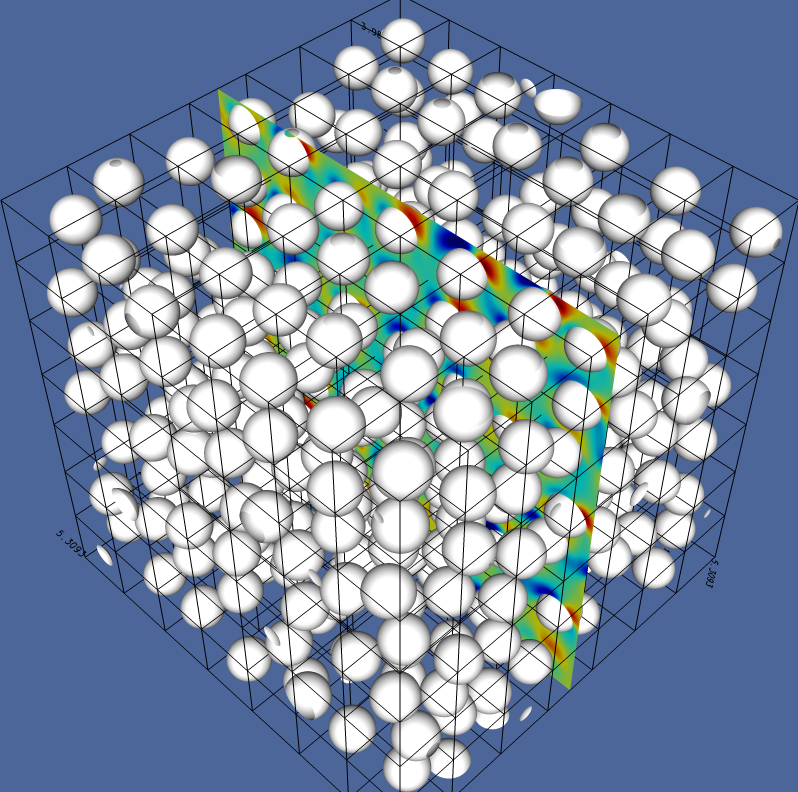
\includegraphics[width = 0.7\textwidth]{image/3D/sim49.png}}
\end{center}
%================================================================


\vfill

%================================================================

\vspace{1em}
\noindent{\large\textbf{Home structure~:} IFPEN Solaize}

\vspace{1em}
\noindent{\large\textbf{Director~:} Stephane \textsc{Popinet}
\footnote[1]{\footnotesize Sorbonne Université, \texttt{21, rue de l'école de médecine, 75006 Paris}. \url{https://www.sorbonne-universite.fr/}}
}

\vspace{1em}
\noindent{\large\textbf{IFPEN supervisors ~:} Jean-Lou \textsc{Pierson}
\footnote[2]{\footnotesize IFP Energies Nouvelles, \texttt{Rond-point de l'échangeur de Solaize, 69360 Solaize}. \url{https://www.ifpenergiesnouvelles.fr/}}
}

%================================================================

\vfill

%================================================================

\includegraphics[height=1.2cm]{image/Logo_IFPEN.png}
\hfill

\includegraphics[height=1.6cm]{image/Sorbonne.jpg}

%================================================================

\end{titlepage}
\makeatother

%================================================================


\phantomsection\addcontentsline{toc}{chapter}{Front matter}
\chapter*{\centering Abstract}
\phantomsection\addcontentsline{toc}{section}{Abstract}

Buoyancy-driven droplet flows are encountered in many chemical engineering processes such as gravity separators and liquid-liquid extractors. 
These systems exhibit a wide range of scales, from the size of individual inclusions (as small as a few micrometers) to the size of the reactor (often exceeding one meter), making fully resolved simulations computationally impractical.
As a result, the current engineering practice relies on averaged equations of motion for both the dispersed and continuous phases.

Regarding the modeling of dispersed two-phase flows, previous studies have primarily focused on suspensions of solid spherical particles. 
However, significantly less work has been devoted to the modeling of emulsions. 
Hence, the primary focus of this PhD work is the derivation of a set of averaged equations capable of describing suspensions of arbitrarily shaped fluid inclusions and complex surface properties. 
The dispersed phase is represented through Lagrangian-averaged conservation laws, while the continuous phase is modeled using Eulerian-averaged conservation laws. 
Consequently, this formalism is referred to as the ``hybrid model''. 

The second aspect of this PhD is the development of closure models to feed the equations of the ``hybrid model''. 
Specifically, we derive closure laws for the momentum and energy-averaged equations in the dilute and Stokes flow regimes considering mono-disperse emulsions of spherical droplets. 
These theoretical investigations are supplemented by Direct Numerical Simulations (DNS) of buoyant emulsions of droplets, conducted using the open-source code \texttt{Basilisk C}. 
Based on theoretical analysis, DNS results, and findings from the literature, we propose models for the interphase drag force, stresslet tensor, and Reynolds (or pseudoturbulence) stress tensor applicable to rising homogeneous emulsions with finite inertial effects and in non-dilute regimes. 
Our results suggest that including the drift velocity contribution, not only in the inter-phase drag force but also in the effective stress of the continuous phase averaged momentum equation, is essential to model the rheology of emulsions. 

The final contribution of this work concerns the study of the nearest-particle Statistics pair distribution, used to characterize the microstructure of the emulsion and the relative kinematics   of interacting droplets.
It is shown that the microstructure geometry can be described using the second moment of the nearest-particle pair distribution, which quantifies features such as clusters and layers of droplets.
We then analyze the microstructure kinematics through the derivation of a transport equation for this quantity.
In particular, it is shown that the mean interaction time of droplets corresponds to the relaxation time of the second moment of the nearest-particle pair distribution. 
Hence, this timescale governs the formation of the microstructure.


% Overall this PhD work offers mathematical tools necessary to model emulsions within a multiscale ``hybrid'' approach.


\newpage
\chapter*{\centering R\'esum\'e}
\phantomsection\addcontentsline{toc}{section}{R\'esum\'e}

 
Les \'ecoulements de gouttes entra\^in\'es par la flottabilit\'e se rencontrent dans de nombreux proc\'ed\'es de g\'enie chimique, tels que les s\'eparateurs gravitaires et les extracteurs liquide-liquide.
Ces syst\`emes pr\'esentent une large gamme d'\'echelles, allant de la taille des inclusions individuelles (aussi petites que quelques microm\`etres) \`a celle des r\'eacteurs (souvent sup\'erieure \`a un m\`etre), ce qui rend les simulations enti\`erement r\'esolues impossibles \`a r\'ealiser avec les ressources informatiques actuelles.
Par cons\'equent, les pratiques actuelles de mod\'elisation reposent sur l'utilisation des \'equations moyenn\'ees qui d\'ecrive l'\'evolution des phases dispers\'ee et continue.


Concernant la mod\'elisation des \'ecoulements diphasiques dispers\'es, les recherches se sont principalement concentr\'ees sur les suspensions de particules solides sph\'eriques, tandis que beaucoup moins de travaux ont \'et\'e consacr\'es \`a la mod\'elisation des \'emulsions.
L'objectif principal de cette th\`ese est donc la d\'erivation d'un ensemble d'\'equations moyen\-n\'ees capables de d\'ecrire des \'ecoulements dispers\'es avec des inclusions fluides. 
La phase dispers\'ee est repr\'esent\'ee par des lois de conservation lagrangiennes  moyenn\'ees, tandis que la phase continue est mod\'elis\'ee par des lois de conservation eul\'erienne moyenn\'ees.
Ce formalisme est donc appel\'e  ``mod\`ele hybride''.

Le deuxi\`eme aspect de cette th\`ese est le d\'eveloppement de mod\`eles de fermeture pour alimenter les \'equations du  ``mod\`ele hybride'' .
Plus pr\'ecis\'ement, nous d\'erivons des lois de fermeture pour les \'equations moyenn\'ees de quantit\'e de mouvement et d'\'energie cin\'etique dans les r\'egimes dilu\'e et de Stokes, en consid\'erant des \'emulsions monodisperses de gouttes sph\'eriques.
Ces \'etudes th\'eoriques sont compl\'et\'ees par des simulations num\'eriques directes (DNS) d'\'emulsions de gouttes soumises \`a la gravit\'e, r\'ealis\'ees \`a l'aide du code open source \texttt{Basilisk C}.
Avec les analyses th\'eoriques, r\'esultats DNS, et des donn\'ees de la litt\'erature, nous proposons des mod\`eles pour la force de tra\^in\'ee interphasique et le tenseur des contraintes de Reynolds (ou pseudoturbulence), applicables aux \'emulsions homog\`enes ascendantes dans des r\'egimes non dilu\'es et \`a effets inertiels finis.
Nos r\'esultats sugg\`ere que l'inclusion de la contribution de la vitesse relative entre phase dispers\'ee et continue, non seulement dans la force de tra\^in\'ee interphasique, mais aussi dans la contrainte effective de la phase continue, est essentielle pour pr\'edire la rh\'eologie des \'emulsions.

La contribution finale de ce travail concerne l'\'etude de la fonction de corr\'elation de paires des voisines les plus proches, utilis\'ees pour caract\'eriser la microstructure de l'\'emulsion et la cin\'ematique relative des gouttes en interaction.
Nous montrons que la g\'eom\'etrie de la microstructure peut \^etre d\'ecrite en utilisant le second moment de cette distribution, qui quantifie des caract\'eristiques telles que les amas et les couches de gouttes form\'es dans l'\'ecoulement.
Nous proposons ensuite d'analyser la cin\'ematique de la microstructure \`a travers la d\'erivation d'une \'equation de transport pour ce tenseur.
En particulier, il est montr\'e que le temps moyen d'interaction des gouttes correspond au temps de relaxation du second moment de la distribution des paires de particules les plus proches.
Ce temps caract\'eristique gouverne ainsi la formation de la microstructure.

\chapter*{\centering Remerciement}
\phantomsection\addcontentsline{toc}{section}{Acknowledgements}
%\begin{stretchpars}
\noindent 
Je tiens avant tout a remercier Jean-Lou Pierson de m'avoir aceuillie pour mon stage de master à l'IFPEN, puis de m'avoir acceuil une nouvelle fois pour ce sujet de thèse et enfin de m'avoir acceuil une dèrnière fois à l'IFPEN pour un post d'ingénieur ! 
Je te remerci de m'avoir fait découvrir le monde de la recherche, 
de m'avoir enseigner la ``slender-body-theory'' quand je suis arrivé, 
de m'avoir poussé toujours plus loin dans mes projet, 
et de m'avoir fait confiance dans mes idées  (car on a un peu changer le programme de la thèses),
d'être un exemple en terme de rigeurs scientique (ce qui n'était vraiment pas mon fort qd je suis arrivé), 
d'avior toujour sur répondre à mes questions et me guider dans ma thèse vers les bons papiers et livres (merci de m'avoir donné à lire "Jackson 1997" je crois que c'est avec ca que ma thèse a commencé, et de me prêter ta bible: "Jackson 2000", désolé de l'avior un peu abimé d'ailleurs !).
J'ai énormément  appris a travailler à tes cotés, un grand merci !
PS: désolé de t'avoir fait travailler les dimanches sur ma thèse,  maintenant il faut faire de la \textit{slow science} ! 

Merci à Lionel Gamet bien-sur d'avior encadré mon stage de Master 2 également, de m'avoir enseigner les subtiliées de \texttt{Linux} et (particulièrement du fameux \texttt{.rpmmacros}) et de m'avoir appris a faire des maillage butterfly.  
Un plaisir de continuer a travailler avec toi ! 
PS: merci de nous avoir aidés a organiser la soutenance de thèse car on était un peu perdu. 
 
Merci a  Stéphane popinet mon directeur de thèse pour tout ses sage conseilles qui ont su me guider durant toute ma thèse. 
Sache que c'est une fièreté pour moi d'avoir travailler avec toi et d'avoir pu contributer à ton code \texttt{Basilisk}, j'ai bceaucoup appris en matière de programmation quand je me torturais a comprendre comment était codé le \texttt{qcc.h}. 
Merci de m'avior aceuillie a la Sorbonne, et de m'avoir fait présenter mon travail à Daniel Lhuillier et Rodey Fox ce qui constitué le point de départ de ce travail.  
PS: désoloé pour toutes ces fautes d'ortographes quand tu as relu le manuscript ! 

En plus de mes enquadrant j'aimerais bien evidement remercier Daniel Lhuillier qui a pris part à la direction de cette thèse de manière  officieuse. 
Tu m'a montré qu'il était possible d'exposer et de comprendre les equations du modèle hybrid avec simplicitées et pédagogie, ce qui a donner lieu a la rédaction des 3 premier chapitres de ce manuscript, et pour ca je te remercie. 

Je tiens a remercier également les deux rapporteur de cette thèse Duan Zong Zang et Olivier Simonin pour avoir lu ce manuscript en détail et avoir mis en anvant certain problèmes et point important. 
Je remerci égalemnt les autre membre du jury Fabien Candelier, Aurore Naso et Stephane Z. 
Merci a tous les autres chercheur avec qui j'ai pu interagir regulièrement ou ponctuellement cela m'a permis de réaliser ce travail  (Prabuh nott,  Thomas Pathz, Howard Stone.)


Merci à tous les menbres du département R174 pour leurs acceuil quand je suis arrivé en thèse et pour leurs second accueil a mon arrivé en CDI. 
Merci à mes cammarades de thèse Kamel et Paul pour toutes ces discutions scientique inspirantes, et les autres discutions moin scienttifique mais tout autant inspirante; et bon courage a vous pour la suite de la thèse. 

Merci à mes autres amis proche qui se reconnaisseront, et a ma famille pour tout le soutiens porté durant ces trois ans de thèse et plus généralement dans mes étude. 

Enfin merci a Camille Chavassieux qui aura su m'éloigner du travail et m'apporter un soutiens quotidien pour être heureux et équilibré dans la vie.  

\newpage


\hypersetup{linkcolor=black}
\tableofcontents\newpage %\protect\thispagestyle{title}
\listoffigures\newpage
\addcontentsline{toc}{section}{List of figure}
\listoftables
\addcontentsline{toc}{section}{List of tables}

% \section*{Labels}
\nomenclature{$_k$}{Index of the arbitrary  phase $k$}
\nomenclature{$_c$}{Index of the continuous phase $c$}
\nomenclature{$_d$}{Index of the continuous phase $d$}
\nomenclature{$_\alpha$}{Index of the particle $\alpha$}

% \section*{Physical parameters}
\nomenclature{$V_k$}{Volume of the phase $k$  [m$^3$]}
\nomenclature{$\rho_k$}{Density of the phase $k$ [kg.m$^{-3}$]}
\nomenclature{$\mu_k$}{Viscosity of the phase $k$ [kg.m$^{-1}$.s$^{-1}$]}
\nomenclature{$\sigma$}{Surface tension coefficient [N.m$^{-1}$]}
\nomenclature{$g$}{Gravity acceleration [m.s$^{-2}$]}

% \section*{Dimensionless parameters}
\nomenclature{$Ga$}{\textit{Galileo number}}
\nomenclature{$Bo$}{\textit{Bond number}}
\nomenclature{$\mu_r$}{Viscosity ratio}
\nomenclature{$\mu_r$}{Density ratio}
\nomenclature{$N_b$}{Number of droplets}
\nomenclature{$\phi$}{Volume fraction of droplets} 


\nomenclature{$\textbf{x}$}{Macroscopic position vector}
\nomenclature{$\textbf{y}$}{Microscopic position vector}
\nomenclature{$f_k$}{Arbitrary microscopic quantity}
\nomenclature{$\mathbf{\Phi}_k$}{Arbitrary non-convective term}
\nomenclature{$\textbf{S}_k$}{Arbitrary source term}
\nomenclature{$\textbf{u}_k$}{Fluid velocity vector field}
\nomenclature{$\chi_k$}{Phase indicator function}
\nomenclature{$\textbf{n}_k$}{Unit outward normal vector}
\nomenclature{$\delta_I$}{Interface indicator function}
\nomenclature{$\textbf{y}_I$}{Interface position}
\nomenclature{$\textbf{I}$}{Unity tensor}
\nomenclature{$\textbf{u}_I$}{Interfacial velocity vector field}
\nomenclature{$\textbf{J}_I$}{Arbitrary jump field}
\nomenclature{$\kappa$}{Curvature of the interface}
\nomenclature{$M_k$}{Mass transfer term}
\nomenclature{$\textbf{T}_k$}{Stress tensor}
\nomenclature{$p_k$}{Pressure field}
\nomenclature{$\textbf{f}_I$}{Surface tension force}
\nomenclature{$\textbf{b}_k$}{Body forces term}
\nomenclature{$E_k$}{Total energy}
\nomenclature{$e_k$}{Internal energy}
\nomenclature{$\textbf{q}_k$}{Energy heat flux}
\nomenclature{$T_k$}{Temperature}
\nomenclature{$D_k$}{Thermal conductivity}
\nomenclature{$D_k$}{Thermal conductivity}
\nomenclature{$a_I$}{Area density}
\nomenclature{$\phi_k$}{Volume fraction of phase $k$}



\nomenclature{$q_\alpha$}{Arbitrary Lagrangian quantity of the particle $\alpha$}
\nomenclature{$\textbf{Q}_\alpha$}{Arbitrary dipole quantity of the particle $\alpha$}
\nomenclature{$\textbf{Q}_\alpha^n$}{Arbitrary dipole quantity of order $n$}
\nomenclature{$n$}{Number density of particles}
\nomenclature{$A_\alpha$}{Surface of the particle $\alpha$}
\nomenclature{$V_\alpha$}{Volume of the particle $\alpha$}
\nomenclature{$m_\alpha$}{Mass of the particle $\alpha$}
\nomenclature{$\textbf{p}_\alpha$}{Momentum of the particle $\alpha$}
\nomenclature{$\textbf{u}_\alpha$}{Velocity of the particle $\alpha$}
\nomenclature{$\textbf{y}_\alpha$}{Position of the particle $\alpha$}
\nomenclature{$\textbf{w}_k$}{Internal relative velocity of the particle $\alpha$}
\nomenclature{$\textbf{r}$}{Relative position vector}
\nomenclature{$E_\alpha$}{Total energy of the particle $\alpha$}
\nomenclature{$E^\sigma_\alpha$}{Surface energy of the particle $\alpha$}
\nomenclature{$\mathcal{G}_\alpha$}{Inertia tensor}
\nomenclature{$\mathcal{P}_\alpha$}{Moment of momentum tensor}
\nomenclature{$\mathcal{A}_\alpha$}{Angular momentum tensor}
\nomenclature{$\mathcal{S}_\alpha$}{Strain of momentum tensor}

\nomenclature{$\mathscr{C}_N$}{Configuration vector of $N$ particles}
\nomenclature{$P_N$}{Probability density function of $\mathscr{C}_N$ }
\nomenclature{$\Psi$}{Source term related to collision, coalesce and break-up}
\nomenclature{$\theta_\gamma$}{$\gamma^{th}$ Moments of the distribution of $P$}

\nomenclature{$\delta_\alpha$}{Particle indicator function}


% \section*{Mathematical operators}
\nomenclature{$\ddt$}{Time derivative}
\nomenclature{$\pddt$}{Partial time derivative}
% \nomenclature{$\grad$}{Local gradient operator}
\nomenclature{$\gradI$}{Local interfacial gradient operator}
% \nomenclature{$\grad$}{Global gradient operator}
% \nomenclature{$\grad\cdot$}{Local divergence operator}
% \nomenclature{$\grad_I\cdot$}{Local interfacial divergence operator}
% \nomenclature{$\grad_\mathscr{C}\cdot$}{Divergence operator of the phase space}
% \nomenclature{$\grad\cdot$}{Global divergence operator}
\nomenclature{$\avg{\ldots}$}{Ensemble or volume average operator}
\nomenclature{$\kavg{\ldots}$}{Phase average operator}
\nomenclature{$\pnavg{\ldots}$}{Particular average operator}
\nomenclature{$\Iavg{\ldots}$}{Interfacial average operator}
\nomenclature{$\gavg{\ldots}$}{Moment weighted average operator}
\nomenclature{$\mavg{\ldots}$}{Mass weighted average operator}
\nomenclature{$(\ldots)^S$}{Return the symmetric part of the argument}
\nomenclature{$(\ldots)^A$}{Return the antisymmetric part of the argument}
\nomenclature{$\Exp{\ldots}$}{Return the dipole expansion of the argument}

\printnomenclature
\addcontentsline{toc}{section}{Nomenclature}

\newpage

\printacronyms[name=List of acronym]
\addcontentsline{toc}{section}{List of acronym}
\ac{CFD}
\ac{CFD}


\mainmatter

\part{Introduction}

% \chapter{Introduction}
\label{part:intro}

\tb{Clearly more on floation etc... ask for picture }
\section{Industrial challenges} 
Sedimentation of particles falling or rising under the action of gravity through a fluid is frequently used in a variety of industrial and natural processes, such as food processing, cosmetics, petroleum production, and environmental remediation. 
It is an efficient way to separate solid particles or droplets from the surrounded fluid. 
The clarification of waste water makes use of such a physics, the particles or droplets rise up due to buoyancy forces, afterward they are ejected from the mixture.
Even through numerous experimental and theoretical studies have been conducted on this topic, models are still very restricted and show a significant lack of accuracy. 
In the Perspective of reducing the cost and the environmental impacts of energy processes involving multiphase flows, IFP Energies Nouvelles and public funds, supply finance for the theoretical as well as for experimental research on multiphase flows.
Therefore, this thesis focus on the theoretical and numerical modeling of buoyant emulsion in the context of water waste treatment.  


\section{A multiscale problem} 
The Liquid /Liquid multiphase flows often involve multiscale physical phenomenons. 
Indeed, at the scale of the vessel we can consider the mixture as a homogeneous phase.
The physical properties and the hydrodynamics of the mixture, will depend on the microscale properties and the phases' interactions.
In the context of droplets those interactions are of two kinds. 
The first one is the hydrodynamical interactions between the dispersed phase and continuous phase.
Here, the scale of interest is the droplet scale.
The second type of interaction come from the van der Walls forces which act at the molecular scale. 
Then, we can already identify $3$ scales in this problem.
The scale of the bulk, or the vessel, where the medium seems homogeneous. 
The scale of the droplets, where hydrodynamic forces drive the flow. 
And finally, the molecular scale or the interface scale, where the chemical interaction drive the motions. 
Note that the chemical interactions also involve surfactant which won't be treated in this thesis. 

The link between the vessel's scale and the droplets' scale is usually made using averaged technics. 
It consists in averaging the constitutive equations, that drives the physics at the drop scale, to the reactor scale. 
For isothermal Newtonian flow we generally use the averaged Navier-Stokes equations \citep{jackson1997locally}. 
When we consider specific types of particles or fluid, we need to apply some changes to these equations. 
These averaged equations regardless of the hypothesis taken, involve what we call closure terms.
Those closures are the mathematical expression of the nature of the microstructure.
As an example the averaged drag force on the particles, the velocity fluctuations and the averaged torque and higher moments are closures terms. 
To solve those equations one needs a precise expression of the closure terms. 
Another problem tackled by averaged equations is the modeling of the local size distribution of the droplets. 
The distribution of size can be affected through migration of particles that have different rising velocity as a consequence of their size, and through coalescence and break up of the droplets. 
Note that the particle size distribution is of a major importance as the drag force and the other closure terms depends on it. 
Then, the most challenging part of this problem is not to solve the averaged equations, but rather to find empirical or theoretical closures. 
Regarding the link between the molecular scale and the upper scales, it is done through the modeling of chemical interactions.
Indeed, while the droplets are in contact chemical interaction influence greatly the probability of coalescence and therefore the coalesce rate. 
As a consequence it changes the drops size distribution too.

\section{Non-exhaustive authors cartography of particles suspension dynamics} 
\begin{figure}[h!]
    \begin{tikzpicture}[thick, scale=1, every node/.style={scale=0.5}]
        \node (img) at (0,0){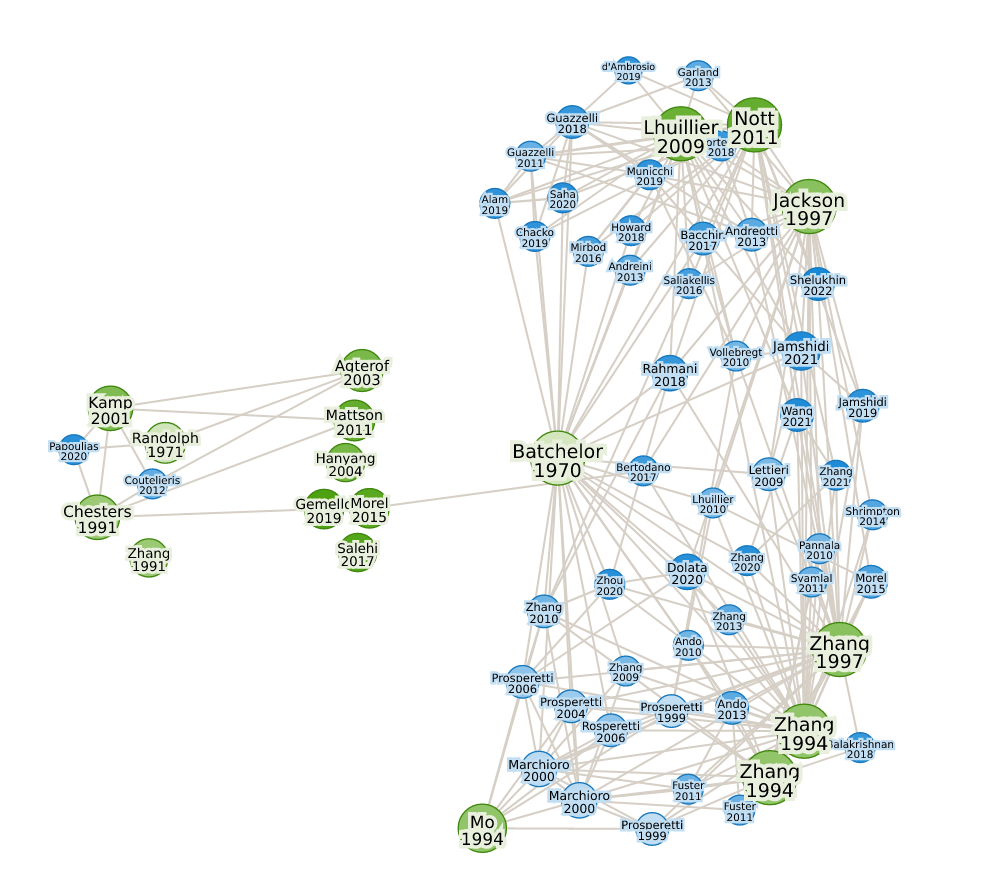
\includegraphics[width=2\textwidth]{Bib/graph70_paperGraph_network.png}};
        \draw[dashed,very thick](-2,-0.5)ellipse(1 and 2.5);
        \draw[dashed,very thick](-5,-0.5)ellipse(1.5 and 2.5);
        \draw[dashed,very thick](4,4)ellipse(2 and 1.5);
        \draw[dashed,very thick](4.5,-4)ellipse(1.5 and 2);
        \draw[dashed,very thick](4,5)node[above,very thick]{\Large$\bm{(III)}$};
        \draw[dashed,very thick](6,-5)node[right,very thick]{\Large$\bm{(II)}$};
        \draw[dashed,very thick](-6.5,2)node[above,very thick]{\Large$\bm{(I)}$};
        \draw[dashed,very thick](-1.3,1.75)node[above,very thick]{\Large$\bm{(IV)}$};
        % \draw[<->](com2.north)--(com3.south)node[midway]{Equivalent};
    \end{tikzpicture}
    \caption{Non-exhaustive cartography of the different publications on population balance models and averaged equations. The articles are represented by the name of the first author. The lines between each article mean that both articles cited each other.}
    \label{fig:carte}
\end{figure}
\ref{fig:carte} summarize the main area related to the theoretical modeling of emulsion through the averaged technics. 
The $\bm{(I)}$ field correspond to the modeling of coalescence and break up phenomenon in a drop or bubbles suspension.
It includes the Population Balance Model (PBM) theory.  
But also the modeling of the film drainage when two drops nearly coalesce. 
Indeed, \citet{randolph2012theory} introduced the first population balance models, at the origin it was designed  for Crystallizes. 
Then, \citet{chesters1991modelling} studied the hydrodynamical and chemical interaction of a pair of droplets leading to coalesce.
And finally, we can observe the first model of PBM including coalescence for a population of droplets \citep{KAMP20011363}.  
The $\bm{(II)}$ and $\bm{(III)}$ area are the authors who studied the averaged equations.
Most of them considered mono-dispersed suspension, therefore the PBE is not involved.
Rather they focused on closing the averaged equations theoretically. 
We consider two district formalism, the one represented here by the main article, \citet{jackson1997locally} and the other by \citet{zhang1994averaged}.
The first one makes use of volume average method and the second one of ensemble average method (those methods will be discussed in \ref{chap:avg}).
To model a poly-disperse suspension of particles (either solid, bubbles or droplet) one has to links the two former theories together, \citep{morel2015mathematical}. 
However, the current state of the art regarding droplets suspension is incomplete.
Therefore, in \ref{chap:avg}, after an entire review of the bibliography, we carry out the derivation of a generalized hybrid model for droplets particles. 
We will see that each of the terms of the averaged equations have a well-defined physical sense related to the nature of the particular phase. 
Then, we address the problematic of the identification of the essential closure terms, and evaluate their relative error while neglecting specific terms. 
Then, in \ref{chap:DNS} we tackle the problematic of the finding of closure terms through Direct Numerical Simulation (DNS).
After identifying the related investigation in the literature, we present our own model and a glimpse of our results in \ref{chap:mono-disperse}. 

\tb{introduce the main equations}

\part{Statistical modeling of dispersed two phase flows}

%%%%%%%%%%%%%%%%%%%%%%%%%   CHAPITRE 1
\chapter{The hybrid model for arbitrary fluid particles}
\localtableofcontents


\section{Introduction}

%Dispersed multiphase flows are ubiquitous in chemical engineering processes. 
%Examples include gas-solid flows in fluidized bed reactors, liquid-liquid flows in liquid-liquid extractors, and bubbly flows in flotation processes. 
%Developing a versatile model capable of capturing the various nature of the dispersed multiphase flow is therefore essential.
%In this work we aim to bridge the existing gaps in current models by providing a unified and adaptable framework for any kind of dispersed multiphase flow problems including interfaccial transport equation.

Dispersed multiphase flows are encountered across a wide range of chemical engineering applications. 
These include gas-solid interactions in fluidized bed reactors , liquid-liquid flows in extractors, and gas-liquid bubbly flows in flotation processes. 
These systems exhibit a wide range of scales, from the size of individual inclusions (as small as a few micrometers) to the size of the reactor (often exceeding one meter), making fully resolved simulations computationally impractical. 
As a result, the current engineering practice relies on averaged equations of motion for both the dispersed and continuous phases. 
Therefore, developing a robust set of averaged equations that accurately captures the complexities of dispersed multiphase flows is essential. 
In this study, we aim to overcome the limitations of existing models by proposing a comprehensive set of averaged equations that can be applied to various types of dispersed multiphase flows, including interfacial transport processes.

%Due to the two many scales encountered in this process ranging from the particle size (from let'say 10 micrometer) to the reactor size (larger thant one meter) it appears to be unfeasible to model the process into play using fully resolved simulations.
%The current engineering practice is to relay on averaged set of equation of motion for both the dipsersed and continuous phase equation.
%Therefore, it is essential to develop a rigorous set of averaged equations that can accurately represent the diverse behaviors of dispersed multiphase flows. 
%In this study, our goal is to address the limitations of existing models by proposing a comprehensive averaged set of equations that can be applied to various kind of dispersed multiphase flow, including interfacial transport equations. %framework 

%Most of the averaged two-fluid models relies on the framework proposed by \citep{drew1983mathematical} where both dispersed and continuous phase are treated in a similar fashion (see \citet{hu2021cfd} for instance).
%Despite its very versatility (this framarwork may be used for non dispersed flows such as stratified or slug flow), the phisical meaning of the closure terms are difficult to obtain \citep{drew1983mathematical} and the mathematical well posdeness of the whole system is sill a matter of debate \citep{panicker2018hyperbolicity,lhuillier2013}.
%Another treatment of the dispersed phase is possible and by treating properly the dispersed phase in a lagrangian framework.
%This framework takes it root from the kinetic theory of gases in which the motion of the particles is described by the single-particle distribution function which obeys Botlzmann equation \citep{chapman1990mathematical}. 
%This approach have been very succesfull in predicting the motion of dry granlaur material \citep{rao2008introduction} or gas-solid flows \citep{simonin1996}.
%The main problematic of this framework is that the fluid phase and the dispersed phase are treated using two disting formalism: phase averaged for the fluid phase and lagrangian averaging for the particle average.
%In a pioneering study \citet{buyevich1979flow} demonstrated that both averaging formalism can be linked, by performing a Taylor expansion of the closure terms around the center of mass of the particle.
%Then, this framework was revisited by \citet{lhuillier1992} and \citet{zhang1994averaged,zhang1994ensemble}. 
%The latter provided closures in the inviscid flow limit for the mass and momentum transport equation.
%Numerous example of averaged dispersed two-phase flows model have been proposed this last two decades.
%After that \citet{jackson1997locally,zhang1997momentum} derive the averaged conservation equations for a solid spherical particle suspension.
%They provided the closure in the stokes flow limits.  
%As started by \citep{zhang1994averaged,zhang1994ensemble} where they study spherical bubbles suspension.
 
The majority of averaged two-fluid models are based on the framework proposed by \citet{drew1983mathematical}, where both the dispersed and continuous phases are treated similarly (see, for example, \citet{hu2021cfd}). 
Despite its versatility-allowing applications beyond dispersed flows, such as stratified or slug flow-the physical interpretation of the closure terms remains difficult \citep{drew1983mathematical}, and the mathematical well-posedness of the entire system is still a matter of debate \citep{panicker2018hyperbolicity, lhuillier2013}.
An alternative approach treats the dispersed phase using a Lagrangian framework. 
This approach originates from kinetic theory of gases, where the motion of particles is described by a single-particle distribution function governed by the Boltzmann equation \citep{chapman1990mathematical}. 
It has proven particularly successful in predicting the dynamics of dry granular materials \citep{rao2008introduction} and gas-solid flows \citep{simonin1996}. 
However, the fluid phase and the dispersed phase are handled through two distinct formalisms: phase averaging for the fluid and Lagrangian averaging for the dispersed phase.
In a pioneering study, \citet{buyevich1979flow} demonstrated that these two averaging methods could be connected by performing a Taylor expansion of the closure terms around the particle’s center of mass. 
This "hybrid" formalism was later revisited by \citet{lhuillier1992ensemble}, and by \citet{zhang1994averaged, zhang1994ensemble}. The latter provided closures for the momentum transport equations in the inviscid flow limit. 
Subsequently, \citet{jackson1997locally} derived averaged conservation equations for a suspension of spherical solid particles, providing closures for the Stokes flow regime.

%Most of the previous authors working on the "hybrid" formalism considered solid particles \citet{buyevich1979flow,jackson1997locally}. 
%A notable exception is the work of \citet{zhang1994ensemble} who considered spherical bubble with time dependent radii and \citet{zhang1997momentum} who considered spherical drops.  %They all derived Lagrangian based equations for the dispersed phase considering point of mass spherical particles.
%But then how to account for different inclusion shapes, fluid internal motion and transport equations on the surface within these Lagrangian models ?
%Indeed, to the best of our knowledge, the surface properties such as surface tension and chemical concentration of surfactant over the surface, have not been taken into account into such averaged hybrid model. 
%While it is of major importance to predict the hydrodynamics bubbly flows.
%Although the lagrangian form of surface transport equations is well known \citet{lhuillier2000bilan} is application to define a general lagrangian quantities remains unknown.
%Therefore, a whole in one, hybrid model that encapsulate all the physics, meaning, surface properties, particles of arbitrary shape, higher moments equations is needed. 

Many previous studies that used the "hybrid" formalism have focused on solid particles \citep{buyevich1979flow,jackson1997locally}. 
Notable exceptions include \citet{zhang1994ensemble}, who investigated spherical bubbles with time-varying radii, and \citet{zhang1997momentum}, who examined spherical droplets. 
Despite these advancements, the question remains: how can different inclusion shapes, internal fluid motion, and surface transport equations be incorporated into such Lagrangian models? 
To the best of our knowledge, important surface properties-such as surface tension and the distribution of surfactants-have yet to be integrated into these averaged hybrid models. 
While the Lagrangian formulation of interfacial area equation is well established \citep{lhuillier2000bilan}, its application to define general Lagrangian quantities for a dispersed phase is still not fully explored. 
Thus, there is a need for a comprehensive hybrid model that encompasses all relevant physical aspects, including surface properties, arbitrarily shaped particles.%, and higher-order moment equations.


%Even though these hybrid models for fluid particles were already quite sophisticated it still misses some major points. 

% Additionally, a proper and general derivation of these models must be established in the most general case possible, i.e. for any kind particles and conservation laws. 



%Some author tried to model fluid particle within a Lagrangian approach and already answered part of these questions.  
%Among them \citet{lhuillier2000bilan} and \citet{morel2015mathematical,zaepffel2012multisize} applied the Lagrangian framework equations for fluid particle with mass transfer. 
%These model consist in establishing the conservation equation of an integrated Eulerian quantity $f$, within the volume of a particle denoted by $\Omega_\alpha$, namely  $\int_{\Omega_\alpha} f d\Omega$. 
% Likewise, the so-called first moments of a quantity $f$ is defined by $\int_{\Omega_\alpha} \textbf{r} f_k d\Omega$ with \textbf{r} the position from the center of mass to any point in the volume of the particle. 
% These integrals can be derived within time and yield the moments conservation equitation for any Lagrangian moment, , of the particle $\alpha$. 

Several authors have addressed the question of equivalence between Lagrangian (or particle-averaged) and phase-averaged equations in various contexts \citep{zhang1997momentum,lhuillier2000bilan,nott2011suspension}. 
In \citet[Appendix A]{zhang1997momentum}, the authors demonstrated that these two frameworks are equivalent for spherical inclusions when only considering the firt order moments. 
Later, \citet[Appendix A]{nott2011suspension} extended the proof of \citet{zhang1997momentum}, showing that the Lagrangian and phase-averaged equations are strictly equivalent for suspensions of solid spherical particles by considering an infinite number of higher-order terms. 
In addition, \citet{lhuillier2010multiphase} argued that the phase-averaged equations applied to the dispersed phase are, in fact, a Taylor series expansion of the particle-averaged moment equations.
Similarly, in the context of interfacial area balance equations, \citet{lhuillier2000bilan} reached a comparable conclusion when comparing the phase-averaged and particle-averaged area density equations for spherical particles. 
These studies focus on monodisperse suspensions of spherical particles and all arrive at the same conclusion: the particle-averaged equation is rigorously equivalent to the phase-averaged equation for the dispersed phase.
In this work, we extend these results by providing a general proof of the equivalence between the phase-averaged and particle-averaged frameworks for inclusions of arbitrary shapes, including interfacial transport effects.




%Another question that has been addressed by several authors \citep{zhang1997momentum,lhuillier2000bilan,nott2011suspension} is the one of the equivalence between Lagrangian or particle-averaged and phase-averaged equations. 
%In \citet[Appendix A]{zhang1997momentum} they provided a demonstration that both formalism are equivalent at first order of tthe Taylor expansion for spherical inclusions.%for the momentum equation of tspherical . 
%In a different context of nterfacial area balance equation \cite{lhuillier2000bilan}  reached a similar conclusion when comparing the phase-averaged area density and particle-averaged area density equations for spherical particles. 
%Next, \citet[Appendix A]{nott2011suspension} provided the proof that  Lagrangian or particle-averaged and phase-averaged equations were strictly equivalent for suspension of solid spherical particles even considering an infinite number of higher order terms. 
%In \citet{lhuillier2010multiphase} they state that the phase-averaged equation applied on the dispersed phase is in fact a Taylor series expansion of the particular-averaged moments equations. 
%In all these studies they focus  mono-disperse spherical particle suspension and all reached the same conclusion, i.e. the particular-averaged linear momentum equation is rigorously equivalent to the phase-averaged momentum equation for the dispersed phase. 
%Here, we provide a general proof of the equivalence between phase-averaged framework and particle-averaged framework for an arbitrary shaped inclusion with interfacal tarnsport. 
%\citet[Appendix A]{zhang1997momentum} provided evidences that the particle-averaged momentum equation is as legitimate as the phase-averaged momentum equation, which is consistent with \ref{eq:proof2}. 
%Additionally, \citet[Appendix A]{nott2011suspension} derived a similar expression than \ref{eq:proof2}, also in the case of the averaged momentum equation for suspension of solid spherical particles.
%This demonstration has been derived for the area density concentration of spherical particles. 
%however, they reach a compatible but different conclusion. 

% Finally, to gives a more specific insight of the use of such a model in the practical cases, we take the example the contaminated rising bubbly flow. 
% In particular, we demonstrate how to derive a model to predict the distribution of surfactant over the interface of bubbles, as it is of major importance to predict mass transfer and drag force correlation \citep{kentheswaran2022direct}.
% Additionally, we also show how to derive the orientation tensor equation in fibrous media. 

%In this article we derive the a general hybrid model for disperse two phase flow with interfacial transport. 
%We start in \ref{sec:two-fluid} to expose the two-fluid formulation and the distributional form of the interfcaial transport equation. 
%Then, in \ref{sec:Lagrangian} we propose a Lagrangian-based model to describe each inclusion fluid particles with arbitrary shapes and surface properties.
%In \ref{sec:averaged_eq} we provide a demonstration that the particle-averaged equation is rigorously equivalent to the phase-averaged equation for any kind of dispersed multiphase flow and conservation law. 
%From this demonstration we present the hybrid set of conservation equations consisting of one equation for the fluid phase and an arbitrary number of equations for the dispersed phase repereseting the conservation of moments.
%The findings obtained in the course of the investigation are discussed in \ref{sec:conclusion}.
In \ref{sec:two-fluid}, we begin by presenting the two-fluid formulation and the distributional form of the interfacial transport equation. 
Next, in \ref{sec:Lagrangian}, we introduce a Lagrangian-based model that describes individual fluid particles with arbitrary shapes and surface properties. 
In \ref{sec:averaged_eq}, we demonstrate that the particle-averaged equation is rigorously equivalent to the phase-averaged equation for any type of dispersed inclusions. 
Building on this demonstration, we introduce a hybrid set of conservation equations, consisting of one equation for the fluid phase and multiple equations for the dispersed phase, representing the conservation of moments. 
Finally, we discuss the findings of this investigation in \ref{sec:conclusion}.
%based on the local conservation laws presented 
%Then we present the Lagrangian balance on an arbitrary particle.  
%conclude that the particle-averaged equations are sufficient to describe every aspect of the flow since they compose the phase-averaged equation.%, which confirm the affirmation of \citet[Appendix A]{zhang1997momentum}. 
%With the use of this general framework we are now able to identify in which circumstance the specific properties of the particles such as, internal velocities, shape, and surface tension forces, come into play in the averaged model. 
%The organization of this manuscript is as follows. 
%It is then demonstrated how to perform an average onto these equations to obtain the classical two-fluid formulation of two phase flows. 
%By deriving these time varying integrated properties along with applying an averaging procedure on these equations, we are able to derive a Lagrangian model for fluid particles. 

\JL{TO DO.
\begin{itemize}
    \item faire une derniere passe en faisant attention aux notations (par exemple $\text q_\alpha$ qui ne doit pas etre en italique), à l'anglais, aux coquilles de tout type
    \item je n'ai pas relu ni l'annexe C ni l'annexe D. Mais dans ces dernieres il faudrait specifier ce que veut dire le signe $[]$ ou le remplacer par une notation plus usuelle.
\end{itemize}

}




\section{The two-fluid formulation}
\label{sec:two-fluid}

\label{sec:two-fluid}

We consider a system made of two phases, $\Omega_1(t)$ and $\Omega_2(t)$, separated by a sharp interface $\Sigma$(t), that fill the considered domain $\Omega \subset \mathbb{R}^3$, in such a way that $\Omega = \Sigma(t) \cup \Omega_1(t) \cup \Omega_2(t)$ (see \ref{fig:Scheme}). 
These domains obey the same mathematical constrains as defined in \cite{bothe2022sharp}. 
To track the position of the phases we define the Phase Indicator Function (PIF), 
\begin{equation}
    \chi_k(\textbf{y},t) =  \left\{
      \begin{tabular}{cc}
        $1 \;\text{if} \;\textbf{y} \in \Omega_k(t)$\\
        $0 \;\text{if} \;\textbf{y} \notin \Omega_k(t)$
      \end{tabular}
      \right.
      \text{for $k \in 1,2$}
      \label{eq:PIF}
\end{equation}
\begin{figure}[h!]
    \centering
    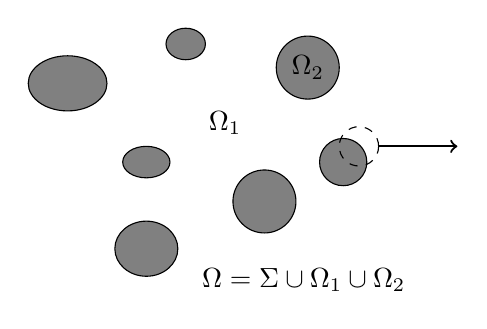
\begin{tikzpicture}
        \foreach \x/\y/\ra/\r in {
        1/3/0.2/0.25,
        2.55/2.7/0.4/0.4,
        0.5/0.4/0.35/0.4,
        2/1/0.4/0.4,
        3/1.5/0.3/0.3,
        0.5/1.5/0.2/0.3,
        -0.5/2.5/0.35/0.5}{
            \draw[fill=gray](\x,\y) ellipse(\r cm and \ra cm);
        }
        \draw[dashed](3.2,1.7)circle(0.25);
        % \draw[thick,->](3.2,1.7)++(0.1767,0.1767)--++(0.4,0.4)--++(1,0);
        \draw[thick,->](3.2,1.7)++(0.25,0)--++(1,0);
        \draw(2.55,2.7)node{$\Omega_2$};
        \draw(1.5,2)node{$\Omega_1$};
        \draw(2.5,0)node{$\Omega = \Sigma \cup \Omega_1 \cup \Omega_2$};
        % \draw(2.5,-1)node{$\Sigma = \sum_\alpha \Sigma_\alpha$};
        % \draw(2.5,-0.5)node{$\Omega_2 = \sum_\alpha \Omega_\alpha$};
    \end{tikzpicture}
    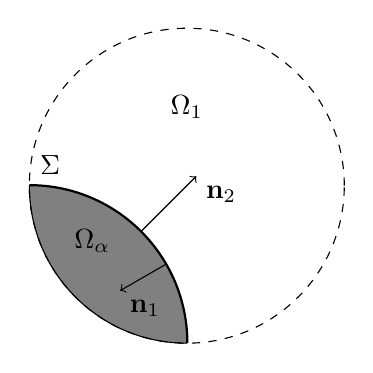
\begin{tikzpicture}%[scale = 0.9]
        \draw[very thick](0:2)arc(0:90:2)node[above right]{$\Sigma$};
        \draw[fill=gray](0:2)arc(0:90:2)arc(180:270:2);
        \draw[dashed](2,2)circle(2);
        \draw[->](1.42,1.42)--++(0.7,0.7)node[below right]{$\textbf{n}_2$};
        \draw[->](1.73,1)--++(-0.577,-0.333)node[below right]{$\textbf{n}_1$};
        \draw(2,3)node{$\Omega_1$};
        \draw(0.8,1.3)node{$\Omega_\alpha$};
    \end{tikzpicture}
    \caption{Scheme of the topology of dispersed two phase flows.}
    \label{fig:Scheme}
\end{figure}
From now on the $k$ indies will refer to either the phase $1$ or $2$, and we drop the time and position arguments in each functions. 
Then, the transport equation of $\chi_k$ can be written as \citep{drew1983mathematical,kataoka1986local,morel2015mathematical},
\begin{equation}
    \pddt \chi_k
    + \textbf{u}_I \cdot \nablabh \chi_k
    = 0,
    \label{eq:dt_chi_k}
\end{equation}
where $\textbf{u}_I$ is the velocity of $\Sigma(t)$.
Besides, it can be shown \citep{tryggvason2011direct,drew1983mathematical,kataoka1986local,bothe2022sharp} that,
\begin{equation}
    \nablabh \chi_k
    = - \delta_I \textbf{n}_k
    \label{eq:grad_chi_k}
\end{equation}
where we have introduced the Interface Indicator Function (IIF) defined as $\delta(\textbf{y}-\textbf{y}_I)$, with $\delta$ being the Dirac-delta function and $\textbf{y}_I$ the position vectors lying on the domain $\Sigma(t)$.
We also define $\textbf{n}_k$ as the outward normal vector of the domain $\Omega_k$.
Taking the gradient of \ref{eq:dt_chi_k} yields the IIF transport equation namely,
\begin{equation}
    \pddt \delta_I
    + \nablabh \cdot \left[(\textbf{u}_I\cdot\textbf{n})\textbf{n} \delta_I\right]
    = \delta_I (\textbf{u}_I\cdot\textbf{n})(\nablabh \cdot\textbf{n})
\end{equation}
As pointed out by \citet{morel2007surface}, it is more convenient to rewrite this equation under the following form,
\begin{equation}
    \pddt \delta_I
    + \nablabh \cdot (\delta_I \textbf{u}_I)
    = \delta_I \nablabhI \cdot \textbf{u}_I.
    \label{eq:dt_delta_I}
\end{equation}
where we introduced the surface divergence operator defined as $\nablabhI \cdot ()= (\textbf{I}-\textbf{nn})\cdot \nablabh \cdot ()$.
Likewise, we can derive an expression for the gradient of $\delta_I$ by taking the gradient of \ref{eq:grad_delta_I} yielding,
\begin{equation}
    % &
    \nablabh\delta_I 
    = \textbf{n} \cdot \nablabh (\textbf{n} \delta_I),
    % &
    % \pddt\delta_I 
    % = - \textbf{n} \cdot \nablabh (\textbf{u}_I  \cdot \textbf{n} \delta_I)
    \label{eq:grad_delta_I}
\end{equation}


Let $f_k(\textbf{y})$ being a volumetric property of the flow solely defined in $\Omega_k(t)$.
Likewise, let $f_I(\textbf{y})$ be an arbitrary surface property defined on $\Sigma(t)$.
Then it is possible to derive the local conservation equations for volumetric and surface quantities \citep{bothe2022sharp,morel2015mathematical,tignol1986modelisation}, using Reynolds transport theorem  and divergence theorem on an arbitrary control volume.
These conservation laws read as, 
\begin{align}
    \label{eq:dt_f_k}
    \pddt f_k
    &= \nablabh \cdot \left(
        \bm{\Phi}_k
        - f_k\textbf{u}_k
        \right)
    + \textbf{S}_k
    & \text{ in } \Omega_k,&\\
    \pddt f_I  
    &= 
    \nablabhI \cdot (\mathbf{\Phi}_{I||} - f_I \textbf{u}_I)
    + \textbf{S}_I
    - \Jump{
        f_k (\textbf{u}_I - \textbf{u}_k)
        + \mathbf{\Phi}_k
     } 
    & \text{ on } \Sigma&
    \label{eq:dt_f_I}
\end{align}
for respectively the volumetric and surface properties.
In \ref{eq:dt_f_I} we introduced the notation $\Jump{\ldots}$ to indicate the sum over both phases, i.e. $\sum_{k=1}^2 [\ldots] \cdot \textbf{n}_k$. 
Where we introduced $\bm{\Phi}_k$ and $\bm{\Phi}_I$ as the non-conservative flux tensor corresponding to $f_k$ and $f_I$. 
The non-conservative flux is often expressed through a constitutive equation depending on the nature of the flow such as the stress tensor for the momentum.
$\textbf{S}_k$ and $\textbf{S}_I$ is defined as the volumetric source term of respectively the phase $k$ and at the interface $\Sigma$.
It is important to notice that \ref{eq:dt_f_k} and \ref{eq:dt_f_I} are solely defined in respectively $\Omega_k$ and $\Sigma$, therefore these equations are referred as local conservation equations.

To generalize these equations over the domain $\Omega$ we follow the formalism of \citet{drew1983mathematical,marle1982macroscopic} and \citet{kataoka1986local} for the volumetric quantities.
Indeed, to any local quantities $f_k$ defined in $\Omega_k$, we assign the field $\chi_k f_k$ which is defined in $\Omega$. 
Similarly, for any local surface quantities $f_I$ defined on $\Sigma$ we assign the field quantity $\delta_I f_I$ defined on $\Omega$. 
Then, multiplying \ref{eq:dt_f_k} and \ref{eq:dt_f_I} by respectively $\chi_k$ and $\delta_I$, and making use of \ref{eq:dt_chi_k} and \ref{eq:dt_delta_I} gives, 
\begin{align}
    \pddt (\chi_k f_k)
    &= \nablabh \cdot (\chi_k \bm{\Phi}_k - \chi_k f_k \textbf{u}_k)
    + \chi_k \textbf{S}_k
    + \delta_I\left[
        \bm{\Phi}_k
        + f_k
        \left(
            \textbf{u}_I
            - \textbf{u}_k
        \right)
    \right]
    \cdot \textbf{n}_k ,
    % & \forall \textbf{y} \in \Omega&
    \label{eq:dt_chi_k_f_k}\\
    \pddt (\delta_If_I)  
    &= 
    \nablabh \cdot (\delta_I \mathbf{\Phi}_{I||} - \delta_I f_I \textbf{u}_I)
    +\delta_I\textbf{S}_I 
    - \delta_I \Jump{
    f_k (\textbf{u}_I - \textbf{u}_k)
    + \mathbf{\Phi}_k
    }.
    \label{eq:dt_delta_I_f_I}
\end{align}
We obtained $k$'s equations defined over the domain $\Omega$ for the bulk quantities, and third global equations for the surface quantities also valid over $\Omega$. 
The transformation of these equations from local to global conservation makes appear a term on the RHS of \ref{eq:dt_chi_k_f_k} representing the interfacial transfer of $f_k$ and $\mathbf{\Phi}_k$, while the surface transport equation did not change fundamentally. 
The set of equations formed by \ref{eq:dt_chi_k_f_k} for $k =1,2$ is commonly known as the \textit{two-fluid} formulation of multiphase flows, to which we add the \textit{jump condition} across the phase given by \ref{eq:dt_delta_I_f_I} \citep{morel2015mathematical,tryggvason2011direct,drew1983mathematical,kataoka1986local}. 
In this work, we prefer to think of those equations as a set of three equations, formed by \ref{eq:dt_chi_k_f_k} for the volumetric conservation equations and \ref{eq:dt_delta_I_f_I} for the surface conservation equations. 

Now that we properly defined the volumetric and surface conservation laws over $\Omega$, let's derive of two phase flows.
We now define any bulk quantity $f$ as $f = \sum_k \chi_k f_k + \delta_I f_I$.
Then adding \ref{eq:dt_chi_k_f_k} for $k=1,2$ and \ref{eq:dt_delta_I_f_I} give the commonly known as the \textit{single-fluid} formulation,
\begin{equation}
    \pddt f
    = \nablabh \cdot (\bm{\Phi} - f \textbf{u})
    + \textbf{S}.
    \label{eq:dt_f}
\end{equation}
Actually, it is more common in the literature to define the bulk quantities as $f = \sum_k \chi_k f_k$ and consider the interfacial terms as source terms as it is often neglected \citep{morel2015mathematical,tryggvason2011direct}. 
Nevertheless, in this work we consider a general case without approximation therefore it is more convenient to think of the bulk quantities as a sum of three phase quantities. 

\subsection{The averaged conservation equations}
\label{sec:avg_def}
In this study, we employ the ensemble average technique to establish the averaged conservation equations. 
This method is just one of several averaging approaches, including the volume average method \citep{jackson1997locally} and time averaging \citep{ishii2010thermo}. 
Despite their differences, all these techniques yield the same set of averaged equations \citep{jackson1997locally,zhang1997momentum}.
In the following we recall some properties of the ensemble average operator. 
Let, $P(\FF)$ be the probability density function that describes the probability of finding the flow in the configuration $\FF$. 
We note $d\PP = P(\FF) d\FF$ the probable number of flows located in the incremental region of the phase space $d\FF$ around the point $\FF$. 
It follows from this definition, that the ensemble average of an arbitrary local property $f^0(\textbf{x},t;\FF)$ defined on the whole space $\Omega$, is,
\begin{equation}
    f(\textbf{x},t)
    = \avg{f^0}(\textbf{x},t)
    =\int f^0(\textbf{x},t;\FF) d\mathscr{P}. 
    \label{eq:avg}
\end{equation}  
Note that we dropped the super script $^0$ on $f(\textbf{x},t)$ to indicate that this is an averaged quantity. 
The macroscopic variables are averaged over all $\FF$, and therefore depend only on $\textbf{x}$ and $t$.
Thus, we omit the arguments of the averaged fields, as this notation eliminates any potential ambiguity. 
The ensemble average quantities are assumed to satisfy the following properties \citep{drew1983mathematical}
\begin{align}
    \label{eq:avg_properties}
    \avg{f^0+h^0} &= f+h, \\ 
    \avg{\avg{f^0}h^0} &= fh, \\
    \avg{\pddt f^0} 
    &= \pddt f, \\ 
    \avg{\grad f^0}
    &= \grad f. 
\end{align}
were $f$ and $h$ are two arbitrary Eulerian fields. 
The first two relations are called the Reynolds' rules, the third one is the Leibniz' rule and the last one, is the Gauss' rule \citep{drew1983mathematical}.
Additionally, for any phase quantity defined in $\Omega_k$ we introduce the definition, 
\begin{equation}
    \phi_k f_k (\textbf{x},t) = \avg{\chi_k f_k^0},
    \label{eq:1_avg}
\end{equation}
where $\phi_k(\textbf{x},t) = \avg{\chi_k}$ is the volume fraction of the phase $k$.
And $f_k$ is the average of the field $f_k^0$ conditioned on the presence of the phase $k$ in the configuration $\FF$ at $\textbf{x}$ and time $t$.
Equally, for interface quantities we have 
\begin{equation}
    \phi_I f_I (\textbf{x},t) = \avg{\delta_I f_I^0},
\end{equation}
with $\phi_I = \avg{\delta_I}$ the interfacial area concentration function. 
Here, $f_I$ is the average of $f^0_I$ conditioned on the presence of an interface in the configuration $\FF$ at $\textbf{x}$ and time $t$. 
Additionally, we define the field of fluctuation of a given quantity around its mean as,
\begin{align}
    f'(\textbf{x},t,\FF) = f^0(\textbf{x},t,\FF) - f(\textbf{x},t).
    \label{eq:def_fluctu}
\end{align}
This relation applies to phase averaged quantities such that $f'_k = f^0_k - f_k$ and $f'_I = f^0_I - f_I$. 


Applying the ensemble average on \ref{eq:dt_chi_k_f_k} and \ref{eq:dt_delta_I_f_I} and considering the properties from \ref{eq:avg_properties} to \ref{eq:def_fluctu}, yields the general form of the averaged equations of multiphase flows, namely,
\begin{align}
    \pddt (\phi_k f_k)
    +\div (\phi_k f_k \textbf{u}_k - \mathbf{\Phi}_k^\text{eq})
    &= 
    \phi_k s_k
    + \avg{\delta_I\left[
        \mathbf{\Phi}_k^0
        + f_k^0
        \left(
            \textbf{u}_I^0
            - \textbf{u}_k^0
        \right)
    \right]
    \cdot \textbf{n}_k} ,
    \label{eq:avg_dt_chi_f}\\
    \pddt (\phi_I f_I)
    +\div (\phi_I f_I \textbf{u}_I- \mathbf{\Phi}_{I}^\text{eq})
    &= 
    \phi_I s_I
    - \avg{\delta_I 
    \Jump{
    f_k^0 (\textbf{u}_I^0 - \textbf{u}_k^0)
    + \mathbf{\Phi}_k^0
    } 
     },
    \label{eq:avg_dt_delta_f}
\end{align}
with, 
\begin{align*}
    \mathbf{\Phi}_k^\text{eq}
    = \avg{\chi_k f_k' \textbf{u}_k'}
    - \phi_k \bm\Phi_k,
    &&
    \mathbf{\Phi}_{I}^\text{eq}
    = \avg{\delta_I f_I' \textbf{u}_I'}
    - \phi_I \bm\Phi_I. 
\end{align*}
These equations are to be solved for the averaged field $\phi_k,\phi_I,f_k$ and $f_I$ with a complementary equation of volume conservation, i.e. $\phi_f+\phi_d+\phi_I = 1$.
The main differences between these equations and their microscale counterparts (\ref{eq:dt_f_k} and \ref{eq:dt_f_I}) are:
(1) The unknowns are now averaged quantities,
(2) Factors $\phi_k$ and $\phi_I$ are introduced in front of all the terms, and
(3) The additional terms $\avg{\chi_k f_k' \textbf{u}_k'}$ and $\avg{\delta_I f_I' \textbf{u}_I'}$ appear, representing the covariance between the conserved quantity ($f_k$ or $f_I$) and the local velocities.  
For a complete understanding, we derived the mass, momentum, and energy averaged equations in \ref{ap:two-fluid_model}. 
These are derived considering the simplifying hypothesis exposed in \ref{ap:hypothesis}. 
In addition, \ref{ap:two-fluid_model} presents how to derive the secondary averaged equations of the averaged energy $E_k$, i.e. the equation for the mean internal energy $e_k$, the pseudo turbulent energy $k_k = \frac{1}{2\phi_k}\avg{\chi_k (u'_k)^2}$, and the averaged kinetic energy $(u_k)^2/2$.  


It is important to highlight that the two-fluid model fails to adequately distinguish between the two phases, as evidenced by the \textit{symmetry} $k = 1$ and $2$ in the aforementioned equations. This symmetry does not hold physically because the dispersed phase possesses a distinct topological nature compared to the continuous phase. 
More importantly, in a dispersed two-phase flow system the closure terms are expressed as a function of the Lagrangian properties of the particles whereas this system of equation provides us with continuously averaged quantities. 
Specifically, the mean drag force or torque term in the averaged momentum equation is expressed as a function of the center of mass linear and angular velocity  of the particles. 
Whereas this system of equation provides us with the phase averaged velocity of the whole phase not with no consideration for the particles properties.  
Therefore, in the subsequent section, we will introduce a kinetic model specifically devoted to the dispersed phase. 
As illustrated below, the equations governing the dispersed phase are more comprehensive as they bear a resemblance to the equations governing a single particle.



\section{Lagrangian equations for the dispersed phase}
\label{sec:Lagrangian}

In this section, we present a Lagrangian-based model capable of describing the dispersed phase with an arbitrary order of accuracy.

\subsection{Fundamental properties}

At this stage, we define some fundamental properties associated to each particle labeled $\alpha$.
Following the strategy of \citet{lhuillier2009rheology,lhuillier1992volume,zaepffel2011modelisation} and \citet[Chapter 2]{morel2015mathematical}
we define the mass $m_\alpha$, position of center of mass $\mathbf{x}_\alpha$, and the momentum $\textbf{p}_\alpha$ of the particle $\alpha$, as
\begin{align}
    m_\alpha(t,\FF)
    = \intO{ \rho_d  }, 
    &&
    \textbf{x}_\alpha(t,\FF)
    = \frac{1}{m_\alpha(t,\FF) }\intO{ \rho_d \textbf{x} }, 
    &&\textbf{p}_\alpha(t,\FF) 
    = \intO{ \rho_d \textbf{u}_d^0 }.
    \label{eq:mass_pos}
    % \label{eq:momentum_energy}
\end{align}
$\Omega_\alpha(t,\FF)$ is the time-dependent domain occupied by the particle $\alpha$ (see \ref{fig:Scheme}). 
Subsequently, we define the velocity of the particle center of mass as
\begin{equation*}
\textbf{u}_\alpha = \frac{d \textbf{x}_\alpha}{dt}.
\end{equation*}
Replacing $\textbf{x}_\alpha$ by its definition (\ref{eq:mass_pos}) we obtain
\begin{equation*}
    \textbf{u}_\alpha = \frac{1}{m_\alpha}
    \frac{d}{dt} 
    \left(
        \intO{ \rho_d \textbf{x} }
    \right)
    - \frac{1}{m_\alpha^2} \frac{d}{dt} \left(\intO{ \rho_d } \right)
    \intO{ \rho_d \textbf{x} }.
\end{equation*}
%\tb{ A finaliser
Using the Reynolds transport theorem (\ref{eq:reynolds_transport}) for both terms in parentheses and making use of the conservation of mass (\ref{eq:dt_rho}) and the definition of $\textbf{x}_\alpha(t,\FF)$ in the last term, gives
\begin{equation}
    \textbf{u}_\alpha = 
    \frac{1}{m_\alpha}\intO{ \left[
        \pddt (\textbf{x}\rho_d ) + \div\left(\textbf{u}_d \textbf{x} \rho_d\right) 
    \right]} \\
    + \frac{1}{m_\alpha}\intS{ \textbf{x} \rho_d(\textbf{u}_I   - \textbf{u}_d) \cdot \textbf{n}_d }
    -  \frac{\textbf{x}_\alpha}{m_\alpha}    \intS{ \rho_d(\textbf{u}_I   - \textbf{u}_d) \cdot \textbf{n}_d }
\end{equation}
Then by considering the mass conservation for the first term and noticing that $\grad \textbf{x} = \bm\delta$, for the second term gives, 
\begin{equation}
    \textbf{u}_\alpha(t,\FF) = \frac{1}{m_\alpha(t,\FF)} \left(
        \textbf{p}_\alpha(t,\FF)
        +  \intS{\rho_d \textbf{r} (\textbf{u}_I^0 - \textbf{u}_d^0)\cdot \textbf{n}_d }
        \right),
        \label{eq:dt_y_alpha}
\end{equation}
where $\textbf{r}(\textbf{x},t) = \textbf{x} - \textbf{x}_\alpha(t)$. 
In \ref{eq:dt_y_alpha}, it can be observed that the first component of the velocity represents the linear momentum divided by the mass of the particle. 
This corresponds to the mass-averaged velocity over the volume of the particle.
The second term in \ref{eq:dt_y_alpha} arises from the contribution of anisotropic mass transfer across the surface of the particle. 
This mass transfer leads to the motion of the particle's center of mass, thereby contributing to the total velocity.
To illustrate this concept, let us consider a fixed drop with no momentum lying over a very hot plate.
In this scenario, we assume that the plate is sufficiently hot to induce evaporation, specifically on the bottom portion of the drop.
Hence, under the effect of an anisotropic evaporation flux one may expect the second term to be non-negligible.
Consequently, the center of mass of the drop has a non-zero velocity in the opposite direction of the plate, even though the momentum is assumed to be zero.
Note that \ref{eq:dt_y_alpha} generalized usual expression of the center of mass velocity whom neglect the second term.
In the following, for the sake of brevity we discard the dependency on $t$ and $\FF$ on the notations for all Lagrangian quantities denoted by the subscript $_\alpha$ and in particular $\Gamma_\alpha$ and $\Omega_\alpha$.
Nevertheless, the reader must understand that all Lagrangian quantities and integration domains subscribed by $_\alpha$ are time and configuration-dependent. 

The particle's internal relative motions or the \textit{inner velocity} is given by $\textbf{w}_d^0 = \textbf{u}_d^0 - \textbf{u}_\alpha$. 
Substituting the inner velocity in the momentum definition (\ref{eq:mass_pos}) yields
\begin{equation}
    \label{eq:momentum_definition_1}
    \textbf{p}_\alpha
    = m_\alpha \textbf{u}_\alpha
    + \int_{\Omega_\alpha} \rho_d \textbf{w}_d^0 d\Omega.
\end{equation}
Alternatively, from \eqref{eq:dt_y_alpha}, we obtain,
\begin{equation}
    \textbf{p}_\alpha
    =  m_\alpha \textbf{u}_\alpha
    - \int_{\Gamma_\alpha} \rho_d\textbf{r}(\textbf{u}_I^0 - \textbf{u}_d^0)\cdot \textbf{n}_d d\Sigma
    \label{eq:momentum_definition}
\end{equation}
Therefore, the momentum of a particle can be seen as a sum of the mean velocity plus the integral of the fluctuation (\ref{eq:momentum_definition_1}), with the latter being equivalent to minus the first moment of mass transfer term (\ref{eq:momentum_definition}).
Indeed, by identification we obtain : $\intO{ \rho_d \textbf{w}_d^0 } = - \intS{  \rho_d\textbf{r} (\textbf{u}_I^0 - \textbf{u}_d^0)\cdot \textbf{n}_d }$. 
Hence, the internal velocity fluctuations within a fluid particle do not contribute to the total linear momentum $\textbf{p}_\alpha$, as long as the anisotropic mass transfer is negligible.  
Only within this simplified context we can consider the classic relation $\textbf{p}_\alpha = m_\alpha \textbf{u}_\alpha$. 

\subsection{Conservation laws}

We assign to a particle indexed, $\alpha$, occupying the domain $\Omega_\alpha$ (see \ref{fig:Scheme}) an arbitrary Lagrangian property $q_\alpha$ defined by $q_\alpha  = \intO{ f_d^0}$.
Similarly, we define $q_{I\alpha} = \intS{ f_I^0}$ as an integrated surface property of the particle $\alpha$.

\subsubsection{Inside the volume}
To describe the evolution of any arbitrary Lagrangian quantity $q_\alpha$, we need to establish its time derivative.
Since $q_\alpha$ is an integral quantity with a time-dependent domain of integration, we apply the general Reynolds transport theorem for volume integral which gives for material domains (here the droplet volume),
\begin{equation}
    \ddt  \intO{f_d^0}
    = \intO{\left[ \pddt f_d^0 + \div\left(f_d^0\textbf{u}_d^0\right) \right]}\\
    + \intS{ f_d^0 (\textbf{u}_I^0-\textbf{u}_d^0)\cdot \textbf{n}_d }.
    \label{eq:reynolds_transport}
\end{equation}
By substituting the integrand of the first integral on the right-hand side (RHS) with \ref{eq:dt_f_k} we obtain the conservation law of the quantity $q_\alpha$, namely,  
\begin{equation}
    \ddt{q_\alpha}
    = \intO{ s_d^0 }
    + \intS{ \left[
        f_d^0 (\textbf{u}_I^0-\textbf{u}_d^0) 
        + \mathbf{\Phi}_d^0 
        \right] \cdot \textbf{n}_d }.
    \label{eq:dt_q_alpha}
\end{equation}
In \ref{eq:dt_q_alpha} we used the Gauss divergence theorem to show that
\begin{equation}
    \intO{\div \mathbf{\Phi}_d^0} = \intS{\mathbf{\Phi}_d^0 \cdot \textbf{n}_d}.
\end{equation}
The first term on the right-hand side of \ref{eq:dt_q_alpha} accounts for the total contribution of the source term $s_d^0$ to the particle $\alpha$,
while the second term is the surface integration of the exchange terms, which includes the phase transfer flux $f_d^0 (\textbf{u}_I^0-\textbf{u}_d^0)$ and the diffusive flux $\mathbf{\Phi}_d^0$. 


Let us consider the specific case of the momentum balance, i.e. $q_\alpha = \textbf{p}_\alpha$.
In this situation, \ref{eq:dt_q_alpha} reads
\begin{equation}
    \ddt  \textbf{p}_\alpha
    = \intO{ \rho_d\textbf{g} }
    + \intS{ 
        \left[
        f_d^0 (\textbf{u}_I^0-\textbf{u}_d^0)
         + \bm{\sigma}_d^0%\cdot\textbf{n}_d  
        %+ \mathbf{\Phi}_d^0 
        \right] 
        \cdot \textbf{n}_d },
\end{equation}
% first term reads as $\intO{ \rho_d\textbf{g} }$ 
The first term on the right-hand side represents the total weight acting on the particle $\alpha$, 
the second term represents the total source of momentum due to phase transfer, and it is expressed as, $\intS{ \rho_d \textbf{u}_d^0 (\textbf{u}_I^0-\textbf{u}_d^0)\cdot\textbf{n}_d }$,
and the last term $\intS{ \bm{\sigma}_d^0\cdot\textbf{n}_d }$, represents the resultant of the hydrodynamic forces acting on the surface of the particle.
It is important to notice that under this form, the exchange terms are expressed as integrals of dispersed phase fields denoted by the subscript $_d$.
Nevertheless, depending on the nature of the dispersed phase, these fields may not always be defined.
For rigid particles the stress within the particle $\bm{\sigma}_d^0$ is indeterminate \citep{guazzelli2011}.  
Hence, our objective is to express these exchange terms, in terms of the continuous phase field quantities instead of the dispersed phase fields, i.e. in terms of $\mathbf{\Phi}_f^0$ and $\textbf{u}_f^0$ rather than $\mathbf{\Phi}_d^0$ and $\textbf{u}_d^0$. 

\subsubsection{On the interfaces}
To address this issue in a general manner, let us derive the conservation equation for the integrated surface property $q_{I\alpha} = \intS{f_I^0}$.
To differentiate time-varying surface integrals within time, we make use of the general Leibniz rule, which states that for an arbitrary function $f_I^0$ defined on $\Gamma(t)$ we have the relation \citep{nadim1996concise}
\begin{equation}
    \ddt  \intS{f_I^0 }
    = \intS{ \left[
        \pddt f_I^0
        +   \gradI \cdot (\textbf{u}_I^0f_I^0)
    \right]}.
    \label{eq:surface_derivative}
\end{equation}
Substituting the right-hand side terms of \ref{eq:surface_derivative} with \ref{eq:dt_f_I}, gives,
\begin{equation}
    \ddt  q_{I\alpha}
    = \intS{ 
        s_I^0
    }
    - \intS{
 \Jump{
        f_k^0 (\textbf{u}_I^0 - \textbf{u}_k^0)
        + \mathbf{\Phi}_k^0
    }
    }.
    \label{eq:dt_q_I_alpha}
\end{equation}
We have used the surface divergence theorem applied to closed surfaces \citep{nadim1996concise}, it reads
\begin{equation}
    \intS{\gradI F}
    = 
    \intS{ F \textbf{n} (\div \textbf{n})},
    \label{eq:gauss_surface}
\end{equation} 
where $F$ is an arbitrary field.
This theorem demonstrates that any surface property parallel to the tangential plane of $\Gamma$, such as $\bm\Phi_{I||}$, satisfies the relation $\intS{\divI \bm\Phi_{I||}^0}
= 0$.
This explains why $\bm\Phi_{I||}$ does not appear in \ref{eq:dt_q_I_alpha}. 
\ref{eq:surface_derivative} can be interpreted as the conservation equation for the integrated surface property $f_I^0$, or as the jump condition of the $f^0_k$ integrated on the droplet surface. 
As discussed above we wish to get rid of $\mathbf{\Phi}_d^0$ in \ref{eq:dt_q_alpha}. 
To achieve this, we treat the particle's volume and surface as a unified entity and derive a conservation equation for $q_\alpha^\text{tot} = q_\alpha + q_{I\alpha}$. 
By summing \ref{eq:dt_q_alpha} and \ref{eq:dt_q_I_alpha} we directly obtain 
\begin{equation}
    \ddt  q_\alpha^\text{tot}
    = 
    \intO{ s_d^0 }
    + \intS{ s_I^0 }
    + \intS{ \left[
        f_f^0 (\textbf{u}_I^0-\textbf{u}_f^0) 
        + \mathbf{\Phi}_f^0 
        \right] \cdot \textbf{n}_d }. 
    \label{eq:dt_q_alpha_tot}
\end{equation}
This equation is the general form of the linear conservation law for the quantity $q_\alpha^\text{tot}$.
It applies to any particle immersed into a continuous phase following the local conservation, \ref{eq:dt_f_k} and \ref{eq:dt_f_I}.
We refer to this equation as the zeroth-order conservation equation or the linear conservation law for the particle $\alpha$.

We would like to highlight that due to the consideration of closed surface, the diffusive flux $\mathbf{\Phi}_{I||}^0$, plays no role at all in \ref{eq:dt_q_alpha_tot}.
Therefore, in the case of the linear momentum conservation law, the contribution of the momentum diffusive flux $\bm\sigma_{I||}^0$ exposed in \ref{eq:dt_rhoIu_I}, will not contribute to the momentum balance of a particle, and we obtain the relation 
\begin{equation}
    \ddt  \textbf{p}_\alpha^\text{tot}
    = 
    \intO{ \rho_d^0\textbf{g} }
    + \intS{ \rho_I^0\textbf{g} }
    + \intS{ 
        \left[
        f_d^0 (\textbf{u}_I^0-\textbf{u}_f^0)
        + \bm{\sigma}_f^0
        \right] 
        \cdot \textbf{n}_d }. 
\end{equation}
In this case, note that $\textbf{p}_\alpha^\text{tot} = \intO{\rho^0_d \textbf{u}_d^0}+\intS{\rho^0_I \textbf{u}_I^0}$ is the momentum of the particle's volume and surface. 
The latter might be negligible if the interface has a negligible weight. 
As a consequence, even in the presence of local Marangoni forces or surface viscous stresses (see \ref{eq:surface_fluxes}), the resultant of the surface diffusive fluxes would still cancel out in the linear momentum balance.
This fact has already been demonstrated by \citet{hesla1993note} who showed that the surface tension force does not contribute to the linear and angular momentum balance. 
Here, we have provided the general proof that the interfacial diffusive flux $\mathbf{\Phi}_{I||}^0$, which is present at the local scale according to \ref{eq:dt_f_I}, does not contribute to the zeroth-order conservation law of a particle with a closed surface.

For completeness, we exposed in \ref{ap:particles_eq} a clear derivation of the mass, momentum and total energy equations for a single particle.
The derivation takes place using the same hypothesis as it is exposed in \ref{ap:hypothesis}.
Especially, it is shown that the integration of the kinetic energy jump condition corresponds to the Lagrangian derivative of the particle surface, see \ref{eq:int_u_I2}. 

\subsection{Higher moment equations}

Because $f_d^0$ and $f_I^0$ are not always constant over the volumes and surfaces of the particles, it is interesting to introduce in the first place, the first moment of the quantities $f_d^0$ and $f_I^0$. 
They are defined as
\begin{align}
    &\textbf{Q}_\alpha 
    = \intO{ \textbf{r} f_d^0 },
    &\text{and}&
    &\textbf{Q}_{I\alpha}
    = \intS{ \textbf{r} f_I^0 },
    \label{eq:first_moment_definition}
\end{align}
where we recall that $\textbf{r} = \textbf{x} - \textbf{x}_\alpha$ is the distance between any point inside $\Omega_\alpha$ or $\Gamma_\alpha$, to the center of mass of the particle $\alpha$.
It is then possible to differentiate these moments with respect to time to obtain their conservation laws.
We use the Reynolds transport theorem (\ref{eq:reynolds_transport}) to describe the evolution of $\textbf{Q}_\alpha$ within time. 
It gives, 
\begin{equation*}
    \frac{d}{dt} \textbf{Q}_\alpha
      =  \intO{\left[
        \pddt(  f_d^0\textbf{r})
        + \div \left(  f_d^0 \textbf{r}\textbf{u}_d^0\right)
    \right]} 
    + \intS{  f_d^0 \textbf{r}  (\textbf{u}_I^0-\textbf{u}_d^0)\cdot \textbf{n}_d}
\end{equation*}
The first term on the right-hand side may be rewritten as
\begin{equation*}
\intO{ \left[
        \pddt(\textbf{r}  f_d^0)+ \div \left( \textbf{u}_d^0 \textbf{r} f^0_d\right) 
    \right]}
    = \intO{\textbf{r}\left[
        \pddt f_d^0
        + \div \left(f_d^0 \textbf{u}_d^0\right)
    \right] }
    + \intO{ f_d^0 \left[
        \pddt \textbf{r}
        +(\textbf{u}_d^0 \cdot \grad) \textbf{r}
    \right]}
\end{equation*}
Using \ref{eq:dt_f_k} for the first integral on the right-hand side, and considering the relation,
$  \pddt \textbf{r}
+ (\textbf{u}_d^0 \cdot \grad) \textbf{r}
= - \frac{d}{dt} \textbf{y}_\alpha  + \textbf{u}_d^0 
= \textbf{w}_d^0$,
for the second integral yields 
\begin{align}
    \frac{d}{dt} \textbf{Q}_\alpha
    % &= \intO{\textbf{r} \left[
    %      s_d^0  +  \div \bm\Phi_d^0
    % \right]}
    % +\intO{f_d^0  \textbf{w}_d }
    % + \int_{\Gamma_\alpha} \textbf{r}  f_d^0 (\textbf{u}_I^0-\textbf{u}_d^0)\cdot \textbf{n}_d  d\Sigma,\\
    = \intO{\left( 
        \textbf{r} s_d^0  
        + f_d^0  \textbf{w}_d 
        - \bm\Phi_d^0
    \right) }
    + \int_{\Gamma_\alpha} \textbf{r} \left[
        \bm\Phi_d^0
        + f_d^0 (\textbf{u}_I^0-\textbf{u}_d^0)
    \right]\cdot \textbf{n}_d  d\Sigma.
    \label{eq:dt_Q_alpha}
\end{align}
Where we have used the relation $\intO{\textbf{r}  \div \bm\Phi_d^0 }
= \intS{ \textbf{r} \bm\Phi_d^0 \cdot \textbf{n}_d }
- \intO{ \bm\Phi_d^0 }$. 
\ref{eq:dt_Q_alpha} is the first order moment conservation equation for the particle $\alpha$. 
Following the same procedure, and making use of \ref{eq:surface_derivative}, \ref{eq:gauss_surface} and \ref{eq:dt_f_I}, one can equally show that 
\begin{align}
    \ddt {\textbf{Q}_{I\alpha}}
    &= \intS{ \left(
        \textbf{r}s_I^0
        + f_I^0 \textbf{w}_I^0
        - \mathbf{\Phi}_{I||}^0
    \right) }
    - \intS{\textbf{r} 
    \Jump{\mathbf{\Phi}_k^0
        + f_k^0 (\textbf{u}_I^0 - \textbf{u}_k^0)
    }
    },
    \label{eq:dt_Q_I_alpha}
\end{align}
where $\textbf{w}_I^0 = \textbf{u}_{I||}^0 - \textbf{u}_\alpha$.
In \ref{eq:dt_Q_alpha}, we recognize the first moment of the source term $s_d^0$, the first moment of the diffusive flux term $\bm\Phi_d^0\cdot\textbf{n}_d$ and the first moment of phase exchange term, $f_d^0 (\textbf{u}_I^0-\textbf{u}_d^0)\cdot\textbf{n}_d$. 
Additionally, two supplementary terms appear in \ref{eq:dt_Q_alpha}, namely: the integral of the diffusive flux $\bm\Phi_d^0$, and a term related to the fluctuation of the internal velocity $f_d^0 \textbf{w}_d^0$.
Similar observations can be made for the first moment of surface equation \ref{eq:dt_Q_I_alpha}, as it shares similarities with \ref{eq:dt_Q_alpha}. 
In particular, it is worth noting the presence of the surface diffusive flux $\mathbf{\Phi}_{I||}^0$ in \ref{eq:dt_Q_I_alpha}.
This term will be further discussed in the following. 

For similar reason than the linear conservation equations, we sum \ref{eq:dt_Q_alpha} and \ref{eq:dt_Q_I_alpha} to expresses the conservation equation of the total first moment $\textbf{Q}_\alpha^\text{tot} = \textbf{Q}_\alpha + \textbf{Q}_{I\alpha}$, this yields 
\begin{multline}
    \ddt {\textbf{Q}_\alpha^\text{tot}}
    = \intO{ \left(
        \textbf{r} s_d^0         
        + f_d^0  \textbf{w}_d^0 
        - \mathbf{\Phi}_d^0
    \right) }
    + \intS{ \left(
        \textbf{r}s_I^0
        + f_I^0 \textbf{w}_I^0
        - \mathbf{\Phi}_{I||}^0
    \right) }
    + \intS{ \textbf{r} \left[
        \mathbf{\Phi}_f^0
        + f_f^0 (\textbf{u}_I^0-\textbf{u}_f^0)
    \right]\cdot \textbf{n}_d  }. 
    \label{eq:dt_Q_alpha_tot}
\end{multline}
Likewise, conservation laws can be derived for the $n^{th}$ order moments of volume and surface, i.e. for
\begin{align}
    \textbf{Q}_{\alpha n}
    = \intO{
         \underbrace{\textbf{rr}\ldots \textbf{rr}}_{n\text{ times}}
        f_d^0 },
        && \text{and} &&
    \textbf{Q}_{I\alpha n}
    = \intS{
         \underbrace{\textbf{rr}\ldots \textbf{rr}}_{n\text{ times}}
    f_I^0 },
    \label{eq:Q_n_definition}
\end{align} 
respectively. 
It can be shown that the derivative with time of $\textbf{Q}_{\alpha n}$ and $\textbf{Q}_{I\alpha n}$ do not involve any additional terms than in \ref{eq:dt_Q_alpha} and \ref{eq:dt_Q_I_alpha}, but rather just the $n^{th}$ order moments of the already presented terms.
We provide the full derivation of $\ddt{ \textbf{Q}_{\alpha n}}$ in \ref{ap:Moments_equations}.
In short, these higher order moments describe the distributions of the local quantities $f_d^0$ and $f_I^0$ inside the domain $\Omega_\alpha$ and $\Gamma_\alpha$, respectively.
Consequently, an infinite number of moments would be theoretically necessary to recover the fields $f_d^0$ and $f_I^0$ within $\Omega_\alpha$ and $\Gamma_\alpha$. 
Thus, one can reach an arbitrary order of accuracy upon the knowledge of an arbitrary number of moments for a given quantity.  

\subsection{Discussion}

To gain physical insight into the meaning of the first and higher moment equations, we now consider the case of mass and momentum conservation laws for a particle of arbitrary shape. 
For ease of understanding, we adopt the simplifying hypotheses presented in \ref{ap:hypothesis}. 
This implies that we consider no mass transfer across phases and no surface properties except for surface tension forces.

Following \ref{eq:Q_n_definition} we define the second-order moment of mass and the first-order moment of momentum as respectively,
\begin{equation}
    \textbf{M}_\alpha 
    = \intO{ \rho_d \textbf{r} \textbf{r} }
    \;\;\;\text{and}\;\;\;
    \textbf{P}_\alpha 
    = \intO{ \rho_d \textbf{r} \textbf{u}_d^0 }.
    \label{eq:first_moment_of_momentum_def}
\end{equation}
Note that $\textbf{M}_\alpha$ is analogous to the inertia tensor $\textbf{I}_\alpha$ in solid mechanics, both are related through the expression $\textbf{I}_\alpha = \bm\delta : \textbf{M}_\alpha - \textbf{M}_\alpha$.
For a constant density, the tensor $\textbf{M}_\alpha$ describes the second moment of the volume distribution around the particle center of mass.
Likewise, the tensor $\textbf{P}_\alpha$ describes the first moment of the velocity distribution within the particle volume. 
To provide a clearer physical interpretation of the moment of momentum tensor, we decompose $\textbf{P}_\alpha$ into two distinct parts. 
Namely, 
$\textbf{P}_\alpha = \textbf{S}_\alpha+\textbf{T}_\alpha$, where $\textbf{S}_\alpha$ represents the symmetric part and $\textbf{T}_\alpha$ is the antisymmetric part of $\textbf{P}_\alpha$.
Then, the tensors $\textbf{S}_\alpha$ and $\textbf{T}_\alpha$ correspond respectively to the stretching and angular momentum of the particle $\alpha$. 
The tensor $\textbf{S}_\alpha$ quantifies how fast and in which direction the particle gets elongated or flattened, in other words it represents the mean rate of deformation experienced by the particle.
The tensor $\textbf{T}_\alpha$ is related to the angular momentum of the particle denoted by the pseudo vector $\bm\mu_\alpha = \intO{ \rho_d \textbf{r} \times \textbf{u}_d^0 }$. 
Indeed, both  $\textbf{T}_\alpha$ and $\bm{\mu}_\alpha$ represent the angular momentum and are related through $(\bm{\mu}_\alpha)_i = \epsilon_{ijk} (\textbf{P}_\alpha)_{jk}= \epsilon_{ijk} (\textbf{T}_\alpha)_{jk}$, where $\bm\epsilon$ is the third order alternating unit tensor or Levi-Cita tensor. 
Lastly, we also introduce the scalar $M_\alpha =\frac{1}{3}\bm\delta : \textbf{P}_\alpha = \frac{1}{3}\intO{ \rho_d \textbf{r} \cdot \textbf{u}_d^0 }.$, which quantifies the rate at which the particle is being compressed or expanded.
To better explain the implication of these quantities on the particle kinematics we provide in \ref{eq:scheme}, three schemes representing possible inner velocity fields with their corresponding value of the moment of momentum tensor.
Note that in \ref{eq:scheme} we explicit
\begin{figure}[h!]
    \centering
    \hfill
    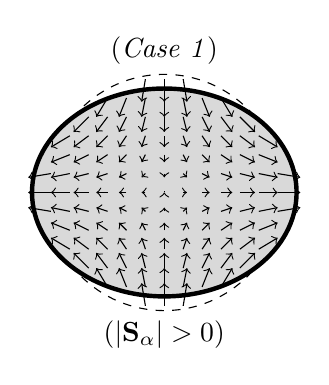
\begin{tikzpicture}[ultra thick,scale=0.6]
        \def\nRows{6}
        \def\nCols{6}
        \draw[dashed,thin] (0,0)circle(2.5);
        \draw[fill=gray!30] (0,0)ellipse(2.8 and 2.2);
        \foreach \x in {-\nRows,...,\nRows} {
            \foreach \y in {-\nCols,...,\nCols} {
                \pgfmathsetmacro\distance{veclen(\x*0.4, \y*0.4)};
                \pgfmathparse{\distance < 2.45 ? "blue" : "white"}
                \edef\colour{\pgfmathresult};
                \ifthenelse{\equal{\colour}{blue}}{                    
                    \draw[thin,->](\x*0.4,\y*0.4)--++(0.08*\x,-0.08*\y);
                }
            }
        }
        \node (txt) at (0,3){(\textit{Case 1})};
        \node (txt) at (0,-3){($|\textbf{S}_\alpha| > 0$)};
    \end{tikzpicture}
     \hfill
    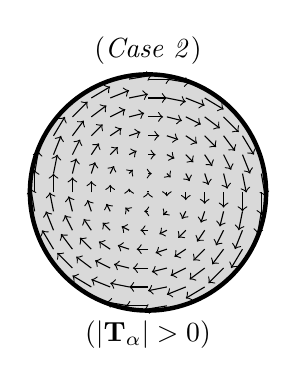
\begin{tikzpicture}[ultra thick,scale=0.6]
        \def\nRows{6}
        \def\nCols{6}
        \draw[fill=gray!30] (0,0)circle(2.5);
        \foreach \x in {-\nRows,...,\nRows} {
            \foreach \y in {-\nCols,...,\nCols} {
                \pgfmathsetmacro\distance{veclen(\x*0.4, \y*0.4)};
                \pgfmathparse{\distance < 2.5 ? "blue" : "white"}
                \edef\colour{\pgfmathresult};
                \ifthenelse{\equal{\colour}{blue}}{                    
                    \draw[thin,->](\x*0.4,\y*0.4)--++(0.08*\y,-0.08*\x);
                }
            }
        }
        \node (txt) at (0,3){(\textit{Case 2})};
        \node (txt) at (0,-3){($|\textbf{T}_\alpha| > 0$)};
    \end{tikzpicture}
    \hfill
    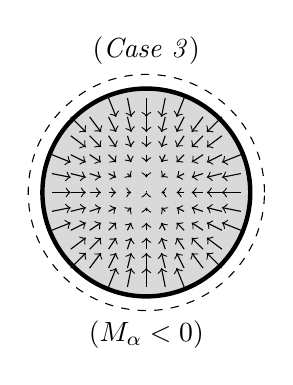
\begin{tikzpicture}[ultra thick,scale=0.6]
        \def\nRows{6}
        \def\nCols{6}
        \draw[dashed,thin] (0,0)circle(2.5);
        \draw[fill=gray!30] (0,0)circle(2.2);
        \foreach \x in {-\nRows,...,\nRows} {
            \foreach \y in {-\nCols,...,\nCols} {
                \pgfmathsetmacro\distance{veclen(\x*0.4, \y*0.4)};
                \pgfmathparse{\distance < 2.3 ? "blue" : "white"}
                \edef\colour{\pgfmathresult};
                \ifthenelse{\equal{\colour}{blue}}{                    
                    \draw[thin,->](\x*0.4,\y*0.4)--++(-0.08*\x,-0.08*\y);
                }
            }
        }
        \node (txt) at (0,3){(\textit{Case 3})};
        \node (txt) at (0,-3){($M_\alpha < 0$)};
    \end{tikzpicture}
    \hfill
    \caption{Graphical representation of the inner kinematics of an arbitrary particle under three scenarios. 
        The arrows represent the velocity field inside the particle, $\textbf{w}_d^0$, with the corresponding value of the moment of momentum tensor indicated below. 
        The operator $|\ldots|$ refers to the norm of the tensors. 
        According to the inner velocity field:
        (\textit{Case 1}) The particle experiences a mean rate of deformation, resulting in non-zero stretching of momentum along the principal axis of deformation;
        (\textit{Case 2}) The particle is rotating, leading to a non-zero angular momentum vector in the direction of rotation;
        (\textit{Case 3}) The particle undergoes compression, resulting in a negative trace of the moment of momentum.
    }
    \label{eq:scheme}
\end{figure}

Injecting, $f_d^0 = \rho_d$ in the second-order moment equation (derived in \ref{ap:Moments_equations}) we obtain :
\begin{equation}
    \ddt {\textbf{M}_\alpha}=2\textbf{S}_\alpha. 
    \label{eq:dt_M_alpha}
\end{equation}
which is the second-order moment of mass conservation equation. 
From \ref{eq:dt_M_alpha} we deduce that the evolution of the distribution of mass of a particle is solely motivated by the stretching of momentum $\textbf{S}_\alpha$. 
This implies that the angular momentum (not to be confused with the angular velocity) plays no role in the evolution of the second moment of mass. 
This is due to the symmetry of the tensor $\textbf{M}_\alpha$, which must be preserved after differentiation with respect to time.
Note that if the particle has a constant $\textbf{M}_\alpha$ under change of reference frame, such as for spherical particles where we can write $\textbf{M}_\alpha= \frac{a^2 m_\alpha}{5} \bm\delta$, then $\textbf{S}_\alpha=0$ since $\ddt \textbf{M}_\alpha = 0$ in this situation.
This argument has no restriction on the internal particle motions, thus it is also true for fluid particles with possible inner motion. 
Additionally, applying the trace operator on both sides of \ref{eq:dt_M_alpha}, yields the interesting relation $\ddt {M_\alpha}=\frac{2}{3}\bm\delta : \textbf{S}_\alpha$.
We can state that $M_\alpha = \lambda^\alpha_1(t)+\lambda^\alpha_d(t)+\lambda^\alpha_3(t)$, with $\lambda_i^\alpha$ for $i=1,2,3$, the eigenvalues of $\textbf{M}_\alpha$, as it is a symmetric tensor and thus always diagonalizable.
For undeformable particles, it is evident that the eigenvalues are not functions of time, implying $\ddt M_\alpha = 0$.  
Consequently, $\bm\delta : \textbf{S}_\alpha$ possesses the notable property of being zero whenever the particle shape remains constant, regardless of the orientation.

Now that we have described the kinematics of the particle shape, let us proceed to derive an equation for the dynamics of the particle shape, i.e. an equation for the moment of momentum. 
This equation is derived injecting $\textbf{Q}_\alpha = \textbf{P}_\alpha$ in \ref{eq:dt_Q_alpha_tot}, it reads, 
\begin{equation}
    \ddt {\textbf{P}_\alpha}
    - \intO{ \rho_d  \textbf{w}_d^0 \textbf{w}_d^0 }
    = 
    - \intO{\bm{\sigma}_d^0}
    - \intS{ 
        \gamma (\bm\delta - \textbf{nn})
    }
    + \intS{ \textbf{r}\bm{\sigma}_f^0\cdot \textbf{n}_d}.
    \label{eq:dt_P_alpha}
\end{equation}
On the left-hands side of \ref{eq:dt_P_alpha} we identify two inertial terms, i.e. the derivative of $\textbf{P}_\alpha$ and the internal velocity term $\intO{\rho_d\textbf{w}_d^0\textbf{w}_d^0 }$.
The inertia of the particle is then balanced by the terms on the right-hand side of the equation, namely: 
the integral of the particle internal stress $\intO{ \bm{\sigma}_d^0}$; 
the integral of the surface tension stress $\intS{ \gamma (\bm\delta- \textbf{nn}) }$; 
and the first moment of the hydrodynamic stress tensor, $\intS{\textbf{r}\bm\sigma_f^0\cdot \textbf{n}}$.
A discussion regarding the physical implications of this equation is provided below. 

The conservation equation of the angular momentum $\bm{\mu}_\alpha$ is obtained by taking the double contracted product of \ref{eq:dt_P_alpha} with $\bm\epsilon$, which gives 
\begin{equation}
    \ddt\bm{\mu}_\alpha
    =  
    % \textbf{t}_\alpha.
    \intS{ \textbf{r} \times \bm{\sigma}_f^0\cdot \textbf{n}_d }
    \label{eq:dt_mu_alpha}
\end{equation}
Notice that every term on the right-hand side of \ref{eq:dt_P_alpha} vanished due to their symmetric nature apart from the shew-symmetric part of the hydrodynamic stress, which is the hydrodynamic torque applied on the particle $\alpha$.
Particularly, the surface tension terms do not appear in the angular momentum balance since $\bm\sigma_I^0 = \gamma (\bm\delta-\textbf{nn})$ is symmetric, which is consistent with the findings of \citet{hesla1993note}. 
As a consequence, the surface tension does not affect the angular momentum regardless of the particle's shape. 
In the literature, it is common to include the torque due to inter-particular interactions in the angular momentum balance, as is done in \citet{jackson1997locally} and \citet{zhang1997momentum}.
In our case note that $\bm{\sigma}_f^0$ contains also short-range interaction forces which can be assimilated to the particle-particle interaction forces.

Taking the double contracted product of \ref{eq:dt_P_alpha} with the tensor $\bm\delta$ and using \ref{eq:dt_M_alpha}, yields directly  
% \begin{equation}
%     \frac{1}{2}\ddt^2 {M_\alpha}
%     - \frac{1}{3}\intO{ \rho_d \textbf{w}_d^0 \cdot \textbf{w}_d^0}
%     = 
%     \intO{p_d^0} 
%     % - \frac{1}{3}\intS{p_f^0 \textbf{r}\cdot \textbf{n}}
%     - \frac{2}{3} \gamma s_\alpha
%     - \frac{1}{3}\intS{p_f^0 \textbf{r}\cdot \textbf{n}}
%     + \frac{1}{3}\intS{\textbf{r}\cdot\bm\tau_f^0\cdot \textbf{n}},
%     \label{eq:dt_D_alpha}
% \end{equation}
\begin{equation}
    \frac{3}{2}\frac{d^2 M_\alpha}{dt^2}
    - \intO{ \rho_d \textbf{w}_d^0 \cdot \textbf{w}_d^0}
    = 
    - \intO{\bm\sigma_d^0:\bm\delta} 
    % - \frac{1}{3}\intS{p_f^0 \textbf{r}\cdot \textbf{n}}
    - \gamma 2 \intS{}
    % - \frac{1}{3}\intS{p_f^0 \textbf{r}\cdot \textbf{n}}
    + \intS{\textbf{r}\cdot\bm\sigma_f^0\cdot \textbf{n}}.
    \label{eq:dt_D_alpha}
\end{equation}
\ref{eq:dt_D_alpha}, corresponds to the isotropic work balance over the volume and surface of the particle. 
According to \ref{eq:dt_D_alpha}, the rate of compression of a particle, denoted by the second derivative of $M_\alpha$ evolves according to : 
the internal inertial term, $\intO{\rho_d \textbf{w}_d^0 \cdot \textbf{w}_d^0 }$;
the particle internal pressure $\intO{\bm\sigma_d^0:\bm\delta}$; 
the surface energy $\gamma\intS{  }$; 
and the trace of the hydrodynamic first moment $\intS{\textbf{r}\cdot\bm\sigma_f^0\cdot \textbf{n}}$.
If one considers spherical particles composed of compressible fluid, \ref{eq:dt_D_alpha} transforms into the Rayleigh-Lamb-Plesset equation. 
In the steady-state regime, this reduces to the Young-Laplace equation, as indicated by the presence of the first three terms on the right-hand side of \ref{eq:dt_D_alpha}. 

\tb{
    As an example we now consider the \textit{Rayleigh-Lamb-Plesset} equation for spherical bubbles with radius $a_\alpha(t)$. 
    As the droplets remain spherical while keeping a constant mass the moment of momentum and inner velocity field can be expressed, 
    \begin{align*}
        M_\alpha
        = \frac{m_\alpha}{5} a^2_\alpha(t),
        && 
        \textbf{w}_d^0
        = \frac{d a_\alpha}{dt}\frac{\textbf{r}}{a_\alpha(t)},
        \label{eq:expr1}
    \end{align*}
    where it is empathized that the radius $a_\alpha(t)$ is time-dependent. 
    The stress inside the bubbles might be expressed as compressible Newtonian fluids with no resistance to shear such that 
    \begin{equation}
        \bm\sigma_d^0 
        = 
        - p_d^0 \bm\delta
        - \lambda_d (\div \textbf{u}_d^0) \bm\delta
        % + \mu_d \left[\grad \textbf{u}_d^0 + (\grad \textbf{u}_d^0)^\dagger\right]
        = 
        - p_d^0 \bm\delta
        - \frac{3 \lambda_d}{a_\alpha} \frac{d a_\alpha}{dt}  \bm\delta
        % + \mu_d \left[\grad \textbf{u}_d^0 + (\grad \textbf{u}_d^0)^\dagger\right]
        \label{eq:StressBubbles}
    \end{equation}
    where $\lambda_d^0$ is the volume viscosity of the dispersed phase. 
    Assuming incompressible Newtonian fluid for the continuous phase and injecting the expressions \ref{eq:StressBubbles} and \ref{eq:expr1} into \ref{eq:dt_D_alpha} yields, 
    \begin{equation}
        \frac{1}{5} \rho_d^0 a_\alpha \frac{d^2 a_\alpha}{dt^2} 
        - 
        \frac{1}{a_\alpha} \frac{d a_\alpha}{dt} 
        \left(
            3 \lambda_d
            + 2 \mu_f 
        \right)
        = 
        +  \frac{1}{v_\alpha}\intO{p_d^0}
        -  \frac{1}{s_\alpha}\intS{p_f^0}
        - \gamma 2 \frac{3}{a}
    \end{equation}
    By expressing the fluid pressure on the surface in terms of the far field pressure (see daniel) one obtain the \textit{Rayleigh-Lamb-Plesset} equation. 
}

Taking the symmetric part of \ref{eq:dt_P_alpha}, and making use of \ref{eq:dt_M_alpha}, yields a dynamical balance equation for $\textbf{M}_\alpha$, namely
% \begin{multline}    
%     \frac{1}{2}\ddt^2{\textbf{M}_\alpha^\text{dev}}
%     - \intO{\left(
%         \rho_d\textbf{w}_d^0 \textbf{w}_d^0
%         - \rho_d\frac{1}{3}(\textbf{w}_d^0 \cdot \textbf{w}_d^0)\bm\delta\right)}
%     =  
%         - \mu_d \intO{\textbf{e}_d^0}
%         - \intS{\gamma\left(\frac{1}{3}\bm\delta-\textbf{nn}\right)}\\
%         + \frac{1}{2}\intS{\left(\textbf{r}\bm\sigma_f^0+ \bm\sigma_f^0\textbf{r} - \frac{2}{3}(\bm\sigma_f^0\cdot \textbf{r})\bm\delta\right)\cdot \textbf{n}}
%     \label{eq:dt_S_alpha}
% \end{multline}
\begin{equation}    
    \frac{1}{2}\frac{d^2 \textbf{M}_\alpha}{dt^2}
    - \intO{ \rho_d  \textbf{w}_d^0 \textbf{w}_d^0 }
    = 
    - \intO{\bm{\sigma}_d^0}
    - \intS{\gamma (\bm\delta - \textbf{nn})}
    + \intS{(\textbf{r}\bm{\sigma}_f^0+\bm{\sigma}_f^0 \textbf{r})\cdot \textbf{n}_d}.
    \label{eq:dt_S_alpha}
\end{equation}
On the left-hand side of \ref{eq:dt_S_alpha}, we recover the symmetric part of the inertial contributions. 
Especially, in opposition to \ref{eq:dt_P_alpha} we could substitute $\textbf{P}_\alpha+\textbf{P}_\alpha^\dagger$ by $\ddt \textbf{M}_\alpha$. 
Consequently, \ref{eq:dt_S_alpha} is a dynamical equation for the droplet mean deformation. 
In our case, only the external contribution $\frac{1}{2}\intS{\textbf{r}\bm\sigma_f^0\cdot \textbf{n}}$ is responsible for the generation of angular momentum, see \ref{eq:dt_mu_alpha}.
Taking the symmetric part of this tensor ultimately removes this contribution. 
Thus, on the right-hand side of \ref{eq:dt_S_alpha}, we identify the terms responsible for the droplet deformation exclusively.
Therefore, \ref{eq:dt_S_alpha} must be interpreted as an equation for the shape of the particle, represented by the tensor $\textbf{M}_\alpha$.

One might immediately recognize that this equation is in fact an extension of Batchelor’s famous result, 
\begin{equation}
    \intO{\bm{\sigma}_d^0}
    + \intS{\gamma(\bm\delta - \textbf{nn})}
    = \frac{1}{2}\intS{(\textbf{r}\bm\sigma_f^0+\bm\sigma_f^0\textbf{r})\cdot \textbf{n}},
    \label{eq:Batchelor}
\end{equation}
but with the consideration of the inertia of the particle.
\ref{eq:Batchelor} is particularly useful to express the unknown internal stress within solid particles (in which case $\gamma = 0$), in terms of surface integral, i.e. the stresslet $\intS{(\textbf{r}\bm\sigma_d^0+ \bm\sigma_d^0\textbf{r})\cdot \textbf{n}}$.
This relation is the main tool used to express the bulk stress of a suspension, it eventually leads to the computation of the famous Einstein equivalent viscosity, upon having a closed expression for the average of $\intS{(\textbf{r}\bm\sigma_d^0+ \bm\sigma_d^0\textbf{r})\cdot \textbf{n}}$ \citep{guazzelli2011}. 
In the inertial case, due to the limited degree of freedom of solid particles, the tensors $\textbf{M}_\alpha$ and the inner velocity field $\textbf{w}_d^0$ are fully determined by \ref{eq:dt_M_alpha} and \ref{eq:dt_mu_alpha}, indicating that $\textbf{M}_\alpha$ and $\textbf{w}_d^0$ can be utilized in \ref{eq:dt_S_alpha} not as unknowns but as source terms. 
Consequently, for solid particles, \ref{eq:dt_S_alpha} must be interpreted as a generalized equation for the undefined stress $\bm\sigma_d^0$ integrated on the volume of the particles.
Whether it is solid or fluid particles \ref{eq:dt_S_alpha} becomes particularly relevant for expressing the averaged stress within an inertial suspension in terms of Lagrangian properties, as discussed in section \ref{sec:averaged_eq}.

It is now clear that if the surface tension forces play no role in the linear and angular momentum equation, it does impact the moment of momentum $\textbf{P}_\alpha$ or more specifically its symmetric part $\textbf{S}_\alpha$.
Thus, the surface tension force impacts the hydrodynamic behavior of a particle solely through its action on $\textbf{S}_\alpha$, which is related to the shape of a particle represented by $\textbf{M}_\alpha$, through \ref{eq:dt_M_alpha}.
In \ref{ap:Moments_equations} we show how to derive the higher-order moment of momentum equations, which can also be viewed as formulas for the higher moments of the internal particle stress distribution. 
It is interesting to mention that in a recent study of \citet{dolata2021faxen} and \citet{zhou2020lamb} they use energy methods and recover the first two moments of momentum equations hidden into another but equivalent form, valid in the Stokes flow regime. 

Hence, the moment of momentum emerges as a quantity of utmost importance for all types of particles with variable shape or volume. In general, the first moments $\textbf{Q}_{\alpha}$ and $\textbf{Q}_{I\alpha}$ hold significant importance when considering particles with high internal gradients, i.e. when $\grad f_d^0$ or $\gradI f_I^0$ are non-negligible at the scale of one particle. 




\section{The hybrid model}
\label{sec:averaged_eq}
Two distinct descriptions can be applied to the dispersed phase, while only one description is applicable to the fluid phase. 
In this section, we derive averaged equations for the dispersed phase using Lagrangian conservation laws. 
Following this, we  discuss the equivalence between the particle or lagrangian averaged equations for the dispersed phase and the averaged equations for the dispersed phase presented in \ref{sec:two-fluid}.


%Two different descriptions are possible for the dispersed phase while one is available for the fluid phase. 
%In this part we first derive averaged equations for the dispersed phase based on Lagrangian conservation laws. 
%Then we provide a complete discussion regarding the equivalence between the "lagrangian" averaged equations for the dispersed phase and the averaged equations governing the dispersed phase presented in \ref{sec:two-fluid}. 
%based on 
%the set of equations just derived and the averaged equations governing the dispersed phase presented in \ref{sec:two-fluid}. 

\subsection{Dispersed phase averaged equations}

In the preceding section, we have described the dispersed phase using a Lagrangian framework. 
However, to ensure consistency with the Eulerian conservation equations that describe the continuous phase, it is necessary to extend the Lagrangian equations to an Eulerian description. 
The approach presented here follows the methodology pioneered by \citep{lhuillier1992ensemble}.
%In the last section, we have described the dispersed phase within a Lagrangian framework.
%However, to be consistent with the Eulerian conservation equations used to describe the continuous phase, we need to extend the Lagrangian equations to an Eulerian description. 
%The strategy exposed here follow the approach pionnered by \citep{lhuillier1992ensemble}.
%In order to achieve this,
We introduce the function $\delta_\alpha$, which is defined as follows, 
\begin{align}
    \delta_\alpha(\textbf{x},\textbf{x}_\alpha(t,\FF)) 
    = \delta(\textbf{x}-\textbf{x}_\alpha(t,\FF)),
    \label{eq:delta_alpha}
\end{align}
where $\delta$ is the Dirac function.
Note that we explicitly note the arguments $(t,\FF)$ to highlight that the position of the particle $\alpha$ is a function of time and of the flow configuration $\FF$.
Applying the chain rule yields \citep{lhuillier1998}%we may write the partial time derivative of $\delta_\alpha$ can be written as
%\begin{equation}
%\frac{\partial \delta_\alpha(\textbf{x},\textbf{x}_\alpha(t,\FF))}{\partial t} 
%=  \frac{\partial \textbf{x}_\alpha}{\partial t} 
%\cdot \frac{\partial \delta_\alpha}{\partial \textbf{x}_\alpha}(\textbf{x},\textbf{x}_\alpha(t,\FF)) .
%\end{equation}
%This leads to the following expression, 
\begin{equation}
    \pddt \delta_\alpha
    + \div (\textbf{u}_\alpha  \delta_\alpha)
    =0,
    \label{eq:dt_delta_alpha}
\end{equation}
where we used the identity, $\frac{\partial \delta_\alpha}{\partial \textbf{x}_\alpha}  = -\grad \delta_\alpha$ and the fact that $\textbf{u}_\alpha(t,\FF)$ is not a function of $\textbf{x}$. 
\ref{eq:dt_delta_alpha} does not apply in scenarios where topological changes occur, such as break-up or coalescence events. 
In these cases, a source term can be introduced on the right-hand side of \ref{eq:dt_delta_alpha}, similar to the approach used in population balance equations, to account for the birth or death of particles \citep{randolph2012theory}.
%It should be noted that \ref{eq:dt_delta_alpha} is not applicable if changes in topology, such as break-up or coalescence events, occur.
%In such cases it is possible, as it is done in population balance equations, to include a source term on the RHS of \ref{eq:dt_delta_alpha} to account for particle birth or death. 
%Multiplying each Lagrangian quantities $\text q_\alpha$ by $\delta_\alpha$ yields the field $\text q_\alpha(t,\FF)\delta_\alpha(\textbf{x},t,\FF)$, which is defined over the entire domain $\Omega$.
%Likewise, for any derivative of Lagrangian quantities, such as $\ddt \text q_\alpha$, we define its corresponding Eulerian field by multiplying $\ddt \text q_\alpha$ with $\delta_\alpha$ and show that :
By multiplying each Lagrangian quantity $\text q_\alpha$​ by $\delta_\alpha$​, we obtain the field $\text q_\alpha(t,\FF)\delta_\alpha(\textbf{x},t,\FF)$, which is defined throughout the entire domain $\Omega$. 
Similarly, for any derivative of a Lagrangian quantity, such as $\ddt \text q_\alpha$​, the corresponding Eulerian field is defined by multiplying $\ddt \text q_\alpha$ with $\delta_\alpha$ 
%This can be expressed as
Given that $\text q_\alpha(t,\FF)$ and $\textbf{u}_\alpha(t,\FF)$ do not depend on \textbf{x}, and by using Equation \ref{eq:dt_delta_alpha}, we obtain
\begin{equation}
    \delta_\alpha \ddt \text q_\alpha
    = \pddt (\delta_\alpha \text q_\alpha)
    + \div (\delta_\alpha \text q_\alpha \textbf{u}_\alpha).
    \label{eq:dt_delta_alpha_q_alpha}
\end{equation}
%where we have used the fact that $\text q_\alpha(t,\FF)$ and $\textbf{u}_\alpha(t,\FF)$ are not function of \textbf{x}, and we made use of \ref{eq:dt_delta_alpha}.
%Now let us consider a domain containing $N$ particles.
%We define what we call the \textit{particle field} of a quantity $\text q_\alpha$, as the sum of the $\delta_\alpha \text q_\alpha$ over all particles in the flow, namely $\displaystyle\sum_{\alpha=0}^N \delta_\alpha \text q_\alpha$.
%Notice that \ref{eq:dt_delta_alpha_q_alpha} remains valid for a sum of fields since derivative and sum operators commute.
Consider a domain containing $N$ particles. We define the \textit{particle field} for a quantity $\text q_\alpha$​ as the sum of $\delta_\alpha \text q_\alpha$ over all particles within the domain, expressed by $\displaystyle\sum_{\alpha=0}^N \delta_\alpha \text q_\alpha$​. 
Note that the formula given by \ref{eq:dt_delta_alpha_q_alpha} remains valid for the sum of such fields, since the operations of differentiation and summation commute.
%In the objective of obtaining averaged equations for the dispersed phase, we introduce the average of $\text q_\alpha$ as  
To obtain the averaged equations for the dispersed phase, we define the particle average of $\text q_\alpha$​ as
\begin{equation}
     n_p \text q_p(\textbf{x},t) = \avg{\sum_\alpha\delta_\alpha \text q_\alpha},
     \label{eq:p_avg}
\end{equation}
where, $n_p(\textbf{x},t) = \avg{\sum_\alpha \delta_\alpha}$ is the probability density of finding a particle center of mass in the infinitesimal volume $d\textbf{x}$ around \textbf{x}, and $\text q_p(\textbf{x},t)$ is the average of $\text q_\alpha$ conditionally on the presence of a particle at \textbf{x} and time $t$. 
To simplify the notations, we consider the shorthand \citep{lhuillier1998},
\begin{equation*}
    \sum_\alpha \delta_\alpha \to \delta_p, 
\end{equation*}
such that $\pavg{\text q_\alpha}=\avg{\sum_\alpha \delta_\alpha \text q_\alpha}=n_p\text q_p$.
Note that we used the subscript $_p$ on $\text q_p$ to denote that this represents a particle-averaged field, initially derived from Lagrangian quantities. 
%Furthermore, in view of equation   
Additionally, in light of \ref{eq:def_fluctu} we define the fluctuating part of a particle field $\text q_p$ as
\begin{equation}
    \text q_\alpha' = \text q_\alpha - \text q_p. 
    \label{eq:def_fluc_p}
\end{equation}

To obtain the particle phase averaged equations one multiply \ref{eq:dt_q_alpha_tot} and \ref{eq:dt_Q_alpha_tot} by $\delta_\alpha$ and apply the ensemble average (\ref{eq:avg}), this yields
\begin{align}
    \pddt (n_p\text Q_p)
    + \div (n_p \text Q_p \textbf{u}_p + \pavg{\textbf{u}_\alpha' \text Q_\alpha'})
    = \pOavg{ s_d^0 }
    + \pSavg{ s_I^0 }\nonumber\\
    + \pSavg{ \left[\mathbf{\Phi}_f^0 + f_f^0 (\textbf{u}_\Gamma^0-\textbf{u}_f^0) \right] \cdot \textbf{n}_d },
    \label{eq:avg_dt_dq_alpha_tot}\\
    \pddt (n_p\textbf{Q}_p^{(1)})
    + \div \left(n_p \textbf{Q}_p^{(1)} \textbf{u}_p + \pavg{\textbf{u}_\alpha' \textbf{Q}_\alpha^{(1)'}}\right)
    =\pOavg{ \left(
        \textbf{r} s_d^0         
        + f_d^0  \textbf{w}_d^0 
        - \mathbf{\Phi}_d^0
    \right) }\nonumber\\
    + \pSavg{ \left(
        \textbf{r}s_\Gamma^0
        + f_\Gamma^0 \textbf{w}_\Gamma^0
        - \mathbf{\Phi}_{\Gamma||}^0
    \right) }
    + \pSavg{ \textbf{r} \left[
        \mathbf{\Phi}_f^0
        + f_f^0 (\textbf{u}_\Gamma^0-\textbf{u}_f^0)
    \right]\cdot \textbf{n}_d  }.
    \label{eq:avg_dt_dQ_alpha_tot}
\end{align}
The derivation of the higher moment particle-averaged equations is provided in \ref{ap:Moments_equations}.
The only fluxes appearing in \ref{eq:avg_dt_dq_alpha_tot} and \ref{eq:avg_dt_dQ_alpha_tot} are the fluctuation tensors $\pavg{\textbf{u}_\alpha' \text q_\alpha'}$ and $\pavg{\textbf{u}_\alpha' \textbf{Q}_\alpha'}$. 
Therefore, the non-convective fluxes $\bm\Phi_d^0$ and $\bm\Phi_I^0$ do not play the role of macroscopic fluxes, as it is the case in \ref{eq:avg_dt_chi_f} and \ref{eq:avg_dt_delta_f}. Instead, they act as source terms in the first moment and higher moment equations. 
This distinction is the main structural differences between the Kinetic-like model (\ref{eq:avg_dt_dq_alpha_tot} and \ref{eq:avg_dt_dQ_alpha_tot}) and the two-phase flow model (\ref{eq:avg_dt_chi_f} and \ref{eq:avg_dt_delta_f}). 
In this study, \ref{eq:avg_dt_chi_f} and \ref{eq:avg_dt_delta_f} are referred to as the phase-averaged equations, while \ref{eq:avg_dt_dq_alpha_tot} and \ref{eq:avg_dt_dQ_alpha_tot} are called the particle-averaged equations. 


 





%\subsubsection*{Equivalence between particle and continuous models}
\subsection{Equivalence between particle-averaged and phase-averaged equations}
\label{sec:equivalence}
%To model the dispersed phase we can either use \ref{eq:avg_dt_chi_f} with $k=d$, or the particle-averaged equations: \ref{eq:avg_dt_dq_alpha_tot}, \ref{eq:avg_dt_dQ_alpha_tot} and possibly the higher moments equations in \ref{ap:Moments_equations}. 
%Consequently, it is fair to address the question of the compatibility and differences between both formalisms. 
To model the dispersed phase, there are two distinct approaches. 
We can either use \ref{eq:avg_dt_chi_f} with $k=d$, or we can employ the particle-averaged equations \ref{eq:avg_dt_dq_alpha_tot}, \ref{eq:avg_dt_dQ_alpha_tot} and potentially the higher moments equations found in \ref{ap:Moments_equations}.
Consequently, it is important to address the compatibility between these two formalisms.
It has been demonstrated in various studies \citep{buyevich1979flow,lhuillier1992ensemble,jackson1997locally,zhang1994averaged}, that phase-averaged quantities can be expressed as a Taylor series expansion of particle-averaged quantities. 

The aforementioned studies used the single-particle conditionally averaged approach to demonstrate this equivalence.  
In this work we use instead the ``distributional'' approach of \citet{pahtz2023general} since, as shown below it yields more general and simpler formulation. 
The dispersed phase indicator function $\chi_d$ can be expressed as a sum of phase indicator function, $\chi_d(\textbf{x},t,\FF) = \sum_\alpha\chi_\alpha(\textbf{x},t,\FF)$ where $\chi_\alpha =1$ in the particle domain $\Omega_\alpha(\FF,t)$ and $0$ otherwise. 
Thus, any dispersed phase quantity pertaining to a single particle can be written as, 
\begin{equation}
   f^0_d \chi_\alpha(\textbf{x},t,\FF)
   = 
   \int_{\mathbb{R}^3} 
    f^0_d \chi_\alpha(\textbf{x}_\alpha + \textbf{r},t,\FF)\delta(\textbf{x} - \textbf{x}_\alpha - \textbf{r}) 
    d\textbf{r} 
   \label{eq:taylor_f_d}
\end{equation}
Likewise, we assume that the interface indicator function $\delta_\Gamma$ can be partitioned into $N$ interface indicator function such that $\delta_\Gamma =  \sum_\alpha  \delta_{\Gamma\alpha}$.
In that case any surface-averaged quantities may be written, 
\begin{equation}
    f_\Gamma^0 \delta_\Gamma(\textbf{x},t,\FF) = 
    \sum_\alpha 
    \int_{\mathbb{R}^3} 
     f_\Gamma^0 \delta_{\Gamma\alpha}(\textbf{x}_\alpha + \textbf{r},t,\FF)\delta(\textbf{x} - \textbf{x}_\alpha - \textbf{r}) 
     d\textbf{r}. 
    \label{eq:taylor_f_I}
\end{equation}
% Notice that \ref{eq:taylor_f_d} and \ref{eq:taylor_f_I} are well-defined in the distributional sense since the integral on the right-hand side of both equations correspond to a convolution product.
Notice that the integral on the right-hand side of \ref{eq:taylor_f_d} and \ref{eq:taylor_f_I} correspond to a convolution product.
Additionally, since the Dirac distribution $\delta(\textbf{x} - \textbf{x}_\alpha - \textbf{r})$, is the unit of convolution \ref{eq:taylor_f_d} is verified (see \citet[Chapter 9]{appel2007}).
The convolution product of the Dirac delta and the derivative of the Heaviside distribution is also well-defined, see \citet[Chapter 9]{appel2007}.
It follows that \ref{eq:taylor_f_d} and \ref{eq:taylor_f_I} are well-defined in the distributional sense. 
Upon using the Taylor expansion of the Dirac delta function $\delta(\textbf{x} - \textbf{x}_\alpha - \textbf{r})$ in the neighborhood of $\textbf{r}=0$ one obtain,
\begin{equation}
\delta(\textbf{x} - \textbf{x}_\alpha - \textbf{r})
= \delta(\textbf{x} - \textbf{x}_\alpha)
- \textbf{r}\cdot\grad \delta(\textbf{x} - \textbf{x}_\alpha)
+ \frac{\textbf{rr}}{2}:\grad\grad\delta(\textbf{x} - \textbf{x}_\alpha) 
- \ldots.
% + \ldots
\label{eq:exp_delta}
\end{equation}
Injecting \ref{eq:exp_delta} into \ref{eq:taylor_f_d} and \ref{eq:taylor_f_I}, and noticing that the indicator functions, $\chi_\alpha$ and $\delta_\Gamma$, reduce the domain of integration from $\mathbb{R}^3$ to, $\Omega_\alpha$ and $\Gamma_\alpha$, respectively,  yields: 
\begin{align}
    f^0_d \chi_d
    =\delta_p\intO{f^0_d}
    - \div\left(\delta_p\intO{\textbf{r} f^0_d}\right)
    + \frac{1}{2}\grad\grad :\left(\delta_p\intO{\textbf{rr} f^0_d}\right)
    \ldots 
    \label{eq:fd_asympt}
   \\
   f_\Gamma^0 \delta_\Gamma 
   =\delta_p\intS{f^0_\Gamma}
   - \div\left(\delta_p\intS{\textbf{r} f^0_\Gamma}\right)
   + \frac{1}{2}\grad\grad :\left(\delta_p\intS{\textbf{rr} f^0_\Gamma}\right)
   \ldots 
   \label{eq:fG_asympt}
%    \\
\end{align} 
Where we recognize the zeroth, first and second order moments of $f_d^0$ and $f_\Gamma^0$, into \ref{eq:fd_asympt} and \ref{eq:fG_asympt}, respectively. 
Notice that even before applying any kind of averaging procedure \ref{eq:fd_asympt} and \ref{eq:fG_asympt} illustrates the connection between the dispersed phase fields, of the form $\chi_d(\ldots)$ or $\delta_\Gamma(\ldots)$, and the particle fields of the form $\delta_p(\ldots)$. 
It is interesting to notice that these relations hold in a distributional sense at a local level. 


Applying similar considerations to the interface indicator function $\delta_\Gamma$, and averaging over all configurations, we obtain the general relations that link continuous-averaged and particle-averaged fields, namely \citep{lhuillier1992ensemble,lhuillier1998,lhuillier2000bilan}, 
\begin{align}
    \avg{\chi_df_d^0} 
    &=  \pavg{\text q_\alpha}
        - \div  
        \pavg{\textbf{q}_\alpha^{(1)}}        
        + \frac{1}{2} \grad\grad : \pavg{\textbf{q}_{\alpha}^{(2)}}
        + \ldots  \label{eq:f_exp_chi} \\
    \avg{\delta_\Gamma  f_\Gamma ^0} 
    &=  \pavg{\text q_{\Gamma \alpha}}        
        - \div \pavg{\textbf{q}_{\Gamma\alpha}^{(1)}}
        + \frac{1}{2} \grad\grad : \pavg{\textbf{q}_{\Gamma\alpha}^{(2)}}
        + \ldots  
    \label{eq:f_exp_delta}
\end{align}
%\JL{j'ai ajoute la sommes des contributions dans les particules et de surfaces}
Summing \ref{eq:f_exp_chi} and \ref{eq:f_exp_delta} we obtain
\begin{equation}
    \avg{\chi_df_d^0+\delta_\Gamma  f_\Gamma ^0} = \pavg{\text Q_\alpha}
    - \div  
    \pavg{\textbf{Q}_\alpha^{(1)}}        
    + \frac{1}{2} \grad\grad : \pavg{\textbf{Q}_{\alpha}^{(2)}}
    + \ldots  \label{eq:f_exp}
\end{equation}
When considering an infinite number of terms in \ref{eq:f_exp} one might eventually obtain a converged approximation of $\avg{\chi_d f_d^0+\delta_\Gamma  f_\Gamma ^0}$. 
However, it is important to note that Taylor series have what is known as a \textit{radius of convergence} beyond which adding more terms does not necessarily improve the approximation \citep[Chapter 1]{appel2007}. 
In particular, for distances beyond a certain limit \textbf{r} the series might diverges depending on the behavior of the function $\avg{\chi_d f_d^0+\delta_\Gamma  f_\Gamma ^0}$ near the point $\textbf{x}$. 
For the purposes of this article, we will assume that the Taylor series has an infinite radius of convergence, although this assumption warrants further investigation.%function $f_d^0$ evaluated at a point $\textbf{x}_\alpha$ is greater than the particle size, then \ref{eq:f_exp} might converges and provides a good approximation.
%\JL{j'ai vraiment raccourci cette partie, car meme si je la trouve pertinente il y a des elements que je trouvais peu claire:
%\begin{itemize}
%\item tu dis que "to assume that $f_d$ is slowly variying at the scale of the particle", justement je ne pense pas que l'on veuille cela car sinon a quoi serve les moments d'ordres superieurs.
%Par ailleurs pr moi (mais peut etre que je me trompe), le rayon de convergence dsun' serie de Taylor n'a rien a voir avec le fait que la fonction dont on cherche la serie varie peu à l'endroit du developpement
%Enfin sur cette idée de precision de la série, pr moi le developpement en série se fait dans l'hypothèse ou la grandeur d'interet (moyennée) varie peut sur l'échelle des grandeurs macroscopiques
%en gros un developpement limite en $a/L$ ou $L$ est la taille des echelles macro.
%\end{itemize}
%}

%In brief, high care must be taken when using these kind of taylor expansion especially in that context since we do not know the exact form of $f_d$.  
%Nevertheless it is reasonable to assume that $f_d$ is slowly variying at the scale of the particle with a radius of convergence sufficiently large, in this case \ref{eq:f_exp} might provide a good approximation, 
%and we might expect an error of $\mathcal{O}[(a/L)^{n}]$ when the highest moment of the series is of order $n-1$ with $L$ being a macroscopic length scale. 
%It is within the context of this assumption that the following disscussion takes place. 

% \JL{pour l'instant j'ai eneleve la partie applicative (meme si elle me semble tres interessante). 
% D'ailleurs pq le second terme du dvt pr les conservation de la masse est nul ? 
% Ce serait bien de donner de petites lois d'echelles pr evaluer les ordres de grandeurs de chacun des termes.}
%Particularly we note that if $f_d^0 = \rho_d$ and $f_d^0 = \rho_d \textbf{u}_d^0$ we obtain, 
%\begin{align}
%    \label{eq:f_exp_exe1}
%    \phi_d \rho_d
%    = m_p n_p 
%    + \frac{1}{2}\grad^2 : (n_p\textbf{M}_p)+\ldots,\\
%    \phi_d \rho_d \textbf{u}_d
%    = m_p n_p \textbf{u}_p 
%    - \div (n_p\textbf{P}_p)+\ldots,
%    \label{eq:f_exp_exe}
%\end{align}
%respectively. 
%Meaning that $\phi_d\rho_d$ is related to the shape of the particles, represented by $\textbf{M}_p$ through \ref{eq:f_exp_exe1}.
%Additionally, considering \ref{eq:f_exp_exe}, it becomes apparent that the phase-averaged velocity $\textbf{u}_d$ encompasses the first moment of momentum $\textbf{P}_p$, which as discussed (in \ref{sec:Lagrangian}) accounts for the rotational, dilatational, and stretching motions of the particles. 
%The second terms on the right-hand side of \ref{eq:f_exp_exe1} and \ref{eq:f_exp_exe} become negligible for homogeneous mixture, i.e. if $n_p$, $\textbf{M}_p$ and $\textbf{P}_p$ are not function of \textbf{x}. 
%Conversely, these terms might become significant if $n_p$, $\textbf{M}_p$ or $\textbf{P}_p$ are space-dependent.
%For example, close to solid boundaries of a macroscopic flow strong gradients of $n_p$ are present at the particle length scale, since at the exact location of the boundaries we must respect $n_p = 0$. 
%In \cite{prosperetti1995finite} they study the importance of these terms, especially their remark that the approximation $\phi \approx n_p v_p$ may have significant consequence on the hyperbolicity of a two-phase flow system. 

To demonstrate the equivalence between the two formalisms, we follow a strategy similar to \citep{lhuillier2000bilan,lhuillier2009rheology}. 
%\JL{j'ai simplifie la description}
%We take the Taylor expansion of each terms in \ref{eq:avg_dt_chi_f} with $k=d$ using the relation \ref{eq:f_exp_chi}. 
%A similar procedure is followed for  the surface transport equations.
%Since we made use of the surface transport equations in the particles phase equations : \ref{eq:avg_dt_dq_alpha_tot} and \ref{eq:avg_dt_dQ_alpha_tot}, we also consider \ref{eq:avg_dt_delta_f} to prove equivalence. 
%As the resulting expression can become quite cumbersome, we will adopt the following definition. 
Let $\mathcal{C}_d$ denote the phase-averaged equation of conservation (\ref{eq:avg_dt_chi_f} with $k=d$) and $\mathcal{C}_\Gamma $ the averaged surface transport equation (\ref{eq:avg_dt_delta_f}).
Specifically, they are defined as follows
\begin{align}
    \mathcal{C}_d
    &=
    - \pddt \avg{\chi_df_d^0}
    - \div \avg{\chi_d \mathbf{\Phi}_d^0 - \chi_df_d^0 \textbf{u}_d^0}
    + \avg{\chi_d s_d^0}
    + \avg{\delta_\Gamma \left[
        \mathbf{\Phi}_d^0
        + f_d^0
        \left(
            \textbf{u}_\Gamma ^0
            - \textbf{u}_d^0
        \right)
    \right]
    \cdot \textbf{n}_d},\\
    \mathcal{C}_\Gamma 
    &= 
    -\pddt \avg{\delta_\Gamma f_\Gamma ^0}
    -\div \avg{\delta_\Gamma  f_\Gamma ^0 \textbf{u}_\Gamma ^0-\delta_\Gamma  \mathbf{\Phi}_{I||}^0 }
    + \avg{\delta_\Gamma s_\Gamma ^0} 
    - \avg{\delta_\Gamma  \Jump{
     \mathbf{\Phi}_k^0+
    f_k^0 (\textbf{u}_\Gamma ^0 - \textbf{u}_k^0)
    } }. 
\end{align}
It should be noted from \ref{eq:avg_dt_chi_f} and \ref{eq:avg_dt_delta_f} that $\mathcal{C}_d\equiv 0$ and $\mathcal{C}_\Gamma  \equiv 0$.
By applying the Taylor expansion to each term of $\mathcal{C}_d+\mathcal{C}_\Gamma $ as described in \ref{eq:f_exp} yields
\begin{equation}
    \mathcal{C}_d 
    + \mathcal{C}_\Gamma  
    = \mathcal{M}^{(0)} - \div \mathcal{M}^{(1)} + \frac{1}{2} \grad\grad : \mathcal{M}^{(2)} \ldots = 0,
    \label{eq:scheme_equivalence}
\end{equation} 
where the expressions for $\mathcal{M}^{(0)}$ and $\mathcal{M}^{(1)}$ are given by 
\begin{align}
    &\mathcal{M}^{(0)}
    = 
    - \avg{\delta_p \ddt {\text Q_\alpha}}
    % -\avg{\delta_p\textbf{u}_\alpha q_\alpha^\text{tot}}
    + \pOavg{ s_d^0 }
    + \pSavg{ s_\Gamma ^0 }
    + \pSavg{ 
    \left[\mathbf{\Phi}_f^0 
    + f_f^0 (\textbf{u}_\Gamma ^0-\textbf{u}_f^0) \right] \cdot \textbf{n}_d },\\
    &\mathcal{M}^{(1)} =
    -  \avg{\delta_p \ddt {\textbf{Q}_\alpha^{(1)}}}
    % - \avg{\delta_p\textbf{u}_\alpha \textbf{Q}_\alpha^\text{tot}}
     + \pOavg{ \left(
        \textbf{r} s_d^0         
        + f_d^0  \textbf{w}_d^0 
        - \mathbf{\Phi}_d^0
    \right) }
    + \pSavg{ \left(
        \textbf{r}s_\Gamma ^0
        + f_\Gamma ^0 \textbf{w}_\Gamma ^0
        - \mathbf{\Phi}_{\Gamma||}^0
    \right) } \nonumber\\
    &+ \pSavg{ \textbf{r} \left[
        \mathbf{\Phi}_f^0
        + f_f^0 (\textbf{u}_\Gamma ^0-\textbf{u}_f^0)
    \right]\cdot \textbf{n}_d  }.
\end{align}
Using \ref{eq:scheme_equivalence}, we reach one of the main conclusion of this study. 
We observe that $\mathcal{M}^{(0)}$ and $\mathcal{M}^{(1)}$ correspond to the zeroth and first-order moment equations, respectively. 
Additionally, as demonstrated in \ref{ap:Moments_equations} the coefficient $\mathcal{M}^{(n)}$ in \ref{eq:scheme_equivalence} represents the $n^{th}$ order moment in the particle-averaged conservation equation. 
From \ref{eq:scheme_equivalence} we conclude that combining \ref{eq:avg_dt_chi_f} for $k=d$ and \ref{eq:avg_dt_delta_f} effectively captures the particle moment equations through a Taylor expansion around the particle center of mass. 
%Thus, it is evident that one can use an arbitrary order of particles moments equations to achieve an arbitrarily accurate description of the dispersed phase, regardless of the properties of the multiphase flow.
Therefore, it is clear that by considering an arbitrary order of particle moments equations, one can achieve a highly accurate description of the dispersed phase.


The particle-averaged equations ($\mathcal{M}^{(0)}$\ldots $\mathcal{M}^{(n)}$) form a system with $n$ equations, one for each moment. 
In contrast, the dispersed phase-averaged equations ($\mathcal{C}_d$ and $\mathcal{C}_\Gamma$) consist of only two equations, which aggregate all the particle-averaged equations. 
This indicates that the particle-averaged formalism provides more information since it yields a separate equation for each moment, as opposed to the phase-averaged equations, which are limited to just two. 
This enhanced level of detail is achieved by considering the topology of the dispersed phase as demonstrated in the previous sections.
%Therefore, the particle-averaged formalism encompasses more information since it provides one equation for each moment, in opposition to the phase averaged equations which are only two. 
%Note that this gain in information has been possible through the consideration of the topology of the dispersed phase. 




%In \ref{ap:Moments_equations} we provide the expression for each $\mathcal{M}_n$ as well as the complete derivation of \ref{eq:scheme_equivalence}. 

%Another approach is to notice that $\mathcal{M}_n=0$ for all $n$ since \ref{eq:dt_Q_n} holds for all $n$. 
%Thus, we can rewrite \ref{eq:scheme_equivalence} such that all moments equations vanish, except $\mathcal{M}_0$ (which is arbitrary), this gives, 
%\begin{equation}
%    \mathcal{C}_d 
%    + \mathcal{C}_\Gamma 
%    = \mathcal{M}^{(0)} = 0.
%    \label{eq:proof2}
%\end{equation}
%This implies that equation \ref{eq:avg_dt_chi_f} with the surface transport equation \ref{eq:avg_dt_delta_f} is rigorously equivalent to \ref{eq:avg_dt_dq_alpha_tot}.
%\citet[Appendix A]{zhang1997momentum} provided evidences that the particle-averaged momentum equation is as legitimate as the phase-averaged momentum equation, which is consistent with \ref{eq:proof2}. 
%Additionally, \citet[Appendix A]{nott2011suspension} derived a similar expression than \ref{eq:proof2}, also in the case of the averaged momentum equation for suspension of solid spherical particles.
%Thus, in light of \ref{eq:proof2}, we generalize the conclusion of these authors and demonstrated that this is also true for all conservation laws regardless of the dispersed phase nature.  
%Considering the Lagrangian equations derived in \ref{sec:Lagrangian} this conclusion is not surprising at all since the phase-averaged and particle-averaged equations are all built on \ref{eq:dt_f_k} and \ref{eq:dt_f_I}.
%However, if one does not consider a proper derivation of the lagrangian balance equations as it is done in \ref{sec:Lagrangian} it might not be as obvious, even if \ref{eq:proof2} should remain true as demonstrated by \citet{zhang1997momentum,nott2011suspension}.
%Nevertheless, it is important to note that the conclusion given by \ref{eq:proof2} is not entirely objective since following the same procedure we could show equally that $\mathcal{C}_d+\mathcal{C}_\Gamma  = -\div\mathcal{M}^{(1)}=0$ and $\mathcal{C}_d+\mathcal{C}_\Gamma  = \frac{1}{2}\grad\grad:\mathcal{M}^{(2)}=0$ and so on. 
%Thus, it is more appropriate to examine the problem from the perspective of \ref{eq:scheme_equivalence}. 
%Namely, the particle-averaged equations ($\mathcal{M}^{(1)}$\ldots $\mathcal{M}^{(n)}$) constitute a system of equations with $n$ equations, one equation for each moment, while the phase-averaged equations ($\mathcal{C}_d$ and $\mathcal{C}_\Gamma$) is a system of two equations made of all the particle-averaged equations.
%Therefore, the particle-averaged formalism encompasses more information since it provides one equation for each moment, in opposition to the phase averaged equations which are only two. 
%Note that this gain in information has been possible through the consideration of the topology of the dispersed phase. 




\subsection{Conservation equations}

Given that the aim of this work is not only to demonstrate the equivalence but also to establish a comprehensive framework for analyzing dispersed two-phase flows, we now present \textit{the hybrid} set of conservation equations.
%Let us assume that we are interested by a macroscopic quantity $f$ that follows \ref{dt_f} at the local scale, (here $f^0$ could be the mass, momentum, concentration of chemical species etc \ldots) . 
The system of equations governing a macroscopic quantity $f$ consists of one equation for the fluid phase, which ensures the conservation of $f_f$ and $n$ equations for the dispersed phase, representing the conservation of the quantities $\textbf{Q}_p^{(n)}$.  
In its most general form, the hybrid description of $f$ can be expressed as
%The system of equations for a macroscopic quantity $f$ is constituted from one equation describing the fluid phase, meaning the conservation of $f_f$ and $n$ equations describing the dispersed phase, i.e. the conservation of the $\textbf{Q}_p^{(n)}$.  
%In all its generality the hybrid description of $f$ may be written,
\begin{align}
    \pddt (\phi_f f_f)
    +\div (\phi_f f_f \textbf{u}_f + \mathbf{\Phi}_f^\text{eff})
    &= 
    \phi_f s_f
    - \pSavg{\left[
        \mathbf{\Phi}_f^0
        + f_f^0
        \left(
            \textbf{u}_\Gamma^0
            - \textbf{u}_f^0
        \right)
    \right]
    \cdot \textbf{n}_d} ,
    \label{eq:avg_hybrid_dt_chi_f}\\
        % \pddt \pavg{[\textbf{Q}_\alpha^{(n)}]_{i_1\ldots i_n}^\alpha}
        % + \div  \pavg{\textbf{u}_\alpha [\textbf{Q}_\alpha^{(n)}]_{i_1\ldots i_n}^\alpha}
        % = \sum_{e=1}^{n} 
        % \pOavg{
        %     \prod^{n}_{\substack{ m=1 \\m \neq e}} r_{i_m} [f_d^0\textbf{w}_d^0  - \bm\Phi_d^0]_{i_e}
        % }\nonumber\\
        % + \pOavg{ \pri{1}{n} (\textbf{s}_d^0)_k }
        % +     
        % \sum_{e=1}^{n} 
        % \pSavg{
        %     \prod^{n}_{\substack{ m=1 \\m \neq e}} r_{i_m} [f_\Gamma^0\textbf{w}_\Gamma^0 - \bm\Phi_{||\Gamma}^0]_{i_e}
        % }
        % + \pSavg{ \pri{1}{n} (\textbf{s}_\Gamma^0)_k }\nonumber\\
        % +\pSavg{ \pri{1}{n} ([\bm\Phi_f^0 + \textbf{f}_f^0 \left(\textbf{u}_\Gamma^0 - \textbf{u}_f^0\right)]\cdot \textbf{n}_d)_k }.
        \pddt (n_p\text Q_p)
        + \div (n_p \text Q_p \textbf{u}_p + \pavg{\textbf{u}_\alpha' \text Q_\alpha'})
        &= \pOavg{ s_d^0 }
        + \pSavg{ s_\Gamma^0 }\nonumber\\
        &+ \pSavg{ \left[\mathbf{\Phi}_f^0 + f_f^0 (\textbf{u}_\Gamma^0-\textbf{u}_f^0) \right] \cdot \textbf{n}_d },
        \label{eq:avg_hybrid_q}
        \\
        \pddt (n_p\textbf{Q}_p^{(1)})
        + \div (n_p \textbf{Q}_p^{(1)} \textbf{u}_p + \pavg{\textbf{u}_\alpha' (Q_\alpha^{(1)})'})
        &=\pOavg{ \left(
            \textbf{r} s_d^0         
            + f_d^0  \textbf{w}_d^0 
            - \mathbf{\Phi}_d^0
        \right) }\nonumber\\
        + \pSavg{ \left(
            \textbf{r}s_\Gamma^0
            + f_\Gamma^0 \textbf{w}_\Gamma^0
            - \mathbf{\Phi}_{I||}^0
        \right) }
        &+ \pSavg{ \textbf{r} \left[
            \mathbf{\Phi}_f^0
            + f_f^0 (\textbf{u}_\Gamma^0-\textbf{u}_f^0)
        \right]\cdot \textbf{n}_d  },
        \label{eq:avg_hybrid_q_1}
        \\\nonumber
        \vdots
\end{align}
where the effective continuous phase non-convective flux term reads 
\begin{align}
    \mathbf{\Phi}_f^\text{eff}
    = \avg{\chi_f f_f' \textbf{u}_f'}
    - \avg{\chi_f \bm\Phi_f^0}
    - \pSavg{\textbf{r}\left[
        \mathbf{\Phi}_f^0
        + f_f^0
        \left(
            \textbf{u}_\Gamma^0
            - \textbf{u}_f^0
        \right)
    \right]
    \cdot \textbf{n}_d}
    + \div[\ldots].
\end{align}
%and \eqref{eq:avg_hybrid_dt_chi_f} is that in
The only difference in the conservation equation for the continuous phase between \eqref{eq:avg_dt_chi_f} and \eqref{eq:avg_hybrid_dt_chi_f} is the expansion of the exchange term $\avg{\delta_\Gamma \left[
    \mathbf{\Phi}_f^0
    + f_f^0
    \left(
        \textbf{u}_\Gamma ^0
        - \textbf{u}_f^0
    \right)
\right]
\cdot \textbf{n}_d}$ into a Taylor series in a similar way to \ref{eq:f_exp_delta}. 
The presence of the terms $\div[\ldots]$ in the expression for  $\mathbf{\Phi}_f^\text{eff}$ suggests that higher-order moments of the interphase exchange term are involved.
Similarly, the ellipsis below \ref{eq:avg_hybrid_q_1} implies that an arbitrary number of dispersed phase moment equations can be introduced. In this format, it becomes evident that the exchange term on the right-hand side of \ref{eq:avg_hybrid_dt_chi_f} is identical to that on the right-hand side of \ref{eq:avg_hybrid_q}. 
Additionally, in the effective flux $\mathbf{\Phi}_f^\text{eff}$ the exchange term from  \ref{eq:avg_hybrid_q_1} appears, and this property continues for higher-order moments.  
Consequently, the zeroth order exchange term in the equation for $\text Q_\alpha^{(0)}$ plays the role of a source term for $f_f$, while the first and higher order exchange terms act as a source into the higher moment equations, and contribute to the effective non-convective fluxes for $f_f$. 



The system of equations presented here offers a clear understanding of the roles of the dispersed phase non-convective flux terms, $\bm\Phi_d$ and $\bm\Phi_\Gamma$, in the particle phase conservation equation. 
As evidenced in \ref{eq:avg_hybrid_q}, $\bm{\Phi}_d$ and $\bm{\Phi}_\Gamma$  do not influence the lowest order particle-phase averaged conservation equation, i.e. the equation of $n_p \text Q_p$. 
However, \ref{eq:avg_dt_chi_f} (for $k = d$) and \ref{eq:avg_dt_delta_f}, show that the phase-averaged quantities $f_d$ and $f_\Gamma$, are affected by the non-convective fluxes at the particle surface and internally, since $\bm{\Phi}_d$ and $\bm{\Phi}_\Gamma$ appear in these equations.
This may seem contradictory at first, but it is important to note that $\bm{\Phi}_d^0$ and $\bm{\Phi}_\Gamma^0$ serve as source terms in the conservation equations for higher moments such as $\textbf{Q}^{(1)}_p$ \ldots $\textbf{Q}^{(n)}_p$, which are related to $f_d$ and $f_\Gamma$ through \ref{eq:f_exp}.
In summary, the non-convective fluxes $\bm{\Phi}_d$ and $\bm{\Phi}_\Gamma$  are not explicitly related to $\text Q_p$, regardless of particle nature or volume fraction. 
Instead, their influence on $\text Q_p$ is mediated through the closure terms in equation \ref{eq:avg_hybrid_q}, which may depend on the higher moments $\textbf{Q}^{(1)}_p$ \ldots $\textbf{Q}^{(n)}_p$ or other higher-order particle-related moments.%\footnote{This is typically the configuration observed in dilute flows of axisymmetric fibers within the Stokes regime. In this regime, the force acting on the fiber (which represents the exchange term in the momentum equation) is dependent on the orientation tensor, which in turn is directly linked to the second-order moment of the mass distribution.}. 
These moments, in turn, explicitly depend on $\bm{\Phi}_d$ and $\bm{\Phi}_\Gamma$ as indicated by \ref{eq:avg_hybrid_q_1}. 
%Consequently, it must be understood that the kinetic-like equations (\ref{eq:avg_dt_dq_alpha_tot}) is formally exact and apply for any type of particle and particle volume fraction, as long as the closure terms are well modeled and that the Taylor expansion used in these expressions reaches a convergence on the scale of the particles as discussed below.
%The reader is invited to interpret this expression for the specific case of the momentum conservation law. 






% 
Now that we reached a clear understanding of the mathematical structures of the averaged two phase flow equation we start to expose the averaged set of equations which constitute the \textit{Hybrid model}. 
As, mentioned in \ref{sec:two-fluid} we consider the mass, momentum and energy for the particles and continuous phase. 
Additionally, to describe higher degree of freedom of the particle shape and momentum, one must consider the second moment of mass and first moment of momentum averaged equations. 
This, makes a total of 10 equations, 6 for the particle phase and 4 for the continuous phase.
This system involves numerous equations and closures terms, it is therefore important to consider in a second step a routine to simplify this system by the consideration of the physical particle degree of freedom.
This; is the subject of the next section.    

\subsection{Continuous phase equations}

The equations for the carrier are basically the same as in the classic to fluid model except that the interfacial terms must be modified in order to have the same form as the dispersed phase equations \citep{jackson1997locally,zhang1994averaged}. 
It is done through the use of \ref{eq:f_exp} which help us to convert the exchange terms of the form of $\avg{\delta_I \ldots }$ appearing in \ref{eq:avg_dt_chi_f} to a series expansion of particle phase  quantity : $\pSavg{\ldots} - \div (\ldots)$. 
Where the first term of this series corresponding to the particle averaged equations exchange term. 
Note that due to the expansion shape of \ref{eq:f_exp} we also see appear higher moments of surface in the fluid phase equations, they will be responsible for the additional fluxes in the fluid phase equation due to the presence particles. 
We start by exposing the . 
The continuous phase primary equations simply derived using the generic expression : \ref{eq:avg_dt_chi_f}, and applying the preceding remarks to the interfacial term. 
The mass, momentum and total energy of the continuous phase yield, 
\begin{align}
    \label{eq:dt_hybrid_rho}
    &\pddt (\phi_1 \rho_1)  
    + \div (
        \phi_1 \rho_1\textbf{u}_1
    )
    = 
    0\\
    \label{eq:dt_hybrid_rhou_1}
    &\pddt (\phi_1 \rho_1\textbf{u}_1)  
    + \div (
        \phi_1 \rho_1\textbf{u}_1\textbf{u}_1
        + \bm{\sigma}_1^\text{eq}
    )
    = 
    \phi_1 \rho_1 \textbf{g} 
    - \pSavg{{\bm{\sigma}_1^0 \cdot \textbf{n}_2}}
    % +\div  \pSavg{{\textbf{r}\bm{\sigma}_1^0 \cdot \textbf{n}_2}}
    \\
    \label{eq:dt_hybrid_rhoE_1}
    &\pddt (\phi_1\rho_1E_1)  
    + \div (
        \phi_1\rho_1E_1\textbf{u}_1
        + \bm{q}_1^\text{eq}
        + \textbf{u}_1 \cdot \bm{\sigma}_1^\text{eq}
        % - \textbf{u}_1^0 \cdot \bm{\sigma}_1^0 
        % + \textbf{q}_1^0
        )
    = 
    \phi_1 \rho_1\textbf{u}_1 \cdot \textbf{g} 
    - \textbf{u}_p \cdot \pSavg{{\bm{\sigma}_1^0 \cdot \textbf{n}_2}}\nonumber \\
    &- \pavg{ \textbf{u}_\alpha' \cdot \intS{  \bm{\sigma}_1^0 \cdot \textbf{n}_2}}
    - \pavg{ \intS{\textbf{w}_2^0 \cdot \bm{\sigma}_1^0 \cdot \textbf{n}_2}}
    + \pSavg{{\textbf{q}_1\cdot \textbf{n}_2}}
    % &\div [    
        % \textbf{u}_p \cdot \pSavg{{ \textbf{r}\bm{\sigma}_1^0 \cdot \textbf{n}_2}}
    % + \pavg{ \textbf{u}_\alpha' \cdot \intS{ \textbf{r} \bm{\sigma}_1^0 \cdot \textbf{n}_2}}
    % + \pavg{ \intS{\textbf{r}\textbf{w}_2^0 \cdot \bm{\sigma}_1^0 \cdot \textbf{n}_2}}
    % - \pavg{ \intS{\textbf{r}  \textbf{q}_1^0 \cdot \textbf{n}_2}}
    % ]
\end{align} 
where we defined the equivalent stress tensor $\bm{\sigma}_1^\text{eq}$ and energy flux $\textbf{q}^\text{eq}_1$ as,
\begin{align}
    \label{eq:sigma_eq_def}
    \bm{\sigma}_1^\text{eq}
    =& 
    \avg{\chi_1\rho_1\textbf{u}_1'\textbf{u}_1'}
    - \phi_1 \bm{\sigma}_1%- n_p \textbf{M}_p
    - \pSavg{{\textbf{r}\bm{\sigma}_1^0 \cdot \textbf{n}_2}}\\
    \textbf{q}_1^\text{eq}
    =&\textbf{q}_1^\text{e} +\textbf{q}_1^\text{k}  \nonumber\\
    \textbf{q}_1^\text{e}
    =& \rho_1 \avg{\chi_1 \textbf{u}_1' e_1'} 
    + \phi_1\textbf{q}_1 
    +\pSavg{{\textbf{r}\textbf{q}_1^0 \cdot \textbf{n}_2}} 
    \nonumber\\
    \textbf{q}_1^\text{k}
    =& \rho_1 \avg{\chi_1 \textbf{u}_1' k_1} 
    - \avg{\chi_1 \textbf{u}_1' \cdot \bm{\sigma}_1^0}
    + (\textbf{u}_1 - \textbf{u}_p)\cdot
    \pSavg{{\textbf{r}\bm{\sigma}_1^0 \cdot \textbf{n}_2}}
    \nonumber\\\nonumber
    &- \pavg{ \textbf{u}_\alpha' \cdot \intS{ \textbf{r} \bm{\sigma}_1^0 \cdot \textbf{n}_2}}
    - \pavg{ \intS{\textbf{r}\textbf{w}_2^0 \cdot \bm{\sigma}_1^0 \cdot \textbf{n}_2}}
\end{align}
It is clear that those equations yield essentially the same as the previous set of equations presented in \ref{sec:two-fluid}.
The only difference is the presence of additional fluxes inside $\bm{\sigma}^\text{eq}_1$ and $\textbf{q}^\text{eq}_1$. 
Especially, one can remark the presence of the first moments of external forces. 
In facts, according to \ref{eq:f_exp} an infinite number of moments is present however we chose to explicit only the first of the series. 

% \tb{introduce the exchange term explain the drag and first moments here, just recall that we already seen them}
% \tb{Insiste on the fact that this formulation is physical and NEW}
In this form of the averaged momentum equation we see appear the terms $\pSavg{\bm{\sigma}_1^0 \cdot \textbf{n}_2}$ which is the total components of the interphase drag force, including the mean pressure gradient of the fluid phase pressure. 
Likewise, $\pSavg{\textbf{r}\bm{\sigma}_1^0 \cdot \textbf{n}_2}$ is the total averaged first moment of force traction, which include the mean fluid phase pressure $p_1$. 
As discussed in \ref{sec:Lagrangian} this terms symmetric and skew symmetric part represent the averaged stresslet and torque on the particles, respectively.  
The latter is responsible for the Einstein viscosity computed in dilute stokes flow regime \citep{guazzelli2011}. 
The exchange term in \ref{eq:dt_avg_rhoE_k} have been decomposed into three exchange terms.
Indeed, after taking the Taylor expansion of $\avg{\delta_I (\textbf{u}^0_2 \cdot \bm{\sigma}_1^0 \cdot \textbf{n}_2)}$  we used the following decomposition on each of the moments :
\begin{align}
    \label{eq:exergysource}
    \pavg{ \intS{\textbf{u}^0_2 \cdot \bm{\sigma}_1^0 \cdot \textbf{n}_2}}
    &= 
    \textbf{u}_p \cdot \pSavg{{\bm{\sigma}_1^0 \cdot \textbf{n}_2}}
    + \pavg{ \textbf{u}_\alpha' \cdot \intS{  \bm{\sigma}_1^0 \cdot \textbf{n}_2}}
    + \pavg{ \intS{\textbf{w}_2^0 \cdot \bm{\sigma}_1^0 \cdot \textbf{n}_2}}\\
    \pavg{ \intS{\textbf{r}\textbf{u}^0_2 \cdot \bm{\sigma}_1^0 \cdot \textbf{n}_2}}
   &= 
    \textbf{u}_p \cdot \pSavg{{\bm{\sigma}_1^0 \cdot \textbf{n}_2}}
    + \pavg{ \textbf{u}_\alpha' \cdot \intS{\textbf{r}  \bm{\sigma}_1^0 \cdot \textbf{n}_2}}
    + \pavg{ \intS{\textbf{r}\textbf{w}_2^0 \cdot \bm{\sigma}_1^0 \cdot \textbf{n}_2}}
\end{align}
In this form the contribution to the energy exchange is now clear. 
The first term on the right hands side of \ref{eq:exergysource} represents the work done by the mean phase relative motion, the second term is the work made by the resultants of the forces and individual particles fluctuating velocity, the last term represent the work made by the local force traction on the particle surface with the surface velocity relative to the particle center of mass velocity.
Same comments can be made for the first order moments. 
The relative importance of these three contribution will be determined in the next section, especially we will see that  it depends highly on the particles' nature. 
To our knowledge, such a decomposition has not been seen in the literature except in \citep[Chapter 2]{scorsim2021particle} where they make similar consideration, but for solid spherical particles.
% It is mainly due to the facts that these equations are often used in the context of two-phase flow modeling, which disregard the equation of the dispersed phase energy. 
We recall that the stress integral $\pSavg{\bm{\sigma}_1^0 \cdot \textbf{n}_2}$ contains contact forces as well, making our model consistent with the latter study. 

As discussed previously, \ref{eq:dt_avg_uk2}, \ref{eq:dt_avg_kk} and \ref{eq:dt_avg_ek} need to be reformulated consistently with the dispersed phase exchange term. 
The mean kinetic energy, pseudo turbulent energy and internal energy equation can be reformulated as, 
\begin{align}
    \pddt (\phi_1 \rho_1u_1^2/2)  
    + \div (
        \phi_1 \rho_1\textbf{u}_1u_1^2/2
        + \textbf{u}_1 \cdot \bm{\sigma}_1^\text{eq}
    )
    = 
     \bm{\sigma}_1^\text{eq} : \grad \textbf{u}_1
    + \phi_1 \rho_1 \textbf{u}_1\cdot \textbf{g} 
    -  \textbf{u}_1\cdot 
        \pSavg{{\bm{\sigma}_1^0 \cdot \textbf{n}_2}} 
        % - \div 
        % \pSavg{{\textbf{r}\bm{\sigma}_1^0 \cdot \textbf{n}_2}} 
        \\
    \label{eq:dt_hybrid_k1}
    \pddt (\phi_1\rho_1k_1)  
    + \div (
        \phi_1\rho_1k_1\textbf{u}_1
        + \textbf{q}_1^\text{k} 
        )
    = 
    - \avg{\chi_1\bm{\sigma}_1^0 : \grad \textbf{u}_1^0}
    - \bm{\sigma}_1^\text{eq} : \grad \textbf{u}_1\nonumber
    - \pavg{ \textbf{u}_\alpha' \cdot \intS{  \bm{\sigma}_1^0 \cdot \textbf{n}_2}}\\
    + (\textbf{u}_1 - \textbf{u}_p)\cdot \pSavg{{\bm{\sigma}_1^0 \cdot \textbf{n}_2}} 
    - \pavg{ \intS{\textbf{w}_2^0 \cdot \bm{\sigma}_1^0 \cdot \textbf{n}_2}} 
    \\
    \label{eq:dt_hybrid_e1}
    \pddt (\phi_1\rho_1e_1)  
    + \div (
        \phi_1 \rho_1e_1\textbf{u}_1
        +
        \textbf{q}_1^\text{e} 
        )
    = 
    \avg{\chi_1\bm{\sigma}_1^0 : \grad \textbf{u}_1^0}
    + \pSavg{{\textbf{q}_1^0 \cdot \textbf{n}_2}} 
\end{align}
Our form of the pseudo turbulent energy equation is consistent with the one of former studies \citep[Chapter 7]{morel2015mathematical}\citep[Chapter 2]{scorsim2021particle}\citet{kataoka1989basic}. 
However, the  decomposition of the exchange term isn't present and the expression of $\textbf{q}_1^k$, which gather the first moments of the work, has not been exposed in the literature in such an explicit form.
The energy exchange between the macroscopic microscopic and internal averaged energy will be detailed in the following, as the energy exchange between phases will be discussed.   


\subsection{Dispersed phase equations}

% Now, we turn our attention to the particle phase equations. 
% \tb{Do i put the surface in or out}
% \subsubsection{Primary equations}

By applying straight ensemble averaging on \ref{eq:dt_m_alpha}, \ref{eq:dt_p_alpha} and \ref{eq:dt_E_alpha} we obtain the particle averaged mass, momentum and energy equation, namely, 
\begin{align}
    \label{eq:dt_hybrid_mp}
    \pddt \left(n_p m_p\right)
    + \div \left(n_pm_p\textbf{u}_p
    \right)
    = 
    0\\
    \label{eq:dt_hybrid_up}
    \pddt \left(n_p m_p \textbf{u}_p\right)
    + \div \left(n_p
    m_p \textbf{u}_p \textbf{u}_p 
    + \bm{\sigma}_p^\text{eq}
    \right)
    = 
    n_p m_p \textbf{g}
    + \pSavg{{\bm{\sigma}_1^0 \cdot \textbf{n}_2}},\\
    \label{eq:dt_hybrid_Ep}
    \pddt(m_p n_pE_p^\text{tot})
    + \div(m_pn_p E_p^\text{tot} \textbf{u}_p 
    + \textbf{q}_p^\text{eq} 
    + \textbf{u}_p \cdot \bm{\sigma}_p^\text{eq})
    =  n_p m_p \textbf{u}_p\cdot  \textbf{g}
    % +  n_p ( \textbf{u}'_1 \cdot \bm{\sigma}_1^0 \cdot \textbf{n}_2)_p^\Sigma
    -  \pSavg{\textbf{q}_1^0 \cdot \textbf{n}_2}\nonumber\\
    + \textbf{u}_p \cdot\pSavg{{\bm{\sigma}_1^0 \cdot \textbf{n}_2}}
    + \pavg{\textbf{u}_\alpha' \cdot\intS{\bm{\sigma}_1^0 \cdot \textbf{n}_2}}
    + \pSavg{{\textbf{w}_2^0 \cdot\bm{\sigma}_1^0 \cdot \textbf{n}_2}}
\end{align}
where we have defined, 
\begin{align*}
    &\bm{\sigma}_p^\text{eq}
    =  m_p\pavg{\textbf{u}_\alpha'\textbf{u}_\alpha'}
    &\textbf{q}_p^\text{eq}
    =\textbf{q}_p^\text{e} 
    +\textbf{q}_p^\text{k}  
    +\textbf{q}_p^\text{w}  
    \\
    &\textbf{q}_1^\text{e}
    = m_p \pavg{\textbf{u}_\alpha' e_\alpha'} 
    &\textbf{q}_p^\text{k}
    = m_p \pavg{\textbf{u}_\alpha' k_\alpha} 
    \\
    &\textbf{q}_p^\text{w}
    = 
     \pavg{\textbf{u}_\alpha'W_\alpha'}
    + \pavg{\textbf{u}_\alpha' s_\alpha' \gamma}.
\end{align*}
We have introduced the internal kinetic energy with $n_pW_p = \pOavg{{\rho_2  (w_2^0)^2/2}}$. 
We recognize that these equations posses indeed the exchange terms corresponding to the fluid phase averaged equations but with opposite sign. 
However, note that in opposition to the fluid phase averaged equations, the first order moments do not appear inside the fluxes of the particles equations. 
Consequently, only the fluctuating quantities plays the role of dissipative fluxes. 
It is noteworthy to mentions that in the total drag force term, $ \pSavg{{\bm{\sigma}_1^0 \cdot \textbf{n}_2}}$ the divergence of a stress is hidden, teh latter represent particles-particles contact forces, \citet{jackson1997locally,zhang1997momentum}. 
One may argue that this is not consistent since this stress would also appear on the fluid phase momentum equation upon the development of the term $\pSavg{\bm{\sigma}_1^0\cdot\textbf{n}_2}$. 
However, this is made consistent if one notice that contact force stress is also present in the first moment $\pSavg{\textbf{r}\bm{\sigma}_1^0\cdot\textbf{n}_2}$ but with opposed sign. 
Likewise, note that in some recent models it is possible to expands the momentum exchange terms, as the sum of a \textit{binary force} and the divergence of a stress accounting for particles' long range interaction forces \citep{zhang2021ensemble,nott2011suspension}. 
In opposition to the contact stress, this long range interaction stress, appears on the particle and carrier fluid momentum conservation equation. 
Eventhrougth, the latter stress has been shown to be indispensable to ensure the hypertonicity of the two phase flow equations\citep{fox2020hyperbolic}, we choose to not explicitly display this kind of stresses for succinctness. 

% \subsubsection{Secondary equations}

The particle averaged total energy can be decomposed in the similar way than the continuous averaged total energy \ref{eq:E_def}. 
The decomposition is somewhat more involving than the continuous phase and reads as, 
\begin{equation*}
    n_p m_p E_p(t) 
    = m_p n_p e_p 
    + n_p W_p
    % + n_p s_p \gamma
    + m_p n_p k_p
    + m_p n_p (u_p)^2/2
    \label{eq:E_p_def}
\end{equation*}
The total energy of the particle phase is made of the internal energy $e_p$, the internal kinetic energy $W_p$, the granular temperature $n_p k_p =\pavg{\textbf{u}_\alpha \cdot\textbf{u}_\alpha}/2$ and the kinetic energy of the mean particle phase velocity. 
The mean surface energy $n_p s_p \gamma$ is treated as a source terms in the following equations, that is why it doesn't appear in \ref{eq:E_p_def}.  
If one wish to solve for every component of the energy it is therefore needed to derive two supplementary equation. 
Applying the average procedure on \ref{eq:dt_e_alpha}, \ref{eq:dt_w2_alpha} and \ref{eq:dt_u2_alpha} one can derive an equation for the particle averaged internal energy, internal kinetic energy and mean kinetic energy, it yields, 
\begin{align}
    % &\pddt \left(n_p m_p u_p^2/ 2\right)
    % + \div \left(n_p
    % m_p u_p^2/ 2 \textbf{u}_p 
    % + \textbf{u}_p \cdot \bm{\sigma}_p^\text{eq}
    % \right)
    % = 
    % + \bm{\sigma}_p^\text{eq}  :\grad \textbf{u}_p
    % +  n_p v_p \textbf{u}_p \cdot 
    % \rho_2 \textbf{g}
    % + n_p \textbf{u}_p \cdot (\bm{\sigma}_1^0 \cdot \textbf{n}_2)^\Sigma_p,\\
    \label{eq:dt_hybrid_u2p}
    \pddt \left(n_p m_p (u_\alpha^2)_p/ 2\right)
    + \div \left(n_p
    m_p (u_\alpha^2)_p/ 2 \textbf{u}_p 
    + \textbf{q}^k_p
    + \textbf{u}_p \cdot \bm{\sigma}_p^\text{eq}
    \right)
    = 
    n_p m_p \textbf{u}_p \cdot
    \textbf{g}\nonumber\\  
    + \textbf{u}_p\cdot\pSavg{{\bm{\sigma}_1^0 \cdot \textbf{n}_2}}
    + \pavg{\textbf{u}_\alpha'\cdot\intS{\bm{\sigma}_1^0 \cdot \textbf{n}_2}}
    \\
    \label{eq:dt_hybrid_Wp}
    \pddt \left(n_p W_p\right)
    + \div 
    (n_p W_p
    \textbf{u}_p 
    +  \textbf{q}_p^\text{w}
    )
    = 
    - \pOavg{{\bm{\sigma}_2^0 : \grad\textbf{u}_2^0}}
    + \pSavg{{\textbf{w}_2^0 \cdot \bm{\sigma}_1^0 \cdot  \textbf{n}_2}}
    - \pavg{\dot{ s_\alpha}}
    \\
    \pddt \left(n_p m_p e_p\right)
    + \div \left(n_p
    m_p e_p \textbf{u}_p 
    +  \textbf{q}_p^\text{e}
    \right)
    = 
    + \pOavg{{\bm{\sigma}_2^0 : \grad\textbf{u}_2^0}}
    - \pSavg{{\textbf{q}_1^0\cdot \textbf{n}_2}}
    \label{eq:dt_hybrid_ep}
\end{align}
The center of mass kinetic energy can be further decomposed such as $\pavg{u_\alpha^2}/2 = n_p k_p + n_p u_p^2/2$. 
Then, to derive an equation for $k_p$ one must retrieve to \ref{eq:dt_hybrid_u2p} the dot product of \ref{eq:dt_hybrid_up} with $\textbf{u}_p$, which eventually yields an equation for the mean kinetic energy and another for the granular temperature $k_p$, namely,
\begin{align}
    \label{eq:dt_hybrid_up2}
\pddt \left(n_p m_p u_p^2/ 2\right)
    + \div \left(n_p
    m_p u_p^2/ 2 \textbf{u}_p 
    + \textbf{u}_p \cdot \bm{\sigma}_p^\text{eq}
    \right)
    = 
    \bm{\sigma}_p^\text{eq}  :\grad \textbf{u}_p
    +  n_p m_p \textbf{u}_p \cdot 
     \textbf{g}
    + \textbf{u}_p \cdot \pSavg{{\bm{\sigma}_1^0 \cdot \textbf{n}_2}},\\
    \label{eq:dt_hybrid_kp}
    \pddt \left(n_p m_p k_p\right)
    + \div \left(n_p
    m_p k_p \textbf{u}_p 
    + \textbf{q}^k_p
    % + \textbf{u}_p \cdot \bm{\sigma}_p^\text{eq}
    \right)
    = 
    - \bm{\sigma}_p^\text{eq}  :\grad \textbf{u}_p
    + \pavg{\textbf{u}_\alpha'\cdot\intS{\bm{\sigma}_1^0 \cdot \textbf{n}_2}},
\end{align}
respectively.
Since equation \ref{eq:dt_hybrid_Wp}, \ref{eq:dt_hybrid_ep} and \ref{eq:dt_hybrid_u2p} are discussed in \ref{sec:Lagrangian} let's focus in the granular temperature equation. 
The usual way to derive the granular temperature equations is by the use of kinetic theory, see \citet[Chapter 7 and 9]{rao2008introduction} equation (7.75). 
To bridge the usual formulation of the equation for $k_p$ with the kinetic theory and our model, we remark that the term $\pSavg {\bm{\sigma}_2^0 \cdot \textbf{n}_2}$ takes in account both hydrodynamic forces and particle interaction forces. 
Consequently, the second term on the right hands side of \ref{eq:dt_hybrid_kp} can be decomposed into a contribution due to particle-particle interactions and a contribution due to particle fluid interactions, the former is the dissipation term of see \citet[Chapter 7 and 9]{rao2008introduction} equation (7.75). 
Also, a term written as the divergence of a stress is in fact included in kinetic theory, it is supposed to account for fluxes of granular agitation due to particle-particle elastic interactions. 
This terms can be recovered from the exchange term $\pavg{\textbf{u}_\alpha'\cdot\intS{\bm{\sigma}_1^0 \cdot \textbf{n}_2}}$ with a similar procedure than the derivation of the contact stress tensor, see \citet{scorsim2021particle}. 
Consequently, if we Except that the particles-fluid interaction terms are disagreed such as in \citet{rao2008introduction} we obtain consistent results. 
Notice that we did not make any hypothesis so far, consequently, \ref{eq:dt_hybrid_kp} itself is valid regardless of the particles nature and concentration.
The hypothesis made in kinetic theory are in fact needed to derive the closure for the exchange term, $\pavg{\textbf{u}_\alpha'\cdot\intS{\bm{\sigma}_1^0 \cdot \textbf{n}_2}}$. 

\subsection{The energy exchanges}

One can verify that summing \ref{eq:dt_hybrid_ep}, \ref{eq:dt_hybrid_Wp} and \ref{eq:dt_hybrid_kp} and \ref{eq:dt_hybrid_up2} makes \ref{eq:dt_hybrid_Ep}.  
Under this form it is easy to observe the exchange terms which drive the energy transfer between each component of the total energy. 
Firstly, the source term $\bm{\sigma}_p^\text{Re} :\grad \textbf{u}_p$ appear in \ref{eq:dt_hybrid_up2} and \ref{eq:dt_hybrid_k1} with opposite sign. 
Consequently, macroscopic kinetic energy is transmitted to granular agitation through the macroscopic diffusion scalar : $\bm{\sigma}_p^\text{Re} :\grad \textbf{u}_p$. 
Then between \ref{eq:dt_hybrid_Wp} and \ref{eq:dt_hybrid_ep} we already observed that the source terms is the dissipation term,  $\pOavg{\bm{\sigma}_2^0:\grad \textbf{u}_2^0}$.
However, note that no common term is present between \ref{eq:dt_hybrid_kp} and \ref{eq:dt_hybrid_Wp} which implies that there is no direct transfer of energy between the center of mass velocity fluctuation quantified by $k_p$ and the internal velocity fluctuation energy $W_p$. 
However, notice that the transport equation for $k_1$, \ref{eq:dt_hybrid_k1}, contains the terms $\pavg{\textbf{u}_\alpha' \intS{\bm{\sigma}_1^0 \cdot \textbf{n}_2}}$ and $\pSavg{\textbf{w}_2^0 \cdot \bm{\sigma}_1^0 \cdot \textbf{n}_2}$ which are also present in \ref{eq:dt_hybrid_kp} and \ref{eq:dt_hybrid_Wp}. 
Consequently, the energy transfer from granular agitation $k_p$ and the internal kinetic energy $W_p$ is done through the fluid phase pseudo turbulent kinetic energy. 
To summarize this quite complicated energy cascade between both phases and the different scales we propose the following diagram \ref{fig:energy}. 
\begin{figure}[h!]
    \centering
    \tikzstyle{quadri}=[rectangle,draw]
    \begin{tikzpicture}[scale=1.2]
        \node[quadri] (u2) at (0,0){$(u_p)^2 / 2$};
        \node[quadri] (kp) at (4,0){$(k_p)$};
        \node[quadri] (Wp) at (8,0){$(W_p)$};
        \node[quadri] (ep) at (12,0){$(e_p)$};
        \node[quadri] (u12)at (0,-3){$\frac{\rho_1}{2}(u_1)^2$};
        \node[quadri] (k1) at (6,-3){$k_1$};
        \node[quadri] (e1) at (10,-3){$e_1$};
        \draw[->] (u2)--(kp)node[midway,above]{\footnotesize $\bm{\sigma}^\text{eq}_p:\grad \textbf{u}_1$};
        % \draw[<->,text width=2cm] (kp)--(u12) node[midway,left]{\footnotesize $+  n_p v_p \textbf{u}_p \cdot 
        % (\rho_2 \textbf{g} - \grad p_1)
        % + n_p \textbf{u}_p \cdot \textbf{f}_{pm} - \textbf{F}_\text{pfp}$};
        \draw[<->] (k1)--(u12) node[midway,above]{\footnotesize $\bm{\sigma}^\text{eq}_1:\grad \textbf{u}_1$}node[midway,below,sloped]{\footnotesize $\textbf{u}_1\cdot\pSavg{\bm{\sigma}_1^0\cdot \textbf{n}_2} $};
        \draw[<->] (k1)--(e1) node[midway,below]{\footnotesize $\avg{\chi_1 \bm{\sigma}_1^0 : \grad \textbf{u}_1^0}$};
        \draw[<->,sloped] (k1)--(kp) node[midway,above]{\footnotesize $\pavg{ \textbf{u}_\alpha'\cdot \intS{\bm{\sigma}_1^0\cdot\textbf{n}_2}}$};
        \draw[<->] (k1)--(u2) node[midway,below,sloped]{\footnotesize $\textbf{u}_p\cdot \pSavg{\bm{\sigma}_1^0 \cdot \textbf{n}_1}$};
        \draw[<->,sloped] (k1)--(Wp) node[midway,below]{\footnotesize $\pSavg{{\textbf{w}_2^0 \cdot \bm{\sigma}_1^0\cdot \textbf{n}_1}}$};
        % \draw[->] (kp)--(Wp)node[midway,above]{$(\textbf{u}_\alpha' \cdot \textbf{f}_\alpha')_p$};
        \draw[->] (Wp)--(ep)node[midway,above]{\footnotesize $\pOavg{\bm{\sigma}_2^0 : \grad \textbf{u}_2^0}$};
        \draw (e1)--(ep)node[midway,above,sloped]{\footnotesize $\pSavg{\textbf{q}_1^0 \cdot \textbf{n}_2}$};
    \end{tikzpicture}
    \caption{Energy exchange between the different components of energy in a dispersed two phase flow.
    Macroscopic kinetic energy of the particle phase, $u_p^2/2$, and of the carrier fluid $u_1^2/2$.
    $k_1$, Pseudo turbulent energy of the carrier fluid. 
    $k_p$, Pseudo turbulent energy of particle center of mass. 
     }
    \label{fig:energy}
\end{figure}
% Consequently, the energy gain due to internal dissipation stress $\pOavg{\bm{\sigma}_2^0:\grad \textbf{u}_2^0}$ comes from the internal velocity fluctuation equation. 
In the literature, it is said that the transfer terms between internal energy $e_p$ and the granular temperature $k_p$ is the \textit{dissipation rate} due to inelastic particle-particle collision present in \ref{eq:dt_hybrid_up2}, see for example \citet{fox2014multiphase,rao2008introduction}. 
However, in light of \ref{fig:energy} the energy gain due to  $\pOavg{\bm{\sigma}_2^0:\grad \textbf{u}_2^0}$ which is the \textit{dissipation rate} has no reason to be equal to the energy loss in \ref{eq:dt_hybrid_up2} represented by the term $\pavg{\textbf{u}_\alpha' \intS{\bm{\sigma}_1^0 \cdot \textbf{n}_2}}$. 
In fact some energy is first transmitted to the fluid phase $k_p$, then some of this energy is transmitted to the internal kinetic energy $W_p$, which will induce viscous dissipation within the particle. 
In short, the internal kinetic energy is transformed into internal energy but by no means the \textit{dissipation rate} $\pOavg{\bm{\sigma}_2^0:\grad \textbf{u}_2^0}$ makes the link between to the granular temperature $k_p$ and the internal energy of the particle phase $e_p$. 

\subsection{The first order momentum and mass equations}

As it is suggested in the previous section, the needs for higher moments equations arise if one of the closure terms present in the previous set of equation is highly dependent on one of the moments of the particles. 
In our case we suppose that the second order description of the averaged shape, i.e. $\mathcal{M}_p$, and a first order description of velocity distribution, i.e. $\mathcal{P}_p$,  is enough to express all closure terms. 
By applying the average operator on \ref{eq:dt_M_alpha},\ref{eq:dt_S_alpha} and \ref{eq:dt_mu_alpha}, one get the second order moment of mass, and first order moment of momentum symmetric and skew symmetric parts, namely, 
\begin{align}
    &\pddt \left(n_p \mathcal{M}_p\right)
    + \div \left(
        n_p \textbf{u}_p \mathcal{M}_p
    + \mathcal{M}_p^\text{Re}
    \right)
    =
    n_p2  \mathcal{S}_p
    \label{eq:dt_hybrid_Mp}
    \\
    % \label{eq:dt_hybrid_Pp}
    % \pddt \left(n_p \mathcal{P}_p\right)
    % + \div \left(
    %     n_p \textbf{u}_p \mathcal{P}_p
    % + \mathcal{P}_p^\text{Re}
    % \right)
    % &=
    % % -n_p v_p p_1 \textbf{I}
    % % + n_p \textbf{F}_p
    % \pSavg{
    %     \textbf{r} \bm{\sigma}_1^0 \cdot\textbf{n}_2
    % }
    % + \pOavg{
    %     \rho_2 \textbf{w}_2^0  \textbf{w}_2^0 
    %     - \bm{\sigma}_2'
    % }
    % -  \pSavg{\gamma (\textbf{I} - \textbf{nn})},\\
\label{eq:dt_hybrid_Sp}
&\pddt \left(n_p \mathcal{S}_p\right)
+ \div \left(
    n_p \textbf{u}_p \mathcal{S}_p
+ \mathcal{S}_p^\text{Re}
\right)
=
% -n_p v_p p_1 \textbf{I}
\pSavg{(\textbf{r}\bm\sigma_1^0+\bm\sigma_1^0\textbf{r})\cdot \textbf{n}_2}
% n_p  \mathscr{S}_p^*
% + \pSavg{
%     \textbf{r} \bm{\sigma}_1^0 \cdot\textbf{n}_2
% }
&+ \pOavg{
    \rho_2 \textbf{w}_2^0  \textbf{w}_2^0 
    - \bm{\sigma}_2
}
-  \pSavg{\gamma \textbf{I}_{||}},
\\
\label{eq:dt_hybrid_mup}
&\pddt \left(n_p \bm{\mu}_p\right)
+ \div \left(
n_p \textbf{u}_p \bm{\mu}_p
+ \bm{\mu}_p^\text{Re}
\right)
=
% n_p \textbf{t}_p
\pSavg{\textbf{r}\times(\bm\sigma_1^0\cdot \textbf{n}_2)}
% \label{eq:dt_hybrid_Dp}
% \pddt \left(n_p \mathcal{D}_p\right)
% + \div \left(
%     n_p \textbf{u}_p \mathcal{D}_p
% + \mathcal{D}_p^\text{Re}
% \right)
% &=
% + n_p \textbf{D}_p
% + \pOavg{
%     \rho_2 \textbf{w}_2^0 \cdot  \textbf{w}_2^0 
%     - \bm{\sigma}_2 : \textbf{I}
% }
% + 2 \pSavg{\gamma},
\end{align}
respectively, where we have defined the fluctuaiton terms as $
 \mathcal{M}_p^\text{Re}
 = \pavg{\mathcal{M}_\alpha' \textbf{u}_\alpha'} $,  $ 
 \mathcal{S}_p^\text{Re}
 = \pavg{\mathcal{P}_\alpha' \textbf{u}_\alpha'}$ and $ 
 \bm{\mu}_p^\text{Re}
 = \pavg{\bm{\mu}_\alpha' \textbf{u}_\alpha'}
$.
Note many comments can be made about these equations as they have been already treated in \ref{sec:Lagrangian}. 
However, it is interesting to discuss the case of infinitely rigid particles where the internal velocity is defined by $\textbf{w}_2^0 = \bm\Omega_\alpha \cdot \textbf{r}$ and the particle internal stress is undefined. 
In this case \ref{eq:dt_hybrid_Mp} and \ref{eq:dt_hybrid_mup} might be used to solve for the orientation and angular velocity of the particles. 
Therefore, \ref{eq:dt_hybrid_Sp} seems to be redundant and is in practice never used. 
In fact this equation can be used to determine the averaged stress, $\pOavg{\bm{\sigma}_2}$ in terms of the particles' kinetic properties. 
Knowing the internal stress of the particles, and the constitutive law of the solid material, one is able to compute the averaged deformation of the particle. 
Once the deformation is obtained, one is able to validate, or not, the assumption of infinitely rigid particles made at the origin. 



\subsection{The fluid phase equivalent stress}
\tb{This section can be shortened a lotsss }
% In this section we focus on the formulation of the averaged fluid phase equivalent stress tensor $\bm{\sigma}_1^\text{Re}$. 
For instance the stress appearing on the left hands side of the fluid phase momentum balance is of the form of \ref{eq:sigma_eq_def}. 
However, it is more convenient to express the equivalent stress as a Newtonian stress, plus a contribution arising due to the presence of the particles. 
We first reformulate $\bm{\sigma}_1$ by considering that the carrier fluid is Newtonian, therefore $\phi_1 \bm{\sigma}_1 = - \phi_1 p_1 + \phi_1 \mu_1 \textbf{e}_1$ where $\phi_1 \bm{e}_1 = \avg{\chi_1  (\grad \textbf{u}_1^0 + (\grad \textbf{u}_1^0)^T)}$. 
Additionally, we state that the fluid strain is equal to the bulk strain $\textbf{e} = \grad \textbf{u}+ (\grad \textbf{u})^T$, minus the particle averaged strain, i.e. $\phi_1 \mu_1 \textbf{e}_1 = \mu_1\textbf{e} - \mu_1 \phi_2 \textbf{e}_2$. 
Under this form we clearly remark that $\phi_2 \textbf{e}_2 = 0$ for solid particles, recovering the expression $\phi_1 \textbf{e}_1 = \textbf{e}$ of \citet{jackson1997locally}. 
Upon developing $\phi_2 \textbf{e}_2$ multipolar series, the equivalent stress of the fluid phase can be reformulated as, 
\begin{multline}
    \bm{\sigma}^\text{eq}_1 = 
    \rho_1\avg{\chi_1\textbf{u}_1'\textbf{u}_1'} 
    + \phi_1 p_1 \textbf{I} 
    - \mu_1 \textbf{e} 
    - \pSavg{\textbf{r}\bm{\sigma}_1^0\cdot \textbf{n}_2}
    + \mu_1 \pOavg{\textbf{e}_2^0}\\
    + \frac{1}{2} \div \left[
        \pSavg{\textbf{rr}\bm{\sigma}_1^0\cdot \textbf{n}_2}
        + 2\pOavg{\mu_1 \textbf{re}_2^0 }
        + \ldots
    \right]
    \label{eq:sigma_eq_0}
\end{multline} 
Already, we can see that the equivalent stress of the fluid phase is the made of the average fluid stress represented by the two first terms on the right hands side of \ref{eq:sigma_eq_0}. 
The first moment $\pSavg{\textbf{r}\bm{\sigma}_1^0 \cdot \textbf{n}_2}$ appearing in \ref{eq:sigma_eq_0} posses a skew-symmetric part and a symmetric part, the latter corresponding to the stresslet (see \ref{eq:stresslet_def}).
However, for non-solid particles \ref{eq:stresslet_def} is not entirely valid since in stokes theory the quantity referred as the stresslet is defined as \citet{pozrikidis1992boundary,kim2013microhydrodynamics},
\begin{equation}
    \label{eq:stresslet_def}
    n_p \mathscr{S}_{p,ki}
    = \frac{1}{2}
    \pSavg{
        x_k \sigma_{il}n_l + x_i \sigma_{kl}n_l 
        - \delta_{ik}
        \frac{2}{3}
        x_l \sigma_{lk}n_k
        - 2 \mu_f (u_k n_i+u_i n_i)
    }
\end{equation}
Likewise, we introduce the average skew symmetric part $\mathscr{L}_p$ and the average trace of the first moments $\mathscr{D}_p$ such as, 
\begin{align}
    \label{eq:torque_def}
    n_p \mathscr{L}_{p,ki}
    = \frac{1}{2}\pSavg{ x_k \sigma_{il}n_l - x_i \sigma_{kl}n_l }\\
    \label{eq:trace_def}
    n_p \mathscr{D}_{p,ij}
    = \frac{1}{3}\pSavg{ x_k (\sigma_{kl} + p_1 \delta_{kl})n_l } \delta_{ij}
    - n_p v_p p_1 \delta_{ij}
\end{align}
where we have retrieved the mean pressure from the trace of the first moments, so that we make appear the hydrostatic pressure  $n_p v_p p_1 \textbf{I}$ explicitely.  
Notice that the volume fraction $\phi_1$ is present in front of the averaged pressure terms in \ref{eq:sigma_eq_0}.  
In various study \citep{prosperetti2009computational,chu2016flux}, this term is shown to be problematic  since it might generate nonphysical flux of momentum. 
However, shown above and pointed out by  \citet{zhang1997momentum,jackson1997locally}, the first moment of hydrodynamic force tensor contains a part of the hydrostatic pressure.
With that contribution the total pressure in the fluid stress reach $\phi_1p_1 + n_p p_1 \approx p_1$ which is consistent.
Additionally, as seen in \ref{sec:two-fluid} the Reynolds stress is related to the pseudo turbulent kinetic energy through $\avg{\chi_1 \rho_1\textbf{u}_1'\textbf{u}_1'} : \textbf{I} = 2k_1$ . 
Therefore, we can write, $\avg{\chi_1 \rho_1\textbf{u}_1'\textbf{u}_1'} = 2 \rho_1 k_1 \textbf{I} + \avg{\textbf{u}_1'\textbf{u}_1'}^\text{dev}$ where the second term is the deviatoric part of the Reynolds stress. 

These remarks motivate us to rewrite the equivalent fluid phase stress under the general expression,  
\begin{multline*}
    \bm{\sigma}_1^\text{eq}
    = 
    \underbrace{p_1  \textbf{I}
    - \mu_1 \textbf{e} }_\text{Newtonian fluid stress}
    +  \underbrace{\phi_1 k_1 \textbf{I}
    + \rho_1 \avg{\chi_1\textbf{u}_1'\textbf{u}_1'}^\text{dev}}_\text{fluctuating stresses}
    - \underbrace{(n_p \mathscr{S}_p
    + n_p \mathscr{L}_p
    + n_p \mathscr{D}_p )}_\text{particles stresses}\\
    % + \mu_1  \pSavg{{\textbf{u}_1\textbf{n}_2 + \textbf{n}_2 \textbf{u}_1}}
    % - n_p \textbf{F}_\text{p}
    % + n_p \textbf{F}_\text{pfp} 
    + \frac{1}{2} \div \underbrace{\left[
        \pSavg{\textbf{rr}\bm{\sigma}_1^0\cdot \textbf{n}_2}
        + 2\pOavg{\mu_1 \textbf{re}_2^0 }
        + \ldots
        \right]
        }_\text{inhomogeneous particles stresses}
    \label{eq:sigma_eq1_def}
\end{multline*}
% with, 
% \begin{equation*}
%      \bm{\Sigma}
%     = 
%      \pMSavg{\textbf{rr} \bm{\sigma}_1^0\cdot \textbf{n}_2}
%      -\pMOavg{\mu_1 \textbf{r} \textbf{e}_2 }\\
% \end{equation*}
The contribution of the fluid phase equivalent pressure is made of,
the averaged $p_1$, the fluctuating part of the moment of force traction $\mathscr{D}_p$, and the fluid pseudo turbulent energy, $\phi_1 k_1$. 
The deviatoric part of the stress is constituted of the deviatoric part of the Reynolds stress $\avg{\chi_1\textbf{u}_1'\textbf{u}_1'}^\text{dev}$, the mean fluid shear rate $\mu_1 \textbf{e}$, the stresslet $\mathscr{S}_p$ and the hydrodynamic torque $\mathscr{L}_p$. 
The higher order moments found in $\bm{\Sigma}$ are not necessarily negligible, as shown in \citet{lhuillier1996contribution,jackson1997locally}, in fact they exhibit a different physical meaning. 
The first order moments will be function of the mean gradient of the fluid velocity while the other will be function of the background relative motion. 

It is known that the $n_p \mathscr{S}_p$ plays a significant role in the determination of the equivalent viscosity of the mixture. 
Therefore, it is of major importance to be able to measure it in DNS or experiment.
As, demonstrated by the expression of the ensemble averaged stress it is quite difficult to obtain such an information by experimental means, since it is mixed among other stresses.  
In DNS however we have access to pretty much any information, nevertheless surface integration of the stress can be shown to be inaccurate when performing volume of fluid method. 
Therefore, we propose the following formulas based on \ref{eq:dt_hybrid_Sp} which enable us to compute the stresslet by almost only volume integration,  
\begin{equation}
    n_p  \mathscr{S}_p
    =
    \pavg{\ddt{\mathcal{S}_\alpha}}
% -n_p v_p p_1 \textbf{I}
% + \pSavg{
%     \textbf{r} \bm{\sigma}_1^0 \cdot\textbf{n}_2
% }
- \pOavg{\rho_2 \textbf{w}_2^0  \textbf{w}_2^0 - \rho_2 \textbf{w}_2^0 \cdot  \textbf{w}_2^0 }
+ (1-\lambda)\pOavg{\bm{\tau}_2^0}
-  \gamma \pSavg{3\textbf{I} - \textbf{nn}},
\end{equation}
The last integral accounting for surface tension cannot be converted to volume integral. 
However, this integral is related only to the geometry of the interface. 
Besides, note that the pressure is absent as $\mathscr{S}_p$ is traceless. 




%%%%%%%%%%%%%%%%%%%%%%%%%   CHAPITRE 2
\chapter{Equations for isothermal dispersed two phases flows system}
\localtableofcontents

\section{Mass, momentum and total energy}
\label{ap:hypothesis}

\section{Introduction}
\label{ap:hypothesis}
Let us assume that to model the emulsions present in the industrial applications of interest (see \ref{part:intro}), conservation of mass, momentum, and energy are sufficient. 
Then to describe such multiphase flows one needs to derive the proper ensemble averaged equations for these quantities.
In this objective, we now re-iterate the derivations presented in the previous chapter, applying them to the conservation laws of mass, momentum, and energy. 
We consider a mono-disperse emulsion subject to buoyancy forces only. 
The dispersed and continuous phases are considered Newtonian fluids defined by the constant viscosities $\mu_k$ and density $\rho_k$.

\section{Local conservation equations}
\label{sec:chap2local}
We now present the governing equations valid at the local scale within the bulk and on the interfaces. 

\subsection{In the volumes}
Within phase $k$, we note, $E_k^0 = e_k^0 + (u_k^0)^2/2$ the local total energy per unit of mass, where $e_k^0$ is the internal energy per unit of mass and $(u_k^0)^2/2$ is the kinetic energy per unit of mass.
All over the domain $\Omega_k$ the mass, momentum and total energy obey 
\begin{align}
    \label{eq:dt_rho}
    % \pddt \rho_k  
    % + 
    \div \textbf{u}_k^0
    &= 
    0,\\
    \label{eq:dt_rhou_k}
    \pddt (\rho_k\textbf{u}_k^0)  
    + \div (
        \rho_k\textbf{u}_k^0\textbf{u}_k^0
        - \bm{\sigma}_k^0 
    )
    &= 
    \rho_k \textbf{g},\\
    \label{eq:dt_rhoE_k}
    \pddt (\rho_kE_k^0)  
    + \div (
        \rho_kE_k^0\textbf{u}_k^0
        + \textbf{q}_k^0
        - \textbf{u}_k^0 \cdot \bm{\sigma}_k^0 
        )
    &= 
    \textbf{u}_k^0 \cdot \textbf{g}  \rho_k, 
\end{align} 
respectively. 
Where $\bm\sigma_k^0$ and $\textbf{q}_k^0$ represent the stress tensor and the thermal energy flux of phase $k$, respectively. 
The vector $\textbf{g}$ is the acceleration of gravity which is the only body force considered here.
We consider Newtonian fluids therefore $\bm\sigma_k^0 = -p_k^0\bm\delta + 2\mu_f \textbf{e}_k^0$, where $\textbf{e}_k^0$ is the local rate of strain of phase $k$, namely $\textbf{e}_k^0 = \frac{1}{2}[\grad \textbf{u}_k^0 + (\grad \textbf{u}_k^0)^\dagger]$. 
No heat source will be considered in this study. 
From the previous set of equations we can derive two independent equations, one for $e_k^0$ and a second for $(u_k^0)^2/2$, they read
\begin{align}
    \label{eq:dt_rhou_k2}
    \pddt [\rho_k(u_k^0)^2]  
    + \div [\rho_k(u_k^0)^2\textbf{u}_k^0/2 - \textbf{u}_k^0 \cdot \bm{\sigma}_k^0]
    &=
    \rho_k\textbf{u}_2^0 \cdot \textbf{g}  
    -  \bm{\sigma}_k^0 : \grad \textbf{u}_k^0,
    \\
    \label{eq:dt_rhoe_k}
    \pddt (\rho_ke_k^0)  
    + \div (
        \rho_ke_k^0\textbf{u}_k^0
        + \textbf{q}_k^0
        )
    &= 
    \bm{\sigma}_k^0 : \grad \textbf{u}_k^0,
\end{align} 
respectively. 
We can observe that the term, $\bm{\sigma}_k^0 : \grad \textbf{u}_k^0$,  appears with opposite signs in \ref{eq:dt_rhou_k2} and \ref{eq:dt_rhoe_k}.
This indicates that the amount of energy transferred from kinetic to internal energy is given by $\bm{\sigma}_k^0 : \grad \textbf{u}_k^0$.

\subsection{On interfaces}

On the interface $\Gamma$ the governing equations take the form of two dimensional conservation laws. 
They are often viewed as \textit{jump conditions} or as boundary conditions for  \ref{eq:dt_rho}, \ref{eq:dt_rhou_k} and \ref{eq:dt_rhoE_k}. 
In the most general case, the mass, momentum and energy surface equations read as \citep{ishii2010thermo,morel2015mathematical,bothe2022sharp}, 
\begin{align}
    \label{eq:dt_rhoI}
    \pddt \rho_\Gamma^0
    + \divI (\rho_\Gamma^0\textbf{u}_{\Gamma}^0)
    + \rho_\Gamma^0 (\textbf{u}_\Gamma^0 \cdot \textbf{n})(\div \textbf{n})
    = 
    -\Jump{
        \rho_k (\textbf{u}_\Gamma - \textbf{u}_k)
    }
    \\
    % \label{eq:dt_rhoIu_\Gamma}
    \pddt (\rho_\Gamma^0\textbf{u}_\Gamma^0)  
    + \divI (
        \rho_\Gamma^0\textbf{u}_{\Gamma}^0\textbf{u}_{\Gamma||}^0
        - \bm{\sigma}_{\Gamma||}^0)
        + \rho_\Gamma^0 \textbf{u}_\Gamma^0 (\textbf{u}_\Gamma^0 \cdot \textbf{n})(\div \textbf{n}) \nonumber\\
    = 
    \rho_\Gamma^0 \textbf{g} 
    - \Jump{
        \rho_k \textbf{u}_k (\textbf{u}_\Gamma - \textbf{u}_k)
        + \bm\sigma^0_k
    }
    \\
    \label{eq:dt_rhoIE_I}
    \pddt (\rho_\Gamma^0E_\Gamma^0)  
    + \divI (
        \rho_\Gamma^0 E_\Gamma^0\textbf{u}_{\Gamma||}^0
        - \textbf{u}_\Gamma^0 \cdot \bm{\sigma}_{\Gamma||}^0 
        + \textbf{q}_{\Gamma||}^0
        )
    + \rho_\Gamma^0E_\Gamma^0  (\textbf{u}_\Gamma \cdot \textbf{n})(\div \textbf{n})\nonumber\\
    = 
    \textbf{u}_\Gamma^0 \cdot \textbf{g}  \rho_\Gamma^0 
    - \Jump{\textbf{u}_k^0 \cdot \bm{\sigma}_k^0 - \textbf{q}_k^0
    + \rho_k E_k (\textbf{u}_\Gamma - \textbf{u}_k)
    },
\end{align} 
respectively.
Where $\rho_\Gamma^0$ is the interface density, $\rho_\Gamma^0\textbf{u}_\Gamma^0$ the interface momentum 
and $E_\Gamma^0 = e_\Gamma^0 + \frac{1}{2}(u_\Gamma^0)^2$ the total energy of the interface, with $e_\Gamma^0$ the internal energy of the interface.
$\bm{\sigma}_{\Gamma||}^0$ and $\textbf{q}_{\Gamma||}^0$ denote the non-convective fluxes of momentum and heat on the interface, respectively.


To simplify the analysis we make the following assumptions. 
We neglect the mass, momentum, and kinetic energy of the interfaces so that,
\begin{align*}
    \rho_\Gamma \approx 0,
    &&
    \rho_\Gamma \textbf{u}_\Gamma^0 \approx 0,
    &&
    \rho_\Gamma E_\Gamma^0 \approx \rho_\Gamma e_\Gamma^0. 
\end{align*}
Additionally, we neglect all the dissipative processes at the interfaces such that
\begin{align*}
    \textbf{q}_{\Gamma||} = 0,
    &&
    \bm\sigma_{\Gamma||} = \gamma (\bm\delta  - \textbf{nn}),
\end{align*}
where $\gamma$ is the surface tension coefficient. 
In this situation the surface equations, from \ref{eq:dt_rhoI} to \ref{eq:dt_rhoIE_I} reduce to, 
\begin{align}
    0&= 
    \Jump{
        \rho_k (\textbf{u}_\Gamma - \textbf{u}_k)
    }
    \\
    \divI [\gamma ( \bm\delta - \textbf{nn})]
    &= 
    \Jump{
        \rho_k \textbf{u}_k (\textbf{u}_\Gamma - \textbf{u}_k)
        + \bm\sigma^0_k
    }
    \\
    \pddt (\rho_\Gamma^0e_\Gamma^0)  
    + \divI [
        (\rho_\Gamma^0 e_\Gamma^0 - \gamma)
         \textbf{u}_{\Gamma||}^0
        ]
    &+ \rho_\Gamma^0e_\Gamma^0  (\textbf{u}_\Gamma \cdot \textbf{n})(\div \textbf{n})\\
    &= 
    -\Jump{
        \rho_k E_k (\textbf{u}_\Gamma - \textbf{u}_k)
        - \textbf{u}_k^0 \cdot \bm{\sigma}_k^0 - \textbf{q}_k^0
    }. 
\end{align} 
At this point note that the coefficient $\gamma$ is not a constant. 
Lastly, if no mass transfer is allowed at the interfaces, together with the assumption of sharp interfaces, one obtains $\textbf{u}_k^0 = \textbf{u}_\Gamma^0$ for $k = 1,2$ \citep[chapter 2]{tryggvason2011direct}. 
Additionally, if one assumes a constant surface tension coefficient, we have $\rho_\Gamma^0 e_\Gamma^0 = \gamma$ \citep{ishii2010thermo}.  
Under these restrictive assumptions we obtain the mass, momentum and total energy equations valid on the domain $\Gamma$, namely
\begin{align}
    \label{eq:dt_rho_I}
    \textbf{u}_k^0 = \textbf{u}_\Gamma^0, \\
    \Jump{\bm{\sigma}_k^0} 
    &=
    \divI\bm\sigma^0_{\Gamma||}
    =
    -\gamma\textbf{n}(\div \textbf{n}),
    \label{eq:surface_tension}\\
    \label{eq:dt_rhoI_EI}
    \Jump{\textbf{u}_k^0 \cdot \bm{\sigma}_k^0 - \textbf{q}_k^0}
    &=
    -\gamma\textbf{n}\cdot \textbf{u}_{\Gamma}^0(\div \textbf{n}).
\end{align}
% respectively. 
% The jump condition for the total energy can be separated into an expression for the kinetic and internal energy. 
Subtracting the dot product of \ref{eq:surface_tension} with $\textbf{u}_\Gamma^0$ to \ref{eq:dt_rhoI_EI}, gives 
\begin{align}
    \label{eq:dt_rhoI_uI3}
    \Jump{\textbf{u}_k^0 \cdot \bm{\sigma}_k^0}
    &=
    -\gamma\textbf{n}\cdot \textbf{u}_{\Gamma}^0(\div \textbf{n})\\
    \label{eq:dt_rhoIe_I}
    \Jump{ \textbf{q}_k^0}
    &= 
     0.
\end{align}
\ref{eq:dt_rhoI_uI3} and \ref{eq:dt_rhoIe_I} correspond to the interface kinetic energy and the internal interface energy jump condition, respectively. 
As witnessed by \ref{eq:dt_rhoI_uI3} the discontinuity of mechanical energy through the surface is equivalent to the work of the tension forces. 
\section{Lagrangian equations for a single particle}
\label{ap:particles_eq}

As discussed in \ref{sec:Lagrangian} we now express the mass, momentum, and energy equation for a single Lagrangian particle. 

\subsection{Fundamental properties of a particle}

At this stage, we define some fundamental properties associated with each particle labeled $\alpha$.
Following the strategy of \citet{lhuillier2009rheology,lhuillier1992volume,zaepffel2011modelisation} and \citet[Chapter 2]{morel2015mathematical}
we define the mass $m_\alpha$, position of center of mass $\mathbf{x}_\alpha$, the momentum $\textbf{p}_\alpha$ and the total energy $E_\alpha$ of the particle $\alpha$, as
\begin{align}
    m_\alpha
    &= \intO{ \rho_d  }, 
    \\
    \textbf{x}_\alpha
    &= \frac{1}{m_\alpha }\intO{ \rho_d \textbf{x} }, 
    \\\textbf{p}_\alpha 
    &= \intO{ \rho_d \textbf{u}_d^0 },
    \label{eq:mass_pos}
    \\
    E_\alpha(t) 
    &=\frac{1}{m_\alpha} 
    \intO{ \rho_d [e_d^0 + (u_d^0)^2/2] }
    % \label{eq:momentum_energy}
\end{align}
% $\Omega_\alpha(t,\FF)$ is the time-dependent domain occupied by the particle $\alpha$ (see \ref{fig:Scheme}). 
% Subsequently, we define the velocity of the particle center of mass as
% \begin{equation*}
% \textbf{u}_\alpha = \frac{d \textbf{x}_\alpha}{dt}.
% \end{equation*}
% Replacing $\textbf{x}_\alpha$ by its definition (\ref{eq:mass_pos}) we obtain
% \begin{equation*}
%     \textbf{u}_\alpha = \frac{1}{m_\alpha}
%     \frac{d}{dt} 
%     \left(
%         \intO{ \rho_d \textbf{x} }
%     \right)
%     - \frac{1}{m_\alpha^2} \frac{d}{dt} \left(\intO{ \rho_d } \right)
%     \intO{ \rho_d \textbf{x} }.
% \end{equation*}
% %\tb{ A finaliser
% Using the Reynolds transport theorem (\ref{eq:reynolds_transport}) for both terms in parentheses and making use of the conservation of mass (\ref{eq:dt_rho}) and the definition of $\textbf{x}_\alpha(t,\FF)$ in the last term, gives
% \begin{equation}
%     \textbf{u}_\alpha = 
%     \frac{1}{m_\alpha}\intO{ \left[
%         \pddt (\textbf{x}\rho_d ) + \div\left(\textbf{u}_d^0 \textbf{x} \rho_d\right) 
%     \right]} \\
%     + \frac{1}{m_\alpha}\intS{ \textbf{x} \rho_d(\textbf{u}_\Gamma   - \textbf{u}_d^0) \cdot \textbf{n}_d }
%     -  \frac{\textbf{x}_\alpha}{m_\alpha}    \intS{ \rho_d(\textbf{u}_\Gamma   - \textbf{u}_d^0) \cdot \textbf{n}_d }
% \end{equation}
% Then by considering the mass conservation for the first term and noticing that $\grad \textbf{x} = \bm\delta$ with $\bm\delta$ the unit tensor, for the second term gives, 
% \begin{equation}
%     \textbf{u}_\alpha(t,\FF) = \frac{1}{m_\alpha(t,\FF)} \left(
%         \textbf{p}_\alpha(t,\FF)
%         +  \intS{\rho_d \textbf{r} (\textbf{u}_\Gamma^0 - \textbf{u}_d^0)\cdot \textbf{n}_d }
%         \right),
%         \label{eq:dt_y_alpha}
% \end{equation}
% where $\textbf{r}(\textbf{x},t) = \textbf{x} - \textbf{x}_\alpha(t)$. 
% In \ref{eq:dt_y_alpha}, it can be observed that the first component of the velocity represents the linear momentum divided by the mass of the particle. 
% This corresponds to the mass-averaged velocity over the volume of the particle.
% The second term in \ref{eq:dt_y_alpha} arises from the contribution of anisotropic mass transfer across the surface of the particle. 
% This mass transfer leads to the motion of the particle's center of mass, thereby contributing to the total velocity.
% To illustrate this concept, let us consider a fixed drop with no momentum lying over a very hot plate.
% In this scenario, we assume that the plate is sufficiently hot to induce evaporation, specifically on the bottom portion of the drop.
% Hence, under the effect of an anisotropic evaporation flux one may expect the second term to be non-negligible.
% Consequently, the center of mass of the drop has a non-zero velocity in the opposite direction of the plate, even though the momentum is assumed to be zero.
% Note that \ref{eq:dt_y_alpha} generalized usual expression of the center of mass velocity whom neglect the second term.
% In the following, for the sake of brevity we discard the dependency on $t$ and $\FF$ on the notations for all Lagrangian quantities denoted by the subscript $_\alpha$ and in particular $\Gamma_\alpha$ and $\Omega_\alpha$.
% Nevertheless, the reader must understand that all Lagrangian quantities and integration domains subscribed by $_\alpha$ are time and configuration-dependent. 

The particle's internal relative motions or the \textit{inner velocity} is given by $\textbf{w}_d^0 = \textbf{u}_d^0 - \textbf{u}_\alpha$. 
Substituting the inner velocity in the momentum definition (\ref{eq:mass_pos}) yields
\begin{equation}
    \label{eq:momentum_definition_1}
    \textbf{p}_\alpha
    = m_\alpha \textbf{u}_\alpha
    + \int_{\Omega_\alpha} \rho_d \textbf{w}_d^0 d\Omega.
\end{equation}
Alternatively, from \eqref{eq:dt_y_alpha}, we obtain
\begin{equation}
    \textbf{p}_\alpha
    =  m_\alpha \textbf{u}_\alpha
    - \int_{\Gamma_\alpha} \rho_d\textbf{r}(\textbf{u}_\Gamma^0 - \textbf{u}_d^0)\cdot \textbf{n}_d d\Sigma.
    \label{eq:momentum_definition}
\end{equation}
Therefore, the momentum of a particle can be seen as a sum of the mean velocity plus the integral of the fluctuations (\ref{eq:momentum_definition_1}), with the latter being equivalent to minus the first moment of mass transfer term (\ref{eq:momentum_definition}).
Indeed, by identification we obtain : $\intO{ \rho_d \textbf{w}_d^0 } = - \intS{  \rho_d\textbf{r} (\textbf{u}_\Gamma^0 - \textbf{u}_d^0)\cdot \textbf{n}_d }$. 
Hence, the internal velocity fluctuations within a fluid particle do not contribute to the total linear momentum $\textbf{p}_\alpha$, as long as the anisotropic mass transfer is negligible.  
In this study, we assume this to be the case, therefore, we can consider the classical relation $\textbf{p}_\alpha = m_\alpha \textbf{u}_\alpha$. 


Using the decomposition $\textbf{u}_d^0 = \textbf{u}_\alpha + \textbf{w}_d^0$, the total energy $E_\alpha$ can be decomposed according to
\begin{equation*}
    \label{eq:E_alpha_def}
    m_\alpha E_\alpha
    = m_\alpha e_\alpha 
    + W_\alpha
    + m_\alpha (u_\alpha)^2/2
    % + \gamma s_\alpha 
\end{equation*}
Consequently, the total energy of a particle is the contribution of :
its internal energy $m_\alpha e_\alpha = \intO{\rho_d^0 e_d^0}$; 
its internal kinetic energy, $W_\alpha =  \intO{\rho_d  (w_d^0)^2/2 }$;
its center of mass kinetic energy, $u_\alpha^2/2$. 
Finally, we introduce the total energy of both the volume and the surface of the particle, which is defined as 
\begin{equation*}
    m_\alpha E_\alpha^\text{tot}
    = 
    s_\alpha  E_{\alpha I}
    + m_\alpha E_\alpha
    = 
    s_\alpha \gamma 
    + m_\alpha E_\alpha
\end{equation*}
where we noted $s_\alpha = \intS{}$ the surface of the particle $\alpha$, meaning that $E_{\alpha I} s_\alpha = \gamma s_\alpha $ corresponds to the surface energy of the particle. 


In the objective of describing the shape as well as the deformation of a particle we now introduce the second moment of mass and first-order moment of momentum of a particle. 
Following \ref{eq:Q_n_definition} we define the second-order moment of mass and the first-order moment of momentum as 
\begin{equation}
    \textbf{M}_\alpha 
    = \intO{ \rho_d \textbf{r} \textbf{r} }
    \;\;\;\text{and}\;\;\;
    \textbf{P}_\alpha 
    = \intO{ \rho_d \textbf{r} \textbf{u}_d^0 },
    \label{eq:first_moment_of_momentum_def}
\end{equation}
respectively. 
Note that $\textbf{M}_\alpha$ is analogous to the inertia tensor $\textbf{I}_\alpha$ in solid mechanics, $\textbf{M}_\alpha$ and $\textbf{I}_\alpha$ are related through the expression $\textbf{I}_\alpha = (\bm\delta : \textbf{M}_\alpha)\bm\delta - \textbf{M}_\alpha$.
For a fluid with a constant density, the tensor $\textbf{M}_\alpha$ describes the second moment of the volume distribution around the particle center of mass.
Likewise, the tensor $\textbf{P}_\alpha$ describes the first moment of the velocity distribution within the particle volume. 
To provide a clearer physical interpretation of the moment of momentum tensor, we decompose $\textbf{P}_\alpha$ into two distinct parts, denoted as $\textbf{S}_\alpha$ and $\textbf{T}_\alpha$ such that,
$\textbf{P}_\alpha = \textbf{S}_\alpha+\textbf{T}_\alpha$, where $\textbf{S}_\alpha = \frac{1}{2}(\textbf{P}_\alpha + \textbf{P}_\alpha^\dagger)$ represents the symmetric part and $\textbf{T}_\alpha = \frac{1}{2}(\textbf{P}_\alpha - \textbf{P}_\alpha^\dagger)$ is the antisymmetric part of $\textbf{P}_\alpha$.
Then, the tensors $\textbf{S}_\alpha$ and $\textbf{T}_\alpha$ correspond respectively to the stretching and angular momentum of the particle $\alpha$. 
The tensor $\textbf{S}_\alpha$ quantifies how fast and in which direction the particle gets elongated or flattened, in other words it represents the mean rate of deformation experienced by the particle.
The tensor $\textbf{T}_\alpha$ is related to the angular momentum of the particle denoted by the pseudo vector $\bm\mu_\alpha = \intO{ \rho_d \textbf{r} \times \textbf{u}_d^0 }$. 
Indeed, both  $\textbf{T}_\alpha$ and $\bm{\mu}_\alpha$ represent the angular momentum and are related through $(\bm{\mu}_\alpha)_i = \epsilon_{ijk} (\textbf{T}_\alpha)_{jk} = \epsilon_{ijk} (\textbf{P}_\alpha)_{jk}$, where $\bm\epsilon$ is the third order alternating unit tensor or Levi-Cita tensor. 
Lastly, we also introduce the scalar $M_\alpha =\frac{1}{3}\bm\delta : \textbf{P}_\alpha = \frac{1}{3}\intO{ \rho_d \textbf{r} \cdot \textbf{u}_d^0 }.$, which quantifies the rate at which the particle is being compressed or expanded.
To better explain the implication of these quantities on the particle kinematics   we provide in \ref{eq:scheme}, three plots representing possible inner velocity fields with their corresponding value of the moment of momentum tensor.
% Note that in \ref{eq:scheme} we explicit
\begin{figure}[h!]
    \centering
    \hfill
    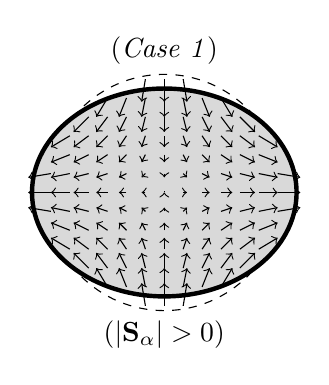
\begin{tikzpicture}[ultra thick,scale=0.6]
        \def\nRows{6}
        \def\nCols{6}
        \draw[dashed,thin] (0,0)circle(2.5);
        \draw[fill=gray!30] (0,0)ellipse(2.8 and 2.2);
        \foreach \x in {-\nRows,...,\nRows} {
            \foreach \y in {-\nCols,...,\nCols} {
                \pgfmathsetmacro\distance{veclen(\x*0.4, \y*0.4)};
                \pgfmathparse{\distance < 2.45 ? "blue" : "white"}
                \edef\colour{\pgfmathresult};
                \ifthenelse{\equal{\colour}{blue}}{                    
                    \draw[thin,->](\x*0.4,\y*0.4)--++(0.08*\x,-0.08*\y);
                }
            }
        }
        \node (txt) at (0,3){(\textit{Case 1})};
        \node (txt) at (0,-3){($|\textbf{S}_\alpha| > 0$)};
    \end{tikzpicture}
     \hfill
    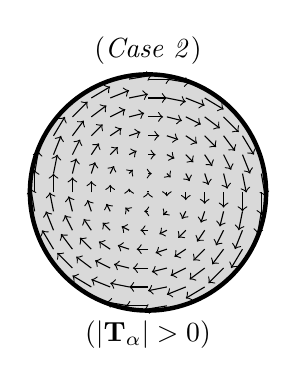
\begin{tikzpicture}[ultra thick,scale=0.6]
        \def\nRows{6}
        \def\nCols{6}
        \draw[fill=gray!30] (0,0)circle(2.5);
        \foreach \x in {-\nRows,...,\nRows} {
            \foreach \y in {-\nCols,...,\nCols} {
                \pgfmathsetmacro\distance{veclen(\x*0.4, \y*0.4)};
                \pgfmathparse{\distance < 2.5 ? "blue" : "white"}
                \edef\colour{\pgfmathresult};
                \ifthenelse{\equal{\colour}{blue}}{                    
                    \draw[thin,->](\x*0.4,\y*0.4)--++(0.08*\y,-0.08*\x);
                }
            }
        }
        \node (txt) at (0,3){(\textit{Case 2})};
        \node (txt) at (0,-3){($|\textbf{T}_\alpha| > 0$)};
    \end{tikzpicture}
    \hfill
    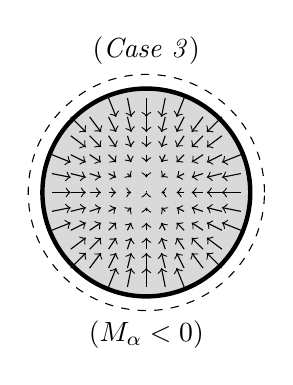
\begin{tikzpicture}[ultra thick,scale=0.6]
        \def\nRows{6}
        \def\nCols{6}
        \draw[dashed,thin] (0,0)circle(2.5);
        \draw[fill=gray!30] (0,0)circle(2.2);
        \foreach \x in {-\nRows,...,\nRows} {
            \foreach \y in {-\nCols,...,\nCols} {
                \pgfmathsetmacro\distance{veclen(\x*0.4, \y*0.4)};
                \pgfmathparse{\distance < 2.3 ? "blue" : "white"}
                \edef\colour{\pgfmathresult};
                \ifthenelse{\equal{\colour}{blue}}{                    
                    \draw[thin,->](\x*0.4,\y*0.4)--++(-0.08*\x,-0.08*\y);
                }
            }
        }
        \node (txt) at (0,3){(\textit{Case 3})};
        \node (txt) at (0,-3){($M_\alpha < 0$)};
    \end{tikzpicture}
    \hfill
    \caption{Graphical representation of the inner kinematics   of an arbitrary particle under three scenarios. 
        The arrows represent the velocity field inside the particle, $\textbf{w}_d^0$, with the corresponding value of the moment of momentum tensor indicated below. 
        The operator $|\ldots|$ refers to the norm of the tensors. 
        According to the inner velocity field:
        (\textit{Case 1}) The particle experiences a mean rate of deformation, resulting in non-zero stretching of momentum along the principal axis of deformation;
        (\textit{Case 2}) The particle is rotating, leading to a non-zero angular momentum vector in the direction of rotation;
        (\textit{Case 3}) The particle undergoes compression, resulting in a negative trace of the moment of momentum.
    }
    \label{eq:scheme}
\end{figure}

% \section{Conservation laws}



% \subsection{Inside the volume}

 


% Let us consider the specific case of the momentum balance, i.e. $q_\alpha = \textbf{p}_\alpha$.
% In this situation, \ref{eq:dt_q_alpha} reads
% \begin{equation}
%     \ddt  \textbf{p}_\alpha
%     = \intO{ \rho_d\textbf{g} }
%     + \intS{ 
%         \left[
%         f_d^0 (\textbf{u}_\Gamma^0-\textbf{u}_d^0)
%          + \bm{\sigma}_d^0%\cdot\textbf{n}_d  
%         %+ \mathbf{\Phi}_d^0 
%         \right] 
%         \cdot \textbf{n}_d },
% \end{equation}
% first term reads as $\intO{ \rho_d\textbf{g} }$ 
% The first term on the right-hand side represents the total weight acting on the particle $\alpha$, 
% the second term represents the total source of momentum due to phase transfer, and it is expressed as, $\intS{ \rho_d \textbf{u}_d^0 (\textbf{u}_\Gamma^0-\textbf{u}_d^0)\cdot\textbf{n}_d }$,
% and the last term $\intS{ \bm{\sigma}_d^0\cdot\textbf{n}_d }$, represents the resultant of the hydrodynamic forces acting on the surface of the particle.
% It is important to note that under this form, the exchange terms are expressed as integrals of dispersed phase fields denoted by the subscript $_d$.
% Nevertheless, depending on the nature of the dispersed phase, these fields may not always be defined.
% For rigid particles the stress within the particle $\bm{\sigma}_d^0$ is indeterminate \citep{guazzelli2011}.  
% Hence, our objective is to express these exchange terms, in terms of the continuous phase field quantities instead of the dispersed phase fields, i.e. in terms of $\mathbf{\Phi}_f^0$ and $\textbf{u}_f^0$ rather than $\mathbf{\Phi}_d^0$ and $\textbf{u}_d^0$. 

%\subsection{On the interfaces}
 

%For completeness, we exposed in \ref{ap:particles_eq} a clear derivation of the mass, momentum and total energy equations for a single particle.
%The derivation takes place using the same hypothesis as it is exposed in \ref{ap:hypothesis}.
%Especially, it is shown that the integration of the kinetic energy jump condition corresponds to the Lagrangian derivative of the particle surface, see \ref{eq:int_u_I2}.



\subsubsection{Zeroth-order conservation laws}

Using the local conservation, \ref{eq:dt_rho}, \ref{eq:dt_rhou_k} and \ref{eq:dt_rhoE_k} into the generic formulation \ref{eq:dt_q_alpha} yields directly the mass momentum and total energy conservation equation for a single particle, namely
\begin{align}
    \ddt m_\alpha
    &= 
    0,\\
    \ddt (m_\alpha \textbf{u}_\alpha)
    &= 
    m_\alpha\textbf{g}
    +  \intS{\bm{\sigma}_d^0 \cdot \textbf{n}_d},\\
    \ddt (m_\alpha E_\alpha)
    &= 
    m_\alpha \textbf{u}_\alpha \cdot \textbf{g}
    +\intS{\textbf{u}_d^0 \cdot \bm{\sigma}_d^0 \cdot  \textbf{n}_d} 
    - \intS{\textbf{q}_d^0 \cdot \textbf{n}_d}. 
\end{align}
As mentioned in \ref{sec:Lagrangian} we now need to derive the particle's surface equations to re-formulate the exchange terms on the right-hand side of these equations. 
It is done by integrating \ref{eq:surface_tension}, \ref{eq:dt_rhoI_uI3} and  \ref{eq:dt_rhoIe_I}  over the surface of the particle, which gives,  
\begin{align}
    \label{eq:int_u_I}
    \intS{\Jump{\bm{\sigma}_k^0} }
    &=
    \intS{\divI\bm\sigma^0_{\Gamma||}} = 0\\
    \label{eq:int_u_I2}
    \intS{\Jump{\textbf{u}_k^0 \cdot \bm{\sigma}_k^0}},
    % = \intS{\Jump{\textbf{w}_k^0 \cdot \bm{\sigma}_k^0}},
    &=
    -\intS{\gamma(\textbf{n}\cdot \textbf{u}_{\Gamma}^0)(\div \textbf{n})}
    = \gamma \ddt s_\alpha,\\
    \label{eq:int_q_I}
    \intS{\Jump{\textbf{q}_k^0}}
    &=
    0,
\end{align}
for the momentum, kinetic, and internal energy of the surface, respectively. 
The second equality of \ref{eq:int_u_I} is demonstrated using \ref{eq:gauss_surface}. 
The second equality of \ref{eq:int_u_I2} is derived noticing that $\intS{\gamma(\textbf{n}\cdot \textbf{u}_{\Gamma}^0)(\div \textbf{n})} = \intS{\divI (\gamma \textbf{u}_I^0)} $ using \ref{eq:gauss_surface} and then the last identity is obtained by using \ref{eq:reynolds_transport}. 
As witnessed by \ref{eq:int_u_I}, on a closed surface the surface tension plays no role in the momentum jump condition.
Additionally, according to \ref{eq:int_u_I2} the work of the surface tension force is equal to $\gamma$ times the rate of change of the area of a given particle. 

Using \ref{eq:int_u_I}, \ref{eq:int_u_I2} and \ref{eq:int_q_I} to reformulate the preceding equations, we easily derive the total mass, momentum, and energy equations for a single particle, 
\begin{align}
    \label{eq:dt_m_alpha}
    \ddt m_\alpha
    &= 
    0\\
    \label{eq:dt_p_alpha}
    \ddt (m_\alpha \textbf{u}_\alpha)
    &= 
    m_\alpha\textbf{g}
    +  \intS{\bm{\sigma}_f^0 \cdot \textbf{n}_d}\\
    \label{eq:dt_E_alpha_tot}
    \ddt (m_\alpha E_\alpha^\text{tot})
    &= 
    m_\alpha \textbf{u}_\alpha \cdot \textbf{g}
    +\textbf{u}_\alpha \cdot \intS{\bm{\sigma}_f^0 \cdot \textbf{n}_d}
    +\intS{\textbf{w}_f^0 \cdot \bm{\sigma}_f^0 \cdot  \textbf{n}_d} 
    - \intS{\textbf{q}_f^0 \cdot \textbf{n}_d}
\end{align}
where  $\intS{  \bm{\sigma}_f^0 \cdot \textbf{n}_d }$ is the resultant of the hydrodynamic forces of the continuous phase, $\intS{\textbf{w}_f^0 \cdot \bm{\sigma}_f^0 \cdot  \textbf{n}_d} $ is the resultant of the work of the continuous phase stresses with the surface velocity, and $\intS{ \textbf{q}_f^0 \cdot \textbf{n}_d }$ is the resultant of the surface heat flux. 
Note that the second term on the right-hand side of \ref{eq:dt_E_alpha_tot} is the work produced by the mean force and the translational motion of the droplets, while $\intS{\textbf{w}_f^0 \cdot \bm{\sigma}_f^0 \cdot  \textbf{n}_d}$ is the work produced by the local forces and local motion of the fluid at the surface of the particle.
Note that these equations do not explicitly account for inter-particle interactions. 
Nevertheless, the surface external stress flux $\bm{\sigma}_f^0$ contains inter-particle forces mediated through the carrier fluid such as lubrication forces and long-range inter-particle forces.

In the spirit of the energy decomposition exposed in the previous section (\ref{eq:dt_rhou_k2} and \ref{eq:dt_rhoe_k}) the total energy equation \ref{eq:dt_E_alpha_tot} can be split into three secondary equations. 
One for the center of mass kinetic energy $u_\alpha^2/2$, another for the particle internal kinetic energy $W_\alpha$, and a last one for the particle internal energy $e_\alpha$, which read
\begin{align}
    \label{eq:dt_u2_alpha}
    \frac{1}{2}\ddt (m_\alpha u_\alpha^2)
    &= 
    m_\alpha\textbf{u}_\alpha\cdot
    \textbf{g}
    + 
    \textbf{u}_\alpha\cdot
    \intS{\bm\sigma_f^0 \cdot \textbf{n}_d},\\
    \label{eq:dt_w2_alpha}
    \ddt (W_\alpha + \gamma s_\alpha)
    &= 
    - \intO{ \bm{\sigma}_d^0 : \grad\textbf{u}_d^0 }
    + \intS {\textbf{w}_f^0 \cdot \bm{\sigma}_f^0 \cdot \textbf{n}_d }
    \\
     \label{eq:dt_e_alpha}
    \ddt (m_\alpha e_\alpha )
    &= 
     \intO{ \bm{\sigma}_d^0 : \grad\textbf{u}_d^0  }
    -  \intS{\textbf{q}_f^0\cdot \textbf{n}_d } 
\end{align}
respectively. 
The first equation is obtained by taking the dot product of \ref{eq:dt_p_alpha} with $\textbf{u}_\alpha$. 
The third equation is directly obtained using the local conservation of $e_k^0$ (\ref{eq:dt_rhoe_k}) and setting $f_d^0 = e_d^0$ in \ref{eq:dt_q_alpha_tot}.
The last equation is obtained by subtracting the first and third equations from \ref{eq:dt_E_alpha_tot}. 
Note that under this form the surface energy is part of the total energy to be conserved, while it could also be treated as a source term using the first formulation of \ref{eq:int_u_I2}.
From this set of equation we can easily see that the rate of dissipation term $\intO{\bm{\sigma}_d^0 : \grad\textbf{u}_d^0}$ represents an energy sink in the equation of $W_\alpha$ while it is a source term in the internal energy equation. 
As it has been observed in the previous section, this term convert the energy of internal motion into molecular agitation. 
However, the interplay between the center of mass kinetic energy and the internal fluctuations is not obvious, indeed \ref{eq:dt_u2_alpha} shares no common term with the heat and internal kinetic energy equation.
We will see that the transfer between these scales is achieved through the fluid-phase pseudo-turbulent energy. 



\subsubsection{Higher-order conservation laws}


Injecting, $f_d^0 = \rho_d$ in the second-order moment equation (derived in \ref{ap:Moments_equations}) we obtain:
\begin{equation}
    \ddt {\textbf{M}_\alpha}=2\textbf{S}_\alpha, 
    \label{eq:dt_M_alpha}
\end{equation}
which is the second-order moment of mass conservation equation. 
From \ref{eq:dt_M_alpha} we deduce that the evolution of the distribution of mass of a particle is solely determined by the stretching of momentum $\textbf{S}_\alpha$. 
This implies that the angular momentum plays no role in the evolution of the second moment of mass. 
This is due to the symmetry of the tensor $\textbf{M}_\alpha$, which must be preserved after differentiation with respect to time.
Nevertheless, that does not mean that the particle angular velocity (noted $\bm\omega_\alpha$ here) has no role in the equation. 
As an example let us consider solid body motion, such that $\textbf{w}_d^0 = \bm\omega_\alpha \times \textbf{r}$, in that case we found, $2\textbf{S}_\alpha = \bm\omega_\alpha \times \textbf{M}_\alpha+ \textbf{M}_\alpha\times \bm\omega_\alpha $. 
Therefore, the angular velocity plays a significant role in the evolution of the second moment of mass equation. 
Additionally, if $\textbf{M}_\alpha$ is constant under change of reference frame, such as for spherical particles where we can write $\textbf{M}_\alpha= \frac{a^2 m_\alpha}{5} \bm\delta$, then $\textbf{S}_\alpha=0$ since $\ddt \textbf{M}_\alpha = 0$ in this situation.
This argument is not restricted to solid particles, thus it is also true for fluid particles with possible inner motion. 
Additionally, applying the trace operator on both sides of \ref{eq:dt_M_alpha}, yields the relation $\ddt {M_\alpha}=\frac{2}{3}\bm\delta : \textbf{S}_\alpha$.
We can state that $M_\alpha = \lambda^\alpha_1(t)+\lambda^\alpha_2(t)+\lambda^\alpha_3(t)$, with $\lambda_i^\alpha$ for $i=1,2,3$, the eigenvalues of $\textbf{M}_\alpha$, as it is a symmetric tensor and thus always diagonalizable.
For undeformable particles, it is evident that the eigenvalues are not functions of time, implying $\ddt M_\alpha = 0$.  
Consequently, $\bm\delta : \textbf{S}_\alpha$ possesses the notable property of being zero whenever the particle shape remains constant, regardless of the orientation.

Now that we have described the kinematics   of the particle shape, let us proceed to derive an equation for the dynamics of the particle shape, i.e. an equation for the moment of momentum. 
This equation is derived injecting $\textbf{Q}_\alpha = \textbf{P}_\alpha$ in \ref{eq:dt_Q_alpha_tot}, it reads, 
\begin{equation}
    \ddt {\textbf{P}_\alpha}
    - \intO{ \rho_d  \textbf{w}_d^0 \textbf{w}_d^0 }
    = 
    - \intO{\bm{\sigma}_d^0}
    - \intS{ 
        \gamma (\bm\delta - \textbf{nn})
    }
    + \intS{ \textbf{r}\bm{\sigma}_f^0\cdot \textbf{n}_d}.
    \label{eq:dt_P_alpha}
\end{equation}
On the left-hands side of \ref{eq:dt_P_alpha} we identify two inertial terms, i.e. the derivative of $\textbf{P}_\alpha$ and the internal velocity term $\intO{\rho_d\textbf{w}_d^0\textbf{w}_d^0 }$.
The inertia of the particle is then balanced by the terms on the right-hand side of the equation, namely: 
the integral of the particle internal stress $\intO{ \bm{\sigma}_d^0}$; 
the integral of the surface tension stress $\intS{ \gamma (\bm\delta- \textbf{nn}) }$; 
and the first moment of the hydrodynamic stress tensor, $\intS{\textbf{r}\bm\sigma_f^0\cdot \textbf{n}}$.
A discussion regarding the physical implications of this equation is provided below. 

The conservation equation of the angular momentum $\bm{\mu}_\alpha$ is obtained by taking the double contracted product of \ref{eq:dt_P_alpha} with $\bm\epsilon$, which directly gives
\begin{equation}
    \ddt\bm{\mu}_\alpha
    =  
    % \textbf{t}_\alpha.
    \intS{ \textbf{r} \times \bm{\sigma}_f^0\cdot \textbf{n}_d }
    \label{eq:dt_mu_alpha}
\end{equation}
Note that every term on the right-hand side of \ref{eq:dt_P_alpha} vanished due to their symmetric nature apart from the skew-symmetric part of the hydrodynamic stress, which is the hydrodynamic torque applied on the particle $\alpha$.
In particular, the surface tension terms do not appear in the angular momentum balance since $\bm\sigma_\Gamma^0 = \gamma (\bm\delta-\textbf{nn})$ is symmetric, which is consistent with the findings of \citet{hesla1993note}. 
As a consequence, the surface tension does not affect the angular momentum regardless of the particle's shape. 
In the literature, it is common to include the torque due to inter-particular interactions in the angular momentum balance, as is done in \citet{jackson1997locally} and \citet{zhang1997momentum}.
In our case note that $\bm{\sigma}_f^0$ contains short-range hydrodynamic interaction forces. 

Taking the double contracted product of \ref{eq:dt_P_alpha} with the tensor $\bm\delta$ and using \ref{eq:dt_M_alpha}, yields directly  
% \begin{equation}
%     \frac{1}{2}\ddt^2 {M_\alpha}
%     - \frac{1}{3}\intO{ \rho_d \textbf{w}_d^0 \cdot \textbf{w}_d^0}
%     = 
%     \intO{p_d^0} 
%     % - \frac{1}{3}\intS{p_f^0 \textbf{r}\cdot \textbf{n}}
%     - \frac{2}{3} \gamma s_\alpha
%     - \frac{1}{3}\intS{p_f^0 \textbf{r}\cdot \textbf{n}}
%     + \frac{1}{3}\intS{\textbf{r}\cdot\bm\tau_f^0\cdot \textbf{n}},
%     \label{eq:dt_D_alpha}
% \end{equation}
\begin{equation}
    \frac{3}{2}\frac{d^2 M_\alpha}{dt^2}
    - \intO{ \rho_d \textbf{w}_d^0 \cdot \textbf{w}_d^0}
    = 
    - \intO{\bm\sigma_d^0:\bm\delta} 
    % - \frac{1}{3}\intS{p_f^0 \textbf{r}\cdot \textbf{n}}
    - \gamma 2 \intS{}
    % - \frac{1}{3}\intS{p_f^0 \textbf{r}\cdot \textbf{n}}
    + \intS{\textbf{r}\cdot\bm\sigma_f^0\cdot \textbf{n}}.
    \label{eq:dt_D_alpha}
\end{equation}
\ref{eq:dt_D_alpha}, corresponds to the isotropic work balance over the volume and surface of the particle. 
According to \ref{eq:dt_D_alpha}, the rate of compression of a particle, denoted by the second derivative of $M_\alpha$ evolves according to : 
the internal inertial term, $\intO{\rho_d \textbf{w}_d^0 \cdot \textbf{w}_d^0 }$;
the particle internal pressure $\intO{\bm\sigma_d^0:\bm\delta}$; 
the surface energy $\gamma\intS{  }$; 
and the trace of the hydrodynamic first moment $\intS{\textbf{r}\cdot\bm\sigma_f^0\cdot \textbf{n}}$.
If one considers spherical particles composed of compressible fluid, \ref{eq:dt_D_alpha} transforms into the Rayleigh-Lamb-Plesset equation as demonstrated in the unpublished work of \citep{danielcours}. 
In the steady-state regime, this reduces to the Young-Laplace equation, as indicated by the presence of the first three terms on the right-hand side of \ref{eq:dt_D_alpha}. 

% \tb{
%     As an example we now consider the \textit{Rayleigh-Lamb-Plesset} equation for spherical bubbles with radius $a_\alpha(t)$. 
%     As the droplets remain spherical while keeping a constant mass the moment of momentum and inner velocity field can be expressed, 
%     \begin{align*}
%         M_\alpha
%         = \frac{m_\alpha}{5} a^2_\alpha(t),
%         && 
%         \textbf{w}_d^0
%         = \frac{d a_\alpha}{dt}\frac{\textbf{r}}{a_\alpha(t)},
%         \label{eq:expr1}
%     \end{align*}
%     where it is empathized that the radius $a_\alpha(t)$ is time-dependent. 
%     The stress inside the bubbles might be expressed as compressible Newtonian fluids with no resistance to shear such that 
%     \begin{equation}
%         \bm\sigma_d^0 
%         = 
%         - p_d^0 \bm\delta
%         - \lambda_d (\div \textbf{u}_d^0) \bm\delta
%         % + \mu_d \left[\grad \textbf{u}_d^0 + (\grad \textbf{u}_d^0)^\dagger\right]
%         = 
%         - p_d^0 \bm\delta
%         - \frac{3 \lambda_d}{a_\alpha} \frac{d a_\alpha}{dt}  \bm\delta
%         % + \mu_d \left[\grad \textbf{u}_d^0 + (\grad \textbf{u}_d^0)^\dagger\right]
%         \label{eq:StressBubbles}
%     \end{equation}
%     where $\lambda_d^0$ is the volume viscosity of the dispersed phase. 
%     Assuming incompressible Newtonian fluid for the continuous phase and injecting the expressions \ref{eq:StressBubbles} and \ref{eq:expr1} into \ref{eq:dt_D_alpha} yields, 
%     \begin{equation}
%         \frac{1}{5} \rho_d^0 a_\alpha \frac{d^2 a_\alpha}{dt^2} 
%         - 
%         \frac{1}{a_\alpha} \frac{d a_\alpha}{dt} 
%         \left(
%             3 \lambda_d
%             + 2 \mu_f 
%         \right)
%         = 
%         +  \frac{1}{v_\alpha}\intO{p_d^0}
%         -  \frac{1}{s_\alpha}\intS{p_f^0}
%         - \gamma  \frac{2}{a}
%     \end{equation}
%     By expressing the fluid pressure on the surface in terms of the far field pressure (see daniel) one obtain the \textit{Rayleigh-Lamb-Plesset} equation. 
%     In the static regime we recover laplace eq
% }

Taking the symmetric part of \ref{eq:dt_P_alpha}, and making use of \ref{eq:dt_M_alpha}, yields a dynamical balance equation for $\textbf{M}_\alpha$, namely
% \begin{multline}    
%     \frac{1}{2}\ddt^2{\textbf{M}_\alpha^\text{dev}}
%     - \intO{\left(
%         \rho_d\textbf{w}_d^0 \textbf{w}_d^0
%         - \rho_d\frac{1}{3}(\textbf{w}_d^0 \cdot \textbf{w}_d^0)\bm\delta\right)}
%     =  
%         - \mu_d \intO{\textbf{e}_d^0}
%         - \intS{\gamma\left(\frac{1}{3}\bm\delta-\textbf{nn}\right)}\\
%         + \frac{1}{2}\intS{\left(\textbf{r}\bm\sigma_f^0+ \bm\sigma_f^0\textbf{r} - \frac{2}{3}(\bm\sigma_f^0\cdot \textbf{r})\bm\delta\right)\cdot \textbf{n}}
%     \label{eq:dt_S_alpha}
% \end{multline}
\begin{equation}    
    \frac{1}{2}\frac{d^2 \textbf{M}_\alpha}{dt^2}
    - \intO{ \rho_d  \textbf{w}_d^0 \textbf{w}_d^0 }
    = 
    - \intO{\bm{\sigma}_d^0}
    - \intS{\gamma (\bm\delta - \textbf{nn})}
    + \frac{1}{2}\intS{(\textbf{r}\bm{\sigma}_f^0+\bm{\sigma}_f^0 \textbf{r})\cdot \textbf{n}_d}.
    \label{eq:dt_S_alpha}
\end{equation}
On the left-hand side of \ref{eq:dt_S_alpha}, we recover the symmetric part of the inertial contributions. 
In opposition to \ref{eq:dt_P_alpha} we could substitute the term $\ddt (\textbf{P}_\alpha+\textbf{P}_\alpha^\dagger)$ initially present in the equation by $\ddt^2 \textbf{M}_\alpha$ using \ref{eq:dt_M_alpha}. 
Consequently, \ref{eq:dt_S_alpha} is a second-order partial differential equation for the droplet mean deformation. 
In our case, only the external contribution $\intS{\textbf{r}\bm\sigma_f^0\cdot \textbf{n}}$ is responsible for the generation of angular momentum, see \ref{eq:dt_mu_alpha}.
Taking the symmetric part of this tensor ultimately removes this contribution. 
Thus, on the right-hand side of \ref{eq:dt_S_alpha}, we identify the terms responsible for the droplet deformation exclusively.
Therefore, \ref{eq:dt_S_alpha} must be interpreted as an equation for the shape of the particle, represented by the tensor $\textbf{M}_\alpha$.
One might immediately recognize that \ref{eq:dt_S_alpha} is in fact an extension of \citet{batchelor1970stress}'s famous result, 
\begin{equation}
    \intO{\bm{\sigma}_d^0}
    + \intS{\gamma(\bm\delta - \textbf{nn})}
    = \frac{1}{2}\intS{(\textbf{r}\bm\sigma_f^0+\bm\sigma_f^0\textbf{r})\cdot \textbf{n}},
    \label{eq:Batchelor}
\end{equation}
but with the consideration of the inertia of the particle.
\ref{eq:Batchelor} is particularly useful to compute the unknown internal stress within solid particles (for which $\gamma = 0$), in terms of surface integral, i.e. the stresslet $\intS{(\textbf{r}\bm\sigma_d^0+ \bm\sigma_d^0\textbf{r})\cdot \textbf{n}}$.
This relation is the main tool used to express the bulk stress of a suspension.
It eventually leads to the computation of the famous Einstein equivalent viscosity, upon having a closed expression for the average of $\intS{(\textbf{r}\bm\sigma_d^0+ \bm\sigma_d^0\textbf{r})\cdot \textbf{n}}$ \citep{guazzelli2011}. 
In the inertial case, due to the limited degree of freedom of solid particles, the tensors $\textbf{M}_\alpha$ and the inner velocity field $\textbf{w}_d^0$ are fully determined by \ref{eq:dt_M_alpha} and \ref{eq:dt_mu_alpha}, indicating that $\textbf{M}_\alpha$ and $\textbf{w}_d^0$ can be used in \ref{eq:dt_S_alpha} not as unknowns but as source terms. 
Consequently, for solid particles, \ref{eq:dt_S_alpha} must be interpreted as a generalized equation for the undefined stress $\bm\sigma_d^0$ integrated on the volume of the particles.
Whether it is solid or fluid particles \ref{eq:dt_S_alpha} becomes particularly relevant for expressing the averaged stress within an inertial suspension in terms of Lagrangian properties, as discussed in the next chapter. 

It is now clear that if the surface tension forces play no role in the linear and angular momentum equation, however, it impacts the moment of momentum $\textbf{P}_\alpha$ or more specifically its symmetric part $\textbf{S}_\alpha$.
Thus, the surface tension force impacts the hydrodynamic behavior of a particle solely through its action on $\textbf{S}_\alpha$, which is related to the shape of a particle represented by $\textbf{M}_\alpha$, through \ref{eq:dt_M_alpha}.
In \ref{ap:Moments_equations} we show how to derive the higher-order moment of momentum equations, which can also be viewed as formulas for the higher moments of the internal particle stress distribution. 
It is interesting to mention that in a recent study of \citet{dolata2021faxen} and \citet{zhou2020lamb} they make use of the first two moments of momentum equations hidden into another but equivalent form, valid in the Stokes flow regime. 



\section{The two-fluid model}
\label{ap:two-fluid_model}

% \subsubsection{Volume equation}
Using the generic formulation \ref{eq:avg_dt_chi_f} and the local expression of the mass, momentum and total energy equation, i.e. : \ref{eq:dt_rho},\ref{eq:dt_rhou_k} and \ref{eq:dt_rhoE_k} we easily find the averaged form of the mass, momentum and total energy equation.
They read, 
\begin{align}
    \label{eq:dt_avg_rho}
    \pddt (\phi_k \rho_k)  
    + \div (
        \phi_k \rho_k\textbf{u}_k
    )
    &= 
    0\\
    \label{eq:dt_avg_rhou_k}
    \pddt (\phi_k \rho_k\textbf{u}_k)  
    + \div (
        \phi_k \rho_k\textbf{u}_k\textbf{u}_k
        + \bm{\sigma}_k^\text{eq}
    )
    &= 
    \phi_k \rho_k \textbf{g} 
    +  \avg{\delta_I \bm{\sigma}_k^0 \cdot \textbf{n}_k}\\
    \label{eq:dt_avg_rhoE_k}
    \pddt (\phi_k\rho_kE_k)  
    + \div (
        \phi_k\rho_kE_k\textbf{u}_k
        + \bm{q}_k^\text{eq}
        + \textbf{u}_k \cdot \bm{\sigma}_k^\text{eq}
        % - \textbf{u}_k^0 \cdot \bm{\sigma}_k^0 
        % + \textbf{q}_k^0
        )
    &= 
    \phi_k \rho_k\textbf{u}_k \cdot \textbf{g} 
    + \avg{\delta_I (\textbf{u}_k^0 \cdot \bm{\sigma}_k^0 - \textbf{q}_k^0)\cdot \textbf{n}_k}
\end{align} 
with the equivalent stress and heat flux defined as, 
\begin{align*}
    &\bm{\sigma}_k^\text{eq}
    = 
     \rho_k\avg{\chi_k \textbf{u}_k'\textbf{u}_k'}
      - \phi_k \bm{\sigma}_k,%- n_p \textbf{M}_p
    &\textbf{q}_k^\text{eq}
    =\textbf{q}_k^\text{e} +\textbf{q}_k^\text{k},  \\
    &\textbf{q}_k^\text{e}
    = \rho_k \avg{\chi_k\textbf{u}_k' e_k'} 
    + \phi_k\textbf{q}_k,
    &\textbf{q}_k^\text{k}
    = \rho_k \avg{\chi_k \textbf{u}_k' k_k} 
    - \avg{\chi_k \textbf{u}_k' \cdot \bm{\sigma}_k^0}.
\end{align*}
% The main differences between these equations and their microscale counterpart, is that : (1) we have introduced a pre factor $\phi_k$ in front of most of the terms
% (2) an additional stress is present, that is the covariance between the quantity to be conserved and the velocity. 
% (3) A new source term appear on the RHS accounting for the exchange across the phases. 

The terms $\avg{\chi_k \textbf{u}_k'\textbf{u}_k'}$ will be referred as the Reynolds stress or pseudo turbulent stress. 
It has a fundamental importance in the multiphase flow problem and as we see now its trace is related to the mean kinetic energy. 
Indeed, the phase averaged total energy can be further decompose into three energy components, that is,  
\begin{align}
    E_k = e_k + k_k + u_k^2/2
    \label{eq:E_def}
\end{align}
where $k_k$ is the pseudo-turbulent kinetic energy defined as, $\phi_k k_k = \frac{1}{2}\avg{\chi_k \textbf{u}_k'\cdot \textbf{u}_k'}$. 
Each of the components of the total energy represent the averaged agitation at different scales. 
From molecular agitation which quantified by $e_k$, to the macroscopic scale agitation or kinematic energy $u_k^2$, and in between we find the pseudo turbulent energy $k_k$ which represents the local scale velocity fluctuation. 
To fully describe the averaged total energy one must add at least a supplementary equation either for $k_k$ or $e_k$ assuming \ref{eq:dt_avg_rhoE_k} is solved. 
Using \ref{eq:dt_avg_rhou_k} dotted with $\textbf{u}_k$ yields an equation for the mean kinetic energy. 
Averaging \ref{eq:dt_rhoe_k} yields un equation for $e_k$.  
Then, subtracting these two equations to \ref{eq:dt_avg_rhoE_k} gives us an equation for $k_p$. 
The kinetic energy, pseudo turbulent and internal averaged equations read as, 
\begin{align}
    \label{eq:dt_avg_uk2}
    &\pddt (\phi_k \rho_ku_k^2/2)  
    + \div (
        \phi_k \rho_k\textbf{u}_ku_k^2/2
        + \textbf{u}_k \cdot \bm{\sigma}_k^\text{eq}
    )
    = 
    \bm{\sigma}_k^\text{eq} : \grad \textbf{u}_k
    + \phi_k \rho_k \textbf{u}_k\cdot \textbf{g} 
    +  \textbf{u}_k\cdot \avg{\delta_I \bm{\sigma}_k^0 \cdot \textbf{n}_k},\\
    \label{eq:dt_avg_kk}
    &\pddt (\phi_k\rho_kk_k)  
    + \div (
        \phi_k\rho_kk_k\textbf{u}_k
        + \textbf{q}_k^\text{k} 
        )
    = 
    - \avg{\chi_k\bm{\sigma}_k^0 : \grad \textbf{u}_k^0}
    - \bm{\sigma}_k^\text{eq} : \grad \textbf{u}_k
    + \avg{\delta_I \textbf{u}_k' \cdot \bm{\sigma}_k^0 \cdot \textbf{n}_k},\\
    \label{eq:dt_avg_ek}
    &\pddt (\phi_k\rho_ke_k)  
    + \div (
        \phi_k \rho_ke_k\textbf{u}_k
        +
        \textbf{q}_k^\text{e} 
        )
    = 
    \avg{\chi_k\bm{\sigma}_k^0 : \grad \textbf{u}_k^0}
    - \avg{\delta_I \textbf{q}_k^0 \cdot \textbf{n}_k},
\end{align}
respectively. 
This derivation is in agreement with \citet{morel2015mathematical}. 
Under this form the energy transfer across scale is clear. 
Indeed, the term $\bm{\sigma}_k^\text{eq} : \grad \textbf{u}_k$ act as a sink term in \ref{eq:dt_avg_uk2} and a source term in \ref{eq:dt_avg_kk}, while the averaged diffusive terms $\avg{\chi_k\bm{\sigma}_k^0 : \grad \textbf{u}_k^0}$ is a sink in \ref{eq:dt_avg_kk} and a source in \ref{eq:dt_avg_ek}. 
To determine the total energy only two of the four energy equations must be solved. 
In practice, it is useful to solve one equation for $k_k$ since it is useful for the Reynolds stress modeling since $\avg{\chi_k \textbf{u}_k^0 \textbf{u}_k^0}: \bm\delta = 2 k_k$, and another for $e_k$ since $u_k^2$ is already determined by the momentum equation. 

% \subsubsection{Averaged surface equations}
The volume averaged equations must be completed by an averaged surface transport equation.  
For this purpose we multiply \ref{eq:surface_tension}, \ref{eq:dt_rhoIe_I} and \ref{eq:dt_rhoI_uI3} by $\delta_I$ and apply the average operator.
By considering the topological equations we obtain the  momentum, kinetic and internal energy averaged surface equations, namely
\begin{align}
    \label{eq:dt_avg_uI}
    \avg{\delta_I \Jump{\bm{\sigma}^0_k}}
    &= -\gamma \div \avg{\delta_I (\bm\delta - \textbf{nn})},\\
    \label{eq:dt_avg_gamma}
    \avg{\delta_I \Jump{\textbf{u}_k^0 \cdot \bm{\sigma}^0_k}}
    &= - \gamma \left[
        \pddt \avg{\delta_I}
        +  \div \avg{\delta_I (\textbf{u}_{I}^0 \cdot \textbf{n})\textbf{n} },
    \right]\\
    \avg{\delta_I \Jump{\textbf{q}^0_k}}
    &= 0
\end{align}
respectively. 
The first equation represents the contribution of the surface tension stresses to the bulk momentum equation.
The second equation represents the amount of energy stored as surface deformation.
And the last equation witnesses of the continuity of heat flux through the interface. 



\section{The bulk stress in dispersed multiphase flow}
\label{sec:symetric_stress}


One of the major questions in suspension dynamic raised by several authors, is the evaluation of the bulk stress or equivalent stress tensor of a suspension, see \citep{batchelor1970stress, prosperetti2006stress,zhang1997momentum,nadim1996concise} and more recently \citet{dolata2020heterogeneous}. 
Specifically, we seek to express the bulk stress in the suspension in terms of particle-averaged quantities. 
Only then it is possible to derive closures for the stress. 
Therefore, in this subsection we derive an expression for the bulk stress of an emulsion in terms of the Lagrangian particle quantities derived in the two previous sections. 
For the sake of generality in this section we consider that the flow is subjected to an arbitrary body force $\textbf{b}$. 

\subsection{The bulk stress formulation}

Before proceeding further, it is useful to clarify what we mean exactly by the \textit{bulk stress}.
The \textit{bulk stress} tensor is the force per unit of surface applied on the fluid and on the particles phases, having the form $\div \bm{\sigma}^\text{eq}_m$, which added to the total external force, balances exactly the material derivative of the mixture momentum, namely: $\pddt (\rho \textbf{u}_m) + \div (\rho \textbf{u}_m\textbf{u}_m)$. 
This definition of the bulk stress implies that the external body force term $\textbf{b}$ cannot be decomposed into a vector plus a divergence of a tensor, in which case the latter would just contribute to $\bm{\sigma}^\text{eq}$.
Thus, in this definition $\textbf{b}$ must be reformulated since $\textbf{b} = \phi_f \textbf{b}_f+\phi_d \textbf{b}_d$ and that the term $\phi_d \textbf{b}_d$ can be decomposed into a Taylor series according to \ref{eq:f_exp}. 
Therefore, the momentum equation is obtained by setting $\rho \textbf{g} = \textbf{b}$ in \ref{eq:dt_avg_rhou} and by reformulating the body force term accordingly we obtain,
\begin{align}
    \label{eq:momentum_bulk}
    \pddt (\rho^0 (\textbf{u}_m)_i)
    + \partial_j  [\rho (\textbf{u}_m \textbf{u}_m)_{ij}
    + (\bm\sigma_{m}^\text{eq})_{ij}]
    &= \left[\phi_f \textbf{b}_f + \pOavg{\textbf{b}}\right]_i
    % \epsilon_{ijk} \sigma_{jk}
    % &= 0 
    % \label{eq:angular_momentum_bulk}
\end{align}
% Indeed, in the averaged angular momentum equation we have assumed that no-body torque exist at the local scale making the skew-symmetric part of $\sigma_{jk}^0$ equal to $0$ \citet{leal2007advanced}. 
% Taking the average of the bulk momentum and angular momentum equation gives directly, 
Where we have defined the effective stress of the suspension as,
\begin{multline}
    \bm{\sigma}_m^\text{ed}
    = 
    \avg{\rho^0\textbf{u}_m'\textbf{u}'_m}
    + \phi_fp_f\bm\delta
    - 2\mu_f\textbf{e}
    - \phi_d(\bm{\sigma}_d - 2\mu_f \textbf{e}_d)
    - \phi_\Gamma \bm{\sigma}_\Gamma\\
    + \pOavg{\textbf{r}\textbf{b}_d^0}
    -\frac{1}{2} \div \pOavg{\textbf{rr}\textbf{b}_d^0} + \ldots
    \label{eq:sigma_bulk}
\end{multline}
% where we have used the relation 
The first term corresponds to the Reynolds stress, and the second third and fourth terms are obtained by noticing that 
$
    \phi_f \bm\sigma_f
    = -\phi_f p_f \bm\delta
    + 2\mu_f \textbf{e}
    - 2 \mu_f \phi_d \textbf{e}_d 
$
where $\phi_f p_f$ is the mean fluid pressure and $\textbf{e} = \grad \textbf{u} + ^\dagger(\grad \textbf{u})$ the averaged strain rate of the suspension. 
% The last two terms of \ref{eq:sigma_bulk} have been obtained by expanding the body force term $\phi_d \textbf{b}_d$ originally present on the right-hand side of \ref{eq:momentum_bulk} in a Taylor expansion according to \ref{eq:f_exp}. 
Additionally, we considered that the local angular momentum balance follows  $\epsilon_{ijk} \sigma_{jk}^0 = 0$. 
Due to the linearity of the ensemble average operator we deduce that the averaged stress also respects $\epsilon_{ijk} \sigma_{jk}$.
The interface stress also follows this condition since $\bm\sigma_I^0 = \gamma (\bm\delta - \textbf{nn})$ which is by definition symmetric.  
Thus, we can already conclude that the first five terms on the right-hand side of \ref{eq:sigma_bulk} are by definition symmetric since they are just averaged quantities of tensors which are by definition symmetric. 
Consequently, the only possible skew-symmetric contribution to the suspension stress must arise from the last two terms on the right-hand side of \ref{eq:sigma_bulk}.  
The discussion regarding the symmetry of $\bm\sigma^{eq}_m$ will be addressed in more detail at the end of this section. 

% The first moment contribution to the skew symmetric part is given by 
% \begin{equation}
%     \pOavg{\textbf{r}\textbf{b}_d^0 - \textbf{b}_d^0 \textbf{r}}. 
%     \label{eq:body_torque}
% \end{equation}
% This term corresponds to the averaged torque generated by the body force field $\textbf{b}^0$ on the particles. 
% Thus, all body force fields generating body torque will induce self toque in the suspension. 

% For the higher moment of body force the reasoning is slightly different.
% We use a methodology similar to \citep{lhuillier1992volume,lhuillier1996contribution} to re express the second and higher moment of the body force.  
% For convenience let us note 
% \begin{equation}
%     B_{ijk}
%     = \pOavg{\textbf{rr}\textbf{b}_d^0} - \frac{1}{3}\div \pOavg{\textbf{rrr}\textbf{b}_d^0} + \ldots
% \end{equation}
% % which represent the second plus the divergence of the higher order moment of the body forces. 
% Since this tensor is the sum of the second plus the higher moment it is not symmetric on any index. 

% We recall that the carrier fluid is a Newtonian fluid, therefore we may express the fluid phase stress as, 
Let us now present the bulk stress formulation in the \textit{hybrid} form, meaning in terms of particle-average quantities.  
The divergence of the dispersed phase stresses present in \ref{eq:momentum_bulk} through \ref{eq:sigma_bulk} may be expressed using \ref{eq:f_exp}, it gives
\begin{align}
    \label{eq:exp_e2}
    \partial_k (\phi_d \textbf{e}_d)_{ik} 
    &=  \partial_k\pSavg{ (\textbf e_d^0)_{ik} }
        -\frac{1}{2} \partial_k\partial_j \pSavg{ r_j (\textbf e_d^0)_{ik} +r_k (\textbf e_d^0)_{ij} }
        + \ldots  \\
    \label{eq:exp_sigma22}
    \partial_k (\phi_d \bm\sigma_d)_{ik}
    &=  \partial_k\pOavg{ (\bm\sigma_d^0)_{ik}}
    -\frac{1}{2} \partial_k\partial_j
    \pOavg{ r_j(\bm\sigma^0_d)_{ik} + r_k(\bm\sigma^0_d)_{ij}}
    + \ldots  \\
    \label{eq:exp_sigmaI2}
    \partial_k (\phi_\Gamma \bm\sigma_I)_{ik} 
    &=  \partial_k\pSavg{ (\bm\sigma_I^0)_{ik} }
        -\frac{1}{2} \partial_k\partial_j \pSavg{ r_j (\bm\sigma_I^0)_{ik} +r_k (\bm\sigma_I^0)_{ij} }
        + \ldots  
\end{align}
Note that we reformulated the second terms on the right-hand side of \ref{eq:exp_e2},\ref{eq:exp_sigma22} and \ref{eq:exp_sigmaI2} by retaining only their symmetric part since these terms must remain symmetric in the index $k$,$j$ due to the double contraction with the operator $\partial_k\partial_j$. 
Now we can use the first moment of momentum conservation \eqref{eq:dt_S_alpha} and the second moment of momentum equation (derived in \ref{ap:Moments_equations}, see \eqref{eq:second_momoent_of_momentum}) to reformulate the particle internal stresses, this yields,  
\begin{multline}
    \intS{ (\bm{\sigma}_\Gamma^0)_{ik}}
    +\intO{ (\bm{\sigma}_d^0)_{ik}}
    = 
    \intO{ \rho_d 
    (\textbf{w}_d^0\textbf{w}_d^0  )_{ik}
    }
    -\frac{1}{2}\left(\frac{d^2 \textbf{M}_\alpha}{dt^2} \right)_{ik}\\
    +\frac{1}{2}\intO{ \left[
        (\textbf{b}_d^0)_i
        r_k 
        + (\textbf{b}_d^0)_k
        r_i
    \right]}
    +
    \frac{1}{2}\intS{ \left[
        (\bm{\sigma}_1^0 \cdot \textbf{n}_d)_i r_k
        + (\bm{\sigma}_1^0 \cdot \textbf{n}_d)_k r_i
    \right]
    }
    \label{eq:dt_P1_alpha_bis}
\end{multline}
\begin{multline}
    \intO{ r_{j}(\bm{\sigma}^0_d)_{ik}+r_{k}(\bm{\sigma}^0_d)_{ji}}
    +\intS{ r_{j}(\bm{\sigma}^0_I)_{ik}+r_{k}(\bm{\sigma}_\Gamma^0)_{ji}}
    = 
    - \ddt\intO{ \rho_d (\textbf{u}_d^0)_i r_j r_k }
    \\
    + \intO{ \left[
        \rho_d (\textbf{u}^0_d\textbf{r}\textbf{w}_d^0)_{ijk} + \rho_d (\textbf{u}^0_d\textbf{r}\textbf{w}_d^0)_{kji}
    \right]}
    +\intS{  r_{k}r_{j} (\bm{\sigma}_1^0\cdot\textbf{n}_d)_i }
    + \intO{ r_{k}r_{j}  \rho_d (\textbf{b}_d^0)_i } 
    \label{eq:dt_P2_alpha_bis}
\end{multline}
By using an arbitrary order of moment of momentum equation (derived in \ref{ap:Moments_equations}) one can substitute any volume integral of the particle stress appearing in the expansion \ref{eq:exp_sigma22} into particles' kinematic properties plus the hydrodynamic moment of the fluid phase. 
Substituting \ref{eq:dt_P2_alpha_bis} and \ref{eq:dt_P1_alpha_bis} into \ref{eq:sigma_bulk} yields, 
\begin{multline}
    (\bm{\sigma}^\text{eq}_m)_{ik}
    = 
    \underbrace{
        % \left[
        \phi_f p_f 
        % + \frac{1}{3}\pOavg{\textbf{r}\cdot\bm{\sigma}_f^0 \cdot \textbf{n}_d} 
    % \right]
    \delta_{ik}
    - \mu_f e_{ik} 
    }_\text{Newtonian contribution}
    + \underbrace{\avg{\rho^0 \textbf{u}'_m\textbf{u}'_m}_{ik}}_\text{Bulk Reynolds stress}
    % + \mu_f \phi_2 e_{2,ik}. 
    + \underbrace{\epsilon_{ikj} \frac{1}{2}\pSavg{ (\textbf{b}_d^0 \times \textbf{r})_j}}_\text{Particles body torque}\\
    - \frac{1}{2}\underbrace{\pSavg{\left[
        (\bm{\sigma}_f^0 \cdot \textbf{n}_d)_kr_i  
        + (\bm{\sigma}_f^0 \cdot \textbf{n}_d)_i r_k
        % - \frac{2}{3}(\textbf{r}\cdot\bm{\sigma}_f^0 \cdot \textbf{n}_d)\delta_{ik}
    \right]}
    + 2 \mu_f \pOavg{(\textbf{e}_d^0)_{ik}}}_\text{Averaged Stresslet}\\
    - \underbrace{\pOavg{ \rho_d (\textbf{w}_d^0\textbf{w}_d^0  )_{ik}}
    + \pavg{\frac{d^2 \textbf{M}_{ik}}{dt^2}  }}_\text{particles inertia}
    + \underbrace{\frac{1}{2} (\div\bm{\Sigma})_{ik}}_\text{Inhomogeneous stresses}
    \label{eq:stress_bulk_explicit}
\end{multline}
with,
\begin{multline}
    \bm{\Sigma}
    = 
    - \pavg{\ddt\intO{ \rho_d (\textbf{u}_d^0)_i r_j r_k }}
    + \pOavg{ 
        \rho_d \left[
        (\textbf{u}^0_d\textbf{r}\textbf{w}_d^0)_{ijk} +  (\textbf{u}^0_d\textbf{r}\textbf{w}_d^0)_{kji}
    \right]
    }\\
    +\pSavg{  (\bm{\sigma}_f^0 \cdot \textbf{n}_d)_i r_{j}  r_{k}  }
    - 2 \mu_f \pOavg{[( \textbf{e}_d^0 \textbf{r})_{ikj}
    + ( \textbf{e}_d^0 \textbf{r})_{ijk}]} + \div[\ldots]
    \label{eq:Sigma_inhomo}
\end{multline}
We can note that the body force terms present in \ref{eq:sigma_bulk} and \ref{eq:dt_P2_alpha_bis} canceled each other in \ref{eq:Sigma_inhomo}. 
Under this form the different contributions to the suspension stress are explicit. 
The first contribution is the averaged continuous phase Newtonian stress. 
The second term is the  contribution from the total phase fluctuation to the suspension stress, including the particle internal fluctuation. 
The third term is the skew-symmetric part of the first moment of the body forces, in this study $\textbf{b}^0 = \rho^0 \textbf{g}$ thus this term vanishes for any kind of particles. 
The symmetric part of the hydrodynamic stresses together with the particle's internal shear rate form what is called: the Stresslet \citep{pozrikidis1992boundary}. 
Especially, we see in the next section that this term is related to the Einstein equivalent viscosity (see \ref{eq:fluid_phase_stress}). 
The first two terms on the third line of \ref{eq:stress_bulk_explicit} are the particle inertia contribution to the suspension stresses. 
This includes the second-order derivative of the particle shape represented by $\textbf{M}_\alpha$ and the internal particle motions. 
As discussed in the previous section this term is solely related to the inertia induced by change of orientation or deformation of the particles. 
Finally, the last term of the expression represents the contribution to the stress from all the higher moments related to the particles, it includes the moments related to the internal velocity or external hydrodynamic forces.  
Notice that since this term appears under the divergence operator it is non-zero only for Inhomogeneous suspension, therefore we call it the \textit{Inhomogeneous stresses}. 
The formulation of the bulk stress given by \ref{eq:stress_bulk_explicit} is formally equivalent to equation (8) and (12) of \citet{lhuillier1996contribution} and equation (8.2) of \citet{zhang1997momentum}.
The equivalence with \citet{zhang1997momentum} is not obvious as they use different decompositions for most of the terms. 
Although the relation \ref{eq:stress_bulk_explicit} is not new, the derivation presented here is original since the physical significance of all terms is explicit because it is derived in terms of particle-averaged quantities.

    
\subsection{Additional simplifications}

The averaged rate of strain, \textbf{e}, present in \ref{eq:stress_bulk_explicit} involves the averaged bulk velocity \textbf{u}. 
However, the momentum equation's purpose is to be solved for the Favre averaged velocity fields $\textbf{u}_m$. 
This means that two velocity fields are present in this equation meaning that a supplementary equation is needed to recover $\textbf{u}$ from $\textbf{u}_m$ and inversely. 
This inconsistency is easily fixed by noticing that, $\rho \textbf{u} = \sum_k \rho_k \phi_k \textbf{u}_k$, which implies that, 
\begin{equation}
    \textbf{u}=\rho \textbf{u}_m\sum_k \frac{1}{\rho_k \phi_k}
\end{equation}
Thus, we can recover the velocity field \textbf{u} needed in the expression of \textbf{e} through $\textbf{u}_m$ and the volume fractions. 

The only term in \ref{eq:stress_bulk_explicit} that is not expressed in terms of particle averaged quantities is the \textit{Reynolds stress} tensor, $\avg{\rho^0 \textbf{u}'_m\textbf{u}'_m}$. 
Indeed, the local field $\textbf{u}_m' = \textbf{u}^0 - \textbf{u}_m$ involves the local velocity fields within the particle.
From an experimental point of view, this quantity is difficult if not impossible to quantify.  
Therefore, it is interesting to reformulate this \textit{bulk Reynolds stress} in terms of continuous fluid phase averaged Reynolds stress and a stress related to particle averaged properties. 
This is easily done by noticing that, 
\begin{equation*}
    \avg{\rho^0 \textbf{u}'_m\textbf{u}'_m}
    = 
    \avg{\chi_f \rho_f \textbf{u}_f'\textbf{u}_f'}
    + \phi_f \rho_f \textbf{u}_f\textbf{u}_f
    - \rho \textbf{u}_m\textbf{u}_m
    + \avg{\chi_d \rho_d \textbf{u}_d^0\textbf{u}_d^0}
    \label{eq:u_mu_m}
\end{equation*}
We can notice that $\avg{\chi_f \rho_f \textbf{u}_f'\textbf{u}_f'}$ is the fluid phase Reynolds stress introduced in \ref{eq:dt_avg_rhou_k}. 
Regarding the last term of \ref{eq:u_mu_m} it can be reformulated as, 
\begin{equation*}
    \avg{\chi_d \rho_d \textbf{u}_d^0\textbf{u}_d^0}
    = 
    \pavg{ m_\alpha \textbf{u}_\alpha' \textbf{u}_\alpha' }
    + n_p m_p \textbf{u}_p\textbf{u}_p
    + \pOavg{\rho_d \textbf{w}_d^0 \textbf{w}_d^0}
    - \div [\ldots]
\end{equation*}
where we neglected the higher moments terms. 
Consequently, in \ref{eq:stress_bulk_explicit}, one can use the relation 
\begin{equation*}
    \avg{\rho^0 \textbf{u}'_m\textbf{u}'_m}
    - \pOavg{\rho_d \textbf{w}_d^0 \textbf{w}_d^0}
    \approx 
    \avg{\chi_f \rho_f \textbf{u}_f'\textbf{u}_f'}
    + \pavg{ m_\alpha \textbf{u}_\alpha'\textbf{u}_\alpha'}
    + \phi_f \rho_f \textbf{u}_f\textbf{u}_f
    + n_p m_p \textbf{u}_p\textbf{u}_p
    - \rho \textbf{u}_m\textbf{u}_m
\end{equation*}
to simplify the formulas. 
Using this formulation in \ref{eq:stress_bulk_explicit} one notices that the only quantity needed to express the bulk stress is the particle phase averaged quantities and $\textbf{u}_m$. 

\subsection{The symmetry of the bulk stress}

We now discuss the symmetry properties of $\bm\sigma^\text{eq}_m$ as it has been a subject of controversy over the past 20 years.
\citet{prosperetti2006stress} found that the equivalent stress of a non-inertial suspension of spherical particles possess a skew-symmetric contribution (excluding the torque or the body torque term). 
However, more recently \citet{zhou2020lamb} and \citet{dolata2020heterogeneous} claimed that the only skew-symmetric part present in the equivalent stress tensor \eqref{eq:stress_bulk_explicit} is the body torque term $\intO{\textbf{b}_d^0 \times \textbf{r}}$ in opposition to the conclusion of \citep{prosperetti2006stress}.
In support to the conclusion of  \citet{dolata2020heterogeneous} limited to non-inertial suspension, we propose here to revisit their proof extended to inertial suspension. 
\citet{lhuillier1996contribution} reached the same conclusion as \citet{dolata2020heterogeneous} but years before them, i.e. he concluded that the only skew-symmetric part present in the equivalent stress tensor is the body torque. 
Since it seems that the article by \citet{lhuillier1996contribution} went unnoticed we propose here to re-demonstrate his proof as this will introduce useful relations for the next section. 

From \ref{eq:sigma_bulk} it is clear that a skew-symmetric contribution arises from the body torque term $\intO{\textbf{b}_d^0 \times \textbf{r}}$. 
On the other hand, another contribution might arise due to the inhomogeneous stress tensor $\div \bm\Sigma_1$. 
So the challenge here is to prove that  $\div \bm\Sigma_1$ is either symmetric or skew-symmetric. 
Notice that due to the higher moments present in $\Sigma_{ijk}$ this tensor is arbitrary. 
Additionally, in the bulk moment of momentum conservation \eqref{eq:momentum_bulk} the tensor $\Sigma_{ijk}$ appears under the operator $\partial_j \partial_k$, therefore only the term $\partial_j \partial_k \Sigma_{ijk}$ is of physical significance. 
Thus, one can demonstrate that \citep{lhuillier1996contribution}
\begin{equation}
    \partial_j \partial_k \Sigma_{ijk}
    = \partial_j \partial_k \Sigma_{i(jk)}
    =
    \partial_j \partial_k \left[
        \Sigma_{i(jk)}
        + \Sigma_{j(ik)}
        - \Sigma_{k(ij)}
    \right],
    \label{eq:sym_proof}
\end{equation}
where $\Sigma_{i(jk)} = \frac{1}{2}[\Sigma_{ijk} + \Sigma_{ikj}]$ represents the symmetric part of $\Sigma_{ijk}$ over the index $jk$, as indicated by the parenthesis. 
The first equality is made possible by noting that $\partial_j \partial_k [\Sigma_{ijk} - \Sigma_{ikj}] = 0$.
The second equality is obtained by adding and subtracting $\partial_j \partial_k \Sigma_{j(ik)}$ from the expression and recognizing that $\partial_j \partial_k \Sigma_{j(ik)} = \partial_j \partial_k \Sigma_{k(ij)}$ since $j$ and $k$ are dummy indices. 
In \ref{eq:sym_proof} the first two terms $\partial_k(\Sigma_{i(jk)} + \Sigma_{j(ik)})$ form a symmetric stress tensor over the index $i$ and $j$, while the last term $\partial_k\Sigma_{k(ij)}$ is symmetric over $i$ and $j$ as indicated by the parenthesis. 
Thus, according to \ref{eq:sym_proof} only the symmetric part of $\bm\Sigma$ is significant when applying the double divergence operator $\grad\grad$. 
Therefore, while $\bm\Sigma$ might possess a skew-symmetric part, it vanishes under the application of the double divergence operator. 
Consequently, in the momentum equation only the symmetric part of the second and higher moments of body force are of physical significance.
Note that we could use \ref{eq:sym_proof} to reformulate $\div\bm\Sigma$ in \ref{eq:stress_bulk_explicit} to write explicitly the symmetric contribution. 
Therefore, for the situation where there is no local body torque, i.e. with symmetric local stresses,  the only contribution to the skew-symmetric part of the bulk stress is the body torque.
Thus, in the situation where the only body force is gravity, the bulk stress is symmetric even for inertial non-homogeneous suspension of arbitrary particles. 

Our conclusion might be in contradiction with the recent study of \cite{wolgemuth2023continuum}.
Indeed, they demonstrated that the effective stress tensor of a suspension of solid spherical particles could possess a skew-symmetric part. 
Among the terms in the effective stress (Equation (2.18) of \cite{wolgemuth2023continuum}) they obtained a term of the form $\grad \textbf{F}_0$ where they defined $\textbf{F}_0$ as the averaged body force on the particles. 
Still with our notation the effective stress of \citet{wolgemuth2023continuum} might be written, 
\begin{equation*}
    (\bm\sigma^\text{eq}_m)_{ij}
    = \partial_j(\phi F_i),
\end{equation*}
which can be reformulated as 
\begin{equation*}
    (\bm\sigma^\text{eq}_m)_{ij}
    = \partial_k(\phi F_i \delta_{jk}). 
\end{equation*}
Therefore, according to \ref{eq:sym_proof} the skew-symmetric part of $\partial_k(\phi F_i \delta_{jk})$ does not play a role in the momentum equation due to the divergence operator. 
Note that the term $\grad \textbf{F}$ in \citet{wolgemuth2023continuum} correspond to the second moment of the hydrodynamic force traction on the particle surface present in \ref{eq:Sigma_inhomo}. 




\chapter{Closure for spherical droplets in stokes flow regime }
\section{Averaged equations}
\section{Hybrid formulation}
\label{sec:hybridchap2}


Now that we reached a clear understanding of the mathematical structures of the averaged two-phase flow equations we now expose the averaged set of equations that constitute the \textit{Hybrid model}. 
In this section, we consider the simplifying assumption exposed in \ref{ap:hypothesis}. 
As mentioned in \ref{sec:two-fluid} we derive the mass, momentum, and energy for the particles and continuous phase. 
Additionally, to describe the particle shape and inner velocity, one must consider the second moment of mass and the first moment of momentum averaged equations. 
This makes a total of 10 equations, 6 for the particle phase and 4 for the continuous phase.

% To support the subsequent discussion, we provide the expressions of the closure terms of a dilute emulsion of spherical droplets. 
% We will consider a monodisperse suspension of droplets with radius $a$ and constant viscosity $\lambda \mu_f$. 
% It must be understood that our goal is not to derive a set of equations for non-inertial spherical particles, in which case the energy equations and first-order moment equations would be unnecessary. 
% Instead, we provide the closures in Stokes flow regime to illustrate their physical implication. 
% Thus, even though the closures are expressed in the Stokes limit, note that the set of equations provided remains valid regardless of the flow regime.


\subsection{Continuous phases averaged equations}


The equations for the carrier fluid are the same as in the classic two-fluid model derived in \ref{ap:two-fluid_model}, except that the interfacial terms of the form $\avg{\delta_I \ldots }$ need to be reformulated.
Indeed, the interfacial terms must be reformulated in terms of particle-averaged quantities to be consistent with the particle-phase equations \citep{jackson1997locally,zhang1994averaged}. 
This is achieved through the use of \ref{eq:f_exp} which enables us to convert the exchange terms appearing in \ref{eq:avg_dt_chi_f} into a series expansion of particle phase quantities. 
For clarity, we only retain the first, second, and sometimes third-order terms of this expansion. 
The continuous phase averaged mass, momentum, and total energy equations yield, 
\begin{align}
    \label{eq:dt_hybrid_rho}
    &\pddt (\phi_f \rho_f)  
    + \div (
        \phi_f \rho_f\textbf{u}_f
    )
    = 
    0,\\
    \label{eq:dt_hybrid_rhou_f}
    &\pddt (\phi_f \rho_f\textbf{u}_f)  
    + \div (
        \phi_f \rho_f\textbf{u}_f\textbf{u}_f
        + \bm{\sigma}_f^\text{eq}
    )
    = 
    \phi_f \rho_f \textbf{g} 
    - \pSavg{{\bm{\sigma}_f^0 \cdot \textbf{n}_d}},
    % +\div  \pSavg{{\textbf{r}\bm{\sigma}_f^0 \cdot \textbf{n}_d}}
    \\
    \label{eq:dt_hybrid_rhoE_f}
    &\pddt (\phi_f\rho_fE_f)  
    + \div (
        \phi_f\rho_fE_f\textbf{u}_f
        + \bm{q}_f^\text{eq}
        + \textbf{u}_f \cdot \bm{\sigma}_f^\text{eq}
        % - \textbf{u}_f^0 \cdot \bm{\sigma}_f^0 
        % + \textbf{q}_f^0
        )
    = 
    \phi_f \rho_f\textbf{u}_f \cdot \textbf{g} 
    - \textbf{u}_p \cdot \pSavg{{\bm{\sigma}_f^0 \cdot \textbf{n}_d}}\nonumber \\
    &- \pavg{ \textbf{u}_\alpha' \cdot \intS{  \bm{\sigma}_f^0 \cdot \textbf{n}_d}}
    - \pavg{ \intS{\textbf{w}_d^0 \cdot \bm{\sigma}_f^0 \cdot \textbf{n}_d}}
    + \pSavg{{\textbf{q}_f\cdot \textbf{n}_d}},
    % &\div [    
        % \textbf{u}_p \cdot \pSavg{{ \textbf{r}\bm{\sigma}_f^0 \cdot \textbf{n}_d}}
    % + \pavg{ \textbf{u}_\alpha' \cdot \intS{ \textbf{r} \bm{\sigma}_f^0 \cdot \textbf{n}_d}}
    % + \pavg{ \intS{\textbf{r}\textbf{w}_d^0 \cdot \bm{\sigma}_f^0 \cdot \textbf{n}_d}}
    % - \pavg{ \intS{\textbf{r}  \textbf{q}_f^0 \cdot \textbf{n}_d}}
    % ]
\end{align} 
respectively. 
Where we have introduced the equivalent stress tensor $\bm{\sigma}_f^\text{eq}$ and equivalent energy flux $\textbf{q}^\text{eq}_f$ as,
\begin{align}
    \label{eq:sigma_eq_def}
    \bm{\sigma}_f^\text{eq}
    =& 
    \avg{\chi_f\rho_f\textbf{u}_f'\textbf{u}_f'}
    - \phi_f \bm{\sigma}_f%- n_p \textbf{M}_p
    - \pSavg{{\textbf{r}\bm{\sigma}_f^0 \cdot \textbf{n}_d}}
    +\frac{1}{2}\div \pSavg{{\textbf{rr}\bm{\sigma}_f^0 \cdot \textbf{n}_d}}
    + \ldots
    \\
    \textbf{q}_f^\text{eq}
    =&\textbf{q}_f^\text{e} +\textbf{q}_f^\text{k} \nonumber \\
    \textbf{q}_f^\text{e}
    =& \rho_f \avg{\chi_f \textbf{u}_f' e_f'} 
    + \phi_f\textbf{q}_f 
    +\pSavg{{\textbf{r}\textbf{q}_f^0 \cdot \textbf{n}_d}} 
    -\frac{1}{2}\div \pSavg{{\textbf{rr}\textbf{q}_f^0 \cdot \textbf{n}_d}} 
    + \ldots
    \\
    \textbf{q}_f^\text{k}
    =& \rho_f \avg{\chi_f \textbf{u}_f' k_f} 
    - \avg{\chi_f \textbf{u}_f' \cdot \bm{\sigma}_f^0}
    + (\textbf{u}_f - \textbf{u}_p)\cdot
    \pSavg{{\textbf{r}\bm{\sigma}_f^0 \cdot \textbf{n}_d}}
    \label{eq:q_f_k_def}
    \\\nonumber &
    - \pavg{ \textbf{u}_\alpha' \cdot \intS{ \textbf{r} \bm{\sigma}_f^0 \cdot \textbf{n}_d}}
    - \pavg{ \intS{\textbf{r}\textbf{w}_d^0 \cdot \bm{\sigma}_f^0 \cdot \textbf{n}_d}}
    + \div[\ldots]
\end{align}
Those equations yield essentially the same as the previous set of equations presented in \ref{ap:two-fluid_model}.
The only difference is the presence of additional terms inside $\bm{\sigma}^\text{eq}_f$ and $\textbf{q}^\text{eq}_f$ due to the expansion of the interfacial terms. 
The $[\ldots]$ in \ref{eq:sigma_eq_def} to \ref{eq:q_f_k_def} refers to the higher moments of the expansion of the interfacial terms that are not displayed here for the purpose of clarity. 
The averaged continuous-phase momentum balance \eqref{eq:dt_hybrid_rhou_f} under its \textit{hybrid} form was established long ago by \citet{zhang1997momentum,jackson1997locally}.  
\ref{eq:dt_hybrid_rhou_f} is of course consistent with the formulation given by these authors.

Now let us present the ``hybrid'' formulation for $\bm\sigma_f^\text{eq}$ and $\phi_f\bm{\sigma}_f$.  
From \ref{eq:first_form} we may directly write, 
\begin{equation}
    \phi_f\bm\sigma_f
    = 
    - p_f \bm\delta + 2 \mu_f \textbf{e}
    +\avg{\chi_d ( p_f\bm\delta - 2 \mu_f\textbf{e}_d^0)} 
    % \label{eq:def_sigma_f}
\end{equation}
Upon developing the term $\avg{\chi_d ( p_f\bm\delta - \textbf{e}_d^0)}$ in a multipolar series using \ref{eq:f_exp}, the equivalent stress of the fluid phase can be reformulated as, 
\begin{multline}
    \bm{\sigma}^\text{eq}_f = 
    p_f \bm\delta 
    - 2\mu_f \textbf{e} 
    +\avg{\rho_f\chi_f\textbf{u}_f'\textbf{u}_f'} 
    - \pOavg{(p_f\bm\delta - 2\mu_f\textbf{e}_d^0)}
    - \pSavg{\textbf{r}\bm{\sigma}_f^0\cdot \textbf{n}_d}
    \\
    + \div \left[
        \frac{1}{2} \pSavg{\textbf{rr}\bm{\sigma}_f^0\cdot \textbf{n}_d}
        + \pOavg{ \textbf{r}(p_f\bm\delta - 2\mu_f\textbf{e}_d^0) }
        + \ldots
    \right].
    \label{eq:sigma_eq_hybrid}
\end{multline} 
The two terms on the right-hand side represents what is called the ``stresslet'' quantity, while the terms on the second line represents the contribution from the higher moments. 

Now, let us discuss the continuous-phase averaged total energy balance \eqref{eq:dt_hybrid_rhoE_f}. 
Most of the terms have already been addressed in \ref{ap:two-fluid_model}, so for now, let's direct our attention to the exchange terms that have been re-formulated in this \textit{hybrid model}. 
Indeed, after taking the Taylor expansion of the interfacial term $\avg{\delta_I (\textbf{u}^0_d \cdot \bm{\sigma}_f^0 \cdot \textbf{n}_d)}$ on the right-hand side of \ref{eq:dt_avg_rhoE_k}, we used the following decomposition on each of the moments:
\begin{multline}
    \label{eq:exergysource}
    \pavg{ \intS{\textbf{u}^0_d \cdot \bm{\sigma}_f^0 \cdot \textbf{n}_d}}
    = \\
    \textbf{u}_p \cdot \pSavg{{\bm{\sigma}_f^0 \cdot \textbf{n}_d}}
    + \pavg{ \textbf{u}_\alpha' \cdot \intS{  \bm{\sigma}_f^0 \cdot \textbf{n}_d}}
    + \pavg{ \intS{\textbf{w}_d^0 \cdot \bm{\sigma}_f^0 \cdot \textbf{n}_d}},
%     \label{eq:exergysource2}
%     \pavg{ \intS{\textbf{r}\textbf{u}^0_d \cdot \bm{\sigma}_f^0 \cdot \textbf{n}_d}}
%    &= 
%     \textbf{u}_p \cdot \pSavg{{\bm{\sigma}_f^0 \cdot \textbf{n}_d}}
%     + \pavg{ \textbf{u}_\alpha' \cdot \intS{\textbf{r}  \bm{\sigma}_f^0 \cdot \textbf{n}_d}}
%     + \pavg{ \intS{\textbf{r}\textbf{w}_d^0 \cdot \bm{\sigma}_f^0 \cdot \textbf{n}_d}},
\end{multline}
where we have noted that $\textbf{u}_d^0 = \textbf{u}_p + \textbf{u}_\alpha' +\textbf{w}_d^0$ according to \ref{eq:def_fluc_p} and to the definition of the particles \textit{inner velocity} $\textbf{w}_d^0$. 
Under this form the contribution of the kinetic energy exchange is explicit. 
Indeed, the first term on the right-hands side of \ref{eq:exergysource} represents the work done by the mean particle-phase motion with the mean drag force.
The second term is the covariance term of the velocity of the particles with their respective drag forces.
Note that in a dilute suspension, the drag force applied on each particle is likely to be a function of its instantaneous velocity, such as in \ref{eq:first_mom}, thus in a general manner this term is non-negligible. 
The last term represents the work made by the local force traction on the particle surface with the velocity at the surface of the particles $\textbf{w}_d^0$.
Regarding the higher-order moment of kinetic energy exchange same comments can be made except that these terms act as energy fluxes instead of sources. 
The relative importance of these three contribution depends highly on the particles' nature. 
To our knowledge, such a decomposition is not present in the literature except in \citep[Chapter 2]{scorsim2021particle} where they make similar considerations, but for solid spherical particles.
We recall that the stress integral $\pSavg{\bm{\sigma}_f^0 \cdot \textbf{n}_d}$ could include particles-particles close interaction as well, making our model consistent with the latter study.

As mentioned in \ref{ap:two-fluid_model}, to fully describe the averaged total energy of the continuous phase one must add at least a supplementary equation, either for $k_k$ or $e_k$.  
Under the hybrid formulation, the kinetic energy, pseudo turbulent energy, and internal energy equations read as,
\begin{align}
    \pddt (\phi_f \rho_fu_f^2/2)  
    + \div (
        \phi_f \rho_f\textbf{u}_fu_f^2/2
        + \textbf{u}_f \cdot \bm{\sigma}_f^\text{eq}
    )
    = 
    \phi_f \rho_f \textbf{u}_f\cdot \textbf{g} 
    + \bm{\sigma}_f^\text{eq} : \grad \textbf{u}_f
    -  \textbf{u}_f\cdot 
        \pSavg{{\bm{\sigma}_f^0 \cdot \textbf{n}_d}},
        \label{eq:dt_hybrid_u12}
        \\
    \label{eq:dt_hybrid_k1}
    \pddt (\phi_f\rho_fk_f)  
    + \div (
        \phi_f\rho_fk_f\textbf{u}_f
        + \textbf{q}_f^\text{k} 
        )
    = 
    - \avg{\chi_f\bm{\sigma}_f^0 : \grad \textbf{u}_f^0}
    - \bm{\sigma}_f^\text{eq} : \grad \textbf{u}_f\nonumber
    - \pavg{ \textbf{u}_\alpha' \cdot \intS{  \bm{\sigma}_f^0 \cdot \textbf{n}_d}}\\
    + (\textbf{u}_f - \textbf{u}_p)\cdot \pSavg{{\bm{\sigma}_f^0 \cdot \textbf{n}_d}} 
    - \pavg{ \intS{\textbf{w}_d^0 \cdot \bm{\sigma}_f^0 \cdot \textbf{n}_d}},
    \\
    \label{eq:dt_hybrid_e1}
    \pddt (\phi_f\rho_fe_f)  
    + \div (
        \phi_f \rho_fe_f\textbf{u}_f
        +
        \textbf{q}_f^\text{e} 
        )
    = 
    \avg{\chi_f\bm{\sigma}_f^0 : \grad \textbf{u}_f^0}
    + \pSavg{{\textbf{q}_f^0 \cdot \textbf{n}_d}},
\end{align}
respectively. 
One can verify that summing these three equations gives back \ref{eq:dt_hybrid_rhoE_f}. 
As \ref{eq:dt_hybrid_u12} and \ref{eq:dt_hybrid_e1} are rather similar to \ref{eq:dt_avg_uk2} and \ref{eq:dt_avg_ek} let us discuss \ref{eq:dt_hybrid_k1}. 
According to  \ref{eq:dt_hybrid_k1} we can stipulate that the pseudo turbulent energy $k_f$ in a dispersed two-phase flow is generated by five different sources. 
The one corresponds to the local scale energy dissipation that acts as a source term in the internal equation \eqref{eq:dt_hybrid_e1} (first term on the right-hand of \ref{eq:dt_hybrid_k1}). 
The second contribution corresponds to the macroscopic dissipation term which is the gradient of the mean fluid phase velocity contracted with the effective stress of the momentum equation.  
The last three exchange terms correspond to the generation of energy made by the particles through three distinct mechanisms, which are given by \ref{eq:exergysource}. 
Note that \eqref{eq:dt_hybrid_k1} is consistent with those in former studies \citep[Chapter 7]{morel2015mathematical}\citep[Chapter 2]{scorsim2021particle}\citet{kataoka1989basic}. 
However, the decomposition of the exchange term is not present \eqref{eq:exergysource}, and the expression of $\textbf{q}_f^k$ with the first moment of the exchange term has not been exposed in the literature in such generality.
Additionally, it seems that the identification of the effective stress $\bm\sigma^\text{eq}_f$ in the energy equations has not been remarked up to now.
At least in the \textit{hybrid formulation} of the energy equations. 
The energy exchange between the macroscopic, microscopic, and internal energy as well as the energy exchange between both phases, will be addressed later on.   


\subsection{Dispersed phase averaged equations}

Now, we turn our attention to the particle phase equations and closure terms. 

\subsubsection{Zeroth-order mass, momentum, and energy equation}
By applying the ensemble average on the particle phase equations, namely \ref{eq:dt_m_alpha}, \ref{eq:dt_p_alpha} and \ref{eq:dt_E_alpha_tot} we obtain the particle-phase averaged mass, momentum and energy equations, namely, 
\begin{align}
    \label{eq:dt_hybrid_mp}
    \pddt \left(n_p m_p\right)
    + \div \left(n_pm_p\textbf{u}_p
    \right)
    = 
    0\\
    \label{eq:dt_hybrid_up}
    \pddt \left(n_p m_p \textbf{u}_p\right)
    + \div \left(n_p
    m_p \textbf{u}_p \textbf{u}_p 
    + \bm{\sigma}_p^\text{eq}
    \right)
    = 
    n_p m_p \textbf{g}
    + \pSavg{{\bm{\sigma}_f^0 \cdot \textbf{n}_d}},\\
    \label{eq:dt_hybrid_Ep}
    \pddt(m_p n_pE_p^\text{tot})
    + \div(m_pn_p E_p^\text{tot} \textbf{u}_p 
    + \textbf{q}_p^\text{eq} 
    + \textbf{u}_p \cdot \bm{\sigma}_p^\text{eq})
    =  n_p m_p \textbf{u}_p\cdot  \textbf{g}
    % +  n_p ( \textbf{u}'_f \cdot \bm{\sigma}_f^0 \cdot \textbf{n}_d)_p^\Sigma
    -  \pSavg{\textbf{q}_f^0 \cdot \textbf{n}_d}\nonumber\\
    + \textbf{u}_p \cdot\pSavg{{\bm{\sigma}_f^0 \cdot \textbf{n}_d}}
    + \pavg{\textbf{u}_\alpha' \cdot\intS{\bm{\sigma}_f^0 \cdot \textbf{n}_d}}
    + \pSavg{{\textbf{w}_d^0 \cdot\bm{\sigma}_f^0 \cdot \textbf{n}_d}}
\end{align}
where we have defined, 
\begin{align*}
    &\bm{\sigma}_p^\text{eq}
    =  m_p\pavg{\textbf{u}_\alpha'\textbf{u}_\alpha'}
    &\textbf{q}_p^\text{eq}
    =\textbf{q}_p^\text{e} 
    +\textbf{q}_p^\text{k}  
    +\textbf{q}_p^\text{w}  
    \\
    &\textbf{q}_f^\text{e}
    = m_p \pavg{\textbf{u}_\alpha' e_\alpha'} 
    &\textbf{q}_p^\text{k}
    = m_p \pavg{\textbf{u}_\alpha' k_\alpha} 
    \\
    &\textbf{q}_p^\text{w}
    = 
     \pavg{\textbf{u}_\alpha'W_\alpha'}
    + \pavg{\textbf{u}_\alpha' s_\alpha' \gamma}.
\end{align*}
Where we have introduced the averaged internal kinetic energy as $W_p = \pavg{W_\alpha}/n_p$, and recall that $W_\alpha = \intO{\rho_d  (w_d^0)^2/2}$. 
We recognize that these equations all possess the same exchange terms appearing in the fluid phase averaged equations but with opposite signs. 
However, note that in opposition to the fluid phase averaged equations, the first-order moments do not appear inside the fluxes of the particle equations. 
Consequently, under this form, only the fluctuating quantities play the role of dissipative fluxes. 
However, it is noteworthy to mention that, for example, the term, $ \pSavg{{\bm{\sigma}_f^0 \cdot \textbf{n}_d}}$ can be reformulated in certain situations as a mean drag force term plus a divergence of a stress, the latter represents particles-particles contact forces, \citet{jackson1997locally,zhang1997momentum,nott2011suspension,zhang2021ensemble}. 
Likewise, in some recent models, it is possible to expand the momentum exchange terms, as the sum of a \textit{binary force} and the divergence of a stress accounting for particles' long-range interaction forces \citep{zhang2021ensemble,nott2011suspension}. 
In opposition to the contact stress this long-range interaction stress appears on the particle and carrier fluid momentum conservation equation. 
Even though the latter stresses are indispensable to ensure the hyperbolicity of the two-phase flow equations \citep{fox2020hyperbolic}, we choose to not explicitly display these stresses. 

% \subsection{Secondary equations}

The particle-phase averaged total energy can also be decomposed into five different contributions, it yields 
\begin{equation*}
    n_p m_p E_p^\text{tot}(t) 
    = m_p n_p e_p 
    + n_p W_p
    + n_p s_p \gamma
    + m_p n_p k_p
    + m_p n_p (u_p)^2/2. 
    \label{eq:E_p_def}
\end{equation*}
Each of these terms represents: 
the mean particle's internal energy $e_p$; 
the averaged particle's internal kinetic energy $W_p$;
the averaged particle's surface energy $n_p s_p \gamma$;
the granular temperature $n_p k_p =\pavg{\textbf{u}_\alpha \cdot\textbf{u}_\alpha}/2$;
and the kinetic energy of the mean particle phase velocity. 
If one wishes to solve for every component of the energy it is therefore needed to derive two supplementary equations. 
In \ref{ap:particles_eq} we have demonstrated how to derive the secondary equations for the energy of a single particle, see  \ref{eq:dt_e_alpha}, \ref{eq:dt_w2_alpha} and \ref{eq:dt_u2_alpha}. 
Thus, applying the average procedure on these equations one obtains, the particle averaged kinetic energy, internal kinetic energy, and internal energy equations, namely,
\begin{align}
    % &\pddt \left(n_p m_p u_p^2/ 2\right)
    % + \div \left(n_p
    % m_p u_p^2/ 2 \textbf{u}_p 
    % + \textbf{u}_p \cdot \bm{\sigma}_p^\text{eq}
    % \right)
    % = 
    % + \bm{\sigma}_p^\text{eq}  :\grad \textbf{u}_p
    % +  n_p v_p \textbf{u}_p \cdot 
    % \rho_d \textbf{g}
    % + n_p \textbf{u}_p \cdot (\bm{\sigma}_f^0 \cdot \textbf{n}_d)^\Sigma_p,\\
    &\pddt \left(\pavg{m_\alpha u_\alpha^2/2}\right)
    + \div \left(\pavg{m_\alpha u_\alpha^2/2} \textbf{u}_p 
    + \textbf{q}^k_p
    + \textbf{u}_p \cdot \bm{\sigma}_p^\text{eq}
    \right)
    = 
    n_p m_p \textbf{u}_p \cdot
    \textbf{g}\nonumber\\
    &+ \textbf{u}_p\cdot\pSavg{{\bm{\sigma}_f^0 \cdot \textbf{n}_d}}
    + \pavg{\textbf{u}_\alpha'\cdot\intS{\bm{\sigma}_f^0 \cdot \textbf{n}_d}}
    \label{eq:dt_hybrid_u2p}
    \\
    &\pddt \left(n_p (W_p + s_p\gamma)\right)
    + \div 
    (n_p (W_p + \gamma s_p)
    \textbf{u}_p 
    +  \textbf{q}_p^\text{w}
    )
    = \nonumber\\
    &- \pOavg{{\bm{\sigma}_d^0 : \grad\textbf{u}_d^0}}
    + \pSavg{{\textbf{w}_d^0 \cdot \bm{\sigma}_f^0 \cdot  \textbf{n}_d}}
    % - \pavg{\dot{ s_\alpha}}
    \label{eq:dt_hybrid_Wp}
    \\
    &\pddt \left(n_p m_p e_p\right)
    + \div \left(n_p
    m_p e_p \textbf{u}_p 
    +  \textbf{q}_p^\text{e}
    \right)
    = 
    \pOavg{{\bm{\sigma}_d^0 : \grad\textbf{u}_d^0}}\nonumber\\
    &- \pSavg{{\textbf{q}_f^0\cdot \textbf{n}_d}}
    \label{eq:dt_hybrid_ep}
\end{align}
The center of mass kinetic energy can be further decomposed such as $\pavg{u_\alpha^2}/2 = n_p k_p + n_p u_p^2/2$. 
Then, to derive an equation for $k_p$ one must retrieve to \ref{eq:dt_hybrid_u2p} the dot product of \ref{eq:dt_hybrid_up} with $\textbf{u}_p$, which yields an equation for the mean kinetic energy and another for the granular temperature $k_p$, namely,
\begin{align}
    \label{eq:dt_hybrid_up2}
\pddt \left(n_p m_p u_p^2/ 2\right)
    + \div \left(n_p
    m_p u_p^2/ 2 \textbf{u}_p 
    + \textbf{u}_p \cdot \bm{\sigma}_p^\text{eq}
    \right)
    = 
    \bm{\sigma}_p^\text{eq}  :\grad \textbf{u}_p
    +  n_p m_p \textbf{u}_p \cdot 
     \textbf{g}
    + \textbf{u}_p \cdot \pSavg{{\bm{\sigma}_f^0 \cdot \textbf{n}_d}},\\
    \label{eq:dt_hybrid_kp}
    \pddt \left(n_p m_p k_p\right)
    + \div \left(n_p
    m_p k_p \textbf{u}_p 
    + \textbf{q}^k_p
    % + \textbf{u}_p \cdot \bm{\sigma}_p^\text{eq}
    \right)
    = 
    - \bm{\sigma}_p^\text{eq}  :\grad \textbf{u}_p
    + \pavg{\textbf{u}_\alpha'\cdot\intS{\bm{\sigma}_f^0 \cdot \textbf{n}_d}},
\end{align}
respectively.
\ref{eq:dt_hybrid_Wp}, \ref{eq:dt_hybrid_ep} and \ref{eq:dt_hybrid_up2} are discussed in \ref{ap:particles_eq} under a non-averaged form.
The only difference with the non-averaged form is the presence of the equivalent fluxes, $\textbf{q}_p^e$, $\textbf{q}_p^w$ and $\bm\sigma^\text{eq}_p$ which contain the covariance tensors. 
Additionally, one can verify that summing \ref{eq:dt_hybrid_ep}, \ref{eq:dt_hybrid_Wp} and \ref{eq:dt_hybrid_kp} and \ref{eq:dt_hybrid_up2} makes \ref{eq:dt_hybrid_Ep}.  
Now let us focus on the equation for granular temperature $k_p$ \eqref{eq:dt_hybrid_kp}. 

The usual way to derive the granular temperature equations is by the use of Liouville equations, see \citet[Chapter 7 and 9]{rao2008introduction} equation (7.75). 
To bridge the usual formulation of the equation for $k_p$ with the kinetic theory and our model, we remark that the term $\pSavg {\bm{\sigma}_d^0 \cdot \textbf{n}_d}$ takes in account both hydrodynamic forces and particle interaction forces. 
Consequently, the second term on the right-hand side of \ref{eq:dt_hybrid_kp} can be decomposed into a contribution due to particle-particle interactions and a contribution due to particle fluid interactions, the former is the dissipation term, see \citet[Chapter 7 and 9]{rao2008introduction} equation (7.75). 
Also, a term written as the divergence of a stress is included in kinetic theory, it is supposed to account for fluxes of granular agitation due to particle-particle elastic interactions. 
These terms can be recovered from the exchange term $\pavg{\textbf{u}_\alpha'\cdot\intS{\bm{\sigma}_f^0 \cdot \textbf{n}_d}}$ with a similar procedure than the derivation of the contact stress tensor, see \citet{scorsim2021particle}. 
Consequently, if we consider only particle-particle interaction terms such as in \citet{rao2008introduction} we obtain consistent results. 
Note that we have not made any hypothesis so far, consequently, \ref{eq:dt_hybrid_kp} itself is valid regardless of the particles' nature and concentration.
The hypotheses usually made in the kinetic theory framework are in fact only needed to derive the closure laws for the exchange term, $\pavg{\textbf{u}_\alpha'\cdot\intS{\bm{\sigma}_f^0 \cdot \textbf{n}_d}}$ not the whole equation. 

\subsubsection{First-order momentum and mass equations}

As is suggested in the previous section, the need for higher moments equations arises if one of the closure terms present in the previous set of equations is highly dependent on one of the moments of the particles. 
In our case, we suppose that the second-order description of the averaged shape, i.e. $\textbf{M}_p$, and a first-order description of velocity distribution, i.e. $\textbf{P}_p$,  is enough to express all closure terms. 
By applying the average operator on \ref{eq:dt_M_alpha},\ref{eq:dt_S_alpha} and \ref{eq:dt_mu_alpha}, one get the second-order moment of mass, and first-order moment of momentum symmetric and skew-symmetric parts, namely, 
\begin{align}
    \pddt \left(n_p \textbf{M}_p\right)
    + \div \left(
        n_p \textbf{u}_p \textbf{M}_p
    + \textbf{M}_p^\text{Re}
    \right)
    &=
    n_p2  \textbf{S}_p
    \label{eq:dt_hybrid_Mp}\\
    \label{eq:dt_hybrid_mup}
    \pddt \left(n_p \bm{\mu}_p\right)
    + \div \left(
    n_p \textbf{u}_p \bm{\mu}_p
    + \bm{\mu}_p^\text{Re}
    \right)
    &=
    \pSavg{\textbf{r}\times(\bm\sigma_f^0\cdot \textbf{n}_d)}
    \\
    % \label{eq:dt_hybrid_Pp}
    % \pddt \left(n_p \textbf{P}_p\right)
    % + \div \left(
    %     n_p \textbf{u}_p \textbf{P}_p
    % + \textbf{P}_p^\text{Re}
    % \right)
    % &=
    % % -n_p v_p p_f \textbf{I}
    % % + n_p \textbf{F}_p
    % \pSavg{
    %     \textbf{r} \bm{\sigma}_f^0 \cdot\textbf{n}_d
    % }
    % + \pOavg{
    %     \rho_d \textbf{w}_d^0  \textbf{w}_d^0 
    %     - \bm{\sigma}_d'
    % }
    % -  \pSavg{\gamma (\textbf{I} - \textbf{nn})},\\
\label{eq:dt_hybrid_Sp}
\pddt \left(n_p \textbf{S}_p\right)
+ \div \left(
    n_p \textbf{u}_p \textbf{S}_p
+ \textbf{S}_p^\text{Re}
\right)
&=
% -n_p v_p p_f \textbf{I}
\pSavg{\frac{1}{2}(\textbf{r}\bm\sigma_f^0+\bm\sigma_f^0\textbf{r})\cdot \textbf{n}_d}\nonumber\\
% n_p  \mathscr{S}_p^*
% + \pSavg{
%     \textbf{r} \bm{\sigma}_f^0 \cdot\textbf{n}_d
% }
+ \pOavg{
    (\rho_d \textbf{w}_d^0  \textbf{w}_d^0 
    - \bm{\sigma}_d^0)
}
&-  \pSavg{\gamma (\bm\delta - \textbf{nn})},
\end{align}
respectively, where we have defined the fluctuaiton terms as $
 \textbf{M}_p^\text{Re}
 = \pavg{\textbf{M}_\alpha' \textbf{u}_\alpha'} $,  $ 
 \textbf{S}_p^\text{Re}
 = \pavg{\textbf{P}_\alpha' \textbf{u}_\alpha'}$ and $ 
 \bm{\mu}_p^\text{Re}
 = \pavg{\bm{\mu}_\alpha' \textbf{u}_\alpha'}
$.
Note that \ref{eq:dt_hybrid_Mp}  is an equation for the mean inertia matrix, it is therefore an equation for the mean orientation. 
Upon considering solid non-spherical particles this reduces reduce to the well-known Folgar-Tuker models. 
The closure terms will be discussed in more detail in the following. 

\section{Discussion on the energy exchanges}

Under this form, it is easy to observe the exchange terms which drive the energy transfer between each component of the total energy. 
Firstly, the source term $\bm{\sigma}_p^\text{Re} :\grad \textbf{u}_p$ appear in \ref{eq:dt_hybrid_up2} and \ref{eq:dt_hybrid_k1} with opposite sign. 
Consequently, macroscopic kinetic energy is transmitted to granular agitation through the macroscopic diffusion scalar: $\bm{\sigma}_p^\text{Re} :\grad \textbf{u}_p$. 
Then between \ref{eq:dt_hybrid_Wp} and \ref{eq:dt_hybrid_ep} we already observed that the source term is the dissipation term,  $\pOavg{\bm{\sigma}_d^0:\grad \textbf{u}_d^0}$.
However, note that no common term is present between \ref{eq:dt_hybrid_kp} and \ref{eq:dt_hybrid_Wp} which implies that there is no direct transfer of energy between the center of mass velocity fluctuation quantified by $k_p$ and the internal velocity fluctuation energy $W_p$. 
However, note that the transport equation for $k_f$, \ref{eq:dt_hybrid_k1}, contains the terms $\pavg{\textbf{u}_\alpha' \intS{\bm{\sigma}_f^0 \cdot \textbf{n}_d}}$ and $\pSavg{\textbf{w}_d^0 \cdot \bm{\sigma}_f^0 \cdot \textbf{n}_d}$ which are also present in \ref{eq:dt_hybrid_kp} and \ref{eq:dt_hybrid_Wp}. 
Consequently, the energy transfer from granular agitation $k_p$ and the internal kinetic energy $W_p$ is done through the fluid phase pseudo turbulent kinetic energy. 
To summarize this quite complicated energy cascade between both phases and the different scales we propose the following diagram, see \ref{fig:energy}. 
\begin{figure}[h!]
    \centering
    \tikzstyle{quadri}=[rectangle,draw]
    \begin{tikzpicture}[scale=1.2]
        \node[quadri,fill=gray!10] (u2) at (0,0){$(u_p)^2 / 2$};
        \node[quadri,fill=gray!10] (kp) at (4,0){$k_p$};
        \node[quadri,fill=gray!10] (Wp) at (8,0){$W_p +s_p\gamma$};
        \node[quadri,fill=gray!10] (ep) at (12,0){$e_p$};
        \node[quadri,fill=gray!10] (u12)at (0,-3){$\frac{\rho_f}{2}(u_f)^2$};
        \node[quadri,fill=gray!10] (k1) at (6,-3){$k_f$};
        \node[quadri,fill=gray!10] (e1) at (10,-3){$e_f$};
        \draw[->] (u2)--(kp)node[midway,above]{\footnotesize $\bm{\sigma}^\text{eq}_p:\grad \textbf{u}_f$};
        % \draw[<->,text width=2cm] (kp)--(u12) node[midway,left]{\footnotesize $+  n_p v_p \textbf{u}_p \cdot 
        % (\rho_d \textbf{g} - \grad p_f)
        % + n_p \textbf{u}_p \cdot \textbf{f}_{pm} - \textbf{F}_\text{pfp}$};
        \draw[<->] (k1)--(u12) node[midway,above]{\footnotesize $\bm{\sigma}^\text{eq}_f:\grad \textbf{u}_f$}node[midway,below,sloped]{\footnotesize $\textbf{u}_f\cdot\pSavg{\bm{\sigma}_f^0\cdot \textbf{n}_d} $};
        \draw[<->] (k1)--(e1) node[midway,below]{\footnotesize $\avg{\chi_f \bm{\sigma}_f^0 : \grad \textbf{u}_f^0}$};
        \draw[<->,sloped] (k1)--(kp) node[midway,above]{\footnotesize $\pavg{ \textbf{u}_\alpha'\cdot \intS{\bm{\sigma}_f^0\cdot\textbf{n}_d}}$};
        \draw[<->] (k1)--(u2) node[midway,below,sloped]{\footnotesize $\textbf{u}_p\cdot \pSavg{\bm{\sigma}_f^0 \cdot \textbf{n}_f}$};
        \draw[<->,sloped] (k1)--(Wp) node[midway,below]{\footnotesize $\pSavg{{\textbf{w}_d^0 \cdot \bm{\sigma}_f^0\cdot \textbf{n}_f}}$};
        % \draw[->] (kp)--(Wp)node[midway,above]{$(\textbf{u}_\alpha' \cdot \textbf{f}_\alpha')_p$};
        \draw[->] (Wp)--(ep)node[midway,above]{\footnotesize $\pOavg{\bm{\sigma}_d^0 : \grad \textbf{u}_d^0}$};
        \draw (e1)--(ep)node[midway,above,sloped]{\footnotesize $\pSavg{\textbf{q}_f^0 \cdot \textbf{n}_d}$};
    \end{tikzpicture}
    \caption{Energy exchange between the different components of energy in a dispersed two phase flow.
    Macroscopic kinetic energy of the particle phase, $u_p^2/2$, and of the carrier fluid $u_f^2/2$.
    $k_f$, Pseudo turbulent energy of the carrier fluid. 
    $k_p$, Pseudo turbulent energy of particle center of mass. 
     }
    \label{fig:energy}
\end{figure}
% Consequently, the energy gain due to internal dissipation stress $\pOavg{\bm{\sigma}_d^0:\grad \textbf{u}_d^0}$ comes from the internal velocity fluctuation equation. 
In the literature, it is said that the transfer term between internal energy $e_p$ and the granular temperature $k_p$ is the \textit{dissipation rate} due to inelastic particle-particle collision present in \ref{eq:dt_hybrid_up2}, see for example \citet{fox2014multiphase,rao2008introduction}. 
However, in light of \ref{fig:energy} the energy gain due to  $\pOavg{\bm{\sigma}_d^0:\grad \textbf{u}_d^0}$ which is the \textit{dissipation rate} has no reason to be equal to the energy loss in \ref{eq:dt_hybrid_up2} represented by the term $\pavg{\textbf{u}_\alpha' \cdot \intS{\bm{\sigma}_f^0 \cdot \textbf{n}_d}}$. 
Some energy is first transmitted to the fluid phase $k_p$, then some of this energy is transmitted to the internal kinetic energy $W_p$, which will induce viscous dissipation within the particle. 
In short, the internal kinetic energy is transformed into internal energy but by no means the \textit{dissipation rate} $\pOavg{\bm{\sigma}_d^0:\grad \textbf{u}_d^0}$ links between to the granular temperature $k_p$ and the internal energy of the particle phase $e_p$. 


\section{Conclusion}

Most work presented in this chapter is not original, nevertheless, some of it is new, thus it is worth making a brief summary of the findings made in this chapter. 

A point-by-point review of each section is proposed to highlight the key findings/ or not, that have been made in this work: 
\begin{enumerate}
    \item  In \ref{sec:chap2local} we presented the local scale conservation equations, which do not introduce any new concepts. 
    However, we emphasized the correct derivation of the interface energy jump condition, a detail that is often overlooked in the literature. 
    \item In \ref{ap:particles_eq} we revisited the Lagrangian laws governing a single arbitrary fluid particle, drawing from Daniel Lhuillier's classes. 
    % However, the incorporation of surface tension properties into these equations appears to be entirely new. 
    Furthermore, the physical interpretation of the higher moments of mass and momentum, along with the incorporation of surface tension effects, is original and offers a framework for describing deformable particles. 
    \item Then in \ref{ap:two-fluid_model} we revisit the derivation of the two-fluid and single-fluid ensemble averaged equations for mass, momentum, and energy. 
    While most of this section was entirely exposed in the literature, the averaged interfacial energy jump condition \eqref{eq:dt_avg_gamma} seems new and has never been reported.
    \item In \ref{sec:symetric_stress} we investigated the symmetric property of the bulk stress tensor for a suspension subjected to an arbitrary body force field. 
    While this subject has been a matter of debate for a long time (since \citet{prosperetti2006stress}) we show that it should not have been, as demonstrated a while ago by \citet{lhuillier1996contribution}.
    As \citet{lhuillier1996contribution} we conclude that the bulk stress of a suspension is entirely symmetric in the absence of body torque, which is the case when the only body force field is the gravity. 
    The proof presented here is not original, since it is inspired from \citet{lhuillier1996contribution}.
    However, we provided a clearer physical explanation as we brought a detailed physical interpretation of the particle-averaged terms present in the bulk stress, which was not previously discussed.
    We hope to settle the recent debate present in the community \citep{dolata2020heterogeneous,zhou2020lamb}. 
    \item Finally, in \ref{sec:hybridchap2} we expose the \textit{Hybrid} form of the averaged two-phase flow equations. 
    This general derivation also permitted us to discuss the energy exchange present in a dispersed two-phase flow of arbitrary fluid particles; 
    It seems that, at least for the energy aspect, this derivation as well as the subsequent discussions is entirely original. 
    Indeed, even if similarities can be found in the literature for solid spherical particle energy equations, it is not the case for arbitrary fluid particles. 
\end{enumerate}




\section{The closure problem}
\label{ap:Closure_problem}
\section{Introduction}
\label{ap:Closure_problem}

The equations governing the closure problem are often derived based on physical principles or intuitive reasoning.
For example, to determine the drag force term in the averaged momentum equation, in the dilute limit, the problem of a translating sphere in an unbounded flow with background velocity $\textbf{u}^\infty$ is commonly considered \citep{stone2001inertial,raja2010inertial,guazzelli2011}.
"background velocity" refers to the undisturbed flow at the particle location as if the particle were not present.


However, in the context of averaged equations, one might wonder: does $\textbf{u}^\infty$ correspond to the averaged fluid velocity $\textbf{u}_f$ (as used in \citet{jackson1997locally,zhang1997momentum}), the bulk velocity $\textbf{u}$ \citep{kim1985modelling}, or the Favre-averaged velocity $\textbf{u}_m$?
In other words, how can we relate the ensemble-averaged properties of the "hybrid" or "two-fluid" model to the closure terms?

As demonstrated, this question introduces the need for a rigorous statistical derivation of the closure problem.

The closure terms in the ``Hybrid'' model are the results of the ensemble average operator $\avg{\ldots}$. 
In all rigor, we cannot compute theoretically such an average since it necessitates knowing the distribution $P(\FF)$ and the exact expression of the local terms indicated by the notation $(\ldots)^0$. 
In the same spirit as in \citet{buyevich1979flow,lhuillier1992ensemble,batchelor1972sedimentation,hinch1977averaged} and \citet{zhang1994averaged} we demonstrate here that it is therefore necessary to reformulate the closure term to remove the ensemble average procedure. 
We demonstrated in \ref{ap:Closure_problem} that any ensemble-averaged quantities can be reformulated as an integral of what we call \textit{conditionally-averaged quantities}. 
The expressions obtained are  consistent with \citet{batchelor1972sedimentation,hinch1977averaged} and \citet[Appendix A]{zhang1994averaged} which also proposed conditional averages, but somewhat more general because our methodology applies to any closure term of the ``Hybrid model''. 
In a second step, we demonstrate how to derive what we call the \textit{conditionally-averaged equations} that are needed to obtain the \textit{conditionally-averaged quantities}. 

In the limit of Stokes flows \citet{hinch1977averaged} were the first authors to introduce this methodology.
He used the \textit{conditionally-averaged equations} to re-demonstrate, as a proof of concept, the bulk stress of a suspension of solid spheres at $\mathcal{O}(\phi^2)$ and the sedimentation velocity of the dispersed phase at $\mathcal{O}(\phi^2)$. 
In \citet{kim1985modelling} they use the \textit{conditionally-averaged equations} to consider the effect of finite volume fraction on the drag force closure term, in fixed beds of spherical solid spheres, their analysis holds for arbitrary volume fraction $\phi$. 

Again our derivation is directly inspired by the cited author, but the approach is generalized by considering fluid inclusion and an inertial regime. 
For instance, in the dilute regime, the \textit{conditionally-averaged equations} correspond to the problem of the disturbance field generated by an isolated translating droplet. 
The real interest behind this demonstration is that it is kept general and offers many possibilities for model extension.
 




% In \ref{sec:reformulation} and \ref{sec:the_disturbance_eq} we discuss the general approach to derive the closure problem
%%%%%%%%%%%%%%%%%%% A mettre dans lautre chap
% , while in \ref{sec:application} we derive the closures terms of the momentum and energy equations. 
% Since the derivation of the closure terms can be understood through physical arguments, readers who are less interested in the rigorous mathematical formulation of the closure problem, which can be quite involved, may skip directly to \ref{sec:application}.


\section{Reformulation of the closure terms}
\label{sec:reformulation}

% We aim to compute our closures within the dilute Stokes flow regime for spherical particles of radius $a$. 
% In this regime we expect that the closure terms will only be determined by the center of mass velocity of the droplets ($\textbf{u}_p$), their position in space, and the macroscopic properties of the continuous phase ($\textbf{u}_f, \grad \textbf{u}_f \ldots$). 
% Indeed, as we will demonstrate in the following section, only these properties define the boundaries of the \textit{single-particle} conditionally-averaged equations, and are therefore sufficient to achieve closure of the problem  in the Stokes flow regime. 

In the following, we express our closures in terms of averaged quantities, conditioned on the position of the center of mass of a \textit{test-particle} and its center of mass velocity. 
Note that for shape-dependent closure terms it would also be necessary to obtain the \textit{shape-conditioned} averaged fields, but this is out of the scope of this work.
Similarly, to account for the contribution of droplet acceleration to the closure terms (such as the added mass effect), it would be necessary to consider the \textit{center-of-mass-acceleration-conditioned} averaged fields.
However, this lies beyond the scope of the present work.
  
\subsection{Interfacial terms}

In the equations presented in \ref{sec:application} certain closures, such as surface stresses and surface heat fluxes, are expressed in the form of particle-averaged surface integrals. 
Here, we focus on reformulating these terms in terms of \textit{single-particle} conditionally-averaged quantities, which will be defined in the subsequent sections.

As the procedure is similar for all surface particle-averaged terms, let us take the example of the exchange of momentum term appearing in the continuous and dispersed phase averaged momentum equations (\ref{eq:dt_hybrid_rhou_f} and \ref{eq:dt_hybrid_up}). 
From the definition of the particle average we write,
\begin{align}
    \pSavg{\bm\sigma_f^0\cdot\textbf{n}}[\textbf{x},t]
    &= \avg{ \sum_{\alpha=1}^N \delta(\textbf{x}-\textbf{x}_\alpha[t; \FF])
    \int_{\Gamma_\alpha(t,\FF)}
    (\bm\sigma_f^0\cdot\textbf{n})[\textbf{y},t;\FF]
    d\Gamma[\textbf{y}] }
    \label{eq:first_step_reallay}
\end{align}
By writing this integral explicitly, we emphasize that the particle-averaged quantity (left-hand side of \ref{eq:first_step_reallay}) is evaluated at the point \textbf{x}, while the parameter $\textbf{y}$ is used for the integration over the particle's surface.
Recall that $\Gamma_\alpha$ refers to the surface of the droplet $\alpha$ and $\textbf{x}_\alpha$ to the position of the center of mass of that same droplet $\alpha$. 
Thus, the notation $(\bm\sigma_f^0\cdot\textbf{n})[\textbf{y},t;\FF]$ means that we evaluate the local stress as well as the local normal $\textbf{n}$ to the particle surface, at \textbf{y}. 
We now enlarge the domain of integration from $\Gamma_\alpha$ (the surface of the particle $\alpha$) to $\mathbb{R}^3$ with the introduction of the interface indicator function of the particle $\alpha$, namely $\delta(|\textbf{y} - \textbf{x}_\alpha[t,\FF]| - a)$\footnote{Indeed, for spherical particles, we can define the interface indicator function of a single particle using the definition $\delta_\Gamma = \delta(|\textbf{y} - \textbf{x}_\alpha[t,\FF]| - a)$.}. 
It reads,
\begin{multline}
    \pSavg{\bm\sigma_f^0\cdot\textbf{n}}[\textbf{x},t]
    = \\
    \int_{\mathbb{R}^3}
    \avg{
     \sum_{\alpha=1}^N 
     \delta(\textbf{x}-\textbf{x}_\alpha[t \FF])
    \delta(|\textbf{y} - \textbf{x}_{\alpha}[t;\FF]|-a)
    (\bm\sigma_f^0\cdot\textbf{n})[\textbf{y},t;\FF]
    }
    d\textbf{y}. 
    \label{eq:first_step_drag}
\end{multline} 
Since the domain of integration $\mathbb{R}^3$ is now independent of $\FF$, we may substitute the integral and ensemble average operator. 

As mentioned above, we assume that the closure terms are entirely determined by the center of mass velocity of the particles and their position in space. 
Therefore, to include the condition on the particle velocity we introduce the relation 
\begin{equation}
    \int_{\mathbb{R}^3} \delta(\textbf{w} - \textbf{u}_\alpha[\FF,t]) d\textbf{w} = 1,
    \label{eq:Pw_normed}
\end{equation}
where $\textbf{w}$ is the test-particle center of mass velocity in the Eulerian space and $\textbf{u}_\alpha$ is the center of mass velocity within the Lagrangian framework. 
Injecting \ref{eq:Pw_normed} into \ref{eq:first_step_drag} one obtains, 
\begin{multline}
    \pSavg{\bm\sigma_f^0\cdot\textbf{n}}[\textbf{x},t]
    = \\
    \int_{\mathbb{R}^3}
    \int_{\mathbb{R}^3}
    \avg{
     \sum_{\alpha=1}^N 
     \delta(\textbf{x}-\textbf{x}_\alpha[t \FF])
     \delta(\textbf{w} - \textbf{u}_\alpha[\FF,t])
    \delta(|\textbf{y} - \textbf{x}_{\alpha}[t;\FF]|-a)
    (\bm\sigma_f^0\cdot\textbf{n})[\textbf{y},t;\FF]
    }
    d\textbf{y}
    d\textbf{w}. 
    \label{eq:second_step_drag}
\end{multline}
The quantity with the ensemble average operator now represents the average of the local stress $(\bm\sigma_f^0\cdot\textbf{n})[\textbf{y},t;\FF]$ on every configuration where the interface of a droplet is present at \textbf{y} with its center of mass at \textbf{x} and with a center of mass velocity \textbf{w}.


Moreover, since the expression within the ensemble average in \ref{eq:first_step_drag} is identically zero when, $\textbf{x}_\alpha \neq \textbf{x}$, we may replace the interface indicator function such that 
\begin{equation}
    \delta(\textbf{x}-\textbf{x}_\alpha[t,\FF])\delta(|\textbf{y} - \textbf{x}_{\alpha}[t,\FF]|-a) = \delta(\textbf{x}-\textbf{x}_\alpha[t,\FF])\delta(|\textbf{y} - \textbf{x}|-a). 
    \label{eq:from_R3_to_S}
\end{equation}
Since the function $\delta(|\textbf{y} - \textbf{x}|-a)$ is not dependent on $\FF$ it can be taken out of the ensemble average operator, hence reducing the domain of integration from $\mathbb{R}^3$ to $|\textbf{y}-\textbf{x}| = a$ in \ref{eq:first_step_drag}. 
\footnote{For deformable or non-spherical particles, this function may take a more complicated form, since the interface of a deformable or anisotropic particle is not entirely determinate by its center of mass position. 
It is clear that if the position of the interface is conditioned by the exact shape of the interface, then we can always express the interface indicator function as $\delta(f(\textbf{x}))$ where $f$ is a distance function of the shape that may depend on the particle's orientation (for anisotropic particles) or aspect ratio (for slightly deformable ones). 
Anyhow, this approach is generalizable to other kinds of particles, but in this work, we consider only spherical droplets. 
Note that for spheroidal particles as in \ref{chap:deformable} we may write $\delta_{\alpha\Gamma} = \delta((\textbf{y} - \textbf{x}_\alpha[t,\FF])\cdot (\bm\chi_\alpha+\bm\delta)\cdot(\textbf{y} - \textbf{x}_\alpha[t,\FF]) - a^2)$ where we have used the notation of \ref{chap:deformable}
}

Injecting \ref{eq:from_R3_to_S} into \ref{eq:second_step_drag} and using the last remark leads us to the relation 
\begin{equation}
    \pSavg{\bm\sigma_f^0\cdot\textbf{n}}[\textbf{x},t]
    =
    \int_{\mathbb{R}^3}
    P_1[\textbf{x},\textbf{w},t]
    \int_{|\textbf{x}-\textbf{y}|=a}
    (\bm\sigma_f^1 \cdot \textbf{n})[\textbf{y},\textbf{x},\textbf{w},t]
    d\textbf{y}
    d\textbf{w}
    \label{eq:conditionally_averaged}
\end{equation}
where we introduced the definitions, 
\begin{align}
    \bm\sigma^1_f[\textbf{y},\textbf{x},\textbf{w},t]
    % \phi_I^1[\textbf{y}|\textbf{x},\textbf{w},t] 
    % P_1[\textbf{x},\textbf{w},t]
    &= 
    \frac{1}{P_1}
    \avg{
    \sum_\alpha^N 
    \delta(\textbf{x} - \textbf{x}_\alpha[t,\FF])
    \delta(\textbf{w} - \textbf{u}_\alpha[t,\FF])
    % \delta(|\textbf{y} - \textbf{x}_{\alpha}[t,\FF]|-a)
    \bm\sigma_f^0[\textbf{y},t,\FF]
    },
    \label{eq:sigma_f_1}
    \\
    % \phi_I^1[\textbf{y}|\textbf{x},\textbf{w},t] 
    % P_1[\textbf{x},\textbf{w},t]\nonumber\\
    % = 
    % \avg{
    % \sum_\alpha^N 
    % \delta(\textbf{x} - \textbf{x}_\alpha[t,\FF])
    % \delta(\textbf{w} - \textbf{u}_\alpha[t,\FF])
    % \delta(|\textbf{y} - \textbf{x}_{\alpha}[t,\FF]|-a)
    % }\\
    P_1[\textbf{x},\textbf{w},t]
    &= 
    \avg{
    \sum_\alpha^N 
    \delta(\textbf{x} - \textbf{x}_\alpha[t,\FF])
    \delta(\textbf{w} - \textbf{u}_\alpha[t,\FF])
    }. 
\end{align}
% \tb{Since we reduced the surface int the stress isn't any more conditioned by the surface }
% Here $\bm\sigmais the \textit{single-particle} conditionally-averaged local stress of the continuous phase knowing that interface of the particle at $\textbf{x}$ is  present in \textbf{y} and that there is a particle at \textbf{x} with velocity \textbf{w}. 
With this definition, $\bm\sigma^1_f$ is the continuous phase stress, evaluated at $\textbf{y}$ and time $t$, knowing that there is a particle at position $\textbf{x}$ with velocity \textbf{w}, and that the point \textbf{y} is occupied by the surface of the test-particle 
\footnote{
    As $\bm\sigma^1_f$ is conditioned on the variables: $\textbf{y}$, $\textbf{x}$, $\textbf{w}$, $t$, and evaluated at the position $\textbf{y}$ and time $t$, we should write: $\bm\sigma^1_f[\textbf{y},t|\textbf{x},\textbf{y},\textbf{w},t]$ instead of $\bm\sigma^1_f[\textbf{x},\textbf{y},\textbf{w},t]$.
    However the second notation will be used as a short hand. 
}.
% $\phi_I^1[\textbf{y}|\textbf{x},\textbf{w},t] $ is the probability of finding the interface of the particle at the location \textbf{y} knowing its center of mass is located at \textbf{x}. 
% For identical spherical particles we can write $\phi_I^1[\textbf{y}|\textbf{x},\textbf{w},t] = \delta(|\textbf{x} - \textbf{y}| -a)$.
% That is why the domain of integration over \textbf{y} in \ref{eq:conditionally_averaged} is reduced to $|\textbf{x} - \textbf{y}| < a$. 
$P_1[\textbf{x},\textbf{w},t]$ is the probability of finding a particle center of mass at \textbf{x} with velocity \textbf{w} at time $t$.
This distribution can be decomposed such that $P_1[\textbf{x},\textbf{w},t] = n_p[\textbf{x},t] P_1[\textbf{w}|\textbf{x},t]$ where $n_p$ is the number density evaluated at \textbf{x}, and $P_1$ the probability density of having a particle with velocity \textbf{w} knowing its center of mass location is \textbf{x}. 
Note that this distribution is normed 
\begin{equation*}
    \int_{\mathbb{R}^3} P_1[\textbf{w}|\textbf{x},t] d \textbf{w} = 1. 
\end{equation*}
Finally, note that in \ref{eq:conditionally_averaged} the droplet shape and the position of its center of mass fully determine the normal vector $\textbf{n}$, allowing it to be taken outside the ensemble average. 


\subsubsection{Single-particle conditionally averaged quantities}

All quantities denoted with the superscript $^1$ refer to \textit{single-particle} conditionally-averaged quantities. 
These quantities are conditionally averaged based on the presence of a particle located at \textbf{x} with velocity \textbf{w}.
Additionally, in the following, we will use the shorthand,
\begin{equation}
    \delta_1[\textbf{x},\textbf{w},t,\FF]  \text{ for } \sum_\alpha \delta(\textbf{x} - \textbf{x}_\alpha[t,\FF]) \delta(\textbf{w} - \textbf{u}_\alpha[t,\FF]). 
    \label{eq:delta_1}
\end{equation}  
Thus, we can define the \textit{single-particle} conditional-average of a local quantity $f^0$, as 
\begin{equation}
    f^1[\textbf{y}|\textbf{x},\textbf{w},t] P_1[\textbf{x},\textbf{w},t] = \avg{\delta_1 f^0[\textbf{y},\FF,t]}.
\end{equation}
Such that $f^1$ is the averaged value of $f^0$ at \textbf{y} knowing that there is a particle at \textbf{x} with velocity \textbf{w}. 
If $f_k$ is a quantity defined in the phase $k$ we may write 
\begin{equation*}
    f^1_k[\textbf{y}|\textbf{x},\textbf{w},t] \phi_k^1[\textbf{y}|\textbf{x},\textbf{w},t]  P_1 = \avg{\delta_1 (\chi_k f^0_k) [\textbf{y},\FF,t]}.
\end{equation*}
Such that $\phi_k^1$ is the probability of finding the phase $k$ at \textbf{y} knowing a particle is located at \textbf{w} with velocity \textbf{w}, and $f_k^1$ the conditional average of $f_k^0$. 
For example, we define the \textit{single-particle conditioned average} of the continuous phase velocity fields by, 
\begin{equation*}
    \textbf{u}_f^1 \phi_f^1 P_1
    = \avg{\delta_1 \chi_f \textbf{u}_f^0}
\end{equation*} 
where $\phi_f^1$ is the probability of finding the continuous phase at \textbf{y} knowing a particle is present at \textbf{x} with velocity \textbf{w}. 
$\textbf{u}_f^1$ is the averaged local velocity evaluated at \textbf{y} knowing the continuous phase is present at \textbf{y} with a particle at \textbf{x} having velocity \textbf{w}. 

The stress present in \ref{eq:conditionally_averaged} can now be expressed in terms of conditionally-averaged velocity and pressure fields. 
We use the constitutive law of Newtonian fluids, $\bm\sigma_f^0 = -p_f^0 \bm\delta + \mu_f [\pddy \textbf{u}_f^0+ (\pddy \textbf{u}_f^0)^\dagger]$, with $\pddy$ the gradient over the \textbf{y} coordinate.
Injecting this law into \ref{eq:sigma_f_1} we obtain directly 
\begin{equation}
    \bm\sigma_f^1
    = - p_f^1 \bm\delta
    +\mu_f [\pddy \textbf{u}_f^1+(\pddy \textbf{u}_f^1)^\dagger], 
    \label{eq:sigma_f_surf}
\end{equation}
since $\delta_1$ is independent of \textbf{y}, meaning that it could be permuted with the gradient operator in \ref{eq:sigma_f_surf}. 
Note that this relation is valid only because $\bm\sigma_f^1$ is conditioned on the presence of an interface at \textbf{y} in \ref{eq:sigma_f_1}. 
In conclusion, the ensemble averaged exchange of momentum term can be expressed as the surface integral of the Newtonian stress defined based on the \textit{single-particle} conditional-averaged fields: $\textbf{u}_f^1$, and $p_f^1$. 

It must be understood that this definition \eqref{eq:sigma_f_surf} is only true because the stress is evaluated at the surface of the droplet, in the general case we have, 
\begin{equation}
    P_1 \phi_f^1 \bm\sigma_f^1
    =
    \avg{\delta_1 \chi_f \bm\sigma_f^0}
    =
    P_1 \phi_f^1 p_f^1
    +  \avg{\delta_1\chi_f \{ - p_f^0 \bm\delta + \mu_f [\pddy \textbf{u}_f^0+  (\pddy \textbf{u}_f^0)^\dagger]\}}. 
    \label{eq:sigme_f_1_all_space}
\end{equation}
Note the presence of $\chi_f$ in this expression, in opposition to \ref{eq:sigma_f_surf} where only $\delta_1$ where present.
This is because \ref{eq:sigme_f_1_all_space} is evaluated at an arbitrary point \textbf{y}, while in \ref{eq:sigma_f_surf} we consider only the points lying on the droplet interface.  
From this expression, we can propose two formulations for the continuous phase stress,   
\begin{align}    
    \bm\sigma_f^1
    &= 
    - p_f^1 \bm\delta 
    + \mu_f [\pddy \textbf{u}_f^1+ (\pddy \textbf{u}_f^1)^\dagger ]
    - \frac{\mu_f }{P_1 \phi_f^1}\avg{\delta_1 \delta_\Gamma (\textbf{n}_d \textbf{u}_f''+  \textbf{u}_f'' \textbf{n}_d)},
    \label{eq:sigma_f_surf15}
    \\
    \bm\sigma_f^1
    &= 
    - p_f^1 \bm\delta 
    + \frac{\mu_f }{\phi_f^1} [\pddy \textbf{u}^1+ (\pddy \textbf{u}^1)^\dagger ]
    - \frac{\mu_f }{\phi_f^1} \phi_d^1 \textbf{e}_d^1. 
    \label{eq:sigma_f_surf2}
\end{align}
Where we have defined $\textbf{u}_f'' = \textbf{u}_f^0 - \textbf{u}_f^1$. 
These two expressions can be derived using a similar methodology than for the derivation of \ref{eq:second_form,eq:first_form}. 
Note that the second term on the right-hand side of \ref{eq:sigma_f_surf2} vanishes for solid particles, the rate of strain within solid particle is null.
While the second term of \ref{eq:sigma_f_surf15} does not necessarily vanish. 
That is why the second expression is preferred for solid particles. 

% Additionally, multiplying \ref{eq:sigma_f_surf15} and \ref{eq:sigma_f_surf2} by $\phi_f^1$ and subtracting both expressions gives, 
% \begin{equation} 
%     \frac{1}{P_1}\avg{\delta_1 \delta_\Gamma (\textbf{n}_d \textbf{u}_f''+  \textbf{u}_f'' \textbf{n}_d)}
%     -  \phi_d^1 \textbf{e}_d^1
%     = 
%     [(\textbf{u}_f^1 - \textbf{u}_d^1)\pddy\phi_d^1+ \pddy \phi_d^1(\textbf{u}_f^1 - \textbf{u}_d^1) ]
%     - \phi_d^1 [\pddy\textbf{u}_d^1+  (\pddy \textbf{u}_d^1)^\dagger ]. 
% \end{equation}
% For ensemble averaged (not conditionally-averaged) quantities we can equally show that
% \begin{multline} 
%     \avg{\delta_\Gamma (\textbf{n}_d \textbf{u}_f'+  \textbf{u}_f' \textbf{n}_d)}
%     - \phi_d \textbf{e}_d
%     = 
%     +  [(\textbf{u}_f - \textbf{u}_d)\pddy\phi_d+ \pddy \phi_d(\textbf{u}_f - \textbf{u}_d) ]
%     - \phi_d [\pddy\textbf{u}_d+  (\pddy \textbf{u}_d)^\dagger ]
% \end{multline}
% Note that for solid particles this relation can directly lead us to a closure for the surface term on the left-hand side, namely
% \begin{multline} 
%     \avg{\delta_\Gamma (\textbf{n}_d \textbf{u}_f'+  \textbf{u}_f' \textbf{n}_d)}
%     = 
%     [(\textbf{u}_f - \textbf{u}_d)\pddy\phi_d+ \pddy \phi_d(\textbf{u}_f - \textbf{u}_d) ]
%     - \phi_d [\pddy\textbf{u}_d+  (\pddy \textbf{u}_d)^\dagger ]. 
%     \label{eq:closure_un_nu}
% \end{multline}

\begin{figure}[h!]
    \centering
    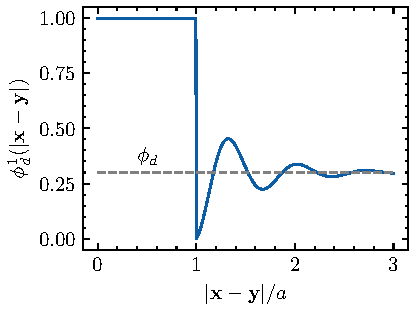
\includegraphics[width=0.2\textheight]{image/dist_phi.pdf}
    \caption{Representation of a possible form for the probability of finding the dispersed phase at \textbf{x} knowing a spherical particle of radius $a$ is present at $\textbf{y}$.
    Note the zone empty of particle concentration near the points $|\textbf{x}- \textbf{y}|=a$, this due to the impenetrability of particles. 
    }
    \label{fig:distrib}
\end{figure}
At the surface of the test-particle, the probability of finding the dispersed phase, i.e. finding the dispersed phase in contact with the surface of the reference particle, is identically null (not to be confused with the probability of finding another droplet center of mass). 
Indeed, a thin film of continuous phase always separates the droplet surface from its neighbors (see \ref{fig:distrib}).
Therefore, we may write $\phi_d^1 = 0$ at $|\textbf{x}- \textbf{y}| =a$. 
Thus, when evaluated at the subsurface of the particle, we can use the relation $\textbf{u}_f^1 = \textbf{u}^1$ and $p_f^1 = p^1$. 
Consequently, to compute the surface stress of a particle, either the conditionally-averaged quantities of the continuous phase ($\textbf{u}_f^1, p_f^1$) or the bulk quantities ($\textbf{u}^1$, $p^1$) are required. 
Another consequence of this is that, the definitions given by, \ref{eq:sigma_f_surf15}, \ref{eq:sigma_f_surf2}, or \ref{eq:sigma_f_surf} are all consistent when evaluated at the points located on the surface of the droplet at \textbf{x}. 

\subsection{Mean fields and disturbance fields contribution}

As it is often done in the literature \citep{zhang1994ensemble,jackson2000,wang2021numerical,wang2024effect}, we would like to separate the averaged momentum exchange into a contribution from the mean flow and pressure fields, and the contribution arising due to the disturbance velocity and pressure fields.  

\subsubsection{Definitions}

In the first place, we need to define what is a disturbance field.
Let us take the example of the conditioned velocity field, $\textbf{u}_f^1$, and its corresponding disturbance velocity field.
We state that the conditioned field, $\textbf{u}_f^1$, is equivalent to the ensemble-averaged velocity field $\textbf{u}_f$ when the particle at \textbf{x} is sufficiently far from the point where the velocity $\textbf{u}_f^1$ is evaluated (the point \textbf{y}).
Thus, we write,  
\begin{equation}
    \lim_{|\textbf{y}-\textbf{x}|\to\infty} 
    \textbf{u}_f^1[\textbf{y},\textbf{x},\textbf{w},t]
    =
    \textbf{u}_f[\textbf{y},t]. 
    \label{eq:lim_u_1}
\end{equation} 
Note that this definition requires an infinitely large domain. 
This implies that the solutions obtained in the subsequent sections are restricted to infinitely large domains, devoid of boundary conditions.

Let us assume that $L$ is the macroscopic length scale of our process and that $a$  is the typical size of the particles.
Since the particle-size scale $a$ is much smaller than the boundary length scale $L$ we assume that $\textsc{O}(a/L)$ is negligible. 
In the worth case scenario, the disturbance field of a droplet is $(\textbf{u}_f^1- \textbf{u}_f)\sim a/|\textbf{y}-\textbf{x}|$ \citet{kim2013microhydrodynamics}.
Hence, in a physical situation where $|\textbf{y}-\textbf{x}|\to L$ instead of $|\textbf{y}-\textbf{x}|\to\infty$ in \ref{eq:lim_u_1} we may estimate that the error is of $\mathcal{O}(a/L)$, hence negligible upon a reasonable separation of scale.
However, it is interesting to note that this will no longer be the case for other problems such as sediment transport for examples.
In this case, the boundary condition, i.e. the top of the particle bed and the ground, are at a distance of the same length scale as the particle-size. 

In light of \ref{eq:lim_u_1}, we define the disturbance velocity field as 
\begin{equation}
    \textbf{u}_f^{1d}
    =
    \textbf{u}_f^1 
    - 
    \textbf{u}_f. 
    \label{eq:def_u_1d}
\end{equation}
because it satisfies the definition, 
\begin{equation}
    \lim_{|\textbf{y}-\textbf{x}|\to\infty} 
    \textbf{u}_f^{1d}[\textbf{y},\textbf{x},\textbf{w},t]
    =
    \lim_{|\textbf{y}-\textbf{x}|\to\infty} 
    \{\textbf{u}_f^1[\textbf{y},\textbf{x},\textbf{w},t]
    - \textbf{u}_f[\textbf{y},t]\}
    = 0.
    \label{eq:lim_u_1d}
\end{equation} 
Thus, $\textbf{u}_f^{1d}$ tends to zero at large distances from the particle, which is consistent with the terminology ``disturbance''.
The definition \ref{eq:def_u_1d} can apply to any \textit{conditional-averaged} quantities $f^1$, we define
\begin{equation}
    \lim_{|\textbf{y}-\textbf{x}|\to\infty} 
    \{f_f^1[\textbf{y},\textbf{x},\textbf{w},t]
    - f_f[\textbf{y},t]\}
    =
    f_f^{1d}[\textbf{y},\textbf{x},\textbf{w},t]
    = 0.
\end{equation} 

\subsubsection{Momentum exchange decomposition}

Using the decomposition $\bm\sigma_f^1 = \bm\sigma_f^{1d} + \bm\sigma_f$ in \ref{eq:conditionally_averaged} we finally introduce the decomposition of the averaged momentum exchange term as:  
\begin{align}
    \pSavg{\bm\sigma_f^0\cdot\textbf{n}}[\textbf{x},t]
    =
    n_p[\textbf{x},t]
    \int_{|\textbf{x}-\textbf{y}|=a}
    \bm\sigma_f[\textbf{y},t]
    \cdot \textbf{n}
    d\textbf{y}
    \nonumber
    \\
    + 
    \int_{\mathbb{R}^3}
    P_1[\textbf{x},\textbf{w},t]
    \int_{|\textbf{x}-\textbf{y}|=a}
    \bm\sigma_f^{1d}[\textbf{y},\textbf{x},\textbf{w},t]
    \cdot \textbf{n}
    d\textbf{y}
    d\textbf{w}
    \label{eq:general_partition}
\end{align}
where the first term represents the contribution from the mean continuous phase stress, $\bm\sigma_f$, and the second term is the contribution from the disturbance fields stress $\bm\sigma_f^{1d}$. 
While this decomposition is arbitrary since $\bm\sigma_f^1$ could be partitioned into other arbitrary tensors, it enables by definition, the separation of the mean flow contribution, $\bm\sigma_f$, from the stress induced by the local-scale disturbance fields, $\bm\sigma_f^{1d}$.
This decomposition is used by \citet[Chapter 2]{jackson2000} and \citet{zhang1997momentum,wang2021numerical,wang2024effect} for suspensions of solid spheres, although these authors do not explicitly provide the expression for the tensor $\bm\sigma_f^{1d}$, which we aim to derive in the following sections. 

Note that $\bm\sigma_f$ is evaluated at $\textbf{y}$ in \ref{eq:general_partition}. 
Although $\bm\sigma_f$ is ensemble-averaged, we emphasize that it may still depend on the position in inhomogeneous flows. 
Assuming the suspension is slightly non-homogeneous \citep{lhuillier1992ensemble}, we have $\bm\sigma_f[\textbf{y},t] = \bm\sigma_f[\textbf{x},t] + \textbf{r}\cdot \nabla\bm\sigma_f[\textbf{x},t] + \ldots$, where $\textbf{r} = \textbf{y} - \textbf{x}$. 
By retaining only the first three terms in the expansion, we can demonstrate that
\begin{equation}
    \pSavg{\bm\sigma_f^0\cdot\textbf{n}}
    =
    n_p v_p 
    \div\bm\sigma_f
    +
    \int_{\mathbb{R}^3}
    P_1
    \int_{|\textbf{x}-\textbf{y}|=a}
    \bm\sigma_f^{1d} \cdot \textbf{n}
    d\textbf{y}d\textbf{w}.
    \label{eq:drag_final}
\end{equation}
Therefore, the total momentum exchange term contains a component related to the divergence of the mean fluid-phase stress, in addition to the contribution from the disturbance fields. 
Similar arguments can be extended to the first two moments of the hydrodynamic force. 
These expressions can be written as:
\begin{align}
    \pSavg{\textbf{r}\bm\sigma_f^0\cdot\textbf{n}}
    &=
    n_p v_p \bm\sigma_f
    +
    \int_{\mathbb{R}^3}
    P_1
    \int_{|\textbf{x}-\textbf{y}|=a}
    \textbf{r}\bm\sigma_f^{1d} \cdot \textbf{n}
    d\textbf{y}
    d\textbf{w},
    \label{eq:first_mom_general}
    \\
    \pSavg{\textbf{rr}\bm\sigma_f^0\cdot\textbf{n}}
    &=
    n_pv_p  \frac{a^2}{5} 3 [(\div \bm\sigma_f)\bm\delta]^\text{sym}
    +
    \int_{\mathbb{R}^3}
    P_1
    \int_{|\textbf{x}-\textbf{y}|=a}
    \textbf{rr}\bm\sigma_f^{1d} \cdot \textbf{n}
    d\textbf{y}
    d\textbf{w},
    \label{eq:second_mom_general}
\end{align}
where the operator $[\ldots]^\text{sym}$ returns the symmetric part of the arguments. 
It is important to note that the contribution from the mean stress in the second moment of the hydrodynamic force may become negligible when a proper separation of scale is considered. 
Indeed, this term is proportional to $a^2$ \eqref{eq:second_mom_general}, and it appears under the operator $\grad\grad\sim L^{-2}$ in the averaged momentum equation \ref{eq:dt_hybrid_rhou_f}, hence contributing to $\mathcal{O}(a^2/L^2)$, which may be considered as negligible. 

According to the expressions \ref{eq:drag_final}, \ref{eq:first_mom_general}, and \ref{eq:second_mom_general}, we will need to compute the term $\bm\sigma^{1d}_f = \bm\sigma_f^1 - \bm\sigma_f$ where $\bm\sigma_f^1$ is given by \ref{eq:sigma_f_surf}. 
Regarding the mean continuous phase stress we recall that it can be written in two ways (see \ref{chap:daniel15}), namely 
\begin{align}
    \label{eq:mean_continuous_phase_stress}
    \bm\sigma_f
    &= - p_f \bm\delta 
    + \mu_f [\pddy \textbf{u}_f+ (\pddy \textbf{u}_f)^\dagger ]
    - \frac{\mu_f}{\phi_f}\avg{\delta_\Gamma (\textbf{n}_d \textbf{u}_f'+  \textbf{u}_f' \textbf{n}_d)}, \\
    \bm\sigma_f
    &= - p_f \bm\delta 
    + \frac{\mu_f}{\phi_f} [\pddy \textbf{u}+ (\pddy \textbf{u})^\dagger ]
    - \frac{\mu_f \phi_d}{\phi_f} \textbf{e}_d
    \label{eq:mean_continuous_phase_stress2}
\end{align}
Thus using \ref{eq:sigma_f_surf} and \ref{eq:mean_continuous_phase_stress} we find for the points on the particle's surface ($|\textbf{y}-\textbf{x}| = a$) that,
\begin{align}
    \bm\sigma_f^{1d}
    =
    - p_f^{1d} \bm\delta 
    + \mu_f [\pddy \textbf{u}_f^{1d}+ (\pddy \textbf{u}_f^{1d})^\dagger ]
    + \frac{\mu_f }{\phi_f}\avg{\delta_\Gamma (\textbf{n}_d \textbf{u}_f'+  \textbf{u}_f' \textbf{n}_d)}. 
    \label{eq:sigma_explict}
\end{align}
Thus, according to \ref{eq:sigma_explict}, the disturbance stress that is integrated over the particle surface in \ref{eq:drag_final} to \ref{eq:second_mom_general}, is not only the Newtonian stress-like contribution of the disturbance fields ($\textbf{u}_f^1$ and $p_f^1$), but also includes the contribution of the term $\avg{\delta_\Gamma (\textbf{n}_d \textbf{u}_f'+  \textbf{u}_f' \textbf{n}_d)}$. 
Thus, in the force closures: \ref{eq:drag_final} and \ref{eq:first_mom_general}, we will observe the appearance of the terms involving the divergence of $\avg{\delta_\Gamma (\textbf{n}_d \textbf{u}_f'+  \textbf{u}_f' \textbf{n}_d)}$ times $n_pv_p$, and  $n_pv_p \avg{\delta_\Gamma (\textbf{n}_d \textbf{u}_f'+  \textbf{u}_f' \textbf{n}_d)}$, respectively. 
These terms will ultimately cancel out their corresponding contributions in $\bm\sigma_f$ that appear on the left-hand side of \ref{eq:drag_final} and \ref{eq:first_mom_general}. 

To provide a better understanding for the following discussion we remark that for solid particles $\textbf{e}_d = 0$. 
Therefore, subtracting \ref{eq:mean_continuous_phase_stress} from \ref{eq:mean_continuous_phase_stress2}, gives directly, 
\begin{equation}
    \avg{\delta_\Gamma (\textbf{n}_d \textbf{u}_f'+  \textbf{u}_f' \textbf{n}_d)}
    = 
    (\textbf{u}_f - \textbf{u}_d)\pddy \phi_d + \pddy \phi_d (\textbf{u}_f - \textbf{u}_d)
    -  \phi_d [\pddy \textbf{u}_d+ (\pddy \textbf{u}_d)^\dagger ]. 
    \label{eq:closure_un_nu}
\end{equation} 
Therefore, at least for solid particles, this term is non-zero as soon as there are non-negligible gradients of volume fraction and mean gradients of particle velocities. 


We conclude that the commonly used decomposition of the drag force introduced by \citet{zhang1997momentum,jackson2000}, given by \ref{eq:general_partition}, requires adding the term  $\avg{\delta_\Gamma (\textbf{n}_d \textbf{u}_f'+  \textbf{u}_f' \textbf{n}_d)}$ to the classical Newtonian stresses in the second term of \ref{eq:general_partition} and subtracting it in the mean drag force term (first term of \ref{eq:general_partition}). 
This finding implies that, in the recent work of \citet{wang2021numerical, wang2024effect}, where this decomposition is employed for the drag force, we assert that they have actually computed the integral of the first two terms of \ref{eq:sigma_explict}, while neglecting the final term. 
Interestingly, \citet{wang2024effect} specifically investigates the effect of the volume fraction gradient ($\grad \phi_d$) on the drag force. 
In this context, it is clear from \eqref{eq:closure_un_nu} that the term $\avg{\delta_\Gamma (\textbf{n}_d \textbf{u}_f'+  \textbf{u}_f' \textbf{n}_d)}$ cannot be neglected. 
Only when the analysis is accurate to $\mathcal{O}(\phi_d)$ does this term vanish in \ref{eq:drag_final}, reducing \ref{eq:sigma_explict} to the Newtonian stress expression. 
% Thus, the drag force computed in the DNS of \citet{wang2024effect} may not be the one defined in their momentum equations. 

Note that using \ref{eq:mean_continuous_phase_stress2} instead of \ref{eq:mean_continuous_phase_stress} in \ref{eq:sigma_explict} and switching $\textbf{u}_f^1$ and $\textbf{u}^1$ in \ref{eq:sigma_f_surf}, does not solve this inconsistency. 

\subsubsection{An alternative stress decomposition}

As the previous decomposition requires adding and subtracting $\avg{\delta_\Gamma (\textbf{n}_d \textbf{u}_f'+  \textbf{u}_f' \textbf{n}_d)}$ in each term of \ref{eq:general_partition}, we decide to avoid this overcomplicated operation and introduce, the partitioning 
\begin{equation}
    \bm\sigma_f^1 =
    \bm\Sigma_f + 
    \bm\Sigma_f^{1d}. 
    \label{eq:mean_Newtonian}
\end{equation}
Where the mean stress and disturbance stresses are defined as, 
\begin{align}
    \bm\Sigma_f^{1d}
    &=-p_f^{1d}\bm\delta + \mu_f^1 [\grad \textbf{u}^{1d}_f + (\grad \textbf{u}^{1d}_f)^\dagger], \\
    \bm\Sigma_f
    &=-p_f\bm\delta + \mu_f^1 [\grad \textbf{u}_f + (\grad \textbf{u}_f)^\dagger], 
\end{align}
respectively. 
Note that the use of $\textbf{u}_f$ as the ensemble-averaged velocity of reference is arbitrary.
Indeed, recall that at the surface of the test particle we have $\phi_d^1=0$, hence $\textbf{u}_f^1 = \textbf{u}^1$. 
Thus, at the surface of the test-particle, one could use the decomposition,
\begin{equation}
    \bm\sigma_f^1 =
    \bm\Sigma + 
    \bm\Sigma^{1d}. 
    \label{eq:mean_Newtonian2}
\end{equation}
Where the mean stress and disturbance stresses are defined as, 
\begin{align}
    \bm\Sigma^{1d}
    &=-p_f^{1d}\bm\delta + \mu_f^1 [\grad \textbf{u}^{1d} + (\grad \textbf{u}^{1d})^\dagger], \\
    \bm\Sigma
    &=-p_f\bm\delta + \mu_f^1 [\grad \textbf{u} + (\grad \textbf{u})^\dagger]. 
\end{align}
One could wonder which of these stress decomposition (\ref{eq:mean_Newtonian2} or \ref{eq:mean_Newtonian}) is the more efficient? 
The answer is that it depends on the unknown of the problem at hand. 
If we consider an averaged system of equations for the mean continuous phase field $\textbf{u}_f$ then, \ref{eq:mean_Newtonian} seems more adapted, however, if the unknown is \textbf{u}, then \ref{eq:mean_Newtonian2} is more adapted. 
In all case since $\textbf{u} = \textbf{u}_f + \phi_d (\textbf{u}_d - \textbf{u}_f)$ one can always recover \ref{eq:mean_Newtonian2} from \ref{eq:mean_Newtonian} or inversely.




Using the same methodology as in the previous manipulations we re-write the force closures as, 
\begin{align}
    \pSavg{\bm\sigma_f^0\cdot\textbf{n}}
    &=
    n_p v_p 
    \div\bm\Sigma_f
    +
    \int_{\mathbb{R}^3}
    P_1
    \int_{|\textbf{x}-\textbf{y}|=a}
    \bm\Sigma_f^{1d} \cdot \textbf{n}
    d\textbf{y}d\textbf{w}
    \label{eq:drag_final2}\\
    \pSavg{\textbf{r}\bm\sigma_f^0\cdot\textbf{n}}
    &=
    n_p v_p \bm\Sigma_f
    +
    \int_{\mathbb{R}^3}
    P_1
    \int_{|\textbf{x}-\textbf{y}|=a}
    \textbf{r}\bm\Sigma_f^{1d} \cdot \textbf{n}
    d\textbf{y}
    d\textbf{w}
    \\
    \pSavg{\textbf{rr}\bm\sigma_f^0\cdot\textbf{n}}
    &=
    n_pv_p  \frac{a^2}{5} 3 [(\div \bm\Sigma_f)\bm\delta]^\text{sym}
    +
    \int_{\mathbb{R}^3}
    P_1
    \int_{|\textbf{x}-\textbf{y}|=a}
    \textbf{rr}\bm\Sigma_f^{1d} \cdot \textbf{n}
    d\textbf{y}
    d\textbf{w}
    \label{eq:second_mom_general2}
\end{align}
This decomposition, though perhaps less natural, appears to be more physically meaningful. 
Indeed, unlike the previous approach, the mean contribution no longer depends on the mean relative motion through the term $\avg{\delta_\Gamma (\textbf{n}_d \textbf{u}_f'+  \textbf{u}_f' \textbf{n}_d)}$ in $\bm\sigma_f$ (see \ref{eq:closure_un_nu}), but solely on the mean fluid phase properties $p_f$ and $\textbf{u}_f$, while the local stress is a Newtonian-like stress.  

The main take-away of this section is that: (1)  the particle-averaged force traction terms can be computed based on the knowledge of $p_f^{1d}$ and $\textbf{u}_f^{1d}$. 
These fields can be obtained by solving the corresponding disturbance field equations. 
Note that one may also compute the mixture properties $p^{1d}$ and $\textbf{u}^{1d}$ and then use the relation $p_f^{1d} = p^{1d} + \phi_d (p_f - p_d)$ or $\textbf{u}_f^{1d} = \textbf{u}^{1d} + \phi_d (\textbf{u}_f - \textbf{u}_d)$. 
And (2) the force decomposition often used \citep{jackson2000,zhang1997momentum,wang2021numerical,wang2024effect} seems inconsistent compared to the drag force computed in the cited studies.
Indeed, it is likely that their definition of the ``drag force'' term, requires the subtraction of a term proportional to the particle volume fraction. 
This inconsistency is settled by re-defining the forces partition.  

\subsection{Particle phase volumic terms}

Some closure terms such as the particle internal stress $\pOavg{\bm{\sigma}_2^0}$ or the particle internal dissipation term $\pOavg{\bm{\sigma}_2^0:\grad \textbf{u}_d^0}$ are particle-averaged volume integral of locals quantities. 
In this situation the reformulation is slightly different since we must consider volume and not the surfaces of the particle.  Nevertheless the approach is similar. 
For the particle internal stress we can write, 
\begin{equation}
    \pOavg{\bm\sigma_d^0}[\textbf{x},t]
    =
    \int_{\mathbb{R}^3}
    P_1[\textbf{x},\textbf{w}]
    \int_{|\textbf{x}-\textbf{y}|<a}
    \bm\sigma_d^1[\textbf{y},t;\textbf{x},\textbf{w}] 
    d\textbf{y}
    d\textbf{w}. 
    \label{eq:conditionally_averaged_vol}
\end{equation}
Assuming a Newtonian fluid for the particles, $\bm\sigma_d^0 = -p_d^0 \bm\delta + \mu_d [\nabla \textbf{u}_d^0 + (\nabla \textbf{u}_d^0)^\dagger]$, and given that within the region $|\textbf{x} - \textbf{y}| < a$, only the dispersed phase is present.
This allows the permutation between ensemble averages and derivatives.
We can express this as:
\begin{equation}
    \bm\sigma_d^1  
    = 
    -p_d^1   \bm\delta
    + \mu_d  [\pddy \textbf{u}^1_d+(\pddy  \textbf{u}^1_d)^\dagger],
    \label{eq:dispersed_phase_stress}
\end{equation}
which is simply the expression of the Newtonian stress within the particle centered at \textbf{x}, based on the mean fields $p_d^1$ and $\textbf{u}_d^1$. 
As in the previous section, one can eventually partition this conditional stress into an ensemble averaged stress plus a local disturbance field. 

\subsection{Continuous phase closures}

The closure terms of the form $\avg{\chi_f f_f^0}$ differ in their mathematical structure, as they represent an average over the continuous phase rather than the dispersed phase. 
Consequently, the reformulation method is slightly different and requires additional assumptions. Two examples of such terms are the Reynolds stress $\avg{\chi_f \textbf{u}_f'\textbf{u}_f'}$ and the fluid-phase dissipation $\avg{\chi_f \bm\sigma_f^0 : \nabla \textbf{u}_f^0}$, which appear in \ref{eq:dt_hybrid_rhou_f} and \ref{eq:dt_hybrid_k1}, respectively.  

We first note that, 
\begin{equation}
    \frac{1}{N}\sum_\alpha^N
    \int_{\mathbb{R}^3}
    \int_{\mathbb{R}^3}
    \delta(\textbf{y}-\textbf{x}_\alpha[\FF,t])
    \delta(\textbf{w}-\textbf{u}_\alpha[\FF,t])
    d\textbf{x}
    d\textbf{w}
    = 1,
\end{equation}
where $N$ is the total number of particles in the flow. 
Using this relation one may re-formulate the ensemble average of a continuous phase quantity as 
\begin{equation}
    \phi_f f_f[\textbf{x},t]
    = 
    \frac{1}{N}
    \int_{\mathbb{R}^3}
    \int_{\mathbb{R}^3}
    f_f^1[\textbf{x},\textbf{y},\textbf{w},t] \phi_f^1[\textbf{x}|\textbf{y},\textbf{w},t]  P_1[\textbf{y},\textbf{w}] 
    d\textbf{y} 
    d\textbf{w}
    \label{eq:conditional_averaged_fluid}
\end{equation}
where,
\begin{equation*}
    f_f^1[\textbf{x},\textbf{y},\textbf{w},t] \phi_f^1[\textbf{x}|\textbf{y},\textbf{w},t]  P_1[\textbf{y},\textbf{w}]
    =     
    \avg{
    \sum_\alpha^N 
    \delta(\textbf{y}-\textbf{x}_\alpha[\FF,t])
     \delta(\textbf{w}-\textbf{u}_\alpha[\FF,t])
    (\chi_f
    f^0_f)[\textbf{x},t;\FF]
    }.
\end{equation*}
In this expression $f_f^1[\textbf{x},t;\textbf{y},\textbf{w}]$ is the average of the local quantity $f_f^0$ evaluated at $\textbf{x}$ and time $t$ conditionally on, the presence of the continuous phase at \textbf{x}, and a particle center of mass at $\textbf{y}$ with center of mass velocity $\textbf{w}$. 
Similarly, $\phi_f^1[\textbf{x},t|\textbf{y},\textbf{w}]$ is the fluid phase volume fraction at \textbf{x} and time $t$, conditionally on the presence of a particle at $\textbf{y}$ with center of mass velocity \textbf{w}. 
Note that for $|\textbf{x} - \textbf{y}| < a$, $\phi_f^1[\textbf{y}|t,\textbf{x},\textbf{w}] = 0$ however at, 
$\lim_{|\textbf{x} - \textbf{y}| \to \infty} \phi_f^1 = \phi_f$. 
Note that this derivation is consistent with (2.21) and (2.22) of \citet{zhang1994ensemble} with $K = 1$. 

This, formulation remains quite general and is valid regardless of the flow regime, however, the presence of the term $N$ makes this formulation unpractical. 
Indeed, $P_1 = n_p[\textbf{y},t] P_1[\textbf{w}|\textbf{y},t]$ and $n_p[\textbf{y},t] /N = V_\Omega$, where $V_\Omega$ is the volume of the whole domain. 
Thus, substituting  $n_p[\textbf{y},t] /N = V_\Omega$ into \ref{eq:conditional_averaged_fluid} transforms the right-hand side of this relation to a volume average over $V_\Omega$ of a property evaluated at \textbf{x} on all possible particles positions in $V_\Omega$.  
Anyhow, \ref{eq:conditional_averaged_fluid} requires macroscopic information such as $N$ and $V_\Omega$, which we do not necessarily have if our goal is to compute general closure formulation. 
This is because, contrary to particle-averaged quantities, we could not consider a contribution per particle that is holds fixed at \textbf{x}, but the action of all particles on a given property of the fluid at \textbf{x}.
In other words, the integration variable is on the particle center of mass position in \ref{eq:conditional_averaged_fluid}, while in \ref{eq:conditionally_averaged} it is on the local non-averaged properties while the particle position remains fixed. 

Consequently, we adopt the approach proposed by \citet{batchelor1972sedimentation} and reformulate \ref{eq:conditional_averaged_fluid} based on the additivity assumption \footnote{
    This implicitly assumes that $f_f^0$ is governed by a linear equation. 
    That is the case for the Stokes flow regime, or unsteady Stokes flow regime if $f_f^0$ is the velocity. 
}. 
Thus, we postulate that $f_f^0[\textbf{x},t;\FF]$ can be subdivided into $N$ contributions, namely:  
\begin{equation}
    f_f^0[\textbf{x},t;\FF]
    = 
    \sum_\alpha^N
    f_{f_\alpha}^0[\textbf{x},t;\FF]
    + f_{f_0}^0[\textbf{x},t;\FF]
\end{equation}
where $f_{f_\alpha}^0$ is the disturbance fields produced by the particle $i$ on $f_f^0$ and $f_{f_0}^0$ is the undisturbed background flow. 
This implies that $f_{f}^0 = f_{f_0}^0$ in the absence of particle in the flow. 
Under this assumption, we can write, 
\begin{equation}
    \avg{\chi_f f_f^0}[\textbf{x},t]
    = 
    \int_{\mathbb{R}^3} 
    \avg{
        \sum_\alpha^N 
    (\chi_f f_{f_\alpha}^0)[\textbf{x}_\alpha + \textbf{r},t,\FF] \delta(\textbf{x} - \textbf{x}_\alpha[\FF,t] - \textbf{r})}d\textbf{r}
    +( \phi_f f_{f_0})[\textbf{x},t]
    \label{eq:first_step_additivity}
\end{equation}
Where $\phi_f f_{f_0}[\textbf{x},t]$ is the mean background flow, and were we have used a relation similar to the one presented in \ref{app:expansion}, to reformulate the first term of \ref{eq:first_step_additivity}. 
Then, we use the Taylor expansion, $\delta(\textbf{x} - \textbf{x}_\alpha - \textbf{r}) =\delta(\textbf{x} - \textbf{x}_\alpha) - \textbf{r}\cdot \grad\delta(\textbf{x} - \textbf{x}_\alpha)+ \ldots$, on the first term on the right-hand side of \ref{eq:first_step_additivity}.
This gives,  
\begin{align}
    \avg{\chi_f f_f^0}[\textbf{x},t]
    = 
    \phi_f f_{f_0}[\textbf{x},t]
    + 
    \int_{\mathbb{R}^3} 
    \int_{\mathbb{R}^3} 
    (f_{f_p}^1\phi_f^1) [\textbf{y}|\textbf{x},\textbf{w},t] P_1[\textbf{w},\textbf{x}]
    d\textbf{r}
    d\textbf{w}
    \nonumber \\
    + 
    \div 
    \int_{\mathbb{R}^3} 
    \int_{\mathbb{R}^3} 
    \textbf{r}
    (f_{f_p}^1\phi_f^1) [\textbf{y}|\textbf{x},\textbf{w},t] P_1[\textbf{w},\textbf{x}]
    d\textbf{r}
    d\textbf{w}
    + \ldots
    % + \grad^n 
    % \int_{\mathbb{R}^6} 
    % \mathcal{O}(\textbf{r}^n)
    % (f_{f_p}^1\phi_f^1) [\textbf{y}|\textbf{x},\textbf{w},t] P_1[\textbf{w},\textbf{x}]
    % d\textbf{r}
    % d\textbf{w}
    \label{eq:f_f_1_def}
\end{align}
with, 
\begin{equation}
    (f_{f_p}^1 \phi_f^1) [\textbf{y}|\textbf{x},\textbf{w},t] P_1[\textbf{w},\textbf{x}]
    = 
    \avg{
    \sum_\alpha
    \chi_f f_{f_\alpha}^0[\textbf{x}_\alpha + \textbf{r},t;\FF] 
    \delta(\textbf{x} - \textbf{x}_\alpha[\FF,t])
    \delta(\textbf{w} - \textbf{u}_\alpha[\FF,t])
    }. 
\end{equation}
In this definition $f_{f_p}^1$ is the averaged value of the disturbance fields at $\textbf{x}+\textbf{r}$, produced by the particle at $\textbf{x}$, in opposition to $f_f^1$ \eqref{eq:conditional_averaged_fluid} which is the averaged value of $f_f^0$ evaluated at \textbf{x}, conditionally on the presence of an arbitrary particle at \textbf{y}.
Assuming a situation where there is no background flow (such as in the case of sedimenting particle in an otherwise quiescent flow), a homogeneous situation, and in the dilute limit, such that $\phi_f^1 = \phi_f$ when $|\textbf{x}-\textbf{y}|>a$ and $\phi_f^1 =0$ when $|\textbf{x}-\textbf{y}|<a$, we obtain, 
\begin{equation}
    f_f[\textbf{x},t]
    = 
    \int_{\mathbb{R}^3} 
    P_1[\textbf{x},\textbf{w}] 
    \int_{|\textbf{x}-\textbf{y}| >a} 
    f_{f_p}^1[\textbf{x}+ \textbf{r}| \textbf{x}]
    d\textbf{r}
    d\textbf{w}
    + 
    \text{Error}
    \label{eq:Batchelor2}
\end{equation}
\begin{equation}
    \text{Error}
    = 
    \int{
    \mathcal{O}(|\textbf{r}| f_{f_p}^1  n_p / L)
    } d\textbf{r}. 
    \label{eq:error0}
\end{equation}
Note that in \ref{eq:error0} we have expressed explicitly the error generated due to the Taylor expansion of the Dirac delta: $\delta(\textbf{x} - \textbf{x}_\alpha - \textbf{r})$. 
Indeed, at the leading order we find, $\delta(\textbf{x} - \textbf{x}_\alpha - \textbf{r}) =\delta(\textbf{x} - \textbf{x}_\alpha) +  \mathcal{O}(|\textbf{r}|/L)$, where $L$ is the typical length of the macroscopic flow variation.
Assuming that $\text{Error}= \mathcal(\phi_d^2)$ rather than \ref{eq:error0} in \ref{eq:Batchelor2}, we find that \ref{eq:Batchelor2} is exactly equation (2.10) of \citet{batchelor1972sedimentation}. 
\citet{batchelor1972sedimentation} uses such a formula to compute the mean fluid phase velocity at a given point in the fluid, conditionally on the presence of a particle at a certain distance from this point. 
Consequently, \ref{eq:Batchelor2} provides an extension of Eq (2.10) of \citet{batchelor1972sedimentation}, in the sense that we give an explicit expression of the``Error'' term \eqref{eq:error0}. % based on mathematical arguments, rather than Batchelor's physical arguments. 
Additionally, \ref{eq:f_f_1_def} is a generalization of \ref{eq:Batchelor2} when the homogeneous hypothesis, as well as the dilute hypothesis, are not assumed. 



As discussed in \citet{batchelor1972sedimentation}, the first integral in \ref{eq:f_f_1_def} may diverge if the disturbance field $f_{f_p}^1$ does not decay rapidly enough as $|\textbf{r}|$ approaches infinity. 
We believe that, in cases where $f_{f_p}^1$ does not decay sufficiently fast as $|\textbf{r}|$ increases, the ``Error'' in \ref{eq:Batchelor2} also tends to infinity since we integrate a term proportional to $f_{f_p}^1 |\textbf{r}|$ which is even more divergent for large $|\textbf{r}|$. 
Thus, we argue that Batchelor's original formula is not accurate at $\mathcal{O}(\phi_d^2)$, but rather at $\mathcal{O}(|\textbf{r}| f_{f_p}^1  n_p / L)$, making \ref{eq:Batchelor2} unable to produce physical results when $f_{f_p}^1$ does not decay rapidly since the ``Error'' also tends to infinity in these cases. 
In cases where the first integral on the right-hand side converges, but the "Error" does not, the results must still be considered with caution, though the first integral is. 


Additionally, we believe that in the general case, where $f_f$ is given by \ref{eq:f_f_1_def}, it is impossible to obtain meaningful results with the latter formula. 
Indeed, \ref{eq:f_f_1_def} requires the use of the Taylor expansion, $\delta(\textbf{x} - \textbf{x}_\alpha - \textbf{r}) =\delta(\textbf{x} - \textbf{x}_\alpha) - \textbf{r}\cdot \grad\delta(\textbf{x} - \textbf{x}_\alpha)+ \ldots + \mathcal{O}(\textbf{r}^n/L^n)$. 
Additionally, in the integrals of \ref{eq:f_f_1_def}, \textbf{r} is evaluated from the particle center to an infinitely large distance from it.
Thus, it is evident that for any unbounded $f_{f_p}^1$, when $|\textbf{r}| \to \infty$, there is always an arbitrary integer $n$ for which, $\int f_{f_p}^1 \phi^1_f \textbf{r}^n d\textbf{r} \to \infty$.
Thus, if one considers a sufficiently high order moment in \ref{eq:f_f_1_def}, he will end up including a divergent integral. 
Following the same argument we can show that the  ``Error'' term included due to the Taylor expansion, proportional to $\mathcal{O}(f_{f_p}^1 r^n /L^n)$ might diverge as well since $r$ goes to infinity and $L$ stays constants. 
Consequently, in the inhomogeneous situations, and for unbounded functions $f_{f_p}^1$, we state that \ref{eq:f_f_1_def} might be not relevant as it produces divergent integral and an infinite ``Error'' as well. 

Note that the wake of a spherical particle in an unbounded fluid in Stokes flow, yields a velocity field $\textbf{u}_{f_p}$ proportional to  $\sim 1/|\textbf{r}|$. 
Thus, such a velocity field is a good example of a situation where: the continuous phase properties $f_{f_p}^1$ is unbounded, the first integral and the ``Error'' in \ref{eq:Batchelor2} diverge. 
In such cases, Batchelor used the renormalization method to circumvent these difficulties. 
% Note that these problems of divergent integral could be guessed well in advance since the Taylor expansion of $\delta(\textbf{x} - \textbf{x}_\alpha - \textbf{r})$ for a vector $\textbf{r}$ that is arbitrarily large doesn't make
% Nevertheless, such manipulation is required to demonstrate Batchelor's original formula and its generalization given by \eqref{eq:Batchelor2}. 


 
In conclusion, \ref{eq:Batchelor2}  is meaningful only for fields that respect the following conditions: 
(1) The influence of the particles on the field $f_f^0$ must be additive, this is the case when ${f_f^0}$ follows the Stokes equations; 
(2) The closures must be derived in a homogeneous flow, such that the higher moments in \ref{eq:f_f_1_def} cancel exactly. 
And (3), the integral over $\mathbb{R}^3$ of the term $|\textbf{r}| f_{f_p}^1$ must be finite, such that \ref{eq:Batchelor2} remains finite. 
Even if \ref{eq:Batchelor2} is not ideal, we will be using this relation to compute the continuous phase closures since for instance, this is the only tool that we have. 
Note that a new method will be presented in \ref{chap:pseudoturbulence} where we use \textit{The Nearest particle statistics} \citep{zhang2021ensemble} to compute these kinds of ensemble-averaged terms, but without the need for such approximations.


\section{Single-particle ensemble averaged problem}
\label{sec:the_disturbance_eq}

Now that we have proved the link between the ensemble-averaged closures and the conditional averaged quantities, we present the corresponding equations for these averaged conditional quantities. 
For all the closure related to the momentum equations, we need to find: $\textbf{u}^{1d}$ and $p^{1d}$ or $\textbf{u}^{1d}_f$ and $p^{1d}_f$. 
To that end, we follow \citep{hinch1977averaged,zhang1994averaged} and derive the \textit{single-particle} conditioned Navier-Stokes equations.
It turns out that deriving the \textit{single-particle} conditioned Navier-Stokes equations in a form like \ref{eq:dt_avg_rhou} is considerably simpler than using the \textit{Favre} averaged formulation or two-fluid formulation. 
Thus, in the following, we provide a set of equations for $\textbf{u}^{1d}$ and $p_f^{1d}$. 

We recall that the \textit{single-fluid} formulation of the Navier-Stokes equations, can be written at the local scale as (see \ref{ap:momentum_formulation}),
\begin{align}
    \label{eq:dt_local_mass}
    \div \textbf{u}^0 = 0, \\
    \pddt \textbf{u}^0
    + \div (\textbf{u}^0\textbf{u}^0 - \bm\sigma^*)
    &= \textbf{g}
    +(\kappa/\rho_f)(\bm\sigma_f^0\cdot \textbf{n})\delta_\Gamma,
    \label{eq:dt_local}
\end{align}
Where we noted $\textbf{u}^0 = \chi_f \textbf{u}f^0 + \chi_d \textbf{u}_d^0$, and $\bm\sigma^* = (\chi_f \bm\sigma_f^0 + \chi_d \bm\sigma_d^0/\zeta + \delta_\Gamma \bm\sigma_\Gamma^0/\zeta )/\rho_f $ referred as the density-weighted stress.
$\bm\sigma_{f,d}^0 = -p_{f,d}^0\bm\delta + \mu_{f,d}\left[\grad \textbf{u}_{f,d}^0+ (\grad \textbf{u}_{f,d}^0)^\dagger\right]$ denote the Newtonian stresses and $\bm\sigma_\Gamma^0 = \gamma (\bm\delta - \textbf{nn})$ represents the surface tension stress. 
We introduced $\kappa = (1-\zeta)/\zeta$ and $\zeta = \frac{\rho_d}{\rho_f}$ as the density ratio, consequently the interface exchange term vanishes for iso-dense suspensions. 
The boundary conditions at the surface of the droplets are implicitly included in the \textit{single-fluid} formulation \eqref{eq:dt_local}; however, it will be useful to recall them here for later reference, 
\begin{align}
    \label{eq:dt_rho_I3}
    \textbf{u}_f^0 = \textbf{u}_d^0 = \textbf{u}_\Gamma^0, \\
    \Jump{\bm{\sigma}_k^0} 
    =
    -\gamma\textbf{n}(\div \textbf{n}). 
    \label{eq:dt_rho_I2}
\end{align}

To obtain an equation for the disturbance velocity fields $\textbf{u}^{1d}$ we remark that this field can be defined by the operation, 
\begin{equation}
    \avg{(\delta_1 - P_1) \textbf{u}^0}
    =
    \avg{\delta_1 \textbf{u}^0}
    - \avg{P_1 \textbf{u}^0}
    = 
    P_1 \textbf{u}^1
    - P_1 \textbf{u}
    = P_1 \textbf{u}^{1d}. 
    \label{eq:first_step_u0}
\end{equation}
Note that $\textbf{u}^0$ and \ref{eq:dt_local} are evaluated at the point \textbf{x} while the Dirac function, 
\begin{equation}
    \delta_1[\textbf{y},\textbf{w},t,\FF] = \sum_\alpha^N \delta(\textbf{x}_\alpha[\FF,t]-\textbf{y})\delta(\textbf{u}_\alpha[\FF,t] - \textbf{w}),
\end{equation}
expresses the condition of having a particle at \textbf{y} with velocity \textbf{w}, and is therefore independent of \textbf{x}. 
In opposition to the definition given by \ref{eq:delta_1} we now consider that the particle center of mass is at \textbf{y}. 
From \ref{eq:first_step_u0}, we deduce that the momentum conservation equation for $\textbf{u}^{1d}$ is obtained by multiplying \ref{eq:dt_local} by $\delta_1 - P_1$ and averaging over all configurations. 
However, since $\delta_1$ is still a function of time $t$, this operation will require a conservation equation for $\delta_1$ and $P_1$ as well.  

Taking the partial time derivative of $\delta_1$ yields directly the relation, 
\begin{equation}
    \pddt\delta_1 
    + \pddy\cdot(\textbf{w}\delta_1)
    + \pddw\cdot(\textbf{a}_\alpha\delta_1)
    = 0 
    \label{eq:dt_delta_1}
\end{equation}
where $\textbf{a}_\alpha[\FF,t] = \pddt \textbf{u}_\alpha[\FF,t]$ is the acceleration of the particle $i$ in the configuration $\FF$. 
Ensemble averaging this equation yields an equation for  $P_1[\textbf{x},\textbf{w},t]$ which reads, 
\begin{equation}
    \pddt P_1
    + \pddy\cdot(\textbf{w}  P_1)
    + \pddw\cdot(\textbf{a}_p P_1)
    = 0.
    \label{eq:dt_P_1}
\end{equation}
Where $\textbf{a}_p = \avg{\delta_1 \textbf{a}_\alpha}/P_1$ is the mean acceleration of the center of mass of velocity \textbf{w}. 
This equation is a conservation equation of the one-point statistics: $P_1$,  along its phase space formed by $\textbf{y},\textbf{w},t$. 
Note that integrating \ref{eq:dt_P_1} over $\textbf{w}$ yields a conservation equation for the number density $n_p[\textbf{y},t]$, because of \ref{eq:Pw_normed}.  

\subsection{Single-particle conditionally averaged  Navier-Stokes equations}

% \tb{
%     If $\delta_1$ wheer express in terms of $x + r$ instead? 
%     \begin{align}
%         \pddt (P_1 \textbf{u}^{1d})
%         + \div \avg{(\textbf{u}^0 \textbf{u}^0 - \bm\sigma^*)(\delta_1 - P_1)} 
%         + \div \avg{(\delta_1 - P_1)\textbf{u}^0 \textbf{w}}\nonumber \\ 
%         + \pddw\cdot \avg{(\delta_1\textbf{a}_\alpha - P_1\textbf{a}_p) \textbf{u}^0}
%         =  (\kappa / \rho_f) \avg{ (\delta_1 - P_1) \delta_\Gamma \bm\sigma_f^0\cdot \textbf{n}},
%         + \avg{(\textbf{u}^0 \textbf{u}^0 - \bm\sigma^*)\cdot \grad(\delta_1 - P_1) }
%     \end{align}
% }

Multiplying \ref{eq:dt_local_mass} and \ref{eq:dt_local} by $(\delta_1 - P_1)$ and using \ref{eq:dt_delta_1},  \ref{eq:dt_P_1} yields the general form of the \textit{single-particle} conditionally-averaged \textit{single-fluid} formulation of the Navier-Stokes equations, namely,  
\begin{align}
    P_1 \div \textbf{u}^{1d}
    = 0 
    \label{eq:conditional_eqs_mass}
    \\
    \pddt (P_1 \textbf{u}^{1d})
    + \div \avg{(\textbf{u}^0 \textbf{u}^0 - \bm\sigma^*)(\delta_1 - P_1)} 
    + \pddy\cdot\avg{(\delta_1 - P_1)\textbf{u}^0 \textbf{w}}\nonumber \\ 
    + \pddw\cdot \avg{(\delta_1\textbf{a}_\alpha - P_1\textbf{a}_p) \textbf{u}^0}
    =  (\kappa / \rho_f) \avg{ (\delta_1 - P_1) \delta_\Gamma \bm\sigma_f^0\cdot \textbf{n}},
    \label{eq:conditional_eqs}
\end{align}
We can observe that the only differences with \ref{eq:conditional_eqs} and \ref{eq:conditional_eqs_mass} and their local counterpart is the presence of the factor $(\delta_1 - P_1)$ in front of all the terms, (which represent the constraint of having a particle at \textbf{y}), and the additional advecting terms on the left-hand side of \ref{eq:conditional_eqs}. 
Note that the gravity acceleration term canceled out in \ref{eq:conditional_eqs} since $\avg{(\delta_1 - P_1)\textbf{g}} = (P_1 -P_1 )\textbf{g} =0$. 
This simply means that in the reference frame of $\textbf{u}^{1d}$ the gravity acceleration does not play any role.
This is easily explained, as \ref{eq:conditional_eqs} represents the momentum equation for $\textbf{u}^{1}$, minus the one for $\textbf{u}$, both of which are subject to the body force \textbf{g}.
Even though the goal is not to solve \ref{eq:conditional_eqs} in all its generality, reformulating the terms in \ref{eq:conditional_eqs} and \ref{eq:conditional_eqs_mass} can be useful for gaining physical insight. 


Although we did not explicitly write all the terms of \ref{eq:conditional_eqs} and \ref{eq:conditional_eqs_mass} yet, we can already note some interesting features. 
First, using \ref{eq:examples1},  \ref{eq:conditional_eqs_mass} can be written as $P_1 \div \textbf{u}^{1d} =0$, indicating that the averaged bulk disturbance field around the particle is divergence-free.  

\subsubsection{Advecting terms}

We begin by reformulating the advecting terms of \ref{eq:conditional_eqs}.
Using the definition of $\textbf{u}^{1d}$ we can write, 
\begin{align}
    \label{eq:examples1}
    \avg{(\delta_1 - P_1) \textbf{u}^0}
    &= P_1 \textbf{u}^{1d},\\ 
    \avg{(\delta_1 - P_1)\textbf{u}^0 \textbf{w}}
    &= \avg{(\delta_1 - P_1)\textbf{u}^0 }\textbf{w} 
    = P_1\textbf{u}^{1d}\textbf{w} \\
    \label{eq:examples2}
    \avg{(\delta_1 - P_1)\textbf{u}^0 \textbf{u}^0}
    &= 
    P_1 (\textbf{u}^1\textbf{u}^1 - \textbf{u}\textbf{u})
    + \avg{\delta_1 \textbf{u}''\textbf{u}''}
    - P_1 \avg{ \textbf{u}'\textbf{u}'}
    \nonumber\\
    &= 
    P_1 (\textbf{u}^{1d}\textbf{u}^{1d} + \textbf{u}\textbf{u}^{1d}+  \textbf{u}^{1d}\textbf{u})
    + \avg{\delta_1 \textbf{u}''\textbf{u}''}
    - P_1 \avg{ \textbf{u}'\textbf{u}'}
    \\
    \avg{(\delta_1\textbf{a}_\alpha - P_1\textbf{a}_p) \textbf{u}^0}
    &=
    P_1\textbf{a}_p \textbf{u}^{1d}
    + \avg{\delta_1\textbf{a}_\alpha' \textbf{u}^0} 
    % \\
    % \rho_f \avg{(\delta_1 - P_1) \bm\sigma^*} 
    % &= 
    % \avg{(\delta_1 - P_1) [\chi_f \bm\sigma^0_f]} 
    % \avg{(\delta_1 - P_1) [\chi_d \bm\sigma^0_d +\delta_\Gamma \bm\sigma_\Gamma^0]/\zeta } 
    \label{eq:examples}
\end{align}
We recall that $\textbf{u}'' = \textbf{u}^0 - \textbf{u}^1$, thus the terms $\avg{\delta_1 \textbf{u}''\textbf{u}''}$ corresponds to the fluctuations of the velocity at \textbf{x} over all configuration where a particle is at \textbf{y} with velocity \textbf{w}, while $\avg{ \textbf{u}'\textbf{u}'}$ is the classic \textit{Reynolds stress} tensor evaluated at \textbf{x}. 
Similarly, $\avg{\delta_1\textbf{a}_\alpha' \textbf{u}^0}$ is the covariance between the particle center of mass acceleration located at \textbf{y} and the local bulk velocity evaluated at \textbf{x}. 



In \ref{eq:examples} we can observe the presence of the conditional field $\textbf{u}^{1d}$ and the ensemble-averaged velocity $\textbf{u}$. 
This implies that there is a coupling between the disturbance field $\textbf{u}^{1d}$, which is the local field describing the disturbance flow around a particle (at \textbf{y}), and the mean flow \textbf{u}.
Indeed, we can identify in \ref{eq:examples2} the advecting term $\textbf{u}^{1d}\textbf{u}^{1d}$ which represents the inertial effect due to the relative velocity scale $\textbf{u}^{1d} \sim \textbf{w}- \textbf{u}$, and the fluxes $\textbf{u}^{1d}\textbf{u}$, which represents the inertial effect due to the moving ``reference frame'' (moving with the velocity \textbf{u}). 
Thus, at finite \textit{Reynolds number}, not only the relative inertia between the test-particle and bulk the bulk matter but also the mean motion of the reference frame, moving with velocity \textbf{u}. 


\citet{maxey1983equation}, derive the Navier-Stokes equation written in the reference frame of a particle immersed in a pure solvent. 
We can observe that Eq. (15) of \citet{maxey1983equation} posses nearly the same advecting terms that the first three terms in \ref{eq:examples2}. 
It will be demonstrated that the equivalence between \ref{eq:examples2} and Eq. (15) of \citet{maxey1983equation} will be exact only in the dilute regime. 
In any case, this resemblance implies that, due to the application of the operator $\avg{(\delta_1-P_1)\ldots}$ on the Navier-Stokes equations, \ref{eq:conditional_eqs} is equivalent to the Navier-Stokes equations formulated in the reference frame of a particle at \textbf{y} with velocity \textbf{w}.
However, instead of having a particle immersed in a pure solvent, here the test particle is immersed in an equivalent medium, with additional stresses $\avg{\delta_1 \textbf{u}''\textbf{u}''}$ and $\avg{\delta_1\textbf{a}_\alpha' \textbf{u}^0}$. 


The terms related to the mean particles' acceleration $\textbf{a}_p$ or the particles relative acceleration $\textbf{a}_\alpha'$ witness of the fact that statistically, the fluctuation of the particles acceleration contribute to the mean forces governing the mixture around the test-particles at \textbf{y} with velocity \textbf{w}. 

\subsubsection{Stresses terms}

Now let us focus on the Newtonian stresses and the interface exchange terms. 
Using the local definition of the Newtonian stresses we can write, 
\begin{align}
    \avg{\bm\sigma^* (\delta_1 - P_1)} \rho_f
    &= \avg{\chi_f \bm\sigma^0_f (\delta_1 - P_1)}
    + \avg{[\chi_d \bm\sigma^0_d  + \delta_\Gamma \bm\sigma^0_\Gamma] (\delta_1 - P_1)}/\zeta
    \nonumber \\
    &= 
    - P_1 [
        \phi_f^1 p_f^1
        - \phi_f p_f
    ]\bm\delta
    + P_1 \mu_f [\grad \textbf{u}^{1d}+(\grad \textbf{u}^{1d})^\dagger] \nonumber \\
    &+ \avg{[\chi_d (\bm\sigma_d^0 - 2 \mu_f \textbf{e}^0_d ) + \chi_\Gamma \bm\sigma_\Gamma ]  (\delta_1 - P_1)}/\zeta \nonumber \\
    &= 
    - P_1  p_f^{1d}\bm\delta
    \label{eq:equivalent_stress}
    + P_1 \mu_f [\grad \textbf{u}^{1d}+(\grad \textbf{u}^{1d})^\dagger] \\
    &+P_1 [\phi_d^1 p_f^1
    - \phi_d p_f]\bm\delta
    + \avg{[\chi_d (\bm\sigma_d^0 - 2 \mu_f \textbf{e}^0_d \zeta) + \chi_\Gamma \bm\sigma_\Gamma ]  (\delta_1 - P_1)} /\zeta \nonumber
\end{align}
The first equality is obtained by direct use of the density-weighted stress introduced above, the second by using the definition of a Newtonian stress, and the third one by using the identity $\phi_f^1 =1  - \phi_d^1$, $\phi_f = 1 -\phi_d$ and $\phi_f^{1d} = (1 - \phi_d^1) - (1 - \phi_d) = \phi_d^{1d}$. 

According to \ref{eq:equivalent_stress}, the mean stress governing the disturbance field $\textbf{u}^{1d}$ has the form of a Newtonian stress (see the terms of the first lines), and a contribution related to the presence of the particle in the mixture (see the terms on the second lines). 
% Particularly, note that the presence of the term $p_f \phi_d^{1d}$, in the stress indicates that even the absolute pressure $p_f$ plays a role in the behavior of the disturbance fields when $\phi_d^{1d} = \phi_d^1 - \phi_d$ is non-zero. 
% However, we can remark that this contribution will be balanced partly by the particle phase contribution. 

The particle exchange of momentum (on the right-hand side of \ref{eq:conditional_eqs}) can be expressed in a hybrid form using the classic Taylor expansion method on the distribution $\delta_\Gamma$, it yields 
\begin{equation}
    \avg{ (\delta_1 - P_1) \delta_\Gamma \bm\sigma_f^0\cdot \textbf{n}}
    = \avg{ (\delta_1 - P_1) \delta_p \intO{\bm\sigma_f^0\cdot \textbf{n}}}
    - \div \avg{ (\delta_1 - P_1) \delta_p \intO{\textbf{r}\bm\sigma_f^0\cdot \textbf{n}}}
    + \ldots
    \label{eq:drag_force_term}
\end{equation}
We recall that in this definition $\delta_p = \sum_\alpha^N\delta(\textbf{x}_\alpha - \textbf{x})$ while $\delta_1 = \sum_\alpha^N\delta(\textbf{x}_\alpha - \textbf{y})\delta(\textbf{u}_\alpha - \textbf{w})$.  
Thus, the first term on the right-hand side of \ref{eq:drag_force_term} corresponds to the mean drag force at \textbf{x} averaged on every configuration where a particle is at \textbf{y}, minus the mean drag force at \textbf{x} times $P_1$, averaged on every configuration. 
Thus, it corresponds to the drag force contribution uniquely due to the average particle-particle interaction, i.e. the additional drag due to the presence of the particle at \textbf{y}. 
Similar comments can be made on the first moment (second term of \ref{eq:drag_force_term}). 

Using the first moment of momentum balance on a particle $\alpha$ we may demonstrate that, 
\begin{multline}
    \frac{1}{\zeta}\intS{ \bm{\sigma}_\Gamma^0}
    +
    \frac{1}{\zeta}
    \intO{ \bm{\sigma}_d^0}
    - 2\mu_f \intS{ \textbf{e}^0_d}
    = \\
    \rho_f \intO{ \textbf{w}_d^0\textbf{w}_d^0 }
    - \rho_f \frac{1}{2}\frac{d^2}{dt^2} \intO{\textbf{rr}} 
    +
    \intS{\left[
        \frac{1}{\zeta}
        \textbf{r}\bm{\sigma}_f^0 \cdot \textbf{n}
        -2 \mu_f (\textbf{u}_f^0 \textbf{n} + \textbf{n} \textbf{u}_f^0)
        \right] 
    }
    % - 2\mu_f \zeta\intS{ \textbf{e}^0_d}
    \label{eq:dt_P1_alpha_bis_bis}
\end{multline}
Using that expression,  \ref{eq:drag_force_term} and \ref{eq:equivalent_stress} leads us to the final form of the equivalent stress, namely, 
\begin{align}
    \avg{\bm\sigma^* (\delta_1 - P_1)} \rho_f - \frac{1-\zeta}{\zeta}\avg{ (\delta_1 - P_1) \delta_p \intO{\textbf{r}\bm\sigma_f^0\cdot \textbf{n}}} = \nonumber \\
    - P_1  p_f^{1d}\bm\delta
    + P_1 \mu_f [\grad \textbf{u}^{1d}+(\grad \textbf{u}^{1d})^\dagger] 
    +P_1 (\phi_d^1 p_f^1 - \phi_d p_f)\bm\delta \nonumber  \\
    + \rho_f \avg{(\delta_1 - P_1) \intO{\textbf{w}_d^0\textbf{w}_d^0 }}
    - \rho_f \frac{1}{2}\avg{(\delta_1 - P_1)\frac{d^2}{dt^2} \intO{\textbf{rr}} } \nonumber \\
    + \avg{(\delta_1 - P_1) \intS{\left[
         \textbf{r}\bm{\sigma}_f^0 \cdot \textbf{n}
        -  2 \mu_f (\textbf{u}_f^0 \textbf{n} + \textbf{n} \textbf{u}_f^0)
        \right] 
    }}.  
    \label{eq:equivalent_stress_final}
\end{align}
Under this form the contribution of the particle phase to the equivalent stress is clear. 
Indeed, it is similar to the ensemble-averaged bulk stress seen in the last chapter, except that in this case we found conditionally averaged quantities instead of ensemble-averaged quantities. 
Notably, the last term in \ref{eq:equivalent_stress_final} represents the conditional mean of the \textit{Stresslet} at \textbf{x} minus the unconditional mean \textit{Stresslet}. 
It is well known that the ensemble-averaged \textit{Stresslet} term is responsible for the Einstein viscosity in a dilute suspension in stokes flow. 
Thus, the disturbance field $\textbf{u}^{1d}$ appears to be subject to the fluctuations of the \textit{Stresslet} around its ensemble-average, resembling the behavior associated with Einstein viscosity contribution. 

\subsubsection{Final form of the conditional-averaged equations}

Using  \ref{eq:equivalent_stress_final}, \ref{eq:drag_force_term} and \ref{eq:examples} we finally reach the final form of the \textit{single-particle}  conditionally averaged Navier-Stokes equations, namely, 
\begin{align}
    P_1 \div \textbf{u}^{1d} = 0 \\
    \pddt (P_1 \textbf{u}^{1d})
    + P_1 \div (
     \textbf{u}^{1d} \textbf{u}^{1d}  
    + \textbf{u} \textbf{u}^{1d} 
    + \textbf{u}^{1d} \textbf{u} 
    - P_1 \bm\Sigma^{1d}
    + \bm\sigma^1_\text{eq})\nonumber\\
    + \pddy\cdot (P_1 \textbf{u}^{1d} \textbf{w}) 
    + \pddw\cdot(P_1 \textbf{a}_p \textbf{u}^{1d} + \avg{\delta_1 \textbf{a}_\alpha' \textbf{u}^0} )\\
    = \kappa/\rho_f \avg{ (\delta_1 - P_1) \delta_p \intO{\bm\sigma_f^0\cdot \textbf{n}}}
    \label{eq:NS_dilute_inertiel}
\end{align}
with $\bm\Sigma^{1d} \rho_f  = -p_f^{1d} \bm\delta + \mu_f [\grad \textbf{u}^{1d}+(\grad \textbf{u}^{1d})^\dagger]$ the mean Newtonian stress contribution and, 
\begin{multline*}
    P_1\bm\sigma^1_\text{eq}
    = + \avg{\delta_1 \textbf{u}''\textbf{u}''}
    - P_1 \avg{ \textbf{u}'\textbf{u}'}
    - \frac{1}{\rho_f }P_1 (\phi_d^1 p_f^1 - \phi_d p_f)\bm\delta \\
    -  \pavg{(\delta_1 - P_1) \intO{\textbf{w}_d^0\textbf{w}_d^0 }}
    +  \frac{1}{2}\pavg{(\delta_1 - P_1)\frac{d^2}{dt^2} \intO{\textbf{rr}} } \\
    - \frac{1}{\rho_f}\pavg{(\delta_1 - P_1) \intS{\left[
        \textbf{r}\bm{\sigma}_f^0 \cdot \textbf{n}
        -  2 \mu_f (\textbf{u}_f^0 \textbf{n} + \textbf{n} \textbf{u}_f^0)
        \right] 
    }},
\end{multline*}
the droplets contribution to the suspension conditional stress. 
Note that the pressure terms $- \frac{1}{\rho_f }P_1 [\phi_d^{1d} p_f - \phi_d^1 p_f^{1d}]$ balance exactly the pressure contribution from the stresslet terms. 


In conclusion, \ref{eq:NS_dilute_inertiel} govern the conditionally averaged fields within the test particle as well as outside the test particle upon choosing the right closure terms and approximation. 
To complete the problem, one must also derive appropriate boundary conditions for the disturbance fields $\textbf{u}^{1d}$, as well as for the conditional volume fraction fields $\phi_d^1$, which will govern partly the closure terms. 

\subsection{The single-particle ensemble-averaged boundary conditions}


By definition given to the ``disturbance'' fields, \ref{eq:conditional_eqs} and \ref{eq:conditional_eqs_mass} are completed by the following boundaries conditions far from the particle, 
\begin{align}
    \lim_{|\textbf{x}-\textbf{y}|\to\infty} 
    \textbf{u}^{1d}[\textbf{x},\textbf{w},\textbf{y},t] 
    = 
    \lim_{|\textbf{x}-\textbf{y}|\to\infty} 
    \textbf{u}^{1}[\textbf{x},\textbf{w},\textbf{y},t] 
    - \textbf{u}[\textbf{x},t] 
    = 0, \\
    \lim_{|\textbf{x}-\textbf{y}|\to\infty} 
    \phi_d^{1d}[\textbf{x},\textbf{w},\textbf{y},t] 
    = 
    \lim_{|\textbf{x}-\textbf{y}|\to\infty} 
    \phi_d^{1}[\textbf{x},\textbf{w},\textbf{y},t] 
    - \phi_d[\textbf{x},t] 
    = 0, \\
    \lim_{|\textbf{x}-\textbf{y}|\to\infty} 
    p^{1d}_f[\textbf{x},\textbf{w},\textbf{y},t] 
    = 
    \lim_{|\textbf{x}-\textbf{y}|\to\infty} 
    p^{1}_f[\textbf{x},\textbf{w},\textbf{y},t] 
    - p_f[\textbf{x},t] 
    = 0. 
    \label{eq:boundary_at_infinity}
\end{align}
These boundaries conditions state that the particle at \textbf{y} does not influence the conditioned averaged field which is evaluated at \textbf{x} when $|\textbf{x}-\textbf{y}|$ is large enough. 

Note that the mean fields in \ref{eq:boundary_at_infinity} are evaluated at \textbf{x} not at the particle center \textbf{y}.
Thus, one may replace these ensembles averaged terms by their expression at \textbf{x} using a Taylor expansion. 
At first-order accuracy, this yields the following boundary conditions for the conditional fields, 
\begin{align}
    % \lim_{|\textbf{x}-\textbf{y}|\to\infty} 
    \textbf{u}[\textbf{x},t] 
    &\approx \textbf{u}[\textbf{y},t] 
    + \textbf{r}\cdot \grad\textbf{u}[\textbf{y},t] 
    \label{eq:boundary_at_infinity23}
    + \ldots\\
    % \lim_{|\textbf{x}-\textbf{y}|\to\infty} 
    \phi_d[\textbf{x},t] 
    &\approx \phi_d[\textbf{y},t] 
    \label{eq:boundary_at_infinity22}
    + \textbf{r}\cdot \grad \phi_d[\textbf{y},t]  
    + \ldots\\
    % \lim_{|\textbf{x}-\textbf{y}|\to\infty} 
    p_f[\textbf{x},t] 
    &\approx p_f[\textbf{y},t] 
    + \textbf{r}\cdot  \grad p_f[\textbf{y},t] 
    + \ldots
    \label{eq:boundary_at_infinity2}
\end{align}
where $\textbf{r} = \textbf{x} - \textbf{y}$. 
Using \ref{eq:boundary_at_infinity2} in the boundary conditions \eqref{eq:boundary_at_infinity} we remark that they yield similar boundaries than the ones used in the problem of a moving particle immersed in an unbounded linear flow \citep{jackson1997locally,zhang1997momentum}. 
Nonetheless,  \ref{eq:boundary_at_infinity} include a possible non-zero value for $\phi_d$. 
In the non-dilute limit, the test particle cannot be considered isolated but is instead immersed in an equivalent medium with a particle volume fraction $\phi_d^1$, which approaches the value of $\phi_d$ when the particle is sufficiently far away. 
Thus, as witnessed by \ref{eq:boundary_at_infinity22}, we could also include the influence of $\phi_d$ and the mean gradient of particles concentration, $\grad \phi_d$, as input of our problem described by \eqref{eq:conditional_eqs} and \ref{eq:boundary_at_infinity}.


Additionally, the \textit{single-particle} conditionally averaged fields are all ensemble averaged on configuration where a spherical particle of radius $a$ is present at \textbf{y} with velocity \textbf{w}.
Therefore, the conditional velocity fields $\textbf{u}^1$ evaluated at any point on the surface of the particle, is given by 
\begin{equation}
    \textbf{n}\cdot \textbf{u}^1= \textbf{n} \cdot \textbf{w} \;\;\;\forall |\textbf{x} - \textbf{y}| = a. 
    \label{eq:BC_first_s}
\end{equation}
Subtracting both side of \ref{eq:BC_first_s} by $\textbf{u}[\textbf{x},t]$ and using \ref{eq:boundary_at_infinity23} on the right-hand side term yields
\begin{equation}
    \textbf{n}\cdot\textbf{u}^{1d}
    = \textbf{n}\cdot(
    \textbf{w} 
    - \textbf{u}
    -\textbf{r} \cdot \grad\textbf{u} 
    + \ldots
    )
    \label{eq:BC_1}
\end{equation}
One might recognize the velocity boundary condition that is employed to solve the problem of the disturbance fields of a droplet immersed in a general linear flow \citet{pozrikidis1992boundary}. 

The averaged stress and velocity jump conditions at the surface of the test-particle are obtained by conditionally ensemble averaging \ref{eq:dt_rho_I2} and \ref{eq:dt_rho_I3} and evaluating the resulting expressions at the points $|\textbf{x}-\textbf{y}| =a$. 
The conditional ensemble averaged stress at $|\textbf{x}-\textbf{y}| < a$ is given by \eqref{eq:dispersed_phase_stress}, and at the surface exterior of the test-particle by \ref{eq:sigma_f_surf}. 
Thus, applying the operation $\avg{\delta_1 \ldots}$ on \ref{eq:dt_rho_I2} and \ref{eq:dt_rho_I3}, and evaluating the expression at $|\textbf{x}-\textbf{y}| =a$, gives directly:  
\begin{align}
    \label{eq:BC_2}
    \textbf{u}_f^1 = \textbf{u}_d^1\\
    \Jump{\bm{\Sigma}_k^1} 
    =
    - \gamma\textbf{n}(\div \textbf{n}). 
    \label{eq:BC_3}
\end{align}
where we recall that $\bm{\Sigma}_k^1 = -p_k^1\bm\delta + \mu_k (\grad \textbf{u}_k^1 + (\grad \textbf{u}_k^1)^\dagger)$. 
Note that inside and at the surface exterior of the particle $\phi_d^1 = 1$ and $\phi_d^1 =0$, respectively, thus one may replace $p_k^1$ and $\textbf{u}_k^1$ by $p^1$ and $\textbf{u}^1$. 



The main takeaway of the derivation carried up to know is that all momentum-related closure terms may be expressed in terms of the fields $\textbf{u}^1$ and $p^1$. 
Then, these fields can be computed with the \textit{single-particle} conditionally-averaged Navier-Stokes equations (\ref{eq:conditional_eqs} and \ref{eq:conditional_eqs_mass}). 
Finally, these equations are completed by the correct boundary conditions \ref{eq:BC_1,eq:BC_2,eq:BC_3}. 

One of the main implications of this finding is the following.
Let us consider the closure: 
\begin{equation}
    \pSavg{\bm\sigma_f^0 \cdot \textbf{n}}. 
\end{equation}
Such term can be computed by solving for all the details of the flow with DNS for example, hence obtaining $\bm\sigma_f^0$ for a sufficient number of configuration, 
or by re-formulating this term in terms of $\bm\sigma_f^1$ and solving the \textit{single-particle} conditionally averaged equations.
This means that the drag on a single particle immersed in an equivalent medium, described by $\textbf{u}^1$, $\phi_d^1$ etc\ldots is the same as the statistical average of the drag applied on each particle in a dispersed two-phase flow. 
Notably, complex features of the flow such as particle phase gradient or mean fluid phase gradient can be taken into account through the boundary condition of $\phi_d^1$. 

In other words, the ``isolated particle problem'' is as legitimate as the ``fully resolved multi-particle problem'' when the aim is to compute ensemble average closure.
This statement is true only under the condition that one has the good expression for the closure terms appearing in these conditionally averaged equations. 

\subsection{Dilute regime}
Let us now consider the situation where the particle volume fraction is relatively small. 
More precisely we neglect all terms proportional to $\sim \phi_d^2$. 

To better understand how such an approximation can be taken into account we plotted \ref{fig:distrib} a possible form of the conditional dispersed phase volume fraction $\phi_d^1$.
Inside the volume of the particle, that is when $|\textbf{x}-\textbf{y}| < a$ we have $\phi_d^1 = 1$ since only the dispersed phase is present in that area, as we considered identically sized spheres. 
However, when $|\textbf{y} - \textbf{x}| >a$, can take any value between $0$ and $1$, however as $|\textbf{x}- \textbf{y}|\to\infty$, $\phi_d^1 \approx \phi_d$.
Therefore, according to \ref{fig:distrib} $\phi_d^1 = 1$ when $|\textbf{x}-\textbf{y}| < a$  and $\phi_d^1 \sim \mathcal{O}(\phi_d)$ for $|\textbf{x}-\textbf{y}| > a$. 
Therefore, neglecting the $\mathcal{O}(\phi_d^2)$ terms  implies assuming that $P_1 \phi_d \sim (\phi_d^1)^2 \approx 0$. 
Additionally, note that $\phi_f^{1d} = \phi_d^1 - \phi_d$, which means that $\phi_f^{1d} \sim \phi_d$ when $|\textbf{y} -\textbf{y}| > a$, therefore at  $\mathcal{O}(\phi_d^2)$ we have also $\phi_f^{1d} P_1= 0$.
We might deduce as well the relation $\phi_f^{1d} P_1 = 1$ when $|\textbf{x}-\textbf{y}| >1$. 
We deduce that \ref{eq:conditional_eqs} and \ref{eq:conditional_eqs_mass} can be written for two regions, one exterior to the test-particle and one outside the test-particle, in the former case $\phi_d^1P_1  = P_1$ and in the latter we assume $P_1 \phi_d^1 = 0$. 
Note that at the local scale, the product $\delta_1\delta_p$, will also lead to an $\mathcal{O}(\phi_d^2)$ term.  

% Applying these considerations, we may rewrite the conditionally-averaged terms appearing in \ref{eq:conditional_eqs} and \ref{eq:conditional_eqs_mass}  $\forall \textbf{y}\in \{|\textbf{y}-\textbf{x}| = a\}$ as, 
% \begin{align*}
%     \avg{(\delta_1 - P_1)\rho^0}
%     &=
%     P_1 
%     (\rho_f\phi_f^1+ \rho_d\phi_d^1 - \rho_d\phi_d - \rho_f\phi_f) 
%     = P_1 \phi_d^{1d} (\rho_d - \rho_f)
%     = 0
%     \\ 
%     \avg{(\delta_1 - P_1)\rho^0\textbf{u}^0}
%     &= 
%     P_1 (
%     \rho_f \phi_f^1 \textbf{u}^{1}_f
%     + \rho_d \phi_d^1 \textbf{u}^{1}_d
%     - \rho_d \phi_d \textbf{u}_d
%     - \rho_f \phi_f \textbf{u}_f
%     )
%     = P_1 \rho_f \textbf{u}_f
%     \\
%     % + \phi_f^{1d} \bm\sigma_f
%     % + \phi_f^{1d} \bm\sigma_f^{1d} ]. 
%     \avg{(\delta_1 - P_1)\rho^0\textbf{u}^0\textbf{u}^0}
%     &=
%     P_1\rho_f[
%         \textbf{u}^{1d}_f\textbf{u}_f
%         + \textbf{u}_f\textbf{u}^{1d}_f
%         + \textbf{u}^{1d}_f\textbf{u}^{1d}_f
%     ]
%     + \avg{\delta_1\rho_f\chi_f\textbf{u}_f''\textbf{u}_f''}
%     - P_1 \avg{\rho_f\chi_f\textbf{u}_f'\textbf{u}_f'}\\
%     \avg{(\delta_1 - P_1)\rho^0 \textbf{u}^0 \textbf{w}}
%     &= 
%     \avg{(\delta_1 - P_1)\rho^0 \textbf{u}^0} \textbf{w}
%     =
%     P_1 \rho_f \textbf{u}_f^{1d} \textbf{w}
%     \\
%     \avg{(\delta_1 - P_1) \bm\sigma^0} 
%     &= 
%     P_1 (
%         \phi_d^1 \bm\sigma^1_d 
%         + \phi_f^1 \bm\sigma^1_f 
%         + \phi_\Gamma^1 \bm\sigma^1_\Gamma 
%         - \phi_d \bm\sigma_d 
%         - \phi_f \bm\sigma_f 
%         - \phi_\Gamma \bm\sigma_\Gamma 
%     ) \\
%     &= 
%     -P_1  p^{1d}_f 
%     +P_1 \mu_f [\pddy \textbf{u}^{1d}_f +(\pddy \textbf{u}^{1d}_f)^\dagger ]
% \end{align*}
% In summary, all mixture properties are equivalent to pure continuous phase properties at this order of approximation. 
% In general, we have the relation, $P_1 \textbf{u}^1 = \textbf{u}_f^1P_1$ and  $P_1 \textbf{u}^1 = \textbf{u}_f^1P_1$, which means that all the $\textbf{u}_f$ can be replaced by $\textbf{u}$ in the above expression. 

% Consequently, using these approximations we can re-write \ref{eq:conditional_eqs} still for $|\textbf{y}-\textbf{x}| > a$, this reads,  
% \begin{align}
%     \div \textbf{u}^{1d}_f &= 0 \\
%     \pddt (P_1 \rho \textbf{u}^{1d})
%     + P_1 \div (
%     \rho \textbf{u}^{1d}_f\textbf{u}^{1d}_f 
%     + \textbf{u}_f\textbf{u}^{1d}_f
%     + \textbf{u}^{1d}_f\textbf{u}_f
%     + \bm\sigma^\text{Re})\nonumber\\
%     + \pddy\cdot (P_1 \textbf{u}^{1d}_f\rho_f\textbf{w}) 
%     + \pddw\cdot \avg{(\delta_1 \textbf{a}_i- P_1 \textbf{a}_p)\rho^0\textbf{u}^0 }
%     &= P_1 (
%         \mu \pddy^2 \textbf{u}^{1d}_f  
%         - \pddy p^{1d}_f 
%     )
%     \label{eq:NS_dilute_inertiel}
% \end{align}
% with, 
% \begin{equation*}
%     P_1\bm\sigma^{Re}_f
%     = 
%     % + \textbf{u}_f\textbf{u}_f^{1d}
%     % + \textbf{u}^{1d}_f\textbf{u}_f^{1d}
%     % - P_1 \bm\sigma^{1d}
%     + \avg{\delta_1\rho_f\chi_f\textbf{u}_f''\textbf{u}_f''}
%     - P_1 \avg{\rho_f\chi_f\textbf{u}_f'\textbf{u}_f'}
% \end{equation*}
% This equation describe the momentum balance in a statistical sense for arbitrary spherical particles in dilute inhomogeneous flows. 
% As we can observe the mean acceleration of the particle phase $\textbf{a}_p$ and the spacial and temporal changes of the one point distribution $P_1$, play a role in this equations. 

Now let us assume a complete homogeneous and steady-state system such that none of the variables depend on $t$, and that the number density $P_1$ is not a function of space. 
In this case $\pddt P_1 = 0$ and $\pddy P_1 = 0$.
% Additionally, the term   $\pddr \textbf{u}_f^{1d}[\textbf{x},\textbf{x} + \textbf{r},\textbf{w},t]$
Moreover, as $P_1$ is not a function of space anymore, we deduce that the disturbance velocity fields, $\textbf{u}_f^{1d}$ might be written as a function of the relative coordinate $(\textbf{x} - \textbf{y})$. 
We deduce that $\textbf{u}_f^{1d}[\textbf{y},\textbf{x},\textbf{w},t] \to \textbf{u}_f^{1d}[\textbf{x}-\textbf{y},\textbf{w},t]$, which implies the relation  $\grad \textbf{u}_f^{1d} = - \pddy \textbf{u}^{1d}_f$.
% For comparative purposes we would like to write the conservative form of \ref{eq:NS_dilute_inertiel}.
% To do so we first note that the averaged volume conservation equation of $\textbf{u}_f$ multiplied by $P_1$ gives at $\mathcal{O}(\phi_d)$, 
% \begin{equation*}
%     P_1\div \textbf{u}_f = 0.
% \end{equation*}
Taking into account all the previous assumptions, we can write the conditionally-averaged Navier-Stokes equations in the dilute and homogeneous regime for the points exterior to the test particle as, 
\begin{align}
    \div \textbf{u}^{1d}_f &= 0 \\
    \rho_f \left[
        % \pddt \textbf{u}_f^{1d}
        \textbf{u}^{1d}\cdot \grad\textbf{u}^{1d} 
        +  \textbf{u}^{1d}\cdot \grad\textbf{u} 
        +  (\textbf{u} - \textbf{w})\cdot \grad\textbf{u}^{1d}
    \right]
    + \div \bm\sigma^1_\text{eq}
    &=
        \mu_f \grad^2 \textbf{u}^{1d}  
        - \grad p_f^{1d} 
    \label{eq:conditional_avg_eq_final}
\end{align}
with the effective stress reducing to,
\begin{equation*}
    \bm\sigma^1_\text{eq}
    =
    + \frac{1}{P_1}\avg{\delta_1\rho_f\chi_f\textbf{u}_f''\textbf{u}_f''}
    - \avg{\rho_f\chi_f\textbf{u}_f'\textbf{u}_f'}
\end{equation*}
We recall that these equations are completed by the boundary conditions given by, \ref{eq:BC_1}, \ref{eq:BC_2} and \ref{eq:BC_3}.
Consequently, one may note that \ref{eq:conditional_avg_eq_final} is very similar to the governing equations of an isolated sphere in pure solvent. 
In fact, one might immediately recognize that \ref{eq:conditional_avg_eq_final} is Eq (15) of \citep{maxey1983equation} which correspond to the Navier-Stokes equations for the disturbance field of isolated translating solid particles in an inertial frame. 
The only difference between equation (15) of \citep{maxey1983equation} and \ref{eq:conditional_avg_eq_final} is that we introduced the presence of an equivalent stress $\bm\sigma_f^{eq}$ related to local velocity fluctuation. 
This stress appears because of the ensemble average methodology adopted here in contrary to \citep{maxey1983equation}'s equations which correspond to the equation of an isolated particle. 
The term $\bm\sigma_f^{eq}$ may be negligible at $\mathcal{O}(\phi_d^2)$ if a sufficiently low Reynolds number is considered, or if there is a good scale separation between the droplet size and the largest turbulence vortex size. 




\subsection{Dilute and Stokes regime}

Before diving into further simplifications we would like to highlight an important fact. 
First, the macroscopic fields $\textbf{u}$ follow the averaged Navier-Stokes equations, which might include the inertial contribution: $\pddt \textbf{u} + \textbf{u}\cdot \grad \textbf{u}$. 
The mean particle velocity fields $\textbf{u}_p n_p= \int \textbf{w} P_1d\textbf{w}$ might be governed by the inertial contribution $\pddt \textbf{u}_p + \textbf{u}_p\cdot \grad \textbf{u}_p$ as well.   
Secondly, by definition the conditional averaged field, $\textbf{u}^{1}$ is of $\mathcal{O}(\textbf{u})$ at $|\textbf{x}- \textbf{y}|\to \infty$ and $\mathcal{O}(\textbf{w})$ at $|\textbf{x} - \textbf{y}|= a$. 
Consequently, the disturbance field, $\textbf{u}^{1d}$ scale as $\mathcal{O}(\textbf{u} - \textbf{w})$, which is the relative velocity between the continuous and dispersed phase. 

Now let us introduce the \textit{Reynolds} number based on the relative velocity $U =|\textbf{u}- \textbf{w}|$, and the one based only on $\textbf{u}$, 
\begin{align}
    Re = \frac{\rho_f U a}{\mu_f} && 
    Re_m = \frac{\rho_f |\textbf{u}| a}{\mu_f} 
\end{align} 
For some industrial processes we may assume $Re \ll 1$ since the relative velocity $U$ is relatively low or the particle size is small. 
However, $Re_m$ which is the inertial to viscous scale driving the bulk-phase velocity does not necessarily follow $Re_m \ll 1$ when $Re \ll 1$.  
That is because  $U \ll |\textbf{u}|$ in some cases. 
The conclusion is that only the disturbance fields $\textbf{u}^{1d}$ might follow the Stokes regime, while the conditional averaged fields $\textbf{u}^1$ do not. 
This is the main reason why we wrote all of our closures in terms of disturbance fields (that hopefully follow simpler equations than $\textbf{u}^1$). 

Assuming $Re \ll 1$ in \ref{eq:conditional_avg_eq_final}, we obtain the well-known system of equations describing the disturbance fields induced by an isolated particle translating in an arbitrary linear Stokes flow, namely
\begin{align}
    \label{eq:conditional_avg_eq_final_stokes_mass}
    \div \textbf{u}^{1d} &= 0,  \\
    % \rho_f \left[
    %     \pddt \textbf{u}_f^{1d}
    %     +  \textbf{u}^{1d}_f\cdot \pddy\textbf{u}_f^{1d} 
    %     +  \textbf{u}^{1d}_f\cdot \pddy\textbf{u}_f 
    %     +  (\textbf{u}_f - \textbf{w})\cdot \pddy\textbf{u}_f^{1d}
    % \right]
    % + \pddy \cdot \bm\sigma^\text{Re}_f
    - \grad p_f^{1d} 
    + \mu_f \grad^2 \textbf{u}^{1d} 
    &= 0, 
    % + \pddw\cdot \avg{(\delta_1 - P_1)\rho^0\textbf{u}^0\textbf{a}_i}
    \label{eq:conditional_avg_eq_final_stokes}
\end{align}
with the boundary conditions still given by \ref{eq:BC_1,eq:BC_2,eq:BC_3}. 
Finally, within the domain of the test-particle $|\textbf{x}-\textbf{y}|<a$ the same equations hold, but with the dispersed phase properties ($\mu_d,\rho_d$) since in this case $\phi_d^1= 1$ while $\phi_f^1 =0$ \ref{fig:distrib}. 

We conclude from this study that the governing equations that describe the conditionally averaged fields around a test-particle, are equivalent to the equations governing the fluid around a single spherical particle immersed in an unbounded medium, 
under the assumptions of (1) dilute regime; (2) homogeneous regime; and (3) steady-state regime. 
The parallel between these two problems can be drawn further. 
In the isolated particle problem, we sometimes refer to what we call the \textit{undisturbed background flows} and its governing equations \citet{stone2001inertial}. 
Based on statistical consideration we demonstrated here that the \textit{undisturbed background flows} is the ensemble averaged velocity field $\textbf{u}$. 
That fact was previously assumed \citep{jackson1997locally,zhang1994ensemble} but never actually demonstrated. 
While this may seem as a detail it turns out to be of most importance since \textbf{u} follow the ensemble averaged equation of the mixture including additional terms coming from the equivalent stress, while it is often assumed that the background flow follows Navier-Stokes equations. 
At order $\mathcal{O}(\phi_d)$ these additional terms cancel out making these studies consistent with the present methodology. 

\ref{eq:conditional_avg_eq_final_stokes,eq:conditional_avg_eq_final_stokes_mass} will be solved in the next section to derive the closure problem. 
The equations including the inertial effects \eqref{eq:conditional_avg_eq_final} will be used in \ref{chap:deformable} to derive the Stresslet closure term at $\mathcal{O}(Re)$.
 


% As a perspective, we might consider deriving the conditional averaged equation at $\mathcal{O}(\phi^2_d)$ instead of $\mathcal{O}(\phi_d)$. 
% Nevertheless, before doing such consideration we first present the closure terms based on \ref{eq:conditional_avg_eq_final_stokes} for the momentum equation. 

% \subsection{Effect of volume fraction gradient }

% Now we would like to study the effect of finite volume fraction on the conditionally-averaged equations. 
% Specifically, we will consider a constant volume fraction gradient. 
% For purpose of simplicity we neglect all inertial terms as well as the acceleration of the particle. 
% When considering the effect of non-negligible volume fraction it is easier to deal with the \textit{single-fluid} formulation of the equations. 
% In the steady-state stoke regime we can write based on the general formulation \ref{eq:conditional_eqs}
% \begin{align}
%     P_1 \div \textbf{u}^{1d}
%     % + \pddx\cdot (P_1 \rho_f \phi_f^{1d} \textbf{w})
%     % + \pddw\cdot \avg{(\delta_1\textbf{a}_i - P_1\textbf{a}_p)\rho_f \chi_f }
%     &= 0 
%     \label{eq:single_fluid_conditional_eqs_mass}
%     \\
%     % \pddt \avg{(\delta_1 - P_1)\rho_f \chi_f \textbf{u}^0_f}
%      \div \avg{\bm\sigma^0 (\delta_1 - P_1)}
%     % + \pddx\cdot \avg{(\delta_1 - P_1)\rho_f \chi_f \textbf{u}^0_f\textbf{w}}
%     % + \pddw\cdot \avg{(\delta_1\textbf{a}_i - P_1\textbf{a}_p)\rho_f \chi_f \textbf{u}^0_f}
%     &= P_1 (\rho_d - \rho_f)\phi_d^{1d} 
%     \label{eq:single_fluid_conditional_eqs}
% \end{align}
% Note that in this situation the disturbance velocity field $\textbf{u}_f^{1d}$ is not incompressible and follows a non-trivial transport equation.
% In opposition to the bulk velocity fluid $\textbf{u}^{1d}$ which is divergence free according to \ref{eq:single_fluid_conditional_eqs_mass}.  
% The body force term, 
% \begin{align}
%     \avg{(\delta_1 - P_1)\rho^0}
%     &=
%     P_1 
%     (\rho_f\phi_f^1+ \rho_d\phi_d^1 - \rho_d\phi_d - \rho_f\phi_f) 
%     = 
%     P_1 (\rho_d - \rho_f)\phi_d^{1d} 
% \end{align}
% % Assuming that $\phi_d^1 = \phi_d[\textbf{y}]  + \grad \phi_d$, we deduce that $\phi_d^{1d} =0 $ in the aera of interest 
% Note that $\phi_f^1 =1  - \phi_d^1$  and $\phi_f = 1 -\phi_d$ thus, $\phi_f^{1d} = (1 - \phi_d^1) - (1 - \phi_d) = \phi_d^{1d} $. 
% % \begin{align}
% %     \avg{(\delta_1 - P_1)\rho^0}
% %     =
% %     0
% % \end{align}
% % which is valid at $|\textbf{x} - \textbf{y}| >2a$. 
% This can be taken in account through Stokeslet. 
% The  conditionally-averaged stress $\avg{\chi_f \bm\sigma^0_f (\delta_1 - P_1)}$ can be further written as, 
% \begin{align*}
%     \avg{\bm\sigma^0 (\delta_1 - P_1)}
%     &= \avg{\chi_f \bm\sigma^0_f (\delta_1 - P_1)}
%     + \avg{\chi_\Gamma \bm\sigma^0_\Gamma (\delta_1 - P_1)}
%     + \avg{\chi_d \bm\sigma^0_d (\delta_1 - P_1)}\\
%     &= 
%     - P_1 [
%         \phi_f^1 p_f^1
%         - \phi_f p_f
%     ]\bm\delta
%     + P_1 \mu_f [\grad \textbf{u}^{1d}+(\grad \textbf{u}^{1d})^\dagger] \\
%     &+ \avg{[\chi_d (\bm\sigma_d^0 - 2 \mu_f \textbf{e}^0_d ) + \chi_\Gamma \bm\sigma_\Gamma ]  (\delta_1 - P_1)}\\
%     &= 
%     - P_1 [
%         p_f^{1d}
%         - \phi_d^1 p_f^1
%         + \phi_d p_f
%     ]\bm\delta
%     + P_1 \mu_f [\grad \textbf{u}^{1d}+(\grad \textbf{u}^{1d})^\dagger] \\
%     &+ \avg{[\chi_d (\bm\sigma_d^0 - 2 \mu_f \textbf{e}^0_d ) + \chi_\Gamma \bm\sigma_\Gamma ]  (\delta_1 - P_1)}
% \end{align*}

% Now let us assume a pure linear function for the conditional particle volume fraction gradient we obtain, 
% \begin{align}
%     \phi_d[\textbf{x}]
%     = 
%     \phi_d
%     + \textbf{r} \cdot \grad \phi_d 
% \end{align}
% In the zone $|\textbf{r}|>2a$ we assume, 
% \begin{align*}
%     \phi_d^1 =  \phi_d[\textbf{x}]
%     = 
%     \phi_d
%     + \textbf{r} \cdot \grad \phi_d \\
%     \phi_d^{1d} = 0
% \end{align*}
% Consequently, in the particle free zone we have $a<|r|<2a$
% \begin{align*}
%     \phi_d^1 =  0 \\
%     \phi_d^{1d} = - \phi_d
%     + \textbf{r} \cdot \grad \phi_d
% \end{align*}

% Thus, the closure might be written in $|r|>2a$, 
% \begin{align}
%     \avg{(\delta_1 - P_1)\rho^0}
%     &=
%     0\\
%     \avg{\bm\sigma^0 (\delta_1 - P_1)}
%     &= 
%     - P_1 [
%         p_f^{1d}
%         - (\phi_d + \textbf{r}\cdot \grad \phi_d ) p_f^{1d}
%     ]\bm\delta
%     + P_1 \mu_f [\grad \textbf{u}^{1d}+(\grad \textbf{u}^{1d})^\dagger] \\
%     &+ \avg{[\chi_d (\bm\sigma_d^0 - 2 \mu_f \textbf{e}^0_d ) + \chi_\Gamma \bm\sigma_\Gamma ]  (\delta_1 - P_1)}
% \end{align}
% and 
% \begin{align}
%     \avg{(\delta_1 - P_1)\rho^0}
%     &=
%     P_1 (\rho_d - \rho_f) (- \phi_d + \textbf{r} \cdot \grad \phi_d) \\
%     \avg{\bm\sigma^0 (\delta_1 - P_1)}
%     &= 
%     - P_1 [
%         p_f^{1d}
%         + (\phi_d + \textbf{r}\cdot \grad \phi_d ) p_f
%     ]\bm\delta
%     + P_1 \mu_f [\grad \textbf{u}^{1d}+(\grad \textbf{u}^{1d})^\dagger] \\
%     &+ \avg{[\chi_d (\bm\sigma_d^0 - 2 \mu_f \textbf{e}^0_d ) + \chi_\Gamma \bm\sigma_\Gamma ]  (\delta_1 - P_1)}
% \end{align}


% with the assumption of constant gradient we might write, 
% \begin{align*}
%     - P_1 (1 - \phi_d - \textbf{r} \cdot \grad\phi)\grad p_f^{1d} 
%     + \mu_f P_1 \grad^2  \textbf{u}^{1d}
%     % + \pddw\cdot \avg{(\delta_1\textbf{a}_i - P_1\textbf{a}_p)\rho_f \chi_f \textbf{u}^0_f}
%     &= 
%     - P_1 \grad\phi_d  p_f^{1d}
%     \\
%     &-\div \avg{[\chi_d (\bm\sigma_d^0 - 2 \mu_f \textbf{e}^0_d ) + \chi_\Gamma \bm\sigma_\Gamma ]  (\delta_1 - P_1)}
%     0 
% \end{align*}



% Additionally, the exchange term can be written such that,
% \begin{multline*}
%     \avg{[\chi_d (\bm\sigma_d^0) + \chi_\Gamma \bm\sigma_\Gamma ]  (\delta_1 - P_1)}\\
%     \approx 
%     \avg{\delta_1(\textbf{y}) \delta(\textbf{x}_j - \textbf{x})\intS[j]{\textbf{r}\bm\sigma_f^0\cdot \textbf{n}}}
%     - P_1(\textbf{y}) \avg{\delta(\textbf{x}_j - \textbf{x})\intS[j]{\textbf{r}\bm\sigma_f^0\cdot \textbf{n}}}
%     % \avg{(\delta_1 - P_1)\delta(\textbf{x}_j - \textbf{y})\intS[j]{\textbf{r}\bm\sigma_f^0\cdot \textbf{n}}}
%     % -\pddy \cdot \avg{(\delta_1 - P_1)\delta(\textbf{x}_j - \textbf{y})\intS[j]{ \textbf{rr} \bm\sigma_f^0\cdot \textbf{n}}}
%     % + \ldots
% \end{multline*}
% where the summation over all the $j$ is implicit. 
% Theoretically if we consider the point sufficiently far from $\textbf{x}$ we have $j\neq i$.
% Thus it is the stresslet terms. 


\section{Conclusion}
This chapter has been divided into three main sections. 
The first two sections provide a detailed methodology to derive the closure problem in various situations, specifically addressing how to relate the ensemble-averaged quantities to the single-particle problem immersed in an equivalent medium. 
This is a generalization of the work of \citet{hinch1977averaged}. 
The last section, being more pragmatic, presents the results of the actual closure terms in dilute Stokes flows. 
Let us highlight the key advancements:
\begin{enumerate}
    \item We extended the work of \citet{lhuillier1992volume,zhang1994ensemble} by demonstrating how to relate various ensemble-averaged quantities of the hybrid model, i.e., $\avg{\chi_f\ldots}$, $\pOavg{\ldots}$, and $\pSavg{\ldots}$, to single-particle conditionally averaged quantities. 
    Furthermore, we provided a concise methodology to derive the single-particle conditionally averaged Navier-Stokes equations without any assumptions on the flow regime, thereby extending the work of \citet{hinch1977averaged}. 
    % We demonstrated how the boundary conditions of the \textit{Conditionally averaged equations} make the bridge between the closure problem and the ensemble-averaged closure terms. 
    \item The rigorous derivation presented in the first sections leads us to a novel decomposition of the interphase momentum exchange term, $\avg{\delta_\Gamma \bm\sigma_f^0 \cdot \textbf{n}}$. 
    We demonstrated that the classical partition of the force using the mean continuous-phase stress $\bm\sigma_f$ is not the most practical, due to the inclusion of particle contributions within $\bm\sigma_f$.
    While this partition is not incorrect, it necessitates subtracting $\avg{\delta_\Gamma (\textbf{n}_d \textbf{u}_f' + \textbf{u}_f' \textbf{n}_d)}$ from the integral of the local stress over the particles' surface, when computing the closure term. 
    It appears that this step may have been overlooked in \citet{wang2021numerical,wang2024effect} where they use this decomposition, leading to an inconsistent formulation between the drag force term and what is actually computed.
    Instead of $\bm\sigma_f$, we propose to use what we called the mean Newtonian stress: $\bm\Sigma_f = -p_f \bm\delta + \mu_f [\grad \textbf{u}_f + (\grad \textbf{u}_f)^\dagger]$. 
    \item We re-derived equation (2.10) from \citet{batchelor1972sedimentation}, which establishes the link between ensemble-averaged continuous-phase quantities $\avg{\chi_f\ldots}$ and the single-particle conditioned averaged quantity $f_f^1$. 
    Our approach provided an explicit expression for the error terms introduced during the derivation of this formula.
    We showed that instead of the predicted $\mathcal{O}(\phi_d^2)$ error from \citet{batchelor1972sedimentation}, the actual error scales as $\mathcal{O}(f_f^1 r)$, where $r$ is the distance from the particle's center of mass. 
    This result explains why equation (2.10) diverges for certain functions $f_f^1$: the error in such cases becomes infinite, making the formula unphysical.
    We also demonstrated that in an inhomogeneous flow (which is always the case in practical application), the equivalent of (2.10) of \citet{batchelor1972sedimentation} for inhomogeneous flows always results in a divergent integral, for any physical function $f_f^1$.
    % \item Then it is shown that the \textit{Conditionally averaged quantities} obey the \textit{single-particle conditionally} averaged equations which are derived assumption-free, extending . 
    %
    % Notably, complex features of the flow, such as gradient of volume fraction, and background velocity gradient, can be taken into account through the boundary conditions of $\phi^1_d$ and $\textbf{u}^1$. 
    % \item Finally, based on the well-known solution for spherical droplets immersed in general linear flows, we re-derived most of the closures present in the hybrid model. 
    % While many of these were already established, we introduced several new closures, specifically: 
    % The pseudo-turbulent stress $\avg{\chi_f \textbf{u}_f'\textbf{u}_f'}$ generated by a mean shear flow $\textbf{E}_f$ on droplets; 
    % The pseudo-turbulent kinetic energy transfer resulting from the local work on particles surfaces; 
    % The continuous phase droplets induced dissipation $\avg{\chi_f \bm\sigma_f^0:\grad \textbf{u}_f^0}$; 
    % The dissipation term inside the droplets, generated by the mean continuous phase motion. 
\end{enumerate}

\section{Derivation of the closure laws}
\label{sec:application}
\section{Derivation of the closure terms for non-inertial dilute emulsion of spherical droplets}
\label{sec:application}

% \subsection{Discussion of the closures }



The closure presented in this section are based on the singularity solution of an isolated droplet in linear flow. 
For illustrating purposes we displayed on \ref{fig:flowlines} the flows line of such a solution both uniform flow and linear flows. 
More details on the computation of these singularity solutions are given in \ref{ap:solution_singularity}. 
Note that a quadratic background flow contribution could be taken into account since the solution is known \citep{nadim1991motion}, nevertheless it is not considered here. 
\begin{figure}[h!]
    \centering
    \begin{tikzpicture}
        % \node (img3) at (0.6\textwidth,0) {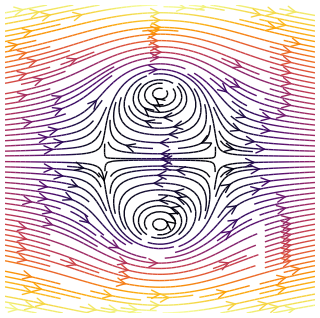
\includegraphics[width=0.3\textwidth,angle=270]{image/Rising_def_Stokes.png}};
        \node (img2) at (0.3\textwidth,0) {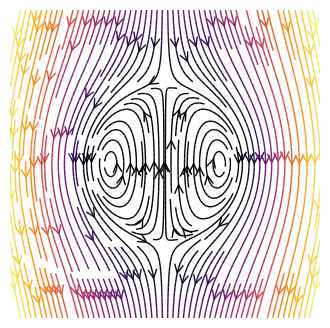
\includegraphics[width=0.3\textwidth]{image/Rising_Stokes.png}};
        % \draw (0.45\textwidth,0)node{$\rightarrow$};
        % \draw (0.45\textwidth,0.4cm)node{$\bm\Gamma_\alpha\cdot \textbf{r}$};
        \node (img1) at (0.0\textwidth,0) {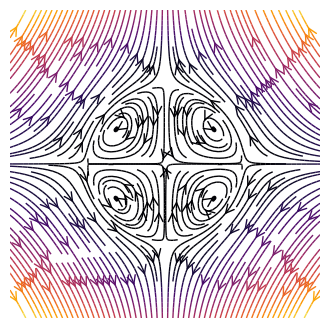
\includegraphics[width=0.3\textwidth]{image/Shear_Stokes.png}};
        % \draw (img3.south)node{(c)};
        \draw (img2.south)node{(b)};
        \draw (img1.south)node{(a)};
    \end{tikzpicture}
    \caption{Examples of steady state flow lines plots of an isolated droplet immersed into a viscous fluid. 
    (a) Rising sphere in uniform stokes flow. 
    (b) Fixed droplet in a pure extensional.
    (analytical solution in \ref{ap:solution_singularity})
    These solutions correspond exactly to the fields $\textbf{u}_f^1$ at order $\mathcal{O}(\phi_d)$.}
    % (c) Deformed droplet in rising motion (analytical solution of \citet{taylor1964deformation}). }
    \label{fig:flowlines}
\end{figure}

We recall that all along this section we consider spherical droplet of radius $a$ with viscosity ratio $\lambda = \mu_d /\mu_f$ and density ratio $\zeta =\rho_d /\rho_f$. 

\subsection{Moment of force traction}

Let us present the closures for the momentum exchange term present in of \ref{eq:dt_hybrid_rhou_f} for dilute suspension of spherical droplets. 
% Specifically, we consider an isolated spherical non-rotating droplet of viscosity $\lambda \mu_f$ immersed in an arbitrary linear flow. 
% Most of the term present in \ref{eq:dt_hybrid_rhou_f} are discussed in\ref{ap:two-fluid_model}, thus let focus on the three exchangek terms.  
It is found that the first three moment of the hydrodynamic forces are related to the mean fluid phase velocity field as, 
\begin{align}
    \label{eq:zeroth_mom}
    \pSavg{\bm{\sigma}_f^0\cdot \textbf{n}_d} &= 
    \phi_d \div\bm\Sigma_f
    + \frac{3\phi_d\mu_f}{2 a^2} 
    \left(\frac{3\lambda+2}{\lambda+1}\right) \textbf{u}_{f p} 
    + \frac{3\phi_d\mu_f}{4} \left(\frac{\lambda}{\lambda+1}\right)\grad^2\textbf{u}_f\\
    \label{eq:first_mom}
    \pavg{\intS{\textbf{r}\bm{\sigma}_f^0 \cdot \textbf{n}_d}} 
    &= 
    \phi_d \bm\Sigma_f + 
    \frac{3}{5}\mu_f \phi_d \left(\frac{2+5\lambda}{1+\lambda}\right)
    \textbf{E}_f
    \\
    \label{eq:second_mom}
        \pavg{\intS{(\bm{\sigma}_f^0 \cdot \textbf{n}_d)_ir_kr_l}} &=
        % \phi_d  \frac{a^2}{5} 3 [(\div \bm\Sigma_f)\bm\delta]^\text{sym}
        + \frac{3\mu_f\phi_d}{2}\left(\frac{\lambda}{\lambda+1}\right)(\textbf{u}_{fp})_i\delta_{kl}\\
        &+ \frac{3\mu_f\phi_d}{5}\left(\frac{1}{\lambda+1}\right)((\textbf{u}_{fp})_i\delta_{kl}+ (\textbf{u}_{fp})_k\delta_{il}+(\textbf{u}_{fp})_l\delta_{ki})\nonumber
\end{align}
where we recall that $\textbf{u}_{fp} = \textbf{u}_f - \textbf{u}_p$, $\bm\Sigma_f = -p_f\bm\delta +2 \mu_f \textbf{E}_f$, and $\textbf{E}_f = \frac{1}{2}\left[\grad \textbf{u}_f + (\grad \textbf{u}_f)^\dagger\right]$. 
Notice that at first order in $\phi_d$, $\phi_d\textbf{u}_f =\phi_d\textbf{u} - \phi_d^2 \textbf{u}_d = \phi_d\textbf{u}$, so one can either use $\textbf{u}_f$ or $\textbf{u}$ in the above definition of $\textbf{u}_{fp}$. 
The term $\pSavg{\bm{\sigma}_f^0 \cdot \textbf{n}_d}$ represents the total components of the interphase drag force.
Specifically, the first term is the mean Newtonian continuous phase stress $\bm\Sigma_f$, the second term is the Hadamard-Rybczynski force and the last is the Faxen contribution \citep{kim2013microhydrodynamics}. 
Likewise, $\pSavg{\textbf{r}\bm{\sigma}_f^0 \cdot \textbf{n}_d}$ is the averaged first moment of the surface force traction, which includes the mean fluid phase stress. 
This tensor is responsible for the well-known Einstein correction to the viscosity (see next section), but here it is adapted to spherical droplets instead of spherical solid particles \citep{rallison1978note}. 
% Therefore, this term is of upmost importance in the averaged momentum equations and is non-negligible in most of the flow conditions, if not all of them.
The second moment of the force traction is made of three contribution, the first one is related to the divergence of the mean fluid phase stress, see \ref{eq:second_mom_general}. 
However, this contribution is negligible at $\mathcal{O}(\phi_d)$ \citep{jackson1997locally} and therefor not shown in \ref{eq:second_mom}.  
The second contribution is proportional to the relative velocity $\textbf{u}_{fp}$.
This was firstly discovered by \citet{nozieres1987local} based on phenomenological arguments and by \citet{lhuillier1992volume} based on theoretical ground, both for spherical solid particles. 
According to the cited author this term induce a coupling between relative motion and convection. 
The second moment of the hydrodynamic forces is non-negligible at first order in $\phi_d$, in agreement with \citep{jackson1997locally,zhang1997momentum}. 
Thus, the zeroth, first and second moment of the drag are non-negligible in the Stokes regime and at $\mathcal(\phi_d)$. 
In \citet{zhang1997momentum} they even stipulated that the third order moment of the force traction is not necessarily negligible at $\mathcal{O}(\phi_d)$ when considering non-spherical particles in stokes flows. 

Consequently, in the stokes and dilute hypothesis, the zeroth, first and third moments of surface traction are non-negligible and are primordial in the modeling of the fluid phase momentum equations. 
It is therefore reasonable that these terms are also relevant for broader flows regime. 
For example, in \ref{chap:deformable} we demonstrate that \ref{eq:first_mom} has a component proportional to the mean phase velocity $\textbf{u}_{fp}\textbf{u}_{fp}$ in the inertial regime. 
Thus, it is surprising that most studies in the literature do not mention the first and second-order moments, which are almost always neglected

\subsection{Pseudo turbulent stress}

Another contribution to the stress is the pseudo-turbulent tensor $\avg{\chi_f \textbf{u}_f'\textbf{u}_f'}$. 
Note that in stokes regime this term is more likely to be negligible, nevertheless it is still interesting to provide its closure based on the Stokes solution as it gives the first order inertial contribution, which is of course non-negligible at finite particle Reynolds number.

In \ref{ap:solution_singularity} we compute this closure based on \ref{eq:Batchelor2}, following the rigorous methodology presented in the previous section.  
The methodology is as follows:
In the Stokes regime $\textbf{u}_f'$ is proportional to $\textbf{u}_{fp}$ and $\textbf{E}_f$. 
Since, $\avg{\chi_f \textbf{u}_f'\textbf{u}_f'}$ is a symmetric second order tensor, the final closure must remain symmetric and second order.
Additionally, the only possible combination of tensor, $\textbf{u}_{fp}$ and $\textbf{E}_f$, which can form a symmetric second order tensor are, 
\begin{align}
    \textbf{u}_{fp}
    \textbf{u}_{fp}
    &&
    \textbf{E}_f\cdot \textbf{E}_f
    && 
    \frac{1}{2}(\textbf{E}_f\cdot \textbf{u}_{fp} \textbf{u}_{fp})
\end{align}
and the unit tensor $\bm\delta$. 
Consequently, we conclude that the functional form of $\avg{\chi_f \rho_f \textbf{u}_f' \textbf{u}_f'}$ must be , 
\begin{multline}
     \avg{\chi_f \rho_f \textbf{u}_f' \textbf{u}_f'}
     =
     C_{uu}^1 \textbf{u}_{fp} \textbf{u}_{fp}
     + C_{EE}^1 \textbf{E}_f\cdot \textbf{E}_f
     + C_{uE}^1 \frac{1}{2}\left(\textbf{E}_f\cdot \textbf{u}_{fp} \textbf{u}_{fp}+ \textbf{u}_{fp} \textbf{u}_{fp}\cdot \textbf{E}_f\right) \\
     + \left[ 
         C_{uu}^2 (\textbf{u}_{fp}\cdot  \textbf{u}_{fp})
         +  C_{EE}^2 (\textbf{E}_f : \textbf{E}_f)
        +  C_{uE}^2 ( \textbf{u}_{fp}\cdot \textbf{E}_f\cdot \textbf{u}_{fp})
    \right]\bm\delta
    \label{eq:Reynolds_stress_functional_form}
\end{multline}
where $C_{uu}^1,C_{EE}^1,C_{uE}^1,C_{uu}^2,C_{EE}^2$ and $C_{uE}^2$ are yet unknown scalar function. 
Note that the term on the second lines represents the isotropic part of the Reynolds stress tensor  which is the pseudo-turbulent energy, $k_f$. 
Physically \ref{eq:Reynolds_stress_functional_form} means that droplets in a flow, induces pseudo turbulence through they relative linear motion, i.e. which is exactly the wake on \ref{fig:flowlines} (left), and the wake when mean linear motions acts around the droplets, see  \ref{fig:flowlines} (right). 

The disturbance fields of a droplet in translation is proportional to $r^{-1}$ thus the computation of the integral of $\avg{\chi_f \rho_f \textbf{u}_f' \textbf{u}_f'}$ in the case of translation diverges if we use \ref{eq:Batchelor2}.
As mentioned in the previous section, (see also \ref{chap:pseudoturbulence}), this divergence issue arise because \ref{eq:Batchelor2} is unable to provide physical results in this regime. 
Nevertheless, since the disturbance field of a droplet in translation is proportional to the relative velocity $\textbf{u}_{fp}$ the functional form of this tensor cannot be otherwise that proportional to $\textbf{u}_{fp} \textbf{u}_{fp}$ and $(\textbf{u}_{fp}\cdot \textbf{u}_{fp})\bm\delta$.
To support that hypothesis, note that for spherical bubbles in potential flow, the pseudo turbulent tensor have the same functional form as the second line of \ref{eq:Reynolds_stress1} (see equation (5.7) of \citet{zhang1994ensemble}). 
Additionally, for ordered array of spheres immersed in a uniform non-inertial flow we found $C_1(\phi) \sim \phi^{2/3}$ \citet{hill2001first}.
It is therefore reasonable to expect the same trend for random array, since in the dilute regime both random and ordered array are supposed to be equivalent. 
Consequently, at this stage we suppose that \ref{eq:Reynolds_stress1} 


Since $\avg{\chi_f \rho_f \textbf{u}_f' \textbf{u}_f'}$ is a symmetric second order tensor with independent components is can be computed with at least $6$ scalar integral. 




\begin{multline}
    \avg{\chi_f \rho_f \textbf{u}_f' \textbf{u}_f'}
    =
    \frac{\phi_d a^2 \rho_f}{105 (\lambda +1)^2 }\left[
        (129\lambda^2+108\lambda+24)\textbf{E}_f\cdot \textbf{E}_f
        + (20\lambda^2 +20\lambda + 6)
        (\textbf{E}_f : \textbf{E}_f)\bm\delta
    \right]\\
    + C_1(\phi,\lambda) [\textbf{u}_{fp} \textbf{u}_{fp}
    + \pavg{\textbf{u}_\alpha'\textbf{u}_\alpha'} ]
    + C_2(\phi,\lambda) [\textbf{u}_{fp}\cdot \textbf{u}_{fp} + 2 n_p k_p]\bm\delta
    \label{eq:Reynolds_stress1}
\end{multline}
Where $C_1$ and $C_2$ are yet unknown constant.
Indeed, 


A droplet immersed in a linear flow also produce pseudo-turbulence. 
The contribution from the mean shear flow to the pseudo turbulent tensor is also derived in \ref{ap:solution_singularity} and reads as the first line of \ref{eq:Reynolds_stress1}. 
In  \citet{raja2010inertial} they study theoretically the stress in a neutrally buoyant suspensions of droplets. 
In the dilute limit they compute the deviatoric part of $\avg{\chi_f \rho_f \textbf{u}_f' \textbf{u}_f'}$ based on the stokes flow solution. 
It is observed that the first term on the right-hand side of \ref{eq:Reynolds_stress1} is consistent with equation (3.15) of \citet{raja2010inertial}.
Regarding the second term of \ref{eq:Reynolds_stress1} it corresponds to the  isotropic contribution of the Reynolds stress.
This term seems new  

finally

\subsection{The fluid phase equivalent stress}
% In this section we focus on the formulation of the averaged fluid phase equivalent stress tensor $\bm{\sigma}_f^\text{Re}$. 
For instance the stress appearing on the left hands side of the fluid phase momentum balance is of the form of \ref{eq:sigma_eq_def}. 
It is more convenient to express the equivalent stress as a Newtonian stress, plus a contribution arising due to the presence of the particles. 
Thus, we reformulate $\bm{\sigma}_f$ considering that $\phi_f \bm{\sigma}_f = - \phi_f p_f + 2 \phi_f \mu_f \textbf{e}_f$ where $2 \phi_f \bm{e}_f = \avg{\chi_f  (\grad \textbf{u}_f^0 + (\grad \textbf{u}_f^0)^T)}$. 
Additionally, we state that the fluid strain is equal to the bulk strain $2\textbf{e} = \grad \textbf{u}+ (\grad \textbf{u})^T$, minus the particle averaged strain, i.e. $\phi_f \mu_f \textbf{e}_f = \mu_f\textbf{e} - \mu_f \phi_d \textbf{e}_d$ which gives
\begin{equation*}
    \bm\sigma_f\phi_f =-\phi_f p_f \bm\delta + 2 \mu_f \textbf{e} -2\phi_d \mu_f \textbf{e}_d.
    \label{eq:def_sigma_f}
\end{equation*}
Under this form we clearly remark that for solid particle $\phi_d \textbf{e}_d = 0$ thus we recover equations (44) of \citet{jackson1997locally} which reads in our notation : $\bm\sigma_f\phi_f =-\phi_f p_f \bm\delta + 2 \mu_f \textbf{e}$. 
Upon developing $\phi_d \textbf{e}_d$ multipolar series using \ref{eq:f_exp}, the equivalent stress of the fluid phase can be reformulated as, 
\begin{multline}
    \bm{\sigma}^\text{eq}_f = 
    \phi_f p_f \bm\delta 
    - 2\mu_f \textbf{e} 
    +\avg{\rho_f\chi_f\textbf{u}_f'\textbf{u}_f'} 
    + 2 \mu_f \pOavg{\textbf{e}_d^0}
    - \pSavg{\textbf{r}\bm{\sigma}_f^0\cdot \textbf{n}_d}
    \\
    + \div \left[
        \frac{1}{2} \pSavg{\textbf{rr}\bm{\sigma}_f^0\cdot \textbf{n}_d}
        - 2 \mu_f\pOavg{ \textbf{re}_d^0 }
        + \ldots
    \right]
    \label{eq:sigma_eq_0}
\end{multline} 
It is worth noting that $\textbf{e} = \grad \textbf{u} + (\grad \textbf{u})^\dagger$. 

Nevertheless, the bulk velocity \textbf{u} is not part of our unknown instead we solve for $\textbf{u}_f$, $\textbf{u}_p$, $\textbf{P}_p$ and eventually the higher moments. 
Therefore, in all rigor we must write 
\begin{equation}
    \textbf{e}
    = 
    \grad \textbf{U} + (\grad \textbf{U})^\dagger
    - \grad (\div (n_p \textbf{P}_p))
    - (\grad \div (n_p \textbf{P}_p))^\dagger
    + \ldots
    \label{eq:rate_of_strain}
\end{equation}
where $\textbf{U} = \phi_f \textbf{u}_f + n_p v_p \textbf{u}_p$ is equivalent to the bulk velocity \textbf{u} uniquely in an homogeneous medium. 

% The fluid phase averaged stress is therefore composed of : 
% (1) the pseudo turbulent contribution $\rho_f\avg{\chi_f  \textbf{u}_f' \textbf{u}_f'}$ which can be decomposed in an isotropic part $2 k_f = \avg{\chi_f \rho_f \textbf{u}_f' \textbf{u}_f'}:\bm\delta$ that contribute to the effective pressure, and a deviatoric part defined as $\avg{\chi_f \rho_f \textbf{u}_f' \textbf{u}_f'} - 2 k_f\bm\delta$. 
% (2) the shear stress $2\mu_f \textbf{e}$ of the fluid phase \ref{eq:rate_of_strain}. 
% (3) the particles internal shear $2\mu_f \pOavg{\textbf{e}_d^0}$
% (4) the particle first moment of the hydrodynamic forces $\pSavg{\textbf{r}\bm{\sigma}_f^0\cdot \textbf{n}_d}$. 
% (5) and the higher order moments of forces and internal shear.  

At this point if one want to write the fluid phase averaged stress as an equivalent Newtonian stress with effective pressure $p^{eff}$ and effective viscosity $\mu^{eff}$ he needs to express each of the closure terms mentioned above as a function of isotropic tensor which will contribute to the effective pressure, or as a linear function of  $\textbf{e}$ which will contribute to the effective viscosity. 
Note that this is not always possible, indeed, according to \ref{eq:second_mom} the second order moment of the hydrodynamic stress is a function of the relative velocity and not of the mean shear rate. 
Thus, in addition to the Newtonian behavior of the averaged fluid one must be prepared to find non-Newtonian terms purely related to the dispersed nature of the flow. 

Once again it is useful to consider the stokes flow regime to provide a closed form of the fluid phase stresses. 
To that end notice that the internal shear rate inside the particles minus the external fluid traction for isolated spherical droplets in an arbitrary linear flow can be written, 
% \begin{align}
%     \pOavg{\textbf{e}_d^0}
%     = 
%     \phi_d 
%     \textbf{E}_f
%     \frac{3}{5}\frac{1}{\lambda+1}
%     \\
%     \pOavg{\mu_f \textbf{e}_d^0\textbf{r} }
%     = 
%     - \frac{\phi_d\mu_f}{10(\lambda+1)}
%     \left[
%         (\bm\delta \textbf{u}_{fp})_{ijk}
%         - \frac{3}{2}
%         \left[
%             (\bm\delta \textbf{u}_{fp})_{kij}
%             + (\bm\delta \textbf{u}_{fp})_{jki}
%         \right]
%     \right]
%     \label{eq:closur_e}
% \end{align}
% Notice that the second moment of momentum is present under the $\partial_k\partial_l$ operator in the moment of momentum equation, meaning that the skew-symmetic part of $\pavg{\intS{(\bm{\sigma}_f^0 \cdot \textbf{n}_d)_ir_kr_l}} $ and $\pSavg{{\mu(\textbf{e}_d^0)_{ik} r_l}}$ vanish in the momentum equation. 
% Therefore, the second moment of surface traction force might be written, 
\begin{align*}
    \pavg{\intS{(\bm{\sigma}_f^0 \cdot \textbf{n}_d)_ir_k}} -
    2\pSavg{{\mu(\textbf{e}_d^0)_{ik}}} 
    &= 
    \phi_d p_f\bm\delta
    - \frac{5\lambda +2}{\lambda +1}
    \textbf{e}_f \phi \mu_f
    \\
    \frac{1}{2}\pavg{\intS{(\bm{\sigma}_f^0 \cdot \textbf{n}_d)_ir_kr_l}} -
    2\pSavg{{\mu(\textbf{e}_d^0)_{ik} r_l}} 
    &= 
    \frac{\mu_f\phi_d}{2(\lambda +1) }
    \left[
        \frac{3\lambda}{2} 
        u_{fp,i}\delta_{kl}
        +  u_{fp,l}\delta_{ki}
    \right]. 
\end{align*}
Considering this relation together with \ref{eq:sigma_eq_0}, \ref{eq:second_mom} and \ref{eq:first_mom} we can re-write the effective stress of the suspension as, 
\begin{multline}
    \bm{\sigma}^\text{eq}_{f,ik} =
    + \rho_f\avg{\chi_f\textbf{u}_f'\textbf{u}_f'}_{ik} 
    + p_f \bm\delta
    - 2 \mu_f \textbf{e}\left[
        1
        +\frac{\phi_d}{2}\left(
            \frac{5\lambda +2}{\lambda +1}
        \right)
    \right]\\
    + 
    \frac{\mu_f 3\lambda}{4(\lambda +1) }
    \left[
        \grad (\phi_d\textbf{u}_{fp,i})
        +  
        \frac{2}{3\lambda} 
        [\div (\phi_d\textbf{u}_{fp,l})]\bm\delta_{ki}
    \right]
\end{multline} 
This expression is in agreement with \citet[Appendix A]{zhang1997momentum}. 
In order to highlight that the stress tensor is symmetric we add and remove the term $ \grad \textbf{u}_{fp,i}^\dagger$  to the stress and notice that only the symmetric part in the indices $kl$ remain under the application of the double gradient operator present in the momentum equation. 
Based on similar arguments than \ref{eq:sym_proof} we can show that it gives, 
\begin{multline}
    \bm{\sigma}^\text{eq}_{f,ik} =
    + \rho_f\avg{\chi_f\textbf{u}_f'\textbf{u}_f'}_{ik} 
    + p_f \bm\delta
    - 2\mu^\text{eff} \textbf{e}
    + \\
    \mu_\text{U}^\text{eff}
    \left[
        \partial_k   (\phi_d\textbf{u}_{fp,i})
        + \partial_i (\phi_d\textbf{u}_{fp,k})
        + \frac{2-3\lambda}{3\lambda}  [\div (\phi_d\textbf{u}_{fp,l})]\bm\delta_{ki}
    \right]
    \label{eq:fluid_phase_stress}
\end{multline} 
The equivalent viscosity of the fluid are given by 
\begin{align*}
    \mu^\text{eff} = \mu_f \left[
        1
        +\frac{\phi_d}{2}\left(
            \frac{5\lambda +2}{\lambda +1}
        \right)
    \right] &&
    \mu^\text{eff}_\text{U}
    = \mu_f\frac{ 3\lambda}{4(\lambda +1) }
\end{align*}
Thus, in linear dilute stokes flow the equivalent stress is not Newtonian since it has an additional contribution arising from the relative phase velocity appears. 
Additionally, we can predict that the term $\rho_f\avg{\chi_f\textbf{u}_f'\textbf{u}_f'}$ will induce non-Newtonian behavior as well as an effective pressure contribution. 

\subsection{Energy exchange terms}


Now let us focus on the last term of \ref{eq:exergysource}.
As mentioned above this term represents the source of pseudo turbulent energy in the fluid phase due to the presence of the particles. 
As a first approximation one might consider that in average a particle in the flow posses the surface velocity of an isolated particle in an arbitrary linear flow stokes flow with relative velocity  $\textbf{u}_{fp}$ and mean shear $\textbf{E}_f$.
In this case the \textit{inner velocity} evaluated at the surface of the particle $\alpha$ can be written as (see \ref{ap:Closure_problem})
% \begin{equation*}
%     \textbf{w}_d^0 (\textbf{x}_\alpha + \textbf{r})
%     = \left(\frac{\lambda + \frac{1}{2}}{\lambda +1} - 1\right)
%     (\textbf{u}_{f} - \textbf{u}_\alpha) 
%     + 
%     \frac{1}{2a^2}\left(\frac{1}{\lambda +1}\right)
%     \textbf{rr} \cdot (\textbf{u}_{f} - \textbf{u}_\alpha) 
%     + \left[1-\frac{\lambda}{(\lambda + 1)}\right]\textbf{E}_f\cdot\textbf{r}
%     -\frac{1}{a^2}\left(\frac{1}{\lambda +1 } \right) \textbf{r} \textbf{E}_f:\textbf{rr}. 
% \end{equation*}
\begin{equation*}
    \textbf{w}_d^0 (\textbf{x}_\alpha + \textbf{r})
    = 
    \frac{1}{\lambda +1} \left[\left(
        -\frac{\bm\delta}{2}
        + 
        \frac{\textbf{rr}}{2a^2}
    \right)\cdot (\textbf{u}_{f} - \textbf{u}_\alpha) 
    + \left(\textbf{r}\bm\delta
    -\frac{1}{a^2}\textbf{rrr}\right)\cdot \textbf{E}_f
    \right].
\end{equation*}
The contributions of the velocity field factor of $\textbf{u}_{fp}$ represents the famous hill's vortex reticulation inside a spherical droplet. 
The second contribution is the motion generated due to a mean shear flow. 
Injecting this expression into the Last term on the right-hand side of \ref{eq:exergysource} gives, 
\begin{align}
    \pSavg{\textbf{w}_2^0 \cdot \bm{\sigma}_1^0\cdot\textbf{n}_2}
    &=  
    \frac{1}{\lambda+1}\textbf{u}_{fp} \cdot \left[
        -\frac{1}{2}\pSavg{ \bm{\sigma}_1^0\cdot\textbf{n}_2}
        % + \pavg{\textbf{u}_{\alpha}' \cdot \intS{ \bm{\sigma}_1^0\cdot\textbf{n}_2} }
        + \frac{1}{2a^2}
        \pSavg{\textbf{rr}\cdot \bm{\sigma}_1^0\cdot\textbf{n}_2}
    \right]\nonumber
    \\
    &+ \frac{1}{\lambda+1} \left[
        -\frac{1}{2}
        \pavg{\textbf{u}_\alpha' \cdot  \intS{\bm{\sigma}_1^0\cdot\textbf{n}_2}}
        % + \pavg{\textbf{u}_{\alpha}' \cdot \intS{ \bm{\sigma}_1^0\cdot\textbf{n}_2} }
        + \frac{1}{2a^2}
        \pavg{\textbf{u}_\alpha' \cdot \intS{\textbf{rr}\cdot \bm{\sigma}_1^0\cdot\textbf{n}_2}}
    \right] \nonumber
    \\
    % \left[
    %     \textbf{u}_{p f} \cdot
    %     +
        % \pavg{\textbf{u}_{\alpha}' \cdot \intS{\textbf{rr}\cdot \bm{\sigma}_1^0\cdot\textbf{n}_2}}
    % \right]
    &+ \frac{1}{\lambda + 1} \textbf{E}_{f} : \left[ 
         \pSavg{\textbf{r} \bm{\sigma}_1^0\cdot\textbf{n}_2}
         -\frac{1}{a^2} 
         \pSavg{ \textbf{rrr} \cdot \bm{\sigma}_1^0\cdot\textbf{n}_2}
         \right]
    \label{eq:energy_term}
\end{align}
\tb{maybe explicite those terms and disscus and compare with L. M. Liljegren (1996) for solid particles; say that he neglect all of the first moments }
In this expression we clearly identify the zero, first and second order moments of the surface force traction provided by \ref{eq:first_mom}. 
Additionally, notice that we did not consider rotation of droplets consequently the mean fluid vorticity nor the particles angular velocity appears in this expression. 
One can also notice that taking the limit $\lambda \to \infty$ gives zero for \ref{eq:energy_term}. 
Which is consistent since $\textbf{w}_d^0 = 0$ for non-rotating solid particles. 
Consequently, in light of \ref{eq:energy_term} the work generated due to the local motion at the surface of a spherical droplet, namely  $\pSavg{\textbf{w}_2^0 \cdot \bm{\sigma}_1^0\cdot\textbf{n}_2}$ is either due to its relative motion with the continuous phase  or due to its simple presence in a shear flow. 
Indeed, in both cases motion at the surface of the particle is observed and stresses is also generated, which in turns contribute the generation of pseudo turbulence. 
In fact if we add the contribution given by \ref{eq:energy_term} in  \ref{eq:dt_hybrid_k1} we observe that  the consideration of hill's vortexes add the coefficient $\frac{\lambda +\frac{1}{2}}{\lambda+1}$ in front of the drag force velocity terms in \ref{eq:dt_hybrid_k1}.
Besides, the first moments of surface traction forces appearing in the diffusive equivalent flux $\textbf{q}_1^k$ are also subject to these comments.  
Consequently, the consideration of hill's vortex end up to add a coefficient in front of this exchange term which varies from $1$ to $1/2$ for respectively, solid particles and bubbles.  
Same comments can be made regarding the consideration of the droplets internal motion to the higher moments present in the flux term $\textbf{q}^k_f$. 

As a matter of fact the consideration of the internal motion of particles such as hill's vortex have a very significant impact regarding the magnitude of the pseudo turbulent exchange terms, especially when one is considering bubbly flow. 
The physical explanation of the decrease of the coefficient in front of the exchange terms for bubbles, can be due to the facts that the fluid slip on the bubbles or droplet's surface induce less work exchange than if the fluid followed the particle's surface as it is the case for solid particles. 

\subsection{Particles induced dissipation}

Another closure of upmost importance in the pseudo turbulent equation is the fluid phase dissipation $\avg{\chi_f \bm\sigma_f^0 :\grad\textbf{u}_f^0}$. 
Here we propose to compute this term based on the stokes flow solution given in \ref{ap:Closure_problem}. 
Thus, we only consider here, what we call the \textit{particle induced dissipation}.
This means that we consider only the dissipation in the fluid phase that is due to particle relative motions. 
This reads, 
\begin{multline}
    \avg{\chi_f \bm\sigma_f^0 :\grad\textbf{u}_f^0}
    =
    \frac{3\mu_f \phi_d}{2a^2}
    \frac{(3\lambda^2 + 4\lambda +2)}{(\lambda + 1)^2}
    (\textbf{u}_{fp}\cdot \textbf{u}_{fp} + 2 k_p ) \\
    + 
    \frac{3\mu_f \phi_d}{5}
    \frac{(5\lambda^2 + 4\lambda +4)}{(\lambda + 1)^2}
    \textbf{E}_f:\textbf{E}_f
    +2 \phi_f \textbf{E}_f:\textbf{E}_f
\end{multline}
We can observe that the first two terms are related to the particle relative translation with the continuous phase. 
The second term is the contribution to the fluid phase dissipation due to the  disturbance field of particle in linear flow. 
To the authors' knowledge this closure term is original and must be used as a theoretical ground to extend closure in other regime. 
\tb{notice that the term in factor of the relative vel is the drag}


The remaining closures in the equation of $k_p$, i.e. $\rho_f \avg{\chi_f \textbf{u}_f' k_f}$ and $\avg{\chi_f \textbf{u}_f' \cdot \bm{\sigma}_f^0}$, are in fact null in stokes flow. 
This is because these terms are by nature produced due to the asymmetry of the disturbance fields. 

\tb{ajouter les termes croisées}

\subsection{Internal kinetic energy and dissipation}
% Most of the closure terms present in these expressions also appear in the continuous phase. 
% They have therefore already been discussed. 
Now we discus the term appearing on the right-hand side of \ref{eq:dt_hybrid_Wp} which appears only in the particle-phase equations. 
It is interesting to mention that in the context of unreformable sphere in stokes flows the internal energy term as well as the internal dissipation can in fact be computed directly in terms of the continuous phase unknowns. 
The details of the calculation is given in \ref{ap:Closure_problem} the result yields, 
\begin{align}
    \label{eq:stokes_Wp}
    W_p =  \frac{\rho_d \phi_d}{24 (\lambda +1)^2}
    (\textbf{u}_{fp} \cdot \textbf{u}_{fp} + 2 k_p)
    + \frac{a^2 \rho_d \phi_d}{30(\lambda+1)^2}
    \textbf{E}_f:\textbf{E}_f    \\
    \pOavg{\bm{\sigma}_2^0:\grad \textbf{u}_2^0}
    % = 2\mu_2 \intO{\textbf{e}_2^0: \textbf{e}_2^0 }
    = 
    \frac{6 \phi_d \mu_f \lambda}{a^2(1+\lambda)^2}
    (\textbf{u}_{fp}\cdot \textbf{u}_{fp} + 2k_p)
    + \frac{3 \phi_d \mu_f \lambda}{(\lambda+1)^2}\textbf{E}_f:\textbf{E}_f
    \label{eq:diff_d}
\end{align}
From \ref{eq:stokes_Wp} we deduce that the relative motion between phases $\textbf{u}_{pf}$, as well as the mean gradient of the flow $\textbf{E}_f$ induce an inner circulation inside the droplets. 
As can be seen under this hypothesis the internal energy is not an unknown anymore, since it is entirely determined by the fluid phase unknown and $\phi_d$. 
Nevertheless, it is still non-zero at finite Reynolds number and therefor it must be considered in \ref{eq:E_p_def}. 
The dissipation term given by \ref{eq:diff_d} represents the energy dissipated into heat inside the particles. 
Due to the finite value of $\mu_d$ this term remains non-null. 
Since the motion inside the particles is directly determined by $\textbf{u}_{pf}$ and $\textbf{E}_f$ the dissipation rate equally. 

\tb{Ajouter les terms croisées}

\subsection{Second moment equations closure}

The second moments equations describe the shape and the rate of deformation of the particles.
In this section we assumed implicitly that the droplets remain spherical due to the low capillary number considered. 
Therefore, \ref{eq:dt_hybrid_Mp} and the deviatoric part of \ref{eq:dt_hybrid_Sp} is of no use. 
Moreover, we didn't consider rotation of the particles as well thus \ref{eq:dt_hybrid_mup} cannot be discussed further. 
Nevertheless, computing the closure terms present in of these equations for spherical droplets still gives us hints of their physical significance that their would have if deformation where considered.
Therefore, for pedagogical purposes we now discuss the terms present in \ref{eq:dt_hybrid_Sp} for droplets in an arbitrary linear flow. 


A droplet in an arbitrary linear stokes flow remains spherical at low capillary number due to the competitive contribution of the drop internal stress, the interfacial stress and the surface tension, namely, 
\begin{align*}
    \intO{\bm{\sigma}_d^0},
    &&\frac{1}{2}\intS{(\textbf{r}\bm\sigma_f^0+\bm\sigma_f^0\textbf{r})\cdot \textbf{n}},
    &&\intS{\gamma(\bm\delta - \textbf{nn})},
\end{align*}
respectively. 
The contribution from the continuous phase stress is given by \ref{eq:first_mom}, the particle internal stress can be computed directly from the singularity solution and reads, 
\begin{equation*}
    \pOavg{\bm{\sigma}_d}
    = \frac{6}{5}\phi \mu_f \frac{1}{1+\lambda} \textbf{E}_f
\end{equation*}
From  \ref{eq:Batchelor} we deduce that, 
\begin{equation*}
    \pSavg{\gamma(\bm\delta - \textbf{nn})}
    = 
    \frac{1}{2}\pSavg{(\textbf{r}\bm\sigma_f^0+\bm\sigma_f^0\textbf{r})\cdot \textbf{n}},
    - \pOavg{\bm{\sigma}_d^0},
\end{equation*}
Indeed, as the singularity solution for a droplet is pur linear flow is obtained in the asymptomatic limit of small deformation the surface tension tensor cannot be computed based on the geometrical consideration in which case this contribution would be isotrope leaving the system unbalanced.

The spherical shape equilibrium is valid in the stokes flow regime. 
Now what if little inertial effects where to come into account  ?
Indeed, it is interesting to compute the form of the inertial term appearing in \ref{eq:dt_hybrid_Sp} to evaluate the influence of small inertial effects on the particle shape. 
At the first order in Reynolds number the inertial terms can be computed based on stokes flow solution. 
Therefore, based on the singularity solution of stokes flow we obtain, 
\begin{align*}
    \pOavg{\rho_d \textbf{w}_d^0  \textbf{w}_d^0 }
    &= \frac{\rho_d \phi_d}{140(\lambda +1 )}
    \left[
        7\textbf{u}_{fp}\textbf{u}_{pf} 
    + (\textbf{u}_{pf}\cdot \textbf{u}_{pf})\bm\delta
    + 7\pavg{\textbf{u}_\alpha'\textbf{u}_\alpha'}/n_p 
    + 2k_p \bm\delta
    \right]\\
    &+ \frac{\rho_d \phi_d a^2}{315 (\lambda + 1)^2}[(\textbf{E}_f : \textbf{E}_f)\bm\delta+15\textbf{E}_f\cdot \textbf{E}_f]
    \label{eq:ww_closure}
\end{align*}
This term represents the contribution form the inertial motion within the droplet to the shape of the particle. 
We can observe that relative velocity $\textbf{u}_{fp}$ plays a role in the stretching of momentum balance. 
Therefore, we can state here that the inertia contribution of this term in the stretching of momentum balance \ref{eq:dt_hybrid_Sp} induce a coupling between droplets translation and deformation. 
Of course, this term is only useful in the context were the first order correction in the Reynolds number are considered for all closure. 
Nevertheless, this is beyon the scope of this study nevertheless note that in light of \ref{eq:ww_closure} it is reasonable to expect that the stresslet term as well as the particle internal stress might be $\sim \textbf{u}_{fp}\textbf{u}_{pf} $ as well. 



\section{Discussion and conclusion}
We provided a well-developed hybrid model for dispersed two phase flow made of \ref{eq:avg_dt_chi_f} for the continuous phase, and the moment equations \ref{eq:avg_dt_dq_alpha_tot} and \ref{eq:avg_dt_dQ_alpha_tot} for the particle phase. 
It is derived in the most general way based on volume and surface governing equations valid at the local scale, namely \ref{eq:dt_f_I} and \ref{eq:dt_f_k}. 
After averaging the equations that govern the dispersed phase using two distinct frameworks, namely, the phase-averaged and particle-averaged equations, we demonstrated the equivalence between both formalism by carrying out a series expansion. 
In light of \ref{eq:scheme_equivalence} we reached the major conclusion of that work, i.e.  the phase-averaged equation for the dispersed phase, is a series expansion of the particle averaged equations.  
As assumed by \citet{zhang1997momentum} it is possible to describe a particle with an arbitrary order of accuracy by deriving the moments equations of a particle. 
In this work we provided a general form of these equations together with a clear physical explanation. 
Acknowledging this fact we concluded that  any physical phenomenon could be modeled with the moments equations since they constitute the phase-averaged equation, i.e. \ref{eq:avg_dt_chi_f} for $k =2$. 
Overall, the main advancement of this model is its ability to incorporate the effects of the particles' surface and volume properties, and provide a framework for deriving particle-average equations tailored to any type of problem.
In addition, to the first order conservation laws we also derived the higher order moments equations. 

To illustrate our point all along the derivation of the hybrid model we treat the case of the momentum conservation equation. 
It is shown that the surface tension play no role on the linear and angular momentum, but it does  affect so-called stretching of momentum of a particle. 
In general any surface diffusive flux are not involved in the linear moment\ref{eq:avg_dt_dq_alpha_tot} but play as a source term in the first order moment balance equations. 

To give a more physical insight on these moments equations we end thie work by proposing some examples. 
First we showed and discus how from these moments equations we can find back already demonstrated laws, such as the Rayleigh-Pesslet equations or the orientation tensor equation in fiber suspension. 
Then, we propose a new case were we use the first moment equation of the surfactant distribution to derive a transport equation of the center of mass of surfactant along the surface of the particle. 

The main draw back of this work is that inter particles interactions are not included naturally in these models. 
It would be interested in a future studies to show how pair particles statistics can be unpacked from the phase-averaged equation. 

\tb{Discus the closure terms}
\tb{Insist on the flexibility of this model, it can be apply to any kind of particle nature, liquid, deformable  solid, solid etc..}
\tb{Do a bullet list conclusion}
\tb{INSIST On the fact that all physial phenom is included in the moments equation. 
This is teh cause of the equivalence priciple}


%%%%%%%%%%%%%%%%%%%%%%%%% CHAPITRE 2
\chapter{Averaged equations for deformable ellipsoidal fluid particles : Stress in homogeneous buoyant rising deformable bubbles suspension }
\localtableofcontents

\section{Introduction}
\label{sec:intro_ellipse}
Many studies have been conducted to determine the influence of the droplets' deformation on suspension Rheology \citet{goddard1967nonlinear,lhuillier1987phenomenology,maffettone1998equation,raja2010inertial}.
Most of the authors if not all of them considered the Rheology of neutrally buoyant droplets in linear flows. 
In fiber media modeling it is common to use averaged equations describing the averaged orientation of fiber in a suspension, for example see \citep{wang2008objective}. 
However, these equations (1) do not consider the particles' deformation, and (2) they neglect inertial contribution. 
In the study by \citet{curtiss1956kinetic}, a set of averaged equations describing the mass and momentum conservation of axisymmetric solid particles was derived including the effect of inertia. 
To the authors' knowledge, since the cited studies, no other extended model for non-isotropic deformable particles has been proposed. 
In this work, we would like to present a more general framework in which we consider the deformation of droplet's in arbitrary linear flows, including relative translation between phases. 
% We would like to generalize this approach including the effect of inertia, deformation as well as buoyancy forces. 

% Therefore, this chapter aims to propose a minimal set of averaged equations describing the mean particle shape and orientation of the particles. 
Therefore, in this chapter we explore the possibility to derive a set of averaged equations describing particle deformation, orientation and the kinematic counterpart of these properties. 
We first describe the behavior of a single deformable drop, and propose a minimal set of conservation laws to describe its orientation and deformation. 
Specifically, we consider deformable ellipsoidal particles, which might represent rising droplets or bubbles under the action of gravity, which are known to adopt an ellipsoidal shape \citep{taylor1964deformation} at low inertial effect.
After a complete presentation of the closure problem, we decide to focus on a simplifying senario. 
More specifically, we present effect of uniform phase relative motion on the Rheology at finite Reynolds number, and how this is closely related to the particle deformation. 



In organization of this chapter is as follows. 
In \ref{sec:local_eq_ellipse} we recall the general form of the Lagrangian equations governing the continuous and dispersed phases bulk quantities as well as the interfaces properties.
Then, in \ref{sec:Lagrange_ellipse} we introduce the Lagrangian conservation equation, describing the evolution of the particle mass, velocity, momentum, second-moment of mass and moment of momentum conservation. 
Then, by assuming, a priori, that the particle adopt an ellipsoidal shape we demonstrate that the equations of deformation and orientation arise naturally from the first moment of momentum and the second-order moment of mass of the particle.
In \ref{sec:averaged_ellipsoid} we expose the set of averaged equation for the particle orientation and deformation. 
It is shown that by expressing the particle's properties in the eigenbasis of the particle second moment of mass, we reduce drastically the number of equations. 
Lastly, in \ref{sec:particle_def} we make use of the averaged equation of deformation to compute the deformation of buoyant droplets in dilute emulsions. 
It is shown that the deformation is cased by the \textit{Stresslet} tensor, which also appears in the equivalent continuous phase stress.
We conclude that the effect of small inertia generates a stress proportional to the square of the relative velocity, which in turns deform the droplets. 


%\section{The two-fluid model}
% \section{Eulerian equation of motion}
\section{Local scale equations}
% \label{sec:two-fluid}
\begin{figure}[h!]
    \centering
    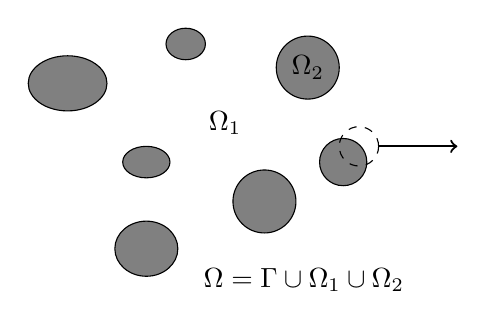
\begin{tikzpicture}
        \foreach \x/\y/\ra/\r in {
        1/3/0.2/0.25,
        2.55/2.7/0.4/0.4,
        0.5/0.4/0.35/0.4,
        2/1/0.4/0.4,
        3/1.5/0.3/0.3,
        0.5/1.5/0.2/0.3,
        -0.5/2.5/0.35/0.5}{
            \draw[fill=gray](\x,\y) ellipse(\r cm and \ra cm);
        }
        \draw[dashed](3.2,1.7)circle(0.25);
        % \draw[thick,->](3.2,1.7)++(0.1767,0.1767)--++(0.4,0.4)--++(1,0);
        \draw[thick,->](3.2,1.7)++(0.25,0)--++(1,0);
        \draw(2.55,2.7)node{$\Omega_2$};
        \draw(1.5,2)node{$\Omega_1$};
        \draw(2.5,0)node{$\Omega = \Gamma \cup \Omega_1 \cup \Omega_2$};
        % \draw(2.5,-1)node{$\Gamma = \sum_\alpha \Gamma_\alpha$};
        % \draw(2.5,-0.5)node{$\Omega_2 = \sum_\alpha \Omega_\alpha$};
    \end{tikzpicture}
    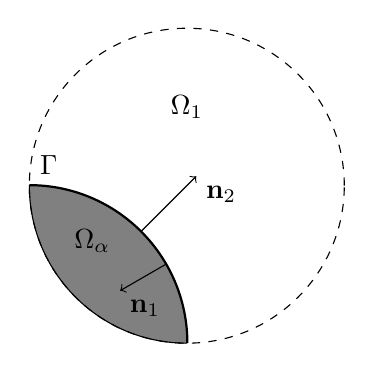
\begin{tikzpicture}%[scale = 0.9]
        \draw[very thick](0:2)arc(0:90:2)node[above right]{$\Gamma$};
        \draw[fill=gray](0:2)arc(0:90:2)arc(180:270:2);
        \draw[dashed](2,2)circle(2);
        \draw[->](1.42,1.42)--++(0.7,0.7)node[below right]{$\textbf{n}_2$};
        \draw[->](1.73,1)--++(-0.577,-0.333)node[below right]{$\textbf{n}_1$};
        \draw(2,3)node{$\Omega_1$};
        \draw(0.8,1.3)node{$\Omega_\alpha$};
    \end{tikzpicture}
    \caption{Domain definitions and scheme of the topology of dispersed two-phase flows.}
    \label{fig:Scheme}
\end{figure}
We consider a system consisting of two phases, separated by a sharp interface $\Gamma(t)$ which evolves over time. 
Each phase subdomain is denoted $\Omega_1(t)$ and $\Omega_2(t)$ for the continuous phase ($1$) and the dispersed phase ($2$) respectively (see \ref{fig:Scheme}). 
The mathematical and physical definition of $\Gamma(t)$ is by no means straightforward, therefore, the interested reader is refereed to \cite{bothe2022sharp} to have a deeper understanding of sharp interface modeling. 
The entire domain, denoted as $\Omega$, is defined as the union of $\Omega_1$, $\Omega_2$, and $\Gamma$.
To track the position of the phase indexed $k$ and the interfaces, we introduce the phase indicator function and the interface indicator function, 
\begin{align}
    \chi_k(\textbf{x},t) =  \left\{
      \begin{tabular}{cc}
        $1 \;\text{if} \;\textbf{x} \in \Omega_k(t)$\\
        $0 \;\text{if} \;\textbf{x} \notin \Omega_k(t)$
      \end{tabular}
      \right.
      \text{for $k = 1,2$},
    %   \label{eq:PIF}
    && \delta_I(\textbf{x},t) =  \left\{
      \begin{tabular}{cc}
        $1 \;\text{if} \;\textbf{x} \in \Gamma(t)$\\
        $0 \;\text{if} \;\textbf{x} \notin \Gamma(t)$
      \end{tabular}
      \right.,
    %   \label{eq:PIF}
\end{align}
respectively. 
For clarity, we omit the time and position arguments of $\chi_k(\textbf{x},t)$ and $\delta_I(\textbf{x},t)$ in the following sections. 

For the purpose of clarity, we only consider the specific case of the mass, momentum and energy conservation equations for a buoyant dispersed two phase flow.
Equally, we consider a constant density and viscosity in each domain as well as a constant surface tension on the interfaces.

% \subsubsection{Inside the volumes}
Within phase $k$, we note $\rho_k$ the density, $\textbf{u}_k^0$ the local velocity and $E_k^0$ the local total energy per units of mass.
All over the domain $\Omega_k(t)$ the mass, momentum and total energy obey these conservation laws :
\begin{align}
    \label{eq:dt_rho}
    \pddt \rho_k  
    + \div (
        \rho_k\textbf{u}_k^0
    )
    &= 
    0\\
    \label{eq:dt_rhou_k}
    \pddt (\rho_k\textbf{u}_k^0)  
    + \div (
        \rho_k\textbf{u}_k^0\textbf{u}_k^0
        - \bm{\sigma}_k^0 
    )
    &= 
    \rho_k \textbf{g}\\
    \label{eq:dt_rhoE_k}
    \pddt (\rho_kE_k^0)  
    + \div (
        \rho_kE_k^0\textbf{u}_k^0
        + \textbf{q}_k^0
        - \textbf{u}_k^0 \cdot \bm{\sigma}_k^0 
        )
    &= 
    \textbf{u}_k^0 \cdot \textbf{g}  \rho_k
\end{align} 
All along this work the continuous phase will be considered as Newtonian fluid thus, $\bm{\sigma}_1^0 = - p_1^0 \textbf{I} + \bm{\tau}_1^0$ where $\bm{\tau}_1^0$ is the Newtonian stress tensor with $p_1 ^0$ the local pressure and $\bm{\tau}_1^0 = \mu_1[\grad \textbf{u}_1^0+(\grad \textbf{u}_1^0)^T]$ the shear rate. 
The vector $\textbf{q}_k^0$ represent the thermal energy flux and is often model with a Fourier law : $\textbf{q}_k^0 = -\lambda \grad T_k^0$ where $T_k$ is the temperature and $\textbf{g}$ is the acceleration of gravity which will be the only body force in the present problem. 
All along this work the superscript $^0$ indicate that the variable is defied at the local or microscopic scale, in opposition to the averaged or macroscopic quantities that will be presented latter. 

% \subsubsection{On interfaces}

On the interfaces the mass, momentum and total energy balance equations reduce to the common expressions :
\begin{align}
    \label{eq:dt_rho_I}
    \textbf{u}_I = \textbf{u}_k
    &=0, \\
    \Jump{\bm{\sigma}_k^0} 
    &=
    \divI\bm\sigma^0_{I||}
    =
    \gamma\kappa\textbf{n},
    % + \gradI\sigma 
    \label{eq:surface_tension}\\
    \label{eq:dt_rhoI_uI2}
    \Jump{\textbf{u}_k^0 \cdot \bm{\sigma}_k^0}
    &=
     \gamma\kappa\textbf{n}\cdot \textbf{u}_{I}^0\\
    \label{eq:dt_rhoIe_I}
    \Jump{ \textbf{q}_k^0}
    &= 
     0
\end{align}
for the interface kinetic energy and the internal interface energy, respectively. 
Notice that this decomposition is possible only under the assumption of no mass transfer in which case $\textbf{u}_I^0=\textbf{u}_k^0$ for $k =1,2$ and a constant surface tension coefficient.



\section{Lagrangian equations for the dispersed phase}
% \label{sec:Lagrangian}

While \ref{eq:dt_chi_k_f_k} and \ref{eq:dt_delta_I_f_I} describe multiphase-flow in a general manner, they do not leverage the topology of the dispersed phase. 
Therefore, in this section, we present a Lagrangian-based model capable of describing the dispersed phase with an arbitrary order of accuracy.

\subsection{Fundamental properties}

At this stage, it is crucial to define some fundamental properties associated to each particle.
Following the strategy of \citet{lhuillier2009rheology,lhuillier1992volume,zaepffel2011modelisation} and \citet[Chapter 2]{morel2015mathematical}
we define the mass, position of center of mass, momentum and total energy of the particle $\alpha$, such as,
\begin{align}
    &m_\alpha(t)
    = \int_{\Omega_\alpha(t)} \rho_2  d\Omega,
    % &&
    &\textbf{x}_\alpha(t)
    = \frac{1}{m_\alpha(t) }\int_{\Omega_\alpha(t)} \rho_2 \textbf{x} d\Omega,\\
    % &&
    &\textbf{p}_\alpha(t) 
    = \int_{\Omega_\alpha(t)} \rho_2 \textbf{u}_2^0 d\Omega,
    % &&
    & m_\alpha E_\alpha(t) 
    = \int_{\Omega_\alpha(t)} \rho_2 [e_2^0 + (u_2^0)^2/2] d\Omega,
    \label{eq:position_and_momentum_def}
\end{align}
respectively. 
Where $\Omega_\alpha$ is the domain occupied by the particle $\alpha$ (see \ref{fig:Scheme}). 
Subsequently, we define the velocity of the particle's center of mass, denoted as $\textbf{u}_\alpha$ which is given by $\textbf{u}_\alpha = \ddt{ \textbf{x}_\alpha}$. 
The derivation of $\ddt {\textbf{x}_\alpha}$ is straightforward but requires some algebra which are detailed in \ref{ap:velocity_definition}. 
The final expression reads,
\begin{equation}
    \textbf{u}_\alpha(t) = \frac{1}{m_\alpha(t)} \left(
        \textbf{p}_\alpha(t)
        +  \int_{\Sigma_\alpha(t)} \rho_2 \textbf{r} (\textbf{u}_I^0 - \textbf{u}_2^0)\cdot \textbf{n}_2 d\Sigma
        \right),
        \label{eq:dt_y_alpha}
\end{equation}
where $\textbf{r}(\textbf{x},t) = \textbf{x} - \textbf{x}_\alpha(t)$. 
In Equation \ref{eq:dt_y_alpha}, it can be observed that the first component of the velocity represents the linear momentum divided by the mass of the particle. 
This corresponds to the mass-averaged velocity over the volume of the particle.
The second term in Equation \ref{eq:dt_y_alpha} arises from the contribution of anisotropic mass transfer across the surface of the particle. 
This mass transfer leads to the motion of the particle's center of mass, thereby contributing to the total velocity.
To illustrate this concept, let us consider a fixed drop with no momentum lying over a very hot plate.
In this scenario, we assume that the plate is sufficiently hot to induce evaporation, specifically on the bottom portion of the drop.
Hence, under the effect of an anisotropic evaporation flux one may expect the second term to be non-negligible.
Consequently, the center of mass of the drop has a non-zero velocity in the opposite direction of the plate, even though the momentum is assumed to be zero.
We can also consider the case of the nucleation of a bubble in water. 
In this case, although the particle momentum is null at all time the center of mass of the particle moves due to the growth of the particle. 
In both cases, we need to take into account the mass transfer term in \ref{eq:dt_y_alpha}, while the first term is negligible. 
Note that \ref{eq:dt_y_alpha} generalized usual expression of the center of mass velocity whom neglect the second term.
In the following, we discard the time dependency notation for all Lagrangian quantities denoted by the subscript $_\alpha$ and also $\Sigma(t)$ and $\Omega_\alpha$.
Nevertheless, the reader must understand that all Lagrangian quantities and integration domains subscribed by $_\alpha$ are time dependent. 

The particle's internal relative motions or the \textit{inner velocity} is given by $\textbf{w}_2^0(\textbf{x},t) = \textbf{u}_2^0(\textbf{x}) - \textbf{u}_\alpha(t)$.
Thus, from its definition in \ref{eq:position_and_momentum_def}, we can rewrite the momentum as follows,
\begin{equation}
    \label{eq:momentum_definition_1}
    \textbf{p}_\alpha
    = m_\alpha \textbf{u}_\alpha
    + \int_{\Omega_\alpha} \rho_2 \textbf{w}_2^0 d\Omega.
\end{equation}
Alternatively, by manipulating \ref{eq:dt_y_alpha}, we obtain,
\begin{equation}
    \textbf{p}_\alpha
    =  m_\alpha \textbf{u}_\alpha
    - \int_{\Sigma_\alpha} \rho_2\textbf{r}(\textbf{u}_I^0 - \textbf{u}_2^0)\cdot \textbf{n}_2 d\Sigma
    \label{eq:momentum_definition}
\end{equation}
Therefore, the momentum of a particle can be seen as a sum of the mean velocity plus the integral of the fluctuation (\ref{eq:momentum_definition_1}), with the latter being equivalent to minus the first moment of mass transfer term (\ref{eq:momentum_definition}).
Indeed, by identification we obtain : $\int_{\Omega_\alpha} \rho_2 \textbf{w}_2^0 d\Omega =\int_{\Sigma_\alpha}  \rho_2\textbf{r} (\textbf{u}_I^0 - \textbf{u}_2^0)\cdot \textbf{n}_2 d\Sigma$. 
The essential aspect of this relation highlighted here is that the internal velocity fluctuations within a fluid particle do not contribute to the total linear momentum $\textbf{p}_\alpha$, as long as the anisotropic mass transfer is negligible.  
Additionally, the total energy $E_\alpha$ can be decomposed following a similar procedure which leads us to, 
\begin{equation*}
    \label{eq:E_alpha_def}
    m_\alpha E_\alpha(t) 
    = m_\alpha e_\alpha 
    + W_\alpha
    + m_\alpha (u_\alpha)^2/2
    % + \textbf{u}_\alpha \cdot \int_{\Omega_\alpha(t)} \rho_2  \textbf{w}_2^0 d\Omega
\end{equation*}
where we introduced the internal kinetic energy : $W_\alpha = \int_{\Omega_\alpha(t)} \rho_2  (w_2^0)^2/2 d\Omega$. 
In that expression mass transfer have been neglected. 
The total energy of a particle is the sum of its internal energy $e_\alpha$, internal kinetic energy $W_\alpha$ and the kinetic energy  due to its own center of mass displacement $u_\alpha^2/2$. 
To gain in understanding, let's express $W_\alpha$ in the case of a solid particle.
The velocity inside a solid particle can be expressed : $\textbf{u}_2^0(\textbf{x}_\alpha + \textbf{r}) = \textbf{u}_\alpha + \textbf{r}\times \bm{\omega}_\alpha$ where $\bm{\omega}_\alpha$ is the angular velocity.  
In this case, $W_\alpha = \bm{\omega}_\alpha\bm{\omega}_\alpha\cdot \mathcal{I}_\alpha$ where $\mathcal{I}_\alpha$ is the inertia matrices of the particle. 
As a matter of facts for solid particles $W_\alpha$ represents the angular kinetic energy for solid particles.
Thus, for particles with fluid internal motion, $W_\alpha$ is just a more general definition of the particle internal kinetic energy. 

\subsection{Conservation laws}
We assign to a particle indexed, $\alpha$, occupying the domain $\Omega_\alpha$ (see \ref{fig:Scheme}) an arbitrary Lagrangian property $q_\alpha$ defined by $q_\alpha  = \intO{ f_2^0(\textbf{x},t) }$.
Similarly, we define $q_{I\alpha} = \intS{ f_I^0(\textbf{x},t) }$ as being an integrated surface property associated to the particle $\alpha$.


To describe the evolution of any arbitrary Lagrangian quantity $q_\alpha$, we need to establish its time derivative.
Since, $q_\alpha$ is an integral quantity with a time-dependent domain of integration, we apply the general Reynolds transport theorem for volume integral (exposed in \ref{ap:math}) to compute its time derivative \citep{morel2015mathematical}.
This yields the following expression :
\begin{equation}
    \ddt  q_\alpha
    = \intO{\left[ \pddt f_2^0 + \div\left(f_2^0\textbf{u}_2^0\right) \right]}\\
    + \intS{ f_2^0 (\textbf{u}_I^0-\textbf{u}_2^0)\cdot \textbf{n}_2 }.
\end{equation}
By substituting the integrand of the first integral on the right-hand side (RHS) with \ref{eq:dt_f_k} we obtain the conservation laws of the quantity $q_\alpha$, namely,  
\begin{equation}
    \ddt  q_\alpha
    = \intO{ s_2^0 }
    + \intS{ \left[
        f_2^0 (\textbf{u}_I^0-\textbf{u}_2^0) 
        + \mathbf{\Phi}_2^0 
        \right] \cdot \textbf{n}_2 },
    \label{eq:dt_q_alpha}
\end{equation}
The first term on the RHS accounts for the total contribution of the source term $s_2^0$ to the particle $\alpha$.
While, The second term on the RHS is the surface integration of the exchange terms, which includes the phase transfer flux $f_2^0 (\textbf{u}_I^0-\textbf{u}_2^0)$ and the diffusive flux $\mathbf{\Phi}_2^0$. 
For clarity, let us consider the specific case of the momentum balance, i.e. when $q_\alpha = \textbf{p}_\alpha$.
In this situation, the first term reads as $\intO{ \rho_2\textbf{g} }$ and represents the total weight acting on the particle $\alpha$. 
Likewise, the second term represents the total source of momentum due to phase transfer, and it is expressed as, $\intS{ \rho_2 \textbf{u}_2^0 (\textbf{u}_I^0-\textbf{u}_2^0)\cdot\textbf{n}_2 }$. 
Lastly, $\intS{ \bm{\sigma}_2^0\cdot\textbf{n}_2 }$ represents the resultant of the hydrodynamic forces acting on the surface of the particle.
It is important to notice that under this form, the exchange terms are expressed as integrals of dispersed phase fields denoted by the subscript $_2$.
Nevertheless, depending on the nature of the dispersed phase, these fields may not always be defined.
For infinitely rigid particles it is indeed the case since, the stress $\bm{\sigma}_2^0$ isn't defined.  
Hence, our objective is to express these exchange terms, in terms of the continuous phase field quantities instead of the dispersed phase field, i.e. in terms of $\mathbf{\Phi}_1^0$ and $\textbf{u}_1^0$ rather than $\mathbf{\Phi}_2^0$ and $\textbf{u}_2^0$. 

To address this issue, let us derive the conservation equation for the integrated surface property $q_{I\alpha}$.
To differentiate time-varying surface integrals within time, we can use the general Leibniz rule (see \ref{eq:Leibnitz}), to derive the following expression :
\begin{equation}
    \ddt  q_{I\alpha}
    = \intS{ \left[
        \pddt f_I^0
        +   \gradI \cdot (\textbf{u}_I^0f_I^0)
    \right]}.
    \label{eq:surface_derivative}
\end{equation}
Substituting the RHS terms of \ref{eq:surface_derivative} using \ref{eq:dt_f_I}, and making use of the surface divergence theorem on closed surfaces (see \ref{eq:surf_div_theorem}), gives,
\begin{equation}
    \ddt  q_{I\alpha}
    = \intS{ 
        s_I^0
    }
    - \intS{ \Jump{
        f_k^0 (\textbf{u}_I^0 - \textbf{u}_k^0)
        + \mathbf{\Phi}_k^0
    }}.
    \label{eq:dt_q_I_alpha}
\end{equation}
This equation can be interpreted as the surface conservation equation for the integrated surface property $f_I$, or as the flux jump condition integrated on a closed surface. 
Notice that $\bm{\Phi}_{I}^0$ isn't present in this balance equation. 
This is due to the fact that as mentioned earlier, only the tangential components of $\bm{\Phi}_{I}^0$ appear inside the surface balance equation, while we perform an integration over a closed surface which is null due to \ref{eq:surf_div_theorem}. 

As discussed above we wish to get rid of $\mathbf{\Phi}_2^0$ in \ref{eq:dt_q_alpha}. To achieve this, we treat the particle's volume and surface as a unified entity and derive a conservation equation for $q_\alpha^\text{tot} = q_\alpha + q_{I\alpha}$. 
This is done by summing \ref{eq:dt_q_alpha} and \ref{eq:dt_q_I_alpha} which leads to, 
\begin{equation}
    \ddt  q_\alpha^\text{tot}
    = 
    \intO{ s_2^0 }
    + \intS{ s_I^0 }
    + \intS{ \left[
        f_1^0 (\textbf{u}_I^0-\textbf{u}_1^0) 
        + \mathbf{\Phi}_1^0 
        \right] \cdot \textbf{n}_2 }. 
    \label{eq:dt_q_alpha_tot}
\end{equation}
This equation is the general form of the linear conservation law of $\chi_2 f_2^0 + \delta_I f_I^0$ for the system consisting of the particle volume $\Omega_\alpha$, and its surface $\Sigma_\alpha$. It is applicable to any particle immersed into a continuous phase following the local conservation,\ref{eq:dt_f_k} and \ref{eq:dt_f_I}.
We refer to this equation as the zeroth-order conservation equation or the linear conservation law for the particle $\alpha$.

Following the same assumption as in \ref{sec:local_eq}, i.e. we consider no mass transfer and weightless interfaces, the Lagrangian  mass, momentum and energy equations for a single particle can be derived using the generic form \ref{eq:dt_q_alpha_tot} and reads as, 
\begin{align}
    \label{eq:dt_m_alpha}
    \ddt m_\alpha
    &= 
    0\\
    \label{eq:dt_p_alpha}
    \ddt (m_\alpha \textbf{u}_\alpha)
    &= 
    m_\alpha\textbf{g}
    +  \intS{\bm{\sigma}_1^0 \cdot \textbf{n}_2}\\
    \label{eq:dt_E_alpha}
    \ddt (m_\alpha E_\alpha + s_\alpha \gamma)
    &= 
    m_\alpha \textbf{u}_\alpha \cdot \textbf{g}
    +\textbf{u}_\alpha \cdot \intS{\bm{\sigma}_1^0 \cdot \textbf{n}_2}
    +\intS{\textbf{w}_1^0 \cdot \bm{\sigma}_1^0 \cdot  \textbf{n}_2} 
    - \intS{\textbf{q}_1^0 \cdot \textbf{n}_2}
\end{align}
where  $\intS{  \bm{\sigma}_1^0 \cdot \textbf{n}_2 }$ is the resultants of the hydrodynamic force and $\intS{ \textbf{q}_1^0 \cdot \textbf{n}_2 }$ is the resultants of the surface heat flux. 
The second term on the right hands side of the energy equation is the work produced by the mean force and the translational motion of the droplets, while $\intS{\textbf{w}_1^0 \cdot \bm{\sigma}_1^0 \cdot  \textbf{n}_2}$ is the work produced by the local forces and local motion of the fluid at the surface of the particle.
Since we integrated the energy over the particle's volume and its surface, we explicitly made appear the surface energy $\gamma s_\alpha$ within the derivative operator. 
Note that these equations does not explicitly account for inter-particle interactions. 
However, it is possible to include manually such forces by noticing that the surface external stress flux $\bm{\sigma}_1^0$ is the sum of hydrodynamic and particles-particles interaction forces, regardless it is pure contact forces from direct contact or a force mediated through the carrier fluid.
From this consideration it is possible to split every term involving the stress $\bm{\sigma}_1^0$ into two terms representing these contributions. 
Same comments can be made for the heat flux $\textbf{q}_1^0$. 
Although this distinction is important, for purpose of clearly we will stay general, and we will keep the fluxes $\bm{\sigma}_1^0$ and $\textbf{q}_1^0$ as such. 

In the spirit of the energy decomposition exposed in \ref{eq:E_alpha_def} the total energy equation can be split into three equations, one for the center of mass kinetic energy, internal motion and internal kinetic energy, namely,  
\begin{align}
    \label{eq:dt_u2_alpha}
    \frac{1}{2}\ddt (m_\alpha u_\alpha^2)
    &= 
    \textbf{u}_\alpha\cdot
    \textbf{g}m_\alpha
    + 
    \textbf{u}_\alpha\cdot
    \textbf{f}_\alpha,\\
    \label{eq:dt_w2_alpha}
    \ddt (W_\alpha + \gamma s_\alpha)
    &= 
    \intS {\textbf{w}_1^0 \cdot \bm{\sigma}_1^0 \cdot \textbf{n}_2 }
    - \intO{ \bm{\sigma}_2^0 : \grad\textbf{u}_2^0 }
    \\
     \label{eq:dt_e_alpha}
    \ddt (m_\alpha e_\alpha )
    &= 
     \intO{ \bm{\sigma}_2^0 : \grad\textbf{u}_2^0  }
    -  \intS{\textbf{q}_1^0\cdot \textbf{n}_2 } 
\end{align}
respectively. 
Note that in \citet{eq:dt_w2_alpha} the use of \ref{eq:dt_rhoI_uI2} makes appear explicitly the derivative of the surface energy $s_\alpha \gamma$. 
Note that under this form we see that the energy loss in the deformation represented by $W_p$ will be gathered in the surface energy which will in turn act as a source term in the internal kinetic energy motion.
The surface tension plays the role as a spring in the energy balance.   
From this set of equation we can easily see that the rate of dissipation terms $\intS{\bm{\sigma}_2^0 : \grad\textbf{u}_2^0}$ represent an energy sink in the equation of $W_\alpha$ while it is a source term in the internal energy equation. 
As it has been observed in the previous section, this terms convert the energy of internal motion to molecular agitation. 
However, the interplay between the center of mass  kinetic energy and the internal fluctuation is not obvious and has no common term with the heat and internal kinetic energy equation.
In fact, we will see that the transfer between these scales is archived thought the fluid phase pseudo turbulent energy. 


Finally, we would like to highlight that  due to the consideration of closed surface, the diffusive flux $\mathbf{\Phi}_I$, plays no role at all in \ref{eq:dt_q_alpha_tot}.
Therefore, in the case of the linear momentum conservation law, the contribution of the surface tension forces exposed in \ref{eq:surface_tension}, do not contribute to the momentum balance in \ref{eq:dt_p_alpha}.
As a consequence, even in the presence of local Marangoni forces, the resultant of the local surface tension forces would cancels out in the linear momentum balance.
This fact has already been demonstrated by \citet{hesla1993note} who showed that the surface tension force does not contribute to the linear and angular momentum balance. 
Here, we have provided the general proof that the interfacial diffusive flux $\mathbf{\Phi}_I^0$, which is present at the local scale according to \ref{eq:dt_f_I}, does not contribute to the zeroth-order conservation law of a particle with a closed surface.
This is therefore applicable to other conservation equations, such as the surface energy balance or the surface mass balance of constituents, where surface diffusive fluxes are also present \citep{bothe2022sharp,manikantan2020surfactant}. 

Nevertheless, it is known that surface tension forces impact the hydrodynamic of droplets and bubbles \citep{kentheswaran2022direct,pesci2018computational}. 
Therefore, if the diffusive flux of surface are not involved in the linear conservation law, it must appear at some point in the Lagrangian momentum description of  particles. 
To find out where this contribution arise we shall describe the particle with a higher level of accuracy. 
This is the purpose of the next section. 

\subsection{First order moment equations}

To better describe the local properties within the particles, we now introduce the first moment or the dipole of a particle.
We define the first moment of any properties $f_2^0$ and $f_I^0$ by respectively,
\begin{align}
    &\mathcal{Q}_\alpha 
    = \intO{ \textbf{r} f_2^0 },
    &\text{and}&
    &\mathcal{Q}_{I\alpha}
    = \intS{ \textbf{r} f_I^0 },
    \label{eq:first_moment_definition}
\end{align}
where we recall that $\textbf{r} = \textbf{x} - \textbf{x}_\alpha$ is the distance between any point inside $\Omega_\alpha$ or $\Sigma_\alpha$, to the center of mass of the particle $\alpha$.
It is then possible to differentiate these moments with respect to time in order to obtain their conservation laws.
Indeed, considering \ref{eq:dt_f_k}, \ref{eq:dt_f_I} and applying the Leibniz rule for volume and surface integrals (see \ref{eq:Reynolds} and \ref{eq:Leibnitz} respectively), we can show equally that,
\begin{align}
    \ddt {\mathcal{Q}_\alpha}
    &= \intO{ \left(
        \textbf{r} s_2^0         
        + f_2^0  \textbf{w}_2^0 
        - \mathbf{\Phi}_2^0
    \right) },
    + \intS{ \textbf{r} \left[
        \mathbf{\Phi}_2^0
        + f_2^0 (\textbf{u}_I^0-\textbf{u}_2^0)
    \right]\cdot \textbf{n}_2  } 
    \label{eq:dt_Q_alpha}\\
    \ddt {\mathcal{Q}_{I\alpha}}
    &= \intS{ \left(
        \textbf{r}s_I^0
        + f_I^0 \textbf{w}_I^0
        - \mathbf{\Phi}_{I||}^0
    \right) },
    - \intS{\textbf{r} 
    \Jump{\mathbf{\Phi}_k^0
        + f_k^0 (\textbf{u}_I^0 - \textbf{u}_k^0)
    }
    },
    \label{eq:dt_Q_I_alpha}
\end{align}
where $\textbf{w}_I^0 = \textbf{u}_I^0 - \textbf{u}_\alpha$.
The detailed derivation of \ref{eq:dt_Q_alpha} is provided in \ref{ap:moment_derivative}.
The derivation of \ref{eq:dt_Q_I_alpha} follows a similar procedure. 
% \JL{je n'ai pas relu la derivation detaillee en annexe, ... je te fais confiance. par contre en annexe tu ne derive pas le premier moment interfacial. 
% J'imagine que la derivation est la meme encore faut il le preciser. 
% Egalement j'ai regorganise les elements dans les equations precedentes par signification physique. 
% D'ailleurs il y avait des differences dans les deux equations (la premiere $r S$, la seconde $S r$)... 
% Merci de faire attention a ce genre de detail. 
% J'avoue avoir du mal a comprendre l'interpretation physique de l'integrale de la contrainte dans le volume. 
% Comme on en discutait, par exemple pour une particule solide, celle integrale n'est pas determinee, donc il faudrait la remplacer par quelque chose que l'on connait non ? 
% \tb{Dans le cas ou les contrainte ne sont pas defini les degrées de liberté des particules solid font que cette contrainte ne peux ne pas etre prise en compte la partie symmetrique de cette formule 
% permet justement de remonter a la contrainte dans le cas ou elle ne serait pas defini. dans le cas des particue fluid cela a du sens parcontre c'est les contraintes interne qui s'oppose a la deformations}}
% \JL{
%  Enfin bon a discuter (pas forcement ici). 
%  je pense que c'est un point important. 
% }\tb{cela va etre discuter dans la partie ou on traitre du momentum non ?}
% \JL{
%  Par ailleurs dans quel cas l'integrale des fluctuations $w_2$ est elle nulle ? 
%  pour une particule solide est ce le cas ? 
%  j'imagine que oui ? 
%  J'imagine que tout cela est traite plus tard (dans la derniere section), mais ca me parait crucial de bien expliquer a quoi servent ces termes et dans quel cas ils sont nuls. 
%  \tb{dur a expliquer pour une quantité general }
%  }\JL{
%  Une maniere d'expliciter tout cela pourrait etre de separer j'imagine le premier moment (au moins pour la vitesse) en une partie symmetrique et une partie anti symmetrique pour bien differencier ce qui est lie a la vitesse angulaire et la deformation. 
%  \tb{dans ce cas il faudrait donner l'application du momentum maintenant ce qui change le plan}}
In \ref{eq:dt_Q_alpha}, we recognize the first moment of the source term $s_2^0$, the first moment of the diffusive flux term $\mathbf{\Phi}_2^0\cdot\textbf{n}_2$ and the first moment of phase exchange term, $f_2^0 (\textbf{u}_I^0-\textbf{u}_2^0)\cdot\textbf{n}_2$. 
Additionally, two supplementary terms appear in \ref{eq:dt_Q_alpha}, namely : the integral of the diffusive flux $\mathbf{\Phi}_2^0$, and a term related to the fluctuation of the internal velocity $f_2^0 \textbf{w}_2^0$.
Similar observations can be made for the fist moment of surface equation \ref{eq:dt_Q_I_alpha}, as it shares similarities with \ref{eq:dt_Q_alpha}. 
In particular, it is worth noting the presence of the surface diffusive flux $\mathbf{\Phi}_{I||}^0$ in \ref{eq:dt_Q_I_alpha}.
This term will be further discussed and analyzed in the following. 

For similar reason than the linear conservation equations, we sum \ref{eq:dt_Q_alpha} and \ref{eq:dt_Q_I_alpha} to expresses the conservation equation of the total first moment $\mathcal{Q}_\alpha^\text{tot} = \mathcal{Q}_\alpha + \mathcal{Q}_{I\alpha}$.
This leads to the following expression:
\begin{multline}
    \ddt {\mathcal{Q}_\alpha^\text{tot}}
    = \intO{ \left(
        \textbf{r} s_2^0         
        + f_2^0  \textbf{w}_2^0 
        - \mathbf{\Phi}_2^0
    \right) }
    + \intS{ \left(
        \textbf{r}s_I^0
        + f_I^0 \textbf{w}_I^0
        - \mathbf{\Phi}_{I||}^0
    \right) }
    + \intS{ \textbf{r} \left[
        \mathbf{\Phi}_1^0
        + f_1^0 (\textbf{u}_I^0-\textbf{u}_1^0)
    \right]\cdot \textbf{n}_2  }. 
    \label{eq:dt_Q_alpha_tot}
\end{multline}
Likewise, conservation laws can be derived for an arbitrary $n^{th}$ order moments of volume and surface, i.e. for
\begin{align}
    \mathcal{Q}_\alpha^n
    = \intO{
        \textbf{r}^n
        f_2^0 },
        && \text{and} &&
    \mathcal{Q}_{I\alpha}^n
    = \intS{
        \textbf{r}^n
    f_I^0 },
    \label{eq:Q_n_definition}
\end{align} 
respectively, where $\textbf{r}^n$ is the shorthand for the tensor product $\textbf{r}^n = \underbrace{\textbf{rr}\ldots \textbf{rr}}_{n\text{ times}} $ with $n$ times itself. 
It can be shown that the derivative with time of do not involve any additional terms than in \ref{eq:dt_Q_alpha} and \ref{eq:dt_Q_I_alpha}, but rather just the $n^{th}$ order moments of the already presented terms.
We provide the full derivation of $\ddt{ \mathcal{Q}_\alpha^n}$ in \ref{ap:Moments_equations}.
In short, these higher order moments describe the distributions of the local quantities $f_2^0$ and $f_I^0$ inside the domain $\Omega_\alpha$ and $\Sigma$ respectively.
Consequently, an infinite number of moments would be theoretically necessary to recover the fields of $f_2^0$ and $f_I^0$  within $\Omega_\alpha$ and $\Sigma$. 


% At this stage it is difficult to interpret the physical meaning behind these moments equations. 
% Therefore, to gain in understanding. 
We now discuss the second order moment of mass and first order moment of momentum conservation equations. 
In the following examples, we consider the same hypothesis as in thep previous section. 
Following \ref{eq:Q_n_definition} we define the second-order moment of mass and the first-order moment of momentum as respectively,
\begin{equation}
    \mathcal{M}_\alpha 
    = \intO{ \rho_2 \textbf{r} \textbf{r} }
    \;\;\;\text{and}\;\;\;
    \mathcal{P}_\alpha 
    = \intO{ \rho_2 \textbf{r} \textbf{u}_2^0 }.
    \label{eq:first_moment_of_momentum_def}
\end{equation}
Note that $\mathcal{M}_\alpha$ is analogous to the inertia tensor $\mathcal{I}_\alpha$ in solid mechanics, and they are related through the expression, $\mathcal{I}_\alpha = \text{tr}(\mathcal{M}_\alpha)\textbf{I} - \mathcal{M}_\alpha$.
At constant density the tensor $\mathcal{M}_\alpha$ describes the second moment of the volume distribution around the particle's center of mass.
In order to provide a clearer physical interpretation to the moment of momentum tensor, we decompose $\mathcal{P}_\alpha$ into two distinct part, namely,
$\mathcal{P}_\alpha = \mathcal{S}_\alpha+\mathcal{T}_\alpha$ where $\mathcal{S}_\alpha$ represents the symmetric part and $\mathcal{T}_\alpha$ is the antisymmetric part of $\mathcal{P}_\alpha$.
The tensors $\mathcal{S}_\alpha$ and $\mathcal{T}_\alpha$ correspond respectively to the stretching and angular momentum of the particle $\alpha$. 
The tensor $\mathcal{S}_\alpha$ quantifies how fast and in which direction the particle get elongated or flattened, in other worlds it represents the rate of deformation experienced by the particle.
The tensor $\mathcal{T}_\alpha$ is related to the angular momentum of the particle. 
In this study we use the pseudo vector $\bm{\mu}_\alpha = \intO{ \rho_2 \textbf{r} \times \textbf{u}_2^0 }$ to express this quantity. 
Indeed, both  $\mathcal{T}_\alpha$ and $\bm{\mu}_\alpha$ represent the angular momentum and are related through $(\bm{\mu}_\alpha)_i = \epsilon_{ijk} (\mathcal{P}_\alpha)_{jk}= \epsilon_{ijk} (\mathcal{T}_\alpha)_{jk}$, where $\epsilon$ is the third order alternating unit tensor. 
Lastly, we also introduce the scalar $\mathcal{D}_\alpha = \text{tr}(\mathcal{P}_\alpha) = \frac{1}{3}\int0{ \rho_2 \textbf{r} \cdot \textbf{u}_2^0 }.$, which quantifies the rate at which the particle is being compressed.

Injecting, $f_2 = \rho_2$ in the second-order moment equation derived in \ref{ap:Moments_equations} we obtain :
\begin{equation}
    \ddt {\mathcal{M}_\alpha}=2\mathcal{S}_\alpha. 
    \label{eq:dt_M_alpha}
\end{equation}
which is the general form of the second moment of mass conservation equation. 
From \ref{eq:dt_M_alpha} we deduce that the evolution of the distribution of mass of a particle is solely motivated by the stretching of momentum, denoted by $\mathcal{S}_\alpha$. 
This implies that the angular momentum (not to be confused with the angular velocity) plays no-role in the evolution of the second moment of the mass distribution. 
Note that if the particle has a constant $\mathcal{M}_\alpha$ under change of reference frame, such as for spherical particles where we can write $\mathcal{M}_\alpha= \frac{a^2 m_\alpha}{5} \textbf{I}$, then the stretching of momentum is null $\mathcal{S}_\alpha=0$.
This argument has no restriction on the internal particle motion. 
Additionally, applying the trace operator on both sides of \ref{eq:dt_M_alpha}, yields the interesting relation : $\ddt {\text{tr}(\mathcal{M}_\alpha)}=2\mathcal{D}_\alpha$.
Therefore, we can state that $\text{tr}(\mathcal{M}_\alpha) = \lambda^\alpha_1(t)+\lambda^\alpha_2(t)+\lambda^\alpha_3(t)$, with $\lambda_i^\alpha$ for $i=1,2,3$, being the eigenvalues of $\mathcal{M}_\alpha$.
For unreformable particles it is evident that the eigenvalues are not function of time, therefore $\ddt{ \text{tr}(\mathcal{M}_\alpha)}=0$.  
Consequently, $\mathcal{D}_\alpha$ has the notable property of being null whenever the particle shape remain constant, irrespective of the orientation.
The third invariant of this tensor can be shown to be related to the volume of the particle. 

Now, that we described the shape of the particle through its with the symmetric part of the moment of momentum we might need an equation for the moment of momentum. 
This equation is derived injecting $\mathcal{Q}_\alpha = \mathcal{P}_\alpha$ in \ref{eq:dt_Q_alpha_tot}, it reads, 
\begin{equation}
    \ddt {\mathcal{P}_\alpha}
    = \intO{ \left(
        \rho_2  \textbf{w}_2^0 \textbf{w}_2^0 
        - \bm{\sigma}_2^0
    \right) }
    - \intS{ 
        \gamma \textbf{I}_{||}
    }
    + \intS{ \textbf{r}\bm{\sigma}_1^0\cdot \textbf{n}_2} 
    \label{eq:dt_P_alpha}
\end{equation}
The last term on the right hands side of \ref{eq:dt_P_alpha} represents the first hydrodynamic moment of the force traction on the particle surface.
It is commonly  decomposed into a symmetric and an antisymmetric part defined as, 
\begin{align}
    \label{eq:M_decomposition}
    \mathscr{S}_{\alpha,ij}^*
    &= \frac{1}{2}  \intS{ \left[
        r_i(\sigma_{1,jk}^0 n_k)
        + (\sigma_{1,ik}^0 n_k)r_j
        \right]}
    %     - \frac{\delta_{ij}}{3}\int_{\Sigma_\alpha} \left[
    %         r_l(T_{lk}n_k)
    % \right]d\Sigma
    \\
    \mathscr{L}_{\alpha,ij}
    &= \frac{1}{2}  \intS{ \left[
        r_i(\sigma_{1,jk}^0 n_k)
        - (\sigma_{1,ik}^0 n_k)r_j
    \right]}, \nonumber
\end{align}
respectively. 
It will be shown in \ref{sec:averaged_eq} that $\mathscr{S}_\alpha$ is related to a quantity called the stresslet. 
We introduce the torque vector as $\textbf{t}_\alpha = \intS{ \textbf{r} \times (\bm{\sigma}_1\cdot \textbf{n}_2) }$ which is related to the skew symmetric part of the first moments $t_{\alpha,i} = \epsilon_{ikj} \mathscr{L}_{\alpha,jk}$. 
Each of the other terms appearing in \ref{eq:dt_P_alpha} is discussed in further detail in the following.
 

The conservation equation of the angular momentum $\bm{\mu}_\alpha$ is obtained by taking the double contracted product of \ref{eq:dt_P_alpha} with $\epsilon$, which gives the simple expression :
\begin{equation}
    \ddt\bm{\mu}_\alpha
    =  
    % \textbf{t}_\alpha.
    \intS{ \textbf{r} \times \bm{\sigma}_1^0\cdot \textbf{n}_2 }
    \label{eq:dt_mu_alpha}
\end{equation}
Notice that every terms on the RHS of \ref{eq:dt_P_alpha} vanish due to their symmetric nature apart from the first hydrodynamic moment $\mathcal{M}_\alpha$.
Particularly, the surface tension terms do not appear in the angular momentum balance, which is consistent with the findings of \citet{hesla1993note}. 
As a consequence, the surface tension has no effect on the angular momentum regardless of the particle's shape. 
In the literature it is common to include the torque due to inter-particular interactions in the angular momentum balance, as it is done in \citet{jackson1997locally} and \citet{zhang1997momentum}.
Therefore, we remind the reader that $\bm{\sigma}_0^1$ contain interaction forces thus $\textbf{t}_\alpha$ includes particles-particles interactions.


Taking the symmetric part of \ref{eq:dt_P_alpha}, yield an equation for the stretching of momentum, which can be written as,
\begin{equation}    
    \ddt{\mathcal{S}_\alpha}
    =  \intO{
        \rho_2\textbf{w}_2^0 \textbf{w}_2^0
        - \bm{\sigma}_2^0}
        - \sigma\intS{\textbf{I}-\textbf{nn}}
        + \frac{1}{2}\intS{(\textbf{r}\bm\sigma_2^0+ \bm\sigma_2^0\textbf{r})\cdot \textbf{n}}
    \label{eq:dt_S_alpha}
\end{equation}
\tb{introduce the second order derivative here ? }
One might immediately recognize that this equation is in facts an extension to Batchelor’s famous result, 
\begin{equation*}
    \intO{\bm{\sigma}_2^0}
    + \intO{\bm{\sigma}_I^0}
    = \frac{1}{2}\intS{(\textbf{r}\bm\sigma_2^0+ \bm\sigma_2^0\textbf{r})\cdot \textbf{n}}
\end{equation*}
% \tb{it is also an extension to dolata recent results for teh first and second moment equation }
which has been used widely in stokes flow theory to express the unknown internal stress within solid particles in terms of surface integral, i.e. the stress let $\intS{(\textbf{r}\bm\sigma_2^0+ \bm\sigma_2^0\textbf{r})\cdot \textbf{n}}$.
This relation is the main tools used to express the bulk stress of a suspension, it eventually leads to the computation of the famous Einstein equivalent viscosity upon having an analytical formula for $\intS{(\textbf{r}\bm\sigma_2^0+ \bm\sigma_2^0\textbf{r})\cdot \textbf{n}}$. 
Therefore, the significant aspect of \ref{eq:dt_S_alpha} is that it can be interpreted as a generalized equation for the integrated stress tensor within the volume of the particle.
This will become particularly relevant when determining the total stress of an inertial suspension as it will be mentioned in \ref{sec:averaged_eq}.
On the right hands side of \ref{eq:dt_S_alpha} we can identify several terms: 
the internal kinetic energy $\intO{\rho_2\textbf{w}_2^0\textbf{w}_2^0 }$; 
the integral of the particle internal stress $\intO{ \bm{\sigma}_2^0
 }$; 
the integral of the surface stress $\intS{ \sigma (\textbf{I}- \textbf{nn}) }$; 
and the stresslet tensor, $\intS{(\textbf{r}\bm\sigma_2^0+ \bm\sigma_2^0\textbf{r})\cdot \textbf{n}}$ introduced earlier.
Based on \ref{eq:dt_M_alpha} we can infer that the evolution of $\mathcal{M}_\alpha$ is driven by the internal kinetic energy and the stresslet.
However, it is being counteracted by surface tension forces and internal stresses which tend to oppose the deformation of the particle. 
Therefore, if the surface tension forces play no role in the linear and angular momentum equation, it does impact the stretching of momentum $\mathcal{S}_\alpha$.
As a consequence, the surface tension force impact the hydrodynamic behavior of a particle solely through its action on $\mathcal{S}_\alpha$, which is related to the shape of a particle through \ref{eq:dt_M_alpha}.
As remarked by \citet{batchelor1970stress}, since the surface tension force oppose the deformation of a particle, it can be understood as an elastic force. 
Which, as it will be shown in \ref{sec:averaged_eq} has a role on the bulk stress of the suspension. 
Additionally, note that \ref{eq:dt_S_alpha} can be seen as a formula to reformulate the integral of the internal stress $\pOavg{\bm{\sigma}}$.
Equally, in \ref{ap:moment_derivative} we show how to derive the higher order moment of momentum equations, which can also be viewed as formulas for the higher moments of the internal particle stress. 
It is interesting to mention that in a recent study of \citet{dolata2021faxen} they use energy method and recover the first two moments of momentum equations hidden into another but equivalent form, valid in the stokes flow regime. 


% Lastly, by taking the trace of \ref{eq:dt_Q_alpha_tot}, directly yields the scalar equation :
% \begin{equation}
%     \ddt {\mathcal{D}_\alpha}
%     = \intO{ \left(
%         \rho_2 \textbf{w}_2^0 \cdot \textbf{w}_2^0
%         - \bm{\sigma}_2^0 : \textbf{I}
%         \right) }
%         - 2 s_\alpha \gamma
%         + \text{tr}(\textbf{M}_\alpha)
%     \label{eq:dt_D_alpha}
% \end{equation}
% which correspond to the isotropic work balance within the particle's volume and surface. 
% As a matter of fact, the rate of compression of a particle, denoted by the scalar $\mathcal{D}_\alpha$ evolves according to : 
% the internal kinetic energy, $\intO{\rho_2 \textbf{w}_2^0 \cdot \textbf{w}_2^0 }$;
% the trace of the integral of the hydrodynamic stresses, $\intO{ \text{tr}(\bm{\sigma}_2^0)}$; 
% the surface energy $\intS{ \gamma }$; 
% and the trace of the hydrodynamic first moment, $\text{tr}(\textbf{M}_\alpha)$.
% To provide a concrete insight of the physical implication of the above equation, 
% % we consider the example of spherical bubbles with time dependent radius $a_\alpha(t)$ and show that from the scalar moment of momentum equation one can recover the Rayleigh-Lamb-Plesset equation. 
% % Indeed, in this situation, the internal velocity can be expressed as, $\textbf{w}_2^0 = \frac{d a_\alpha(t)}{dt} \frac{\textbf{r}}{a_\alpha(t)}$, which makes the scalar moment of momentum equation as, 
% % \begin{equation*}
% %     \frac{3}{5}\rho_2 a_\alpha(t)\frac{d^2 a_\alpha(t)}{dt^2}
% %     = \intO{(\bm{\sigma}_2^0)_{kk}}
% %     - a_\alpha(t)\intS{\textbf{n}\cdot \bm{\sigma}_2^0 \cdot \textbf{n}}
% %     - 2 \gamma s_\alpha
% % \end{equation*}
% % Upon making use of the constitutive law $\bm{\sigma}_k^0 = -p_k \textbf{I} + \mu_k (\grad \textbf{u}_k^0 + (\grad \textbf{u}_k^0)^T) + \zeta_k \div \textbf{u}$ which we will consider true in both phases except that for the carrier fluid $\zeta_1=0$, one obtain, 
% \begin{equation*}
%     (\rho_1 + \frac{1}{5}\rho_2)a_\alpha\frac{d^2 a_\alpha}{dt^2}
%     + \frac{3}{2}\rho_1\left(\frac{d a_\alpha}{dt}\right)^2
%     + (4\mu_1 + 3\zeta_2) \frac{1}{a_\alpha}\frac{d a_\alpha}{dt}
%     = \smallavg{p_1}{\Sigma_\alpha} - \smallavg{\sigma}{\Sigma_\alpha} - \frac{2\gamma}{a_\alpha}
% \end{equation*}
% where,  $\smallavg{p_1}{\Sigma_\alpha}$ and  $\smallavg{\sigma}{\Sigma_\alpha}$ are the surface-averaged external pressure and surface tension coefficient respectively, and $\smallavg{p_2}{\Omega_\alpha}$ represent the volume-averaged internal pressures.
% We indeed recovered the Rayleigh-Lamb-Plesset equation. 
% \tb{Re do the derivation}
%  we examine a single spherical fluid particle of radius $a$, immersed in a steady flow such that $\textbf{u}^0 = 0$ on $\Omega$. 
% In this situation, the stress tensor can be written as $\bm{\sigma}_k = \textbf{I} p_k^0$ for $k = 1, 2$ where $p_k^0$ is the local pressure in the phase $k$. 
% Therefore, applying these considerations to \ref{eq:dt_D_alpha} yields the relation, 
% \begin{equation*}
%     \smallavg{p_2^0}{\Omega_\alpha} 
%     - \smallavg{p_1^0}{\Sigma_\alpha}
%     =
%     \frac{2}{a} s_\alpha \gamma
%     \label{eq:Laplace_law}
% \end{equation*}
% Under this form it is evident that \ref{eq:Laplace_law} represent the well-known Laplace's Law. 
% Additionally, in light of \ref{eq:dt_M_alpha}, the scalar moment of momentum equation can be interpreted as an equilibrium equation for the particle internal mass distribution, or moment of inertia, since $\ddt{\text{tr}(\mathcal{M}_\alpha)} = 2 \mathcal{D}_\alpha$. 
% From this argument and \ref{eq:dt_D_alpha}, one is able to derive the \textit{Rayleigh-Plesset} equation by considering compressible spherical particles with a non-constant particles radius $a_\alpha(t)$ and assuming an internal velocity written as, $\textbf{w}^0_2 = \frac{d a_\alpha(t)}{dt}  \frac{\textbf{r}}{a_\alpha(t)}$. 
% % A demonstration of this derivation can be found in the class of \tb{CITER LE COURS DE Lhuillier}. 
% By the mean of kinetic theory \citet{zhang1994averaged} derived the \textit{Rayleigh-Plesset} equation under an equivalent but averaged form.
% What we demonstrated is that the scalar moment of momentum balance, i.e. \ref{eq:dt_D_alpha} quantify any isotropic dynamical related to a particle. 


% 
\subsection{Spheroidal fluid particles}

Many studies have been conducted to determine the influence of the droplets' deformation on suspension Rheology \citet{goddard1967nonlinear,lhuillier1987phenomenology,maffettone1998equation}.
Most of the authors considered the Rheology of such an emulsion for neutrally buoyant droplets in shearing flow. 
In this work we would to present a first glimps  of the form Rheology of deformable droplets or bubbles with relative motion. 
As a first step to describe the rheology we are interested in the kinematic and dynamic of a single deformable drop. 
In \ref{sec:Exemples} we study the case of 

\subsubsection*{The drop shape}

In this study we consider spheroidal particles described by a conformation tensor that we note $\textbf{C}_\alpha(t)$.  
This tensor is defined such that its eigenvalues are the dimensionless square length of the semi-axis of the spheroid minus one, such that $\textbf{C}_\alpha = (a_1^2/a^2 - 1) \textbf{pp} + (a_2^2 /a^2 - 1) (\textbf{I}-\textbf{pp})$ where $r$ is the radius of the sphere of same volume and \textbf{p} the orientation vector of the particle (see Figure \ref{fig:scheme2}).  
In this way $\textbf{C}_\alpha = 0$ when the particle is spherical and  $\textbf{C}_\alpha + \textbf{I}$ is equivalent to the Cauchy strain tensor well-defined in solid mechanics \citet{mwasame2017macroscopic}. 
In a general coordinate system the point on the surface of the spheroid verify the relation, 
\begin{equation*}
    \textbf{r}\cdot(\textbf{C}_\alpha + \textbf{I})^{-1}\cdot\textbf{r} = a^2,
\end{equation*}
\tb{is it really usefull to define this traceless matrix instead of the actual ellipse}
where $^{-1}$ is the inverse operator.  
One can verify that the second order moment of mass of the particles is related to the conformation tensor through, $\textbf{M}_\alpha = \frac{m_\alpha  a^2}{5} (\textbf{C}_\alpha + \textbf{I})$. 
The last property of the of this tensor is that it the constant volume conservation can be obtained by ensuring that $\text{det}(\textbf{C}_\alpha +\textbf{I}) = (a_1a_2^2)^2 /(a^6) = 1$. 
\begin{figure}[h!]
    \centering
    \hfill
    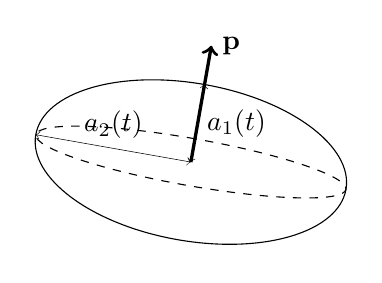
\begin{tikzpicture}[rotate=80]
        \draw(0,0) ellipse (1 cm and 2 cm);
        \draw[dashed](0,0) ellipse (0.3 cm and 2 cm);
        \draw[<->,very thin](0,0) --++ (1,0)node[midway,right]{$a_1(t)$};
        \draw[->,very thick](0,0) --++ (1.5,0)node[right]{$\textbf{p}$};
        \draw[<->,very thin](0,0) --++ (0,2)node[midway,above]{$a_2(t)$};
    \end{tikzpicture}
    \hfill
    \caption{Scheme of an  oblate spheroid oriented along the unit vector \textbf{p} with $a_1(t)$ and $a_2(t)$ the length of the semi axes of the spheroid.}
\end{figure}


\subsubsection*{The droplet internal velocity}

The internal velocity of a solid elastic particle following a homogeneous linear deformation can be described such as $\textbf{w}_2^0 = \bm\Gamma_\alpha \cdot \textbf{r}$ where we have introduced, $\bm\Gamma_\alpha$, the mean velocity gradient inside the particle, which symmetric part : $\textbf{E}_\alpha$, represents the rate of strain, and skew symmetric part : $\bm\Omega_\alpha$, represents the angular velocity. 
Even through the velocity fields $\textbf{w}_2^0 = \bm\Gamma_\alpha \cdot \textbf{r}$  can apply for liquid deforming droplet, an additional flow is present. 
Indeed, from the solution of the stokes equations we can predict the flow within a spherical isolated drop immersed in an unbounded fluid. 
Especially, we know that an solated droplet in translation exhibit internal motion known as Hill vortexes, see \ref{fig:flowlines} (b). 
For a drop immersed in an unbounded linear flow we can also derive an analytical solution such that $\textbf{w}_2^0 \sim \textbf{rrr}$, see \ref{fig:flowlines} (a). 
Therefore, the droplet's internal velocity fields is constituted with a component accounting for the complex internal motions that does not alter the shape of the drop, and another component that account for the linear deformation of the drop.  
\begin{figure*}
    \centering
    \begin{tikzpicture}
        \node (img3) at (0.6\textwidth,0) {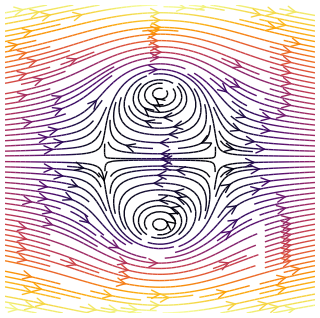
\includegraphics[width=0.3\textwidth,angle=270]{image/Rising_def_Stokes.png}};
        \node (img2) at (0.3\textwidth,0) {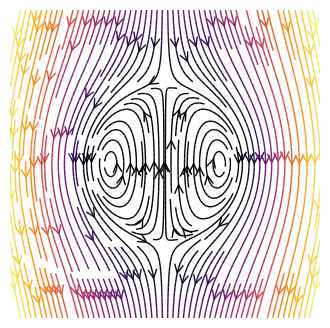
\includegraphics[width=0.3\textwidth]{image/Rising_Stokes.png}};
        % \draw (0.45\textwidth,0)node{$\rightarrow$};
        % \draw (0.45\textwidth,0.4cm)node{$\bm\Gamma_\alpha\cdot \textbf{r}$};
        \node (img1) at (0.0\textwidth,0) {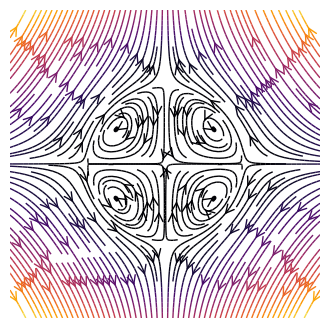
\includegraphics[width=0.3\textwidth]{image/Shear_Stokes.png}};
        \draw (img3.south)node{(c)};
        \draw (img2.south)node{(b)};
        \draw (img1.south)node{(a)};
    \end{tikzpicture}
    \caption{Three examples of steady state flow lines plots of an isolated droplet immersed into a viscous fluid. 
    (a) Rising sphere in uniform stokes flow (analytical solution in \ref{ap:Translating_sphere}). 
    (b) Fixed droplet in extensional flow (analytical solution in \ref{ap:Translating_sphere}).
    (c) Deformed droplet in rising motion (analytical solution of \citet{taylor1964deformation}). }
\end{figure*}
Consequently, the particle internal velocity might be written, 
\begin{equation}
    \textbf{w}_{2,i}^0(\textbf{x}_\alpha)
    = \bm\Gamma_{\alpha,ik}(t) \cdot \textbf{r}_k
    + \textbf{w}^{s}_{2,i}(t,\textbf{r})
    =\bm{\Omega}_{\alpha,ik}\cdot \textbf{r}_k
    + \textbf{E}_{\alpha,ik} \cdot \textbf{r}_k
    + \textbf{w}^{s}_{2,i}(t,\textbf{r})
\end{equation}
Where we introduced the vector $\textbf{w}^{s}_2(t,\textbf{r}) =\textbf{w}^{0}_{2,i}(t,\textbf{r})  - \bm\Gamma_{\alpha,ik}(t) \cdot \textbf{r}_k$ which represents all the internal motions that does not alter the drop's shape. 
Examples of such motions are displayed \ref{fig:flowlines}. 


From now on we consider that the internal velocity $\textbf{w}^{s}_2(t,\textbf{r})$ is not part of the particles unknown, but a function entirely determined by the particle and flow properties such that $\textbf{w}^{s}_2(t,\textbf{r}) =f_\textbf{w}(\textbf{u}_\alpha,\textbf{C}_\alpha,\bm\Gamma_\alpha,\textbf{u}_1,\bm \Gamma_1,\phi_2) $, where $\bm\Gamma_1 = \grad \textbf{u}_1$ and $\textbf{u}_1$ is the mean velocity fields evaluated at the particle position. 
As it is demonstrated in \ref{ap:Translating_sphere} the internal motion of an isolated spherical drop such as the one in \ref{eq:def_vel} might be determined theoretically from the relative motion and flow fields gradient in the limit of low Reynolds number.
We assume that such a relation exist for other regime. 
Consequently, The particle mean velocity gradient $\bm\Gamma_\alpha$ and its conformation tensor $\textbf C_\alpha$ are the only unknown of our problem. 
Therefore, we need to provide two equations, one for $\textbf{C}_\alpha$ and another for $\bm\Gamma_\alpha$. 

\subsubsection*{Kinematic and dynamic of a deformable spheroid}

The evolution of $\textbf{C}_\alpha$ and $\bm\Gamma_\alpha$ will be described by the second moment of mass and first moment of momentum equation.
Consequently, we must reformulate the terms in \ref{eq:dt_M_alpha} and \ref{eq:dt_P_alpha} in terms of $\textbf{C}_\alpha$ and $\bm\Gamma_\alpha$. 
The integrals constitutive of these moments equations can be written, 
\begin{align}
    \intO{(\textbf{rw}_2^0 )_{ij}+ (\textbf{w}_2^0 \textbf{r})_{ij}} 
    = \textbf{C}_{\alpha,ik} \cdot \bm\Gamma_{\alpha,kj}
    +  \bm\Gamma_{\alpha,ki} \cdot \textbf{C}_{\alpha,jk}
    +  \bm\Gamma_{\alpha,ij} + \bm\Gamma_{\alpha,ij}
    \\
    \intO{\rho_2 \textbf{w}_{2,i}^0\textbf{w}_{2,j}^0}
    = \frac{m_\alpha a^2}{5}[
        \bm\Gamma_{\alpha,lj}\bm\Gamma_{\alpha,ki} \textbf{C}_{\alpha,kl} 
        + \bm\Gamma_{\alpha,kj}\bm\Gamma_{\alpha,ki} 
        % + f_\textbf{ww}(\textbf{u}_\alpha,\textbf{C}_\alpha,\bm\Gamma_\alpha,\textbf{u}_1,\bm \Gamma_1,\phi_2)
        + f_\textbf{ww}(\textbf{u}_\alpha,\textbf{C}_\alpha,\bm\Gamma_\alpha,\textbf{u}_1,\bm \Gamma_1,\phi_2)
        ]
    \\
    \intO{\bm\sigma_{2,ij}^0}
    =
    % -\intO{p_2^0} \textbf{I}_{ij}
    \mu_2 v_\alpha [\bm\Gamma_{\alpha,ij} + \bm\Gamma_{\alpha,ij}
    + f_{\bm{\sigma}}(\textbf{u}_\alpha,\textbf{C}_\alpha,\bm\Gamma_\alpha,\textbf{u}_1,\bm \Gamma_1,\phi_2)]
    % + \textbf{I}_{ij}\intO{p_2^0} 
    \\
    \intS{\bm\sigma_{I,ij}^0}
    = \frac{2 \gamma v_\alpha }{a} \textbf{I}_{ij} - \frac{4 \gamma v_\alpha }{5 a} \textbf{C}_{\alpha,ij}
    +\mathcal(|\textbf{C}|^2)\\
    \intS{\textbf{r}\bm\sigma_1^0\cdot \textbf{n}_2}
    = 
    \frac{1}{2}\intS{(\textbf{r}\bm\sigma_1^0-\bm\sigma_1^0\textbf{r})\cdot \textbf{n}_2}
    + \frac{1}{2}\intS{(\textbf{r}\bm\sigma_1^0+\bm\sigma_1^0\textbf{r})\cdot \textbf{n}_2}
    % \textbf{M}(\textbf{u}_\alpha,\textbf{C}_\alpha,\bm\Gamma_\alpha,\textbf{u}_1,\bm \Gamma_1,\phi_2)
\end{align}
\tb{carry the actual decomposition with the velocity components }
\tb{mettre sous forme plus simple et expliquer l'osciallater sous forme 1d}
First, as discussed above only the deforming motion contribute to the symmetric part of the moment of momentum, we could therefore express it explicitly in terms of the particle unknown. 
Regarding the first moment of the surface tension, it has been computed analytically carrying a surface integral on the ellipsoidal surface of the droplet. 
Since, the droplets remain spheroidal under small deformation we choose to approximate $\intS{\bm\sigma_I^0}$ with its first order Taylor series in $\textbf{C}_\alpha$ without lost of generality.
Note that our expression of $\intS{\bm\sigma_I^0}$ is in agreement with \citet{lhuillier1987phenomenology} if one account for the slight difference of his definition of the deformation tensor which is half of $\textbf{C}_{\alpha}$. 
% in which our $\textbf{C}_\alpha$ is twice his, in the limit of small \textbf{C}_\alpha.
For the expression of $\intO{\rho_2 \textbf{w}_{2,i}^0\textbf{w}_{2,j}^0}$, $ \intO{\bm\sigma_{2,ij}^0}$ we had to introduce two unknown functions, $f_\textbf{ww}$, $f_{\bm{\sigma}}$, which vanish when $\textbf{w}^s_2 =0$. 
Therefore, these expressions are a sum of a function involving $\bm\Gamma_\alpha$ and an unknown part which depend on the parameters of the problem and need to be closed. 
The expression of $\intO{\rho_2 \textbf{w}_{2,i}^0\textbf{w}_{2,j}^0}$, $ \intO{\bm\sigma_{2,ij}^0}$ and $\intS{\textbf{r}\bm\sigma_1^0\cdot \textbf{n}_2}$ are very problem dependent. 
To provide a clearer example we computed these terms in \ref{ap:Translating_sphere} in the simplified scenario of an isolated droplet in a general linear flow. 

% The most common example is the expression for first moment \textbf{M}, which has been widely investigated in the pure straining situation, an example is given in \ref{ap:Translating_sphere} for spherical drop, and in \citet{raja2010inertial} for slightly deformable droplet in inertial flows. 
% It is important to notice that these functions are dependent of the relative drop-carrier fluid velocity, in such a way that the momentum and first moment of momentum are linked through the function $f_{\textbf{ww}},f_{\bm{\sigma}}$ and $\intS{\textbf{r}\bm\sigma_1^0\cdot \textbf{n}_2}$. 
% Indeed, even if it has been uniquely studied in pure linear flows, the relative motion of a particle might generate a first moment on its surface. 


At this point it wouldn't be wise trying to find an expression for each of these unknown functions in such a generality. 
Instead, we expose the unclosed set of equation of motions for spheroidal particles. 
In addition to the previously exposed equations (mass, momentum and energy equation) this system is constituted of three equations, one for $\textbf{C}_\alpha$ and two equation for the moment of momentum, the symmetric and skew-symmetric moment of momentum. 
% These read, 
\begin{align*}
    \ddt \textbf{C}_{\alpha,ij}
    = \textbf{C}_{\alpha,ik} \cdot \bm\Gamma_{\alpha,kj}
    +  \bm\Gamma_{\alpha,ki} \cdot \textbf{C}_{\alpha,jk},\\
    \frac{a^2  m_\alpha}{5} \ddt( \textbf{C}_{ik} \cdot \bm\Gamma_{\alpha,kj}
    -  \bm\Gamma_{\alpha,ki} \cdot \textbf{C}_{jk})
    =  \intS{(\textbf{r}\bm\sigma_2^0- \bm\sigma_2^0\textbf{r})\cdot \textbf{n}}\\
    \frac{m_\alpha a^2}{5}\ddt^2 \textbf{C}_\alpha
    - \frac{m_\alpha a^2}{5}[
    \bm\Gamma_{\alpha,lj}\bm\Gamma_{\alpha,ki} \textbf{C}_{\alpha,kl} + f_\textbf{ww}]
    + \mu_2 v_\alpha [(\bm \Gamma_{p,ij}+\bm \Gamma_{p,ji})
    + f_{\bm{\sigma}}]\\
    + \frac{2 \gamma v_\alpha }{a} \textbf{I}_{ij} 
    - \frac{4 \gamma v_\alpha }{5 a} (\textbf{C}_{ij} - \textbf{I}_{ij})
    = \intS{(\textbf{r}\bm\sigma_2^0+ \bm\sigma_2^0\textbf{r})\cdot \textbf{n}}
    % + \textbf{I}_{ij}\intO{p_2^0}
\end{align*}
% Where we placed the unknown function at the right hands side of these equations. 
Now, we would like to propose a more intuitive interpretation of the mass and momentum equations.
To that end, we make the problem dimensionless by introducing, 
the \textit{Capillary number} $Ca= \frac{\mu_1 U}{\gamma}$, The viscosity ratio $\lambda = \mu_2/\mu_1$, the density ratio $\zeta = \rho_2/\rho_1$ and the Reynolds number $Re = \frac{a U \rho_1}{\mu_1}$, with $U$ as the velocity scale. 
%  such that  $\bm\Gamma_\alpha'  = \frac{a}{U}\bm\Gamma$, and $\tau_a$ the timescale related to the drop shape evolution.
In the low Reynolds regime the first moment of surface traction forces will be proportional to a viscous stress (see \ref{ap:Translating_sphere}), therefore :$\intS{\textbf{r}\bm\sigma_2^0\cdot \textbf{n}} =\mu_1  \tau v_\alpha \intS{\textbf{r}\bm\sigma_2^0\cdot \textbf{n}}^*$, with $\tau$ the inverse timescale of the external solicitation.
The ratio between the external flow scale $\tau$ and the drop timescale $\tau_a$ is noted $\beta$. 
With that in mind, \ref{eq:dt_M_alpha}, \ref{eq:dt_mu_alpha} and \ref{eq:dt_S_alpha} might be written :
\begin{align}
    \beta \ddt \textbf{C}_{\alpha,ij}
    - \textbf{C}_{\alpha,ik} \cdot \bm\Gamma_{\alpha,kj}^*
    - \bm\Gamma_{\alpha,ki}^* \cdot \textbf{C}_{\alpha,jk},
    = 
    \bm\Gamma_{\alpha,ij}^*
    +  \bm\Gamma_{\alpha,ji}^*\\
    Re \zeta \beta \ddt( \textbf{C}_{\alpha,ik} \cdot \bm\Gamma_{\alpha,kj}^*
    -  \bm\Gamma_{\alpha,ki}^* \cdot \textbf{C}_{\alpha,jk}
    + \bm\Gamma_{\alpha,ji} - \bm\Gamma_{\alpha,ij})
    =  \intS{(\textbf{r}\bm\sigma_2^0- \bm\sigma_2^0\textbf{r})\cdot \textbf{n}}^*\\
    \zeta Re \frac{1}{5}  
    \left[
        \frac{1}{2}\beta^2 \ddt^2_* \textbf{C}_\alpha
        - \bm\Gamma_{\alpha,lj}^* \bm\Gamma_{\alpha,ki}^* \textbf{C}_{\alpha,kl}^* 
        - \bm\Gamma_{\alpha,kj}^* \bm\Gamma_{\alpha,ki}^* 
        - f_\textbf{ww}
    \right]\nonumber\\
    + \lambda \left[
        \beta \ddt \textbf{C}_{\alpha,ij}
        -\textbf{C}_{\alpha,ik} \cdot \bm\Gamma_{\alpha,kj}
        - \bm\Gamma_{\alpha,ki}^* \cdot \textbf{C}_{\alpha,jk},
        + f_{\bm{\sigma}}
    \right]\nonumber\\
    - \frac{1}{Ca}\left[
        \frac{4}{5} \textbf{C}_{\alpha,ij}
        +2 \textbf{I}_{ij} 
    \right]
    =
    \frac{1}{2}\intS{(\textbf{r}\bm\sigma_1^0+ \bm\sigma_1^0\textbf{r})\cdot \textbf{n}}^*
\end{align}
\tb{at this point it is not usefull to introduce the substitution in the last equaiton instead explain that it is proportional to the derivative in the limit}
The second moment of mass \ref{eq:dt_Cs}, is consistent with the equation found by \citet{goddard1967nonlinear} and \citet{lhuillier1987phenomenology}. 
Following, \citet{goddard1967nonlinear}  terminology, the left-hand side of \ref{eq:dt_Cs} is referred as the \textit{convected} derivative of $\textbf{C}^*_\alpha$. 
Therefore, the \textit{convected} derivative of $\textbf{C}_\alpha$ is equal to the rate of strain of the particle. 
The skew-symmetric part of the first moment of momentum \ref{eq:dt2_C}, it is basically the angular momentum balance of a non-spherical object. 
The right-hands side accounting for the external torque contribution. 
The symmetric part however has the form of a non-linear forced harmonic oscillatory equation for the droplet deformation. 
Indeed, the first groups of terms on the left-hand side represent the inertial contribution of the droplet internal fluid. 
It is made of a second order derivative plus non-linear terms in $\bm\Gamma_\alpha$. 
The second groups of terms is internal viscous contribution that arise directly from the definition of the stress \ref{eq:sigma_2_def}. 
It vanishes for small viscosity ration and is linear in the first derivative of $\textbf{C}_\alpha$. 
The last term on the left-hand side is the elastic response from the interface which is negligible for high capillary number $Ca \to \infty$. 
Then on right-hand side of the equation we find the first moment of surface force, $\intS{(\textbf{r}\bm\sigma_1^0+ \bm\sigma_1^0\textbf{r})\cdot \textbf{n}}^*$ which has an unknown expression at this stage. 
\ref{eq:dt2_C} might be regarded as a second order harmonic equation with non-linear contributions. 
However, the unknown function $f_\textbf{ww},\ f_{\bm{\sigma}}$ and $\intS{(\textbf{r}\bm\sigma_1^0+ \bm\sigma_1^0\textbf{r})\cdot \textbf{n}}^*$ are in general function of $\textbf{C}_\alpha$ and its higher derivatives of $\textbf{C}_\alpha$.   
Therefore, at this stage it is impossible to predict the nature of the harmonic regime followed by the droplet. 
To conclude on this matter one must find an expression for all this closure as well as determinate the impact of the non-linear terms.

We now examine the specific case studied by \citet{lamb1924hydrodynamics} where he considered no external contribution around the particle, therefore, $\intS{(\textbf{r}\bm\sigma_1^0+ \bm\sigma_1^0\textbf{r})\cdot \textbf{n}}^* = 0$.
It is found, that the amplitude of the second order harmonic mode of deformation, noted $\epsilon_2$, follows the second order partial differential equations,  
\begin{equation*}
    \ddt^2{\epsilon_2}
    + 2\lambda_2 \ddt \epsilon_2
    + \omega_2^2 \epsilon_2
     = 0,
\end{equation*}
where $\lambda_2$ and $\omega_2$ are the damping and frequency of coefficient defined as, 
\begin{align*}
    \lambda_2 = 5 \frac{\mu_2}{\rho_2a^2},
    && \omega_2 = \sqrt{8 \frac{\mu_2}{\rho_2 a^2}}.
\end{align*}
Where this equation has been obtained in the linear deformation regime for $\epsilon_2 \ll 1$. 
When multiplying \ref{eq:dt2_C} by, $\frac{10}{\zeta Re}$ we indeed find the exact same coefficient $\lambda_2$ and $\omega_2^2$ in front of, $\ddt \textbf{C}_{\alpha,ij}$ and $\textbf{C}_{\alpha,ij}$, respectively. 
In the limit of small $\textbf{C}_\alpha$, only these linear terms remain, therefore consistent with the reference work of \citet{lamb1924hydrodynamics}. 
\ref{eq:dt2_C} is somewhat more general than lamb's solution since it is expressed in an arbitrary reference frame. 
Which will prove to be useful in \ref{sec:Exemples} were we apply ensemble average on these quantities. 
However, with this equation we are able to describe only the second oscillatory mode. 
To study higher order modes one must use higher moment of momentum equations. 

In the past studies, the coupling between translational and oscillating nature of rising bubbles or droplets have been investigated \citet{lalanne2013effect}. 
For an isolated spherical droplet in translation through a stokes or potential flow we know that $
    f_\textbf{ww}
    = \frac{m_\alpha}{140 (\lambda +1)^2}
    (7 \textbf{u}_{\alpha 1} \textbf{u}_{\alpha 1} + \textbf{u}_{\alpha 1}\cdot \textbf{u}_{\alpha 1}\textbf{I})$, 
(see \ref{ap:Translating_sphere}). 
It is reasonable to guess that for a slightly spheroidal droplet in translation the expression might preserve the same form. 
Indeed, a coefficient related to $\textbf{C}_\alpha$ might appear in the expression nevertheless the overall contribution must be still proportional to $\textbf{u}_{\alpha 1} \textbf{u}_{\alpha 1}$. 
Likewise, for an inertial drops, it might be found that 
$\intS{(\textbf{r}\bm\sigma_1^0+ \bm\sigma_1^0\textbf{r})\cdot \textbf{n}}^* \sim A \textbf{u}_{\alpha 1} \textbf{u}_{\alpha 1} + B \textbf{u}_{\alpha 1} \cdot \textbf{u}_{\alpha 1}$ where $A$ and $B$ are constant. 
Indeed, the translational motion a spherical particle at slight inertia induce an overall unbalance stress on the surface of the particle generating a first moment \citet{taylor1964deformation}. 
The point is that the yet unknown closures, will help us bridge translational and drop's straining motions. 
Therefore, injecting these expressions into \ref{eq:dt2_C} would be a first step to accomplish a coupling between oscillating, or deforming motion with translating motion.
This is the subject of the last section. 
Obviously, now that we obtained a general formulation for the dynamic of the droplets' deformation, the most challenging aspect is to find expressions for closure terms. 


\subsubsection*{The particle internal energy balance.}

The surface of the particles, and internal kinetic energy can be written in this context as, 
\begin{align*}
    \beta \ddt \textbf{C}_{\alpha,ij}
    - \textbf{C}_{\alpha,ik} \cdot \bm\Gamma_{\alpha,kj}^*
    - \bm\Gamma_{\alpha,ki}^* \cdot \textbf{C}_{\alpha,jk},
    = 
    2\textbf{E}_{\alpha,ij}\\
    \intO{\rho_2 \textbf{w}_{2,i}^0\textbf{w}_{2,i}^0}
    = \frac{m_\alpha a^2}{5}[
        \bm\Gamma_{\alpha,li}\bm\Gamma_{\alpha,ki} \textbf{C}_{\alpha,kl} 
        + \bm\Gamma_{\alpha,ki}\bm\Gamma_{\alpha,ki} 
        + f_\textbf{ww}(\textbf{u}_\alpha,\textbf{C}_\alpha,\bm\Gamma_\alpha,\textbf{u}_1,\bm \Gamma_1,\phi_2)
        ]
    \\
    \intO{\bm\sigma_{2,ij}^0:\grad \textbf{u}_2^0}
    = 2 \mu_2 \intO{\textbf{e}_2^0:\textbf{e}_2^0}
    = 2\mu_2v_\alpha\left[ \textbf{E}_{\alpha,ij}\textbf{E}_{\alpha,ij}
    + f_{\textbf{e}}\right]\\
    % -\intO{p_2^0} \textbf{I}_{ij}
    \mu_2 v_\alpha [\textbf{E}_{\alpha,ij}
    + f_{\bm{\sigma}}(\textbf{u}_\alpha,\textbf{C}_\alpha,\bm\Gamma_\alpha,\textbf{u}_1,\bm \Gamma_1,\phi_2)]
    % + \textbf{I}_{ij}\intO{p_2^0} 
    \\
    s_\alpha \gamma
    = 
    \frac{3 \gamma v_\alpha }{a}\left[
        1
        + \frac{1}{20}\textbf{C}_\alpha:\textbf{C}_\alpha
    \right]
\end{align*}

\begin{equation}
    \ddt (W_\alpha + \gamma s_\alpha)
    + \intO{ \bm{\sigma}_2^0 : \grad\textbf{u}_2^0 }
    =\intS{\textbf{w}_1^0 \cdot \bm{\sigma}_1^0 \cdot \textbf{n}_2} 
\end{equation}

In conclusion, we have demonstrated how the first and second moment of momentum and mass equation can be used to describe the second mode oscillatory motion of a spheroidal drop in a Galilean reference frame. 
Therefore, the moment of momentum is a quantity of utmost importance for all kinds of particles with variable shape or volume.
This isn't limited to the momentum distribution, but all kind of properties can be described that way. 
In fact, if one wish to describe the first moment of the distribution of any local quantity $f_2^0$ and $f_I^0$ over the surface or volume of the particle, he must use the first moments' conservation equations. 
As an example, the mean concentration and distribution of surfactants on the bubbles' surface have a significant impact on the mass transfer rate between the dispersed and continuous phases.
In this case first moment of surfactant concentration could be considered here to track the evolution of the surfactant concentration and orientation over the particle surface, which would enable us to compute a better approximation of the drag force coefficient. 

% 
% \section{Re-derivation but more easy}
% \label{ap:local_basis_eq}

% All these went way to complicated. 
% So here is a more consize derivation that does keep track of the physics. 
% We describe the geometry of the particle with the second moment of mass tensor, 
% \begin{equation*}
%     M_{\alpha,ij} 
%     =\frac{m_\alpha a^2}{5} M_{\alpha,ij}^*
%     = \frac{m_\alpha a^2}{5}\left[
%         \left(
%             \frac{a_1}{a}
%         \right)^2 p_i p_j
%         + 
%         \left(
%             \frac{a_1}{a}
%         \right)^2(\delta_{ij}-  p_i p_j)
%     \right]
% \end{equation*}
% This tensor has several notable properties, the volume conservation : $a_1 a_2^2 = a^3$ which means that $\textbf{M}_\alpha^*$ has two eigenvalues linked through $M^1 = (M^2)^{-2}$ or $M^2 = (M^1)^(-1/2)$. 
% At small deformation, i.e. $M_1 - 1\ll 1$ we therefore have $M^1 = 1 - (M^1-1)/2$.
% This ultimately means that at small deformation the trace is a constant namely $M_{ij} \delta_{ij} = 3+\mathcal{O}((M^1 -1)^2)$. 




% Let's now reformulate the integral of the problem namely, 
% \begin{align}
%     \intO{(\textbf{rw}_ 2^0 )_{ij}+ (\textbf{w}_2^0 \textbf{r})_{ij}} 
%     = \textbf{M}_{\alpha,ik} \cdot \bm\Gamma_{\alpha,jk}
%         +  \bm\Gamma_{\alpha,ik} \cdot \textbf{M}_{\alpha,jk}
%     \\
%     \intO{\rho_2 \textbf{w}_{2,i}^0\textbf{w}_{2,j}^0}
%     = \bm\Gamma_{\alpha,jl}\bm\Gamma_{\alpha,ik} \textbf{M}_{\alpha,kl}  
%         +\intO{\rho_2 \textbf{w}_{2,i}^s\textbf{w}_{2,j}^s}
%     \\
%     \intO{\bm\sigma_{2,ij}^0}
%     =
%     2 \mu_2 v_\alpha \textbf{E}_{\alpha,ij}
%     - \intO{p_2^0} \textbf{I}_{ij}
%     + \mu_2 \intS{(\textbf{n}_i \textbf{w}_{2,j}^s + \textbf{n}_j \textbf{w}_{2,i}^s)}
%     \\
%     \intS{\bm\sigma_{I,ij}^0}
%     = \frac{\gamma v_\alpha }{a} \left[
%         2\textbf{I}_{ij} 
%         - \frac{4  }{5} (\textbf{M}_{\alpha,ij}^* - \textbf{I}_{\alpha,ij})
%     \right]
%     +\mathcal(O)(\textbf{C}\cdot \textbf{C})\\
%     s_\alpha 
%     = 4\pi a^2 (1+\frac{\textbf{C}:\textbf{C}}{15})
% \end{align}
% for the surface tension term is made of two terms, one corresponding to Laplace pressure and the other to the deviatoric stress. 




% The equation for the orientation, second moment of mass torque, symmetric moment of momentum and trace of the moment of momentum reads, 
% \begin{align*}
%     \ddt \textbf{pp}_{\alpha,ij}
%     = \textbf{pp}_{\alpha,ik} \cdot \bm\Omega_{\alpha,jk}
%     +  \bm\Omega_{\alpha,ik} \cdot \textbf{pp}_{\alpha,jk}\\
%     \ddt \textbf{M}_{\alpha,ij}
%     = \textbf{M}_{\alpha,ik} \cdot \bm\Gamma_{\alpha,jk}
%     +  \bm\Gamma_{\alpha,ik} \cdot \textbf{M}_{\alpha,jk}\\
%     \ddt (\textbf{I}_{\alpha,ik}\bm\omega_{\alpha,k} )
%     = 
%     \intS{(\textbf{r}\times\bm\sigma_1^0\cdot \textbf{n})_i} \\
%     \frac{1}{2}\ddt^2 \textbf{M}_{\alpha,ij}
%     -  \bm\Gamma_{\alpha,jl}\bm\Gamma_{\alpha,ik} \textbf{M}_{\alpha,kl}  
%     + 2 \mu_2 v_\alpha \textbf{E}_{\alpha,ij}
%     + \frac{\gamma v_\alpha }{a} \left[
%     2\textbf{I}_{ij} 
%     - \frac{4 \gamma v_\alpha }{5 a} (\textbf{M}_{\alpha,ij}^* - \textbf{I}_{\alpha,ij})
%     \right]\\
%     = 
%     \frac{1}{2}\intS{(\textbf{r}\bm\sigma_1^0 + \bm\sigma_1^0\textbf{r})\cdot \textbf{n}} 
%     + \intO{\rho_2 \textbf{w}_{2,i}^s\textbf{w}_{2,j}^s}
%     + \intO{p_2^0} \textbf{I}_{ij}
%     - \mu_2 \intS{(\textbf{n}_i \textbf{w}_{2,j}^s + \textbf{n}_j \textbf{w}_{2,i}^s)}\\
%     % \frac{1}{2}\ddt^2 \textbf{M}_{\alpha,mm}
%     -  \bm\Gamma_{\alpha,ml}\bm\Gamma_{\alpha,mk} \textbf{M}_{\alpha,kl}  
%     + \frac{\gamma v_\alpha }{a} 
%     % \left[
%     2\textbf{I}_{mm} 
%     % - \frac{4 }{5 } (\textbf{M}_{\alpha,mm}^* - \textbf{I}_{\alpha,mm})
%     % \right]
%     % \\
%     = 
%     \intS{\textbf{r}_m\cdot\bm\sigma_{1,mk}^0\cdot \textbf{n}_k} 
%     + \intO{\rho_2 \textbf{w}_{2,m}^s\cdot \textbf{w}_{2,m}^s}
%     + \intO{p_2^0} \textbf{I}_{mm}
% \end{align*}

% As the derivative of $M_{ij}$ in these equations actually takes in account the change of orientation of the particle it might be useful to re-derive these equations in the eigenbasis of the matrix $M_{ij}$

% To the first order in deformation the deviatoric part reads, 
% \begin{align*}
%     \frac{1}{2}\ddt^2 \textbf{M}_{\alpha,ij}
%     -   \textbf{M}_{\alpha,kl} 
%     (\bm\Gamma_{\alpha,jl}\bm\Gamma_{\alpha,ik}  
%     - \frac{1}{3}
%     \bm\Gamma_{\alpha,ml}\bm\Gamma_{\alpha,mk}  
%     \textbf{I}_{ij}
%     )
%     + 2 \mu_2 v_\alpha \textbf{E}_{\alpha,ij}
%     - \frac{\gamma v_\alpha }{a} 
%     \frac{4  }{5} (\textbf{M}_{\alpha,ij}- \textbf{I}_{ij})
%     \\
%     = 
%     \frac{1}{2}\intS{(\textbf{r}\bm\sigma_1^0 + \bm\sigma_1^0\textbf{r} - \frac{2}{3}\textbf{r}\cdot \bm\sigma_1^0 \textbf{I})\cdot \textbf{n}} 
%     + \intO{\rho_2 (\textbf{w}_{2,i}^s\textbf{w}_{2,j}^s - \frac{1}{3}\textbf{w}_{2,m}^s\textbf{w}_{2,m}^s \textbf{I}_{ij}) }
%     - \mu_2 \intS{(\textbf{n}_i \textbf{w}_{2,j}^s + \textbf{n}_j \textbf{w}_{2,i}^s)}\\
% \end{align*}
% It can be somewhat useful to extract the proportionality coefficient of each terms. 
% Denotining dimensionless qte by a $*$ we have, 
% \begin{align*}
%     \frac{\rho_2 a^2}{5 \tau^2}\left[\frac{1}{2}\ddt^2 \textbf{M}_{\alpha,ij}^*
%     -  \bm\Gamma_{\alpha,jl}^*\bm\Gamma_{\alpha,ik}^* \textbf{M}_{\alpha,kl}^*
%     \right]  
%     + \frac{2 \mu_2  }{\tau} \textbf{E}_{\alpha,ij}^*
%     + \frac{\gamma  }{a} \left[
%     2\textbf{I}_{ij} 
%     - \frac{4 }{5} (\textbf{M}_{\alpha,ij}^* - \textbf{I}_{\alpha,ij})
%     \right]\\
%     = 
%     \frac{1}{2}\intS{(\textbf{r}\bm\sigma_1^0 + \bm\sigma_1^0\textbf{r})\cdot \textbf{n}} 
%     + \intO{\rho_2 \textbf{w}_{2,i}^s\textbf{w}_{2,j}^s}
%     + \intO{p_2^0} \textbf{I}_{ij}
%     - \mu_2 \intS{(\textbf{n}_i \textbf{w}_{2,j}^s + \textbf{n}_j \textbf{w}_{2,i}^s)}\\
% \end{align*}

% The forcing terms are really problem dependent. 
% Thus, at this stage it cannot be scaled in terms of timescale. 

% In order to be more consis, we may write :
% \begin{align*}
%     \textbf{F}_{ij}(\textbf{w}^s,\bm\sigma_1^0)
%     = 
%     \frac{1}{2}\intS{(\textbf{r}\bm\sigma_1^0 + \bm\sigma_1^0\textbf{r} - \frac{2}{3}\textbf{r}\cdot \bm\sigma_1^0 \textbf{I})\cdot \textbf{n}} 
%     + \intO{\rho_2 (\textbf{w}_{2,i}^s\textbf{w}_{2,j}^s - \frac{1}{3}\textbf{w}_{2,m}^s\textbf{w}_{2,m}^s \textbf{I}_{ij}) }
%     - \mu_2 \intS{(\textbf{n}_i \textbf{w}_{2,j}^s + \textbf{n}_j \textbf{w}_{2,i}^s)}\\
% \end{align*} 
% Indicating that the forcing term is related to the exterior contribution and the external stresses. 

% \begin{align*}
%     \ddt^2 \textbf{M}_{\alpha,ij}^*
%     -2  \textbf{M}_{\alpha,kl}^* 
%     (\bm\Gamma_{\alpha,jl}^*\bm\Gamma_{\alpha,ik}^*  
%     - \frac{1}{3}
%     \bm\Gamma_{\alpha,ml}^*\bm\Gamma_{\alpha,mk}^*  
%     \textbf{I}_{ij}
%     )
%     + \frac{10 \mu_2 \tau}{ \rho_2 a^2} 2\textbf{E}_{\alpha,ij}^*
%     - 8 \frac{\tau^2 \gamma  }{\rho_2 a^3} 
%      (\textbf{M}_{\alpha,ij}^*- \textbf{I}_{ij})\\
%     = 
%     \frac{\tau^2 10}{a^2 m_\alpha}
%     \left[\textbf{F}_{\sigma_1, ij}
%     + \textbf{F}_{ww, ij}
%     + \textbf{F}_{\sigma_2, ij}\right]
% \end{align*}

% All these unclose term are really problem dependent, for now all we now is that at low Reynolds number we are in the viscous regime, besides this external flow that drives these scales. 
% Meaning that, 
% \begin{align*}
%     \intO{\rho_2 \textbf{w}_{2,i}^0\textbf{w}_{2,j}^0}
%     \sim \frac{m_\alpha a^2}{\tau_u^2} \textbf{F}_{ww}^*
%     \\
%     \mu_2 \intS{(\textbf{n}_i \textbf{w}_{2,j}^s + \textbf{n}_j \textbf{w}_{2,i}^s)}
%     \sim \frac{v_\alpha \mu_2}{\tau_u} \textbf{F}_{e}^*
%     \\
%     \intS{\bm\sigma_1^0 \textbf{rn}}
%     \sim 
%     \frac{v_\alpha \mu_1}{\tau_u} \textbf{F}_{\sigma}^*
% \end{align*} 

% \begin{align*}
%     \ddt^2 \textbf{M}_{\alpha,ij}^*
%     -2  \textbf{M}_{\alpha,kl}^* 
%     (\bm\Gamma_{\alpha,jl}^*\bm\Gamma_{\alpha,ik}^*  
%     - \frac{1}{3}
%     \bm\Gamma_{\alpha,ml}^*\bm\Gamma_{\alpha,mk}^*  
%     \textbf{I}_{ij}
%     )
%     + \frac{10 \mu_2 \tau}{ \rho_2 a^2} 2\textbf{E}_{\alpha,ij}^*
%     - 8 \frac{\tau^2 \gamma  }{\rho_2 a^3} 
%      (\textbf{M}_{\alpha,ij}^*- \textbf{I}_{ij})\\
%     = 
%     \frac{\tau^2 10 \mu_1 }{a^2 \rho_2 \tau_u}
%     \textbf{F}_{\sigma_1, ij}
%     + \frac{\tau^2 10}{\tau_u^2} \textbf{F}_{ww, ij}
%     + \frac{\tau^2 10 \mu_1 }{a^2 \rho_2 \tau_u} \textbf{F}_{\sigma_2, ij}
% \end{align*}


% \subsubsection*{Re-derivation but with dimensionless scaling}

% \begin{align}
%     \intO{(\textbf{rw}_ 2^0 )_{ij}+ (\textbf{w}_2^0 \textbf{r})_{ij}} 
%     = \textbf{M}_{\alpha,ik} \cdot \bm\Gamma_{\alpha,jk}
%         +  \bm\Gamma_{\alpha,ik} \cdot \textbf{M}_{\alpha,jk}
%     \\
%     \intO{\rho_2 \textbf{w}_{2,i}^0\textbf{w}_{2,j}^0}
%     = \bm\Gamma_{\alpha,jl}\bm\Gamma_{\alpha,ik} \textbf{M}_{\alpha,kl}  
%         +\intO{\rho_2 \textbf{w}_{2,i}^s\textbf{w}_{2,j}^s}
%     \\
%     \intO{\bm\sigma_{2,ij}^0}
%     =
%     2 \mu_2 v_\alpha \textbf{E}_{\alpha,ij}
%     - \intO{p_2^0} \textbf{I}_{ij}
%     + \mu_2 \intS{(\textbf{n}_i \textbf{w}_{2,j}^s + \textbf{n}_j \textbf{w}_{2,i}^s)}
%     \\
%     \intS{\bm\sigma_{I,ij}^0}
%     = \frac{\gamma v_\alpha }{a} \left[
%         2\textbf{I}_{ij} 
%         - \frac{4  }{5} (\textbf{M}_{\alpha,ij}^* - \textbf{I}_{\alpha,ij})
%     \right]
%     +\mathcal(O)(\textbf{C}\cdot \textbf{C})\\
%     s_\alpha 
%     = 4\pi a^2 (1+\frac{\textbf{C}:\textbf{C}}{15})
% \end{align}

% Then, 
% \begin{align*}
%     \frac{\rho_2 a^2}{5}\left[
%         \frac{1}{\tau^2}\frac{1}{2}\ddt^2 \textbf{M}_{\alpha,ij}
%     -   \frac{1}{\tau^2}\bm\Gamma_{\alpha,jl}\bm\Gamma_{\alpha,ik} \textbf{M}_{\alpha,kl}  
%     - \frac{1}{\tau_u^2} \textbf{F}_{ww}^*
%     \right]\\
%     + \mu_2  \left[
%         \frac{1}{\tau} 2\textbf{E}_{\alpha,ij}
%     + \frac{1}{\tau_u} \textbf{F}_\sigma^*
%     \right]\\
%     + \frac{\gamma  }{a} \left[
%     2\textbf{I}_{ij} 
%     - \frac{4  }{5} (\textbf{M}_{\alpha,ij}^* - \textbf{I}_{\alpha,ij})
%     \right]\\
%     = 
%     \frac{1}{2}
%     \frac{ \mu_1}{\tau_u} 
%     \textbf{F}_{\sigma_1}^*
%     % \intS{(\textbf{r}\bm\sigma_1^0 + \bm\sigma_1^0\textbf{r})\cdot \textbf{n}} 
%     % + \intO{p_2^0} \textbf{I}_{ij}
% \end{align*}

% which then, 
% \begin{align*}
%     \frac{\rho_2}{\rho_1}\frac{\rho_1 a^2}{5\mu_1\tau_u}\left[
%         \frac{\tau_u^2}{\tau^2}\frac{1}{2}\ddt^2 \textbf{M}_{\alpha,ij}
%     -   \frac{\tau_u^2}{\tau^2}\bm\Gamma_{\alpha,jl}\bm\Gamma_{\alpha,ik} \textbf{M}_{\alpha,kl}  
%     - \textbf{F}_{ww}^*
%     \right]\\
%     + \frac{\mu_2}{\mu_1}  \left[
%         \frac{\tau_u}{\tau} 2\textbf{E}_{\alpha,ij}
%     +  \textbf{F}_\sigma^*
%     \right]\\
%     + \frac{\gamma \tau_u }{a\mu_1} \left[
%     2\textbf{I}_{ij} 
%     - \frac{4  }{5} (\textbf{M}_{\alpha,ij}^* - \textbf{I}_{\alpha,ij})
%     \right]\\
%     = 
%     \frac{1}{2}
%     \textbf{F}_{\sigma_1}^*
%     % \intS{(\textbf{r}\bm\sigma_1^0 + \bm\sigma_1^0\textbf{r})\cdot \textbf{n}} 
%     % + \intO{p_2^0} \textbf{I}_{ij}
% \end{align*}

% In terms of dimensionless groups
% \begin{align*}
%     \zeta Re\left[
%         \beta^2 \frac{1}{2}\ddt^2 \textbf{M}_{\alpha,ij}
%     -   \beta^2 \bm\Gamma_{\alpha,jl}\bm\Gamma_{\alpha,ik} \textbf{M}_{\alpha,kl}  
%     - \textbf{F}_{ww}^*
%     \right]\\
%     + \lambda  \left[
%         \beta 2\textbf{E}_{\alpha,ij}
%     +  \textbf{F}_\sigma^*
%     \right]\\
%     + \frac{1}{Ca} \left[
%     2\textbf{I}_{ij} 
%     - \frac{4  }{5} (\textbf{M}_{\alpha,ij}^* - \textbf{I}_{\alpha,ij})
%     \right]\\
%     = 
%     \frac{1}{2}
%     \textbf{F}_{\sigma_1}^*
%     % \intS{(\textbf{r}\bm\sigma_1^0 + \bm\sigma_1^0\textbf{r})\cdot \textbf{n}} 
%     % + \intO{p_2^0} \textbf{I}_{ij}
% \end{align*}


% \subsubsection*{Slow flows wheer beta equal 0 }

% \textbf{Steady state equillibrium }
% \begin{align*}
%     - \zeta Re \textbf{F}_{ww}^*
%     + \lambda  \textbf{F}_\sigma^*
%     + \frac{1}{Ca} \left[
%     2\textbf{I}_{ij} 
%     - \frac{4  }{5} (\textbf{M}_{\alpha,ij}^* - \textbf{I}_{\alpha,ij})
%     \right]
%     = 
%     \frac{1}{2}
%     \textbf{F}_{\sigma_1}^*
%     % \intS{(\textbf{r}\bm\sigma_1^0 + \bm\sigma_1^0\textbf{r})\cdot \textbf{n}} 
%     % + \intO{p_2^0} \textbf{I}_{ij}
% \end{align*}

% In the last part i want to be able to neglect all the components on the left

% if the reynolds number is indeed negligible we have 

% \begin{align*}
%     + \lambda  \textbf{F}_\sigma^*
%     + \frac{1}{Ca} \left[
%     2\textbf{I}_{ij} 
%     - \frac{4  }{5} (\textbf{M}_{\alpha,ij}^* - \textbf{I}_{\alpha,ij})
%     \right]
%     = 
%     \frac{1}{2}
%     \textbf{F}_{\sigma_1}^*
%     % \intS{(\textbf{r}\bm\sigma_1^0 + \bm\sigma_1^0\textbf{r})\cdot \textbf{n}} 
%     % + \intO{p_2^0} \textbf{I}_{ij}
% \end{align*}
% which give the equillibrium of surface tension internal / external stresses
% This must be respected for almost all steady state equilibrium presented in appendix
% It is clear that if either $\lambda = 0$ or that we are looking for the fluid phase stress then the int on the left vanish. 
% And we are left with an equillibrium between surface tension and stresslet

% \tb{In this regime one might recognize Laplace law}

% \textbf{Drop in air }
% \begin{align*}
%     \zeta Re\left[
%          \frac{1}{2}\ddt^2 \textbf{M}_{\alpha,ij}
%     -    \bm\Gamma_{\alpha,jl}\bm\Gamma_{\alpha,ik} \textbf{M}_{\alpha,kl}  
%     \right]
%     +   
%         \frac{\lambda}{\beta} 2\textbf{E}_{\alpha,ij}
%     + \frac{1}{Ca\beta^2} \left[
%     2\textbf{I}_{ij} 
%     - \frac{4  }{5} (\textbf{M}_{\alpha,ij}^* - \textbf{I}_{\alpha,ij})
%     \right]\\
%     = 
%     0 
% \end{align*}
% Indeed, in this case we still consier that the surface tension is comparable with the ratio of time scale of course. 
% Besides, 
% \tb{In this regime one might recognize Lamb's equation }



\section{The local basis equation}
\label{ap:local_basis_eq}

In this appendix we give details about the derivation of the angular momentum and rate of strain equations in the local basis of the particle. 

Firstly, we consider that any second order tensor $\textbf{A}$ can be expressed in the basis formed by the unit vectors $\{\textbf{p}^0,\textbf{p}^1,\textbf{p}^2\}$, which form an orthonormal basis. 
The first vector $\textbf{p}^0$ corresponds to the vector of the particle orientation. 
The vector $\textbf{p}^1$ and $\textbf{p}^2$ are defined such that $\textbf{p}^1 \times \textbf{p} =\textbf{p}^1 \times \textbf{p}^2=\textbf{p}^2 \times \textbf{p} =0$. 
Since, the vectors $\{\textbf{p}^0,\textbf{p}^1,\textbf{p}^2\}$ form a linearly independent family, any arbitrary second order tensor  \textbf{A} can be written, 
\begin{equation}
    A_{ij}
    = 
    A^{ab}
    p_i^a
    p_j^b.
\end{equation}
The indices in superscript are used to denote the local basis tensors  components and operations, such that $A^{ab}$ corresponds to the components of \textbf{A} in the basis $\{\textbf{p}^0,\textbf{p}^1,\textbf{p}^2\}$. 
Additionally, we also used the Einstein summation convention for the indices in superscript. 
Note that the components $A^{ab}$ can be obtained from \textbf{A} applying the double contracted product,  
\begin{equation*}
    A_{ij} 
    p_i^a
    p_j^b
    = 
    A^{cd}
    p_i^c
    p_j^d
    p_i^a
    p_j^b
    = 
    A^{ab}
\end{equation*}
From there it is easy to understand that to obtain the evolution equation in the eigenbasis one has to multiply the previous set of equation with $p_i^ap_j^b$. 

Let us recall some tensor properties. 
Note that if $\bm{\Omega}$ is defined as a skew-symmetric tensor, such that, 
\begin{equation}
    \Omega_{ij} = \frac{1}{2} [A_{ij}-A_ji],
\end{equation}
then, the tensor $\bm\Omega$ written in the local basis will also be skew-symmetric, thus we have
\begin{equation}
    \Omega^{ab} = \frac{1}{2} [A^{ba}-A^{ab}]. 
\end{equation}
Indeed, using the expression of $A_{ij}$ in the local basis one may show the relation, 
\begin{equation}
    \Omega_{ij} = \frac{1}{2} [A^{ab} p^a_i p^b_j-A^{ba} p^b_j p^a_i]
    =  \frac{1}{2} [A^{ab} - A^{ba} ]p^b_j p^a_i
    =  \Omega^{ab} p^b_j p^a_i. 
\end{equation}
Therefore, by identification we deduce the former equation. 
Since the eigenvectors $\textbf{p}^0$, $\textbf{p}^1$ and  $\textbf{p}^2$ rotate according to the same angular velocity tensor $\bm\Omega$, we can write $\ddt p_i^a =\Omega_{ik} p_k^a$ for $a =0,1,2$. 
We deduce the evolution equation for the dyadic $p_i^ap_j^b$, namely,
\begin{equation*}
    \ddt(p_i^ap_j^b)
    = 
    \Omega_{ik} p_k^ap_j^b
    + \Omega_{jk} p_i^ap_k^b.
    \label{eq:orientation_pp}
\end{equation*}
This equation is the key tool that we use to reformulate \ref{eq:dt_M2}, \ref{eq:dt_S2} and \ref{eq:dt_mu2} in the particle local basis. 

\paragraph*{Local equation of the deformation:}
As described in the main text we multiply \ref{eq:dt_M2} by $p_i^ap_j^b$ and directly obtain the equaiton, 
\begin{equation*}
    \ddt M^{ab}
    = 
    M^{ac} E^{bc} 
    + E^{ac} M^{bc}. 
\end{equation*}
Note that the tensor $M^{ab}$ and $E^{ab}$ are diagonal in this basis meaning that we have, 
\begin{equation*}
    \ddt M^I
    = 
    2 M^I E^I
\end{equation*}
where $M^I$ represents the $I^{th}$ eigenvalue of the tensor $M_{ij}$. 

\paragraph*{The local equation of the rate of strain:}
We multiply, \ref{eq:dev} by $p_i^ap_j^b$, then the first term on the left-hand side of \ref{eq:dev} then reads, 
\begin{align}
    p_i^ap_j^b\ddt^2 M_{ij}
    = 
    % \ddt( p_i^ap_j^b \ddt M_{ij})
    % - \ddt (p_i^ap_j^b )\ddt M_{ij}\\
    % = 
    % \ddt( \ddt (p_i^ap_j^b M_{ij}))
    % - \ddt(   M_{ij} \ddt  p_i^ap_j^b )
    % - \ddt (p_i^ap_j^b )\ddt M_{ij}\\
    % = 
    \ddt^2 M^{ab}
    - 2 \ddt (p_i^ap_j^b) \ddt M_{ij}
    - M_{ij} \ddt^2 (p_i^ap_j^b)
    \label{eq:pp_dt2_M}
\end{align}
To get the second order derivative of $p_i^ap_j^b$ we can directly carry out the derivation, it gives, 
\begin{align*}
    \ddt\ddt(p_i^ap_j^b)
    % = 
    % \ddt (\Omega_{ik} p_k^ap_j^b)
    % + \ddt (\Omega_{jk} p_i^ap_k^b)\\
    % = 
    % \dot{\Omega}_{ik} p_k^ap_j^b
    % + \dot{\Omega}_{jk} p_i^ap_k^b
    % + (
    %     \Omega_{kl} p_l^ap_j^b
    % + \Omega_{jl} p_k^ap_l^b
    % )\Omega_{ik}
    % + (\Omega_{il} p_l^ap_k^b
    % + \Omega_{kl} p_i^ap_l^b)\Omega_{jk}\\
    = 
    \dot{\Omega}_{ik} p_k^ap_j^b
    + \dot{\Omega}_{jk} p_i^ap_k^b
    + \Omega_{ik}\Omega_{kl} p_l^ap_j^b
    + \Omega_{ik}\Omega_{jl} p_k^ap_l^b
    + \Omega_{jk}\Omega_{il} p_l^ap_k^b
    + \Omega_{jk}\Omega_{kl} p_i^ap_l^b,
\end{align*}
where we introduced the angular acceleration tensor $\dot{\Omega}_{ik} = \ddt \Omega_{ik}$. 
The third term on the right-hand side of \ref{eq:pp_dt2_M} reads, 
\begin{align*}
    M_{ij} \ddt^2 (p_i^ap_j^b)
    = M^{cb} \dot{\Omega}^{ca}
    + M^{ac} \dot{\Omega}^{cb}
    + M^{cd} \Omega^{ca}\Omega^{db}
    + M^{cd} \Omega^{ca}\Omega^{db}
    + M^{cb} \Omega^{cd}\Omega^{da} 
    + M^{ac} \Omega^{cd}\Omega^{db} 
\end{align*}
The second third term on the right-hand side of \ref{eq:pp_dt2_M} reads, 
\begin{align*}
    \ddt (p_i^ap_j^b) \ddt M_{ij}
    % = 
    % (\Omega_{ik} p_k^ap_j^b
    % + \Omega_{jk} p_i^ap_k^b)
    % (M_{il} \Gamma_{jl}
    % +  \Gamma_{il} M_{jl})\\
    = 
    + M_{cd}\Omega_{ca} \Gamma_{bd}   
    + M_{cd}\Omega_{db} \Gamma_{ac}   
    + M_{bd}\Omega_{ca} \Gamma_{cd}  
    + M_{ad}\Omega_{cb}  \Gamma_{cd} 
\end{align*}
The second term of \ref{eq:dev} multiplied by $p_i^ap_j^b$, reads, 
\begin{align*}
    p_i^a p_j^b M_{kl}( \Gamma_{jl}\Gamma_{ik} 
    - \frac{1}{3}
    \Gamma_{ml}\Gamma_{mk}  
    \delta_{ij})
    = 
    M^{cd} \Gamma^{bd}\Gamma^{ac} 
    - \frac{1}{3}
    M^{cd}\Gamma^{ed}\Gamma^{ec}  
    \delta^{ab}
\end{align*}
The of the first and second term of \ref{eq:dev} may be written in the local basis as, 
\begin{align*}
    - \frac{1}{2}(
    M^{cb} \dot{\Omega}^{ca}
    + M^{ac} \dot{\Omega}^{cb}
    + M^{cd} \Omega^{ca}\Omega^{db}
    + M^{cd} \Omega^{ca}\Omega^{db}
    + M^{cb} \Omega^{cd}\Omega^{da} 
    + M^{ac} \Omega^{cd}\Omega^{db}
)\\
    - M^{cd}\Omega^{ca} \Gamma^{bd}   
    - M^{cd}\Omega^{db} \Gamma^{ac}   
    - M^{bd}\Omega^{ca} \Gamma^{cd}  
    - M^{ad}\Omega^{cb}  \Gamma^{cd} 
    - M^{cd}( \Gamma^{bd}\Gamma^{ac} 
    - \frac{1}{3}
    \Gamma^{ed}\Gamma^{ec}  
    \delta^{ab})\\
    = 
    -\frac{1}{2}(
    M^{cb} \dot{\Omega}^{ca}
    + M^{ac} \dot{\Omega}^{cb}
    + M^{ac} \Omega^{dc} \Omega^{db}  
    + M^{bd} \Omega^{cd}  \Omega^{ca}
    + 2 M^{ac} E^{dc} \Omega^{db}  
    + 2 M^{bd} E^{cd} \Omega^{ca}
    )\\
    - M^{cd} E^{ac} E^{bd} 
    + \frac{1}{3} M^{cd}
    \Gamma^{ed}\Gamma^{ec}  
    \delta^{ab}
\end{align*}
Considering this results, we finally re-write \ref{eq:dev} in the particle eigenbasis of the particle it yields,
\begin{align*}
    \frac{1}{2}\ddt^2 M^{ab}
    -\frac{1}{2}(
        M^{cb} \dot{\Omega}^{ca}
        + M^{ac} \dot{\Omega}^{cb}
        + M^{ac} \Omega^{dc} \Omega^{db}  
        + M^{bd} \Omega^{cd}  \Omega^{ca}
        + 2 M^{ac} E^{dc} \Omega^{db}  
        + 2 M^{bd} E^{cd} \Omega^{ca}
        )\\
        - M^{cd} E^{ac} E^{bd} 
        - \frac{1}{3} M^{cd}
        \Gamma^{ed}\Gamma^{ec}  
        \delta^{ab}
    + 2 \mu_2 v_\alpha E^{ab}
    - \frac{\gamma v_\alpha }{a} 
    \frac{4  }{5} \chi^{ab}
    = F^{ab}. 
\end{align*}
This equation can be further simplified noticing that $M^{ab} = E^{ab} = 0$ for $a\neq b$, in which case we write,
\begin{align*}
    \frac{1}{2}\ddt^2 M^{ab}
    - M^{ac} \Omega^{dc} \Omega^{db}  
    - M^{cd} E^{ac} E^{bd} 
    + \frac{1}{3} M^{cd}
    \Gamma^{ed}\Gamma^{ec}  
    \delta^{ab}
    + 2 \mu_2 v_\alpha E^{ab}
    - \frac{\gamma v_\alpha }{a} 
    \frac{4  }{5} \chi^{ab}
    = F^{ab}
\end{align*}

Interestingly, when $a\neq b$ we obtain this relation, 
\begin{align*}
    -\frac{1}{2}(
        M^{cb} \dot{\Omega}^{ca}
        + M^{ac} \dot{\Omega}^{cb}
        + M^{ac} \Omega^{dc} \Omega^{db}  
        + M^{bd} \Omega^{cd}  \Omega^{ca}
        )
    = \textbf{F}^{ab}
\end{align*}
which might be considered as a constraint on the particle rotation. 

\paragraph{Local basis angular momentum equation:}
We now demonstrate how to derive the angular momentum equation in the particle eigenbasis. 
The angular momentum initially reads, 
\begin{equation*}
    \ddt (\textbf{I}_{\alpha,ik}\bm\omega_{\alpha,k} )
    = 
    \intS{(\textbf{r}\times\bm\sigma_f^0\cdot \textbf{n})_i} . 
    \label{eq:dt_mu_demo}
\end{equation*}
Firstly, the terms on the left-hand side can be written in the local basis as, 
\begin{equation*}
    I_{ik}\omega_{k}
    = 
    I^{ab} p_i^a p_k^b \omega^c p^c_k
    = 
    I^{ab}   \omega^b p_i^a. 
\end{equation*} 
Therefore, we multiply \ref{eq:dt_mu_demo} by $\textbf{p}_i^a$ which eventually leads us to the expression, 
\begin{equation*}
    \ddt (I^{ab}   \omega^b)
    = 
    + I^{ab}\omega^b p_i^a  \ddt p_i^a
    + \intS{(\textbf{r}\times\bm\sigma_f^0\cdot \textbf{n})_i} p_i^a. 
\end{equation*}
Which is the local angular momentum equation in the local reference frame of the particle, with $\omega^b$ the particle's rate of rotation in the eigenbasis. 
Nevertheless, we may simplify this equation noticing that $\ddt p_i^a = \epsilon_{ijk} \omega_j p_k^a = \epsilon_{ijk} \omega^c p_j^c p_k^a$, which gives us, 
\begin{equation*}
    \ddt (I^{ab}   \omega^b)
    = 
    I^{ab}\omega^b  \omega^c \epsilon_{ijk} p_i^a p_j^c p_k^a
    + \intS{(\textbf{r}\times\bm\sigma_f^0\cdot \textbf{n})_i} p_i^a
    = 
    % I^{ab}\omega^b  \omega^c \epsilon_{jki} p_i^a p_j^c p_k^a
    p_i^a\intS{(\textbf{r}\times\bm\sigma_f^0\cdot \textbf{n})_i}, 
\end{equation*}
where we could pass from the first to the second equality by noticing that $\epsilon_{jki} p_i^a p_j^c p_k^a = (\textbf{p}\times \textbf{p}) \cdot \textbf{p} = 0$ since the vector product of any unit tensor with itself is identically null. 
Since $I^{ab} = 0$ for $a \neq b$, we deduce that this vector equation can be reduced to these three equations for the principal values of the rotation vector, namely,
\begin{align*}
    \ddt (I^0   \omega^0)
    = 
    % I^{ab}\omega^b  \omega^c \epsilon_{jki} p_i^a p_j^c p_k^a
    p_i^0\intS{(\textbf{r}\times\bm\sigma_f^0\cdot \textbf{n})_i} \\
    \ddt (I^1   \omega^1)
    = 
    % I^{ab}\omega^b  \omega^c \epsilon_{jki} p_i^a p_j^c p_k^a
    p_i^1\intS{(\textbf{r}\times\bm\sigma_f^0\cdot \textbf{n})_i} \\
    \ddt (I^2   \omega^2)
    = 
    % I^{ab}\omega^b  \omega^c \epsilon_{jki} p_i^a p_j^c p_k^a
    p_i^2\intS{(\textbf{r}\times\bm\sigma_f^0\cdot \textbf{n})_i} 
\end{align*}
Interestingly, for solid particles, the $I^i$ are constant scalar, meaning that it is possible to simply remove these of the derivative operators. 
In our case we may reformulate the inertia tensor as, 
\begin{equation*}
    I^{ab}_\alpha
    = 
    M^{jj}_\alpha \delta^{ab}
    - M^{ab}_\alpha
    = 
    \frac{5}{m_\alpha a^2}[(\chi^{jj} + 2) \delta^{ab}
    - \chi^{ab}]
    = 
    \frac{5}{m_\alpha a^2}[2\delta^{ab} - \chi^{ab}]
    + \mathcal{O}(\chi_I^2)
\end{equation*}
where we have considered only small deformation. 
In conclusion the $I^{th}$ component of the rotation vector can be obtained using the angular momentum equation expressed in the particle eigenbasis, namely, 
\begin{align*}
    \ddt\omega^I 
    = 
    % I^{ab}\omega^b  \omega^c \epsilon_{jki} p_i^a p_j^c p_k^a
    \frac{5}{m_\alpha a^2 (2 - \chi_I)}
    \left(
    \omega^I E^I 
    +
    p_i^0\intS{(\textbf{r}\times\bm\sigma_f^0\cdot \textbf{n})_i} 
    \right). 
\end{align*}
Note that for solid particle the first term on the right-hand side vanish, as expected. 
\subsection{Oblate spheroidal fluid particles}

Many studies have been conducted to determine the influence of the droplets' deformation on suspension Rheology \citet{goddard1967nonlinear,lhuillier1987phenomenology,maffettone1998equation}.
Most of the authors considered the Rheology of such an emulsion for neutrally buoyant droplets in linear flows. 
In this work, we would like to present a more general framework in which we consider the deformation of droplet's in arbitrary flows. 
In this section we first describe the behavior of a single deformable drop. 
Latter in this paper we present the influence of such a deformation on the suspension rheology. 
At this stage the only restriction that we make about the drop is that it possesses oblate spheroidal shape. 
This is consistent with shape that adopt buoyant droplets or bubbles rising in a Newtonian fluid. 

\subsubsection*{Shape description of the droplet}
We consider oblate spheroidal droplets as it is depicted \ref{fig:scheme_spheroid}. 
\begin{figure}[h!]
    \centering
    \hfill
    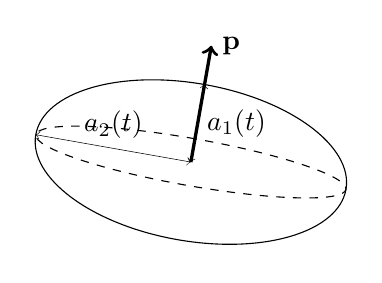
\begin{tikzpicture}[rotate=80]
        \draw(0,0) ellipse (1 cm and 2 cm);
        \draw[dashed](0,0) ellipse (0.3 cm and 2 cm);
        \draw[<->,very thin](0,0) --++ (1,0)node[midway,right]{$a_1(t)$};
        \draw[->,very thick](0,0) --++ (1.5,0)node[right]{$\textbf{p}$};
        \draw[<->,very thin](0,0) --++ (0,2)node[midway,above]{$a_2(t)$};
    \end{tikzpicture}
    \hfill
    \caption{Scheme of an  oblate spheroid oriented along the unit vector \textbf{p} with $a_1(t)$ and $a_2(t)$ the length of the semi axes of the spheroid.
    Note that when the drop is spherical we have $a_1=a_2=a$}
    \label{fig:scheme_spheroid}
\end{figure}
This shape might be described completely by the second moment of mass, $\textbf{M}_\alpha$.
In this context, each eigenvalue of the second moment of mass tensor is proportional to square semi axes of the particle. 
Indeed, by direct integration over the spheroidal particle volume we may find :
\begin{equation*}
    \textbf{M}_\alpha
    = \frac{m_\alpha a^2}{5}\left[
        \left(\frac{a_1}{a}\right)^2\textbf{pp}
        + \left(\frac{a_2}{a}\right)^2 (\textbf{I} - \textbf{pp}),
    \right] 
\end{equation*}
Additionally, note that due to the volume conservation condition we have : $ a_2^2 a_1 = a^3$. 
This means that : $M_1 = M_2^{-2}$, where the $M_i$ are the eigenvalues of the dimensionless tensor $\frac{m_\alpha a^2}{5}\textbf{M}_\alpha^* = \textbf{M}_\alpha$. 
Note that if we consider small deformations, meaning $M_1 - 1 \ll 1$ we have $M_1  = M_2^{-2} = 1 - 2 (M_2 - 1) + \mathcal{O}((M_2 -1)^2)$. 
Consequently, for small deformation the trace of the second moment of mass tensor reads :  $\frac{1}{3}\textbf{I}:\textbf{M}_\alpha = M_1 + 2M_2 = 1 - 2M_2 + 2M_2 = 1$. 
Therefore in the limit of small deformation the droplet shape is completely determined by one scalar value $M_1$ or $M_2$, and the orientation tensor $\textbf{p}$. 

Additionally, with this definition we can introduce the distance function  $\FF_\alpha$. 
It reads, 
\begin{equation*}
    \FF_\alpha(\textbf{x},t) = \textbf{rr}:\textbf{M}_\alpha^* -a^2.  
    \label{eq:distance_function}
\end{equation*}
The point on the surface of the particle are defined through $\FF_\alpha(\textbf{x}_I,t) = 0$. 
Being able to define the droplet's shape in such a rigorous way will find its use in the calculation of the surface tension stress. 
Using these definition makes the dimensionless  second moment of mass the same as the Cauchy green deformation tensor. 

\subsubsection*{The droplet's internal velocity}


We know that an isolated droplet in creeping flow with translating motion exhibit internal motion known as Hill vortexes, see \ref{fig:flowlines} (b). 
For a drop immersed in an unbounded linear flow, still in stokes flows, we can derive an analytical solution such that $\textbf{w}_2^0 \sim \textbf{rrr}$, see \ref{fig:flowlines} (a). 
If slightly more inertial effects are present one might find that the internal motion are close to hill's vortexes but with an overall oblate spheroidal shape, see \ref{fig:flowlines} (c). 
In these cases the droplet's internal velocity fields is a steady solution.
Nevertheless, for a droplet to go from case (b) to case (c) a deformation must occur. 

To account for this deformation in our case we assume that the secondary velocity field that is responsible for the deformation is purely a linear function of the position. 
The internal velocity field of a particle under homogeneous linear deformation can be described as such, $\textbf{w}_2^0 = \bm\Gamma_\alpha \cdot \textbf{r}$. 
We have introduced, $\bm\Gamma_\alpha$, the mean velocity gradient inside the particle, which symmetric part : $\textbf{E}_\alpha$, represents the rate of strain, and skew symmetric part : $\bm\Omega_\alpha$, represents the angular velocity. 

\begin{figure*}
    \centering
    \begin{tikzpicture}
        \node (img3) at (0.6\textwidth,0) {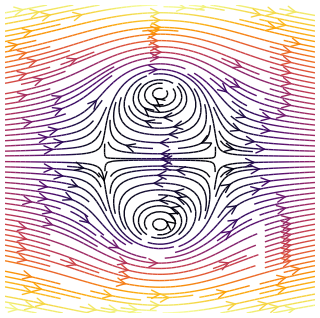
\includegraphics[width=0.3\textwidth,angle=270]{image/Rising_def_Stokes.png}};
        \node (img2) at (0.3\textwidth,0) {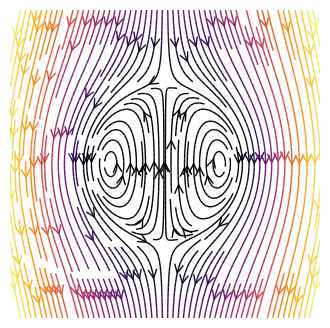
\includegraphics[width=0.3\textwidth]{image/Rising_Stokes.png}};
        % \draw (0.45\textwidth,0)node{$\rightarrow$};
        % \draw (0.45\textwidth,0.4cm)node{$\bm\Gamma_\alpha\cdot \textbf{r}$};
        \node (img1) at (0.0\textwidth,0) {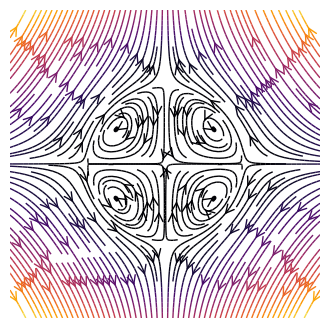
\includegraphics[width=0.3\textwidth]{image/Shear_Stokes.png}};
        \draw (img3.south)node{(c)};
        \draw (img2.south)node{(b)};
        \draw (img1.south)node{(a)};
    \end{tikzpicture}
    \caption{Three examples of steady state flow lines plots of an isolated droplet immersed into a viscous fluid. 
    (a) Rising sphere in uniform stokes flow (analytical solution in \ref{ap:Translating_sphere}). 
    (b) Fixed droplet in extensional flow (analytical solution in \ref{ap:Translating_sphere}).
    (c) Deformed droplet in rising motion (analytical solution of \citet{taylor1964deformation}). }
    \label{fig:flowlines}
\end{figure*}
To summarize, we assume that the inner velocity field of the drop can be decomposed into two distinct part. 
The first one is the steady state component, examples are : hill's vortex for spherical and oblate spheroidal drop in steady linear motion, the inner velocity field of a drop in steady linear flows, and so on. 
The second contribution is the inner velocity fields that alter the drop's shape, this field is assumed linear with the position and homogeneous, that is $\bm\Gamma\cdot \textbf{r}$. 
Adopting these definitions, the particle internal velocity is written, 
\begin{equation}
    \textbf{w}_{2,i}^0(\textbf{x}_\alpha)
    = \bm\Gamma_{\alpha,ik}(t) \cdot \textbf{r}_k
    + \textbf{w}^{s}_{2,i}(t,\textbf{r})
    =\bm{\Omega}_{\alpha,ik}\cdot \textbf{r}_k
    + \textbf{E}_{\alpha,ik} \cdot \textbf{r}_k
    + \textbf{w}^{s}_{2,i}(t,\textbf{r})
    \label{eq:def_vel}
\end{equation}
Where we introduced the vector $\textbf{w}^{s}_2(t,\textbf{r}) =\textbf{w}^{0}_{2,i}(t,\textbf{r})  - \bm\Gamma_{\alpha,ik}(t) \cdot \textbf{r}_k$ which represents all the internal motions that does not alter the drop's shape. 

An important consequence of this definition is that the integral on the RHS of \ref{eq:dt_S_alpha} is null when $\textbf{w}_{2,i}^0 = \textbf{w}_{2,i}^s$. 
This can be shown by re writting the second moment of mass equation with the use of the velocity decomposition.
This yields,
\begin{equation*}
    \ddt \textbf{M}_{\alpha,ik}
    = 
    \textbf{M}_{\alpha,ik} \cdot \bm\Gamma_{\alpha,kj}
    +  \bm\Gamma_{\alpha,ki} \cdot \textbf{M}_{\alpha,jk}
    +
    \intO{ 
        \textbf{w}_{2,i}^s\textbf{r}_j
        + \textbf{r}_i\textbf{w}_{2,j}^s
    }
\end{equation*}
In the cases where $\bm\Gamma = 0$, the droplet shape remains steady, in this case $\ddt \textbf{M}_\alpha = 0$ and $\intO{\textbf{w}^{s}_{2,i} \textbf{r}_j + \textbf{r}_i \textbf{w}_{2,i}^s} = 0$. 
In the case where $\bm\Gamma \neq 0$ the droplets deform according to the linear velocity fields $\bm\Gamma\cdot \textbf{r}$.
Since we assumed that no other source of deformation are present than the latter, we must have $\intO{\textbf{w}^{s}_{2,i} \textbf{r}_j + \textbf{r}_i \textbf{w}_{2,i}^s} = 0$ so that $\textbf{w}^{s}_{2,i} $ doesn't contribute to the deformation nor the rotation.
This, means that $\textbf{w}^{s}_{2,i}$ is a velocity fields determined in  part by the instantaneous shape of the droplet and its , that does not alter the shape of the drop. 
Additionally, the angular momentum is assumed to be entirely described by $\textbf{M}_\alpha \cdot \bm\Omega_\alpha$ meaning that, $\textbf{r} \textbf{w}_{2}^s$ plays no role at all in the total particle's moment of momentum.
This type of velocity fields is encountered in linear skew symmetric flows where the rotation is homogeneous and follow the carrier fluid vorticity. 
Anyhow, this velocity decomposition has the plaisent property that $\textbf{P}_\alpha = \bm\Gamma \cdot \textbf{M}_\alpha + \intO{\textbf{w}^{s}_{2,i} \textbf{r}_j} =  \bm\Gamma \cdot \textbf{M}_\alpha $ at all time, which will simplify the equaitons of motions. 

Now some constrain should apply on the tensor $\textbf{E}_\alpha$.
Indeed, the mass conservation inside the particle \ref{eq:dt_rho} impose $\div \textbf{u}_2^0 = \textbf{E}_\alpha : \textbf{I}= 0$, where it is assumed that $\div \textbf{w}_2^s =0$. 
Also, note that to preserve the spheroidal shape of the particle we must assume that the particle's rate of strain principal direction is the same as the droplet's shape principal axis. 
In other worlds, $\textbf{E}_\alpha$ must have the same eigenbasis as $\textbf{M}_\alpha$. 
Making up with these two constrain leads to the expression : $\textbf{E}_\alpha = -2 E_2 \textbf{pp} + E_2 (\textbf{I}- \textbf{pp})$, where $E_2$ is the second eigenvalue of $\textbf{E}_\alpha$. 


As it is demonstrated in \ref{ap:Translating_sphere} the internal motion of an isolated spherical drop, such as the one in \ref{eq:def_vel}, is entirely determined  from $\textbf{u}_1$,$\grad\textbf{u}_1$,$\textbf{u}_\alpha$ and so on. 
Therefore, it is reasonable to think that in a more general case, $\textbf{w}_2^s$ might be entirely determined by the carrier fluid and particles' properties, namely, $\textbf{u}_\alpha$ $\textbf{M}_\alpha$, $\textbf{u}_1$ $\grad\textbf{u}_1$ and for non-dilute flows we might have $\phi_2$ or more complicated functions. 
Thus, from now on we consider that the internal velocity $\textbf{w}^{s}_2(t,\textbf{r})$ is not part of the particle' unknown, but rather is a closure term. 
Consequently, in this problem a single droplet is described exhaustively by, $\textbf{x}_\alpha, \textbf{u}_\alpha, \textbf{M}_\alpha$ and $\bm\Gamma_\alpha$. 
This requires two additional equations one for $\textbf{M}_\alpha$ and another for $\bm\Gamma_\alpha$. 

\subsubsection*{The conservation equations}

The integrals appearing in \ref{eq:dt_M_alpha} and \ref{eq:dt_P_alpha} can be reformulated using the previous decomposition of the internal velocity field, and it reads, 
\begin{align}
    \intO{(\textbf{rw}_ 2^0 )_{ij}+ (\textbf{w}_2^0 \textbf{r})_{ij}} 
    = \textbf{M}_{\alpha,ik} \cdot \bm\Gamma_{\alpha,jk}
        +  \bm\Gamma_{\alpha,ik} \cdot \textbf{M}_{\alpha,jk}
    \\
    \intO{\rho_2 \textbf{w}_{2,i}^0\textbf{w}_{2,j}^0}
    = \bm\Gamma_{\alpha,jl}\bm\Gamma_{\alpha,ik} \textbf{M}_{\alpha,kl}  
        +\intO{\rho_2 \textbf{w}_{2,i}^s\textbf{w}_{2,j}^s}
    \\
    \intO{\bm\sigma_{2,ij}^0}
    =
    2 \mu_2 v_\alpha \textbf{E}_{\alpha,ij}
    - \intO{p_2^0} \textbf{I}_{ij}
    + \mu_2 \intS{(\textbf{n}_i \textbf{w}_{2,j}^s + \textbf{n}_j \textbf{w}_{2,i}^s)}
    \\
    \intS{\bm\sigma_{I,ij}^0}
    = \frac{\gamma v_\alpha }{a} \left[
        2\textbf{I}_{ij} 
        - \frac{4  }{5} (\textbf{M}_{\alpha,ij}^* - \textbf{I}_{\alpha,ij})
    \right]
    +\mathcal(O)((\textbf{M}_\alpha-\textbf{I})^2)\\
    % s_\alpha 
    % = 4\pi a^2 (1+\frac{\textbf{M}:\textbf{M}}{15})
\end{align}
The reformulation of the moment of momentum have already been treated above. 
The surface tension stress has been derived in the limit of small deformation. 
Note that our formula agree with the one derived by \citet{lhuillier1987phenomenology}. 
The detailed calculation of the surface tension stress tensor is given in appendix. 
We provide the exact results as well as the Taylor expansion of this formula for small deformation. 

Injecting these formulas inside \ref{eq:dt_M_alpha} and \ref{eq:dt_P_alpha} yields an equation for the deformation and the rate of strain of the drop. 
If we separate the skew-symmetric, symmetric and trace of the moment of momentum equation we obtain and equation for $\bm\Omega_\alpha$ and one fer  $\textbf E_\alpha$, namely,
\begin{align*}
    % \ddt \textbf{pp}_{\alpha,ij}
    % = \textbf{pp}_{\alpha,ik} \cdot \bm\Omega_{\alpha,jk}
    % +  \bm\Omega_{\alpha,ik} \cdot \textbf{pp}_{\alpha,jk}\\
    \ddt \textbf{M}_{\alpha,ij}
    = \textbf{M}_{\alpha,ik} \cdot \bm\Gamma_{\alpha,jk}
    +  \bm\Gamma_{\alpha,ik} \cdot \textbf{M}_{\alpha,jk}\\
    \ddt (\textbf{I}_{\alpha,ik}\bm\omega_{\alpha,k} )
    = 
    \intS{(\textbf{r}\times\bm\sigma_1^0\cdot \textbf{n})_i} \\
    \frac{1}{2}\ddt^2 \textbf{M}_{\alpha,ij}
    -  \bm\Gamma_{\alpha,jl}\bm\Gamma_{\alpha,ik} \textbf{M}_{\alpha,kl}  
    + \mu_2 v_\alpha 2\textbf{E}_{\alpha,ij}
    + \frac{\gamma v_\alpha }{a} \left[
    2\textbf{I}_{ij} 
    - \frac{4 }{5} (\textbf{M}_{\alpha,ij}^* - \textbf{I}_{\alpha,ij})
    \right]\\
    = 
    \frac{1}{2}\intS{(\textbf{r}\bm\sigma_1^0 + \bm\sigma_1^0\textbf{r})\cdot \textbf{n}} 
    + \intO{\rho_2 \textbf{w}_{2,i}^s\textbf{w}_{2,j}^s}
    + \intO{p_2^0} \textbf{I}_{ij}
    - \mu_2 \intS{(\textbf{n}_i \textbf{w}_{2,j}^s + \textbf{n}_j \textbf{w}_{2,i}^s)}\\
    % \frac{1}{2}\ddt^2 \textbf{M}_{\alpha,mm}
    % -  \bm\Gamma_{\alpha,ml}\bm\Gamma_{\alpha,mk} \textbf{M}_{\alpha,kl}  
    % + \frac{\gamma v_\alpha }{a} 
    % \left[
    % 2\textbf{I}_{mm} 
    % % - \frac{4 }{5 } (\textbf{M}_{\alpha,mm}^* - \textbf{I}_{\alpha,mm})
    % \right]
    % = 
    % \intS{\textbf{r}_m\cdot\bm\sigma_{1,mk}^0\cdot \textbf{n}_k} 
    % + \intO{\rho_2 \textbf{w}_{2,m}^s\cdot \textbf{w}_{2,m}^s}
    % + \intO{p_2^0} \textbf{I}_{mm}
\end{align*}
The second moment of mass \ref{eq:dt_Cs}, is consistent with the equation found by \citet{goddard1967nonlinear} and \citet{lhuillier1987phenomenology}. 
Following, \citet{goddard1967nonlinear}  terminology, the left-hand side of \ref{eq:dt_Cs} is referred as the \textit{convected} derivative of $\textbf{M}^*_\alpha$. 
Therefore, the \textit{convected} derivative of $\textbf{M}_\alpha$ is equal to the rate of strain of the particle. 
The skew-symmetric part of the first moment of momentum \ref{eq:dt2_C}, it is basically the angular momentum balance of a non-spherical object. 
The right-hands side accounting for the external torque contribution. 
The symmetric part however has the form of a non-linear forced harmonic oscillatory equation for the droplet deformation. 
Indeed, the first groups of terms on the left-hand side represent the inertial contribution of the droplet internal fluid. 
It is made of a second order derivative plus non-linear terms in $\bm\Gamma_\alpha$. 
The second groups of terms is internal viscous contribution that arise directly from the definition of the stress \ref{eq:sigma_2_def}. 
It vanishes for small viscosity ration and is linear in the first derivative of $\textbf{M}_\alpha$. 
The last term on the left-hand side is the elastic response from the interface which is negligible for high capillary number $Ca \to \infty$. 
Then on right-hand side of the equation we find the first moment of surface force, $\intS{(\textbf{r}\bm\sigma_1^0+ \bm\sigma_1^0\textbf{r})\cdot \textbf{n}}^*$ which has an unknown expression at this stage. 
\ref{eq:dt2_C} might be regarded as a second order harmonic equation with non-linear contributions. 
However, the unknown integrals $\intO{\rho_2 \textbf{w}_{2,i}^s\textbf{w}_{2,j}^s},
\intS{(\textbf{n}_i \textbf{w}_{2,j}^s + \textbf{n}_j \textbf{w}_{2,i}^s)}$ and $\intS{(\textbf{r}\bm\sigma_1^0+ \bm\sigma_1^0\textbf{r})\cdot \textbf{n}}^*$ are in general function of the shape of the particle so on $\textbf{M}_\alpha$ and its higher derivatives of $\textbf{M}_\alpha$.
These terms have to be seen as forcing terms. 
Therefore, at this stage it is impossible to predict the nature of the harmonic regime followed by the droplet. 
To conclude on this matter one must find an expression for all this closure as well as determinate the impact of the non-linear terms.



We now focus on the rate of strain equation. 
To better understand this equation we introduce the following dimensionless groups, 
\begin{align*}
    \intO{\rho_2 \textbf{w}_{2,i}^0\textbf{w}_{2,j}^0}
    \sim \frac{m_\alpha a^2}{\tau_u^2} \textbf{F}_{ww}^*
    \\
    - \intO{p_2^0\textbf{I}}
    + \mu_2 \intS{(\textbf{n}_i \textbf{w}_{2,j}^s + \textbf{n}_j \textbf{w}_{2,i}^s)}
    \sim \frac{v_\alpha \mu_2}{\tau_u} \textbf{F}_{e}^*
    \\
    \intS{\textbf r \bm\sigma_1^0 \cdot \textbf{n}}
    \sim 
    \frac{v_\alpha \mu_1}{\tau_u} \textbf{F}_{\sigma}^*
\end{align*} 
where we have assumed that the internal and external stress contribution followed a viscous scaling. 
The time $\tau_u$ represent the external solicitation time-scale. 
Which is in opposition to the droplets rate of strain and rotation time scale such that $\bm\Gamma = 1/\tau \bm\Gamma^*$. 
\begin{align*}
    \frac{\zeta Re}{5}\left[
        \beta^2 \frac{1}{2}\ddt^2 \textbf{M}_{\alpha,ij}
    -   \beta^2 \bm\Gamma_{\alpha,jl}\bm\Gamma_{\alpha,ik} \textbf{M}_{\alpha,kl}  
    - \textbf{F}_{ww}^*
    \right]
    + \lambda  \left[
        \beta 2\textbf{E}_{\alpha,ij}
    +  \textbf{F}_\sigma^*
    \right]
    + \frac{1}{Ca} \left[
    2\textbf{I}_{ij} 
    - \frac{4  }{5} (\textbf{M}_{\alpha,ij}^* - \textbf{I}_{\alpha,ij})
    \right]
    = 
    \frac{1}{2}
    \textbf{F}_{\sigma_1}^*
    % \intS{(\textbf{r}\bm\sigma_1^0 + \bm\sigma_1^0\textbf{r})\cdot \textbf{n}} 
    % + \intO{p_2^0} \textbf{I}_{ij}
\end{align*}
where we have defined the following dimensionless groups : 
\begin{align*}
    \beta = \frac{\tau_u}{\tau}
    && \zeta = \rho_2 /\rho_1
    && \lambda = \mu_1/\mu_2 
    && Re = \frac{\rho_1 a^2 }{ \mu_1 \tau_u}
    && Ca = \frac{a \mu_1}{\gamma \tau_u}
\end{align*}

We now examine the specific case studied by \citet{lamb1924hydrodynamics} where he considered no external contribution around the particle nor rotational motion.
Also, it is considered that the deformation within the particle are linear and small. 
Keeping only the trace of this equation yields the low deformation system of equation :
\begin{align*}
    \ddt \textbf{M}_{\alpha,ij} = \textbf{E}_{\alpha,ij}\\
    \frac{\zeta Re}{5}
        \beta^2 \frac{1}{2}\ddt^2 \textbf{M}_{\alpha,ij}
    % -   \beta^2 \bm\Gamma_{\alpha,jl}\bm\Gamma_{\alpha,ik} \textbf{M}_{\alpha,kl}  
    % - \textbf{F}_{ww}^*
    % \right]
    + \lambda 
        \beta 2\textbf{E}_{\alpha,ij}
    % +  \textbf{F}_\sigma^*
    % \right]
    - \frac{1}{Ca} 
     \frac{4  }{5} (\textbf{M}_{\alpha,ij}^* - \textbf{I}_{\alpha,ij})
    = 0
    % \frac{1}{2}
    % \textbf{F}_{\sigma_1}^*
    % \intS{(\textbf{r}\bm\sigma_1^0 + \bm\sigma_1^0\textbf{r})\cdot \textbf{n}} 
    % + \intO{p_2^0} \textbf{I}_{ij}
\end{align*}
Notice that this is a second order oscillatory equation. 
This is equivalent to  \citet{lamb1924hydrodynamics}. 
Therefore our model is somewhat more general. 

Lastly, as it will be usefull for latter let consider the cases wheer the timescale of the flow is much smaller that the one of the particle rate of strain, in this case $\beta \ll 1$. 
Making use of this fact makes the moment of momentum equation as, 
\begin{align*}
    - \frac{\zeta Re}{5}
     \textbf{F}_{ww}^*
    + \lambda  
    \textbf{F}_\sigma^*
    + \frac{1}{Ca} \left[
    2\textbf{I}_{ij} 
    + \frac{4  }{5} (\textbf{M}_{\alpha,ij}^* - \textbf{I}_{\alpha,ij})
    \right]
    = 
    \frac{1}{2}
    \textbf{F}_{\sigma_1}^*
    % \intS{(\textbf{r}\bm\sigma_1^0 + \bm\sigma_1^0\textbf{r})\cdot \textbf{n}} 
    % + \intO{p_2^0} \textbf{I}_{ij}
\end{align*}
This is the steady state equilibrium equation of the first moment of force. 
If the capillary number is low enough the last term  completely balance the external stress. 

% 
\subsection{From Lagrangian to Eulerian fields}

Up to this point, we have described the dispersed phase within a Lagrangian framework.
However, to be consistent with the Eulerian conservation equations used to describe the continuous phase, we need to extend the Lagrangian equations to an Eulerian models. 
In order to achieve this, we introduce the function $\delta_\alpha$, which is defined as follows, 
\begin{align}
    \delta_\alpha(\textbf{x},t) = \delta(\textbf{x}-\textbf{x}_\alpha(t,\FF)).
    \label{eq:delta_alpha}
\end{align}
where $\delta$ is the Dirac delta function.
Note that we explicitly note $\textbf{x}_\alpha(t,\FF)$ since the posiiton of the particle $\alpha$ is function of time and of the flow configuration $\FF$.
In the sens of generalized functions, the partial time derivative, $\pddt \delta_\alpha(\textbf{x},t,\FF) =  \frac{\partial \textbf{x}_\alpha}{\partial t} \cdot \grad_{\textbf{x}_\alpha} \delta_\alpha$ can be re-written into the following expression, 
\begin{equation}
    \pddt \delta_\alpha
    + \div (\textbf{u}_\alpha  \delta_\alpha)
    =0,
    \label{eq:dt_delta_alpha}
\end{equation}
where we used the identity, $\grad_{\textbf{x}_\alpha} \delta_\alpha = -\grad \delta_\alpha$ and the fact that $\textbf{u}_\alpha(t;\FF)$ is not a function of $\textbf{x}$. 
Additionally, it should be noted that \ref{eq:dt_delta_alpha} is not applicable if changes in topology, such as break up or coalescence events, occur.
In such cases it is possible, as it is done in population balance equations, to include a source term on the RHS of \ref{eq:dt_delta_alpha} to account for particle birth or death. 
Multiplying each Lagrangian quantities by $\delta_\alpha$ yields the \textit{particle field} of a quantity $q_\alpha$, denoted as $q_\alpha(t)\delta_\alpha(\textbf{x},t)$, which is defined throughout space and time.
Likewise, for any derivative of Lagrangian quantities, such as $\ddt q_\alpha$, we define its corresponding Eulerian field by Multiplying $\ddt q_\alpha$ with $\delta_\alpha$ and show that :
\begin{equation}
    \delta_\alpha \ddt q_\alpha
    = \pddt (\delta_\alpha q_\alpha)
    + \div (\delta_\alpha q_\alpha \textbf{u}_\alpha)
    \label{eq:dt_delta_alpha_q_alpha}
\end{equation}
where we have utilized the fact that $q_\alpha(t)$ and $\textbf{u}_\alpha(t)$ are solely functions of time, and we made use of \ref{eq:dt_delta_alpha}.
Additionally, let's consider a volume containing $N$ particles.
We can then define the particle-field of a given quantity $q_\alpha$ as the sum of all the independent field, i.e. $\sum_{\alpha=0}^N \delta_\alpha q_\alpha$.
Notice that \ref{eq:dt_delta_alpha_q_alpha} remains valid for a sum of fields since derivative operators are linear.
To simplify the notations, we consider implicitly the summation over all particles included in $\Omega$ whenever a Lagrangian field denoted by $\delta_\alpha (\ldots)$ is present.

Multiplying \ref{eq:dt_q_alpha_tot} and \ref{eq:dt_Q_alpha_tot} by $\delta_\alpha$, summing over all particles, and by considering \ref{eq:dt_delta_alpha_q_alpha}, it is straightforward to show that,
\begin{equation}
    \pddt (\delta_\alpha  q_\alpha^\text{tot})
    + \div (\delta_\alpha\textbf{u}_\alpha q_\alpha^\text{tot})
    = \delta_\alpha\intO{ s_2^0 }
    + \delta_\alpha\intS{ s_I^0 }
    + \delta_\alpha\intS{ \left[\mathbf{\Phi}_1^0 + f_1^0 (\textbf{u}_I^0-\textbf{u}_1^0) \right] \cdot \textbf{n}_2 },
    \label{eq:dt_dq_alpha_tot}
\end{equation}
\begin{multline}
    \pddt (\delta_\alpha  \mathcal{Q}_\alpha^\text{tot})
    + \div (\delta_\alpha\textbf{u}_\alpha \mathcal{Q}_\alpha^\text{tot})
    = \delta_\alpha\intO{ \left(
        \textbf{r} s_2^0         
        + f_2^0  \textbf{w}_2^0 
        - \mathbf{\Phi}_2^0
    \right) }\\
    + \delta_\alpha\intS{ \left(
        \textbf{r}s_I^0
        + f_I^0 \textbf{w}_I^0
        - \mathbf{\Phi}_{||I}^0
    \right) }
    + \delta_\alpha\intS{ \textbf{r} \left[
        \mathbf{\Phi}_1^0
        + f_1^0 (\textbf{u}_I^0-\textbf{u}_1^0)
    \right]\cdot \textbf{n}_2  }.
    \label{eq:dt_dQ_alpha_tot}
\end{multline}
Similar consideration can be applied to the higher order moments equations derived in \ref{ap:moment_derivative}.

At this stage, we obtained two sets of equations that can be used to describe the dispersed phase. 
The first set of equations is the global conservation laws, i.e. \ref{eq:dt_chi_k_f_k} with for $k=2$ and \ref{eq:dt_delta_I_f_I}. 
The other is the particle-fields equations, such as \ref{eq:dt_dq_alpha_tot} and potentially the higher moments equations.
Therefore, some comments are in order regarding the differences and compatibility of these two sets of equations.
Solving \ref{eq:dt_dq_alpha_tot} ideally provides us with a field $\delta_\alpha(q_\alpha+q_{I\alpha})$ which contains the Lagrangian properties $q_\alpha+q_{I\alpha}$.
Thus, it corresponds to the volume and surface integral of $f_2^0$ and $f_I^0$ on $\Omega_\alpha$ and $\Sigma_\alpha$ respectively.
While, in \ref{eq:dt_chi_k_f_k} we solve the equation for the complete field $f_2^0$ defined inside the domains $\Omega_\alpha$.  
Thus, from  \ref{eq:dt_f_k} to \ref{eq:avg_dt_dq_alpha_tot} we lose the detailed description of $f_2^0$ within the particles' domain.
Indeed, with \ref{eq:avg_dt_dq_alpha_tot}, we recover solely the integrated value of $f_2^0$ over the particles' volume and surface. 
Therefore, \ref{eq:dt_dq_alpha_tot} can be though as averaged equations of \ref{eq:dt_chi_k_f_k} and \ref{eq:dt_delta_I_f_I} since we recover only the integrated properties of each particle. 
It is important to understand that in this sense, the passage from \ref{eq:dt_chi_k_f_k} and \ref{eq:dt_delta_I_f_I} to \ref{eq:dt_dq_alpha_tot} is an average operation carried out on the particles' volume and surface.
Likewise, \ref{eq:dt_dQ_alpha_tot} is an equation for the first moment of the distribution of $f_2^0$ and $f_I^0$ within the particle's volume and surface.

% Note that this is different to the usual averaged technics that refer to the ones used to derive the classic averaged models such as in \citet{jackson1997locally} and \citet{zhang1994averaged}.
% which are the subject of the following section. 


\section{The hybrid model}
\subsection{Averaged particle phase equation}
\subsubsection{First order simple laws}
\subsubsection{Orientation / rotations law (get from appendix) order simple laws}
\tb{These are valid for solid particles only the closures changes }
\subsubsection{Deformation laws in the local reference frame}

\tb{maybe useless in averaged form but whatever}
\subsection{Averaged continuous phase equation}

\subsubsection{Fluid phase momentum and mass equations}
\subsection{
    The finite inertial effect on the Rheology of deformable droplets' emulsion.
    % phase relative velocity on the rheology of mono-disperse dilute emulsion of deformable droplets
    }

In this section we make use of the \textit{hybrid model} to demonstrate how to derive the minimal set of equation intended to model deformable droplets in a buoyant emulsion. 

Preceding studies have intended to model the rheology of dilute emulsion of neutrally buoyant deformable droplets, in stokes regime \citep{goddard1967nonlinear,lhuillier1987phenomenology,maffettone1998equation}.
More recently, researcher have been trying to include inertial effect in these models \citet{raja2010inertial,mwasame2018macroscopic}. 
However, these studies have been conducted in the objective of determining the equivalent shear stress of a neutrally buoyant suspension, i.e. they study the mean stress $\bm{\sigma}$ in terms of the imposed flow gradient $\textbf{e}$ for a given microstructure. 
Therefore, to the knowledge of the author all preceding study disregards the impact of relative motion on the suspension rheology. 

In this application, we focus on the Rheological behavior of an inertial emulsion of spheroidal deformable rising droplets with a finite phase relative velocity. 
Thus, we seek for an expression of the bulk stress $\bm{\sigma}$, in terms of the mean relative motions $\textbf{u}_{pf}$. 
As the purpose is to point out the effect of the translational motions on the stress, we consider that there is no mean shear within the emulsion, i.e. $\textbf{e} = 0$. 
Nevertheless, we want to be clear on the facts that of mean shear are present its contribution to the stress is certainly non-negligible. 

\subsubsection*{Determination of the shape and strain based on \citet{taylor1964deformation} theoretical results}

\begin{itemize}
    \item In the capillary dominant regime stresslet = shape and this is it 
    \item Iso-viscous low density bubbles (that might not existe) permitt to neglect these
    \item (1) In the prvious section we proposed an equation for shape and rate of strain of the particles
    \item (2) In taylor they provide direct closure for the shape in steady state regime, no need for an equation anymore
    \item (3) considering this relation we can in fact re formulate the  bulk stress in term of this shape direct closure
    \item (4) Also the fluid phase stress can be written as ww -p etc... In any case we now that the functional form of the stress will be proportional to $u u $ 
    \item (5) In inertial regime the stresslet will also be present 
    \item (6) Major  conclusion is that the stesslet is also function of uu and that is far from being negligible. 
\end{itemize}




In \citet{taylor1964deformation} they derive the shape and the drag force of a translating droplet at $\textbf{O}(Re^2)$ in a steady state situation. 
The derivation is done in the low but finite $Re$ and $Ca$. 
The dimensionless radius of the droplets can be express in the polar coordinate reference frame of the drop as, 
\begin{equation*}
    \frac{R_\text{taylor}(\theta)}{a} = 1 - \beta \textit{We} P_2(\cos\theta)
    + \mathcal{O}(We^2)
    \label{eq:taylor_solution}
\end{equation*}
where $Re = |\textbf{u}_{pf}| a /\nu_1$ with $|\textbf{u}_{pf}|$ the phase relative velocity, $P_2(\cos\theta)$ is the Legendre polynomial of degree two and $\kappa$ is a coefficient related to physical parameters given in \citet{taylor1964deformation}.  
This solution need to satisfy $\kappa Re \ll 1$ and $Re \ll 1$ to be valid. 
It is then possible to reformulate $\textbf{C}_\alpha$ in terms of the relative velocity $\textbf{u}_{pf}$, it yields, 
\begin{equation}
    \textbf{C}_\alpha =  \frac{ \rho_1 a \beta}{\gamma} \left[
        -  3
        (\textbf{u}_{\alpha f}\textbf{u}_{\alpha f})
        +   (\textbf{u}_{\alpha f}\cdot\textbf{u}_{\alpha f})\textbf{I}
    \right]
    % +\textbf{u}_{\alpha f}\cdot\textbf{u}_{\alpha f}\left(\frac{ \beta \rho_1 a}{\gamma}\right)^2
    % \left[
    %     \frac{3}{4}
    %     \textbf{u}_{p f}\textbf{u}_{p f}
    %     +
    %     \frac{1}{4}
    %     (\textbf{u}_{p f}\cdot\textbf{u}_{p f})
    %     \textbf{I}
    % \right]
    + \mathcal{O}(\textit{We}^2)
\end{equation}
where we have neglected terms of $\mathcal{O}(\textit{We}^2)$ as at this order the droplet shape isn't spheroidal anymore \citet{taylor1964deformation}. 
We now apply an average procedure on $\textbf{C}_\alpha$, and by noticing that, $\pavg{\textbf{u}_{\alpha f}\textbf{u}_{\alpha f}} = \textbf{u}_{pf}\textbf{u}_{pf} + \pavg{\textbf{u}_\alpha'\textbf{u}_\alpha'}$ we obtain the following expression 
for the averaged shape of the droplets, 
\begin{equation*}
    \textbf{C}_p  =  \frac{ \rho_1 a \beta}{\gamma} \left[
        -  3
        (\textbf{u}_{p f}\textbf{u}_{p f} + \avg{\textbf{u}_\alpha'\textbf{u}_\alpha'})
        +   (\textbf{u}_{p f}\cdot\textbf{u}_{p f}+2k_p)\textbf{I}
    \right]
    + \mathcal{O}(\textit{We}^2)
\end{equation*}
Under these quite restrictive assumption we have shown that the shape of the particle $\textbf{C}_p$ can be expressed with the relative phase velocity and particles fluctuating terms. 

Now that we have determined the mean deformation tensor within our suspension we use the second moment of mass equation to determine the strain rate and angular velocities of the particles. 
Averaging \ref{eq:dt_Cs} directly gives, 
\begin{equation}
    n_p 
    (\bm\Gamma_{p,ij}
    +  \bm\Gamma_{p,ji})
    + \textbf{C}_{p,ik}^* \cdot \bm\Gamma_{p,kj}
    + \bm\Gamma_{p,ki}^* \cdot \textbf{C}_{p,jk},
    = 
    % \pavg{\ddt \textbf{C}_{p,ij}^*}
    \pddt (n_p \textbf{C}_{p,ij}^*)
    + \div(n_p \textbf{u}_p \textbf{C}_{p,ij}^*)
\end{equation}
The fluctuations terms between the particles shape, $\textbf{C}_\alpha^*$ and the particle velocity $\textbf{u}_\alpha$, will in fact be fluctuations terms of third order in the particle velocity distribution.
Indeed, using \ref{C_def_with_u} eventually leads to $\pavg{\textbf{C}'_\alpha \textbf{u}_\alpha'} \sim \pavg{\textbf{u}_\alpha'\textbf{u}_\alpha' \textbf{u}_\alpha'}$. 
Regarding the rate of strain particle's velocity covariance we suppose that it is null as the rate of strain isn't a priori correlated with the latter property. 
Anyhow, at this stage of advancement we must suppose these terms negligible. 

\subsubsection*{Expression of the fluid phase equivalent stress}

We have seen that for spherical particle the relative velocity $\textbf{u}_{fp}$ is involved in the momentum equation through its presence via the drag force term and the second moment of the surface stress only.  
In this case we have shown that the averaged stresslet, is also a function of the relative velocity due to the inertial nature of the suspension. 

In the equivalent stress, the stress let contribution appear as, 

% Using \ref{eq:Stresslet_quasi_steay} 
% Therefore, the stress for the fluid phase can be re written, 
% \begin{align*}
%     \bm{\sigma}^\text{eq}_{1,ik} =
%     \rho_1\avg{\chi_1\textbf{u}_1'\textbf{u}_1'}_{ik} 
%     + p_1 \delta_{ik}
%     - 2 \mu_{Ein}(\phi_2) \textbf{e}\\
%     + \mu_{Rel}(Re) \left[\partial_k (\phi_2\textbf{u}_{fp,i}) + \partial_i (\phi_2\textbf{u}_{fp,k})\right]
%     + \lambda_\text{Rel}(Re)
%         \delta_{ik} \partial_l(\phi_2 u_{fp,l})
% \end{align*}
% where we have assumed that the second moment of the surface traction preserve its functional form but have an additional coefficient proportional to $Re$. 

% \tb{FOR BUBBLE WE CAN GIVES A CLEAR CONCLUSION # the stresslet is directly linked to the pressure + shape}
The expression for equivalent bulk stress might be written in the most general way as, 
\begin{align*}
    \bm{\sigma}^\text{eq}
    = \avg{\textbf{u}'\textbf{u}'}
    - p \textbf{I}
    + \mu_1 \textbf{e}
    + \mu_1 \phi_2 \textbf{e}_2 (\lambda - 1)
    +\phi_I \bm{\sigma}_I 
\end{align*}
The integral of the internal stress is quite complicated. 
If we discard internal stresses we found, 
\begin{align*}
    \bm{\sigma}^\text{eq}
    = \avg{\textbf{u}'\textbf{u}'} 
    - p_1 \textbf{I}
    + \mu_1 \textbf{e}
    + \frac{\phi_2 \gamma}{a} \left[
        2 \textbf{I}_{ij} - \frac{4}{5} \textbf{C}_{p,ij}^*
    \right]
\end{align*}
\tb{add all the terms and say it is neglected }
where the function is the integral of the stress in the expression of \citet{taylor1964deformation}. 
In the quasi steady hypothesis the ratio of viscosity must respect $\lambda \to 0$. 
However, we keep it there since it doesn't bring any simplifications to the expression of the bulk stress. 
The unknown function $f_{\bm\sigma}$ can be determined from the velocity fields solution of \citet{taylor1964deformation} by integrating the stress over the volume of the spheroidal droplet. 
The expression obtained is determined by the relative phase velocities $\textbf{u}_{\alpha f}$, and will add a contribution to the stress due to the steady state internal velocity and pressure flied of the drops. 
Note that it is possible to give a similar expression for carrier fluid phase stress. 
The only difference with the former is that in the carrier fluid phase stress the coefficient $(\lambda - 1)$ becomes $1$. 
% \subsubsection*{The expression of the carrier fluid stress}
% Regarding the fluid phase stressit 
% As before we assume a homogeneous suspension yielding a fluid phase stress similar to \ref{eq:sigma_eq_0} but without the term under the divergence operator. 
% Substituting the first moment of the particle by \ref{eq:dt} 
\begin{multline*}
    \bm{\sigma}^\text{eq}_1 = 
    \rho_1\avg{\chi_1\textbf{u}_1'\textbf{u}_1'} 
    + \phi_1 p_1 \textbf{I} 
    - \mu_1 \textbf{e} 
    + \frac{1}{2}\ddt^2 \textbf{M}_{\alpha,ij}
    -  \bm\Gamma_{\alpha,jl}\bm\Gamma_{\alpha,ik} \textbf{M}_{\alpha,kl}  
    + \mu_2 v_\alpha 2\textbf{E}_{\alpha,ij}\\
    + \frac{\gamma v_\alpha }{a} \left[
    2\textbf{I}_{ij} 
    - \frac{4 }{5} (\textbf{M}_{\alpha,ij}^* - \textbf{I}_{\alpha,ij})
    \right]\\
    - \intO{\rho_2 \textbf{w}_{2,i}^s\textbf{w}_{2,j}^s}
    - \intO{p_2^0} \textbf{I}_{ij}
    + (\mu_2 - \mu_1)\intS{(\textbf{n}_i \textbf{w}_{2,j}^s + \textbf{n}_j \textbf{w}_{2,i}^s)}
    \label{eq:Steady_state_bubble}
\end{multline*} 
% where $f_{\textbf{e}}$ is the integral of the strain rate within the drop from the solution of \citet{taylor1964deformation}. 
As mentioned for small particle deformation and quasi steady state we have,  
\begin{multline*}
    \bm{\sigma}^\text{eq}_1 = 
    \rho_1\avg{\chi_1\textbf{u}_1'\textbf{u}_1'} 
    + \phi_1 p_1 \textbf{I} 
    - \mu_1 \textbf{e} 
    + \frac{\gamma v_\alpha }{a} \left[
    2\textbf{I}_{ij} 
    - \frac{4 }{5} (\textbf{M}_{\alpha,ij}^* - \textbf{I}_{\alpha,ij})
    \right]\\
    - \intO{\rho_2 \textbf{w}_{2,i}^s\textbf{w}_{2,j}^s}
    - \intO{p_2^0} \textbf{I}_{ij}
    + (\mu_2 - \mu_1)\intS{(\textbf{n}_i \textbf{w}_{2,j}^s + \textbf{n}_j \textbf{w}_{2,i}^s)}
\end{multline*} 
Note that in quasi steady state 
\begin{equation*}
    + \frac{\gamma v_\alpha }{a} 
    \left[
    2
    % - \frac{4 }{5 } (\textbf{M}_{\alpha,mm}^* - \textbf{I}_{\alpha,mm})
    \right]
    = 
    \frac{1}{3}\intS{\textbf{r}_m\cdot\bm\sigma_{1,mk}^0\cdot \textbf{n}_k} 
    + \frac{1}{3}\intO{\rho_2 \textbf{w}_{2,m}^s\cdot \textbf{w}_{2,m}^s}
    + \intO{p_2^0} \textbf{I}_{mm}
\end{equation*}
\tb{bulk pressure with laplace on the side why not, the problem is that all closure are related to $p_1$... That is not evident}
In summary the effect of relative motion on the bulk stress appear to be anisotropic due to the imbalance of the stresses at the surface of the droplet caused by inertial effect. 
The bulk stress can be determined by averaging the particle internal and surface stresses in terms of the relative drop velocity. 
The surface stress brings quadratic terms with respect to the relative phase velocity. 
In is in fact similar to the Reynolds stress in potential flows \citet{van1982bubble}. 
The internal stress has the form of a \textit{convected} derivative of the surface velocity plus contribution $f_{\bm\sigma} \sim \textbf{u}_{p 1}$. 

It must be understood that the anisotropic nature of the stress isn't solely due to the deformation of the particles but to the unbalenced surface traction on the surface of the drop which generate a first moment. 
Consequently, inertial spherical particle in translation in a fluid will also have a non-null first moment.  

These expressions remain true under very specific circonstencies.
Clearly, more work is needed on the determination of $f_{\bm\sigma}$, $f_{\textbf{ww}}$ and $\pSavg{\textbf r \bm\sigma_1^0 \textbf{n}_2}$.  
Nevertheless, we shown that a stress is present due to the non-spherical shape of particle which is itself due to the presence of relative velocity between phases in slightly inertial regime. 
In this section we propose to study two example. 
This objective is to demonstrate how to derive specific application from our general hybrid model. 
Secondly, we wish to point out in wish situation one needs or might not need the more than the zeroth order equation of the particle phase.

% \subsection{Solid axis symmetric particle suspension}

% Let's start by the second moment of mass averaged equation.
As a first example let examine the case of a mono-disperse axissymmetric suspension of solid particles, such as ellipsoid or cylinders.
Let the vector $\textbf{p}$ denote the unit vector representing the orientation of the particle along its main axis of inertia. 
Then, the second moment of mass can be written as $\mathcal{M}_{\alpha,ij} =  p_ip_j M_\alpha^{||} +  \delta_{ij} M_\alpha^\bot$, where $M_{\bot}$ and $M_{||}$ represent the coefficients corresponding to the principal directions of the particles' mass distribution.
It is well-established that at least the drag force exhibits a significant dependence on the orientation of the particle \citep{kim2013microhydrodynamics}.
Therefore, despite being a second-order moment, the particle field $\mathcal{M}_p$ is indispensable to close the mono-disperse axissymmetric suspension problem.
We will see that to determine the orientation of the particles one need to know about its angular velocity, which give the use to the equation for $\mathcal{P}_p$, equally.  


% \subsubsection{Single particle equations}

We first focus on the one particle dynamic before deriving the averaged equations. 
As stated above we assume the velocity of the dispersed phase to be of the form : $u_{2,i}^0(\textbf{x}_\alpha + \textbf{r}) = u_{i}^\alpha + \epsilon_{ijk} {\omega}_{j}^\alpha {r}_k$, with $\omega_{a}^\alpha$ the angular velocity of the particle $\alpha$ and $\epsilon$ the Levi-Cita symbol.
Injecting this definition of the velocity in \ref{eq:mu_def}, \ref{eq:S_def} and \ref{eq:E_def} one can re-write the moment of momentum skew-symmetric and symmetric part and the internal energy equation, of the particle as,
\begin{align}
    % \label{eq:S_def}
    2\mathcal{S}_{\alpha,ij}
    % = \Omega_{\alpha,jk} \mathcal{I}_{\alpha,ki} + \Omega_{\alpha,ik} \mathcal{I}_{\alpha,kj}
    = - \epsilon_{jak} \omega_a^\alpha \mathcal{I}_{ki}^\alpha
      - \epsilon_{ibk} \omega_b^\alpha \mathcal{I}_{kj}^\alpha
    % = 
    % M_\alpha^{||}  \left(
    %     \epsilon_{ikl} \omega_k 
    %     p_lp_j 
    %     +  \epsilon_{jkl} \omega_k 
    %     p_lp_i 
    % \right)
    \\
    % \label{eq:mu_def}
    \mu_{\alpha,i}
    % = 
    % \omega_{\alpha,j}(\mathcal{M}_{\alpha,kk} \delta_{\alpha,ij} - \mathcal{M}_{\alpha,ij})=
    % \omega_j \left[
    %     \delta_{ji} (M_\alpha^{||} + 2M_\alpha^\bot)
    %     - p_jp_i M_\alpha^{||} 
    % \right]
    =  \mathcal{I}_{ij}^\alpha \omega^\alpha_j\\
    2W_\alpha 
    = \omega^\alpha_k\omega^\alpha_l \mathcal{I}_{kl}^\alpha
\end{align}
Under this form notice that the angular momentum is the product of the angular velocity $\omega_{\alpha,i}$ times $\mathcal{I}_{ik}^\alpha = (\mathcal{M}_{kk}^\alpha \delta_{ij} - \mathcal{M}_{ij}^\alpha)$ which is consistent with the definition of the moment of inertia used in solid mechanics.
In fact, it has been found  more practical to express the following equation with $\mathcal{I}_\alpha$ rather than with $\mathcal{M}_\alpha$. 
Thus, in this section we express all closure and equation with respect to $\mathcal{I}_\alpha$
Now we make use of the preceding definition to rewrite the first moment of mass, angular momentum and internal energy equation, i.e. \ref{eq:dt_M_alpha}, \ref{eq:dt_P_alpha} and \ref{eq:dt_w2_alpha}, gives directly, 
\begin{align}
    \label{eq:dt_I_alpha}
    \ddt \mathcal{I}_{ij}
    = - \epsilon_{jak} \omega_a^\alpha \mathcal{I}_{ki}^\alpha + 
    - \epsilon_{ibk}   \omega_b^\alpha \mathcal{I}_{kj}^\alpha\\
    \label{eq:dt_Iomega_alpha}
    \ddt (\mathcal{I}_{ij}^\alpha \omega_j^\alpha)
    = t^\alpha_i\\
    \label{eq:dt_Iomegaomega_alpha}
    \frac{1}{2}\ddt (\omega^\alpha_k\omega^\alpha_l \mathcal{I}_{kl}^\alpha)
    = \omega_k t^\alpha_k. 
\end{align}
As, can be seen here the dependence of the inertia matrices with time induce a significant complication to the problem. 
Firstly we must keep track of the evolution of the inertia matrices which add one supplementary equation. 
Secondly, the angular momentum and angular kinetic energy of the particle is not function solely of the angular velocity but also on its own inertia matrices. 
Which will add difficulty to unpair to angular velocity from the inertia matrix in the averaged equation. 

% \tb{maybe add the heat issipation}
% It will be useful in the following derivation to have an equation for $\omega_i^\alpha$, manipulating the equation of angular momentum with the use of the equation of evolution of the inertia matrix we obtain, 
% \begin{equation}
%     \ddt (\omega_i^\alpha)
%     = (\mathcal{I}^\alpha)_{ik}^{-1}(  
%         t^\alpha_k
%     -  \mathcal{S}_{kl}^\alpha\omega_l^\alpha
%     )
% \end{equation}
% Taking the dot product of this equation with $\omega_j^\alpha$ and adding its transpose in the indices $ij$ gives, 
% \begin{equation}
%     \ddt (\omega_i^\alpha\omega_j^\alpha)
%     = 
%     \omega_j^\alpha
%     (\mathcal{I}^\alpha)_{ik}^{-1}(  
%         t^\alpha_k
%     -  \mathcal{S}_{kl}^\alpha\omega_l^\alpha
%     )
%     + \omega_i^\alpha
%     (\mathcal{I}^\alpha)_{jk}^{-1}(  
%         t^\alpha_k
%     -  \mathcal{S}_{kl}^\alpha\omega_l^\alpha
%     )
% \end{equation}

% Also, notice that the stress within the particle is supposed to be unknown. 
% Indeed, we considered rigid body motion inside the particles.
% However, it is still possible to evaluate the stress using the stretch of momentum equation which in this case yields, 
% \begin{equation*}
%     \intO{(\sigma_2^0)_{ij}}
%     = 
%     - \ddt \mathcal{S}^\alpha_{ij}
%     + \epsilon_{iab}\epsilon_{ibd}\omega_{b}^\alpha\omega_{d}^\alpha(
%         \frac{1}{2}\mathcal{I}_{kk}\delta_{ac}
%         - \mathcal{I}^\alpha_{ac} )
%     + S^\alpha_{ij}.
%     \\
% \end{equation*}
% Therefore, the stress can be computed conditionally on the knowledge of the angular velocity and acceleration of the particle, which can be determinate by solving the previous equations. 
% It is then possible to validate the hypothesis of deformable particle  upon the knowledge of the material body law. 

% Finally, in the perspective of deriving an equation for the covariance of the translational motion and the orientation we multiply the equation of $\mathcal{I}_{ij}^\alpha$ by $u_k^\alpha$ and the equation of $u_k^\alpha$ by $\mathcal{I}_{ij}^\alpha$, which gives us get the following equation,
% \begin{equation*}
%     \ddt (\mathcal{I}_{ij}^\alpha u_k^\alpha)
%     =
%     u_k^\alpha
%     \ddt \mathcal{I}_{ij}^\alpha
%     + \mathcal{I}_{ij}^\alpha \ddt u_k^\alpha
%     = u_k^\alpha \mathcal{S}_{ij}^\alpha
%     +  \mathcal{I}_{ij}^\alpha g_k
%     +  \mathcal{I}_{ij}^\alpha f_k^\alpha/m^\alpha
% \end{equation*}

% \subsubsection{Averaged equation for the fluid phase}

% It is somewhat simpler to first modify the fluid phase equations. 
% Indeed, among the 4 equations to be solved only the terms involving the internal velocity will be explicitly modified.  
% These terms appear in \ref{eq:dt_hybrid_k1}, under the form $\pSavg{{\textbf{rw}_2^0\times\bm{\sigma}_1^0 \cdot \textbf{n}_2}}$, where we substitute $\textbf{w}$ for the expression of a solid particle velocity field. 
% Substituting these terms into the pseudo turbulent energy equation gives, 
% \begin{multline*}
%     \pddt (\phi_1\rho_1k_1)  
%     + \div (
%         \phi_1\rho_1k_1\textbf{u}_1
%         + \textbf{q}_1^\text{k} 
%         )
%     = 
%     - \avg{\chi_1\bm{\sigma}_1^0 : \grad \textbf{u}_1^0}
%     - \bm{\sigma}_1^\text{eq} : \grad \textbf{u}_1
%     + (\textbf{u}_1 - \textbf{u}_p)
%     \cdot \pSavg{{\bm{\sigma}_1^0 \cdot \textbf{n}_2}}\\
%     - \pavg{ \textbf{u}^{\alpha'} \cdot \intS{  \bm{\sigma}_1^0 \cdot \textbf{n}_2}}
%     - \bm{\omega}_{p} \cdot  \pavg{\intS{\textbf{r}\times\bm{\sigma}_1^0 \cdot \textbf{n}_2}}
%     - \pavg{\bm{\omega}^{'}_\alpha  \cdot \intS{\textbf{r} \times \bm{\sigma}_1^0 \cdot \textbf{n}_2}}
%     % \pSavg{\textbf{r}\textbf{w}^0_2 \cdot \textbf{r}\bm{\sigma}_1^0 \cdot \textbf{n}_2}_l
% \end{multline*}
% with,
% \begin{multline*}
%     \textbf{q}_1^\text{k}
%     = \rho_1 \avg{\chi_1 \textbf{u}_1' k_1} 
%     - \avg{\chi_1 \textbf{u}_1' \cdot \bm{\sigma}_1^0}
%     + (\textbf{u}_1 - \textbf{u}_p)\cdot
%     \pSavg{{\textbf{r}\bm{\sigma}_1^0 \cdot \textbf{n}_2}}
%     \\
%     - \pavg{ \textbf{u}_\alpha' \cdot \intS{ \textbf{r} \bm{\sigma}_1^0 \cdot \textbf{n}_2}}
%     - \epsilon_{ijk} \omega_{p,j} \pavg{ \intS{\textbf{rr}\bm{\sigma}_1^0 \cdot \textbf{n}_2}}_{kli}
%     - \epsilon_{ijk}\pavg{\omega^{\alpha'}_{j}  \intS{\textbf{rr}\bm{\sigma}_1^0 \cdot \textbf{n}_2}}_{kli}
% \end{multline*}
% Now, we clearly see appear the mean and fluctuating work due to the rotational motion of the particles. 
% Which are the product of the angular velocities times the torque on the surface of the particles. 
% Similar comments can be made for the flux term were we see appear the work of the second moments of the surface traction with the angular velocity. 

% By the assumption of solid particle motion we already reformulated the closure terms of the form $\pSavg{{\textbf{rw}_2^0\times\bm{\sigma}_1^0 \cdot \textbf{n}_2}}$ surface traction tensor which were already present in the problem. 
% Nevertheless, we still now need to find additional closure related to the angular velocity covariance with the torque. 

% \begin{align*}
%     \pSavg{\textbf{w}^0_2\cdot \bm{\sigma}_1^0 \cdot \textbf{n}_2}
%     =
%     \epsilon_{ijk}\omega_{p,j}  \pavg{\intS{\textbf{r}\bm{\sigma}_1^0 \cdot \textbf{n}_2}_{ki}}
%     + \epsilon_{ijk}\pavg{{\omega}^{\alpha'}_{j}  \intS{\textbf{r}\bm{\sigma}_1^0 \cdot \textbf{n}_2}_{ki}}\\
%     \pSavg{\textbf{r}\textbf{w}^0_2 \cdot \textbf{r}\bm{\sigma}_1^0 \cdot \textbf{n}_2}_l
%     =
%     \epsilon_{ijk} \omega_{p,j} \pavg{ \intS{\textbf{rr}\bm{\sigma}_1^0 \cdot \textbf{n}_2}_{kli}}
%     + \epsilon_{ijk}\pavg{\omega^{\alpha'}_{j}  \intS{\textbf{rr}\bm{\sigma}_1^0 \cdot \textbf{n}_2}_{kli}}
% \end{align*}


\subsubsection{Orientation equation in stoke regime.}

Averaging the second-order moment of mass yields, $n_p \mathcal{M}_p =  \textbf{A}_p (M_p^{||} - M_p^\bot) +  \textbf{I} M_p^\bot$ where $\textbf{A}_p$ is the orientation tensor defined as $\textbf{A}_p = \avg{\delta_\alpha\textbf{pp}}$.
Then, let's express the internal motion of a solid particle by : $\textbf{u}_2(\textbf{x}_\alpha) = \textbf{u}_\alpha + \textbf{r}\times \omega_\alpha$ where $\omega_\alpha$ represents the angular velocity of the particle.
It follows the expression of the stretching of momentum : $\mathcal{S}_\alpha = (M_\alpha^{||} - M_\alpha^\bot) \left(
    \omega_\alpha \times
    \textbf{pp}
    + \textbf{pp} \times \omega_\alpha
\right)$. 
Subsequently,  we can easily derive the transport equation for $\textbf{A}$ by averaging \ref{eq:dt_M_alpha} and using the previous expressions for $\mathcal{M}_\alpha$ and $\mathcal{S}_\alpha$.
The resulting equation is given by~:
\begin{equation}
    \pddt (n_p\textbf{A})
    + \div (
        n_p\textbf{u}_p\textbf{A}_p
        + \mathbf{\Sigma}
        )
    =
    \pavg{\textbf{pp} \times \omega_\alpha}
    + \pavg{\omega_\alpha \times \textbf{pp}},
    % + \pnavg{\textbf{pp}' \times \omega_\alpha'}
    % +\pnavg{\omega_\alpha' \times \textbf{pp}'}
    \label{eq:avg_dt_M_alpha}
\end{equation}
where $\mathbf{\Sigma} = \pavg{\textbf{u}'_\alpha(\textbf{pp})'}$ is the covariance term between the fluctuation of the velocity and the orientation tensor.
We recall that the definition of the fluctuation notation is provided by the expression from \ref{eq:def_fluctu}.
At this stage we need to find closure for both terms on the RHS of \ref{eq:avg_dt_M_alpha}. 
Therefore, we assume torque free rigid particle in to Stokes flow, where we can utilize Jeffery's equation \citep{guazzelli2011}.
It reads,
\begin{equation}
    \omega_\alpha \times \textbf{p}
    = \mathbf{\Omega}\cdot\textbf{p}
    + \beta\left(
        \textbf{E}\cdot \textbf{p}
        - \textbf{E} : \textbf{ppp}
    \right),
    \label{eq:jefferey}
\end{equation}
with $\textbf{E}$ and $\mathbf{\Omega}$ being the symmetric and antisymmetric parts of the bulk velocity gradient, respectively, such that $\grad\avg{\textbf{u}}=\textbf{E}+\mathbf{\Omega}$.
The coefficient $\beta$  is a constant related to the aspect ratio of the particle.
Finally, by substituting the RHS terms of \ref{eq:avg_dt_M_alpha}, by using \ref{eq:jefferey}, we arrive at the closed form of the second moment of mass equation~:
\begin{equation}
    \pddt \textbf{A}
    + \div (
        \pnnavg{\textbf{u}_\alpha}\textbf{A}
    )
    =
    \mathbf{\Omega} \cdot \textbf{A}
    - \textbf{A} \cdot \mathbf{\Omega}
    + \beta\left[
        \textbf{E} \cdot \textbf{A}
        -\textbf{A} \cdot \textbf{E}
        - \textbf{E} : \mathbb{A}
    \right]
    - \div \mathbf{\Sigma}
    \label{eq:hybrid_avg_dt_pp}
\end{equation}
where the fourth-order tensor $\mathbb{A}$, is defined as $\mathbb{A} = \pavg{\textbf{pppp}}$.
In this expression we removed the fluctuation terms, but they must appear and they are surly not negligible. 
In \citet{wang2008objective} they derive \ref{eq:hybrid_avg_dt_pp} by the means of kinetic theory, based on \ref{eq:jefferey} and the fact that $\ddt \textbf{p} = \omega_\alpha \times \textbf{p}$ (Equation (3) of their article).
Their equation is similar to \ref{eq:hybrid_avg_dt_pp} except that their employ a phenomenological closure for the term, $\div \mathbf{\Sigma}$, which account for particles interactions \tb{je pense que c'est ca mais pas sur}.
Anyhow, we showed how it is possible to derive the orientation tensor conservation equation, commonly used in fiber field theory, from the second-order moments of mass's equation. 
However, \ref{eq:jefferey} is valid in low inertial regime only. 
Therefore, it is indispensable to consider a more general framework when working with inertial particles. 

\subsubsection{Averaged equation for the particle phase}

Now let's turn our attention to the particle phase equations in inertial form. 
We first introduce the average of the inertia matrix, angular momentum and internal energy as,
\begin{align}
    \label{eq:Sp_def}
    2(\mathcal{S}_{p})_{ij}
    = - \epsilon_{jak} \omega_{p,a} \mathcal{I}_{p,ki}
    - \epsilon_{ibk}   \omega_{p,b} \mathcal{I}_{p,kj}
    - \epsilon_{jak} k_{p,kia}^{\mathcal{I}\omega} 
    - \epsilon_{ibk} k_{p,kjb}^{\mathcal{I}\omega}
    \\
    \label{eq:mup_def}
    \mu_{p,i}
    = \mathcal{I}_{p,ij} \omega_{p,j}
    + k_{p,ijj}^{\mathcal{I}\omega}
    \\
    \label{eq:Wp_deformations}
    2 W_p 
    = 
    {\omega}_{p,i}{\omega}_{p,j} \mathcal{I}_{p,ij}
    % \omega_{p,i}\mu_{p,i}
    + \mathcal{I}_{p,ij} {k}^{ww}_{p,ij}
    + 2 {\omega}_{p,i} {k}_{p,ijj}^{\mathcal{I}\omega}
    + k^{Iww}_p
\end{align}
where we introduced the following fluctuating quantities, 
\begin{align*}
    n_p(\textbf{k}_p^{\mathcal{I}\omega})_{ijk}
    = 
    \pavg{\mathcal{I}^{\alpha'}_{ij} \omega^{\alpha'}_k}
    && n_p (k_p^{\omega\omega})_{ij}
    = 
    \pavg{\omega^{\alpha'}_i \omega^{\alpha'}_j}
    && n_p{k}_p^{\mathcal{I}\omega\omega}
    = 
    \pavg{\mathcal{I}^{\alpha'}_{ij} \omega^{\alpha'}_i\omega^{\alpha'}_j}
\end{align*}
Due to the covariance terms, the problem which contained only two unknown at the particle scale, i.e. $\mathcal{I}_\alpha$ and $\bm{\omega}_\alpha$, now contains 5 unknown on the macroscopic scale, i.e. $\mathcal{I}_p$, $\bm{\omega}_p$, $\textbf{k}^{\mathcal{I}\omega}_p$,$\textbf{k}^{ww}_p$ and $\textbf{k}_p^{\mathcal{I}\omega\omega}$
We therefore, need to derive five equation to compute properly the angular momentum and internal fluctuating energy of the particle phase. 


Taking the particle average of \ref{eq:dt_I_alpha},\ref{eq:dt_Iomega_alpha} and \ref{eq:dt_Iomegaomega_alpha} yield the particle average equations for the averaged inertia matrix the angular momentum and the internal kinetic energy, 
\begin{align}
    \label{eq:dt_avg_Ip}
    \pddt (n_p\mathcal{I}_{p,ij})
    + \div (n_p\mathcal{I}_{p,ij} u_{p,k}
    + \mathcal{I}^\text{flux}_{p,ijk})
    = n_p \mathcal{S}_{p,ij},\\ 
    \label{eq:dt_avg_mup}
    \pddt (
    %     n_p \mathcal{I}_{p,ij} \omega_{p,j}
    % + n_p k^{\mathcal{I}\omega}_{p,ijj}
    n_p \mu_{p,i}
    )
    + \div (
        n_p \mu_{p,i}u_{p,k}
    %     n_p \mathcal{I}_{p,ij} \omega_{p,j} u_{p,k}
    % + k^{\mathcal{I}\omega}_{p,ijj} u_{p,k}
    +  \omega_{p,j} \mathcal{I}^\text{flux}_{p,ijk}
    + \mu_{p,ik}^\text{flux}
    )
    = n_p t_{p,i},\\
    \pddt (n_p W_p)
    + \div  (
        n_p W_p u_{p,k}
        + \omega_{p,i} \omega_{p,j}
        \mathcal{I}_{p,ij}^\text{flux}/2
        + \omega_{p,i}\mu_{p,ik}^\text{flux}
    + W_{p,k}^\text{flux}
    )
    = 
    n_p \omega_{p,k} t_{p,k}
    +  \pavg{\omega_k^{\alpha'} t^\alpha_k},
\end{align}
respectively. 
Also, within these averaged equations the correlation of the translational velocity and each of these quantities  appear under the form $(\ldots)^\text{flux}$ have the following expression, 
\begin{align*}
    n_p \mathcal{I}_{p,ijk}^\text{flux}
    = n_p k_{p,ijk}^{\mathcal{I}u}
    = 
    \pavg{\mathcal{I}^{\alpha'}_{ij} u_{k}^{\alpha'}}
    &&
    n_p \mu_{p,ik}^\text{flux}
    = 
    \pavg{\mathcal{I}^{\alpha'}_{ij} \omega^{\alpha'}_j u_{k}^{\alpha'}} 
    + \mathcal{I}_{p,ij} \pavg{u_k^{\alpha'}\omega_j^{\alpha'}}\\
    && n_p W_{p,k}^\text{flux}
    = \frac{1}{2}\mathcal{I}_{p,ij}
    \pavg{
        \omega_j^{\alpha'}
        \omega_i^{\alpha'}
        u_k^{\alpha'}
    }
    + \frac{1}{2}\pavg{
        \mathcal{I}_{ij}^{\alpha'}
        \omega_j^{\alpha'}
        \omega_i^{\alpha'}
        u_k^{\alpha'}
    }.
\end{align*}
At this stage all the fluctuating terms $k^{\ldots}$ can be considered as closure term or as terms to be solved thanks to a secondary transport equations in the same spirit as the pseudo turbulent equation for $k_p$.
Upon substituting $\mathcal{I}_p$ with the orientation vector $\textbf{pp}$ the reader can notice that \ref{eq:dt_avg_Ip} reveal being the equation for the orientation tensor $\pavg{\textbf{pp}}$ \citep{wang2008objective} which is widely used in the fiber suspension study. 
In the context of stokesian suspension the term appearing in the RHS of \ref{eq:dt_avg_Ip} is directly closed through the use of Jeffery's equation \citet{guazzelli2011}.
It leads to a closed equation for the orientation tensor in terms of the derivative of the mean flow field. 
In a more general context, to close the inertia tensor equation and compute the total angular momentum, one needs to obtain an equation for $k^{\mathcal{I}\omega}_{p,ijj}$. 
This is done by first taking the dot product of $\bm{\omega}_{p}$ with \ref{eq:dt_avg_Ip} on the index $j$, then subtracting this expression to \ref{eq:dt_avg_mup}.
This gives rise to an equation for the mean angular velocity and mean fluctuating part of the angular momentum, namely, 
\begin{align}
    \label{eq:dt_avg_kIp}
    \pddt (n_p\mathcal{I}_{p,ij}\omega_{p,j})
    + \div (n_p\mathcal{I}_{p,ij}\omega_{p,j} u_{p,k}
    + \omega_{p,j}\mathcal{I}^\text{flux}_{p,ijk})
    &= 
    n_p \mathcal{S}_{p,ij}\omega_{p,j}
    + \mathcal{I}_{p,ijk}^\text{flux}\grad \omega_{p,j}
    + \mathcal{I}_{p,ij}\pavg{\dot{\omega}^\alpha_j}
    \\
    \label{eq:dt_avg_kIp}
    \mathcal{I}_{p,ij}\left[
        \pddt (n_p\omega_{p,j})
        + \div (n_p\omega_{p,j} u_{p,k})
    \right]
    &= 
    \omega_{p,j}\div\mathcal{I}_{p,ijk}^\text{flux} 
    + \mathcal{I}_{p,ij}\pavg{\dot{\omega}^\alpha_j},
    \\
    \pddt (n_p k^{\mathcal{I}\omega}_{p,ijj})
    + \div (k^{\mathcal{I}\omega}_{p,ijj} u_{p,k}
    + \mu_{p,ik}^\text{flux}
    )
    &= 
    - n_p \mathcal{S}_{p,ij}\omega_{p,j}
    - \mathcal{I}_{p,ijk}^\text{flux}\grad \omega_{p,j}
    - \mathcal{I}_{p,ij}\pavg{\dot{\omega}^\alpha_j}
    + n_p t_{p,i},
\end{align}
respectively. 
The third term in the right hands side of this equation and the mean torque term eventually cancel out leaving only with fluctuating quantities. 
% Now let's turn our attention to the energy parts, 
% \begin{align*}
%     \pddt (n_p\mathcal{I}_{p,ij}\omega_{p,j}\omega_{p,i})
%     + \div (n_p\mathcal{I}_{p,ij}\omega_{p,j}\omega_{p,i} u_{p,k}
%     + \omega_{p,j}\omega_{p,i}\mathcal{I}^\text{flux}_{p,ijk})
%     = 
%     n_p \mathcal{S}_{p,ij}\omega_{p,j}\omega_{p,i}\\
%     + \mathcal{I}_{p,ijk}^\text{flux}\grad (\omega_{p,j}\omega_{p,i})
%     + \mathcal{I}_{p,ij}(
%         \omega_{p,i}\pavg{\dot{\omega}^\alpha_j}
%         +  \omega_{p,j}\pavg{\dot{\omega}^\alpha_i}
%     )
%     \\
%     \pddt (n_p \omega_{p,i}k^{\mathcal{I}\omega}_{p,ijj})
%     + \div (\omega_{p,i}k^{\mathcal{I}\omega}_{p,ijj} u_{p,k}
%     + \omega_{p,i}\mu_{p,ik}^\text{flux}
%     )
%     = 
%     - \omega_{p,i} n_p \mathcal{S}_{p,ij}\omega_{p,j}
%     - \omega_{p,i} \mathcal{I}_{p,ijk}^\text{flux}\grad \omega_{p,j}\\
%     - \omega_{p,i} \mathcal{I}_{p,ij}\pavg{\dot{\omega}^\alpha_j}
%     + \omega_{p,i} n_p t_{p,i}
%     + k^{\mathcal{I}\omega}_{p,ijj} \pavg{\dot{\omega}^\alpha_i}
%     + \mu_{p,ik}^\text{flux} \grad\omega_{p,i}
% \end{align*}
Subtracting from the energy equation half of \ref{eq:dt_avg_Ip} times $\omega_{p,i}\omega_{p,j}$, and \ref{eq:dt_avg_kIp} time $\omega_{p,i}$ gives us the last equation for the angular velocity covariance terms, namely, 
\begin{multline}
    \pddt (n_p (\mathcal{I}_{p,ij} k^{\omega\omega}_{p,ij}+k^{\mathcal{I}\omega\omega}_{p}))
    + \div  (
        n_p (\mathcal{I}_{p,ij} k^{\omega\omega}_{p,ij}+k^{\mathcal{I}\omega\omega}_{p}) u_{p,k}
    + W_{p,k}^\text{flux}
    )
    % = 
    % n_p \omega_{p,k} t_{p,k}
    % + \pavg{\omega_k^{\alpha'} t^\alpha_k} \\
    % + \omega_{p,i} n_p \mathcal{S}_{p,ij}\omega_{p,j}
    % + \omega_{p,i} \mathcal{I}_{p,ijk}^\text{flux}\grad \omega_{p,j}
    % + \omega_{p,i} \mathcal{I}_{p,ij}\pavg{\dot{\omega}^\alpha_j}
    % - \omega_{p,i} n_p t_{p,i}
    % - k^{\mathcal{I}\omega}_{p,ijj} \pavg{\dot{\omega}^\alpha_i}
    % - \mu_{p,ik}^\text{flux} \grad\omega_{p,i}\\
    % - \frac{1}{2} n_p \mathcal{S}_{p,ij}\omega_{p,j}\omega_{p,i}
    % - \frac{1}{2} \mathcal{I}_{p,ijk}^\text{flux}\grad (\omega_{p,j}\omega_{p,i})
    % - \frac{1}{2} \mathcal{I}_{p,ij}(
    %     \omega_{p,i}\pavg{\dot{\omega}^\alpha_j}
    %     +  \omega_{p,j}\pavg{\dot{\omega}^\alpha_i}
    % )\\
    = \\
    \pavg{\omega_k^{\alpha'} t^\alpha_k} 
    + \frac{n_p}{2}\omega_{p,i} \omega_{p,j} \mathcal{S}_{p,ij}
    % + \omega_{p,i} \mathcal{I}_{p,ijk}^\text{flux}\grad \omega_{p,j}
    % + \omega_{p,i} \mathcal{I}_{p,ij}\pavg{\dot{\omega}^\alpha_j}
    % - \omega_{p,i} n_p t_{p,i}
    - k^{\mathcal{I}\omega}_{p,ijj} \pavg{\dot{\omega}^\alpha_i}
    - \mu_{p,ik}^\text{flux} \grad\omega_{p,i}
    % - \frac{1}{2} n_p \mathcal{S}_{p,ij}\omega_{p,j}\omega_{p,i}
    % - \frac{1}{2} \mathcal{I}_{p,ijk}^\text{flux}\grad (\omega_{p,j}\omega_{p,i})
    % - \frac{1}{2} \mathcal{I}_{p,ij}(
    %     \omega_{p,i}\pavg{\dot{\omega}^\alpha_j}
    %     +  \omega_{p,j}\pavg{\dot{\omega}^\alpha_i}
    % )
    \label{eq:dt_avg_kpww}
\end{multline}
However, we can observe that the exchange term appearing in the fluid phase turbulent equation is also present here. 
Meaning that the correlation of the torque with the angular velocity makes the energy transfer between the fluid turbulent energy $k_1$ and the particles fluctuating motion $\mathcal{I}_{p,ij} k^{\omega\omega}_{p,ij}+k^{\mathcal{I}\omega\omega}_{p}$. 
It is now complicated to see how to isolate $k^{\omega\omega}_{p,ij}$ from $k^{\mathcal{I}\omega\omega}_{p}$ into two distinct equation ,however it is really needed ? 
In the specific case of solid spherical particles all the quantities involving the inertial matrix contribution vanish due to the frame independence.
Upon noticing that, compare \ref{eq:dt_avg_kpww} with Equation (9.28) of \citet[Chapter 9]{rao2008introduction}. 
Their equation, derived with the help of kinetic theory remain consistent with \ref{eq:dt_avg_kpww} however in the form of the hybrid model we clearly see which exchange terms communicate with which equations. 


% In order to isolate these terms we must derive the averaged equation for $(\omega\omega)$. 
% \begin{multline*}
%     \pddt (n_p \omega_{p,i}\omega_{p,j} 
%     +n_p k^{\omega\omega}_{p,ij})
%     + \div (n_p \omega_{p,i}\omega_{p,j}u_{p,k} 
%     +n_p k^{\omega\omega}_{p,ij}u_{p,k}
%     + \omega^\text{flux}_{p,ijk})
%     = \\
%     \pavg{\omega_j^\alpha
%     (\mathcal{I}^\alpha)_{ik}^{-1}(  
%         t^\alpha_k
%     -  \mathcal{S}_{kl}^\alpha\omega_l^\alpha
%     )}
%     + \pavg{\omega_i^\alpha
%     (\mathcal{I}^\alpha)_{jk}^{-1}(  
%         t^\alpha_k
%     -  \mathcal{S}_{kl}^\alpha\omega_l^\alpha
%     )}
% \end{multline*}
% Which upon multiplying by $\mathcal{I}_{p,ij}$ gives the last equations, 
% \begin{multline*}
%     \pddt (n_p \omega_{p,i}\omega_{p,j} \mathcal{I}_{p,ij}
%     +n_p k^{\omega\omega}_{p,ij}\mathcal{I}_{p,ij}
%     )
%     + \div (n_p \omega_{p,i}\omega_{p,j}u_{p,k}  \mathcal{I}_{p,ij}
%     +n_p k^{\omega\omega}_{p,ij}u_{p,k} \mathcal{I}_{p,ij}
%     + \omega^\text{flux}_{p,ijk} \mathcal{I}_{p,ij}
%     )
%     = \\
%     +\omega_{p,ijk}^\text{flux}\grad \mathcal{I}_{p,ij}
%     + 2 \mathcal{I}_{p,ij} 
%     \pavg{\ddt(\omega_i^\alpha\omega_j^\alpha)}
    % \\
    % \mathcal{I}_{p,ij}\pavg{\omega_j^\alpha
    % (\mathcal{I}^\alpha)_{ik}^{-1}(  
    %     t^\alpha_k
    % -  \mathcal{S}_{kl}^\alpha\omega_l^\alpha
    % )}
    % + \mathcal{I}_{p,ij}\pavg{\omega_i^\alpha
    % (\mathcal{I}^\alpha)_{jk}^{-1}(  
    %     t^\alpha_k
    % -  \mathcal{S}_{kl}^\alpha\omega_l^\alpha
    % )}
% \end{multline*}
% Now by subtracting from this equation the equation of the mean angular momentum gives us, 
% \begin{multline*}
%     \pddt (
%     n_p k^{\omega\omega}_{p,ij}\mathcal{I}_{p,ij}
%     )
%     + \div (
%     n_p k^{\omega\omega}_{p,ij}u_{p,k} \mathcal{I}_{p,ij}
%     + \omega^\text{flux}_{p,ijk} \mathcal{I}_{p,ij}
%     - \omega_{p,i}\omega_{p,j}\mathcal{I}_{p,ijk}^\text{flux}
%     )
%     = 
%     \omega_{p,ijk}^\text{flux}\grad \mathcal{I}_{p,ij}
%     + 2 \mathcal{I}_{p,ij} 
%     \pavg{\ddt(\omega_i^\alpha\omega_j^\alpha)}
%     \\
%     - n_p \mathcal{S}_{p,ij}\omega_{p,j}\omega_{p,i}
%     - \mathcal{I}_{p,ijk}^\text{flux}\grad (\omega_{p,j}\omega_{p,i})
%     - \mathcal{I}_{p,ij}(
%         \omega_{p,i}\pavg{\dot{\omega}^\alpha_j}
%         +  \omega_{p,j}\pavg{\dot{\omega}^\alpha_i}
%     )
% \end{multline*}
% which finally gives us the equation for the variance of the angular velocity. 

% Let's now derive a transport equation for the correlation tensor $\mathcal{I}^\text{flux}_{ijk}$. 
% \begin{equation*}
%     \pddt(n_p \mathcal{I}_{p,ij} u_{p,k} + \mathcal{I}^\text{flux}_{p,ijk})
%     + \div(\mathcal{I}_{p,ij} u_{p,k} u_{p,l}
%     + \mathcal{I}^\text{flux}_{p,ijk} u_{p,l}
%     + 
%     )
%     = 
%        \pavg{u_k^\alpha \mathcal{S}_{ij}^\alpha}
%     +  \pavg{\mathcal{I}_{ij}^\alpha }g_k
%     +  \pavg{\mathcal{I}_{ij}^\alpha f_k^\alpha/m^\alpha}
% \end{equation*}





\section{Discussion and conclusion}
\section{Discussion and conclusion}

In this chapter, many advances have been made regarding the modeling of dilute emulsion of slightly deformable droplets. 
We summarize these advancements in three main points which are as follows: 
\begin{enumerate}
    \item We have shown in the first place how, from the first moment of momentum and second moment of mass equation we could derive tensor equations for the particle mean shear rate and deformation tensor. 
In addition to the classic equation of deformation, already obtained in \citet{goddard1967nonlinear},  and the angular momentum equation, it has been shown that the symmetric part of the moment of momentum equation corresponds to the second oscillatory mode equation of the droplets. 
More specifically, we derived this equation while staying general on the droplet's internal motion, making the forcing term of this oscillatory equation explicit in terms of the local properties of the particles and carrier fluid. 
Although not closed these forcing terms exhibit more physical sense than the usually undefined forcing term used in the classic second-order oscillatory model.
For example, in \citet{riviere2021sub} they use such a forcing term, but it is not directly related to the fluid and particle locals properties.
However, with our formalism, we were able to express explicitly what are the forcing terms of this equation, although not closed. 

\item 
The second advancement of this chapter is the proposition of solving for the eigenvalues of the deformation and rate of deformation and angular rotation vector of the particle, instead of directly solving for the corresponding quantities in the laboratory reference frame. 
In this way, we demonstrate that we reduce drastically the number of equations due to the limited degrees of freedom considered for the deformation of the drops. 
These Lagrangian equations are then averaged. 
We then discover the counterpart of solving for the eigenvalues of the mentioned tensors; 
Indeed, at the cross-grained level, we solve for the average of these eigenvalues. 
However, we now need new closure to determine the average of the corresponding tensor in the laboratory reference frame.  
This calls into question the efficiency of this local basis formulation since the expression of some of these tensors, especially the angular rotation vector is indispensable in some situations. 

\item Finally,  in the motivation of improving the modeling 1D Navier-Stokes averaged equations we end this work with an analysis of the phases relative motion on the particle deformation and carrier fluid phase stress. 
In the first place, we could demonstrate an alternative derivation of the droplet's deformation generated by relative translation at finite Reynolds number, as in the study of \citet{taylor1964deformation}. 
Our methodology is based on the averaged particle equations derived in the previous section and explicit closures are derived using an extended Reciprocal Theorem suited for spherical droplets. 
With the aid of DNS we could validate the theoretical result in the low but finite inertial regime. 
Lastly, we discuss the impact of particle translation on the suspension stress. 
It is shown that the exchange terms responsible for the droplets' deformation, i.e. the \textit{Stresslet} term, were also responsible for an additional source in the continuous phase stress. 
Notably, we could show that the \textit{Stresslet} term usually neglected in this context is not null and is function of the particle-carrier phase relative velocity square and $\phi Re$.  
When considering only relative translation this term is in competition with the \textit{Reynolds stress} term, which is shown to be comparable to the \textit{Stresslet} term. 
As the Reynolds stress term is shown to be $\sim \phi^{2/3}$ while the \textit{Stresslet} is $\sim \phi$ we might expect the latter negligible in the dilute regime but dominant in the dense regime. 
At $\phi = 0.05$ we state that the contribution of the \textit{Stresslet} is about 10\% of the \textit{Reynolds stress} contribution. 
The \textit{Stresslet} term might eventually be more important than the \textit{Reynolds stress} term if the droplets possess a higher density ratio. 
\end{enumerate}





% \part{Theoretical modeling of dispersed two phase flows}
% \localtableofcontents

% \chapter{The hybrid model for dispersed multiphase flow made of fluid particles}
% \chapterquote{The motion of a suspension can be viewed in two ways.}{R. Jackson}{Poet}
\label{chap:avg}

As stated in \ref{chap:intro} it is computationally too expensive to carry out direct numerical simulation of multiphase flows at the industrial scales. 
Additionally, the microscale interactions themselves are not relevant to optimize these processes, only the macroscopic quantities are significant. 
Therefore, we require laws that can describe the macroscopic scale without having to solve the computationally expensive multiphase problems at the particle scale. 
This is the aim of averaging or Up-scaling technics.
Indeed, by averaging the quantities over a representative volume, timescale or realization, it is possible to derive macro-scale conservation equations for the mean fields, such as the mean velocity and pressure fields. 
Even though we solve these equations for averaged variables, the macro-scale equations still require information related to the microscale phenomena.
The connection between the micro and macro scales is established through different closure laws in these equations. 
These terms, are referred to as the closure terms, they are the mathematical representations of the microscale behavior incorporated into the macro-scale equations
For dispersed multiphase flows, several methods are then available to derive these averaged equations.  
Each of these methods are suited to a given problem depending on the flow's nature and topology. 
In the following, we make an overview of those technics. 

Multiphase flows can be categorized into dispersed flows, such as bubbly flows or emulsions, and arbitrary flows, where the mixture does not exhibit a distinct geometry.
Even though the industrial context of this work focus on dispersed two phases flows we will be interested in a more general formalism in this manuscript. 
Now, let's have a closer look to the different model exposed in the literature. 
Numerous authors introduced theoretical framework to derive averaged equations.
\citet{drew1983mathematical} and \citet{ishii2010thermo} performed ensemble average on the equations of motion, for a mixture of immiscible fluid. 
They make no assumption on the phases' topology therefore this formalism is somewhat the most general. 

Regarding the dispersed two-phase flows, many authors derived averaged equations considering in the first place solely solid spherical particles mono-disperse suspension.
In \citet{jackson1997locally,anderson1967fluid} the continuous-phase conservation equations are averaged with the volume average method.
Then, they consider the dispersed phase as a Lagrangian-phase and perform the average defining an average operator related to the center of mass of the particles instead of their whole volume. 
Consequently, the first set of equations results from the continuous average of the continuous phase equations, and the second from the particular average of the dispersed phase equations, it is therefore known as the \textit{hybrid model}.  
Finally, they considered a suspension of solid spherical particles in the limit of low Reynolds number, and derived theoretical expressions for the closure terms based on classic theoretical results of hydrodynamic.
A different methodology was proposed by \citet{zhang1994averaged} where they also considered a suspension of equal rigid spheres.
They carried out ensemble average method on both phases and derive rigorously the averaged equations similar to \citet{jackson1997locally}.
The closures terms were then derived considering inviscid flows in the dilute limit. 
The statistical averaging method, used in \citet{zhang1994averaged} can  be applied considering an arbitrary number of particles' internal coordinates.  
As an example, in \citet{zhang1994ensemble} they consider variable diameter of spheres with a constant mean diameter and derived with the statistical averaged conservation equations. 
These considerations involve inevitably additional closure terms related to the microscale variation of the diameters.
On another hand, the time averaging method is used by \citet{ishii2010thermo} to derive the macroscopic governing equations, which again, yields the same equations of conservation. 
Although the statistical average turns out to be more practical for the general cases, the other average methods are of course equivalent and lead to the same macroscopic equations. 

Most of the studies mentioned before focus on mono-disperse two phases flows. 
However, fluid-fluid multiphase flows are poly disperse in nature.  
The size distribution of the particles greatly influence the hydrodynamics, energy transfer and mass transfer phenomenons.
Besides, the closure terms of the averaged equations of motion depend highly on the size distribution of particle size. 
Consequently, the population balance equations (PBE) are needed to predict the size distribution in poly disperse flows.
PBE have been derived in the context of Crystallizer in chemical industry \citep{randolph2012theory}.
Numerous authors \citep{marchisio2013computational,fox2022hyperbolic,morel2015mathematical} have been using  and developing those models in the purpose of bubbly flows and emulsion modeling. 

As can be observed, there is numerous framework and tools to average conservation equations for dispersed multiphase flows. 
The suitability of a particular method for the derivation of the averaged equations depend on the physical characteristics of the phases present and the topology of the flow being considered.
In other words, one method may be better adapted than another depending on these factors.
The studies regarding the derivation of the dynamical conservation equations mostly focus on suspension of mono-disperse solid spherical particles.
In some cases they consider other type of particles but still with the mono-disperse assumption.  
As it will be shown the conservation equations using this framework and the PBE use different type of averaging technics and therefore involve different type of averaged velocity fields.
This distinction is often neglected while solving the PBE equations together with the conservation equations from the hybrid models \citet{KAMP20011363}.
While \citep{zaepffel2011modelisation} acknowledges that it is possible to consider the issue, it is noted that doing so can result in mathematical complexities.

In this chapter we present the classic equations of conservation for multiphase flow based on the formulation of \citet{drew1983mathematical,kataoka1986local,ishii2010thermo}. 
Which can be referred to as the \textit{continuous} averaged equations for multiphase flows. 
We then derive a new Lagrangian model for fluid particles, in the continuity of the study of \citet{morel2015mathematical,zaepffel2011modelisation}.
\tb{
By making use of this Lagrangian description, we present the classic way to model poly-dispersity with PBE based on \citet{sporleder2012population,marchisio2013computational,randolph2012theory} and introduce the dynamic Lagrangian equation of kinetic theory.
As it will be shown this formalism is not explicitly linked to the continuous phase averaged equations as both average methods are different.} 
Afterward we apply volume average to the Lagrangian local balance equations, so that we obtain the \textit{particular} averaged equations for the dispersed phase.  
Besides, we demonstrate that it is possible to include change in topology in that model. 
Up to this point we present a set of equation for the continuous phase obtained with the \textit{continuous} averaged method and another for the dispersed phase derived with the \textit{particular} average method. 
Together they form the hybrid model for fluid particles. 
The link and compatibility between the PBE and the classic  generalized hybrid model is discussed, and the latter is shown to fix the inconsistency that the PBE induced. 
On the other hand, as it will be shown in this chapter, the particular averaged equations consider by essence point of mass particles whether it is obtained with statistical approach and PBE or volume averaged Lagrangian equations.
While the continuous average method applied to the dispersed phase by definition doesn't make this point of mass assumption.  
Meaning that two option are available to average the dispersed phase, both leading to different averaged equations as one is continuous and the other discrete. 
Therefore, in the last section of this chapter we address the problem of the equivalence between both method of derivation. 
It is shown that both method are in fact consistent and lead to the same hybrid models but still yields some differences. 
At last, we present the set of equation  and closure terms of the hybrid model for fluid particles.  



% 
\section{Microscopic scale governing equations for two-phase flow}
\label{sec:conservation_laws}

In this section we define the local scale governing equations of multiphase flow using the formulation of \citet{kataoka1986local} and \citet{drew1983mathematical}. 
Before diving into the derivation we would like to emphasize that the local position vector at the local scale is noted $\textbf{y}$.
This clarification will have its usage in the next section where we will use another variable for the global location, namely the vector $\textbf{x}$. 
Also, in this manuscript we write in bold symbols the vectors and tensors, while the scalar variables are written with the usual font. 

Any conservation equation for an arbitrary quantity $f_k(\textbf{y})$, where $f_k$ represent the quantity $f$ but defined in the arbitrary phase $k$, will takes the form,
\begin{equation}
    \pddt f_k
    = \grad \cdot \left(
        \bm{\Phi}_k
        - f_k\textbf{u}_k
        \right)
    + \textbf{S}_k
    \label{eq:general_conservation}
\end{equation}
where $\grad\cdot()$ is the local divergence operator defined as, $\frac{\partial}{\partial \textbf{y}}\cdot()$, $\textbf{u}_k$ is the phase velocity defined in the phase $k$. 
$\bm{\Phi}_k$ is the non-conservative flux corresponding to the quantity $f_k$,
The non-conservative flux is often expressed through a constitutive equation depending on the nature of the flow such as the stress tensor for the momentum. 
And $\textbf{S}_k$ is the volumetric source of $f_k$, such as the body forces still for the momentum equation.
It is important to note that \ref{eq:general_conservation} is solely defined in the volume occupied by the phase $k$.
To generalize the conservation equation over the whole domain, i.e. in each phase and also at the interfaces, we will need supplementary equations. 
To carry out the derivation of these equations we first introduce the Phase Indicator Function (PIF),
\begin{equation}
    \chi_k(\textbf{y}) =  \left\{
      \begin{tabular}{cc}
        $1 \;\text{if} \;\textbf{y} \in V_k$\\
        $0 \;\text{if} \;\textbf{y} \notin V_k$
      \end{tabular}
      \right.,
      \label{eq:phase_indicator}
\end{equation}
with $V_k$ the volume occupied by the $k^{th}$ phase.
As an example, $V_c$ is the volume occupied by the continuous phase and $V_d$ by the dispersed phase. 
With the use of this function we will be able to generalize the phase quantities to general fields, and to derive two kinds of conservation equations, namely, the single-fluid formulation and the two-fluid formulation. 

\subsection{Topological equations}

Before introducing the physical balance equations such as the mass and momentum conservation equations, we study the transport of the volume occupied by a phase $k$ and the interface between the phases considered. 
Therefore, the topological balance equations correspond to the transport equations of $\chi_k$, and the transport of its \textit{roots} along the velocity of its interfaces. 
First, the transport equation of $\chi_k$ reads as \citep{drew1983mathematical,kataoka1986local,morel2015mathematical},
\begin{equation}
    \pddt \chi_k
    + \textbf{u}_I \cdot \grad \chi_k 
    = 0,
    \label{eq:phaseindicator_transport}
\end{equation}
where $\textbf{u}_I$ is the velocity of the interface.
It is important here to make the distinction between the velocity \textbf{of the interface} which is different from the velocity of the phase $k$ \textbf{at the interface} location which is noted $\textbf{u}_k$.
Besides, it can be shown \citep{tryggvason2011direct} that, 
\begin{equation}
    \grad \chi_k 
    = - \delta_I \textbf{n}_k   
\end{equation}
where we have introduced the interface indicator function $\delta_I$, defined as $\delta(\textbf{y}-\textbf{y}_I)$, where $\delta$ is the Dirac-delta function and $\textbf{y}_I$ the position vector of the interfaces. 
We also define $\textbf{n}_k$ as the outward normal vector of the phase $k$. 
We apply the Reynolds transport theorem on $\delta(\textbf{y}-\textbf{y}_I)$, which permit us to obtain the surface balance equation \citep{lhuillier2003dynamics,morel2015mathematical}, 
\begin{equation}
    \pddt \delta_I
    + \grad \cdot\left[
        (\textbf{u}_I\cdot\textbf{n})\textbf{n}\delta_I 
    \right]
    = \delta_I (\textbf{u}_I\cdot\textbf{n})
    (\grad_I\cdot\textbf{n}),
    \label{eq:interface_transport}
\end{equation}
where, $\grad_I$ is the interfacial gradient operator defined as $\grad_I\cdot() = (\textbf{I}-\textbf{nn}):\grad()$.
Note that the normal vector \textbf{n} appear twice in each term, the sign has therefore no importance and there isn't any ambiguity regarding the definition of \textbf{n}, so we removed the index $k$.  
The first term on the right-hand side (RHS) of this equation corresponds to the source term due to the deformation of the interface.
Indeed, it is expressed as the normal velocity $\textbf{u}\cdot\textbf{n}$ times the curvature of the interface defined as $\kappa = - \grad \cdot \textbf{n}$.
Consequently, we can stipulate that the interface evolution is explicitly function of the velocity times the curvature at the interface and its own advection along the interfacial velocity. 
We would like to highlight that this source term doesn't explicitly include topological change in the flow. 
Indeed, it is important to understand that coalescence and break-up phenomenons affect the curvature term, which, in turn, have an impact on the evolution of the interface. 
\footnote{Besides, we will see in the last part of this chapter, that this term is somehow equivalent to the Coalescence kernel of the kinetic theory, which acts directly acts on the area transport equation.} 
As pointed out by \citet{morel2007surface}, this equation can be rewritten under the more common form,
\begin{equation}
    \pddt \delta_I
    + \grad \cdot (\delta_I \textbf{u}_I)
    = \delta_I \grad_I \cdot \textbf{u}_I.
    \label{eq:interface_transport2}
\end{equation}
Note that now the velocity involved is simply $\textbf{u}_I$ and not the normal velocity $\textbf{u} \cdot \textbf{n}$ as in \ref{eq:interface_transport}.
Therefore, this equation has the form of a traditional transport equation, which is the reason why it is preferred. 

\subsection{Generalized balance equations}

As stipulated above, \ref{eq:general_conservation} is solely defined on phase $k$.
We thus need to generalize this equation over the whole domain constituted by all phases.  
There are two possible formulations to carry out this task.
In the following, we give a brief overview of both formulations in the case of a general conservation equation such as \ref{eq:general_conservation}.
The first formulation is the so-called \textit{Two-fluid formulation}.
In this formulation we transport the quantity $f_k\chi_k$, so that $f_k\chi_k$ is defined over the whole domain, since $\chi_k f_k = f_k$ where $\textbf{y} \in V_k$ and $\chi_k f_k = 0$ else where.
So we derive the so called \textit{two-fluid} formulation by multiplying \ref{eq:general_conservation} by the PIF, $\chi_k$ and rearranging each term. 
By making use of the \ref{eq:phaseindicator_transport}, it yields  
\begin{equation}
    \pddt (\chi_k f_k)
    = \grad \cdot (\chi_k \bm{\Phi}_k - \chi_k f_k \textbf{u}_k)
    + \chi_k \textbf{S}_k
    + \left[
        \bm{\Phi}_k 
        + f_k 
        \left(
            \textbf{u}_I
            - \textbf{u}_k
        \right) 
    \right]
    \cdot \textbf{n}_k \delta_I, 
    \label{eq:two-fluid_global}
\end{equation}
where the last term is the interfacial source term representing the interactions across the phases. 
As an example, if $f_k$ turns out to be the momentum, then the interfacial source term would be the drag forces between the phases (see next section). 
For a more detailed derivation of this equation see \ref{ap:average}.
As desired, in this equation all quantities $f_k$ are factor of $\chi_k$. 
So we transport the field $\chi_k f_k$, which is a field quantity defined over the whole domain. 
Note that the interfacial term is factor of $\delta_I$ instead of $\chi_k$ as it is defined on the interface.
Anyhow, \ref{eq:two-fluid_global} is defined over the entire domain and is therefore considered as a valid transport equation. 

The consistency across several phase's conservation equations, is made through the interfacial source term.  
And more precisely it is done with the use of the \textbf{jump condition} at the interface.
It is defined as the sum of the interfacial terms of each phase $k$ over the domain of the interfaces $\textbf{y}_I$. 
It will or will not be null depending on the nature of $f_k$. 
Therefore we define this jump condition as
\begin{equation}
    \sum_k 
    \left[
        \bm{\Phi}_k 
        + f_k 
        \left(
            \textbf{u}_I
            - \textbf{u}_k
        \right) 
    \right]
    \cdot \textbf{n}_k\delta_I
    = \textbf{J}_I\delta_I
    \label{eq:general_jump}
\end{equation}
where $\textbf{J}_I$ is the \textit{jump quantity} related to $f_k$, such as the surface tension force if $f_k$ were the momentum.

Now that we properly defined any conservation laws inside and across each phase, let's derive the \textit{single-fluid} formulation for \ref{eq:general_conservation}.
To do so we sum on all phases \ref{eq:two-fluid_global}, and make use of the jump condition \ref{eq:general_jump} to simplify the interfacial terms. 
Besides, we define the arbitrary quantity $f$ being the sum of the $f_k\chi_k$'s on all phases, i.e. $f = \sum_k \chi_k f_k$.
By taking into account these remarks it is trivial to show that, 
\begin{equation}
    \pddt f
    = \grad \cdot (\bm{\Phi} - f \textbf{u})
    + \textbf{S}
    + \textbf{J}_I \delta_I,
    \label{eq:single-fluid_global}
\end{equation}
which is the \textit{single-fluid} formulation. 
In the following we expose the most important conservation equations for our purpose by replacing $f_k$ or $f$ by the desired quantities.  

\subsection{Mass balances}

Let's introduce the incompressible mass balance for multiphase flows by taking $f_k = \rho_k$. 
According to \ref{eq:two-fluid_global} the \textit{two-fluid} formulation mass balance reads as,
\begin{equation}
    \rho_k\pddt\chi_k
    = 
    - \rho_k\grad\cdot(\textbf{u}_k \chi_k)  
    + \rho_k (\textbf{u}_k-\textbf{u}_I) \cdot \textbf{n}_k \delta_I,
    \label{eq:two-fluid_mass}
\end{equation}
where the first term on the right-hand side (RHS) is the advection of the mass and second term the mass transfer source term.
The points located on the interface must respect the mass jump condition,
\begin{equation}
    \sum_k \left[
        \rho_k (\textbf{u}_k-\textbf{u}_I) \cdot \textbf{n}_k
    \right]
    =\sum_k M_k 
    = 0,
    \label{eq:mass_jump}
\end{equation}
where we introduced the notation $M_k$ to refer to the mass transfer term, and we set $\sum M_k =0$ since any mass leaving a phase is conserved in the neighboring phase.
Note that this equation is valid under the condition that there is no accumulation of mass at the 
interface which is usually what is considered (see \citet{morel2015mathematical}). 

By summing \ref{eq:two-fluid_mass} on all phases and using the jump condition \ref{eq:mass_jump} and the definition of the field quantities we can derive the \textit{single-fluid} formulation of the mass balance equation, namely,  
\begin{equation}
    \pddt \rho
    + \grad\cdot(\rho\textbf{u}_k). 
    = 0 
    \label{eq:single-fluid_mass}
\end{equation}
Note that even though the densities $\rho_k$ are constant in each phase, the overall density $\rho$ isn't since it varies across the phases, therefore it must be considered inside the derivatives.


\subsection{Momentum balances}

We can apply the same routine to obtain the momentum balance equation than for the mass balance, i.e. we transport the momentum field, thus we set $f_k = \rho_k \textbf{u}_k$ in \ref{eq:two-fluid_global}.
Then, the momentum balance in the \textit{two-fluid} formulation is given by,
\begin{equation}
    \pddt (\rho_k \chi_k \textbf{u}_k)
    = \grad \cdot \left(
        \chi_k\textbf{T}_k 
        -\rho_k \chi_k \textbf{u}_k \textbf{u}_k 
    \right) 
    + \textbf{b}_k\chi_k
    +  \delta_I\left(
        M_k \textbf{u}_k
        + \textbf{T}_k \cdot \textbf{n}_k 
    \right),
    \label{eq:two-fuild_momentum}
\end{equation}
where $\textbf{T}_k$ is the stress tensor.
In this work we consider solely Newtonian fluid therefore,
\begin{equation*}
    \textbf{T}_k 
    = -\grad p_k 
    + \mu_k \left[\grad \textbf{u} - (\grad\textbf{u})^T\right],
\end{equation*}
with $p_k$ the pressure field and $\textbf{b}_k$ the body forces present in the phase $k$.
The last term on the RHS is due to the exchange momentum at the interface.
The force acting on the interface is made up of two contribution : the drag force represented by $\textbf{T}\cdot\textbf{n}$, and the momentum transfer resulting from mass exchange, which is represented by $M_k \textbf{u}_k$.
The jump condition at the interface for the momentum reads as, 
\begin{equation*}
    \sum_k \left(
        M_k \textbf{u}_k
        + \textbf{T}_k \cdot \textbf{n}_k
    \right)
    = \textbf{f}_I,
    \label{eq:stressjump}
\end{equation*}
where $\textbf{f}_I$ is the \textit{jump force}. 
If we consider no momentum jump caused by the mass transfer, this force is solely due to the surface tension forces. 
Therefore, it can be expressed as \citep{tryggvason2011direct},  
\begin{equation}
    \textbf{f}_I    
    = \sigma \kappa \textbf{n}
    +\grad_I \sigma,
    \label{eq:f_I}
\end{equation}
where we recall that $\kappa$ is the curvature of the interface defined by $\kappa = -\grad_I\cdot\textbf{n}$ or $\kappa = -\grad\cdot\textbf{n}$. 
We can note that the surface tension force include a term expressed as the divergence of $\sigma$, which is the contribution of non-constant superficial surface tension coefficient which it is commonly known as the  Marangoni forces.
In this work we discard the effect of these forces and consider solely a constant surface tension coefficient.  

Next, we introduce the \textit{single-fluid} formulation of the momentum balance by adding on all phases \ref{eq:two-fuild_momentum} and using the momentum jump condition \ref{eq:stressjump}, 
\begin{equation}
   \pddt (\rho \textbf{u})
    = \grad \cdot (\textbf{T} -\rho  \textbf{u} \textbf{u})
    + \textbf{b}
    + \textbf{f}_I\delta_I.
    \label{eq:one-fuild_momentum}
\end{equation}
where, $\textbf{f}_I\delta_I$ is the contribution of the surface force due to \ref{eq:stressjump} to the bulk momentum $\rho \textbf{u}$. 
It is interesting to note that in the static case, when $\textbf{u}=0$ on all the domain, we recover the famous Laplace equation, i.e. $ -\bm{b} = \hat{\bm{\nabla}}p +\sigma \kappa \textbf{n} $.

\subsection{Energy balance}

Finally, the balance equation for the total Energy transport can be obtained by transporting the total energy $\rho_k E_k$, defined such that $\rho_k E_k = \rho_k(e_k + \frac{1}{2}u_k^2)$, 
where $e_k$ is the internal energy and $u_k^2$ the dot product $\textbf{u}_k\cdot\textbf{u}_k$.
Therefore, $\rho_k E_k$ is the sum of the internal energy and the kinetic energy of phase $k$.
The total energy balance for phase $k$ is obtained by setting $f_k = \rho_k E_k$ in \ref{eq:two-fluid_global} and reads as
\begin{multline}
    \pddt \left(
        \chi_k \rho_k E_k
    \right)
    = \grad \cdot \left[
        \chi_k\left(
            \textbf{T}_k\cdot\textbf{u}_k
            - \textbf{q}_k
            - \textbf{u}_k \rho_k E_k 
        \right)
    \right]
    + \chi_k\textbf{b}_k\cdot\textbf{u}_k\\
    +\left[
        M_k E_k
        + \left(
        \textbf{T}_k\cdot\textbf{u}_k
        - \textbf{q}_k
        \right) 
        \cdot\textbf{n}_k   
    \right]\delta_I,
    \label{eq:two-fuild_totenergy}
\end{multline}
where $\textbf{q}_k$ is the internal energy flux in the phase $k$, usually defined with a Fourier 
law, namely, $\textbf{q}_k = D_k\grad T_k$ with $T_k$ the temperature and $D_k$ the thermal 
conductivity. 
The first term on the RHS correspond to the work of the stress $\textbf{T}_k\cdot \textbf{u}_k$ the internal flux, $\textbf{q}_k$,  and the advection of the total energy, $\textbf{u}_k \rho_k E_k$. 
The source term $\textbf{b}\cdot\textbf{u}_k$ correspond to the work of the body forces. 
Lastly, the interfacial term contains the total energy exchange caused by mass transfer, $M_k E_k$, the exchange of work $\textbf{T}_k\cdot\textbf{u}_k$ due to interfacial stress, and the internal flux from the neighboring phases $\textbf{q}_k$.   
The total energy jump condition reads as, 
\begin{equation}
    \sum_k \left[
        M_k E_k
        + \left(
            \textbf{T}_k \cdot \textbf{u}_k
            - \textbf{q}_k 
        \right)
        \cdot \textbf{n}_k
    \right]
    = \textbf{f}_I\cdot\textbf{u}_I.
    \label{eq:total_energy_jump}
\end{equation}
where we assumed that the \textit{energy jump} is solely due to the work of the interfacial forces. 
Indeed, the jump due to different thermal conductivity and energy mass exchange is not necessarily null. 
However, it will not be addressed in this manuscript as it falls outside the scope of its focus. 

Likewise, the \textit{single-fluid} formulation is given by adding up \ref{eq:two-fuild_totenergy}
on all phases and making use the above jump condition, it is then trivial to show that
\begin{equation}
    \pddt (\rho E)
    = \grad \cdot \left(
        \textbf{T}\cdot\textbf{u}
        - \textbf{q}
        -\rho E \textbf{u} 
    \right)
    + \textbf{b}\cdot\textbf{u}
    +(\textbf{f}_I\cdot\textbf{u})\delta_I.
    \label{eq:one-fuild_totenergy}
\end{equation}
This equation can be split into two distinct equation, one for the kinetic energy and the other for the internal energy. 
The kinetic energy equation is obtained by taking the dot product between 
\ref{eq:two-fuild_momentum} and the velocity vector $\textbf{u}$, yielding,
\begin{equation}
    \frac{1}{2}\pddt (\rho u^2)
    +\frac{1}{2} \grad \cdot (\rho u^2 \textbf{u})
    =\textbf{u}\cdot\left(
        \grad\cdot\textbf{T}
        +\textbf{b}
        +\textbf{f}_I\delta_I.
    \right)
    \label{eq:one-fuild_meca}
\end{equation}
The LHS of this equation is the advection of the kinetic energy $\frac{1}{2}\rho u^2$, while on the RHS we recognize the work of the stress, body forces and surface tension forces. 
Additionally, by taking the difference between the mechanical and the total energy equation, one 
obtain the internal energy equation \citep{tryggvason2011direct}
\begin{equation}
    \pddt (\rho e)
    = 
    \textbf{T}:\grad\textbf{u}
    - \grad\cdot(\textbf{q} + \rho  e\textbf{u}),
    \label{eq:one-fuild_internal_energy}
\end{equation}
where the first term on the RHS is the source term caused by friction in the fluid and the remaining terms have already been defined. 

As a conclusion, in the \textit{two-fluid} approach the interfacial force term is taken into account though the jump condition. 
It is mostly used in theoretical developments, since it describes explicitly the forces between the phases in presence. 
Where in the \textit{single-fluid} method, it is included as a body forces term in the momentum conservation balance (\ref{eq:two-fuild_momentum}) and in the total energy conservation, \ref{eq:two-fuild_totenergy}. 
This formulation allows a greater ease to implement multiphase flows into CFD code for reason that will be detailed in the next section.
More detailed and derivations of these equations can be found in the book of \citet{morel2015mathematical}. 

% 
\section{Averaged equations for two-phase flows.}
\label{sec:introavg}

As stated in the introduction of this chapter we now present the continuous averaged equations for multiphase flow. 
It is important to keep in mind that up to now and all along this section we do not assume anything on the topology of the phase.


\subsection{The averaging concepts}

We start this section by presenting the most common technics of averages and their operators. 
Therefore, we note $\left<f\right>(\textbf{x})$ the average of an arbitrary quantity $f(\textbf{y})$, 
where $\textbf{y}$ is the spacial coordinate in the laboratory reference frame, 
and $\textbf{x}$ macro scale coordinate at which we evaluate the average.
Therefore, we define the \textbf{volume average} operator such as,
\begin{equation}
    \left<f\right>(\textbf{x},t) = \int g(\textbf{x},\textbf{y}) f(\textbf{y},t)dV,
    \label{eq:avg}
\end{equation}
where $g(\textbf{x},\textbf{y})$ is the smoothing (or weighting) function introduced by 
\citet{jackson1997locally,marle1982macroscopic}.
The first argument, $\textbf{x}$, is location at which we take the average, and \textbf{y} is the variable of integration or the local coordinate vector.
The smoothing function $g(\textbf{x},\textbf{y})$ must follow two properties, the first one is normalization to unity 
$\int g(\textbf{x},\textbf{y}) dV = 1 \;\forall g$.
The second one is that $g$ vanish for all $\textbf{y}$ far form $\textbf{x}$, thus $\lim\limits_{|\textbf{r}| \to \infty} g(\textbf{x},\textbf{y}) = 0$ with $\textbf{r} = \textbf{x} - \textbf{y}$.
Also, the radius $R$, of the weighting function $g$, it is defined as $1/2 = \int_{|\textbf{r}|<R} g(\textbf{x},\textbf{y})dV$.
Those characteristics ensure that the integral of \ref{eq:avg} is convergent and well normalized. 

All Eulerian quantities are function of time also. 
Thus, we can average a quantity $f$ on a period of time $T$. 
Therefore, the \textbf{time average} operator is defined such as (see \citet{morel2015mathematical,drew1983mathematical,ishii2010thermo}), 
\begin{equation*}
    \left<f\right>(\textbf{x},t) = \frac{1}{T}\int_{t-T}^t f(\textbf{x},t')dt',
\end{equation*}
with $t$ the time and $t'$ the variable of integration.
Note that the location vector \textbf{x} is the same after and before averaged $f$ since we average over the time dependency of $f$ therefore we use a unique position vector.  

Next, we introduce the ensemble average. 
This averaging technics has been introduced in the context of averaged dispersed 
two-phase flows by \citet{batchelor1972sedimentation,hinch1977averaged} and latter by \citet{zhang1994averaged}.
It is based on statistical approach and defined as follows. 
Let $\mathscr{C}_N$ be a set of parameters describing a configuration of a dispersed two phase flow. 
We then define $P(\mathscr{C}_N,t)$ as the probability density function of being in the configuration $\mathscr{C}_N$ at the time $t$. 
Then for any quantity $f(\mathscr{C}_N,\textbf{x},t)$ of the flow, we can define the \textbf{ensemble average} operator as
\begin{equation}
    \label{eq:enselblea}
    \avg{f}(\textbf{x},t) 
    = \int f(\mathscr{C}_N,\textbf{x},t) P(\mathscr{C}_N)d\mathscr{C}_N,
\end{equation}
where the integration is on all the realization $\mathscr{C}_N$. 
This method is somewhat more general because it allows averaging over an entire 
phase-space of parameters, unlike the two previous methods. 
This averaging technics is widely used in kinetic theory or in turbulence while deriving the Maxwell equation  for example, see \citet[Chapter 7]{rao2008introduction}.  

In short, the first method focus on averaging over the timescale, the second over a volume and the third method over all or a set of configuration of the flow.
While, the latter method and the Volume averaged method seem different in a lot of ways it has been shown that there are strictly equivalent \citet{jackson1997locally,zhang1994ensemble}.
In what follow we apply the volume average method to derive the averaged equation of motion, as we think it is more instinctive.
It is important to note that in any averaging process we must respect the separation of 
scale. 
Consequently, we must respect the mathematical constraints, $D\ll R\ll \mathcal{L}$ with $\mathcal{L}$ the size of the domain, i.e. the scale of the vessel in the industrial context of the process. 
Moreover, it is interesting to mention some mathematical properties shared by all the averaging operators. 
For two arbitrary Eulerian fields $f$ and $h$ we have,
\begin{align}
    &\avg{f+h} = \avg{f}+\avg{h}, 
    &\avg{\avg{f}h} = \avg{f}\avg{h}, \nonumber \\
    &\avg{\frac{\partial f}{\partial t}} 
    = \pddt\avg{f}, 
    &\avg{\frac{\partial f}{\partial x_i}}
    = \frac{\partial}{\partial x_i}\avg{f}. 
    \label{eq:avg_properties}
\end{align}
The two first relations are called the Reynolds' rules, the $3^{th}$ one is the Leibniz' 
rule and the last one, the Gauss' rule \citep{drew1983mathematical}.
Besides, it is important to note that the derivative operator of the last equation change of differentiation variable, from \textbf{y} to \textbf{x}, in the context of volume average.
In the following, we use the notation $\grad$ to represent the global gradient operator, $\frac{\partial}{\partial \textbf{x}}$.
Thus, this last property can be re-written as, $\avg{\grad f}= \grad \avg{f}$ in the volume average context \citep{jackson1997locally}.

Now we introduce the subclass operators, or conditional average operators.
The average of the quantity $f$ considering only the volume of the $k^{th}$ phase, will be defined, such that, 
\begin{equation}
    \phi_k \kavg{f} 
    = \avg{\chi_k f_k},
    \label{eq:avg_k_phase}
\end{equation}
where $\phi_k$ is the volume fraction of the phase $k$ at \textbf{x} and $\kavg{\ldots}$ is the conditional average operator on the phase $k$.
It can be obtained by substituting $f$ by $1$ in \ref{eq:avg_k_phase}, it reads,
\begin{equation*}
    \phi_k  
    = \avg{\chi_k}
\end{equation*}
\tb{We recall here that as all the global average operators are all equivalent, thus we adopt here the general notation $\avg{\ldots}$ to refer to a kind of global average.  }
Additionally, from the previous averaging operators, we can define the mass-weighted average operator by
\begin{equation}
    \avg{\rho} \mavg{f} 
    = \avg{\rho f}
    = \sum_k \phi_k \rho_k\kavg{f}.
\end{equation}

Having established averages operators over the volume of both phases independently, we now define one last conditional averaging operator.
Namely, the surface phase average operator,  
\begin{equation}
    a_I\Iavg{f} 
    = \avg{\delta_I f},
    \label{eq:avg_I_phase}
\end{equation}
where $a_I$ is the interfacial area concentration.  
$a_I$ can be thought of the ratio between the surface of the interfaces over the volume where the interface are included. 
It is defined by, 
\begin{equation}
    a_I
    = \avg{\delta_I}.
\end{equation}

Now, we would like to emphasize that the quantities inside phase average, are implicitly defined inside the $k^{th}$ phase so that it avoid redundancies. 
Therefore, $\kavg{f} = \kavg{f_k}= \avg{f_k\chi_k}$.
At the interface however it is not the case, indeed by definition, at the interface the quantities are defined in both phases.
Thus, we adopt the following convention, when averaging an equation on the volume of phase $k$, $\Iavg{f_k}$ will be the interfacial average of $f_k$, with $f_k$ being the quantity $f$ defined on the phase $k$. 
However, $\Iavg{f}$ without the subscript $_k$, will refer to the interface average of the quantity $f$ defined on the neighboring phase of $k$. 

From the \textit{single-fluid} and \textit{two-fluid} equations exposed previously, one can  note that to obtain an averaged equation on the volume of the $k$ phase two choices are available. 
The first one and more logical choice is to apply the global average on the \textit{two-fluid} formulation equations.
Indeed, half the work is already done since our quantities are already product of $\chi_k$ and the average operators commute with the derivatives.
The other way is to take the conditional average on the volume of the $k$ phase on the \textit{single-fluid} formulation. 
Which implies re-doing some algebra which were already done to get this form of the 
equation.
Anyhow, those two methods are of course strictly equivalent.
In the next few sections we follow the same routine as the previous one and expose the conservation equations in both form but under the averaged form. 


\subsection{The averaged topological equations}

We start by averaging the PIF transport equation, or \ref{eq:phaseindicator_transport}. 
Using the phase average operator \ref{eq:avg_k_phase}, we can easily show that
\begin{equation}
    \pddt \phi_k 
    + \grad \cdot \left(
        \kavg{\textbf{u}}\phi_k 
    \right) 
    = a_I\Iavg{(\textbf{u}_k-\textbf{u}_I) \cdot \textbf{n}_k}, 
\end{equation}
which correspond to the transport equation of the volume fraction $\phi_k$ advected by the mean velocity fields $\kavg{\textbf{u}}$.
The term on the RHS is the interface average of the volume exchange term. 
We will see in the next subsection that this equation is strictly equivalent to the averaged mass balance divided by the density.

Regarding the averaged interfacial transport equation, we can obtain it by averaging \ref{eq:interface_transport}, yielding
\begin{equation}
    \pddt a_I
    + \grad \cdot \left(
        a_I
        \Iavg{\textbf{u}}
    \right)
    = - a_I \Iavg{\kappa \textbf{u}_I \cdot \textbf{n}}
    \label{eq:avg_I_a}
\end{equation}
where this equation correspond to the transport equation of the interfacial concentration $a_I$, along the interfacial averaged velocity field $\Iavg{\textbf{u}}$.

\subsection{Average of an arbitrary conservation equation}

From the \ref{eq:two-fluid_global} and the phase average operator definition (\ref{eq:avg_k_phase}) we can show that the phase averaged conservation equation of an arbitrary quantity $f_k$ reads as, 
\begin{equation}
    \pddt (\phi_k\kavg{f})
    = \grad \cdot \left(
        \phi_k \kavg{\bm{\Phi} - f \textbf{u}}
    \right)
    + \phi_k \kavg{\textbf{S}}
    + a_I \Iavg{
        \bm{\Phi}_k \cdot \textbf{n}_k
        + f_k 
        \left(
            \textbf{u}_I
            - \textbf{u}_k
        \right) \cdot \textbf{n}_k
    },
    \label{eq:avg_k_global}
\end{equation}
where we have used the average operator properties \ref{eq:avg_properties}.
Likewise, the jump condition can be averaged too, using \ref{eq:avg}, yielding,
\begin{equation}
    \sum_k 
    \Iavg{
        \bm{\Phi}_k 
        \cdot \textbf{n}_k
        + f_k 
        \left(
            \textbf{u}_I
            - \textbf{u}_k
        \right) 
        \cdot \textbf{n}_k
    }
    = \Iavg{\textbf{J}_I}.
    \label{eq:avg_general_jump}
\end{equation}
So as the microscopic jump condition this equation maintains the consistency between the different averaged quantity in presence. 
Similarly, the bulk or global averaged conservation equation can be obtained averaging \ref{eq:single-fluid_global} yielding,
\begin{equation*}
    \pddt \avg{f}
    = \grad \cdot \avg{\bm{\Phi} - f \textbf{u}}
    + \avg{\textbf{S}}
    + a_I\avg{\textbf{J}_I}.
    \label{eq:avg_global}
\end{equation*}


\subsection{The averaged mass balance equations}

We first consider the mass conservation. 
By applying the phase average operator (\ref{eq:avg}) to the mass conservation (\ref{eq:two-fluid_mass}) one obtain the mass balance of the $k^{th}$ phases, 
\begin{equation}
    \pddt \phi_k 
    + \grad \cdot \left(
        \kavg{\textbf{u}}\phi_k 
    \right) 
    = \frac{a_I}{\rho_k}\Iavg{M_k},
    \label{eq:avg_k_mass}
\end{equation}
Note that it correspond to the transport equation of the mass fraction of the 
$k^{th}$ phase $\rho_k \phi_k$. 
The source term due to mass transfer can also be expressed though the jump condition, 
\ref{eq:mass_jump} as, $a_I\Iavg{M_k} = - a_I\Iavg{M}$, where we recall that $M$ is the mass transfer term of the neighboring phase such as defined by our notation convention adopted in the previous section. 
We can note that taking the sum of \ref{eq:avg_k_mass} for every phase $k^{th}$ and using the jump condition \ref{eq:mass_jump}, gives us and equation for the bulk density,
\begin{equation}
    \pddt \avg{\rho}
    + \grad \cdot 
        \avg{\rho\textbf{u}} 
    = 0,
    \label{eq:avg_mass}
\end{equation}
which is also the global averaged equation of the \textit{single-fluid} formulation of the mass balance. 
Note that it is possible to uncorrelated $\rho$ and $\textbf{u}$ under the global average operator by using the mass weighted average operator, indeed $\avg{\rho\textbf{u}} = \avg{\rho}\mavg{\textbf{u}}$.
Therefore, the mean density is transported by the mass weighted average velocity. 

\subsection{The averaged momentum balance equations}

The averaged momentum conservation equation on the $k$ phase is obtain by applying 
\ref{eq:avg} on \ref{eq:one-fuild_momentum}. 
It directly gives, 
\begin{equation}
    \pddt (\phi_k\kavg{\rho\textbf{u}}) 
    % + \grad\cdot(\phi_k\kavg{\textbf{uu}})
    = \grad\cdot\left(
        \phi_k \kavg{\textbf{T}
        - \rho\textbf{uu}}
    \right)
    +\phi_k\kavg{\textbf{b}}
    + a_I\Iavg{M_k \textbf{u}_k +\textbf{n}_k\cdot\textbf{T}_k},
\end{equation}
Note that the term including the density, are both average on the volume of the phase $k$.
Thus, the density can be taken out the average such as, $\kavg{\rho \textbf{u}} = \rho_k\kavg{\textbf{u}}$ since $\rho$ is constant in each phase. 
Also, the stress and mass transfer terms inside the interfacial term at the RHS of the equation, are both expressed in their own phase as a consequence of the subscript $_k$.
Usually the drag force term is expressed as the force applied on the interface due to the stress from the neighboring phase. 
Similar thinking goes for the mass transfer term. 
Then to introduce such quantities we make use of the jump condition \ref{eq:stressjump}. 
Applying the preceding remarks on the previous equation yields,
\begin{equation}
    \pddt \left(
        \phi_k\kavg{\rho\textbf{u}}
    \right)
    = \grad\cdot\left(
        \phi_k \kavg{
            \textbf{T}
            -\rho \textbf{uu}}
    \right)
    +\phi_k\kavg{\textbf{b}}
    + a_I\Iavg{
        \textbf{f}_I 
        - M \textbf{u} 
        - \textbf{n}\cdot\textbf{T}
    }.
    \label{eq:avg_k_momentum}
\end{equation}
We recall that by dropping the indices on the interfacial terms $M$, $\textbf{n}$ and $\textbf{T}$ refer to the mass transfer stress tensor defined in the neighboring phase. 
Also, the advantage of \ref{eq:avg_k_momentum} is that we clearly see the action of the surface tension force $\textbf{f}_I$ explicitly.

Applying \ref{eq:avg} on \ref{eq:two-fuild_momentum} gives the bulk average of the momentum equation, namely,
\begin{equation}
    \pddt 
        \avg{\rho\textbf{u}}
    % +  \grad \cdot \left(
    %     \avg{\rho \textbf{u} \textbf{u}}
    % \right)
    = \grad \cdot \avg{
        \textbf{T}
        -  \rho \textbf{u} \textbf{u}} 
    + \avg{\textbf{b}}
    + \Iavg{\textbf{f}_I}.
    \label{eq:avg_momentum}
\end{equation}
In this equation it is interesting to note that the surface jump force appear as a source term. 
On closed surfaces, i.e. droplets or bubbles surface, the resultant of the force $\textbf{f}_I$ cancel out as a result of the divergence theorem \citep{tryggvason2011direct}. 
Nonetheless, the averaged quantity $\Iavg{\textbf{f}_I}$ is not null, despite the fact that we consider solely closed surfaces.
Indeed, it can be shown that this force has the form 
\begin{equation*}
    \avg{\textbf{f}_I}
    = \nabla \cdot \textbf{M}_I + \mathcal{O}(D^2/R^2),
\end{equation*} 
with $\textbf{M}_I$ being a second order tensor that has the form of a stress. 
This point will be discussed in \ref{sec:hybrid_model} were we demonstrate that any averaged quantity can be express as a Taylor expansion series of higher order moments. 

\subsection{The averaged energy balance equations}

Likewise, we apply \ref{eq:avg} to \ref{eq:two-fuild_totenergy} to derive the phase averaged total energy equation.
Also, by making use of the jump condition (\ref{eq:total_energy_jump}), it is trivial to show, 
\begin{multline}
    \pddt \left(
        \phi_k\kavg{\rho E}
    \right)
    % + \rho_k \grad \cdot \left(
    %     \phi_k\kavg{\textbf{u} E} 
    % \right)
    % \\
    = \grad \cdot \left(
        \phi_k\kavg{\textbf{T}\cdot\textbf{u}
        - \textbf{q}
        - \rho E \textbf{u} }
    \right)
    + \phi_k\kavg{\textbf{b}\cdot\textbf{u}} \\
    +a_I \Iavg{
        \textbf{f}_I\cdot\textbf{u}_I
        + \left(
        \textbf{q}
        - \textbf{T}\cdot\textbf{u}
        \right) 
        \cdot\textbf{n}
        -M E}.
    \label{eq:avg_k_total_energy}
\end{multline}
The interfacial on the RHS represent, the heat flux directed inside the phase,
the work of the interfacial force from the external phase, the energy transfer due 
to mass transfer, and the work of the interfacial forces.
The other terms have been described in the previous section. 
Again we can derive an equation for the total energy conservation averaged on the whole bulk. 
From \ref{eq:one-fuild_totenergy}, it yields
\begin{equation}
    \pddt \avg{\rho E}
    = \grad \cdot 
        \avg{\textbf{T}\cdot\textbf{u}
        - \textbf{q}
        - \rho E \textbf{u}}
    + \avg{\textbf{b}\cdot\textbf{u}}
    + \Iavg{\textbf{f}_I\cdot\textbf{u}_I}.
    \label{eq:avg_totenergy}
\end{equation}
Again, as previously it is possible to separate, mechanical and internal energy from this general equation. 
The mechanical energy equation is obtained by averaging \ref{eq:one-fuild_meca}, namely,
\begin{equation}
    \frac{1}{2}\frac{\partial }{\partial t}
            \avg{\rho u^2}
    + \frac{1}{2}\grad \cdot 
            \avg{\rho u^2 \textbf{u}}
    = \grad\cdot\avg{\textbf{u}\cdot \textbf{T}}
    +\avg{\textbf{u}\cdot\textbf{b} - \textbf{T}: \grad\textbf{u}}
    +\Iavg{\textbf{u}\cdot\textbf{f}_I}
\end{equation}
Since we considered the \textit{energy jump} as being solely due to the work of the \textit{force jump}, it must appear entirely in this equation. 
Likewise, the internal averaged energy equation is obtained averaging \ref{eq:one-fuild_internal_energy},
\begin{equation}
    \pddt \avg{\rho e}
    + \grad \cdot \avg{\rho  e\textbf{u}}
    = \avg{\textbf{T}:\grad\textbf{u}}
    + \avg{\grad\cdot\textbf{q}}.
\end{equation}
Again, since the \textit{energy jump} is purely mechanical the surface source term do nor appear in this equation. 
Additional, work on the averaged equations of energy is presented in \ref{ap:average}.

% \section{Lagrangian description of a single fluid particle}
\label{sec:Lagrangian_desc}

In the previous sections we derived equations of conservation for Newtonian multiphase flows. 
Then we averaged them in a continuous manner, leading us to a set of averaged conservation equations regardless of the topology of the dispersed phase. 
However, as stated in introduction, the industrial context of this work focuses on dispersed multiphase flows. 
Thus, it is important to take advantage of the dispersed nature of the flow. 
Before, introducing the different averaged models considering dispersed phases, it is important to accurately define the conservation laws acting on a single particle. 
It may seem trivial at first, nevertheless for a whole fluid particle immersed in a Newtonian fluid the Lagrangian balance equations turns out be quite complicated. 

Therefore, in this section we present a complete set of Lagrangian equations describing the evolution of the Lagrangian particle's properties within time. 
We first give a rigorous definition of what is a Lagrangian property for a whole fluid particle. 
Then, we derive general balance equations similar to \ref{eq:general_conservation}, but for a Lagrangian particle. 
Afterward we expose the mass, linear momentum and energy conservation laws.
Additionally, we present a method to describe the evolution of the shape, angular and strain of momentum, and more generally any higher order properties related to a whole fluid particle. 

\subsection{Definition of the Lagrangian properties}

Let us define a particle indexed, $\alpha$, occupying the volume $V_\alpha(t)$ having a Lagrangian property $q_\alpha(t)$.
Then $q_\alpha(t)$ is defined as the mean of the arbitrary Eulerian quantity $f_k(\textbf{y},t)$ over the domain $V_\alpha(t)$, or a subdomain included in $V_\alpha(t)$.
In this section the phase $k$ represent the phase of the dispersed phase as it is arbitrary. 
Therefore, we define $q_\alpha(t)$ such as 
\begin{equation}
    q_\alpha(t)
    = \int_{\Omega_\alpha(t)} f_k(\textbf{y},t) d\Omega,
    \label{eq:q_alpha}
\end{equation}
where $\Omega_\alpha(t)$ is the domain defined such that $\Omega_\alpha \subseteq  V_\alpha$.
Usually, we transport volume quantities, therefore in most of the cases $\Omega_\alpha = V_\alpha$, but it can also be surface quantities, in which case $\Omega_\alpha = S_\alpha$, where $V_\alpha$ and $S_\alpha$ are respectively the volume and surface of the particle $\alpha$.
As an example, $q_\alpha$ is the mass of the particle $\alpha$ when $f_k = \rho_k$ in \ref{eq:q_alpha}.
Also, if $f_k$ has the form of an arbitrary quantity times the surface identification function, i.e. $f_k = f_k \delta_I$, then it is possible to write, 
\begin{equation}
    q_\alpha(t)
    = \int_{V_\alpha} f_k(\textbf{y}) \delta_I dV,
    = \int_{S_\alpha} f_k(\textbf{y}) dS,
    \label{eq:q_surf_alpha}
\end{equation}
in which case $\Omega_\alpha$ turns out to be $S_\alpha$. 
So both expressions remain equivalent. 

All along this section we refer to the Lagrangian quantities labelled by $_\alpha$ solely for quantities that are owned by the particle indexed $\alpha$.
Since, all Lagrangian quantities depend solely on time we discard the argument $t$ in all variables indexed $\alpha$.

\subsection{Generalized balance equations}

For any arbitrary Lagrangian quantity $q_\alpha$ we wish to define its evolution within time. 
To do so, we carry out the total derivative of $q_\alpha$, namely $\ddt q_\alpha$, thanks to Reynolds transport theorem.
So let's introduce the general Reynolds transport equation for any quantity $q_\alpha$, namely, 
\begin{equation*}
    \ddt  q_\alpha 
    = \ddt \int_{V_\alpha} f_k dV 
    = \int_{V_\alpha} \pddt f_kdV 
    + \int_{S_\alpha} f_k \textbf{u}_I \cdot \textbf{n}_k d S,
\end{equation*}
where $\textbf{u}_I$ is the velocity of the interface and $\textbf{n}_k$ the unit outward normal vector to $S_\alpha$. 
By adding and subtracting, $\int_{S_\alpha} f_k \textbf{u}_k\cdot \textbf{n}_k dS$ on the RHS,  this integral can be reformulated as,
\begin{equation}
    \ddt  q_\alpha 
    = \int_{V_\alpha}\left[ \pddt f_k + \grad \cdot\left(f_k\textbf{u}_k\right) \right]dV 
    + \int_{S_\alpha} f_k (\textbf{u}_I-\textbf{u}_k)\cdot \textbf{n}_k d S,
    \label{eq:q_alpha_dt}
\end{equation}
where we clearly distinguish, the volume integral of the local material derivative (first term), and the surface integral of the flux of $f_k$ across the phases (second term).
By substituting the first term with the general conservation law from \ref{eq:general_conservation}, it is straightforward to show that 
\begin{equation}
    \ddt  q_\alpha 
    = \int_{V_\alpha} \textbf{S}_k dV 
    + \int_{S_\alpha} \left[\bm{\Phi}_k + f_k (\textbf{u}_I-\textbf{u}_k) \right] \cdot \textbf{n}_k d S,
\end{equation}
where we used the divergence theorem to transform the non-conservative flux $\bm{\Phi}$ to a surface integral. 
The jump condition \ref{eq:general_jump} can be used to rewrite the previous equation into
\begin{equation}
    \ddt  q_\alpha 
    = \int_{V_\alpha} \textbf{S}_k dV 
    + \int_{S_\alpha} \left[\bm{\Phi} + f (\textbf{u}_I-\textbf{u}) \right] \cdot \textbf{n}_k d S
    + \int_{S_\alpha} \textbf{J}_I dS,
    \label{eq:q_alpha_balance}
\end{equation}
where we recall that \textbf{u} and $\bm{\Phi}$ refer to the velocity and the non-conservative flux of the neighboring phase since we dropped the indices (based on the convention that we adopted in \ref{sec:conservation_laws}). 
Besides, notice that we kept the index $k$ on $\textbf{n}_k$ so that it still refer to the normal outward of the particle $\alpha$. 
Now it is clear that the derivative of any integral quantities over the volume of a particle is the sum of the volumetric source term $\textbf{S}_k$ integrated over the volume, the integral of the jump quantity $\textbf{J}_I$ and integral of the non-convective flux and the flux of $f$ across the surface of the particle. 

Next, let's transport the arbitrary surface quantity $f_k \delta_I$.
In this specific case we must use the general Reynolds transport theorem known as the Leibniz integral rule. 
Indeed, it reads as \citep[Appendix B]{morel2015mathematical}, 
\begin{equation}
    \ddt  q^I_\alpha
    = \int_{S_\alpha} f_k dS 
    = \int_{S_\alpha} \left[
        \pddt f_k 
        +   \grad_I \cdot (\textbf{u}_If_k)
    \right]dS,
    \label{eq:q_alpha_I_dt}
\end{equation}
where this relation is valid for any surface topology. 
Notice that fixing $f=1$ in the above equation gives us an equation of transport for the interfacial area of a particle, which can lead us back to the topological balance \ref{eq:interface_transport}. 
This matter will be discussed in the next few sections. 
Additionally, here is another interesting relation that can be applied to the second term on the RHS of \ref{eq:q_alpha_I_dt} \citep[Appendix B]{tryggvason2011direct}, 
\begin{equation}
    \int_{S_\alpha}  \grad_I  \cdot F dS
    = \int_{C_\alpha} F \cdot \textbf{p} dC
    - \int_{S_\alpha} \kappa F \cdot \textbf{n} dS. 
    \label{eq:surf_div_theorem}
\end{equation}
where $F$ is a tensor of any rank, $C_\alpha$ the boundary of $S_\alpha$, $dC$ is an infinitesimal piece of $C_\alpha$, and \textbf{p} is the vector normal to the line $C_\alpha$ and tangent to the surface $S_\alpha$.
Remark that the first term on the RHS is null for closed surface. 
Notice that in this definition, the direction of \textbf{n} doesn't matter as it appear twice in the expression, indeed a second normal vector \textbf{n} appear inside the definition of the curvature $\kappa$. 

\subsection{Area and surface energy equations}

Let's begin by describing the evolution of the particle surface area within time.
It can be obtained simply by setting $f_k = 1$ in \ref{eq:q_alpha_I_dt}.  
In agreement with \citet{morel2007surface} we obtain,  
\begin{equation*}
    \ddt A_\alpha
    = \ddt \int_{S_\alpha} dS
    = \int_{S_\alpha} \grad_I \cdot \textbf{u}_I dS,
\end{equation*}
where $A_\alpha$ is the surface of the particle $\alpha$. 
Using $F = \textbf{u}_I$ in \ref{eq:surf_div_theorem}, and considering a closed surface, yields the following relation, 
\begin{equation}
    \ddt A_\alpha
    = - \int_{S_\alpha} \kappa \textbf{u}_I \cdot \textbf{n} dS,
    \label{eq:A_dt}
\end{equation}
We can notice on the RHS of \ref{eq:A_dt} that only the normal velocity of the interface appears.
Consequently, the area of a particle surface evolve proportionally to local normal velocity times the local curvature of the interface. 

Likewise, let's consider the derivative of the surface energy of a particle, by substituting $f_k$ by $\sigma$ in \ref{eq:q_alpha_dt} (we recall that $\sigma$ is the surface tension coefficient), resulting in 
\begin{equation*}
    \ddt  E^\sigma_\alpha
    = \int_{S_\alpha} \sigma dS 
    = \int_{S_\alpha} \left[
    \pddt \sigma
    - \kappa \sigma (\textbf{u}_I \cdot \textbf{n})
    \right]dS,
\end{equation*}
where we used the divergence theorem on the last term of the RHS. 
If we consider the expression of the surface force \ref{eq:f_I} with a constant surface tension coefficient $\sigma$ we obtain the following simplified expression,
\begin{equation}
    \ddt  E^\sigma_\alpha
    = \int_{S_\alpha} 
    \textbf{f}_I \cdot \textbf{u}_I
    dS.
    \label{eq:E_sigma_dt}
\end{equation}
\ref{eq:E_sigma_dt} shows that the rate of change of the surface energy is strictly equivalent to the work done by the local surface tension force $\textbf{f}_I$. 
This expression will be useful to clarify the contribution of the surface force in the total energy balance equation. 

\subsection{Mass, momentum and total energy balance equations}

The first set of conservation laws that we can derive rather easily, is  the mass, momentum and total energy balance equations. 
Indeed, substituting $f_k$ with $\rho_k$, $\rho_k \textbf{u}_k$ and $\rho_k E_k$  in \ref{eq:q_alpha_balance}, and making use of the previously defined microscopic balance \ref{eq:two-fluid_mass}, \ref{eq:two-fuild_momentum} and \ref{eq:two-fuild_totenergy}, together with the jump condition of each transport equations, i.e. \ref{eq:mass_jump},\ref{eq:stressjump} and \ref{eq:total_energy_jump} lead us to respectively the mass, momentum and total energy balance equations for a whole fluid particle.
These equations read as,
\begin{align}
    \label{eq:dt_m_alpha}
    \ddt m_\alpha 
    % = \ddt \int_{V_\alpha} \rho_k  dV
    &= \int_{S_\alpha} M_k dS
    = - \int_{S_\alpha} M dS, \\
    \label{eq:dt_p_alpha}
    \ddt \textbf{p}_\alpha 
    % = \ddt \int_{V_\alpha} \rho_k \textbf{u}_k dV
    &= \int_{V_\alpha} \textbf{b}_k dV
    + \int_{S_\alpha} \left(
    \textbf{T}\cdot\textbf{n}_k
    + \textbf{f}_I 
    + M_k \textbf{u}_k
    \right)dS, \\
    \label{eq:dt_e_alpha}
    \ddt E_\alpha 
    % = \ddt \int_{V_\alpha} \rho_k E_k dV
    &= \int_{V_\alpha} \textbf{b}_k \cdot \textbf{u}_k dV 
    + \int_{S_\alpha} \left[
        (\textbf{T}\cdot \textbf{u} 
    - \textbf{q})\cdot\textbf{n}_k 
    + M_k E_k 
    + \textbf{f}_I \cdot \textbf{u}_I 
    \right]dS, 
\end{align}
where $m_\alpha =  \int_{V_\alpha} \rho_k dV$, $\textbf{p}_\alpha= \int_{V_\alpha} \rho_k \textbf{u}_k dV$ and $E_\alpha= \int_{V_\alpha} \rho_kE_k dV$ are respectively the mass, momentum and total energy of the particle $\alpha$. 
We recall that $M_k$ is the mass transfer term, $E_k$ the local total energy, \textbf{T} the stress tensor of the neighboring phase, $\textbf{b}_k$ the body forces of the phase $k$, $\textbf{f}_I$ the surface tension force. 
Notice that thanks to the jump condition of the energy and the momentum equation, we made appear the stress and heat flux of the neighboring phase together with the surface tension force. 
Which is more appropriate when dealing with solid particles as the internal stress $\textbf{T}_k$ and heat flux $\textbf{q}_k$ is not always defined. 
It is possible to reformulate these equations in several ways. 
First, if we consider \ref{eq:f_I}, it can be shown that the integral of $\textbf{f}_I$ over a closed surface is null \citep[Appendix B]{tryggvason2011direct}, therefore this term vanishes.
Additionally, by substituting the term $\textbf{f}_I \cdot \textbf{u}_I$ by \ref{eq:E_sigma_dt} in the energy equation we can make appear the surface tension energy.  

Before diving in further details it is crucial to define some fundamental quantities of the particles $\alpha$. 
First, the position of the center of mass of the particle, $\textbf{y}_\alpha$, is defined as, 
\begin{equation*}
    m_\alpha \textbf{y}_\alpha
    = \int_{V_\alpha} \rho_k \textbf{y}_k dV,
\end{equation*}
Additionally, we define the distance between any points inside $V_\alpha$ and $\textbf{y}_\alpha$ by the vector \textbf{r}, such that, $\textbf{r}(\textbf{y},t) = \textbf{y} - \textbf{y}_\alpha(t)$.
Again, we can notice here, and it will be of major importance in the next derivations, that $\textbf{r}$ is function of space and time. 
Now that the position of the center of mass is stated, we can define the point velocity of a whole fluid particle.
The unique and non-arbitrary definition of the particle's center of mass velocity, is that it is the derivative within time of its position vector $\textbf{y}_\alpha$.
Therefore, by making use of the Reynolds transport theorem (\ref{eq:q_alpha_dt}), and classical rules of derivation, it can be shown that (see \ref{ap:average}),  
\begin{equation}
    \textbf{u}_\alpha
    = \frac{1}{m_\alpha} \left(
        \textbf{p}_\alpha
        +  \int_{S_\alpha} \textbf{r} M_k dS
    \right)
    \label{eq:dt_y_alpha}
\end{equation}
where we introduced the notation of the particle's center of mass velocity, 
\begin{equation*}
    \textbf{u}_\alpha = \ddt \textbf{y}_\alpha,
\end{equation*}
and we made use of the momentum definition \ref{eq:dt_p_alpha}.
Notice that the first component of the RHS of the velocity is the linear momentum divided by the mass of the particle.
The second term is less intuitive, it results from the contribution of the anisotropic mass transfer over the surface of the particle. 
We emphasize that this term is different from the momentum exchange term $\int \textbf{u}_kM_k dS$ (in \ref{eq:dt_p_alpha}) as it does not involve momentum exchange, but rather mass exchanges. 
In \citet{zaepffel2011modelisation}, \citet{paisant2014modelisation} and \citet{morel2015mathematical}, they state that the particle's center of mass velocity is $\textbf{u}_\alpha = \textbf{p}_\alpha / m_\alpha$ even though they are considering mass transfer. 
It is indeed what we would expect in most of the cases, nevertheless this definition turns out to be not adapted in the presence of anisotropic mass transfer as denoted by \ref{eq:dt_y_alpha}. 
To give a better understanding on the physical implication of this contribution we propose the following example :
Let consider the particle of volume $V_\alpha$ be represented by a rocket of volume $V_\alpha$.
Then while the rocket is taking off, a considerable amount of kerosene leaves the volume $V_\alpha$ causing mass transfer from the inside to the outside of the rocket's volume.
Then the center of mass of the rocket, $\textbf{y}_\alpha$, rise up because of two distinct contribution.
The first one is because of newton 3$^{th}$ law which stipulate that any transfer of momentum results in a source of momentum in the opposite direction.
This contribution corresponds to the last term of \ref{eq:dt_p_alpha}, namely, $\int \textbf{u}_kM_k dS$.
The second contribution is due to the loss of kerosene in the rocket, which makes the center of mass slightly move upward in the rocket frame of reference, since the mass balance within the rocket changes.
The rate of change of the center of mass is the second contribution to the total velocity, i.e. the second term of \ref{eq:dt_y_alpha}, namely $\int_{S_\alpha} \textbf{r}M_kdS$.  
Knowing that, it is hard to imagine how such contribution could have any importance in the context of dispersed two-phase flows. 
Besides, it is interesting to notice that regardless of the particle's internal motions, the relevant velocity is $\textbf{u}_\alpha = \textbf{p}_\alpha /m_\alpha,$ if we neglect mass transfer.
Also, we define the \textit{inner velocity} $\textbf{w}_k(\textbf{y},t)$, such that $\textbf{w}_k(\textbf{y},t) = \textbf{u}_k(\textbf{y}) - \textbf{u}_\alpha(t)$. 
Using this definition, and after manipulating \ref{eq:dt_y_alpha} we obtain the following relation for the momentum, 
\begin{equation}
    \textbf{p}_\alpha
    =  m_\alpha \textbf{u}_\alpha
    - \int_{S_\alpha} \textbf{r} M_k dS
    = m_\alpha \textbf{u}_\alpha
    + \int_{V_\alpha} \rho_k \textbf{w}_k dV,
    \label{eq:velocity_definition}
\end{equation}
where the step from the second to the third equality is made possible thanks to a relation derived in the next section, see \ref{eq:M_alpha_dt}. 
Anyhow, as we stated above the integral of the innner velocity is \textbf{rigorously null}, regardless of the internal motions, as long as there is no mass transfer across the  particle's surface.  

At this point it is interesting to reformulate the LHS of the momentum equation by making use of the previous remarks. 
By using the momentum decomposition and the derivative of the mass equation, respectively \ref{eq:velocity_definition} and \ref{eq:dt_m_alpha}, we can demonstrate that
\begin{equation*}
    \ddt \textbf{p}_\alpha 
    = m_\alpha  \ddt \textbf{u}_\alpha
    + \textbf{u}_\alpha \int_{S_\alpha} M_k dS  
    - \ddt \int_{S_\alpha} \textbf{r}M_k dS.
\end{equation*}
Above all of those considerations, we can re-write the momentum and energy balance equations under a more simplified form, namely, 
\begin{align}
    \label{eq:u_alpha_dt}
    m_\alpha \ddt \textbf{u}_\alpha 
    &= \int_{V_\alpha} \textbf{b}_k dV
    + \int_{S_\alpha} \left(
    \textbf{T}\cdot\textbf{n}_k
    +\textbf{w}_k M_k
    \right)dS
    + \ddt \int_{S_\alpha} \textbf{r}M_k dS,\\
    \label{eq:dt_e_esig_alpha}
    \ddt (E_\alpha + E^\sigma_\alpha) 
    &= \int_{V_\alpha} \textbf{b}_k \cdot \textbf{u}_k dV
    + \int_{S_\alpha} \left[
        (\textbf{T}\cdot \textbf{u} 
    - \textbf{q})\cdot\textbf{n}_k 
    - M_k E_k 
    \right]dS.
\end{align}
Under this form we clearly distinguish the contribution of phenomenons to the momentum balance. 
Indeed, the first term on the RHS is the contribution of the body force, the second term is the stress applied on the surface of the particle from the neighboring fluid, the third one is the contribution of the momentum exchange, and finally the last term correspond to the contribution due to the rate of anisotropic mass transfer. 
Regarding the total energy equation we demonstrate in \ref{ap:average} how to decompose the total energy into an equation of internal energy and kinetic energy. 
Besides, The kinetic energy equation can itself be decomposed into the kinetic energy of the center of mass motions and the kinetic internal motion.
Resulting into 3 independent equations for the energy.  

\subsection{Higher order description of the particles}

Now that we have defined these fundamental quantities, we can introduce the definition of the moments of a particle.
Indeed, we define the first moment or dipole of any property $q_\alpha$ as,
\begin{equation*}
    \textbf{Q}_\alpha 
    = \int_{V_\alpha} \textbf{r} f_k dV
\end{equation*}
As, before we use the Reynolds transport theorem to describe the evolution of any $\ddt \textbf{Q}_\alpha$ within time. 
Considering \ref{eq:general_conservation}, the Reynolds theorem, and the relation,
$  \pddt \textbf{r}
+ \textbf{u}_k \cdot \grad \textbf{r}
= - \frac{d}{dt} \textbf{y}_\alpha  + \textbf{u}_k \cdot \textbf{I}
= \textbf{w}_k$,
where $\textbf{I}$ is the identity tensor, it can be shown that, 
\begin{align}
    \ddt \textbf{Q}_\alpha
    = \int_{V_\alpha} \left( 
        \textbf{r} \textbf{S}_k 
        - \bm{\Phi}_k
        + f_k  \textbf{w}_k 
    \right) dV
    + \int_{S_\alpha} \textbf{r} \left[
        \bm{\Phi}_k
        + f_k (\textbf{u}_I-\textbf{u}_k)
    \right]\cdot \textbf{n}_k  dS.
    \label{eq:dt_Q_alpha}
\end{align}
As the derivation is rather complicated we provide the full derivation in \ref{ap:cinematic}. 
This equation is equivalent to the \ref{eq:q_alpha_balance}, in the sense that we recover all the terms, but multiplied by the vector \textbf{r}.
Yielding the moment of the source term $\textbf{rS}_k$, the moment of the non-convective term $\textbf{r}\mathbf{\Phi}_k\cdot\textbf{n}_k$ and the moment of phase exchange term,$\textbf{r} f_k (\textbf{u}_I-\textbf{u}_k)\cdot\textbf{n}_k$. 
Additionally, two supplementary terms appear in this equation, the integral of the non-convective flux $- \int \bm{\Phi}_k dV$ and the integral of the fluctuation of the internal velocity times the property of interest $f_k$, i.e. $\int \textbf{w}_k f_k dV$. 
 
Furthermore, it can be shown that the transport of an arbitrary order moments,
\begin{equation*}
    \textbf{Q}_\alpha^n
    = \int_{V_\alpha} \underbrace{
        \textbf{r}\textbf{r}\ldots\textbf{r}
    }_{
        \text{n times}
    }
    f_k dV
\end{equation*} 
do not involve additional terms in its own balance, but just higher order moments of the already present quantities, (see \ref{eq:dt_P_order_l}).
In short, these higher order equilibrium equations will be able to describe the moment of the distributions of $f_k$ inside the particle.
As an example, the zeroth order moments are the mean quantities, the first order moments measure the symmetry of the distribution, the second order moments represent the standard deviations of the distribution and so on.


\subsection{Dipole of mass and momentum equations.}

Thanks to the derivation carried out in the previous subsection we can derive the balance equations for the moment or dipole of mass and moment of momentum equations.
To do so, we substitute $f_k$ in \ref{eq:dt_Q_alpha} by $\rho_k \textbf{r}$ and $\rho_k \textbf{u}_k \textbf{r}$, yielding, 
\begin{align}
    \label{eq:M_alpha_dt}
    \ddt \int_{V_\alpha} \textbf{r} \rho_k dV
    = \int_{V_\alpha} \rho_k  \textbf{w}_k  dV
    &+ \int_{S_\alpha} \textbf{r} M_k  dS = 0,\\
    \label{eq:P_alpha_dt}
    \ddt \mathcal{P}_\alpha
    % = \ddt \int_{V_\alpha} \rho_k  \textbf{r} \textbf{u}_k dV
    = \int_{V_\alpha} \left( 
        \textbf{r} \textbf{b}_k 
        - \textbf{T}_k
        + \rho_k \textbf{u}_k  \textbf{w}_k 
    \right) dV
    &+ \int_{S_\alpha} \textbf{r} \left(
        \textbf{f}_I
        + \textbf{T} \cdot \textbf{n}_k
        + \textbf{u}_k M_k
    \right) dS,
    % \\
    % \label{eq:dt_E_alpha}
    % \ddt \mathcal{E}_\alpha
    % = \ddt \int_{V_\alpha} \rho_k  \textbf{r} E_k dV
    % &= \int_{V_\alpha} \left( 
    %     \textbf{r} \textbf{b}_k \cdot \textbf{u}_k
    %     + \textbf{q}_k
    %       - \textbf{T}_k\cdot\textbf{u}_k
    %     + \rho_k E_k  \textbf{w}_k 
    % \right) dV \nonumber \\
    % &+ \int_{S_\alpha} \textbf{r} \left[
    %     \textbf{f}_I \cdot \textbf{u}_I
    %     + (\textbf{T} \cdot \textbf{u} - \textbf{q}) \cdot \textbf{n}_k
    %     - E M
    % \right]  dS,
\end{align}
with $\int_{V_\alpha} \rho_k \textbf{r} dV$ and  $\mathcal{P}_\alpha$, being respectively, the first moment of mass and the first moment of momentum. 
Note that the first equation is null by essence of the definition of \textbf{r}. 
The moment of momentum can be re rewritten as $\int_{V_\alpha} \rho_k \textbf{rw} dV$ since $\int_{V_\alpha} \textbf{r} dV = 0$. 
Besides, the third term of this equation can be simplified using the inner velocity definition, i.e.  $\textbf{w}_k = \textbf{u}_k - \textbf{u}_\alpha$, and \ref{eq:M_alpha_dt} yielding, 
\begin{equation*}
    \int_{V_\alpha} \rho_k \textbf{u}_k \textbf{w}_k dV 
    + \int_{S_\alpha} \textbf{r} \textbf{u}_k M_k dS
    = 
    \int_{V_\alpha} \rho_k \textbf{w}_k \textbf{w}_k dV 
    + \int_{S_\alpha} \textbf{r} \textbf{w}_k M_k dS. 
\end{equation*}

Additionally, we must include to this already complex system, the second moment of mass's equation of conservation. 
Following the previous definitions the second moment of mass reads as, $\mathcal{G}_\alpha = \int_{V_\alpha} \rho_k \textbf{rr}dV$.
This tensor is similar to the classic inertia tensor defined for solid particle.  
Indeed, if we note $\mathcal{I}_\alpha$ the \textit{classic} inertia tensor used in solid mechanics then, $\mathcal{I}_\alpha = \frac{1}{3}(\mathcal{G}_\alpha : \textbf{I})\mathbf{I} - \mathcal{G}_\alpha$. 
Meaning that $\mathcal{I}_\alpha$ is in fact the deviatoric part of the more general tensor $\mathcal{G}_\alpha$. 
Then the tensor $\mathcal{G}_\alpha$ gives  us information on the shape of the particle as it correspond to the standard deviation of the position vectors inside a particle. 
The time derivative of this tensor reads as,  
\begin{equation}
    \ddt \mathcal{G}_\alpha
    = \ddt \int_{V_\alpha} \rho_k \textbf{rr} dV 
    = 2 \mathcal{S}_\alpha
    + \int_{S_\alpha} \textbf{rr} M_k dS,
    \label{eq:G_alpha_dt}
\end{equation}
where we introduced $\mathcal{S}_\alpha$ the strain of momentum tensor which is defined as the symmetric part of $\mathcal{P}_\alpha$.
Likewise, if we take the antisymmetric part of the moment of momentum tensor we obtain the angular momentum tensor $\mathcal{A}_\alpha$. 
Therefore, taking the symmetric and antisymmetric part of the moment of momentum balance (\ref{eq:dt_p_alpha}) yields the strain and angular momentum balance. 
Considering the previous few facts and carrying out the decomposition of the moment of momentum equation,  gives
\begin{align}
    \label{eq:dt2_G_alpha_dt}
    \frac{d^2}{dt^2} \mathcal{G}_\alpha
    &=2 \int_{V_\alpha}\left[
        (\textbf{r} \textbf{b}_k)^S 
        - \textbf{T}_k
        + \rho_k \textbf{w}_k  \textbf{w}_k 
    \right] dV  
    - \ddt \int_{S_\alpha} \textbf{rr} M_k dS, \nonumber \\
    &+ \frac{1}{2}\int_{S_\alpha} \left(
            \textbf{r}\textbf{f}_I
            + \textbf{r}\textbf{T} \cdot \textbf{n}_k
            + \textbf{r}\textbf{w}_k M_k
    \right)^SdS, \\
    \label{eq:dt_2A_alpha}
    \ddt \mathcal{A}_\alpha
    &= \int_{V_\alpha} \left( 
        \textbf{r} \textbf{b}_k 
    \right)^A dV
    + \int_{S_\alpha} 
            (\textbf{r}\textbf{f}_I
            + \textbf{r}\textbf{T} \cdot \textbf{n}_k
            + \textbf{r}\textbf{w}_k M_k)^A 
    dS,
\end{align}
where $(\ldots)^S$ and $(\ldots)^A$ are functions that return respectively the symmetric and antisymmetric part of the argument.  


With \ref{eq:dt2_G_alpha_dt} we clearly identify all the contributions to the shape evolution of the particle. 
Indeed, the second derivative of the inertia tensor of a particle is proportional to the symmetric part of the moment of body forces, the internal fluctuations, the surface tension forces and the external hydrodynamic forces. 
Besides, the inertia tensor is inversely proportional to the internal stress, and the derivative of the second moment of mass transfer term. 
Then, when the former contributions generate deformation inside the particle, the latter contributions increase and act again the deformation of the particle.  
Regarding the angular momentum balance it is interesting to remark that neither the internal stress nor the internal fluctuations contribute to the angular momentum balance. 
Therefore, no internal forces from the particle dump the angular momentum as it is the case for the strain of momentum. 
Otherwise, it is clear that the antisymmetric part of the moment of force generate angular momentum.  


% \section{Particular averaged equaitons.}
\label{sec:Lagrange_to_Euler}
In this section, we introduce an average method suited to the dispersed nature of the flow, namely the particular averaged. 
This type of average has been used massively during the past few years, and has been introduced in this context, by \citet{jackson1997locally,zhang1994ensemble}. 
Most of the studies focus on solid point of mass particles\footnote{\textit{point of mass} refer to the assumption made when the particles' length scale is small enough, relatively to the length scale of the problem, to be considered as infinitely small spheres.}. 
% However, another type of dispersed phase change considerably the physic of the bulk. 
% As an example, non-Newtonian behavior arise from anisotropic particle suspensions \citep{guazzelli2011}.
In \citet[Chapter 3]{morel2015mathematical} they consider whole fluid dispersed phase, and they point out the differences with the classic point of mass dispersed models resulting from the arbitrary nature of the dispersed phase. 
In this section we revisit this model and point out the compatibility of this method with the volume average method. 

\subsection{From a Lagrangian to Eulerian description of the dispersed phase}


Up to now we described the particles within a Lagrangian framework, meaning that the particles' properties were solely function of time (see \ref{sec:Lagrangian_desc}). 
Indeed, any quantity related to a particle $\alpha$, namely $q_\alpha(t)$, isn't defined though space. 
In continuous mechanics we wish to transport fields defined at any point \textbf{y} in space, so that we are able to average a quantity over several particles contained in a given volume of space.
Therefore, we define the field quantity related  to $q_\alpha$ by, $\delta_\alpha q_\alpha$, where we introduced the Dirac delta function, $\delta_\alpha$ \citep{morel2015mathematical}, defined such as
\begin{equation}
    \delta_\alpha(\textbf{y},t) = \delta(\textbf{y}-\textbf{y}_\alpha(t)).
\end{equation}
This way, any the field $q_\alpha \delta_\alpha$ is defined everywhere in space and time, with a value of $q_\alpha$ at $\textbf{y}_\alpha$ and a null value everywhere else. 
At the microscopic level we know that the $\delta_\alpha$ function is transported along the velocity of the particle $\alpha$ since it is defined with its position $\textbf{y}_\alpha$. 
Therefore, $\delta_\alpha$ follows the transport equation 
\begin{equation}
    \pddt \delta_\alpha 
    + \grad \cdot (\textbf{u}_\alpha  \delta_\alpha) 
    = \psi_\alpha \delta_\alpha,
    \label{eq:delta_alpha_dt}
\end{equation}
where we included $\textbf{u}_\alpha$ in the divergence operator since we recall that it is solely function of time. 
The source term is due to change of topology, i.e. coalescence and break-up of particles.
The function $\psi_\alpha(t)$ is defined so that it is equal to 0 for all time were the particle $\alpha$ is present, 1 when a particle $\alpha$ appear and -1 when it disappears.
Note that $\psi$ is a Dirac function such that $\psi = \delta(t - t_0)$ where $t_0$ is either the birth or death time of a particle. 
As an example, if the particle indexed $1$ were to merge with particle $2$ at time $t_1$ giving birth to a $3^{th}$ particle indexed $3$, then $\psi_1(t_1) = \psi_2(t_1) = -1$, and $\psi_3(t_1) = 1$. 
Similarly, for any derivative of Lagrangian quantity, i.e. $\ddt q_\alpha$, we define its related field quantity, i.e. $\delta_\alpha \ddt q_\alpha$, and we show that, 
\begin{equation}
    \delta_\alpha \ddt q_\alpha
    = \pddt (\delta_\alpha q_\alpha)
    + \grad (\delta_\alpha q_\alpha \textbf{u}_\alpha)
    - q_\alpha \psi_\alpha \delta_\alpha
    \label{eq:delta_q_alpha_dt}
\end{equation}
where we use the fact that $q_\alpha(t)$ and $\textbf{u}_\alpha(t)$ are solely function of time, and the \ref{eq:delta_alpha_dt}.
We can observe that the source term due to change in topology is now proportional to $q_\alpha$. 
Now let's consider a volume containing $N$ particles, we define the \textit{particular} field of a given quantity, $q_\alpha$, as the sum of all independent field, i.e. $\sum_\alpha \delta_\alpha q_\alpha$.
Note that \ref{eq:delta_q_alpha_dt} remains valid for a sum of fields since derivative operators are linear.  
Now that we defined properly the Eulerian equivalent quantities, i.e. $\sum_\alpha q_\alpha \delta_\alpha$, we can introduce the averaging procedure. 
For consistency, we use the volume average operator from \ref{eq:avg}.
So form this step it is similar to the last section. 
Indeed, the volume average of $\sum_\alpha \delta_\alpha q_\alpha$ yields, 
\begin{equation*}
    \pavg{q_\alpha}(\textbf{x},t)
    = \avg{\sum_\alpha\delta_\alpha q_\alpha} (\textbf{x},t)
    = \int_V 
    \sum_\alpha \delta_\alpha(\textbf{y}- \textbf{y}_\alpha) q_\alpha(t)  
    g(\textbf{x},\textbf{y}) 
    dV
    \label{eq:avg_p}
    % =  \sum_\alpha g(\textbf{x},\textbf{y}_\alpha) q_\alpha(t) 
\end{equation*}
where we introduced the number density of particles, $n(\textbf{x})$, defined by $n = \avg{\delta_\alpha}$, and the \textbf{particular average} operator, $\pavg{\ldots}$.  
The Reynolds’s, Leibniz's and Gauss's rules from \ref{eq:avg_properties} still hold while averaging the fields, $\sum_\alpha q_\alpha \delta_\alpha$.
Thus, if we consider the previous properties we can show that any mean of Lagrangian derivative reads as, 
\begin{equation}
    \pavg{\ddt q_\alpha}
    = \pddt \left(\pavg{q_\alpha}\right)
    + \grad \cdot \left(\pavg{q_\alpha \textbf{u}_\alpha}\right)
    - \pavg{\psi_\alpha q_\alpha}
    ,\label{eq:q_alpha_dt_avg}
\end{equation}
in agreement with \citep{anderson1967fluid}.

It is now straight forward to average any Lagrangian balance equation, indeed one has to multiply the aforesaid equation by $\delta_\alpha$, sum over all particles contained in a given domain and apply the volume average operator (\ref{eq:avg}) on each term. 
Applying this process on the general balance equation for an arbitrary quantity $q_\alpha$ (\ref{eq:q_alpha_balance}), yields the general particular averaged equilibrium equation,
\begin{multline}
    \pddt   \left(\pavg{q_\alpha}\right)
    + \grad \cdot \left(\pavg{q_\alpha \textbf{u}_\alpha}\right) 
    = \pavg{\int_{V_\alpha} \textbf{S}_k dV}\\
    + \pavg{\int_{S_\alpha} \left[\bm{\Phi} + f (\textbf{u}_I-\textbf{u}_k) \right] \cdot \textbf{n}_k d S}
    + \pavg{\psi_\alpha q_\alpha}
    .\label{eq:q_avg_p_global}
\end{multline}
Similarly, if we consider the balance equation for an arbitrary fist moment tensor, $\textbf{Q}_\alpha$ (\ref{eq:dt_Q_alpha}), its particular average yield,  
\begin{multline}
    \pddt   \left(\pavg{\textbf{Q}_\alpha}\right)
    + \grad \cdot \left(\pavg{\textbf{Q}_\alpha \textbf{u}_\alpha}\right) 
    = \pavg{\int_{V_\alpha} \left( 
        \textbf{r} \textbf{S}_k 
        - \bm{\Phi}_k
        + f_k  \textbf{w}_k 
    \right) dV}\\
    + \pavg{\int_{S_\alpha} \textbf{r} \left[
        \bm{\Phi}_k
        + f_k (\textbf{u}_I-\textbf{u}_k)
    \right]\cdot \textbf{n}_k  dS}
    + \pavg{\psi_\alpha \textbf{Q}_\alpha}
    .\label{eq:dt_avg_Q_alpha}
\end{multline}
Note that these equations include the source term due to change in topology as $\psi_\alpha q_\alpha$, nevertheless it is important to understand that this term is somewhat less general than the one appearing in Kinetic theories or PBE. 
As a matter of fact $\psi$ include solely change in topology while the source term of Kinetic theory include also the pair interactions phenomenon between particles such as collisions. 
Also, from those equations one can choose an averaged set of equations such that it describe the desired properties of the dispersed phase at any desired level of accuracy.
Indeed, in \ref{sec:Lagrangian_desc} and \ref{ap:cinematic} we demonstrate how to describe the evolution of the moments of shape, inertia and momentum at any order.
Therefore, if one wish to describe completely the dispersed phase, he would need to include an infinite number of higher moments, in addition to the already displayed ones. 
Despite the technical complications it is theoretically possible but shows little interest as the first order moments are usually already enough to describe the dispersed phase.  

\subsection{Topological equations}
We start by the simplest equation, namely, the transport equation of the number density of particles $n$. 
It is in fact the average of \ref{eq:delta_alpha_dt}, it can be obtained by setting $q_\alpha = 1$ in \ref{eq:q_avg_p_global}, which directly gives, 
\begin{equation}
    \pddt n 
    + \grad \cdot \left(
        \pavg{\textbf{u}_\alpha}
    \right) 
    = \pavg{\psi_\alpha}.
    \label{eq:avg_p_n}
\end{equation}
This equation keep track of the mean number of particle per unit of volume.

The second topological equation, is the surface conservation equation. 
Which is obtained from \ref{eq:A_dt} by applying the average process, namely, 
\begin{equation}
    \pddt (\pavg{A_\alpha})
    + \grad\cdot(\pavg{A_\alpha \textbf{u}_\alpha})
    = - \pavg{\int_{S_\alpha} \kappa \textbf{u}_I \cdot \textbf{n} dS},
    % + \tb{\pavg{\psi_\alpha A_\alpha}},
    \label{eq:A_avg_p}
\end{equation}
in agreement with \citet{lhuillier2000bilan,lhuillier2003dynamics}.
Note that the source term is due to the averaged deformation of the surface of the particles.
\footnote{Depending on the consideration either this or to coalesce source term must be taken into account, this matter will be discussed in a future work} 
The change of topology source term $\avg{A_\alpha \psi_\alpha} = 0$ in the continuous approach. 
Indeed, if we consider two droplets that merge at the time $t_0$, then the average area $\pavg{A_\alpha}$, would be the same just before and after coalesce.
However, at the exact instant of Coalescence the curvature of the merged droplet becomes infinite at the point of contact.
As a consequence the surface decrease since curvature is one of the source terms of the equation. 
Therefore, coalescence and break up doesn't act directly on the mean surface of the flow but act through the curvature source term. 
\tb{
    This is one of the differences with the PBE seen in \ref{sec:PBE} which consider instantaneous coalescence with spherical particles at all times.   
    Therefore, the kernel of coalescence acts directly on the surface equation.
}

\subsection{Mass, momentum and energy equations}

As stated above the volume or mass conservation equations are equivalent in the case of constant densities and read as, 
\begin{equation}
    \pddt   \left(\pavg{m_\alpha}\right)
    + \grad \cdot \left(\pavg{m_\alpha \textbf{u}_\alpha}\right) 
    = 
    \pavg{\int_{S_\alpha} M_k d S}. 
    \label{eq:avg_p_m_mass}
\end{equation}
We would like to highlight that this equation is strictly equivalent to \ref{eq:avg_p_n} in the case of mono dispersed flows. 
Indeed, the average $\pavg{m_\alpha}$ simplify to $m_\alpha n$, then by dividing by the mass we get the transport of the number density equation. 
Thus instead of considering one equation for the transport of the number density and the mass as it is usually done in mono-disperse multiphase flow, here we must take into account both equations due to the poly-disperse nature of the flow. 
Also, as the mass is conserved through topology changes the source term $\pavg{\psi m_\alpha} = 0$ in accordance with kinetic theory.

The particular averaged momentum and total energy equations are obtained by averaging respectively, \ref{eq:dt_p_alpha} and \ref{eq:dt_e_alpha}, yielding, 
\begin{multline}
    \pddt   \left(\pavg{\textbf{p}_\alpha}\right)
    + \grad \cdot (\pavg{\textbf{p}_\alpha \textbf{u}_\alpha})
    = \pavg{\int_{V_\alpha} \textbf{b}_k dV}\\
    + \pavg{\int_{S_\alpha} \left[\textbf{T}_k  \cdot \textbf{n}_k  + \textbf{u}_k M_k \right]d S}
    \label{eq:avg_p_momentum}
\end{multline}
\begin{multline}
    \pddt (\pavg{E_\alpha})
    + \grad \cdot ( \pavg{E_\alpha \textbf{u}_\alpha})
    = \pavg{\int_{V_\alpha} \textbf{b}_k \cdot \textbf{u}_k dV}\\
    + \pavg{\int_{S_\alpha} \left[
        (\textbf{T}_k\cdot \textbf{u}_k 
    - \textbf{q}_k)\cdot\textbf{n}_k 
    - M_k E_k 
    \right]dS}.
    \label{eq:avg_p_energy}
\end{multline}
Note that the source term due to changes in topology vanish for these equations as coalesce and breakup do not impact the averaged momentum nor the total energy.  
\tb{In the  momentum equation it is interesting to note that we cannot introduce the collision flux term that appear in kinetic theory \citep{rao2008introduction}. 
Indeed, as mentioned earlier the kernel from kinetic theory included pair interaction of particles where in this framework we cannot account for these.   
}
\subsection{Multipole or first moment equations}

It is also straight forward to obtain the moment of momentum and the dipole of mass equations, by averaging respectively, \ref{eq:G_alpha_dt} and \ref{eq:P_alpha_dt}, which gives, 
\begin{equation}
    \pddt   \left(\pavg{\mathcal{G}_\alpha}\right)
    + \grad \cdot \left(\pavg{\mathcal{G}_\alpha \textbf{u}_\alpha}\right) 
    = 2 \pavg{\mathcal{S}_\alpha}
    + \pavg{\int_{S_\alpha} \textbf{rr} M_k dS}
    +\pavg{\psi \mathcal{G}_\alpha},
    \label{eq:avg_p_G_alpha}
\end{equation}
\begin{multline}
    \pddt   \left(\pavg{\mathcal{P}_\alpha}\right)
    + \grad \cdot \left(\pavg{\mathcal{P}_\alpha \textbf{u}_\alpha}\right) 
    = \pavg{\int_{V_\alpha} \left( 
        \textbf{r} \textbf{b}_k 
        - \textbf{T}_k
        + \rho_k \textbf{w}_k  \textbf{w}_k 
    \right) dV}\\
    + \pavg{
    \int_{S_\alpha} \textbf{r} \left[
        \textbf{T}_k \cdot \textbf{n}_k
        + \textbf{w}_k M_k
    \right] dS},
    \label{eq:avg_p_P_alpha}
\end{multline}
where, we recall that $2\mathcal{S}^\alpha_{ij} = \mathcal{P}^\alpha_{ij} + \mathcal{P}^\alpha_{ji}$, is the strain of momentum. 
As well as the momentum and energy equations we already discussed these in the previous section.
Also, the change in topology kernel do not cancel for the inertia tensor equation. Indeed, the instantaneous coalescence of two droplets does change the shape of the resulting particle.  
Let's consider two spherical droplets coalescing at time $t_0$ for example.
Then, at time $t_0^-$ just before coalescence, the mean shape tensor is isotropic as both sphere are spherical.
At time $t_0^+$ just after the coalescence, the third droplet becomes axisysmmetric and therefore $\pavg{\mathcal{G}_\alpha}$ isn't isotropic anymore. 
Therefore, the kernel of coalescence must remain.  
Which is not the case for the moment of momentum quantity as it is conserved through coalescence. 

This set of 7 equations is the minimal set of equation to describe an arbitrary dispersed two phase flow at the first order of accuracy (by including the first moment equations).
Great simplifications can be made depending on the nature of the dispersed phase.
As stated before mono disperse flows, the equations for the number density, the area conservation and mass balance would be equivalent.
Also, for solid particles all the symmetric part of the moment of momentum, the strain of momentum $\mathcal{S}_\alpha$, equation cancel, which greatly simply the equation. 
Therefore, when dealing with mono-disperse spherical particles suspensions we usually solve solely the number of density equation and the momentum equation without mass transfer together with the continuous phase averaged equations presented in the last section. 
Considering arbitrary particular phase seems therefore a lot more involving. 

\tb{
In the previous sections we derived the zeroth, second and first order PBE (\ref{eq:PBEarea},\ref{eq:PBEmass},\ref{eq:PBEsize}) which are equivalent to respectively the number density, surface and volume averaged transport equations of this system (\ref{eq:avg_p_momentum} \ref{eq:avg_p_m_mass} and \ref{eq:A_avg_p}). 
Both systems are therefore approximately equivalent.
Indeed, the number density, mean surface and volume of the droplets can lead us the knowledge of the size distribution.  
Regarding the number density equations, both system lead to the same equation since in this case the source term is solely due to change in topology. 
On the other hands, the surface transport equation (\ref{eq:A_avg_p}) include a source term due to the curvature,  which is neglected in the PBE formulation (\ref{eq:PBEarea}).  
This difference is due to the different consideration made while deriving both formalism. 
Indeed, in PBE we consider spherical particle coalescing instantaneously leading to an instantaneous change in the area in the system. 
In this model we did not made any assumption and therefore considered a continuous coalesce model, meaning that the discontinuity at the coalescence time yields inside the curvature term. 
Lastly, the mass transport equation yields consistent between both formalism.  

Also, remark that the equations derived in this section are all consistent by the use of the same advection velocity fields $\pavg{\textbf{u}_\alpha}$, and therefore avoid the complications linked to the weighted velocity appearing in the PBE \citep{zaepffel2011modelisation}.
However, It must be said that one equation lake in this system to accurately model the poly disperse nature of the flows.
Indeed, in \citet{zaepffel2011modelisation} they demonstrate that for the use of more sophisticated size's distribution functions, one needs also the first moments of the size distribution. 
But, our present system possesses no such equivalent equation since it would be the equivalent of the diameter transport equation. 
On another hand, in the global case, the source term in this model account solely for the appearing and despairing of particles in the system, while in PBE and Kinetic theory we saw that in addition to take in account these changes in topology, it also accounts for pair interaction such as the collision flux.
These two point are the two major drawback of this model.  

We would like to emphasize that kinetic theory is fundamentally the same as this volume averaged system of equation if we consider the same hypothesis but displayed under a different form. 
Anyhow, we provided a consistent Lagrangian model for whole fluid particles taking in account topology changes and the poly disperse nature of the flow. 
}
% \section{Derivation of the hybrid model for poly-disperse multiphase flows made fluid particles}
\label{sec:hybrid_model}


In the field of dispersed two phase flow it is usual to use a set of continuous averaged equations to describe the continuous phase. 
Which in our case correspond to continuous averaged mass and momentum conservation, respectively, \ref{eq:avg_k_mass} and \ref{eq:avg_k_momentum} seen in \ref{sec:introavg}.
However, for the dispersed phase it is more practical to use particular averaged equations, i.e. \ref{eq:avg_p_m_mass} and \ref{eq:avg_p_momentum} for reason discussed previously.
So we have a set of two mass balance equation and two momentum balance equations, where both phases' equations are derived under different averaging operators, one use the continuous average and the other the particular average.
This set of equations is therefore known as the hybrid model. 
Based on the framework build in the past few sections, we present in this section the usual way to build a consistent hybrid model containing solely the mass and momentum balance, following the classic method of \citet{jackson1997locally}. 

On another hand, The dispersed phase model assume point of mass particles regardless of the framework considered, resulting in an error of order of $\mathcal{O}(D^2 /R^2)$ where $R$ is the macroscopic length scale of the problem.    
Even though this error is more likely to be insignificant due to the separation of scale hypothesis, we investigate in this section a brand new hybrid model derived without the point of mass assumption. 
Indeed, by using the continuous formulation of the dispersed phase's equations we re derive a set of particular averaged equations. 
Which yield a similar but different form than the original one. 
We call this model the \textit{no-assuption} hybrid model as it uses both, particular averaged and continuous averaged equations, but without any assumption on the dispersed phase resulting a null error. 
As we said, this new model has few practical uses yet, as the error in the original model were negligible.
However, it has great theoretical interest as it allows us to identify explicitly the contribution of each property of the arbitrary dispersed phase and proves the equivalence between continuous and particular average. 
For compactness, in all our derivation we present solely the mass and momentum balance, but the derivation holds for any conservation laws.
Similarly, we drop all the terms related to change in topology in this section as it is not relevant for the understanding of this equivalence principle. 

\subsection{Presentation of the classic hybrid model}

It is evident that both method of averaging seen in the previous parts lead to different terms in the equations. 
This part aim to point out the compatibility of both set of equations as they are solved together, namely, the equations produced by the continuous averaged operator defined by \ref{eq:avg_k_global}, and the one defined by the particular averaged formulation \ref{eq:q_avg_p_global}. 
As derivation operators are linear, the latter comparison is equivalent to evaluate the differences between the continuous averaged terms, $\kavg{f_k}$ and $\Iavg{f_k}$, against the particular averaged terms, namely $\pnavg{q_\alpha}$.

To start with, it is well known that the weighting function $g(\textbf{x},\textbf{y})$ in the volume average method can be expressed as a Taylor series expansion around any particles center of mass $\textbf{y}_\alpha$ \citep{jackson1997locally},
\begin{equation}
    g(\textbf{x},\textbf{y})
    = g(\textbf{x},\textbf{y}_\alpha)
    - \textbf{r} \cdot \nablab g(\textbf{x},\textbf{y}_\alpha)
    + \frac{1}{2} \textbf{r}\textbf{r} : \nablab\nablab g(\textbf{x},\textbf{y}_\alpha)
    + \ldots
    \label{eq:g_exp}
\end{equation} 
where, we used the relation $\nablabh g_\alpha = - \nablab g_\alpha$, to make appear the global gradient operators. 
This relation is the starting point to carry out the comparison between both averaging methods. 
Indeed, from this Taylor expansion it can be shown that any phase and interface averaged quantities can be expressed as a Taylor expansion series of particular averaged quantities. 
We can show that any continuous averaged volumetric and surface quantities follows these relations
\begin{align*}
    \phi_k \kavg{f_k} 
    &=  \pavg{q_\alpha}
        - \nablab \cdot  
        \left(\pavg{\textbf{Q}_\alpha}\right)        
        + \frac{1}{2} \nablab\nablab : \left(\pavg{\textbf{Q}_\alpha^2}\right)
        + \ldots  \\
    a_I \Iavg{f_k} 
    &=  \pavg{q_\alpha^I}        
        - \nablab \cdot  \left(\pavg{\textbf{Q}_\alpha^I}\right)        
        + \frac{1}{2} \nablab\nablab : \left(\pavg{\textbf{Q}_\alpha^{I2}}\right)
        + \ldots  
\end{align*}      
where, we have used the definition of the particular, volume and interface average, together with the \ref{eq:g_exp}. 
We recall that $q_\alpha = \int_{V_\alpha} f_k dV$, $\textbf{Q}_\alpha = \int_{V_\alpha} \textbf{r} f_k dV$, $q_\alpha^I = \int_{S_\alpha} f_k dS$  and $\textbf{Q}_\alpha^I = \int_{S_\alpha} \textbf{r} f_k dS$ and so on for the higher moments. 
As a matter of fact this expression clearly exhibit the link between particular and continuous average.
Since these expansions have a cumbersome notation, we propose the following formulation, 
\begin{align}
    \phi_k \kavg{f_k} 
    &= \pavg{q_\alpha} - \nablab \cdot \Exp{\textbf{Q}_\alpha},\\
    a_I \Iavg{f_k} 
    &= \pavg{q_\alpha^I} - \nablab \cdot \Exp{\textbf{Q}^I_\alpha}, 
    \label{eq:q_alpha_exp}
\end{align}   
where $\Exp{\ldots}$ is the operators that return the first and above order terms of the expansion series of the arguments.

By making use of the previous expansion series, we can now present the classic dispersed two phase flow hybrid model. 
As stated in the introduction of this section, this model contains, in the most simplified form, one equation of mass and second equation of momentum for each phase. 
Nonetheless, each equation of the continuous average phase must be consistent with the particular averaged equations, therefore the interfacial terms sheared by both phase must be consistent. 
Therefore, in the following we make use of \ref{eq:q_alpha_exp} to clearly demonstrate the consistency of these equations. 
Indeed, regarding the mass conservation equations we have,
\begin{equation}
    \pddt (\pavg{m_\alpha})
    + \nablab \cdot \left(\pavg{m_\alpha\textbf{u}_\alpha}\right) 
    = 
    - \pavg{\int_{S_\alpha} M_c dS},
    \label{eq:classic_hybrid_mass_p}
\end{equation}
for the dispersed phase and from \ref{eq:avg_k_mass} and \ref{eq:q_alpha_exp}, we get
\begin{equation}
    \pddt \phi_c 
    + \nablab \cdot \left(
        \cavg{\textbf{u}}\phi_c 
    \right) 
    =  \pavg{\int_{S_\alpha} M_c dS} - \nablab \cdot \Exp{\int \textbf{r} M_c dS},
    \label{eq:classic_hybrid_mass_c}
\end{equation}
for the continuous phase. 
Also, notice that from now on $c$ will be the label which refer to the continuous phase.
Under this form we clearly see that the former equation's mass transfer term is exactly the opposite as the one appearing in the latter equations. 
Therefore, both formulation are explicitly consistent since both source terms are equivalent. 
As a consequence, we remark that the higher terms expansion is present in the continuous phase equation. 

Similarly, the continuous momentum balance interfacial term in \ref{eq:avg_k_momentum}, to be consistent with the particular averaged momentum balance \ref{eq:avg_p_momentum}, need to be expressed as an expansion series according to \ref{eq:q_alpha_exp}.  
We recall that the particular averaged dispersed phase momentum equation reads as,
\begin{multline}
    \pddt   \left(\pavg{\textbf{p}_\alpha}\right)
    + \nablab \cdot (\pavg{\textbf{p}_\alpha \textbf{u}_\alpha})
    = \pavg{\int_{V_\alpha} \textbf{b}_d dV}\\
    - \pavg{\int_{S_\alpha} \left(\textbf{T}_c  \cdot \textbf{n}_c  + \textbf{u}_c M_c \right) d S}.
    \label{eq:classic_hybrid_momentum_p}
\end{multline}
On the other hand, after expanding the interfacial term the continuous averaged momentum equation of the continuous phase reads as, 
\begin{multline}
    \pddt (\phi_c\cavg{\rho\textbf{u}}) 
    + \nablab \cdot ( \phi_c \cavg{\rho\textbf{uu}})
    = \pavg{\int_{S_\alpha} (\textbf{T}_c  \cdot \textbf{n}_c + \textbf{u}_c M_c) d S}\\
    +\phi_c\cavg{\textbf{b}}
    + \nablab\cdot\left[
    \phi_c \cavg{\textbf{T}}
    - \Exp{\int_{S_\alpha} \textbf{r} (\textbf{T}_c  \cdot \textbf{n}_c + \textbf{u}_c M_c)dS}
    \right]
    \label{eq:classic_hybrid_momentum_c}
\end{multline}
where we included the higher moments of the interfacial source term inside the divergence operator. 
Thus, in addition to the averaged stress term $\cavg{\textbf{T}}$, the expansion of the interfacial term adds a contribution to the overall stress.
We clarify to the reader that $\Exp{\int \textbf{r}\textbf{T}_c  \cdot \textbf{n}_c}$, represent the higher moment of the interfacial forces, thus it represents at the lowest order, the particular averaged first moment of the hydrodynamic loads.
This tensor can be decomposed into a symmetric and an antisymmetric part, respectively $\int \textbf{r} \times (\textbf{T}_c\cdot\textbf{n}) dS$ and $\int \left[\textbf{r} (\textbf{T}_c\cdot\textbf{n}) +(\textbf{T}_c\cdot\textbf{n}) \textbf{r} \right]  dS$. 
Under this form we recognize the former tensors as being respectively, the averaged torque  and the averaged stresslet applied on each particle due to hydrodynamic loads \citep{kim2013microhydrodynamics}. 
Similar transformation holds for the interfacial term of the energy equation and for the other conservation equations. 

The four previous equations constitute the so-called \textit{classic hybrid model}. 
By doing such transformations to the equations we introduced terms of higher order under the divergence operator, i.e. the divergence of the higher moments of the interfacial terms. 
This permitted us to maintain consistency between the equations' interfacial terms of each phase. 
However, is it relevant to reach a better accuracy by including the higher order terms appearing in the continuous phase equations, 
while on the other sides the particular averaged equations themselves assume point of mass particles, and therefore generate an error. 
% while we might have neglect first order terms in the particular phase equation since they are derived considering the particles as being point of mass ? 
Indeed, the particular average operator assume by definition point of mass particles, since we applied the volume average on Dirac delta functions fields representing the dispersed phase  (see \ref{sec:Lagrange_to_Euler}).  
To address this issue we derive in the next section the particular averaged equation without the point of mass assumption. 

\subsection{The equivalence between continuous and particular averaged equations.}


\citet{nott2011suspension} demonstrated that the continuous averaged momentum equation, for mono disperse suspension of solid spheres, were strictly equivalent to the particular averaged momentum equation.
While they didn't provide many details on the derivation of this equivalence, they limited their study to mono disperse suspension of solid spherical particles. 
Originally, this work pointed out that no term expressed as the divergence of a stress appear in the particular averaged momentum balance (\ref{eq:avg_p_momentum}).
However, from their arguments, the dispersed phase momentum equation must possess a non-convective terms.
Indeed, since we observe particle migration in suspensions of solid particles \citep{guazzelli2011}, a term express as the divergence of a stress must appear inside the momentum equation even at low inertia. 
That is the main argument for the proof of the existence of the so called, \textit{particle-fluid-particle} stress.
Anyhow, our motivation is to extend this equivalence to the whole system of equation of the dispersed two-phase flows model.  

Based on the derivation of \citet{nott2011suspension}, in \ref{ap:exp}, we extended their theory to any kind of conservation laws and particles nature and demonstrated, as they did for mono disperse solid particles suspensions, the equivalence between both formalism. 
To be brief, in \ref{ap:exp} we demonstrate that the continuous phase averaged non-convective term of \ref{eq:avg_k_global}, i.e.  $\kavg{\bm{\Phi}}$, can  be expressed as a multipole expansion following \ref{eq:g_exp}.
Likewise, the other terms of \ref{eq:avg_k_global} can also be expanded in such a way. 
It turns out that terms of the former expansion cancel out the terms of the latter expansion except for the zeroth order moments of these expansions.
Therefore, the phase average balance, \ref{eq:avg_k_global}, is \textbf{rigorously equivalent} to the corresponding particular averaged laws, i.e. \ref{eq:q_alpha_dt_avg}.
Nevertheless, this property is true if and only if, there is indeed a non-convective term present in the equation, i.e. if $\bm{\Phi} \neq \textbf{0}$. Because as stated above it is the expansion of the convective term that cancels out the others terms' expansion.
Therefore, as an example the phase averaged mass conservation law, \ref{eq:avg_k_mass}, and the particular averaged mass balance \ref{eq:avg_p_m_mass} are not equivalent. 
The same holds for the surface conservation laws, i.e. \ref{eq:A_avg_p} and \ref{eq:interface_transport}, as pointed out by \citet{lhuillier2000bilan}.

From \ref{ap:exp} we can be certain that the momentum and total energy averaged equations are equivalent in the continuous and particular formulation.
Indeed, in both cases the microscale balance of energy and momentum equation possess a non-convective term, respectively $\textbf{T}$ and $\textbf{T}\cdot\textbf{u}-\textbf{q}$.
What about the dipole equations, i.e. the first moment of momentum and mass equation ?
With similar developments as in \ref{eq:dt_Q_alpha}, it is possible to derive a local transport law for any arbitrary quantity $\textbf{r}f_k$.
It reads as,
\begin{equation*}
    \pddt (f_k \textbf{r})
    + \nablabh \cdot \left(
        f_k \textbf{r} \textbf{u}_k
    \right)
    = \textbf{r} \textbf{S}_k 
    - \bm{\Phi}_k
    + f_k \textbf{w}_k
    + \nablabh \cdot \left(
        \textbf{r}\bm{\Phi}_k
    \right),
\end{equation*}
where it is evident that the term $\textbf{r} \bm{\Phi}_k$, is the non-convective term in the transport equation of the moment $\textbf{r}f_k$.
As a consequence of the equivalence principle demonstrated in \ref{ap:exp}, the above equation averaged using particular or continuous average method will ultimately lead to the exact same equation as long as $\bm{\Phi}\neq 0$. 
Besides, as shown in \ref{ap:cinematic} the higher order moments' conservation equations have similar structure, in particular they all posses a non-convective term of the form $\textbf{rr}\ldots\textbf{r}\mathbf{\Phi}$.
Therefore, we can also state that these higher order equations are equivalent whether in the continuous or particular averaged formulation.
In short, we can state that the averaged kinematic conservation laws, as the mass or surface conservation, particularly or continuously averaged, are not equivalent. 
While, the others balance equations studied in this work are rigorously equivalent whether we use the particular or continuous averaging method.   

Now that we properly exposed the equivalence or the non-equivalence for the different type of conservation equations with both averaging technics, let's present the hybrid model for the dispersed two-phase flows. 
We recall that the idea is to expand each term of \ref{eq:avg_k_mass} and \ref{eq:avg_k_momentum} while taking into account the equivalence property defined above.
In such a way that we obtain the mass and momentum balance for the particular phase with additional higher order moments. 
Regarding the averaged equations for the continuous phase, they remain the same as in the \textit{classic hybrid} model presented previously (\ref{eq:classic_hybrid_mass_c} and \ref{eq:classic_hybrid_momentum_c}) therefore they will not be display here.
Anyhow, the dispersed phase mass and momentum averaged equations in the hybrid model reads respectively as, 
\begin{equation}
    \pddt   \left(\pavg{m_\alpha}\right)
    + \nablab \cdot \left(\pavg{m_\alpha \textbf{u}_\alpha} 
    + \frac{1}{2}\nablab\nablab : \Exp{ \mathcal{G}_\alpha\textbf{u}_\alpha}\right) 
    = -\pavg{\int_{S_\alpha} M_c d S},
        \label{eq:hybrid_mass_p}
\end{equation}
\begin{multline}
    \pddt   \left(\pavg{\textbf{p}_\alpha}\right)
    + \nablab \cdot (\pavg{\textbf{p}_\alpha \textbf{u}_\alpha})
    = \pavg{\int_{V_\alpha} \textbf{b} dV}\\
    + \pavg{\int_{S_\alpha} \left(\textbf{T}_c  \cdot \textbf{n}_c  + \textbf{u}_c M_c \right) dS},
    \label{eq:hybrid_momentum_p}
\end{multline}
First, we emphasize that these equations are just another form of the continuous average formulation \ref{eq:avg_k_mass} and \ref{eq:avg_k_momentum}, applied on the dispersed phase. 
We notice that, as stated by the equivalence principle, the phase averaged momentum balance (\ref{eq:avg_k_momentum}), reduce to the particular averaged momentum balance (\ref{eq:avg_p_momentum}), so the momentum equation in this model is found to be exactly the same as in the \textit{classic} hybrid model presented above. 
Regarding the mass balance equation, we can notice that as expected higher order terms stay and do not cancel out.
This equation is obtained after simplification of the higher order moments of each terms in the original mass balance equation. 
Indeed, the derivation isn't trivial, it makes use of the use of \ref{eq:velocity_definition}, \ref{eq:G_alpha_dt} and \ref{eq:dt_G_alpha_l}.
As a result, we see appear in the LHS of this equation the advection of the higher moments of mass; i.e. $\nablab \nablab : \Exp{ \mathcal{G}_\alpha\textbf{u}_\alpha}$. 
Interestingly enough, the higher moments of the mass transfer terms and the time derivative of the moments of mass vanish. 
Also, notice that the particular averaged equation of mass (\ref{eq:avg_p_m_mass}) remain valid, therefore subtracting the no-assumption mass balance with the former equation results in the following condition, $\nablab\nablab\nablab \vdots \left(\pavg{ \mathcal{G}_\alpha\textbf{u}_\alpha}\right) = 0$, where we keep solely the first term of the expansion. 
From the view of this condition we can state that the flux of the shape of each particle through a control volume must remain null. 
This term can might have a certain importance in inhomogeneous medium. 

In the context of poly-disperse dispersed flows it is essential to derive an equation for surface transport. 
As shown in the previous section the continuous averaged model leads to \ref{eq:avg_I_a}, and the particular transport model leads to \ref{eq:A_avg_p}. 
The equivalence between both equations has been partially studied by \citep{lhuillier2000bilan}, indeed, they considered solely spherical particles. 
In \ref{ap:exp} we derive the surface transport equation by carrying out the expansion of each term of \ref{eq:avg_I_a}, resulting in the particular averaged transport equation of the area transport, namely, 
\begin{equation}
    \pddt (\pavg{A_\alpha})
    + \nablab \cdot (\pavg{\textbf{u}_\alpha A_\alpha})
    = -\pavg{\int_{S_\alpha} \kappa\textbf{u}_I\cdot \textbf{n} dS }\\
    - \nablab \cdot \Exp{\int_{S_\alpha} \textbf{u}^I \cdot\textbf{nn} dS}^S,
    % + \Exp{\Psi A_\alpha}
    \label{eq:hybrid_area}
\end{equation}
where we recall that the $^S$ refer to the symmetric part of the argument. 
On the RHS we can notice two source terms due to the deformation of the surface. 
The first term is already present in the classic Lagrangian derivation, \ref{eq:A_avg_p} and is due to the deformation of the interfaces. 
The second  terms are the higher moments of the normal velocity distribution over the interface. 
\tb{
It is interesting to notice that the first and second terms on the RHS vanish if we consider spherical particles. 
Which is consistent with the PBE since they consider instantaneous coalesce of spherical particle and therefore do not consider this source terms. 
However, the second term remains present even for spherical particles, indicating that it could be significant in contrast with \ref{eq:PBEarea} which doesn't consider any divergent terms. 
Indeed, if we consider rigid spherical particles $\int_{S_\alpha}\textbf{u}^I\cdot\textbf{nn} dS = \frac{A_\alpha}{3} \textbf{u}_\alpha$.
}

We derived the hybrid model based on the continuous averaged equations. 
Which differ from the classical approaches that have been presented earlier. 
This leads to additional terms in the mass and surface transport equations. 
From these observations we deduce that to solve the hybrid model we need to know a priory the particular quantity $\mathcal{G}_\alpha$ and $\int_{S_\alpha} (\textbf{u}_I \cdot \textbf{nn})^S dS$ at the order considered. 
The inertia tensor can be considered as a part of the closure terms or can be solved through \ref{eq:avg_p_G_alpha} and \ref{eq:avg_p_P_alpha}. 
Similarly, the closure terms for the surface area transport, can be obtained through the averaged transport equation \citep{lhuillier2000bilan}.  
We would like to emphasize that those additional terms are more likely to be negligible, nevertheless we provided a proof of the equivalence between the continuous and particular averaged equations.

% % \section{\tb{Three dispersed phases flows}}
% \section{The closure problem for the hybrid model}

As it is widely known the system of equations derived above (\ref{eq:classic_hybrid_mass_c}, \ref{eq:classic_hybrid_momentum_c}, \ref{eq:hybrid_mass_p} and \ref{eq:hybrid_momentum_p}), needs to be feed with closure terms in order to be solved. 
Indeed, as previously observed the equations contain in the most general case an averaged source, diffusive and interfacial terms. 
Those terms are the macroscopic representation of the microscopic phenomenons.
In this section we give a brief idea of the form of the different closure terms, solely focusing on the previous stated equations, in order to stay succinct.
We will start by reformulating the equations into a more explicit form, meaning that we must isolate the averaged velocities, volume fraction, mass, surface and number density variable for which we solve the equation, respectively $\pnavg{\textbf{u}}$, $\cavg{\textbf{u}}$,$\phi_c$, $\pnavg{m_\alpha}$,$\pnavg{A_\alpha}$, and $n$. 
Depending on the method used to solve the system, we could find others variables considered as unknown, such as the averaged temperature, but it will not be discussed here.
Nevertheless, for succinctness we only apply this simple logic, i.e. we consider those variables as unknown and the others terms as closure terms. 
Afterwards, we pinpoint each closure terms and provide a brief discussion of each. 
Notice that the closure terms are specific to the nature of the flows, thus each closure will be clarified in more details in the following chapters where we consider specific cases of dispersed two phase flow. 
So there's no confusion in this section we expose the terms of zeroth and first order, but as soon as a first order moment is presented it implies that higher order moments exist in the equation.

We can now re-write the equations of the hybrid model for the dispersed phase, making explicitly appear the variables and closure terms.
Following the procedure described in the next few subsection we obtain, 
\begin{multline*}
    \pddt   \left(\pavg{m_\alpha}\right)
    + \grad \cdot \left[\pavg{m_\alpha} \pnavg{\textbf{u}_\alpha} 
    + \frac{1}{2}\grad\grad : (\pavg{ \mathcal{G}_\alpha\textbf{u}_\alpha})\right] \\
    = -\pavg{\int_{S_\alpha} M_c d S}
    - \grad \cdot \left(\pavg{m_\alpha' \textbf{u}_\alpha'} \right) ,
\end{multline*}
\begin{multline*}
    \pddt \left(\pavg{A_\alpha}\right)
    + \grad \cdot \left(\pavg{\textbf{u}_\alpha} \pnavg{A_\alpha}\right)\\
    = -\pavg{\int_{S_\alpha} \kappa\textbf{u}_I\cdot \textbf{n} dS }
    - \grad \cdot \left[
        \pavg{A_\alpha' \textbf{u}_\alpha'}
        +\Exp{ \int_{S_\alpha} \textbf{u}^I \cdot\textbf{nn} dS}^S
    \right],
    % + \Exp{\Psi A_\alpha}
\end{multline*}
for the mass and surface balance equations. 
Finally, the momentum transport equation yields,
\begin{multline}
    \pddt   \left(\pavg{\textbf{u}_\alpha}\right)
    + \grad \cdot \left(\pavg{\textbf{u}_\alpha}\pnavg{\textbf{u}_\alpha}\right)
    = \pavg{\frac{1}{m_\alpha}\int_{V_\alpha} \textbf{b} dV}
    + \pavg{\frac{1}{m_\alpha}\ddt \int_{S_\alpha} \textbf{r}M_c dS}\\
    - \pavg{\frac{1}{m_\alpha}\int_{S_\alpha} \left(\textbf{T}_c  \cdot \textbf{n}_c  + \textbf{w}_c M_c \right) dS}
    - \grad \cdot \left(\pavg{\textbf{u}_\alpha' \textbf{u}_\alpha'}\right). 
\end{multline}
In this system of equation we clearly distinguish the source of each contribution or closure terms at the RHS, while on the LHS we solely have the unknown mean variable $\pavg{A_\alpha}$, $\pavg{m_\alpha}$ and $\pavg{\textbf{u}_\alpha}$. 
On the other hands the continuous equations can also be re-written in a more convenient form namely,
\begin{equation*}
    \pddt \phi_c 
    + \grad \cdot \left(
        \cavg{\textbf{u}}\phi_c 
    \right) 
    =  \pavg{\int_{S_\alpha} M_c dS} 
    - \grad \cdot \left(
        \pavg{\int \textbf{r} M_c dS}
    \right),
\end{equation*}
\begin{multline*}
    \rho_c \pddt (\phi_c\cavg{\textbf{u}}) 
    +\rho_c \grad \cdot ( \phi_c \cavg{\textbf{u}}\cavg{\textbf{u}})
    = \pavg{\int_{S_\alpha} (\textbf{T}_c  \cdot \textbf{n}_c + \textbf{u}_c M_c) d S}\\
    +\phi_c\cavg{\textbf{b}}
    + \grad\cdot\left[
    \phi_c (\cavg{\textbf{T}}
    - \cavg{\textbf{u'u'}})
    - \pavg{\int_{S_\alpha} \textbf{r} (\textbf{T}_c  \cdot \textbf{n}_c + \textbf{u}_c M_c)dS}
    \right].
\end{multline*}


\subsection{Mass transfer closure terms}

Let's start by a simple consideration. 
Each mass and momentum balance equation of the hybrid model posses respectively, a mass transfer term and a momentum transfer term. 
Indeed, in the particular phase balance, \ref{eq:hybrid_mass_p} and \ref{eq:hybrid_momentum_p}, we can notice the presence of the terms,
\begin{equation*}
    \pavg{\int_{S_\alpha} M_c dS},  \;\;\;
    \pavg{\int_{S_\alpha} M_c \textbf{u}_c dS}.  \;\;\;
\end{equation*}
Both of these terms are closures terms that need theoretical or empirical expression as they do not depend explicitly on the averaged velocity nor the averaged pressure. 
These terms are also found in the continuous phase balance equations together with the higher moments of these terms, $\pavg{\int_{S_\alpha} \textbf{r} M_c dS}$ and $\pavg{\int_{S_\alpha} \textbf{r}  \textbf{u}_c M_c dS}$ which are also part of the closure problem. 

Another, but less obvious mass transfer closure term can be found in the averaged particular momentum balance (\ref{eq:hybrid_momentum_p}). 
Indeed, if we make use of the decomposition from \ref{eq:velocity_definition}, on \ref{eq:dt_p_alpha},  it  can be shown with ease that the LHS of \ref{eq:hybrid_momentum_p} can be reformulated as  
\begin{multline}
    \pddt   (\pavg{\textbf{p}_\alpha})
    + \grad \cdot (\pavg{\textbf{p}_\alpha \textbf{u}_\alpha}) 
    = \pddt (\pavg{m_\alpha\textbf{u}_\alpha}) \\
    + \grad \cdot (\pavg{m_\alpha \textbf{u}_\alpha \textbf{u}_\alpha})
    - \pavg{\ddt \int_{S_\alpha} \textbf{r} M_c dS}.
    \label{eq:advection_term_eq}
\end{multline}
In addition to the explicit appearance of the mass transfer term, this manipulation allow us to isolate to velocity vector, $\textbf{u}_\alpha$, from the total momentum $\textbf{p}_\alpha$. 
The physical meaning of these mass transfer terms have been outlined in \ref{sec:Lagrangian_desc}.
Besides, up to this point no additional details will be  given regarding the mass transfer terms as it is not the subject  of this manuscript to give a closure for these terms. 

\subsection{The stress, body force and interfacial force closure terms}

The averaged stress tensor term $\cavg{\textbf{T}}$ appearing in \ref{eq:classic_hybrid_momentum_c}, is a closure term, as it is the average value of the microscopic stress. 
Nevertheless, simple expression can be derived for Newtonian flows. 
Indeed, if we make use of the relation, $\textbf{T}_c = -p_c\textbf{I} + \mu_c \left(\grad \textbf{u}_c+ (\grad \textbf{u}_c)^T\right)$, 
we can show that \citep{jackson2000dynamics}, 
\begin{equation*}
    \cavg{\textbf{T}} \approx - \cavg{p}\textbf{I} 
    + \frac{\mu_c}{\phi_c} \left[\grad \avg{\textbf{u}} + \left(\grad \avg{\textbf{u}}\right)^T\right].
\end{equation*}
This relation is true for solid particles since there is no internal strain in the dispersed phase, therefore it is an approximation in the case of fluid particles.  
Where the reader can notice that the velocity average is taken solely though the continuous phase, unlike in most dispersed two phase flow model where they consider solid particle with no internal rate of strain \citep{jackson1997locally}. 
Regarding the integral of the body force term, i.e. $\pavg{\int_{V_\alpha} \textbf{b} dV}$ and $\phi_c\cavg{\textbf{b}}$ in respectively \ref{eq:classic_hybrid_momentum_c} and \ref{eq:classic_hybrid_momentum_p}, they represent in our context only gravitational acceleration forces. 
According to \citet{nott2011suspension} these terms also contains forces such as the \textit{action at a distance}, inter-particle forces.
Nevertheless, the latter won't be treated here, and we will consider the field $\textbf{b}$ as being solely due to the gravity acceleration $\textbf{g}$. 
Therefore, at the microscopic scale the body force fields can be expressed as, $\textbf{b} = \sum_{k} \rho_k \textbf{g}$. 
Consequently, it follows the simple relations, $\phi_c\cavg{\textbf{b}} = \phi_c \rho_c \textbf{g}$ and $\pavg{\int_{V_\alpha} \textbf{b} dV} = \pavg{m_\alpha}\textbf{g}$.  


On the RHS of the hybrid model momentum equations, the only remaining closure terms is now, the \textit{Drag force} terms and higher order moments of the drag force terms. 
The drag force term, common to both equations, reads as $\int \textbf{T}_c \cdot \textbf{n} dS$ and the first moment as $ \int \textbf{T}_c \cdot \textbf{nr} dS$. 
Both terms are source of extensive studies that will be further discussed in \ref{chap:mono-disperse}.

\subsection{Closure terms related to the Poly-dispersion}

In this section we present all the closure terms related to the poly dispersion of the flow. 
Indeed, in \ref{eq:hybrid_mass_p} and \ref{eq:hybrid_area} the advection terms are respectively, $\pavg{m_\alpha \textbf{u}_\alpha}$ and $\pavg{m_\alpha \textbf{u}_\alpha\textbf{u}_\alpha}$  (where we made use of \ref{eq:advection_term_eq} to transform the second term).  
In mono disperse suspension $\pnavg{m_\alpha \textbf{u}_\alpha} = \pnavg{m_\alpha}\pnavg{\textbf{u}_\alpha}$, however for poly disperse suspensions, we must use the following decomposition to isolate the velocity vector.
We define $\avg{f'}$ as being the fluctuation of any quantity around the arbitrary average of $q$.
To be more specific we define in the general case for an Eulerian fields, 
\begin{equation*}
    f' = f - \avg{f}. 
\end{equation*}
From this definition, it follows that, $\pavg{m_\alpha \textbf{u}_\alpha} = \pavg{m_\alpha}\pnavg{\textbf{u}_\alpha} + \pavg{m_\alpha' \textbf{u}_\alpha'}$.
Therefore, in the mass balance, the term, $-\grad\cdot(\pavg{m_\alpha' \textbf{u}_\alpha'})$ appear in the RHS of the equation. 
Similarly, for the surface area transport balance, \ref{eq:A_avg_p}, we see appear the term $-\grad \cdot \pavg{\textbf{u}_\alpha' A_\alpha'}$ on the LHS of the equation. 

The same procedure can be applied to the terms on the LHS of \ref{eq:hybrid_momentum_p}, nevertheless it is more convenient to use the momentum formulation of \ref{eq:u_alpha_dt} to perform this task. 
Indeed, under this form the only term involving the mass is the average of the LHS term, namely $\pnavg{m_\alpha \textbf{a}_\alpha}$ where we recall that $\textbf{a} = \ddt \textbf{u}_\alpha$. 
As a consequence the closure for the momentum equation reads as, $\pnavg{m_\alpha' \textbf{a}_\alpha'}$.
It is also possible to divide the momentum balance of an isolated particle by $m_\alpha$ so that we avoid the apparition of this term.
The latter option is therefore used here.

Consequently, the effect of poly dispersion on the surface, mass and momentum balance is the appearance of one additional term for each equation.
In the mass and surface balance, we observe respectively, the mean fluctuation of the velocity with the particles' mass and surface. 
While for the momentum balance, it is the correlation of the acceleration with the mass of each particle that appear as a source term. 
In the PBE equation we had to find closure for the weighted velocities fields which appear in each moment equations \citet{zaepffel2011modelisation}.
In those equations the problem is turned into the finding of the fluctuating quantities mentioned above which is somewhat equivalent.  
The understanding of those terms, is a complex issue, therefore it is not trivial to guess phenomenological closure on these terms, consequently a numerical analysis will be carried out to estimate the values of those terms in \ref{chap:mono-disperse}.


\subsection{Reynolds stress or pseudo turbulence tensor}

Last but not least, the \textit{Reynolds stress} or \textit{Pseudo turbulent} tensor is the closure related to the velocity fluctuation. 
Indeed, let's consider the advection terms in \ref{eq:classic_hybrid_momentum_c} and \ref{eq:hybrid_momentum_p}, in which we can notice the average of product of velocities or momentum. 
However, as said previously, in our basic reasoning, we solve the system solely for averaged velocities.
Therefore, we must transform the average of a product into product of averaged quantities. 
Thus, if we start by the continuous averaged phase momentum equation, the manipulation to perform is to decompose the averaged product $\kavg{\textbf{u} \textbf{u}}$, to, $\kavg{\textbf{u} \textbf{u}} = \kavg{\textbf{u}} \kavg{\textbf{u}} + \kavg{\textbf{u}' \textbf{u}'}$. 
Here we just obtained the \textit{Reynolds stress} tensor, $\kavg{\textbf{u}' \textbf{u}'}$, for the continuous phase. 
Notice that this term appears under the divergence operator in \ref{eq:classic_hybrid_momentum_c}, that is why it is referred as a stress. 
Similarly, for the particular phase, if we use the average of \ref{eq:u_alpha_dt}, the closure term is nearly the same, namely, $\pnavg{\textbf{u}_\alpha'\textbf{u}_\alpha'}$.
This closure, is a topic that have been deeply studied in turbulence flows and dispersed two phases flow since decades. 
Again a more detailed discussion of these terms will be given in the following chapters where we treat specific cases. 

Notice, that instead of providing closure for the \textit{Reynolds} stress tensor, it is also possible to solve the equation of transport of $\avg{\textbf{uu}}$. 
Indeed, by carrying out mathematical manipulation we can derive the equation of transport of the \textit{granular temperature} of the flow which is the trace of the \textit{Reynolds stress}, this has been done for solid particle in \citet{jackson2000dynamics} and \citet{nott2011suspension}, and for liquid dispersion in \citet{morel2015mathematical}.
Besides, in \ref{ap:average}, we derive the equation for the granular temperature for the continuous and arbitrary dispersed phase. 
Even though it is in some case practical to solve these equations instead of providing directly closure for the \textit{Reynolds stress}, it must be said that these equations of transport will also need closures which are not necessarily simpler. 

\subsection{Higher order terms of the hybrid model}

As stated before, the tensor $\mathcal{G}_\alpha$ is part of the particular mass balance \ref{eq:hybrid_mass_p}, it thus needs closure. 
Before discussing the ways to close the equation, it is important to notice that the tensor appear in the equation under the operator $\grad \grad$. 
Therefore, by a simple scale argument we can guess that this term is of order $\mathcal{O}(D^5 / R^3)$ which is more likely to be negligible. 
As for the \textit{Reynolds} stress tensor there are two ways to close this term. 
Either we directly solve is averaged transport equation with the use of \ref{eq:avg_p_P_alpha} and \ref{eq:avg_p_G_alpha}.
In which case we would need others closure terms appear. 
Besides, this solution is rather costly, since it require solving two tonsorial equations. 
The second option is to search for phenomenological closures for $\mathcal{G}_\alpha$. 
Indeed, in some specific case it is possible to determine the form of those tensors based on physical arguments. 
This matter will be discussed in more depth, in \ref{chap:mono-disperse}.



\section{Discussion and conclusion}

In the course of this chapter, we have examined the averaging theories applied to the main conservation equations of the dispersed multiphase flows. 
Namely, the surface, mass, momentum and energy equations. 
We derived the average of these equations with the classic methods (the one of \citet{drew1983mathematical} and \citet{kataoka1986local}), for the continuous  and dispersed phase. 
Afterwards, we described the dispersed phase through a Lagrangian balance model for whole fluid particles, strongly motivated by the study of \cite{morel2015mathematical} and \citet{zaepffel2011modelisation}. 
Then, we either average these Lagrangian equations with the volume average method, or with the statistical approaches so that we obtained macroscopic equations for the dispersed phase. 
We would like to highlight that up to this stage, we made no assumption regarding the nature of both phases, thus we derived a complete system of equations for the dispersed and continuous phase, using both, particular, kinetic and volume average theory.

The derivation of the particular equations, leaded us to some new findings compared to the classical particular models that we could find in the literature. 
Indeed, we found out that in the momentum equation the particles' internal fluctuation motions, play a role solely when mass transfer is present.
Otherwise, the momentum of an arbitrary particle can be described solely by the center of mass velocity and the whole mass of the particles. 
This may seem trivial, but for fluid particles where the internal flow isn't necessarily a linear function of the position, it was thought to be of a certain importance.   

Regarding the averaged equations we introduced a brand-new model, namely the \textit{no-assumption} hybrid model. 
The inquiry raised at the opening of this chapter was the following :
Is the classical model from the kinetic theory, PBE or the point of mass Lagrangian formalism, consistent with the continuous averaged equation from the continuous phase ? 
In order to provide a rigorous answer, we derived the Lagrangian phase equations from the continuous phases' equations without any assumption on the dispersed phase to preserve consistency. 
This derivation demonstrated that any continuous averaged equation is rigorously equivalent to any particular averaged equations for all conservation laws, except when the non-convective term of these conservation laws is null.
We demonstrated that the particular and continuous averaged momentum equations were therefore, rigorously the same equation. 
As a consequence of this demonstration, We expose the additional terms which appears in the non-dissipative equilibrium equations, such as the mass and surface balance equations, which differs from usual hybrid models.

We concluded this chapter by exposing the \textit{no-assumption} hybrid model's closure terms. 
The following chapters will be devoted to the finding of those closure terms. 
Our approach will be to merge theoretical results together with the support of numerical simulation.  

% \chapter{Inter particle scale description of dispersed two phase flows}

\section{Kinetic theory}
\label{sec:PBE}

In \ref{sec:introavg} we exposed a set of averaged equations without any consideration on the topology of the present phases. 
However, the source terms involved in \ref{eq:avg_k_mass} \ref{eq:avg_k_momentum} and \ref{eq:avg_k_total_energy} depend highly on the topology of the flow. 
The continuous averaged equations derived in \ref{sec:introavg} provide only one piece of information about the dispersed phase's topology, which is the volume fraction $\phi_k$.
As the only knowledge of $\phi_k$ is not enough to describe multiphase interactions, we must find a better way to obtain more information about the size distribution of the particle present in the flow.
The entire challenge in determining the size distribution of particles in a dispersed multiphase flow is in part due to change in topology, because of coalesce and breakup phenomenons. 

Consequently, This section presents other average theories that are based on the Lagrangian representation of the dispersed phase. 
We first expose the classic strategy to model momentum, mass and energy balance averaged equations but within this Lagrangian framework, these are called the kinetic theory equations. 
Then we introduce Population Balance Equations (PBE), which is the usual way to model poly-disperse multiphase flows. 
Changes in topology, i.e. particles coalesce and break up, are then introduced as source term in these PBE. 


\subsection{One point particle statistics}

Originally created for the modeling of granular gas, the kinetic theory is an averaging theory based on probabilistic approaches \citep{rao2008introduction,marchisio2013computational}. 
We therefore start this section by defining the basis of this framework.
Let, $P(\mathscr{C}_N,t)$ be the probability density function that describe the probability of finding the flow in the configuration $\mathscr{C}_N$ at time $t$, were $\mathscr{C}_N = (\textbf{x}_1,\textbf{u}_1,q_1\ldots\textbf{x}_N,\textbf{u}_N,q_N)$ is the set of all the Lagrangian parameters describing the dispersed phase (such as the particles' velocity and position).  
In other words, we define $P(\mathscr{C}_N,t)d\mathscr{C}_N$ as the probable number of particles in the incremental region of the particles' phase space $d\mathscr{C}_N$ around $\mathscr{C}_N$ at time $t$. 
It follows the definition of the ensemble average of a Lagrangian property $q_\alpha$ \citep{zhang1994ensemble},
\begin{equation}
    \avg{q_\alpha}
    =\int q_\alpha P(\mathscr{C}_N,t)d\mathscr{C}^N
    \label{eq:ensemble_avg}
\end{equation}  
In kinetic theory and PBE we rather focus on the reduced probability density function, $P(\mathscr{C}_1)$ defined such as
\begin{equation}
    P(\mathscr{C}_1)
    = \int  P(\mathscr{C}_N,t) d\mathscr{C}^{N-1}
\end{equation} 
where we integrated $P$ on all the particles' configurations except one, denoted by $\mathscr{C}^{N-1}$.
On the LHS, $\mathscr{C}_1 =(\textbf{x}_1,\textbf{u}_1,q_1 \ldots) $ corresponds to the vector containing the internal coordinates of one particle \citep{rao2008introduction,zaepffel2011modelisation,fede2015monte,fox2012large}. 
It is also possible to define the pair probably distribution function as, 
\begin{equation*}
    P(\mathscr{C}_1,\mathscr{C}_2)
    = \int  P(\mathscr{C}_N,t) d\mathscr{C}^{N-2},
\end{equation*} 
and so on.
From these reduced PDF we can define the conditional PDF of the $N-1$ particles' configurations, knowing one particle's configuration \citep{batchelor1972sedimentation}, it reads as,
\begin{equation}
    P(\mathscr{C}_{N-1}|\mathscr{C}_{1}) 
    = P(\mathscr{C}_N)/ P(\mathscr{C}_1). 
    \label{eq:P_conditional}
\end{equation}
From \ref{eq:ensemble_avg} and \ref{eq:P_conditional} we introduce the definition of the conditional average of $q_\alpha$ as, 
\begin{equation*}
    \condavg{q_\alpha}
    =\int q_\alpha P(\mathscr{C}_N,t)d\mathscr{C}^{N-1}
\end{equation*}  
where the subscript $_{\mathscr{C}_1}$ denotes the condition on the particle one.
By making use of these fundamental properties we can redefine the ensemble average of a Lagrangian property such that 
\begin{equation*}
    \avg{q_\alpha}
    =\int \condavg{q_\alpha} P(\mathscr{C}_1,t)d\mathscr{C}^{1}
    \approx\frac{1}{n}\int q_\alpha P(\mathscr{C}_1,t)d\mathscr{C}^{1} /d\textbf{x}_1
\end{equation*}  
where $n$ is the number density of particle in the domain defined by,
\begin{equation*}
    n(\textbf{x},t) = \int P(\mathscr{C},t) d\mathscr{C} /d\textbf{x}_1,
\end{equation*}
where we integrated $q_\alpha P(\mathscr{C}_1)$ on all the internal coordinates, except the spacial coordinates $\textbf{x}_1$. 
The step from the second to third equation may seem trivial, but it involves some mathematical complications.
Therefore, we refer the interested reader to the following work, \citet[Chpater 2]{zaepffel2011modelisation} for a detailed derivation of this equivalence.  
Anyhow, this last definitions enables us to describe the ensemble average of $q_\alpha$ on the distribution of one particle, i.e. $P(\mathscr{C}_1)d\mathscr{C}^1$,  instead of the whole PDF of the dispersed phase.  
For consistency in the following we drop the subscript $_1$ of $\mathscr{C}_1$. 
Additionally, we also drop the time argument $t$ for all functions. 

Consider that the rate of change of $P(\mathscr{C})$ is equal to the income and outcome of particles in the volume phase space \citep{sporleder2012population}.
Then it is evident that
\begin{equation}
    \ddt\int P(\mathscr{C}) d\mathscr{C} 
    = \int \Psi(\mathscr{C}) d\mathscr{C},
    \label{eq:PBMraw}
\end{equation}
where, $\Psi(\mathscr{C})d\mathscr{C}$ is the net rate of production or vanishing of particles with coordinate $\mathscr{C}$ inside the range $[\mathscr{C};\mathscr{C}+d\mathscr{C}]$. 
As we will see in the following paragraphs, $\Psi(\mathscr{C})$ can account for coalescence and breakage as well as pair's interactions of particles.
Using the extended Reynolds transport theorem for a fixed arbitrary volume one can derive the Liouville-Boltzmann equation from \ref{eq:PBMraw}\citep{zaepffel2011modelisation,rao2008introduction,zhang1994ensemble},
\begin{equation}
    \pddt P(\mathscr{C})
    +  \frac{\partial}{\partial \mathscr{C}} \cdot
    \left(
        \frac{d\mathscr{C}}{dt}  
        P(\mathscr{C})
    \right)
    = \Psi(\mathscr{C})
    \label{eq:dt_P}
\end{equation}
This equation is the starting point of all kinetic and PBE theories.
It is important to keep in mind that the distribution must remain physical, thus it must respect $\lim_{\mathscr{C} \rightarrow \partial\mathscr{C}} P(\mathscr{C})= 0$, where $\partial \mathscr{C}$ correspond to the boundary of the domain of definition of each component of $\mathscr{C}$. 

It is now possible to average this equation on all realizations $\mathscr{C}$. 
But first we must specify the phase space definition as it remained general until now. 
Indeed, here we consider solely $\mathscr{C}_1 = (\textbf{x}_1,\textbf{u}_1,q_1)$. 
Then, by multiplying \ref{eq:dt_P} by an arbitrary quantity $q_\alpha$ and integrating over $\textbf{u}_1$ and $q_1$, we obtain the following equation of transport,
\begin{equation}
    \label{eq:maxwell}
    \pddt \left( \pavg{q_\alpha}\right)
    + \bm{\nabla} \cdot \left(\pavg{\textbf{u}_\alpha q_\alpha}\right)
    = \pavg{\Psi q_\alpha}
    + \pavg{\frac{dq_\alpha}{dt}}.
\end{equation}
Again since the derivation of this equation isn't trivial we encourage the reader to look at \ref{ap:equivalence} or \citet{rao2008introduction,zaepffel2011modelisation} for a more detailed derivation. 
This equation is the general form of an averaged transport equation for the averaged Lagrangian quantity $\avg{q_\alpha}$ along the averaged Lagrangian velocity $\avg{\textbf{u}_\alpha}$.

\ref{eq:maxwell} is the general form of the Lagrangian averaged conservation equation (\ref{eq:avg_k_global}). 
It is proved to be equivalent to the Lagrangian approach exposed in \ref{sec:hybrid_model}. 
However, it offers a significant advantage by allowing the introduction of the source term $\Psi$ in a more general manner than with the Lagrangian approach.
Indeed, this term is the key point of coalesce and breakup modeling, and more generally for the modeling of particular interactions. 
From this equation we can obtain the averaged balance equations for all the particles properties studied in \ref{sec:Lagrangian_desc}.
In \ref{ap:equivalence} we demonstrate how to obtain the number density, mass and momentum conservation equations which read as respectively,
\begin{align*}
    \pddt n
    + \grad \cdot \left(n \avg{\textbf{u}_\alpha}\right)
    &= n\avg{\Psi},\\
    \pddt \left(n\avg{m_\alpha}\right)
    + \grad \cdot \left(n \avg{m_\alpha \textbf{u}_\alpha}\right)
    &= n\avg{\int_{S_\alpha} M_k dS},\\
    \pddt \left( n \avg{\textbf{p}_\alpha}\right)
    + \grad \cdot \left(n \avg{\textbf{u}_\alpha \textbf{p}_\alpha}\right)
    &=  \nabla \cdot \Theta
    + n\avg{\int_{V_\alpha} \textbf{b}_k dV},\\
    &+ \avg{\int_{S_\alpha} \left(
    \textbf{T}_k\cdot\textbf{n}_k
    + M_k \textbf{u}_k
    \right)dS},
\end{align*}
where the source terms on the RHS of the umber density transport equation is a source term solely due to change in topology.
Regarding the momentum transport equation, apart from the terms already defined in \ref{sec:Lagrangian_desc} (drag, body forces and mass transfer term), we notice the additional term $\grad\cdot\Theta$, which is the collisions flux source term \citep{curtiss1956kinetic}. 
Notice that coalescence and breakup phenomenons do not impact the momentum that is why $\pavg{\textbf{p}_\alpha \Psi} = \nabla\cdot\Theta$ (see \ref{ap:equivalence}, \citep{KAMP20011363}). 
For the mass balance equation neither change in topology nor collisions influence the mass conservation therefore the source term cancels out. 
In short, note that any Lagrangian equation derived in \ref{sec:Lagrangian_desc} can be averaged using this process, in each of this equation the source term $\Psi$ will take a different form depending on the nature of the quantity transported. 
Again we refer the reader to \ref{ap:equivalence} for more detail on the derivation of these equations. 



\subsection{The population balance equation}

Following the same pattern as the previous subsection we employ an averaging method to solve \ref{eq:dt_P}.
However, the method of averaging used this time involves averaging on the moments of the distribution of $P(\mathscr{C})$, i.e. the mean of $P(\mathscr{C})$, standard deviation of $P(\mathscr{C})$, and so on. 
We define the moments of the distribution with, 
\begin{equation}
    \theta_{\gamma} = \int_{\partial \mathscr{C}} \mathscr{C}^\gamma P(\mathscr{C})  d\mathscr{C}
    \label{eq:g}
\end{equation}
where $\theta_{\gamma}$ is the $\gamma^{th}$ moment of the distribution $P$.
This way we are able to solve the moment averaged equations for the moments of the distribution $P(\mathscr{C})$. 
Then by assuming the shape of $P(\mathscr{C})$ it is possible to recover the exact PDF from its moments.
Note that here we gave the definition of the moments for an arbitrary set of internal coordinates $\mathscr{C}$, but in the practical cases, we consider the moments of the size distribution, hence $\mathscr{C} = D^\alpha$.
We are then able to recover the particles' size distribution inside the averaged domain by setting the particle's size as being the only internal coordinate and.
That is the global logic of the so called, \textit{Moments method}.  
Note that it is also possible to solve directly the PBM equations without internal-average \citep{salehi2017population}.
Indeed, they only discretized the function $P(\mathscr{C})$ into several bins instead of solving the moments equations. 
Even though this method provide a good accuracy to recover $P(\mathscr{C})$, this is computationally expensive.

For any physical quantity $q_\alpha$, we define the $\gamma^{th}$ weighted average of $q_\alpha$ by,
\begin{equation}
    \theta_{\gamma}\gavg{q_\alpha}(\textbf{x})  = \int_{\partial \mathscr{C}} q_\alpha P(\mathscr{C})\mathscr{C}^\gamma d\mathscr{C}
    \label{eq:g_avg}
\end{equation}
Notice that the $0^{th}$ moment of the distribution $\theta_0$, is the number of particles concentration per unit of volume, which is $n$.
$\theta_1/n$ is then, the mean of the distribution $P(\mathscr{C})$, $\theta_2$ corresponds to the standard deviation of the distribution, and so on for the higher moments. 
Such as in 
Applying \ref{eq:g_avg} and \ref{eq:g} to \ref{eq:dt_P} yields,
\begin{equation}
    \label{eq:PBM_QBMM}
    \pddt \theta_{\gamma}  
    + \bm{\nabla} \cdot \left(\theta_\gamma \gavg{\textbf{u}_\alpha}\right)  
    = \theta_{\gamma} \gavg{\Psi} 
    +\gamma \theta_{\gamma-1} \gavg[\gamma-1]{\frac{d \mathscr{C}}{dt}}. 
\end{equation}
\ref{eq:PBM_QBMM} is the most general form of the PBE equations. 
It is valid for any set of internal coordinate $\mathscr{C}$.
Nevertheless, in practical case we use PBE in the context of finding the diameter distribution of the dispersed phase, therefore we use  $\mathscr{C} = D_\alpha$.
In this context, each moment of the distribution $P(D_\alpha)$ have a specific meaning related to the geometry of the flow. 
To start with, the first $3$ moments are related through \citep{morel2010comparison,KAMP20011363,zaepffel2011modelisation},
\begin{align}
    &\theta_0 = n&
    &\theta_1 = n D&
    &\theta_2 =  \pavg{k^a_\alpha A_\alpha}& 
    &\theta_3 =  \pavg{k^v_\alpha V_\alpha}&
    \label{eq:relation}
\end{align}
were $n$, $D$, $\pnavg{A_\alpha}$ and $\pnavg{V_\alpha}$ are respectively the number density function, the mean diameter of the drops and the mean volume. 
$k_v$ and $k_a$ are geometrical coefficient relating the size of the particle to the area or the volume. 
For spherical particles, $k_v = \frac{\pi}{6}$ and $k_a = \pi$.

By considering the size of the particles in \ref{eq:PBM_QBMM}, the second term on the RHS becomes $\frac{\partial D}{\partial t}$, and is thus the rate of variation of the size of the particles.
In this context it is solely caused by mass transfer or pressure variation. 
Besides, we assumed that the number density function $P$ vanish at $D=0$ and $D\rightarrow\infty$, which is true for any physical distribution of droplets size.
Note that this is not necessarily true with others particles.
As an example if we consider nucleation in crystallization system this assumption isn't valid anymore \citep{randolph2012theory}. 
The last source term corresponds to the coalescence and breakup phenomenons. 
Anyhow, \ref{eq:PBM_QBMM} provide $\gamma$ equations to solve, one for each moment, $\theta_\gamma$.
In some cases, only the equations of the first and second moment are needed \citet{KAMP20011363}.
Indeed, a distribution $P$ solely function of two parameters, such as normal or log-normal distribution, is representative of bubbly flows \citep*{KAMP20011363,zaepffel2011modelisation} and needs only two moments to be recovered. 
Generally speaking, only $\gamma$ equations are needed to recover a distribution with $\gamma$ parameters. 
However, in most of the case we do not know the distribution a priori, therefore we make use of the famous \textit{Quadrature-Based Moments Methods} (QBMM).
This topic has been widely investigated by Rodney Fox.
He developed several algorithms which are all derivate from QBMM. 
We can cite, the Quadrature  methods of moment (\citet{marchisio2013computational} \citet{morel2015mathematical}\citet{marchisio2003quadrature}), the Direct Quadrature methods of moment (\citet{marchisio2005solution}), And the Conditional Quadrature methods of moment (\citet{yuan2011conditional}), all of which has their own specificities.  
Although the study of these methods is of a great interest, we won't focus on this topic in this work.

If we make use of the preceding remarks, we can derive the 3 first moments' equation. 
Using \ref{eq:relation} with $\gamma = 0,1,2,3$ yields respectively the following system of equations,
\begin{align}
    \label{eq:PBM_QBMM3}
    \pddt n  
    + \grad \cdot \left(n\gavg[0]{\textbf{u}_\alpha}\right) 
    &= n\gavg[0]{\Psi}\\
    \label{eq:PBEsize}
    \pddt \left(nD\right)
    + \grad \cdot \left(nD\gavg[1]{\textbf{u}_\alpha}\right) 
    &= n\bar{L}\gavg[1]{\Psi}+ \gavg[0]{\dot{m_\alpha}} \\
    \label{eq:PBEarea} 
    \pddt ( \pavg{k_\alpha^A A_\alpha} ) 
    + \grad \cdot \left( \pavg{k_\alpha^A A_\alpha} \gavg[2]{\textbf{u}_\alpha}\right) 
    &= \varrho\gavg[2]{\Psi} + \gavg[1]{\dot{m_\alpha}}\\
    \label{eq:PBEmass}
    \pddt (\pavg{ k_\alpha^V  V_\alpha} )
    + \grad \cdot \left( \pavg{k_\alpha^V V_\alpha}  \gavg[3]{\textbf{u}_\alpha}\right) 
    &=  \gavg[2]{\dot{m_\alpha}}
\end{align}
We obtained 4 transport equations, one for each geometrical parameters of the droplets' diameter distribution, namely, the number density, the mean diameters, the mean area concentration and mean volume of the particles.
The first weighted source term on the RHS of the equations represent respectively, the rate of generation of the number density, the diameter distribution, the interfacial area fraction and in the volume fraction. 
Note that coalescence nor break-up change the latter property, therefore the source term is null. 
The second source term is related to the mass transfer phenomenons, the exact expression of this source term can be found in \citep{zaepffel2011modelisation}. 
In order to solve \ref{eq:PBM_QBMM} for the moments of the distribution, one has to know $\gavg{\textbf{u}_\alpha}$, the mass transfer source terms and $\gavg{\Psi}$.
If we discard the mass transfer terms the most critical points in the use of \ref{eq:PBM_QBMM} is the modeling of the source term $\Psi$.
It is a challenging problem because the rate of coalescence or break up of droplets involves physical and chemical microscale interactions.
This will be discussed in more details in \ref{chap:mono-disperse}.
Regarding the $\gavg{\textbf{u}_\alpha}$, they could be provided by the use of four equations of momentum each one of a moment of the velocity fields.  
It is theoretically possible to derive these equations (see \ref{ap:equivalence}) however as solving four momentum equations would be extremely expensive it is not done in the practical cases. 
In practice, we obtain the dispersed mean velocity field $\kavg{\textbf{u}}$ from \ref{eq:avg_k_momentum} and consider that $\gavg{\textbf{u}_\alpha} \approx \kavg{\textbf{u}}$ for any $\gamma$ \citep{morel2010comparison,KAMP20011363}. 
Nevertheless, the error of this approximation is yet unknown and from the best of our knowledge, it isn't discussed in the literature. 
In \citet{zaepffel2011modelisation} they introduce a way to close these terms by setting $\gavg{\textbf{u}} = \kavg{\textbf{u}} + \gavg{\Delta \textbf{u}}$, where $\gavg{\Delta \textbf{u}}$ is a fluctuation term depending on the moment considered.
However, this method involves a lot of complications in the theoretical derivation. 
Another issue related to this system is the compatibility of these equations with the continuous phase equations derived \ref{sec:introavg}.
Indeed, the average method used here is fundamentally different from the continuous phase average therefore the link between both set of equations is unclear. 

To address this issue we expose in the next section a general Lagrangian framework which account for polydispertion, changes in topology and arbitrary particle nature. 
This framework will be equivalent to the kinetic theory, nevertheless it is derived by the use of volume averaging methods which is therefore consistent with the continuous averaged equations. 
By using one singular framework the inconsistency related to the weighted velocity fields is also fixed. 



% \section{Mesoscale equations}

Let $\delta_i(\textbf{x},t) = \delta(\textbf{x} - \textbf{x}_i(t))$ with $\delta$ the Dirac function and $\textbf{x}_i$ the position of the particle $i$.  
Similarly, we define $\delta_j(\textbf{y},t) =\delta(\textbf{y} - \textbf{x}_j(t)) $ for the particle label $j$. 
Then, it is trivial to show that, 
\begin{align*}
    \pddt \delta_i + \partial_\textbf{x} \cdot (\textbf{u}_i \delta_i) &= 0\\
    \pddt \delta_j + \partial_\textbf{y} \cdot (\textbf{u}_j \delta_j) &= 0.
\end{align*}
where we introduced $\textbf{u} = \ddt \textbf{x}$
and both equation equal $0$ since we do not consider particle appearance or vanishing. 
Manipulating those equations we can then have, 
\begin{equation}
    \pddt (\delta_j\delta_i) + \partial_\textbf{x} \cdot (\textbf{u}_i \delta_i\delta_j) + \partial_\textbf{y} \cdot (\textbf{u}_j \delta_i\delta_j) = 0.
    \label{eq:delta_beta_delat_alpha}
\end{equation}
The pair distribution function is defined as,
\begin{equation}
    P_2(\textbf{x},\textbf{y}) = \int \sum_i\delta_i(\textbf{x},t) \sum_j\delta_j(\textbf{y},t) P(\mathscr{C})d\mathscr{C}
\end{equation}
and the conditional pair average of a quantity \textbf{q} is defined as, 
\begin{equation}
    \avg{\textbf{q}}_2(\textbf{x},\textbf{y})P_2(\textbf{x},\textbf{y}) = \int \sum_i\delta_i(\textbf{x},t) \sum_j\delta_j(\textbf{y},t) \textbf{q} P(\mathscr{C})d\mathscr{C}
\end{equation}
Therefore, summing \ref{eq:delta_beta_delat_alpha} over all $i$ and $j$ and integrating on every configuration gives, 
\begin{equation}
    \pddt P_2 + \partial_\textbf{x} \cdot (\condavg{\textbf{u}_i}{2}P_2) + \partial_\textbf{y} \cdot (\condavg{\textbf{u}_j}{2}P_2) = 0.
    \label{eq:P_2}
\end{equation}
where then obtain an evolution equation for $P_2(\textbf{x},\textbf{y},t)$
integrating \ref{eq:P_2} over $\textbf{y}$ would give us the classic number density equation. 

Now let's define 
\begin{equation*}
    h_{ij} 
    = \frac{1}{N_i}
    \prod_{k \neq i,j}
    H(|\textbf{x}_k - \textbf{x}_i| - |\textbf{x}_j - \textbf{x}_i|)
    = \frac{1}{N_i}
    \prod_{k \neq i,j}
    H_{kij}
\end{equation*}
\begin{equation*}
    N_i
    = 
    \sum_{j\neq i}
    \prod_{k \neq i,j}
    H(|\textbf{x}_k - \textbf{x}_i| - |\textbf{x}_j - \textbf{x}_i|)
    = 
    \sum_{j\neq i}
    \prod_{k \neq i,j}
    H_{kij}
\end{equation*}
The function $h_{ij} (\mathscr{C}) = 1/N_i$ , if particle $j$ is one
of the nearest neighbors to particle $i$ in configuration $\mathscr{C}$ ;
and $h_{ij} (\mathscr{C} ) = 0$ otherwise.

Multiplying \ref{eq:delta_beta_delat_alpha} by $h_{ij}$ gives, 
\begin{equation}
    \pddt (\delta_j\delta_i h_{ij}) + \partial_\textbf{x} \cdot (\textbf{u}_i \delta_i\delta_j h_{ij}) + \partial_\textbf{y} \cdot (\textbf{u}_j \delta_i\delta_j h_{ij}) = \delta_j\delta_i\pddt h_{ij}
    \label{eq:delta_beta_delat_alpha_h}
\end{equation}
Considering implicit summation on $i$ and $j$ and integrating equation \ref{eq:delta_beta_delat_alpha_h}  yields, 

\begin{multline}
    \pddt \left(\int \delta_j\delta_i h_{ij} d\mathscr{P} \right) 
    + \partial_\textbf{x} \cdot \left(\int\textbf{u}_i \delta_i\delta_j h_{ij} d\mathscr{P} \right) 
    + \partial_\textbf{y} \cdot \left( \int \textbf{u}_j \delta_i\delta_j h_{ij} d\mathscr{P} \right) 
    \\=\int \delta_j\delta_i\pddt h_{ij} \mathscr{P}
\end{multline}
defining $\nstavg{\textbf{u}_i} P_{nst}= \int\textbf{u}_i \delta_i\delta_j h_{ij} d\mathscr{P} $ and $P_{nst} = \int \delta_j\delta_i h_{ij} d\mathscr{P} $ we obtain :
\begin{equation}
    \pddt \left(P_{nst} \right) 
    + \partial_\textbf{x} \cdot \left(\nstavg{\textbf{u}_i} P_{nst}\right) 
    + \partial_\textbf{y} \cdot \left( \nstavg{\textbf{u}_j} P_{nst} \right) 
    =\int \delta_j\delta_i\pddt h_{ij} \mathscr{P}
\end{equation}

\subsection*{Computation of the kernel }
We now want to find the expression of $\pddt h$. 
\begin{align*}
    \pddt h_{ij}
    &= \pddt \left(
        \frac{1}{N_i}
    \right)
    \prod_{k \neq i,j}  H_{kij}
    + \frac{1}{N_i} \pddt \left[
        \prod_{k \neq i,j}
        H_{kij} 
    \right] \\
    &= - \frac{\pddt N_i}{N_i^2}
    \prod_{k \neq i,j}  H_{kij}
    + \frac{1}{N_i} \sum_{l \neq i,j} \left[
        \pddt H_{lij}
        \prod_{k \neq i,j,l}
        H_{kij} 
    \right] \\
\end{align*}
From now on we decompose the calculation. 
Notice that we need to derive $\pddt N_i$ which is, 
\begin{equation}
   \pddt N_i
    = 
    \sum_{j\neq i}
    \pddt
    \prod_{k \neq i,j}
    H_{kij}\\
    = \sum_{j\neq i}
    \sum_{l \neq i,j} \left[
        \pddt H_{lij}
        \prod_{k \neq i,j,l}
        H_{kij} 
    \right]
\end{equation}
Then we can imporove the notaition
\begin{multline}
    \pddt h_{ij}
    = \\
    - h_{ij} \frac{1}{N_i}
    \sum_{j\neq i}
    \sum_{l \neq i,j} \left[
        \pddt H_{lij}
        \prod_{k \neq i,j,l}
        H_{kij} 
    \right]
    + \frac{1}{N_i} \sum_{l \neq i,j} \left[
        \pddt H_{lij}
        \prod_{k \neq i,j,l}
        H_{kij} 
    \right] 
\end{multline}

Considering that 
\begin{equation*}
    \pddt H(|\textbf{x}_l - \textbf{x}_i| - |\textbf{x}_j - \textbf{x}_i|)
    = \left(
        \pddt|\textbf{x}_l - \textbf{x}_i| - \pddt|\textbf{x}_j - \textbf{x}_i|
    \right)
    \delta(|\textbf{x}_l - \textbf{x}_i| - |\textbf{x}_j - \textbf{x}_i|)
\end{equation*}
where we assumed that $\pddt H(x) = \delta(x)$, and if we take $\pddt |f(x)| = \frac{f(x) f'(x)}{|f(x)|}$
\begin{multline*}
    \pddt H(|\textbf{x}_l - \textbf{x}_i| - |\textbf{x}_j - \textbf{x}_i|)
    \\= 
    \left[
    \frac{(\textbf{x}_l - \textbf{x}_i) \cdot (\textbf{u}_l - \textbf{u}_i)}{|\textbf{x}_l - \textbf{x}_i|}
    - 
    \frac{(\textbf{x}_j - \textbf{x}_i) \cdot(\textbf{u}_j - \textbf{u}_i)}{|\textbf{x}_j - \textbf{x}_i|}
    \right]\delta(|\textbf{x}_l - \textbf{x}_i| - |\textbf{x}_j - \textbf{x}_i|)
    \\= 
    \left[
    \textbf{n}_{li}\cdot \textbf{w}_{li}
    - 
    \textbf{n}_{ji}\cdot\textbf{w}_{ji}
    \right]\delta(|\textbf{x}_l - \textbf{x}_i| - |\textbf{x}_j - \textbf{x}_i|)
    \\= U_{lij}\delta_{lij}
\end{multline*}
Therefore, $\pddt H$ is the difference between the relative velocities between the $j$ and $l$ with the particle $i$ particles along their relative position. 

Finally, 
\begin{multline}
    \pddt h_{ij}
    = 
   \frac{1}{N_i} \sum_{l \neq i,j} \left[
    U_{lij}
    \delta_{lij}
    \prod_{k \neq i,j,l}
    H_{kij} 
    \right] 
    -  \frac{h_{ij}}{N_i}
    \sum_{j\neq i}
    \sum_{l \neq i,j} \left[
        U_{lij}
        \delta_{lij}
        \prod_{k \neq i,j,l}
        H_{kij} 
    \right]
    \label{eq:dt_h_ij}
\end{multline}
To summary : 
\begin{itemize}
    \item $H_{kij} =  1$ if $|\textbf{x}_k - \textbf{x}_i| > |\textbf{x}_j - \textbf{x}_i|$ if $j$ is closer to $i$ than $k$ to $i$.
    \item $H_{kij} =  0$ if $|\textbf{x}_k - \textbf{x}_i| < |\textbf{x}_j - \textbf{x}_i|$ if $k$ is closer to $i$ than $j$ to $i$.
    \item $\delta_{lij} =  0$ if $|\textbf{x}_l - \textbf{x}_i| \neq |\textbf{x}_j - \textbf{x}_i|$ if $k$ and $i$ are at a different distance than $j$ and $i$. 
    \item $\delta_{lij} =  1$ if $|\textbf{x}_l - \textbf{x}_i| = |\textbf{x}_j - \textbf{x}_i|$ if $k$ and $i$ are at the same distance as $j$ and $i$. 
\end{itemize}
Meaning that the first term of \ref{eq:dt_h_ij} is :
\begin{itemize}
    \item $\prod_{k \neq i,j,l} H_{kij} = 1$ if $j$ is the nearest neighbor to $i$ excluding the particle $l$. 
    \item $U_{lij}\delta_{lij}\prod_{k \neq i,j,l} H_{kij} = U_{lij}$ if $j$ and $l$ are at the same distance to $i$. 
    \item $1/N_i\sum_{l\neq i,j}U_{lij}\delta_{lij}\prod_{k \neq i,j,l} H_{kij} = U_{lij}/N_i$ if there is at least one particle $l$ at the same distance than $j$ to $i$.  
\end{itemize}

On the second term we add up this same contribution over all the neighbor $j$. 
Since the problem is symmetric when having two nearest neighbor this contribution will ultimately vanish. 


As a result we obtain, 
\begin{equation*}
    \pddt h_{ij} 
    = \frac{1}{N_i} \sum_{l \neq i,j} \left[
        \left[
    \textbf{n}_{li}\cdot \textbf{w}_{li}
    - 
    \textbf{n}_{ji}\cdot\textbf{w}_{ji}
    \right]\delta(|\textbf{x}_l - \textbf{x}_i| - |\textbf{x}_j - \textbf{x}_i|)
        \prod_{k \neq i,j,l}
        H_{kij} 
        \right] 
\end{equation*}
\begin{equation*}
    \pddt h_{ij} 
    = \frac{1}{N_i} \sum_{l \neq i,j} \left[
        \left[
    \textbf{n}_{li}\cdot \textbf{w}_{li}
    - 
    \textbf{n}_{ji}\cdot\textbf{w}_{ji}
    \right]\delta(|\textbf{r}_{li}| - |\textbf{r}_{ji}|)
        \prod_{k \neq i,j,l}
        H_{kij} 
        \right] 
\end{equation*}

Then, 
\begin{equation*}
    \int \delta_j\delta_i\pddt h_{ij} \mathscr{P}
    = \int \delta_j \delta_i
    \frac{1}{N_i} \sum_{l \neq i,j} \left[
        \left[
    \textbf{n}_{li}\cdot \textbf{w}_{li}
    - 
    \textbf{n}_{ji}\cdot\textbf{w}_{ji}
    \right]\delta(|\textbf{r}_{li}| - |\textbf{r}_{ji}|)
        \prod_{k \neq i,j,l}
        H_{kij} 
        \right] d\mathscr{P}
\end{equation*}
Since $r_{li} = r_{ji}$ we drop the restriction on $k$ yielding, 
\begin{equation*}
    \int \delta_j\delta_i\pddt h_{ij} \mathscr{P}
    = \int \delta_j \delta_i
    \sum_{l \neq i,j} \left[
    \textbf{n}_{li}\cdot \textbf{w}_{li}
    - 
    \textbf{n}_{ji}\cdot\textbf{w}_{ji}
    \right]\delta(|\textbf{r}_{li}| - |\textbf{r}_{ji}|)
        h_{ij}d\mathscr{P}
\end{equation*}


\section{Transport of relative properties}

We start from 
\begin{equation}
    \pddt (\delta_j\delta_i h_{ij}) + \partial_\textbf{x} \cdot (\textbf{u}_i \delta_i\delta_j h_{ij}) + \partial_\textbf{y} \cdot (\textbf{u}_j \delta_i\delta_j h_{ij}) = \delta_j\delta_i\pddt h_{ij}
\end{equation}
Let $q_{ij}$ be a relative property to the particle $i$ and $j$ and time, then multiplying this equation by $q_{ij}$ gives,
\begin{equation}
    \pddt (\delta_j\delta_i h_{ij}q_{ij}) 
    + \partial_\textbf{x} \cdot (\textbf{u}_i \delta_i\delta_j h_{ij}q_{ij}) 
    + \partial_\textbf{y} \cdot (\textbf{u}_j \delta_i\delta_j h_{ij}q_{ij}) 
    = q_{ij}\delta_j\delta_i\pddt h_{ij}
    + \delta_j\delta_i h_{ij}\dot{q_{ij}}
\end{equation}
Introducing, 
\begin{equation*}
    \nstavg{q_{ij}} P_{nst}(\textbf{x},\textbf{y})= \int\delta_i\delta_j h_{ij}q_{ij} d\mathscr{P} 
\end{equation*}
and integrating the previous equation yields, 
\begin{equation}
    \pddt (\nstavg{q_{ij}} P_{nst}) 
    + \partial_\textbf{x} \cdot (\nstavg{\textbf{u}_i q_{ij}} P_{nst}) 
    + \partial_\textbf{y} \cdot (\nstavg{\textbf{u}_j q_{ij}}P_{nst}) 
    = q_{ij}\dot{P_{nst}}
    + \nstavg{\partial_t q_{ij}}P_{nst}
\end{equation}

let's mark $\textbf{r} = \textbf{y} - \textbf{x}$
\begin{equation*}
    \nstavg{q_{ij}} P_{nst}(\textbf{x},\textbf{x}+\textbf{r})= \int\delta_i(\textbf{x})\delta_j(\textbf{x}+\textbf{r}) h_{ij}q_{ij} d\mathscr{P} 
\end{equation*}
reformulating in conditional probability, 
\begin{equation*}
    \nstavg{q_{ij}} P_{nst}(\textbf{x}+\textbf{r}|\textbf{x}) P(\textbf{x})= \int\delta_i(\textbf{x})\delta_j(\textbf{x}+\textbf{r}) h_{ij}q_{ij} d\mathscr{P} 
\end{equation*}
the mean relative velocity $w_{ij}$
\begin{align*}
    \nstavg{w_{ij}} P_{nst}(\textbf{x},\textbf{y}) 
    &= \int\delta_i\delta_j w_{ij}h_{ij} d\mathscr{P} \\
    &= \int\delta_i\delta_j (u_j - u_i)h_{ij} d\mathscr{P} \\
    &= \int\delta_i\delta_j u_j h_{ij} d\mathscr{P} 
    - \int\delta_i\delta_j u_i h_{ij} d\mathscr{P} \\
    &= (\nstavg{u_j} - \nstavg{u_i}) P_{nst}(\textbf{x},\textbf{y})
\end{align*}
first term : velocity of the particle at \textbf{x} knowing \textbf{y}.
Second :  velocity of the particle at \textbf{y} knowing \textbf{x}.
Since $P_{nst}$ isn't necessarily symmetric it is not nulle. 
but,  
\begin{align*}
    \avg{\delta_i w_{ij}}
    &=\iint\delta_i\delta_j w_{ij}h_{ij} d\mathscr{P}d\textbf{y}\\
    &= \int \nstavg{u_j} P_{nst}(\textbf{x},\textbf{y}) d\textbf{y}
    - \int \nstavg{u_i} P_{nst}(\textbf{x},\textbf{y}) d\textbf{y}
    = 
    \avg{\delta_i (u_j-u_i)}
    = 0
\end{align*}
Product , 
\begin{align*}
    \nstavg{w_{ij}w_{ij}} P_{nst}(\textbf{x},\textbf{y}) 
    &= \int\delta_i\delta_j (u_j - u_i)(u_j - u_i) h_{ij} d\mathscr{P} \\
    &= \int\delta_i\delta_j (u_ju_j + u_iu_i - u_iu_j - u_ju_i) h_{ij} d\mathscr{P} \\
    &= (\nstavg{u_iu_i}+ \nstavg{u_ju_j} - \nstavg{u_iu_j}- \nstavg{u_ju_i}) P_{nst}(\textbf{x},\textbf{y})
\end{align*}
So the general avg 
\begin{align*}
    \avg{\delta_i w_{ij}w_{ij}}
    &=\int \nstavg{w_{ij}w_{ij}} P_{nst}(\textbf{x},\textbf{y}) d\textbf{y}\\
    &= \int(\nstavg{u_iu_i}+ \nstavg{u_ju_j} - \nstavg{u_iu_j}- \nstavg{u_ju_i}) P_{nst}(\textbf{x},\textbf{y})d\textbf{y}\\
    &= \avg{\delta_i u_iu_i} 
    + \avg{\delta_i u_ju_j}
    - \avg{\delta_i u_iu_j}
    - \avg{\delta_i u_ju_i}
\end{align*}
The last term is interesting indeed, 
\begin{align*}
    \avg{\delta_i u_ju_i}
    =\iint \delta_i \delta_j u_ju_i h_{ij} d\mathscr{P} d\textbf{y}
\end{align*}

so we can arrive to the conclsion 
\begin{align*}
    2\avg{\delta_i u_iu_i} 
    =\avg{\delta_i w_{ij}w_{ij}}
    + 2\avg{\delta_i u_iu_j}
\end{align*}
or 
\begin{align}
    \pavg{u_iu_i}
    = \frac{1}{2}\pavg{w_{ij}w_{ij}}
    + \pavg{u_iu_j}
\end{align}

\subsection*{Yet Another transport}
Let $\textbf{y} = \textbf{x} + \textbf{r}$, then $\delta_j(\textbf{x}_j - \textbf{x}-\textbf{r})$. 
Remark that 
$\pddt \delta_j(\textbf{x}_j - \textbf{x}-\textbf{r}) 
= \textbf{u}_j \cdot \partial_{\textbf{x}_j} \delta_j(\textbf{x}_j - \textbf{x}-\textbf{r})
= - \textbf{u}_j \cdot  \partial_{\textbf{r}}   \delta_j(\textbf{x}_j - \textbf{x}-\textbf{r})
= - \textbf{u}_j \cdot  \partial_{\textbf{x}}   \delta_j(\textbf{x}_j - \textbf{x}-\textbf{r})
$
Therefore by adding and substracting ,
\begin{align*}
    \pddt \delta_i
    + \textbf{u}_i \cdot \partial_{\textbf{x}}    \delta_i
    &= 0 \\
    \pddt \delta_j
    + (\textbf{u}_j - \textbf{u}_i) \cdot \partial_{\textbf{r}}    \delta_j 
    + \textbf{u}_i \cdot \partial_{\textbf{x}}    \delta_j 
    &= 0 
\end{align*}
Then multiplying the second eq by $\delta_i$ 
\begin{equation*}    
    \pddt (\delta_i\delta_j)
    + \partial_{\textbf{r}} \cdot  (\textbf{w}_{ij} \delta_j \delta_i )
    +\partial_{\textbf{x}} \cdot (\textbf{u}_i\delta_j \delta_i )
\end{equation*}
multipliying by $h_{ij}$ gives
\begin{equation*}    
    \pddt (\delta_i\delta_j h_{ij})
    +\partial_{\textbf{x}} \cdot (\textbf{u}_i\delta_i \delta_j h_{ij} )
    + \partial_{\textbf{r}} \cdot  (\textbf{w}_{ij} \delta_i \delta_j h_{ij} )
    = \delta_i\delta_j \pddt h_{ij}
\end{equation*}
multipliying by an arbitratry qte $q_{ij}$ gives
\begin{equation*}    
    \pddt (\delta_i\delta_j h_{ij}q_{ij})
    +\partial_{\textbf{x}} \cdot (\textbf{u}_i\delta_i \delta_j h_{ij}q_{ij} )
    + \partial_{\textbf{r}} \cdot  (\textbf{w}_{ij} \delta_i \delta_j h_{ij}q_{ij} )
    = 
    \delta_i\delta_j q_{ij}\pddt h_{ij}
    + \delta_i\delta_j h_{ij}\pddt q_{ij}
\end{equation*}
Considering,
\begin{equation*}
    \nstavg{q_{ij}} P_{nst}(\textbf{x},\textbf{r})= \int\delta_i\delta_{ij} q_{ij} h_{ij} d\mathscr{P} 
\end{equation*}
Thus averaging the above eq gives, 
\begin{multline*}
    \pddt (\nstavg{q_{ij}} P_{nst}(\textbf{x},\textbf{r})) 
    + \partial_\textbf{x} \cdot ( \nstavg{q_{ij}\textbf{u}_i} P_{nst}(\textbf{x},\textbf{r}))\\
    + \partial_\textbf{r} \cdot ( \nstavg{q_{ij}\textbf{w}_{ij}} P_{nst}(\textbf{x},\textbf{r})) 
    = 
    \avg{\delta_i\delta_{j}q_{ij}\pddt h_{ij} }
    + \nstavg{\partial_t q_{ij}}P_{nst}
\end{multline*}
Integrating this equation along \textbf{r} gives, 
\begin{equation}
    \pddt \avg{\delta_i q_{ij}} 
    + \partial_\textbf{x} \cdot  \avg{\delta_i q_{ij}\textbf{u}_i}
    = 
    \avg{\delta_i \ddt q_{ij}}
    + \int \condavg{q_{ij}\pddt h_{ij}}{2}P_2d\textbf{r}
\end{equation}
The third term canceled du to theorem of divergence, and the last one probably would too 
This equation implies that $ \int\avg{\delta_i\delta_{ij}q_{ij}\pddt h_{ij} }d\textbf{r} =0 $  ? or does it ??
Yes it must bu null\ldots



\subsubsection*{First moments}
Let multiply by \textbf{r}. 
\begin{multline*}
      \pddt (\delta_i\delta_{j}q_{ij}\textbf{r}h_{ij}) 
    + \partial_\textbf{x} \cdot (\textbf{u}_i \textbf{r}\delta_i\delta_{j}q_{ij}h_{ij})
    + \partial_\textbf{r} \cdot (\textbf{w}_{ij} \textbf{r}\delta_i\delta_{j}q_{ij}h_{ij}) \\
    =  \textbf{w}_{ij} \delta_i\delta_{j}q_{ij}h_{ij}
    + \delta_i\delta_{j}\textbf{r}\pddt q_{ij}h_{ij} 
    + \delta_i\delta_{j}q_{ij}\textbf{r}\pddt h_{ij} 
\end{multline*}
averaging on $\iint \ldots d\mathscr{P}d\textbf{y}$ gives, 
\begin{equation*}
      \pddt \avg{\delta_iq_{ij}\textbf{r}} 
    + \partial_\textbf{x} \cdot \avg{\delta_i\textbf{u}_i \textbf{r}q_{ij}}
    = \avg{\delta_i\textbf{w}_{ij}q_{ij}}
    + \avg{\delta_i\textbf{r}\pddt q_{ij}} 
    + \avg{\delta_i\delta_{j}q_{ij}\textbf{r}\pddt h_{ij} }
\end{equation*}
\subsection*{Position :}
Let $\textbf{r} = \textbf{x}_j - \textbf{x}_i$, thus, 
$\ddt \textbf{r} = \ddt (\textbf{x}_j - \textbf{x}_i) = \textbf{u}_j - \textbf{u}_i$. 
Thus injecting $q_{ij} =\textbf{r}$, 
\begin{equation*}
    \pddt \avg{\delta_i \textbf{r}\textbf{r}} 
  + \partial_\textbf{x} \cdot \avg{\delta_i\textbf{u}_i \textbf{r} \textbf{r}}
  = \avg{\delta_i\textbf{w}_{ij} \textbf{r}}
  + \avg{\delta_i\textbf{r} \textbf{w}_{ij}} 
  + \int \avg{\delta_i\delta_{j} \textbf{r}\textbf{r}\pddt h_{ij} } d\textbf{r}
\end{equation*}
Let $\mathbb{M} = \avg{\delta_i \textbf{r}\textbf{r}}$ then, 
$\avg{\delta_i\textbf{u}_i \textbf{r} \textbf{r}} 
= P_1\condavg{\textbf{u}_i \textbf{r} \textbf{r}}{1} 
= P_1\condavg{\textbf{u}_i}{1} \condavg{\textbf{r} \textbf{r}}{1} 
+ P_1\condavg{\textbf{u}_i' (\textbf{r} \textbf{r})'}{1}
=\condavg{\textbf{u}_i}{1} \mathbb{M} 
+ \avg{\delta_i\textbf{u}_i' (\textbf{r} \textbf{r})'}$
Besides, 
\begin{equation*}
    \int \int\delta_i\delta_{j} \textbf{r}\textbf{r}\pddt h_{ij} d\mathscr{P} d\textbf{r}
    =P_1\condavg{\textbf{r}\textbf{r}\pddt h_{ij}}{1}
    = \mathbb{M}\condavg{\pddt h_{ij}}{1}
    +\avg{\delta_i(\textbf{r}\textbf{r})'(\pddt h_{ij})'}
\end{equation*}

Therefore the evolution of $\mathbb{M}$ yields, 
\begin{equation*}
    \pddt \mathbb{M} 
  + \partial_\textbf{x} \cdot (\mathbb{M} \condavg{\textbf{u}_i}{1}
  + \avg{\delta_i\textbf{u}_i' (\textbf{r} \textbf{r})'})
  = 
   \mathbb{S}
  + P_1\condavg{\textbf{r}\textbf{r}\pddt h_{ij}}{1}
\end{equation*}
The last term on the RHS represent the mean square distance at which particle switch nearest neighbors, $\mathbb{S} = \avg{\delta_i\textbf{w}_{ij} \textbf{r}}
+ \avg{\delta_i\textbf{r} \textbf{w}_{ij}} $



\subsubsection*{Momentum :}
Let's $\textbf{p}_{ij} = \textbf{m}_j \textbf{u}_j-\textbf{m}_i \textbf{u}_i =\int_{\Omega_j}\rho_2 \textbf{u}_2d\Omega
- \int_{\Omega_i}\rho_2 \textbf{u}_2d\Omega$, 
\begin{equation}
\ddt \textbf{p}_{ij} 
= \int_{\Omega_j}\rho_2\textbf{g}d\Omega 
- \int_{\Omega_i}\rho_2\textbf{g}d\Omega
+ \int_{\Sigma_j} \textbf{T}_1 \cdot \textbf{n}_2d\Sigma
-\int_{\Sigma_i} \textbf{T}_1 \cdot \textbf{n}_2d\Sigma
\end{equation}
\begin{equation}
\ddt \textbf{p}_{i} 
= \ddt (\textbf{m}_i \textbf{u}_i)
= \int_{\Omega_i}\rho_2\textbf{g}d\Omega
+ \int_{\Sigma_i} \textbf{T}_1 \cdot \textbf{n}_2d\Sigma
\end{equation}
Consequently, 
\begin{align*}
    \ddt \textbf{w}_{ij} 
    &= \frac{1}{m_j}\int_{\Omega_j}\rho_2\textbf{g}d\Omega 
    - \frac{1}{m_i}\int_{\Omega_i}\rho_2\textbf{g}d\Omega
    + \frac{1}{m_j}\int_{\Sigma_j} \textbf{T}_1 \cdot \textbf{n}_2d\Sigma
    - \frac{1}{m_i}\int_{\Sigma_i} \textbf{T}_1 \cdot \textbf{n}_2d\Sigma\\
    &=\textbf{B}_{ij} + \textbf{F}_{ij}
\end{align*}
and, 
\begin{equation}
    \ddt \textbf{u}_{i} 
    = \frac{1}{m_i}\int_{\Omega_i}\rho_2\textbf{g}d\Omega
    + \frac{1}{m_i}\int_{\Sigma_i} \textbf{T}_1 \cdot \textbf{n}_2d\Sigma
    = \textbf{B}_i + \textbf{F}_i
\end{equation}
using the avg procedure 
\begin{equation*}
    \pddt \avg{\delta_i\textbf{w}_{ij}\textbf{r}} 
  + \partial_\textbf{x} \cdot \avg{\delta_i\textbf{u}_i \textbf{r}\textbf{w}_{ij}}
  = \avg{\delta_i\textbf{w}_{ij}\textbf{w}_{ij}}
  + \avg{\delta_i\textbf{r} \textbf{B}_{ij}} 
  + \avg{\delta_i\textbf{r} \textbf{F}_{ij}} 
  + \avg{\delta_i\delta_{j}\textbf{w}_{ij}\textbf{r}\pddt h_{ij} }
\end{equation*}
Let $\mathbb{P} = \avg{\delta_i \textbf{rw}_{ij}}$, then, 
\begin{equation*}
    \pddt \mathbb{P} 
  + \partial_\textbf{x} \cdot (\condavg{\textbf{u}_i}{1} \mathbb{P}
  + P_1\condavg{\textbf{u}_i' (\textbf{r}\textbf{w}_{ij})'}{1})
  = \avg{\delta_i\textbf{w}_{ij}\textbf{w}_{ij}}
  + \avg{\delta_i\textbf{r} \textbf{B}_{ij}} 
  + \avg{\delta_i\textbf{r} \textbf{F}_{ij}} 
  + P_1\condavg{\textbf{w}_{ij}\textbf{r}\pddt h_{ij}}{1}
\end{equation*}

Now we consider the transport of the velocity, 
\begin{equation*}
    \pddt \avg{\delta_i\textbf{u}_{i}\textbf{r}} 
  + \partial_\textbf{x} \cdot \avg{\delta_i \textbf{r}\textbf{u}_i\textbf{u}_{i}}
  = \avg{\delta_i\textbf{u}_{i}\textbf{w}_{ij}}
  + \Sigma_{PFP}
  + \avg{\delta_i\delta_{j}\textbf{w}_{ij}\textbf{r}\pddt h_{ij} }
\end{equation*}
where we considered that $\avg{\delta_i\textbf{r} \textbf{B}_{i}} = 0 $ since $\textbf{B}_i$ is constant for a given particle and $\Sigma_{PFP} = \avg{\delta_i\textbf{r} \textbf{F}_{i}}$ 



Besides assuming $\textbf{w}_{ij} = \textbf{u}_j - \textbf{u}_i$, 
\begin{equation}
    \avg{\delta_i \textbf{ru}_{i}}
    = 
    \int{\textbf{r}\nstavg{\textbf{u}_{i}}} P_{nst}d\textbf{r}
    = \int{\textbf{r}\nstavg{\textbf{u}_{j}}} P_{nst}d\textbf{r}
    - \int{\textbf{r}\nstavg{\textbf{w}_{ij}}} P_{nst}d\textbf{r}
\end{equation}
If we decompose, $\textbf{r}\nstavg{\textbf{u}_{i}} = \nstavg{\textbf{u}_{i}}$
\subsection{Conditional particular shape}
\begin{multline*}
    \pddt (\nstavg{\mathcal{M}_{i}} P_{nst}) 
    + \partial_\textbf{x} \cdot ( \nstavg{\mathcal{M}_{i}\textbf{u}_i} P_{nst})\\
    + \partial_\textbf{r} \cdot ( \nstavg{\mathcal{M}_{i}\textbf{w}_{ij}} P_{nst}) 
    = 
    \condavg{\mathcal{M}_{i}\pddt h_{ij}}{2}P_2
    + \nstavg{\mathcal{S}_i}P_{nst}
\end{multline*}
\subsection{Conditional particular stress}

Evolution of the stresslet of an arbitratry dispersed phase without mass transfer. 
For a signgle partile, 
\begin{equation}    
     \ddt \mathcal{S}_i
    =  \int_{\Omega_i} \rho_2 \textbf{w}_2 \textbf{w}_2d\Omega
    - \int_{\Omega_i}\mathbf{T}_2d\Omega
    -  \textbf{M}_i^\sigma
    +   \textbf{S}_i
\end{equation}
\begin{multline*}
    \pddt (\nstavg{\mathcal{S}_{i}} P_{nst}) 
    + \partial_\textbf{x} \cdot ( \nstavg{\mathcal{S}_{i}\textbf{u}_i} P_{nst})
    + \partial_\textbf{r} \cdot ( \nstavg{\mathcal{S}_{i}\textbf{w}_{ij}} P_{nst}) \\
    = 
    \condavg{\mathcal{S}_{i}\pddt h_{ij}}{2}P_2
    + P_{nst}\left(
        \nstavg{\int_{\Omega_i} \rho_2 \textbf{w}_2 \textbf{w}_2d\Omega}
        - \nstavg{\int_{\Omega_i}\mathbf{T}_2d\Omega}
        - \nstavg{\textbf{M}_i^\sigma}
        + \nstavg{\textbf{S}_i}
    \right)
\end{multline*}

Integrating over $\textbf{r}$ : 
\begin{multline*}
    \avg{\delta_i \int_{\Omega_i}\mathbf{T}_2d\Omega}
    =
    \avg{\delta_i\mathcal{S}_{i}\pddt h_{ij}}
    - \partial_t \avg{\delta_i \mathcal{S}_i}
    - \partial_\textbf{x} \cdot \avg{\delta_i  \textbf{u}_i \mathcal{S}_i}\\
    + \avg{\delta_i\int_{\Omega_i} \rho_2 \textbf{w}_2 \textbf{w}_2d\Omega}
    - \avg{\delta_i\int_{\Omega_i}\mathbf{T}_2d\Omega}
    - \avg{\delta_i\textbf{M}_i^\sigma}
    + \avg{\delta_i\textbf{S}_i}
\end{multline*}

\begin{multline*}
    \pddt (\delta_i\delta_{j}q_{ij}\textbf{r}h_{ij}) 
  + \partial_\textbf{x} \cdot (\textbf{u}_i \textbf{r}\delta_i\delta_{j}q_{ij}h_{ij})
  + \partial_\textbf{r} \cdot (\textbf{w}_{ij} \textbf{r}\delta_i\delta_{j}q_{ij}h_{ij}) \\
  =  \textbf{w}_{ij} \delta_i\delta_{j}q_{ij}h_{ij}
  + \delta_i\delta_{j}\textbf{r}\pddt q_{ij}h_{ij} 
  + \delta_i\delta_{j}q_{ij}\textbf{r}\pddt h_{ij} 
\end{multline*}

\section*{Rate of coalesence }

the rate of coalescence assuming instantaneous film drainage and homogeneous diameter D is :
\begin{equation*}
    R^+ 
    = \int_{\textbf{r}<D}\delta_i(\textbf{x} - \textbf{x}_i)\delta_{j}(\textbf{x} + \textbf{r} - \textbf{x}_j) q_{ij} h_{ij} d\mathscr{P}  
\end{equation*} 




% \chapter{Conditionally averaged equations}

In this chapter we would like to introduce a general and a routine way to close the ensemble averaged closure terms appearing in the averaged equations. 
In general, we express every closure in terms of integral of conditional quantities. 

\section{Conditional average fields definition}

\subsection{Lagrangian fields}
The ensemble average of an arbitrary local lagrangian field $\textbf{q}_\alpha\delta_\alpha(\textbf{x},\CC,t)$ might be computed as,
\begin{equation*}
    \textbf{q}_pn_p(\textbf{x},t)
    = \int
    \sum_{\alpha=0}^N
    \delta(\textbf{x} - \textbf{x}_\alpha(\FF,t))
     \textbf{q}_\alpha(\CC,t) 
     d\PP. 
\end{equation*}
The pair probability density is defined by, 
\begin{equation*}
    P_2(\textbf{x},\textbf{y},t)
    = \int
    \sum_{\alpha}^N
    \delta(\textbf{x} - \textbf{x}_\alpha(\FF,t))
    \sum_{\beta\neq\alpha}^N
    \delta(\textbf{y} - \textbf{x}_\beta(\CC,t))
     d\PP. 
\end{equation*}
And the average of conditional particle pair property $\textbf{q}_{\alpha,\beta}(\CC,t)$ might be defined by, 
\begin{equation*}
    \textbf{q}_{p,2}(\textbf{x},\textbf{y},t) P_2(\textbf{x},\textbf{y},t)
    = \int
    \sum_{\alpha}^N
    \delta(\textbf{x} - \textbf{x}_\alpha(\FF,t))
    \sum_{\beta\neq\alpha}^N
    \delta(\textbf{y} - \textbf{x}_\beta(\CC,t))
    \textbf{q}_{\alpha,\beta}(\CC,t) 
     d\PP. 
\end{equation*}
It follows from basic probabilistic principles that, $P_2(\textbf{x},\textbf{y},t) = P_2(\textbf{x}|\textbf{y},t)P_1(\textbf{y})$. 
Assuming molecular chaos and dilute regime one can stipulate that $P_2(\textbf{x},\textbf{y},t) = P_2(\textbf{x},t)P_1(\textbf{y},t)$. 
Assuming the latter we can define a new relation for the particle averaged by integrating the former relation, namely, 
\begin{equation*}
    \textbf{q}_pn_p(\textbf{x},t)
    =
    \int_{\mathbb{R}^3}
    \textbf{q}_{p,2}(\textbf{x},\textbf{y},t) P_2(\textbf{x},\textbf{y},t)
    d\textbf{y}
    \approx
    P(\textbf{x},t)
    \int_{\mathbb{R}^3}
    \textbf{q}_{p,2}(\textbf{x},\textbf{y},t) P(\textbf{y},t)
    d\textbf{y}
\end{equation*}


\subsubsection*{\citet{batchelor1972sedimentation} and \citet{zhang1994ensemble} ensemble average statistics}

The probability density function $P(\CC^N)$ can be defined with the Dirac delta function as, 
\begin{equation*}
    P(\CC^N,t)
    =
    P(\textbf{x}_1,\ldots,\textbf{x}_N)
    = \int 
    \prod_{i=1}^{N}\sum_{\alpha}^{N}\delta(\textbf{x}_i - \textbf{x}_\alpha(\FF,t))
    d\PP,
\end{equation*}
The norm of this PDF can then be obtained by integrating over all $d\CC^N$ by noticing that we have by definition $\int d\PP = 1$, 
\begin{align*}
    \int_{\mathbb{R}^N} P(\CC^N,t) d\CC^N
    &= 
    \int 
    \int_{\mathbb{R}^N}
    \prod_{i=1}^{N}
    \sum_{\alpha}^{N}
    \delta(\textbf{x}_i - \textbf{x}_\alpha(\FF,t))
    d\CC^N
    d\PP,\\
    &= 
    \int 
    \prod_{i=1}^{N}\left[
    \sum_{\alpha}^{N}
    \int_{\mathbb{R}^3}
    \delta(\textbf{x}_i - \textbf{x}_\alpha(\FF,t))
    d\textbf{x}_i\right]
    d\PP,
\end{align*}
Then, $\int \delta(\textbf{x}_i - \textbf{x}_\alpha(\FF,t)) d\textbf{x}_i= 1$ by definition of the Dirac delta function. 
Thus, we have got 
\begin{align*}
    \int_{\mathbb{R}^N} P(\CC^N,t) d\CC^N
    &= 
    N^N
\end{align*}
It is however possible to exclude some non-physical event such has : a single particle cannot be at $\textbf{x}_1$ and $\textbf{x}_2$ at the same $\CC,t$. 
In which case all the product $\delta(\textbf{x}_i - \textbf{x}_\alpha)\delta(\textbf{x}_j - \textbf{x}_\alpha)\ldots  = 0$

which goes along with the fields' configuration average of a local quantity $\textbf{f}^0(\CC,x,t)$, namely, 
\begin{equation*}
    \textbf{f}(\textbf{x},t;\CC^N) P(\CC^N)
    = \int 
    \prod_{i=1}^{N}\sum_{\alpha}^{N}\delta(\textbf{x}_i - \textbf{x}_\alpha(\FF,t)) \textbf{f}^0(\textbf{x},t;\CC)
    d\PP,
\end{equation*}
for a Lagrangian quantity it is exactly the same but first multiply the Lagrangian quantity by its own Dirac delata function thus we average $\delta(\textbf{x}-\textbf{x}_\alpha(\FF,t)) \textbf{f}_\alpha$ instead, which yields, 
\begin{equation*}
    \textbf{f}_p(\textbf{x},t;\CC^N) P(\textbf{x},\CC^N)
    = \int 
    \prod_{i=1}^{N}\sum_{\alpha}^{N}\delta(\textbf{x}_i - \textbf{x}_\alpha(\FF,t)) 
    \delta(\textbf{x} - \textbf{x}_\alpha(\FF,t)) 
    \textbf{f}_\alpha(t,\CC)
    d\PP,
\end{equation*}
The difference is in the presence of the $\textbf{x}$ in the particle PDF function. 
That will make appear the number density function in the end. 
Note that while $\CC^N$ represent the Eulerian fields of the position of the $N$ particle, the $\CC$ represent the complete configurations.
Besides $\alpha$ is the index of the $N$ lagrangian particles' posiiton and $i$ the index of the $N$ eulerian phase space.
Beside $P(\CC)$  might be set up as non-time dependent while $P(\CC^N,t)$ must be time dependent through the definition above contrary to what stated \citet{zhang1994ensemble}. 

Note that from the transport equation of each Dirac delta function, i.e. 
\begin{equation*}
    \pddt \delta(\textbf{x}_i - \textbf{x}_\alpha(\FF,t))
    + \textbf{u}_\alpha(\CC,t)\cdot\partial_{\textbf{x}_i}\delta(\textbf{x}_i-\textbf{x}_\alpha(\FF,t))
    =0 
\end{equation*}
it is easy to derive a Louville-like equation for the full PDF of $\CC^N$ by adding and multiply each Dirac delta function. 
Namely, 
\begin{equation*}
    \pddt \left[
        \prod_{i=1}^{N}\sum_{\alpha}^{N}\delta(\textbf{x}_i - \textbf{x}_\alpha(\FF,t)) 
    \right]
    + 
    \sum_{j=1}^N \partial_{\textbf{x}_j}\cdot\left[
        \prod_{i=1}^{N}\sum_{\alpha}^{N}\delta(\textbf{x}_i - \textbf{x}_\alpha(\FF,t)) \textbf{u}_\alpha(t,\CC) 
    \right]
    =0 
\end{equation*}
Integrating this equation for each flow configuration $d\PP$ leads us to, 
\begin{equation*}
    \pddt P(\CC^N)
    + 
    \sum_{j=1}^N \partial_{\textbf{x}_j} \cdot
    (\textbf{u}_p(\CC^N,t) P(\CC^N) )
    =0 
\end{equation*}


In \citet{batchelor1972sedimentation} they define the ensemble average by, 
\begin{equation*}
    \textbf{f}(\textbf{x},t)
    = \frac{1}{N^N} 
    \int_{\mathbb{R}^{3N}}
    \textbf{f}(\textbf{x},t;\CC^N)
    P(\CC^N,t)
    d\CC^N
    % = \int_{\mathbb{R}^{3N}}
    % \int 
    % \prod_{i=1}^{N}\sum_{\alpha}^{N}\delta(\textbf{x}_i - \textbf{x}_\alpha(\FF,t)) \textbf{f}^0(\textbf{x},t;\CC)
    % d\PP
    % d\CC^N
\end{equation*} 
This ultimately implies the norm, 
\begin{equation*}
    \int 
    P(\CC^N)
    d\CC^N
    = 1
\end{equation*}
which we consider true by definition of $P(\CC)$. 
One of the usefulness of this average is that we can derive an equation for the one particle averaged. 
\begin{equation*}
    \textbf{f}(\textbf{x},t)
    = \int_{\mathbb{R}^{3N}}
    \textbf{f}(\textbf{x},t;\CC^N)
    P(\CC^N,t)
    d\CC^N
    = 
    \int_{\mathbb{R}^{3}}
    \int_{\mathbb{R}^{3(N-1)}}
    \textbf{f}(\textbf{x},t;\CC^N)
    P(\CC^{N-1},t;\CC^1)
    d\CC^{N-1}
    P(\CC^1,t)
    d\CC^1
    % = \int_{\mathbb{R}^{3N}}
    % \int 
    % \prod_{i=1}^{N}\sum_{\alpha}^{N}\delta(\textbf{x}_i - \textbf{x}_\alpha(\FF,t)) \textbf{f}^0(\textbf{x},t;\CC)
    % d\PP
    % d\CC^N
\end{equation*} 
The terms within the second integration can in fact be regarded as the conditional average, 
\begin{equation*}
    \textbf{f}(\textbf{x},t;\CC^1)
    = 
    \int_{\mathbb{R}^{3(N-1)}}
    \textbf{f}(\textbf{x},t;\CC^N)
    P(\CC^{N-1},t;\CC^1)
    d\CC^{N-1}
\end{equation*}
Since it has been averaged over all other particles' configuration. 
Thus, we finally obtain the relation, 
\begin{equation*}
    \textbf{f}(\textbf{x},t)
    =
    \int_{\mathbb{R}^{3}}
    \textbf{f}(\textbf{x},t;\CC^1)P(\CC^1,t)
    d\CC^1
\end{equation*} 
Which reduce the ensemble average to the knowledge of the only one particle PDF 
$P(\CC^1,t)$ however the counterpart is teh apparition of the one particle conditionally averaged quantity $\textbf{f}(\textbf{x},t;\CC^1)$. 
Note that under these notations $\CC^1 = \textbf{x}^1$. 
In terms of dirac delata funciton the latter quantity might be written as, 
\begin{equation*}
    \textbf{f}(\textbf{x},t;\CC^1)P(\CC^1,t)
    = \int_{\mathbb{R}^{3(N-1)}}
    \int 
    \prod_{i=1}^{N}\sum_{\alpha}^{N}\delta(\textbf{x}_i - \textbf{x}_\alpha(\FF,t)) \textbf{f}^0(\textbf{x},t;\FF)
    d\PP
    d\CC^{N-1}
    \label{eq:conditional_def}
\end{equation*}

So to carry out the derivation for the conditional averaged equation one must carry an operator such as it is defined above. 
$\mathscr{X}^N$

If the function $\textbf{f}(\textbf{x},t,\FF)$ turns out to be the PIF. 
Then for solid spherical particles $\textbf{f}(\textbf{x},t;\CC^N)$ contain as much as information as $\textbf{f}(\textbf{x},t,\FF)$ and can be described by a sum of Heaviside functions, 
\begin{equation}
    \chi_2(\textbf{x},t,\FF)
    = \sum_\alpha
    H(a - |\textbf{x} -\textbf{x}_\alpha(\FF,t)|)
\end{equation}
Therefore the ensemble average of $\chi_2$ can be expressed as, 
\begin{equation}
    \phi_2(\textbf{x},t)
    = \int \chi_2(\textbf{x},t;\FF) d\PP
\end{equation}
Or equally, as, 
\begin{equation}
    \phi_2(\textbf{x},t)
    =\frac{1}{N^N} \int_{\mathbb{R}^{3N}} \phi_2[\textbf{x},t;\CC^N] P(\CC^N) d\CC^N
\end{equation}
with, 
\begin{equation*}
    \phi_2[\textbf{x},t;\CC^N] P(\textbf{x},\CC^N)
    = 
    \int 
    \prod_{i=1}^{N}\sum_{\alpha}^{N}\delta(\textbf{x}_i - \textbf{x}_\alpha(\FF,t)) 
    \chi_2(\textbf{x},t,\FF)
    d\PP,
\end{equation*}

Then it is possible to reduce this statistical description to the single use of one particle. 
To do so we use the relation introduced latter, 
\begin{equation}
    \phi_2[\textbf{x},t]
    =\frac{1}{N} 
    \int_{\mathbb{R}^3} 
    \phi_2[\textbf{x},t;\CC^1]
    P(\CC^1)
    d\CC^1
\end{equation}
With, 
\begin{equation}
    \phi_2[\textbf{x},t;\CC^1]P(\CC^1)
    =     
    \frac{1}{N^{N-1}}
    \int_{\mathbb{R}^{3(N-1)}} 
    \phi_2[\textbf{x},t;\CC^N] P(\CC^{N-1}; \CC^1) 
    d\CC^{N-1}
\end{equation}

Injecting the expression of the PIF into the average procedure yields, 
\begin{multline*}
    \phi_2^N[\textbf{x},t;\CC^N] P(\textbf{x},\CC^N)
    = 
    \int 
    \prod_{i=1}^{N}
    \sum_{\alpha}^{N}\delta(\textbf{x}_i - \textbf{x}_\alpha(\FF,t)) 
    \sum_\beta
    H(a - |\textbf{x} -\textbf{x}_\beta(\FF,t)|)
    d\PP,\\
    \approx 
    \sum_i
    H(a - |\textbf{x} -\textbf{x}_i|)
\end{multline*}
In \citet{lundgren1972slow} they define directly, 
\begin{equation}
    \phi_2^N[\textbf{x},t;\CC^N]
    = \sum_i 
    H(a-|\textbf{x} - \textbf{x}_i|)
\end{equation}
This would imply that, 
\begin{equation*}
    H(a-|\textbf{x} - \textbf{x}_i|) P(\CC^N)
    = \int 
\prod_{i=1}^{N}
\sum_{\alpha}^{N}\delta(\textbf{x}_i - \textbf{x}_\alpha(\FF,t)) 
\sum_\beta
H(a - |\textbf{x} -\textbf{x}_\beta(\FF,t)|)
d\PP
\end{equation*}

It can then be re-averaged to yields the one particle average, 
\begin{equation}
    \phi_2[\textbf{x},t;\CC^1]P(\CC^1)
    =     
    \sum_\beta
    \frac{1}{N^{N-1}}
    \int_{\mathbb{R}^{3(N-1)}} 
    \int 
    \prod_{i=1}^{N}\sum_{\alpha}^{N}\delta(\textbf{x}_i - \textbf{x}_\alpha(\FF,t)) 
    H(a - |\textbf{x} -\textbf{x}_\beta(\FF,t)|)
    d\PP
    d\CC^{N-1}
\end{equation}
The domain of integration $\mathbb{R}^{3(N-1)}$ might be reduced due to the presence of the Heaviside function and the delta function. 
First, the delta function limit the integral to all point for which $\textbf{x}_i = \textbf{x}_\alpha(\FF,t)$ so that in the second sum the argument $\textbf{x}_\beta(\FF,t)$ can be replaced by $\textbf{x}_i$ since the crossed sum $\sum_\alpha\sum_\beta$ has good chance to reduce to $\sum_\alpha$ since it cancel out when $\alpha\neq\beta$. 
In fact it is easier to note directly that the PIF is not a function of $\textbf{x}_2\ldots\textbf{x}_{N}$ thus it can be factor out of the integration, as well as the delta function of $\textbf{x}_1$ which end up with the basic definition, 
\begin{align*}
    \phi_2^1[\textbf{x},t;\CC^1]P(\CC^1)
    &=     
    \int 
    \sum_{\alpha}^{N}\delta(\textbf{x}_1 - \textbf{x}_\alpha(\FF,t)) 
    \sum_\beta
    H(a - |\textbf{x} -\textbf{x}_\beta(\FF,t)|)
    d\PP\\
    &\approx
    P(\CC^1) 
     H(a - |\textbf{x} - \textbf{x}_1|)
\end{align*}
We can extend this definition to ,
\begin{align*}
    f_2^1\phi_2^1[\textbf{x},t;\CC^1]P(\CC^1)
    &=     
    \int 
    \sum_{\alpha}^{N}\delta(\textbf{x}_1 - \textbf{x}_\alpha(\FF,t)) 
    f_2^0(\textbf{x},t;\FF)
    \sum_\beta 
    H(a - |\textbf{x} -\textbf{x}_\beta(\FF,t)|) 
    d\PP\\
    &
    \approx
    f^1_2[\textbf{x},t;\textbf{x}^1]
    P(\CC^1)  H(a - |\textbf{x} - \textbf{x}_j|)
\end{align*}
which is a direct consequence of the first formula. 

Finally, the ensemble average can be written,  
\begin{equation}
    f_2\phi_2[\textbf{x},t]
    =\frac{1}{N} 
    \int_{\mathbb{R}^3} 
    f^1_2\phi_2^1[\textbf{x},t;\CC^1]
    P(\CC^1)
    d\CC^1
    \approx
    \int_{|\textbf{x} - \textbf{x}^1| < a} 
    P(\CC^1)
    f_2^1[\textbf{x},t;\textbf{x}^1]
    d\CC^1
\end{equation}
The last approximation is done by considering that particles have the same contribution to the PDF. 

Therefore, the terms in the conditionally averaged equations reads, 
% \begin{equation*}
%     \grad_{\textbf{x}_1}\cdot \avg{\textbf{u}_\beta\delta_\beta f^0}
%     = \grad_{\textbf{x}_1}\cdot 
%     \int 
%     \sum_\beta \delta(\textbf{x}^1 - \textbf{x}_\alpha(\FF,t)) 
%     \textbf{u}_\beta(\FF,t)  f^0(\textbf{x},t;\FF) 
%     d\PP
% \end{equation*}
\begin{equation*}
    \div  \avg{\delta_\alpha \textbf f }
    = \div
    \int 
    \sum_\alpha \delta(\textbf{x}^1 - \textbf{x}_\alpha(\FF,t)) 
      \textbf f (\textbf{x},t;\FF) 
    d\PP
\end{equation*}
If \textbf{f} is a phase quantity we have, 
\begin{align*}
    \div  \avg{\delta_\alpha \textbf f \chi_2 }
    = \div
    \int 
    \sum_\alpha \delta(\textbf{x}^1 - \textbf{x}_\alpha(\FF,t)) 
      \textbf f \chi_2  (\textbf{x},t;\FF) 
    d\PP\\
    \approx \div
    \int_{|\textbf{x} - \textbf{x}^1| < a} 
    P(\CC^1)
    f_2^1[\textbf{x},t;\textbf{x}^1]
    d\CC^1
\end{align*}

\subsubsection*{The second definition of the PDF}
To exclude all product of the same Lagrangian particle such that pairs distribution concerns actual pairs of particles we must define the PDF as, 
\begin{equation*}
    P(\CC^N,t)
    = \int 
    \sum_{\alpha_1}^{N}\delta(\textbf{x}_1 - \textbf{x}_{\alpha_1}(\CC,t))
    \sum_{\alpha_2\neq\alpha_1}^{N}\delta(\textbf{x}_2 - \textbf{x}_{\alpha_2}(\CC,t))
    \ldots
    % \sum_{\alpha_N\neq\alpha_1\ldots\alpha_{N-1}}^{N}
    \delta(\textbf{x}_N - \textbf{x}_{\alpha_N}(\CC,t))
    d\PP,
\end{equation*}
This equation might be re-written, 
\begin{equation*}
    P(\CC^N,t)
    = \int 
    \prod_i^N
    \sum_{\alpha_i}^{N}\delta(\textbf{x}_i - \textbf{x}_{\alpha_i}(\FF,t))
    \prod_j^{i-1}\left[1 -  \delta(\alpha_i-\alpha_j)\right]
    d\PP,
\end{equation*}
Or alternatively, 
\begin{equation*}
    P(\CC^N,t)
    = \int 
    \prod_{i=1}^N
    \sum_{\alpha_i = i }^{N}\delta(\textbf{x}_i - \textbf{x}_{\alpha_i}(\FF,t))
    d\PP,
\end{equation*}

The terms in the product is equivalent to the term before except that it is equal to one only for $\prod_j^i  [1 - \delta(i-j)] \neq 0$ which happen if the particle $i\neq i$. 
This definition clearly gives a norm equal to $N!$. 
Thus, one might recover the definition of \citet{zhang1994averaged} by noticing that
\begin{equation*}
    P(\CC^N,t)
    = \frac{1}{N!}\int 
    \prod_i^N
    \sum_{\alpha_i}^{N}\delta(\textbf{x}_i - \textbf{x}_{\alpha_i}(\FF,t))
    \prod_j^{i-1}\left[1 -  \delta(\alpha_i-\alpha_j)\right]
    d\PP,
\end{equation*}
and 
\begin{equation*}
    P(\CC^{K},t)
    = \frac{1}{K!}\iint 
    \prod_i^N
    \sum_{\alpha_i}^{N}\delta(\textbf{x}_i - \textbf{x}_{\alpha_i}(\FF,t))
    \prod_j^{i-1}\left[1 -  \delta(\alpha_i-\alpha_j)\right]
    d\PP d\CC^{N - K},
\end{equation*}
we recover the previous def. 

Now it is interesting to investigate in what these statistical PDf are related to the more straightforward approach use by the new Zhang articles. 
\begin{equation}
    P(\textbf{x}_1,\textbf{x}_2)
    = \int 
    \sum_{\alpha_1}^N\delta(\textbf{x}_1 - \textbf{x}_{\alpha_1}(\CC,t))
    \sum_{\alpha_2\neq \alpha_1}^N\delta(\textbf{x}_2 - \textbf{x}_{\alpha_2}(\CC,t))
    d\PP
\end{equation}
This pdf has a norm of 
\begin{align*}
    \int_{\mathbb{R}^6} P(\textbf{x}_1,\textbf{x}_2) d\CC^2
    &= \int 
    \int_{\mathbb{R}^3}
    \sum_{\alpha_1}\delta(\textbf{x}_1 - \textbf{x}_{\alpha_1}(\CC,t))
    \int_{\mathbb{R}^3}
    \sum_{\alpha_2\neq \alpha_1}\delta(\textbf{x}_2 - \textbf{x}_{\alpha_2}(\CC,t))
    d\textbf{x}_2 d \textbf{x}_1 
    d\PP\\
    &= N(N-1)
\end{align*}
which makes sense. $P(\textbf{x}_1)$ is the number density so that $\int_{\mathbb{R}^3} P(\textbf{x}_1) d\textbf{x}_1$ is the number of particles. 
We now that,
\begin{equation*}
    \textbf{f}(\textbf{x,t})
    = \int_{\mathbb{R}}
    \textbf{f}(x,t;\CC^1) 
    P(\CC^1,t)
    d\CC^1
\end{equation*}
thus we might want to solve an equation for the conditional quantities, $\textbf{f}(x,t;\CC^1)$. 

For succinctness, we introduce the notation, 
\begin{equation*}
    N! P(\CC^N,t)
    =\int 
    \Pi(\CC^N, \CC,t)
    d\PP,
\end{equation*}
which represent the product of all delta function in a physical way. 

\subsubsection*{Conditional equaitons}

Following \citet{hinch1977averaged} consider the arbitrary single fluid formulation of the generic conservation law, 
\begin{equation*}
    \pddt f^0
    + \div 
    (f^0\textbf{u}^0
    - \bm\Phi^0)
    = s^0
\end{equation*}
We first multiply this equation by the Dirac delta function product 
\begin{multline*}
    \pddt \left[\Pi(\CC^N,\CC,t)f^0\right]
    + \div \left[\Pi(\CC^N,\CC,t)
    (f^0\textbf{u}^0
    - \bm\Phi^0)
    \right] \\
    +\sum_{j=1}^N \partial_{\textbf{x}_j}\cdot\left[
        \Pi(\CC^N,\CC,t) 
        \textbf{u}_\alpha(\CC,t)
        \textbf{f}^0(\textbf{x},\CC,t)
    \right]
    = \Pi(\CC^N,\CC,t) s^0
\end{multline*}
Then, we integrate on all flow configuration $d\PP$ yielding the $N^{th}$ particle conditional averaged equation, namely,
\begin{multline*}
    \pddt [f(\textbf{x},t;\CC^N)P(\CC^N,t)]
    + \div [
    (f^0\textbf{u}^0)(\textbf{x},t;\CC^N)P(\CC^N,t)
    - \bm\Phi(\textbf{x},t;\CC^N)P(\CC^N,t)
    ] \\
    +\sum_{j=1}^N \partial_{\textbf{x}_j}\cdot[
        (\textbf{u}_\alpha f^0)(\textbf{x},t;\CC^N)P(\CC^N)
    ]
    = s(\textbf{x},t,\CC^N) P(\CC^N)
\end{multline*}
This is the $N$ particle conditional averaged equation of conservation for the continuous local quantity $f^0$. 
It is now interesting to perform an average of the other particle configuration, the $N-1$ particles configuration, to be exact. 
Thus, let's apply the operation $\int \ldots d\CC^{N-1}$ on the previous equaiton, which gives,
\begin{multline*}
    \pddt [f(\textbf{x},t;\CC^1)P(\CC^1,t)]
    + \div [
    (f^0\textbf{u}^0)(\textbf{x},t;\CC^1)P(\CC^1,t)
    - \bm\Phi(\textbf{x},t;\CC^1)P(\CC^1,t)
    ] \\
    + \partial_{\textbf{x}_1}\cdot[
        (\textbf{u}_\alpha f^0)(\textbf{x},t;\CC^1)P(\CC^1)
    ]
    = s(\textbf{x},t,\CC^1) P(\CC^1)
\end{multline*} 
where the terms in $\partial_{\textbf{x}_j}$ vanished by the use of the divergence theorem and noticing that $\lim_{\textbf{x}_j\to\infty} P(\CC^N) =0$ for any $j$. 

We now derive the conditional average from the more straightforward approach (i.e. we multiply the equation by $\sum_\alpha^N \delta(\textbf{x}_1 - \textbf{x}_\alpha(\FF,t))$) which gives, 
\begin{equation*}
    \pddt (f^0\delta_\alpha)
    + \div 
    [f^0\textbf{u}^0\delta_\alpha
    - \bm\Phi^0\delta_\alpha]
    + \partial_{\textbf{x}_1}(\textbf{u}_\alpha f^0 \delta_\alpha)
    = s^0\delta_\alpha
\end{equation*}
And then we integrate over all $d\PP$, namely, 
\begin{multline*}
    \pddt (f(\textbf{x},t;\CC^1)P(\CC^1,t))
    + \div 
    [(f^0\textbf{u}^0)(\textbf{x},t;\CC^1)P(\CC^1,t)
    - \bm\Phi(\textbf{x},t;\CC^1)P(\CC^1,t)]\\
    + \partial_{\textbf{x}_1}((\textbf{u}_\alpha f^0)(\textbf{x},t;\CC^1)P(\CC^1,t))
    = s(\textbf{x},t;\CC^1)P(\CC^1,t)
\end{multline*}
This equation doesn't tells us much, actually. 
The relevant equation is in fact the two-fluid formulation without mass transfer; because we are looking for the conditional interphase term. 
\begin{equation*}
    \pddt (\chi_k f_k^0 \delta_{1\alpha})
    + \div (
        \chi_k f_k^0 \textbf{u}_k^0 \delta_{1\alpha}
        - \chi_k \mathbf{\Phi}_k^0  \delta_{1\alpha}
        )
    + \partial_{\textbf{x}_1}\cdot (\textbf{u}_\alpha f^0_k\chi_k\delta_\alpha)
    = 
    \chi_k s_k^0 \delta_{1\alpha}
    + \delta_I
         \mathbf{\Phi}_k^0
    \cdot \textbf{n}_k  \delta_{1\alpha},
\end{equation*}
Summing on all $\alpha$ and applying the ensemble average $\int\ldots d\PP$ gives, 
\begin{equation*}
    \pddt \avg{\chi_k f_k^0 \delta_{\alpha}}
    + \div 
        \avg{\chi_k f_k^0 \textbf{u}_k^0 \delta_{\alpha}
        - \chi_k \mathbf{\Phi}_k^0  \delta_{\alpha}}
    + \partial_{\textbf{x}_1}\cdot \avg{\textbf{u}_\alpha f^0_k\chi_k\delta_\alpha}
    = 
    \avg{\chi_k s_k^0 \delta_{\alpha}}
    + \avg{\delta_I
         \mathbf{\Phi}_k^0
    \cdot \textbf{n}_k  \delta_{\alpha}},
\end{equation*}
The conditional mass equation then reads as,  
\begin{equation*}
    \pddt \avg{\chi_k \rho_k \delta_{\alpha}}
    + \div 
        \avg{\chi_k \rho_k \textbf{u}_k^0 \delta_{\alpha}}
    + \partial_{\textbf{x}_1}\cdot \avg{\textbf{u}_\alpha \rho_k \chi_k\delta_\alpha}
    = 
    0,
\end{equation*}
\begin{equation*}
    \pddt \avg{\chi_k \textbf{u}_k^0 \delta_{\alpha}}
    + \div 
        \avg{\chi_k \textbf{u}_k^0 \textbf{u}_k^0 \delta_{\alpha}
        - \chi_k \bm\sigma_k^0  \delta_{\alpha}}
    + \partial_{\textbf{x}_1}\cdot \avg{\textbf{u}_\alpha f^0_k\chi_k\delta_\alpha}
    = 
    \avg{\chi_k s_k^0 \delta_{\alpha}}
    + \avg{\delta_I
         \mathbf{\Phi}_k^0
    \cdot \textbf{n}_k  \delta_{\alpha}},
\end{equation*}
or, 
\begin{equation*}
    \pddt [\phi_k^1(\textbf{x},\textbf{x}^1,t)]
    + \div[\phi_k^1(\textbf{x},\textbf{x}^1,t) \textbf{u}_k^1(\textbf{x},t;\textbf{x}^1)]
    + \partial_{\textbf{x}_1}\cdot \avg{\textbf{u}_p\phi_k^1}
    = 
    0
\end{equation*}



\subsubsection{DEcomposition of the Reynolds stressss}


Equally, it is possible to go one step further considering the two particle average, 
\begin{align*}
    f[\textbf{x},t]
    &= \int_{\mathbb{R}^3}
    f^2[\textbf{x},t;\CC^2]
    P(\CC^2)
    \frac{d\CC^2}{N(N-1)}
\end{align*}
with, 
\begin{equation*}
    f^1[\textbf{x},t;\CC^2] P(\CC^2)
    % = \avg{\delta_\alpha \delta_\beta f^0}[\textbf{x},t;\CC^2] 
    = 
    \int 
    \sum_\alpha^N \delta(\textbf{x} - \textbf{x}_\alpha(\FF,t))
    \sum_{\beta\neq\alpha}^N \delta(\textbf{x}^1 - \textbf{x}_\beta(\FF,t))
    f^0[\textbf{x},t;\FF]
    d\PP
\end{equation*}
with $P(\CC^2)$ the pair probability density function. 

For the Reynolds stress it is trickier since it is a product of velocity. 
Indeed, we have,
\begin{align*}
    \avg{\chi_1 \textbf{u}_1'\textbf{u}_1'}[\textbf{x},t]
    =
    \int \avg{\chi_k \delta_\alpha  \textbf{u}_1'\textbf{u}_1'}[\textbf{x},t;\textbf{x}^1]
    \frac{d\textbf{x}^1}{N}
\end{align*}
Then, how to relate the quadratic quantity : $\avg{\chi_k \delta_\alpha  \textbf{u}_1'\textbf{u}_1'}$ to the conditional velocity averaged fields $\textbf{u}^1_1[\textbf{x},t;\textbf{x}^1]$  that we might be able to compute ? 
For that we may define fluctuating conditional quantity such that : 
\begin{align*}
    \textbf{u}_1^{1'}[\textbf{x},t,\FF]
    &= 
    \textbf{u}_1^0[\textbf{x},t,\FF]
    - \textbf{u}_1^1[\textbf{x},t,\textbf{x}^1]\\
    &= 
    \textbf{u}_1^0[\textbf{x},t,\FF]
    - \textbf{u}_1[\textbf{x},t]
    + \textbf{u}_1[\textbf{x},t]
    - \textbf{u}_1^1[\textbf{x},t,\textbf{x}^1]\\
    &= 
    \textbf{u}_1'[\textbf{x},t,\FF]
    - (\textbf{u}_1^1-\textbf{u}_1)[\textbf{x},t,\textbf{x}^1]
\end{align*}
Or that, 
\begin{equation*}
    (\textbf{u}_1^1-\textbf{u}_1)[\textbf{x},t,\textbf{x}^1]
    = 
    \textbf{u}_1'[\textbf{x},t,\FF]
     -\textbf{u}_1^{1'}[\textbf{x},t,\FF]
\end{equation*}
where the left hands side term vanish under the operation, $\avg{\delta_\alpha \chi_1 \textbf{u}_1^{1'}} = 0$.
It represents the velocity that changes with respect to the conditionally averaged velocity. 
Which means that the Reynolds stress might in fact be written, 
\begin{align*}
    \avg{\chi_1 \textbf{u}_1'\textbf{u}_1'}[\textbf{x},t]
    + \textbf{u}_1\textbf{u}_1
    \phi_1[\textbf{x},t]
    =
    \int_{\mathbb{R}^3}
    \avg{\delta_\alpha 
    \textbf{u}_1^{1'}
    \textbf{u}_1^{1'}
    \chi_k} \frac{d\textbf{x}^1}{N}
    +
    \int_{\mathbb{R}^3} 
    \textbf{u}_1^1\textbf{u}_1^1
    \phi_1^1
    \frac{d\textbf{x}^1}{N}
\end{align*}
In the dilute regime it is known that for a droplet in stokes flow in translation it is not computable. 
Indeed, the velocity fields decay as $r^{-1}$ it is therefore not integrable. 
But know it is clear that the second contribution must correct that. 

To solve for the conditional averaged fields $\textbf{u}^1_k$, $p^1_k$ we must derive the conditional averaged mass and momentum equations. 
To do so one needs to apply the operator $\avg{\delta_\beta \chi_k \ldots}$ defined in\ref{eq:avg_cond_1} on the local scale equations, which gives for the mass and momentum single fluid formulation equation,
\begin{equation*}
    \pddt  0
\end{equation*}
\begin{equation*}
    \pddt (\rho \textbf{u})
\end{equation*}
\begin{equation*}
    \pddt (\rho_1\phi_k^1 )
    + \div 
        (\rho_k\phi_k^1 \textbf{u}_k^1)
    + \nabla_{\textbf{x}_k}\cdot \avg{\rho_k \textbf{u}_\beta \chi_k\delta_\beta}
    = 0
\end{equation*}
\begin{equation*}
    \pddt (\rho_k\phi_k^1 \textbf{u}_k^1)
    + \div [
        \rho_k\phi_k^1 \textbf{u}_k^1\textbf{u}_k^1
        - \phi_k^1\bm\sigma_k^1
        + \bm\sigma^{1,Re}_k
    ]
    + \nabla_{\textbf{x}_k}\cdot \avg{\rho_k \textbf{u}_\beta \textbf{u}_k^0 \chi_k\delta_\beta}
    = 
    \phi_k^1 \rho_k \textbf{g}
    + \avg{\delta_{\beta} \delta_I
         \bm\sigma_k^0
    \cdot \textbf{n}_k  },
\end{equation*}
These equations are exact 
The last term of this expression might be written, 
\begin{equation*}
    \avg{\delta_{\alpha} \delta_I
         \bm\sigma_k^0
    \cdot \textbf{n}_k  }
    = 
    \avg{\delta_{\beta} 
    \delta_\alpha
    \intS{\bm\sigma_k^0
   \cdot \textbf{n}_k }}
    - \div \avg{\delta_{\beta} 
    \delta_\alpha
    \intS{\textbf{r}\bm\sigma_k^0
   \cdot \textbf{n}_k }}
   + \ldots
\end{equation*}
where the first term $\avg{\delta_{\beta} 
\delta_\alpha
\intS{\bm\sigma_k^0
\cdot \textbf{n}_k }}[\textbf{x},t;\textbf{x}^1]$ is the mean particle force at $\textbf{x}$ knowing there is a particle $\beta$ in $\textbf{x}^1$. 
Note that this time $\alpha$ and $\beta$ can represent same indices, and it is in fact normal since $\avg{\delta_{\beta} 
\delta_\alpha
\intS{\bm\sigma_k^0
\cdot \textbf{n}_k }}[\textbf{x},t;\textbf{x}]$
must be equals to the drag for $\textbf{x}=\textbf{x}_1$. 
The last term on the left-hands side represent the convection term on $\textbf{x}_1$ along the averaged particle velocity at $\textbf{x}_1$. 

These equations are exact, and one can recover the original averaged equations by integrating these over $\int_{\mathbb{R}^3}\ldots d\textbf{x}_1$. 
Nevertheless, to solve this problem one need made some hypothesis to brings us back to a solvable problem. 

\tb{
    We must show how particle average is related to something like 
    \begin{equation*}
        \int_V P(x) s(s|x^1)
    \end{equation*}
    In such case the divergence transform into first moments etc. 
    We would like to be in a stokes problem of course. solving for the relative motion between the drops and fluid...
    }
\begin{equation}
    \pddt f^0[\textbf{x},t;\FF]
    + \div(f^0\textbf{u}^0[\textbf{x},t;\FF]
    - \bm\Phi[\textbf{x},t;\FF])
    = s^0[\textbf{x},t;\FF]
\end{equation}
If i take this equation time minus the particle transport equation, 
\begin{equation*}
    \pddt (\delta_\beta  q_\beta^\text{tot}[\textbf{x}_1,t;\FF])
    + \grad_{\textbf{x}_1} \cdot (\delta_\beta\textbf{u}_\beta q_\beta^\text{tot}[\textbf{x}_1,t;\FF])
    = \delta_\beta\intO{s_2^0}[\textbf{x}_1,t;\FF]
    + \delta_\beta\intS{\mathbf{\Phi}_1^0 \cdot \textbf{n}_2}[\textbf{x}_1,t;\FF]
\end{equation*}
If we want to solve the NS equaiton knowing a particle is present at $\textbf{x}_1$ for the relative property $f^0 -  q_\beta/v_\alpha$ we first need to multiply the one fluid form with $\delta_\beta$,  
\begin{equation}
    \pddt ((f^0 - q_\beta^\text{tot}/v_\alpha)\delta_\beta  )
    + \div(f^0\textbf{u}^0\delta_\beta
    - \bm\Phi^0 \delta_\beta)
    + \partial_{\textbf{x}_1}\cdot(\textbf{u}_\beta \delta_\beta (f^0 - q_\alpha/v_\alpha))
    = (s^0 - \intO{s_2^0}/v_\alpha)\delta_\beta 
    - \delta_\beta\intS{\mathbf{\Phi}_1^0 \cdot \textbf{n}_2}/v_\alpha
\end{equation}
applying to the mass and momentum equation, 
\begin{equation}
    \pddt ((\rho  - \rho_2)\delta_\beta  )
    + \div(\rho \textbf{u}^0\delta_\beta
    - \bm\sigma^0 \delta_\beta)
    + \partial_{\textbf{x}_1}\cdot(\textbf{u}_\beta \delta_\beta (\rho - \rho_2))
    = 0
\end{equation}
\begin{equation}
    \pddt ((\rho \textbf{u}^0 - \textbf{u}_\beta\rho_2)\delta_\beta  )
    + \div(\rho \textbf{u}^0\textbf{u}^0\delta_\beta
    - \bm\sigma^0 \delta_\beta)
    + \partial_{\textbf{x}_1}\cdot(\textbf{u}_\beta \delta_\beta (\rho \textbf{u}^0 - \textbf{u}_\beta\rho_2))
    = (\rho - \rho_2)\textbf{g}\delta_\beta 
    + \delta_\beta \intS{\bm\sigma_1^0 \cdot \textbf{n}_2}/v_\alpha
\end{equation}
These equation clearly indicate the problem to solve to determine the drag force term, present on the RHS of the equation. 
Namely, the resultant of the drag force is the force intensity which balance the relative inertial forces described on the left-hand side of the relative momentum equation.
In this way the closure problem is linked to a single point of force problem. 
If we assume $U\sim (\rho \textbf{u}^0 - \textbf{u}_\beta\rho_2)$ the velocity scale between both phases, it is easy to show that 

Another way is to consider the particle conditionally average phase equation for both phase, 
\begin{equation*}
    \pddt (\chi_1 f_1^0 \delta_{\beta})
    + \div (
        \chi_1 f_1^0 \textbf{u}_1^0 \delta_{\beta}
        - \chi_1 \mathbf{\Phi}_1^0  \delta_{\beta}
        )
    + \grad_{\textbf{x}_1}\cdot (\textbf{u}_\beta f^0_1\chi_1\delta_\beta)
    = 
    \chi_1 s_1^0 \delta_{\beta}
    - 
    \delta_I
    \mathbf{\Phi}_1^0
    \cdot \textbf{n}_2  \delta_{\beta},
\end{equation*}
\begin{equation*}
    \pddt (\chi_2 f_2^0 \delta_{\beta})
    + \div (
        \chi_2 f_2^0 \textbf{u}_2^0 \delta_{\beta}
        - \chi_2 \mathbf{\Phi}_2^0  \delta_{\beta}
        )
    + \grad_{\textbf{x}_1}\cdot (\textbf{u}_\beta f^0_2\chi_2\delta_\beta)
    = 
    \chi_2 s_2^0 \delta_{\beta}
    + 
    \delta_I
    \mathbf{\Phi}_2^0
    \cdot \textbf{n}_2  \delta_{\beta},
\end{equation*}
Upon subtracting the first equation with the second one obtain, 
\begin{multline*}
    \pddt ((\chi_1 f_1^0 -\chi_2 f_2^0) \delta_{\beta})
    + \div (
        (\chi_1 f_1^0\textbf{u}_1^0  -\chi_2 f_2^0\textbf{u}_2^0 ) \delta_{\beta}
        - (\chi_1 \mathbf{\Phi}_1^0-\chi_2 \mathbf{\Phi}_2^0)  \delta_{\beta}
        )\\
    + \grad_{\textbf{x}_1}\cdot (\textbf{u}_\beta (f^0_1\chi_1 - f^0_1\chi_2)\delta_\alpha)
    = 
    (\chi_1 s_1^0 - \chi_2 s_2^0) \delta_{\beta}
    - 2
    \delta_I
    \mathbf{\Phi}_1^0
    \cdot \textbf{n}_2  \delta_{\beta},
\end{multline*}
It gives for the mass and momentum, 
\begin{multline*}
    \pddt ((\chi_1 \textbf{u}_1^0\rho_1 -\chi_2 \textbf{u}_2^0 \rho_2) \delta_{\beta})
    + \div (
        (\chi_1 \textbf{u}_1^0 \textbf{u}_1^0\rho_1 
        - \chi_2 \textbf{u}_2^0 \textbf{u}_2^0\rho_2) \delta_{\beta}
        - (\chi_2\bm{\sigma}_1^0  -\chi_2\bm{\sigma}_2^0  )\delta_{\beta}
        )
    + \grad_{\textbf{x}_1}\cdot (\textbf{u}_\beta (f^0_1\chi_1 - f^0_1\chi_2)\delta_\alpha)
    = \\
    (\chi_1 s_1^0 - \chi_2 s_2^0) \delta_{\beta}
    - 2
    \delta_I
    \bm{\sigma}_1^0
    \cdot \textbf{n}_2  \delta_{\beta},
\end{multline*}



\subsection*{The closure problem}

In this section we seek for the closure of the momentum balance defined by \ref{eq:dt_hybrid_rhou_1}.
The exhaustive list of terms that must be closed is, 
\begin{align}
    \pSavg{\bm{\sigma}_1^0\cdot \textbf{n}_2}[\textbf{x},t],\\
    \pSavg{\textbf{rr}\bm{\sigma}_1^0\cdot \textbf{n}_2}[\textbf{x},t],\\
    \pOavg{\textbf{e}_2^0}[\textbf{x},t],\\
    \pOavg{\textbf{re}_2^0}[\textbf{x},t],\\
    \rho_1 \avg{\chi_1 \textbf{u}_1'\textbf{u}_1'}[\textbf{x},t].
    \label{eq:closures}
\end{align}
These are all ensemble averaged quantities. 
To introduce the closure problem we follow the procedure initiated by \citet{hinch1977averaged} and generalized in \citet[Appendix A]{zhang1994ensemble}. 
To do so, we must introduce the one particle conditional averaged definition. 
For example, we may write the average of an arbitrary local quantity $f^0(\textbf{x},t;\FF)$ such as, 
\begin{equation}
    f[\textbf{x},t]
    = \int_{\mathbb{R}^3}
    f^1[\textbf{x},t;\textbf{x}^1]
    P(\textbf{x}^1) d\textbf{x}^1
    \label{eq:avg_cond_1}
\end{equation}
with, 
\begin{equation*}
    f^1[\textbf{x},t;\textbf{x}^1] P(\textbf{x}^1)
    =
    \frac{1}{N} 
    \avg{\delta_\alpha f^0}[\textbf{x},t;\textbf{x}^1]
    = 
    \frac{1}{N}
    \int 
    \sum_\alpha^N \delta(\textbf{x}^1 - \textbf{x}_\alpha(\FF,t))
    f^0[\textbf{x},t;\FF]
    d\PP
\end{equation*}
Where the superscript $^1$ on $f^1 = \avg{\delta_\alpha f^0}[\textbf{x},t;\textbf{x}^1]$ indicate that $f^1$ is the value of $f^1$ at \textbf{x} conditionally on the presence of one particle center of mass at $\textbf{x}^1$ averaged over all the flow realization $\FF$. 

Our original objective was to seek closure for the term of the form $\pSavg{\ldots}$, $\pOavg{\ldots}$ and $\avg{\chi_1 \ldots}$.
Under this form it is difficult to make any physical interpretation and hypotheses, therefore to bring the problem into a more convenient form one might seek an expression of these closures, in terms of the one particle conditionally averaged quantities.
Indeed, as explained by \ref{eq:avg_cond_1} the space average of this sub averaged quantities will give us directly, the ensemble averaged quantity. 
The fluid phase quantity might be expressed directly through the use of $\ref{eq:avg_cond_1}$. 

At this point it is instructive to re demonstrate some formulas regarding conditional average. 
To aim will be to link ensemble average with surface or volume integrals of conditionally averaged quantities. 
To begin with we will consider only spherical particle of radius $a$ to demonstrate how to recover some relations already derived in the literature. 
In this particular case the phase indicator function can be written, $\chi_2[\textbf{x},t;\FF] = \sum_\alpha H(a - |\textbf{x} - \textbf{x}_\alpha|)$
We first consider the continuous phase average of an arbitrary quantity $f_2^0[\textbf{x},t;\FF]$. 
It yields, 
\begin{align}
    \avg{f_2^0 \chi_2}[\textbf{x},t;\FF]
    &= \int f_2^0 \sum_\alpha  H(a - |\textbf{x} - \textbf{x}_\alpha|) d\PP\\
    &= \int _{\mathbb{R}^3} \int f_2^0 \sum_\alpha  \delta(\textbf{x}^1 - \textbf{x}_\alpha(t;\FF)) H(a - |\textbf{x} - \textbf{x}^1|) d\PP d\textbf{x}^1\\
    &= \int _{|\textbf{x} - \textbf{x}^1| < a} \avg{ \delta_\alpha f_2^0}[\textbf{x},t;\textbf{x}^1] d\textbf{x}^1
\end{align} 
Therefore, in this case we integrate over all position pf the conditionally averaged particle. 
Regarding the particles averaged quantity we must perform a sightly different operation since they are in principle already particle conditionally averaged quantities.
To introduce the procedure we first consider spherical particle of radius $a$. 
\begin{align}
    \pSavg{\bm\sigma_1^0\cdot\textbf{n}_2}[\textbf{x}^1,t]
    &= \int \sum_{\alpha=1}^N \delta(\textbf{x}^1-\textbf{x}_\alpha(t; \FF))
    \int_{\Sigma_\alpha(t; \FF)}
    \bm\sigma_1^0\cdot\textbf{n}_2(\textbf{x},t;\FF)
    d\Sigma(\textbf{x}) d\PP\\
    &= 
    \int_{\mathbb{R}^3}
    \int
     \sum_{\alpha=1}^N \delta(\textbf{x}^1-\textbf{x}_\alpha(t; \FF))
    \delta(|\textbf{x} - \textbf{x}_{\alpha}(t;\FF)|-a)
    (\bm\sigma_1^0\cdot\textbf{n}_2)[\textbf{x},t;\FF]
    d\PP
    d\textbf{x}\\
    % &= 
    % \int_{\mathbb{R}^3}
    % \int
    %  \sum_{\alpha=1}^N \delta(\textbf{x}^1-\textbf{x}_\alpha(t; \FF))
    % \delta(|\textbf{x} - \textbf{x}_{\alpha}(t;\FF)|-a)
    % (\bm\sigma_1^0\cdot\textbf{n}_2)[\textbf{x},t;\FF]
    % d\PP
    % d\textbf{x}\\
    &=
    \int_{|\textbf{x}-\textbf{x}^1|=a}
    \avg{\delta_\alpha  \bm\sigma_1^0\cdot \textbf{n}_2}
    [\textbf{x},t;\textbf{x}^1]
    d\textbf{x}\\
    &=
    \int_{|\textbf{x}-\textbf{x}^1|=a}
    \bm\sigma_1^1\cdot \textbf{n}_2
    [\textbf{x},t;\textbf{x}^1]
    P(\textbf{x}^1)
    d\textbf{x}
    \label{eq:conditional_sphere}
\end{align}
To go from the second to third equality we considered that since $\delta(|\textbf{x} - \textbf{x}_{\alpha}(t;\FF)|-a)$ does not depend on other particles parameters, it could be switched in the integration to $\delta(|\textbf{x} - \textbf{x}^1|-a)$ which afterward reduced the domain of integration. 
As it will be presented this kind of simplification does not arise when the particles have different shape and parameters.  
The ensemble averaged term $\avg{\delta_\alpha \bm\sigma_2^0\cdot \textbf{n}_2}
[\textbf{x},t;\textbf{x}^1]$, is clearly the ensemble average of the surface traction force $(\bm\sigma_2^0\cdot \textbf{n}_2)[\textbf{x},t;\FF]$ evaluated at $\textbf{x}$ knowing there is a particle at $\textbf{x}^1$.
This formulation agree with the definitions given by \citet{hinch1977averaged} and \citet{zhang1994averaged}. 
Through this manipulation we reformulated an ensemble averaged term to an integral over the surface of a particle. 

As mentioned in \citet{hinch1977averaged}, if the particle surface or volume is particle dependent relation like \ref{eq:conditional_sphere} is not sufficient. 
In the continuity of the previous example we now consider spheroidal particles described by the Lagrangian conformation tensor $\textbf{C}_\alpha(t;\FF)$. 
Now, the geometry of the particles is described in space by their position $\textbf{x}_\alpha(t,\FF)$
and shape tensor, $\textbf{C}_\alpha(t,\FF)$, besides we recall that the equation for the surface of the particle $\alpha$ is described by the equation $\textbf{rr}:\textbf{C}^{-1}_\alpha - a^2 =0$. 
The internal coordinate of the properties $\textbf{C}_\alpha$ will be noted $\textbf{C}$ in the phase space, similarly as $\textbf{x}$ is liked to $\textbf{x}_\alpha$ in the Eularian frame.  
Using these properties, the ensemble average of the surface traction term might be reformulated as, 
\begin{align}
    &\pSavg{\bm\sigma_1^0\cdot\textbf{n}_2}[\textbf{x}^1,t]
    = \int \sum_{\alpha=1}^N \delta(\textbf{x}^1-\textbf{x}_\alpha(t; \FF))
    \int_{\Sigma_\alpha(t; \FF)}
    \bm\sigma_1^0\cdot\textbf{n}_2(\textbf{x},t;\FF)
    d\Sigma(\textbf{x}) d\PP\nonumber\\
    &= 
    \int_{\mathbb{R}^3}
    \int
     \sum_{\alpha=1}^N \delta(\textbf{x}^1-\textbf{x}_\alpha(t; \FF))
    \delta(\textbf{rr}: \textbf{C}_\alpha^{-1}(t,\FF) -a^2)
    (\bm\sigma_1^0\cdot\textbf{n}_2)[\textbf{x},t;\FF]
    d\PP
    d\textbf{x}\nonumber\\
    &= 
    \int_{\mathbb{R}^9}
    \int_{\mathbb{R}^3}
    \int
     \sum_{\alpha=1}^N 
     \delta(\textbf{x}^1-\textbf{x}_\alpha(t; \FF))
     \delta(\textbf{C}^1-\textbf{C}_\alpha(t; \FF))
     \delta(\textbf{rr}: (\textbf{C}^1)^{-1} -a^2)
    (\bm\sigma_1^0\cdot\textbf{n}_2)[\textbf{x},t;\FF]
    d\PP
    d\textbf{x}
    d\textbf{C}^1
    \nonumber\\
    % &= 
    % \int_{\mathbb{R}^3}
    % \int
    %  \sum_{\alpha=1}^N \delta(\textbf{x}^1-\textbf{x}_\alpha(t; \FF))
    % \delta(|\textbf{x} - \textbf{x}_{\alpha}(t;\FF)|-a)
    % (\bm\sigma_1^0\cdot\textbf{n}_2)[\textbf{x},t;\FF]
    % d\PP
    % d\textbf{x}\\
    &=
    \int_{\mathbb{R}^9}
    \int_{\textbf{rr}: (\textbf{C}^1)^{-1} = a^2}
    \avg{\delta_\alpha \delta_\textbf{C}  \bm\sigma_1^0\cdot \textbf{n}_2}
    [\textbf{x},t;\textbf{x}^1,\textbf{C}^1]
    d\textbf{x}d\textbf{C}^1
    \label{eq:conditional_spheroid}
\end{align}
where $\textbf{r} = \textbf{x} - \textbf{x}_{\alpha}(t;\FF)$ or $\textbf{x} - \textbf{x}^1$ due to the presence of $\delta(\textbf{x} - \textbf{x}^1)$. 
On the second line $\delta(\textbf{rr}: \textbf{C}_\alpha^{-1}(t,\FF) -a^2)$ permits us to extend the particle dependent domain of integration to $\mathbb{R}^3$. 
Finally, we introduced the notation, $\delta_\textbf{C} = \delta(\textbf{C}^1 - \textbf{C}_\alpha(t,\FF))$. 
We therefore reduced our ensemble average to a space average over the surface of a spheroid, and an integral over all $\textbf{C}$ meaning over all shape possible.
However, we now need to close the term $\avg{\delta_\alpha \delta_\textbf{C} \bm\sigma_2^0\cdot \textbf{n}_2}
[\textbf{x},t;\textbf{x}^1,\textbf{C}^1]$, which can be written alternatively $\avg{\delta_\alpha \delta_\textbf{C} \bm\sigma_2^0\cdot \textbf{n}_2}
[\textbf{x},t;\textbf{x}^1] = \avg{\bm\sigma_2^0\cdot \textbf{n}_2}^{1\textbf{C}}
[\textbf{x},t,\textbf{x}^1,\textbf{C}^1]$.
The first term can be thought as the averaged surface force evaluated at $\textbf{x}$ on the surface of a particle centered at $\textbf{x}^1$ with its shape described by $\textbf{C}$.
The second term is the probability density function $P_1(\textbf{x}^1,\textbf{C}^1)$ such that $P_1(\textbf{x}^1,\textbf{C}^1)d\textbf{x}d\textbf{C}$ si the probable number of particle center of mass at $\textbf{x}^1$ having a conformation tensor $\textbf{C}$. 

All the closure exposed above can therefore be expressed as volume or surface integral of the conditionally averaged quantities.
This means that instead of seeking for expression for the terms \ref{eq:closures}, one might look for the conditionally averaged fields, $\bm\sigma^1_1$, $\textbf{u}^1$, $p^1$ \ldots from which it is possible to reconstruct the ensemble averaged quantity through \ref{eq:avg_cond_1},\ref{eq:conditional_spheroid} and other relations. 
Indeed, note that $\avg{\delta_\alpha \bm\sigma_1^0\cdot \textbf{n}_2}
= \avg{\delta_\alpha  (-p_2^0 \textbf{I} + \mu_1 (\grad \textbf{u}_2^0+\grad \textbf{u}_2^0))\cdot \textbf{n}_2}
= - n_p p_1^1 \textbf{I} + n_p \mu_1 (\grad \textbf{u}_1^1 + \grad \textbf{u}_1^1)\cdot \textbf{n}_2$ since the Dirac delta function is function of $\textbf{x}^1$ and not \textbf{x}. 
Consequently, from the conditional velocity and pressure fields of the fluid phase one might compute the stress. 

To find these conditional fields in a rigorous manner it is common to reduce the problem to a single particle conditional averaged equations \citep{hinch1977averaged}. 
To derive such an equation we multiply the single fluid formulation of the local conservation law \ref{eq:dt_f} by $\delta(\textbf{x}_1 -\textbf{x}_\beta)$ and apply the ensemble average operator, which yields
\begin{equation}
    \pddt (f^1n_p)
    + \div(
        \avg{f^0\textbf{u}^0\delta_\beta}
    - \bm\Phi^1n_p)
    + \grad_1 \cdot
        \avg{\textbf{u}_\beta\delta_\beta f^0}
    = s^1n_p
\end{equation}
for a generic conservation law. 
The mass and momentum conservation law thus read, 
\begin{equation}
    \pddt (\rho^1n_p)
    + \div \avg{\rho^0\textbf{u}^0\delta_\beta}
    + \grad_1 \cdot
    \avg{\textbf{u}_\beta\delta_\beta \rho^0}
    = 0
\end{equation}
\begin{equation}
    \pddt \avg{\delta_\beta \rho^0 \textbf{u}^0}
    + \div(
        \avg{\delta_\beta \rho^0 \textbf{u}^0 \textbf{u}^0 }
    - \avg{\delta_\beta\bm\sigma^0})
    + \grad_1 \cdot
        \avg{\textbf{u}_\beta\delta_\beta \rho^0 \textbf{u}^0}
    = \textbf{g} n_p \rho^1
\end{equation}
At the local scale the flow is not steady, every particle move, however at the averaged scale the flow might be considered steady since it is an average. 
Similarly, at the particle scale for $\textbf{x} - \textbf{x}^1 = \mathcal{O}(a)$ we consider that the inertial effect are negligible. 
Therefore, the conditional averaged momentum equations are reduced to, 
\begin{equation}
    \div \avg{\rho^0\textbf{u}^0\delta_\beta}
    = 0
\end{equation}
\begin{equation}
    \div(
    \avg{\delta_\beta\bm\sigma^0})
    + \textbf{g} n_p \rho^1
    = 0 
\end{equation}



In the two-fluid formulation, 
\begin{equation}
    \pddt (n_p \phi_k^1)
    +  \div (n_p\phi_k^1\textbf{u}_k^1)
    +  \grad_1 \cdot
    (n_p \textbf{u}_p\phi_k^1)
    = 0
\end{equation}
\begin{equation}
    \pddt \avg{\delta_\beta \rho_k \chi_k \textbf{u}_k^0 }
    + \div(
        \avg{\delta_\beta \rho_k \chi_k \textbf{u}_k^0 \textbf{u}^0_k  }
    - \avg{\delta_\beta\chi_k\bm\sigma^0_k})
    + \grad_1 \cdot
        \avg{\textbf{u}_\beta\delta_\beta \rho_k \chi_k \textbf{u}_k^0 \textbf{u}^0}
    = n_p  \rho_k \phi_k^1 \textbf{g} 
    + \avg{\delta_\beta\delta_I \bm\sigma_k^0 \cdot \textbf{n}_k}
\end{equation}
Note that the number density is function of \textbf{y}. 
The sources term can be written, 
\begin{equation*}
    \avg{\delta_I\delta_\beta \bm\sigma_k^0 \cdot \textbf{n}_2}[\textbf{x},t;\textbf{x}^1]
    = \int_{|\textbf{x}-\textbf{x}^2| = a}
    \avg{\delta_\alpha\delta_\beta \bm\sigma_k^0 \cdot \textbf{n}_2}[\textbf{x},t;\textbf{x}^1,\textbf{x}^2] d\textbf{x}^2
\end{equation*}
Therefore solving for the one particle conditionally averaged Navier-stokes equation, needs a closure of the form of two-particles conditionally average. 
This process might be carried forever. 
\subsubsection*{Stokes equaiton}
The conditional phase average of the carrier fluid stress, $\avg{\delta_\beta\chi_2 \bm\sigma_2^0}$ might be written,
\begin{align*}
    \avg{\delta_\beta\chi_1 \bm\sigma_1^0}
    &= 
    \avg{\delta_\beta (-p_1^0 + \mu_1 \textbf{e}^0 )}
    - \avg{\delta_\beta\chi_2 \bm\sigma_1^0}\\
    &= 
    - n_p p_1^1 \textbf{I}
    + n_p \mu_1 (\grad \textbf{u}_1^1 + \grad \textbf{u}_1^1)
    - \avg{\delta_\beta\chi_2 \bm\sigma_1^0}[\textbf{x},t;\textbf{x}^1]\\
\end{align*}
where the second term is the contribution from the particles to the conditional stress. 
Note that it appear under the divergence sign in the Stokes, equation consequently it can be reformulated as\citet{hinch1977averaged}, 
\begin{equation*}
    \div \avg{\delta_\beta\chi_2 \bm\sigma_1^0}[\textbf{x},t;\textbf{x}^1]
    =\div\int_{|\textbf{x}-\textbf{x}^2| < a}
    \avg{\delta_\alpha\delta_\beta \bm\sigma_1^0}[\textbf{x},t;\textbf{x}^1,\textbf{x}^2] d\textbf{x}^2
\end{equation*}
noticing that, 
\begin{equation*}
    \avg{\delta_\alpha\delta_\beta \bm\sigma_1^0}[\textbf{x},t;\textbf{x}^1,\textbf{x}^2]
    = \int_{|\textbf{x}'-\textbf{x}^2|<a}
    \avg{\delta_\alpha\delta_\beta \bm\sigma_1^0}[\textbf{x}',t;\textbf{x}^1,\textbf{x}^2]
    \delta(\textbf{x}' - \textbf{x})
    d\textbf{x}'
\end{equation*}
we can re-write the first equality as, 
\begin{equation*}
    \div \avg{\delta_\beta\chi_2 \bm\sigma_1^0}[\textbf{x},t;\textbf{x}^1]
    =\div
    \int_{|\textbf{x}'-\textbf{x}^2|<a}
    \int_{|\textbf{x}'-\textbf{x}^2|<a}
    \avg{\delta_\alpha\delta_\beta \bm\sigma_1^0}[\textbf{x}',t;\textbf{x}^1,\textbf{x}^2]
    \delta(\textbf{x}' - \textbf{x})
    d\textbf{x}'
    d\textbf{x}^2
\end{equation*}
The stokes equation in a steady state non-inertial situation reads, 
\begin{equation}
    \div (\phi_k^1\textbf{u}_k^1)
    = 0
\end{equation}
\begin{equation}
    - n_p \grad (p_1^1)
    + \mu_1n_p \div (\grad \textbf{u}_1^1 + \grad \textbf{u}_1^1)
    + n_p  \rho_k \phi_k^1 \textbf{g} 
    + \avg{\delta_I\delta_\beta \bm\sigma_k^0 \cdot \textbf{n}_k}
    = 0 
\end{equation}
with the boundary at large distance from a particle, 
\begin{align*}
    \lim_{|\textbf{x}^1 - \textbf{x}| \to \infty} \phi_1^k[\textbf{x},t;\textbf{x}^1] = \phi_k[\textbf{x},t]\\
    \lim_{|\textbf{x}^1 - \textbf{x}| \to \infty} \textbf{u}_k^1[\textbf{x},t;\textbf{x}^1] = \textbf{u}_k[\textbf{x},t]\\
    \lim_{|\textbf{x}^1 - \textbf{x}| \to \infty} p_k^1[\textbf{x},t;\textbf{x}^1] = p_k[\textbf{x},t]
\end{align*}
The source terms $\avg{\delta_\beta\delta_\alpha \intS{\bm\sigma_k^0 \cdot \textbf{n}_2}}[\textbf{x},t;\textbf{x}^1]$ might be reformulated using the latter manipulation to yields, 
\begin{equation*}
    \div \avg{\delta_\beta\delta_\alpha \intS{\bm\sigma_k^0 \cdot \textbf{n}_2}}
    = 
    \int_{|\textbf{x}-\textbf{x}^2| = a}
    \avg{\delta_\alpha \delta_\beta \bm\sigma_1^0\cdot\textbf{n}_2}
    [\textbf{x}^2,t;\textbf{x},\textbf{x}^1]
    d\textbf{x}^2
\end{equation*}
which is the averaged value of the surface force $\bm\sigma_1^0\cdot\textbf{n}_2$ evaluated in $\textbf{x}^2$, where $\textbf{x}^2$ is a point of the surface of a particle located at $\textbf{x}$ knowing another particle is at $\textbf{x}^1$.
This term is therefore proportional to $n_p^2$.  
\begin{equation*}
    \avg{\delta_\beta\delta_\alpha \intS{\textbf{r}\bm\sigma_k^0 \cdot \textbf{n}_2}}
    = 
    \int_{|\textbf{x}-\textbf{x}^2| = a}
    \avg{\delta_\alpha \delta_\beta  \textbf{r}\bm\sigma_1^0\cdot\textbf{n}_2}
    [\textbf{x}^2,t;\textbf{x},\textbf{x}^1]
    d\textbf{x}^2
\end{equation*}








As mentioned in \citet{hinch1977averaged}, if the particle surface or volume is particle dependent relation like \ref{eq:conditional_sphere} is not sufficient. 
In the continuity of the previous example we now consider spheroidal particles described by the Lagrangian conformation tensor $\textbf{C}_\alpha(t;\FF)$. 
Now, the geometry of the particles is described in space by their position $\textbf{x}_\alpha(t,\FF)$
and shape tensor, $\textbf{C}_\alpha(t,\FF)$, besides we recall that the equation for the surface of the particle $\alpha$ is described by the equation $\textbf{rr}:\textbf{C}^{-1}_\alpha - a^2 =0$. 
The internal coordinate of the properties $\textbf{C}_\alpha$ will be noted $\textbf{C}$ in the phase space, similarly as $\textbf{x}$ is liked to $\textbf{x}_\alpha$ in the Eularian frame.  
Using these properties, the ensemble average of the surface traction term might be reformulated as, 
\begin{align}
    \pSavg{\bm\sigma_1^0\cdot\textbf{n}_2}[\textbf{x}^1,t]
    &=
    \int_{\mathbb{R}^9}
    \int_{\textbf{rr}: (\textbf{C}^1)^{-1} = a^2}
    \avg{\delta_\alpha \delta_\textbf{C}  \bm\sigma_1^0\cdot \textbf{n}_2}
    [\textbf{x},t;\textbf{x}^1,\textbf{C}^1]
    d\textbf{x}d\textbf{C}^1
    \label{eq:conditional_spheroid}
\end{align}
where $\textbf{r} = \textbf{x} - \textbf{x}_{\alpha}(t;\FF)$ or $\textbf{x} - \textbf{x}^1$ due to the presence of $\delta(\textbf{x} - \textbf{x}^1)$. 
On the second line $\delta(\textbf{rr}: \textbf{C}_\alpha^{-1}(t,\FF) -a^2)$ permits us to extend the particle dependent domain of integration to $\mathbb{R}^3$. 
Finally, we introduced the notation, $\delta_\textbf{C} = \delta(\textbf{C}^1 - \textbf{C}_\alpha(t,\FF))$. 
We therefore reduced our ensemble average to a space average over the surface of a spheroid, and an integral over all $\textbf{C}$ meaning over all shape possible.
However, we now need to close the term $\avg{\delta_\alpha \delta_\textbf{C} \bm\sigma_2^0\cdot \textbf{n}_2}
[\textbf{x},t;\textbf{x}^1,\textbf{C}^1]$, which can be written alternatively $\avg{\delta_\alpha \delta_\textbf{C} \bm\sigma_2^0\cdot \textbf{n}_2}
[\textbf{x},t;\textbf{x}^1] = \avg{\bm\sigma_2^0\cdot \textbf{n}_2}^{1\textbf{C}}
[\textbf{x},t,\textbf{x}^1,\textbf{C}^1]$.
The first term can be thought as the averaged surface force evaluated at $\textbf{x}$ on the surface of a particle centered at $\textbf{x}^1$ with its shape described by $\textbf{C}$.
The second term is the probability density function $P_1(\textbf{x}^1,\textbf{C}^1)$ such that $P_1(\textbf{x}^1,\textbf{C}^1)d\textbf{x}d\textbf{C}$ si the probable number of particle center of mass at $\textbf{x}^1$ having a conformation tensor $\textbf{C}$. 




The conditional phase average of the carrier fluid stress, $\avg{\delta_\beta\chi_2 \bm\sigma_2^0}$ might be written,
\begin{align*}
    \avg{\delta_\beta\chi_1 \bm\sigma_1^0}
    &= 
    \avg{\delta_\beta (-p_1^0 + \mu_1 \textbf{e}^0 )}
    - \avg{\delta_\beta\chi_2 \bm\sigma_1^0}\\
    &= 
    - n_p p_1^1 \textbf{I}
    + n_p \mu_1 (\grad \textbf{u}_1^1 + \grad \textbf{u}_1^1)
    - \avg{\delta_\beta\chi_2 \bm\sigma_1^0}[\textbf{x},t;\textbf{x}^1]\\
\end{align*}
where the second term is the contribution from the particles to the conditional stress. 
Note that it appear under the divergence sign in the Stokes, equation consequently it can be reformulated as\citet{hinch1977averaged}, 
\begin{equation*}
    \div \avg{\delta_\beta\chi_2 \bm\sigma_1^0}[\textbf{x},t;\textbf{x}^1]
    =\div\int_{|\textbf{x}-\textbf{x}^2| < a}
    \avg{\delta_\alpha\delta_\beta \bm\sigma_1^0}[\textbf{x},t;\textbf{x}^1,\textbf{x}^2] d\textbf{x}^2
\end{equation*}
we can re-write this equality as, 
\begin{align*}
    \div \avg{\delta_\beta\chi_2 \bm\sigma_1^0}[\textbf{x},t;\textbf{x}^1]
    =
    \int_{|\textbf{x} -\textbf{x}^2|<a}
    \int_{|\textbf{x}'-\textbf{x}^2|<a}
    \avg{\delta_\alpha\delta_\beta \bm\sigma_1^0}[\textbf{x}',t;\textbf{x}^1,\textbf{x}^2]
    \cdot \grad \delta(\textbf{x}' - \textbf{x})
    d\textbf{x}'
    d\textbf{x}^2\\
    =
    \int_{|\textbf{x}-\textbf{x}^2|<a}
    \int_{|\textbf{x}'-\textbf{x}^2|=a}
    \avg{\delta_\alpha\delta_\beta \bm\sigma_1^0}[\textbf{x}',t;\textbf{x}^1,\textbf{x}^2]
    \cdot  \textbf{n}(\textbf{x}') \delta(\textbf{x}' - \textbf{x})
    d\textbf{x}'
    d\textbf{x}^2\\
\end{align*}
which is the volume integral of the stresslet around the point \textbf{x}. 
The stokes equation in a steady state non-inertial situation reads, 
\begin{equation}
    \div (\phi_k^1\textbf{u}_k^1)
    = 0
\end{equation}
\begin{equation}
    - n_p \grad (p_1^1)
    + \mu_1n_p \div (\grad \textbf{u}_1^1 + \grad \textbf{u}_1^1)
    + n_p  \rho_k \phi_k^1 \textbf{g} 
    + \avg{\delta_I\delta_\beta \bm\sigma_k^0 \cdot \textbf{n}_k}
    = 0 
\end{equation}
with the boundary at large distance from a particle, 
\begin{align*}
    \lim_{|\textbf{x}^1 - \textbf{x}| \to \infty} \phi_1^k[\textbf{x},t;\textbf{x}^1] = \phi_k[\textbf{x},t]\\
    \lim_{|\textbf{x}^1 - \textbf{x}| \to \infty} \textbf{u}_k^1[\textbf{x},t;\textbf{x}^1] = \textbf{u}_k[\textbf{x},t]\\
    \lim_{|\textbf{x}^1 - \textbf{x}| \to \infty} p_k^1[\textbf{x},t;\textbf{x}^1] = p_k[\textbf{x},t]
\end{align*}
The source terms $\avg{\delta_\beta\delta_\alpha \intS{\bm\sigma_k^0 \cdot \textbf{n}_2}}[\textbf{x},t;\textbf{x}^1]$ might be reformulated using the latter manipulation to yields, 
\begin{equation*}
    \div \avg{\delta_\beta\delta_\alpha \intS{\bm\sigma_k^0 \cdot \textbf{n}_2}}
    = 
    \int_{|\textbf{x}-\textbf{x}^2| = a}
    \avg{\delta_\alpha \delta_\beta \bm\sigma_1^0\cdot\textbf{n}_2}
    [\textbf{x}^2,t;\textbf{x},\textbf{x}^1]
    d\textbf{x}^2
\end{equation*}
which is the averaged value of the surface force $\bm\sigma_1^0\cdot\textbf{n}_2$ evaluated in $\textbf{x}^2$, where $\textbf{x}^2$ is a point of the surface of a particle located at $\textbf{x}$ knowing another particle is at $\textbf{x}^1$.
This term is therefore proportional to $n_p^2$.  
\begin{equation*}
    \avg{\delta_\beta\delta_\alpha \intS{\textbf{r}\bm\sigma_k^0 \cdot \textbf{n}_2}}
    = 
    \int_{|\textbf{x}-\textbf{x}^2| = a}
    \avg{\delta_\alpha \delta_\beta  \textbf{r}\bm\sigma_1^0\cdot\textbf{n}_2}
    [\textbf{x}^2,t;\textbf{x},\textbf{x}^1]
    d\textbf{x}^2
\end{equation*}



\section*{Particle property conditional average. This is the only good way to fully close the problem. }

Let $\CC_1$ be the configuration of a particle, with its Lagrangian counterpart $\CC_\alpha$. 
The configuration is decomposed into $\CC_1 = (\textbf{x}_1, \bm\Lambda_1)$, equally $\CC_\alpha = (\textbf{x}_\alpha,\bm\Lambda_\alpha)$.

In fact, the only conditionally fields that we are able to close is the $f^1$ defined such that, 
\begin{equation}
    f[\textbf{x},t]
    = \int_{\mathbb{R}^3}
    f^1[\textbf{x},t;\CC^1]
    P(\CC^1) d\CC^1
    \label{eq:avg_cond_C1}
\end{equation}
with, 
\begin{equation*}
    f^1[\textbf{x},t;\CC^1] P(\CC^1)
    =
    \frac{1}{N} 
    \avg{\delta_\alpha f^0}[\textbf{x},t;\CC^1]
    = 
    \frac{1}{N}
    \int 
    \sum_\alpha^N \delta(\CC^1 - \CC_\alpha(\FF,t))
    f^0[\textbf{x},t;\FF]
    d\PP
\end{equation*}
where $\CC^1$ is the vector which contain all the particle properties needed to compute the drag in a certain scenario. 
Note that $\CC^1$ contain only the particles properties not those of his neighbors since it would require another definition for the average. 
To prove the first equality one has to show that, 
\begin{align*}
    f[\textbf{x},t]
    = \frac{1}{N}\sum_\alpha^N\int_{\CC} \delta(\CC_1 - \CC_\alpha) d\CC_1
    \int
    f^0[\textbf{x},t;\FF]
    d\PP\\
    = 
    \int_{\CC} 
    \int
    \frac{1}{N}\sum_\alpha^N
    \delta(\CC_1 - \CC_\alpha) 
    f^0[\textbf{x},t;\FF]
    d\PP
    d\CC_1
    \\
    = 
    \int_{\CC} 
    f^1[\textbf{x},t;\CC_1]
    d\CC_1
\end{align*}
Regarding the particle averaged properties we can also derive, for spherical particle we have shown that,
\begin{align}
    \pSavg{\bm\sigma_1^0\cdot\textbf{n}_2}[\textbf{x}^1,t]
    = 
    \int_{\mathbb{R}^3}
    \int
     \sum_{\alpha=1}^N \delta(\textbf{x}^1-\textbf{x}_\alpha)
    \delta(|\textbf{x} - \textbf{x}_{\alpha}|-a)
    (\bm\sigma_1^0\cdot\textbf{n}_2)[\textbf{x},t;\FF]
    d\PP
    d\textbf{x}\\
    = 
    \int_{\mathbb{R}^3}
    \int
     \sum_{\alpha=1}^N \delta(\textbf{x}^1-\textbf{x}_\alpha)
    \delta(|\textbf{x} - \textbf{x}_{\alpha}|-a)
    (\bm\sigma_1^0\cdot\textbf{n}_2)[\textbf{x},t;\FF]
    d\PP
    d\textbf{x}\\
\end{align}
In the classic way this terms will be non-null only for $\textbf{x}_\alpha = \textbf{x}^1 = \textbf{x} + a$ therefore the domain of integration might be changed, but let add a condition. 
Noticing that $\int_{\bm\Lambda} \delta(\bm\Lambda_1 - \bm\Lambda_\alpha) d\bm\Lambda_1 = 1$ because at some point $\bm\Lambda_\alpha=\bm\Lambda_1$, therefore, 
\begin{align*}
    \pSavg{\bm\sigma_1^0\cdot\textbf{n}_2}[\textbf{x}^1,t]
    = 
    \int_{\mathbb{R}^3,\bm\Lambda}
    \int
    \sum_{\alpha=1}^N 
    \delta(\bm\Lambda_1 - \Lambda_\alpha) 
    \delta(\textbf{x}^1-\textbf{x}_\alpha)
    \delta(|\textbf{x} - \textbf{x}_{\alpha}|-a)
    (\bm\sigma_1^0\cdot\textbf{n}_2)[\textbf{x},t;\FF]
    d\PP
    d\Lambda_1
    d\textbf{x}\\
\end{align*}
The term in the integral is the local stress force evaluated at $\textbf{x},t$ knowing a particle is at $\textbf{x}^1$ with property $\bm\Lambda_1$, with the last condition that the point \textbf{x} is at a distance $a$ from $\textbf{x}_\alpha$. 
\tb{The problem is that we do not have the $1/N$ pre factor, and also the surface condition might include a factor as well  ???} 
Thus, we must integrate on all point \textbf{x} at the surface of the particles conditionally on $\CC_1$, yielding,   
\begin{align*}
    \pSavg{\bm\sigma_1^0\cdot\textbf{n}_2}[\textbf{x}^1,t]
    = 
    \int_{|\textbf{x}-\textbf{x}^1| = a,\bm\Lambda}
    \avg{\delta_1\bm\sigma_1^0\cdot\textbf{n}_2}[\textbf{x},t;\CC_1]
    d\Lambda_1
    d\textbf{x}\\
    = 
    \int_{|\textbf{x}-\textbf{x}^1| = a,\bm\Lambda}
    \bm\sigma_1^1[\textbf{x},t;\CC_1]\cdot\textbf{n}_2P(\CC_1)
    d\Lambda_1
    d\textbf{x}\\
\end{align*}

That said it is easy to generalize \ref{eq:dt_delta_alpha} to, 
\begin{equation*}
    \pddt \delta(\CC^1 - \CC_\alpha(\FF,t))
    + \frac{d \CC_\alpha}{dt}
    \frac{\partial }{\partial \CC^1} \delta(\CC^1 - \CC_\alpha(\FF,t))
    = 0 
\end{equation*}
The particle properties could include acceleration shape and so on.
Let's focus on stokes inertialess partcile. 
Assuming the only internal properties required to compute the drag force is the center of mass position $\textbf{x}^1$ and velocity $\textbf{u}^1$ of the particle, then we have $\delta(\CC^1 - \CC_\alpha(\FF,t)) =\delta(\textbf{x}^1 - \textbf{x}_\alpha(\FF,t)) \delta(\textbf{u}^1 - \textbf{u}_\alpha(\FF,t)) = \delta_1 $ and it's transport equation reduce to, 
\begin{equation*}
    \pddt \delta_1
    + 
    \textbf{u}_\alpha \cdot \grad_{\textbf{x}_1} \delta_1
    + \textbf{f}_\alpha \cdot \grad_{\textbf{u}_1} \delta_1
    = 0 
\end{equation*}
where $\textbf{f}_\alpha = \frac{1}{m_\alpha}\int_{\Sigma_\alpha} \bm\sigma_1^0 \cdot \textbf{n} d\Sigma + \textbf{g}$.  
It is clear that this equation shear some similitude with Louville's equation. 

Until now we stayed pretty general. 
From now on we consider spherical solid particle.
It is good to recall that the term we are trying to formulate is the ensemble average  drag force term. 
This term can be formulated as, 
\begin{align}
    \pSavg{\bm\sigma_1^0\cdot\textbf{n}_2}[\textbf{x}^1,t]
    &=
    \int_{|\textbf{x}-\textbf{x}^1|=a}
    \avg{\delta_1  \bm\sigma_1^0\cdot \textbf{n}_2}
    [\textbf{x},t;\textbf{x}^1,\textbf{u}^1]
    d\textbf{x}
    d\textbf{u}^1
\end{align}
The stress, might be expressed following a Newtonian law, besides, we consider that the particle contribution to this stress is null such that we discard possible contact forces. 
Additionally, note that the normal to the particle $\alpha$ is entirely determined by the position of the latter particle, therefore, $\textbf{n}_2 = f(\textbf{x},\textbf{x}^1)$ and can be taken out of the ensemble average operator. 
In this situation the fluid phase external stress might be written, 
\begin{equation*}
    \avg{\delta_1  \bm\sigma_1^0\cdot \textbf{n}_2}
    = 
    - \avg{\delta_1  p_1^0 }\textbf{n}_2^1
    + \mu_1 \avg{\delta_1  (\grad \textbf{u}_1^0 + \grad \textbf{u}_1^0)\cdot }\textbf{n}_2^1
    = 
    -   p_1^1 \textbf{n}_2^1
    + \mu_1  (\grad \textbf{u}_1^1 + \grad \textbf{u}_1^1) \cdot \textbf{n}_2^1. 
\end{equation*}
Without any further assumption we demonstrated that the conditional ensemble average operator applies directly through the velocity fields. 
Therefore, upon knowing $\textbf{u}_1^1$ and $p_1^1$ one can determine the ensemble drag force on the dispersed phase. 







To determine these variables we now proceed to the derivation of the conditionally averaged Navier-Stokes equation. 
In the two-fluid formulation we obtain in the most general case, 
\begin{equation}
    \pddt \avg{\delta_1 \chi_k \rho_k}
    +  \div \avg{\delta_1 \chi_k \rho_k \textbf{u}_k^0}
    +  \pddx_1 \cdot
    \avg{\delta_1 \textbf{u}_\alpha \chi_k \rho_k}
    +  \pddu_1 \cdot
    \avg{\delta_1  \textbf{f}_\alpha \chi_k \rho_k}
    = 0
\end{equation}
\begin{multline}
    \pddt \avg{\delta_1 \rho_k \chi_k \textbf{u}_k^0 }
    + \div(
        \avg{\delta_1 \rho_k \chi_k \textbf{u}_k^0 \textbf{u}^0_k  }
    - \avg{\delta_1\chi_k\bm\sigma^0_k})\\
    + \pddx_1 \cdot
        \avg{\textbf{u}_\beta\delta_1 \rho_k \chi_k \textbf{u}_k^0 }
    + \pddu_1 \cdot
        \avg{\textbf{f}_\beta\delta_1 \rho_k \chi_k \textbf{u}_k^0 }
    = n_p  \rho_k \phi_k^1 \textbf{g} 
    + \avg{\delta_1\delta_I \bm\sigma_k^0 \cdot \textbf{n}_k}
\end{multline}
As it is an unusual situation let's describe each of these terms. 

% Neglecting the fluctuating terms we get, 
% \begin{equation}
%     \pddt ( \phi_k^1 P_1)
%     +  \div (\phi_k^1\textbf{u}_k^1 P_1)
%     +  \pddx_1 \cdot
%     ( \textbf{u}^1\phi_k^1 P_1)
%     +  \pddu_1 \cdot
%     ( \textbf{f}^1() \phi_k^1 P_1)
%     = 0
% \end{equation}
% \begin{multline}
%     \pddt (\rho_k \phi_k^1 \textbf{u}_k^1 P_1 )
%     + \div(
%         \rho_k \phi_k^1 \textbf{u}_k^1\textbf{u}_k^1 P_1 
%     -  \phi_k^1 \bm\sigma_k^1 P_1 )\\
%     + \pddx_1 \cdot
%         (\textbf{u}^1 \rho_k \phi_k^1 \textbf{u}_k^1 P_1 )
%     + \pddu_1 \cdot
%         ( \textbf{f}^1 \rho_k \phi_k^1 \textbf{u}_k^1 P_1 )
%     = 
%     \rho_k \phi_k^1 \textbf{g} P_1 
%     + \avg{\delta_1\delta_I \bm\sigma_k^0 \cdot \textbf{n}_k}
% \end{multline}


The boundary condition for the velocity $\textbf{u}_k^1[\textbf{x},t;\textbf{x}^1,\textbf{u}^1]$ and the conditionally averaged volume fraction $\phi_k^1[\textbf{x},t;\textbf{x}^1,\textbf{u}^1]$ are then obvious, 
\begin{align*}
    \lim_{|\textbf{x}^1 - \textbf{x}| \to \infty} \phi^1_k[\textbf{x},t;\textbf{x}^1,\textbf{u}^1] =\phi_k[\textbf{x},t]
    \approx \phi_k[\textbf{x}_1,t] + (\textbf{x} - \textbf{x}_1)\cdot \grad \phi_k[\textbf{x}_1,t] + (\textbf{x} - \textbf{x}_1)^2: \grad^2 \phi_k[\textbf{x}_1,t] + \ldots\\
    \lim_{|\textbf{x}^1 - \textbf{x}| \to \infty} \textbf{u}_k^1[\textbf{x},t;\textbf{x}^1,\textbf{u}^1] = \textbf{u}_k[\textbf{x},t]
    \approx \textbf{u}_k[\textbf{x}_1,t] + (\textbf{x} - \textbf{x}_1)\cdot \grad \textbf{u}_k[\textbf{x}_1,t] + (\textbf{x} - \textbf{x}_1)^2: \grad^2 \textbf{u}_k[\textbf{x}_1,t] + \ldots 
\end{align*}
And close to the particle it must satisfy continuity. 
If we assume a non-roating particles then, 
\begin{align*}
    \textbf{u}_k^1[\textbf{x},t;\textbf{x}^1,\textbf{u}^1]
    = \textbf{u}^1
    \text{ at } \textbf{r} = a\\
    \phi_2^1 [\textbf{x},t;\textbf{x}^1,\textbf{u}^1] = 1 
    \text{ at } 
    r < a
\end{align*}
Note that hard sphere doesn't penetrate which gives us an additional condition for the volume fraction, 
\begin{equation*}
    \phi_2^1 [\textbf{x},t;\textbf{x}^1,\textbf{u}^1] = 0 
    \text{ at } 
    a< r < 2a
\end{equation*}
Then for $r > 2a$ the concentration fields of particle is considered unknown. 
\begin{remark}
    In the dilute case we consider that $\phi_1^1[\textbf{x},t;\textbf{x}^1,\textbf{u}^1] = 0$ for $r >a$. 
\end{remark}
\begin{remark}
    In the non-dilute, but completely random, homogeneous case 
    $\phi_1^1[\textbf{x},t;\textbf{x}^1,\textbf{u}^1] = \phi_1[\textbf{x}^1,t]$ for $r > 2a$
\end{remark}
\begin{remark}
    In the non-homogeneous but random case $\phi_1^1[\textbf{x},t;\textbf{x}^1,\textbf{u}^1] = \phi_1[\textbf{x}^1,t]+(\textbf{x}-\textbf{x}_1)\cdot\grad \phi_1[\textbf{x}_1,t]$ for $r > 2a$
\end{remark}
Also, if the particle is rotating it must be included in the conditional average. 
In conclusion, it is hard to estimate the phase space gradient terms $\pddx\ldots$ and the other $\pddu$. 
From this system it is not impossible that the final drag force end up to be function of $\grad\phi_k$ which is related to the migration force. 
These terms will be treated afterward, for now we focus on the formulation of the momentum exchange terms and drag force terms. 
The momentum exchange terms might be written, 
\begin{equation*}
    \avg{\delta_1 \delta_I
         \bm\sigma_k^0
    \cdot \textbf{n}_k  }[\textbf{x},t;\CC_1]
    = 
    \avg{\delta_1 
    \delta_\alpha
    \intS{\bm\sigma_k^0
   \cdot \textbf{n}_k }}[\textbf{x},t;\CC_1]
    - \div \avg{\delta_1 
    \delta_\alpha
    \intS{\textbf{r}\bm\sigma_k^0
   \cdot \textbf{n}_k }}[\textbf{x},t;\CC_1]
   + \ldots
\end{equation*}
Following the previous relation we might write, 
\begin{align}
    \pSavg{\delta_1\bm\sigma_1^0\cdot\textbf{n}_2}[\textbf{x},t;\CC_1]
    &=
    \int_{|\textbf{x}-\textbf{x}^2|=a}
    \pavg{\delta_1  \bm\sigma_1^0\cdot \textbf{n}_2}
    [\textbf{x}^2,t;\textbf{x},\textbf{x}^1,\textbf{u}^1]
    d\textbf{x}^2
    d\textbf{x}^1
    d\textbf{u}^1\\
    \pSavg{\delta_1\textbf{r}\bm\sigma_1^0\cdot\textbf{n}_2}[\textbf{x},t;\CC_1]
    &=
    \int_{|\textbf{x}-\textbf{x}^2|=a}
    \pavg{\delta_1  \textbf{r}\bm\sigma_1^0\cdot \textbf{n}_2}
    [\textbf{x}^2,t;\textbf{x},\textbf{x}^1,\textbf{u}^1]
    d\textbf{x}^2
    d\textbf{x}^1
    d\textbf{u}^1
\end{align}
Again these integrals require the conditionally averaged stress which can be written in terms of conditionally averaged velocity, but this time, conditioned on the presence of two particles.
Indeed, $\pavg{\delta_1  \bm\sigma_1^0\cdot \textbf{n}_2} =\bm\sigma_1^{1,2}\cdot \textbf{n}_2 =- p^{1,2}_1 \textbf{n}_2^{2} + \mu_1 (\grad \textbf{u}_1^{1,2}+\grad \textbf{u}_1^{1,2})$, therefore to express this term one must obtain these two-particle averaged velocity fields, which can be expressed using the two-particle averaged Navier-Stokes equation. 

Regarding the one-particle averaged fluid phase stress, it might be express in such a way, 
\begin{align*}
    \avg{\delta_1 \chi_1 \bm\sigma_1^0}
    = 
    \avg{\delta_1 \bm\sigma_1^0}
    - \avg{\delta_1 \chi_2 \bm\sigma_1^0}
    =
    - p_1^1 \textbf{I}
    +\mu_1  (\grad \textbf{u}_1^1+\grad \textbf{u}_1^1)
    - \avg{\delta_1 \chi_2 \bm\sigma_1^0}
\end{align*}
\tb{not exactly that but ok}
The volume integral of the particle interior stress might be expressed as a surface integral using the definition of the stress. 
Under these circumstances we might write the bulk stress of the one-particle conditionally averaged equation as, 
\begin{equation*}
    \bm\sigma_1^{1,eq}
    = \avg{\chi_1 \delta_1 \textbf{u}_1^{1'}\textbf{u}_1^{1'}}
    - p_1^1 \textbf{I}
    +\mu_1  (\grad \textbf{u}_1^1+\grad \textbf{u}_1^1)
    + \pSavg{\delta_1\textbf{r}\bm\sigma_1^0\cdot\textbf{n}_2}
    - \avg{\delta_1 \delta_\alpha \bm\sigma_1^0}
\end{equation*}
where we neglected the non-homogeneous terms. 
In short, the bulk stress present in the one-particle averaged momentum equation is the contribution from the stress let on particles minus the internal equivalent fluid stress evaluated at $\textbf{x}$ knowing a particle is present at $\textbf{x}^1$.
As witnessed by the presence of two Dirac delta function these terms are of order $\phi^2$, which at first order in $\phi$ is negligible.  
Regarding the fluctuating terms it represent the standard deviation of the one-particle averaged velocity which is also negligible. 

However, we still cannot neglect the rest of the terms these have different signification. 
Indeed, at $\mathcal{O}(\phi_1)$ the one-particle momentum equations readsd as, 
\begin{equation}
    \pddt (P_1\phi_1^1\rho_1)
    +  \div (P_1\phi_1^1\rho_1\textbf{u}_1^1)
    +  \pddx_1 \cdot
    (P_1\phi_1^1\rho_1 \textbf{u}_{1p})
    +  \pddu_1 \cdot
    (P_1\phi_1^1\rho_1 \textbf{f}_{1p})
    = 0
\end{equation}
\begin{multline}
    \pddt(P_1\phi_1^1 \textbf{u}_1^1)
    + \div(
        \phi_1^1 P_1 \textbf{u}_1^1\textbf{u}_1^1
        +\avg{\chi_1 \delta_1 \textbf{u}_1^{1'}\textbf{u}_1^{1'}}
        + p_1^1 \textbf{I}
        -\mu_1  (\grad \textbf{u}_1^1+\grad \textbf{u}_1^1)
    )\\
    + \pddx_1 \cdot
        (P_1\phi_1^1 \textbf{u}_1^1 \textbf{u}_{p,1})
    + \pddu_1 \cdot
        (P_1\phi_1^1 \textbf{u}_1^1 \textbf{f}_{p,1})
    = \avg{\delta_1 \rho_k \chi_k \textbf{g} }
    % + \avg{\delta_1\delta_I \bm\sigma_k^0 \cdot \textbf{n}_k}
\end{multline}
The $\pddx_1$ and $\pddu_1$ terms correspond to the flux of particles entering the phase space $\textbf{x}_1$ and $\textbf{u}_1$. 
So it is the fluid momentum carried by the velocity of particles entering in this phase space. 
The function $P_1(\textbf{x}_1,\textbf{u}_1)$ is a number density-like probability density function. 
It is the probable number of particle in the phase space $(\textbf{x}_1,\textbf{u}_1)$. 
This PDF increase because of two things, the particles flux through $\textbf{x}_1$ and $\textbf{u}_1$ witnessed by the divergence operators. 
We want to solve for the variable $P_1[\textbf{x}_1,\textbf{u}_1]\phi_1^1[\textbf{x},t;\textbf{x}_1,\textbf{u}_1]$. 
It is clear that we need an equation for $P_1$ first. 
It is given by averaging the transport equation of $\delta_1$ which gives, 
\begin{equation*}
    \pddt P_1
    + 
     \pddx_1\cdot(\textbf{u}_{p,1}  P_1)
    +\pddu_1\cdot(\textbf{f}_{p,1}  P_1)
    = 0 
\end{equation*}
Therefore, the p.d.f can be taken out the div in the last equation yielding, 
\begin{equation}
    \pddt (\phi_1^1\rho_1)
    +    \div (\phi_1^1\rho_1\textbf{u}_1^1)
    +   \textbf{u}_{1p} \cdot \pddx_1  (\phi_1^1\rho_1 )
    +   \textbf{f}_{1p} \cdot \pddu_1  (\phi_1^1\rho_1 )
    = 0
\end{equation}
\begin{multline}
    \pddt(P_1\phi_1^1 \textbf{u}_1^1)
    + \div(
        \phi_1^1 P_1 \textbf{u}_1^1\textbf{u}_1^1
        +\avg{\chi_1 \delta_1 \textbf{u}_1^{1'}\textbf{u}_1^{1'}}
        + p_1^1 \textbf{I}
        -\mu_1  (\grad \textbf{u}_1^1+\grad \textbf{u}_1^1)
    )\\
    + \pddx_1 \cdot
        (P_1\phi_1^1 \textbf{u}_1^1 \textbf{u}_{p,1})
    + \pddu_1 \cdot
        (P_1\phi_1^1 \textbf{u}_1^1 \textbf{f}_{p,1})
    = \avg{\delta_1 \rho_k \chi_k \textbf{g} }
    % + \avg{\delta_1\delta_I \bm\sigma_k^0 \cdot \textbf{n}_k}
\end{multline}
If we neglect the particle flux terms linked to the change in time of the momentum due to the change of $P_1$, then the particle volume fraction in the fluid appear as a gradient in front of the momentum which is logical. 
Maybe all of this study must be carried again. 
But thsi is for an other time. 
% \tb{
% \chapter{Probabilistic approach}
% \section{Introduction to kinetic theory}
% \section{Introduction to Population balance method}

% \section{The nearest age particle statistics}
% \section{Topological equations}
% \subsection{Transport equation for the nearest PDF}

% \section{Averaged particle scale equations}
% \subsection{Equations for the mean shape of a particles}
% \subsection{Equations for the internal velocity of a particle}


% \section{Averaged inter-particle scale equations}
% \subsection{Equation for the mean nearest distance between particles }
% \subsection{Equation for the mean nearest velocity between particles }


% \section{Discussion on the inter-particles scale dynamics}
% \subsection{Evolution of the kinematic}
% \subsection{The particle-fluid-particle stress}
% \section{Description of the time evolution of an interaction}
% }

\part{Direct numerical simulations of homogeneous monodisperse emulsion of nearly spherical droplets}

\chapter{Getting the closure terms though Direct Numerical simulations}
\label{chap:DNS}
\localtableofcontents

\section{Introduction}
\section{Introduction}
    

In the preceding chapter we arrived to a clear picture of the needed closures terms.
We conclude that even through a lot of studies have been conducted on the closures for bubbly flow, few of them provided closures for emulsions.
Consequently, in this chapter we will focus on how to obtain the closures terms through DNS. 
The physics of suspension or emulsion is rather complex and involves specific phenomenons.
Indeed, depending on the physical parameters, in a buoyant driven emulsion, the drops are more likely to arrange them self to line up horizontally "raft" or in column \citep{tryggvason2011direct} \citep{guazzelli2011}. 
Besides, \citet{davis1985sedimentation} Studied the physics of the Sedimentation processes of poly disperse suspension of particles. 
They found out that different regions in a vessel, was concentrated in a given size distribution.
In dispersed pipe flows \citet{morel2010comparison} show that the larger bubbles tend to go toward the axis of the pipe, while the smaller outward of the bubble columns.
Consequently, to model those phenomenons with Euler-Euler models, accurate closure are needed while computing the averaged Navier-Stokes equations and population balance equations.
In the first section we will review the current stats of the Euler-Euler simulation modeling to get a much clearer view on what is done nowadays.
The identification of the issues and capabilities of the models will suggest the actual needs concerning the closure terms modeling.
Then we make an overview of the author who studied the microscale with DNS in order to find how they computed the closure terms.
Once the methods are clearly identified we expose our strategy and the DNS setup to model representative volume of emulsion. 
In the last parts we present a glimpse of our first DNS results and conclusion on the future projects. 


% \section{Physical description of dispersed two phases flows}

In this section we present the problem at hand, along with all the relevant physical and dimensionless parameters.
Then we introduce the ranges of dimensionless parameters that correspond to our specific industrial problem. 
A representation of the situation is depicted \ref{fig:scheme} where we can observe droplets immersed in a continuous fluid phase.
The dispersed phase is Newtonian fluid defined by its viscosity $\mu_d$, and density $\rho_d$. 
The definition of $D^\alpha$ is such that it represents the diameter of a sphere with the same volume as the particle $\alpha$.
Notice that we consider poly-disperse emulsion of deformable particles, therefore the quantity $D^\alpha$ is not necessarily the same for all particles.   
Nevertheless, we define the representative length scale of the dispersed phase as the averaged size of the droplets noted by $D$. 
The continuous phase is also a Newtonian fluid of viscosity and densities of respectively $\mu_c$ and $\rho_c$.  
We will consider one external body force, namely the gravity $\textbf{g}$. 
Finally, it should be noted that the surface tension coefficient at the interface between the dispersed and continuous phases is commonly referred to as $\sigma$.
\begin{figure}[h!]
    \centering
    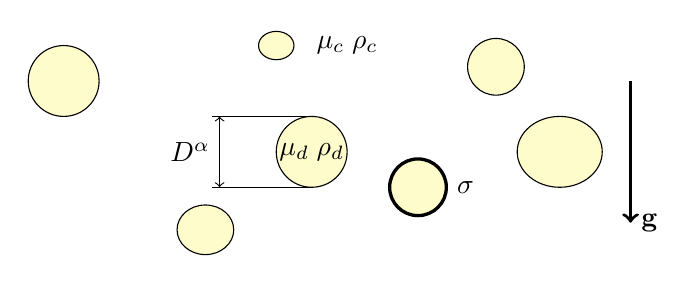
\begin{tikzpicture}[scale = 0.9]
        \draw[fill=yellow!20](3,3) node{$\mu_c\;\rho_c$};
        \foreach \x/\y/\ra/\r in {2/3/0.2/0.25,
        5.1/2.7/0.4/0.4,
        1/0.4/0.35/0.4,
        4/1/0.4/0.4,
        6/1.5/0.5/0.6,
        -1/2.5/0.5/0.5}{
            \draw[fill=yellow!20](\x,\y) ellipse(\r cm and \ra cm);
        }
        \draw[fill=yellow!20](2.5,1.5) circle(0.5)node{$\mu_d\;\rho_d$};
        \draw[thin,-](1.1,2)--++(1.4,0);
        \draw[thin,-](1.1,1)--++(1.4,0);
        \draw[very thick,black!80!black](4,1) ellipse (0.4cm and 0.4cm);
        \draw[very thick,black!80!black](4,1)++(0.4,0)node[right]{$\sigma$};
        \draw[thin,<->](1.2,1)--++(0,1)node[midway,left]{$D^\alpha$};
        \draw[very thick,->](7,2.5)--++(0,-2)node[right]{$\textbf{g}$};
    \end{tikzpicture}
    \caption{Scheme of droplets immersed into a continuous fluid phase.}
    \label{fig:scheme}
\end{figure}

There is a total of $9$ independent physical parameters to this problem (if we consider only the mean of the sizes $D$), they are all constituted by 3 fundamental units, a length, a mass and the time.
Therefore, according to Buckingham $\Pi$ theorem we can define a minimum of $9-3 = 6$ dimensionless numbers to describe the problem. 
Several options are available the selection is somewhat arbitrary, so we choose the following set of dimensionless numbers. 
The $4^{th}$ first parameters are linked to the physical properties of the emulsion, namely, 
\begin{align*}
    & Ga^2 =\frac{\rho_c(\rho_c - \rho_d) g D^3}{\mu^2_c}& 
    & Bo =\frac{(\rho_c - \rho_d) g D^2}{\sigma}&
    & \mu_r = \frac{\mu_c}{\mu_d}& 
    & \rho_r = \frac{\rho_c}{\rho_d}&
\end{align*}
And the two remaining parameters are related to the topology of the flow, 
\begin{align*}
    \phi = \frac{V_d}{V_c} & &
    N_b = \frac{6V_d}{\pi D^3}
\end{align*}
with $N_b$ is the number of droplets in the volume considered and $\phi$ the volume fraction of the dispersed phase.
The \textit{Galileo number} or \textit{Archimedes number}, is the ratio of the buoyancy forces over the viscosity forces, noted $Ga$.
Note that the \textit{Reynolds number}, defined by, $Re = \rho_c L U/\mu$, where $U$ is the characteristic velocity, is equivalent to the \textit{Galileo number} if we take $U = \sqrt{gL(\rho_c-\rho_d)/\rho_c}$ as the velocity scale.
$Bo$ is the \textit{Bond} or \textit{E\"otv\"os number}, it is the ratio between the buoyancy forces and surface tension forces. 
Notice that $We = Bo/Ga^2$, with $We$ the \textit{Weber number} compares the viscous forces with capillarity forces.
Thus, $We$ describe the deformation of the droplets, as an example, above a critical value of the \textit{Weber number} a droplet will break due to hydrodynamical forces \citet{deike2022direct}. 
Lastly, $\mu_r$ and $\rho_r$ are respectively the density and viscosity ratios. 

To give a brief idea about the range of interest of those numbers in the industrial context, we take the example of an oil/water emulsion.
In the real processes the diameter of the droplets lies in the range $D = [10 \mu \text{m}, 1 \text{mm}]$.
The density and viscosity of water are approximately $\rho_c = 1000 \text{kg/m}^3$ and $\mu_c = 10^{-3}$.
The density and viscosity of oil are close to $\rho_d = 900 \text{kg/m}^3$ and $\mu_d = 10^{-2}$.
We consider the gravity acceleration on earth, thus it is $g= 9.81 \text{kg.m.s}^{-2}$.
The surface tension of the system oil/water is known to be approximately $\sigma = 50 \text{mJ/m}^2$ \citep{de2015gouttes}. 
We display the values of dimensionless parameters computed with those physical parameters in \ref{tab:parameters}.
\begin{table}[h!]
    \centering
    \caption{Dimensionless parameters for a water/oil emulsion.}
    \begin{tabular}{|c||c|c|c|c|c|}
        \hline&$Ga$&$Bo$&$\phi$&$\mu_r$&$\rho_r$\\ \hline
        \hline Oil/Water&$[0.03,30]$&$[10^{-6};10^{-2}]$&$[0,0.15]$&$0.1$&$1.111$\\ \hline
    \end{tabular}
    \label{tab:parameters}
\end{table}
We can notice that the \textit{Galileo number} is rather low therefore can already state that it will be necessary to investigate the stokes flow limit. 
Likewise, The \textit{Bond number} is very low, meaning that the droplets are nearly spherical.
Consequently, in the following models and numerical simulations we must consider some cases with spherical particles. 
The viscosity and density ratio as well as the volume fraction do not permit any additional assumption on the flow. 

\section{Current state of dispersed two-phase flow  modeling}

Up to now a lot of investigations have been made on the modeling of bubbly flows.
Indeed, bubbly flows are of large interest since they appear in plenty applications (especially the nuclear industry).
Consequently, researchers have been trying to find closure terms on the specific case of bubbly flows. 
For these reason, most of the studies cited below investigate bubble hydrodynamics (and not droplets). 
Also, in the perspective of modeling the reactor scale authors have developed software carrying out Euler-Euler simulations. 
The most famous ones are NEPTUNE-CFD belonging to EDF, and OpenFoam with its collection of multiphase solvers. 
Again, most of the authors carried the computation of the averaged equations of bubbly flows and not emulsion.
Even though in this thesis we solely focus on the closure terms calculation, it is of interest to say a few words on the modeling of the upper scale.
i.e. the industrial scale, where we solve the averaged equations derived in \ref{chap:avg}. 

\subsection{Macro scale modeling with CFD-PBM}
Here is a brief review of the authors who attempted to carry out CFD-PBE simulation.
\citet{wang1995simultaneous} study numerically the PBM equations for buoyancy-driven setting of spherical drops suspension.
They consider a one-dimensional PBE for the axis along the column. 
And solve for the continuous size distribution function $f$.
The source terms $B(n)$ are modeled using the theoretical formulas depicted in the previous chapter, and the probability of coalescence is assumed to be 1 since there is no bouncing in the absence of inertia (therefore a contact results always in coalescence). 
In this context, they could solve the equations, and they show how the coalescence influences the phase separation inside a vessel.
In \cite{KAMP20011363} they solve numerically the averaged PEB considering one dimensional and spherical bubbly flow.
They solve the first and second-order equations of the PBE.
They also considered the velocity of the bubbles as independent of the bubble size. 
The coalescence kernel is derived for unequal bubble size interaction in turbulent flows. 
The results are validated with experimental data on pipe flows under microgravity conditions. 
They could show that the coalescence rate diminishes between the inlet and outlet due to the decrease in the rate of collision because the velocities of collision are higher. 

Next,  \citet{morel2010comparison} performed simulations of Euler-Euler models coupled with PBE for bubbly flow columns. 
They considered 4 different situations with different hypotheses, namely, the single-size approach, the moment approach based on the log-normal distribution, the moment approach based on the quadratic law, and the multi-fields approach.
The latter method is also called the class method mentioned in the previous chapter (it consists of solving the N equations for the mass and momentum of the N class of particles).
They conclude that from the first to the last method the accuracy increased together with the numerical cost.
Apart from the last method which is completely different from the others and turns out to over-predict coalescence. 
Now, in \citet{gemello2018modelling} a full CFD-PBM is modeled for bubbly column on the code \texttt{OpenFoam}. 
The CFD part is modeled with the averaged Navier Stokes equation.
They use classic turbulence model (i.e. $k-\varepsilon$ model, RNG $k-\varepsilon$ and $k-\omega$ model) to account for the velocity fluctuation term, $\left<\bm{u}'\bm{u}'\right>^f$. 
They conclude that $k-\omega$ was the most practical model in terms of accuracy and stability.
\citet{alam2022cfd} conducted CFD-PBM and experimental study on a nano-bubble generator. 
They also compared different turbulence models and found out that the $k-\omega$ model predicted a better prediction for high flow rates.
Note that this modeling of the pseudo-turbulent tensor is not physical as pseudo-turbulence is different from classic turbulence.
A slightly different work is done by \citet{salehi2017population}, they coupled Large Eddy simulation to PDF-PBM to predict the distribution shape and size of droplets in atomization turbulent flows. 
The dispersed phase is here modeled with a Lagrangian approach, the drag force term uses the mean velocity difference between the averaged continuous phase and the dispersed phase.
The additional feature of this work is that they take into account the size and the shape as variable in the droplet distribution.
The strategy of stokes binding is used here, this method consists in representing one notional particle for a particle size.

Though, all the processes modeled by these authors involve poly dispersed two-phase flow, none or few of them, are considered accurate closure for the velocity fluctuation (they often consider turbulence-like models) and the other first order moments closures terms are neglected. 
The reason is that no accurate closure terms exist yet in the literature. 
Only the drag forces seem to be predicted from robust semi-empirical correlations, for bubbly flow at least.

\subsection{DNS modeling of suspended particles or droplets}

Now, let's focus on the numerical studies providing empirical expression for the closure terms. 
Numerous authors worked on the topic, and most of them are already mentioned in the previous chapter regarding their theoretical work. 
Note that all the following articles are rather recent since DNS of bubbly flow is quite expensive and has been achievable for only a few years. 
\citet{esmaeeli2005direct} carried out  DNS of representative periodic volume of bubbly flow. 
They measure the rising velocity, velocity fluctuation as well as the relative orientation of the pair of bubbles.
Furthermore, they could predict the averaged rising velocity reasonably well, as it is the simplest quantity to predict among all the closure terms.
Indeed, the rising velocity is the quantity that converges faster than the other thus less sample is needed to predict it.
At the time they were limited by computer performances, thus, the maximum Reynolds number archived is $Re  = 77$, indeed more grid points are needed for higher $Re$. 
They simulated deformable and non-deformable bubbles.
The main difference is that the spherical bubbles form \textit{raft} where the arrangement of the deformable bubbles is pretty random. 
They also found a Gaussian distribution for the velocity fluctuation.
In a more recent work \citet{willen2019resolved} simulated equal spheres in an upward flow.
They also compute the velocity and velocity fluctuation and show that the suspension was anisotropic in the direction of the gravity force.
Besides, they also measured the structure of the flow and recovered the column arrangement and horizontal arrangement, to analyze the structure they used tetrads which allowed them to see the evolution of the relative positions.
\citet{du2022analysis} perform DNS calculation of mono disperse bubbly flow and focus on the calculation of pseudo turbulent tensor. 
They separate the pseudo turbulence tensor into two contributions.
The wake-induced turbulence and the potential flow and averaged wake fluctuation.
The former is the main focus of the study and a model is proposed.
% All these studies used DNS and analyzed the closure by computing it directly.
% However, other authors considered wave analysis to get the closure terms. 
% We won't go into details, but it is possible to compute several closures by the analysis of the wave speed.
% For more information we point the reader to the following articles,  \cite{duru2002constitutive}, \citet{willen2017continuity} and\citet{derksen2007direct}.
On another hands \citet{wang2021numerical} performed DNS of a random array of fixed spherical particle.
About 3000 spheres were modeled to get a representative sample. 
They computed the PFP stress based on the nearest particle statistic.
They show that this particle stress can predict the skewing effect along the flow direction and repealing effects on the normal directions of the particular phase. 
This is the only study reporting the calculation of the PFP stress therefore a need is clearly needed on this matter.
\citet{manga1995collective} studied experimentally as well as numerically, with boundary integral methods, the rate of coalescence of interacting pairs of drops.
They investigated the influence of deformation on the rate of coalescence and concluded that the greater the drops or bubble deform (for high $Bo$ and  $Ga$) the higher the probability of coalesce will be (might go up to one order of magnitude above than for non-deformable drops).
It also results in a wider distribution of the particle size.
\citet{innocenti2020direct} simulated 3D column of rising bubbles and evaluated velocity fluctuation and energy dissipation for turbulence. 
\citet{hidman2023assessing} simulated tri-periodic simulation of rising mono-dispersed bubbly-flows. 
Interestingly their simulations'  setup is close to what we wish to accomplish. 


From all the studies presented above it seems that getting the closure terms through DNS seems well achievable.
The most suited setup in our case seems to be the simulation of random arrays of bubbles, similarly to \citet{hidman2023assessing}.
Indeed, they could measure the velocity fluctuations properly and other closures like the drag forces (through the averaged velocity) and also terms related to turbulence modeling and transport of passive scalar. 
Additionally, to avoid the modeling of a large domain they make use of periodic boundary conditions, which is what we will do.
This way we will be able to provide closure terms for buoyant driven emulsion.
In the next section, we present the methodology to carry out massive DNS of a tri-periodic random array of rising drops.



% \section{Basilisk a suited software to perform massive DNS calculations.}

In view of the previous research (especially the study of \citet{innocenti2020direct}) and the good results obtained in \citet{Naanouh2021numerical}, we thought that the partial differential equation solver, Basilisk (from \url{basilisk.fr}), was the most suited code to carry out tri-periodic simulation of buoyant droplets. 
Originally this code is based on the older code,  \texttt{Gerris}, and was developed primarily by Francesco De Vita, Jose-Maria Fullana, Geoffroy Kirstet-ter, Pierre-Yves Langrée, Emily Lane, Jose Lopez-Herrerra, John MacFarlane, Stéphane Popinet, Clément Robert, and Antoon van Hooft .
Both codes are open source, that is why since then the community contributed to the development of Basilisk and numerous authors published their contribution to the code in scientific reviews.
The open source aspect of Basilisk is somewhat essential for us since it enable us the to develop any desired features.
Besides, a lot of benchmarks demonstrated the good performances and the broad abilities of Basilisk.
All the algorithms are developed in C, if well done this language has the great advantage of optimizing the memory management, resulting in a better computation efficiency. 
Moreover, a lot of physical solvers are already implemented in the code, from wave modeling \citet{mostert2022high} to the simulation of suspended solid particles in a fluid using immersed boundary method \citet{shui2015direct}.
A last feature that has been recently implemented in Basilisk is the multilayer solvers \citep{popinet2020vertically} which will be of great interest in the modeling of film drainage problems. 
We refer the reader to this link \url{http://basilisk.fr/src/README} to see the whole range of possibilities offered by Basilisk.
Nevertheless, the most interesting feature for our use is the capability of modeling two phase flow in Basilisk. 
Indeed, the Volume-Of-Fluid (VOF) method implemented in Basilisk have shown great performance and accuracy, (see \citet{popinet2009accurate}\citet{popinet2018numerical}). 
This point will be developed in a following section since it is of major importance. 
Another practical aspect of Basilisk is that the meshing is included in the workflow of the simulation. 
This enables the possibility of switching between 2D cases and 3D cases automatically, indeed the \textit{dimension} parameter need to be switch from 2 to 3 the rest is automatic. 
In our case it is of a great use since we will start by carrying out 2D simulations and after validation we will switch to 3D mesh.
Speaking of the mesh, Basilisk provide several mesh types that considerably improve the efficiency of the calculation.
The first one is the classic Cartesian mesh, it is fully orthogonal, this is the most for mono-scale problem.
Another interesting grid is the adaptive mesh, as indicate by its name this mesh refines the area where high velocity gradients is observed.
\citet{innocenti2020direct} model a large quantity of bubbles in a container, this was only possible thanks to the adaptive mesh solver, otherwise it would have been too expansive.
The simulation of wave crashes by, \citet{mostert2022high} was made possible also thanks to the adaptive mesh refinement.
Numerous other examples testify of the usefulness of the adaptive mesh refinement solver.   
Then the last meshing technics is a subcase of the adaptive mesh, it is the \texttt{multigrid} mesh, presented in \citet{popinet2003gerris} for the incompressible Euler equations, and more recently in \citet{popinet2015quadtree} for the fully-nonlinear Boussinesq wave equations. 
This meshing technics consist in working with different levels of refined grids simultaneously.
More details will be given about the meshes in this section. 
Finally, the last point on which we would like to emphasize is that Basilisk is a self independent software (i;e. Only the source code of basilisk is needed to compile it) and simulations are launch via C files. 
Which makes it practical for the execution on any machines (cluster or not). 
In the next sections we present the specificity of the VOF methods, needs we speak more specifically about our numerical setup to model rising suspension of droplets. 



\subsection{The Volume Of Fluid Method}

The VOF method is used to model two-phase (or more) flows. 
The governing equations, solved by our solver in the present case, are the one-fluid formulation equation of momentum and mass, presented in \ref{chap:avg}. 
We recall their form here, 
\begin{equation}
    \pddt (\rho \textbf{u})
    = \nablabh \cdot (\textbf{T} -\rho  \textbf{u} \textbf{u})
    + \textbf{b}
    + \textbf{f}_I\delta_I
    \;\;\;\text{and}\;\;\;
    \pddt \rho
    = 
    - \nablabh\cdot(\rho\textbf{u}_k). 
\end{equation}
Note that the material properties (i.e. $\rho$ and $\mu$) takes the value of the phase in presence. 
As seen in \ref{chap:avg}, in two phases flows we define a phase indicator function $\chi$, which is a marker to identify the phases in presence.
When, $\chi = 1$, we are located in the dispersed phase, when $\chi = 0$ in the fluid phase for example, therefore $\chi$ correspond to a Heaviside function. 
However, the Heaviside function is not continuous and derivable everywhere. 
This latter point makes the use of $\chi$ impossible in numerical method.
Therefore, in CFD code, we use an approximation of the Heaviside function, namely the color function $C$. 
Since we want to follow the phases with time,  we need to add the equation of transport of $C$ to complete the system, namely,
\begin{equation}
    \frac{\partial C}{\partial t} + \textbf{u}\cdot\bm{\nabla} C = 0.
    \label{eq:cfunc} 
\end{equation}
At this point several methods are available to define $C$ and to discretize these equations. 

Regardless of the definition of $C$ it is important to say a few words on the discretization of the Navier-Sokes equations which is independent of this choice. 
Basilisk uses the finite volume based method to discretize the governing partial differential equations.
A full review of the finite volume method is made in the book \citet{ferziger2002computational}.
The finite volume method consists in discretizing the whole domain of fluid by finite volume called cells. 
This discretized domain is what we call a mesh. 
In Basilisk we use only orthogonal meshes. 
Which means that the cells of the domain are only squares or cubes.
Nevertheless, as mentioned in introduction there are several specificities among these orthogonal grids.   
\begin{figure}[h!]
    \centering
    \begin{tikzpicture}
        \node (a) at (-0.25\textwidth,0){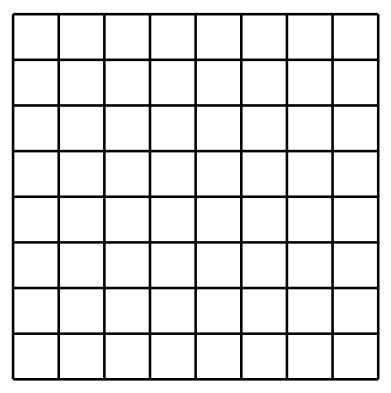
\includegraphics[height = 0.2575\textwidth]{image/pic/Uniforme.png}};
        \node (b) at (0,0){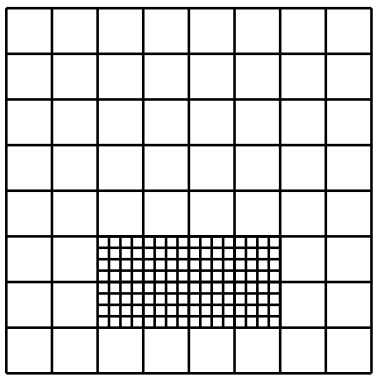
\includegraphics[height = 0.25\textwidth]{image/pic/non-uniform.png}};
        \node (c) at (0.25\textwidth,0){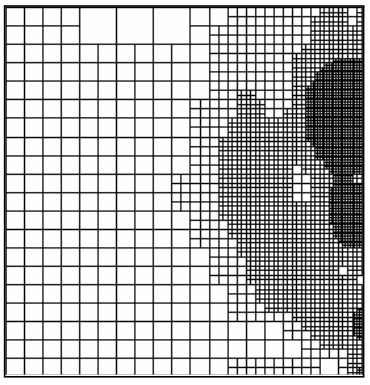
\includegraphics[height = 0.25\textwidth]{image/pic/adaptativemesh.png}};
        \node (leg) at (a.south){(a)}; 
        \node (leg) at (b.south){(b)}; 
        \node (leg) at (c.south){(c)}; 
    \end{tikzpicture}
    \caption{Different type of orthogonal meshes. (a) uniform mesh, (b) Non-uniform mesh, (c) Adaptive \textit{Quad/Octree} mesh. Reprinted from \citet{mani2021numerical}. }
    \label{fig:meshes}
\end{figure}
The first one is the classic uniform grid depicted \ref{fig:meshes} where all the cells have the same size.
The second one is the non-uniform grid. 
It is useful when the user need to refine a specific area of the mesh, due to high local gradient of the velocity for example.
Then, the last one, is the Adaptive \textit{Quad/Octree} Grids, on which we are to give a bit more details.
It consists in subdividing the cells into $2^2$ cells in two dimension, or in $2^3$ cells in 3 dimension. 
Each cell that have the same size form a group.
All the groups are referred by their respective \textit{levels}. 
The group of level 0 is the one with the larger cells size, actually at this there is only one cell of the size of the domain. 
Then as we look at higher levels the size of the cells decrease. 
Besides, Basilisk offer the possibility of the \textit{Adaptive} option. 
Which means that the cells are subdividing or merging themselves automatically all along the simulation time. 
At the frontier between two levels there is what we called the \textit{resolution boundary}. 
Those boundaries, are somewhat problematic since the cells on each side are not of the same size.
Therefore, the basic operation of the finite volume method are not trivial anymore. 
To avoid this issue Basilisk use \textit{halo cells}.
One \textit{halo cell} is the representation of the cell of the lower level that gather the mean value of the four smaller cells.
The former cell is of the same size of the cell at the other side of the \textit{resolution boundary}, that is why the system is consistent. 
In Basilisk the cells from which the \textit{halo cells} are build are called the children cells, therefore the lower level cells are the parent cells. 
This principle is used for the adaptive mesh, nevertheless, the \textit{Quad/Octree} grid has one subclass, the \textit{multigrid} mesh. 
This meshing technics is no more than a uniform mesh where we make use of the \textit{halo cells}, and parent/children principle. 
Even though there is no \textit{resolution boundary}, this technics allows the user to loop through different levels and through each branch of the mesh. 
This feature is of a great interest to carry out fast operations on vector or scalar fields. 
We refer to the publication of \citet{popinet2015quadtree} for a more detailed explanation.  
Once the mesh is set one need to discretize the governing equations in space and time (see \citet[chapter 3]{tryggvason2011direct}). 

Five main option exist to define the color function $C$ :
the volume of fluid method,
the front taking method,
the level-set method,
the phase-field method
and the CIP method.
As the title of this section is the \textit{volume of fluid method} one could guess which one we use. 
For more details on the other methods we refer the reader to \cite[Chapter 4]{tryggvason2011direct}. 
With the Volume-of-fluid method the color function is now defined by a \textit{VOF tracer}, $f_i$, where $k$ stand for the indices referring to the phase. 
For $N$ VOF tracer $f_k$ is defined for $0\leq k\leq N$.
From $k=0$ for the continuous phase to $k=1$ to $N$ for the dispersed phases (in case we have $N$ dispersed phases). 
In practice the function $f_c$ is not computed since we have the relation, $f_c = 1- \sum_{k=1}^N f_k$. 
The value of the $f_k$ is comprised between $0$ and $1$.
$f_k = 0$ meaning that the concentration of phase $k$ is null, $f_k = 1$ meaning that $100\%$ of the volume is occupied by the phase $k$. 
Note that in every cell the value of $f_k$ is either $0$ or $1$, except in the cells including an interface where the value is the percentage of the phases in presence.
\begin{equation}
    f_k = \left\{\begin{tabular}{cc}
        $1$  &if $\textbf{y}\in V_k$\\
        $0$  &if $\textbf{y}\in V_c$\\
        $0$ to $1$  &if $\textbf{y}\in V_c \cap V_k$\\
    \end{tabular}
    \right.,
\end{equation}
where $V_k$ is the volume occupied by the phase $k$.
The overall condition is that $\sum_k^N f_k \leq 1$.
Next, if we note $\rho_k$ and $\mu_k$ the material property of phase $k$ we can finally compute in each cell the value of the material properties,
\begin{equation*}
    \rho 
    = \sum_k^N \rho_k f_k 
    + (1-\sum_k^Nf_k)\rho_c 
    \;\;\;\text{and}\;\;\;
    \mu 
    = \sum_k^N\mu_k f_k 
    + (1-\sum_k^Nf_k)\mu_c.
\end{equation*} 
In the neighboring cells of the interfaces the calculation of $\rho$ and $\mu$ are slightly different \citep{tryggvason2011direct}. 
Then, once the material properties are calculated, the Navier-Stokes equations solved and the VOF tracers advected, the last step is to reconstruct the interfaces from the $f_k$.
To do so, several methods, more or less accurate, are available  to us.
\ref{fig:VOF} depicts the different reconstruction method, namely, the Simple Line Interface Calculation or SLIC method, the Hirt and Nichols reconstruction method and the Piecewise Linear Interface Calculation or PLIC method. 
As we can clearly see on the scheme the methods goes from coarse (with SLIC) definition of the interface to a more accurate reconstruction (with PLIC).
\begin{figure}
    \centering
    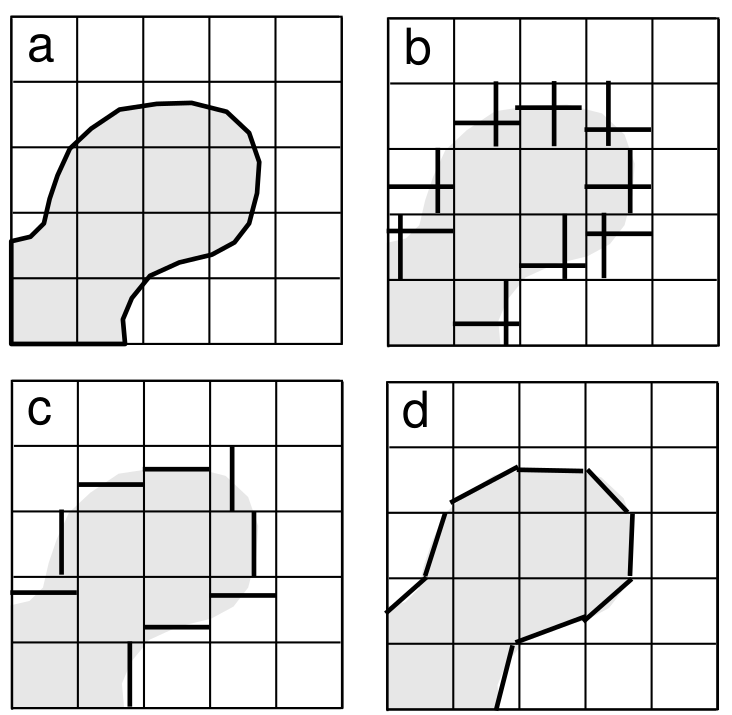
\includegraphics[width = 0.4\textwidth]{image/pic/VOF.png}
    \caption{VOF reconstruction of the solution for advection in two dimensions. 
    (a) The original interface. 
    (b) The original SLIC reconstruction. 
    (c) The Hirt and Nichols reconstruction. 
    (d) PLIC reconstruction. 
    Reprinted from \citet{tryggvason2011direct}.}
    \label{fig:VOF}
\end{figure}
In Basilisk we use PLIC method using height functions (see \citet[Chapter 5]{tryggvason2011direct}). 
Here is a quick summary of how height functions work.
Each segment is parametrized by its normal $\textbf{n}$ and the intercept of a line, $\alpha$. 
Then, in the local reference frame of coordinate $\textbf{z}$, it is possible to define the interface by,
\begin{equation}
    \textbf{n}\cdot\textbf{z} 
    = \alpha,
\end{equation}
where $\alpha$ is computed with the local volume fraction of the phase and the unit normal. 
The overall error is of second order. 
Nevertheless, it must be said that even though the PLIC method is accurate, it still has some draw back sheared with the two other methods. 
Indeed, if we consider 2 tracers the interface is reconstructed considering the tracer $f_c$ and the tracer $f_1$.
Which is equivalent to consider two phases, up to now everything is normal. 
But, consider two interfaces getting closer, then at some point the interfaces will merge together discarding the physical aspect.
Indeed, since we compute height functions from the local volume fraction, if two drops with the same tracer met, then the interfaces are reconstructed regardless of the physical geometry. 
Another problem is that VOF tracers are advected separately so interpenetration of different VOF tracers can happen (this issue will be developed in the next section). 
These two facts mandate the use of a relatively fine mesh so that the film between the droplets is partially resolved.

Once the interface is reconstructed, we can tackle the most challenging problem of VOF simulations.
Which is the modeling of the surface tension forces, i.e. the source term, $\textbf{f}_I\delta_I$, in the one-fluid formulation equations.
Obviously we will not detail the solutions here, to get an overall vision of the problem we refer the reader to \citet{popinet2018numerical} or  \citet[Chapter 7]{tryggvason2011direct}.
However, we can cite the two most basic method.
The first one is the \textit{Continuous surface force method}, in consist in discretizing the expression of the surface force source term. 
Note that the expression of $\delta_S$ make use of the color function, it is in fact equal to the gradient of the color function. 
The approximation of the surface force source term is then,
\begin{equation}
    \sigma \kappa  \textbf{n} \delta_I 
    = \sigma \kappa \nabla f_i,
\end{equation}
where the curvature $\kappa$ is estimated through height function \citep{popinet2018numerical}. 
The other method is the \textit{Continuous surface stress method} which is equivalent, but instead of discretizing the force term, we discretize the divergence of a stress.
It reads, 
\begin{equation}
    \textbf{f}_I \delta_I = \nabla \cdot \left[\sigma (\textbf{I}-\textbf{nn})\delta_I\right],
\end{equation}
\tb{Find were does that came from}
which is valid even with non-constant $\sigma$. 
In Basilisk, we make use of the former method. 

The overall difficulty encountered in the two-phase flows simulations is to manage the singularities at the interfaces.
Indeed, it is a common problem in mathematic when the function is not derivable everywhere.
Hence, from a numerical point of view it is no less of a problem. 
In the conclusion of this chapter we will review some issues arising in  the simulation of emulsion because of this point. 

\subsection{Numerical coalescence}

As briefly mentioned in the preceding section, numerical coalescence can occur during a simulation if two interfaces are one cell mesh apart (assuming there is a solely VOF tracer). 
However, in \ref{chap:avg} we showed that the coalescence of two droplets is a multiscale phenomenon. 
At first, it involves hydrodynamical and lubrication forces.
Once the interfaces are close enough Van deer Waals forces are responsible for the coalescence.
The former forces are well modeled when using a fine enough mesh. 
Indeed, we solve the Navier-Stokes equation together with the transport of the color function, which is the basis of the calculation of the lubrication forces \citep{guazzelli2011}. 
However, the latter contribution involve microscale interaction which are not included in this model.
Even though, it is possible to include Van der Waals forces in Basilisk, it would be too expensive to compute the film drainage problem for several droplets at the same time.
To avoid this problem \citet{thomas2010multiscale} modeled the film drainage by allowing coalescence when the contact time of the droplet is greater than the critical time of contact (computed theoretically).  
However, the closure for the contact time is not well define for our parameters yet.
Moreover, before allowing coalescence after a critical time, we need to prevent it anyway. 
Hence, in any cases we need to prevent coalescence event to happen since DNS of the film drainage is too expansive numerically. 
Besides, to create accurate closures terms seen in \ref{chap:avg}, we need to identify accurately the topology of a given situation.
This way we will be able to give the value of a closure term in terms of the exact number and size of the droplets for example. 
This implies that we must keep a constant number of droplets all along the simulation.

Before avoiding coalescence to happen it is important to identify why it does happen. 
The reason why numerical coalescence occurs is that only one VOF tracer is used. 
Indeed, let's take two drops approaching each other. 
The VOF tracer is advected along the velocity fields. 
We recall that in the interfacial area the VOF tracer has a transitional value between $1$ and $0$. 
Therefore, when the drops eventually get close enough the VOF tracer at the interface of the drops meet each other in the same cells. 
Since the same VOF tracer is used for the two droplet, it results in the addition of the values of the VOF tracer at the interfaces since they gather in the same cells. 
Then, as the VOF tracer merge it is impossible to reconstruct the interface of the respective droplets. 

Using different VOF tracer would prevent the drops to coalesce 
Indeed, during advection the VOF tracer will not sum with the neighboring ones thus the reconstruction of the interface will be possible. 
However, in the literature, we see that we need about hundreds of particles to be able to get a representative volume. 
And since we need to advect each VOF tracers independently, it would be too expensive to have one VOF tracer per drops.    
Luckily, we only need that the adjacent droplets at a given time $t$ have different VOF tracer. 
In 2D the famous \textit{four color map theorems} stipulate that we only need 4 color to color adjacent country with a different color (this is a topological proof).
For our concern, it does mean that we will need no more than four VOF tracer in order for the adjacent droplets to have different VOF tracer. 
In 3D this theorem is not valid anymore. 
Moreover, the droplets move within time thus their neighboring particles changes, and they might need a different VOF tracer.

To tackle this issue \citet{mani2021numerical}, developed an algorithm on Basilisk to carry out the previous task automatically. 
Even though, this algorithm is based on empirical observation and not topological arguments it prevents from using too much VOF tracer. 
The workflow is as follows.
In a first step we identify the VOF tracer having droplets that are close to each other. 
Then for each of these VOF tracers, we identify the pairs of droplets. 
Then we check which of the droplets among one pair have the least neighbors. 
Finally, we switch the VOF tracer of the former droplet to a new tracer that is not in the vicinity of the droplet. 
If no VOF tracer is available then we create a new one. 
In the practical case we indeed notice that 2D simulations do not use more than 4 VOF tracers. 
Therefore, this is a proof of the efficiency of the algorithm. 
This algorithm considers a droplet close to another one only if they have VOF tracers two cells apart.
Consequently, if the drops relative velocity is greater than that this length time the time step then the algorithm will not work.
Nevertheless, in practice the CFL condition is respected which means that the distance traveled by a fluid particle is never superior to one mesh cell. 
This algorithm is launched every time step by default, nevertheless we could call it every 2 time steps (since three would be a bit reckless). 
\tb{more details on this matter }
\subsection{Simulation of periodic rising droplets}
As concluded in the two previous sections, we are going to make DNS of a random array of droplet rising in a continuous Newtonian fluid with the code Basilisk. 
Therefore, in this section we are going to present the 


In Basilisk the computational domain of the simulation must be a square in 2D or a cube in 3D, as depicted on \ref{fig:numscheme}. 
Depending on the desired number of bubbles $N_b$ we divide the domain of size $\mathcal{L}$ in $N$ smaller squares of length $\Delta$.
In each smaller squares we initialize the VOF tracers $f_i$ as a spherical, in 3D, or circular, in 2D, shaped area representing the droplets.
Each droplet of diameter $L$ is centered inside their $\Delta\times \Delta$ square.
Besides, we add a random shift vector for each droplet position so that all the simulations with the same parameters are unique. 
The shift must be limited in order to avoid that the drops touch each other at the initialization time (in which case they would immediately merge).   
Also, another method consist of initializing all droplets randomly, making sure that they are initially far enough so that they do not touch each other at the first step of the simulation.
The latter technics was used in the simulation performed in \ref{chap:mono-disperse} since it has shown faster convergence. 
Indeed, as we initialize with a random state, the suspension takes a shorter amount of time to reach it statistically random steady state. 
\begin{figure}[h!]
    \centering
    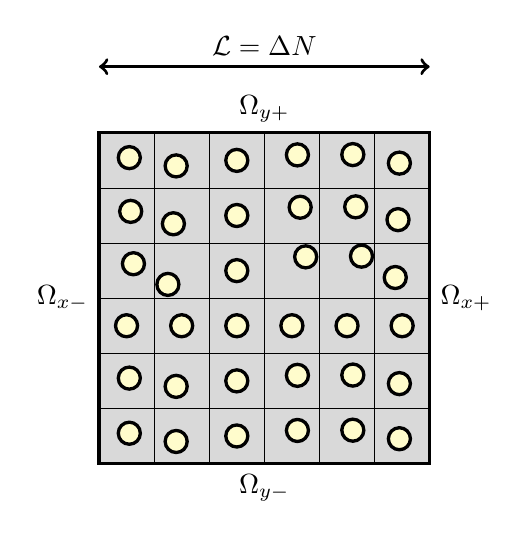
\begin{tikzpicture}[very thick,scale = 0.7]
        \draw[fill=gray!30](0,0) rectangle(6,6);
        \foreach \x/\dx in {0.5/0.1,1.5/-0.2,2.5/0,3.5/0.2,4.5/0.21,5.5/-0.1}{
            \draw[very thin](\x+0.5,0)--(\x+0.5,6);
            \draw[very thin](0,\x+0.5)--(6,\x+0.5);
            \foreach \y/\dy in {0.5/0.1,1.5/+0.1,2.5/0,3.5/0.25,4.5/0.15,5.5/0.1}{
                \draw[fill=yellow!20](\x+\dx*\dy*5,\y+\dy*\dx*5) ellipse(0.2 cm and 0.2 cm);
            }
        }
        \draw[<->](0,7.2)--(6,7.2)node[midway, above]{$\mathcal{L} = \Delta N$};
        \draw(3,6)node[above]{$\Omega_{y+}$};
        \draw(3,0)node[below]{$\Omega_{y-}$};
        \draw(6,3)node[right]{$\Omega_{x+}$};
        \draw(0,3)node[left]{$\Omega_{x-}$};
    \end{tikzpicture}
    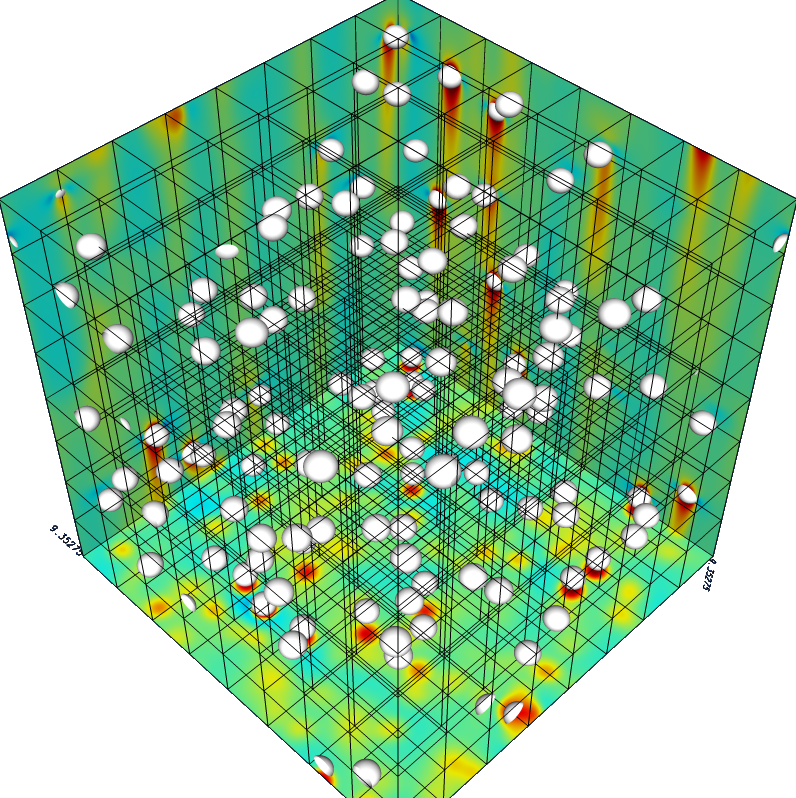
\includegraphics[width=0.45\textwidth]{image/3D/PHI01.png}
    \caption{(left) Scheme of the initialization of an array of droplets immersed in a 2D periodic domain.
    (right) Picture of a 3D simulation with $\phi = 0.1$, $N = 5$ the color represent the velocity field.}
    \label{fig:numscheme}
\end{figure}

The dimensionless parameters of this study have been already discussed in \ref{chap:avg}.
Nevertheless, additional dimensionless parameters must be introduced since numerical parameters that weren't on the theoretical problem appear. 
Only six parameters are needed among the existing dimensionless parameters. 
However, the numerical simulations involve an others length parameters among the ones already mentioned in \ref{sec:introavg}, namely the length of a cell in the mesh.
Therefore, we need to define a new dimensionless parameter, namely, the number of cells per diameter refer by $\delta$. 
From those parameters it is possible to recover the physical parameters needed by the simulation. 
But before we fix the following parameters, $\rho_d = L = g = 1$ for convenience.
Then it yields the following relations to recover the remaining parameters,
\begin{align*}
    &\rho_c = \rho_d\rho_r ,&
    &\mu_d  =\frac{\rho_d \sqrt{|1-\rho_r| \rho_r g \bar{L}^3}}{\mu_r Ga},&
    &\mu_c  = \mu_d\mu_r,&
    &\delta  = D/Nc& \\
    &\sigma = \frac{|1-\rho_r|\rho_d g L^2}{Bo},&
    &\Delta = \sqrt{\frac{\pi D^2}{4\phi}},&
    &\mathcal{L} = \Delta \sqrt{N_b}.&
\end{align*}
From those parameters it is possible to define different time, length and velocity scales. 
It will be useful when we will need to make the results dimensionless. 
The different scales in which we will be interested in are the following.
\begin{align*}
    &U_\mu = \frac{g D^2 \Delta \rho}{\mu_c}&
    &U_\rho = \sqrt{\Delta \rho \frac{Dg}{\rho_d}}&
    &U_\sigma = \sqrt{\Delta \rho \frac{Dg}{\rho_d}}& \\
    &T_\mu = \frac{\mu_c}{g\Delta \rho D}&
    &T_\rho = \sqrt{\frac{\rho_dD}{g\Delta\rho}}&
    &T_\sigma = \sqrt{\frac{\rho_{avg} D^3}{\pi \sigma}}&
\end{align*}
Were $U_\mu$, $U_\rho$ and $U_\sigma$ are respectively the viscous inertial and capillary velocity scales. 
Similarly, $T_\mu$, $T_\rho$ and $T_\sigma$ are the corresponding time scales. 
Here is a quick explanation of the physical meaning of those scales :
When $Ga \ll 1$, in one unit of $T_\mu$ a droplet travel a distance of $D$ relatively to the fluid.  
Similarly, When $Ga \gg 1$ a droplet travel a distance of $D$ in one unit of $T_\rho$. 
Lastly, the Capillary time $T_\sigma$ will be the period of one undulation of the surface droplet. 
Of course this scale provide us with an order of magnitude, they aren't exact. 

In Basilisk the set-up of a simulation (solvers and parameters) is made by including or excluding header files.
All the header files can of course be found in the sources of the code (\url{http://basilisk.fr/src/}).   
In the following, we describe the header files used in this simulation. 
The first one has in fact already been mentioned, it is \href{http://basilisk.fr/src/grid/multigrid.h}{multigrid.h} or  \href{http://basilisk.fr/src/grid/multigrid3D.h}{multigrid3D.h} file for 3D simulations. 
It set up a uniform staggered multigrid mesh. 
Then, we add the file \href{http://basilisk.fr/src/navier-stokes/centered.h}{centered.h} to resolve Navier Stokes equation on this mesh with centered formulation.
The \texttt{two-phase.h} header set up the VOF tracers and interfaces for two immiscible fluid.
It also set add transport equation of the VOF tracers coupled with the Navier Stokes solver.
To account for the tension surface forces mentioned in the previous section we include the \href{http://basilisk.fr/src/tension.h}{tension.h} header file. 
This file takes in account the curvature calculation of the interface and the interfacial forces. 
We then add the \href{http://basilisk.fr/sandbox/fintzin/Rising-Suspension/no-coalescence.h}{no-coalescence.h} header which create several VOF tracers depending on the needs in order to avoid coalescence. 
Finally, the \href{http://basilisk.fr/src/view.h}{view.h} and \href{http://basilisk.fr/src/output.h}{output.h} header are included manage the graphical output.  

As mentioned earlier  the boundaries of the domain are periodic. 
It signifies that the velocity field follow the these conditions,
\begin{align}
    \bm{u}(y_i = 0,t) = \bm{u}(y_i = \mathcal{L},t) \;\;\; &\forall \bm{y} \in \Omega_{y_i-} \;\;\;\text{and}\;\;\; \forall i \in \left\{1,2,3\right\}.\\
    \bm{u}(y_i = \mathcal{L},t) = \bm{u}(y_i = 0,t) \;\;\; & \forall \bm{y} \in \Omega_{y_i+} \;\;\;\text{and}\;\;\; \forall i \in \left\{1,2,3\right\}.
\end{align}
And the pressure fields respect similar conditions, 
\begin{align}
    p(y_i = 0,t) = p(y_i = \mathcal{L},t) \;\;\; &\forall \bm{y} \in \Omega_{y_i-} \;\;\;\text{and}\;\;\; \forall i \in \left\{1,2,3\right\}.\\
    p(y_i = \mathcal{L},t) = p(y_i = 0,t) \;\;\; & \forall \bm{y} \in \Omega_{y_i+} \;\;\;\text{and}\;\;\; \forall i \in \left\{1,2,3\right\}.
\end{align}
The advantage of using periodic domain is that we can run the simulations for an arbitrary long times since the droplets loop inside the domain.
Besides, it lets the flow develop freely, which is more physical for representative volume. 
However, it has some drawback.
The first  one is that the physical phenomenons that have a wavelength larger than the domain won't be represented. 
Therefore, the domain still needs to be large enough to represent the desired phenomenons.
And the other one is that, if we were to model the problem as it is, we would see both phases falling though a Cartesian multigrid mesh. 
Indeed, we apply an acceleration $g$ on the whole domain. 
And since our domain is periodic the velocity field will keep accelerating through the infinite domain.
If we discard the numerical issues this is not a problem.
Indeed, we could still measure the relative velocities and fluctuation over the domain. 
But, the thing is that we can not discard the numerical issues. 
Therefore, we set the simulation in the referential of the fluid phase by applying an acceleration $\bm{a}$ on the whole domain equivalent to a null averaged force.
Namely, 
\begin{equation}
    \textbf{a} = - \left[1-\frac{\left<\rho\right>}{\rho}\right]\textbf{g},
\end{equation}
where we use the volume average operator defined in \ref{chap:avg}.
We can notice that the contribution of the force on the whole numerical domain is null.
Indeed, it yields, 
\begin{equation}
   \int \rho\textbf{a} g(\textbf{x,y}) dV 
    = \textbf{g}\int \rho g(\textbf{x,y}) dV -\textbf{g}\left<\rho\right>\int g(\textbf{x,y}) dV 
    =0,
\end{equation}
where we recognized in the last equation the volume average of the density $\rho$.
Now, the net averaged velocity of the domain will be in null in both direction.
Besides, by applying a constant acceleration through the domain we preserved the relative motion.
However, it turns out that this last fact ins't true in practice. 
Indeed, numerical error accumulation of the momentum at the interfaces occurs due to the inconsistency of the numerical schemes (see \citet{popinet2018numerical}).
Besides, due to the discontinuity at the interfaces solvers can either conserve the momentum or the velocity depending on the numerical schemes used.
In our case we conserve the velocity and not the momentum. 
In Basilisk C we could use the \href{http://basilisk.fr/src/navier-stokes/conserving.h}{conserving.h} solver.
Anyhow, as this problem come from different source it is rather difficult to solve it properly.
As an example in the CFD-DEM code \href{https://hal.archives-ouvertes.fr/hal-02170320}{PeliGRIFF}
they directly force a null velocity fields inside the solver steps. 
As this solution is rather sophisticated we choose for another option. 
Indeed, to solve this problem we add an artificial acceleration on the whole domain at each time step. 
If $U_\epsilon$ is the bulk velocity (which should be theoretically null), then the acceleration to cancel this velocity must be equal to $U_\epsilon/\Delta t$ where $\Delta t$ is the current time step. 
In the next pages we will refer this artificial acceleration as the \textit{momentum correction}. 


% 
\section{Validation of the model}

The numerical parameters introduced in the previous section, i.e. the definition of the mesh $\delta$, and the number of droplet per domain $N$ or $N_b$ (see the definition in the previous section) need to be verified. 
Indeed, in view of carrying a numerous amount of simulations it is important to identify the minimum necessary number of droplets per domain and definition of the mesh.
Clearly, if we keep the parameter $\phi$ fixed a larger number of droplets implies a larger domain, therefore a greater numerical cost.  
Besides, the range of physical parameters needed to obtain representative closure need to be investigated to. 
Therefore, in this section we identify the ranges of numerical and physical parameters in order to obtain an efficient framework. 
The validations are all based on parameter independence arguments, meaning that we keep track of a quantity, and validate our model until the quantity is independent of the parameter. 


\tb{\subsection{Comparison with experimental or numerical simulations}
\subsubsection{Comparaison with o rdered array \citet{loisy2017buoyancy} \citep{innocenti2020direct} }
Include and launch simulations with the model of trygvason for buubles 
}
\subsection{Momentum correction}
But firstly, let's validate our last hypothesis, i.e. the \textit{momentum correction}. 
The procedure is the following, we carried out two similar simulations, one with the \textit{momentum correction} referred as the simulation $C1$, and the other without referred as $C0$.
The aim is to compare the values of the closures terms in both simulations and see if there are any differences between $C1$ and $C0$. 
They both have the following dimensionless parameters : 
$Bo = 1$, $Ga = 75$, $\mu_r  =1$, $\rho_r = 1$, $N = 5$ and $\phi = 0.15$. 
In addition, we select a number of cells per diameter $\delta = 15$ so that we intentionally create numerical error (in order to test at the limit of definition our modeling).
Also, both simulations were carried in 3 dimension. 
Of course, we expect no difference between those cases. 
\begin{figure}[h!]
    \centering
    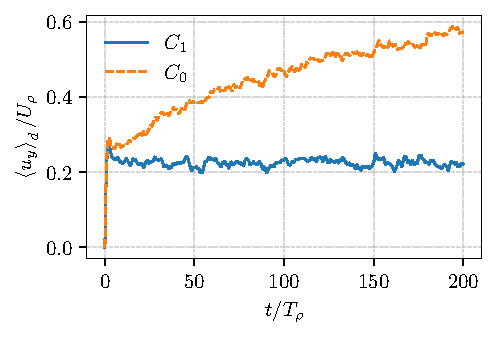
\includegraphics[height= 0.3\textwidth]{image/VALIDATION/C0C1/Ud.pdf}
    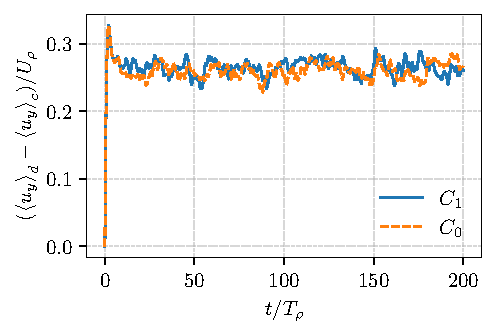
\includegraphics[height= 0.3\textwidth]{image/VALIDATION/C0C1/DeltaU.pdf}
    \caption{(left) Absolute averaged velocity of the dispersed phase along the vertical axis.
            (right) Relative velocity between the dispersed and continuous phases.
            (Dashed lines) simulation $C0$,
            (solid lines) simulation $C1$.  }
    \label{fig:VALIDATION_C0C1_1}
\end{figure}
On \ref{fig:VALIDATION_C0C1_1} we can observe the results of the two cases $C0$ and $C1$.
The (left) picture clearly shows that there is a velocity shift when no correction is applied.
Nevertheless, the two cases exhibit the same interphase velocity (see \ref{fig:VALIDATION_C0C1_1} (right)), which results in a same interphase drag force. 
The phase velocity is a term of first order, therefore it is no sensitive to the numerical parameters (e.g, number of drops per domain, number of cells per diameters).
Therefore, it is interesting to observe on \ref{fig:VALIDATION_C0C1_2}, that the similarities still holds on the first order closure terms. 
\begin{figure}[h!]
    \centering
    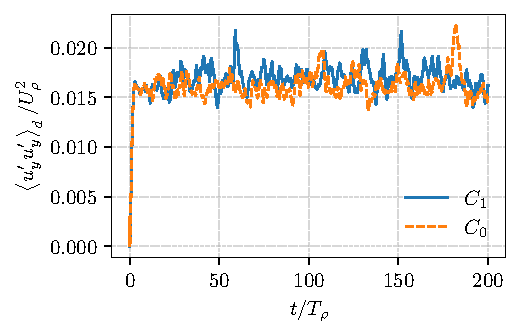
\includegraphics[height= 0.3\textwidth]{image/VALIDATION/C0C1/UpUpf.pdf}
    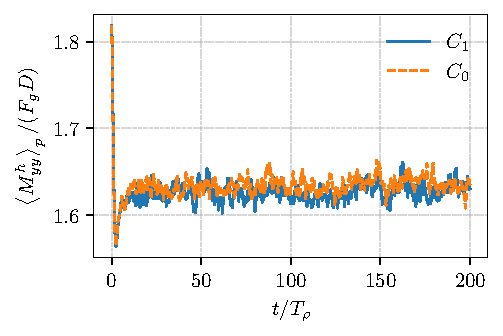
\includegraphics[height= 0.3\textwidth]{image/VALIDATION/C0C1/PA_Mh.pdf}
    \caption{(left) Fluids phase averaged fluctuation tensor.
            (right) Particular average of the first moment tensor, where $F_g$ is the buoyancy force applied on one droplet.
            (Dashed lines) simulation $C0$,
            (solid lines) simulation $C1$.  }
    \label{fig:VALIDATION_C0C1_2}
\end{figure}
Indeed, as we can remark the velocity fluctuations and the first moment are quite the same for both simulations.
It is not presented here, but all quantities remain the same thus the \textit{momentum corrector} isn't influencing any of these closures terms. 

\subsection{Number of particles per domain and definition of the mesh}

Now, let's investigate the required number of droplets per domain, $N_b$, and the minimum definition of cells per diameter of droplets $\delta$.  
\tb{Include bibliography and expectation here \ldots}
For this investigation we kept the physical parameters presented in the same section and made a double parametric analysis over $N$ and $\delta$. 
We carried out simulations for $N = 2, 3, 4, 5, 6, 7$, and for a number of cells $10 <\delta < 40$. 
In Basilisk the mesh definition is defined by a power of two, consequently depending on the size of the domain (which is fixed to keep a $\phi$ constant) the $\delta$ parameter is fixed at a power of 2 close. 
\begin{figure}[h!]
    \centering
    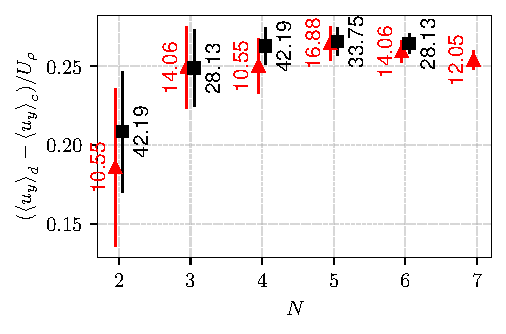
\includegraphics[height= 0.3\textwidth]{image/VALIDATION/N_and_delta/DUd.pdf}
    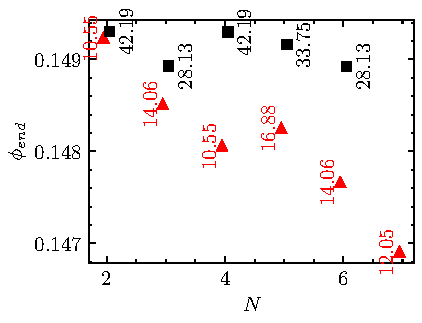
\includegraphics[height= 0.3\textwidth]{image/VALIDATION/N_and_delta/PHI.pdf}
    \caption{(left) Averaged relative velocities for both phases.
            (right) Dispersed phase volume fraction at the end of each simulation.
            The text on the side of the points is $\delta$. }
    \label{fig:VALIDATION_Nd_1}
\end{figure}
\ref{fig:VALIDATION_Nd_1}(left), illustrate clearly that the drift velocity is independent of the parameters $N_b$ and $\delta$, for $N >4$. 
On the other hand, \ref{fig:VALIDATION_Nd_1}(right), show that the volume fraction of the dispersed phase is lower for the low defined grid (red dots), due to a loss of volume during the simulation.
This doesn't mean that the solver isn't volume conservative. 
In fact, it is fund to be due to the \href{http://basilisk.fr/sandbox/fintzin/Rising-Suspension/no-coalescence.h}{no-coalescence.h} which generate fragment into the numerical domain, fragment which are deleted in the long run. 
\begin{figure}[h!]
    \centering
    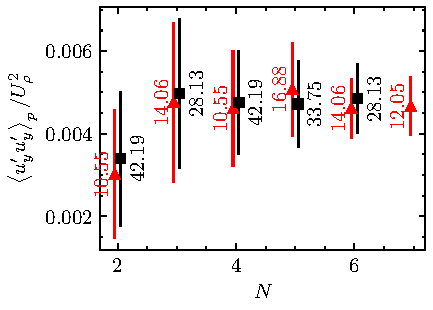
\includegraphics[height= 0.3\textwidth]{image/VALIDATION/N_and_delta/PA_UpUp.pdf}
    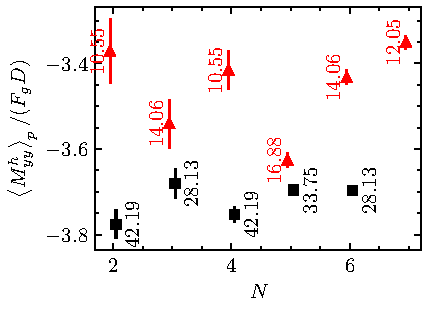
\includegraphics[height= 0.3\textwidth]{image/VALIDATION/N_and_delta/Mh.pdf}
    \caption{(left) Fluids phase averaged fluctuation tensor.
            (right) Particular average of the first moment tensor, where $F_g$ is the buoyancy force applied on one droplet. 
            The numerical values displayed alongside the dots are the number of cells per diameter.}
    \label{fig:VALIDATION_Nd_2}
\end{figure}
Now, let's look at the behavior of more \textit{complicated} closure terms. 
\ref{fig:VALIDATION_Nd_2}(left) demonstrate that the vertical component of the pseudo turbulent tensor is parameter independent rather early, independently of the grid definition. 
This fact is rather surprising but notice that the standard deviation is quite high for small domain. 
On \ref{fig:VALIDATION_Nd_2}(right), we can examine the vertical component of the first moment closure term. 
It is found to be constant for all $N$, but rather inaccurate for coarse grids. 
Which makes sens since the first moment results from a local calculation of the stress over a droplet volume, unlike the other quantities which results from the averaged center of mass velocity of a droplet. 

As we have shown, the quantities presented converge for a number of droplets equivalent to $N = 4$ and $\delta = 25$. 
Thus, we validate our simulation in space, i.e. we made sure that our domain were wide enough to minimize the influence of the periodicity on our results, and in mesh definition. 
Nevertheless, at it is the number of realization that matter when carrying a particular average, it is interesting to look at the duration of the simulation.

\subsection{Time average convergence}

The aim of this study is to be able to identify the minimum required time (or number of time steps) to obtain a representative mean. 
In this set of results we made sure that all the simulations were carried for a time that is more than sufficient. 
Therefore, in this section, we observe the convergence of the mean of a quantity depending on the number of the sample of time taken through the simulation.
More specifically we define the cumulative mean of an already, space averaged quantity, $F$, as, 
$\bar{F}(t) = \int_{T_{start}}^{t} F dt$. 
Where we introduced the start of sampling time $T_{start}$, which correspond to the starting time at which we are gathering data. 
This time is chosen as the time it takes for the simulation to reach a statistically steady state.
In other worlds, it is the time it takes for the droplets to get from an inert ordered state ($t = 0$), to a fully random state, where the droplets reach their mean drifting velocity.
As, we could remark, from its high standard deviation, the most difficult quantity, difficult in the meaning that it doesn't converge rapidly, is the \textit{Reynolds} stress tensor averaged on the particular phase, namely $\pnavg{u'_yu'_y}$.
Thus, we will confirm the representativity of our simulations, by looking at the cumulative time average of this quantity. 
\begin{figure}
    \centering
    % 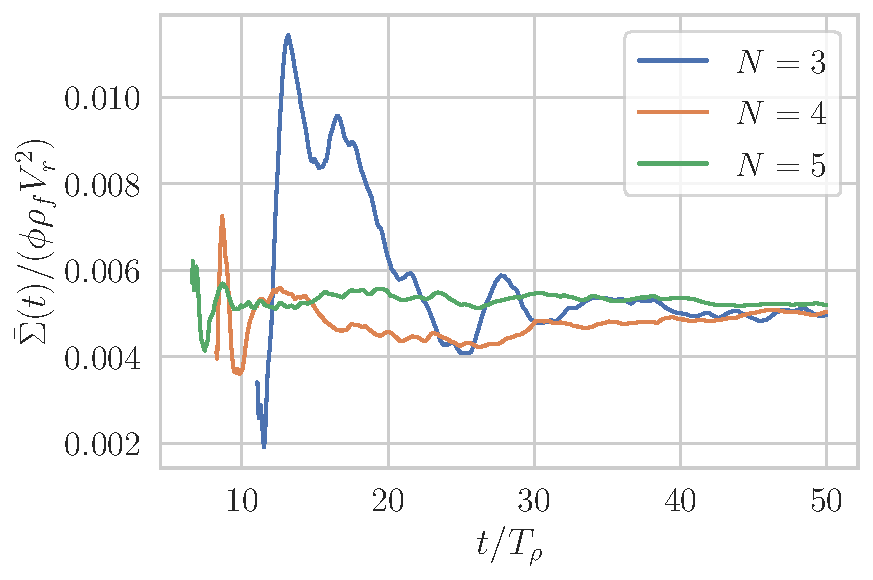
\includegraphics[height = 0.3 \textwidth]{image/VALIDATION/time/Sigma.pdf}
    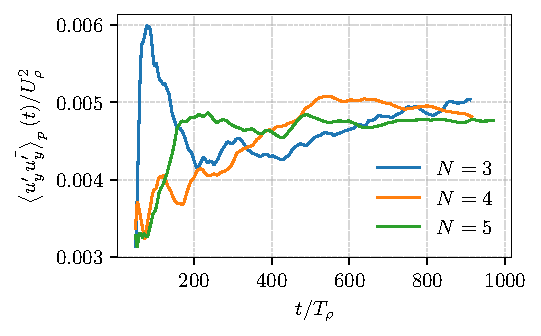
\includegraphics[height = 0.3 \textwidth]{image/VALIDATION/time/UpUp.pdf}
    \caption{Cumulative mean of the \textit{Reynolds} stress tensor. For $N = 3,4,5$ and $\delta = 25$, with $t/T_{start} = 10$.}
    \label{fig:VALIDATION_cumul_mean}
\end{figure}
From, \ref{fig:VALIDATION_cumul_mean}, it is apparent that the case where, $N=5$, has a faster convergent mean. 
Indeed, if we examine the picture, it is evident that the curve for $N=5$ reach a steady state earlier than the other ones. 
As a matter of fact, it can be perceived that the $N=5$ simulation reaches a steady mean at $t/T_\rho = 25$, while the other converge much latter. 
As a result, this study show, without surprise, that the result of the particular \textit{Reynolds} stress tends toward a steady mean faster for the simulation where $N=5$. 
In view of this it is interesting that for this range of \textit{Galileo} the time required to have significant results it $t/T_{\rho} \approx 110$, where we added the start time and $100$ inertial sampling time. 


\subsection{Asymptotic regime in low \textit{Galileo}}

Ideally we would like to cover a wide range of \textit{Galileo} numbers. 
Meaning that we need to reach both asymptotic regime, at low and high $Ga$ for any closure, if we suppose that such asymptotic regime exist. 
We limit our validation to the drag force or drift velocity closure term. 
In this section we show that in the limited range studied, i.e. $Ge \in [5,100]$, we cover enough \textit{Galileo} number to reach the low and high inertia asymptotic regime. 

First, it is interesting to see that the range of \textit{Galileo} number studied correspond to a wider range of \textit{Reynolds} numbers. 
Indeed, \ref{fig:Ga_Re} we clearly see that the computed \textit{Reynolds} numbers, based on the drift velocity, i.e. $Re = D (\cavg{\textbf{u}} - \davg{\textbf{u}}) \rho_f/\mu_f$, results in a wider range than the input \textit{Galileo} numbers. 
\begin{figure}[h!]
    \centering
    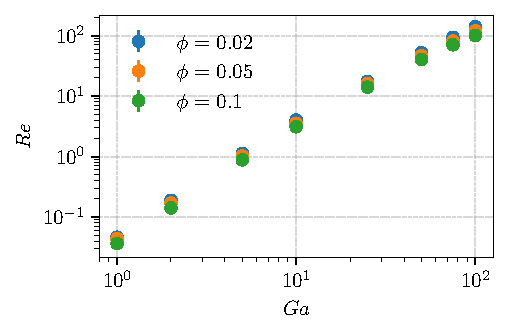
\includegraphics[height= 0.3\textwidth]{image/Dim_3/fCA/Re.pdf}
    \caption{\textit{Reynolds} number computed with the drift velocity, in terms of the \textit{Galileo} numbers.}
    \label{fig:Ga_Re}
\end{figure}
Thus, we cover both regime, inertial for $Re \approx 0.1$ and non-inertial with $Re \approx 100$. 
In order to investigate the different asymptotic regime of the drag force closure term, we plotted, in \ref{fig:f_u_f_rho}, the dimensionless drag force under two different form. 
In the first case (\ref{fig:f_u_f_rho}(left)) it is made dimensionless by the viscous material terms, namely,
\begin{equation*}
    \cavg{\textbf{f}^\mu} = \frac{\textbf{g} D^2\Delta \rho}{\mu_f |\cavg{\textbf{u}} - \davg{\textbf{u}}|}. 
\end{equation*} 
While in the other case it is made dimensionless with the inertial assumption, 
\begin{equation*}
    \cavg{\textbf{f}^\rho} = \frac{\textbf{g} D\Delta \rho}{\rho_f |\cavg{\textbf{u}} - \davg{\textbf{u}}|^2}. 
\end{equation*} 
\begin{figure}[h!]
    \centering
    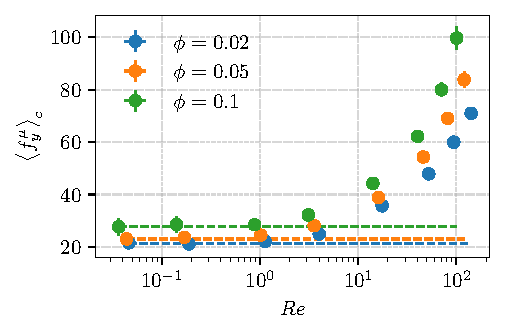
\includegraphics[height= 0.3\textwidth]{image/Dim_3/fCA/FH_Re_mu.pdf}
    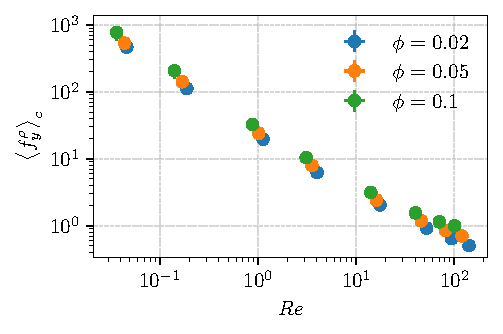
\includegraphics[height= 0.3\textwidth]{image/Dim_3/fCA/FH_rho_Re.pdf}
    \caption{(left) Non-inertial dimensionless vertical drag force term. 
             (right) Inertial dimensionless vertical drag force term. }
    \label{fig:f_u_f_rho}
\end{figure}
In \ref{fig:f_u_f_rho}(left) we can observe that $\cavg{\textbf{f}_\mu^*}$ tend to a constant value for approximately, $Re \le 1$, corresponding to a $Ga \le 5$.
Meaning, that we reach an asymptotic regime at $Ga=5$, and that it will probably tend to this same value at even lower $Re$ or $Ga$. 
However, as demonstrated by \ref{fig:f_u_f_rho} (right) the high inertial regime do not tend to a constant yet. 
Thus, no additional conclusion can be drawn so far for high inertial regime. 

In conclusion, in order to cover a wide enough range of \textit{Galileo}, we do not need to investigate $Ga<5$ since the lower \textit{Galileo} simulations, seems to behave proportionally to the case where $Ga = 5$. 
Regarding the high inertial regime, as we cannot really go above $Ga =100$ (due to the required mesh definition at higher $Ga$), we limit our study to $Ga =100$.  
Consequently, in the following simulation were carried though the range $Ga = [5,100]$, corresponding to $Re \in [1,100]$. 

\subsection{Statistical convergence}

\subsubsection{Pair PDF of presence}

In the next chapter we will see that the radial distribution function has a major importance in the closure problem. 
In order to be representative while reconstructing this function numerically, we need to gather enough sample of relative event of pairs of particles position. 
Thus, when $N$ increase, the number of particles realization of pairs of particles increase, thus we expect that $g(r)$ tends toward a constant function with increasing $N$. 
The question is, how many droplets per domain do we need so that this function is indeed representative (keeping the simulation time and time step constant) ? 
\begin{figure}[h!]
    \centering
    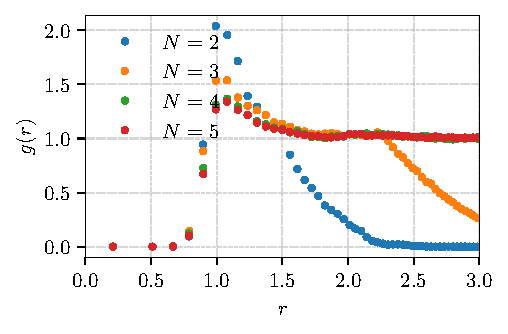
\includegraphics[height= 0.3\textwidth]{image/VALIDATION/fDist/g_r.pdf}
    \includegraphics[height= 0.3\textwidth]{image/VALIDATION/fDist/N_g_1.pdf}
    \caption{(left) Plot of the radial distribution function $g(r)$ for different $N$. 
             (right) Plot of the values of $g$ for $r =1$ in terms of the number of droplets inside the domain for different mesh definition. }
    \label{fig:g_r}
\end{figure}
On \ref{fig:g_r} (left), we see that the radial distribution function $g(r)$, tends to one with increasing $r$, which is exactly what we expect from a radial distribution function, thus it is a first validation. 
Moreover, the value of the radial distribution at $r\approx1$, is of a major importance since it is used in a closure models for the particular phase averaged stress in solid particle suspensions \citep{jackson2000dynamics}, it is also used in kinetic theory for the collision kernel modeling, \citep{fede2015monte}.
Therefore, \ref{fig:g_r} (right) we plotted the value of $g(r=1)$ for different mesh definition and number of particles per domain. 
It is evident that $g(1)$ reach a constant value above $N=4$ for a mesh definition $\delta = 25$. 

We established that the statistical distribution converged radially. 
Nevertheless, we would like to study the angular distribution in addition to the radial distribution.  
Thus, on \ref{fig:VALIDATION_fDrop_3} we show different 2D plots of this 2D distribution function. 
By comparing both plot it clearly indicates that this 2 dimensional distribution converge at $N=5$. 
\begin{figure}[h!]
    \centering
    % 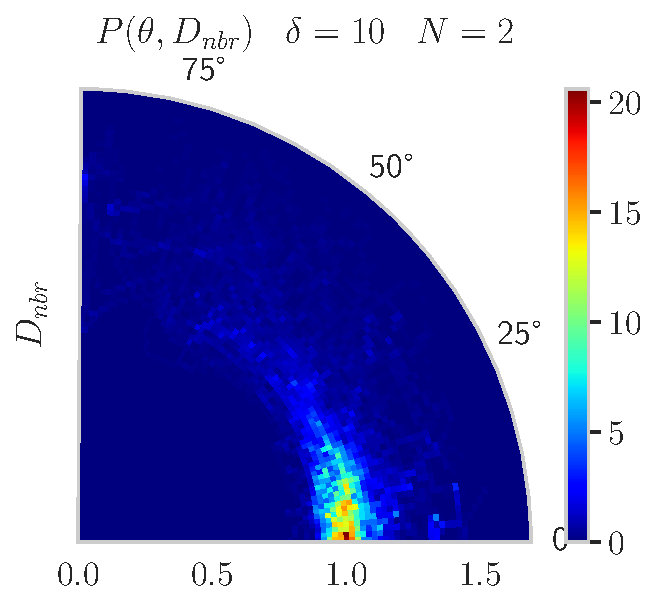
\includegraphics[height= 0.35\textwidth]{image/VALIDATION/fDrop/D_nbr_Theta_ndc_10_N_2.pdf}
    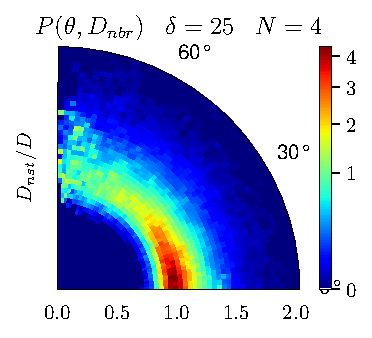
\includegraphics[height= 0.3\textwidth]{image/VALIDATION/fDrop/U_Theta_ndc_25_N_4.pdf}
    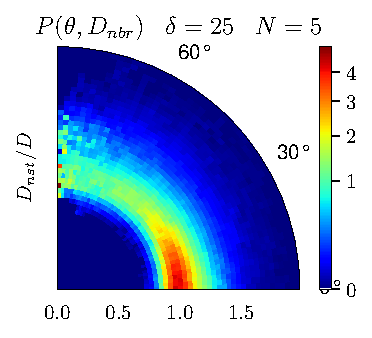
\includegraphics[height= 0.3\textwidth]{image/VALIDATION/fDrop/U_Theta_ndc_25_N_5.pdf}
    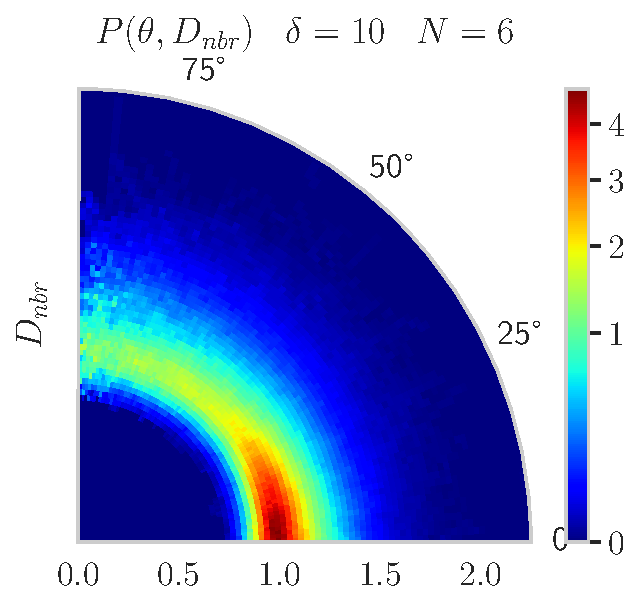
\includegraphics[height= 0.3\textwidth]{image/VALIDATION/fDrop/U_Theta_ndc_10_N_6.pdf}
    % 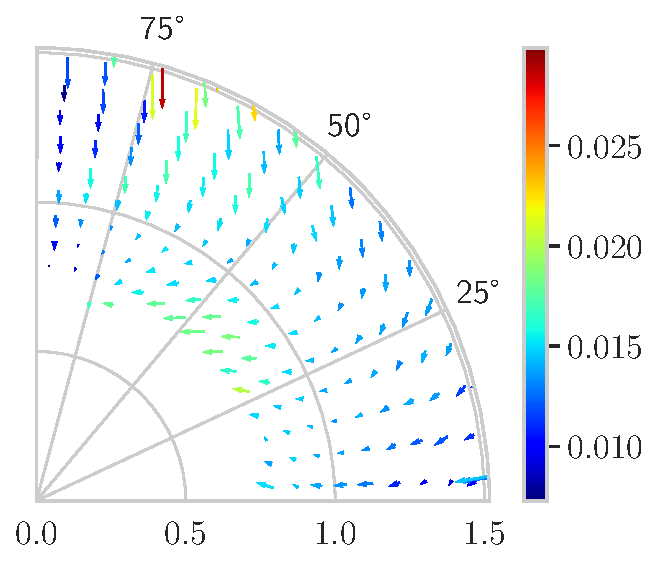
\includegraphics[height= 0.35\textwidth]{image/VALIDATION/fDrop/Dmin_Theta_Ur_uT_75_PHI_0_15.pdf}
    \caption{Radial distribution function of the nearest particle, $P(\theta, D_{nst}/D)$. 
    From $N=4$ (left) to $N=6$ simulations (right).}
    \label{fig:VALIDATION_fDrop_3}
\end{figure}
Indeed, if we look to the color bar of each plot and to the plot itself, we clearly see that the value of the PDF is the same for all $N$. 
Nevertheless, we can distinguish a small difference between $N=4$ and the others, even though it is small it deserves to be notified. 
Therefore, we consider a 2D distribution independence above a number of 64 ($N=4$) droplets per domain. 


\subsubsection{Influence of the mesh definition on nearest statistics}

Now that the required number of sample is fixed need to check out the influence of the mesh definition at the inter particle scale. 

To do so we propose to study the following a case with the following dimensionless numbers. 
We set $Ga = 75$ to be in the most disadvantageous situation. 
\begin{align}
    Ga = 75
    & \phi = 0.1
    & \mu_r =0.1 
    & \rho_r = 1.1
    & Bo = 1 
\end{align}
Finlay we test three number of cells quality, $\delta > 10$, $\delta > 25$, $\delta > 35$. 


\section{Experimental design}

From the previous few sections, we were able to identify and select relevant dimensionless parameters 
to be studied in the next chapters. 
They were deduced from parameters independence depicted in the previous few sections.
They are summaries in \ref{tab:parameters2}.
\begin{table}
    \caption{Ranges of the studied dimensionless parameters.}
    \centering
    \begin{tabular}{|c|c|c|c|c|c|c|} \hline
        $Ga$ &
        $\phi$ & 
        $Bo$ &
        $\rho_r$ &
        $\mu_r$ &
        $T_{max}/T_g$ &
        $\Delta t/T_{\sigma}$\\ \hline
        5-100
        &0.01-0.15
        & 1 
        & 1.1
        & 0.1-10
        & 500
        & 10 \\\hline
    \end{tabular}
    \label{tab:parameters2}
\end{table}
Most of the parameters have been discussed above. 
Regarding, $\phi$ we limited our study below $0.15$ because above this value bubbles or droplets instantaneously coalesce and the flow isn't dispersed anymore. 
Below $\phi =0.01$ the required domain is too wide, thus the simulations would be too expensive to carry, even though lower volume fraction would have been of interest. 
The \textit{Bond} number has been determined based on the shape of the particles. 
Indeed, we know that for extremely low $Bo$ a droplet will remain spherical. 
Thus, as for our application (see introduction of \ref{chap:avg}) we aim for spherical droplets, i.e. \textit{Bond} numbers, we need to seek for convergence toward low $Bo$. 
And as it will be shown in the results, for $Bo =1$, and this range of $Ga$, the particles remain spherical, thus we reach this asymptotic regime for low $Bo$. 
The density ratio $\rho_r = 1.1$ correspond to the ratio of our application. 
Regarding, the viscosity ratio our application (oil /water) is at $\mu_r=0.1$, but we allow our selves to explore a wider range event though we won't be able to describe entirely this dimension. 
The time of the simulation is scaled on the inertial time, $T_\rho$, as the simulations are mostly driven by inertial effect (i.e. $Ga \in [5,100]$). 
The value of $500$ inertial time has been validated empirically as can be shown by the accuracy of the previous results. 
The time step has been scaled with the capillary time in order to sample several time steps in a period of deformation of a droplet. 

In brief, the numerical parameters together with the physical ones are well validated.
Therefore, in the following chapters we carry out simulations in the restricted ranges of the parameters depicted \ref{tab:parameters2}.


\section{Numerical methodology}
\label{sec:methodo}

This section outlines the approach employed for performing simulations to achieve statistically steady states in the context of a rising mono-disperse suspension of droplets within a fully periodic domain.
We start by presenting the relevant physical parameters, followed by an overview of the numerical methods employed.
Finally, we detail the methodology implemented for collecting statistical data on microstructure, which will be presented in the following sections.

%In this section we expose the strategy employed to conduct statistically steady state simulations of rising mono-disperse suspension of droplets in a fully periodic domain. 
%We start by introducing the physical parameter, followed by a description of the numerical methods.
%Lastly, we detail the methodology adopted to collect statistics about microstructure, which are presented in the next sections.

%The source code used to perform the DNS is entirely open source.
%The simulations are running within the \texttt{Basilisk C} framework, (see \href{http://basilisk.fr}{basilisk.fr}), which is an extension of the C programming language, adapted for the solution of partial differential equations on Cartesian meshes. 
%Note that this section is complemented by the wiki page, \href{http://basilisk.fr/sandbox/fintzin/Rising-Suspension/RS.c}{RS.c}, where the reader can access the source code used to conduct the DNS, as well as comments and notes to help comprehension. 

\subsection{Problem statement}

We investigate numerically the dynamics of homogeneous mono-disperse emulsions subject to buoyancy forces in a fully periodic domain. 
The dispersed and continuous phases are considered Newtonian fluids defined by viscosity $\mu_d$ (resp. $\mu_f$) and density $\rho_d$ (resp. $\mu_f$).
Throughout this work, the subscript $_d$ and $_f$ indicate properties belonging to the dispersed and continuous phases, respectively. 
The interface between both fluids is considered infinitely thin, free of impurities, and characterized by a constant surface tension $\gamma$. %with a coefficient  is assumed. 
The density and viscosity will be considered constant in each phase.
In dimensionless form, this problem is completely characterized by six dimensionless parameters:  the viscosity and density ratio, $\lambda = \mu_d / \mu_f$ and $\zeta = \rho_d / \rho_f$,  
the \textit{Galileo} number, 
\begin{equation*}
    Ga =\frac{\sqrt{\rho_f(\rho_f - \rho_d) g d^3}}{\mu_f},
\end{equation*}
the \textit{Bond} number, 
\begin{equation*}
    Bo =\frac{(\rho_f - \rho_d) g d^2}{\gamma},
\end{equation*}
the number of droplets per domain $N_b$, and the dispersed phase volume fraction $\phi$. 
Here, $d$ represents the diameter of a sphere with the same volume as the droplets and $g$ denotes the acceleration of gravity.
The \textit{Galileo} number measures the strength of the buoyancy forces relative to the viscous forces, whereas the \textit{Bond} number evaluates the ratio between buoyancy and capillary forces. 

%To provide a brief overview of the range of interest for these numbers in an industrial context, let us consider the example of a vegetable oil/water system.
%In most liquid-liquid system encountered in industrial processes the diameter of the droplets lies in the range $d = [50 \mu \text{m}, 3 \text{mm}]$. To provide order of magnitude of the quantities of interest let us consider the example of a vegetable oil dispersed in water. The density and viscosity of the continuous phase are approximately $\rho_f = 1000 \text{kg/m}^3$ and $\mu_f = 10^{-3} \text{Pa.s}$, respectively. The density and viscosity of the dispersed phase are close to $\rho_d = 900 \text{kg/m}^3$ and $\mu_d = 10^{-2} \text{Pa.s}$, respectively.
%We consider the gravitational acceleration on earth, thus $g= 9.81 \text{m.s}^{-2}$.
In most liquid-liquid systems encountered in industrial processes, the droplet diameters typically range from 10 micrometers to a few millimeters. To illustrate the order of magnitude of the relevant quantities, consider a scenario where vegetable oil is dispersed in water. The continuous phase (water) has a density of approximately $\rho_f = 1000 \text{kg/m}^3$ and a viscosity of about $\mu_f = 10^{-3} \text{Pa.s}$. In contrast, the dispersed phase (vegetable oil) has a density close to $\rho_d = 900 \text{kg/m}^3$ and a viscosity around $\mu_d = 10^{-2} \text{Pa.s}$.
The surface tension of the oil/water system is approximately $\gamma = 0.05 \text{N.m}^{-1}$. The maximum allowable volume fraction is set at $\phi = 0.2$. Beyond this value, particles tend to coalesce easily, leading to a loss of the dispersed flow topology.%The maximum volume fraction is set to $\phi = 0.2$, indeed above such $\phi$ particles coalesce easily and the topology of the flow cannot be considered as dispersed anymore. %\citep{de2015gouttes}. 
\begin{table}[h!]
    \centering
    \caption{Dimensionless parameters of a water/oil system.}
    \begin{tabular}{|c||c|c|c|c|c|}
        \hline&$Ga$&$Bo$&$\phi$&$\lambda$&$\zeta$\\ \hline
        \hline Oil/Water&$[0.35,160]$&$[10^{-5};10^{-1}]$&$<0.2$&$10$&$0.9$\\ \hline
    \end{tabular}
    \label{tab:parameters_exp}
\end{table}
\ref{tab:parameters_exp} gives the corresponding dimensionless parameters.  
Notice that the \textit{Bond number} is relatively low, indicating that the droplets are nearly spherical in these processes.
Following \ref{tab:parameters_exp}, to approach real-life applications, we conducted DNS for four volume fractions, specifically $\phi = 0.01,0.05,0.1,0.2$.
In contrast to most previous studies, we keep the number of droplets constant while changing the volume fraction $\phi$. 
We then modify the domain size $\mathcal{L}$ accordingly. 
This introduces another dimensionless parameter of interest: $\mathcal{L}/d$, which measures the confinement of the particles within the finite numerical domain. 
This parameter is purely determined by $\phi$ and $N_b$, and will thus be refereed as a \textit{secondary parameter}.

As mentioned, the \textit{Bond} numbers of our targeted application is very low.
Therefore, the \textit{Bond} number is set to $Bo = 0.2$, and it will stay constant throughout this study.
DNS with lower \textit{Bond} numbers become excessively expensive due to the restrictive capillary time step constraint. 
However, we assert that for $Bo \leq 0.2$, the droplet shape essentially remains spherical, at least for small \textit{Galileo} numbers. 
Additionally, the ratio between inertia and surface tension forces is given by the \textit{Weber} number, 
\begin{equation*}
    We = \frac{\rho U^2d}{\gamma}%\frac{Bo \cdot Re^2}{Ga},
\end{equation*}
%where $Re = \frac{\rho_f d U}{\mu_f}$ is the Reynolds number based on 
where $U$ is the relative velocity which is the difference between the dispersed phase velocity and the continuous velocity.%drift velocity $U$ which is the difference between the dispersed phase velocity and the bulk velocity.
%Values of \textit{Reynolds} numbers for each DNS are provided in \ref{ap:slip_vel} (\ref{fig:Reall}). 
Extreme values of $We$ reached in these simulations are displayed in \ref{tab:simulations}. 
It is clear that for $We=0.6$, we might expect some deformations; nevertheless, in most cases, $We$ stays below these values. 
Consequently, whether in the viscous or inertial regimes, the droplets are expected to remain spherical according to the values of $Bo$ and $We$.
This statement is verified in appendix \ref{ap:deformation}.%will be verified in \ref{sec:microstructure}. 

%Density and viscosity ratio of droplets in real life applications are reported in \citet[Figure 1.]{balla2020effect}.
%As depicted in \citet[Figure 1.]{balla2020effect}, the viscosity and density ratio of fluid-fluid systems range between, $\lambda \in [10^{-4} : 10^4]$ and $\zeta \in [10^{-1} : 10^1]$, respectively. 

The study's primary objective is to investigate the microstructure through the nearest particle pair distribution function.
Thus, obtaining a sufficient number of DNS samples is crucial to ensure statistical convergence. 
Also, the physical quantities measured in the simulations must remain independent of the domain size. 
Therefore, we use a number of particles per domain of $N_b = 125$, roughly what \citet{hidman2023assessing} used for their DNS of fully-periodic buoyant rising bubbles.
Moreover, each DNS lasts for a time: $t^*_\text{end} = 1500 \sqrt{d/g}$.
% It is shown in \ref{ap:validation} that these parameters  are sufficient to obtain well converged statistics.  
\begin{table}[h!]
    \centering
    \caption{Dimensionless parameter range investigated in this work.}
    \begin{tabular}{|ccccccc|ccc|}\hline
        \multicolumn{7}{|c|}{Primary parameters}&\multicolumn{3}{|c|}{Secondary parameters}\\\hline\hline
        $Ga$&$Bo$&$\phi$&$\lambda$&$\zeta$&$N_b$&$t^*_\text{end}$&$\mathcal{L}/d$&$Re$&$We$\\ \hline
        $5\rightarrow 100$&$0.2$&$1\% \rightarrow 20\%$&$10$ \& $1$&$0.9$&$125$&$1500$&$6.7\to 18.7$&$10^{-1}\to 170$&$10^{-4}\to 0.6$\\ \hline
    \end{tabular}
    \label{tab:simulations}
\end{table}
This study presents DNS results with dimensionless parameters in ranges outlined in \ref{tab:simulations}.
In summary, we investigated $5$ \textit{Galileo} number $Ga = 5,10,25,50,100$, $4$ different volume fractions $\phi = 0.01,0.05,0.1,0.2$, and two viscosity ratios $\lambda =1,10$ with $Bo = 0.2$ and $\zeta = 0.9$. %In this study we restrict our attention to a single density ratio, $\zeta = 0.9$.
%Regarding the viscosity ratio, we accomplished DNS for 2 different values, namely $\lambda = 1,10$.
%Lastly, to explore the effect of inertia on the microstructure, the \textit{Galileo} number will vary within the range $Ga \in [5,100]$.
This makes a total of $40$ representative simulations of $N_b = 125$ droplets which last for $t= 1500 \sqrt{d/g}$. 
\subsection{Numerical method}

In this problem, the governing equations consist of the one-fluid formulation of the mass and momentum equation, with an additional transport equation for the dispersed phase indicator function. 
We recall their form here, 
\begin{align}
    \pddt \rho+ \div(\rho\textbf{u})
    &= 0,\\
    \label{eq:dt_urho}
    \pddt (\rho \textbf{u})
    + \div (\rho  \textbf{u} \textbf{u} - \bm\sigma)
    &= (\avg{\rho} - \rho)\textbf{g}
    + \textbf{f}_\gamma,\\
    \label{eq:dt_C}
    \pddt C + \textbf{u}\cdot\grad C  
    &= 0,
\end{align}
% \tb{mettre le link navier stokes solver et faire ca pour le reste }
which are the mass, momentum and colors function transport equation, respectively. 
The scalar fields $C$, represents the color function, which range between $0$ and $1$ to indicate the proportion of fluid and dispersed phase, respectively. 
We introduced the fluid velocity vector $\textbf{u}$ and the Newtonian stress tensor $\bm{\sigma} = -p \textbf{I} + \mu (\grad \textbf{u}+ \grad \textbf{u}^\dagger)$ where $p$ is the pressure fields and $^\dagger$ represents the transpose operator.
Note that the material properties, $\rho$ and $\mu$, take the value of the phases in presence, following the arithmetic average : $\rho = (1-C)\rho_f + C \rho_d$ and $\mu = (1-C)\mu_f + C \mu_d$. 
In our case the arithmetic mean turns out to perform better compared to the harmonic mean, which is often used to interpolate the viscosity for bubbly flows \citet{hidman2023assessing,innocenti2020direct}.
More details about this choice is provided in \ref{ap:validation} (\textit{Case 1.}). 
The capillary force is defined as, $\textbf{f}_\gamma =\textbf{n} \gamma \div \textbf{n} $, where \textbf{n} is the normal at the interface.
Following  \citep{bunner2002dynamics}, we incorporated the artificial body force term, $\avg{\rho}\textbf{g}$, on the right-hand side of \ref{eq:dt_urho}, to maintain a zero-averaged velocity throughout the entire numerical domain.  

To solve these equations we first initialized $125$ spherical droplets within a cubic domain with fully periodic boundary condition. 
We used the open source code \url{http///basilisk.fr} to discretize the governing equations in a multigrid solver. 
The Navier-Stokes equations are discretized with a centered scheme.
The two-phase flow solver uses the Volume of Fluid (VoF) method. 
The interfaces between the droplets and the carrier fluid is reconstructed using the Piecewise Linear Inter-face Calculation or PLIC method \citet[Chapter 5.]{tryggvason2011direct}.
Regarding the treatment of the surface tension force term we refer the reader to \citet{popinet2018numerical} for more details. 
The Basilisk solver has been validated extensively, in the framework of bubbly flow. 
Most of the previous studies \citep{hidman2023assessing,innocenti2020direct} recommend a grid definition of $\Delta/d \ge  30$, where $\Delta$ is the grid spacing. 
In \ref{ap:validation} we carried a mesh independence study and demonstrate that a grid spacing of $\Delta = d/30$ is also suitable in our context.
For readers seeking more detailed information about the solvers, we recommend the wiki pages : \href{http://basilisk.fr/src/navier-stokes/centered.h}{centered.h}, \href{http://basilisk.fr/src/tension.h}{tension.h} and \href{http://basilisk.fr/src/poissson.h}{poissson.h} where he can find the source code of the Navier-Stokes, surface tension and multigrid solver used in this work, respectively. 

With the VoF method droplets and bubbles may experience premature coalesce.
For a detailed discussion on this issue, see  \citet[Appendix B]{innocenti2020direct}.
However, in this work, it is imperative to conserve a specific (mono-disperse) population of droplets over time to accumulate sufficient statistics about the microstructure.
To tackle this issue we present in the next section a novel algorithm which prevent coalescence between droplets, while maintaining a reasonable cost. 






\subsection{The \texttt{no-coalescence.h} algorithm}

In previous studies various methods have been used to avoid coalescence. 
One method is to increase artificially the surface tension coefficient at the interface contact points, as demonstrated in the recent study of \citet{hidman2023assessing}.
% This method seems highly efficient, in terms of simplicity and computational expenses. 
However, it remains unclear if the physical behavior of the droplets interactions is well captured due to the introduction of artificial forces. 
Additionally, its applicability for denser emulsions, up to $\phi = 0.2$, remains uncertain. 
\citet{balcazar2015multiple} developed a multiple-marker level-set method to prevent coalescence, while \citet{zhang2021direct} used a multi-VoF method. 
The latter method consists in assigning to each droplet a different color function so  that the interfaces are reconstructed independently when droplets are in close contact.
Since the representations of the interfaces are independent, droplets in contact never coalesce.  
The latter method may be suitable for our objectives, however, it can be quite expensive as it requires solving a transport equation for each tracer, with one tracer assigned per droplet, meaning $125$ tracers in our case. 
\citet{karnakov2022computing} developed a multi-VoF method which requires a fixed number of tracers for an arbitrary number of droplets.
This approach allows multiple non-touching droplets to belong to the same field, which makes it more efficient than the previous study.
Although this approach shares the same basic principle with the one used here, i.e. coloring adjacent droplets with different colors to avoid coalescence, it differs in term of computational methods. 
In the following we present our methodology that as implemented in the \texttt{Basilisk} framework. 

The challenge here is to assign a tracer to every adjacent droplets to prevent numerical coalesce, while minimizing the number of tracers to reduce computational cost. 
This recalls the famous \textit{Four color map theorem} \citep{appel1977solution} which essentially states that : 
\enquote{every map can be color using only four colors, so that two neighboring region are different colors}. 
In our case, this theorem implies that for any 2D configuration only four VoF tracer are necessary to avoid coalescence\footnote{It is worth noting that for a bi-periodic domain, seven colors are required due to the torus-like topology.  }. 
Therefore, leveraging the \textit{Four color map theorem}, one might be able to significantly reduce the number of VoF tracers required.
Note however that the optimal coloring problem is originally a static problem that need to be solved only once. 
In our case, droplets move around over time thus transforming the static problem into a time-dependent problem. 
Furthermore finding the optimal coloring is known to be difficult (the problem is {\em NP-complete}) and solving it at each timestep would be too expensive.

Note also that in three-dimensions the \textit{Four color map theorem} has no equivalent.
For example, an arbitrary large number of rectangular blocks in 3D-space can all touch each other, requiring an arbitrary large number of colors to differentiate the adjacent blocks\citep{magnant2011coloring}. 
We are not aware of an extension of the coloring problem to arrangements of spheres in 3D. 
Nevertheless, it is reasonable to assume that the number of tracers required to avoid coalescence is significantly smaller than the number of droplets.
Consequently, since we cannot determine the optimal coloring configuration based on theoretical grounds, we opt to assign the tracers to each droplet following the empirical strategy detailed below.

The development of the \texttt{no-coalesce.h} algorithm was initiated in the PhD. thesis of \citet{mani2021numerical}.
The latest version of this algorithm can be found on the basilisk wiki page : \href{http://basilisk.fr/sandbox/fintzin/Rising-Suspenion/no-coalescence.h}{no-coalescence.h}.
Before  diving into a step-by-step description of this algorithm we need to introduce another key feature used in these simulations, which is the \href{http://basilisk.fr/src/tag.h}{tag.h} algorithm. 
It is an adaptation of the \textit{painter}'s algorithm, but optimized using the multigrid solver of \texttt{Basilisk}. 
Its purpose is to assign different scalars values to each cell belonging to different regions, with the regions being delimited by the different droplets' interfaces. 
For instance, on \ref{fig:images} (left) we can see two blue regions corresponding to two different drops.
We can notice that both are assigned with two different values, $1$ and $2$, which are identified using the \texttt{tag.h} algorithm. 
It is then straightforward to obtain the droplet properties, such as its center of mass, by carrying numerical integration on the VoF field considering only the cells having a specific tag value, which corresponds to a given droplet.  
% In general, we are able to differentiate droplets' domain, belonging to the same tracer thanks to the \texttt{tag.h} algorithm.


We define the $i^\text{th}$ color function as $C_i$ for $i =1,2,\ldots,N(t)$, where $N(t)$ is the total number of tracers used in a simulation at time $t$.
The color function introduced previously is now defined as, $C = \sum_{i=1}^{N(t)} C_i$. 
Note that $N(t)$ is time-dependent since the number of tracers may increase during the simulation as droplets get closer to one another.
The simplified workflow of the algorithm follows these four steps : 
\begin{enumerate}
    \item[\textit{Step 1}.] Check if within a tracer field $C_i$, the droplets are possibly too close to each other. 
    The \textit{near contact} criterion that determines if the droplets are too close is defined using a $5$ by $5$ cells stencil which verifies the following conditions : 
    (1) If the color function $C_i = 0$ at the center of the stencil. 
    (2) And if $C_i > 1$ for two opposite cells in the stencil. 
    In this case two different regions might be in close contact.
    A sketch of this situation is given in \ref{fig:criterion}.  
    \item[\textit{Step 2}.] 
    If (\textit{Step 1}.) is true for the tracer $C_i$, we must verify if we indeed identified two different regions in near contact, and not just a single region close to itself, such as in \ref{fig:diagram} (right). 
    Therefore at this step  we apply the \texttt{tag.h} algorithm.
    \item[\textit{Step 3}.] Re-use the \textit{near contact} criterion of (\textit{Step 1}.) by requiring in addition that the cells must belong to two different tag groups. 
    At this stage the situation in \ref{fig:criterion} (left) would be true, while the situation on \ref{fig:criterion} (right) would be false. 
    We therefore identified all the droplets / region that are indeed too close to each other. 
    \item[\textit{Step 4}.] 
    Find a new tracer field $C_n$, with which we could set the region/droplets that are in near contact. 
    At this stage, it is essential to identify the list of tracer $C_j$ already in contact with the region to be replaced. 
    For example, in \ref{fig:criterion} (left), the droplet on the right is clearly adjacent to a region with tracer $C_j$, in which case $C_n$ must satisfy $n \neq i,j$. 
    Therefore, any $n$ in $1, 2, \ldots, N(t)$ are suitable candidates as long as this situation is avoided. 
    If the droplet is already adjacent to every tracer $C_j$ in the simulation, for $j = 1, 2, \ldots, N(t)$, we create a new tracer $C_n$ with $n = N(t)+1$ and assign the drop to this tracer field.
\end{enumerate}
\begin{figure}
    \centering
    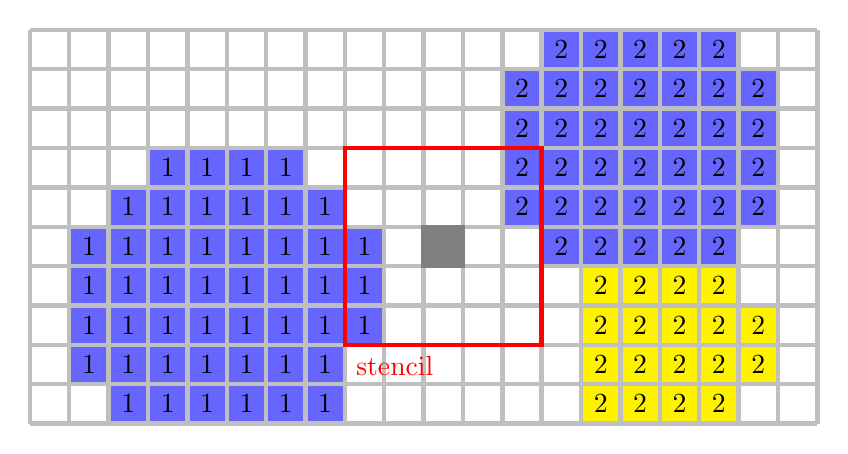
\begin{tikzpicture}[scale=0.5,ultra thick]
        % Define grid dimensions
        \def\nRows{10}
        \def\nCols{20}
        \pgfmathsetmacro\nRowsm{\nRows-1}
        \pgfmathsetmacro\nColsm{\nCols-1}

        \foreach \row in {0,...,\nRowsm} {
            \foreach \col in {0,...,\nColsm} {
                \pgfmathsetmacro\distance{veclen(\col-4.356, \row-2.65)};
                \pgfmathparse{\distance < 4 ? "blue" : "white"}
                \edef\colour{\pgfmathresult};
                \ifthenelse{\equal{\colour}{blue}}{                    
                    \fill[\colour!60!white] (\col, \row) rectangle ++(1,1);
                    \node (num) at (\col +0.5,\row+0.5){1};
                }
            }
        }

        \foreach \row in {0,...,\nRowsm} {
            \foreach \col in {0,...,\nColsm} {
                \pgfmathsetmacro\distance{veclen(\col-15, \row-6.2)};
                \pgfmathparse{\distance < 3.5 ? "blue" :"white"}
                \edef\colour{\pgfmathresult};
                \ifthenelse{\equal{\colour}{blue}}{
                    \fill[\colour!60!white] (\col, \row) rectangle ++(1,1);
                \node (num) at (\col +0.5,\row+0.5){2};
                }
            }
        }

        \foreach \row in {0,...,\nRowsm} {
            \foreach \col in {0,...,\nColsm} {
                \pgfmathsetmacro\distance{veclen(\col-15.62, \row-1.5)};
                \pgfmathparse{\distance < 2.5 ? "yellow" :"white"}
                \edef\colour{\pgfmathresult};
                \ifthenelse{\equal{\colour}{yellow}}{
                    \fill[\colour] (\col, \row) rectangle ++(1,1);
                    \node (num) at (\col +0.5,\row+0.5){2};
                }
            }
        }
        % Define grid size
        \pgfmathsetmacro\gridSize{1}
        
        \foreach \row in {0,...,\nRows} {
            \draw [gray!50] (0,\row*\gridSize) -- (\nCols*\gridSize,\row*\gridSize);
        }
        % Draw vertical grid lines
        \foreach \col in {0,...,\nCols} {
            \draw [gray!50] (\col*\gridSize,0) -- (\col*\gridSize,\nRows*\gridSize);
        }
        % Draw drop shape
        \draw[red] (8,2)node[below right]{stencil} rectangle +(5,5); % Draw the rectangular base
        \filldraw[gray] (10,4) rectangle +(1,1);
    \end{tikzpicture}    
    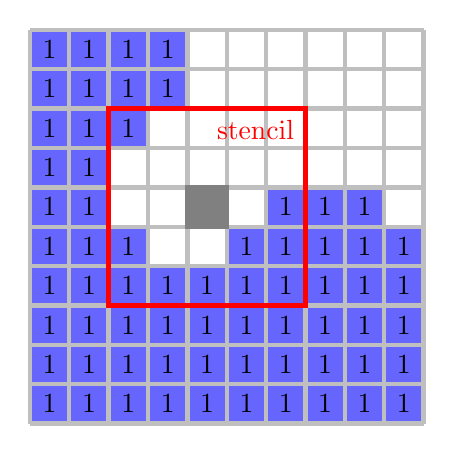
\begin{tikzpicture}[scale=0.5,ultra thick]
        % Define grid dimensions
        \def\nRows{10}
        \def\nCols{10}
        \pgfmathsetmacro\nRowsm{\nRows-1}
        \pgfmathsetmacro\nColsm{\nCols-1}

        \foreach \row in {0,...,\nRowsm} {
            \foreach \col in {0,...,\nColsm} {
                \pgfmathsetmacro\distance{veclen(\col, \row-2)};
                \pgfmathparse{\distance < 3.5 ? "blue" :"white"}
                \edef\colour{\pgfmathresult};
                \ifthenelse{\equal{\colour}{blue}}{
                    \fill[\colour!60!white] (\col, \row) rectangle ++(1,1);
                \node (num) at (\col +0.5,\row+0.5){1};
                }
            }
        }

        \foreach \row in {0,...,\nRowsm} {
            \foreach \col in {0,...,\nColsm} {
                \pgfmathsetmacro\distance{veclen(\col-7, \row-2)};
                \pgfmathparse{\distance < 3.5 ? "blue" :"white"}
                \edef\colour{\pgfmathresult};
                \ifthenelse{\equal{\colour}{blue}}{
                    \fill[\colour!60!white] (\col, \row) rectangle ++(1,1);
                    \node (num) at (\col +0.5,\row+0.5){1};
                }
            }
        }
        \foreach \row in {0,...,\nRowsm} {
            \foreach \col in {0,...,\nColsm} {
                \pgfmathsetmacro\distance{veclen(\col-5, \row)};
                \pgfmathparse{\distance < 3.5 ? "blue" :"white"}
                \edef\colour{\pgfmathresult};
                \ifthenelse{\equal{\colour}{blue}}{
                    \fill[\colour!60!white] (\col, \row) rectangle ++(1,1);
                    \node (num) at (\col +0.5,\row+0.5){1};
                }
            }
        }
        \foreach \row in {0,...,\nRowsm} {
            \foreach \col in {0,...,\nColsm} {
                \pgfmathsetmacro\distance{veclen(\col, \row-9)};
                \pgfmathparse{\distance < 3.5 ? "blue" :"white"}
                \edef\colour{\pgfmathresult};
                \ifthenelse{\equal{\colour}{blue}}{
                    \fill[\colour!60!white] (\col, \row) rectangle ++(1,1);
                    \node (num) at (\col +0.5,\row+0.5){1};
                }
            }
        }
        % Define grid size
        \pgfmathsetmacro\gridSize{1}
        
        \foreach \row in {0,...,\nRows} {
            \draw [gray!50] (0,\row*\gridSize) -- (\nCols*\gridSize,\row*\gridSize);
        }
        % Draw vertical grid lines
        \foreach \col in {0,...,\nCols} {
            \draw [gray!50] (\col*\gridSize,0) -- (\col*\gridSize,\nRows*\gridSize);
        }
        % Draw drop shape
        \draw[red] (2,3) rectangle +(5,5)node[below left]{stencil}; % Draw the rectangular base
        \filldraw[gray] (4,5) rectangle +(1,1);
    \end{tikzpicture}    
    \caption{Sketch of two situations were the \textit{near contact} criterion is true. 
    The background grid represents the cells within the numerical domain. 
    The dark blue area represents the cells where $C_i > 0$.
    The yellow area represents the cells where the tracer $C_j > 0$ for $j\neq i$. 
    The numbers represent the values of the $Tag$ scalar field within each tracer.
    The $5$ by $5$ cells red rectangle represents the stencil zone which iterates over all cells of the domain.  
    %  where the center of the stencil (gray square) must respect $C_i = 0$. 
    (left) Two droplets in contact since we have two opposite cells in the stencil with $C_i > 0$ and $C_i=0$ at the center.
    And the mentioned cells belong to two different regions so that (\textit{Step 3}) is also validated.  
    (right) A near contact is observed since we have two opposite cells in the stencil with $C_i > 0$ and $C_i=0$ at the center, however in this case we do not verify the second criterion of \textit{Step 3} which requires two different tags values. 
    }
    \label{fig:criterion}
\end{figure}
These four steps are executed at each simulation time step and for each tracer $C_i$ with $i = 1, 2, \ldots, N(t)$.
Following this procedure, we ensure that all adjacent droplets are using different tracers, which ultimately prevents coalescence. 

Having $N(t)$ tracers requires some modifications to the aforementioned governing equations. 
Specifically, instead of solving \ref{eq:dt_C}, we solve $N(t)$ transport equations, one for each $C_i$.
Likewise, the surface tension force is computed as the sum of the contributions from each $C_i$ and reads
\begin{align*}
    \pddt C_i + \textbf{u}\cdot\grad C_i = 0,
    \ \  \ \ \forall i = 1,2,\ldots N(t),\\
    \textbf{f}_\gamma 
    = \sum_{i=0}^{N(t)} \gamma \kappa_i \grad C_i
\end{align*}
where $\kappa_i$ is the numerical approximation of the curvature of the interface of field $C_i$, which is computed following the same method employed for a single tracer. 

\ref{fig:diagram} (left) shows a snapshot of a simulation at an arbitrary time $t^* = 100 \sqrt{g/d}$. 
The droplet interfaces are colored by the indices of their respective tracer. 
In this simulation at that time, no more than 3 colors are needed to avoid coalescence.
On \ref{fig:diagram} (right) we display the value of $N(t)$ in term of the dimensionless simulation time for various volume fractions $\phi$ at $Ga = 50$ and  $\lambda = 1$. 
We observe that for the entire simulation, no more than 3 tracers were needed for the dilute emulsion ($\phi = 0.01$) and up to 7 for the denser regime ($\phi = 0.2$). 
Although our algorithm might not be optimized, it brings sufficient efficiency for our needs. 
Indeed, \ref{tab:performance} reports the time spent by each function during a simulation. 
It is observed that the \texttt{no-coalesce.h} algorithm accounts for approximately $4\%$ of the total computational time of a simulation. 
As for the \texttt{tag.h} algorithm, its cost is around $2\%$, which is also reasonable.
In comparison, the \texttt{poisson.h} solver is about $13\%$ of the simulation time. 
The advection of VoF tracers is about $7\%$ which is relatively high but still reasonable.
To reduce the cost related to the \texttt{no-coalesce.h} algorithm we believe that further developments, which are referenced at \href{http://basilisk.fr/sandbox/fintzin/Rising-Suspenion/no-coalescence.h}{no-coalescence.h}, are still doable and could be useful for future studies.
\begin{figure}[h!]
    \centering
    \begin{tikzpicture}
    \node (img) at (0,0) {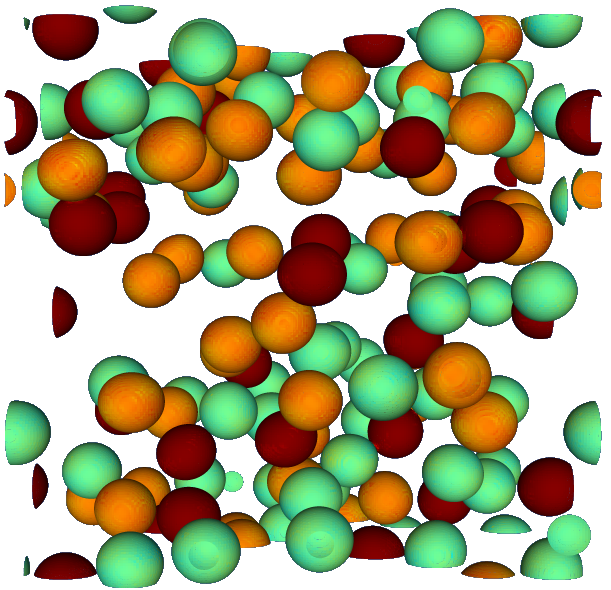
\includegraphics[width = 0.4\textwidth]{image/VoF2.png}};
    \node (img) at (0.4\textwidth,-0.01\textwidth) {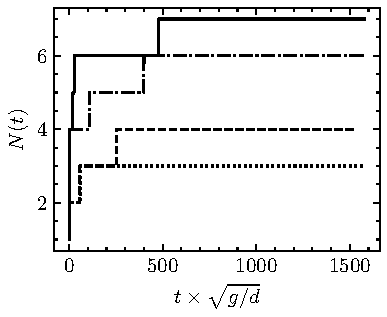
\includegraphics[width = 0.4\textwidth]{image/HOMOGENEOUS_NEW/CA/NVoF_vs_t_Ga_50_l_1.pdf}};
    \end{tikzpicture}
    \caption{
    (left) Snapshot of a DNS with $\phi = 0.05$, $\lambda = 1$, $Ga = 50$ with the interface of the droplets colored by the index of the tracers.
    (right) Number of tracers $N(t)$ as a function the dimensionless time.
    Four different volume fractions are displayed : (dotted line) $\phi = 0.01$, (dashed line) $\phi = 0.05$ (dash dotted line) $\phi = 0.1$ (solid line) $\phi = 0.2$ at $Ga = 50$ and $\lambda = 1$. 
    }
    \label{fig:diagram}
\end{figure}


In order to validate our numerical methodology, we have compared our numerical results to the experiments of \citet{mohamed2003drop} where they experimentally study the impact of a single drop on a flat interface of the same fluid. %, while recording the positions of the interfaces.
It is found that the multi-VoF method captures remarkably well the position of interfaces, even with a poor description of the liquid film between these interfaces.
Additionally, we argue that the mesh independence study conducted in \ref{ap:validation} (Case 3) substantiates the accuracy of the DNS, as the dynamics of interaction do converge with  reasonable errors for a grid resolution of $\Delta/d = 30$. 
Overall, we used an optimized multi-VoF method, enabling us to perform DNS with a maximum of 7 tracers in the densest scenario.
 








\section{Additional details on the algorithms}
\tb{make small intro here}
\section{Additional details on the algorithms}
In addition to the developments above, implementing the algorithm required further modifications to the \texttt{Basilisk C} source code. 
Specifically, since computing the closure terms involves extensive tensor algebra, we implemented a new macro in the \texttt{Basilisk C} compiler that enables users to write code directly using Einstein summation convention. 
Additionally, we introduced a new standard struct, \texttt{mat3}, alongside the existing \texttt{coord} struct. 
The \texttt{mat3} struct represents second-order tensors, while \texttt{coord} is used for vectors. 
By incorporating these two structs into the Basilisk C language, we developed an automated macro allowing \texttt{MPI} reduction directly on \texttt{coord} and \texttt{mat3} structures. 

Overall, we provided all necessary tools in the Basilisk pre-compiler to enable programming directly with tensor algebra.
Below is a brief description of the main functionality of the so-called, \texttt{Einstein\_sum}$(\ldots)$ macro.

\subsection{Einstein summation notation}

This \href{http://basilisk.fr/src/ast/einstein_sum.h}{header file} contains the functions related to the Einstein summation macro implemented by the $\texttt{Basilisk C}$ preprocessor. This macro allows the user to write tensor algebra in index notation using $\texttt{Basilisk C}$ code. The syntax follows the famous \href{https://en.wikipedia.org/wiki/Einstein\_notation}{Einstein summation convention}.

\subsubsection{ Mathematical definitions}

Let us give the basis of the Einstein summation convention through the example of a simple scalar product between two second-order tensors in $3D$ space. In mathematics and physics, it is customary to write second-order tensors as $\textbf{A} = \sum_{i,j = 1}^3 A_{ij} \bm e_i\bm e_j$ where $\bm e_i$ and $\bm e_j$ are basis vectors in $3D$ space and $A_{ij}$ is the component of the tensor $\textbf A$ projected on the vectors $\bm e_i\bm e_j$. In tensor notation the inner product between two arbitrary second-order tensors: $\textbf{A}$ and $\textbf{B}$, can be written as $\textbf{C} =  \textbf{A}\cdot\textbf{B}$. If the basis is orthonormal, the components of the tensor $\textbf C$ are given by
$$ C_{ij} = \sum_{k=1}^3 A_{ik} B_{kj}.$$
Since the summation operator can be quite cumbersome in the Einstein summation convention we rewrite this operation as
$$ C_{ij} = A_{ik} B_{kj} $$
where the summation over $k$ from $1$ to $3$ is implicit.
We took the example of a simple scalar product, nevertheless note that this notation extends to any tensor operations which can be much more complex.   
Therefore, to remove any ambiguity in the Einstein summation notation, one has to follow the following rules:
1. each index can appear at most twice in any term,
2. repeated indices are implicitly summed over,
3. each term must contain identical non-repeated indices.

For example the expression: $M_{ij}v_iv_j$ is valid and indicate a double summation over $i$ and $j$, 
while the rexpression $M_{ij}v_ju_j$ is ambigous since the index $j$ appears $3$ times. 
For a more complete and rigourous definition of the Einstein summation convention we recommand the Wikipedia page: \href{https://en.wikipedia.org/wiki/Einstein\_notation}{Einstein summation convention}.

\subsubsection{ User interface}

To write a scalar product in $\texttt{Basilisk C}$ one needs first to define vector and second-order tensor-like structures. The default vector structure is the `coord` struct. The second or higher-order structures must be defined by the user. 
\begin{lstlisting}[language=C]
typedef struct {
coord x,y,z;
} mytensor;
mytensor A,B,C; 
\end{lstlisting}
Note that the name `mytensor` is arbitrary. However, the name of the structure members must be $x$, $y$ and $z$. Following the Einstein summation convention the scalar product introduced in the previous paragraph can be written in $\texttt{Basilisk C}$ as
\begin{lstlisting}[language=C]
einstein_sum(i,j,k) {
  C.i.j = A.i.k*B.k.j; 
}
\end{lstlisting}
With this macro, the preprocessor of $\texttt{Basilisk C}$ interprets all lines of code within the braces as tensor operations. The letters given within the parenthesis indicate the indices on which the Einstein summation takes place. In this case a summation will be applied on the index $k$ and permutations will be performed on the indices $i$ and $j$. 
To verify that the $\texttt{Basilisk C}$ preprocessor gives the desired results, one can precompile the $\texttt{Basilisk C}$ file with the command line
\begin{lstlisting}
qcc -source my_file.c
\end{lstlisting}
The results of the precompilation stored in \texttt{\_my\_file.c} will be
\begin{lstlisting}[language=C]
{
  C.x.x = A.x.x*B.x.x+ A.x.y*B.y.x+ A.x.z*B.z.x;
  C.x.y = A.x.x*B.x.y+ A.x.y*B.y.y+ A.x.z*B.z.y;
  C.x.z = A.x.x*B.x.z+ A.x.y*B.y.z+ A.x.z*B.z.z;
  C.y.x = A.y.x*B.x.x+ A.y.y*B.y.x+ A.y.z*B.z.x;
  C.y.y = A.y.x*B.x.y+ A.y.y*B.y.y+ A.y.z*B.z.y;
  C.y.z = A.y.x*B.x.z+ A.y.y*B.y.z+ A.y.z*B.z.z;
  C.z.x = A.z.x*B.x.x+ A.z.y*B.y.x+ A.z.z*B.z.x;
  C.z.y = A.z.x*B.x.y+ A.z.y*B.y.y+ A.z.z*B.z.y;
  C.z.z = A.z.x*B.x.z+ A.z.y*B.y.z+ A.z.z*B.z.z;
}
\end{lstlisting}
Note that the preprocessor duplicated the lines for each permutation of $i$ and $j$ and applied a summation over the index $k$. This macro also applies to $\texttt{Basilisk C}$ vector fields (such as the velocity field `u.x[]`) and any other user-defined structures with members named $x$, $y$ and $z$.

For higher-order rank tensors one can note that these expressions become quite cumbersome.
It is for that reason that the \texttt{einstein\_sum} macro has been created. 
For more examples one can check the test file \href{einstein\_sum.c}{/src/test/einstein\_sum.c}.

\subsubsection{Specific cases}

As long as the user follows the rules mentioned above, the desired result will be obtained. 
However, the \texttt{einstein\_sum} macro is somewhat more permissive than the original rules of the convention. 
For example the code
\begin{lstlisting}[language=C]
U.i = M.i.j*u.j*v.j;
\end{lstlisting}
which is **not defined correctly** will still be compiled, and in $2D$ will give
\begin{lstlisting}[language=C]
U.x = M.x.x*u.x*v.x + M.x.y*u.y*v.y;
U.y = M.y.x*u.x*v.x + M.y.y*u.y*v.y;
\end{lstlisting}
The use of C functions within the macro is also allowed. 
Let `function(args)` be an arbitrary C function. 
Then the expression, 
\begin{lstlisting}[language=C]
U.i = function (M.i.j*u.j*v.j);
\end{lstlisting}
will be expanded to
\begin{lstlisting}[language=C]
U.x = function (M.x.x*u.x*v.x + M.x.y*u.y*v.y);
U.y = function (M.y.x*u.x*v.x + M.y.y*u.y*v.y);
\end{lstlisting}

The summation is applied at the lowest level of the expression where all the indices that must be summed over are present. 
Here the summation takes place inside the parenthesis since all indices \texttt{j} are contained within them. 

A useful example of the use of a function is the computation of the L2 norm of the second-order tensor $\textbf C$
\begin{lstlisting}[language=C]
L2 = sqrt (C.i.j*C.i.j);
\end{lstlisting}
Lastly, if no equality sign is identified, the preprocessor will not perform any summation operations. It will only carry the permutation on the current line of code. For example if one wants to print the content of a tensor one may write 
\begin{lstlisting}[language=C]
einstein_sum (i,j) {
  fprintf (stderr, "%g\n", C.i.j);
}
\end{lstlisting}
which gives in $2D$
\begin{lstlisting}[language=C]
  fprintf (stderr, "%g\n", C.x.x);
  fprintf (stderr, "%g\n", C.x.y);
  fprintf (stderr, "%g\n", C.y.x);
  fprintf (stderr, "%g\n", C.y.y);
\end{lstlisting}


In summary the \texttt{einstein\_sum} macro follows the following steps:
\begin{enumerate}
    \item  It Identifies if a given line of code is an assignment expression with a "=" sign or not. 
    \begin{enumerate}
    \item If it is, it identifies the indices on the right and left-hand side of the expression. 
       It then carries a summation over the indices that appear only on the right-hand side. 
    \item If it is not an equality, it does nothing at this step. 
    \end{enumerate}
    \item  It then copies the lines of codes and carries permutations on the indices present on the line (excluding the one that has been summed over). 
    \item Steps 1. and 2. are repeated for all lines within the macro. 
\end{enumerate}
Note that these steps do not follow the original Einstein summation convention rules. 
Therefore, some expressions may be ambiguous and the user is advised to always check for the pre-compiler results using \texttt{qcc -source my\_file.c} before using the code.

\subsection{Performing  MPI reduction on list of \texttt{coord} and \texttt{mat3} types}

The implementation of the reduction feature is available on \texttt{Basilisk} website by tracking the Darcs update authored by me.

No further comments are necessary regarding this development, as the functionality mirrors that of the existing \texttt{reduction()} macro.



% \section{Concluding remarks}

Now that we have all the tools required to perform DNS, we can proceed to study the closure terms in the next few chapters. Although we may be able to extend the theoretical closures presented in \ref{chap:daniel2}, the reader must be reminded that, with these DNS, we are still confined to a very specific scenario. 
The effects of polydispersity and non-homogeneous flow regimes cannot be studied within this setup and will therefore be disregarded in the closure modeling. 
This further highlights the complexity and the actual resources needed to numerically complete the closure of the Navier-Stokes equations.







\subsubsection{The reduction macos ? }

%%%%%%%%%%%%%%%%%%%%%%%%%%%%%%%%%%%%%%
%%%%%%%%%%%%%%% PART 3 %%%%%%%%%%%%%%%
%%%%%%%%%%%%%%%%%%%%%%%%%%%%%%%%%%%%%%
% \part{Buoyancy driven motion of non-coalescing inertial drops}

\chapter{Microstructure modeling with nearest particle statistics}
\localtableofcontents

\section{Introduction}
\section{Introduction}



\begin{enumerate}
    \item[Intro : ]
    Buoyancy-driven droplet flows are encountered in many chemical engineering processes such as gravity separators, liquid-liquid extractors, etc. The usual engineering practice to model such facilities is to make use of the averaged Navier-Stokes equations and population balance equations. 
    \item[Why is it interesting :]
    However, these methods necessitate closure laws and a deep understanding of particle pair statistics.
    Especially, closures laws are in fact microstructure dependent. 
    Therefore, in an objective to understand to physics these terms it is primordial to understand the microstructure and why it is like so. 
    \item[bibliography : ]
    Previous authors investigated the microstructure of bubbly flows. 
    \citet{bunner2002dynamics} reported the creation of horizontal raft for rising  spherical bubbles. 
    \citet{bunner2003effect} demonstrated taht due to wake trapping effect deformable bubbles have a tendency to align horizontally. 
    In a more recent study \citet{zhang2021direct} also found the creation of horizontal layers of particles. 
    Regarding the solid particles other studies have been conducted for the sedimentation of spheres \citet{shajahan2023inertial}, and they found a high probability of particle pair on  the side of the particle of reference.     
    \item[What is still needed :]
    None, of these studies focus on droplets' suspension. 
    So no closure are available. 
    Additionally, none of them proposed an algorithm to avoid coalesce. 
    \item[What good if i new :]
    An algorithm to prevent coalesce would allow us to perform DNS for arbitrary long time with a fixed population of droplets. 
    In addition to providing data for the closure terms appearing in averaged models, the simulations are of great interest to understand and describe the microstructure of suspensions. 
    \item[introduce the plan :]
    Therefore, within a multiscale strategy, we perform tri-periodic Direct Numerical Simulations (DNS) of monodisperse buoyancy driven suspension of drops.
    In this work we present a concise analysis of the microstructure by analyzing the \textit{Nearest Particle Statistics} recently revisited by \citet{zhang2021ensemble}. 
    We start in \ref{sec:methodo} to present the DNS methodology. 
    Then, we introduce quickly the \textit{nearest particle statistics}.
    In \ref{sec:microstructure} we present an analysis of the microstructure geometry and identify structure such as layers and cluster with respect to the dimensionless parameters. 
    Then, in \ref{sec:time} we describe the relevant timescale of the flow. 

\end{enumerate}

\section{Nearest particle statistics}
\label{sec:nearest}

To study the emulsions' microstructure, we chose to adopt the \textit{nearest particle statistics} framework recently revisited by \citet{zhang2021ensemble}.
We now recall some definitions of the \textit{nearest particle statistics} averaging procedure. 
For further details, readers are encouraged to refer to \citet{zhang2023evolution} on which this work mostly relies.

\subsubsection*{Theoretical framework}
Let $P(\FF)$ be the probability density function that describes the probability of finding the flow in the configuration $\FF$, where $\FF = (\lambda_1,\lambda_2,\lambda_3,\ldots)$ is a finite set of all the parameters describing the initial flow configuration.
% \footnote{We assume that the flow can be described by a finite number of parameters related to both phase.}. 
Then, we define $d\mathscr{P} = P(\FF)d\FF$ as the probable number of realizations in the incremental region of the flow' phase space, $d\FF$ around $\FF$.
Additionally,  $\textbf{x}_i(t,\FF)$ and $\textbf{x}_j(\FF,t)$ refers to the Lagrangian position vectors of the particles $i$ and $j$, respectively. 
We also introduce the age of the interaction, denoted as $a$, which represents the time elapsed since two particles became nearest neighbors.
Then, the nearest pair probability density function is given by,
\begin{equation}
    P_{nst}(\textbf{x},\textbf{r},a,t)= 
    \int \sum_{i}^{N_b}\delta(\textbf{x}-\textbf{x}_i)
    \sum_{j\neq i}^{N_b}\delta(\textbf{x}+\textbf{r}-\textbf{x}_j) 
    \delta(t+a-t_c^{ij}) 
    h_{ij} d\mathscr{P},
    \label{eq:P_nstij}
\end{equation}
where we introduced the function $h_{ij}$, which equals $1$ if and only if particle $j$ is one of the nearest neighbors of particle $i$, and $h_{ij} = 0$ otherwise. 
$t_c^{ij}(\FF,t)$ represents the time at which particles $i$ and $j$ became nearest neighbors. 
Formally, we have $a = t - t^{ij}_c(\FF,t)$.
Consequently, $P_{nst}(\textbf{x},\textbf{r},t,a)$ is the probability of having a particle center of mass located at $\textbf{x}$ at time $t$ with it nearest neighbor at $\textbf{x}+\textbf{r}$ given that the pair of particles have been nearest neighbors since $a$ time.
Note that $P_\text{nst}(\textbf{x},\textbf{r},t,a)$ is related to the number density $n_p(\textbf{x},t)$ through the relationship, 
\begin{equation*}
    \int_0^\infty 
    \int_{\mathbb{R}^3}
     P_\text{nst}(\textbf{x},\textbf{r},t,a) d\textbf{r} da = n_p(\textbf{x},t). 
    \label{eq:Pnst}
\end{equation*}
This establishes consistency between the nearest particle statistic and kinetic theory. 


Furthermore, $\textbf{w}_{ij}(t,\FF) = \textbf{u}_j(t,\FF) - \textbf{u}_i(t,\FF)$ represents the relative velocity between the particles $i$ and $j$, at time $t$ in the configuration $\FF$. 
With, $\textbf{u}_i(t,\FF)$ and $\textbf{u}_j(t,\FF)$, the Lagrangian center of mass velocities of the particles $i$ and $j$, respectively. 
The formal expression of the ensemble average of such a quantity is given by,
\begin{equation*}
    \textbf{w}^\text{nst}_p P_{nst}(\textbf{x},\textbf{r},t,a)
    = 
    \int \sum_{i}^{N_b}\delta(\textbf{x}-\textbf{x}_i)
    \sum_{j\neq i}^{N_b}\delta(\textbf{x}+\textbf{r}-\textbf{x}_j) 
    \delta(t+a-t_c^{ij}) 
    \textbf{w}_{ij}
    h_{ij} 
    d\mathscr{P}.
    \label{eq:q_nstij}
\end{equation*}
Following this definition, $\textbf{w}^\text{nst}_p(\textbf{x},\textbf{r},t,a)$ is the averaged relative velocity between the nearest pairs, conditioned on the presence of a particle at $\textbf{x}$ and time $t$, with its nearest neighbor at $\textbf{x}+\textbf{r}$ with age $a$. 
The physical meaning of such a field will be further investigated in \ref{sec:velocity}. 
The superscript $^\text{nst}$ indicates that $\textbf{w}_{ij}(\FF,t)$ is ensemble-averaged conditionally on the presence of the nearest neighbor, and the subscript $_p$ indicates that it is at the origin a Lagrangian property. 
More generally, $\textbf{w}_{ij}(t,\FF)$ can be replaced by any particle properties, an example used in this work is $\textbf{u}_i(\FF,t)$.
In this case, $\textbf{u}^\text{nst}_p(\textbf{x},\textbf{r},t,a)$ represents the conditionally-averaged particle phase velocity, given the presence of a particle at \textbf{x} and time $t$, with its nearest neighbor position at $\textbf{x}+\textbf{r}$ with age $a$. 

Since, we model a statistically steady and homogeneous configuration, the variables $\mathbf{x}$ and $t$ seem to have no interest. 
Nevertheless, we argue that $\mathbf{x}$ and $t$ indicate the dependence of the averaged quantities on the global flow parameters, $Ga$, $\phi$, $Bo$, $\zeta$, and $\lambda$.
Therefore, it is essential to retain $\mathbf{x}$ and $t$ in our notation. 



\subsubsection*{Numerical sampling}

To reconstruct all these statistics from the DNS, we treat each simulation time step  as an independent flow configuration, denoted as, $\FF$. 
Under this assumption, the ensemble average operators can be rewritten as :
\begin{equation}
    \int  d\PP\ldots
    = \frac{1}{E}\sum_\FF^\text{E} \ldots 
    \label{eq:discrete_ensemble_average}
\end{equation}
where $E$ is the total number of events, which, in our case, corresponds to the total number of time steps simulated.  
When performing conditional average based on the position of the nearest neighboring particle, the methodology is slightly different. 
To reconstruct a quantity such as $\textbf{w}^\text{nst}_p(\textbf{x},\textbf{r},t,a)$ we gather all the relative velocity $\textbf{w}_{ij}(t;\FF)$ from the simulation and store them in $n$ intervals of ages $\Delta a_k$, and relative positions $\Delta \textbf{r}_k$ for $k = 1,\ldots, n$.
Then, we apply the discrete ensemble average on $\textbf{w}_{ij}(t;\FF)$ for each group independently.
Formally, we write, 
\begin{equation}
    \textbf{w}^\text{nst}_p(\textbf{x},t,\Delta\textbf{r}_k,\Delta a_k)
    = \frac{1}{E_k} 
    \sum^{E_k}_{\FF_k} 
    % \sum_i^{N_b}
    % \sum_{j\neq i}^{N_b}
    \textbf{w}_{ij}(t;\FF_k)
    % h_{ij}
    % \text{\;\;  with  \;\;}
    % \FF_k = \{\FF; \textbf{r}(\FF)\in\Delta \textbf{r}_k, a(\FF)\in  \Delta a_k\}
    \label{eq:vec_cond}
\end{equation}
where $\FF_k$ correspond to the events were the nearest particle pair $i$ and $j$ respects $\textbf{r},a \in \Delta \textbf{r}_k ,\Delta a_k$.
$E_k$ is the total number of events fulfilling these constraints. 
Finally, we obtained an approximation of $\textbf{w}^\text{nst}_p(\textbf{x},\textbf{r},t,a)$ which takes the intervals, $(\Delta\textbf{r}_i,\Delta a_i)$ as input.
At some point, it will be useful to study the averaged relative velocity, conditioned on the age or on the radial distance, independently. 
Therefore, in a more general way if $p$ is a scalar property with $\Delta p_k$ its $n$ intervals, we can define the $p$-conditionally averaged relative velocity as, 
\begin{equation}
    \textbf{w}^\text{nst}_p(\textbf{x},t,\Delta p_k)
    = \frac{1}{E_{k}} 
    \sum^{E_{k}}_{\FF_{k}}  
    % \sum_i^{N_b} 
    % \sum_{j\neq i}^{N_b}
    \textbf{w}_{ij}(t;\FF_k)
    % h_{ij}
    % \text{\;\;  with  \;\;}
    % \FF_k = \{\FF; p(\FF)\in\Delta p_k\}
    \label{eq:scalar_cond}
\end{equation}
In this definition, $\FF_{k}$ corresponds to all the events where the nearest pair $i$ and $j$ respect the condition, $p \in \Delta p_k$, and $E_{k}$ represents the total number of events where $p\in\Delta p_k$. 

It is clear that to obtain representative averaged quantities, the number of events $E_k$ per intervals must be consequent. 
For 2D-conditioned quantity such as \ref{eq:vec_cond}, we estimated that $100$ samples per bins were sufficient to obtain qualitative results. 
Consequently, the plots exposed in \ref{sec:velocity} have been generated by averaging the quantity of interest (velocity fields, age of interaction) with a minimum threshold of $E_k = 100$ samples for each bin.
Regarding the scalar-conditioned fields such as in \ref{eq:scalar_cond}, we gathered $E_k = 1000$ sample per bins to obtain an accurate and quantitative results. 
Lastly, regarding the sampling, we collected data for each Lagrangian quantity every $10$ simulation time steps. 
The simulation time step is determined either by a Courant Friedrichs Lewy (CFL) condition or by the capillary time step, depending on the dimensionless numbers involved.
On average, $200,000$ time steps are performed during a simulation with $N_b = 125$ droplets. This results in a total number of $E = 2,500,000$ samples. In \ref{ap:validation} (\textit{Case 3}), we demonstrate that our statistics are well-converged.



\section{Microstructure}
\label{sec:microstructure}
This section presents an analysis of the microstructure based on the nearest neighbor probability density function. 
%age included nearest pair probability density function  $P_\text{nst}(\textbf{x},\textbf{r},t,a)$ and on .


%After identifying the different forms of the microstructure with respect to the dimensionless parameters, we introduce a general and concise way to quantify it.
By definition, $P_\text{nst}(\textbf{r}|\textbf{x},t)$ does not require symmetry with respect to the variable $\textbf{x}+\textbf{r}$ and \textbf{x}, as is the case for classical particle-pair distribution functions. 
Nevertheless, it turns out that $P_\text{nst}$ possesses a nearly-symmetric distribution, such that  $P_\text{nst}(r,\theta)\approx P_\text{nst}(r,- \theta)$ as demontrated below.
\begin{figure}[h!]
    \centering
    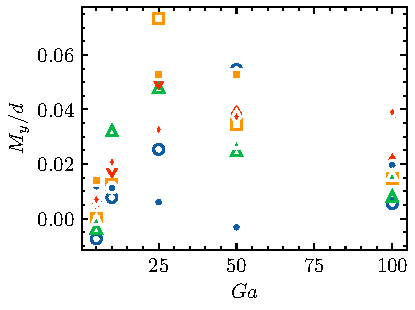
\includegraphics[height = 0.3\textwidth]{image/HOMOGENEOUS_NEW/PA/Ry.pdf}
    \caption{ Dimensionless first moment of the nearest particle pair distribution in the direction of gravity $M_y/d$. 
    ($\pmb\bigcirc$) $\phi = 0.01$; ($\pmb\triangle$) $ \phi = 0.05$; ($\pmb\square$) $\phi = 0.1$ ($\pmb\lozenge$) $\phi = 0.2$.
    The hollow symbols correspond to $\lambda = 1$, the filled symbols to $\lambda = 10$.
    % For $r<d$ we arbitrarily set $P_\text{r}^\text{th} = 1$ so that the distribution can be visualized.
    % Black symbols represent the results of \citet{zhang2023evolution} for hard sphere suspension with $\phi = 0.016,0.056,0.134,0.262$  %$\phi = 0.0168,0.0565,0.1341,0.2622$ 
    % corresponding to $\pmb\times,\pmb +, \pmb\star , \pmb\triangledown$, respectively.
    }
    \label{fig:ap:RY}
\end{figure}
%This is demonstrated by \ref{fig:ap:RY} 
%where we can see that the first moment of $P_\text{nst}$, namely
We define the first moment of $P_\text{nst}$ as
\begin{equation}
 \textbf{M} = \int_{\mathbb{R}^3} \textbf{r} P_\text{nst}(\textbf{r}) d\textbf{r}.
\end{equation}
\ref{fig:ap:RY} illustrates the projection of $\textbf{M}$ along the direction of gravity. 
The relatively small but finite values of $M_y$ indicate that $P_\text{nst}$ exhibits a nearly symmetric distribution with respect to $\theta$.
Nevertheless, this indicates that the nearest neighbor is more likely to be located in the upstream direction. 
Note that this is consistent with the findings of \citet{zhang2023evolution}.
Even though this slight asymmetry might have its importance \cite{zhang2023evolution}, we discard it in this study. 
Therefore, we choose to show only the upper part of the distribution in the following plots, (displayed in \ref{fig:Pnst_low_Ga} and \ref{fig:Pnst_high_Ga}) since qualitatively it remains the same as the lower part.  
Additionally, in the discussion below, we refer to the sphere at the origin of the graphs, located at $\textbf{x}=0$, as the \textit{test particle}.%\textit{test particle} or the \textit{test particle}. 

\subsection{Low inertia regimes}
We begin with a detailed analysis of $P_\text{nst}$ at $Ga =10$, to investigate the influence of $\lambda$ and $\phi$ on the microstructure when inertial effects are small.
\begin{figure}[h!]
    \centering
    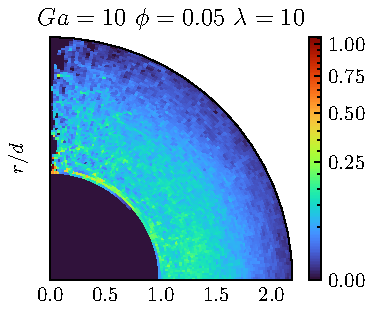
\includegraphics[height=0.21\textwidth]{image/HOMOGENEOUS_NEW/Dist/Pnst_l_10_Ga_10_PHI_0_05.pdf}
    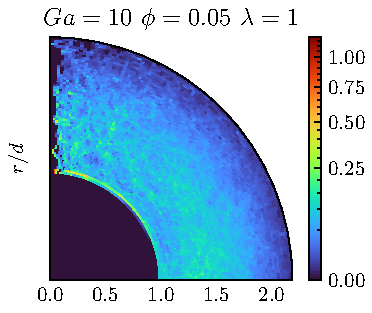
\includegraphics[height=0.21\textwidth]{image/HOMOGENEOUS_NEW/Dist/Pnst_l_1_Ga_10_PHI_0_05.pdf}
    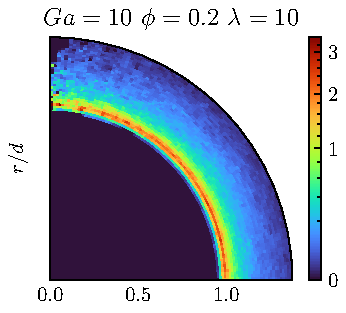
\includegraphics[height=0.21\textwidth]{image/HOMOGENEOUS_NEW/Dist/Pnst_l_10_Ga_10_PHI_0_2.pdf}
    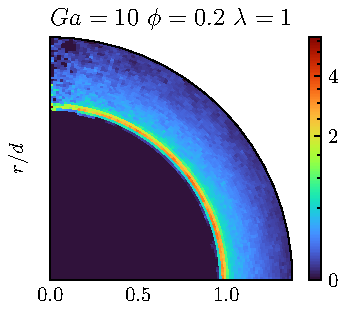
\includegraphics[height=0.21\textwidth]{image/HOMOGENEOUS_NEW/Dist/Pnst_l_1_Ga_10_PHI_0_2.pdf}
    \caption{Histogram of the probability density function, $P_\text{nst}(r,\theta)$, for low inertia $Ga = 10$.
    The color map represents the nearest pair distribution function. %the values of $P_\text{nst}$.
    The origin corresponds to the position of the \textit{test particle}.
    The dimensionless radial and azimuthal coordinates, $|\textbf{r}|/d$ and $\theta$, correspond to the nearest neighbor position.
    The vertical direction corresponds to the flow direction, which is also the axis of symmetry for $P_\text{nst}$.
    (left) Low volume fraction cases $\phi=0.05$ for $\lambda = 1,10$.
    (right) High volume fraction cases $\phi=0.2$ for $\lambda = 1,10$.
    }
    \label{fig:Pnst_low_Ga}
\end{figure}
The first observation from \ref{fig:Pnst_low_Ga} indicates that the likelihood of finding the nearest neighboring particle at an angle $\theta$ is uniform across all $\theta$.
This suggests that $P_\text{nst}$ is isotropic at these \textit{Galileo} numbers. We can observe that $P_\text{nst}$ is larger close to the \textit{test particle} ($r/d = 1$) in the high volume fraction cases than in the low volume fraction cases.
%If we compare the low volume fraction cases to the high volume fraction cases, we can observe that $P_\text{nst}$ is larger at near contact of the test particle ($r/d = 1$) in the latter case.
% For solid particles it is also common that pair distributions are more concentrated at the contact of the test particle for increasing $\phi$. 
In practice, if particles are more likely to be close to one another, it means that densely packed regions of particles are present in the flow.
This suggests that isotropic clusters, as represented in \ref{fig:scheme_clusters} (\textit{Case 2}), are likely to form in the present context. 
Regarding the effect of the viscosity ratio, $P_\text{nst}$ are very similar for both values of $\lambda$ except that for the highest volume fraction the region of highest probability is thinner for the lowest aspect ratio. 
Consequently, in this regime we find homogeneous microstructures at low $\phi$, and non-homogeneous but still isotropic microstructure (\textit{``clusters''}) at higher $\phi$. 


\subsection{High inertia regimes }
We now focus on the high inertia regimes ($Ga =80$).
In this situation, it is expected that the presence of particle wakes modify the interactions between particles \citep{yin2007}. 
\begin{figure}[h!]
    \centering
    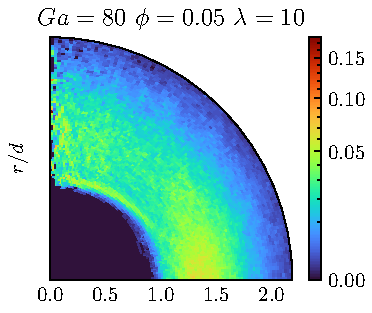
\includegraphics[height=0.205\textwidth]{image/HOMOGENEOUS_final/Dist/Pnst_l_10_Ga_80_PHI_0_05.pdf}
    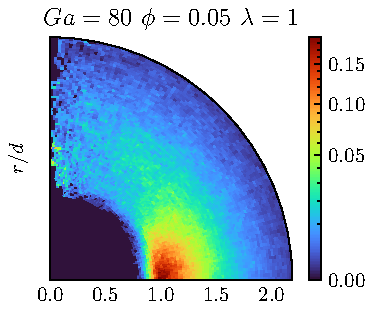
\includegraphics[height=0.205\textwidth]{image/HOMOGENEOUS_final/Dist/Pnst_l_1_Ga_80_PHI_0_05.pdf}
    \includegraphics[height=0.205\textwidth]{image/HOMOGENEOUS_final/Dist/Pnst_l_10_Ga_80_PHI_0_2.pdf}
    \includegraphics[height=0.205\textwidth]{image/HOMOGENEOUS_final/Dist/Pnst_l_1_Ga_80_PHI_0_2.pdf}
    \caption{Histogram of the normalized function $P_\text{nst}$ at high inertia $Ga = 80$.
    The color map represents the values of the nearest pair distribution function. %of $P_\text{nst}$.
    The origin corresponds to the position of the \textit{\textit{test particle}}.
    The dimensionless radial and azimuthal coordinates, $|\textbf{r}|/d$ and $\theta$, correspond to the nearest neighbor position.
    The vertical direction corresponds to the flow direction, which is also the axis of symmetry for $P_\text{nst}$.
    (left) Low volume fraction cases $\phi=0.05$ for $\lambda = 1,10$.
    (right) High volume fraction cases $\phi=0.2$ for $\lambda = 1,10$.}
    \label{fig:Pnst_high_Ga}
\end{figure}
%If we compare \ref{fig:Pnst_high_Ga} (right) with their counterparts from \ref{fig:Pnst_low_Ga} (right) we observe that $P^n_\text{r}$ becomes even larger at contact of the particles for $Ga=80$.
%Again, this could witness of the presence of clustering of particles. 
%In general, all $P_\text{nst}$ from \ref{fig:Pnst_high_Ga} exhibit some differences compared to the cases \ref{fig:Pnst_low_Ga}. 
%In the high inertial cases (\ref{fig:Pnst_high_Ga}), we can notice that $P_\text{nst}$ is larger on the sides of the \textit{test particle} for the iso-viscous emulsions ($\lambda = 1$).
Anisotropy in \ref{fig:Pnst_high_Ga} for $\lambda=1$ is particularly striking compared to \ref{fig:Pnst_low_Ga}. 
In the former, a higher concentration of particles is identified at $\theta \approx 0$, as seen in \ref{fig:Pnst_high_Ga}. 
A higher concentration of $P_\text{nst}$ around $\theta \approx 0$ indicates the presence of horizontal rafts of particles. 
In this case, the microstructure is non-homogeneous and anisotropic; this situation is illustrated in \ref{fig:scheme_clusters} (\textit{Case 3: ``layers''}). 
As the \textit{Galileo} number ($Ga$) increases and for low values of the viscosity ratio ($\lambda$), the probability of having neighbors on the horizontal plane of the \textit{test particle} increases. 
This leads to an increase in the anisotropy of the microstructure, which is more pronounced for low volume fractions. 
In contrast, the high-viscosity drops display an isotropic distribution of the nearest particles around the \textit{test particle}. 
This observation suggests the presence of isotropic clustering of particles.


%In comparison the high viscosity drops show an isotropic discitrbution of nearest particle around the \textit{test particle}. This could witness of the presence of isotropic clustering of particles.

%We do not observe a significant effect of the volume fraction on the anisotropy of the distribution.
%However, at this stage it remains unclear if increasing $\phi$ have a positive or negative impact on the anisotropy of the distribution. 

To illustrate the impact of $\lambda$ on the microstructure, \ref{fig:images} displays snapshots of two DNS at $\phi = 0.05$ and $Ga = 80$. 
As predicted by $P_\text{nst}$, we observe layers and particles in close contact for $\lambda = 1$, contrasting with the seemingly more evenly dispersed microstructure for $\lambda = 10$.
\begin{figure}[h!]
   \centering
   \includegraphics[width=0.45\textwidth]{image/HOMOGENEOUS_final/Ga_80_phi_005_l_1.png}
   \includegraphics[width=0.45\textwidth]{image/HOMOGENEOUS_final/Ga_80_phi_005_l_10.png}
   \caption{Snapshot of a simulation at $t^* = 200$ for $\phi=0.05$ and $Ga=80$.
   Color map : values of the vertical component of the velocity, field on the vertical plane defined by the equation $z=0$. 
   (left)  $\lambda = 1$.
   (right)  $\lambda = 10$.
   }
   \label{fig:images}
\end{figure}
In fact, for $\lambda = 10$, in \ref{fig:images} (right), we can still observe horizontal rafts of droplets or droplets rising side-by-side, but this effect is not as pronounced as for $\lambda = 1$. 
Drops with high viscosity ratios maintain a significant distance between other drops, which prevents the creation of structures such as droplet layers.
% This might be because of a higher vorticity around the viscous droplets.   
% As discussed in \citet{zhang2021three}, rising pairs of spherical bubbles may reach a stable side-by-side configuration, which tends to generate horizontal clusters.
% They range of dimensionless parameters is consistent with the ones presented in this study, making this hypothesis valuable for iso-viscous emulsions. 
% In \citet{legendre2003hydrodynamic} they study the interaction of a bubble pair rising side-by-side. 
% They stipulate that for two bubbles at moderate \textit{Reynolds} number $50-100$, the interaction forces are found to be repulsive, while it is attractive or null for higher \textit{Reynolds} number. 
% In our case it is reasonable to think that such pair attraction / repulsion mechanisms might drive the clustering mechanism.
%On another note, we can observe on \ref{fig:images} (left) that the distance between the layers is roughly equal to the length of the numerical domain. 
%Indeed, only one layer of droplets is present in the domain. 
%Therefore, the current microstructure is constrained by the size of the numerical domain, it is probably not representative of the real microstructure that we would obtain in an infinite non-periodic domain. 
%Additionally, one might argue that the layers appear due to collective effects drove by the size of the box.
%Indeed, it is exactly what we observe for small number of bubbles ($N_b = 4$) rising in a periodic domain, see \citet{loisy2017}. 
%However, we might expect that horizontal layers such as the one observed in \ref{fig:images} (left) still remain for lager boxes since the number of droplets is consequent.
%In our case, the presence of horizontal raft might be the consequence of pairwise interactions mechanism, as discussed above. 
%Therefore, it is likely that that layers still appear regardless of the size of the box.
%Nevertheless, the distance between these layers is still constrained by the size of the numerical domain, despite the consequent number of droplets used here. 
%In all rigor, DNS in a larger domain with more particles would be required to evaluate the microstructure dependence on the domain size. 
%Nevertheless, due to evident numerical constrains it has not been performed in this study.  
From the present analysis of $P_\text{nst}$ and the actual microstructure presented in \ref{fig:images} we can infer that the \textit{nearest particle statistics} is able to predict features in the microstructure such as layers and clusters. 


\subsection{Nearest particle radial distribution function }

Although \ref{fig:Pnst_low_Ga} and \ref{fig:Pnst_high_Ga} give a good qualitative representation of the particle-pair azimuthal distribution, they fall short in delivering a quantitative depiction of the radial distribution.
Thus, in this section we investigate the value of the radial distribution function $P_\text{r-nst}$ defined in \ref{eq:P_r}. 
For a random isotropic distribution of hard spheres, it is possible to derive a theoretical prediction for $P_\text{nst}$ obtained in the vanishing volume fraction limit. 
Indeed, it is shown in \citet{zhang2021ensemble} that for a dilute random arrangement of particles $P_\text{nst}(r)$, reads as
\begin{equation}
    P_\text{nst}^{\phi \ll 1}(r) = n_p e^{- 8\phi\left[(r/d)^3-1\right]}.
    \label{eq:Pnst_dilute}
\end{equation}
It must be understood that this formula is accurate only at $\mathcal{O}(\phi)$; therefore, in most cases, it is not expected to be representative.
Additionally, \citet{torquato1990nearest} derived a radial distribution function for hard spheres at arbitrary volume fractions $\phi$. In our notation, this distribution can be written
\begin{equation}
    P_\text{nst}^\text{th}(r) = 
        n_p\left(e+\frac{f}{(r/d)} +\frac{g}{(r/d)^2}\right)
    e^{-\phi\left[8e\left((r/d)^3-1\right)+12 f\left((r/d)^2-1\right)+24g\left((r/d)-1\right)\right]}
    \label{eq:torquato}
\end{equation}
with, 
\begin{align*}
    && e= \frac{1+\phi}{(1-\phi)^3},
    && f= \frac{-\phi (3+\phi)}{2(1-\phi)^3},
    && g= \frac{\phi^2}{2(1-\phi)^3}.
\end{align*}
\begin{figure}
    \centering
    \includegraphics[height=0.3\textwidth]{image/HOMOGENEOUS_final/Dist/Theory.pdf}
    \caption{
        Theoretical prediction of $P_\text{nst}^{th}/P_\text{nst}^{\phi \ll 1}$ in terms of the dimensionless distance $r/d$ for four volume fraction $\phi$. 
    }
    \label{fig:torquato}
\end{figure}
%In both cases 
In \ref{fig:torquato} we show that $P_\text{nst}^\text{th}(r)$ predict a more concentrated nearest neighbor concentration at the contact of the \textit{test particle} ($r/d=1$) compared to the dilute random distribution $P_\text{nst}^{\phi\ll 1}(r)$. 
This effect is solely due to the consideration of the impenetrability of hard spheres. 
It should be noted that both \ref{eq:Pnst_dilute} and \ref{eq:torquato} do not consider the influence of the surrounding fluid nor the deformation of particles. 
%and may differs %from the droplet pair distribution.
In particular, for hard sphere $P_\text{nst}^\text{th} = 0$ for $r<d$ while in our case, particles might deform at contact, meaning that $P_\text{r-nst}$ is finite for certain $r<d$. 
However, using these theoretical probability density functions for comparative purposes remains valuable. 


\begin{figure}[h!]
    \centering
    % \includegraphics[height=0.3\textwidth]{image/HOMOGENEOUS_final/Dist/Theory.pdf}
    \includegraphics[height=0.3\textwidth]{image/HOMOGENEOUS_final/Dist/Pr_l_1_Ga_10.pdf}
    \includegraphics[height=0.3\textwidth]{image/HOMOGENEOUS_final/Dist/Pr_l_10_Ga_10.pdf}
    \includegraphics[height=0.3\textwidth]{image/HOMOGENEOUS_final/Dist/Pr_l_1_Ga_80.pdf}
    \includegraphics[height=0.3\textwidth]{image/HOMOGENEOUS_final/Dist/Pr_l_10_Ga_80.pdf}
    \caption{
    Ratio of the radial probability density functions, $P_\text{r-nst}/P_\text{nst}^\text{th}$ with $P_\text{nst}^\text{th}$ given by \ref{eq:Pnst_dilute}, as functions of the dimensionless distance $r/d$, for $Ga = 80$, $Ga =10$, $\lambda = 1$ and $\lambda = 10$.
    % (dashed lines) Theoretical prediction : $P_\text{nst}^{th}/P_\text{nst}^{\phi \ll 1}$. 
    (symbols) DNS results of $P_\text{r-nst}(r) / P_\text{nst}^{\phi \ll 1}$ with :
    ($\pmb\bigcirc$) $\phi = 0.01$; ($\pmb\triangle$) $ \phi = 0.05$; ($\pmb\square$) $\phi = 0.1$ ($\pmb\lozenge$) $\phi = 0.2$.
    For $r<d$ we arbitrarily set $P_\text{nst}^\text{th} = 1$ so that $P_\text{r-nst}$ can be visualized. 
    This, is why the ratio  $P_\text{r-nst}/P_\text{nst}^\text{th}$ may exhibit discontinuity at $r/d =1$. 
    }
    \label{fig:Pr}
\end{figure}
We plotted in \ref{fig:Pr} the ratio $P_\text{r-nst}/P_\text{nst}^\text{th}$ as functions of the dimensionless distance $r/d$.
This is particularly interesting to study since it represents the effect of fluid dynamics and particle interactions on the nearest pair distribution, given that $P_\text{nst}^\text{th}$ already accounts for the geometric effects due to finite volume fraction $\phi$. 
In \ref{fig:Pr} we display the distributions for two different viscosity ratios and multiple volume fractions. 
Let us first examine the low inertia cases displayed in \ref{fig:Pr} (top). 
It is seen that at $\phi = 0.01$ we have $P_\text{r-nst} < P_\text{nst}^\text{th}$ for roughly $r/d < 2$.
This indicates that the likelihood of finding the nearest neighbor in the vicinity of the \textit{test particle} (i.e. $r/d<2$) is less than $P_\text{nst}^\text{th}$.
In opposition, at $r/d>2$ the probability density $P_\text{r-nst}$ is higher than $P_\text{nst}^\text{th}$.
In these cases, i.e. $\phi = 0.01$ and $\lambda = 10, 1$, the maximum of $P_\text{r-nst}/P_\text{nst}^\text{th}$ is reached at $r/d \approx 3$, indicating that on average, more pairs of nearest neighbors are found with a significant distance between each other compared to the random cases. 
For comparison, the distance to the nearest neighbor in an ordered array of particles in a cubic lattice is  $\frac{1}{2}\left[4\pi/(\phi 3)\right]^{1/3} \approx 3.74$ at $\phi = 0.01$.
Additionally, it is interesting to notice that $P_\text{r-nst}/P_\text{nst}^\text{th}(r/d =1) \approx 0$ while $P_\text{nst}^\text{th}(r/d =1) = 1$ (see \ref{fig:torquato}), implying that in this regime, very few particle-particle contacts are observed. 
Overall, hydrodynamic interactions appear to maintain particles at a relatively greater distance from each other compared to the random case in the low inertia and dilute regime.
As $\phi$ increases, the maximum of $P_\text{r-nst}/P_\text{nst}^\text{th}$ is found at lower values of $r/d$. 
At $\phi = 0.2$ a local maximum is observed at $r/d = 1$ and another at $r/d = 1.5$.
This signifies that the probability of finding a nearest neighbor between the spherical shells of radius $r/d = 1$ and $r/d = 1.5$ is lower than the theoretical prediction.
In contrast, the density of finding a particle outside this area seems greater than $P_\text{nst}^\text{th}$. 
Therefore, at large $\phi$, hydrodynamic interactions seem to induce fewer neighbors at mid-distance ($1<r/d<1.5$) from \textit{test particle} than the theoretical prediction. 
At this stage, no significant differences between the cases $\lambda = 1$ and $\lambda = 10$ have been identified.

Let us now focus on the inertial cases displayed on \ref{fig:Pr} (bottom). 
For $\phi = 0.01, 0.05$ and $\lambda=1$, we observe that $P_\text{r-nst}$ is in reasonable agreement with $P_\text{nst}^\text{th}$.  
For higher volume fractions at the same $\lambda$, we observe that $P_\text{r-nst}/P_\text{nst}^\text{th} < 1$ at moderate values of $r/d$,  indicating that hydrodynamic interactions seem to repel particles from each other. 
Then, for increasing values of $r/d$, $P_\text{r-nst}/P_\text{nst}^\text{th}$ reaches surprisingly high values.  
This can be explained by the following observation. 
As demonstrated in \ref{fig:images} and \ref{fig:Pnst_high_Ga} the microstructure is highly inhomogeneous in these cases ($Ga =80$ and $\lambda =1$), specifically they exhibit clusters of particles and layered structures.
Additionally, note that the presence of clusters ultimately implies the presence of particle-free regions as $\phi$ must remain constant. 
Consequently, the likelihood for a particle to be far from its nearest neighbors is increased, as particle-free regions allow some particles to be isolated from all others by being located at the center of these regions.
Thus, this explains the high value of $P_\text{nst}^\text{th}$ at large $r/d$ in \ref{fig:Pr} (bottom-left) compared to the random distribution $P_\text{nst}^\text{th}$ which is nearly null at these values of $r/d$ (see \ref{fig:torquato}). 
In contrast, for  $\lambda = 10$ and $\phi=0.01,0.05$, it becomes evident that fewer particles are observed in close vicinity to the \textit{test particle} compared to $P_\text{nst}^\text{th}$. 
Consequently, for $Ga = 80$ and $\phi \le 0.05$, hydrodynamic interactions seem to be more significant for $\lambda=10$ than $\lambda=1$, as we observe lower values of $P_\text{r-nst}/P_\text{nst}^\text{th}$ in the close vicinity of the \textit{test particle} in the former case.
Additionally, for higher volume fraction still at $\lambda = 10$, the behavior described above where we identified very high values of $P_\text{r-nst}/P_\text{nst}^\text{th}$ at large $r/d$, cannot be observed here.
This might be because the suspension is more evenly dispersed in these cases.  
Lastly, it is clear from \ref{fig:Pr} that the particles deform at contact, as witnessed by the non-vanishing value of $P_\text{r-nst}$ for $r/d<1$.
This phenomenon is particularly pronounced for the case $Ga = 80$ and $\lambda =1$. 
This is consistent with the high values of droplet aspect ratios reported in \ref{ap:deformation} \ref{fig:chi} for this case.



To conclude these observations, we note that both the radial and azimuthal distributions were affected by the inertial effects measured by the \textit{Galileo} number. 
The major effect of high inertia is the generation of strong anisotropy in the particle pair distribution and a more important concentration of neighboring particles at $r/d < 1$. 
Furthermore, the density at contact and close contact of the \textit{test particle} is higher for increasing volume fractions as predicted by $P_\text{nst}^\text{th}$  (see \ref{fig:torquato}).
This tendency persists even though it is influenced by the particles' hydrodynamic interactions, as evidenced by \ref{fig:Pr}. 
Overall, $P_\text{nst}^\text{th}$ seems to represent $P_\text{r-nst}$ well only in the cases where $\lambda =1$, $Ga = 80$ and $\phi \le 0.05$. 
It must be concluded that, in this regime, fluid dynamics and particle interactions have the least influence on the final pair distribution, in contrast to the low inertia or viscous droplet regime ($\lambda =10$).
% as depicted by \ref{fig:torquato} and vekcrified in \ref{fig:Pr}. 
Thus, the viscosity ratio strongly impacts the microstructure, but only at high $Ga$, whereas at low $Ga$, the change in viscosity ratio has no notable impact on $P_\text{nst}$. 
% Lastly, note that \ref{eq:torquato} provides a significantly improved prediction of the radial distribution compared to $P_\text{nst}^{\phi \ll 1}$ \eqref{eq:Pnst_dilute} (see \ref{fig:Pr}). 
% Indeed, the DNS results show that $P_\text{r-nst}$ follows trends similar to $P_\text{nst}^\text{th}$ as $\phi$ increases. 
% Quantitative agreements are particularly observed for high inertia cases.

\subsection{Macroscopic modeling of the microstructure}
%Up to now we have presented visualizations of the microstructure with 2D or 1D distributions. 
%For a more concise description we would like to adopt a different approach. 
%Following \citet{zhang2023evolution} we opt to describe the microstructure using the second moment of $P_\text{nst}$ with respect to \textbf{r}, which reads
Until now, we have depicted the microstructure through 2D or 1D distributions. To provide a more succinct description, we propose a different method. 
Inspired by \citet{zhang2023evolution}, we will characterize the microstructure using the second moment of $P_\text{nst}$ with respect to $\mathbf{r}$, which is expressed as
\begin{equation}
    \textbf{R} =\frac{1}{n_p} 
    % \int_0^\infty 
    \int_{\mathbb{R}^3} 
    \textbf{rr} P_\text{nst}(\textbf{r}) d\textbf{r}.
    \label{eq:R}
\end{equation}
The tensor $\textbf{R}$ allows us to measure the mean-square distance between a particle and its nearest neighbor in the three dimensions of space.
%This second-rank tensor measures the spread of the nearest neighbor distribution in a given direction. 
It is worth noting that such a quantity is computable only because $\lim_{|\textbf{r}|\to \infty} P_\text{nst}(\textbf{r}) = 0$, which enables the integral of \ref{eq:R} to converge. 
This would not be the case for classical pair distributions, which is one of the main reasons for using the \textit{nearest particle statistics} framework. Since our objective is to measure the anisotropy of the microstructure, we are particularly interested in the deviatoric part of this tensor, namely
\begin{equation*}
    \textbf{A} = \textbf{R} - \frac{1}{3}  \text{tr}(\textbf{R}) \bm\delta.
\end{equation*}
Where $\bm\delta$ is the unit tensor and 
$\textbf{A}$ represents the likelihood of having a particle in a given direction compared to the mean radial square distance. 
Therefore, in an isotropic suspension, we have $A_{xx} = A_{yy} = 0$, where $y$ represents the coordinate aligned with gravity. 
In a situation like the one depicted in \ref{fig:images} (left), particles are more likely to have closer neighbors on the lateral sides rather than vertically positioned, hence  $A_{yy} < 0$ and $0 < A_{xx}$. 


To facilitate the understanding of the subsequent findings, it is helpful to calculate the distance $r_m$. 
This distance represents the average distance to the closest neighboring particle within a random arrangement of dilute hard spheres. 
Through direct integration of \ref{eq:Pnst_dilute}, we get
\begin{align}
    \frac{r_m^2}{d^2}
    = 
    % \frac{1}{n_p}
    \frac{1}{d^2}
    \int_{\mathbb{R}^3} r^2 P_\text{nst}^{\phi \ll 1}(\textbf{r}) d\textbf{r} 
    =  \frac{\Gamma\left({{5}\over{3}} , 8\,\phi\right)}{8^{2/3}}\frac{e^{8\phi}}{\phi^{2/3}},
    % = d^2{{4^{{{2}\over{3}}}\,\Gamma\left({{5}\over{3}} , 8\,\phi\right)
    % \,e^{8\,\phi}}\over{2^{{{10}\over{3}}}\,\phi^{{{2}\over{3}}}}}
\end{align}
where $\Gamma(z,a) = \int_a^\infty t^{z-1} e^{-t} dt$ is the upper incomplete gamma function.
\begin{figure}
  \centering
  \includegraphics[height = 0.3\textwidth]{image/HOMOGENEOUS_final/PA/rm.pdf}
  \caption{Dimensionless radial distance $r_m/d$ to the nearest neighbor for a random distribution.}
  \label{fig:agee}
\end{figure}
Since the upper incomplete gamma function is relatively uncommon, we have illustrated the dimensionless distance $r_m/d$ as a function of $\phi$ in \ref{fig:agee} to aid understanding. This figure clearly shows that $r_m$ decreases as $\phi$ increases.
%Since the upper incomplete gamma function is not so common we have plotted in \ref{fig:ap:agee} the dimensionless distance $r_m/d$ in terms of $\phi$ to help comprehension. As can be seen from this figure $r_m$ is a decreasing function of $\phi$.

\begin{figure}[h!]
    \centering
    \includegraphics[height=0.3\textwidth]{image/HOMOGENEOUS_final/PA/trR.pdf}
    \includegraphics[height=0.3\textwidth]{image/HOMOGENEOUS_final/PA/Axx.pdf}
    \caption{
        (left) Dimensionless trace of $\textbf{R}$ as a function of the volume fraction.%Trace of the second moment of the probability density function $P_\text{nst}(\textbf{r})$ divided by the square diameter of the particles $d^2$. 
        (right) Horizontal components of the anisotropy tensor divided by the trace of $\textbf{R}$. %the second moment of the probability density function.
    ($\pmb\bigcirc$) $\phi = 0.01$; ($\pmb\triangle$) $ \phi = 0.05$; ($\pmb\square$) $\phi = 0.1$ ($\pmb\lozenge$) $\phi = 0.2$.
    The hollow symbols correspond to $\lambda = 1$, the filled symbols to $\lambda = 10$.
    % For $r<d$, we arbitrarily set $P_\text{nst}^\text{th} = 1$ so that the distribution can be visualized.
    Black symbols represent the results of \citet{zhang2023evolution} for sedimenting spherical particles with $\phi = 0.016,0.056,0.134,0.262$ and $\zeta = 2.56$. %$\phi = 0.0168,0.0565,0.1341,0.2622$ 
    Corresponding to $\pmb\times,\pmb +, \pmb\star , \pmb\triangledown$, respectively.
    }
    \label{fig:A}
\end{figure}
In \ref{fig:A} (left), the dimensionless mean square distance between nearest neighbors, represented as $3\cdot\text{tr}(\textbf{R})/r_m^2 = \textbf{R}:\bm\delta/r_m^2$, is illustrated for all configurations explored in this study. 
The simulation marked by the symbol \textcolor{col1}{$\pmb\circ$} in \ref{fig:A} (left), corresponding to parameters $\lambda = 1$, $Ga = 80$, and $\phi = 0.01$, yields a value of $\bm\delta:\textbf{R}/r_m^2 \approx 1$. 
This observation agrees with the quasi-hard-sphere distribution previously reported in this case in \ref{fig:Pr} (left).
The dependence of the mean square distance on the volume fraction is also displayed on \ref{fig:A} (left). 
We observe a decrease in $\bm\delta:\textbf{R}/r_m^2$ as $\phi$ increases, indicating that particles tend to come closer to each other on average compared to a dilute random distribution of hard spheres. 
This observation, as highlighted by \citet{zhang2023evolution}, suggests the emergence of clusters when increasing the particle volume fraction. 
Note that this trends is not due to hydrodynamic effect but rather to geometrical effect already predicted by $P_\text{nst}^\text{th}$ (see \ref{fig:torquato}). 
The dependence on the \textit{Galileo} number is non-monotonic. 
Indeed $\bm\delta:\textbf{R}/r_m^2$ increases until $Ga = 25$ and then decreases until $Ga = 80$. We also note that the distance to the nearest neighbor is not significantly affected by the viscosity ratio, particularly when dealing with high-volume fractions. 
In \ref{fig:A} (left), the symbols $\pmb\star$, $\pmb\times$, $\pmb +$, and $\pmb\triangledown$ depict the findings from the study conducted by \citet{zhang2023evolution} on the sedimentation of solid spheres in a liquid.
As observed, the value of $\textbf{R}:\bm\delta$ is, on average, closer to the mean $r_m^2$ than our simulations, but it maintains the same trend, i.e., clusters appear as the volume fraction increases.
 
\ref{fig:A} (right) illustrates the anisotropy of the microstructure. We can see on \ref{fig:A} (right) that we have $A_{xx} \ge 0$ for nearly all our cases, meaning that the emulsion is either isotropic ($A_{xx} = 0$), or exhibits a tendency towards a horizontal alignment of particles on average ($A_{xx} >0$). % or with particles that are in average more aligned horizontally ($A_{xx} >0$). 
%Moreover $A_{xx}$ increases with $Ga$ until $Ga = 50$ where we reach a maximum, and then decrease until $Ga =80$  but still remains consequent. 
Additionally, $A_{xx}$ rises with $Ga$ up to $Ga = 50$, reaching a peak, and subsequently decreases until $Ga = 80$, although it remains significant.
In agreement with the remarks of the previous section, the value of $A_{xx}$ is greater for $\lambda = 1$ and lower for  $\lambda = 10$.
Although not obvious at first, we observe a non-monotonic trend with the volume fraction. $A_{xx}$ increases up to a peak value at $\phi = 0.1$ (indicated by \textcolor{col3}{$\pmb\square$} on \ref{fig:A} (right)), but then decreases for $\phi=0.2$ (shown by the \textcolor{col4}{$\pmb\lozenge$} symbols). %$A_{xx}$ first increases up to a maximum value for $\phi =0.1$ (represented by \textcolor{col3}{$\pmb\square$} on \ref{fig:A} (right)) and then decreases for $\phi=0.2$ (represented by the \textcolor{col4}{$\pmb\lozenge$} symbols).
%Although, it is not quite obvious we observe a non-monotonic trend with the volume fraction, $A_{xx}$ first increases up to a maximum value for $\phi =0.1$ (represented by \textcolor{col3}{$\pmb\square$} on \ref{fig:A} (right)) and then decreases for $\phi=0.2$ (represented by the \textcolor{col4}{$\pmb\lozenge$} symbols). 
This implies that at a certain volume fraction, around $\phi \approx 0.1$, higher $\phi$ makes the microstructure more isotropic, while at low volume fraction ($\phi < 0.1$), increasing $\phi$ favors the side-by-side configuration.
This phenomenon of isotropization at high $\phi$ has been reported in other studies such as in \citet{seyed2021sedimentation} for sedimentation of solid particles. 
However, at high \textit{Galileo} numbers, it seems that this effect is less pronounced. 


To conclude, we classify the microstructure into four classes :
(1) The homogeneous microstructure.
(2) The non-homogeneous but isotropic microstructure with $\textbf{R}:\bm\delta > r_m^2$, or dispersed arrangement. %ordered array.
(2 bis) The non-homogeneous but isotropic microstructure with $\textbf{R}:\bm\delta < r_m^2$, or clustering. 
(3) The non-homogeneous and non-isotropic microstructure or layering ($\textbf{A}\neq \textbf{0}$). 
Each of these types is characterized by specific values of $\textbf{R}$; they are reported in \ref{tab:microstructure}. 

\begin{table}[h!]
    \caption{Microstructure classification}
    \label{tab:microstructure}
    \centering
    \begin{tabular}{|lccccc|} \hline
        Microstructure types & Homogeneous & Isotropic & \ref{fig:scheme_clusters} & $\textbf{R}:\bm\delta/r_m^2$ & $A_{xx}/tr(\textbf{R})$ \\
        Homogeneous & Yes & Yes &(\textit{Case 1}) & $ \approx 1$ & $\approx 0$ \\
        Dispersed &  No & Yes  &(\textit{Case 2}) & $ > 1$ & $\approx 0$ \\
        Clustering &  No & Yes  &(\textit{Case 2}) & $ < 1$ & $\approx 0$ \\
        Layering &    No & No  &(\textit{Case 4}) & $ - $ & $< 1$\\ \hline
    \end{tabular}
\end{table}
Additionally, to highlight the dependence of $\textbf{R}$ on $\phi$ and $Ga$, we display the values of $A_{xx}/tr(\textbf{R})$ and $\textbf{R}:\bm\delta/r_m^2$ in phase diagrams on \ref{fig:phase}.
We observe that the mean square particle distance compared to a random case decreases when increasing the volume fraction and is globally higher for viscous particles ($\lambda = 10$).
Meanwhile, the likelihood of finding the nearest neighboring particle on the horizontal is greater for $\lambda=1$ than $\lambda = 10$, and it is globally increasing with  $Ga$ and non-monotonic with $\phi$. 
We reach the configuration with the maximum anisotropy for both viscosity ratios at $Ga \approx 50$ and $\phi \approx 0.1$. 
%We conclude that 

\begin{figure}[h!]
    \centering
    \begin{tikzpicture}[scale=0.8]
        \node (img) at (0,0) {\includegraphics[height=5.5cm]{image/HOMOGENEOUS_final/PA/phase_Rtr_l_1.pdf}};
        % \draw[dashed] (10cm,-1.6) ellipse (3 and 2);
        \node (txt) at (-2,1) {Clustering};
        \node (txt) at (-1,-1.6) {Dispersed};
        \draw[dashed] ($(-1,-1.6) + (-10:3 and 2)$(P) arc
        (-10:155:3 and 2);
        \node (img) at (10.5,0) {\includegraphics[height=5.5cm]{image/HOMOGENEOUS_final/PA/phase_Rtr_l_10.pdf}};
        % \draw[dashed] (10cm,-1.6) ellipse (3 and 2);
        \node (txt) at (8.5,1) {Clustering};
        \node (txt) at (10,-1.6) {Dispersed};
        \draw[dashed] ($(10,-2) + (-10:3 and 2)$(P) arc
        (-10:180:3 and 2);
    \end{tikzpicture}
    \begin{tikzpicture}[scale=0.8]
        \node (img) at (0,0) {\includegraphics[height=5.5cm]{image/HOMOGENEOUS_final/PA/phase_axx_l_1.pdf}};
        \draw[dashed] (1.4,0.3) ellipse (1.5 and 2.5);
        \node (txt) at (1.4,1) {Anisotropic};
        \node (txt) at (-2,1) {Isotropic};

        \node (img) at (10.5,0) {\includegraphics[height=5.5cm]{image/HOMOGENEOUS_final/PA/phase_axx_l_10.pdf}};
        % \draw[dashed] (11.7,-0.5) ellipse (0.75 and 1.75);
        % \node (txt) at (11.7,1) {Anisotropic};
        \node (txt) at (8,1) {Isotropic};
    \end{tikzpicture}
    \caption{
        (top) Phase diagram of the dimensionless mean square distance to the nearest neighbor, $\bm\delta:\textbf{R}/r_m^2$.
        (bottom) Phase diagram of the dimensionless horizontal components of the anisotropy tensor, $A_{xx}/\text{tr}(\textbf{R})$.  
        (left) Iso-viscous emulsion $\lambda = 1$.
        (right) Viscous droplets $\lambda = 10$ }
    \label{fig:phase}
\end{figure}

\subsubsection*{Discussion}
%Although, previous studies mainly focused on bubbles or solid particles, it is reasonable to compare the $\lambda = 1$ and $\lambda = 10$ simulations, to the former and the latter cases, respectively. 
%In \citet{bunner2002dynamics} they performed tri-periodic simulation of buoyant bubbles at $Re \approx 10-30$ for various $\phi$.
%They reported a preference for the bubbles to be aligned in pair.
While earlier studies primarily focused on bubbles or solid particles, it is reasonable to draw parallels between simulations with $\lambda = 1$ and $\lambda = 10$, corresponding to the former and latter scenarios, respectively. In \citet{bunner2002dynamics}, buoyant bubbles were simulated in a tri-periodic setup at Reynolds numbers around 10-30 for various volume fractions ($\phi$). The authors noted a tendency for the bubbles to align in horizontal pairs. % a finding that aligns with our observations.
This observation is consistent with what we observe in \ref{fig:phase} ($\lambda = 1$) since the anisotropy tensor is relatively high ($A_{xx} \approx 0.15$) for $Ga = 25$ (which corresponds roughly to $Re = 25$). 
% Additionally, it is seen that these layers structures are lost at lower volume fraction ($\phi = 0.01$). 
Moreover, \citet{zhang2021direct} conducted Direct Numerical Simulations (DNS) of buoyant bubbly flows within tri-periodic domains. The Reynolds numbers varied from $Re=18$ to $22.8$ across different volume fractions, $\phi$, ranging from $0.05$ to $0.2$, with a fixed Galileo number, $Ga$, of $29$. They observed the presence of anisotropic clusters for $\phi > 0.1$, while noting their absence at lower volume fractions. This observation aligns with findings depicted in \ref{fig:phase} (left), where a small decrease in the value of $A_{xx}$ may be observed for the lowest $\phi$.
%Furthermore, in \citet{zhang2021direct} they carried out DNS of buoyant bubbly flows in tri-periodic domains.
%Their \textit{Reynolds} numbers range form $Re=22.5\to 18$ for various volume fraction : $\phi = 0.05\to 0.2$ and a fixed \textit{Galileo} number of $Ga = 29$. 
%They observe anisotropic clusters for $\phi >0.1$ as well, and they report that at lower volume fraction these structures are not present. 
%It is consistent with the results reported in \ref{fig:phase} (left) where we can see that the value of $A_{xx}$ clearly decreases for lower $\phi$. 

For solid particles at $Ga = 144$, it is observed in \citet{shajahan2023inertial} that vertical rafts of particles are formed in the dilute regime ($\phi \approx 0.02$). This phenomenon was attributed to a well-defined wake around individual particles, which effectively traps neighboring particles within the wake without causing repulsion toward the sides. %This effect was explained by the presence of a more developed wake for dilute solid particles which trap neighboring particles within the wake without repulsing it on the sides. 
In our case, we notice a greater concentration of particles in the vertical directions for $\lambda = 10$ compared to $\lambda = 1$ at $Ga = 80$, as evidenced by the smaller value of $A_{xx}$ in the former case. Although not immediately apparent, this phenomenon could be attributed to similar factors, namely, the wake of the viscous drop potentially inducing fewer instances of particles aligning side-by-side and more instances of vertically stable configurations. DNS at higher $Ga$ and $\lambda$ would be necessary to confirm or not the presence of the wake trapping effect. %To conclusively confirm or refute the presence of this wake-trapping effect, it would be necessary to conduct DNS at higher $Ga$ and $\lambda$ values.
%In our case we observe more particles in the verticals directions for $\lambda = 10$ than $\lambda =1$ at $Ga =80$, since $A_{xx}$ is smaller in the former cases.
%Although it is not quite obvious it might be the consequence of the same effects, i.e., the wake of the viscous drop might induce less side-by-side configuration and more vertical nearly stable configuration. 
%DNS at higher $Ga$ and $\lambda$ would be necessary to confirm or not the presence of the wake trapping effect.
%In our case we could not observe such a phenomenon, meaning that it might arise at larger \textit{Galileo} number or that the approximation of solid particle at for $\lambda = 10$ is too coarse.
In the moderately dense regime,  $0.02 < \phi \le 0.1$  \citet{shajahan2023inertial} identified more configurations of particles situated side-by-side. 
As mentioned above, even if it is less pronounced than for $\lambda = 1$, we indeed observe that $A_{xx}$ is higher in these cases; see \ref{fig:phase} (right). 
Additionally, \citet{almeras2021statistics} carried out experiments of liquid-solid fluidized bed with spherical particles. 
Their Reynolds numbers range between $150\leq Re \leq 360$ depending on the volume fraction $0.14 \leq \phi \leq 0.42$.
It is observed that particles are most concentrated on the horizontal plane of the reference particle when $\phi = 0.14$.
If the $\lambda = 10$ cases follow the same trend, it is reasonable to expect that the probability of horizontal configurations, already predominant at $Ga =80$, will continue to increase for higher \textit{Galileo} at $\phi  \approx 0.1$.

We would like to end this comparison with the literature with the study of \citet{yin2008lattice} which compares the microstructure of suspensions of rising bubbles with suspensions of sedimenting solid particles.
%They studied two \textit{Reynolds} numbers and two volume fractions : $Re = 5,20$ and  $\phi = 0.05, 0.2$, respectively.
%It is found that :
The study encompasses two Reynolds numbers ($Re = 5, 20$) and two volume fractions ($\phi = 0.05, 0.2$). Their findings reveal that: 
\enquote{    
     microstructure in bubble
    suspensions is more anisotropic and inhomogeneous than
    solid particle suspensions of the same volume fraction and
    \textit{Reynolds} number.    
}. 
%Although we compare emulsions with varying droplets' viscosity rather than bubbles and solid particles' suspension, our conclusion regarding the anisotropy of the flow is consistent with their study.
%Additionally, it is also observed in \citet{yin2008lattice} that the microstructure shape has a clear impact on the mean rising velocity of the dispersed phase.
%Indeed, they observed that a power-law function of $(1-\phi)$ fit perfectly the rising velocity of random and isotropic suspensions, while it is not the case when the microstructure exhibit anisotropic structures. 
%Therefore, as stated in introduction, the knowledge of the microstructure shape (reported in \ref{fig:phase}), is of utmost importance in the objective of building realistic averaged models. 
While our analysis focuses on emulsions with varying droplet viscosities rather than bubbles and suspended solid particles, our findings regarding the flow anisotropy align with the study of \citet{yin2008lattice}. 



% In the following we try to explain the origin of the striking difference between $\lambda = 1$ and $\lambda = 10$ on the particle pair distribution.
% With this objective in mind, we present a meticulous analysis of the particle time of interaction as well as the particles relative averaged velocity fields. 


\section{Conclusion}
\label{sec:conclusion}
\section{Conclusion}

% \citet{einstein1905neue,taylor1932viscosity} demonstrated how the first moment of the hydrodynamic forces (Stresslet) applied on a particle immersed in pure linear flow induced an additional viscosity to the mixture. 
% Later~\citet{zhang1994ensemble,lhuillier1996contribution,jackson1997locally,zhang1997momentum} demonstrated that the second moment of forces were also contributing to the stresses inducing a non-newtonian behaviors, even in the Stokes and dilute limit.  

In this work we computed the moments of force on the surface of a test droplet in the situation of uniform relative motions between the droplet and the continuous phase. 
We considered low but finite Reynolds number $Re$. 
The averaged first moment of force is given by~\ref{eq:forces_reformulated2_avg}, scales as $O(\rho_f \phi u_r^2)$, hence contributing to the averaged Stress of the suspension on the same ground as  \citet{einstein1905neue} or \citep{taylor1932viscosity} correction to the viscosity of the mixture. 
In a lesser extend the inertial part of the second moment also contribute to the Rheology. 
This first point constitutes the main result of the paper. 

Others important conclusion reached through this work includes: a general reciprocal formula to derive the forces and moments on droplets, and the explicit appearing of the velocity variance term in the drag force term. 








\chapter{Analysis and modeling of the microstructure kinematic}
\localtableofcontents

\section{Introduction}





\begin{enumerate}
    \item We use extensively averaged models in industry 
    \item These models necessitate closure laws. These closure laws are highly dependent on the particles' microstructure. 
    \item In our previous work we performed a \textit{Nearest-particle-statistics} analysis of the microstructure geometry, or the steady state microstructure. 
    \item All the closures in the literature are performed in steady state system. 
    Therefore, in order to be valid in a Euler-Euler averaged context the time scales of the simulation must be greater than the time for the microstructure to reach its steady state. 
    Only then the assumption of quasi steady ness is valid.    
    \item Therefore, in this study we provide a theoritical and numerical analyssi of the timescale that drives the microstructure. 
    Doing so, we demonstrate that the particle interaction time is the main timescale involved in the microstructure relaxation time. 
    We therefor also study the relative kinematic
\end{enumerate}

% \subsection{Numerical method}

In this problem, the governing equations consist of the one-fluid formulation of the mass and momentum equation, with an additional transport equation for the dispersed phase indicator function. 
We recall their form here, 
\begin{align}
    \pddt \rho+ \div(\rho\textbf{u})
    &= 0,\\
    \label{eq:dt_urho}
    \pddt (\rho \textbf{u})
    + \div (\rho  \textbf{u} \textbf{u} - \bm\sigma)
    &= (\avg{\rho} - \rho)\textbf{g}
    + \textbf{f}_\gamma,\\
    \label{eq:dt_C}
    \pddt C + \textbf{u}\cdot\grad C  
    &= 0,
\end{align}
% \tb{mettre le link navier stokes solver et faire ca pour le reste }
which are the mass, momentum and colors function transport equation, respectively. 
The scalar fields $C$, represents the color function, which range between $0$ and $1$ to indicate the proportion of fluid and dispersed phase, respectively. 
We introduced the fluid velocity vector $\textbf{u}$ and the Newtonian stress tensor $\bm{\sigma} = -p \textbf{I} + \mu (\grad \textbf{u}+ \grad \textbf{u}^\dagger)$ where $p$ is the pressure fields and $^\dagger$ represents the transpose operator.
Note that the material properties, $\rho$ and $\mu$, take the value of the phases in presence, following the arithmetic average : $\rho = (1-C)\rho_f + C \rho_d$ and $\mu = (1-C)\mu_f + C \mu_d$. 
In our case the arithmetic mean turns out to perform better compared to the harmonic mean, which is often used to interpolate the viscosity for bubbly flows \citet{hidman2023assessing,innocenti2020direct}.
More details about this choice is provided in \ref{ap:validation} (\textit{Case 1.}). 
The capillary force is defined as, $\textbf{f}_\gamma =\textbf{n} \gamma \div \textbf{n} $, where \textbf{n} is the normal at the interface.
Following  \citep{bunner2002dynamics}, we incorporated the artificial body force term, $\avg{\rho}\textbf{g}$, on the right-hand side of \ref{eq:dt_urho}, to maintain a zero-averaged velocity throughout the entire numerical domain.  

To solve these equations we first initialized $125$ spherical droplets within a cubic domain with fully periodic boundary condition. 
We used the open source code \url{http///basilisk.fr} to discretize the governing equations in a multigrid solver. 
The Navier-Stokes equations are discretized with a centered scheme.
The two-phase flow solver uses the Volume of Fluid (VoF) method. 
The interfaces between the droplets and the carrier fluid is reconstructed using the Piecewise Linear Inter-face Calculation or PLIC method \citet[Chapter 5.]{tryggvason2011direct}.
Regarding the treatment of the surface tension force term we refer the reader to \citet{popinet2018numerical} for more details. 
The Basilisk solver has been validated extensively, in the framework of bubbly flow. 
Most of the previous studies \citep{hidman2023assessing,innocenti2020direct} recommend a grid definition of $\Delta/d \ge  30$, where $\Delta$ is the grid spacing. 
In \ref{ap:validation} we carried a mesh independence study and demonstrate that a grid spacing of $\Delta = d/30$ is also suitable in our context.
For readers seeking more detailed information about the solvers, we recommend the wiki pages : \href{http://basilisk.fr/src/navier-stokes/centered.h}{centered.h}, \href{http://basilisk.fr/src/tension.h}{tension.h} and \href{http://basilisk.fr/src/poissson.h}{poissson.h} where he can find the source code of the Navier-Stokes, surface tension and multigrid solver used in this work, respectively. 

With the VoF method droplets and bubbles may experience premature coalesce.
For a detailed discussion on this issue, see  \citet[Appendix B]{innocenti2020direct}.
However, in this work, it is imperative to conserve a specific (mono-disperse) population of droplets over time to accumulate sufficient statistics about the microstructure.
To tackle this issue we present in the next section a novel algorithm which prevent coalescence between droplets, while maintaining a reasonable cost. 







\section{Theoretical framework}
\label{sec:Theory}

In the continuity of \citet{fintzi2024buoyancy} we study the microstructure of emulsion using the \textit{Nearest-Particle Statistics} (NPS) framework. 
Particularly, we will be interested in the age-included nearest-pair probability density function \citep{zhang2021ensemble}. 
In addition to give details about relative positions this probability density provides information regarding the time of interaction between the nearest particle pairs. 

\subsection{The age-included nearest-pair probability density function}
Let $P(\FF)$ be the probability density function that describes the probability of finding the flow in the configuration $\FF$.
Then, we define $d\mathscr{P} = P(\FF)d\FF$ as the probable number of realizations in the incremental region of the flow' phase space, $d\FF$ around $\FF$.
The vectors  $\textbf{x}_i(t,\FF)$ and $\textbf{x}_j(\FF,t)$ refer to the position of the particles $i$ and $j$ at time $t$ for a configuration $\FF$, respectively. 
Additionally, the time $t_{ij}(\FF)$, is the time at which the particles $i$ and $j$ became nearest neighbor.
This Lagrangian quantity is a constant scalar fixed in time and may change according to the flow configuration $\FF$.
Based on these Lagrangian quantities we can define The age-included nearest pair distribution function as \citep{zhang2023evolution},
\begin{equation}
    P_{nst}(\textbf{x},\textbf{r},a,t) =
    \int \sum_{i}^{N_b}\delta[\textbf{x}-\textbf{x}_i(t,\FF)]
    \sum_{j\neq i}^{N_b}\delta[\textbf{x}+\textbf{r}-\textbf{x}_j(t,\FF)]
    \delta[t+a-t_c^{ij}(\FF)] 
    h_{ij} (t,\FF)
    d\mathscr{P},
    \label{eq:P_nstij}
\end{equation}
where
\begin{equation*}
    h_{ij}(\FF,t)
    = \left\{
        \begin{tabular}{cc}
            $1/N_i(\FF,t)$ & if $j$ is one of the $N^{th}$ nearest neighbors of $i$ \\
            0& otherwise
        \end{tabular}
        \right.,
\end{equation*}
Here $\textbf{x}$ and $\textbf{r}$ are coordinate vectors in $\mathbb{R}^3$ and $a \geq 0 $ is the \textit{age} of interaction, i.e. the current time minus the time at which both particle became nearest neighbors.   
With this definition $P_{nst}(\textbf{x},\textbf{r},t,a)$ is the probability of finding a particle at \textbf{x} and time $t$, with a nearest neighbor at the position $\textbf{x}+\textbf{r}$ with age $a$.
We also introduce the \textit{reduced} nearest neighbor distributions, they read as
\begin{align}
    P_\text{r}(\textbf{r}|\textbf{x},t)
    =\frac{1}{n_p(\textbf{x},t)}\int_0^\infty P_\text{nst}(\textbf{x},\textbf{r},t,a) da,\\
    P_a(a|\textbf{x},t)
    = \frac{1}{n_p(\textbf{x},t)}\int_{\mathbb{R}^3} P_\text{nst}(\textbf{x},\textbf{r},t,a) d\textbf{r},
\end{align}
where $P_r(\textbf{r}|\textbf{x},t)$ represents the probability of finding a nearest neighbor at $\textbf{x}+\textbf{r}$ knowing that a particle is already present at \textbf{x} and time $t$, regardless of the age of interaction. 
And $P_a(a|\textbf{x},t)$ is the probability of finding  a nearest-neighboring particles having age $a$, regardless of the relative position, knowing a particle is present at \textbf{x} and time $t$. 
Note that these distribution functions are all normalized such that 
\begin{equation}
    \frac{1}{n_p(\textbf{x},t)}\int_0^\infty \int_{\mathbb{R}^3} P_\text{nst}(\textbf{x},\textbf{r},t,a) d\textbf{r} da 
    = 
    \int_{\mathbb{R}^3} P_\text{r}(\textbf{x},\textbf{r},t) d\textbf{r} 
    = \int_0^\infty P_\text{a}(\textbf{x},\textbf{r},t) da 
    = 1,
    \label{eq:eq_n_p}
\end{equation}
with $n_p(\textbf{x},t)$ the number density function, defined as
\begin{equation}
    n_p(\textbf{x},t)= 
    \int \sum_{i}^{N_b}\delta[\textbf{x}-\textbf{x}_i(t,\FF)] d\mathscr{P}.
    \label{eq:n_p}
\end{equation}


In addition to these distribution functions we also wish to analyze the relative kinematic between nearest neighbors. 
To that end we introduce the Lagrangian relative velocity $\textbf{w}_{ij}(t,\FF) = \textbf{u}_j(t,\FF) - \textbf{u}_i(t,\FF)$, with $\textbf{u}_i(t,\FF)$ and $\textbf{u}_j(t,\FF)$, the center of mass velocity of the particle $i$ and $j$, respectively.
The conditional average of the Lagrangian relative velocity can be written
\begin{equation*}
    \textbf{w}^\text{nst}_p (\textbf{x},\textbf{r},t,a)
    = 
    \frac{1}{P_{nst}(\textbf{x},\textbf{r},t,a)}
    \int \sum_{i}^{N_b}\delta(\textbf{x}-\textbf{x}_i)
    \sum_{j\neq i}^{N_b}\delta(\textbf{x}+\textbf{r}-\textbf{x}_j) 
    \delta(t+a-t_c^{ij}) 
    \textbf{w}_{ij}
    h_{ij} 
    d\mathscr{P}.
    \label{eq:q_nstij}
\end{equation*}
Following this definition, $\textbf{w}^\text{nst}_p(\textbf{x},\textbf{r},t,a)$ is the averaged relative velocity between two nearest neighboring particles, one of which is situated at $\textbf{x}$ and time $t$, with its nearest neighbor at $\textbf{x}+\textbf{r}$ with age $a$. 
The physical meaning of such a field will be further investigated in \ref{sec:velocity}. 
For instance, note that the subscript $_p$ indicates that $\textbf{w}^\text{nst}_p$ is at the origin a Lagrangian property, it is therefore averaged conditionally on the presence of a particle at $\textbf{x}$ and time $t$. 
Whereas superscript $^\text{nst}$ indicates that $\textbf{w}_{ij}(\FF,t)$ is conditionally averaged on the presence of a nearest neighbor at $\textbf{x}+\textbf{r}$ with age $a$. 

In general, $\textbf{w}_{ij}(t,\FF)$ can be replaced by any particle's properties. 
An example particularly interesting in this work is the particle absolute velocity $\textbf{u}_i(\FF,t)$.
In this case, $\textbf{u}^\text{nst}_p(\textbf{x},\textbf{r},t,a)$ represents the averaged velocity of the particles, given that a particle is present at \textbf{x} and time $t$, with its nearest neighbor located at $\textbf{x}+\textbf{r}$ with age $a$. 
Using the property of the nearest neighbor distribution functions we deduce that  $\textbf{u}^\text{nst}_p$ is related to the ensemble averaged particle phase velocity, defined as 
\begin{equation*}
    \textbf{u}_p(\textbf{x},t)=\frac{1}{n_p(\textbf{x},t)} 
    \int \sum_{i}^{N_b}\delta[\textbf{x}-\textbf{x}_i(t,\FF)]  \textbf{u}_i(t,\FF)d\mathscr{P},
\end{equation*}
through the relation
\begin{equation}
    \textbf{u}_p = \frac{1}{n_p(\textbf{x},t)} \int_0^\infty \int_{\mathbb{R}^3} \textbf{w}_p^\text{nst} P_\text{nst}(\textbf{x},\textbf{r},t,a) d\textbf{r} da. 
    \label{eq:u_p}
\end{equation}



\subsection{A transport equation to describe the evolution of the microstructure}

In our previous work \citep{fintzi2024buoyancy} we have seen that the tensor,
\begin{equation}
    \textbf{R}(\textbf{x},t)
    = \frac{1}{n_p(\textbf{x},t)}
    \int_0^\infty 
    \int_{\mathbb{R}^3}
    \textbf{rr}
    P_\text{nst}(\textbf{x},\textbf{r},a,t)
    d\textbf{r}
    da
    \label{eq:R}
\end{equation}
is able to describe the particles arrangements, or microstructure.
Specifically, it was shown that $\textbf{R}(\textbf{x},t)$ measures features such as layers or clusters of particles. 
The scalar $R = \bm\delta:\textbf{R}(\textbf{x},t)$ with $\bm\delta$ the unit tensor, represents the averaged mean square distance to the nearest neighbors.
And the deviatoric part of this tensor, namely $\textbf{A} = \textbf{R}-\frac{1}{3}R\bm\delta$, measures the anisotropy of the microstructure. 
\ref{fig:scheme_clusters} provides a concise explanation of the implications of the values of $\textbf{A}$ and $R$ on the microstructure.  
\begin{figure}[h!]
    \hfill
\begin{tikzpicture}
    \draw[<->] (-1.5,1)node[right]{$y$}--++(0,-1)--++(1,0)node[right]{$x$};
    % \draw[->] (-1,2.5)--++(0,-2)node[midway, left]{$\textbf{g}$};
    \foreach \i in {1,...,5} {
    \pgfmathsetmacro{\x}{rnd}
    \pgfmathsetmacro{\y}{rnd}
    \draw[fill=gray!50] ($(\x,\y)$) circle (0.1);
    }
    \foreach \i in {1,...,5} {
    \pgfmathsetmacro{\x}{rnd}
    \pgfmathsetmacro{\y}{rnd}
    \draw[fill=gray!50] ($(\x+1,\y)$) circle (0.1);
    }
    \foreach \i in {1,...,5} {
    \pgfmathsetmacro{\x}{rnd}
    \pgfmathsetmacro{\y}{rnd}
    \draw[fill=gray!50] ($(\x+2,\y)$) circle (0.1);
    }
    \foreach \i in {1,...,5} {
        \pgfmathsetmacro{\x}{rnd}
        \pgfmathsetmacro{\y}{rnd}
        \draw[fill=gray!50] ($(\x+1,\y+1)$) circle (0.1);
    }
    \foreach \i in {1,...,5} {
    \pgfmathsetmacro{\x}{rnd}
    \pgfmathsetmacro{\y}{rnd}
    \draw[fill=gray!50] ($(\x+2,\y+1)$) circle (0.1);
    }
    \foreach \i in {1,...,5} {
    \pgfmathsetmacro{\x}{rnd}
    \pgfmathsetmacro{\y}{rnd}
    \draw[fill=gray!50] ($(\x,\y+1)$) circle (0.1);
    }
    \foreach \i in {1,...,5} {
        \pgfmathsetmacro{\x}{rnd}
        \pgfmathsetmacro{\y}{rnd}
        \draw[fill=gray!50] ($(\x+1,\y+2)$) circle (0.1);
    }
    \foreach \i in {1,...,5} {
    \pgfmathsetmacro{\x}{rnd}
    \pgfmathsetmacro{\y}{rnd}
    \draw[fill=gray!50] ($(\x+2,\y+2)$) circle (0.1);
    }
    \foreach \i in {1,...,5} {
    \pgfmathsetmacro{\x}{rnd}
    \pgfmathsetmacro{\y}{rnd}
    \draw[fill=gray!50] ($(\x,\y+2)$) circle (0.1);
    }
    \draw (1.5,3.4)node[below]{\textit{Case 1}};
    \draw (1.5,0)node[below]{$\textbf{A}\approx \bm 0$ \& $R\approx r_m^2$};
\end{tikzpicture}
\hfill
\begin{tikzpicture}
    \foreach \i in {1,...,5} {
    \pgfmathsetmacro{\x}{rnd*0.4}
    \pgfmathsetmacro{\y}{rnd*0.4}
    \draw[fill=gray!50] ($(\x,\y)$) circle (0.1);
    }
    \foreach \i in {1,...,5} {
    \pgfmathsetmacro{\x}{rnd*0.3}
    \pgfmathsetmacro{\y}{rnd*0.3}
    \draw[fill=gray!50] ($(\x+1,\y)$) circle (0.1);
    }
    \foreach \i in {1,...,5} {
    \pgfmathsetmacro{\x}{rnd*0.3}
    \pgfmathsetmacro{\y}{rnd*0.3}
    \draw[fill=gray!50] ($(\x+2,\y)$) circle (0.1);
    }
    \foreach \i in {1,...,5} {
        \pgfmathsetmacro{\x}{rnd*0.5}
        \pgfmathsetmacro{\y}{rnd*0.5}
        \draw[fill=gray!50] ($(\x+0.5,\y+1)$) circle (0.1);
    }
    \foreach \i in {1,...,5} {
        \pgfmathsetmacro{\x}{rnd*0.4}
        \pgfmathsetmacro{\y}{rnd*0.4}
        \draw[fill=gray!50] ($(\x+2.5,\y+1)$) circle (0.1);
    }
    \foreach \i in {1,...,5} {
        \pgfmathsetmacro{\x}{rnd*0.4}
        \pgfmathsetmacro{\y}{rnd*0.4}
        \draw[fill=gray!50] ($(\x+1.5,\y+1)$) circle (0.1);
        }
    \foreach \i in {1,...,5} {
        \pgfmathsetmacro{\x}{rnd*0.5}
        \pgfmathsetmacro{\y}{rnd*0.5}
        \draw[fill=gray!50] ($(\x,\y+2)$) circle (0.1);
    }
    \foreach \i in {1,...,5} {
        \pgfmathsetmacro{\x}{rnd*0.4}
        \pgfmathsetmacro{\y}{rnd*0.4}
        \draw[fill=gray!50] ($(\x+2,\y+2)$) circle (0.1);
    }
    \foreach \i in {1,...,5} {
        \pgfmathsetmacro{\x}{rnd*0.4}
        \pgfmathsetmacro{\y}{rnd*0.4}
        \draw[fill=gray!50] ($(\x+1,\y+2)$) circle (0.1);
        }
    \draw (1.5,3.4)node[below]{\textit{Case 2}};
    \draw (1.5,0)node[below]{$\textbf{A}\approx \bm 0$ \& $R < r_m^2$};
\end{tikzpicture}
\hfill
\begin{tikzpicture}
    \foreach \i in {1,...,5} {
    \pgfmathsetmacro{\x}{rnd*1.5}
    \pgfmathsetmacro{\y}{rnd*0.2}
    \draw[fill=gray!50] ($(\x,\y)$) circle (0.1);
    }
    \foreach \i in {1,...,5} {
    \pgfmathsetmacro{\x}{rnd*1.5}
    \pgfmathsetmacro{\y}{rnd*0.3}
    \draw[fill=gray!50] ($(\x+1,\y)$) circle (0.1);
    }
    \foreach \i in {1,...,5} {
    \pgfmathsetmacro{\x}{rnd*1.5}
    \pgfmathsetmacro{\y}{rnd*0.3}
    \draw[fill=gray!50] ($(\x+2,\y)$) circle (0.1);
    }
    \foreach \i in {1,...,5} {
        \pgfmathsetmacro{\x}{rnd*1.5}
        \pgfmathsetmacro{\y}{rnd*0.2}
        \draw[fill=gray!50] ($(\x+1+0.5,\y+1)$) circle (0.1);
    }
    \foreach \i in {1,...,5} {
    \pgfmathsetmacro{\x}{rnd*1.5}
    \pgfmathsetmacro{\y}{rnd*0.2}
    \draw[fill=gray!50] ($(\x+2+0.5,\y+1)$) circle (0.1);
    }
    \foreach \i in {1,...,5} {
    \pgfmathsetmacro{\x}{rnd*1.5}
    \pgfmathsetmacro{\y}{rnd*0.1}
    \draw[fill=gray!50] ($(\x+0.5,\y+1)$) circle (0.1);
    }
    \foreach \i in {1,...,5} {
        \pgfmathsetmacro{\x}{rnd*1.5}
        \pgfmathsetmacro{\y}{rnd*0.2}
        \draw[fill=gray!50] ($(\x+1,\y+2)$) circle (0.1);
    }
    \foreach \i in {1,...,5} {
    \pgfmathsetmacro{\x}{rnd*1.5}
    \pgfmathsetmacro{\y}{rnd*0.2}
    \draw[fill=gray!50] ($(\x+2,\y+2)$) circle (0.1);
    }
    \foreach \i in {1,...,5} {
    \pgfmathsetmacro{\x}{rnd*1.5}
    \pgfmathsetmacro{\y}{rnd*0.1}
    \draw[fill=gray!50] ($(\x,\y+2)$) circle (0.1);
    }
    \draw (1.5,3.4)node[below right]{\textit{Case 3}};
    \draw (1.5,0)node[below]{$A_{xx} > 0$ \& $R< r_m^2$};
\end{tikzpicture}
\hfill
\caption{Sketch of three typical particles arrangements observed in buoyant emulsions.
The gray disks represent droplets or particles in a three-dimensional space. 
$r_m^2$ is the mean square distance to a nearest neighbor in a random suspension of hard sphere \citep{zhang2023evolution,fintzi2024buoyancy}.  
(\textit{Case 1: ``homogeneous''}) Homogeneous arrangement of droplets, referred as homogeneous microstructure or just ``homogeneous''.
(\textit{Case 2: ``clusters''}) Isotropic non-homogeneous microstructure where we  observe the presence of ``clusters'', meaning that the particles are close to each other in average.
The opposite scenario, where particles are on average far from each other, also falls into this category. 
(\textit{Case 3: ``layers''}) The non-isotropic non-homogeneous microstructure where we observe the presence of stratified arrangements.
This type of microstructure is refereed to as layered microstructure or just ``layers''. 
}
\label{fig:scheme_clusters}
\end{figure}

The steady state analysis of \textbf{R} have been performed in \citet{fintzi2024buoyancy} we now wish to study the kinematic aspect of this tensor. 
To that end we make use of the transport equation of $P_\text{nst}(\textbf{x},\textbf{r},t,a)$ derived in \citet{zhang2023evolution}.
As it is a new formalism we recall this equation here, 
\begin{equation}
    \pddt P_\text{nst}
    + \pdda P_\text{nst}
    + \pddx \cdot  (\textbf{u}^\text{nst}_p P_\text{nst})
    + \pddr \cdot  (\textbf{w}^\text{nst}_p P_\text{nst})
    = \delta(a)P(\textbf{x},\textbf{r},t,0)
    - \frac{P_\text{nst}(\textbf{x},\textbf{r},t,a)}{\tau^\text{nst}(\textbf{x},\textbf{r},t,a)}
    \label{eq:dt_Pnst}
\end{equation}
The left-hand side of \ref{eq:dt_Pnst} corresponds to the convective derivative of $P_\text{nst}$ with respect to the nearest particle statistics' coordinate, i.e. $(\textbf{x},\textbf{r},t,a)$. 
The first term on the right-hand side of \ref{eq:dt_Pnst} account for the creation of the nearest pairs, thus it is non-zero only for the age $a = 0$, as witnessed by the Dirac delta function $\delta(a)$. 
The second term on the right-hand side is the contribution from the destruction of the nearest pairs.
We defined $1/\tau^\text{nst}(\textbf{x},\textbf{r},t,a)$ as the rate of destruction of nearest neighbors of age $a$ with relative position $\textbf{r}$.
Additionally, we define the ensemble averaged rate of destruction as
\begin{equation}
    \frac{1}{\tau_p}(\textbf{x},t) = 
    \frac{1}{n_p(\textbf{x},t)}
    \int_{0}^\infty
    \int_{\mathbb{R}^3}
    \frac{P_\text{nst} }{\tau^\text{nst}}(\textbf{x},\textbf{r},t,a)
    da d\textbf{r}. 
    \label{eq:tau_p}
\end{equation}
As we show in the next few paragraphs, $\tau_p$ is of utmost importance as it governs the timescale of the microstructure.

Note that a given particle always posses a nearest neighbor.
Therefore, when a particle stop being the nearest neighbor of a given particle, another particle comes and becomes the new nearest neighbor to that particle.
This exchange of nearest neighbors takes place at a constant radial distance $r$ due to the definition of $h_{ij}(t,\FF)$ \citep{zhang2021ensemble}. 
As a result, the first and second terms on the right-hand side of \ref{eq:dt_Pnst} have no impact on the nearest neighbor radial distribution function. 
Based on this remark \citep{zhang2023evolution} could show that
\begin{equation}
    \int_{0}^{\infty}\oint_{\mathbb{R}^2}\left[
        \delta(a)P(\textbf{x},\textbf{r},t,a)
    - \frac{P_\text{nst}(\textbf{x},\textbf{r},t,a)}{\tau^\text{nst}(\textbf{x},\textbf{r},t,a)}
    \right]dS(r) da    
    =0,
    \label{eq:int_dt_h}
\end{equation}
where we integrated over a spherical shell of radius $r$, such that $dS(r)$ is an infinitesimal portion of this spherical shell. 
% That expression provides constancy between \ref{eq:dt_Pnst} and the transport equation of the number density. 
That expression will find its use in the following paragraphs. 


By taking the partial time derivative of \ref{eq:R}, and utilizing \ref{eq:dt_Pnst}, \ref{eq:u_p} and \ref{eq:tau_p} we obtain an equation for $\textbf{R}(\textbf{x},t)$, it reads,
\begin{equation*}
    \pddt (n_p\textbf{R})
    + \pddx \cdot [n_p(\textbf{u}_p\textbf{R}
    + \textbf{R}^\text{Re})]
    = 
    - \frac{n_p\textbf{R}}{\tau_p}
    +n_p\textbf{B}
    + n_p\textbf{D}
    + n_p\textbf{W}
    \label{eq:dt_R}
\end{equation*}
With,
\begin{align*}
    n_p \textbf{R}^\text{Re}(\textbf{x},t)
    =
    \int_{0}^\infty
    \int_{\mathbb{R}^3}
    \textbf{rr}(\textbf{u}^\text{nst}_p - \textbf{u}_p)
    P(\textbf{x},\textbf{r},t,a)
    d\textbf{r}da,\\
    n_p \textbf{B}(\textbf{x},t)
    =
    \int_{0}^\infty
    \int_{\mathbb{R}^3}
    \textbf{rr}
    P(\textbf{x},\textbf{r},t,0)\delta(a)
    d\textbf{r}da, \\
    n_p\textbf{D}(\textbf{x},t) = 
    \int_{0}^\infty
    \int_{\mathbb{R}^3} \textbf{rr}
    \left[
        \frac{1}{\tau_p(\textbf{x},t)}
        - \frac{1}{\tau^\text{nst}(\textbf{x},\textbf{r},t,a)}
    \right]
    P_\text{nst}
    d\textbf{r}
    da,\\
    n_p \textbf{W}(\textbf{x},t) = 
    \int_{0}^\infty
    \int_{\mathbb{R}^3} \left[
        \textbf{r} \textbf{w}^\text{nst}_p
        + \textbf{w}^\text{nst}_p\textbf{r}
    \right]P_\text{nst}
    d\textbf{r}
    da.
\end{align*} 
The tensor $\textbf{R}^\text{Re}$ represent the flux due to the velocity fluctuations. 
The source term $\textbf{B}$ is the averaged square relative position conditioned on the age $a=0$, meaning that it is related to the birth of the nearest particle pairs. 
In opposition to \textbf{D} which is related to the death of the particles pairs due to the presence of the terms $\tau_p$ and $\tau_p^\text{nst}$.
Therefore, $\textbf{B}$ is the weighted average of $\textbf{rr}$ on the Dirac distribution $\delta(a)$. 
Likewise, $\textbf{D}$ is the weighted average of $\textbf{rr}$ in terms of the destruction rate fluctuation field. 
The former term cancels out under the hypothesis that $1 / \tau^\text{nst}_p(\textbf{x},\textbf{r},t,a)$ is independent of age and relative position, in which case $\tau_p = \tau^\text{nst}_p$. 
This would imply that the odds for a nearest neighbor to be replaced by another particle is equally likely regardless of its current position \textbf{r} and age $a$. 
Such simplification might be valid at high particle velocity fluctuations in which case these events become \textit{random}.
In the DNS results presented in \ref{sec:velocity} we show that this simplification is not valid in the range of parameters investigated in this study.
Additionally, the tenor $\textbf{W}(\textbf{x},t)$ is the correlation between the particles relative position \textbf{r} and relative velocity $\textbf{w}_p^\text{nst}$.
Furthermore, due to the presence of the first term on the right-hand side of \ref{eq:dt_R}, we can state that $\textbf{R}(\textbf{x},t)$ will eventually relax within time, and that the relaxation time is $\tau_p$. 
In \citet{zhang2023evolution} they demonstrate that it is also the case for the particle-fluid-particle stress tensor.
In fact, this hold true for all nearest-neighbor averaged particles quantities, since this relaxation time is related to the transport equation of $P_\text{nst}(\textbf{x},\textbf{r},t,a)$, see \ref{eq:dt_Pnst}.
The main takeaway from \ref{eq:dt_R} is that, the microstructure as it is described by $\textbf{R}(\textbf{x},t)$, is motivated by 3 source terms, a term related to the weighted average of $\textbf{rr}$ on pair's birth and on pair's destruction, and a last one related to the particle relative velocity-position correlation. 


The knowledge of $\textbf{R}(\textbf{x},t)$ provides useful information to feed the closure terms in the Euler-Euler models.
For example, the value of the averaged interphase momentum transfer dependents on the instantaneous shape of the microstructure. 
Therefore, since $\textbf{R}(\textbf{x},t)$ follows a kinetic theory-like transport equation, it is interesting to discuss the possibility of implementing an equation such as \ref{eq:dt_R} in an Euler-Euler model. 
Of course this is useful only if one has explicit expressions of the closure terms present in the Euler-Euler model as a function of $\textbf{R}(\textbf{x},t)$, which is not currently the case.
Even so, attempting to solve \ref{eq:dt_R} directly is very challenging due to the presence of numerous unknown terms ($\textbf{R}^\text{Re}$, $\textbf{D}$, $\textbf{B}$ and $\textbf{W}$).
Instead, one could directly find an expression for $\textbf{R}(\textbf{x},t)$ as a function of the flow parameters based on the results of \citet{fintzi2024buoyancy}, which are statistically steady-state results of $\textbf{R}(\textbf{x},t)$. 
But then, how to know if the inertial effects related to the formation of the microstructure  (left hand-side of \ref{eq:dt_R}) are negligible ?
In fact, provided a relaxation time of the microstructure sufficiently small compared to the timescale of the macroscopic flow, the derivatives on the left hand-side of \ref{eq:dt_R} might be negligible.
Therefore, $\textbf{R}(\textbf{x},t)$ can be expressed directly in terms of the flow parameters, provided that $\tau_p$ is smaller than the flow timescale. 
Therefore, the time $\tau_p$ is of major importance for two reasons: 
(1) according to \ref{eq:dt_R} it determines the timescale at which a statistically steady microstructure might be reached; 
(2) it provides useful information in the modeling of \ref{eq:dt_R}.



\subsection{Equation of the mean square distance to the nearest neighbor}

We now derive an equation for the scalar $R = \bm\delta : \textbf{R}$ which is the ensemble-averaged square distance to the nearest neighbor. 
This is done by applying the double contracted product of \ref{eq:dt_R} with $\bm\delta$, this leads directly to 
\begin{equation}
    \pddt (n_pR)
    + \pddx \cdot [n_p(\textbf{u}_pR
    + \bm\delta :\textbf{R}^\text{Re})]
    = 
    - \frac{n_pR}{\tau_p}
    +n_p  \bm\delta : (\textbf{B}+\textbf{D}+\textbf{W})
    \label{eq:dt_deltaR}
\end{equation}
% With,
% \begin{align*}
%     % R^\text{Re}(\textbf{x},t)
%     % =\bm\delta:\textbf{R}^\text{Re}(\textbf{x},t)\\
%     % B(\textbf{x},t)=\bm\delta : \textbf{B}(\textbf{x},t) \\
%     % D(\textbf{x},t) = \bm\delta: \textbf{D}(\textbf{x},t) \\
%     W(\textbf{x},t) = \frac{2}{n_p(\textbf{x},t)}
%     \int_{0}^\infty
%     \int_{\mathbb{R}^3} 
%         \textbf{r} \cdot \textbf{w}^\text{nst}_p
%     P_\text{nst}
%     d\textbf{r}
%     da.
% \end{align*}
Although this equation seems similar to \ref{eq:dt_R}, a major simplification makes it fundamentally different. 
Indeed, note that in spherical coordinates the three terms on the right-hand side of \ref{eq:dt_deltaR} may be written
\begin{equation*}
    - \frac{n_pR}{\tau_p}
    + n_p  \bm\delta : (\textbf{B}+\textbf{D})
    = 
    \int_0^\infty r^2 \int_{0}^{\infty}\oint_{\mathbb{R}^2}\left[
        \delta(a)P(\textbf{x},\textbf{r},0,t)
    - \frac{P_\text{nst}(\textbf{x},\textbf{r},t,a)}{\tau^\text{nst}(\textbf{x},\textbf{r},t,a)}
    \right]dS(r) da dr.
\end{equation*}
Taking \ref{eq:int_dt_h} into account leads directly to $- \frac{n_pR}{\tau_p} + n_p  \bm\delta : (\textbf{B}+\textbf{D}) = 0$. 
In other worlds, the transport equation of $R(\textbf{x},t)$ reads 
\begin{equation}
    \pddt (n_pR)
    + \pddx \cdot [n_p(\textbf{u}_pR
    + \bm\delta : \textbf{R}^\text{Re})]
    = 
    n_p\bm\delta : \textbf{W}. 
    \label{eq:dt_deltaR2}
\end{equation}
Which simply states that the mean square distance to the nearest neighbor $R$, evolves according to the relative velocity-position correlation.
Therefore, in opposition to $\textbf{R}(\textbf{x},t)$, the evolution of $R(\textbf{x},t)$ is completely determined by the unknown scalar $W(\textbf{x},t)$. 


In a homogeneous and steady-state regime all averaged quantities are constant with the \textbf{x} and $t$.   
Thus, from \ref{eq:dt_R} and \ref{eq:dt_deltaR2} we deduce that in this situation the following relation holds, 
\begin{align}
    W = \frac{2}{n_p(\textbf{x},t)}
    \int_{0}^\infty
    \int_{\mathbb{R}^3} 
        \textbf{r} \cdot \textbf{w}^\text{nst}_p
    P_\text{nst}
    d\textbf{r}
    da = 0. 
    \label{eq:cdt_for_W}
\end{align}
The latter equation states that the resultant of the normal approach velocity between nearest neighbors is null. 
This can be seen as a constraint to be respected for the normal approach velocity field $\textbf{r}\cdot \textbf{w}_p^\text{nst}$. 



\subsection{Nearest neighbor interaction time}

Let us define the first moment of the age distribution,
\begin{equation}
    a_p(\textbf{x},t) 
    = \int_{0}^{\infty} a P_a(a|\textbf{x},t) da. 
    = \frac{1}{n_p(\textbf{x},t)}
    \int_{\mathbb{R}^3}
    \int_{0}^{\infty} 
    a P_\text{nst}(\textbf{x},\textbf{r},a,t) da d\textbf{r}. 
    \label{eq:a_p}
\end{equation}
Based on the definition of the \textit{age}, we can state that the mean \textit{age} $a_p$ is the definition of the mean particle interaction time between nearest neighbors.  
In the aim to show the relation between the particle mean interaction time and the rate of destruction or birth of particles let us derive an equation for $a_p$. 
This is done by multiplying \ref{eq:dt_Pnst} with $a$ and integrating overall age and relative position, this yields
\begin{equation}
    \pddt (n_p a_p)
    + \pddx \cdot  (n_p a_p \textbf{u}_p + n_p a_p^{Re})
    = 
    n_p\left(1
    - \frac{a_p}{\tau_p}\right)
    - \int_{\mathbb{R}} a \left[
        \frac{1}{\tau_p}
        - \frac{1}{\tau_p^a}
    \right]P_a(a|\textbf{x},t) da,
    \label{eq:dt_a_p}
\end{equation}
where we have defined, the mean rate of destruction for pairs of age a, 
\begin{equation*}
    1/\tau_p^a(\textbf{x},t,a) 
    = \frac{1}{n_p(\textbf{x},t)}\int_{\mathbb{R}^3} \frac{P_\text{nst}(\textbf{x},\textbf{r},t,a)}{\tau^\text{nst}(\textbf{x},\textbf{r},t,a)} d\textbf{r}.
\end{equation*}
and the covariance term : $a^{Re}_p = \int_{0}^\infty\int_{\mathbb{R}^3} a (\textbf{u}^\text{nst}_p - \textbf{u}_p) P(\textbf{x},\textbf{r},t,a) d\textbf{r}da$. 
This equation describes the evolution of the particle mean interaction time within time and space. 

In steady state and homogeneous regime, this equation gives us the relation between the mean age of interaction $a_p$ and the mean rate of destruction $\tau_p$. 
Indeed, when the LHS of \ref{eq:dt_a_p} vanish we obtain the relation,
\begin{equation}
    a_p
    = \tau_p \left[
        1
        + 
        \int_{\mathbb{R}} a\left(
            \frac{1}{\tau_p(\textbf{x},t)} 
            - \frac{1}{\tau_p^a(\textbf{x},t,a)} 
        \right) P_a(a|\textbf{x},t) da
    \right]. 
    \label{eq:a_p2}
\end{equation}
The first term is simply the inverse of the rate of destruction and the section is the covariance term between the age and the rate of destruction. 

Following \citep{zhang2023evolution} we assume that the probability of particle pairs destruction averaged on all positions, i.e. $1/\tau_p^a(\textbf{x},t,a)$, is uncorrelated with the age of interaction. 
In other words, we consider that any pairs of nearest neighbors can be broken apart equally likely regardless of their current age of interaction, or that $\tau^a_p(\textbf{x},t,a) = \tau_p(\textbf{x},t)$.
Under this assumption, the second term of \ref{eq:a_p2} vanishes. 
We are left with
\begin{equation}
    a_p = \tau_p. 
    \label{eq:a_p_eq_tau_p}
\end{equation}
Consequently, within the random destruction assumption $\textbf{R}(\textbf{x},t)$ has a relaxation time equal to the first moment of the age distribution $P_a(a|\textbf{x},t)$. 
Thus, from \ref{eq:dt_R} and \ref{eq:Pa} we can state that the microstructure reaches a statistically steady-state equilibrium after a time of the order of the mean particle interaction time $\tau_p$. 
Additionally,  under this assumption, which will be shown to be valid in our parameters' range, we can derive an analytical formula for the age distribution \citep{zhang2023evolution}. 
It is done simply by integrating \ref{eq:dt_Pnst} over all age, making use of \ref{eq:norm} and using $\tau_p^a = \tau_p = a_p$ yields
\begin{align}
    P_a(a|\textbf{x},t)  
    =\frac{e^{-a/a_p(\textbf{x},t)}}{a_p(\textbf{x},t)}.
    \label{eq:Pa}
\end{align} 
We can see that the age distribution decrease monotonically with age. 
This means that the probability of finding nearest neighbors of an \textit{age} superior to $a_{max}$ can be arbitrarily low for an arbitrarily large $a_{max}$. 

In summary, $a_p$ is an interesting quantity by itself since it quantifies the mean time of interaction between two nearest particle pairs.
On the other side, $\tau_p$ quantifies the rate of destruction (or rate of birth) within the suspension, as discussed earlier this is also part of the microstructure relaxation time. 
Finally, under the random destruction assumption \citep{zhang2023evolution}, which will be shown to be true in our DNS, $a_p  =\tau_p$, therefore by measuring the mean age $a_p$ we directly obtain the microstructure relaxation time. 
 


\section{Numerical methodology}
\label{sec:methodo}
\section{Numerical methodology}
\label{sec:methodo2}

The DNS results presented in this study are based on the same set of data as our previous work \citet{fintzi2024buoyancy}, where we conducted statistically steady-state simulations of rising mono-disperse suspensions of droplets in a fully periodic domain. 
This section recall briefly the numerical methods presented in \citet{fintzi2024buoyancy}, with additional information regarding the computation of statistics employed here. 
Note that the source code of the DNS and the post processes tools used in this section are provided and documented on the wiki page: \href{http://basilisk.fr/sandbox/fintzin/Rising-suspension/RS.c}{RS.c}. 



\subsection{Problem statement and numerical methods}


We consider the dynamics of homogeneous mono-disperse emulsions subject to buoyancy forces in a fully periodic domain. 
Both the dispersed and continuous phase are considered as Newtonian fluids defined by viscosity $\mu_d$ (resp. $\mu_f$) and density $\rho_d$ (resp. $\mu_f$).
The interface between both fluids is modeled with a constant surface tension coefficient, $\gamma$. 
Equally, the density and viscosity will be considered constant in each phase.
In dimensionless form this problem is completely characterized by six dimensionless parameters:  the viscosity and density ratio, $\lambda = \mu_d / \mu_f$ and $\zeta = \rho_d / \rho_f$,  
the \textit{Galileo} number, 
\begin{equation*}
    Ga =\sqrt{\rho_f(\rho_f - \rho_d) g d^3} / \mu_f,
\end{equation*}
the \textit{Bond} number, 
\begin{equation*}
    Bo =\frac{(\rho_f - \rho_d) g d^2}{\gamma},
\end{equation*}
the number of droplets per domain $N_b$, and the dispersed phase volume fraction $\phi$. 
Here, $d$ represents the diameter of a sphere with the same volume as the droplets, and $g$ denotes the gravitational acceleration.
The \textit{Galileo} number is a measure of the strength of the buoyancy forces relative to the viscous forces, whereas the \textit{Bond} number evaluates the ratio between buoyancy and capillary forces. 
We used a number of particles per domain of $N_b = 125$, which is roughly what \citet{hidman2023assessing} used for their DNS of fully-periodic buoyant rising bubbles.
Moreover, each DNS lasts for a time: $t^*_\text{end} = 1500 \sqrt{d/g}$.
These parameters are sufficient for to obtain a good statistical convergence \citet{fintzi2024buoyancy}. 
\begin{table}[h!]
    \centering
    \caption{Dimensionless parameter range investigated in this work.}
    \begin{tabular}{|ccccccc|ccc|}\hline
        \multicolumn{7}{|c|}{Primary parameters}&\multicolumn{3}{|c|}{Secondary parameters}\\\hline\hline
        $Ga$&$Bo$&$\phi$&$\lambda$&$\zeta$&$N_b$&$t^*_\text{end}$&$\mathcal{L}/d$&$Re$&$We$\\ \hline
        $5\rightarrow 100$&$0.2$&$1\% \rightarrow 20\%$&$10$ \& $1$&$0.9$&$125$&$1500$&$6.7\to 18.7$&$10^{-1}\to 170$&$10^{-4}\to 0.6$\\ \hline
    \end{tabular}
    \label{tab:simulations}
\end{table}
In short, we present DNS with dimensionless parameters lying in ranges outlined in \ref{tab:simulations}.

The governing equations describe the motion of two immiscible fluids of different densities and viscosities separated by an interface with surface tension. 
We use the so-called ``one fluid'' formulation of the variable density and viscosity Navier-Stokes equations, which can be expressed as 
\begin{align}
    \pddt \rho+ \div(\rho\textbf{u})
    &= 0,\\
    \label{eq:dt_urho}
    \pddt (\rho \textbf{u})
    + \div (\rho  \textbf{u} \textbf{u} - \bm\sigma)
    &= (\avg{\rho} - \rho)\textbf{g}
    + \textbf{f}_\gamma,\\
    \label{eq:dt_C}
    \pddt C + \textbf{u}\cdot\grad C  
    &= 0,
\end{align}
i.e. the mass, momentum, and colors function transport equations, respectively. 
The scalar field $C$, represents the color function, which ranges between $0$ and $1$ to indicate the volumetric proportion of each phase.
We introduced the fluid velocity vector $\textbf{u}$ and the Newtonian stress tensor $\bm{\sigma} = -p \textbf{I} + \mu (\grad \textbf{u}+ \grad \textbf{u}^\dagger)$ where $p$ is the pressure field and $^\dagger$ represents the transpose operator.
Note that the material properties, $\rho$, and $\mu$, take the values of each phase in presence, using the arithmetic average: $\rho = (1-C)\rho_f + C \rho_d$ and $\mu = (1-C)\mu_f + C \mu_d$. 
The capillary force is defined as, $\textbf{f}_\gamma =\textbf{n} \gamma \div \textbf{n} $, where \textbf{n} is the normal to the interface.
Following  \citep{bunner2002dynamics}, we incorporated the artificial body force term, $\avg{\rho}\textbf{g}$, on the right-hand side of \ref{eq:dt_urho}, to maintain a zero-averaged velocity throughout the entire numerical domain.  

To solve these equations we first initialized $125$ spherical droplets within a cubic domain with fully periodic boundary conditions. 
We used the open source code \url{http///basilisk.fr} to discretize the governing equations. 
Additionally, we used a novel algorithm (discussed in detail in \citep{mani2021numerical,fintzi2024buoyancy}) to prevent coalescence between droplets so that we preserve a mono-disperse population of droplets. 
This algorithm is based on the Mult-VoF methodology. 
The key principle is to use different VoF tracers for adjacent droplets, but allow several non-touching droplets to be in the same VoF tracer.
This algorithm is shown to preserve the kinematic behavior of interfaces that are in close contact, even though we do not resolve the thin liquid film between them \citep{fintzi2024buoyancy}. 
Note that this is of major importance since this study focuses on the relative velocity of droplets in interaction. 

\subsection{Numerical sampling and statistical convergence}

The age-included nearest-neighbor distribution function presented in the last section requires the particles' center of mass position and the position of its nearest neighbor, along with the current age of interaction.
% Equally, the center of mass velocity of the particles together with the velocity of their nearest neighbor is also needed to reconstruct $\textbf{w}_p^{nst}$. 
% Indeed, when several droplets belong to the same VoF tracer it is challenging to distinguish them.
Therefore, we now provide additional comments on the numerical methodology employed to reconstruct these statistics. 

% As detailed in \citet{fintzi2024buoyancy} the \href{http://basilisk.fr/src/tag.h}{tag.h} algorithm permits us to distinguish the different droplet volumes within a given VoF field. 
% Let define $\texttt{t}_i[\text{c},t]$ as the ``tag'' field corresponding to the droplet $i$, evaluated at the cell ``c'' of the mesh and at time $t$.
% This field is equal to 1 for cells inside the volume of the particle $i$ and 0 outside.
% Then, the \href{http://basilisk.fr/src/tag.h}{tag.h} algorithm provides us with $N$ ``tag'' field, i.e. one for each droplet. 
% Based on $\texttt{t}_i$, and on the other fields solved by \ref{eq:dt_C} and \ref{eq:dt_urho}, we can easily define the particles Lagrangian properties mentioned above. 
% The mass, position, and momentum of a particle are then computed as follows 
% \begin{align*}
%     m_i(t)
%     = \sum_{\text{c} = 1}^\text{last cell}
%     \rho [\text{c},t]
%     \texttt{t}_i[\text{c},t]dv[c],
%     \\ 
%     \textbf{x}_i(t)
%     = 
%     \frac{1}{m_i(t)}
%     \sum_{\text{c} = 1}^\text{last cell}
%     \textbf{x} 
%     \rho [\text{c},t]
%     \texttt{t}_i[\text{c},t]dv[c],
%     \\ 
%     \textbf{u}_i(t)
%     = 
%     \frac{1}{m_i(t)}
%     \sum_{\text{c} = 1}^\text{last cell}
%     \textbf{u} [\text{c},t]
%     \rho [\text{c},t]
%     \texttt{t}_i[\text{c},t]dv[c],
% \end{align*}
% where the sum from ``$\text{c} = 1$'' to ``$\text{last cell}$'' denotes a summation over the entire mesh grid, and $\rho[\text{c},t]$ and $\textbf{u}[\text{c},t]$ are the density field and velocity field evaluated at the cell ``c'' and at a simulation time step $t$. 
% Likewise, $\textbf{x}[\text{c}]$ and $dv[c]$ correspond to the Cartesian coordinate and the volume of the cell, respectively. 

For a given time step $t_n$, we compute the position $\textbf{x}_i(t_n)$ and velocity $\textbf{u}_i(t_n)$ of each droplet, as described in \ref{chap:DNS}. 
Then, by measuring each particle pair distance, we identify the nearest neighbor for each droplet $i$. 
For convenience, the nearest neighbor of the droplet $i$ is indexed $j$. 
Once this is done we can compute the relative positions $\textbf{r}_{ij}(n) =\textbf{x}_i - \textbf{x}_j$, and the relative velocities $\textbf{w}_{ij} = \textbf{u}_i - \textbf{u}_j$ with the nearest neighbor for all droplets. 
At the simulation time step $t_{n+1}$ we repeat this procedure and compute all the $\textbf{x}_i(t_{n+1}),\;\textbf{u}_i(t_{n+1}),\;\textbf{r}_{ij}(t_{n+1}),\;\textbf{w}_{ij}(t_{n+1})$. 
If the nearest neighbor of the droplet $i$ at $t = t_{n+1}$, is still the same as at $t = t_n$, we increment the \textit{age} of interaction as $a_i = a_i + (t_{n+1} - t_n)$, where $a_i$ is the \textit{age} of the particle $i$. 
Inversely, if the particle $j$ of time $t= t_{n+1}$ is not the same as the one of time $t=t_n$ the \textit{age} is set back to zero. 
Note that at $t = 0$ all ages are set to zero. 


To reconstruct all these statistics from the DNS, we treat each simulation time step and droplets as an independent event, denoted as, $\FF$. 
As an example, to reconstruct a quantity such as $\textbf{w}^\text{nst}_p(\textbf{x},\textbf{r},t,a)$ we gather the relative velocities $\textbf{w}_{ij}(t)$ from the simulation and store them in $i$ intervals of ages $\Delta a_k$, and relative positions $\Delta \textbf{r}_k$ for $k = 1,\ldots, n$.
Then, we average on all the $\textbf{w}_{ij}(t;\FF)$ over each particle and time step.
Formally, we write, 
\begin{equation}
    \textbf{w}^\text{nst}_p(\Delta\textbf{r}_k,\Delta a_k)
    = \frac{1}{E_k} 
    \sum^{E_k}_{\FF_k} 
    % \sum_i^{N_b}
    % \sum_{j\neq i}^{N_b}
    \textbf{w}_{ij}(t;\FF_k)
    % h_{ij}
    % \text{\;\;  with  \;\;}
    % \FF_k = \{\FF; \textbf{r}(\FF)\in\Delta \textbf{r}_k, a(\FF)\in  \Delta a_k\}
    \label{eq:vec_cond}
\end{equation}
where $\FF_k$ correspond to the events were the nearest particle pair $i$ and $j$ follows $\textbf{r},a \in \Delta \textbf{r}_k ,\Delta a_k$.
$E_k$ is the total number of events fulfilling these constraints. 
% Thus, we obtained an approximation of $\textbf{w}^\text{nst}_p(\textbf{x},\textbf{r},t,a)$ which takes the intervals, $(\Delta\textbf{r}_i,\Delta a_i)$ as arguments.
At some point, it will be useful to study the averaged relative velocity, conditioned on the age or the radial distance, independently. 
Therefore, in a more general way if $p$ is a scalar property with $\Delta p_k$ its $n$ intervals, we can define the $p$-conditionally averaged relative velocity as, 
\begin{equation}
    \textbf{w}^\text{nst}_p(\Delta p_k)
    = \frac{1}{E_{k}} 
    \sum^{E_{k}}_{\FF_{k}}  
    % \sum_i^{N_b} 
    % \sum_{j\neq i}^{N_b}
    \textbf{w}_{ij}(t;\FF_k)
    % h_{ij}
    % \text{\;\;  with  \;\;}
    % \FF_k = \{\FF; p(\FF)\in\Delta p_k\}
    \label{eq:scalar_cond}
\end{equation}
In this definition, $\FF_{k}$ corresponds to all the events where the nearest neighbors respect the condition, $p \in \Delta p_k$, and $E_{k}$ represents the total number of events fulfilling this constraint. 

Note that due to the average over the macroscopic variables, $\textbf{w}_p^{nst}(\Delta\textbf{r}_k,\Delta a_k)$ and $\textbf{w}^\text{nst}_p(\Delta p_k)$ is dependents on $\textbf{x}$ and $t$. 
In general, this will be the case for all quantities presented in \ref{sec:results}. 
Therefore, from now on we drop the \textbf{x} and $t$ arguments. 


It is clear that to obtain representative averaged quantities, the number of events $E_k$ per interval must be consequent. 
For 2D-conditioned quantities such as \ref{eq:vec_cond}, we estimated that $100$ samples per bin were sufficient to obtain good qualitative results. 
Consequently, the plots exposed in \ref{sec:results} have been generated by averaging the quantity of interest (velocity fields, age of interaction) with a minimum threshold of $E_k = 100$ samples for each bin.
Regarding the scalar-conditioned fields such as in \ref{eq:scalar_cond}, we gathered $E_k = 1000$ sample per bin to obtain accurate and quantitative results. 
Lastly, regarding the sampling, we collected data for each Lagrangian quantity every $10$ simulation time step.
On average, $200,000$ time steps are performed during a simulation with $N_b = 125$ droplets. 
This results in a total number of $E = 2,500,000$ samples. 
In \ref{ap:validation}, we demonstrate that our statistics are well-converged.



\section{Results}

\label{sec:results}

\section{Results}
\label{sec:results}

We now provide a comprehensive view of the timescales that drive the interactions between nearest neighbors, as well as an analysis of the relative velocity, $\textbf{w}_p^\text{nst}$, measured in the DNS.

\subsection{The relative velocity}

As it will be useful for scaling purposes we display on \ref{fig:Reall} the ensemble-averaged \textit{Reynolds} numbers for all the DNS presented in this study.
Formally, we define this \textit{Reynolds} number as
\begin{align*}
    Re = \frac{\rho_f U d}{\mu_f} && \text{with} && U = \textbf{u}_p - \textbf{u}_f
\end{align*}
where $\textbf{u}_f$ is the continuous phase velocity, averaged over the volume occupied by this phase and over all simulation time. 
\begin{figure}[h!]
    \centering
    \includegraphics[height = 0.25\textwidth]{image/HOMOGENEOUS_final/CA/Re_l_1.pdf}
    \includegraphics[height = 0.25\textwidth]{image/HOMOGENEOUS_final/CA/Re_l_10.pdf}
    \caption{
        Averaged Reynolds number based on the averaged drift velocity, $Re = \rho_f U d /\mu_f$, with $U = |\textbf{u}_p - \textbf{u}_f|$.
        $\textbf{u}_p$ and $\textbf{u}_f$ are the particle and fluid phase volume and time-averaged velocity.
        (dashed line) $Re \sim Ga^2$ (dot dashed line) $Re \sim Ga$. 
    }
    \label{fig:Reall}
\end{figure}
It is observed that for low $Ga$ the relative velocity scales approximately as $\sim Ga^2$, regardless of the volume fraction $\phi$ and viscosity ratio $\lambda$. 
Note that the \textit{Reynolds} number is globally higher for $\lambda  =1$ and $\lambda = 10$ at $Ga$ and $\phi$ fixed. 
Also, the \textit{Reynolds} number increases with decreasing volume fraction. 
Now that the global absolute kinematics are stated we can analyze pair kinematics. 

% Additionally, let us define the particle phase granular temperature or velocity fluctuation tensor as,
% \begin{equation*}
%     \avg{\delta_i \textbf{u}_i'\textbf{u}_i'}(\textbf{x},t)=
%     \frac{1}{n_p(\textbf{x},t)} 
%     \int \sum_{i}^{N_b}\delta[\textbf{x}-\textbf{x}_i(t,\FF)]  
%     \textbf{u}_i\textbf{u}_i(t,\FF)
%     d\mathscr{P}
%     - n_p \textbf{u}_p \textbf{u}_p,
% \end{equation*}
% The trace of this tensor gives us the granular temperature, namely, 
% \begin{equation*}
%     k_p = \frac{1}{2} \avg{\delta_i\textbf{u}_i'\cdot \textbf{u}_i'}-n_p\textbf{u}_p\cdot \textbf{u}_p
% \end{equation*}
% \begin{figure}[h!]
%     \centering
%     \includegraphics[height = 0.3\textwidth]{image/HOMOGENEOUS_NEW/PA/Talpha.pdf}
%     % \includegraphics[height = 0.3\textwidth]{image/HOMOGENEOUS_NEW/PA/Talpha_l_10.pdf}
%     \caption{
%         Ensemble averaged granular temperature divided by the mean relative phase velocity,  $k_p = \frac{1}{2}\avg{\delta_i \textbf{u}'_i \textbf{u}_i'}/U^2$ as a function of the Galileo number.  
%         ($\pmb\bigcirc$) $\phi = 0.01$; ($\pmb\triangle$) $ \phi = 0.05$; ($\pmb\square$) $\phi = 0.1$ ($\pmb\lozenge$) $\phi = 0.2$. 
%         The hollow symbols correspond to $\lambda = 1$, the filled symbols to $\lambda = 10$.
%     }
%     \label{fig:Reall}
% \end{figure}
% We display on \ref{fig:Reall} the values of the granular temperature for all our DNS. 
% It is shown that the dimensionless granular temperature increase with $\phi$ at $\lambda$ fixed and is non-monotonic with $Ga$. 
% Additionally, one can note that The value of $k_p/U^2$ globally increase with $\lambda$. 
% The relative velocity and the granular temperature both represent an averaged representation of the particle phase kinematics. 
% The granular temperature measure indirectly the relative motion between particles however it is hard to 

\subsection{Mean age of interaction}

Now, we propose to evaluate the age distribution $P_a$ and to verify the \textit{random destruction assumption} stated in \ref{sec:Theory}. 

In \ref{fig:age_picture} we display the dimensionless age distribution $P_a(a)$, measured in our DNS. 
The age is made dimensionless using the timescale, $U/d_p$ with $d_p = n_p^{-1/3}$.
It is shown in the next few paragraphs that $d_p$ is a representative inter-droplet length scale. 
The theoretical prediction for the age distributions, $P_a(a)$, are obtained by computing the mean \textit{age} $a_p$ from our DNS and using \ref{eq:Pa}. 
The values of $a_p$ are displayed in \ref{fig:tau_p} and will be discussed hereafter. 

It is seen on \ref{fig:age_picture} (right) that the age distributions of the inertial cases are rather well represented by the theoretical age distributions from \ref{eq:Pa}.
Consequently, the \textit{random destruction assumption} holds for the inertial cases. 
Additionally, we see that the distributions spread as the volume fraction decreases.
\begin{figure}[h!]
    \centering
    % \includegraphics[height = 0.3\textwidth]{image/HOMOGENEOUS_NEW/tau_Ga.pdf}
    % \includegraphics[height = 0.3\textwidth]{image/HOMOGENEOUS_NEW/Dist/Pa_l_10_Ga_10.pdf}
    % \includegraphics[height = 0.3\textwidth]{image/HOMOGENEOUS_NEW/Dist/Pa_l_10_Ga_100.pdf}
    \includegraphics[height = 0.3\textwidth]{image/HOMOGENEOUS_NEW/Dist/Pa_l_1_Ga_10.pdf}
    \includegraphics[height = 0.3\textwidth]{image/HOMOGENEOUS_NEW/Dist/Pa_l_1_Ga_100.pdf}
    \caption{
    Age distribution function $P_a(a)$ in terms of the dimensionless age, for $\lambda = 1$.
    (dashed lines) Theoretical age distributions, computed based on the mean age, see \ref{eq:Pa}. 
    The ages are made dimensionless using the relative velocity $U$ and the droplet length scale $d_p = n_p^{-1/3}$.  
    (right) High inertia effects ($Ga = 100$),
    (left) Low inertia effects ($Ga = 10$),
    }
    \label{fig:age_picture}
\end{figure}
In \ref{fig:age_picture} (left)  we provide the age distributions for $Ga = 10$. 
It is seen that the age distribution is well described by \ref{eq:Pa} for $\phi \le 0.05$.
However, for $\phi = 0.01$ we observe that the predicted values of $P_a$ are higher than the DNS results for small ages and smaller for high ages. 
Therefore, at low \textit{Galileo} and low $\phi$ the \textit{random destruction assumption} doesn't seem to remain valid. 
As mentioned earlier the \textit{random destruction assumption} must hold for flows with high droplet velocity fluctuations, since it induces randomness among the droplet interactions \citep{zhang2023evolution} and the interaction history is not important.  
It is clear that for $\phi \to 0$ and $Re \to 0$, the dispersed phase fluctuation also tends to $0$, making this condition harder to meet. 
No differences on $P_a$ are observed when $\lambda = 10 $ therefore we do not display the graphs. 
Anyhow, apart from the dilute and low inertia cases, it is reasonable to say that \ref{eq:Pa} is representative of the age distribution function obtained by DNS.
Consequently, according to \ref{eq:Pa} and \ref{eq:a_p2} the averaged duration of interaction is equivalent to the inverse of the mean destruction rate, that is $\tau_p = a_p$. 

Now let's investigate the value of $a_p$ for all our DNS cases. 
In \ref{fig:tau_p} we display the dimensionless mean age for all our numerical experiments. 
\begin{figure}[h!]
    \centering
    \includegraphics[height = 0.3\textwidth]{image/HOMOGENEOUS_NEW/PA/age.pdf}
    % \includegraphics[height = 0.3\textwidth]{image/HOMOGENEOUS_NEW/PA/Corr.pdf}
    % \includegraphics[height = 0.3\textwidth]{image/HOMOGENEOUS_NEW/Dist/Pa_l_1_Ga_10.pdf}
    % \includegraphics[height = 0.3\textwidth]{image/HOMOGENEOUS_NEW/Dist/Pa_l_1_Ga_100.pdf}
    \caption{
    (left) Mean dimensionless age $\tau_a =  \int_0^\infty aP_a(\textbf{x},t,a)da$ in terms of the \textit{Galileo} number for different volume fraction :   
    ($\pmb\bigcirc$) $\phi = 0.01$; ($\pmb\triangle$) $ \phi = 0.05$; ($\pmb\square$) $\phi = 0.1$ ($\pmb\lozenge$) $\phi = 0.2$.
    The hollow symbols correspond to $\lambda = 1$, the filled symbols to $\lambda = 10$.
    Black symbols represent the DNS results of \citet{zhang2023evolution} for hard sphere suspensions with $\phi = 0.0168,0.0565,0.1341,0.2622$, corresponding to the symbols : $\pmb\times, \pmb +, \pmb\star , \pmb\triangledown$, respectively.
    }
    \label{fig:tau_p}
\end{figure}
Let us first comment on the non-dilute cases $\phi\geq 0.05$. 
It seems that $a_p$ scales well with $U/d_p$ for this range of volume fractions since its values range between $2$ and $0.5$, which is reasonably close to $1$. 
At low volume fraction, it is observed that $a_p$ is constant with $Ga$ until $Ga = 50$ where the mean age starts to decrease. 


At low volume fraction, however, $a_p$ is higher and reaches a peak at $\phi=0.01$, $Ga=50$, $\lambda=1$.
This may be correlated with the values of $A_{xx}$ on \ref{fig:A} which also reach a maximum for these parameters. 
Indeed, since $A_{xx}$ is rather high for these simulations, we know that droplets are, on average, in a side-by-side configuration.
The information that $a_p$ is large too indicated that these sides-by-side configuration seems stable for $\lambda = 1$. 
In opposition to $\lambda = 10$ we observe smaller $a_p$ and also smaller $A_{xx}$ at $\phi = 0.01$ and $Ga = 50$, indicating that, on average, the interactions are not as long, while the microstructure is more isotropic. 

The $\pmb\times$ symbol represents DNS conducted by \citet{zhang2023evolution} on the sedimentation of solid spheres in a liquid. 
The mean age measured in their DNS seems to possess even lower $a_p$ at equivalent $\phi$ and $Ga$. 
This suggests that the duration of interaction of solid particles is shorter than the one of viscous droplets ($\lambda = 10$).
Note that the duration of interaction is even shorter for $\lambda = 1$. 
Pair interaction mechanisms have been investigated by \citet{yin2008lattice} when studying spherical bubbles and solid particle suspensions.
They reach the conclusion that the weaker wake generated by bubbles tends to make them spend more time in close horizontal orientations, in opposition to solid spherical particles. 
Thus, this finding strongly supports the previous observation since the mean age for solid particles is lower than for $\lambda = 1$ indicating that the interactions are less stable for the former. 
In summary, the mean age of interaction seems to be a good way to measure the droplet pairs stability since it provides a way to measure their interaction time. 
This time is shorter for increasing $\phi$, and non-monotonic with $\lambda$ and $Ga$. 
And, in the dilute regime ($\phi = 0.01$) $a_p$ seems to decrease with increasing $\lambda$. 

\subsection{Droplets normal approach velocity}

In the next section we will be interested in the velocity fields $\textbf{w}_p^\text{nst}(\textbf{x},\textbf{r},t,a)$ since it appears in the source term $\textbf{W}(\textbf{x},t)$, which is at the origin of the modifications of the microstructure, see \ref{eq:dt_R}. 
To give a simpler representation of $\textbf{w}_p^\text{nst}(\textbf{x},\textbf{r},t,a)$, we first study the normal approach velocity averaged on all relative positions $\textbf{r}$, that is,  
\begin{equation*}
    w_{pn}^aP_a(\textbf{x},t,a)
    = \frac{1}{n_p(\textbf{x},t)}
    \int_{\mathbb{R}^3}
    \frac{\textbf{r}}{r} \cdot \textbf{w}^\text{nst}_p
    P_\text{nst}(\textbf{x},\textbf{r},t,a) d\textbf{r}.
\end{equation*}
In this way, $w^\text{a}_{pn}(\textbf{x},t,a)$ is the average relative normal approach velocity between the nearest pair of droplets of age $a$. 
The superscript $^a$ indicates that $w_{pn}^a$ is conditioned only on the age $a$. 
It represents the average approach velocity from one droplet to its nearest neighbor, measured from the time when the droplets became nearest neighbors, $a=0$.
A sketch of what we mean by ``normal approach relative velocity'' is given \ref{fig:normal_vel_picture} (right). 
\begin{figure}[h!]
    \centering
    % \includegraphics[height = 0.4\textwidth]{image/HOMOGENEOUS_NEW/Age_cond/uR_rel.pdf}
    % \includegraphics[height = 0.3\textwidth]{image/HOMOGENEOUS_NEW/Age_cond/r_l_10_PHI_10.pdf}
    \begin{tikzpicture}[ scale = 0.6]
        \node (img) at (-0.7\textwidth,0){\includegraphics[height = 0.4\textwidth]{image/HOMOGENEOUS_NEW/Age_cond/uR_rel.pdf}};
        \filldraw[ gray!50!white](0,0) circle (0.5);
        \filldraw[ gray!50!white](1,3)circle (0.5);
        % \draw[fill=gray,opacity=0.2](5,-0.2)circle (0.5);
        % \draw[fill=gray,opacity=0.2](-3,2)circle (0.5);
        % \draw[fill=gray,opacity=0.2](-5,0.2)circle (0.5);
        \draw(0,0)node[right]{$\textbf{x}_i$};
        \draw[dashed](0,0)--(1,3)node[right]{$\textbf{x}_j$};
        % \draw[very thick,<-,blue](-1,0)--++(0,1)node[right]{$\bm{b}$};
        \draw[very thick,->](1,3)--++(0.9,-1.8)node[above right]{$\textbf{w}^\text{nst}(a)$};
        \draw[very thick,->,red](1,3)--++(-0.5,-1.5)node[left]{$w_{ij,n}(a)$};
        \draw[dashed](1,3)++(0.9,-1.8) -- (1,3)++(-0.5,-1.5);
        \node (ii) at (1,-1){$\textbf{w}_{ij} = \textbf{u}_j - \textbf{u}_i$};
        \node (ii) at (1,-1.6){$w_{ij,n} = \textbf{w}_{ij}\cdot \textbf{r}/|\textbf{r}|$};
        % \draw[very thick,->](0,0)--++(1,0)node[below right]{$\bm{e_x}$};
        % \draw[very thick,->](0,0)--++(0,1)node[left]{$\bm{e_y}$};
        % \draw(3,1)++(199:1)node[above left]{$\beta$} arc(199:159:1);
        % \draw(0,0)++(0:1)node[above right]{$\theta$} arc(0:20:1);
    \end{tikzpicture} 
    \caption{(left) Relative normal approach velocity between two nearest neighbors, averaged conditionally on the age of interaction.  
    The age $a$, as well as the velocity are made dimensionless  with the mean age $\tau_a$ and the length scale $d_p = n_p^{-1/3}$. 
    % The symbols represent the different \textit{Galileo} numbers, the colors the different 
    % ($\pmb\bigcirc$) $Ga=10$; ($\pmb\triangle$) $ Ga = 25$; ($\pmb\square$) $Ga = 50$ ($\pmb\lozenge$) $Ga =100$.
    % The colors represent the different volume fractions, (blue) $\phi =0.01$, (green) $\phi = 0.05$ (organ) $\phi=0.1$ (red) $\phi = 0.2$. 
    % The white symbols correspond to $\lambda = 1$, and black symbols to $\lambda = 10$. 
    (right)
    Sketch of two nearest neighbors with their position $\textbf{x}_i$ and $\textbf{x}_j$, velocities $\textbf{u}_{i}$ and $\textbf{u}_j$, relative velocity $\textbf{w}_{ij}$ and normal relative velocity $w^{ij,n}$. 
    (black lines) Semi-empirical formulation \eqref{eq:semi-emprical_fits}.
    }
    \label{fig:normal_vel_picture}
\end{figure}
The approach velocity $w_{pn}^a(\textbf{x},t,a)$ for all the DNS carried in this work is displayed \ref{fig:normal_vel_picture} (left). 
The x-axis is made dimensionless with the averaged duration of interaction, $\tau_p$, and the y-axis is scaled with the velocity scale $d_p /\tau_p$. 
At early ages, we observe that $w_{pn}^a<0$.
Then it eventually reaches zero for  $a \approx 0.5\tau_p$.
After this time $w_{pn}^a>0$ and remains constant with respect to $a$. 
Hence, on average, droplets approach each other at early ages ($w_{pn}^a<0$), and then they move apart for $a > \tau_p$ with a constant average velocity.

Two important features are identified from \ref{fig:normal_vel_picture} (left).
First, all curves are roughly similar, even if we can see slight differences in magnitude for the different $\phi$. 
Thus, regardless of the flow parameters, $w_{pn}^a(\textbf{x},t,a)$ scale roughly as $d_p /\tau_p$. 
Second,  $w_{pn}^a(\textbf{x},t,a)$ seems to relax for age, $a > \tau_p$, to reache a constant positive value. 
Consequently, we demonstrated that $\tau_p$ and $d_p$ were the correct time and length scales which govern the inter-droplet scale kinematics, and that $\tau_p$ is also the relaxation time of $w_{pn}^a(\textbf{x},t,a)$. 
In general, we believe that $w_{pn}^a(\textbf{x},t,a)$ may be useful for future studies aiming to construct models based on the relative velocity between droplets \citep{rao2008introduction}. 


We would now like to build a kinetic model for the normal approach velocity of droplets. 
This is of particular interest since closure terms such as collision kernel are directly related to the normal approach velocity between droplets \citep{sundaram1997collision}.
Looking at \ref{fig:normal_vel_picture} we can propose that the normal approach velocity has the form:
\begin{equation}
    w_{pn}^a(\textbf{x},t,a) = \frac{d_p}{\tau_p} \left(
        - C_1 e^{- 2 a/\tau_p }
        + C_2
    \right)
\end{equation}
The theoretical observations made in \ref{sec:Theory} suggest that in a statistically steady-state regime, the normal approach velocity must respect the condition :
\begin{equation}
\int_\mathbb{R} w_{pn}^aP_a(\textbf{x},t,a) da = 0 
\end{equation}
which means that both constants must respect $C_2 = C_1 /3$. 
% Let consider that the maximum value of $w_{pn}^a$ is reached for the lowest volume fraction $\phi = 0.01$ at $a \to \infty$ (see \ref{fig:normal_vel_picture}).     
% Besides approaching the packing volume fraction limit $\phi_\text{max}$ the relative velocity must approach zero. 
Additionally, suppose that $w_{pn}^a(\textbf{x},t,a\to\infty,\phi)$ varies linearly with $\phi$ from $w_{pn}^a(\textbf{x},t,a\to\infty,\phi = 0.01) \approx 0.15$ to $w_{pn}^a(\textbf{x},t,a\to\infty,\phi = 0.2) \approx 0.05$. 
This leads us to $C_2 \approx -1/2 (\phi - 0.01) + 0.01$. 
Note that the dependency of $w_{pn}$ on $Ga$ and $\lambda$ is implicitly included in the mean age.
Making use of all these remarks a consistent model for the relative normal approach velocity is, 
\begin{equation}
    w_{pn}^a(\textbf{x},t,a) = \frac{d_p}{\tau_p} 
    \left(
        0.15
        -\frac{\phi}{2}
    \right)\left(
        1 - 3e^{-2a/\tau_p}
    \right).
   \label{eq:semi-emprical_fits}
\end{equation}
On \ref{fig:normal_vel_picture}, we can observe that the black lines, representing \ref{eq:semi-emprical_fits} for various values of $\phi$, describe relatively well the mean normal approach velocity measured in the DNS. 
Thus, we obtained a reasonable model for $w_{pn}$ in terms of the volume fraction and the mean age of interaction $\tau_p$.
The remaining thing to do would be to create a closed model for $\tau_p$ in terms of $Ga$, $\phi$ and $\lambda$. 



\subsection{Relative particles kinematic}

In the previous sections we have seen that the timescale governing both, the microstructure evolution and the particles pair relative velocity is $\tau_p$.   
We now give a visual representation of the nearest pair relative velocity in space to better understand how the relative kinematic behave.  
To that end we compute the nearest relative velocity and age, averaged on all ages, that is,
\begin{align*}
    \textbf{w}^\text{r}_pP_r(\textbf{x},\textbf{r},t)
    =\int_0^\infty \textbf{w}^\text{nst}_pP_\text{nst}(\textbf{x},\textbf{r},t,a) da,\\
    a^rP_r(\textbf{x},\textbf{r},t)
    =\int_0^\infty a P_\text{nst}(\textbf{x},\textbf{r},t,a) da.
\end{align*}
The superscript $^\text{r}$ indicate that the quantity $\textbf{w}^\text{r}_p$ and $a^r$ is conditioned on the relative position \textbf{r} only.
As will be demonstrated, having a good estimation of these velocities and ages mean fields allows one to reconstruct the history of the particles' kinematic interactions. 
To be able to visualize
$\textbf{w}^\text{r}_p(\textbf{x},\textbf{r},t)$
and 
$a^r(\textbf{x},\textbf{r},t)$
on 2D plots we consider an axis symmetry along the vertical axis, and average the values of 
$\textbf{w}^\text{r}_p(\textbf{x},\textbf{r},t)$
and $a^r(\textbf{x},\textbf{r},t)$
on the polar coordinate, as it has been done for $P_\text{nst}$ in \ref{sec:microstructure}. 
However, unlike in \ref{sec:microstructure} we do not assume symmetry with respect to the horizontal plane. 

\subsubsection{Impact of the inertial effects}

The first effect that we study is the impact of the inertial effects on the particles relative kinematic.  
In \ref{fig:Why_Ga_matter} we display the velocity fields $\textbf{w}_p^r$ represented by the arrows that are colored by the mean dimensionless age $a^r$.  
On the left panel, we observe a low inertial case ($Ga = 10$), while on the right panel, we display a highly inertial case ($Ga=100$), both for $\lambda =1$ and $\phi=0.05$.
\begin{figure}[h!]
    \centering
    \includegraphics[height=0.35\textwidth]{image/HOMOGENEOUS_NEW/Dist/U_rel_l_1_Ga_10_PHI_5.pdf}
    \includegraphics[height=0.35\textwidth]{image/HOMOGENEOUS_NEW/Dist/U_rel_l_1_Ga_100_PHI_5.pdf}
    % \begin{tikzpicture}[scale=0.8]
    %     \filldraw[ gray!50!white](0,0) circle (0.5);
    %     \filldraw[ gray!50!white](1,3)circle (0.5);
    %     \filldraw[ gray!50!white](-0.2,3.5)circle (0.5);
    %     % \draw[fill=gray,opacity=0.2](5,-0.2)circle (0.5);
    %     % \draw[fill=gray,opacity=0.2](-3,2)circle (0.5);
    %     % \draw[fill=gray,opacity=0.2](-5,0.2)circle (0.5);
    %     \draw(0,0)node[right]{$p_1, \; \textbf{x} = 0 $};
    %     \draw[dashed](0,0)--(1,3)node[right]{$p_2, \;\textbf{x}+\textbf{r}$};
    %     \draw[dashed](-0.2,3.5)node[right]{$p_3$};
    % \end{tikzpicture} 
    % \includegraphics[height=0.35\textwidth]{image/HOMOGENEOUS_NEW/Dist/U_rel_l_10_Ga_10_PHI_5.pdf}
    % \includegraphics[height=0.35\textwidth]{image/HOMOGENEOUS_NEW/Dist/U_rel_l_10_Ga_100_PHI_5.pdf}
    \caption{
         Quiver plots of the relative averaged velocity field $\textbf{w}^\text{r}(\textbf{x},\textbf{r},t)$ colored by the averaged dimensionless age $a^r(\textbf{x},\textbf{r},t)$ for $\phi = 0.05$ and $\lambda +1$.
         (left) $Ga = 10$ (right) $Ga =100$. }
    \label{fig:Why_Ga_matter}
\end{figure}

The first aspect that we would like to clarify is the non fore-aft symmetry of the velocity fields $\textbf{w}_p^\text{nst}$ with respect to the horizontal plane. 
Indeed, in plots display on \ref{fig:Why_Ga_matter} we remark that the $\textbf{w}_p^\text{nst}$ exhibit a clear asymmetry with respect to the horizontal plane.
This is explained by the non commutativity of the function $h_{ij}$ in the indices $i$ and $j$ in \ref{eq:q_nstij}, as a result $\textbf{w}_p^r(\textbf{x},t,r,\theta) \neq \textbf{w}_p^r(\textbf{x},t,r,-\theta)$. 
Indeed, as it is depicted on \ref{fig:diagram_asym}, in the cases were the neighboring nearest particle is far from the test particle, the chance for this particle to have another nearest neighbor which is closer is high. 
Thus, the nearest neighbor of the nearest neighbor of the test particle, is not necessarily the test particle. 
This induces asymmetry in the nearest neighbor statistics. 
That explains why the plots on \ref{fig:Why_Ga_matter} are not symmetrical when we observe the fields at sufficiently large distance $|\textbf{r}|$. 
Note that this asymmetry would not be present if we had considered classic particle pair average as it is done in \cite{shajahan2023inertial}. 
To summaries, in the situation where we observe $\textbf{w}_p^r$ for large $|\textbf{r}|$ the test particle can be considered as being \textit{isolated}, as its nearest neighbor is at a large distance $|\textbf{r}|$ from the test particle. 
Additionally, the nearest neighboring particle, if located far enough, has 
potentially a nearest neighbor that is closer than the test sphere, as explained on \ref{fig:diagram_asym}. 
Consequently, provided that the nearest neighbor of the test sphere is far enough, we can be sure that on average it approaches a pair of particles or more, that are packed together. 

\begin{figure}[h!]
    \centering
    \hfill
    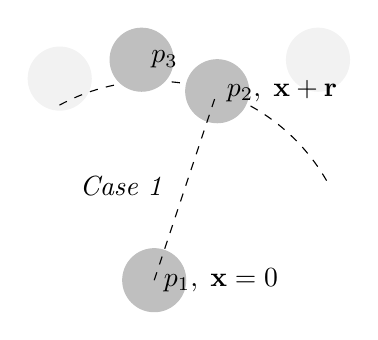
\begin{tikzpicture}[scale=0.8]
        \filldraw[ gray!10!white](+2.6,3.5)circle (0.5);
        \filldraw[ gray!10!white](-1.5,3.2)circle (0.5);
        \draw[dashed](30:3.16) arc (30:120:3.16);
        \filldraw[ gray!50!white](0,0) circle (0.5);
        \filldraw[ gray!50!white](1,3)circle (0.5);
        \filldraw[ gray!50!white](-0.2,3.5)circle (0.5);
        \draw(0,0)node[right]{$p_1, \; \textbf{x} = 0 $};
        \draw[dashed](0,0)--(1,3)node[right]{$p_2, \;\textbf{x}+\textbf{r}$};
        \draw[dashed](-0.2,3.5)node[right]{$p_3$};
        \node[ultra thick] (title) at (-0.5,1.5) {\textit{Case 1}};
    \end{tikzpicture} 
    \hfill
    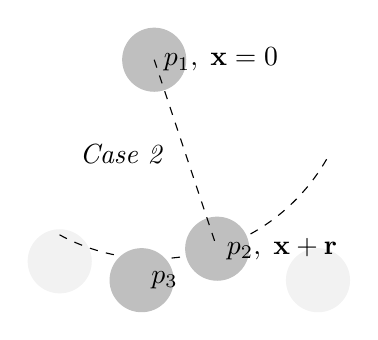
\begin{tikzpicture}[rotate=180, xscale=-0.8,yscale=0.8]
        \filldraw[ gray!10!white](+2.6,3.5)circle (0.5);
        \filldraw[ gray!10!white](-1.5,3.2)circle (0.5);
        \draw[dashed](30:3.16) arc (30:120:3.16);
        \filldraw[ gray!50!white](0,0) circle (0.5);
        \filldraw[ gray!50!white](1,3)circle (0.5);
        \filldraw[ gray!50!white](-0.2,3.5)circle (0.5);
        \draw(0,0)node[right]{$p_1, \; \textbf{x} = 0 $};
        \draw[dashed](0,0)--(1,3)node[right]{$p_2, \;\textbf{x}+\textbf{r}$};
        \draw[dashed](-0.2,3.5)node[right]{$p_3$};
        \node[ultra thick] (title) at (-0.5,1.5) {\textit{Case 2}};
    \end{tikzpicture} 
    \hfill
    % \begin{tikzpicture}[scale=0.8]
    %     \filldraw[ gray!10!white](+2.6,3.5)circle (0.5);
    %     \filldraw[ gray!10!white](-1.5,3.2)circle (0.5);
    %     \draw[dashed](-30:3.16) arc (-30:-120:3.16);
    %     \filldraw[ gray!50!white](0,0) circle (0.5);
    %     \filldraw[ gray!50!white](1,-3)circle (0.5);
    %     % \filldraw[ gray!20!white](-1.4,-3.3)circle (0.5);
    %     \filldraw[ gray!50!white](-0.2,-3.5)circle (0.5);
    %     % \draw[fill=gray,opacity=0.2](5,-0.2)circle (0.5);
    %     % \draw[fill=gray,opacity=0.2](-3,2)circle (0.5);
    %     % \draw[fill=gray,opacity=0.2](-5,0.2)circle (0.5);
    %     \draw(0,0)node[right]{$p_1, \; \textbf{x} = 0 $};
    %     \draw[dashed](0,0)--(1,-3)node[right]{$p_2, \;\textbf{x}+\textbf{r}$};
    %     \draw[dashed](-0.2,-3.5)node[right]{$p_3$};
    %     \node[ultra thick] (title) at (-0.5,-1.5) {$Case\; 2$};
    % \end{tikzpicture} 
    \caption{
        Diagram that highlights the asymmetry of the nearest pair statistic when the nearest neighbor is relatively far from the test particle.
        (\textit{Case 1}) Particle $p_1$ with  its nearest neighbor, $p_2$, located at the \underline{top} of it. 
        (\textit{Case 2}) Particle $p_1$ with  its nearest neighbor, $p_2$, located at the \underline{bottom} of it. 
        (\textit{Case 1} and \textit{2})
        In these situations the particle $p_2$ located at $\textbf{x} + \textbf{r}$, is the nearest neighbor of the particle $p_1$ located at $\textbf{x}$. 
        Since $|\textbf{r}|/d$ is assumed to be large, the nearest neighbor of the particle $p_2$ is more likely to be another nearest neighbor than $p_1$ such as the particle $p_3$, which is closer.
        This is due to the rapid decay of $P_\text{nst}$ for large $|\textbf{r}|/d$, see \ref{fig:Pnst_high_Ga}. 
        In these cases the nearest neighbor of $p_1$ is $p_2$, but the contrary is not true, inducing asymmetry in the statistics.  
    }
    \label{fig:diagram_asym}
\end{figure}

Now that this issue has been clarified, we can proceed to interpret the plots in \ref{fig:Why_Ga_matter}.
The beginning of the interactions happen at the early ages, meaning in the dark blue areas in  \ref{fig:Why_Ga_matter}, which are located on the top or bottom of the particle of reference.
The ending of the interactions corresponds to the greater ages, which are represented by the red areas. 
As shown by \ref{fig:Why_Ga_matter} (left), at low \textit{Galileo} number the nearest particle has a tendency to come from the top or bottom and leave through the sides. 
If the nearest particle is at a reasonable distance $|\textbf{r}| < 1.5d$ on the sides of the test particle, we can see that the vertical relative velocity is on average null, but positive in the radial component.
In this area, the age is at its maximum (dark red zone), therefore the interaction come to an end, meaning that the nearest particles get replace by another. 
Note that for the particles at a larger distance of the test particle, say $|\textbf{r}|>2$, have an averaged positive vertical relative velocity. 
As discussed above, in this situation the neighbor on the side is more likely to be closer to another particle. 
Consequently, if the test particle is isolated, with neighboring particles sufficiently far on the side, it will rise on average with a lower velocity than the latter particles.
Thus, particles at contact  seems to get apart because of the non-null radial velocity, and particle at distance seems to get apart because of the non-null vertical velocity.  
Consequently, on average the side-by-side configuration is not stable in this case, which partly explains why the particle distribution doesn't form any layer or such oriented microstructure at these $Ga$.   

% A plausible explanation for this phenomenon is that the leading particle accelerate the trailing particle with its wake on a first stage. 
% Then, the trailing particle arise to the same altitude as the leading particle, but still goes faster than the leading particle due to the acceleration provided by the wake of the latter particle.
% If the particles get in contact then the interaction duration seem to last longer, and the particles might even get trap in a small stagnation zone on the side of the particles.


For high \textit{Galileo} number, see \ref{fig:Why_Ga_matter} (right), the relative averaged velocity is nearly null on the sides and below the test particle. 
It is a statistical representation, meaning that, $\textbf{w}_p^r = 0$, just witnesses of the fact that the particles' relative velocity are not correlated with the relative position in this area. 
Thus, it is hard to say if the area where $\textbf{w}_p^r = 0$ corresponds to actual stagnation zones where both particles are in equilibrium, or if the relative velocity is just not correlated. 
Additionally, the particles at a large distance on the top of the test particle have a downward velocity. 
Meaning that if the test sphere is isolated and approach one or several  particles on the top of it (see \ref{fig:diagram_asym} (\textit{Case 1})), it will eventually catch up the latter particles. 
On the contrary, if the particle is isolated and that the nearest neighbor is at the bottom (see \ref{fig:diagram_asym} (\textit{Case 2})), the velocity is either pointing downward, or it is not correlated with the position, as indicated by the magnitude of $\textbf{w}_p^r$. 
A plausible explanation for this phenomenon is that the reference particle, when being isolated, goes faster than the potentially packed nearest neighbor.
Therefore, the test sphere can either catch up with the nearest particle if it is above, or move further away from it if it is below.
Also, it is interesting to notice that in this case the particles at near contact on the bottom of the test particles results from early interaction, denoted by the dark blue zone. 
It can be interpreted as follows : since 
initial time of interaction is on average low in this zone, it does mean that particles replace an old nearest neighbor that where at near contact of the test particles. 
Thus, in this case the nearest neighbor reaches the test sphere which were rising slowly because of a potentially close neighbor. 

Ultimately, the fields $\textbf{w}^r_p(\textbf{x},\textbf{r}, a)$ provide a quantitative averaged representation of what is known as the \textit{Drafting Kissing Tumbling} \citep{fortes1987nonlinear} mechanism. 
Indeed, in both case particles eventually approach from the verticals (\textit{Drafting}), nearly touch each other (\textit{Kissing}), and leave through the sides (\textit{Tumbling}). 
Statistically, the \textit{Tumbling} part is not present in the high inertial case, which  explains the creation of anisotropic structures or more stable side-by-side configurations. 
For bubble pair interactions \citet{zhang2021three} observed such DKT behavior.
They also reported side-by-side stable configuration of pairs. 
However, at same \textit{Galileo} than  \citet{zhang2021three} ($Ga = 10$) we were not able to identify this pair mechanism. 


To support the deduction made above, we displayed in \ref{fig:unst_ga} the absolute conditioned averaged center of mass velocity of the test sphere, defined as,
\begin{equation*}
    \textbf{u}^\text{r}_p(\textbf{x},\textbf{r},t)  
    =
    \frac{1}{P_r(\textbf{x},\textbf{r},t)}
    \int_0^\infty \textbf{u}^\text{nst}_pP_\text{nst}(\textbf{x},\textbf{r},t,a) da
\end{equation*}
In \ref{fig:unst_ga} (left) we clearly see that the magnitude of the test particle's vertical velocity is higher than the particle phase vertical velocity $\textbf{u}_p$ when the nearest neighbor is at near contact to the test particle, either above or below.
\begin{figure}[h!]
    \centering
    \includegraphics[height=0.35\textwidth]{image/HOMOGENEOUS_NEW/Dist/U_l_1_Ga_10_PHI_5.pdf}
    \includegraphics[height=0.35\textwidth]{image/HOMOGENEOUS_NEW/Dist/U_l_1_Ga_100_PHI_5.pdf}
    \caption{
         Quiver plots of the conditioned particle velocity field $\textbf{u}^\text{r}(\textbf{x},\textbf{r},t)$ colored by the averaged dimensionless vertical velocity difference : $(\textbf{u}^\text{r} - \textbf{u}_p )/ \textbf{u}_p$, for $\lambda = 1$ and $\phi = 0.05$. 
         (left) Low \textit{Galileo} number $Ga = 10$.
        (right) High \textit{Galileo} number $Ga = 100$.
         }
    \label{fig:unst_ga}
\end{figure}
When the nearest neighbor is at large distance of the test particle, its average velocity is lower than $\textbf{u}_p$. 
At high inertia however, the test particle velocity is higher when being isolated than with its neighbor at near contact. 
Additionally, we can see that when the particle is on the side at near contact or below, the test sphere's velocity  is lower than the mean. 
In brief in the case of $Ga = 10$ it seems that isolated particles goes slower than close neighbors packed together. 
While at higher \textit{Galileo} number it is the opposite, we observe that isolated particles  goes faster than packed neighbor. 


\subsubsection{The volume fraction dependency}
As it has been observed in \ref{fig:A} the effect of increasing $\phi$ is that it makes the particle distribution slightly more isotropic for $\phi >0.1$. 
\begin{figure}[h!]
    \centering
    \includegraphics[height=0.35\textwidth]{image/HOMOGENEOUS_NEW/Dist/U_rel_l_1_Ga_100_PHI_5.pdf}
    \includegraphics[height=0.35\textwidth]{image/HOMOGENEOUS_NEW/Dist/U_rel_l_1_Ga_100_PHI_20.pdf}
    % \includegraphics[height=0.35\textwidth]{image/HOMOGENEOUS_NEW/Dist/U_rel_l_10_Ga_100_PHI_10.pdf}
    % \includegraphics[height=0.35\textwidth]{image/HOMOGENEOUS_NEW/Dist/U_rel_l_1_Ga_100_PHI_10.pdf}
    \caption{Quiver plots of the relative averaged velocity field $\textbf{w}^\text{r}(\textbf{x},\textbf{r},t)$ colored by the averaged dimensionless age $a^r(\textbf{x},\textbf{r},t)$, for $Ga = 100$ and $\lambda = 1$. 
    (left) Low \textit{Galileo} number $\phi = 0.05$.
    (right) High \textit{Galileo} number $\phi = 0.2$. }
    \label{fig:Why_Phi_matter}
\end{figure}
In \ref{fig:Why_Phi_matter} we expose two situations with various volume fractions. 
In both graph we observe the same trend, despite the changes in length scales, which are due to the variations in volume fraction. 
Indeed, the stagnation zones with dark red color and the particle resulting from short interactions, dark blue color, are located approximately at the same location. 
We still observe the fore-aft asymmetry with respect to the horizontal plane, as it was discussed above. 
For other $\lambda$ and $Ga$ no particular differences could be observed with varying $\phi$. 
Overall, even if small differences might be present, the change in volume fraction doesn't seem to affect the relative kinematic of interaction between particles. 

\subsubsection{Influence of the viscosity ratio}

Lastly, we turn our attention to the effect of the viscosity ratio on pair relative kinematic.
The question that we are trying to answer is : why does a smaller viscosity ratio increase the anisotropy of the tensor $\textbf{R}(\textbf{x},t)$ as it is shown in \ref{fig:A}. 
With this objective in mind, we compare two cases at $Ga = 100$ and $\phi =0.05$, where we observe a clear difference between the distributions (see \ref{fig:Pnst_high_Ga}) between $\lambda = 1$ and $\lambda = 10$.
\begin{figure}[h!]
    \centering
    \includegraphics[height=0.35\textwidth]{image/HOMOGENEOUS_NEW/Dist/U_rel_l_10_Ga_100_PHI_5.pdf}
    \includegraphics[height=0.35\textwidth]{image/HOMOGENEOUS_NEW/Dist/U_rel_l_1_Ga_100_PHI_5.pdf}
    % \includegraphics[height=0.35\textwidth]{image/HOMOGENEOUS_NEW/Dist/U_rel_l_1_Ga_100_PHI_1.pdf}
    % \includegraphics[height=0.35\textwidth]{image/HOMOGENEOUS_NEW/Dist/U_rel_l_10_Ga_100_PHI_1.pdf}
    \caption{Quiver plots of the relative averaged velocity field $\textbf{w}^\text{r}(\textbf{x},\textbf{r},t)$ colored by the averaged dimensionless age $a^r(\textbf{x},\textbf{r},t)$, for $\phi = 0.05$ and $Ga = 100$. 
    (left) High viscosity ratio $\lambda = 10$.
    (right) Low viscosity ratio, $\lambda = 1$. }
    \label{fig:Why_l_matter}
\end{figure}
As in the previous cases, it is clear that for both cases in \ref{fig:Why_l_matter} the neighboring particle approach on the vertical direction and end up its course on the sides.
As discussed previously, the case on \ref{fig:Why_l_matter} (right) exhibit a clear stagnation zone and asymmetry on a vertical plane. 
On the other hand for $\lambda =10$ the relative velocity on the vicinity of the particle seem to be on average positive in the radial direction. 
In addition, The asymmetry aforementioned is not present in this case. 
As discussed in the previous paragraph, and explained by \ref{fig:diagram_asym}, the presence of the skew asymmetry in the fields $\textbf{w}_p^\text{r}$ about horizontal plane, witnesses for interactions of the isolated particles clusters of particles.
The absence of such asymmetry implies the absence of such interactions, indicating that the particles are more evenly spread. 

As before, it is interesting to investigate the value of the conditional velocity $\textbf{u}^r_p$ to better understand the particles collective interactions. 
Thus, \ref{fig:unst_l} display the fields  $\textbf{u}_p^\text{r}$ for both cases. 
\begin{figure}[h!]
    \centering
    \includegraphics[height=0.35\textwidth]{image/HOMOGENEOUS_NEW/Dist/U_l_10_Ga_100_PHI_5.pdf}
    \includegraphics[height=0.35\textwidth]{image/HOMOGENEOUS_NEW/Dist/U_l_1_Ga_100_PHI_5.pdf}
    \caption{
         Quiver plots of the conditioned particle velocity field $\textbf{u}^\text{r}(\textbf{x},\textbf{r},t)$ colored by the averaged dimensionless vertical velocity difference : $(\textbf{u}^\text{r}_p - \textbf{u}_p )/ \textbf{u}_p$, for $\phi = 0.05$ and $Ga = 100$. 
         (left) High viscosity ratio $\lambda = 10$.
         (right) Low viscosity ratio, $\lambda = 1$.
         }
    \label{fig:unst_l}
\end{figure}
On \ref{fig:unst_l} (left) we first notice that $\textbf{u}^\text{r}(\textbf{x},\textbf{r},t)$ behave similarly as the low inertial case display on \ref{fig:unst_ga} (left).
However, for $\lambda = 10$, the isolated particles' velocity is roughly equal to $\textbf{u}_p$. 
If isolated particle rise at the average velocity it is because the isolated particles constitute the majority of the realization since the trace of \textbf{R} is rather high, see \ref{fig:A}.
Therefore, this fact is not particularly relevant as it is just a statistical bias. 
Nevertheless, we can still conclude that for $\lambda = 10$ particles goes faster with a nearest neighbor on top or bottom, while for  $\lambda = 1$ particles goes faster when the nearest neighbor is at large distance. 

\subsubsection{Relation with the particle phase velocity fluctuation tensor}

In addition to provides physical explanation the field $\textbf{u}_p^d = \textbf{u}^r_p - \textbf{u}_p$ is of great importance to study the particle phase fluctuation tensor $\avg{\delta_i \textbf{u}_i' \textbf{u}_i'}$ which is of crucial importance in multiphase flow modeling. 
Indeed, it can be shown that 
\begin{equation*}
    \frac{\avg{\delta_i \textbf{u}_i' \textbf{u}_i'}}{n_p}(\textbf{x},t)
    =  
    \int_{\mathbb{R}^3 }
    \textbf{u}_p^d
    \textbf{u}_p^d
    P_{nst}(\textbf{r}|\textbf{x},t)
    d\textbf{r}
    + \int_{\mathbb{R}^3 }
    \textbf{F}(\textbf{r},\textbf{x},t)
    d\textbf{r}
\end{equation*}
where, $\textbf{F} = \avg{\sum_i\sum_{j\neq i}\delta_j\delta_i h_{ij}(\textbf{u}_i - \textbf{u}_p^{nst})(\textbf{u}_i - \textbf{u}_p^{nst})}$. 
Thus, the ensemble averaged particle phase Reynolds stress is the sum of the fluctuation given by $\textbf{u}_p^r$ plus an additional contribution form the others particles fluctuation around the average field $\textbf{u}_p^d$. 
At $\mathcal{O}(\phi)$ so the former term represents the majority of the particle phase fluctuation. 
Therefore, \ref{fig:unst_l} constitute a visual representation of the particle phase agitation tensor $\avg{\delta_i \textbf{u}_i' \textbf{u}_i'}$. 
Particularly, it can be seen on \ref{fig:unst_l}  that the particle phase fluctuations tensor is seen to be anisotropic. 
Indeed, more vertical velocity fluctuation than horizontal one is observed. 

\subsubsection{Discussion}
% \tb{
%     The field $\textbf{w}_p^r$ is useful for several reasons. 
%     As discussed it might serve to close equations such as \ref{eq:dt_R}. 
%     Or simply it provides us with clear physical explanation of what particles interaction look like. 
%     Also, we believe that it might be useful for coalesce kernels modeling. 

    
% }

From \ref{sec:Theory} we demonstrated that $\textbf{R}(\textbf{x},t)$ follows a transport equation were the tensor $\textbf{W}(\textbf{x},t)$ act as a source term. 
This tensor might be expressed as the symmetric part of $\int_0^\infty \textbf{r} \textbf{w}_p^\text{r} P(\textbf{x},\textbf{r},t) da$. 
Thus, the trends of the $\textbf{w}_p^\text{r}(\textbf{x},\textbf{r},t) $ in terms of the position determine the value of $\textbf{W}(\textbf{x},t)$ and partly determine the final value of $\textbf{R}(\textbf{x},t)$. 
In most of the graphs we observed that the vertical components of $\textbf{w}_p^\text{r}$ where negative when the vertical component of where positive \textbf{r} and vice versa. 
Consequently, $W_{yy}$ must be on average negative and $W_{xx}$ positive, which ultimately contribute to the value of $\textbf{R}(\textbf{x},t)$ and $\textbf{A}(\textbf{x},t)$ through \ref{eq:dt_R} and justify the sign of $A_{xx}$ in \ref{fig:A}. 

In \ref{fig:phase} we display the values of $W_{xx}$ in terms of $Ga$ and $\phi$. 
These graphs provide us with a concise description of the relative kinematic. 
We recall that $\textbf{W}:\bm\delta = 0$ as we demonstrated in \ref{sec:Theory}, thus the value  $W_{xx}$ entirely determine  $W_{yy}$ since the problem is symmetric. 
For example, we see that the highest dimensionless relative velocity position is reached for $Ga = 10$ and $\phi = 0.01$. 
This implies that it is in the dilute regime and with relatively small inertial effect that the particles have the fastest relative motions. 
\begin{figure}[h!]
    \centering
    \begin{tikzpicture}[scale=0.8]
        \node (img) at (0,0) {\includegraphics[height=5.5cm]{image/HOMOGENEOUS_NEW/PA/phase_Wxx_l_1.pdf}};
        \node (img) at (11,0) {\includegraphics[height=5.5cm]{image/HOMOGENEOUS_NEW/PA/phase_Wxx_l_10.pdf}};
    \end{tikzpicture}
    \caption{Phase diagram of the horizontal components of the dimensionless correlation tensor $W_{xx}/(Ud)$. 
        (left) Iso-viscous emulsion $\lambda = 1$.
        (right) Viscous droplets $\lambda = 10$ }
    \label{fig:phase}
\end{figure}
Is the relative velocity fields $\textbf{w}_p^r$ the cause of the microstructure's shape as it is suggested by \ref{eq:dt_R}. 
Or does $\textbf{w}_p^r$ is the consequence of microstructure shape, as it could be through looking at the previous graphs ?
Indeed, on \ref{fig:Why_l_matter} (right), the clear asymmetry with respect to the horizontal plane can be explained as the consequence of cluster  in the flows. 
Although it is tedious question, we believe that both are true, even if physical parameters also impact $\textbf{w}_p^r$, which makes the microstructure case dependent.  
Nevertheless, this makes $\textbf{W}(\textbf{x},t)$ potentially a function of $\textbf{R}(\textbf{x},t)$.
Depending on its relationship with $\textbf{R}(\textbf{x},t)$ this might modify the relaxation time.  
Thus, a more efficient way to close \textbf{W} by an objective manner would be to study the dynamic of interactions. 
In this work we only provided a kinematics arguments to explain the microstructure shape. 
Of course to fully understand the physics one has to study the dynamic of interaction. 
It is in fact possible in our framework to include such dynamic variable by deriving an equation for \textbf{W} the same way we derived \ref{eq:dt_R} for \textbf{R}.
% In this case it is reasonable to believe that the closure terms for the dynamical equation might be computable theoretically in terms of the physical parameters $Ga$, $\phi$ and $\lambda$. 




% \subsection{Carrier phase velocity fields}

In the previous section we explained the microstructure formation with kinematic arguments.
Although we indeed provided an explanation the question that arise now id :
Why does the relative velocity behave as such.
The answer might be obtained based on dynamical arguments as it is done often, in such a way we could explain the relative kinematic.
Nevertheless, the dynamical aspect of the interaction is out of the scope of this study and will be treated in a future work. 

Instead, we propose to study the particles averaged wakes to explain the possible difference in interaction between the iso-viscous and viscous droplets cases. 
Again we make use of the nearest particle averaged statistic to compute the carrier fluid phase velocity conditionally on the presence of a particle at \textbf{x}, it reads,
\begin{equation*}
    \textbf{u}^\text{nst}_f P_{nst}(\textbf{x},\textbf{r},t)= 
    \int \sum_{i}^{N_b} \delta(\textbf{x}-\textbf{x}_i(\FF,t))
    h_{i} 
    \textbf{u}_f^0(\textbf{x}+\textbf{r},t,\FF)
    d\mathscr{P} 
\end{equation*}
where $h_{i} = 1$ if the particle $i$ center of mass is the nearest point to the eularian coordinate \textbf{x}+\textbf{r}. 
This velocity fields can be reconstructed as well with our DNS. 
On \ref{fig:stream} we display the reconstructed velocity field $\textbf{u}^\text{nst}_f$ for (left) the iso-viscous case $\lambda =1$ and (right) the viscous droplets' case $\lambda = 10$, for different value of the volume fraction. 
\begin{figure}[h!]
    \centering
    \includegraphics[height=0.4\textwidth]{image/HOMOGENEOUS_NEW/Stream/Stream_PHI_1_Ga_100_l_100}
    \includegraphics[height=0.4\textwidth]{image/HOMOGENEOUS_NEW/Stream/Stream_PHI_1_Ga_100_l_10}
    \includegraphics[height=0.4\textwidth]{image/HOMOGENEOUS_NEW/Stream/Stream_PHI_5_Ga_5_l_100}
    \includegraphics[height=0.4\textwidth]{image/HOMOGENEOUS_NEW/Stream/Stream_PHI_5_Ga_5_l_10}
    \includegraphics[height=0.4\textwidth]{image/HOMOGENEOUS_NEW/Stream/Stream_PHI_20_Ga_100_l_100}
    \includegraphics[height=0.4\textwidth]{image/HOMOGENEOUS_NEW/Stream/Stream_PHI_20_Ga_100_l_10}
    % \includegraphics{image/HOMOGENEOUS_NEW/Stream/Stream_PHI_5_Ga_100_l_1.pdf}
    \caption{Nearest averaged carrier phase velocity fields. }
    \label{fig:stream}
\end{figure}
This velocity field is evaluated at $\textbf{x}+\textbf{r}$ conditioned on the presence of the nearest particle at $\textbf{x}$. 


\tb{compare with \citet{shajahan2023inertial} for explaination }

\section{Conclusion}
\section{Conclusion}

% \citet{einstein1905neue,taylor1932viscosity} demonstrated how the first moment of the hydrodynamic forces (Stresslet) applied on a particle immersed in pure linear flow induced an additional viscosity to the mixture. 
% Later~\citet{zhang1994ensemble,lhuillier1996contribution,jackson1997locally,zhang1997momentum} demonstrated that the second moment of forces were also contributing to the stresses inducing a non-newtonian behaviors, even in the Stokes and dilute limit.  

In this work we computed the moments of force on the surface of a test droplet in the situation of uniform relative motions between the droplet and the continuous phase. 
We considered low but finite Reynolds number $Re$. 
The averaged first moment of force is given by~\ref{eq:forces_reformulated2_avg}, scales as $O(\rho_f \phi u_r^2)$, hence contributing to the averaged Stress of the suspension on the same ground as  \citet{einstein1905neue} or \citep{taylor1932viscosity} correction to the viscosity of the mixture. 
In a lesser extend the inertial part of the second moment also contribute to the Rheology. 
This first point constitutes the main result of the paper. 

Others important conclusion reached through this work includes: a general reciprocal formula to derive the forces and moments on droplets, and the explicit appearing of the velocity variance term in the drag force term. 








\chapter{Closure modeling}
\label{chap:mono-disperse}
\localtableofcontents


\section{Average drag force}

\section{Average drag force}

%Objectives : 
%\begin{itemize}
%    \item Present the rising velocity Vs. phi to demonstrate the relation with $\phi^{1/3}$ \citep{loisy2017buoyancy}
%    \item Discus the common points and differences with bubbles and solid particles. 
%    \item Present a proper definition of the drag force terms such as in \citet{wang2021numerical}. 
%    \item Discus the possible correlation between the shape /arrangement of the particles/flow lines with the rising velocity. \tb{Je ne sais pas trop quoi dire la dessus}
%    \item Show that \citet{rusche2000effect}'s fit for the drag force is not adapted for our case and propose a new one
%    \item All the references for teh Drag force terms are in \citet[chap 8]{morel2015mathematical} or in \citet{ishii2010thermo}
%\end{itemize}
%\todo[inline]{include fits of bubbly flow}


%\JL{bien expliquer que ce que l'on mesure c'est les vitesses donc si on veut faire un modèle il faut repartir des vitesses (leur difference plus specifiquement). la pseudo turbulence entre elle dans la pression ou dans la viscosité ?}



%\begin{equation}
% F = ...
%\end{equation}
%On peut aussi parler du gradient de pression.


%The main difficulty is to relate the force to the flow parameters relative velocity between the two phases. 


In this section, we start by reviewing the various existing models for the averaged drag force acting on fluid inclusions in the Stokes regime. Subsequently, we consider the intermediate Reynolds number regime, the primary focus of our current investigation, proposing a drag model that reasonably fits the numerical results. As demonstrated in \ref{app:shape}, the droplet maintains an approximate spherical shape within the range of parameters studied here. Although slight deviations from sphericity are noted for $Bo=1$ and in configurations with the highest inertia, the maximum deviation from the spherical shape remains moderate less than $12$ \%. Hence, in this section we assume that fluid inclusions are spherical.

%. Henceforth, for the entirety of this section, we adopt the assumption that fluid inclusions exhibit spherical characteristics.

%Then we consider the intermediate Reynolds number regime studies which is the focus of the present work and propose a drag model which reasonably fits the numerical results. As demonstrated in Appendix \ref{app:shape} the droplet remains approximatively spherical within the range of parameters studied presently. Although some deviation from sphericity are observed for $Bo=1$ and in the highest inertial configurations the maximum deviation from the spherical shape remains moderate at around $10$ \%. Thus within the whole section, we will assume that the fluid inclusions are spherical. 


%In this section, we commence by examining existing models that describe the averaged drag force acting on fluid inclusions in the Stokes regime. Subsequently, we delve into the intermediate Reynolds number regime, the primary focus of our current investigation, proposing a drag model that effectively aligns with numerical results. As elucidated in Appendix \ref{app:shape}, the droplet maintains an approximate spherical shape within the studied parameter range. Although slight deviations from sphericity are noted for $Bo=1$ and in configurations with the highest inertia, the maximum departure from spherical shape remains modest at approximately 10%. Henceforth, for the entirety of this section, we adopt the assumption that fluid inclusions exhibit spherical characteristics.
  
%This assumption remains valid for the whole range of parameters investigated

\subsection{ The momentum balance in homogeneous sedimentation}

In the first place we would like to clarify several points about force balance and what it implies. 


\paragraph{Relation between forces and buoyancy :} The momentum conservation equations in the restricted situation of homogeneous sedimentation of particles reads from \ref{eq:dt_uc} and \ref{eq:dy_up} :
\begin{align}
    % \pddt (\phi_f\rho_f \textbf{u}_f)
    % + \div \left(\phi_f\rho_f \textbf{u}_f\textbf{u}_f + \phi_f  \bm{\sigma}_f^{\text{Re}} - n_p\textbf{M}_p \right)
    0 
    &= \phi_f 
    \left(\div \bm{\sigma}_f
    + \rho_f \textbf{g}\right)
    - n_p \textbf{f}_p, 
    \label{eq:dt_uf_steady}
    \\
    % \pddt (\phi_d\rho_d \textbf{u}_p)
    % + \div \left(\phi_d\rho_d \textbf{u}_p\textbf{u}_p+ \phi_d \bm{\sigma}_p^{\text{Re}}\right)
    0
    &= 
    \phi_d \left(\div \bm{\sigma}_f
    + \rho_d \textbf{g}\right)
    + n_p \textbf{f}_p. 
    % \label{eq:dy_up}
    \label{eq:dt_up_steady}
\end{align}
multiplying \ref{eq:dt_uf_steady} by $\phi_d$ and \ref{eq:dt_up_steady} by $\phi_f$ and subtracting the resulting equations gives, 
\begin{align}
    n_p \textbf{f}_p
    &= 
    \phi_d \phi_f (\rho_f -\rho_d ) \textbf{g}
    % \label{eq:dy_up}
\end{align}
In  mono-disperse suspension of droplets $n_p = \phi_d / v_p$ with $v_p =4/3\pi d^3/8$ the volume of a particle which yields the final results, 
\begin{equation*}
    \textbf{f}_p
    = 
    \frac{4}{3}\pi\frac{d^3}{8}\phi_f (\rho_f -\rho_d ) \textbf{g}
    \label{eq:drag}
\end{equation*}
It is convinient to make dimensionless this force with Hadamard-Ribczynski formula, which is, 
\begin{equation*}
    \textbf{f}^0_p = \pi \mu_f d A \textbf{u}_{pf}
\end{equation*}
Dividing one by the other gives the dimensionless force
\begin{equation*}
    \textbf{f}^*_p 
    = 
    \frac{4}{3A}\frac{d^2 \phi_f (\rho_f -\rho_d ) \textbf{g}}{8 u_{pf}\mu_f}
\end{equation*}
This can be made dimensionless with $\phi_f$



\paragraph{Relation between buoyancy and drag coefficient :}
We assume that the force can be written in the form, 
\begin{equation*}
    \textbf{f}_p = C_d  \pi \rho_f \frac{d^2}{8} u_{pf}^2
\end{equation*}
where $C_d$ is a dimensionless coefficient and $\textbf{u}_{fp}$ is the relative phase velocity. 
Using \ref{eq:drag} we show that $C_d$ coefficient is related to the relative velocity with, 
\begin{equation*}
    C_d  
    = 
    \frac{4}{3}
    \frac{d \phi_f (\rho_f -\rho_d ) \textbf{g}}{\rho_f u_{pf}^2}
\end{equation*}
This can be directly computed into our DNS. 
\begin{equation*}
    C_d  \phi_f^2 \frac{\rho_f^2 d^2 u_{pf}^2}{\mu_f^2}
    = 
    \frac{4}{3}
    \phi_f^3 
    \frac{
        d^3
        \rho_f
        (\rho_f -\rho_d ) g
    }{\mu_f^2}
\end{equation*}
Let us define the Galileo number as $Ga^2 = \frac{
    d^3
    \rho_f
    (\rho_f -\rho_d ) g
}{\mu_f^2}$ and the Reynolds number based on the drift velocity as, $Re =  \phi_f \frac{\rho_f d u_{pf}}{\mu_f}$,
Then, the relation between the Reynolds and Galileo is given by, 
\begin{equation*}
    Re
    = 
    Ga
    \sqrt{\frac{4\phi_f^3}{3 C_d}}
\end{equation*}
This the relative velocity is given by, 



In stokes and dilute regime the $C_d$ noted $D_c^0$ is given by Hadamard-Ribczynski solution and reads, 
\begin{equation*}
    C_d^0 = \frac{8}{Re} \left(\frac{3\lambda +2 }{\lambda +1}\right)
    = \frac{8}{Re}A
\end{equation*}
where we introduced the constant $A = \left(\frac{3\lambda +2 }{\lambda +1}\right)$. 
Thus, the Reynolds number obtained for a given \textit{Galileo} number in stokes regime is, 
\begin{equation*}
    Re^0
    = 
    \frac{Ga^2}{6 A}
    % \phi_f^3  
\end{equation*}
Since this is valid for an isolated particle we fixed $\phi_f=1$, this will be our renormalization constant. 
\begin{equation*}
    Re^*
    = 
    \frac{6A}{Ga}
    \sqrt{\frac{4\phi_f^3}{3 C_d}}
\end{equation*}
 
\paragraph{Relation between Galileo and Reynolds numbers :}
From the two previous expressions we can write the equality, 
\begin{equation*}
    \textbf{f}_p = C_d  \pi \rho_f \frac{d^2}{8} u_{pf}^2
\end{equation*} 
The hadamar ribinsky formula reads, 
\begin{equation*}
    \textbf{f}_p^0 =\pi \mu_f d A \textbf{u}_{pf}
\end{equation*}
dividing one by the other and by $\phi_f^2$ gives directly, 
\begin{equation*}
    \textbf{f}_p^* =   \frac{C_d  Re}{8 A \phi_f} 
\end{equation*}

\paragraph{Relation between dimensionless force and drag coefficient}

The hadamar-


\subsection{Stokes flow regime}

%From an experimental point of view it appears to be very challenging at most to measure the force acting on rising fluid particles in moderately dense regimes and relate it to the kinematic properties of the fluid and the particles. However, one may easily measure the mean settling or rising velocity of a suspension by measuring the velocity of its front \citep{guazzelli2011}. The mean velocity of fluid particles settling or rising in a finite vessel is known to be hindered, \textit{i.e.} to decrease with respect to the velocity of the isolated particle. Indeed the presence of a fixed bottom in a container leads to a zero velocity for the entire suspension (fluid + solid). Hence as the drops move upward, the fluid must move downward to compensate for the motion of the inclusions. This results in a decrease in the rising speed of the drops. It is usual to write this hindered velocity as  

From an experimental standpoint, quantifying the force exerted on ascending fluid particles in moderately dense conditions and establishing its correlation with the kinematic properties of both the fluid and the particles poses considerable challenges. Nonetheless, a feasible alternative involves measuring the mean settling or rising velocity of a suspension by measuring the velocity of its front \citep{guazzelli2011}. In a confined vessel, the mean velocity of fluid particles undergoing settling or rising is known to be hindered; that is, it decreases in comparison to the velocity of an isolated particle. The presence of a fixed container bottom induces a zero velocity for the entire suspension (comprising both continuous and dispersed phases). Consequently, as the droplets ascend, the fluid must move downward to counterbalance the motion of the inclusions, resulting in a reduction of the rising speed of the droplets \citep{guazzelli2011}. This hindered velocity is usually expressed as

%This decrease arises due to the presence of a stationary bottom in the container, causing the entire suspension (comprising both continuous and dispersed phases) to have a zero velocity \citep{guazzelli2011}. Consequently, as the droplets ascend, there is a compensatory downward movement of the fluid to counterbalance the motion of the inclusions, resulting in a reduction in the ascent speed of the droplets. This hindered velocity is conventionally expressed as...

%From an experimental standpoint, quantifying the force acting on ascending fluid particles in moderately dense conditions and establishing its correlation with the kinematic characteristics of both the fluid and particles poses considerable challenges. However, a more accessible metric involves determining the mean settling or rising velocity of a suspension by observing the velocity of its leading edge \citep{guazzelli2011}. In a confined vessel, the mean velocity of fluid particles settling or rising is recognized to be impeded, signifying a decrease relative to the velocity of an isolated particle. The presence of a fixed container bottom induces a zero velocity for the entire suspension (comprising both fluid and solid components). Consequently, as the droplets ascend, the fluid must descend to counterbalance the motion of the inclusions, resulting in a reduction of the rising speed of the droplets. This hindered velocity is conventionally expressed as


\begin{equation}
\frac{u_d}{u_0} = f(\phi)
\end{equation}
where $u_0$ is the rising speed of an isolated fluid inclusion and $f$ is a decreasing function of $\phi$. For fluid inclusion, in the Stokes regime ($Re=0$) the drag force is given by the Hadamard-Ribczynski formula $ F = -3\pi \mu d u_d (2/3+\lambda)/(1+\lambda)$. %drag coeficient is given by the Hadamard-Ribczynski formula 
Balancing this force with the buoyancy force one obtained the settling velocity of  spherical droplet in the Stokes regime

%\begin{equation}
%C_D = \frac{8}{Re} \left( \frac{2+3\lambda}{1+\lambda} \right)
%\end{equation}


\begin{equation}
    u_0
    = (\rho_c - \rho_d)\frac{g d^2}{18\mu_c}\left(\frac{1+\lambda}{2/3 + \lambda}\right),
    \label{eq:u_o}
\end{equation}
Hence a bubble rises 3/2 faster than a very viscous drop (or a solid sphere) of the same radius and density, the liquid properties being the same in each case.

The functional form of $f$ is much more complicated to obtain since it depends on both the microstructure and on the viscosity ratios. Specifically, for a dilute structure array consisting of a periodic arrangement of spherical inclusions, $f(\phi) =(1 - (2/3+\lambda)/(1+\lambda))a\phi^{1/3})$ where $a$ is a constant with a weak dependence on the specific form of the array \citep{sangani1987}. The decrease slope in velocity depends on $\lambda$. Indeed, the coefficient multiplying $c^{1/3}$ for a bubble ($\lambda=0$) is 2/3 of that for a solid particle ($\lambda \to \infty$). This is to be expected since this estimation is derived from the method of reflection and the aforementioned observation regarding the relative velocities of bubbles and solid particles. In contrast for random free array the function $f$ can be expressed as  $f(\phi) = (1-b(\lambda)\phi)$ where $b$ is a function approaching the value $6.5$ for large $\lambda$ and $4.5$ for small $\lambda$ \citep{wacholder1973,haber1981}. Once again, the rate of decrease is lower for bubbles compared to solid particles. We may also observe that the decrease of velocity as function of $\phi$ is much more pronounced for a structured array of inclusions compared to a random array. Hence the decrease of speed depends on the assumption made regarding the microstructure of the suspension \citep{davis1985}. In particular, rising bubbles at moderate Reynolds numbers show horizontal alignment of bubble pairs \citep{bunner2002,yin2006} which may suggest the use of a law designed for ordered microstucture. Interestingy, \citet{loisy2017} observed a decrease of the suspension velocity in $\phi^{1/3}$ in similar regime of Reynolds number. 

%The determination of the functional form of fff presents a heightened level of complexity due to its dependence on both microstructural features and viscosity ratios. Specifically, for a dilute structure array consisting of a periodic arrangement of spherical inclusions, f(ϕ)f(\phi)f(ϕ) is defined as (1−(2/3+λ)/(1+λ))aϕ1/3)(1 - (2/3+\lambda)/(1+\lambda))a\phi^{1/3})(1−(2/3+λ)/(1+λ))aϕ1/3), where aaa represents a constant with a weak dependence on the specific form of the array, as detailed by Sangani et al. (1987) \citep{sangani1987}. It is noteworthy that the diminution of velocity is contingent upon the parameter λ\lambdaλ, with the coefficient multiplying ϕ1/3\phi^{1/3}ϕ1/3 for a bubble being 2/32/32/3 times that for a solid particle. This alignment is anticipated, given that this estimation is derived from reflection methods and the aforementioned observation regarding the relative velocities of bubbles and solid particles.

%Conversely, for a random free array, the function fff can be expressed as f(ϕ)=(1−b(λ)ϕ)f(\phi) = (1-b(\lambda)\phi)f(ϕ)=(1−b(λ)ϕ), where bbb is a function converging towards 6.56.56.5 for large λ\lambdaλ and 4.54.54.5 for small λ\lambdaλ \citep{wacholder1973,haber1981}. Once again, it is evident that the rate of decrease is more gradual for bubbles compared to solid particles. Additionally, the reduction in velocity as a function of ϕ\phiϕ is more pronounced for a structured array of inclusions compared to a random array. Consequently, the deceleration of speed is contingent upon the assumptions made regarding the microstructure of the suspension \citep{davis1985}. Specifically, the ascent of bubbles at moderate Reynolds numbers exhibits the horizontal alignment of bubble pairs \citep{bunner,Yin}, implying a ϕ1/3\phi^{1/3}ϕ1/3-dependent velocity reduction, as recently observed by Loisy.



%and as mentionned above the force on an isolated bubble is 2/3  

%the term multiplying

% while for a random free array (see for instance Saffman for a discussion). The question of the microstructure in a suspension of settling particle is still open (citer Davis ...)



The results presented above are limited to very dilute configurations ($\phi \lesssim 5 \%$). However, in practical applications and especially in liquid-liquid extraction the volumic fraction of the dispersed phase can be as high as $20\%$. To adress moderately dense regimes, the current engineering approach involves resorting to empirical correlations such as the one developed by Richardson and Zaki  \citep{richardson1954}
%The current engineering practice, to obtain results in moderately dense regimes is to rely on empirical correlation such as the one developed by Richardson and Zaki  
\begin{equation}
f(\phi) = (1-\phi)^n
\label{eq:Richardson} 
\end{equation}
For solid spherical particles \citet{brzinski2018} have shown using data from 15 different studies drawn from the literature that $n$ is well approximated by $n\approx 4.5$. This approximation holds from very dilute regimes to dense regimes. As demonstrated in dilute flow there is a priori reason for this coefficient to be applicable to arbitrary viscosity ratios. \citet{ishii1979drag} by compiling various experiments found in the literature proposed values of $n\approx 3$ for bubbles and $n \approx 4$ for droplets. Hence, as in dilute flows the hindrance of the rising velocity is more pronounced for very viscous drops than low viscosity ones. To address this effect, we suggest the following correlation%To take into account this effect we propose the following correlation 

%As in diltute flows, an increase in the particle voulme fraction will make hinder
%there is a priori no reason for this coefficient to be valid for arbitrary viscosity ratio. 

%In this work we propose the following coefficient %In the most dilute configuration Wacholder oberseved a decrease of .... 

\begin{equation}
n(\lambda) = 4.5\left(\frac{2/3+\lambda}{1+\lambda}\right)
\label{eq:n}
\end{equation} 
which matches well the expressions proposed by \citet{brzinski2018} and \citet{ishii1979drag} in the limit of high and low viscosity ratios, respectively. There exist very few numerical results to validate this prediction. \citet{mo1994} have considered the fall of 16 drops within a tri-periodic box, revealing a coefficient $n$ slightly larger than in Equation \ref{eq:n} (details omitted here). The exact cause of this discrepancy remains uncertain and could stem from the slow decrease of the velocity perturbation in the Stokes flow regime. Indeed, special treatment are essential in this regime to ensure that the numerical results are independent from the number of inclusions \citet{mo1994}.

%There are very few numerical results to validate this prediction. \citet{mo1994} have considered the fall of 16 drops in a tri-peridoci box and found a coefficient $n$ slightly larger than equation \ref{eq:n} (results not shown here). We do not know the exact reason of this discrepancy which may be due to the slow decrease of the velocity perturbucation in the Stokes flow regime which require special treatment in the Stokes flow regime to make sure that the results are independent on the number of inclusions. %trestament of periodic interactions %Even if for Stokes flow  
%Indeed even in very diulte regime the hindered settling velocity is a function of $\lambda$.
Our focus has been exclusively on the upward velocity of a droplet suspension. Can this information be related with the mean drag force experienced by the droplets? In the Stokes regime, the answer is affirmative. This is emphasized in the book of \citep{jackson2000}, and we draw a similar line of reasoning for ascending droplets. By eliminating the pressure gradient in the equations \ref{eq:uf_triperio} and \ref{eq:up_triperio}, we obtain the force acting on the droplets as

%Up to know we have focused our attention entirely on the rising velocity of a suspension of drop. Is this information may be related to the mean drag force acting on the drops ? the answer is yes in the Stokes regime. This is empahsized in the book of \citep{jackson} and we present here a similar reasoning for rising drops. Eliminating the pressure gradient in equations ... we obtain the total force on the drops 
%This is emphasized in the book of Jackson but we repeat here for the sake of completness. 
\begin{equation}
nf_p = \phi(1-\phi)(\rho_d -\rho _c)g
\label{eq:bdf}
\end{equation}
where $nf_p$ is the vertical component of $n\mathbf{f_p}$. Due to the linearity of the Stokes equation the force per unit of volume may be expressed as $nf_p = A (u_c -u_d)$ where $u_c$ and $u_d$ are the vertical component of $\mathbf{u_c}$ and $\mathbf{u_d}$ and $A$ is a function to be determined. Inserting this estimate in equation \ref{eq:bdf} we obtain 

\begin{equation}
A = \frac{\phi}{(1-\phi)^{n(\lambda)-2}} \frac{(\rho_c -\rho_d)g}{u_0} 
\end{equation}
where we use the condition that the total velocity within the suspension is zero, expressed as $u\epsilon + v\phi=0$ and equation \ref{eq:Richardson}. The expression for the average force per unit of volume reads %Making use of 


%Then assuming that the mean velocity of the suspension is zero (as obtained from mass conservation for a fixed container) we get

\begin{equation}
nf_p = \frac{24}{Re_s}\left(\frac{2/3+\lambda}{1+\lambda}\right)\frac{3}{4}\frac{\rho |u_c-u_d|(u_c-u_d)}{d}\frac{\phi}{(1-\phi)^{n-3}}
\end{equation}
where $Re_s = (1-\phi)\rho |u_c-u_d| D/\mu$ is the Reynolds number based on the superficial velocity $u_s=(1-\phi) |u_c-u_d|$. From the former expression one may easily write the mean force on the particles as

\begin{equation}
f_p (Re_s,\lambda,\phi) = C_D^0(Re_s,\lambda)h(\lambda,\phi)\frac{1}{8}\rho \pi d^2 |u_c-u_d|(u_c-u_d)
\label{eq:FCD}
\end{equation}
where $C_D^0(Re_s,\lambda)=\frac{24}{Re_s}\left(\frac{2/3+\lambda}{1+\lambda}\right)$ is the modified drag coefficient on an isolated particle and $h(\phi,\lambda) =\frac{1}{(1-\phi)^{n-3}}$. This formulation is particularly interesting as it separates the effect of the Reynolds number from that of the void fraction in the total drag coefficient defined as $C_D(Re_s,\lambda,\phi) = C_D^0(Re_s,\lambda)h(\lambda,\phi)$. 

%This formula is of particular interest since it allows to separate the effect of the Reynolds number from the effect of the void fraction.
%where $C_D$ is the drag coefficient which can be expressed as $C_D = C_D^0\frac{\phi}{(1-\phi)^{n-3}}$ a



%Thus, one need the terminal velocity for a single particle

%They observed an hindered decrease of the velocitys 





%...

\subsection{Intermediate number Reynolds regime}

%In the range of the Reynolds number of the present study ($1 \lessim Re \lessim$), we cannot presuppose the form of the drag force as a function of the Reynolds number. This is exemplified in Figure \ref{fig:Re_Ga}. In this figure, one may see that the Reynolds number based on the relative velocity lies between the viscous scaling $Ga^1$ and the inertial scaling $Ga^2$. However one may also note that increasing the volume fraction does not significantly modify the slope of the curve. 

Within the Reynolds number range investigated in this study ($1 \lesssim Re \lesssim 100$), it is not possible to predefine the functional form of the drag force on the Reynolds number. This is illustrated in Figure \ref{fig:Re_Ga}. The figure reveals that the Reynolds number, based on the relative velocity, falls within the bounds of viscous scaling $Ga^1$ and inertial scaling $Ga^2$. It is noteworthy that increasing the volume fraction does not significantly modify the Reynolds number slope but simply shifts the points to higher $Ga$. Hence as in the previous subsection one may expect that separating the influence of the void fraction from the influence of the Reynolds number may be appropriate. This is a common approach, as seen in the widely applied Wen and Yu correlation \citep{wen1966}, employed for calculating forces in fluidized beds and sedimenting fluidized particles. Hence we assume that the mean force can be expressed as equation \ref{FCD}.


% la tendance est la meme quelque soit la frction volumique. Cela tends à nous indqiuer qu'un modele base sur un Cd isole qui va bien devrait fonctionner. En pratique il y a d'uatres modles (par exemple celui d'Ergun), amis dans le cas present il n'est pas adapté. Pour deux bonnes raison: deja il s'agit d'une superposition lineaire des deux 
%regimes lineaire et quadratique. PAr ailleurs il est fait pr des lits fixes

 





%\subsection{Steady drag force on an isolated spherical drop}
%First of all we want to investigate the dependency of the drift velocity with the volume fraction $\phi$. 
%It is known from several studies on the litterature, especially in \citep[chapter 8]{morel2015mathematical} and \citet[chapter 12]{ishii2010thermo} the the viscosity model for various system can be written generally, as,
%\begin{equation*}
%    \frac{\mu_m}{\mu_c}
%    = \left(
%        1 - \frac{\phi}{\phi_\text{max}}
%    \right)^{-2.5 \phi_\text{max}\mu_\text{eq}}
%\end{equation*}  
%with, $\mu_\text{eq} = \frac{\mu_d + 0.4 \mu_c}{\mu_d+\mu_c}$ and $\phi_\text{max}$ being the volume fraction corresponding to the \textit{maximum packing}. 
%\JL{la viscosite d'une suspension n'a rien a voir avec sa vitesse de chute meme si cela semble etre un argument donne dans la litterature... j'ai enleve tout cela pr l'instant}

%In this part, we briefly review the various formulas used to calculate the drag force on a spherical droplet embedded in a steady uniform flow.  Theoretical predictions for the force on a spherical droplet embedded in a steady uniform flow are limited to the limit of very small and very high Reynolds numbers. We define the drag coefficient, denoted as $C_D$ by the equation $F = \pi / 8 C_D \rho U_0^2 d^2$, where $F$ is the force on the drop, $U_0$ is the imposed velocity. The drag coefficient is a function of the Reynolds number $Re = \rho U_0 d /\mu $ and of is the viscosity ratio$\lambda = \mu _d /\mu _c$. % is the  as $F = C_D$ 
%In the Stokes regime ($Re=0$)the drag coeficient is given by the Hadamard-Ribczynski formula


%In this section, we briefly survey the diverse formulas applied to calculate the drag force acting on a spherical droplet within a steady, uniform flow. As corroborated in Appendix \ref{app:shape}, the droplet maintains an approximate spherical shape, a validity sustained across the entire spectrum of investigated parameters, even in the high inertial regime. Theoretical predictions for the force acting on a spherical droplet in a steady uniform flow are confined to scenarios of extremely low and exceptionally high Reynolds numbers.

%We define the drag coefficient, denoted as $C_D$, by the equation F=π8CDρU02d2F = \frac{\pi}{8} C_D \rho U_0^2 d^2F=8π​CD​ρU02​d2, where FFF signifies the force on the droplet, and U0U_0U0​ is the imposed velocity. This coefficient varies with the Reynolds number Re=ρU0dμRe = \frac{\rho U_0 d}{\mu}Re=μρU0​d​ and the viscosity ratio λ=μdμc\lambda = \frac{\mu_d}{\mu_c}λ=μc​μd​​. In the Stokes regime, the drag coefficient adheres to the Hadamard-Ribczynski formula.

%In the Stokes flow regime, the drag coefficient defined as $F = $

%drag force on a spherical drop embedded in a steady uniform flow is given by the Hadamard-Ribczynski formula
%\JL{il faut choisir ton echelle caractersitique de longueur. Soit $a$ le rayon soit le diametre des particules.}
%\begin{equation}
%F_0 = -\pi \mu d U \frac{2+3\lambda}{1+\lambda}
%\end{equation}

%\begin{equation}
%C_D = \frac{8}{Re} \left( \frac{2+3\lambda}{1+\lambda} \right)
%\end{equation}
%\ref{fig:U} shows the drift velocity $U$ divided by the stokes rising velocity of a spherical droplet $U_\text{stokes}$ defined in our notation as \citep{kim2013microhydrodynamics}, 
%Balancing the drag force obtained using the previous formula with the buoyancy force one obtained the settling velocity in the Stokes regime
%\begin{equation}
%    U_0
%    = (\rho_c - \rho_d)\frac{g d^2}{6\mu_c}\left(\frac{1+\lambda}{2 + 3\lambda}\right),
%\end{equation}
%or in dimensionless form 
%\begin{equation}
%    Re_0
%    = \frac{Ar^2}{6}\left(\frac{1+\lambda}{2 + 3\lambda}\right).
%\end{equation}
%where $Re_0 = \rho_c U_0 d/\mu_c$ is the Reynolds number based on the terminal velocity.
%In the opposite regime of very high Reynolds numbers ($Re\gg 1$), the flow outside the droplet can be considered as potential except in an infinitely thin boundary layer developing on the bubble surface. \citet{harper1968} have shown that the drag coefficient on a spherical drop is given by 

%\begin{equation}
%C_D = \frac{48}{Re}\left(1 + \frac{3\lambda}{2}\right).
%\label{eq:harper}
%\end{equation}
%Equation \ref{eq:harper} is the leading order expression in the expansion performed by \citet{harper1968} in the limit $Re\gg 1$. This equation tends toward Levich formula for the drag on a clean bubble in the limit $\lambda \ll 1$. A detailed investigation perfomed by \citet{dandy1989} have shown that the oroginal formulation by \citet{harper1968} became accurate for $Re\geq 200$. 

%Equation \ref{eq:harper} is the leading order term in the expansion carried out by \citet{harper1968} under the condition $Re\gg 1$. For $\lambda \ll 1$ this equation tends towards the Levich formula describing the drag on an uncontaminated bubble. A comprehensive investigation by \citet{dandy1989} revealed that the initial formulation proposed by \citet{harper1968} becomes accurate when $Re\geq 200$.

%\begin{equation}
%f_p (Re_s,\lambda,\phi) = C_D^0(Re_s,\lambda)g(\lambda,\phi)\frac{1}{8}\rho \pi d^2 |u-v|(u-v)
%\end{equation}
%where $C_D^0$ is the drag coefficient on an isolated drop and $g$ a function whose functional form is unknown \textit{a priori}.
Unfortunately in contrast to the Stokes regime there is no theoretical formula for the drag force on an isolated droplet for arbitrary Reynolds number. One may use potential flow theory (except in an infinitely thin boundary layer developing on the bubble surface) to predict the drag force on an isolated droplet in the limit  $Re\gg 1$ \citep{harper1968}, but numerical computations have shown that the theory is only accurate for $Re\geq 200$ \citep{dandy1989}.
%The above review show that in the intermediate Reynolds number regimes of the present study $ 1 \lesssim Re \lesssim 100$, there is no theoretical formulas. 
Hence in practice one have to rely on empirical relationship to predict the drag force on the drop. \citet{rivkind1970} proposed to write a drag force as a combination of the drag force on a solid spherical particle
(the limit ($\lambda \rightarrow \infty$) and the drag force on a spherical bubble ($\lambda \rightarrow 0$)

\begin{equation}
C_D^0(Re,\lambda) = \frac{C_{Ds}^0(Re)+\lambda C_{Db}^0(Re)}{1+\lambda}
\label{eq:CD0}
\end{equation}
where $C_{Ds}^0$ is the drag force on an isolated solid sphere and $C_{Db}^0$ the drag force on a shear-free bubble. Formula \ref{eq:CD0} constitutes a generalization of the Hadamard-Ribczynski formula in the intermediate Reynolds number regime. As suggested by \citet{magnaudet1997} we make use of the following correlation for the drag force on a solid particle and a bubble
\begin{align}
C_{Ds} ^0 &= \frac{24}{Re}(1+0.15Re^{0.687}) \\
%\end{equation}
%\begin{equation}
C_{Db} ^0 &= \frac{16}{Re}\left(1+\left[\frac{8}{Re}+\frac{1}{2}\left(1+3.315Re^{-1/2}\right)\right]^{-1}\right)
\end{align}
which where originally proposed by \citet{schiller1933} and \citet{mei1994} respectively. Formula \ref{eq:CD0} agrees with numerical results with an error of $5-7\%$ \citep{rivkind1970}.%Balancing the drag force obtained using the previous formula with the buoyancy force one obtained the settling velocity

%\begin{equation}
%C_D(Re)Re^2=\frac{4}{3}Ga ^2
%\label{}
%\end{equation}


%where higher order terms can be found in the original publication of \citet{harper1968}. 

%to leading order as $Re = \rho U_0 d /\mu$ 


%In practice the above formula are very limited randge of validity and empirical formulation have to be used for intermediate Reynolds numbers. Prendre la correlation de Rykind et Ryskin


%\begin{equation}
%nf_p = C_D(Re_s)\frac{3}{4}\frac{\rho _c |u_c-u_d|(u_c-u_d)}{D}\frac{\phi}{(1-\phi)^{n-3}}
%\end{equation}


%with $C_D^0$ given by "Jacques" Formula and  $h(\lambda,\phi)=\frac{1}{(1-\phi)^{n-3}}$
%We will now assume that the functional form of $f(\phi)$ is the same as in the Stokes flow regime and is thus indendent of the Reynolds number. This assumption, has no theoretical ground but \citet{di1994} has shown that $f$ is weakly dependent of the Reynolds number for solid particles. 
We will assume that the functional expression of $f$ remains the same with that observed in the Stokes flow regime, thereby assuming that it is independent of the Reynolds number. While this assumption has no theoretical ground, \citet{di1994} demonstrated that the dependency of $f$ on the Reynolds number for solid particles is small especially for low solid volume fraction.





\subsection{Comparison with the numerical results}


We now present our results by comparing the sedimentation velocity predicted by \ref{eq:CD0} and the sedimentation measured from our DNS. 
The averaged velocity displayed in \ref{fig:drag_force} is made dimensionless using the terminal velocity of an isolated buoyant droplet in stoke flow \eqref{eq:u_o}. 
\begin{figure}[h!]
    \centering
    \includegraphics[height = 0.25\textwidth]{image/HOMOGENEOUS_final/CA/U_l_10.pdf}
    \includegraphics[height = 0.25\textwidth]{image/HOMOGENEOUS_final/CA/U_l_1.pdf}
    \includegraphics[height = 0.25\textwidth]{image/HOMOGENEOUS_final/CA/U_l_0.pdf}
    \caption{
        Dimensionless rising velocities for (top left) $\lambda  = 10$ (top right) $\lambda =1$ and (bottom) $\lambda = 0.1$. 
        The symbols represents the differents \textit{Galileo} numbers. 
        (dashed lines) Theoretical prediction form \ref{eq:CD0}. 
    }
    \label{fig:drag_force}
\end{figure}



%\subsection{Interphase drag force}
%\subsection{Droplets configurations flowlines and deformations }

\section{The Reynolds stress}

Objectives : 
\begin{itemize}
    \item Present the decomposition of the fluid reynolds stress according to isotropic and deviatoric part.
    \item Show the relation between the flowlines graphs and the actual values of the velocity fluctuation.
    \item Compare our case with \citet{almeras2019fluctuations}
\end{itemize}



We decompose both Reynolds stress into an isotropic part and deviatoric part such that, 
\begin{align}
    \bm{\sigma}^{\text{Re}}_p &=  \rho_d \phi_d K^*_p
    \left[
        \textbf{I}(\textbf{u}_p - \textbf{u}_c)\cdot (\textbf{u}_p - \textbf{u}_c) 
        +\textbf{B}_c \cdot (\textbf{u}_p - \textbf{u}_c)(\textbf{u}_p - \textbf{u}_c)
    \right]\\
    \bm{\sigma}^{\text{Re}}_c &=  \rho_c \phi_c K_c^*
    \left[
        \textbf{I}(\textbf{u}_p - \textbf{u}_c)\cdot (\textbf{u}_p - \textbf{u}_c) 
        +\textbf{B}_p \cdot (\textbf{u}_p - \textbf{u}_c)(\textbf{u}_p - \textbf{u}_c)
    \right]
\end{align}
where the $K^*$ is the dimensionless pseudo-turbulent  kinetic energy, $\textbf{I}$ a unit tensor and $\textbf{B}$ a tensor accounting for the deviation of the Reynolds stress left to determine. 

\subsection{The continuous phase Reynolds stress}
\todo{try \citet{almeras2021statistics} fits}
\todo{also check \citet{almeras2019fluctuations} results}
\tb{might be good to plot the velocity field to examine where does the fluctuation arise (pseudo-turbe or turbe)}
Look at \citep{wang2021numerical} and Mahra.. 2015 



The fluid averaged kinetic energy can be easily scaled on the numerical results shown \ref{fig:Tf_Bf}(left).
\begin{figure}[h!]
    \centering
    \includegraphics[height=0.3\textwidth]{image/HOMOGENEOUS/fCA/Tf_l_1.pdf}
    \includegraphics[height=0.3\textwidth]{image/HOMOGENEOUS/fCA/Bf_l_1.pdf}

    \includegraphics[height=0.3\textwidth]{image/HOMOGENEOUS/fCA/Tf_l_10.pdf}
    \includegraphics[height=0.3\textwidth]{image/HOMOGENEOUS/fCA/Bf_l_10.pdf}
    \caption{(left) Dimensionless turbulent kinetic energy in terms of the \textit{Galileo} number for different $\phi$. (dots) Numerical simulations, (dashed line) empirical formula \ref{eq:Tf_scaling}.
    The symbols correspond to different volume fraction ($\bullet$) $\phi = 1\%$, ($\blacktriangle$) $\phi = 5\%$, ($\blacksquare$) $\phi = 10\%$, ($\blacklozenge$) $\phi = 15\%$ and ($\blacktriangleright$) $\phi = 20\%$.
    (right) deviatoric part of the Reynolds stress, ($- \cdot -$)  vertical components, $B_{yy}$, ($- -$)  horizontal components, $B_{xx} = B_{zz}$.}
    \label{fig:Tf_Bf}
\end{figure}
\subsection{The particles phase Reynolds stress}

\tb{Maybe include velocity fluctuation and compare to : Lingxin2021 }

\tb{Include Gaussian distribution of bubbles !!! ! ! ! }
Now let's focus on the particular averaged Reynolds stress tensor.
\ref{fig:Talpha_Balpha} shows that the granular temperature behavior is quite similar from the continuous averaged turbulent kinetic energy.
\begin{figure}[h!]
    \centering
    \includegraphics[height=0.3\textwidth]{image/HOMOGENEOUS/fPA/Talpha_l_1.pdf}
    \includegraphics[height=0.3\textwidth]{image/HOMOGENEOUS/fPA/Balpha_l_1.pdf}

    \includegraphics[height=0.3\textwidth]{image/HOMOGENEOUS/fPA/Talpha_l_10.pdf}
    \includegraphics[height=0.3\textwidth]{image/HOMOGENEOUS/fPA/Balpha_l_10.pdf}
    \caption{(left) Dimensionless turbulent kinetic energy in terms of the \textit{Galileo} number for different $\phi$. (dots) Numerical simulations, (dashed line) empirical formula \ref{eq:Talpha_scaling}.
    (right) deviatoric part of the Reynolds stress, ($\bullet$) are the vertical components, $B_{yy}$, ($\blacktriangle$) are the horizontal components, $B_{xx} = B_{zz}$.}
    \label{fig:Talpha_Balpha}
\end{figure}
We can also provide a scaling for the granular temperature, it reads as,  
\begin{equation}
    \frac{\pnavg{T_\alpha}}{U^2}  \approx \frac{\phi}{Ga^2} 2.86\cdot10^{4} 
    \label{eq:Talpha_scaling}
\end{equation}
From \ref{fig:Talpha_Balpha} we observe that this scaling is valid for the lowest \textit{Galileo}. 
The deviatoric part of $\pnavg{T_\alpha}$ is displayed on \ref{fig:Talpha_Balpha}.
It tells us that the Reynolds stress for the particular phase tends to be isotropic in the same way as $\cavg{T}$. 
Indeed, the components of $\pnavg{\textbf{B}}$ go to zero with increasing $Ga$ and $\phi$. 
This behavior is explained by the higher rate of collision present for higher volume fraction and inertia \citep[chapter 1]{jackson2000dynamics}

% \chapter{Mono-disperse buoyant water/oil emulsion.}
\label{chap:mono-disperse}

In this chapter we present the results related to the mono-disperse buoyant rising  emulsion of droplets.
All the simulations files can be found here \url{http://basilisk.fr/sandbox/fintzin/Rising-Suspenion/}
This chapter will cover the different closure terms that we brought to light in \ref{chap:avg}, such as the mean slip velocities or drag force, the Reynolds stress tensor and the particle stress tensor.
Even through we forced non coalesce in these simulations we will still discuss the possibility to close the collision kernel of PBE or Lagrangian equations. 
Also in this chapter we will solely focus on the momentum equations closure, and neglect mass transfer terms. 
\begin{figure*}
    \centering
    \includegraphics[width = 0.8 \textwidth]{image/PHI_01_Ga_75.png}
    \caption{Snapshot of a simulation at $T_g = 300$ for $\phi = 0.1$, $Ga = 75$ $\mu_r = 0.1$ and $N_b = 125$. In white : the interfaces, The background color map correspond to the pressure field. The grid represents the different core.}
    \label{fig:pic_sim}
\end{figure*}
As a consequence of the mono-disperse assumption it is evident that the mass balance and number density balance are similar. 
However, the surface balance (\ref{eq:A_avg_p}) remains relevant as the surface of all particles is not constant since it is a function of the deformation. 
However, as it will be shown in the low \textit{Bond} numbers limit the droplets remain spherical allowing us o discard this equation too. 
Therefore, In this context we be interested in the momentum balance's (\ref{eq:classic_hybrid_momentum_p} and \ref{eq:classic_hybrid_momentum_c}) closures. 
Neglecting the mass transfer terms and considering the mass as a constant yields the following particular and continuous averaged momentum equations, 
\begin{multline}
    \rho_c\pddt (\phi_c\cavg{\textbf{u}}) 
    + \rho_c\nablab \cdot ( \phi_c \cavg{\textbf{u}}\cavg{\textbf{u}})
    = \pavg{\int_{S_\alpha} \textbf{T}_c  \cdot \textbf{n}_c d S}
    +\phi_c\cavg{\textbf{b}}\\
    + \nablab\cdot\left[
    \phi_c \cavg{\textbf{T}}
    - \pavg{\int_{S_\alpha} \textbf{r} \textbf{T}_c  \cdot \textbf{n}_c dS}
    - \rho \cavg{\textbf{u}'\textbf{u}'}
    \right],
    \label{eq:homo_momentum_c}
\end{multline}
\begin{multline}
    \pddt   \left(\pavg{\textbf{u}_\alpha}\right)
    + \nablab \cdot \left(\pavg{\textbf{u}_\alpha}\pnavg{\textbf{u}_\alpha}\right)
    = \frac{n}{m_\alpha}\pnavg{\int_{V_\alpha} \textbf{b} dV}\\
    + \frac{n}{m_\alpha}\pnavg{\int_{S_\alpha} \textbf{T}_c  \cdot \textbf{n}_c dS}
    - \nablab \cdot \left(\pavg{\textbf{u}_\alpha' \textbf{u}_\alpha'}\right). 
    \label{eq:homo_momentum_p}
\end{multline}
From these simplified equations we can start to complete the closure problem.

Since all simulations reach as quasi static regime we can stipulate that the averaged velocities vector are constants and vertical. 
Therefore, all along this chapter we note the drift velocity such as $U = \pnavg{\textbf{u}} - \cavg{\textbf{u}}$. 
Besides, in this chapter we fix the following dimensionless parameters to $\rho_r =1.11 $, $\mu_r =0.1$, $Bo =1$ and $N_b = 125$. 
As a consequence of the small \textit{Bond} number in presence, the droplets are nearly spherical. 
A picture of a typical simulation is shown \ref{fig:pic_sim}
% \section{The drag force term}
We start by the drag force term. 
Our simulations reach a quasi steady regime meaning that we can consider the velocities of the particular phase and fluid phase as constant.
Now lat's place our selves in the reference frame moving at the averaged velocity of the particles. 
In this frame of reference the particles are thus fixed and see the fluid flowing through, experiencing a drag force due to the stress on the droplets surface. 
Therefore, in this referential considering $\pavg{\textbf{u}} = \textbf{0}$, the momentum equation \ref{eq:homo_momentum_p} yields, 
\begin{equation*}
    m_\alpha \grad \cdot \left(\pavg{\textbf{u}_\alpha' \textbf{u}_\alpha'}\right). 
    = \pavg{\int_{V_\alpha} \textbf{b} dS}
    + \pavg{\int_{S_\alpha} \textbf{T}_c  \cdot \textbf{n}_c dS}
\end{equation*}
\tb{to be disscused}
We can observe that the divergence of the fluctuation is balanced by the two contributions to the RHS.  
Besides, the body force term has the simple expression, $\pavg{\int_{V_\alpha} \textbf{b} dV} = - nV_\alpha (\rho_d-\rho_c) \textbf{g}$. 
Therefore, the drag force term must be expressed as the sum of a pure drag force which balance the body force and a divergence of a stress which balance in this can the Reynolds stress \citep{zhang2021ensemble,wang2021numerical,nott2011suspension}. 
In this section we focus on the pure drag component and expresses it in the dimensionless form such as, 
\begin{align*}
    \pnavg{F_\mu}
    = \frac
    {\pnavg{\int_{V_\alpha} \textbf{T}\cdot \textbf{n}dV}}
    {\mu_c U D}
    = \frac
    {\left(\rho_d -\rho_c\right) \textbf{g}}
    {\mu_c U}D^2
\end{align*}
Where $\pnavg{F_\mu}$ is the pure dimensionless drag force along the direction of the velocity. 

\ref{fig:f_mu} displays the interphase drag force for different \textit{Galileo} number and volume fraction. 
\begin{figure}[h!]
    \centering
    \includegraphics[height=0.3\textwidth]{image/HOMOGENEOUS/fCA/FH_mu_Ga.pdf}
    \includegraphics[height=0.3\textwidth]{image/HOMOGENEOUS/fCA/UstokesGa.pdf}
    \caption{(left) Dimensionless drag forces in terms of the \textit{Galileo} number for different volume fraction $\phi$. The other parameters are fixed at $\rho_r = 1.11$, $\mu_r = 0.1$ and $Bo = 1$.
    (dots) Numerical simulations, 
    (dashed line) empirical formula \ref{eq:f_mu_scaling}.
    (right) Dimensionless drift velocity.}
    \label{fig:f_mu}
\end{figure}
Based on the numerical results we could find simple scaling for the drag force at moderate inertial regime. 
Indeed, it yields,
\begin{equation}
    \cavg{F^\mu} = e^{5.66 \phi^{1/3}}  Ga^{0.33} 0.59 + Ga^{0.92} +18.29
    \label{eq:f_mu_scaling}
\end{equation}
From \ref{fig:f_mu} and \ref{eq:f_mu_scaling} it is evident  that in low inertial regime, the drag force scales as $f \sim Ga^{0.33}$ regardless of the volume fraction. 
Regarding the dependency of the force with $\phi$, we observe that the logarithms of the force is proportional $\phi^{1/3}$. 
This reminds the scaling of \cite{sangani1987sedimentation} which found the same $\phi$'s dependency, but on the drift velocity of arranged bubbles arrays.
This scaling is illustrated \ref{fig:f_mu} (right) where we can see that the drift velocity is indeed proportional to $\phi^{1/3}$ regardless of the \textit{Galileo} number.  
% \section{Reynolds stress closure}
Now let's investigate the Reynolds stress sensor, for both the continuous and the particular phase.
We first decompose the stress tensor by a sum of a spherical and deviatoric part \citep[chapter 6]{morel2015mathematical}, such as, 
\begin{equation*}
    \cavg{\textbf{u'u'}}
    = \frac{2}{3}\cavg{T}\left(
        \textbf{I}
        + \cavg{\textbf{B}}
    \right),
\end{equation*}
where we introduced the turbulent kinetic energy, $\cavg{T} = \frac{1}{2}\cavg{\textbf{u'u'}}:\textbf{I}$ and the deviatoric part of the Reynolds stress as, 
$\cavg{\textbf{B}} = \cavg{\textbf{u'u'}}/(2\cavg{T}) - \frac{1}{3}$.
A similar logic can be applied to the particular averaged Reynolds stress yielding, 
$
\pnavg{\textbf{u}'_\alpha \textbf{u}_\alpha'}
    = \frac{2}{3}\pnavg{T_\alpha}\left(
        \textbf{I}
        + \pnavg{\textbf{B}_\alpha}
    \right)
$.
In this case $\pnavg{T_\alpha}$ is the granular temperature from kinetic theory \citep{rao2008introduction}. 
Note that the non-diagonal components of $\cavg{\textbf{B}}$ and  $\pnavg{\textbf{B}_\alpha}$ are all null due to the symmetry of the model. 
Therefore, they will not be shown here. 
\subsection{The continuous phase Reynolds stress}
The fluid averaged kinetic energy can be easily scaled on the numerical results shown \ref{fig:Tf_Bf}(left).
Indeed, we found out that 
\begin{equation}
    \frac{\cavg{T}}{U^2} \approx \frac{\phi}{Ga^2}5.98\cdot10^{4} ,
    \label{eq:Tf_scaling}
\end{equation}
where we use the drift velocity $U$ to make $T$ dimensionless. 
\begin{figure}[h!]
    \centering
    \includegraphics[height=0.3\textwidth]{image/HOMOGENEOUS/fCA/Tf.pdf}
    \includegraphics[height=0.3\textwidth]{image/HOMOGENEOUS/fCA/Bf.pdf}
    \caption{(left) Dimensionless turbulent kinetic energy in terms of the \textit{Galileo} number for different $\phi$. (dots) Numerical simulations, (dashed line) empirical formula \ref{eq:Tf_scaling}.
    (right) deviatoric part of the Reynolds stress, ($\bullet$) are the vertical components, $B_{yy}$, ($\blacktriangle$) are the horizontal components, $B_{xx} = B_{zz}$.}
    \label{fig:Tf_Bf}
\end{figure}
In opposition to the drift velocity, the dimensionless turbulent kinetic energy scale as $\sim \phi$ regardless of the \textit{Galileo} number. 
As shown previously $U \sim \phi^{1/3}$, consequently the turbulent kinetic energy scale as $\cavg{T} \sim \phi^{5/3}$. 
Besides, $\cavg{T}$ is a monotonic function of $Ga$ with a growth rate of $0.91$. 
Regarding the deviatoric part of the Reynolds stress tensor, namely, $\cavg{\textbf{B}}$, it can be approximated by, roughly, $\cavg{\textbf{B}_{yy}} \approx 0.4$ and $\cavg{\textbf{B}_{zz}} = \cavg{\textbf{B}_{xx}}  \approx - 0.2$.
Therefore, the \textit{Reynolds} stress is clearly oriented, indeed the stress is greater in the direction of the flow. 
Also, as depicted by \ref{fig:Tf_Bf} (right), at high $Ga$ and $\phi$ those components slightly tend to lower values, whether it is for the horizontal or vertical components. 
This means that the global Reynolds stress tends to be isotropic with for high $Ga$ and $\phi$. 
In \citet{jackson2000dynamics} they stipulate that at high rate of collision the \textit{Reynolds} stress tends to be isotropic. 
Which is in accordance with our findings since, $Ga$ and $\phi$ are directly correlated to the rate of collision. 
For now a good approximation of $\cavg{\textbf{B}}$ is 
\begin{equation}
    \cavg{\textbf{B}} 
    \approx 0.4 \textbf{dd} + 0.2 (\textbf{I} - \textbf{dd}),
    \label{eq:Bf_scaling}
\end{equation}
where $\textbf{d}$ is the unit vector following the direction of the flow, in our case, $\textbf{d} = \textbf{g}/g$ or more generally, $\textbf{d} = U/|U|$. 

\subsection{The particular phase Reynolds stress}
Now let's focus on the particular averaged Reynolds stress tensor.
\ref{fig:Talpha_Balpha} shows that the granular temperature behavior is quite similar from the continuous averaged turbulent kinetic energy.
\begin{figure}[h!]
    \centering
    \includegraphics[height=0.3\textwidth]{image/HOMOGENEOUS/fPA/Talpha.pdf}
    \includegraphics[height=0.3\textwidth]{image/HOMOGENEOUS/fPA/Bf.pdf}
    \caption{(left) Dimensionless turbulent kinetic energy in terms of the \textit{Galileo} number for different $\phi$. (dots) Numerical simulations, (dashed line) empirical formula \ref{eq:Talpha_scaling}.
    (right) deviatoric part of the Reynolds stress, ($\bullet$) are the vertical components, $B_{yy}$, ($\blacktriangle$) are the horizontal components, $B_{xx} = B_{zz}$.}
    \label{fig:Talpha_Balpha}
\end{figure}
We can also provide a scaling for the granular temperature, it reads as,  
\begin{equation}
    \frac{\pnavg{T_\alpha}}{U^2}  \approx \frac{\phi}{Ga^2} 2.86\cdot10^{4} 
    \label{eq:Talpha_scaling}
\end{equation}
From \ref{fig:Talpha_Balpha} we observe that this scaling is valid for the lowest \textit{Galileo}. 
The deviatoric part of $\pnavg{T_\alpha}$ is displayed on \ref{fig:Talpha_Balpha}.
It tells us that the Reynolds stress for the particular phase tends to be isotropic in the same way as $\cavg{T}$. 
Indeed, the components of $\pnavg{\textbf{B}}$ go to zero with increasing $Ga$ and $\phi$. 
This behavior is explained by the higher rate of collision present for higher volume fraction and inertia \citep[chapter 1]{jackson2000dynamics}
% \section{The first moment}
In this section we will be interested into the first moment tensor appearing in \ref{eq:homo_momentum_c}, namely the average of the tensor $\textbf{D}_\alpha = \int_{S_\alpha} \textbf{r}\textbf{T}_c\cdot \textbf{n}_c dS = \int_{S_\alpha} \textbf{rf}_c dS$, where we introduced the microscopic hydrodynamical force vector $\textbf{f}_c = \textbf{T}_c\cdot \textbf{n}_c$.
Following the same approach as the analysis of \citet[chapter 2]{kim2013microhydrodynamics} we decompose the first moment tensor into two distinct tensors and remove the isotropic part of $\textbf{D}_\alpha$, yieldings
\begin{equation*}
    \textbf{D}_\alpha - \frac{1}{3}(\textbf{I}:\textbf{D}_\alpha)\textbf{I}
    = \textbf{S}_\alpha+\textbf{T}_\alpha,
\end{equation*}
where $\textbf{S}_\alpha$ is the stresslet tensor and $\textbf{T}_\alpha$ the hydrodynamical torque acting on the particle. 
Besides, because of numerical limitations, we prefer to use the force defined inside the dispersed phase $\textbf{f}_d$ instead of original force, $\textbf{f}_c$. 
It is possible to switch from a force to another by making use of the jumps condition (\ref{eq:stressjump}) defined in \ref{chap:avg}, i.e. $\textbf{f}_c = \textbf{f}_I - \textbf{f}_d$. 
Consequently, we can write that $\textbf{D}_\alpha = \textbf{D}_\alpha^I + \textbf{D}_\alpha^h$, where $\textbf{D}_\alpha^h$ is the hydrodynamical contribution to the first moment and $\textbf{D}_\alpha^I$ the surface tension force contribution. 
Applying the same decomposition for the torque and stresslet tensors yields,
\begin{align*}
    \textbf{S}_\alpha^h &= 
    \frac{1}{2}\int_{S_\alpha}
    \left(
        \textbf{r} \textbf{f}_d + \textbf{f}_d \textbf{r}
    \right)dS
    - \frac{1}{3}\int_{S_\alpha}
        (\textbf{r} \cdot \textbf{f}_d )\textbf{I}
        dS,\\
        \textbf{T}_\alpha^h &= 
    \frac{1}{2}\int_{S_\alpha}
    \left(
        \textbf{r} \textbf{f}_d - \textbf{f}_d \textbf{r}
    \right)dS,
\end{align*}
where we defined $\textbf{S}_\alpha^I$ and $\textbf{T}_\alpha^I$ as the contribution of the surface tension force and $\textbf{S}_\alpha^h$ and $\textbf{T}_\alpha^h$ as the hydrodynamical contribution.

The surface tension part of the first moment, $\pnavg{\textbf{D}_\alpha^I}$, can be obtained theoretically. 
Indeed, in the limit of low \textit{Bond} numbers the droplets are in average spherical.
Therefore, it is possible to compute the integral, $\int_{S_\alpha} \textbf{r} \textbf{f}_I dS$, analytically since $\textbf{f}_I $ is solely a function of the shape.
Then, the first moment of the surface tension force turns out to have the simple expression, 
\begin{align*}
    &\pnavg{\textbf{D}_\alpha^I}
    = \frac{2V_\alpha\sigma}{D_\alpha}  \textbf{I}
    &
    \text{and} 
    &&
    \pnavg{\textbf{S}_\alpha^I}
    =\pnavg{\textbf{T}_\alpha^I}
    = 0&
\end{align*}
For a detailed derivation we refer the reader to \ref{ap:cinematic}. 
It is also possible to consider other shapes than spherical, such as oblate and spheroid particles. 
These shapes might be considered for high $Bo$ and $Ga$ flows, since the droplets' shape can be approximated as a spheroid.
Again, we encourage the reader to look at \ref{ap:cinematic} for a detailed derivation of $\textbf{D}_\alpha^I$.  

Regarding the first moment generated by hydrodynamic forces theoretical investigation are not in order for the range of parameters studied here, therefore we expose our numerical results. 
First, notice that due to the symmetry of the numerical simulations all the non-diagonal components of $\textbf{D}_\alpha$ are null.
Consequently, the only non-null components in homogeneous rising suspensions flows are the three diagonal components of $\textbf{S}_\alpha^h$.
\begin{figure}[h!]
    \centering
    \includegraphics[height=0.3\textwidth]{image/HOMOGENEOUS/fPA/Sxx.pdf}
    \includegraphics[height=0.3\textwidth]{image/HOMOGENEOUS/fPA/Syy.pdf}
    \caption{(left) Dimensionless trace of the first moment in terms of the \textit{Galileo} number for different $\phi$. (dots) Numerical simulations, (dashed line) empirical formula \ref{eq:trD_scaling}.
    (right) Dimensionless diagonal components of the stresslet tensor, ($\bullet$) are the vertical components, $S^\alpha_{yy}$, ($\blacktriangle$) are the horizontal components, $S^\alpha_{xx} = S^\alpha_{zz}$. (dashed line) empirical formula \ref{eq:B_scaling}.}
    \label{fig:trD_Sx_Sy}
\end{figure}
On \ref{fig:trD_Sx_Sy} we can observe that the dimensionless first moment's trace or spherical part has a quite simple tendency with the Galileo number.
Indeed, as depicted by the black dashed line in \ref{fig:trD_Sx_Sy} (left) the first moment behave in the dilute limit as a linear function with the \textit{Galileo} number, 
\begin{equation}
    \frac
    {\pnavg{\textbf{I}:\textbf{D}_\alpha^h}}
    {3V_\alpha D_\alpha g (\rho_f - \rho_d)}
    \sim  -1.44\cdot 10^{-03} Ga.
    \label{eq:trD_scaling}
\end{equation}
However, it possesses a non-monotonic behavior with respect to $\phi$. 
Determining whether the observed effect is a result of a numerical artifact or due to physical phenomenon is difficult to figure out.

On \ref{fig:trD_Sx_Sy} (right) we observe the proportion of each component of $\textbf{S}_\alpha^h$. 
Thus, we remark that the first moment gets isotropic for low $Ga$ and high $\phi$.
Then, the first moment decrease in the direction of the flow and increase on the direction perpendicular to the flow, as indicated by the ratios on the \ref{fig:trD_Sx_Sy} (right).
In conclusion, we suggest the following empirical formula for the first moment valid in the dilute regime, namely
\begin{equation}
    \pnavg{\textbf{S}^h_\alpha}
    =\frac{1}{3} \pnavg{\textbf{I}:\textbf{D}_\alpha}
    \left(
        \textbf{I} 
        + \pnavg{\textbf{B}}
    \right),
\end{equation}
where $\pnavg{\textbf{I}:\textbf{D}_\alpha}$ is defined by \ref{eq:trD_scaling} and $\pnavg{\textbf{B}}$, by,
\begin{equation}
    \pnavg{\textbf{B}} = 3.93 \cdot 10^{-04} ((\textbf{I}-\textbf{dd})-2\textbf{dd}).
    \label{eq:B_scaling}
\end{equation}
Based on this last empirical formula we observe that the stresslet is twice larger and with opposite sign in the direction of the flow than on the plan normal to the flow direction. 
In other words the mean force traction on the surface of the particle is in traction in the direction of the flow and in compression in the plan normal to the flow, besides the force traction is twice larger in the direction of the flow. 
% \section{Statistical closure}

Consider doing machine learning to predict the collision normal velocity used in coalescence model

This way you can predict knowing the angle of attack the relative velocity or foces. 

INPUT, pos angle and Ga Phi. 
input learned through statisticla arguments. 

OUT, Rel vel and forces. 


% \tb{
% \chapter{Mono-disperse buoyant water/oil emulsion}

% \section{Description of internal and external flow around a particle}
% \subsection{Averaged stream flow around the particles}
% \subsection{Comparison with Stokes regime (singularity method)}    
% \subsection{Comparison with Ossen solution for inertial sedimentation}    


% \section{Inter particles dynamics}
% \subsection{PDF of the nearest particle presence}
% \subsection{Relative velocity between particles}
% \subsection{Relative forces between particles}

% \section{Description of the interaction within time.}
% \subsection{Orientation and duration of a collision}
% \subsection{Damping model}
% \subsection{Time of interaction}

% \section{The consequence on coalescence modeling}

% \section{Averaged closure terms}
% \subsection{Drag force terms}
% \subsection{Reynolds Stress}
% \subsection{First moments}
% \subsection{Particle-fluid-particle stress}


% \chapter{The influence of polydispersity on the interaction}

% \chapter{Bubbly flows }



% }
\part{Conclusion and perspective}


The original issue addressed in this work is to find an appropriate method to represent emulsion or any ploy disperse multiphase flow within an averaging framework.
Indeed, due to the multiscale physical phenomenon present in those flows it is rather difficult to model the classical governing equations of fluids mechanics.  
Therefore, in this manuscript we presented a clear workflow providing accurate tools for the modeling of multiphase flows. 

The devellopement presented in this manuscript can be summaries into 9 key points:
\begin{enumerate}
    \item \ref{chap:daniel1} provides a derivation of the averaged equations governing the motion of dispersed two-phase flows with interfacial transport. 
    The averaged equations for the dispersed phase are derived through two distinct approaches: the particle-averaged (or Lagrangian) formalism, and the phase-averaged method. 
    The main conclusion of this work is the demonstration of the relation between the particle-averaged and phase-averaged equations. 
    We show that the dispersed phase-averaged equations can be interpreted as a series expansion of the particle-averaged moment equations. 
    The paper concludes by presenting a "hybrid" set of equations, consisting of phase-averaged equations for the continuous fluid phase, complemented by an arbitrary number of moment conservation equations for the dispersed phase.
    \item Following this we expose in \ref{chap:daniel15} the mass, momentum and energy averaged equations, using the ``hybrid'' formalism, that are necessary to describe buoyant emulsions. 
    Notably, this derivation allowed us to discuss the energy exchange present in an emulsion.
    Additionally, we provided an explicit and general formulation for the effective stress of an emulsion.
    \item \ref{chap:deformable} we consider spheroidal droplets geometry and show how from the first moment of momentum and second moment of mass equation we could derive tensor equations for the particle mean shear rate and deformation tensor. 
    This leads to a set of equation which closely reassemble the second-order forced oscillatory model, which describe the droplets' deformation. 
    With our formalism, we were able to express explicitly, in terms of local instantaneous properties of the flows, what are the forcing terms of this equation.  
    \item In \ref{chap:daniel2} we demonstrate how to reformulate any ensemble averaged terms into what we call \textit{single-particle conditional} averaged quantities. 
    Doing so, we propose a better formulation for partitioning the total momentum exchange term, showing that the usual formulation originally proposed by \citep{zhang1997momentum} might lead to inconsistent formulations. 
    On another hand we revisit the derivation of (2.10) of \citet{batchelor1972sedimentation} which relates continuous phase ensemble-averaged quantities to single-particle conditionally averaged quantities.
    Notably, we show that the assumptions made by \citet{batchelor1972sedimentation} to derive its formula are not sufficient to arrive at the actual expression given by (2.10), which explains the non-converging issue sometimes encountered using this formula. 
    To obtain the conditional averaged quantities, we follow \citet{hinch1977averaged}, and we propose a generic routine to derive the \textit{single-particle conditional averaged} Navier-Stokes equations. 
    We show that in the limiting case of low volume fraction, we find back the classic equations of the disturbance fields of an isolated particle immersed in an unbounded fluid. 
    Additionally, we demonstrate that our method can be extended to more complicated situations, which might lead to the consideration of inertia, non-vanishing volume fraction of particles, or gradient of concentration for example.
    \item In \ref{chap:daniel2}, we re-derived most of the closures present in the hybrid model. 
    While many of these were already established \citep[Appendix A]{zhang1997momentum}, we introduced several new closures, specifically: 
    The pseudo-turbulent stress $\avg{\chi_f \textbf{u}_f'\textbf{u}_f'}$ generated by a mean shear flow $\textbf{E}_f$ on droplets; 
    The pseudo-turbulent kinetic energy transfer resulting from the local work on particles surfaces; 
    The continuous phase droplets induced dissipation $\avg{\chi_f \bm\sigma_f^0:\grad \textbf{u}_f^0}$; 
    The dissipation term inside the droplets, generated by the mean continuous phase motion. 
    \item In \ref{chap:daniel2}, we also proposed an analysis of the impact of the phases relative motion on the particle deformation and carrier fluid phase effective stress  at low but finite Reynolds number. 
    We could demonstrate an alternative derivation of the droplet's deformation generated by relative translation, as in the study of \citet{taylor1964deformation}. 
    It is shown that the exchange terms responsible for the droplets' deformation, i.e. the \textit{Stresslet} term, were also responsible for an additional source in the continuous phase stress. 
    Notably, we could show that the \textit{Stresslet} term, usually neglected in this context, is not null and is function of the particle-carrier phase relative velocity square and $\phi Re$.  
    It is also demonstrated that \textit{Reynolds stress} term and the \textit{Stresslet} term form the effective stress of the continuous phase momentum equation. 
    Both term is shown to be of the same order of magnitude hence non-negligible. 
    \item Using the \textit{Nearest-neighbor statistic} framework of \citet{zhang2023evolution} we provided a methodology characterizing the microstructure of the emulsions. 
    This includes the study of the microstructure geometry, that is: how does the droplets arrange themselves relatively to each other in terms of the dimensionless parameters ? (see \ref{chap:microstructure}). 
    We also developed tools characterizing the kinematic of interaction and times scale of the microstructure. 
    Notably, we could determine the relaxation time that is takes for the microstructure (characterized by the nearest-neighor distribution) to research its stationary equilibrium geometry, and characterize the kinematic of interaction between pairs of particles (see \ref{chpa:microstructure_kin}). 
    \item In \ref{chap:mono-disperse}, we proposed a novel drag force model (limited to mono-disperse emulsion) taking in account the values of the viscosity ratio $\lambda$. 
    Our model, is built on already existing correlations valid at $\lambda\to\infty$ and $\lambda = 0$, it includes: Richardson-Zaki relation, Schiller-Neuman, and Mei drag force coefficient.
    Then we show based on the DNS results that it is also valid at intermediate values of $\lambda$.
    The main advantage of this model is its robustness since Richardson-Zaki relation is valid at very high volume fraction  ($\phi \approx 0.5$) and arbitrary Reynolds numbers, while in the dilute limit Schiller-Neuman, and Mei drag force coefficient are proven to be accurate up to $Re = 800$. 
    Thus, we provided a robust drag force coefficient that can directly be used in Euler-Euler framework for simulations of emulsions of arbitrary $\lambda$.   
    \item In \ref{chap:pseudoturbulence} we derive an analytical formula for the \textit{Reynolds} stress tensor in the low inertia and dilute regime for an arbitrary viscosity ratio $\lambda$. 
    Then we made use of the DNS to extend the validity of this model to arbitrary $Re$ and $\phi$. 
    Outstanding agreements are obtained comparing our model to the present model in the literature.  
\end{enumerate}

We would like to end this conclusion by presenting what we believe is the most minimalistic model for the continuous phase evolution of emulsions.
In the case of buoyant emulsions where flotation dominates, the continuous phase averaged equation follows: 
\begin{align}
    % &\pddt (\phi_f \rho_f)  
    % + \div (
    %     \phi_f \rho_f\textbf{u}_f
    % )
    % = 
    % 0,\\
    \pddt (\phi_f\rho_f \textbf{u}_f)
    + \div (\phi_f\rho_f \textbf{u}_f\textbf{u}_f)
    = \phi_f 
    \left(\div \bm{\Sigma}_f
    + \rho_f \textbf{g}\right)
    + \div  \bm{\sigma}_f^{\text{eff}}
    - \underbrace{n_p \textbf{f}_p}_\text{drag force},
\end{align}
With, 
\begin{align}
    n_p \textbf{f}_p  
    &= 
    f(Re,\phi, \lambda) \times \textbf{u}_{fp}\\
  \bm\Sigma_f &= - p_f \bm\delta + \mu_f [\grad \textbf{u}_f +  (\grad \textbf{u}_f)^\dagger ] \\
    \bm{\sigma}^{\text{eff}}_f 
    &= \underbrace{C_E(Re,\phi,\lambda) \mu_f [\grad \textbf{u}_f +  (\grad \textbf{u}_f)^\dagger ] }_\text{``Einstein viscosity''-like contribution}
    + 
    \underbrace{
      C_1(\phi,\lambda,Re)\textbf{u}_{fp}\textbf{u}_{fp}
    + C_2(\phi,\lambda,Re)(\textbf{u}_{fp}\cdot \textbf{u}_{fp})     \bm\delta}_\text{Mean particle Induced Turbulence (PIT)}
\end{align}
Here is the corrected version of your text:

We have considered that the kinetic energy of the continuous phase follows a quasi-steady equilibrium and can thus be provided by algebraic closure.
The constants $C_E$, $C_1$ and $C_2$ represent the coupled contributions of the Reynolds stress and stresslet terms, as detailed in this PhD work (see \ref{chap:daniel2,chap:deformable}).

This constitutes the minimal physics necessary to include in the two-fluid model to accurately represent the rheology of buoyant emulsions.
As evidenced by our results, the $\textbf{u}_{fp}\textbf{u}_{fp}$ dependency in the effective stress is crucial.
Indeed, since flotation drives a significant part of the physics in our process, the drift velocity $\textbf{u}_{fp}$ generates the primary contribution to the stresses.
In most of the pratcial application it is seen that $C_1 = C_2 = 0$ making these simulation unable to provide realistic results.

Consequently, these terms are indispensable for modeling buoyant emulsions and must be included in the macroscopic simulation code going forward.
In summary, this research represents a significant step forward in the multiscale modeling of multiphase systems.

\chapter*{Future investigations}

Now we would like to present the remaining work that has to be done to complete this project. 


\paragraph*{Pragmatic points}
Firstly,  we would like to point out the points that we know to be relevant for the global modeling strategy of our process and miss from this work.
These are more Pragmatic need.  
The point are ranked arbitrarily as it is hard to predict or not their relevance. 
\begin{enumerate}
    \item One must complete the modeling approach by including mass transfer modernization, the averaged equations can directly be derived from \ref{chap:daniel1} and the closure term must be determined through similar DNS approach such as \citep{hidman2023assessing}. 
    \item In the flotation process, we actually have a third phase in the problem, this phase has to be included in the hybrid formulation for an accurate modeling. 
    \item One last point that we know to be relevant in our processes is the consideration of Population-Balence-equaitons in our processes, implying that we must find closure fore these models as well, and extand the current closure to poly disperse-situation. 
    This implies poursue the investigation of \ref{chpa:microstructure_kin} and studying the fluid drainage problem presented in \ref{part:intro}. 
    \item In \ref{chpa:microstructure_kin} we have studied the kinematic of the microstructure considering relative velocity statistics. 
    As mentioned in this chapter it will be necessary to study the dynamic of interaction to quantify relative forces between droplets. 
    \begin{figure}[h!]
        \centering
        \includegraphics[width=0.3\textwidth]{image/HOMOGENEOUS_final/Dist/F_rel_l_1_Ga_80_PHI_5}
        \caption{Averaged force vector applied on the droplet present at the origin, conditioned on the presence of a nearest neighbor.
        The radial distance is made dimensionless by the droplets' diameter. 
        The color map represents the magnitude of the forces.}
        \label{fig:perspective_forces}
    \end{figure}
    On \ref{perspective_forces} we display our first result regarding the interaction forces statistic. 
    According to \citet{zhang2021ensemble} one remark \ref{fig:perspective_forces} is exactly a visual representation of teh particle-fluid-particle stress. 
    \item Altrough the most relevent closure of the continuous phase equations have been treated in this PhD work (Reynolds stress, drag force and stresslet), the closure terms of the disperse phase, specifically the particles center of mass velocity fluctuation $\pavg{\textbf{u}_\alpha'\textbf{u}_\alpha'}$, that is still need to be modeled. 
    Using a combination of Neast-Particle statistics and reflection method it is actually possible to derive an analytical model in the Stokes and Dilute regime. 
    The methodology is very similar to what is done in \ref{chap:pseudoturbulence}. 
    The first results gives, 
    \begin{equation*}
        \pavg{\textbf{u}_\alpha'\textbf{u}_\alpha'}
        % = 
        % n_p[\textbf{x},t]
        % \int_{\mathbb{R}^3}
        % (\textbf{v}^\text{nst}_p
        % \textbf{v}^\text{nst}_p)[\textbf{x},\textbf{y},t]
        % P_\text{nst}[\textbf{y}|\textbf{x},t]
        % d\textbf{y}
        = 
        C_1[\textbf{u}_{fp}\textbf{u}_{fp} - \frac{1}{3}(\textbf{u}_{fp}\cdot \textbf{u}_{fp})\bm\delta] 
        + C_2(\textbf{u}_{fp}\cdot \textbf{u}_{fp})\bm\delta
    \end{equation*}
    \begin{align}
      C_1 = \frac{1}{960}\left(\frac{2+3\lambda}{\lambda+1}\right)^2 \left[
        108\Gamma(1/3)
        - 80\Gamma (4/3)
        +15\Gamma(7/3)
      \right]\phi^{2/3}\\
      C_2 = \frac{1}{576}\left(
        \frac{2+3\lambda}{\lambda+1}\right)^2 \left[
        24\Gamma(1/3)
        - 16\Gamma (4/3)
        +3\Gamma(7/3)
      \right]\phi^{2/3}
    \end{align}
    For solid particle ($\lambda=\infty$) we find $\sqrt{k_p} = 1.52\phi^{1/3}$, while the experimental results reported in \citet{guazzelli2011fluctuations} suggest $\sqrt{k_p} = 2\phi^{1/3}$ and $3\phi^{1/3}$ which is higher. 
    First results are promising, more work on this topic is clearly needed.
    This study might lead to solve the famous Carlfish-Luke paradox \citet{caflisch1985variance}. 
\end{enumerate}

\paragraph*{Might be necessary}
Then there is points that might be relevant for this work, however at this stage it is hard to estimate the acctual needs.
\begin{enumerate}
    \item Another point of major importance not presented in this manuscript is the study of particle-fluid-particle stress, or long range interaction stress. 
    According to \cite{Lhuillier_2009,nott2011suspension,zhang2021ensemble} the drag force term can be expressed as a pure drag force term (that is the closure provided in \ref{chap:mono-disperse}) plus the divergence of a stress, the so-called particle-fluid-particle stress. 
    The latter stress would be responsible (among other term), for particle migration phenomenon.  
    At this stage it is hard to estimate if this stress is more or less important than the center of mass velocity variance, anyhow studies remain to be done to determine this contribution. 
    \item More generally up to know we considered homogeneous rising emulsion, however it might be relevant to take in account gradient of particle concentration in all of our closure terms. 
    The recent study of \citet{wang2024effect} started to include the gradient of volume fraction in the drag force closure. 
    \item Although we studied the first moment of hydrodynamic at low but finite inertial effect, it seems important to develop a model that is valid at higher Reynolds number and volume fraction since it seems that it could have a predominant effect on the stress in dense regime. 
    This can be carried out using the same DNS as presented in this work. 
    \item The study of the second moment of the hydrodynamic forces seems absent of the literature, while in our case where the flotation effects are dominant it remains important. 
    \item Finally, all of our closure terms consider a steady-state situation, meaning that we neglect the contribution from dispersed or continuous phase acceleration in our closure. 
    For the drag force this would correspond to added mass effect and that is known to be important. 
    For the other moment of forces this kind of contribution must be determined as well in terms of the unknowns of the problem. 
\end{enumerate}
These points mainly concerns the needs in closure models, a more general and thecnical conclusion on the closure model of the momentum equaitons is provided in \ref{ap:momentum_formulation} 


\paragraph*{Ideas of reaserch topics}
Now we would like to mention some ideas that seem pertinent for the modeling of multi-phase flow. 
\begin{enumerate}
    \item PR-DNS can be quite expansive to develop closure. 
    Thus, one might consider solving the single-particle conditioned averaged equations to produce closure.  
    Indeed, as demonstrated by \citet{hinch1977averaged} by considering closure within those equaitons one is able to derive more completet closure term, such as the second oreder correction of the equivalent stress and sedimentation velocity in this case. 
    Nevertheless, this approch is theoritically difficult, limiting the number of problem that can be traeated. 
    Solving this equation using numerical approach would enable us to consider more complicated scenario. 
    For example we could prescribe a given pair-distribution in the equations leading to closure model in terms of that pair-distribution; that could represent mean gradient of volume fraction, layers in the microstructure etc\ldots. 
    \item A second idea that seem relevant, is the use of the volume-averaged momentum bulk-equations presented in \ref{chap:daniel15} instead of the continuous phase averaged equation commonly used to describe the continuous phase momentum.
    This is interesting since this equations has the same form as classical N-S equaitons enabling us to use the single phase NS solver to describe the bulk-phase. 
    A set of equations for the dispersed phase is then added following the usual procedure. 
    A summary of this approach is given in \ref{ap:momentum_formulation}. 
\end{enumerate}




\appendix
% \appendix
\renewcommand{\thesection}{\Alph{section}}
\renewcommand{\thesubsection}{\Alph{section}.\arabic{subsection}}
\addcontentsline{toc}{chapter}{Appendix }

\section{Derivation of the point velocity}
\label{ap:velocity_definition}
In this Appendix we derive the velocity of the center of mass of a particle $\alpha$. Consider a particle of center of mass $\textbf{y}_\alpha$ defined such as
\begin{equation*}
    m_\alpha(t) \textbf{y}_\alpha(t)
    = \int_{\Omega_\alpha} \rho_2 \textbf{y}_2 d\Omega,
\end{equation*}
where we empathize that both, $m_\alpha(t)$ and $\textbf{y}_\alpha(t)$ are function of time. 
The center of mass velocity is defined as the derivative of $\textbf{y}_\alpha(t)$ within time.
Yielding, 
\begin{align*}
    \frac{d}{dt} \textbf{y}_\alpha (t)
    &=
    \frac{d}{dt} \left(
        \frac{1}{m_\alpha} \int_{\Omega_\alpha} \rho_2 \textbf{y}_2 d\Omega
    \right)\\
    &= \frac{1}{m_\alpha}
    \frac{d}{dt} 
    \left(
        \int_{\Omega_\alpha} \rho_2 \textbf{y} d\Omega
    \right)
    - \frac{1}{m_\alpha^2} \frac{d}{dt} \int_{\Omega_\alpha} \rho_2 d\Omega \int_{\Omega_\alpha} \rho_2 \textbf{y}_2 d\Omega
    \\
    &= \frac{1}{m_\alpha}\int_{\Omega_\alpha} \left[
        \pddt (\rho_2 \textbf{y}) + \div\left(\rho_2 \textbf{y}\textbf{u}_2\right) 
    \right]d\Omega \\
    &+ \frac{1}{m_\alpha}\int_{\Sigma_\alpha} \textbf{y} \rho_2(\textbf{u}_I   - \textbf{u}_2) \cdot \textbf{n}_2 d \Sigma
    -  \frac{1}{m_\alpha^2} \int_{\Sigma_\alpha} \rho_2(\textbf{u}_I   - \textbf{u}_2) \cdot \textbf{n}_2 d\Sigma  \int_{\Omega_\alpha} \rho_2 \textbf{y}_2 d\Omega
    \\
    &= \frac{1}{m_\alpha}\int_{\Omega_\alpha} \textbf{y} \left[
    \pddt (\rho_2) + \div\left(\rho_2 \textbf{u}_2\right) 
    \right]d\Omega
    + \frac{1}{m_\alpha}\int_{\Omega_\alpha} \rho_2  \textbf{u}_2  \cdot \grad \textbf{y} d\Omega \\
    &+ \frac{1}{m_\alpha}\int_{\Sigma_\alpha} \textbf{y}_2 \rho_2 (\textbf{u}_I - \textbf{u}_2) \cdot \textbf{n}_2 d \Sigma
    - \frac{1}{m_\alpha}  \textbf{y}_\alpha \int_{\Sigma_\alpha} \rho_2(\textbf{u}_I   - \textbf{u}_2) \cdot \textbf{n}_2 d\Sigma
\end{align*}
By considering the mass conservation on a single fluid particle for the first term, noticing that $\grad \textbf{y} = \textbf{I}$ where $\textbf{I}$ is the identity tensor for the second term, and introducing $\mathbf{r} = \mathbf{y} - \mathbf{y}_\alpha$ for the last two terms gives, 
\begin{equation*}
    \textbf{u}_\alpha
    = \frac{1}{m_\alpha} \left(
        \int_{\Omega_\alpha} \rho_2 \textbf{u}_2 d\Omega
        +  \int_{\Sigma_\alpha} \rho_2 \textbf{r}  (\textbf{u}_I - \textbf{u}_2) \cdot \textbf{n}_2 d\Sigma
    \right).
    \label{eq:vel_def}
\end{equation*}

\section{Leibniz and Gauss divergence theorem for volume and surface integral}
\label{ap:math}

In this appendix we recall the form of the Leibnitz rules, Gauss integral rule and general Reynolds transport theorem. 
\subsubsection*{Volume integral over $\Omega_\alpha$}
For a surface integral over a closed surface the Gauss divergence theorem reads : 
\begin{equation}
    \int_{\Sigma_\alpha} \textbf{f} \cdot \textbf{n}_2 d\Sigma
    = \int_{\Omega_\alpha} \div \textbf{f}d\Omega
\end{equation}

To differentiate time varying integral we make use of the Reynolds transport theorem.
For a quantity $\textbf{f}$ of arbitrary tensorial order, it is defined  as follows in our notation, 
% \begin{equation}
%     \frac{d}{dt} \int_{\Omega_\alpha} \textbf{f} d\Omega
%     = \int_{\Omega_\alpha}\pddt \textbf{f}  d\Omega
%     + \int_{\Sigma_\alpha} \textbf{f} \textbf{u}_I \cdot \textbf{n}_2 d\Sigma,
% \end{equation}
% then by adding and subtracting  $\int_{\Sigma_\alpha} \textbf{f} \textbf{u}_2 \cdot \textbf{n}_2 d\Sigma$ on the RHS we arrive to the more practical expression,
\begin{equation}
    \frac{d}{dt} \int_{\Omega_\alpha} \textbf{f} d\Omega
    = \int_{\Omega_\alpha}\left[\pddt \textbf{f} + \div\left(\textbf{f}\textbf{u}_2\right) \right]d\Omega\\
    + \int_{\Sigma_\alpha} \textbf{f} (\textbf{u}_I-\textbf{u}_2)\cdot \textbf{n}_2 d\Sigma,
    \label{eq:Reynolds}
\end{equation}


\subsubsection*{Surface integral over $\Sigma_\alpha$}

In this work we are solely interested in closed surface topology. 
For a clear demonstration of the Reynolds transport and divergence theorem for interfaces we refer the reader to the work of \citet{nadim1996concise}. 
For closed surface integral the Gauss divergence theorem reads as :
\begin{equation}
    \int_{\Sigma_\alpha}  \divI \textbf{f} d\Sigma
    = 
    \int_{\Sigma_\alpha}  \textbf{f} \cdot \textbf{n}\divI\textbf{n} d\Sigma. 
    \label{eq:surf_div_theorem}
\end{equation}
Note that only the normal component of $\textbf{f}$ remain meaning that the integral any tangential tensor $\textbf f_{||}$ vanish. 
Additional, The time derivative of any surface integral can then be obtained using Leibniz rule, which reads as  
\begin{equation}
    \frac{d}{dt} \int_{\Sigma_\alpha} \textbf{f} d\Sigma 
    = \int_{\Sigma_\alpha} \left[
        \pddt \textbf{f} 
        +   \divI (\textbf{u}_I\textbf{f})
    \right]d\Sigma,
    \label{eq:Leibnitz}
\end{equation}
The formulation of \ref{eq:Leibnitz} is sometime preferred as the partial time derivative exist only on the surface. 

\section{A detailed derivation of the moments conservation equaitons}
\label{ap:moment_derivative}
In this appendix we propose a detailed derivation of the moments equations. 
The first moment or dipoles of any property $q_\alpha$ can be defined as,
\begin{equation*}
    \mathcal{Q}_\alpha 
    = \int_{\Omega_\alpha} \textbf{r} f_2 d\Omega
\end{equation*}
We use the Reynolds transport theorem to describe the evolution of $\mathcal{Q}_\alpha$ within time. 
It gives, 
\begin{align*}
    \frac{d}{dt} \mathcal{Q}_\alpha
      &=  \int_{\Omega_\alpha} \left[
        \pddt(\textbf{r}  f_2)
        + \div \left(f \textbf{r} \textbf{u}_2\right)
    \right]d\Omega + \int_{\Sigma_\alpha} \textbf{r}  f_2  (\textbf{u}_I-\textbf{u}_2)\cdot \textbf{n}_2  d\Sigma  \nonumber \\
    &=  \int_{\Omega_\alpha} \textbf{r}\left[
        \pddt f_2
        + \div \left(f_2 \textbf{u}_2\right)
    \right] d\Omega
    + \int_{\Omega_\alpha} f_2 \left[
        \pddt \textbf{r}
        +\textbf{u}_2 \grad \textbf{r}
    \right]d\Omega\\
    &+ \int_{\Sigma_\alpha} \textbf{r}  f_2 (\textbf{u}_I-\textbf{u}_2)\cdot \textbf{n}_2  d\Sigma,
\end{align*}
Using \ref{eq:dt_f_k} for the first term, and considering the relation,
$  \pddt \textbf{r}
+ \textbf{u}_2 \cdot \grad \textbf{r}
= - \frac{d}{dt} \textbf{y}_\alpha  + \textbf{u}_2 \cdot \textbf{I}
= \textbf{w}_2$,
for the second yields the relation,
\begin{align*}
    \frac{d}{dt} \mathcal{Q}_\alpha
    &= \int_{\Omega_\alpha} \textbf{r} \left[
         \textbf{S}_2 +  \div \mathbf{\Phi}_2
    \right]d\Omega
    +\int_{\Omega_\alpha} f_2  \textbf{w}_2 d\Omega
    + \int_{\Sigma_\alpha} \textbf{r}  f_2 (\textbf{u}_I-\textbf{u}_2)\cdot \textbf{n}_2  d\Sigma,\\
    &= \int_{\Omega_\alpha} \left( 
        \textbf{r} \textbf{S}_2 
        - \mathbf{\Phi}_2
        + f_2  \textbf{w}_2 
    \right) d\Omega
    + \int_{\Sigma_\alpha} \textbf{r} \left[
        \mathbf{\Phi}_2
        + f_2 (\textbf{u}_I-\textbf{u}_2)
    \right]\cdot \textbf{n}_2  d\Sigma.
\end{align*}
To pass from the first line to the second lines we noticed that $\int_{\Omega_\alpha} \textbf{r}  \div \mathbf{\Phi}_2 d\Omega
= \int_{\Sigma_\alpha} \textbf{r} \mathbf{\Phi}_2 \cdot \textbf{n}_2 d\Sigma
- \int_{\Omega_\alpha} \mathbf{\Phi}_2 d\Omega$. 
% \JL{Dans le corps du texte tu notes $d\Sigma$ et $d\Omega$ les differentielles des surfaces et des volumes. Merci de faire la meme chose en annexe. Par ailleurs je trouve qu'il manque des explications pour passser de 78 a 79 (j'imagine que tu utilises la conservation du moment d'ordre 0) et pour passer de 79 a 80 ou tu dois faire une integration part partie. Encore faut il le preciser ...}



\section{Arbitrary order moments equation}
\label{ap:Moments_equations}
In this appendix we extend the Lagrangian conservation laws to an arbitrary order moment equation. 
Let's first define the arbitrary moment of the Eulerian field $f_d^0$, in indices notation as, 
\begin{equation*}
    [\textbf{q}_\alpha^{(n)}]_{i_1\ldots i_n}
    = \intO{
    \pri{1}{n} f_d^0 
    }
\end{equation*}
we recall here that $r_{i_m} = x_{i_m} - (\textbf{x}_\alpha)_{i_m}$. 
Then by using the Reynolds transport theorem \ref{eq:reynolds_transport} we can equally show that :
\begin{equation}
    \ddt {[\textbf{q}_\alpha^{(n)}]_{i_1\ldots i_n}}
    =\intO{
        \left[ \partial_t \left(\pri{1}{n}f_d^0\right) 
    + \partial_k \left(u_k \pri{1}{n}f_d^0\right) \right]
    }
    +\intS{ \pri{1}{n} f_d^0 \left(\textbf{u}_\Gamma^0 - \textbf{u}_d^0\right)\cdot \textbf{n}_d }. 
\end{equation}
Using the product rule on the first integral derivatives yields the expression, 
\begin{multline*}
    \ddt {[\textbf{q}_\alpha^{(n)}]_{i_1\ldots i_n}}
    =\intO{ 
        f_d^0 \left[ \partial_t \left(\pri{1}{n}\right) 
        + (\textbf{u}_d^0\cdot \grad) \left( \pri{1}{n}\right) \right]
    }\\
    +\intO{ 
        \pri{1}{n} 
        \left[ \partial_t f_d^0
    +  \div \left(\textbf{u}_d^0 f_d^0 \right) \right]
    }
    +\intS{ \pri{1}{n} f_d^0 \left(\textbf{u}_\Gamma^0 - \textbf{u}_d^0\right)\cdot \textbf{n}_d }. 
\end{multline*}
Using the product rule of derivatives on the first integral, noticing that $\pddt r_{i_e} = w_{i_e}$, and using the conservation equation \ref{eq:dt_f_k} on the second integral leads us to, 
\begin{multline*}
    \ddt {[\textbf{q}_\alpha^{(n)}]_{i_1\ldots i_n}}
    = \sum_{e=1}^{n} \intO{ 
        f_d^0 \prod^{n}_{\substack{ m=1 \\   m \neq e}} r_{i_m} (\textbf{w}_d^0)_{i_e}
        }
    +\intO{\pri{1}{n} \div\bm{\Phi}_d^0}
    + \intO{ \pri{1}{n} s_d^0}\\
    +\intS{ \pri{1}{n} f_d^0 \left(\textbf{u}_\Gamma^0 - \textbf{u}_d^0\right)\cdot \textbf{n}_d }.
\end{multline*}
The second term of this equation can be reformulated following,
\begin{align*}
    \intO{ \pri{1}{n} \div\bm\Phi_d^0 }
    &= \intO{ \div \left(\pri{1}{n} \bm\Phi_d^0 \right)}
    - \intO{ \bm\Phi_d^0 \cdot \grad \left(\pri{1}{n} \right)}\\
    &= \intS{ \pri{1}{n} (\bm\Phi_d^0 \cdot \textbf{n}_d)}
    -\sum_{e=1}^{n} 
    \intO{ (\bm\Phi_d^0)_{i_e}  \prod^{n}_{\substack{ m=1 \\m \neq e}} r_{i_m}  }
\end{align*}
Including this relation into the former equation yields, 
\begin{multline}
    \ddt {[\textbf{q}_\alpha^{(n)}]_{i_1\ldots i_n}}
    = \sum_{e=1}^{n} 
    \intO{
        \prod^{n}_{\substack{ m=1 \\m \neq e}} r_{i_m} [f_d^0 \textbf{w}_d^0  - \bm\Phi_d^0]_{i_e}
    }
    % +\intS{ \pri{1}{n} (\bm\Phi_d^0 \cdot \textbf{n}_d)}\\
    + \intO{ \pri{1}{n} s_d^0 }\\
    +\intS{ \pri{1}{n} [\bm\Phi_d^0 + f_d^0 \left(\textbf{u}_\Gamma^0 - \textbf{u}_d^0\right)]\cdot \textbf{n}_d }.
    \label{eq:dt_q_n}
\end{multline}
which is the final form of the Lagrangian conservation for the $n^{th}$ order moment of the quantity $f_d^0$ inside the particle. 
For scalar quantity this expression shows that $\ddt \textbf{q}_\alpha^{(n)}$ is entirely symmetric since it involve only product of the $r_{i_n}$ with scalar quantity. 
Regarding the seemingly non-symmetric terms involving $\textbf{w}_d^0$ and $\bm\Phi_d^0$ one can notice that due to the presence of the summation these terms turns out to be symmetric. 
% Notice that if $f_d^0$ is a vector quantity, let say of index $k$ we obtain, 
% \begin{multline}
%     \ddt {[\textbf{q}_\alpha^{(n)}]_{k i_1\ldots i_n}}
%     = \sum_{e=1}^{n} 
%     \intO{
%         \prod^{n}_{\substack{ m=1 \\m \neq e}} r_{i_m} [\textbf{f}_d^0\textbf{w}_d^0  - \bm\Phi_d^0]_{ki_e}
%     }
%     + \intO{ \pri{1}{n} (\textbf{s}_d^0)_k }\\
%     +\intS{ \pri{1}{n} ([\bm\Phi_d^0 + \textbf{f}_d^0 \left(\textbf{u}_\Gamma^0 - \textbf{u}_d^0\right)]\cdot \textbf{n}_d)_k }.
% \end{multline}
% As an example this relation can be directly applied with $f_d^0 = \rho_d \textbf{u}_d^0$ to obtain the moment of momentum conservation. 


Regarding the surface property conservation equations the derivation is similar and will not be displayed here. 
The results yield, 
\begin{multline}
    \ddt {[\textbf{q}_{\alpha\Gamma}^{(n)}]_{i_1\ldots i_n}}
    = \sum_{e=1}^{n} 
    \intS{
        \prod^{n}_{\substack{ m=1 \\m \neq e}} r_{i_m} [f_\Gamma^0\textbf{w}_\Gamma^0 - \bm\Phi_{||\Gamma}^0]_{i_e}
    }
    + \intS{ \pri{1}{n} (\textbf{s}_\Gamma^0)_k }
    \\
    +\intS{ \pri{1}{n} \Jump{\bm\Phi_k^0 + f_k^0 \left(\textbf{u}_\Gamma^0 - \textbf{u}_k^0\right)\cdot \textbf{n}_d}}.
    \label{eq:dt_Qgamma_n}
\end{multline}
From the two conservation laws above 
Summing the equation for $\textbf{q}_{\alpha\Gamma}^{(n)}$ and $\textbf{q}_{\alpha\Gamma}^{(n)}$ one obtain the equation for the total $n^{th}$ order moment,  namely, 
\begin{multline}
    \ddt {[\textbf{Q}_{\alpha}^{(n)}]_{i_1\ldots i_n}}
    = 
    \sum_{e=1}^{n} 
    \intO{
        \prod^{n}_{\substack{ m=1 \\m \neq e}} r_{i_m} [f_d^0\textbf{w}_d^0  - \bm\Phi_d^0]_{i_e}
    }
    + \intO{ \pri{1}{n} (\textbf{s}_d^0)_k }\\
    +     
    \sum_{e=1}^{n} 
    \intS{
        \prod^{n}_{\substack{ m=1 \\m \neq e}} r_{i_m} [f_\Gamma^0\textbf{w}_\Gamma^0 - \bm\Phi_{||\Gamma}^0]_{i_e}
    }
    + \intS{ \pri{1}{n} (\textbf{s}_\Gamma^0)_k }
    \\
    +\intS{ \pri{1}{n} ([\bm\Phi_f^0 + \textbf{f}_f^0 \left(\textbf{u}_\Gamma^0 - \textbf{u}_f^0\right)]\cdot \textbf{n}_d)_k }. 
    \label{eq:dt_Q_n}
\end{multline}


% The symmetric part of $[\textbf{q}_\alpha^{(n)}]_{i_0 i_1\ldots i_n}$ is, 
% \begin{equation*}
%     [\textbf{q}_\alpha^{(n)}]_{(i_0 i_1\ldots i_p \ldots i_n )}
% = \frac{1}{n+1}
% \sum_{p=0}^{n} [\textbf{q}_\alpha^{(n)}]_{i_p (i_1\ldots i_0\ldots i_n)}
% \end{equation*}
% where the parenthesis indicates the symmetric index, and it must be understood that this is permutation of the indices.  
% Therefore, the fully symmetric part of the preceding momentum balance can be obtained by summing every permutation of the index $k$ with all other index and dividing by $n$, namely,
% \begin{multline}
%     \ddt {[\textbf{q}_\alpha^{(n)}]_{(i_0 i_1\ldots i_n) }}
%     = \frac{1}{n+1}
%     \sum_{p=0}^{n}
%     \sum_{\substack{ e=0 \\   e \neq i_p}}^{n} \int_{\Omega_\alpha} 
%     \prod^{n}_{\substack{ m=0 \\   m \neq e}} r_{i_m} (w_{i_e}f_{i_p}  - \bm\Phi_{i_p i_e})d\Omega\\
%     +\frac{1}{n+1}
%     \sum_{p=0}^{n}
%     \int_{\Sigma_\alpha} \prod^{n}_{\substack{ m=0 \\   m \neq i_p}} r_{i_m}
%     (\bm\Phi \cdot \textbf{n})_{i_p}d\Sigma
%     + \int_{\Omega_\alpha} 
%     \prod^{n}_{\substack{ m=0 \\   m \neq i_p}} r_{i_m}
%     \textbf{S}_{i_p} d\Omega
% \end{multline}
% It appears that this equation is the fully symmetric parts of the moments equations. 
% The skew symmetric parts will be written, 
% \begin{multline}
%     \frac{d}{dt} (
%     [\textbf{q}_\alpha^{(n)}]_{i_0 i_1\ldots i_n} 
%     - [\textbf{q}_\alpha^{(n)}]_{(i_0 i_1\ldots i_n) }
%     )
%     = 
%     \sum_{e=1}^{n} \int_{\Omega_\alpha} \prod^{n}_{\substack{ m=1 \\   m \neq e}} r_{i_m} (w_{i_e}f_{i_0}  - \bm\Phi_{i_0 i_e})d\Omega
%     -
%     \frac{1}{n+1}
%     \sum_{p=0}^{n}
%     \sum_{\substack{ e=0 \\   e \neq i_p}}^{n} \int_{\Omega_\alpha} 
%     \prod^{n}_{\substack{ m=0 \\   m \neq e}} r_{i_m} (w_{i_e}f_{i_p}  - \bm\Phi_{i_p i_e})d\Omega\\
%     +\int_{\Sigma_\alpha} \pri{1}{n} (\bm\Phi \cdot \textbf{n})_{i_0}d\Sigma
%     -
%     \frac{1}{n+1}
%     \sum_{p=0}^{n}
%     \int_{\Sigma_\alpha} \prod^{n}_{\substack{ m=0 \\   m \neq i_p}} r_{i_m}
%     (\bm\Phi \cdot \textbf{n})_{i_p}d\Sigma
%     + \int_{\Omega_\alpha} \pri{1}{n} \textbf{S}_{i_0} d\Omega
%     -
%     \int_{\Omega_\alpha} 
%     \prod^{n}_{\substack{ m=0 \\   m \neq i_p}} r_{i_m}
%     \textbf{S}_{i_p} d\Omega
% \end{multline}
% It is known that the non-convective fluxes vanish at the order one of this equation. 
% We would like to make appear this property explicitly. 
% \begin{multline*}
%     \sum_{e=1}^{n} \int_{\Omega_\alpha} \prod^{n}_{\substack{ m=1 \\   m \neq e}} r_{i_m} \bm\Phi_{i_0 i_e} d\Omega
%     -
%     \frac{1}{n+1}
%     \sum_{p=0}^{n}
%     \sum_{\substack{ e=0 \\   e \neq i_p}}^{n} \int_{\Omega_\alpha} 
%     \prod^{n}_{\substack{ m=0 \\   m \neq e}} r_{i_m}  \bm\Phi_{i_p i_e}d\Omega\\
%     =
%     \sum_{e=1}^{n} \int_{\Omega_\alpha} \prod^{n}_{\substack{ m=1 \\   m \neq e}} r_{i_m} \bm\Phi_{i_0 i_e}d\Omega
%     -
%     \frac{1}{n+1}
%     \sum_{p=0}^{n}
%     \sum_{\substack{ e=0 \\   e \neq i_p}}^{n} \int_{\Omega_\alpha} 
%     \prod^{n}_{\substack{ m=0 \\   m \neq e}} r_{i_m}  \bm\Phi_{i_p i_e}d\Omega\\
%     =
%     \frac{- 1}{n+1}
%     \sum_{p=1}^{n}
%     \sum_{\substack{ e=1 \\   e \neq i_p}}^{n} \int_{\Omega_\alpha} 
%     \prod^{n}_{\substack{ m=1 \\   m \neq e}} r_{i_m}  \bm\Phi_{i_p i_e}d\Omega
% \end{multline*}
% Which makes a non-vanishing parts for the integral of the stress. 
% Instead, we rather derive the moments' equation antisymmetric in the indices $i_e$ $i_0$ by subtracting the permuted equation
% \begin{multline}
%     \ddt{ [\textbf{q}_\alpha^{(n)}]_{i_0 i_1\ldots i_n }}
%     = \sum_{e=1}^{n} \int_{\Omega_\alpha} \prod^{n}_{\substack{ m=1 \\   m \neq e}} r_{i_m} (w_{i_e}f_{i_0}  - \bm\Phi_{i_0 i_e})d\Omega
%     +\int_{\Sigma_\alpha} \pri{1}{n} (\bm\Phi \cdot \textbf{n})_{i_0}d\Sigma
%     + \int_{\Omega_\alpha} \pri{1}{n} \textbf{S}_{i_0} d\Omega
% \end{multline}

% As an example we give the two first order moments for particles without mass transfer: 
% If $n=1$ : 
% \begin{equation}
%     \ddt{ [\textbf{q}_\alpha^{(n)}]_{i_1}}
%     = \int_{\Omega_\alpha} (w_{i_1}f  - \bm\Phi_{i_1})d\Omega
%     +\int_{\Sigma_\alpha} r_{i_1}\bm\Phi \cdot \textbf{n}d\Sigma
%     + \int_{\Omega_\alpha}r_{i_1} \textbf{S} d\Omega
% \end{equation}
% and for $n=2$ : 
% \begin{multline}
%     \label{eq:moment_n2}
%     \ddt {[\textbf{q}_\alpha^{(n)}]_{i_1 i_2}}
%     = 
%     \int_{\Omega_\alpha} r_{i_2} (w_{i_1}f  - \bm\Phi_{i_1})d\Omega
%     +\int_{\Omega_\alpha} r_{i_1} (w_{i_2}f  - \bm\Phi_{i_2})d\Omega
%     +\int_{\Sigma_\alpha}  r_{i_1}r_{i_2} \bm\Phi \cdot \textbf{n}d\Sigma\\
%     + \int_{\Omega_\alpha} r_{i_1}r_{i_2}  \textbf{S} d\Omega
% \end{multline}
% For the momentum equation we obtain : 
% \begin{equation}
%     \ddt{ \mathcal{P}_{ij}}
%     = \int_{\Omega_\alpha} (w_{i}w_j \rho_2  - \bm{\sigma}_{ij})d\Omega
%     +\int_{\Sigma_\alpha} r_{i} \sigma_{jk} \cdot n_k d\Sigma
%     + \int_{\Omega_\alpha}r_{i} \rho_d g_j d\Omega
% \end{equation}
% \begin{multline}
%     \ddt{ \mathcal{P}_{i j k}}
%     = 
%     \int_{\Omega_\alpha} r_{j} (w_{i} w_k\rho_2 - \sigma_{ik})d\Omega
%     +\int_{\Omega_\alpha} r_{i} (w_{j} w_k\rho_2 - \sigma_{jk})d\Omega
%     +\int_{\Sigma_\alpha}  r_{i}r_{j} \sigma_{kl} n_l d\Sigma\\
%     + \int_{\Omega_\alpha} r_{i}r_{j}  \rho_2 g_k d\Omega
%     \label{eq:second_momoent_of_momentum}
% \end{multline}

% \section{Averaged moments equations}
Then, we obtain the particle averaged equation for $\pavg{\textbf{Q}_\alpha^{(n)}}$ by averaging \ref{eq:dt_Q_n},
% it is possible from this equation to carry out a particle-average, which directly yield the $n^{th}$ order moment equation : 
\begin{multline*}
    \pddt \pavg{[\textbf{Q}_\alpha^{(n)}]_{i_1\ldots i_n}^\alpha}
    + \div  \pavg{\textbf{u}_\alpha [\textbf{Q}_\alpha^{(n)}]_{i_1\ldots i_n}^\alpha}
    = \sum_{e=1}^{n} 
    \pOavg{
        \prod^{n}_{\substack{ m=1 \\m \neq e}} r_{i_m} [f_d^0\textbf{w}_d^0  - \bm\Phi_d^0]_{i_e}
    }\\
    + \pOavg{ \pri{1}{n} (\textbf{s}_d^0)_k }
    +     
    \sum_{e=1}^{n} 
    \pSavg{
        \prod^{n}_{\substack{ m=1 \\m \neq e}} r_{i_m} [f_\Gamma^0\textbf{w}_\Gamma^0 - \bm\Phi_{||\Gamma}^0]_{i_e}
    }
    + \pSavg{ \pri{1}{n} (\textbf{s}_\Gamma^0)_k }\\
    +\pSavg{ \pri{1}{n} ([\bm\Phi_f^0 + \textbf{f}_f^0 \left(\textbf{u}_\Gamma^0 - \textbf{u}_f^0\right)]\cdot \textbf{n}_d)_k }. 
\end{multline*}

\section{Arbitrary order equivalence}
\label{sec:demo}
In this appendix we provide a general proof of \ref{eq:scheme_equivalence} between particle-averaged and phase-avergaed equation for the dispersed phase. 
Let's begin by re-writing the phase averaged equation
\begin{equation}
        \pddt \avg{\chi_d f_d^0}
        = \div \avg{\chi_d \bm\Phi_d^0 - \chi_d f_d^0 \textbf{u}_d^0}
        + \avg{\chi_d s_d^0}
        + \avg{\delta_\Gamma\left[
            \bm\Phi_d^0
            + f_d^0
            \left(
                \textbf{u}_\Gamma^0
                - \textbf{u}_d^0
            \right)
        \right]
        \cdot \textbf{n}_d} 
        \label{eq:dt_f_d_O}
\end{equation}
Our objective here is to demonstrate in the first place how \ref{eq:dt_f_d_O} is related to the Lagrangian moments equations given by \ref{eq:dt_q_n}. 
The first step is to expand each term of \ref{eq:dt_f_d_O} using the relation \ref{eq:f_exp} which gives directly,
\begin{align*}
        0 &=
        - \pddt \expo{f_d^0} \\
        &+\div \expo{(\bm\Phi_d^0  - f_d^0 \textbf{u}_d^0)}\\
        &+ \expo{ s_d^0}\\
        &+ \expoS{\left[
            \bm\Phi_d^0
            + f_d^0
            \left(
                \textbf{u}_\Gamma^0
                - \textbf{u}_d^0
            \right)
        \right]
        \cdot \textbf{n}_d} \\
\end{align*}
The third term can be reformulated using the decomposition : $\textbf{u}_d^0 = \textbf{u}_\alpha + \textbf{w}_d^0$, which gives,
\begin{multline}
    \expo{f_d^0 \textbf{u}_d^0}\\
    =     \expoU{f_d^0 }\\
    +     \expo{f_d^0 \textbf{w}_d^0}
\end{multline}
Injecting this formulation in the former equation yields,
\begin{align}
    & \pddt \expo{f_d^0} \\
    &+ \div \expoU{f_d^0}\\
    &= \div \expo{(\bm\Phi_d^0 - f_d^0 \textbf{w}_d^0)}\\
    &+ \expo{ s_d^0}\\
    &+ \expoS{\left[
        \bm\Phi_d^0
        + f_d^0 
        \left(
            \textbf{u}_I^0
            - \textbf{u}_d^0
        \right)
    \right]
    \cdot \textbf{n}_d} \\
    \label{eq:nearly_done}
\end{align}
Then, notice that the first term on the right-hand side can be re-written, when evaluated at the order $n-1$, as follows,
\begin{multline*}
    \div \expo[(n-1)]{(\bm\Phi_d^0 - f_d^0 \textbf{w}_d^0)}
    = \\
    \frac{(-1)^{n}}{{(n)}!} \partialp{1}{n}  n \pOavg{ \pri{1}{n-1}(f_d^0 \textbf{w}_d^0 - \bm\Phi_d^0)_{i_{n}} }
\end{multline*} 
Upon using that expression in \ref{eq:nearly_done} we can factor out the gradient operators, i.e. the $\frac{(-1)^n}{n!} \partialp{1}{n}$, which gives, 
\begin{multline}
    0 = \frac{(-1)^n}{n!}
    \partialp{1}{n}
    \left[
        - \partial_t
        \pavg{[\textbf{q}_\alpha^{(n)}]_{i_1\ldots i_n}}
        - \div \pavg{\textbf{u}_\alpha [\textbf{q}_\alpha^{(n)}]_{i_1\ldots i_n}}
    \right.\\\left.
        +n\pavg{\int_{\Omega_\alpha} \pri{1}{n-1} (f_d^0 \textbf{w}_d^0-\bm\Phi_d^0) d\Omega}
        +\pavg{\int_{\Omega_\alpha} \pri{1}{n} s_d^0 d\Omega}
        \right.\\\left.
        +\pavg{\int_{\Omega_\alpha} \pri{1}{n} \left[
            \bm\Phi_d^0
            + f_d^0
            \left(
                \textbf{u}_I^0
                - \textbf{u}_d^0
            \right)
        \right]
        \cdot \textbf{n}_d d\Omega}
    \right].
    \label{eq:exp_f_d_O}
\end{multline}
At this stage one might immediately recognize \ref{eq:dt_q_n} in the square bracket, however notice that the third term of \ref{eq:exp_f_d_O} differ with the second term of \ref{eq:dt_q_n}. 
Indeed, 
\begin{equation*}
    n\pavg{\int_{\Omega_\alpha} \pri{1}{n-1} ( f_d^0 \textbf{w}_d^0-\bm\Phi_d^0)_{i_n} d\Omega}
    \neq
    \sum_{e=1}^{n} 
    \avg{
        \intO{
        \prod^{n}_{\substack{ m=1 \\m \neq e}} r_{i_m} [f_d^0 \textbf{w}_d^0  - \bm\Phi_d^0]_{i_e}
        }
    }. 
    \label{eq:ineq_which_does_not_make_sens}
\end{equation*}
Even if the above inequality holds as it is, it must be understood that what's matter in \ref{eq:exp_f_d_O} is the gradient of that term. 
Additionally, the contraction of either of these term with the gradient operator $\partialp{1}{n}$ makes the skew-symmetric part of these tensors (in the indices $i_1\ldots i_n$) having a vanishing contribution to the expression.
% Moreover, if one apply the operator $\partialp{1}{n}$ on each side of \ref{eq:ineq_which_does_not_make_sens} he eventually finds that, 
Thus, one might apply the operator $\partialp{1}{n}$ on each side of \ref{eq:ineq_which_does_not_make_sens} and notice that the skew-symmetric part of the LHS term of \ref{eq:ineq_which_does_not_make_sens} vanish leading to, 
\begin{equation*}
    \partialp{1}{n}\left[
        n\pavg{\int_{\Omega_\alpha} \pri{1}{n-1} ( f_d^0 \textbf{w}_d^0-\bm\Phi_d^0)_{i_n} d\Omega}
        \right]
    =
    \partialp{1}{n}\left[
    \sum_{e=1}^{n} 
    \avg{
        \intO{
        \prod^{n}_{\substack{ m=1 \\m \neq e}} r_{i_m} [f_d^0 \textbf{w}_d^0  - \bm\Phi_d^0]_{i_e}
        }
    }
    \right]. 
    \label{eq:it_make_sens_again}
\end{equation*}
Injecting this last equality in \ref{eq:exp_f_d_O} and using \ref{eq:dt_Qgamma_n} to reformulate the exchange term gives directly, 
\begin{multline}
    0 = \frac{(-1)^n}{n!}
    \partialp{1}{n}
    \left[
        - \pddt \pavg{[\textbf{Q}_\alpha^{(n)}]_{i_1\ldots i_n}^\alpha}
        - \div  \pavg{\textbf{u}_\alpha [\textbf{Q}_\alpha^{(n)}]_{i_1\ldots i_n}^\alpha}
        =+\sum_{e=1}^{n} 
        \pOavg{
            \prod^{n}_{\substack{ m=1 \\m \neq e}} r_{i_m} [f_d^0\textbf{w}_d^0  - \bm\Phi_d^0]_{i_e}
        }\right.\\\left.
        + \pOavg{ \pri{1}{n} (\textbf{s}_d^0)_k }
        +     
        \sum_{e=1}^{n} 
        \pSavg{
            \prod^{n}_{\substack{ m=1 \\m \neq e}} r_{i_m} [f_\Gamma^0\textbf{w}_\Gamma^0 - \bm\Phi_{||\Gamma}^0]_{i_e}
        }
        + \pSavg{ \pri{1}{n} (\textbf{s}_\Gamma^0)_k } \right.\\\left.
        +\pSavg{ \pri{1}{n} ([\bm\Phi_f^0 + \textbf{f}_f^0 \left(\textbf{u}_\Gamma^0 - \textbf{u}_f^0\right)]\cdot \textbf{n}_d)_k }. 
    \right],
\end{multline}
which finally proves \ref{eq:scheme_equivalence} in all of its generality.
% 
\subsection{The conditional average}
\tb{re-write with the interface Indicator function propoability and stuffs}
The first step is to introduce the relation between particle averaged field and \textit{single-particle} conditionally-averaged field.
For instance, let us take the example of the drag force term. 
Form the definition of the particle-average \ref{eq:p_avg} we write,
\begin{align}
    \pSavg{\bm\sigma_f^0\cdot\textbf{n}}[\textbf{x},t]
    &= \int \sum_{\alpha=1}^N \delta(\textbf{x}-\textbf{x}_\alpha[t; \FF])
    \int_{\Gamma_\alpha(t,\FF)}
    \bm\sigma_f^0\cdot\textbf{n}[\textbf{y},t;\FF]
    d\Gamma(\textbf{y}) d\PP
\end{align}
By writing this integral explicitly, we want to emphasize that the particle-averaged quantity is evaluated at the point \textbf{x}, while the integration over the surface of the particles $\alpha$ is carried out over the surface with the integration parameter $\textbf{y}$.
Therefore, we may enlarge the domain of integration from $\Gamma_\alpha$ to $\mathbb{R}^3$ by multiplying $\bm\sigma_f^0\cdot\textbf{n}(\textbf{r},t;\FF)$ with $\delta(|\textbf{y} - \textbf{x}_\alpha(t,\FF)| - a)$. 
It reads, 
\begin{equation}
    \pSavg{\bm\sigma_f^0\cdot\textbf{n}}[\textbf{x},t]
    = 
    \int_{\mathbb{R}^3}
    \int
     \sum_{\alpha=1}^N 
     \delta(\textbf{x}-\textbf{x}_\alpha(t; \FF))
    \delta(|\textbf{y} - \textbf{x}_{\alpha}(t;\FF)|-a)
    (\bm\sigma_f^0\cdot\textbf{n})[\textbf{y},t;\FF]
    d\PP
    d\textbf{y}
\end{equation}
Note that this definition is only valid for identical spherical particles of radius $a$. 
Due to the presence of $\delta(\textbf{x}-\textbf{x}_\alpha(t; \FF))$, this expression is non-zero only when $\textbf{x} = \textbf{x}_\alpha(\FF,t)$. 
Also, we can introduce the conditional average on the velocity of the particle by noticing that, 
\begin{equation*}
    \int_{\mathbb{R}^3} \delta(\textbf{c} - \textbf{u}_\alpha(\FF,t)) d\textbf{c} = 1. 
\end{equation*}
Taking in account the preceding remarks we are able to write
\begin{equation}
    \pSavg{\bm\sigma_f^0\cdot\textbf{n}}[\textbf{x},t]
    =
    n_p(\textbf{x})
    \int_{\mathbb{R}^3}
    \int_{|\textbf{x}-\textbf{y}|=a}
    \bm\sigma_f^1[\textbf{y},t;\textbf{x},\textbf{c}] \cdot \textbf{n}
    d\textbf{y}
    d\textbf{c}
    \label{eq:conditionally_averaged}
\end{equation}
where, 
\begin{equation*}
    \bm\sigma^1_f[\textbf{y},t;\textbf{x},\textbf{c}] n_p(\textbf{x},\textbf{c})
    =
    \avg{\delta_\alpha \bm\sigma^0_f}[\textbf{y},t;\textbf{x},\textbf{c}]
    = 
    \int 
    \sum_\alpha^N 
    \delta(\textbf{x} - \textbf{x}_\alpha(\FF,t))
    \delta(\textbf{c} - \textbf{u}_\alpha(\FF,t))
    \bm\sigma_f^0[\textbf{y},t;\FF]
    d\PP
\end{equation*}
is the \textit{single-particle} conditionally-averaged local stress of the continuous phase knowing that interface of the particle at $\textbf{x}$ is  present in \textbf{y}. 
In other world $\bm\sigma^1_f$ is the mean fluid phase stress evaluated at $\textbf{y}$ and time $t$ on every configuration where a particle is present at $\textbf{x}$. 
And $n_p(\textbf{x})$ is the number density but evaluated at $\textbf{x}$.
In light of \ref{eq:conditionally_averaged} we made the link between particle-average and the integral of a \textit{single-particle} conditionally-averaged quantity. 
Note that all quantities denoted with the superscript $^1$ refer to \textit{single-particle} conditionally-averaged  quantities.  
Therefore, it is implicit that these quantities are evaluated at $\textbf{y}$ and $t$ and conditionally on $\textbf{x}$. 

At some point it will also be useful to express continuous phase averaged quantities, i.e. $\avg{\chi_k f_k^0}$  in terms of one  \textit{single-particle} conditionally-averaged fields. 
Two examples are the Reynolds stress $\avg{\chi_f \textbf{u}_f'\textbf{u}_f'}$ and the fluid phase dissipation $\avg{\chi_f\sigma_f^0:\grad \textbf{u}_f^0}$ that appear in \ref{eq:dt_hybrid_rhou_f} and \ref{eq:dt_hybrid_k1}, respectively.  
To proceed one must first notice that, 
\begin{equation}
    \frac{1}{N}\sum_\alpha 
    \int_{\mathbb{R}^3}
    \int_{\mathbb{R}^3}
    \delta(\textbf{y}-\textbf{x}_\alpha)
    \delta(\textbf{c}-\textbf{u}_\alpha)
    d\textbf{x}
    d\textbf{c}
    = 1
\end{equation}
where $N$ is the total number of particle in the flow. 
Using this relation one may re-formulate the ensemble average of a continuous phase quantity as 
\begin{equation}
    f_f[\textbf{x},t]
    = 
    \frac{1}{N}
    \int_{\mathbb{R}^3}
    \int_{\mathbb{R}^3}
    f_k^1[\textbf{x},t|\textbf{y},\textbf{c}]  P_1[\textbf{y},\textbf{c}|\textbf{x},t] 
    d\textbf{y} 
    d\textbf{c}
    \label{eq:conditional_averaged_fluid}
\end{equation}
where,
\begin{equation*}
    f_k^1[\textbf{x},t|\textbf{y},\textbf{c}] P_1[\textbf{y},\textbf{c}|\textbf{x},t] \phi_k[\textbf{x},t]
    =     
    \int
    \sum_\alpha^N 
    \delta(\textbf{y}-\textbf{x}_\alpha)
     \delta(\textbf{c}-\textbf{u}_\alpha)
    \chi_k
    f^0_k[\textbf{x},t;\FF]
    d\PP.
\end{equation*}
In this expression $f_f^1[\textbf{x},t;\textbf{y},\textbf{c}]$ is the average of the local quantity $f_f^0$ evaluated at $\textbf{x}$ and time $t$ conditionally on the presence of a particle center of mass at $\textbf{y}$ with center of mass velocity $\textbf{c}$. 
% Similarly, $\phi_f^1[\textbf{x},t;\textbf{y},\textbf{c}]$ is the fluid phase volume fraction at \textbf{x} and time $t$, conditionally on the presence of a particle at $\textbf{y}$ with velocity \textbf{c}. 
Similarly, $P_1[\textbf{y},\textbf{c};\textbf{x},t]$ is the probability density of finding a particle center of mass within the infinitesimal volume $d\textbf{y}$ around $\textbf{y}$ with a center of mass velocity ranging between the interval $d\textbf{c}$ around $\textbf{c}$, knowing that the point \textbf{x} is occupied by the continuous phase. 
Notice that this derivation is consistent with (2.21) and (2.22) of \citet{zhang1994ensemble} with $K = 1$. 


% In case of potential or stokes flow the linearity of the equation permits us to write, 
% \begin{equation*}
%     f_f^1(\textbf{x},t|\textbf{y})
%     = 
%     \sum_i
%     f_{f_i}^1(\textbf{x},t|\textbf{y})
%     + f_{f_0}^1(\textbf{x},t)
% \end{equation*}
% where $f_{f_i}^1$ is the averaged disturbance fields produced by the particle $i$ at $\textbf{y}$ on $f_f^1$ and $f_{f_0}^0$ is the undisturbed background field.
% Using this decomposition into \ref{conditional_averaged_fluid} yield a second definition for the fluid phase average 
% \begin{equation*}
%     f_f[\textbf{x},t]
%     = 
%     \frac{1}{N}
%     \sum_i
%     \int_{\mathbb{R}^3}
%     \int_{\mathbb{R}^3}
%     f_{k_i}^1[\textbf{x},t|\textbf{y},\textbf{c}]  
%     P_1[\textbf{y},\textbf{c}|\textbf{x},t] 
%     d\textbf{y} 
%     d\textbf{c}
%     + 
%     f_{k_0}[\textbf{x},t]  
% \end{equation*}
% assuming that the contribution from each particles is statistically equivalent we find 


In practice \ref{eq:conditional_averaged_fluid} cannot be used since the number of particle $N$ is unknown. 
Therefore, we follow a method similar to \citet{batchelor1972sedimentation} and assume linearity of the local scale equations. 
Therefore, we stipulate that $f_f^0(\textbf{x},t;\FF)$ can be subdivided into $N$ contribution, namely  
\begin{equation}
    f_f^0(\textbf{x},t;\FF)
    = 
    \sum_i
    f_{f_i}^0(\textbf{x},t;\FF)
    + f_{f_0}^0(\textbf{x},t;\FF)
\end{equation}
where $f_{f_i}^0(\textbf{x},t;\FF)$ is the disturbance fields produced by the particle $i$ on $f_f^0$ and $f_{f_0}^0$ is the undisturbed background flow. 
This of course implies that $f_f^0 = 0$ in the absence of particle in the flow. 
Under this very restrictive hypothesis we can write, 
\begin{equation}
    \avg{\chi_ff_f^0}[\textbf{x},t]
    = 
    \sum_i
    \avg{\chi_f f_{f_i}^0(\textbf{x},t;\FF)}
    = 
    \int_{\mathbb{R}^3} 
    \avg{
        \sum_i
    \chi_f f_{f_i}^0(\textbf{x}_\alpha + \textbf{r},t;\FF) \delta(\textbf{x} - \textbf{x}_\alpha - \textbf{r})}d\textbf{r}
\end{equation}
assuming that \textbf{r} is relatively small compared to the macroscale we may write $\delta(\textbf{x} - \textbf{x}_\alpha - \textbf{r}) =\delta(\textbf{x} - \textbf{x}_\alpha) - \textbf{r}\cdot \grad\delta(\textbf{x} - \textbf{x}_\alpha)+ \ldots$
\begin{equation}
    \avg{\chi_ff_f^0}[\textbf{x},t]
    = 
    \int_{\mathbb{R}^3} 
    \phi_f^1
    f_{f_i}^1(\textbf{x}+ \textbf{r}| \textbf{x})
    n_p(\textbf{x}) 
    d\textbf{r}
    +
    \phi_f f_{k_0}^1[\textbf{x},t]  
\end{equation}
with, 
\begin{equation*}
    \phi_f^1 f_{f_i}^1[\textbf{x}+ \textbf{r}| \textbf{x}]n_p(\textbf{x}) 
    = 
    \int{
    \sum_i
    \chi_f f_{f_i}^0(\textbf{x}_\alpha + \textbf{r},t;\FF) \delta(\textbf{x} - \textbf{x}_\alpha)
    }d\PP
\end{equation*}
$f_{f_i}^1[\textbf{x}+ \textbf{r}| \textbf{x}]$ is the averaged value of $f_{f_i}^0$ at $\textbf{x}+\textbf{r}$ knowing a particle is at \textbf{x} and that the point $\textbf{x}+\textbf{r}$ is occupied by the continuous phase. 
Thus, in this definition $f_{f_i}^1$ is the averaged value of the disturbance fields produced by the particle in $\textbf{x}$ only.
At order one in the particle volume fraction $\phi_f^1 = \phi_f$ when $|\textbf{x}-\textbf{y}|>a$ and $à$ otherwise thus, 
\begin{equation}
    \avg{\chi_f f_f^0}[\textbf{x},t]
    = 
    \phi_f f_{f_0}^1[\textbf{x},t]  
    + 
    \int_{\mathbb{R}^3} 
    % \phi_f^1
    f_{f_i}^1(\textbf{x}+ \textbf{r}| \textbf{x})
    n_p(\textbf{x}) 
    d\textbf{r}
    + \mathcal{O}({\phi^2})
\end{equation}
which is consistent with equation (2.10) of \citet{batchelor1972sedimentation}. 
Notice that this assumption of linearity has been necessary to compute continuous phase averaged quantities whereas it is not the case for dispersed phase quantity. 

\tb{dire que les termes de fluctuation conditione sont proportionella a $\phi^2$}



\subsection{The force traction term}

Let $f^1_f$ be an arbitrary \textit{single-particle} conditionally-averaged quantity. 
Notice that when $f^1_f$ is evaluated infinitely far from the particle we have the relation, 
\begin{equation*}
    \lim_{|\textbf{x} - \textbf{y}| \to \infty}  f^1_f [\textbf{y},t;\textbf{x},\textbf{c}] = f_f [\textbf{y},t]
\end{equation*}
Indeed, at large distance from a particle the \textit{single-particle} conditionally-averaged quantities are not influenced by the particles and therefore reduce to the classic averaged fields. 
Therefore, we define the distance field of a particle as $f^{1d}_f = f^1_f [\textbf{y},t;\textbf{x},\textbf{c}]  - f_f[\textbf{y},t]$ such that any disturbance field satisfy, 
\begin{equation*}
    \lim_{|\textbf{x} - \textbf{y}| \to \infty}  f^{1d}_f [\textbf{y},t;\textbf{x},\textbf{c}] = 0 
\end{equation*}
Using  $\bm\sigma_f^1 = \bm\sigma_f + \bm\sigma_f^{1d}$ these definitions we may write, 
\begin{equation}
    \pSavg{\bm\sigma_f^0\cdot\textbf{n}}[\textbf{x},t]
    =
    n_p(\textbf{x})
    \int_{\mathbb{R}^3}
    \int_{|\textbf{x}-\textbf{y}|=a}
    \bm\sigma_f
    \cdot \textbf{n}
    d\textbf{y}
    d\textbf{c}
    + n_p(\textbf{x})
    \int_{\mathbb{R}^3}
    \int_{|\textbf{x}-\textbf{y}|=a}
    \bm\sigma_f^{1d}
    \cdot \textbf{n}
    d\textbf{y}
    d\textbf{c}
    \label{eq:drag}
\end{equation}
Notice that $\bm\sigma_f$ is evaluated at $\textbf{y}$ therefore to get it out of the integration one can notice that $\bm\sigma_f(\textbf{y},t) = \bm\sigma_f(\textbf{x},t) + \textbf{r}\cdot \grad\bm\sigma_f(\textbf{x},t)+ \ldots$
where we have introduced $\textbf{r} = \textbf{y} - \textbf{x}$. 
Substituting the first two terms of this Taylor series into \ref{eq:drag} yields
\begin{equation}
    \pSavg{\bm\sigma_f^0\cdot\textbf{n}}[\textbf{x},t]
    =
    n_p v_p 
    \div\bm\sigma_f
    +
    n_p 
    \int_{|\textbf{x}-\textbf{y}|=a}
    \bm\sigma_f^{1d} \cdot \textbf{n}
    d\textbf{y}
    \label{eq:drag_final}
\end{equation}
\tb{maybe the higher order term is relevent}
Therefore, notice that drag force term has a component related to the mean fluid phase stress plus the contribution from the disturbance fields. 
Additionally, similar consideration can be made for the first two moments of the hydrodynamic force traction. 
This gives, 
\begin{align}
    \pSavg{\textbf{r}\bm\sigma_f^0\cdot\textbf{n}}[\textbf{x},t]
    =
    n_p v_p \bm\sigma_f
    +
    n_p 
    \int_{\mathbb{R}^3}
    \int_{|\textbf{x}-\textbf{y}|=a}
    \textbf{r}\bm\sigma_f^{1d} \cdot \textbf{n}
    d\textbf{y}
    d\textbf{c}
    \\
    \pSavg{\textbf{rr}\bm\sigma_f^0\cdot\textbf{n}}[\textbf{x},t]
    =
    n_pv_p  \frac{a^2}{5} 3 [(\div \bm\sigma_f)\bm\delta]^\text{sym}
    +
    n_p 
    \int_{\mathbb{R}^3}
    \int_{|\textbf{x}-\textbf{y}|=a}
    \textbf{rr}\bm\sigma_f^{1d} \cdot \textbf{n}
    d\textbf{y}
    d\textbf{c}
    \\
\end{align}
where the operator $[\ldots]^\text{sym}$ returns the symmetric part of the arguments.
Notice that the contribution from the mean stress in the second moment of the hydrodynamic force might become negligible for small $\phi_d$. 
In these expressions no hypothesis have been made. 


The fluid phase is a Newtonian thus, $\bm\sigma_f^0 = - p_f^0\bm\delta + 2\mu_f [\grad \textbf{u}_f^0 + (\grad \textbf{u}_f^0)^\dagger]$.
Therefore, the fluid phase stress averaged conditionally on the presence of a particle at \textbf{x} with the fluid phase at \textbf{y} might be written
\tb{the first line is wrong all is wrong this is really not the good way bettter introduce $\bm\Sigma_f$}

\tb{It depends on if you think at the interface or not actually }
\begin{align*}
    n_p \phi_f^1 \bm\sigma_f^{1d} 
    &= 
    n_p \phi_f^1 \bm\sigma_f^{1}[\textbf{y}|\textbf{x}] 
    - n_p \phi_f \bm\sigma_f[\textbf{y}]\\
    &= \avg{(\delta_1 - n_p)\chi_f \bm\sigma_f^0}\\
    &= - \avg{(\delta_1 - n_p) \chi_f p_f^0 \bm\delta}
    + \avg{(\delta_1 - n_p)2\mu_f \textbf{e}^0}
    - \avg{(\delta_1 - n_p)\chi_d \textbf{e}_d^0}
\end{align*}
By fact we know that 
\begin{equation*}
    n_p(\textbf{x})\bm\sigma^1_0 [\textbf{y}|\textbf{x}]
    = 
    n_p p_f^1 \bm\delta
    +n_p 2 \mu_f (\grad \textbf{u}_f^1 + \grad \textbf{u}_f^1)
\end{equation*}
Because at the interface we do not need the interfatial Indicator func. 
\begin{align*}
    \bm\sigma_f^{1}[\textbf{y}|\textbf{x}] 
    - \bm\sigma_f[\textbf{y}]
\end{align*}
By noticing that both $\delta_1$ and $n_p$ commute with the derivatives and by noticing that  
\begin{equation*}
    \avg{(\delta_1 - n_p)  \textbf{u}^0}
    = 
    n_p \textbf{u}^{1d}
\end{equation*}
is the disturbance field of the bulk velocity conditionally on a particle present at $\textbf{y}$ we arrive at the relation 
\begin{align*}
    n_p \phi_f^1 \bm\sigma_f^{1d} = 
    - p^{1d} \bm\delta 
    + \mu_f n_p \left[\grad \textbf{u}^1 + (\grad \textbf{u}^1)^\dagger\right]
    - 2 \mu_f n_p \phi_d^1 \textbf{e}_d^{1d}
\end{align*}
where the second term is the contribution from the particle to the fluid phase stress, conditionally on the presence of the dispersed phase at \textbf{x} with a particle already present at \textbf{y}. 
Due to the simultaneous presence of $\phi_d$ and $n_p$ this term is negligible at first order in $\phi$. 

At the surface of the particle any fluid property reduce to bulk properties by definition since only the fluid phase can be present on that side of the surface. 
Thus, we are looking for the fields 
\begin{equation*}
    \textbf{u}_f^1 
\end{equation*}

\subsection{Closure terms for the energy equations}
\subsubsection*{The work dissipation tensor}
In this section we give the closure for the drag force term velocity correlation appearing in the total energy equation. 
\begin{align*}
    \pSavg{(\textbf{u}_\alpha - \textbf{u}_p)[\textbf{x}]\cdot  \bm\sigma_f^0\cdot \textbf{n}_d }
    = 
    \avg{
        \sum_\alpha \delta(\textbf{x}-\textbf{x}_\alpha[\FF,t] )
        (\textbf{u}_\alpha[\FF,t] - \textbf{u}_p[\textbf{x},t])\cdot  
        \intS{\bm\sigma_f^0\cdot \textbf{n}_d[\textbf{y},t,\FF]}
    }\\
    = 
    \int_{\mathbb{R}^3}
    \int_{\mathbb{R}^3}
    \avg{
        \sum_\alpha 
        \delta(\textbf{x}-\textbf{x}_\alpha[\FF,t] )
        \delta(\textbf{w}-\textbf{u}_\alpha[\FF,t] )
        \delta(|\textbf{y} - \textbf{x}_{\alpha}(t;\FF)|-a)
        (\textbf{u}_\alpha[\FF,t] - \textbf{u}_p[\textbf{x},t])\cdot  
        \bm\sigma_f^0\cdot \textbf{n}_d[\textbf{y},t,\FF]
    }
    d\textbf{w}
    d\textbf{y}\\
    = 
    \int_{\mathbb{R}^3}
    \int_{\mathbb{R}^3}
    (\textbf{w} - \textbf{u}_p[\textbf{x},t])\cdot  
    \delta(|\textbf{y} - \textbf{x}|-a)
    \avg{
        \sum_\alpha 
        \delta(\textbf{x}-\textbf{x}_\alpha[\FF,t] )
        \delta(\textbf{w}-\textbf{u}_\alpha[\FF,t] )
        \bm\sigma_f^0\cdot \textbf{n}_d[\textbf{y},t,\FF]
    }
    d\textbf{w}
    d\textbf{y}\\
    = 
    \int_{\mathbb{R}^3}
    n_p[\textbf{x},\textbf{w},t]
    (\textbf{w} - \textbf{u}_p[\textbf{x},t])\cdot  
    \int_{|\textbf{x}-\textbf{y}| = a}
    \bm\sigma_f^1[\textbf{y},t|\textbf{x},\textbf{w}]
    \cdot \textbf{n}
    d\textbf{y}
    d\textbf{w}
\end{align*}
with,
\begin{equation}
    \bm\sigma_f^1[\textbf{y},t|\textbf{x},\textbf{w}]
    n_p[\textbf{x},\textbf{w},t]
    = 
    \avg{
        \sum_\alpha 
        \delta(\textbf{x}-\textbf{x}_\alpha[\FF,t] )
        \delta(\textbf{w}-\textbf{u}_\alpha[\FF,t] )
        \bm\sigma_f^0\cdot \textbf{n}_d[\textbf{y},t,\FF]
    }
\end{equation}
The normal \textbf{n} is not an averaged value since all particles have the same shape. 
In all rigor $\bm\sigma_f^1[\textbf{y},t|\textbf{x},\textbf{w}]$ is the averaged stress of the fluid phase at \textbf{y} and $t$ knowing a particle at \textbf{x} and an interface at the position \textbf{y}. 
The last condition is implicit. 


\subsubsection*{The induced dissipation tensor}


\subsection*{The consitional averaged Navier stokes equaiton}
As shown above $\bm\Sigma_f$ is function of the unknown of the problem so it is closed. 
The remaining term to compute is $\bm\Sigma_f^{1d}$ which is a function of $\textbf{u}_f^{1d}$ and $p_1^{1d}$. 
To obtain these fields one must solve the \textit{single-particle} conditionally-averaged equations for the disturbance fields  $\textbf{u}_f^{1d}$ and $p_1^{1d}$. 
Notice that we assume that the equation for  $\textbf{u}_f^{1d}$ and $p_1^{1d}$ follow the stokes hypothesis. 
However, in light of \ref{eq:dt_hybrid_rhou_f} the fields $\textbf{u}_f^{1}$ has no reason to follow the stokes limit hypothesis. 
For this reason we believe that (5.1) and (5.2) of \citet{zhang1997momentum} is not well posed. 
\tb{try to write it in two step :

General formula fluid phase . . . or $k$ phase idk

homogeneous assumption

Low Reynolds

Dilute regime,

If not possible do the other way .. 

}
To obtain the conditional mass and momentum equations we first recall the local form of the mass and momentum equations at the local scale evaluated at \textbf{y}, namely, 
\begin{align*}
    \pddt (\chi_k \rho_k ) 
    +  \pddy \cdot (\chi_k \rho_k  \textbf{u}_k^0) = 0 \\
    \pddy\cdot (\chi_k \rho_k \textbf{u}_k^0 ) 
    +  \div (\chi_k \rho_k  \textbf{u}_k^0\textbf{u}_k^0 - \chi_k \bm\sigma_k^0 ) = \delta_I \bm\sigma_k^0 \cdot \textbf{n}_k\\
    +  \pddw \cdot (\delta_I \bm\sigma_k^0 ) = - \Jump{\bm\sigma_k^0}
\end{align*}
The Dirac delta function representing the particle state is noted $\delta_1(\textbf{x},\textbf{w},t,\FF) = \sum_i \delta(\textbf{x}_i - \textbf{x})\delta(\textbf{u}_i - \textbf{w})$ and follows, 
\begin{equation*}
    \pddt \delta_1 
    + \textbf{w}\cdot \pddx \delta_1 
    + \textbf{a}_i \cdot \pddy \delta_1 
    = 0 
\end{equation*}
where $\textbf{a}_i = \frac{\partial \textbf{u}_i}{\partial t}$ is the acceleration of the particle. 
Taking the average gives an equation for the pdf $P_1(\textbf{x},\textbf{w},t)$
\begin{equation*}
    \pddt P_1 
    + \textbf{w}\cdot \pddx P_1 
    +  \pddw(\textbf{a}_p P_1 )
    = 0 
\end{equation*}


To obtain a set of equation for $\textbf{u}_k^1$ we multiply the above equaitons by $\delta_1$ and average over all configuration, 
\begin{align*}
    \pddt \avg{\chi_k \rho_k \delta_1}
    +  \pddy \cdot \avg{\chi_k \rho_k  \textbf{u}_k^0\delta_1} 
    +  \pddx \cdot \avg{\chi_k \rho_k  \textbf{w} \delta_1} 
    +  \pddw \cdot \avg{\chi_k \rho_k  \textbf{a}_i \delta_1} 
    = 0 \\
    \pddt \avg{\chi_k \rho_k \textbf{u}_k^0 \delta_1} 
    +  \pddy\cdot \avg{\delta_1\chi_k \rho_k  \textbf{u}_k^0\textbf{u}_k^0 
    - \delta_1\chi_k \bm\sigma_k^0 } 
    +  \pddx\cdot \avg{\delta_1\chi_k \rho_k  \textbf{u}_k^0 \textbf{w}}
    +  \pddw\cdot \avg{\delta_1\chi_k \rho_k  \textbf{u}_k^0 \textbf{w}}
    = \avg{\delta_1\delta_I \bm\sigma_k^0 \cdot \textbf{n}_k}\\
    +  \pddy \cdot \avg{\delta_1 \delta_I \bm\sigma_k^0 }= - \avg{\delta_I \delta_1 \Jump{\bm\sigma_k^0}}
\end{align*}
Noticing that 
\begin{align*}
    \avg{\chi_k \rho_k \delta_1}[\textbf{x},\textbf{y},\textbf{w},t]
    = \rho_k \phi_k^1[\textbf{y};\textbf{x},\textbf{w},t] P_1[\textbf{x},\textbf{w},t]\\
    \avg{\chi_k \rho_k \textbf{u}_k^0 \delta_1}[\textbf{x},\textbf{y},\textbf{w},t]
    = \rho_k\textbf{u}_k^1[\textbf{y},\textbf{x},\textbf{w},t] \phi_k^1[\textbf{y};\textbf{x},\textbf{w},t] P_1[\textbf{x},\textbf{w},t]\\
    \avg{\chi_k \bm\sigma_k^0 \delta_1}[\textbf{x},\textbf{y},\textbf{w},t]
    = \bm\sigma_k^1[\textbf{y},\textbf{x},\textbf{w},t] \phi_k^1[\textbf{y};\textbf{x},\textbf{w},t] P_1[\textbf{x},\textbf{w},t]\\
    \avg{\delta_I \bm\sigma_I^0 \delta_1}[\textbf{x},\textbf{y},\textbf{w},t]
    = \bm\sigma_I^1[\textbf{y},\textbf{x},\textbf{w},t] \phi_I^1[\textbf{y};\textbf{x},\textbf{w},t] P_1[\textbf{x},\textbf{w},t]\\
    \avg{\chi_k \rho_k \textbf{u}_k^0  \textbf{u}_k^0 \delta_1}[\textbf{x},\textbf{y},\textbf{w},t]
    =
    \rho_k \phi_f^1 P_1 \textbf{u}_k^1 \textbf{u}_k^1
    + \avg{\delta_1 \chi_k \rho_k \textbf{u}_k''  \textbf{u}_k'' }
    \\
\end{align*}
where $P_1$ is the number density of finding a particle center of mass at \textbf{x} with velocity \textbf{w}, $\phi_f^1$ is the probability of finding the fluid phase at \textbf{y} knowing a particle center of mass is at $\textbf{x}$ with velocity \textbf{w}; $\textbf{u}_f^1$ is the averaged velocity of the fluid phase evaluated at \textbf{y} knowing the fluid phase is present at \textbf{y} and that a particle is present at \textbf{x} with velocity \textbf{w} 
; $\phi_I^1$ is the probability of finding the interface of any particle at \textbf{y} knowing one is at \textbf{x} with velocity \textbf{w}. 
;$\bm\sigma_I^1$ is the averaged stress of the interfaces evaluated at \textbf{y} knowing the interface is present at \textbf{y} and that a particle is present at \textbf{x} with velocity \textbf{w}. 

Knowing that we may re-write the equations as, 
\begin{align*}
    \pddt (\rho_k \phi_k^1 P_1 )
    +  \pddy \cdot (\rho_k \phi_k^1 \textbf{u}_k^1 P_1 )
    +  \pddx \cdot (\textbf{w} \rho_k \phi_k^1 P_1)
    +  \pddw \cdot (\textbf{a}_{p|f}^1 \rho_k \phi_k^1 P_1)
    = 0 \\
    \pddt  (\rho_k \phi_k^1 \textbf{u}_k^1 P_1 ) 
    +  \pddy\cdot (\rho_k \phi_k^1 \textbf{u}_k^1 \textbf{u}_k^1 P_1 
    -  \bm\sigma_k^{1|eq} )
    +  \pddx\cdot (\rho_k \phi_k^1 \textbf{u}_k^1 P_1 \textbf{w})
    +  \pddw\cdot \avg{\delta_1\chi_k \rho_k  \textbf{u}_k^0 \textbf{a}_i^0}
    = \avg{\delta_1\delta_I \bm\sigma_k^0 \cdot \textbf{n}_k}\\
    +  \pddy \cdot (P_1 \phi_I^1 \bm\sigma_k^1 )= - \phi_I^1 P_1 \Jump{\bm\sigma_k^1}
\end{align*}
with, 
\begin{equation*}
    \bm\sigma_k^{1|eq} 
    = 
    \avg{\delta_1 \chi_k \rho_k \textbf{u}_k''  \textbf{u}_k'' }
    - P_1 \phi_k^1 \bm\sigma_k^1
\end{equation*}
\tb{maybe remove the inertia is just a last step way }

As this expression still contain the contribution from the background flow we now need to substitute to that the of equation the averaged fields equations. 
\tb{In the original strat they use the flow expressed in the particle reference frame }
\begin{align*}
    \pddt (\phi_k \rho_k P_1)  
    + \pddy \cdot (
        \phi_k \rho_k\textbf{u}_k P_1
    )
    + \pddx \cdot (\phi_k \rho_k\textbf{w} P_1)
    + \pddw \cdot (\phi_k \rho_k\textbf{a}_p P_1)
    &= 
    0,\\
    \pddt (\phi_k \rho_k\textbf{u}_k P_1)  
    + \pddy \cdot (
    \phi_k \rho_k\textbf{u}_k\textbf{u}_k P_1
    + \bm{\sigma}_k^\text{eq}P_1
    )
    + \pddx \cdot (\phi_k \rho_k\textbf{u}_k\textbf{w} P_1)
    + \pddw \cdot (\phi_k \rho_k\textbf{u}_k\textbf{a}_p P_1)
    &= 
    \phi_k \rho_k \textbf{g}  P_1
    +  P_1 \avg{\delta_I \bm{\sigma}_k^0 \cdot \textbf{n}_k},\\
    P_1 \avg{\delta_I \Jump{\bm{\sigma}^0_k}}
    &= - P_1\pddy \cdot (\phi_I \bm\sigma_I),
\end{align*}
With
\begin{equation*}
    \bm{\sigma}_k^\text{eq}
    = 
     \rho_k\avg{\chi_k \textbf{u}_k'\textbf{u}_k'}
      - \phi_k \bm{\sigma}_k
\end{equation*}

We recall that the disturbance fields are defined such that 
\begin{equation*}
    \lim_{|\textbf{r}|\to \infty}
    \textbf{u}_k^{1d}
    = 0 
\end{equation*}
In a more general way any product of disturbance averaged quantity can be written $(\phi_k^1 \textbf{u}_k^1)^\Delta$ and follow the property, 
\begin{equation*}
    \lim_{|\textbf{r}|\to \infty}
    (\phi_k^1 \textbf{u}_k^1)^\Delta
    = 0 
\end{equation*}
Taking this set of equation minus the previous ones yields the disturbance fields equations namely, 
Knowing that we may re-write the equations as, 
\tb{doesn't make sense to do the disturbance fields eqs for both pahses}
\tb{
    The mean drag act as an unknown so wtf ? 
}
\begin{align*}
    \pddt (\rho_k \phi_k^{1\delta} P_1 )
    +  \pddy \cdot (\rho_k [\phi_k^1 \textbf{u}_k^1]^\delta P_1 )
    +  \pddx \cdot (\textbf{w} \rho_k \phi_k^{1\delta} P_1)
    +  \pddw \cdot ([\textbf{a}_{p|f}^1 \phi_k^1 ]^\delta \rho_k P_1)
    = 0 \\
    \pddt  (\rho_k[ \phi_k^1 \textbf{u}_k^1 ]^\delta P_1 ) 
    +  \pddy\cdot (\rho_k[ \phi_k^1 \textbf{u}_k^1 \textbf{u}_k^1]^\delta P_1 
    -  \bm\sigma_k^{1|eq\delta} )
    +  \pddx\cdot (\rho_k[ \phi_k^1 \textbf{u}_k^1 ]^\delta P_1 \textbf{w})
    +  \pddw\cdot \avg{\delta_1\chi_k \rho_k  \textbf{u}_k^0 \textbf{a}_i^0}^\delta
    = \avg{\delta_1\delta_I \bm\sigma_k^0 \cdot \textbf{n}_k}^\delta\\
    \pddy \cdot (P_1[ \phi_I^1 \bm\sigma_k^1 ]^\delta)= -  P_1 \Jump{\phi_I^1 \bm\sigma_k^1}^\delta
\end{align*}
with, 
% \begin{align*}
%     \pddt (\rho_k \phi_k^{1d} P_1 )
%     +  \pddy \cdot (\rho_k 
%     [\phi_f \textbf{u}_f^{1d} 
%     + \phi_f^{1d} \textbf{u}_f 
%     + \phi_f^{1d} \textbf{u}_f^{1d} ]
%     P_1 )
%     +  \pddx \cdot (\textbf{w} \rho_k \phi_k^{1d} P_1)
%     +  \pddw \cdot (\textbf{a}_{p|f}^1 \rho_k \phi_k^{1d} P_1)
%     = 0 \\
%     \pddt  (\rho_k [
%         \phi_f \textbf{u}_f^{1d} 
%     + \phi_f^{1d} \textbf{u}_f 
%     + \phi_f^{1d} \textbf{u}_f^{1d}
%         ] P_1 ) \\
%     +  \pddy\cdot (\rho_k [
%         \rho_k \phi_f P_1 \textbf{u}_k \textbf{u}_k^{1d}
%         + \rho_k \phi_f P_1 \textbf{u}_k^{1d} \textbf{u}_k
%         + \rho_k \phi_f P_1 \textbf{u}_k^{1d} \textbf{u}_k^{1d}
%         + \rho_k \phi_f^{1d} P_1 \textbf{u}_k^1 \textbf{u}_k^1
%     ] P_1 
%     -  \bm\sigma_k^{1|eq} )\\
%     +  \pddx\cdot (\rho_k \phi_k^1 \textbf{u}_k^1 P_1 \textbf{w})
%     +  \pddw\cdot \avg{\delta_1\chi_k \rho_k  \textbf{u}_k^0 \textbf{a}_i^0}
%     = \avg{(\delta_1-P_1)\delta_I \bm\sigma_k^0 \cdot \textbf{n}_k}\\
%     +  \pddy \cdot (P_1 [\phi_I^1 \bm\sigma_k^{1d}+\phi_I^{1d} \bm\sigma_k^1+\phi_I^{1d} \bm\sigma_k^{1d}] )= - \phi_I^1 P_1 \Jump{\bm\sigma_k^{1d}}\ldots
% \end{align*}
with, 
\begin{equation*}
    \bm\sigma_k^{1|eq\delta} 
    = 
    \avg{\delta_1 \chi_k \rho_k \textbf{u}_k''  \textbf{u}_k'' }
    - \avg{P_1 \chi_k\rho_k \textbf{u}_k'\textbf{u}_k'}
    - P_1 [\phi_k^1 \bm\sigma_k^1]^\delta
\end{equation*}

To develop the terms we could use 
\begin{align*}
    \avg{\delta_1 \chi_k \textbf{u}_k^0\textbf{u}_k^0}
    - \avg{P_1 \chi_k \textbf{u}_k^0\textbf{u}_k^0}
    = 
    \rho_k \phi_f P_1 \textbf{u}_k^1 \textbf{u}_k^1
    + \rho_k \phi_f^{1d} P_1 \textbf{u}_k^1 \textbf{u}_k^1
    - P_1 \phi_k \textbf{u}_k \textbf{u}_k
    + \avg{\delta_1 \chi_k \rho_k \textbf{u}_k''  \textbf{u}_k'' }
    - \avg{P_1 \chi_k \textbf{u}_k'\textbf{u}_k'}\\
    = 
    \rho_k \phi_f P_1 \textbf{u}_k \textbf{u}_k^{1d}
    + \rho_k \phi_f P_1 \textbf{u}_k^{1d} \textbf{u}_k
    + \rho_k \phi_f P_1 \textbf{u}_k^{1d} \textbf{u}_k^{1d}
    + \rho_k \phi_f^{1d} P_1 \textbf{u}_k^1 \textbf{u}_k^1
    + \avg{\delta_1 \chi_k \rho_k \textbf{u}_k''  \textbf{u}_k'' }
    - \avg{P_1 \chi_k \textbf{u}_k'\textbf{u}_k'}\\
    \phi_f^1 \textbf{u}_f^1 - \textbf{u}_f\phi_f 
    =
    \phi_f \textbf{u}_f^{1d} 
    + \phi_f^{1d} \textbf{u}_f 
    + \phi_f^{1d} \textbf{u}_f^{1d} 
\end{align*}
And 
\begin{align}
    \lim_{|\textbf{r}| \to \infty}  \textbf{u}_k^1[\textbf{y},\textbf{x},\textbf{w},t]
    &= \textbf{u}_k[\textbf{y},t]
    \approx \textbf{u}_k[\textbf{x},t]
    + \textbf{r}\cdot \grad \textbf{u}_k[\textbf{x},t] 
    + \ldots\\
    \lim_{|\textbf{r}| \to \infty}  \phi_k^1[\textbf{y},\textbf{x},\textbf{w},t]
    &= \phi_k[\textbf{y},t]
    \approx \phi_k[\textbf{x},t]
    + \textbf{r}\cdot \grad \phi_k[\textbf{x},t] 
    + \ldots
\end{align}

At this stage we must perform some simplification to go further. 
\subsubsection*{The low Reynolds steady state assumption}

Since the disturbance field equation is for the disturbance fields all the advecting terms are proportional to the particle Reynolds number, in opposition to the averaged equation that are concerned by the macro scale Reynolds number. 
In this situation the equations of motion reduce to, 
\begin{align*}
    \pddt (\rho_k \phi_k^{1\delta} P_1 )
    +  \pddy \cdot (\rho_k [
        \phi_k^1 \textbf{u}_k^{1}
        ]^\delta P_1 )
    +  \pddx \cdot (\textbf{w} \rho_k \phi_k^{1\delta} P_1)
    % +  \pddw \cdot ([\textbf{a}_{p|f}^1 \phi_k^1 ]^\delta \rho_k P_1)
    = 0 \\
    % \pddt  (\rho_k[ \phi_k^1 \textbf{u}_k^1 ]^\delta P_1 ) 
    +  \pddy\cdot (
    % \rho_k[ \phi_k^1 \textbf{u}_k^1 \textbf{u}_k^1]^\delta P_1 
    % \avg{\delta_1 \chi_k \rho_k \textbf{u}_k''  \textbf{u}_k'' }
    % - \avg{P_1 \chi_k\rho_k \textbf{u}_k'\textbf{u}_k'}
    - P_1 [\phi_k^1 \bm\sigma_k^1]^\delta
    )
    % +  \pddx\cdot (\rho_k[ \phi_k^1 \textbf{u}_k^1 ]^\delta P_1 \textbf{w})
    % +  \pddw\cdot \avg{\delta_1\chi_k \rho_k  \textbf{u}_k^0 \textbf{a}_i^0}^\delta
    = 
    \avg{\delta_1\delta_I \bm\sigma_k^0 \cdot \textbf{n}_k}^\delta\\
    \pddy \cdot (P_1[ \phi_I^1 \bm\sigma_k^1 ]^\delta)= -  P_1 \Jump{\phi_I^1 \bm\sigma_k^1}^\delta
\end{align*}

\begin{align*}
    P_1 \phi_f^1 \bm\sigma_f^{1d} 
    &= 
    P_1 \phi_f^1 \bm\sigma_f^{1}[\textbf{y}|\textbf{x}] 
    - P_1 \phi_f \bm\sigma_f[\textbf{y}]\\
    &= \avg{(\delta_1 - n_p)\chi_f \bm\sigma_f^0}\\
    &= - \avg{(\delta_1 - n_p) \chi_f p_f^0 \bm\delta}
    + \avg{(\delta_1 - n_p)2\mu_f \textbf{e}^0}
    - 2 \mu_f \avg{(\delta_1 - n_p)\chi_d \textbf{e}_d^0}\\
    &=- P_1 [\phi_f^1 p_f^1]^\delta
    + 2\mu_f P_1 \textbf{e}^{1\delta}
    - 2 \mu_f P_1 [\phi_d^1 \textbf{e}_d^1]^\delta
\end{align*}


\subsubsection*{The bulk conditional averaged Navier Stokes equations for solid spherical particles}

The conservation of volume and momentum reads, 
\begin{align*}
    % \pddt \rho^0
    + \pddy( \rho^0\textbf{u}^0)
    = 0\\ 
    \pddt (\rho^0 \textbf{u}^0)
    \pddy (\rho^0 \textbf{u}^0\textbf{u}^0 + \bm\sigma^0)
    = 0
\end{align*}
multiplying by $\delta_1$ and avg gives
\begin{align*}
    \pddt \avg{\rho^0\delta_1}
    + \pddy\cdot\avg{\delta_1\rho^0\textbf{u}^0}
    + \pddx\cdot\avg{\delta_1\rho^0\textbf{w}}
    = 0\\ 
    \pddt \avg{\rho^0 \textbf{u}^0\delta_1}
    + \pddy\cdot \avg{\rho^0 \textbf{u}^0\textbf{u}^0\delta_1 + \bm\sigma^0\delta_1}
    + \pddx\cdot \avg{\rho^0 \textbf{u}^0 \textbf{w}\delta_1}
    = 0
\end{align*}
with, 
\begin{equation*}
    \textbf{u}^0 
    = \sum_{k=f,d}
    \textbf{u}_k^0\chi_k
    + \delta_I \textbf{u}_I^0
\end{equation*}
The avg mass and momentum times $P_1$ gives, 
\begin{align*}
    \pddt \avg{\rho^0P_1}
    + \pddy\cdot\avg{P_1\rho^0\textbf{u}^0}
    + \pddx\cdot\avg{P_1\rho^0\textbf{w}}
    = 0\\ 
    \pddt \avg{\rho^0 \textbf{u}^0 P_1}
    + \pddy\cdot \avg{\rho^0 \textbf{u}^0\textbf{u}^0P_1 + \bm\sigma^0 P_1}
    + \pddx\cdot \avg{\rho^0 \textbf{u}^0 \textbf{w}P_1}
    = 0
\end{align*}
The difference between both gives, 
\begin{align*}
    \pddt \avg{\rho^0(\delta_1 - P_1)}
    + \pddy\cdot\avg{(\delta_1 - P_1)\rho^0\textbf{u}^0}
    + \pddx\cdot\avg{(\delta_1 - P_1)\rho^0\textbf{w}}
    = 0\\ 
    \pddt \avg{\rho^0 \textbf{u}^0 (\delta_1 - P_1)}
    + \pddy\cdot \avg{\rho^0 \textbf{u}^0\textbf{u}^0(\delta_1 - P_1) + \bm\sigma^0 (\delta_1 - P_1)}
    + \pddx\cdot \avg{\rho^0 \textbf{u}^0 \textbf{w}(\delta_1 - P_1)}
    = 0
\end{align*}
with the bondary, 
\begin{align}
    \lim_{|\textbf{r}| \to \infty}  \textbf{u}^1[\textbf{y},\textbf{x},\textbf{w},t]
    &= \textbf{u}[\textbf{y},t]
    \approx \textbf{u}[\textbf{x},t]
    + \textbf{r}\cdot \grad \textbf{u}[\textbf{x},t] 
    + \ldots\\
    \lim_{|\textbf{r}| \to \infty}  \phi_k^1[\textbf{y},\textbf{x},\textbf{w},t]
    &= \phi_k[\textbf{y},t]
    \approx \phi_k[\textbf{x},t]
    + \textbf{r}\cdot \grad \phi_k[\textbf{x},t] 
    + \ldots
\end{align}
\begin{equation*}
    \lim_{|\textbf{x} - \textbf{y}|\to\infty}
    \avg{(\delta_1 - P_1 ) \textbf{u}^0}
    = \textbf{u}^1[\textbf{y}|\textbf{x}] - \textbf{u}[y]
    = \textbf{u}^{1\delta}[\textbf{y}|\textbf{x}]
    = 0 
\end{equation*}
At the particle surface we have, 
\begin{equation*}
    \textbf{u}^{1\delta}
    = \textbf{w} - \textbf{u}[\textbf{y}]
    = 
    \textbf{w} - \textbf{u}[\textbf{x}]
    - \textbf{r}\cdot \grad \textbf{u}[\textbf{x},t] 
    - \textbf{rr} :  \grad^2 \textbf{u}[\textbf{x},t] 
\end{equation*}
\paragraph*{Stokes hypothesis :} These equations should follow the stokes hypothesis and steady state assumption  
\begin{align*}
    \pddy\cdot\avg{(\delta_1 - P_1)\rho^0\textbf{u}^0}
    + \pddx\cdot\avg{(\delta_1 - P_1)\rho^0\textbf{w}}
    = 0\\ 
    \pddy\cdot \avg{\bm\sigma^0 (\delta_1 - P_1)}
    = 0
\end{align*}
To simplify the equations notice that, 
\begin{align*}
    \avg{(\delta_1 - P_1)\rho^0\textbf{w}}
    &= P_1 \rho^{1d}\textbf{w}
    = (\rho_d\phi_d^{1d} + \rho_f\phi_f^{1\delta})\textbf{w}P_1\\
    \avg{(\delta_1 - P_1)\rho^0\textbf{u}^0} / P_1
    &= 
    % \avg{(\delta_1 - P_1)\rho_f\chi_f\textbf{u}^0_f}
    % \avg{(\delta_1 - P_1)\rho_d\chi_d\textbf{u}^0_d}
    % = 
    \rho_f\phi_f\textbf{u}^{1d}_f
    +\rho_f\phi_f^{1d}\textbf{u}_f
    +\rho_f\phi_f^{1d}\textbf{u}^{1d}_f
    + 
    \rho_d\phi_d\textbf{u}^{1d}_d
    +\rho_d\phi_d^{1d}\textbf{u}_d
    +\rho_d\phi_d^{1d}\textbf{u}^{1d}_d
    \\
    \avg{(\delta_1 - P_1)\bm\sigma^0} 
    &= 
    - \avg{(\delta_1 - P_1) \chi_fp^0_f}\bm\delta
    +2 \mu_f \avg{(\delta_1 - P_1) \textbf{e}^0}\bm\delta
    \avg{(\delta_1 - P_1) \chi_d\bm\sigma^0_d}\\
    &= 
    - [
        \phi_f^{1d} p^1_f
        +\phi_f^1 p^{1d}_f
        +\phi_f^{1d} p^{1d}_f
    ]\bm\delta P_1 
    +\mu_f P_1 (\grad \textbf{u}^{1d} + \grad \textbf{u}^{1d})
    + \avg{(\delta_1 - P_1) \chi_d\bm\sigma^0_d}
\end{align*}
The stress inside the particle may be reformulated as, 
\begin{equation*}
    \avg{(\delta_1 - P_1) \chi_d\bm\sigma^0_d}
    \approx 
    \avg{(\delta_1 - P_1) \delta_\alpha \frac{1}{2}\intS{(\textbf{r}\bm\sigma^0_f + \textbf{r}\bm\sigma_f^0)\cdot \textbf{n}}}
    +\ldots
    = \textbf{S}_{1|\alpha}
\end{equation*}
Which is the stresslet averaged on all particle $\alpha$ which has a neighbor in \textbf{x} minus the mean stresslet applied on the particle $\alpha$ without the presence of its neighbor. 

\paragraph*{Assumption of the conditional volume fraction fields : }
Now we assume that the volume fraction of the particle is homogeneous outside the particle free region such that

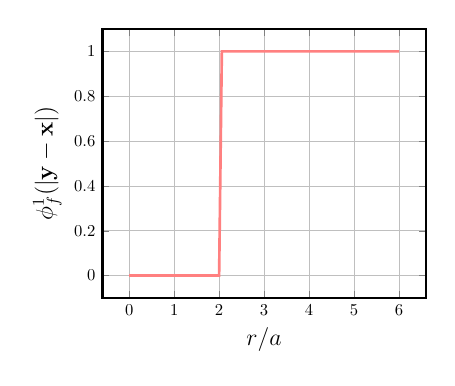
\begin{tikzpicture}[scale=0.6]
    \begin{axis}[
        xlabel={\Large$r/a$},
        ylabel={\Large$\phi_f^1(|\textbf{y}-\textbf{x}|)$},
        legend style={at={(0.05,0.05)}, anchor=south west},
        grid=major,
        domain=0:6,
        samples=100,
        ultra thick
    ]
    
    % Plot for phi = 0.05
    \addplot[color=red!50,ultra thick]
    { x < 2 ? 0 : 1};
    % \addlegendentry{$\phi = 0.05$}
    
    % % Plot for phi = 0.01
    % \addplot[color=blue!50,ultra thick]
    % { exp(-0.01 * (x^3 - 1))};
    % \addlegendentry{$\phi = 0.01$}
    
    % % Plot for phi = 0.001
    % \addplot[color=green!50,ultra thick]
    % { exp(-0.0001 * (x^3 - 1))};
    % \addlegendentry{$\phi = 10^{-4}$}
    
    \end{axis}
\end{tikzpicture}


In that case we must treat the problem into three region 
\paragraph*{First : $|\textbf{y} - \textbf{x}| > 2a$ :} we have $\phi_f^1 = \phi_f$, thus, $\phi_f^{1d} = 0$. same for $\phi_d$
\begin{align*}
    \avg{(\delta_1 - P_1)\rho^0\textbf{w}}
    &=0\\
    \avg{(\delta_1 - P_1)\rho^0\textbf{u}^0} / P_1
    &= 
    % \avg{(\delta_1 - P_1)\rho_f\chi_f\textbf{u}^0_f}
    % \avg{(\delta_1 - P_1)\rho_d\chi_d\textbf{u}^0_d}
    % = 
    \rho_f\phi_f\textbf{u}^{1d}_f
    + 
    \rho_d\phi_d\textbf{u}^{1d}_d
    \\
    \avg{(\delta_1 - P_1)\bm\sigma^0} 
    &= 
    - \phi_f^1 p^{1d}_f\bm\delta P_1 
    +\mu_f P_1 (\grad \textbf{u}^{1d} + \grad \textbf{u}^{1d})
    + \avg{(\delta_1 - P_1) \chi_d\bm\sigma^0_d}
\end{align*}
My guess is $\rho_f\phi_f\textbf{u}^{1d}_f
+ 
\rho_d\phi_d\textbf{u}^{1d}_d = \textbf{u}^{1d}$ 

and indeed we have 
\begin{equation*}
    \avg{\delta_1\textbf{u}^0} - \textbf{u}P_1
    = \avg{\delta_1 \chi_f \textbf{u}_f^0 + \chi_d \textbf{u}_d^0\delta_1 }
    - \textbf{u}_f\phi_fP_1
    - \textbf{u}_d\phi_dP_1
    \approx
    \phi_f^1 \textbf{u}_f^{1d} 
    + \phi_d^1 \textbf{u}_d^{1d}
\end{equation*}

\subsubsection*{Computation of the fluid phase term}

For suspension of spherical particles in the dilute limit the fluid phase averaged fields may be simplyfied by noticing that $\phi_f^1[\textbf{x},t;\textbf{y},\textbf{c}] P_1[\textbf{y},\textbf{c},t] = P_1[\textbf{y},\textbf{c},t]$ when $|\textbf{x} - \textbf{y}| > a$. 
\begin{equation}
    \avg{\chi_f f_f^0}[\textbf{x},t]
    = 
    \int_{\mathbb{R}^3}
    \int_{\mathbb{R}^3}
    f_f^1 \phi_f^1[\textbf{x},t;\textbf{y},\textbf{c}] P_1[\textbf{y},\textbf{c},t]
    d\textbf{y} 
    d\textbf{c}
\end{equation}
where,
\begin{equation*}
    f_f^1 \phi_f^1[\textbf{x},t;\textbf{y},\textbf{c}] P_1[\textbf{y},\textbf{c},t]
    =     
    \int
    \frac{1}{N}
    \sum_\alpha \delta(\textbf{y}-\textbf{x}_\alpha)
     \delta(\textbf{c}-\textbf{u}_\alpha)
    \chi_f
    f^0_f[\textbf{x},t;\FF]
    d\PP.
\end{equation*}

% \section{Introduction}
\label{ap:Closure_problem}

The equations governing the closure problem are often derived based on physical principles or intuitive reasoning.
For example, to determine the drag force term in the averaged momentum equation, in the dilute limit, the problem of a translating sphere in an unbounded flow with background velocity $\textbf{u}^\infty$ is commonly considered \citep{stone2001inertial,raja2010inertial,guazzelli2011}.
"background velocity" refers to the undisturbed flow at the particle location as if the particle were not present.


However, in the context of averaged equations, one might wonder: does $\textbf{u}^\infty$ correspond to the averaged fluid velocity $\textbf{u}_f$ (as used in \citet{jackson1997locally,zhang1997momentum}), the bulk velocity $\textbf{u}$ \citep{kim1985modelling}, or the Favre-averaged velocity $\textbf{u}_m$?
In other words, how can we relate the ensemble-averaged properties of the "hybrid" or "two-fluid" model to the closure terms?

As demonstrated, this question introduces the need for a rigorous statistical derivation of the closure problem.

The closure terms in the ``Hybrid'' model are the results of the ensemble average operator $\avg{\ldots}$. 
In all rigor, we cannot compute theoretically such an average since it necessitates knowing the distribution $P(\FF)$ and the exact expression of the local terms indicated by the notation $(\ldots)^0$. 
In the same spirit as in \citet{buyevich1979flow,lhuillier1992ensemble,batchelor1972sedimentation,hinch1977averaged} and \citet{zhang1994averaged} we demonstrate here that it is therefore necessary to reformulate the closure term to remove the ensemble average procedure. 
We demonstrated in \ref{ap:Closure_problem} that any ensemble-averaged quantities can be reformulated as an integral of what we call \textit{conditionally-averaged quantities}. 
The expressions obtained are  consistent with \citet{batchelor1972sedimentation,hinch1977averaged} and \citet[Appendix A]{zhang1994averaged} which also proposed conditional averages, but somewhat more general because our methodology applies to any closure term of the ``Hybrid model''. 
In a second step, we demonstrate how to derive what we call the \textit{conditionally-averaged equations} that are needed to obtain the \textit{conditionally-averaged quantities}. 

In the limit of Stokes flows \citet{hinch1977averaged} were the first authors to introduce this methodology.
He used the \textit{conditionally-averaged equations} to re-demonstrate, as a proof of concept, the bulk stress of a suspension of solid spheres at $\mathcal{O}(\phi^2)$ and the sedimentation velocity of the dispersed phase at $\mathcal{O}(\phi^2)$. 
In \citet{kim1985modelling} they use the \textit{conditionally-averaged equations} to consider the effect of finite volume fraction on the drag force closure term, in fixed beds of spherical solid spheres, their analysis holds for arbitrary volume fraction $\phi$. 

Again our derivation is directly inspired by the cited author, but the approach is generalized by considering fluid inclusion and an inertial regime. 
For instance, in the dilute regime, the \textit{conditionally-averaged equations} correspond to the problem of the disturbance field generated by an isolated translating droplet. 
The real interest behind this demonstration is that it is kept general and offers many possibilities for model extension.
 




% In \ref{sec:reformulation} and \ref{sec:the_disturbance_eq} we discuss the general approach to derive the closure problem
%%%%%%%%%%%%%%%%%%% A mettre dans lautre chap
% , while in \ref{sec:application} we derive the closures terms of the momentum and energy equations. 
% Since the derivation of the closure terms can be understood through physical arguments, readers who are less interested in the rigorous mathematical formulation of the closure problem, which can be quite involved, may skip directly to \ref{sec:application}.


\section{Reformulation of the closure terms}
\label{sec:reformulation}

% We aim to compute our closures within the dilute Stokes flow regime for spherical particles of radius $a$. 
% In this regime we expect that the closure terms will only be determined by the center of mass velocity of the droplets ($\textbf{u}_p$), their position in space, and the macroscopic properties of the continuous phase ($\textbf{u}_f, \grad \textbf{u}_f \ldots$). 
% Indeed, as we will demonstrate in the following section, only these properties define the boundaries of the \textit{single-particle} conditionally-averaged equations, and are therefore sufficient to achieve closure of the problem  in the Stokes flow regime. 

In the following, we express our closures in terms of averaged quantities, conditioned on the position of the center of mass of a \textit{test-particle} and its center of mass velocity. 
Note that for shape-dependent closure terms it would also be necessary to obtain the \textit{shape-conditioned} averaged fields, but this is out of the scope of this work.
Similarly, to account for the contribution of droplet acceleration to the closure terms (such as the added mass effect), it would be necessary to consider the \textit{center-of-mass-acceleration-conditioned} averaged fields.
However, this lies beyond the scope of the present work.
  
\subsection{Interfacial terms}

In the equations presented in \ref{sec:application} certain closures, such as surface stresses and surface heat fluxes, are expressed in the form of particle-averaged surface integrals. 
Here, we focus on reformulating these terms in terms of \textit{single-particle} conditionally-averaged quantities, which will be defined in the subsequent sections.

As the procedure is similar for all surface particle-averaged terms, let us take the example of the exchange of momentum term appearing in the continuous and dispersed phase averaged momentum equations (\ref{eq:dt_hybrid_rhou_f} and \ref{eq:dt_hybrid_up}). 
From the definition of the particle average we write,
\begin{align}
    \pSavg{\bm\sigma_f^0\cdot\textbf{n}}[\textbf{x},t]
    &= \avg{ \sum_{\alpha=1}^N \delta(\textbf{x}-\textbf{x}_\alpha[t; \FF])
    \int_{\Gamma_\alpha(t,\FF)}
    (\bm\sigma_f^0\cdot\textbf{n})[\textbf{y},t;\FF]
    d\Gamma[\textbf{y}] }
    \label{eq:first_step_reallay}
\end{align}
By writing this integral explicitly, we emphasize that the particle-averaged quantity (left-hand side of \ref{eq:first_step_reallay}) is evaluated at the point \textbf{x}, while the parameter $\textbf{y}$ is used for the integration over the particle's surface.
Recall that $\Gamma_\alpha$ refers to the surface of the droplet $\alpha$ and $\textbf{x}_\alpha$ to the position of the center of mass of that same droplet $\alpha$. 
Thus, the notation $(\bm\sigma_f^0\cdot\textbf{n})[\textbf{y},t;\FF]$ means that we evaluate the local stress as well as the local normal $\textbf{n}$ to the particle surface, at \textbf{y}. 
We now enlarge the domain of integration from $\Gamma_\alpha$ (the surface of the particle $\alpha$) to $\mathbb{R}^3$ with the introduction of the interface indicator function of the particle $\alpha$, namely $\delta(|\textbf{y} - \textbf{x}_\alpha[t,\FF]| - a)$\footnote{Indeed, for spherical particles, we can define the interface indicator function of a single particle using the definition $\delta_\Gamma = \delta(|\textbf{y} - \textbf{x}_\alpha[t,\FF]| - a)$.}. 
It reads,
\begin{multline}
    \pSavg{\bm\sigma_f^0\cdot\textbf{n}}[\textbf{x},t]
    = \\
    \int_{\mathbb{R}^3}
    \avg{
     \sum_{\alpha=1}^N 
     \delta(\textbf{x}-\textbf{x}_\alpha[t \FF])
    \delta(|\textbf{y} - \textbf{x}_{\alpha}[t;\FF]|-a)
    (\bm\sigma_f^0\cdot\textbf{n})[\textbf{y},t;\FF]
    }
    d\textbf{y}. 
    \label{eq:first_step_drag}
\end{multline} 
Since the domain of integration $\mathbb{R}^3$ is now independent of $\FF$, we may substitute the integral and ensemble average operator. 

As mentioned above, we assume that the closure terms are entirely determined by the center of mass velocity of the particles and their position in space. 
Therefore, to include the condition on the particle velocity we introduce the relation 
\begin{equation}
    \int_{\mathbb{R}^3} \delta(\textbf{w} - \textbf{u}_\alpha[\FF,t]) d\textbf{w} = 1,
    \label{eq:Pw_normed}
\end{equation}
where $\textbf{w}$ is the test-particle center of mass velocity in the Eulerian space and $\textbf{u}_\alpha$ is the center of mass velocity within the Lagrangian framework. 
Injecting \ref{eq:Pw_normed} into \ref{eq:first_step_drag} one obtains, 
\begin{multline}
    \pSavg{\bm\sigma_f^0\cdot\textbf{n}}[\textbf{x},t]
    = \\
    \int_{\mathbb{R}^3}
    \int_{\mathbb{R}^3}
    \avg{
     \sum_{\alpha=1}^N 
     \delta(\textbf{x}-\textbf{x}_\alpha[t \FF])
     \delta(\textbf{w} - \textbf{u}_\alpha[\FF,t])
    \delta(|\textbf{y} - \textbf{x}_{\alpha}[t;\FF]|-a)
    (\bm\sigma_f^0\cdot\textbf{n})[\textbf{y},t;\FF]
    }
    d\textbf{y}
    d\textbf{w}. 
    \label{eq:second_step_drag}
\end{multline}
The quantity with the ensemble average operator now represents the average of the local stress $(\bm\sigma_f^0\cdot\textbf{n})[\textbf{y},t;\FF]$ on every configuration where the interface of a droplet is present at \textbf{y} with its center of mass at \textbf{x} and with a center of mass velocity \textbf{w}.


Moreover, since the expression within the ensemble average in \ref{eq:first_step_drag} is identically zero when, $\textbf{x}_\alpha \neq \textbf{x}$, we may replace the interface indicator function such that 
\begin{equation}
    \delta(\textbf{x}-\textbf{x}_\alpha[t,\FF])\delta(|\textbf{y} - \textbf{x}_{\alpha}[t,\FF]|-a) = \delta(\textbf{x}-\textbf{x}_\alpha[t,\FF])\delta(|\textbf{y} - \textbf{x}|-a). 
    \label{eq:from_R3_to_S}
\end{equation}
Since the function $\delta(|\textbf{y} - \textbf{x}|-a)$ is not dependent on $\FF$ it can be taken out of the ensemble average operator, hence reducing the domain of integration from $\mathbb{R}^3$ to $|\textbf{y}-\textbf{x}| = a$ in \ref{eq:first_step_drag}. 
\footnote{For deformable or non-spherical particles, this function may take a more complicated form, since the interface of a deformable or anisotropic particle is not entirely determinate by its center of mass position. 
It is clear that if the position of the interface is conditioned by the exact shape of the interface, then we can always express the interface indicator function as $\delta(f(\textbf{x}))$ where $f$ is a distance function of the shape that may depend on the particle's orientation (for anisotropic particles) or aspect ratio (for slightly deformable ones). 
Anyhow, this approach is generalizable to other kinds of particles, but in this work, we consider only spherical droplets. 
Note that for spheroidal particles as in \ref{chap:deformable} we may write $\delta_{\alpha\Gamma} = \delta((\textbf{y} - \textbf{x}_\alpha[t,\FF])\cdot (\bm\chi_\alpha+\bm\delta)\cdot(\textbf{y} - \textbf{x}_\alpha[t,\FF]) - a^2)$ where we have used the notation of \ref{chap:deformable}
}

Injecting \ref{eq:from_R3_to_S} into \ref{eq:second_step_drag} and using the last remark leads us to the relation 
\begin{equation}
    \pSavg{\bm\sigma_f^0\cdot\textbf{n}}[\textbf{x},t]
    =
    \int_{\mathbb{R}^3}
    P_1[\textbf{x},\textbf{w},t]
    \int_{|\textbf{x}-\textbf{y}|=a}
    (\bm\sigma_f^1 \cdot \textbf{n})[\textbf{y},\textbf{x},\textbf{w},t]
    d\textbf{y}
    d\textbf{w}
    \label{eq:conditionally_averaged}
\end{equation}
where we introduced the definitions, 
\begin{align}
    \bm\sigma^1_f[\textbf{y},\textbf{x},\textbf{w},t]
    % \phi_I^1[\textbf{y}|\textbf{x},\textbf{w},t] 
    % P_1[\textbf{x},\textbf{w},t]
    &= 
    \frac{1}{P_1}
    \avg{
    \sum_\alpha^N 
    \delta(\textbf{x} - \textbf{x}_\alpha[t,\FF])
    \delta(\textbf{w} - \textbf{u}_\alpha[t,\FF])
    % \delta(|\textbf{y} - \textbf{x}_{\alpha}[t,\FF]|-a)
    \bm\sigma_f^0[\textbf{y},t,\FF]
    },
    \label{eq:sigma_f_1}
    \\
    % \phi_I^1[\textbf{y}|\textbf{x},\textbf{w},t] 
    % P_1[\textbf{x},\textbf{w},t]\nonumber\\
    % = 
    % \avg{
    % \sum_\alpha^N 
    % \delta(\textbf{x} - \textbf{x}_\alpha[t,\FF])
    % \delta(\textbf{w} - \textbf{u}_\alpha[t,\FF])
    % \delta(|\textbf{y} - \textbf{x}_{\alpha}[t,\FF]|-a)
    % }\\
    P_1[\textbf{x},\textbf{w},t]
    &= 
    \avg{
    \sum_\alpha^N 
    \delta(\textbf{x} - \textbf{x}_\alpha[t,\FF])
    \delta(\textbf{w} - \textbf{u}_\alpha[t,\FF])
    }. 
\end{align}
% \tb{Since we reduced the surface int the stress isn't any more conditioned by the surface }
% Here $\bm\sigmais the \textit{single-particle} conditionally-averaged local stress of the continuous phase knowing that interface of the particle at $\textbf{x}$ is  present in \textbf{y} and that there is a particle at \textbf{x} with velocity \textbf{w}. 
With this definition, $\bm\sigma^1_f$ is the continuous phase stress, evaluated at $\textbf{y}$ and time $t$, knowing that there is a particle at position $\textbf{x}$ with velocity \textbf{w}, and that the point \textbf{y} is occupied by the surface of the test-particle 
\footnote{
    As $\bm\sigma^1_f$ is conditioned on the variables: $\textbf{y}$, $\textbf{x}$, $\textbf{w}$, $t$, and evaluated at the position $\textbf{y}$ and time $t$, we should write: $\bm\sigma^1_f[\textbf{y},t|\textbf{x},\textbf{y},\textbf{w},t]$ instead of $\bm\sigma^1_f[\textbf{x},\textbf{y},\textbf{w},t]$.
    However the second notation will be used as a short hand. 
}.
% $\phi_I^1[\textbf{y}|\textbf{x},\textbf{w},t] $ is the probability of finding the interface of the particle at the location \textbf{y} knowing its center of mass is located at \textbf{x}. 
% For identical spherical particles we can write $\phi_I^1[\textbf{y}|\textbf{x},\textbf{w},t] = \delta(|\textbf{x} - \textbf{y}| -a)$.
% That is why the domain of integration over \textbf{y} in \ref{eq:conditionally_averaged} is reduced to $|\textbf{x} - \textbf{y}| < a$. 
$P_1[\textbf{x},\textbf{w},t]$ is the probability of finding a particle center of mass at \textbf{x} with velocity \textbf{w} at time $t$.
This distribution can be decomposed such that $P_1[\textbf{x},\textbf{w},t] = n_p[\textbf{x},t] P_1[\textbf{w}|\textbf{x},t]$ where $n_p$ is the number density evaluated at \textbf{x}, and $P_1$ the probability density of having a particle with velocity \textbf{w} knowing its center of mass location is \textbf{x}. 
Note that this distribution is normed 
\begin{equation*}
    \int_{\mathbb{R}^3} P_1[\textbf{w}|\textbf{x},t] d \textbf{w} = 1. 
\end{equation*}
Finally, note that in \ref{eq:conditionally_averaged} the droplet shape and the position of its center of mass fully determine the normal vector $\textbf{n}$, allowing it to be taken outside the ensemble average. 


\subsubsection{Single-particle conditionally averaged quantities}

All quantities denoted with the superscript $^1$ refer to \textit{single-particle} conditionally-averaged quantities. 
These quantities are conditionally averaged based on the presence of a particle located at \textbf{x} with velocity \textbf{w}.
Additionally, in the following, we will use the shorthand,
\begin{equation}
    \delta_1[\textbf{x},\textbf{w},t,\FF]  \text{ for } \sum_\alpha \delta(\textbf{x} - \textbf{x}_\alpha[t,\FF]) \delta(\textbf{w} - \textbf{u}_\alpha[t,\FF]). 
    \label{eq:delta_1}
\end{equation}  
Thus, we can define the \textit{single-particle} conditional-average of a local quantity $f^0$, as 
\begin{equation}
    f^1[\textbf{y}|\textbf{x},\textbf{w},t] P_1[\textbf{x},\textbf{w},t] = \avg{\delta_1 f^0[\textbf{y},\FF,t]}.
\end{equation}
Such that $f^1$ is the averaged value of $f^0$ at \textbf{y} knowing that there is a particle at \textbf{x} with velocity \textbf{w}. 
If $f_k$ is a quantity defined in the phase $k$ we may write 
\begin{equation*}
    f^1_k[\textbf{y}|\textbf{x},\textbf{w},t] \phi_k^1[\textbf{y}|\textbf{x},\textbf{w},t]  P_1 = \avg{\delta_1 (\chi_k f^0_k) [\textbf{y},\FF,t]}.
\end{equation*}
Such that $\phi_k^1$ is the probability of finding the phase $k$ at \textbf{y} knowing a particle is located at \textbf{w} with velocity \textbf{w}, and $f_k^1$ the conditional average of $f_k^0$. 
For example, we define the \textit{single-particle conditioned average} of the continuous phase velocity fields by, 
\begin{equation*}
    \textbf{u}_f^1 \phi_f^1 P_1
    = \avg{\delta_1 \chi_f \textbf{u}_f^0}
\end{equation*} 
where $\phi_f^1$ is the probability of finding the continuous phase at \textbf{y} knowing a particle is present at \textbf{x} with velocity \textbf{w}. 
$\textbf{u}_f^1$ is the averaged local velocity evaluated at \textbf{y} knowing the continuous phase is present at \textbf{y} with a particle at \textbf{x} having velocity \textbf{w}. 

The stress present in \ref{eq:conditionally_averaged} can now be expressed in terms of conditionally-averaged velocity and pressure fields. 
We use the constitutive law of Newtonian fluids, $\bm\sigma_f^0 = -p_f^0 \bm\delta + \mu_f [\pddy \textbf{u}_f^0+ (\pddy \textbf{u}_f^0)^\dagger]$, with $\pddy$ the gradient over the \textbf{y} coordinate.
Injecting this law into \ref{eq:sigma_f_1} we obtain directly 
\begin{equation}
    \bm\sigma_f^1
    = - p_f^1 \bm\delta
    +\mu_f [\pddy \textbf{u}_f^1+(\pddy \textbf{u}_f^1)^\dagger], 
    \label{eq:sigma_f_surf}
\end{equation}
since $\delta_1$ is independent of \textbf{y}, meaning that it could be permuted with the gradient operator in \ref{eq:sigma_f_surf}. 
Note that this relation is valid only because $\bm\sigma_f^1$ is conditioned on the presence of an interface at \textbf{y} in \ref{eq:sigma_f_1}. 
In conclusion, the ensemble averaged exchange of momentum term can be expressed as the surface integral of the Newtonian stress defined based on the \textit{single-particle} conditional-averaged fields: $\textbf{u}_f^1$, and $p_f^1$. 

It must be understood that this definition \eqref{eq:sigma_f_surf} is only true because the stress is evaluated at the surface of the droplet, in the general case we have, 
\begin{equation}
    P_1 \phi_f^1 \bm\sigma_f^1
    =
    \avg{\delta_1 \chi_f \bm\sigma_f^0}
    =
    P_1 \phi_f^1 p_f^1
    +  \avg{\delta_1\chi_f \{ - p_f^0 \bm\delta + \mu_f [\pddy \textbf{u}_f^0+  (\pddy \textbf{u}_f^0)^\dagger]\}}. 
    \label{eq:sigme_f_1_all_space}
\end{equation}
Note the presence of $\chi_f$ in this expression, in opposition to \ref{eq:sigma_f_surf} where only $\delta_1$ where present.
This is because \ref{eq:sigme_f_1_all_space} is evaluated at an arbitrary point \textbf{y}, while in \ref{eq:sigma_f_surf} we consider only the points lying on the droplet interface.  
From this expression, we can propose two formulations for the continuous phase stress,   
\begin{align}    
    \bm\sigma_f^1
    &= 
    - p_f^1 \bm\delta 
    + \mu_f [\pddy \textbf{u}_f^1+ (\pddy \textbf{u}_f^1)^\dagger ]
    - \frac{\mu_f }{P_1 \phi_f^1}\avg{\delta_1 \delta_\Gamma (\textbf{n}_d \textbf{u}_f''+  \textbf{u}_f'' \textbf{n}_d)},
    \label{eq:sigma_f_surf15}
    \\
    \bm\sigma_f^1
    &= 
    - p_f^1 \bm\delta 
    + \frac{\mu_f }{\phi_f^1} [\pddy \textbf{u}^1+ (\pddy \textbf{u}^1)^\dagger ]
    - \frac{\mu_f }{\phi_f^1} \phi_d^1 \textbf{e}_d^1. 
    \label{eq:sigma_f_surf2}
\end{align}
Where we have defined $\textbf{u}_f'' = \textbf{u}_f^0 - \textbf{u}_f^1$. 
These two expressions can be derived using a similar methodology than for the derivation of \ref{eq:second_form,eq:first_form}. 
Note that the second term on the right-hand side of \ref{eq:sigma_f_surf2} vanishes for solid particles, the rate of strain within solid particle is null.
While the second term of \ref{eq:sigma_f_surf15} does not necessarily vanish. 
That is why the second expression is preferred for solid particles. 

% Additionally, multiplying \ref{eq:sigma_f_surf15} and \ref{eq:sigma_f_surf2} by $\phi_f^1$ and subtracting both expressions gives, 
% \begin{equation} 
%     \frac{1}{P_1}\avg{\delta_1 \delta_\Gamma (\textbf{n}_d \textbf{u}_f''+  \textbf{u}_f'' \textbf{n}_d)}
%     -  \phi_d^1 \textbf{e}_d^1
%     = 
%     [(\textbf{u}_f^1 - \textbf{u}_d^1)\pddy\phi_d^1+ \pddy \phi_d^1(\textbf{u}_f^1 - \textbf{u}_d^1) ]
%     - \phi_d^1 [\pddy\textbf{u}_d^1+  (\pddy \textbf{u}_d^1)^\dagger ]. 
% \end{equation}
% For ensemble averaged (not conditionally-averaged) quantities we can equally show that
% \begin{multline} 
%     \avg{\delta_\Gamma (\textbf{n}_d \textbf{u}_f'+  \textbf{u}_f' \textbf{n}_d)}
%     - \phi_d \textbf{e}_d
%     = 
%     +  [(\textbf{u}_f - \textbf{u}_d)\pddy\phi_d+ \pddy \phi_d(\textbf{u}_f - \textbf{u}_d) ]
%     - \phi_d [\pddy\textbf{u}_d+  (\pddy \textbf{u}_d)^\dagger ]
% \end{multline}
% Note that for solid particles this relation can directly lead us to a closure for the surface term on the left-hand side, namely
% \begin{multline} 
%     \avg{\delta_\Gamma (\textbf{n}_d \textbf{u}_f'+  \textbf{u}_f' \textbf{n}_d)}
%     = 
%     [(\textbf{u}_f - \textbf{u}_d)\pddy\phi_d+ \pddy \phi_d(\textbf{u}_f - \textbf{u}_d) ]
%     - \phi_d [\pddy\textbf{u}_d+  (\pddy \textbf{u}_d)^\dagger ]. 
%     \label{eq:closure_un_nu}
% \end{multline}

\begin{figure}[h!]
    \centering
    \includegraphics[width=0.2\textheight]{image/dist_phi.pdf}
    \caption{Representation of a possible form for the probability of finding the dispersed phase at \textbf{x} knowing a spherical particle of radius $a$ is present at $\textbf{y}$.
    Note the zone empty of particle concentration near the points $|\textbf{x}- \textbf{y}|=a$, this due to the impenetrability of particles. 
    }
    \label{fig:distrib}
\end{figure}
At the surface of the test-particle, the probability of finding the dispersed phase, i.e. finding the dispersed phase in contact with the surface of the reference particle, is identically null (not to be confused with the probability of finding another droplet center of mass). 
Indeed, a thin film of continuous phase always separates the droplet surface from its neighbors (see \ref{fig:distrib}).
Therefore, we may write $\phi_d^1 = 0$ at $|\textbf{x}- \textbf{y}| =a$. 
Thus, when evaluated at the subsurface of the particle, we can use the relation $\textbf{u}_f^1 = \textbf{u}^1$ and $p_f^1 = p^1$. 
Consequently, to compute the surface stress of a particle, either the conditionally-averaged quantities of the continuous phase ($\textbf{u}_f^1, p_f^1$) or the bulk quantities ($\textbf{u}^1$, $p^1$) are required. 
Another consequence of this is that, the definitions given by, \ref{eq:sigma_f_surf15}, \ref{eq:sigma_f_surf2}, or \ref{eq:sigma_f_surf} are all consistent when evaluated at the points located on the surface of the droplet at \textbf{x}. 

\subsection{Mean fields and disturbance fields contribution}

As it is often done in the literature \citep{zhang1994ensemble,jackson2000,wang2021numerical,wang2024effect}, we would like to separate the averaged momentum exchange into a contribution from the mean flow and pressure fields, and the contribution arising due to the disturbance velocity and pressure fields.  

\subsubsection{Definitions}

In the first place, we need to define what is a disturbance field.
Let us take the example of the conditioned velocity field, $\textbf{u}_f^1$, and its corresponding disturbance velocity field.
We state that the conditioned field, $\textbf{u}_f^1$, is equivalent to the ensemble-averaged velocity field $\textbf{u}_f$ when the particle at \textbf{x} is sufficiently far from the point where the velocity $\textbf{u}_f^1$ is evaluated (the point \textbf{y}).
Thus, we write,  
\begin{equation}
    \lim_{|\textbf{y}-\textbf{x}|\to\infty} 
    \textbf{u}_f^1[\textbf{y},\textbf{x},\textbf{w},t]
    =
    \textbf{u}_f[\textbf{y},t]. 
    \label{eq:lim_u_1}
\end{equation} 
Note that this definition requires an infinitely large domain. 
This implies that the solutions obtained in the subsequent sections are restricted to infinitely large domains, devoid of boundary conditions.

Let us assume that $L$ is the macroscopic length scale of our process and that $a$  is the typical size of the particles.
Since the particle-size scale $a$ is much smaller than the boundary length scale $L$ we assume that $\textsc{O}(a/L)$ is negligible. 
In the worth case scenario, the disturbance field of a droplet is $(\textbf{u}_f^1- \textbf{u}_f)\sim a/|\textbf{y}-\textbf{x}|$ \citet{kim2013microhydrodynamics}.
Hence, in a physical situation where $|\textbf{y}-\textbf{x}|\to L$ instead of $|\textbf{y}-\textbf{x}|\to\infty$ in \ref{eq:lim_u_1} we may estimate that the error is of $\mathcal{O}(a/L)$, hence negligible upon a reasonable separation of scale.
However, it is interesting to note that this will no longer be the case for other problems such as sediment transport for examples.
In this case, the boundary condition, i.e. the top of the particle bed and the ground, are at a distance of the same length scale as the particle-size. 

In light of \ref{eq:lim_u_1}, we define the disturbance velocity field as 
\begin{equation}
    \textbf{u}_f^{1d}
    =
    \textbf{u}_f^1 
    - 
    \textbf{u}_f. 
    \label{eq:def_u_1d}
\end{equation}
because it satisfies the definition, 
\begin{equation}
    \lim_{|\textbf{y}-\textbf{x}|\to\infty} 
    \textbf{u}_f^{1d}[\textbf{y},\textbf{x},\textbf{w},t]
    =
    \lim_{|\textbf{y}-\textbf{x}|\to\infty} 
    \{\textbf{u}_f^1[\textbf{y},\textbf{x},\textbf{w},t]
    - \textbf{u}_f[\textbf{y},t]\}
    = 0.
    \label{eq:lim_u_1d}
\end{equation} 
Thus, $\textbf{u}_f^{1d}$ tends to zero at large distances from the particle, which is consistent with the terminology ``disturbance''.
The definition \ref{eq:def_u_1d} can apply to any \textit{conditional-averaged} quantities $f^1$, we define
\begin{equation}
    \lim_{|\textbf{y}-\textbf{x}|\to\infty} 
    \{f_f^1[\textbf{y},\textbf{x},\textbf{w},t]
    - f_f[\textbf{y},t]\}
    =
    f_f^{1d}[\textbf{y},\textbf{x},\textbf{w},t]
    = 0.
\end{equation} 

\subsubsection{Momentum exchange decomposition}

Using the decomposition $\bm\sigma_f^1 = \bm\sigma_f^{1d} + \bm\sigma_f$ in \ref{eq:conditionally_averaged} we finally introduce the decomposition of the averaged momentum exchange term as:  
\begin{align}
    \pSavg{\bm\sigma_f^0\cdot\textbf{n}}[\textbf{x},t]
    =
    n_p[\textbf{x},t]
    \int_{|\textbf{x}-\textbf{y}|=a}
    \bm\sigma_f[\textbf{y},t]
    \cdot \textbf{n}
    d\textbf{y}
    \nonumber
    \\
    + 
    \int_{\mathbb{R}^3}
    P_1[\textbf{x},\textbf{w},t]
    \int_{|\textbf{x}-\textbf{y}|=a}
    \bm\sigma_f^{1d}[\textbf{y},\textbf{x},\textbf{w},t]
    \cdot \textbf{n}
    d\textbf{y}
    d\textbf{w}
    \label{eq:general_partition}
\end{align}
where the first term represents the contribution from the mean continuous phase stress, $\bm\sigma_f$, and the second term is the contribution from the disturbance fields stress $\bm\sigma_f^{1d}$. 
While this decomposition is arbitrary since $\bm\sigma_f^1$ could be partitioned into other arbitrary tensors, it enables by definition, the separation of the mean flow contribution, $\bm\sigma_f$, from the stress induced by the local-scale disturbance fields, $\bm\sigma_f^{1d}$.
This decomposition is used by \citet[Chapter 2]{jackson2000} and \citet{zhang1997momentum,wang2021numerical,wang2024effect} for suspensions of solid spheres, although these authors do not explicitly provide the expression for the tensor $\bm\sigma_f^{1d}$, which we aim to derive in the following sections. 

Note that $\bm\sigma_f$ is evaluated at $\textbf{y}$ in \ref{eq:general_partition}. 
Although $\bm\sigma_f$ is ensemble-averaged, we emphasize that it may still depend on the position in inhomogeneous flows. 
Assuming the suspension is slightly non-homogeneous \citep{lhuillier1992ensemble}, we have $\bm\sigma_f[\textbf{y},t] = \bm\sigma_f[\textbf{x},t] + \textbf{r}\cdot \nabla\bm\sigma_f[\textbf{x},t] + \ldots$, where $\textbf{r} = \textbf{y} - \textbf{x}$. 
By retaining only the first three terms in the expansion, we can demonstrate that
\begin{equation}
    \pSavg{\bm\sigma_f^0\cdot\textbf{n}}
    =
    n_p v_p 
    \div\bm\sigma_f
    +
    \int_{\mathbb{R}^3}
    P_1
    \int_{|\textbf{x}-\textbf{y}|=a}
    \bm\sigma_f^{1d} \cdot \textbf{n}
    d\textbf{y}d\textbf{w}.
    \label{eq:drag_final}
\end{equation}
Therefore, the total momentum exchange term contains a component related to the divergence of the mean fluid-phase stress, in addition to the contribution from the disturbance fields. 
Similar arguments can be extended to the first two moments of the hydrodynamic force. 
These expressions can be written as:
\begin{align}
    \pSavg{\textbf{r}\bm\sigma_f^0\cdot\textbf{n}}
    &=
    n_p v_p \bm\sigma_f
    +
    \int_{\mathbb{R}^3}
    P_1
    \int_{|\textbf{x}-\textbf{y}|=a}
    \textbf{r}\bm\sigma_f^{1d} \cdot \textbf{n}
    d\textbf{y}
    d\textbf{w},
    \label{eq:first_mom_general}
    \\
    \pSavg{\textbf{rr}\bm\sigma_f^0\cdot\textbf{n}}
    &=
    n_pv_p  \frac{a^2}{5} 3 [(\div \bm\sigma_f)\bm\delta]^\text{sym}
    +
    \int_{\mathbb{R}^3}
    P_1
    \int_{|\textbf{x}-\textbf{y}|=a}
    \textbf{rr}\bm\sigma_f^{1d} \cdot \textbf{n}
    d\textbf{y}
    d\textbf{w},
    \label{eq:second_mom_general}
\end{align}
where the operator $[\ldots]^\text{sym}$ returns the symmetric part of the arguments. 
It is important to note that the contribution from the mean stress in the second moment of the hydrodynamic force may become negligible when a proper separation of scale is considered. 
Indeed, this term is proportional to $a^2$ \eqref{eq:second_mom_general}, and it appears under the operator $\grad\grad\sim L^{-2}$ in the averaged momentum equation \ref{eq:dt_hybrid_rhou_f}, hence contributing to $\mathcal{O}(a^2/L^2)$, which may be considered as negligible. 

According to the expressions \ref{eq:drag_final}, \ref{eq:first_mom_general}, and \ref{eq:second_mom_general}, we will need to compute the term $\bm\sigma^{1d}_f = \bm\sigma_f^1 - \bm\sigma_f$ where $\bm\sigma_f^1$ is given by \ref{eq:sigma_f_surf}. 
Regarding the mean continuous phase stress we recall that it can be written in two ways (see \ref{chap:daniel15}), namely 
\begin{align}
    \label{eq:mean_continuous_phase_stress}
    \bm\sigma_f
    &= - p_f \bm\delta 
    + \mu_f [\pddy \textbf{u}_f+ (\pddy \textbf{u}_f)^\dagger ]
    - \frac{\mu_f}{\phi_f}\avg{\delta_\Gamma (\textbf{n}_d \textbf{u}_f'+  \textbf{u}_f' \textbf{n}_d)}, \\
    \bm\sigma_f
    &= - p_f \bm\delta 
    + \frac{\mu_f}{\phi_f} [\pddy \textbf{u}+ (\pddy \textbf{u})^\dagger ]
    - \frac{\mu_f \phi_d}{\phi_f} \textbf{e}_d
    \label{eq:mean_continuous_phase_stress2}
\end{align}
Thus using \ref{eq:sigma_f_surf} and \ref{eq:mean_continuous_phase_stress} we find for the points on the particle's surface ($|\textbf{y}-\textbf{x}| = a$) that,
\begin{align}
    \bm\sigma_f^{1d}
    =
    - p_f^{1d} \bm\delta 
    + \mu_f [\pddy \textbf{u}_f^{1d}+ (\pddy \textbf{u}_f^{1d})^\dagger ]
    + \frac{\mu_f }{\phi_f}\avg{\delta_\Gamma (\textbf{n}_d \textbf{u}_f'+  \textbf{u}_f' \textbf{n}_d)}. 
    \label{eq:sigma_explict}
\end{align}
Thus, according to \ref{eq:sigma_explict}, the disturbance stress that is integrated over the particle surface in \ref{eq:drag_final} to \ref{eq:second_mom_general}, is not only the Newtonian stress-like contribution of the disturbance fields ($\textbf{u}_f^1$ and $p_f^1$), but also includes the contribution of the term $\avg{\delta_\Gamma (\textbf{n}_d \textbf{u}_f'+  \textbf{u}_f' \textbf{n}_d)}$. 
Thus, in the force closures: \ref{eq:drag_final} and \ref{eq:first_mom_general}, we will observe the appearance of the terms involving the divergence of $\avg{\delta_\Gamma (\textbf{n}_d \textbf{u}_f'+  \textbf{u}_f' \textbf{n}_d)}$ times $n_pv_p$, and  $n_pv_p \avg{\delta_\Gamma (\textbf{n}_d \textbf{u}_f'+  \textbf{u}_f' \textbf{n}_d)}$, respectively. 
These terms will ultimately cancel out their corresponding contributions in $\bm\sigma_f$ that appear on the left-hand side of \ref{eq:drag_final} and \ref{eq:first_mom_general}. 

To provide a better understanding for the following discussion we remark that for solid particles $\textbf{e}_d = 0$. 
Therefore, subtracting \ref{eq:mean_continuous_phase_stress} from \ref{eq:mean_continuous_phase_stress2}, gives directly, 
\begin{equation}
    \avg{\delta_\Gamma (\textbf{n}_d \textbf{u}_f'+  \textbf{u}_f' \textbf{n}_d)}
    = 
    (\textbf{u}_f - \textbf{u}_d)\pddy \phi_d + \pddy \phi_d (\textbf{u}_f - \textbf{u}_d)
    -  \phi_d [\pddy \textbf{u}_d+ (\pddy \textbf{u}_d)^\dagger ]. 
    \label{eq:closure_un_nu}
\end{equation} 
Therefore, at least for solid particles, this term is non-zero as soon as there are non-negligible gradients of volume fraction and mean gradients of particle velocities. 


We conclude that the commonly used decomposition of the drag force introduced by \citet{zhang1997momentum,jackson2000}, given by \ref{eq:general_partition}, requires adding the term  $\avg{\delta_\Gamma (\textbf{n}_d \textbf{u}_f'+  \textbf{u}_f' \textbf{n}_d)}$ to the classical Newtonian stresses in the second term of \ref{eq:general_partition} and subtracting it in the mean drag force term (first term of \ref{eq:general_partition}). 
This finding implies that, in the recent work of \citet{wang2021numerical, wang2024effect}, where this decomposition is employed for the drag force, we assert that they have actually computed the integral of the first two terms of \ref{eq:sigma_explict}, while neglecting the final term. 
Interestingly, \citet{wang2024effect} specifically investigates the effect of the volume fraction gradient ($\grad \phi_d$) on the drag force. 
In this context, it is clear from \eqref{eq:closure_un_nu} that the term $\avg{\delta_\Gamma (\textbf{n}_d \textbf{u}_f'+  \textbf{u}_f' \textbf{n}_d)}$ cannot be neglected. 
Only when the analysis is accurate to $\mathcal{O}(\phi_d)$ does this term vanish in \ref{eq:drag_final}, reducing \ref{eq:sigma_explict} to the Newtonian stress expression. 
% Thus, the drag force computed in the DNS of \citet{wang2024effect} may not be the one defined in their momentum equations. 

Note that using \ref{eq:mean_continuous_phase_stress2} instead of \ref{eq:mean_continuous_phase_stress} in \ref{eq:sigma_explict} and switching $\textbf{u}_f^1$ and $\textbf{u}^1$ in \ref{eq:sigma_f_surf}, does not solve this inconsistency. 

\subsubsection{An alternative stress decomposition}

As the previous decomposition requires adding and subtracting $\avg{\delta_\Gamma (\textbf{n}_d \textbf{u}_f'+  \textbf{u}_f' \textbf{n}_d)}$ in each term of \ref{eq:general_partition}, we decide to avoid this overcomplicated operation and introduce, the partitioning 
\begin{equation}
    \bm\sigma_f^1 =
    \bm\Sigma_f + 
    \bm\Sigma_f^{1d}. 
    \label{eq:mean_Newtonian}
\end{equation}
Where the mean stress and disturbance stresses are defined as, 
\begin{align}
    \bm\Sigma_f^{1d}
    &=-p_f^{1d}\bm\delta + \mu_f^1 [\grad \textbf{u}^{1d}_f + (\grad \textbf{u}^{1d}_f)^\dagger], \\
    \bm\Sigma_f
    &=-p_f\bm\delta + \mu_f^1 [\grad \textbf{u}_f + (\grad \textbf{u}_f)^\dagger], 
\end{align}
respectively. 
Note that the use of $\textbf{u}_f$ as the ensemble-averaged velocity of reference is arbitrary.
Indeed, recall that at the surface of the test particle we have $\phi_d^1=0$, hence $\textbf{u}_f^1 = \textbf{u}^1$. 
Thus, at the surface of the test-particle, one could use the decomposition,
\begin{equation}
    \bm\sigma_f^1 =
    \bm\Sigma + 
    \bm\Sigma^{1d}. 
    \label{eq:mean_Newtonian2}
\end{equation}
Where the mean stress and disturbance stresses are defined as, 
\begin{align}
    \bm\Sigma^{1d}
    &=-p_f^{1d}\bm\delta + \mu_f^1 [\grad \textbf{u}^{1d} + (\grad \textbf{u}^{1d})^\dagger], \\
    \bm\Sigma
    &=-p_f\bm\delta + \mu_f^1 [\grad \textbf{u} + (\grad \textbf{u})^\dagger]. 
\end{align}
One could wonder which of these stress decomposition (\ref{eq:mean_Newtonian2} or \ref{eq:mean_Newtonian}) is the more efficient? 
The answer is that it depends on the unknown of the problem at hand. 
If we consider an averaged system of equations for the mean continuous phase field $\textbf{u}_f$ then, \ref{eq:mean_Newtonian} seems more adapted, however, if the unknown is \textbf{u}, then \ref{eq:mean_Newtonian2} is more adapted. 
In all case since $\textbf{u} = \textbf{u}_f + \phi_d (\textbf{u}_d - \textbf{u}_f)$ one can always recover \ref{eq:mean_Newtonian2} from \ref{eq:mean_Newtonian} or inversely.




Using the same methodology as in the previous manipulations we re-write the force closures as, 
\begin{align}
    \pSavg{\bm\sigma_f^0\cdot\textbf{n}}
    &=
    n_p v_p 
    \div\bm\Sigma_f
    +
    \int_{\mathbb{R}^3}
    P_1
    \int_{|\textbf{x}-\textbf{y}|=a}
    \bm\Sigma_f^{1d} \cdot \textbf{n}
    d\textbf{y}d\textbf{w}
    \label{eq:drag_final2}\\
    \pSavg{\textbf{r}\bm\sigma_f^0\cdot\textbf{n}}
    &=
    n_p v_p \bm\Sigma_f
    +
    \int_{\mathbb{R}^3}
    P_1
    \int_{|\textbf{x}-\textbf{y}|=a}
    \textbf{r}\bm\Sigma_f^{1d} \cdot \textbf{n}
    d\textbf{y}
    d\textbf{w}
    \\
    \pSavg{\textbf{rr}\bm\sigma_f^0\cdot\textbf{n}}
    &=
    n_pv_p  \frac{a^2}{5} 3 [(\div \bm\Sigma_f)\bm\delta]^\text{sym}
    +
    \int_{\mathbb{R}^3}
    P_1
    \int_{|\textbf{x}-\textbf{y}|=a}
    \textbf{rr}\bm\Sigma_f^{1d} \cdot \textbf{n}
    d\textbf{y}
    d\textbf{w}
    \label{eq:second_mom_general2}
\end{align}
This decomposition, though perhaps less natural, appears to be more physically meaningful. 
Indeed, unlike the previous approach, the mean contribution no longer depends on the mean relative motion through the term $\avg{\delta_\Gamma (\textbf{n}_d \textbf{u}_f'+  \textbf{u}_f' \textbf{n}_d)}$ in $\bm\sigma_f$ (see \ref{eq:closure_un_nu}), but solely on the mean fluid phase properties $p_f$ and $\textbf{u}_f$, while the local stress is a Newtonian-like stress.  

The main take-away of this section is that: (1)  the particle-averaged force traction terms can be computed based on the knowledge of $p_f^{1d}$ and $\textbf{u}_f^{1d}$. 
These fields can be obtained by solving the corresponding disturbance field equations. 
Note that one may also compute the mixture properties $p^{1d}$ and $\textbf{u}^{1d}$ and then use the relation $p_f^{1d} = p^{1d} + \phi_d (p_f - p_d)$ or $\textbf{u}_f^{1d} = \textbf{u}^{1d} + \phi_d (\textbf{u}_f - \textbf{u}_d)$. 
And (2) the force decomposition often used \citep{jackson2000,zhang1997momentum,wang2021numerical,wang2024effect} seems inconsistent compared to the drag force computed in the cited studies.
Indeed, it is likely that their definition of the ``drag force'' term, requires the subtraction of a term proportional to the particle volume fraction. 
This inconsistency is settled by re-defining the forces partition.  

\subsection{Particle phase volumic terms}

Some closure terms such as the particle internal stress $\pOavg{\bm{\sigma}_2^0}$ or the particle internal dissipation term $\pOavg{\bm{\sigma}_2^0:\grad \textbf{u}_d^0}$ are particle-averaged volume integral of locals quantities. 
In this situation the reformulation is slightly different since we must consider volume and not the surfaces of the particle.  Nevertheless the approach is similar. 
For the particle internal stress we can write, 
\begin{equation}
    \pOavg{\bm\sigma_d^0}[\textbf{x},t]
    =
    \int_{\mathbb{R}^3}
    P_1[\textbf{x},\textbf{w}]
    \int_{|\textbf{x}-\textbf{y}|<a}
    \bm\sigma_d^1[\textbf{y},t;\textbf{x},\textbf{w}] 
    d\textbf{y}
    d\textbf{w}. 
    \label{eq:conditionally_averaged_vol}
\end{equation}
Assuming a Newtonian fluid for the particles, $\bm\sigma_d^0 = -p_d^0 \bm\delta + \mu_d [\nabla \textbf{u}_d^0 + (\nabla \textbf{u}_d^0)^\dagger]$, and given that within the region $|\textbf{x} - \textbf{y}| < a$, only the dispersed phase is present.
This allows the permutation between ensemble averages and derivatives.
We can express this as:
\begin{equation}
    \bm\sigma_d^1  
    = 
    -p_d^1   \bm\delta
    + \mu_d  [\pddy \textbf{u}^1_d+(\pddy  \textbf{u}^1_d)^\dagger],
    \label{eq:dispersed_phase_stress}
\end{equation}
which is simply the expression of the Newtonian stress within the particle centered at \textbf{x}, based on the mean fields $p_d^1$ and $\textbf{u}_d^1$. 
As in the previous section, one can eventually partition this conditional stress into an ensemble averaged stress plus a local disturbance field. 

\subsection{Continuous phase closures}

The closure terms of the form $\avg{\chi_f f_f^0}$ differ in their mathematical structure, as they represent an average over the continuous phase rather than the dispersed phase. 
Consequently, the reformulation method is slightly different and requires additional assumptions. Two examples of such terms are the Reynolds stress $\avg{\chi_f \textbf{u}_f'\textbf{u}_f'}$ and the fluid-phase dissipation $\avg{\chi_f \bm\sigma_f^0 : \nabla \textbf{u}_f^0}$, which appear in \ref{eq:dt_hybrid_rhou_f} and \ref{eq:dt_hybrid_k1}, respectively.  

We first note that, 
\begin{equation}
    \frac{1}{N}\sum_\alpha^N
    \int_{\mathbb{R}^3}
    \int_{\mathbb{R}^3}
    \delta(\textbf{y}-\textbf{x}_\alpha[\FF,t])
    \delta(\textbf{w}-\textbf{u}_\alpha[\FF,t])
    d\textbf{x}
    d\textbf{w}
    = 1,
\end{equation}
where $N$ is the total number of particles in the flow. 
Using this relation one may re-formulate the ensemble average of a continuous phase quantity as 
\begin{equation}
    \phi_f f_f[\textbf{x},t]
    = 
    \frac{1}{N}
    \int_{\mathbb{R}^3}
    \int_{\mathbb{R}^3}
    f_f^1[\textbf{x},\textbf{y},\textbf{w},t] \phi_f^1[\textbf{x}|\textbf{y},\textbf{w},t]  P_1[\textbf{y},\textbf{w}] 
    d\textbf{y} 
    d\textbf{w}
    \label{eq:conditional_averaged_fluid}
\end{equation}
where,
\begin{equation*}
    f_f^1[\textbf{x},\textbf{y},\textbf{w},t] \phi_f^1[\textbf{x}|\textbf{y},\textbf{w},t]  P_1[\textbf{y},\textbf{w}]
    =     
    \avg{
    \sum_\alpha^N 
    \delta(\textbf{y}-\textbf{x}_\alpha[\FF,t])
     \delta(\textbf{w}-\textbf{u}_\alpha[\FF,t])
    (\chi_f
    f^0_f)[\textbf{x},t;\FF]
    }.
\end{equation*}
In this expression $f_f^1[\textbf{x},t;\textbf{y},\textbf{w}]$ is the average of the local quantity $f_f^0$ evaluated at $\textbf{x}$ and time $t$ conditionally on, the presence of the continuous phase at \textbf{x}, and a particle center of mass at $\textbf{y}$ with center of mass velocity $\textbf{w}$. 
Similarly, $\phi_f^1[\textbf{x},t|\textbf{y},\textbf{w}]$ is the fluid phase volume fraction at \textbf{x} and time $t$, conditionally on the presence of a particle at $\textbf{y}$ with center of mass velocity \textbf{w}. 
Note that for $|\textbf{x} - \textbf{y}| < a$, $\phi_f^1[\textbf{y}|t,\textbf{x},\textbf{w}] = 0$ however at, 
$\lim_{|\textbf{x} - \textbf{y}| \to \infty} \phi_f^1 = \phi_f$. 
Note that this derivation is consistent with (2.21) and (2.22) of \citet{zhang1994ensemble} with $K = 1$. 

This, formulation remains quite general and is valid regardless of the flow regime, however, the presence of the term $N$ makes this formulation unpractical. 
Indeed, $P_1 = n_p[\textbf{y},t] P_1[\textbf{w}|\textbf{y},t]$ and $n_p[\textbf{y},t] /N = V_\Omega$, where $V_\Omega$ is the volume of the whole domain. 
Thus, substituting  $n_p[\textbf{y},t] /N = V_\Omega$ into \ref{eq:conditional_averaged_fluid} transforms the right-hand side of this relation to a volume average over $V_\Omega$ of a property evaluated at \textbf{x} on all possible particles positions in $V_\Omega$.  
Anyhow, \ref{eq:conditional_averaged_fluid} requires macroscopic information such as $N$ and $V_\Omega$, which we do not necessarily have if our goal is to compute general closure formulation. 
This is because, contrary to particle-averaged quantities, we could not consider a contribution per particle that is holds fixed at \textbf{x}, but the action of all particles on a given property of the fluid at \textbf{x}.
In other words, the integration variable is on the particle center of mass position in \ref{eq:conditional_averaged_fluid}, while in \ref{eq:conditionally_averaged} it is on the local non-averaged properties while the particle position remains fixed. 

Consequently, we adopt the approach proposed by \citet{batchelor1972sedimentation} and reformulate \ref{eq:conditional_averaged_fluid} based on the additivity assumption \footnote{
    This implicitly assumes that $f_f^0$ is governed by a linear equation. 
    That is the case for the Stokes flow regime, or unsteady Stokes flow regime if $f_f^0$ is the velocity. 
}. 
Thus, we postulate that $f_f^0[\textbf{x},t;\FF]$ can be subdivided into $N$ contributions, namely:  
\begin{equation}
    f_f^0[\textbf{x},t;\FF]
    = 
    \sum_\alpha^N
    f_{f_\alpha}^0[\textbf{x},t;\FF]
    + f_{f_0}^0[\textbf{x},t;\FF]
\end{equation}
where $f_{f_\alpha}^0$ is the disturbance fields produced by the particle $i$ on $f_f^0$ and $f_{f_0}^0$ is the undisturbed background flow. 
This implies that $f_{f}^0 = f_{f_0}^0$ in the absence of particle in the flow. 
Under this assumption, we can write, 
\begin{equation}
    \avg{\chi_f f_f^0}[\textbf{x},t]
    = 
    \int_{\mathbb{R}^3} 
    \avg{
        \sum_\alpha^N 
    (\chi_f f_{f_\alpha}^0)[\textbf{x}_\alpha + \textbf{r},t,\FF] \delta(\textbf{x} - \textbf{x}_\alpha[\FF,t] - \textbf{r})}d\textbf{r}
    +( \phi_f f_{f_0})[\textbf{x},t]
    \label{eq:first_step_additivity}
\end{equation}
Where $\phi_f f_{f_0}[\textbf{x},t]$ is the mean background flow, and were we have used a relation similar to the one presented in \ref{app:expansion}, to reformulate the first term of \ref{eq:first_step_additivity}. 
Then, we use the Taylor expansion, $\delta(\textbf{x} - \textbf{x}_\alpha - \textbf{r}) =\delta(\textbf{x} - \textbf{x}_\alpha) - \textbf{r}\cdot \grad\delta(\textbf{x} - \textbf{x}_\alpha)+ \ldots$, on the first term on the right-hand side of \ref{eq:first_step_additivity}.
This gives,  
\begin{align}
    \avg{\chi_f f_f^0}[\textbf{x},t]
    = 
    \phi_f f_{f_0}[\textbf{x},t]
    + 
    \int_{\mathbb{R}^3} 
    \int_{\mathbb{R}^3} 
    (f_{f_p}^1\phi_f^1) [\textbf{y}|\textbf{x},\textbf{w},t] P_1[\textbf{w},\textbf{x}]
    d\textbf{r}
    d\textbf{w}
    \nonumber \\
    + 
    \div 
    \int_{\mathbb{R}^3} 
    \int_{\mathbb{R}^3} 
    \textbf{r}
    (f_{f_p}^1\phi_f^1) [\textbf{y}|\textbf{x},\textbf{w},t] P_1[\textbf{w},\textbf{x}]
    d\textbf{r}
    d\textbf{w}
    + \ldots
    % + \grad^n 
    % \int_{\mathbb{R}^6} 
    % \mathcal{O}(\textbf{r}^n)
    % (f_{f_p}^1\phi_f^1) [\textbf{y}|\textbf{x},\textbf{w},t] P_1[\textbf{w},\textbf{x}]
    % d\textbf{r}
    % d\textbf{w}
    \label{eq:f_f_1_def}
\end{align}
with, 
\begin{equation}
    (f_{f_p}^1 \phi_f^1) [\textbf{y}|\textbf{x},\textbf{w},t] P_1[\textbf{w},\textbf{x}]
    = 
    \avg{
    \sum_\alpha
    \chi_f f_{f_\alpha}^0[\textbf{x}_\alpha + \textbf{r},t;\FF] 
    \delta(\textbf{x} - \textbf{x}_\alpha[\FF,t])
    \delta(\textbf{w} - \textbf{u}_\alpha[\FF,t])
    }. 
\end{equation}
In this definition $f_{f_p}^1$ is the averaged value of the disturbance fields at $\textbf{x}+\textbf{r}$, produced by the particle at $\textbf{x}$, in opposition to $f_f^1$ \eqref{eq:conditional_averaged_fluid} which is the averaged value of $f_f^0$ evaluated at \textbf{x}, conditionally on the presence of an arbitrary particle at \textbf{y}.
Assuming a situation where there is no background flow (such as in the case of sedimenting particle in an otherwise quiescent flow), a homogeneous situation, and in the dilute limit, such that $\phi_f^1 = \phi_f$ when $|\textbf{x}-\textbf{y}|>a$ and $\phi_f^1 =0$ when $|\textbf{x}-\textbf{y}|<a$, we obtain, 
\begin{equation}
    f_f[\textbf{x},t]
    = 
    \int_{\mathbb{R}^3} 
    P_1[\textbf{x},\textbf{w}] 
    \int_{|\textbf{x}-\textbf{y}| >a} 
    f_{f_p}^1[\textbf{x}+ \textbf{r}| \textbf{x}]
    d\textbf{r}
    d\textbf{w}
    + 
    \text{Error}
    \label{eq:Batchelor2}
\end{equation}
\begin{equation}
    \text{Error}
    = 
    \int{
    \mathcal{O}(|\textbf{r}| f_{f_p}^1  n_p / L)
    } d\textbf{r}. 
    \label{eq:error0}
\end{equation}
Note that in \ref{eq:error0} we have expressed explicitly the error generated due to the Taylor expansion of the Dirac delta: $\delta(\textbf{x} - \textbf{x}_\alpha - \textbf{r})$. 
Indeed, at the leading order we find, $\delta(\textbf{x} - \textbf{x}_\alpha - \textbf{r}) =\delta(\textbf{x} - \textbf{x}_\alpha) +  \mathcal{O}(|\textbf{r}|/L)$, where $L$ is the typical length of the macroscopic flow variation.
Assuming that $\text{Error}= \mathcal(\phi_d^2)$ rather than \ref{eq:error0} in \ref{eq:Batchelor2}, we find that \ref{eq:Batchelor2} is exactly equation (2.10) of \citet{batchelor1972sedimentation}. 
\citet{batchelor1972sedimentation} uses such a formula to compute the mean fluid phase velocity at a given point in the fluid, conditionally on the presence of a particle at a certain distance from this point. 
Consequently, \ref{eq:Batchelor2} provides an extension of Eq (2.10) of \citet{batchelor1972sedimentation}, in the sense that we give an explicit expression of the``Error'' term \eqref{eq:error0}. % based on mathematical arguments, rather than Batchelor's physical arguments. 
Additionally, \ref{eq:f_f_1_def} is a generalization of \ref{eq:Batchelor2} when the homogeneous hypothesis, as well as the dilute hypothesis, are not assumed. 



As discussed in \citet{batchelor1972sedimentation}, the first integral in \ref{eq:f_f_1_def} may diverge if the disturbance field $f_{f_p}^1$ does not decay rapidly enough as $|\textbf{r}|$ approaches infinity. 
We believe that, in cases where $f_{f_p}^1$ does not decay sufficiently fast as $|\textbf{r}|$ increases, the ``Error'' in \ref{eq:Batchelor2} also tends to infinity since we integrate a term proportional to $f_{f_p}^1 |\textbf{r}|$ which is even more divergent for large $|\textbf{r}|$. 
Thus, we argue that Batchelor's original formula is not accurate at $\mathcal{O}(\phi_d^2)$, but rather at $\mathcal{O}(|\textbf{r}| f_{f_p}^1  n_p / L)$, making \ref{eq:Batchelor2} unable to produce physical results when $f_{f_p}^1$ does not decay rapidly since the ``Error'' also tends to infinity in these cases. 
In cases where the first integral on the right-hand side converges, but the "Error" does not, the results must still be considered with caution, though the first integral is. 


Additionally, we believe that in the general case, where $f_f$ is given by \ref{eq:f_f_1_def}, it is impossible to obtain meaningful results with the latter formula. 
Indeed, \ref{eq:f_f_1_def} requires the use of the Taylor expansion, $\delta(\textbf{x} - \textbf{x}_\alpha - \textbf{r}) =\delta(\textbf{x} - \textbf{x}_\alpha) - \textbf{r}\cdot \grad\delta(\textbf{x} - \textbf{x}_\alpha)+ \ldots + \mathcal{O}(\textbf{r}^n/L^n)$. 
Additionally, in the integrals of \ref{eq:f_f_1_def}, \textbf{r} is evaluated from the particle center to an infinitely large distance from it.
Thus, it is evident that for any unbounded $f_{f_p}^1$, when $|\textbf{r}| \to \infty$, there is always an arbitrary integer $n$ for which, $\int f_{f_p}^1 \phi^1_f \textbf{r}^n d\textbf{r} \to \infty$.
Thus, if one considers a sufficiently high order moment in \ref{eq:f_f_1_def}, he will end up including a divergent integral. 
Following the same argument we can show that the  ``Error'' term included due to the Taylor expansion, proportional to $\mathcal{O}(f_{f_p}^1 r^n /L^n)$ might diverge as well since $r$ goes to infinity and $L$ stays constants. 
Consequently, in the inhomogeneous situations, and for unbounded functions $f_{f_p}^1$, we state that \ref{eq:f_f_1_def} might be not relevant as it produces divergent integral and an infinite ``Error'' as well. 

Note that the wake of a spherical particle in an unbounded fluid in Stokes flow, yields a velocity field $\textbf{u}_{f_p}$ proportional to  $\sim 1/|\textbf{r}|$. 
Thus, such a velocity field is a good example of a situation where: the continuous phase properties $f_{f_p}^1$ is unbounded, the first integral and the ``Error'' in \ref{eq:Batchelor2} diverge. 
In such cases, Batchelor used the renormalization method to circumvent these difficulties. 
% Note that these problems of divergent integral could be guessed well in advance since the Taylor expansion of $\delta(\textbf{x} - \textbf{x}_\alpha - \textbf{r})$ for a vector $\textbf{r}$ that is arbitrarily large doesn't make
% Nevertheless, such manipulation is required to demonstrate Batchelor's original formula and its generalization given by \eqref{eq:Batchelor2}. 


 
In conclusion, \ref{eq:Batchelor2}  is meaningful only for fields that respect the following conditions: 
(1) The influence of the particles on the field $f_f^0$ must be additive, this is the case when ${f_f^0}$ follows the Stokes equations; 
(2) The closures must be derived in a homogeneous flow, such that the higher moments in \ref{eq:f_f_1_def} cancel exactly. 
And (3), the integral over $\mathbb{R}^3$ of the term $|\textbf{r}| f_{f_p}^1$ must be finite, such that \ref{eq:Batchelor2} remains finite. 
Even if \ref{eq:Batchelor2} is not ideal, we will be using this relation to compute the continuous phase closures since for instance, this is the only tool that we have. 
Note that a new method will be presented in \ref{chap:pseudoturbulence} where we use \textit{The Nearest particle statistics} \citep{zhang2021ensemble} to compute these kinds of ensemble-averaged terms, but without the need for such approximations.


\section{Single-particle ensemble averaged problem}
\label{sec:the_disturbance_eq}

Now that we have proved the link between the ensemble-averaged closures and the conditional averaged quantities, we present the corresponding equations for these averaged conditional quantities. 
For all the closure related to the momentum equations, we need to find: $\textbf{u}^{1d}$ and $p^{1d}$ or $\textbf{u}^{1d}_f$ and $p^{1d}_f$. 
To that end, we follow \citep{hinch1977averaged,zhang1994averaged} and derive the \textit{single-particle} conditioned Navier-Stokes equations.
It turns out that deriving the \textit{single-particle} conditioned Navier-Stokes equations in a form like \ref{eq:dt_avg_rhou} is considerably simpler than using the \textit{Favre} averaged formulation or two-fluid formulation. 
Thus, in the following, we provide a set of equations for $\textbf{u}^{1d}$ and $p_f^{1d}$. 

We recall that the \textit{single-fluid} formulation of the Navier-Stokes equations, can be written at the local scale as (see \ref{ap:momentum_formulation}),
\begin{align}
    \label{eq:dt_local_mass}
    \div \textbf{u}^0 = 0, \\
    \pddt \textbf{u}^0
    + \div (\textbf{u}^0\textbf{u}^0 - \bm\sigma^*)
    &= \textbf{g}
    +(\kappa/\rho_f)(\bm\sigma_f^0\cdot \textbf{n})\delta_\Gamma,
    \label{eq:dt_local}
\end{align}
Where we noted $\textbf{u}^0 = \chi_f \textbf{u}f^0 + \chi_d \textbf{u}_d^0$, and $\bm\sigma^* = (\chi_f \bm\sigma_f^0 + \chi_d \bm\sigma_d^0/\zeta + \delta_\Gamma \bm\sigma_\Gamma^0/\zeta )/\rho_f $ referred as the density-weighted stress.
$\bm\sigma_{f,d}^0 = -p_{f,d}^0\bm\delta + \mu_{f,d}\left[\grad \textbf{u}_{f,d}^0+ (\grad \textbf{u}_{f,d}^0)^\dagger\right]$ denote the Newtonian stresses and $\bm\sigma_\Gamma^0 = \gamma (\bm\delta - \textbf{nn})$ represents the surface tension stress. 
We introduced $\kappa = (1-\zeta)/\zeta$ and $\zeta = \frac{\rho_d}{\rho_f}$ as the density ratio, consequently the interface exchange term vanishes for iso-dense suspensions. 
The boundary conditions at the surface of the droplets are implicitly included in the \textit{single-fluid} formulation \eqref{eq:dt_local}; however, it will be useful to recall them here for later reference, 
\begin{align}
    \label{eq:dt_rho_I3}
    \textbf{u}_f^0 = \textbf{u}_d^0 = \textbf{u}_\Gamma^0, \\
    \Jump{\bm{\sigma}_k^0} 
    =
    -\gamma\textbf{n}(\div \textbf{n}). 
    \label{eq:dt_rho_I2}
\end{align}

To obtain an equation for the disturbance velocity fields $\textbf{u}^{1d}$ we remark that this field can be defined by the operation, 
\begin{equation}
    \avg{(\delta_1 - P_1) \textbf{u}^0}
    =
    \avg{\delta_1 \textbf{u}^0}
    - \avg{P_1 \textbf{u}^0}
    = 
    P_1 \textbf{u}^1
    - P_1 \textbf{u}
    = P_1 \textbf{u}^{1d}. 
    \label{eq:first_step_u0}
\end{equation}
Note that $\textbf{u}^0$ and \ref{eq:dt_local} are evaluated at the point \textbf{x} while the Dirac function, 
\begin{equation}
    \delta_1[\textbf{y},\textbf{w},t,\FF] = \sum_\alpha^N \delta(\textbf{x}_\alpha[\FF,t]-\textbf{y})\delta(\textbf{u}_\alpha[\FF,t] - \textbf{w}),
\end{equation}
expresses the condition of having a particle at \textbf{y} with velocity \textbf{w}, and is therefore independent of \textbf{x}. 
In opposition to the definition given by \ref{eq:delta_1} we now consider that the particle center of mass is at \textbf{y}. 
From \ref{eq:first_step_u0}, we deduce that the momentum conservation equation for $\textbf{u}^{1d}$ is obtained by multiplying \ref{eq:dt_local} by $\delta_1 - P_1$ and averaging over all configurations. 
However, since $\delta_1$ is still a function of time $t$, this operation will require a conservation equation for $\delta_1$ and $P_1$ as well.  

Taking the partial time derivative of $\delta_1$ yields directly the relation, 
\begin{equation}
    \pddt\delta_1 
    + \pddy\cdot(\textbf{w}\delta_1)
    + \pddw\cdot(\textbf{a}_\alpha\delta_1)
    = 0 
    \label{eq:dt_delta_1}
\end{equation}
where $\textbf{a}_\alpha[\FF,t] = \pddt \textbf{u}_\alpha[\FF,t]$ is the acceleration of the particle $i$ in the configuration $\FF$. 
Ensemble averaging this equation yields an equation for  $P_1[\textbf{x},\textbf{w},t]$ which reads, 
\begin{equation}
    \pddt P_1
    + \pddy\cdot(\textbf{w}  P_1)
    + \pddw\cdot(\textbf{a}_p P_1)
    = 0.
    \label{eq:dt_P_1}
\end{equation}
Where $\textbf{a}_p = \avg{\delta_1 \textbf{a}_\alpha}/P_1$ is the mean acceleration of the center of mass of velocity \textbf{w}. 
This equation is a conservation equation of the one-point statistics: $P_1$,  along its phase space formed by $\textbf{y},\textbf{w},t$. 
Note that integrating \ref{eq:dt_P_1} over $\textbf{w}$ yields a conservation equation for the number density $n_p[\textbf{y},t]$, because of \ref{eq:Pw_normed}.  

\subsection{Single-particle conditionally averaged  Navier-Stokes equations}

% \tb{
%     If $\delta_1$ wheer express in terms of $x + r$ instead? 
%     \begin{align}
%         \pddt (P_1 \textbf{u}^{1d})
%         + \div \avg{(\textbf{u}^0 \textbf{u}^0 - \bm\sigma^*)(\delta_1 - P_1)} 
%         + \div \avg{(\delta_1 - P_1)\textbf{u}^0 \textbf{w}}\nonumber \\ 
%         + \pddw\cdot \avg{(\delta_1\textbf{a}_\alpha - P_1\textbf{a}_p) \textbf{u}^0}
%         =  (\kappa / \rho_f) \avg{ (\delta_1 - P_1) \delta_\Gamma \bm\sigma_f^0\cdot \textbf{n}},
%         + \avg{(\textbf{u}^0 \textbf{u}^0 - \bm\sigma^*)\cdot \grad(\delta_1 - P_1) }
%     \end{align}
% }

Multiplying \ref{eq:dt_local_mass} and \ref{eq:dt_local} by $(\delta_1 - P_1)$ and using \ref{eq:dt_delta_1},  \ref{eq:dt_P_1} yields the general form of the \textit{single-particle} conditionally-averaged \textit{single-fluid} formulation of the Navier-Stokes equations, namely,  
\begin{align}
    P_1 \div \textbf{u}^{1d}
    = 0 
    \label{eq:conditional_eqs_mass}
    \\
    \pddt (P_1 \textbf{u}^{1d})
    + \div \avg{(\textbf{u}^0 \textbf{u}^0 - \bm\sigma^*)(\delta_1 - P_1)} 
    + \pddy\cdot\avg{(\delta_1 - P_1)\textbf{u}^0 \textbf{w}}\nonumber \\ 
    + \pddw\cdot \avg{(\delta_1\textbf{a}_\alpha - P_1\textbf{a}_p) \textbf{u}^0}
    =  (\kappa / \rho_f) \avg{ (\delta_1 - P_1) \delta_\Gamma \bm\sigma_f^0\cdot \textbf{n}},
    \label{eq:conditional_eqs}
\end{align}
We can observe that the only differences with \ref{eq:conditional_eqs} and \ref{eq:conditional_eqs_mass} and their local counterpart is the presence of the factor $(\delta_1 - P_1)$ in front of all the terms, (which represent the constraint of having a particle at \textbf{y}), and the additional advecting terms on the left-hand side of \ref{eq:conditional_eqs}. 
Note that the gravity acceleration term canceled out in \ref{eq:conditional_eqs} since $\avg{(\delta_1 - P_1)\textbf{g}} = (P_1 -P_1 )\textbf{g} =0$. 
This simply means that in the reference frame of $\textbf{u}^{1d}$ the gravity acceleration does not play any role.
This is easily explained, as \ref{eq:conditional_eqs} represents the momentum equation for $\textbf{u}^{1}$, minus the one for $\textbf{u}$, both of which are subject to the body force \textbf{g}.
Even though the goal is not to solve \ref{eq:conditional_eqs} in all its generality, reformulating the terms in \ref{eq:conditional_eqs} and \ref{eq:conditional_eqs_mass} can be useful for gaining physical insight. 


Although we did not explicitly write all the terms of \ref{eq:conditional_eqs} and \ref{eq:conditional_eqs_mass} yet, we can already note some interesting features. 
First, using \ref{eq:examples1},  \ref{eq:conditional_eqs_mass} can be written as $P_1 \div \textbf{u}^{1d} =0$, indicating that the averaged bulk disturbance field around the particle is divergence-free.  

\subsubsection{Advecting terms}

We begin by reformulating the advecting terms of \ref{eq:conditional_eqs}.
Using the definition of $\textbf{u}^{1d}$ we can write, 
\begin{align}
    \label{eq:examples1}
    \avg{(\delta_1 - P_1) \textbf{u}^0}
    &= P_1 \textbf{u}^{1d},\\ 
    \avg{(\delta_1 - P_1)\textbf{u}^0 \textbf{w}}
    &= \avg{(\delta_1 - P_1)\textbf{u}^0 }\textbf{w} 
    = P_1\textbf{u}^{1d}\textbf{w} \\
    \label{eq:examples2}
    \avg{(\delta_1 - P_1)\textbf{u}^0 \textbf{u}^0}
    &= 
    P_1 (\textbf{u}^1\textbf{u}^1 - \textbf{u}\textbf{u})
    + \avg{\delta_1 \textbf{u}''\textbf{u}''}
    - P_1 \avg{ \textbf{u}'\textbf{u}'}
    \nonumber\\
    &= 
    P_1 (\textbf{u}^{1d}\textbf{u}^{1d} + \textbf{u}\textbf{u}^{1d}+  \textbf{u}^{1d}\textbf{u})
    + \avg{\delta_1 \textbf{u}''\textbf{u}''}
    - P_1 \avg{ \textbf{u}'\textbf{u}'}
    \\
    \avg{(\delta_1\textbf{a}_\alpha - P_1\textbf{a}_p) \textbf{u}^0}
    &=
    P_1\textbf{a}_p \textbf{u}^{1d}
    + \avg{\delta_1\textbf{a}_\alpha' \textbf{u}^0} 
    % \\
    % \rho_f \avg{(\delta_1 - P_1) \bm\sigma^*} 
    % &= 
    % \avg{(\delta_1 - P_1) [\chi_f \bm\sigma^0_f]} 
    % \avg{(\delta_1 - P_1) [\chi_d \bm\sigma^0_d +\delta_\Gamma \bm\sigma_\Gamma^0]/\zeta } 
    \label{eq:examples}
\end{align}
We recall that $\textbf{u}'' = \textbf{u}^0 - \textbf{u}^1$, thus the terms $\avg{\delta_1 \textbf{u}''\textbf{u}''}$ corresponds to the fluctuations of the velocity at \textbf{x} over all configuration where a particle is at \textbf{y} with velocity \textbf{w}, while $\avg{ \textbf{u}'\textbf{u}'}$ is the classic \textit{Reynolds stress} tensor evaluated at \textbf{x}. 
Similarly, $\avg{\delta_1\textbf{a}_\alpha' \textbf{u}^0}$ is the covariance between the particle center of mass acceleration located at \textbf{y} and the local bulk velocity evaluated at \textbf{x}. 



In \ref{eq:examples} we can observe the presence of the conditional field $\textbf{u}^{1d}$ and the ensemble-averaged velocity $\textbf{u}$. 
This implies that there is a coupling between the disturbance field $\textbf{u}^{1d}$, which is the local field describing the disturbance flow around a particle (at \textbf{y}), and the mean flow \textbf{u}.
Indeed, we can identify in \ref{eq:examples2} the advecting term $\textbf{u}^{1d}\textbf{u}^{1d}$ which represents the inertial effect due to the relative velocity scale $\textbf{u}^{1d} \sim \textbf{w}- \textbf{u}$, and the fluxes $\textbf{u}^{1d}\textbf{u}$, which represents the inertial effect due to the moving ``reference frame'' (moving with the velocity \textbf{u}). 
Thus, at finite \textit{Reynolds number}, not only the relative inertia between the test-particle and bulk the bulk matter but also the mean motion of the reference frame, moving with velocity \textbf{u}. 


\citet{maxey1983equation}, derive the Navier-Stokes equation written in the reference frame of a particle immersed in a pure solvent. 
We can observe that Eq. (15) of \citet{maxey1983equation} posses nearly the same advecting terms that the first three terms in \ref{eq:examples2}. 
It will be demonstrated that the equivalence between \ref{eq:examples2} and Eq. (15) of \citet{maxey1983equation} will be exact only in the dilute regime. 
In any case, this resemblance implies that, due to the application of the operator $\avg{(\delta_1-P_1)\ldots}$ on the Navier-Stokes equations, \ref{eq:conditional_eqs} is equivalent to the Navier-Stokes equations formulated in the reference frame of a particle at \textbf{y} with velocity \textbf{w}.
However, instead of having a particle immersed in a pure solvent, here the test particle is immersed in an equivalent medium, with additional stresses $\avg{\delta_1 \textbf{u}''\textbf{u}''}$ and $\avg{\delta_1\textbf{a}_\alpha' \textbf{u}^0}$. 


The terms related to the mean particles' acceleration $\textbf{a}_p$ or the particles relative acceleration $\textbf{a}_\alpha'$ witness of the fact that statistically, the fluctuation of the particles acceleration contribute to the mean forces governing the mixture around the test-particles at \textbf{y} with velocity \textbf{w}. 

\subsubsection{Stresses terms}

Now let us focus on the Newtonian stresses and the interface exchange terms. 
Using the local definition of the Newtonian stresses we can write, 
\begin{align}
    \avg{\bm\sigma^* (\delta_1 - P_1)} \rho_f
    &= \avg{\chi_f \bm\sigma^0_f (\delta_1 - P_1)}
    + \avg{[\chi_d \bm\sigma^0_d  + \delta_\Gamma \bm\sigma^0_\Gamma] (\delta_1 - P_1)}/\zeta
    \nonumber \\
    &= 
    - P_1 [
        \phi_f^1 p_f^1
        - \phi_f p_f
    ]\bm\delta
    + P_1 \mu_f [\grad \textbf{u}^{1d}+(\grad \textbf{u}^{1d})^\dagger] \nonumber \\
    &+ \avg{[\chi_d (\bm\sigma_d^0 - 2 \mu_f \textbf{e}^0_d ) + \chi_\Gamma \bm\sigma_\Gamma ]  (\delta_1 - P_1)}/\zeta \nonumber \\
    &= 
    - P_1  p_f^{1d}\bm\delta
    \label{eq:equivalent_stress}
    + P_1 \mu_f [\grad \textbf{u}^{1d}+(\grad \textbf{u}^{1d})^\dagger] \\
    &+P_1 [\phi_d^1 p_f^1
    - \phi_d p_f]\bm\delta
    + \avg{[\chi_d (\bm\sigma_d^0 - 2 \mu_f \textbf{e}^0_d \zeta) + \chi_\Gamma \bm\sigma_\Gamma ]  (\delta_1 - P_1)} /\zeta \nonumber
\end{align}
The first equality is obtained by direct use of the density-weighted stress introduced above, the second by using the definition of a Newtonian stress, and the third one by using the identity $\phi_f^1 =1  - \phi_d^1$, $\phi_f = 1 -\phi_d$ and $\phi_f^{1d} = (1 - \phi_d^1) - (1 - \phi_d) = \phi_d^{1d}$. 

According to \ref{eq:equivalent_stress}, the mean stress governing the disturbance field $\textbf{u}^{1d}$ has the form of a Newtonian stress (see the terms of the first lines), and a contribution related to the presence of the particle in the mixture (see the terms on the second lines). 
% Particularly, note that the presence of the term $p_f \phi_d^{1d}$, in the stress indicates that even the absolute pressure $p_f$ plays a role in the behavior of the disturbance fields when $\phi_d^{1d} = \phi_d^1 - \phi_d$ is non-zero. 
% However, we can remark that this contribution will be balanced partly by the particle phase contribution. 

The particle exchange of momentum (on the right-hand side of \ref{eq:conditional_eqs}) can be expressed in a hybrid form using the classic Taylor expansion method on the distribution $\delta_\Gamma$, it yields 
\begin{equation}
    \avg{ (\delta_1 - P_1) \delta_\Gamma \bm\sigma_f^0\cdot \textbf{n}}
    = \avg{ (\delta_1 - P_1) \delta_p \intO{\bm\sigma_f^0\cdot \textbf{n}}}
    - \div \avg{ (\delta_1 - P_1) \delta_p \intO{\textbf{r}\bm\sigma_f^0\cdot \textbf{n}}}
    + \ldots
    \label{eq:drag_force_term}
\end{equation}
We recall that in this definition $\delta_p = \sum_\alpha^N\delta(\textbf{x}_\alpha - \textbf{x})$ while $\delta_1 = \sum_\alpha^N\delta(\textbf{x}_\alpha - \textbf{y})\delta(\textbf{u}_\alpha - \textbf{w})$.  
Thus, the first term on the right-hand side of \ref{eq:drag_force_term} corresponds to the mean drag force at \textbf{x} averaged on every configuration where a particle is at \textbf{y}, minus the mean drag force at \textbf{x} times $P_1$, averaged on every configuration. 
Thus, it corresponds to the drag force contribution uniquely due to the average particle-particle interaction, i.e. the additional drag due to the presence of the particle at \textbf{y}. 
Similar comments can be made on the first moment (second term of \ref{eq:drag_force_term}). 

Using the first moment of momentum balance on a particle $\alpha$ we may demonstrate that, 
\begin{multline}
    \frac{1}{\zeta}\intS{ \bm{\sigma}_\Gamma^0}
    +
    \frac{1}{\zeta}
    \intO{ \bm{\sigma}_d^0}
    - 2\mu_f \intS{ \textbf{e}^0_d}
    = \\
    \rho_f \intO{ \textbf{w}_d^0\textbf{w}_d^0 }
    - \rho_f \frac{1}{2}\frac{d^2}{dt^2} \intO{\textbf{rr}} 
    +
    \intS{\left[
        \frac{1}{\zeta}
        \textbf{r}\bm{\sigma}_f^0 \cdot \textbf{n}
        -2 \mu_f (\textbf{u}_f^0 \textbf{n} + \textbf{n} \textbf{u}_f^0)
        \right] 
    }
    % - 2\mu_f \zeta\intS{ \textbf{e}^0_d}
    \label{eq:dt_P1_alpha_bis_bis}
\end{multline}
Using that expression,  \ref{eq:drag_force_term} and \ref{eq:equivalent_stress} leads us to the final form of the equivalent stress, namely, 
\begin{align}
    \avg{\bm\sigma^* (\delta_1 - P_1)} \rho_f - \frac{1-\zeta}{\zeta}\avg{ (\delta_1 - P_1) \delta_p \intO{\textbf{r}\bm\sigma_f^0\cdot \textbf{n}}} = \nonumber \\
    - P_1  p_f^{1d}\bm\delta
    + P_1 \mu_f [\grad \textbf{u}^{1d}+(\grad \textbf{u}^{1d})^\dagger] 
    +P_1 (\phi_d^1 p_f^1 - \phi_d p_f)\bm\delta \nonumber  \\
    + \rho_f \avg{(\delta_1 - P_1) \intO{\textbf{w}_d^0\textbf{w}_d^0 }}
    - \rho_f \frac{1}{2}\avg{(\delta_1 - P_1)\frac{d^2}{dt^2} \intO{\textbf{rr}} } \nonumber \\
    + \avg{(\delta_1 - P_1) \intS{\left[
         \textbf{r}\bm{\sigma}_f^0 \cdot \textbf{n}
        -  2 \mu_f (\textbf{u}_f^0 \textbf{n} + \textbf{n} \textbf{u}_f^0)
        \right] 
    }}.  
    \label{eq:equivalent_stress_final}
\end{align}
Under this form the contribution of the particle phase to the equivalent stress is clear. 
Indeed, it is similar to the ensemble-averaged bulk stress seen in the last chapter, except that in this case we found conditionally averaged quantities instead of ensemble-averaged quantities. 
Notably, the last term in \ref{eq:equivalent_stress_final} represents the conditional mean of the \textit{Stresslet} at \textbf{x} minus the unconditional mean \textit{Stresslet}. 
It is well known that the ensemble-averaged \textit{Stresslet} term is responsible for the Einstein viscosity in a dilute suspension in stokes flow. 
Thus, the disturbance field $\textbf{u}^{1d}$ appears to be subject to the fluctuations of the \textit{Stresslet} around its ensemble-average, resembling the behavior associated with Einstein viscosity contribution. 

\subsubsection{Final form of the conditional-averaged equations}

Using  \ref{eq:equivalent_stress_final}, \ref{eq:drag_force_term} and \ref{eq:examples} we finally reach the final form of the \textit{single-particle}  conditionally averaged Navier-Stokes equations, namely, 
\begin{align}
    P_1 \div \textbf{u}^{1d} = 0 \\
    \pddt (P_1 \textbf{u}^{1d})
    + P_1 \div (
     \textbf{u}^{1d} \textbf{u}^{1d}  
    + \textbf{u} \textbf{u}^{1d} 
    + \textbf{u}^{1d} \textbf{u} 
    - P_1 \bm\Sigma^{1d}
    + \bm\sigma^1_\text{eq})\nonumber\\
    + \pddy\cdot (P_1 \textbf{u}^{1d} \textbf{w}) 
    + \pddw\cdot(P_1 \textbf{a}_p \textbf{u}^{1d} + \avg{\delta_1 \textbf{a}_\alpha' \textbf{u}^0} )\\
    = \kappa/\rho_f \avg{ (\delta_1 - P_1) \delta_p \intO{\bm\sigma_f^0\cdot \textbf{n}}}
    \label{eq:NS_dilute_inertiel}
\end{align}
with $\bm\Sigma^{1d} \rho_f  = -p_f^{1d} \bm\delta + \mu_f [\grad \textbf{u}^{1d}+(\grad \textbf{u}^{1d})^\dagger]$ the mean Newtonian stress contribution and, 
\begin{multline*}
    P_1\bm\sigma^1_\text{eq}
    = + \avg{\delta_1 \textbf{u}''\textbf{u}''}
    - P_1 \avg{ \textbf{u}'\textbf{u}'}
    - \frac{1}{\rho_f }P_1 (\phi_d^1 p_f^1 - \phi_d p_f)\bm\delta \\
    -  \pavg{(\delta_1 - P_1) \intO{\textbf{w}_d^0\textbf{w}_d^0 }}
    +  \frac{1}{2}\pavg{(\delta_1 - P_1)\frac{d^2}{dt^2} \intO{\textbf{rr}} } \\
    - \frac{1}{\rho_f}\pavg{(\delta_1 - P_1) \intS{\left[
        \textbf{r}\bm{\sigma}_f^0 \cdot \textbf{n}
        -  2 \mu_f (\textbf{u}_f^0 \textbf{n} + \textbf{n} \textbf{u}_f^0)
        \right] 
    }},
\end{multline*}
the droplets contribution to the suspension conditional stress. 
Note that the pressure terms $- \frac{1}{\rho_f }P_1 [\phi_d^{1d} p_f - \phi_d^1 p_f^{1d}]$ balance exactly the pressure contribution from the stresslet terms. 


In conclusion, \ref{eq:NS_dilute_inertiel} govern the conditionally averaged fields within the test particle as well as outside the test particle upon choosing the right closure terms and approximation. 
To complete the problem, one must also derive appropriate boundary conditions for the disturbance fields $\textbf{u}^{1d}$, as well as for the conditional volume fraction fields $\phi_d^1$, which will govern partly the closure terms. 

\subsection{The single-particle ensemble-averaged boundary conditions}


By definition given to the ``disturbance'' fields, \ref{eq:conditional_eqs} and \ref{eq:conditional_eqs_mass} are completed by the following boundaries conditions far from the particle, 
\begin{align}
    \lim_{|\textbf{x}-\textbf{y}|\to\infty} 
    \textbf{u}^{1d}[\textbf{x},\textbf{w},\textbf{y},t] 
    = 
    \lim_{|\textbf{x}-\textbf{y}|\to\infty} 
    \textbf{u}^{1}[\textbf{x},\textbf{w},\textbf{y},t] 
    - \textbf{u}[\textbf{x},t] 
    = 0, \\
    \lim_{|\textbf{x}-\textbf{y}|\to\infty} 
    \phi_d^{1d}[\textbf{x},\textbf{w},\textbf{y},t] 
    = 
    \lim_{|\textbf{x}-\textbf{y}|\to\infty} 
    \phi_d^{1}[\textbf{x},\textbf{w},\textbf{y},t] 
    - \phi_d[\textbf{x},t] 
    = 0, \\
    \lim_{|\textbf{x}-\textbf{y}|\to\infty} 
    p^{1d}_f[\textbf{x},\textbf{w},\textbf{y},t] 
    = 
    \lim_{|\textbf{x}-\textbf{y}|\to\infty} 
    p^{1}_f[\textbf{x},\textbf{w},\textbf{y},t] 
    - p_f[\textbf{x},t] 
    = 0. 
    \label{eq:boundary_at_infinity}
\end{align}
These boundaries conditions state that the particle at \textbf{y} does not influence the conditioned averaged field which is evaluated at \textbf{x} when $|\textbf{x}-\textbf{y}|$ is large enough. 

Note that the mean fields in \ref{eq:boundary_at_infinity} are evaluated at \textbf{x} not at the particle center \textbf{y}.
Thus, one may replace these ensembles averaged terms by their expression at \textbf{x} using a Taylor expansion. 
At first-order accuracy, this yields the following boundary conditions for the conditional fields, 
\begin{align}
    % \lim_{|\textbf{x}-\textbf{y}|\to\infty} 
    \textbf{u}[\textbf{x},t] 
    &\approx \textbf{u}[\textbf{y},t] 
    + \textbf{r}\cdot \grad\textbf{u}[\textbf{y},t] 
    \label{eq:boundary_at_infinity23}
    + \ldots\\
    % \lim_{|\textbf{x}-\textbf{y}|\to\infty} 
    \phi_d[\textbf{x},t] 
    &\approx \phi_d[\textbf{y},t] 
    \label{eq:boundary_at_infinity22}
    + \textbf{r}\cdot \grad \phi_d[\textbf{y},t]  
    + \ldots\\
    % \lim_{|\textbf{x}-\textbf{y}|\to\infty} 
    p_f[\textbf{x},t] 
    &\approx p_f[\textbf{y},t] 
    + \textbf{r}\cdot  \grad p_f[\textbf{y},t] 
    + \ldots
    \label{eq:boundary_at_infinity2}
\end{align}
where $\textbf{r} = \textbf{x} - \textbf{y}$. 
Using \ref{eq:boundary_at_infinity2} in the boundary conditions \eqref{eq:boundary_at_infinity} we remark that they yield similar boundaries than the ones used in the problem of a moving particle immersed in an unbounded linear flow \citep{jackson1997locally,zhang1997momentum}. 
Nonetheless,  \ref{eq:boundary_at_infinity} include a possible non-zero value for $\phi_d$. 
In the non-dilute limit, the test particle cannot be considered isolated but is instead immersed in an equivalent medium with a particle volume fraction $\phi_d^1$, which approaches the value of $\phi_d$ when the particle is sufficiently far away. 
Thus, as witnessed by \ref{eq:boundary_at_infinity22}, we could also include the influence of $\phi_d$ and the mean gradient of particles concentration, $\grad \phi_d$, as input of our problem described by \eqref{eq:conditional_eqs} and \ref{eq:boundary_at_infinity}.


Additionally, the \textit{single-particle} conditionally averaged fields are all ensemble averaged on configuration where a spherical particle of radius $a$ is present at \textbf{y} with velocity \textbf{w}.
Therefore, the conditional velocity fields $\textbf{u}^1$ evaluated at any point on the surface of the particle, is given by 
\begin{equation}
    \textbf{n}\cdot \textbf{u}^1= \textbf{n} \cdot \textbf{w} \;\;\;\forall |\textbf{x} - \textbf{y}| = a. 
    \label{eq:BC_first_s}
\end{equation}
Subtracting both side of \ref{eq:BC_first_s} by $\textbf{u}[\textbf{x},t]$ and using \ref{eq:boundary_at_infinity23} on the right-hand side term yields
\begin{equation}
    \textbf{n}\cdot\textbf{u}^{1d}
    = \textbf{n}\cdot(
    \textbf{w} 
    - \textbf{u}
    -\textbf{r} \cdot \grad\textbf{u} 
    + \ldots
    )
    \label{eq:BC_1}
\end{equation}
One might recognize the velocity boundary condition that is employed to solve the problem of the disturbance fields of a droplet immersed in a general linear flow \citet{pozrikidis1992boundary}. 

The averaged stress and velocity jump conditions at the surface of the test-particle are obtained by conditionally ensemble averaging \ref{eq:dt_rho_I2} and \ref{eq:dt_rho_I3} and evaluating the resulting expressions at the points $|\textbf{x}-\textbf{y}| =a$. 
The conditional ensemble averaged stress at $|\textbf{x}-\textbf{y}| < a$ is given by \eqref{eq:dispersed_phase_stress}, and at the surface exterior of the test-particle by \ref{eq:sigma_f_surf}. 
Thus, applying the operation $\avg{\delta_1 \ldots}$ on \ref{eq:dt_rho_I2} and \ref{eq:dt_rho_I3}, and evaluating the expression at $|\textbf{x}-\textbf{y}| =a$, gives directly:  
\begin{align}
    \label{eq:BC_2}
    \textbf{u}_f^1 = \textbf{u}_d^1\\
    \Jump{\bm{\Sigma}_k^1} 
    =
    - \gamma\textbf{n}(\div \textbf{n}). 
    \label{eq:BC_3}
\end{align}
where we recall that $\bm{\Sigma}_k^1 = -p_k^1\bm\delta + \mu_k (\grad \textbf{u}_k^1 + (\grad \textbf{u}_k^1)^\dagger)$. 
Note that inside and at the surface exterior of the particle $\phi_d^1 = 1$ and $\phi_d^1 =0$, respectively, thus one may replace $p_k^1$ and $\textbf{u}_k^1$ by $p^1$ and $\textbf{u}^1$. 



The main takeaway of the derivation carried up to know is that all momentum-related closure terms may be expressed in terms of the fields $\textbf{u}^1$ and $p^1$. 
Then, these fields can be computed with the \textit{single-particle} conditionally-averaged Navier-Stokes equations (\ref{eq:conditional_eqs} and \ref{eq:conditional_eqs_mass}). 
Finally, these equations are completed by the correct boundary conditions \ref{eq:BC_1,eq:BC_2,eq:BC_3}. 

One of the main implications of this finding is the following.
Let us consider the closure: 
\begin{equation}
    \pSavg{\bm\sigma_f^0 \cdot \textbf{n}}. 
\end{equation}
Such term can be computed by solving for all the details of the flow with DNS for example, hence obtaining $\bm\sigma_f^0$ for a sufficient number of configuration, 
or by re-formulating this term in terms of $\bm\sigma_f^1$ and solving the \textit{single-particle} conditionally averaged equations.
This means that the drag on a single particle immersed in an equivalent medium, described by $\textbf{u}^1$, $\phi_d^1$ etc\ldots is the same as the statistical average of the drag applied on each particle in a dispersed two-phase flow. 
Notably, complex features of the flow such as particle phase gradient or mean fluid phase gradient can be taken into account through the boundary condition of $\phi_d^1$. 

In other words, the ``isolated particle problem'' is as legitimate as the ``fully resolved multi-particle problem'' when the aim is to compute ensemble average closure.
This statement is true only under the condition that one has the good expression for the closure terms appearing in these conditionally averaged equations. 

\subsection{Dilute regime}
Let us now consider the situation where the particle volume fraction is relatively small. 
More precisely we neglect all terms proportional to $\sim \phi_d^2$. 

To better understand how such an approximation can be taken into account we plotted \ref{fig:distrib} a possible form of the conditional dispersed phase volume fraction $\phi_d^1$.
Inside the volume of the particle, that is when $|\textbf{x}-\textbf{y}| < a$ we have $\phi_d^1 = 1$ since only the dispersed phase is present in that area, as we considered identically sized spheres. 
However, when $|\textbf{y} - \textbf{x}| >a$, can take any value between $0$ and $1$, however as $|\textbf{x}- \textbf{y}|\to\infty$, $\phi_d^1 \approx \phi_d$.
Therefore, according to \ref{fig:distrib} $\phi_d^1 = 1$ when $|\textbf{x}-\textbf{y}| < a$  and $\phi_d^1 \sim \mathcal{O}(\phi_d)$ for $|\textbf{x}-\textbf{y}| > a$. 
Therefore, neglecting the $\mathcal{O}(\phi_d^2)$ terms  implies assuming that $P_1 \phi_d \sim (\phi_d^1)^2 \approx 0$. 
Additionally, note that $\phi_f^{1d} = \phi_d^1 - \phi_d$, which means that $\phi_f^{1d} \sim \phi_d$ when $|\textbf{y} -\textbf{y}| > a$, therefore at  $\mathcal{O}(\phi_d^2)$ we have also $\phi_f^{1d} P_1= 0$.
We might deduce as well the relation $\phi_f^{1d} P_1 = 1$ when $|\textbf{x}-\textbf{y}| >1$. 
We deduce that \ref{eq:conditional_eqs} and \ref{eq:conditional_eqs_mass} can be written for two regions, one exterior to the test-particle and one outside the test-particle, in the former case $\phi_d^1P_1  = P_1$ and in the latter we assume $P_1 \phi_d^1 = 0$. 
Note that at the local scale, the product $\delta_1\delta_p$, will also lead to an $\mathcal{O}(\phi_d^2)$ term.  

% Applying these considerations, we may rewrite the conditionally-averaged terms appearing in \ref{eq:conditional_eqs} and \ref{eq:conditional_eqs_mass}  $\forall \textbf{y}\in \{|\textbf{y}-\textbf{x}| = a\}$ as, 
% \begin{align*}
%     \avg{(\delta_1 - P_1)\rho^0}
%     &=
%     P_1 
%     (\rho_f\phi_f^1+ \rho_d\phi_d^1 - \rho_d\phi_d - \rho_f\phi_f) 
%     = P_1 \phi_d^{1d} (\rho_d - \rho_f)
%     = 0
%     \\ 
%     \avg{(\delta_1 - P_1)\rho^0\textbf{u}^0}
%     &= 
%     P_1 (
%     \rho_f \phi_f^1 \textbf{u}^{1}_f
%     + \rho_d \phi_d^1 \textbf{u}^{1}_d
%     - \rho_d \phi_d \textbf{u}_d
%     - \rho_f \phi_f \textbf{u}_f
%     )
%     = P_1 \rho_f \textbf{u}_f
%     \\
%     % + \phi_f^{1d} \bm\sigma_f
%     % + \phi_f^{1d} \bm\sigma_f^{1d} ]. 
%     \avg{(\delta_1 - P_1)\rho^0\textbf{u}^0\textbf{u}^0}
%     &=
%     P_1\rho_f[
%         \textbf{u}^{1d}_f\textbf{u}_f
%         + \textbf{u}_f\textbf{u}^{1d}_f
%         + \textbf{u}^{1d}_f\textbf{u}^{1d}_f
%     ]
%     + \avg{\delta_1\rho_f\chi_f\textbf{u}_f''\textbf{u}_f''}
%     - P_1 \avg{\rho_f\chi_f\textbf{u}_f'\textbf{u}_f'}\\
%     \avg{(\delta_1 - P_1)\rho^0 \textbf{u}^0 \textbf{w}}
%     &= 
%     \avg{(\delta_1 - P_1)\rho^0 \textbf{u}^0} \textbf{w}
%     =
%     P_1 \rho_f \textbf{u}_f^{1d} \textbf{w}
%     \\
%     \avg{(\delta_1 - P_1) \bm\sigma^0} 
%     &= 
%     P_1 (
%         \phi_d^1 \bm\sigma^1_d 
%         + \phi_f^1 \bm\sigma^1_f 
%         + \phi_\Gamma^1 \bm\sigma^1_\Gamma 
%         - \phi_d \bm\sigma_d 
%         - \phi_f \bm\sigma_f 
%         - \phi_\Gamma \bm\sigma_\Gamma 
%     ) \\
%     &= 
%     -P_1  p^{1d}_f 
%     +P_1 \mu_f [\pddy \textbf{u}^{1d}_f +(\pddy \textbf{u}^{1d}_f)^\dagger ]
% \end{align*}
% In summary, all mixture properties are equivalent to pure continuous phase properties at this order of approximation. 
% In general, we have the relation, $P_1 \textbf{u}^1 = \textbf{u}_f^1P_1$ and  $P_1 \textbf{u}^1 = \textbf{u}_f^1P_1$, which means that all the $\textbf{u}_f$ can be replaced by $\textbf{u}$ in the above expression. 

% Consequently, using these approximations we can re-write \ref{eq:conditional_eqs} still for $|\textbf{y}-\textbf{x}| > a$, this reads,  
% \begin{align}
%     \div \textbf{u}^{1d}_f &= 0 \\
%     \pddt (P_1 \rho \textbf{u}^{1d})
%     + P_1 \div (
%     \rho \textbf{u}^{1d}_f\textbf{u}^{1d}_f 
%     + \textbf{u}_f\textbf{u}^{1d}_f
%     + \textbf{u}^{1d}_f\textbf{u}_f
%     + \bm\sigma^\text{Re})\nonumber\\
%     + \pddy\cdot (P_1 \textbf{u}^{1d}_f\rho_f\textbf{w}) 
%     + \pddw\cdot \avg{(\delta_1 \textbf{a}_i- P_1 \textbf{a}_p)\rho^0\textbf{u}^0 }
%     &= P_1 (
%         \mu \pddy^2 \textbf{u}^{1d}_f  
%         - \pddy p^{1d}_f 
%     )
%     \label{eq:NS_dilute_inertiel}
% \end{align}
% with, 
% \begin{equation*}
%     P_1\bm\sigma^{Re}_f
%     = 
%     % + \textbf{u}_f\textbf{u}_f^{1d}
%     % + \textbf{u}^{1d}_f\textbf{u}_f^{1d}
%     % - P_1 \bm\sigma^{1d}
%     + \avg{\delta_1\rho_f\chi_f\textbf{u}_f''\textbf{u}_f''}
%     - P_1 \avg{\rho_f\chi_f\textbf{u}_f'\textbf{u}_f'}
% \end{equation*}
% This equation describe the momentum balance in a statistical sense for arbitrary spherical particles in dilute inhomogeneous flows. 
% As we can observe the mean acceleration of the particle phase $\textbf{a}_p$ and the spacial and temporal changes of the one point distribution $P_1$, play a role in this equations. 

Now let us assume a complete homogeneous and steady-state system such that none of the variables depend on $t$, and that the number density $P_1$ is not a function of space. 
In this case $\pddt P_1 = 0$ and $\pddy P_1 = 0$.
% Additionally, the term   $\pddr \textbf{u}_f^{1d}[\textbf{x},\textbf{x} + \textbf{r},\textbf{w},t]$
Moreover, as $P_1$ is not a function of space anymore, we deduce that the disturbance velocity fields, $\textbf{u}_f^{1d}$ might be written as a function of the relative coordinate $(\textbf{x} - \textbf{y})$. 
We deduce that $\textbf{u}_f^{1d}[\textbf{y},\textbf{x},\textbf{w},t] \to \textbf{u}_f^{1d}[\textbf{x}-\textbf{y},\textbf{w},t]$, which implies the relation  $\grad \textbf{u}_f^{1d} = - \pddy \textbf{u}^{1d}_f$.
% For comparative purposes we would like to write the conservative form of \ref{eq:NS_dilute_inertiel}.
% To do so we first note that the averaged volume conservation equation of $\textbf{u}_f$ multiplied by $P_1$ gives at $\mathcal{O}(\phi_d)$, 
% \begin{equation*}
%     P_1\div \textbf{u}_f = 0.
% \end{equation*}
Taking into account all the previous assumptions, we can write the conditionally-averaged Navier-Stokes equations in the dilute and homogeneous regime for the points exterior to the test particle as, 
\begin{align}
    \div \textbf{u}^{1d}_f &= 0 \\
    \rho_f \left[
        % \pddt \textbf{u}_f^{1d}
        \textbf{u}^{1d}\cdot \grad\textbf{u}^{1d} 
        +  \textbf{u}^{1d}\cdot \grad\textbf{u} 
        +  (\textbf{u} - \textbf{w})\cdot \grad\textbf{u}^{1d}
    \right]
    + \div \bm\sigma^1_\text{eq}
    &=
        \mu_f \grad^2 \textbf{u}^{1d}  
        - \grad p_f^{1d} 
    \label{eq:conditional_avg_eq_final}
\end{align}
with the effective stress reducing to,
\begin{equation*}
    \bm\sigma^1_\text{eq}
    =
    + \frac{1}{P_1}\avg{\delta_1\rho_f\chi_f\textbf{u}_f''\textbf{u}_f''}
    - \avg{\rho_f\chi_f\textbf{u}_f'\textbf{u}_f'}
\end{equation*}
We recall that these equations are completed by the boundary conditions given by, \ref{eq:BC_1}, \ref{eq:BC_2} and \ref{eq:BC_3}.
Consequently, one may note that \ref{eq:conditional_avg_eq_final} is very similar to the governing equations of an isolated sphere in pure solvent. 
In fact, one might immediately recognize that \ref{eq:conditional_avg_eq_final} is Eq (15) of \citep{maxey1983equation} which correspond to the Navier-Stokes equations for the disturbance field of isolated translating solid particles in an inertial frame. 
The only difference between equation (15) of \citep{maxey1983equation} and \ref{eq:conditional_avg_eq_final} is that we introduced the presence of an equivalent stress $\bm\sigma_f^{eq}$ related to local velocity fluctuation. 
This stress appears because of the ensemble average methodology adopted here in contrary to \citep{maxey1983equation}'s equations which correspond to the equation of an isolated particle. 
The term $\bm\sigma_f^{eq}$ may be negligible at $\mathcal{O}(\phi_d^2)$ if a sufficiently low Reynolds number is considered, or if there is a good scale separation between the droplet size and the largest turbulence vortex size. 




\subsection{Dilute and Stokes regime}

Before diving into further simplifications we would like to highlight an important fact. 
First, the macroscopic fields $\textbf{u}$ follow the averaged Navier-Stokes equations, which might include the inertial contribution: $\pddt \textbf{u} + \textbf{u}\cdot \grad \textbf{u}$. 
The mean particle velocity fields $\textbf{u}_p n_p= \int \textbf{w} P_1d\textbf{w}$ might be governed by the inertial contribution $\pddt \textbf{u}_p + \textbf{u}_p\cdot \grad \textbf{u}_p$ as well.   
Secondly, by definition the conditional averaged field, $\textbf{u}^{1}$ is of $\mathcal{O}(\textbf{u})$ at $|\textbf{x}- \textbf{y}|\to \infty$ and $\mathcal{O}(\textbf{w})$ at $|\textbf{x} - \textbf{y}|= a$. 
Consequently, the disturbance field, $\textbf{u}^{1d}$ scale as $\mathcal{O}(\textbf{u} - \textbf{w})$, which is the relative velocity between the continuous and dispersed phase. 

Now let us introduce the \textit{Reynolds} number based on the relative velocity $U =|\textbf{u}- \textbf{w}|$, and the one based only on $\textbf{u}$, 
\begin{align}
    Re = \frac{\rho_f U a}{\mu_f} && 
    Re_m = \frac{\rho_f |\textbf{u}| a}{\mu_f} 
\end{align} 
For some industrial processes we may assume $Re \ll 1$ since the relative velocity $U$ is relatively low or the particle size is small. 
However, $Re_m$ which is the inertial to viscous scale driving the bulk-phase velocity does not necessarily follow $Re_m \ll 1$ when $Re \ll 1$.  
That is because  $U \ll |\textbf{u}|$ in some cases. 
The conclusion is that only the disturbance fields $\textbf{u}^{1d}$ might follow the Stokes regime, while the conditional averaged fields $\textbf{u}^1$ do not. 
This is the main reason why we wrote all of our closures in terms of disturbance fields (that hopefully follow simpler equations than $\textbf{u}^1$). 

Assuming $Re \ll 1$ in \ref{eq:conditional_avg_eq_final}, we obtain the well-known system of equations describing the disturbance fields induced by an isolated particle translating in an arbitrary linear Stokes flow, namely
\begin{align}
    \label{eq:conditional_avg_eq_final_stokes_mass}
    \div \textbf{u}^{1d} &= 0,  \\
    % \rho_f \left[
    %     \pddt \textbf{u}_f^{1d}
    %     +  \textbf{u}^{1d}_f\cdot \pddy\textbf{u}_f^{1d} 
    %     +  \textbf{u}^{1d}_f\cdot \pddy\textbf{u}_f 
    %     +  (\textbf{u}_f - \textbf{w})\cdot \pddy\textbf{u}_f^{1d}
    % \right]
    % + \pddy \cdot \bm\sigma^\text{Re}_f
    - \grad p_f^{1d} 
    + \mu_f \grad^2 \textbf{u}^{1d} 
    &= 0, 
    % + \pddw\cdot \avg{(\delta_1 - P_1)\rho^0\textbf{u}^0\textbf{a}_i}
    \label{eq:conditional_avg_eq_final_stokes}
\end{align}
with the boundary conditions still given by \ref{eq:BC_1,eq:BC_2,eq:BC_3}. 
Finally, within the domain of the test-particle $|\textbf{x}-\textbf{y}|<a$ the same equations hold, but with the dispersed phase properties ($\mu_d,\rho_d$) since in this case $\phi_d^1= 1$ while $\phi_f^1 =0$ \ref{fig:distrib}. 

We conclude from this study that the governing equations that describe the conditionally averaged fields around a test-particle, are equivalent to the equations governing the fluid around a single spherical particle immersed in an unbounded medium, 
under the assumptions of (1) dilute regime; (2) homogeneous regime; and (3) steady-state regime. 
The parallel between these two problems can be drawn further. 
In the isolated particle problem, we sometimes refer to what we call the \textit{undisturbed background flows} and its governing equations \citet{stone2001inertial}. 
Based on statistical consideration we demonstrated here that the \textit{undisturbed background flows} is the ensemble averaged velocity field $\textbf{u}$. 
That fact was previously assumed \citep{jackson1997locally,zhang1994ensemble} but never actually demonstrated. 
While this may seem as a detail it turns out to be of most importance since \textbf{u} follow the ensemble averaged equation of the mixture including additional terms coming from the equivalent stress, while it is often assumed that the background flow follows Navier-Stokes equations. 
At order $\mathcal{O}(\phi_d)$ these additional terms cancel out making these studies consistent with the present methodology. 

\ref{eq:conditional_avg_eq_final_stokes,eq:conditional_avg_eq_final_stokes_mass} will be solved in the next section to derive the closure problem. 
The equations including the inertial effects \eqref{eq:conditional_avg_eq_final} will be used in \ref{chap:deformable} to derive the Stresslet closure term at $\mathcal{O}(Re)$.
 


% As a perspective, we might consider deriving the conditional averaged equation at $\mathcal{O}(\phi^2_d)$ instead of $\mathcal{O}(\phi_d)$. 
% Nevertheless, before doing such consideration we first present the closure terms based on \ref{eq:conditional_avg_eq_final_stokes} for the momentum equation. 

% \subsection{Effect of volume fraction gradient }

% Now we would like to study the effect of finite volume fraction on the conditionally-averaged equations. 
% Specifically, we will consider a constant volume fraction gradient. 
% For purpose of simplicity we neglect all inertial terms as well as the acceleration of the particle. 
% When considering the effect of non-negligible volume fraction it is easier to deal with the \textit{single-fluid} formulation of the equations. 
% In the steady-state stoke regime we can write based on the general formulation \ref{eq:conditional_eqs}
% \begin{align}
%     P_1 \div \textbf{u}^{1d}
%     % + \pddx\cdot (P_1 \rho_f \phi_f^{1d} \textbf{w})
%     % + \pddw\cdot \avg{(\delta_1\textbf{a}_i - P_1\textbf{a}_p)\rho_f \chi_f }
%     &= 0 
%     \label{eq:single_fluid_conditional_eqs_mass}
%     \\
%     % \pddt \avg{(\delta_1 - P_1)\rho_f \chi_f \textbf{u}^0_f}
%      \div \avg{\bm\sigma^0 (\delta_1 - P_1)}
%     % + \pddx\cdot \avg{(\delta_1 - P_1)\rho_f \chi_f \textbf{u}^0_f\textbf{w}}
%     % + \pddw\cdot \avg{(\delta_1\textbf{a}_i - P_1\textbf{a}_p)\rho_f \chi_f \textbf{u}^0_f}
%     &= P_1 (\rho_d - \rho_f)\phi_d^{1d} 
%     \label{eq:single_fluid_conditional_eqs}
% \end{align}
% Note that in this situation the disturbance velocity field $\textbf{u}_f^{1d}$ is not incompressible and follows a non-trivial transport equation.
% In opposition to the bulk velocity fluid $\textbf{u}^{1d}$ which is divergence free according to \ref{eq:single_fluid_conditional_eqs_mass}.  
% The body force term, 
% \begin{align}
%     \avg{(\delta_1 - P_1)\rho^0}
%     &=
%     P_1 
%     (\rho_f\phi_f^1+ \rho_d\phi_d^1 - \rho_d\phi_d - \rho_f\phi_f) 
%     = 
%     P_1 (\rho_d - \rho_f)\phi_d^{1d} 
% \end{align}
% % Assuming that $\phi_d^1 = \phi_d[\textbf{y}]  + \grad \phi_d$, we deduce that $\phi_d^{1d} =0 $ in the aera of interest 
% Note that $\phi_f^1 =1  - \phi_d^1$  and $\phi_f = 1 -\phi_d$ thus, $\phi_f^{1d} = (1 - \phi_d^1) - (1 - \phi_d) = \phi_d^{1d} $. 
% % \begin{align}
% %     \avg{(\delta_1 - P_1)\rho^0}
% %     =
% %     0
% % \end{align}
% % which is valid at $|\textbf{x} - \textbf{y}| >2a$. 
% This can be taken in account through Stokeslet. 
% The  conditionally-averaged stress $\avg{\chi_f \bm\sigma^0_f (\delta_1 - P_1)}$ can be further written as, 
% \begin{align*}
%     \avg{\bm\sigma^0 (\delta_1 - P_1)}
%     &= \avg{\chi_f \bm\sigma^0_f (\delta_1 - P_1)}
%     + \avg{\chi_\Gamma \bm\sigma^0_\Gamma (\delta_1 - P_1)}
%     + \avg{\chi_d \bm\sigma^0_d (\delta_1 - P_1)}\\
%     &= 
%     - P_1 [
%         \phi_f^1 p_f^1
%         - \phi_f p_f
%     ]\bm\delta
%     + P_1 \mu_f [\grad \textbf{u}^{1d}+(\grad \textbf{u}^{1d})^\dagger] \\
%     &+ \avg{[\chi_d (\bm\sigma_d^0 - 2 \mu_f \textbf{e}^0_d ) + \chi_\Gamma \bm\sigma_\Gamma ]  (\delta_1 - P_1)}\\
%     &= 
%     - P_1 [
%         p_f^{1d}
%         - \phi_d^1 p_f^1
%         + \phi_d p_f
%     ]\bm\delta
%     + P_1 \mu_f [\grad \textbf{u}^{1d}+(\grad \textbf{u}^{1d})^\dagger] \\
%     &+ \avg{[\chi_d (\bm\sigma_d^0 - 2 \mu_f \textbf{e}^0_d ) + \chi_\Gamma \bm\sigma_\Gamma ]  (\delta_1 - P_1)}
% \end{align*}

% Now let us assume a pure linear function for the conditional particle volume fraction gradient we obtain, 
% \begin{align}
%     \phi_d[\textbf{x}]
%     = 
%     \phi_d
%     + \textbf{r} \cdot \grad \phi_d 
% \end{align}
% In the zone $|\textbf{r}|>2a$ we assume, 
% \begin{align*}
%     \phi_d^1 =  \phi_d[\textbf{x}]
%     = 
%     \phi_d
%     + \textbf{r} \cdot \grad \phi_d \\
%     \phi_d^{1d} = 0
% \end{align*}
% Consequently, in the particle free zone we have $a<|r|<2a$
% \begin{align*}
%     \phi_d^1 =  0 \\
%     \phi_d^{1d} = - \phi_d
%     + \textbf{r} \cdot \grad \phi_d
% \end{align*}

% Thus, the closure might be written in $|r|>2a$, 
% \begin{align}
%     \avg{(\delta_1 - P_1)\rho^0}
%     &=
%     0\\
%     \avg{\bm\sigma^0 (\delta_1 - P_1)}
%     &= 
%     - P_1 [
%         p_f^{1d}
%         - (\phi_d + \textbf{r}\cdot \grad \phi_d ) p_f^{1d}
%     ]\bm\delta
%     + P_1 \mu_f [\grad \textbf{u}^{1d}+(\grad \textbf{u}^{1d})^\dagger] \\
%     &+ \avg{[\chi_d (\bm\sigma_d^0 - 2 \mu_f \textbf{e}^0_d ) + \chi_\Gamma \bm\sigma_\Gamma ]  (\delta_1 - P_1)}
% \end{align}
% and 
% \begin{align}
%     \avg{(\delta_1 - P_1)\rho^0}
%     &=
%     P_1 (\rho_d - \rho_f) (- \phi_d + \textbf{r} \cdot \grad \phi_d) \\
%     \avg{\bm\sigma^0 (\delta_1 - P_1)}
%     &= 
%     - P_1 [
%         p_f^{1d}
%         + (\phi_d + \textbf{r}\cdot \grad \phi_d ) p_f
%     ]\bm\delta
%     + P_1 \mu_f [\grad \textbf{u}^{1d}+(\grad \textbf{u}^{1d})^\dagger] \\
%     &+ \avg{[\chi_d (\bm\sigma_d^0 - 2 \mu_f \textbf{e}^0_d ) + \chi_\Gamma \bm\sigma_\Gamma ]  (\delta_1 - P_1)}
% \end{align}


% with the assumption of constant gradient we might write, 
% \begin{align*}
%     - P_1 (1 - \phi_d - \textbf{r} \cdot \grad\phi)\grad p_f^{1d} 
%     + \mu_f P_1 \grad^2  \textbf{u}^{1d}
%     % + \pddw\cdot \avg{(\delta_1\textbf{a}_i - P_1\textbf{a}_p)\rho_f \chi_f \textbf{u}^0_f}
%     &= 
%     - P_1 \grad\phi_d  p_f^{1d}
%     \\
%     &-\div \avg{[\chi_d (\bm\sigma_d^0 - 2 \mu_f \textbf{e}^0_d ) + \chi_\Gamma \bm\sigma_\Gamma ]  (\delta_1 - P_1)}
%     0 
% \end{align*}



% Additionally, the exchange term can be written such that,
% \begin{multline*}
%     \avg{[\chi_d (\bm\sigma_d^0) + \chi_\Gamma \bm\sigma_\Gamma ]  (\delta_1 - P_1)}\\
%     \approx 
%     \avg{\delta_1(\textbf{y}) \delta(\textbf{x}_j - \textbf{x})\intS[j]{\textbf{r}\bm\sigma_f^0\cdot \textbf{n}}}
%     - P_1(\textbf{y}) \avg{\delta(\textbf{x}_j - \textbf{x})\intS[j]{\textbf{r}\bm\sigma_f^0\cdot \textbf{n}}}
%     % \avg{(\delta_1 - P_1)\delta(\textbf{x}_j - \textbf{y})\intS[j]{\textbf{r}\bm\sigma_f^0\cdot \textbf{n}}}
%     % -\pddy \cdot \avg{(\delta_1 - P_1)\delta(\textbf{x}_j - \textbf{y})\intS[j]{ \textbf{rr} \bm\sigma_f^0\cdot \textbf{n}}}
%     % + \ldots
% \end{multline*}
% where the summation over all the $j$ is implicit. 
% Theoretically if we consider the point sufficiently far from $\textbf{x}$ we have $j\neq i$.
% Thus it is the stresslet terms. 


\section{Conclusion}
This chapter has been divided into three main sections. 
The first two sections provide a detailed methodology to derive the closure problem in various situations, specifically addressing how to relate the ensemble-averaged quantities to the single-particle problem immersed in an equivalent medium. 
This is a generalization of the work of \citet{hinch1977averaged}. 
The last section, being more pragmatic, presents the results of the actual closure terms in dilute Stokes flows. 
Let us highlight the key advancements:
\begin{enumerate}
    \item We extended the work of \citet{lhuillier1992volume,zhang1994ensemble} by demonstrating how to relate various ensemble-averaged quantities of the hybrid model, i.e., $\avg{\chi_f\ldots}$, $\pOavg{\ldots}$, and $\pSavg{\ldots}$, to single-particle conditionally averaged quantities. 
    Furthermore, we provided a concise methodology to derive the single-particle conditionally averaged Navier-Stokes equations without any assumptions on the flow regime, thereby extending the work of \citet{hinch1977averaged}. 
    % We demonstrated how the boundary conditions of the \textit{Conditionally averaged equations} make the bridge between the closure problem and the ensemble-averaged closure terms. 
    \item The rigorous derivation presented in the first sections leads us to a novel decomposition of the interphase momentum exchange term, $\avg{\delta_\Gamma \bm\sigma_f^0 \cdot \textbf{n}}$. 
    We demonstrated that the classical partition of the force using the mean continuous-phase stress $\bm\sigma_f$ is not the most practical, due to the inclusion of particle contributions within $\bm\sigma_f$.
    While this partition is not incorrect, it necessitates subtracting $\avg{\delta_\Gamma (\textbf{n}_d \textbf{u}_f' + \textbf{u}_f' \textbf{n}_d)}$ from the integral of the local stress over the particles' surface, when computing the closure term. 
    It appears that this step may have been overlooked in \citet{wang2021numerical,wang2024effect} where they use this decomposition, leading to an inconsistent formulation between the drag force term and what is actually computed.
    Instead of $\bm\sigma_f$, we propose to use what we called the mean Newtonian stress: $\bm\Sigma_f = -p_f \bm\delta + \mu_f [\grad \textbf{u}_f + (\grad \textbf{u}_f)^\dagger]$. 
    \item We re-derived equation (2.10) from \citet{batchelor1972sedimentation}, which establishes the link between ensemble-averaged continuous-phase quantities $\avg{\chi_f\ldots}$ and the single-particle conditioned averaged quantity $f_f^1$. 
    Our approach provided an explicit expression for the error terms introduced during the derivation of this formula.
    We showed that instead of the predicted $\mathcal{O}(\phi_d^2)$ error from \citet{batchelor1972sedimentation}, the actual error scales as $\mathcal{O}(f_f^1 r)$, where $r$ is the distance from the particle's center of mass. 
    This result explains why equation (2.10) diverges for certain functions $f_f^1$: the error in such cases becomes infinite, making the formula unphysical.
    We also demonstrated that in an inhomogeneous flow (which is always the case in practical application), the equivalent of (2.10) of \citet{batchelor1972sedimentation} for inhomogeneous flows always results in a divergent integral, for any physical function $f_f^1$.
    % \item Then it is shown that the \textit{Conditionally averaged quantities} obey the \textit{single-particle conditionally} averaged equations which are derived assumption-free, extending . 
    %
    % Notably, complex features of the flow, such as gradient of volume fraction, and background velocity gradient, can be taken into account through the boundary conditions of $\phi^1_d$ and $\textbf{u}^1$. 
    % \item Finally, based on the well-known solution for spherical droplets immersed in general linear flows, we re-derived most of the closures present in the hybrid model. 
    % While many of these were already established, we introduced several new closures, specifically: 
    % The pseudo-turbulent stress $\avg{\chi_f \textbf{u}_f'\textbf{u}_f'}$ generated by a mean shear flow $\textbf{E}_f$ on droplets; 
    % The pseudo-turbulent kinetic energy transfer resulting from the local work on particles surfaces; 
    % The continuous phase droplets induced dissipation $\avg{\chi_f \bm\sigma_f^0:\grad \textbf{u}_f^0}$; 
    % The dissipation term inside the droplets, generated by the mean continuous phase motion. 
\end{enumerate}

\section{Ellipsoidal surface tension stress}
\label{ap:surface_tension}
\tb{METTRE A JOUR LES FORMULES}
In this section we provide the detailed calculation of te surface tension stress tensor for ellipsoidal particles. 

In indices notation,  
\begin{equation*}
    \sigma_{I,ij}^0 =\gamma\left[
    \delta_{ij} - \frac{ H_{ik} H_{jl} :  r_kr_l}{  H_{ab}  H_{ac} r_br_c} \right]
\end{equation*}
Integrating this over a surface will eventually leads to an elliptic integral due to the elliptical surface. 

If the spheroid is aligned with the principal axes $\textbf{H} = \textbf{e}_1\textbf{e}_1 / a^2(t) + (\textbf{e}_2\textbf{e}_2+ \textbf{e}_3\textbf{e}_3)/b^2(t)$.
Thus, $\textbf{H}\cdot \textbf{r} = H_{ij} r_j = {e}_{1,i}{e}_{1,j}r_j / a^2(t) + ({e}_{2,i}{e}_{2,j} + {e}_{3,i}{e}_{3,j})r_j/b^2(t) $ which gives, the vector, 
$\textbf{H}\cdot \textbf{r} = \textbf{e}_{1} x/ a^2(t) + (\textbf{e}_{2}y + \textbf{e}_{3}z)/b^2(t)  = \textbf{e}_i r_i /a_i^2$
Consequently, the second term of the last equality reads in a main axis as, 
\begin{equation*}
    \frac{ H_{ik} H_{jl} :  r_kr_l}{  H_{ab}  H_{ac} r_br_c} 
    = \textbf{e}_i \textbf{e}_j \frac{ r_i r_j /(a_i a_j)^2 }
    {\frac{z^2}{a^4}+\frac{y^2+x^2}{b^4}}
\end{equation*}
To dealt with this ellipsoid integral we may employ the following change of variable :
\begin{align*}
    x = b \sin \theta \cos \phi\\
    y = b \sin \theta \sin \phi\\
    z = a \cos \theta 
\end{align*}
with $\theta \in [0,\pi]$ and $\phi \in [0,2\pi]$. 
The point on the ellipsoid surface can then be written as $\textbf{v} = [x(\theta,\phi),y(\theta,\phi),z(\theta,\phi)]$. 
Now let's first consider the surface calculation, in our coordinate system we have, 
\begin{equation*}
    \iint_S dS
    = 
    \int_{0}^{2\pi}
    \int_{0}^{\pi}
    \left|\frac{\partial \textbf{v}}{\partial \theta} 
    \times 
    \frac{\partial \textbf{v}}{\partial \phi} \right|
    d\theta
    d\phi
\end{equation*}
The partial derivative reads, 
\begin{align*}
    \frac{\partial \textbf{v}}{\partial \theta}
    = 
    b \cos \theta \cos \phi \textbf{e}_x
    + b \cos \theta \sin \phi\textbf{e}_y
    - a \sin \theta \textbf{e}_z
    \\
    \frac{\partial \textbf{v}}{\partial \phi}
    = 
    - b \sin \theta \sin \phi \textbf{e}_x
    + b \sin \theta \cos \phi\textbf{e}_y
\end{align*}
Taking the norm of the above vector cross product yields the relation : 
$dS = \left|\frac{\partial \textbf{v}}{\partial \theta} 
\times 
\frac{\partial \textbf{v}}{\partial \phi} \right| d\theta d\phi = b \sin\theta (a^2\sin^2\theta+ b^2 \cos^2\theta)^{1/2}d\theta d\phi$. 

Injecting these coordinate into the previous integrand formula for the dyadic normal reads, 
\begin{equation*}
    \frac{ H_{ik} H_{jl} :  r_kr_l}{  H_{ab}  H_{ac} r_br_c} 
    = \textbf{e}_i \textbf{e}_j \frac{ r_i r_j /(a_i a_j)^2 }
    {\frac{1}{a^2}\cos^2 \theta+\frac{1}{b^2}\sin^2 \theta (\cos^2 \phi+ \sin^2 \phi)}
    = \textbf{e}_i \textbf{e}_j \frac{ r_i r_j}
    {\frac{(a_i a_j)^2}{a^2}\cos^2 \theta+\frac{(a_i a_j)^2}{b^2}\sin^2 \theta }
\end{equation*}
Due to symmetry consideration the crossed terms are all null thus the remaining terms to evaluate are just the diagonal terms. 
The first term of the surface stress, that we call $S_1$ is the surface energy, i.e. the surface of the ellipsoid times the surface tension coefficient $\gamma$. 
\begin{equation*}
    (S_1)_{ij} 
    = \delta_{ij} 2\pi 
    \int_0^\pi 
    b \sin\theta (a^2\sin^2\theta+ b^2 \cos^2\theta)^{1/2} d\theta 
    = 2\pi b \left[\frac{a^2}{\sqrt{b^2-a^2}} \text{asinh}\left(\frac{\sqrt{b^2-a^2}}{a}\right)+b\right]
\end{equation*} 
where $\text{asinh}$ is the Hyperbolic Arc Sine function.
Note that the surface can be reformulated as,  
\begin{equation*}
    s_\alpha
    = 2\pi b \left[\frac{a^2}{\sqrt{b^2-a^2}} \text{ln}\left(\frac{b + \sqrt{b^2-a^2}}{a}\right)+b\right]
\end{equation*} 
which is more convenient. 
This expression is consistent with the classic ex pression of an ellipsoid surface. 
Now let's compute the integral $S_{2,zz}$ it reads, 
\begin{align*}
    S_{||}
    = 
    \gamma\int_0^{2\pi}\int_0^{\pi}\left[
        \frac{\cos^2\theta}{\cos^2 \theta+\frac{a^2}{b^2}\sin^2 \theta }
    \right]
    b \sin\theta (a^2\sin^2\theta+ b^2 \cos^2\theta)^{1/2} d\theta d\phi\\
    = 
    \gamma\int_0^{2\pi}\int_0^{\pi}\left[
        \frac{\cos^2\theta}{b^2\cos^2 \theta+a^2\sin^2 \theta }
    \right]
    b^3 \sin\theta (a^2\sin^2\theta+  b^2\cos^2\theta)^{1/2} d\theta d\phi\\
    = 
    \gamma 2\pi \int_0^{\pi}
    b^3 \cos^2\theta\sin\theta (a^2\sin^2+  b^2\cos^2\theta)^{-1/2} d\theta\\
    = \gamma 2\pi  b^3\,\left({{2\,b}\over{2\,b^2-2\,a^2}}-{{a^2\,{\rm asinh}\; \left(
    {{\sqrt{b^2-a^2}}\over{a}}\right)}\over{\left(b^2-a^2\right)^{{{3
    }\over{2}}}}}\right)
\end{align*}
Now let's see for the perpendicular components, namely, 
\begin{align*}
    S_{\bot}
    = 
    b a^2\gamma\int_0^{2\pi}\sin^2\phi d\phi 
    \int_0^{\pi}
        \sin^2\theta
    \sin\theta (a^2\sin^2\theta+ b^2 \cos^2\theta)^{-1/2} d\theta \\
    = 
    b a^2\gamma \pi
    \int_0^{\pi}
    \sin^3\theta (a^2\sin^2\theta+ b^2 \cos^2\theta)^{-1/2} d\theta \\
\end{align*}

The final results is the following, 
The surface tension stress can be written in terms of the two principal axis of the ellipsoid in the laboratory reference frame with, 
\begin{equation*}
    \intS{\bm{\sigma}_I^0}
    = \frac{2}{3} s_\alpha \gamma \textbf{I} + \textbf{pp} (-2 S)  + (\textbf{I} - \textbf{pp}){S}
\end{equation*}
where the first term is the isotropic part consisting into the surface energy and the second and third terms correspond to the components of anisotropy of the surface stress, namely, 
\begin{align*}
    S
    = 
    {{\left(\pi\,a^4\,b-4\,\pi\,a^2\,b^3\right)\,\log \left({{\sqrt{b^2
    -a^2}+b}\over{a}}\right)+\sqrt{b^2-a^2}\,\left(2\,\pi\,b^4+\pi\,a^2
    \,b^2\right)}\over{\sqrt{b^2-a^2}\,\left(3\,b^2-3\,a^2\right)}}
\end{align*}
We recall that this quantity drives the stress jump at the interface. 
As it is expected this stress jump is axis symmetric around the particle main axis. 
Besides, it is maximum at the poles and minimum at the equator of the particle. 
It is then possible to compute the integral of the stress by direct integration in the reference frame of the ellipsoid principal axes. 
The exact result yields, 
\begin{equation*}
    \gamma\pSavg{\textbf{I}-\textbf{nn}}
    = \gamma \left[
        \frac{2}{3} s_\alpha \textbf{I}
        + S (\textbf{I}-\textbf{pp}) -2S\textbf{pp}
        \right]
\end{equation*}
where the first component correspond to the isotropic part of the surface stress, and the second component to the deviatoric part of the surface stress. 
Notice that the deviatoric part of this tensor is function of one unique coefficient, $S$ due to the axis symmetrical nature of the droplets. 
Exact solution can be given in terms of the small deformation parameter $e_\bot = b/r$. 
Then an approximation can be deduced for the $e -1 \ll 1$, it gives,
\begin{align*}
    s_\alpha 
    = 4\pi r^2 \left[\frac{e_\bot^2}{2} + \frac{\ln\left(\sqrt{{e_\bot^6}-1}+{e_\bot^3}\right)}{2e_\bot\sqrt{e_\bot^6-1}}\right]
    = 4 \pi r^2 + \frac{24 v }{5 r} (e_\bot-1)^2\\
    S = \frac{4}{3} \pi r^2 \left[
    \frac{\left( \frac{1}{4} - e_\bot^6\right)  \log{\left( \sqrt{e_\bot^6-1}+{e_\bot^3}\right) } }
    { e_\bot  \left( e_\bot^6- 1\right)^{3/2} }
    +  \frac{e_\bot^2\left( e_\bot^6+  \frac{1}{2}\right)}{2\left( e_\bot^6- 1\right)}  \right]
    \approx 
    \frac{8 v}{5 r}(e_\bot-1) + \frac{12 v }{35r}(e_\bot-1)^2 \ldots
\end{align*}
\tb{METTRE A JOUR LES FORMULES}
Regarding the expression of the surface of the spheroid, it can be noticed that the function within bracket tends to $1$ for $e=1$ leaving us with $s_\alpha = 4\pi r^2$ which is the surface of the sphere. 
Then, it slowly increases when $e$ is either superior or inferior to $1$. 

Equally, the results can be expressed in terms of the deformation parameter $e_{||} = a/r$ in which case the previous results give at the second order in $e_\bot-1$ the following expression, 
\begin{align*}
    s_\alpha 
    \approx 4 \pi r^2 + \frac{6 v }{5 r} (e_{||}-1)^2 \ldots\\
    S 
    \approx 
    - \frac{4 v}{5 r}(e_{||}-1) + \frac{24 v }{35r}(e_{||}-1)^2 \ldots
\end{align*}
Noticing that the strain tensor $\textbf{C} = (e_{||}-1) \textbf{pp} + (e_\bot-1)(\textbf{I}- \textbf{pp})$ one can finally write,
\begin{align*}
    \gamma\pSavg{\textbf{I}-\textbf{nn}}
    = \frac{\gamma v}{r} \left[
        2  + \frac{1 }{15 } (\textbf{C}:\textbf{C})\right] \textbf{I}\\
        + \frac{\gamma v}{r} \left[ \frac{8}{5} \textbf{C}
        + \frac{12}{35}[\textbf{C}\cdot \textbf{C}- 6 (\textbf{C}:\textbf{pp})^2\textbf{pp}]
        \right]
\end{align*}
This gives the surface stress tensor up to the second order terms in accuracy. 
To our knowledge this has never been proposed. 
\tb{check in better details}

\section{A translating spherical droplet in stokes}
\label{ap:Translating_sphere}
In this appendix we expose the velocity fields solution for the stokes flow past a spherical drop. 
In a second step, we compute the form of the moment of momentum closure mentioned in \ref{sec:Lagrangian} in terms of the fluid properties and the drop fluid relative velocity.

We consider a drop of radius $a$ translating with the velocity $\textbf{u}_\alpha$ in a stokes flow with undisturbed velocity $\textbf{u}_1$.
The relative velocity between the droplet and the fluid is defined as $\textbf{u}_{\alpha 1}= \textbf{u}_\alpha - \textbf{u}_1(\textbf{x}_\alpha)$ where $\textbf{u}_1(\textbf{x}_\alpha)$ is the undisturbed averaged fluid velocity at the position $\textbf{x}_\alpha$. 
In these conditions, the local fluid phase velocity $\textbf{u}_1^0$, the local particle interior velocity $\textbf{u}_2^1$ and the local stress fields $\bm\sigma_2^0$ within the particle phase, might be written as\citet{pozrikidis1992boundary}\footnote{The solution of this problem is derived in the above cited book p .207.  However, the author made a slight mistakes on the constant $\textbf{c}$ which we corrected here. }, 
\begin{align*}
    u_{1,i}^0
    = \left(\frac{\delta_{ik}}{r} + \frac{r_ir_k}{r^3}\right)  g_k
    + \left(-\frac{\delta_{ik}}{r^3} + \frac{3r_ir_k}{r^5}\right)  d_k\\
    u_{2,i}^0
    = c_i
    + \left(2 r^2 \delta_{ik} - r_ir_k\right) e_k\\
    % e_{2,ik}^0
    % = \mu(
    %     3 \delta_{ij} r_k 
    %     + 3 \delta_{kj} r_i
    %     -2 r_j \delta_{ki}
    % )e_j 
    \sigma_{2,ik}^0
    = \mu 3(
        - 4 \delta_{ik} r_j
        + \delta_{ij} r_k
        + r_i \delta_{kj}
    )e_j 
\end{align*}
with, 
\begin{align*}
    &\textbf{g} = a\frac{1}{4}\left(\frac{3\lambda + 2}{\lambda +1}\right) \textbf{u}_{\alpha 1},
    &\textbf{d} = -a^3\frac{1}{4}\left(\frac{\lambda}{\lambda +1}\right) \textbf{u}_{\alpha 1},\\
    &\textbf{c} = \frac{1}{2}\left(\frac{2\lambda + 3}{\lambda +1}\right) \textbf{u}_{\alpha 1},
    &\textbf{e} = -\frac{1}{a^2}\frac{1}{2}\left(\frac{1}{\lambda +1}\right)  \textbf{u}_{\alpha 1}.\\
\end{align*}

Now that we have an explicit solution for the internal flow and stress one can compute the terms appearing in the energy and moment of momentum balance equations. 
The integral involving the particle internal motion in the equation exposed in \ref{sec:Lagrangian} are evaluated exhaustively and yield, 
\begin{equation*}
    \intO{\rho_2(\textbf{w}_2^0)_i (\textbf{w}_2^0)_j}
    = \frac{m_\alpha}{140 (\lambda +1)^2}
    (7 (\textbf{u}_{\alpha 1})_i(\textbf{u}_{\alpha 1})_j + (\textbf{u}_{\alpha 1}\cdot \textbf{u}_{\alpha 1})\delta_{ij})
\end{equation*} 
\begin{equation*}
    \intO{\rho_2(\textbf{w}_2^0)_k (\textbf{w}_2^0)_k}
    = \frac{m_\alpha}{14 (\lambda +1)^2}
     (\textbf{u}_{\alpha 1})_k(\textbf{u}_{\alpha 1})_k
\end{equation*} 
\begin{equation*}
    \intO{\rho_2(\textbf{w}_2^0)_i (\textbf{w}_2^0)_j}^\text{dev}
    = \frac{m_\alpha}{20 (\lambda +1)^2}
    ((\textbf{u}_{\alpha 1})_i(\textbf{u}_{\alpha 1})_j + (\textbf{u}_{\alpha 1}\cdot \textbf{u}_{\alpha 1})\delta_{ij})
\end{equation*} 
\begin{equation*}
    \intO{\bm\sigma_2^0}
    = 0 
\end{equation*}
\begin{equation*}
    \intO{\bm{\sigma}_2^0:\grad \textbf{u}_2^0}
    = 2\mu_2 \intO{\textbf{e}_2^0: \textbf{e}_2^0 }
    = 
    \frac{6 \mu_2 v_p}{a^2(1+\lambda)^2}
    (\textbf{u}_{\alpha 1}\cdot \textbf{u}_{\alpha 1})
\end{equation*}
\begin{align*}
    \intO{\textbf{r}\textbf{u}_2^0}
    = 0 
\end{align*}
\begin{equation*}
    \intS{\bm\sigma_1^0\cdot \textbf{n}_2}
    = - \frac{3v_\alpha\mu_1}{2 a^2} 
    \left(\frac{3\lambda+2}{\lambda+1}\right) 
    \textbf{u}_{\alpha 1}
\end{equation*}
\begin{equation*}
    \intS{\textbf{r}\bm\sigma_2^0\cdot \textbf{n}_2}
    = 0 
\end{equation*}
\begin{equation*}
    \intS{(\bm\sigma_2^0\cdot \textbf{n}_2)_i r_kr_l}
    = \frac{3\mu_1\phi_2}{10}\left(\frac{5\lambda+1}{\lambda+1}\right)u_{1 \alpha,i}\delta_{kl}
    + \frac{3\mu_1\phi_2}{5}\left(\frac{1}{\lambda+1}\right)(u_{1 \alpha,k}\delta_{il}+u_{1 \alpha,l}\delta_{ki})
\end{equation*}
\begin{equation*}
    \intO{\mu(\textbf{e}_2^0)_{ik} r_l} =
    \frac{\phi_2\mu_1}{10}\left(\frac{1}{\lambda+1}\right)
    \left(
        2\delta_{ik}u_{1 \alpha , l}
        -3\delta_{kl}u_{1 \alpha , i}
        -3\delta_{il}u_{1 \alpha , k}
    \right)
\end{equation*}
We can notice that now all these quantities are determined by the relative velocity.  
While the hill vortex is a solution valid in potential and stokes flow, the solution for the exterior flow is limited to stoke flow. 
Consequently, the zero, first and second moment of surface force are limited to stokes flow. 

\section{A translating oblate spheroidal droplet in stokes}

In this appendix we expose the velocity fields solution for the stokes flow past a spherical drop. 
In a second step, we compute the form of the moment of momentum closure mentioned in \ref{sec:Lagrangian} in terms of the fluid properties and the drop fluid relative velocity.

We consider a drop of radius $a$ translating with the velocity $\textbf{u}_\alpha$ in a stokes flow with undisturbed velocity $\textbf{u}_1$.
The relative velocity between the droplet and the fluid is defined as $\textbf{u}_{\alpha 1}= \textbf{u}_\alpha - \textbf{u}_1(\textbf{x}_\alpha)$ where $\textbf{u}_1(\textbf{x}_\alpha)$ is the undisturbed averaged fluid velocity at the position $\textbf{x}_\alpha$. 
In these conditions, the local fluid phase velocity $\textbf{u}_1^0$, the local particle interior velocity $\textbf{u}_2^1$ and the local stress fields $\bm\sigma_2^0$ within the particle phase, might be written as linear combinaison of spherical harmonique proportional to $\textbf{u}_{1\alpha} = U$ thus
\begin{align*}
    u_{1,i}^0
    = \left(\frac{\delta_{ik}}{r} + \frac{r_ir_k}{r^3}\right)  g U_k
    + \left(-\frac{\delta_{ik}}{r^3} + \frac{3r_ir_k}{r^5}\right)  d U_k\\
    p_1^0 = 
    \mu g U_j 2\frac{r_j}{r^3}\\
    u_{2,i}^0
    = c U_i
    + \left(2 r^2 \delta_{ik} - r_ir_k\right) e U_k\\
    p_2^0 
    = 10\mu e U_j r_j
\end{align*}
The stress is express as, 
\begin{align*}
    \sigma_{2,ij}^0 
    = - p_2^0 \delta_{ij}
    +\mu_2 (\partial_i u_{2,j}^0 + \partial_j u_{2,i}^0)
\end{align*}

\section{A droplet in shear flow}

We consider an infinite linear flow $\textbf{u}^\infty = \bm\Gamma\cdot \textbf{r} =(\bm\Omega + \textbf{E})\cdot \textbf{r} $ such that the undisturbed flow around the sphere is $\textbf{u}^\infty = \bm\Gamma\cdot\textbf{r}$.
The disturbance flow in this case might be determined following the method outlined in \citep{leal2007advanced}, we obtain  :
\begin{align*}
    \textbf{u}^0_1
    = \bm\Gamma\cdot\textbf{r}
    -\frac{\lambda}{(\lambda + 1)r^5} \textbf{E}\cdot\textbf{r}
    - \left(\frac{5\lambda +2}{2(\lambda +1 )r^5} - \frac{5\lambda}{2(\lambda+1)r^7}\right) \textbf{r}(\textbf{E}:\textbf{rr})\\
    p_1^0 
    = -\frac{(5\lambda+2)}{(\lambda+1)r^5}\textbf{E}:\textbf{rr}\\
% \end{align*}
% \begin{align*}
    \textbf{u}^0_2
    = \bm\Omega\cdot\textbf{r}
    + \frac{5r^2- 3}{2(\lambda + 1)} 
    \textbf{E}\cdot\textbf{r}
    -\frac{1}{\lambda+1} \textbf{r}(\textbf{E}:\textbf{rr})\\
    p_2^0 
    = \frac{21\lambda}{2(\lambda+1)}
    \textbf{E}:\textbf{rr}
\end{align*}

With that we are able to compute the following integrals,
\begin{equation*}
    \intO{\rho_2(\textbf{w}_2^0)_i (\textbf{w}_2^0)_j}
    = \frac{4\pi}{15}\bm\Omega\cdot\bm\Omega
    + \frac{4\pi}{945(\lambda+1)^2}
    (2\textbf{E}:\textbf{EI} + 15 \textbf{E}\cdot \textbf{E})
\end{equation*}
\begin{equation*}
    \intO{\rho_2(\textbf{w}_2^0)_k (\textbf{w}_2^0)_k}
    = \frac{4\pi}{15}\bm\Omega:\bm\Omega
    + \frac{4\pi}{45(\lambda+1)^2}
    \textbf{E}:\textbf{E} 
\end{equation*} 
\begin{equation*}
    \intO{\bm\sigma_2^0}
    = \frac{8\pi}{5(\lambda+1)}
    \textbf{E}
\end{equation*}
\begin{equation*}
    \intO{\textbf{e}_2^0}
    = \frac{8\pi}{3(\lambda+1)}
    \textbf{E}
\end{equation*}
\begin{equation*}
    \intO{\bm{\sigma}_2^0:\grad \textbf{u}_2^0}
    = 2\mu_2 \intO{\textbf{e}_2^0: \textbf{e}_2^0 }
    = 
    \frac{4\pi}{(\lambda+1)^2}\textbf{E}:\textbf{E}
\end{equation*}
\begin{align*}
    \intO{\textbf{r}\textbf{u}_2^0}
    = 0 
\end{align*}
\begin{equation*}
    \intS{\bm\sigma_1^0\cdot \textbf{n}_2}
    = 0
\end{equation*}
\begin{equation*}
    \intS{\textbf{r}\bm\sigma_1^0\cdot \textbf{n}_2}
    = \frac{4\pi}{5}\frac{5\lambda+2}{\lambda+1}\textbf{E} 
\end{equation*}
\begin{equation*}
    \intS{(\bm\sigma_2^0\cdot \textbf{n}_2)_i r_kr_l}
    = 0
\end{equation*}
\begin{equation*}
    \intO{\mu(\textbf{e}_2^0)_{ik} r_l} =
    0
\end{equation*}
% \chapter{A detailed derivation of the \textit{one-fluid}, \textit{two-fluid} and volume averaged formulation of a generalized balance equations.}
\label{ap:average}

\section{General balance equations}

\begin{figure}[h]
    \centering
    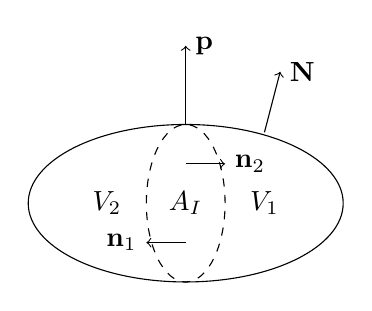
\begin{tikzpicture}
        \draw (0,0) ellipse (2 and 1);
        \draw[dashed] (0,0) ellipse (0.5 and 1)node{$A_I$};
        \draw[->](0,1)--++(0,1)node[right]{\textbf{p}}; 
        \draw[->](1,0.9)--++(0.2,0.77)node[right]{\textbf{N}}; 
        \draw[->](0,-0.5)--++(-0.5,0)node[left]{$\textbf{n}_1$}; 
        \draw[->](0,0.5)--++(0.5,0)node[right]{$\textbf{n}_2$}; 
        \draw (1,0)node{$V_1$};
        \draw (-1,0)node{$V_2$};
    \end{tikzpicture}
    \caption{Scheme of an arbitrary material control volume.   }
\end{figure}

Let $f^0$  be an arbitrary quantity to be conserved inside the non-material volume $\omega$. 
Then $\bm\Phi^0$ refer to the non-convective flux of $f^0$. 
Then $s^0$ refer to source term  related to  $f^0$. 
Then, for an arbitrary control volume we have, 
\begin{equation*}
    \ddt \int_{V} f^0 dV 
    = 
    \int_{V} s^0 dV 
    + \int_{\partial V} \mathbf{\Phi}^0 \cdot \textbf{N} dS,
\end{equation*}
where $\textbf{N}$ is the normal of the control volume. 
Any quantities defined in $V_k$ will be noted with a subscript $_k$ and those who are defined at the interface with $_I$. 
Therefore, if we decompose any quantity such as $f^0 = \sum_k f_k^0 \chi_k + f_I^0 \delta_I$ we obtain, 
\begin{multline*}
    \sum_k\left[\ddt \int_{V_k} f_k^0 dV 
    - \int_{V_k} s_k^0 dV 
    - \int_{A_k} \mathbf{\Phi}_k^0 \cdot \textbf{N} dS
    \right]
    + \ddt \int_{A_I} f_I^0 dS 
    - \int_{A_I} s_I^0 dS 
    - \int_{C} \mathbf{\Phi}_I^0 \cdot \textbf{p} dC 
    = 0
\end{multline*}
Using the Reynolds transport theorem on volume integral yields,
\begin{align*}
    \ddt \int_{V_k} f_k^0 dV 
    &= \int_{V_k} \pddt f_k^0 dV 
    + \int_{A_I \cup A_k} f_k^0 \textbf{u} \cdot \textbf{n}_k dS\\
    &= \int_{V_k} \left[
        \pddt f_k^0  + \div (f_k^0 \textbf{u}_k^0) 
    \right]dV 
    + \int_{A_I} f_k^0 (\textbf{u}_I^0 - \textbf{u}_k^0) \cdot \textbf{n}_k dS\\
\end{align*}
where $\textbf{n}_k$ is the normal of the interface $A_I$ on the outward direction of the $k$ phase. 

The second term is integrated only over $A_I$ as it is the interface between both phase and not the one of the control volume. 
Using the Ledbiz rule for integration on surface yields, 
\begin{align*}
    \ddt \int_{A_I} f_I^0 dS 
    &= \int_{A_I} \left[
        \pddt f_I^0  + \divI (f_I^0 \textbf{u}_I^0) 
    \right]dS
\end{align*}

Regarding the non-convective integrals, by using the divergence theorem we can write\citep{nadim1996concise}, 
\begin{align*}
    \int_{A_k} \mathbf{\Phi}_k^0\cdot \textbf{n}_k dS
    = \int_{V_k} \div\mathbf{\Phi}_k^0 dV
    - \int_{A_I} \mathbf{\Phi}_k^0\cdot \textbf{n}_k dS. 
\end{align*}
The last term can also be re-written with the divergence theorem \citet{nadim1996concise},
\begin{align*}
    \int_{C} \mathbf{\Phi}_I^0\cdot \textbf{p} dC 
    = \int_{A_I} \divI \mathbf{\Phi}_I^0 dS
    - \int_{A_I} \mathbf{\Phi}_I^0 \cdot \textbf{n} \div \textbf{n} dS
\end{align*}
Notice that whether it is $\textbf{n}_1$ or $\textbf{n}_2$ the second term on the left conserve the same sign. 

Taking in account these reformulations, we can re-write the integral balance previously exposed by, 
\begin{align*}
    \sum_k \int_{V_k}{\left[
        \pddt f_k^0
        + \div (f_k^0\textbf{u}_k^0 - \bm\Phi_k^0)
        - s_k^0
    \right]}\\
    + \sum_k\int_{A_I}{\left[
        f_k^0(\textbf{u}_I^0 - \textbf{u}_k^0)
        + \bm\Phi_k^0
    \right]\cdot \textbf{n}_k}
    + \int_{A_I}{\left[
        \pddt f_I^0 
        + \divI (f_I^0 \textbf{u}_I - \bm\Phi_I^0)
        + \bm\Phi_I^0 \cdot \textbf{n} \div \textbf{n}
    \right]} =0 
\end{align*}

Every integral of volume must be balanced independently of the surface integral. 
This means that we can separate this equation into two, 
\begin{equation*}
    \pddt f_k  
    + \div (f_k \textbf{u}_k - \mathbf{\Phi}_k) 
    =s_k. 
\end{equation*}
\begin{equation}
    \pddt f_I  
    + \divI (f_I \textbf{u}_I -\mathbf{\Phi}_I)
    + \mathbf{\Phi}_I \cdot \textbf{n} \div \textbf{n}
    = 
    + s_I
    - \sum_k \left[
    f_k (\textbf{u}_I - \textbf{u}_k)
    + \mathbf{\Phi}_k
    \right] \cdot \textbf{n}_k. 
    \label{ap:eq:dt_f_I}
\end{equation}
These equations are valid in $\Omega_k(t)$ and $\Sigma(t)$ for volume and surface quantity, respectively. 

Now let's reformulate the third term of the surface balance equation. 
Let $\textbf{F}$ be an arbitrary surface quantity. 
It can be split into two part such as, 
\begin{equation*}
    \textbf{F} 
    = \textbf{F} \cdot \textbf{n}\textbf{n}
    + (\textbf{I} - \textbf{nn})  \cdot \textbf{F}
    = \textbf{F}_\bot + \textbf{F}_{||}.
\end{equation*}
Injecting this decomposition inside the Gauss theorem on an arbitrary control volume it can be shown that, 
\begin{equation*}
    \int_{S} \divI \textbf{F}dS
    = 
    \int_{S} \left[\divI \textbf{F}_{||} 
    + \textbf{F} \cdot \textbf{n} \div\textbf{n}
    \right]dS
\end{equation*}
Consequently, we have the following relation,
\begin{equation*}
    \int_{A_I} \divI \bm\Phi_I^0dS
    = 
    \int_{A_I} \left[\divI \bm\Phi_{I||}^0
    + \bm\Phi_I^0 \cdot \textbf{n} \div\textbf{n}
    \right]dS
\end{equation*}

By taking in account this relation it is easy to take or not the normal components of a vector to the interface within the balance equaitons. 
For example, we can write either, 
\begin{equation}
    \pddt f_I  
    + \divI (f_I \textbf{u}^I_{||} -\mathbf{\Phi}^I_{||})
    + f_I \textbf{u}_I \cdot \textbf{n} \div \textbf{n}
    - s_I
    = 
    - \sum_k \left[
    f_k (\textbf{u}_I - \textbf{u}_k)
    + \mathbf{\Phi}_k
    \right] \cdot \textbf{n}_k 
    \label{ap:eq:dt_f_I2}
\end{equation}
Or 
\begin{equation}
    \pddt f_I  
    + \divI (f_I \textbf{u}^I -\mathbf{\Phi}^I_{||})
    - s_I
    = 
    - \sum_k \left[
    f_k (\textbf{u}_I - \textbf{u}_k)
    + \mathbf{\Phi}_k
    \right] \cdot \textbf{n}_k 
    \label{ap:eq:dt_f_I2}
\end{equation}
where we have changed the flux term formulation. 



\section{Topological equations}
There is two Topological equaitons one for $\chi_k$ and an other for $\delta_I$.
First, we recall the relations related to the phase indicator function, 
\begin{equation}
    \frac{\partial}{\partial t} \chi_k
    + \textbf{u}_I  \nablabh \chi_k 
    = 0, \;\;\;\;\text{and}\;\;\;\; 
    \nablabh \chi_k 
    = - \delta_I \textbf{n}_k.
    \label{ap:eq:phase_properties}
\end{equation}
Now the surface indicator function transport equation can be obtained using the Leibniz rule for differentiation,  
\begin{equation*}
    \ddt \int_{A_I} dS
    = \int_{A_I} \nablabh_I \cdot \textbf{u}_I dS,
\end{equation*}
Those integrals can be re rewritten as, 
\begin{equation*}
    \ddt \int_{V} \delta_I dV
    = \int_{V} \delta_I \nablabh_I \cdot \textbf{u}_I dV.
\end{equation*}
Then using the Reynolds transport term for fixed material volume yields,
\begin{equation*}
    \pddt \delta_I
    + \nablabh \cdot (\delta_I \textbf{u}_I)
    = \delta_I \nablabh_I \cdot \textbf{u}_I. 
\end{equation*}
This equation can also be takes the form 
\begin{equation}
    \pddt \delta_I
    + \nablabh \cdot (\delta_I \textbf{u}_I\cdot \textbf{n}\textbf{n})
    = \delta_I \textbf{u}_I \cdot \textbf{n}\nablabh \cdot \textbf{n}. 
    \label{ap:eq:dt_delta_I}
\end{equation}
Also, it can be useful to derive an expression for the gradient of the $\delta_I$ function. 
To do so we take the gradient of \ref{ap:eq:phase_properties} yielding, 
\begin{equation*}
    \nablabh\delta_I 
    = \nablabh( - \textbf{n}_k \cdot \nablabh \chi_k)
    = \nablabh\textbf{n}_k \cdot \textbf{n}_k \delta_I
    + \nablabh(\textbf{n}_k \delta_I) \cdot \textbf{n}_k 
\end{equation*}

\section{\textit{One-fluid} and \textit{two-fluid} formulations}
In this appendix we derive the \textit{two-fluid} and \textit{one-fluid} formulation of a generalized conservation equation, namely,
\begin{equation}
    \frac{\partial}{\partial t} f_k
    = \nablabh \cdot (\bm{\Phi}_k - f_k\textbf{u}_k)
    + \textbf{S}_k.
    \label{ap:eq:global_balance}
\end{equation}
Then we derive the phase averaged and global averaged equation of this general equation of conservation. 

We can derive the \textit{two-fluid} formulation by multiplying \ref{ap:eq:global_balance} by the phase indicator function \ref{eq:phase_indicator}. 
It yields, 
\begin{equation*}
    \frac{\partial}{\partial t} (\chi_k f_k)
    = \nablabh \cdot (\chi_k \bm{\Phi}_k - \chi_k f_k \textbf{u}_k)
    + \chi_k \textbf{S}_k.
    + f_k \frac{\partial}{\partial t} \chi_k
    + \left(
        f_k \textbf{u}_k 
        - \bm{\Phi}_k
    \right) \cdot \nablabh \chi_k
    % \label{ap:eq:global_balance}
\end{equation*}
where we have included the phase function $\chi_k$ into the derivative operators. 
Now, using the \ref{ap:eq:phase_properties} we get, 
\begin{equation}
    \frac{\partial}{\partial t} (\chi_k f_k)
    = \nablabh \cdot (\chi_k \bm{\Phi}_k - \chi_k f_k \textbf{u}_k)
    + \chi_k \textbf{S}_k
    + \left[
        \bm{\Phi}_k 
        + f_k 
        \left(
            \textbf{u}_I
            - \textbf{u}_k
        \right) 
    \right]
    \cdot \textbf{n}_k \delta_I 
    \label{ap:eq:two-fluid_global}
\end{equation}
where the last term is the interfacial source term, such as the drag force if $f_k$ is the momentum or the mass transfer if $f_k$ is the density. 
In this equation notice that all quantities are factor of the phase indicator function $\chi_k$. 
So we transport $\chi_k f_k$ which is field quantity defined over the whole domain. 
Thus, \ref{ap:eq:two-fluid_global} is valid over the entire domain.   

Now, we define the jump condition across the interface or the surface transport equation as the sum of the interfacial term on each phase $k$. 
It can be obtained using  the transport of surface \ref{ap:eq:dt_f_I2}.
Indeed, multiplying \ref{ap:eq:dt_f_I2} by $\delta_I$ gives, 
\begin{equation}
    \pddt (f_I\delta_I)  
    = 
    + \nablabh \cdot (\delta_I \mathbf{\Phi}^I_{||} - \delta_I f_I \textbf{u}^I)
    +\textbf{S}_I \delta_I
    - \sum_k \left[
    f_k (\textbf{u}_I - \textbf{u}_k)
    + \mathbf{\Phi}_k
    \right] \cdot \textbf{n}_k \delta_I
    \label{ap:eq:general_jump}
\end{equation}
\tb{
    Notice that the first term on the RHS is the parallele component of $\mathbf{\Phi}$ thus it must be reformulated as, 
    
}

Now, let's derive the \textit{one-fluid} formulation of the general conservation law.
To do so we sum on all phases \ref{ap:eq:two-fluid_global} plus the interface. 
Besides, we define any quantities $q$ such as, $q = \sum_k \chi_k q_k + \delta_I q_I$.
Then it is trivial to show that, 
\begin{equation}
    \frac{\partial}{\partial t} f
    = \nablabh \cdot (\bm{\Phi} - f \textbf{u})
    + \textbf{S}
    \label{ap:eq:one-fluid_global}
\end{equation}
which is the \textit{one-fluid} formulation. 

The volume average of \ref{ap:eq:two-fluid_global} is then straight forward, by using the definition of the averaged operator, we get, 
\begin{equation*}
    \frac{\partial}{\partial t} (\phi_k\kavg{f})
    = \nablabh \cdot \left(
        \phi_k \kavg{\bm{\Phi} - f \textbf{u}}
    \right)
    + \phi_k \kavg{\textbf{S}}
    + a_I \Iavg{
        \bm{\Phi}_k \cdot \textbf{n}_k
        + f_k 
        \left(
            \textbf{u}_I
            - \textbf{u}_k
        \right) \cdot \textbf{n}_k
    } 
\end{equation*}
Similarly, the bulk average can be obtained by averaging \ref{ap:eq:one-fluid_global} yielding, 
\begin{equation*}
    \frac{\partial}{\partial t} \avg{f}
    = \nablabh \cdot \avg{\bm{\Phi} - f \textbf{u}}
    + \avg{\textbf{S}}
    % + a_I\avg{\textbf{J}_I},
    \label{ap:eq:avg_global}
\end{equation*}
\section{Derivation of the point velocity}
Consider a particle of center of mass $\textbf{y}_\alpha$ defined such as
\begin{equation*}
    m_\alpha \textbf{y}_\alpha
    = \int_{V_\alpha} \rho_k \textbf{y}_k dV,
\end{equation*}
its velocity can be solely the derivation of $\textbf{y}_\alpha$ whitin time.
Yielding, 
\begin{align*}
    \ddt \textbf{y}_\alpha (t)
    &=
    \ddt \left(
        \frac{1}{m_\alpha} \int_{V_\alpha} \rho_k \textbf{y}_k dV
    \right)\\
    &= \frac{1}{m_\alpha}
    \ddt 
    \left(
        \int_{V_\alpha} \rho_k \textbf{y} dV
    \right)
    - \frac{1}{m_\alpha^2} \ddt \int_{V_\alpha} \rho_k dV \int_{V_\alpha} \rho_k \textbf{y}_k dV
    \\
    &= \frac{1}{m_\alpha}\int_{V_\alpha} \left[
        \pddt (\rho_k \textbf{y}) + \nablabh \cdot\left(\rho_k \textbf{y}\textbf{u}_k\right) dV 
    \right]\\
    &+ \frac{1}{m_\alpha}\int_{S_\alpha} \textbf{y} M_k d S
    -  \frac{1}{m_\alpha^2} \int_{S_\alpha} M_k dS  \int_{V_\alpha} \rho_k \textbf{y}_k dV
    \\
    &= \frac{1}{m_\alpha}\int_{V_\alpha} \textbf{y} \left[
    \pddt (\rho_k) + \nablabh \cdot\left(\rho_k \textbf{u}_k\right) dV 
    \right]dV
    + \frac{1}{m_\alpha}\int_{V_\alpha} \rho_k  \textbf{u}_k  \cdot \nablabh \textbf{y} dV \\
    &+ \frac{1}{m_\alpha}\int_{S_\alpha} \textbf{y}_k M_k d S
    - \frac{1}{m_\alpha}  \textbf{y}_\alpha \int_{S_\alpha} M_k dS
\end{align*}
By considering the mass conservation \ref{eq:single-fluid_mass} for the first term,  noticing that $\nablabh \textbf{y} = \textbf{I}$ where $\textbf{I}$ is the identity tensor for the second term and introducing \textbf{r} in the third term gives, we get the following relation,
\begin{equation*}
    \textbf{u}_\alpha
    = \frac{1}{m_\alpha} \left(
        \textbf{p}_\alpha
        +  \int_{S_\alpha} \textbf{r} M_k dS
    \right)
    % = \frac{1}{m_\alpha}  \left(
    %     \textbf{p}_\alpha
    % - \int_{V_\alpha} \rho_k \textbf{w} dV
    % \right)
\end{equation*}

\section{Derivation of the surface transport equations for Lagrangian particles}

By making use of the Leibniz rule together with \ref{ap:eq:dt_f_I} it can be shown that for any surface quantity $f_I$ we have, 
\begin{align*}
    \ddt \int_{S_\alpha} f_I dS
    &= \int_{S_\alpha} \pddt f_I 
    + \nablabh_I \cdot (\textbf{u}_If_I) dS\\
    &= \int_{S_\alpha} \left(
        \nablabh_I \cdot \mathbf{\Phi}_{||}^I
        + \textbf{S}_I
    \right) dS\\
    & - \sum_k \int_{S_\alpha} \left[
        f_k (\textbf{u}_I - \textbf{u}_k)
        + \mathbf{\Phi}_k
    \right] \cdot \textbf{n}_k
    dS
\end{align*}
Then remark that if $\mathbf{\Phi} = \sigma (\textbf{I}-\textbf{nn})$.
Then, 
\begin{equation*}
    \int_S \nablabh_I \cdot \left[\sigma (\textbf{I} - \textbf{nn})\right]dS 
    =
    \int_S  \nablabh_I \sigma dS 
    + \int_S \sigma \kappa \textbf{n}dS 
    = 0
\end{equation*}

Using the Gauss theorem for closed surface it can be shown easily that the first term on the RHS can be reformulated, leaving with, 
\begin{align}
    \ddt \int_{S_\alpha} f_I dS
    = \int_{S_\alpha} \left[
        \textbf{S}_I 
        - \kappa \mathbf{\Phi}_{||}^I\cdot \textbf{n} 
    \right]dS
    - \sum_k \int_{S_\alpha} \left[
        f_k (\textbf{u}_I - \textbf{u}_k)
        + \mathbf{\Phi}_k
    \right] \cdot \textbf{n}_k
    dS
\end{align}
In this equation we can see that $\mathbf{\Phi}_I$ plays no role at all. 

Now let's derive the first moment of a surface quantity, namely $f_I \textbf{r}$. 
\begin{align*}
    \ddt \int_{S_\alpha} f_I \textbf{r} dS
    &= \int_{S_\alpha} \textbf{r}\left[
        \pddt f_I 
        + \nablabh_I \cdot (\textbf{u}_If_I) 
    \right]dS
    + \int_{S_\alpha}
    f_I \left[
        \pddt \textbf{r} + \textbf{u}_I \cdot \nablabh_I \textbf{r}
    \right]
    dS\\
\end{align*}
Using \ref{ap:eq:dt_f_I} on the first term of the RHS and the relation $\nablabh_I \textbf{r} = (\textbf{I} - \textbf{nn})$ gives, 
\begin{align*}
    \ddt \int_{S_\alpha} f_I \textbf{r} dS
    &= \int_{S_\alpha} \textbf{r}\left[
        \nablabh_I \cdot \mathbf{\Phi}_I
        - \Phi_I\cdot\textbf{n}\nablabh\textbf{n}
        + \textbf{S}_I
    \right] dS\\
    & - \sum_k \int_{S_\alpha}\textbf{r} \left[
        f_k (\textbf{u}_I - \textbf{u}_k)
        + \mathbf{\Phi}_k
    \right] \cdot \textbf{n}_k
    dS\\
    &+ \int_{S_\alpha}
    f_I (\textbf{u}^I_{||} - \textbf{u}_\alpha)
    dS\\
\end{align*}
Using the Gauss theorem for closed surface on the first term on the RHS, this equation can be simplified to, 
\begin{align}
    \ddt \int_{S_\alpha} f_I \textbf{r} dS
    &= \int_{S_\alpha} \left(
        \textbf{S}_I\textbf{r}
        - \mathbf{\Phi}_{||}^I
    \right) dS
    + \int_{S_\alpha}
    f_I \textbf{w}_I
    dS\nonumber\\
    & - \sum_k \int_{S_\alpha}\textbf{r} \left[
        f_k (\textbf{u}_I - \textbf{u}_k)
        + \mathbf{\Phi}_k
    \right] \cdot \textbf{n}_k
    dS
    \label{ap:eq:dt_r_f_I}
\end{align}
where $\textbf{w}_{I||} = \textbf{u}_{I||} - \textbf{u}_\alpha$. 
In the jump condition of the first moment it is now evident that $\mathbf{\Phi}^I_{||}$ is relevant. 

As an example, if $f_I$ were to be the momentum of the surface, then $\mathbf{\Phi}_{||}^I = \sigma (\textbf{I} - \textbf{nn})$. 
Thus, we can express the integrals as, 
\begin{equation*}
    \int_{S_\alpha}\mathbf{\Phi}_{||}^IdS
    =\int_{S_\alpha} \sigma (\textbf{I} - \textbf{nn}) dS
    =\int_{S_\alpha} \nablabh_I \cdot (\sigma \textbf{r}) dS
    =\int_{S_\alpha} \sigma \textbf{r} (\nablabh\cdot\textbf{n}) \textbf{n} dS
\end{equation*} 
where we used the Gauss theorem on closed surface for the first term. 
In this last expression we recognize the last term as begin the first moment of the surface tension force. 




\section{Decomposition of the particular energy balance.}
This section is a detailed derivation of the energy equation for a whole fluid particle, namely,
\begin{equation*}
    \label{ap:eq:E_alpha_dt}
    \ddt E_\alpha 
    % = \ddt \int_{V_\alpha} \rho_k E_k dV
    = \int_{V_\alpha} \textbf{b}_k \cdot \textbf{u}_k dV
    + \int_{S_\alpha} \left[
        (\textbf{T}\cdot \textbf{u} 
    - \textbf{q})\cdot\textbf{n}_k 
    + M_k E_k 
    + \textbf{f}_I \cdot \textbf{u}_I 
    \right]dS, 
\end{equation*}
Since we can decompose the velocity fields of a particle following $\textbf{u}_k = \textbf{u}_\alpha + \textbf{w}$ it is then possible to rewrite the total energy, 
Yielding, 
\begin{multline*}
    \int_{V_\alpha} \rho_k E_k dV
    = \int_{V_\alpha} \rho_k e_k dV
    + \frac{1}{2} \int_{V_\alpha} \rho_k \textbf{u}_\alpha\cdot\textbf{u}_\alpha dV\\
    + \int_{V_\alpha} \rho_k \textbf{u}_\alpha\cdot\textbf{w} dV
    + \frac{1}{2} \int_{V_\alpha} \rho_k \textbf{w}\cdot\textbf{w} dV
\end{multline*}
by applying the relation \ref{eq:M_alpha_dt} on the second term, it is possible to show that,
\begin{equation*}
    E_\alpha
    = \int_{V_\alpha} \rho_k e_k dV
    + \frac{1}{2} \textbf{u}_\alpha\cdot\textbf{u}_\alpha  m_\alpha
    + \textbf{u}_\alpha\cdot \int_{V_\alpha} \rho_k \textbf{w} dV
    + \frac{1}{2} \int_{V_\alpha} \rho_k \textbf{w}\cdot\textbf{w} dV.
\end{equation*}
We clearly see that the energy can be decomposed into internal and kinetic energy. 
We define the integrated internal energy of the particle by $e_\alpha = \int_{V_\alpha} = \rho_k e_k dV$.
It is the straight forward (using \ref{eq:one-fuild_internal_energy}) to show that, 
\begin{equation*}
    \ddt e_\alpha
    = \int_{V_\alpha} \textbf{T}:\nablabh\textbf{u}_k dV
    + \int_{S_\alpha} \left(
        e_k M_k
        - \textbf{q}_k \cdot \textbf{n}_k
    \right) dS.
\end{equation*}
Similarly, the kinetic energy equation for a whole fluid particle can be obtained deriving the local kinetic energy ,namely,
\begin{equation*}
    \ddt \int_{V_\alpha} \rho_k \frac{u_k^2}{2} dV
    = \int_{V_\alpha}\textbf{u}_k \cdot  \left(
        \textbf{b}_k
        + \nablabh \cdot \textbf{T}_k
    \right)dV
    + \int_{S_\alpha} \frac{u_k^2}{2} M_k dS.
\end{equation*}
Using the velocity decomposition one can deduce, 
\begin{multline}
    \frac{1}{2} \ddt \left(
        m_\alpha \textbf{u}_\alpha \cdot \textbf{u}_\alpha
        + 2\textbf{u}_\alpha \cdot \int_{V_\alpha}  \rho_k \textbf{w}_k dV
        + \int_{V_\alpha} \rho_k \textbf{w}_k \cdot \textbf{w}_k dV
    \right)\\
    =  \textbf{u}_\alpha \left[
        \cdot\int_{V_\alpha} \textbf{b}_k dV
        +  \int_{S_\alpha} \left(
            \textbf{T}_k \cdot \textbf{n}_k
            + \frac{1}{2} \textbf{u}_\alpha M_k 
            + \textbf{w}_k M_k 
        \right)dS
    \right]\\
    + \int_{V_\alpha} \left(
        \textbf{w}_k\cdot\textbf{b}_k
        -\textbf{T}_k : \nablabh \textbf{w}_k
    \right)dV
    + \int_{S_\alpha} 
        \textbf{w}_k\cdot(\textbf{T}_k\cdot \textbf{n}_k)
    dS\\
    + \int_{S_\alpha} \frac{1}{2} \textbf{w}_k \cdot \textbf{w}_k M_k dS.
    \label{ap:eq:u_2_dt}
\end{multline}
Besides, taking the dot product of the centered velocity $\textbf{u}_\alpha$, with the momentum equation \ref{eq:dt_p_alpha}, gives, 
\begin{multline*}
    \frac{1}{2}\ddt (m_\alpha \textbf{u}_\alpha \cdot \textbf{u}_\alpha)
    + \textbf{u}_\alpha \cdot \ddt \int_{V_\alpha} \rho_k \textbf{w}_k dV \\
    = \textbf{u}_\alpha \cdot \int_{V_\alpha} \textbf{b}_k dV
    + \textbf{u}_\alpha \cdot \int_{S_\alpha} \left(
    \textbf{T}_k \cdot\textbf{n}_k
    +\frac{\textbf{u}_\alpha}{2} M_k
    +\textbf{w}_k M_k
    \right)dS,
\end{multline*}
We can notice that the RHS of this equation correspond rigorously to the second line of \ref{ap:eq:u_2_dt}.
Therefore, taking the difference between those equations, yields the internal motion equation of an arbitrary particle, namely, 
\begin{multline*}
    \frac{1}{2}\ddt \int_{V_\alpha} \frac{\rho_k}{2} \textbf{w}_k \cdot \textbf{w}_k dV
    = \int_{V_\alpha} \left(
        \textbf{w}_k\cdot\textbf{b}_k
        -\textbf{T}_k : \nablabh \textbf{w}_k
    \right)dV\\
    + \int_{S_\alpha} 
        \textbf{w}_k\cdot(\textbf{T}_k\cdot \textbf{n}_k)
    dS
    + \int_{S_\alpha} \frac{1}{2} \textbf{w}_k \cdot \textbf{w}_k M_k dS.
\end{multline*}

\section{Derivation of kinetic Turbulence Evolution Equations}

The aim of this section is to derive the transport equation for the granular temperature scalar. 
Let's define the grain temperature, $T$ as such, $T =\frac{1}{2} \textbf{u}'\cdot\textbf{u}'$, where $\textbf{u}'$ is the fluctuation velocity of a given average procedure. 

\subsection{For a continuous phase}
We start this derivation for the continuous phase $k$, so that $\textbf{u}'_k = \textbf{u}_k - \kavg{\textbf{u}}$.
We start from the averaged kinetic energy equation over the $k$ phase, namely : 
\begin{multline*}
    \frac{\rho_k}{2}\frac{\partial }{\partial t}\left(
        \phi_k
        \kavg{u^2}
    \right)
    +\frac{\rho_k}{2}\nablab\cdot \left(
        \phi_k
        \kavg{u^2\textbf{u}}
    \right)
    =
    \nablab\cdot\left(
        \phi_k
        \kavg{\textbf{u}\cdot \textbf{T}}
    \right)
    +\phi_k\kavg{\textbf{u}\cdot\textbf{b} - \textbf{T}: \nablabh\textbf{u}}\\
    +a_I \Iavg{
        (\textbf{T}_k\cdot\textbf{u}_k)\cdot\textbf{n}_k
        + \frac{u^2_k}{2} M_k}.
\end{multline*}
Breaking down the LHS of this equation times $\frac{2}{\rho_k}$, yields,
\begin{align*}
    &\frac{\partial }{\partial t}\left(
        \phi_k
        \kavg{u^2}
    \right)
    +
    \nablab\cdot \left(
        \phi_k
        \kavg{u^2\textbf{u}}
    \right)\\
    &=
    \phi_k\frac{\partial }{\partial t}\kavg{u^2}
    +\kavg{u^2}\frac{\partial }{\partial t}\phi_k
    +\nablab\cdot \left(
        \phi_k
        \kavg{u^2}\kavg{\textbf{u}}
        +\phi_k
        \kavg{u^2\textbf{u}'}
    \right)\\
    &=
    \phi_k
    \left[
        \frac{\partial }{\partial t}\kavg{u^2}
        + 
        \kavg{\textbf{u}}
        \cdot\nablab 
        \kavg{u^2}
    \right]
    +\kavg{u^2} \left[
        \frac{\partial }{\partial t}\phi_k
        + \nablab\cdot \left(
            \phi_k
            \kavg{\textbf{u}}
        \right)
    \right]\\
    &+ \nablab\cdot \left(
        2\phi_k
        \kavg{\textbf{u}}\cdot\kavg{\textbf{u'}\textbf{u'}} + \phi_k \kavg{T \textbf{u'}}
    \right)
\end{align*}
where we used $\kavg{u^2} = \kavg{u}^2 + T$. 
By using the averaged mass conservation \ref{eq:avg_k_mass} times $\frac{1}{2}\kavg{u^2}$, namely, 
\begin{equation*}
    \frac{\rho_k}{2} \kavg{u^2} \pddt \phi_k 
    + \frac{\rho_k}{2} \kavg{u^2} \nablab \cdot\left(\phi_k\kavg{\textbf{u}}\right)
    = \frac{a_I}{2}\kavg{u^2}\Iavg{M_k},
\end{equation*}
we can rewrite the energy balance in conservative form. 
It reads as, 
\begin{multline}
    \phi_k\frac{\rho_k}{2}  \left[
        \frac{\partial }{\partial t}
        \kavg{u^2}
        +\kavg{\textbf{u}}\cdot\nablab 
        \kavg{u^2}
    \right]
    =
    \nablab\cdot\left(
        \phi_k
        \kavg{\textbf{u}\cdot \textbf{T}
        - \rho_k\kavg{\textbf{u}}\cdot\textbf{u'u'}
        - \frac{\rho_k}{2}T\textbf{u'}}
    \right)\\
    +\phi_k\kavg{\textbf{u}\cdot\textbf{b} - \textbf{T}: \nablabh\textbf{u}}
    +a_I \Iavg{
        (\textbf{T}_k\cdot\textbf{u}_k)\cdot\textbf{n}_k
        + \frac{u^2_k - \kavg{u^2}}{2} M_k}.
    \label{ap:eq:avg_k_u_2}
\end{multline}
On the other hand the momentum equation reads as, 
\begin{multline*}
    \rho_k\pddt (\phi_k\kavg{\textbf{u}}) 
    + \rho_k\nablab\cdot(\phi_k\kavg{\textbf{u}}\kavg{\textbf{u}})\\
    = \nablab\cdot\left[
        \phi_k \kavg{\textbf{T}
        - \rho_k \textbf{u'u'}}
    \right]
    +\phi_k\kavg{\textbf{b}}
    + a_I\Iavg{M_k \textbf{u}_k +\textbf{n}_k\cdot\textbf{T}_k},
\end{multline*}
using the mass balance times $\kavg{\textbf{u}}$, we can write the momentum equation as, 
\begin{multline*}
    \rho_k \phi_k \left[
        \pddt \kavg{\textbf{u}}
        + \kavg{\textbf{u}}\cdot\nablab\kavg{\textbf{u}}
    \right]\\
    = \nablab\cdot\left[
        \phi_k \kavg{\textbf{T}
        - \rho_k \textbf{u'u'}}
    \right]
    +\phi_k\kavg{\textbf{b}}
    + a_I\Iavg{M_k \left(\textbf{u}_k - \kavg{\textbf{u}}\right) +\textbf{n}_k\cdot\textbf{T}_k}.
\end{multline*}
Then taking the dot product of this equation with $\kavg{\textbf{u}}$ gives, 
\begin{multline}
    \phi_k\frac{\rho_k}{2}  \left[
        \pddt \kavg{u}^2
        + \kavg{\textbf{u}}\cdot\nablab\kavg{u}^2
    \right]\\
    = \nablab\cdot\left[
        \phi_k \kavg{\textbf{u}}\cdot\kavg{\textbf{T}
        - \rho_k  \textbf{u'u'}}
    \right]
    +\phi_k\kavg{\rho_k \textbf{u'u'} - \textbf{T}}:\nablab
         \kavg{\textbf{u}}\\
    +\phi_k\kavg{\textbf{u}}\cdot\kavg{\textbf{b}}
    + a_I\Iavg{M_k \left(\textbf{u}_k\cdot\kavg{\textbf{u}} 
    - \kavg{u}^2\right) +\textbf{n}_k\cdot(\kavg{\textbf{u}}\cdot\textbf{T}_k)}.
    \label{ap:eq:avg_k_u_u}
\end{multline}
Finally, we can obtain the transport equation of $T$ by subtracting \ref{ap:eq:avg_k_u_2} with \ref{ap:eq:avg_k_u_u}. 
Yielding the following equation, 
\begin{multline}
    \phi_k\rho_k  \left[
        \frac{\partial }{\partial t}
        \kavg{T}
        +\kavg{\textbf{u}}\cdot\nablab 
        \kavg{T}
    \right]\\
    =
    \nablab\cdot\left(
        \phi_k
        \kavg{\textbf{u'}\cdot \textbf{T'}
        - \rho_k T\textbf{u'}}
    \right)
    +\phi_k\kavg{\rho_k \textbf{u'u'}}:\nablab
         \kavg{\textbf{u}}\\
    +\phi_k\kavg{\textbf{u'}\cdot\textbf{b'} + \textbf{T'}: (\nablabh\textbf{u})'}
    +a_I \Iavg{
        (\textbf{T}_k'\cdot\textbf{u}'_k)\cdot\textbf{n}_k
        + T M_k}.
    \label{ap:eq:avg_k_T}
\end{multline}


\subsection*{Dispersed phase}

In the same spirit as the previous section we carry out the derivation for the transport of the kinetic turbulence evolution $T$. 
The only difference is that $T$ is now defined relative to the mean velocity of the particular phase $\pavg{u}$.  
From the previous section we know that we can write the energy equation under the following form, 
\begin{multline*}
    \frac{1}{2}\ddt (m_\alpha u^2_\alpha)
    + \textbf{u}_\alpha \cdot \ddt \int_{V_\alpha} \rho_k \textbf{w}_k dV 
    = \textbf{u}_\alpha \cdot \int_{V_\alpha} \textbf{b}_k dV\\
    + \textbf{u}_\alpha \cdot \int_{S_\alpha} \left[
    \textbf{T}_k \cdot\textbf{n}_k
    +\frac{\textbf{u}_\alpha}{2} M_k
    +\textbf{w}_k M_k
    \right]dS.
\end{multline*}
Applying the particular average operator yields the averaged point of mass kinetic energy equation, 
\begin{multline*}
    \frac{1}{2}\pddt   \left(\pavg{m_\alpha} \pnavg{u^2_\alpha}\right)
    + \frac{1}{2}\nablab \cdot \left(\pavg{m_\alpha} \pnavg{u^2_\alpha \textbf{u}_\alpha}\right) 
    = \pavg{\textbf{u}_\alpha \cdot \int_{V_\alpha} \textbf{b}_k dV}\\
    - \frac{1}{2}\pddt \left(\pavg{m_\alpha'(u_\alpha^2)'}\right)
    - \frac{1}{2}\nablab\cdot\left(\pavg{m_\alpha' (u_\alpha^2 \textbf{u}_\alpha)'}\right)\\
    - \pavg{\textbf{u}_\alpha \cdot \ddt \int_{V_\alpha} \rho_k \textbf{w}_k dV} 
    + \pavg{\textbf{u}_\alpha \cdot \int_{S_\alpha} \left[
    \textbf{T}_k \cdot\textbf{n}_k
    +\frac{\textbf{u}_\alpha}{2} M_k
    +\textbf{w}_k M_k
    \right]dS}.
\end{multline*}
From this step, we can carry out the same decomposition as the previous section for the RHS/2. 
Namely, 
\begin{multline*}
    \frac{\partial }{\partial t}\left(
        \pavg{m_\alpha}
        \pnavg{u^2_\alpha}
    \right)+
    \nablab\cdot \left(
        \pavg{m_\alpha}
        \pnavg{u^2_\alpha\textbf{u}_\alpha}
    \right) \\
    =
    \pavg{m_\alpha}
    \left[
        \frac{\partial }{\partial t}\pnavg{u^2_\alpha}
        + 
        \pnavg{\textbf{u}_\alpha}
        \cdot\nablab 
        \pnavg{u^2_\alpha}
    \right]
    +\pnavg{u^2_\alpha} \left[
        \frac{\partial }{\partial t}\pavg{m_\alpha}
        + \nablab\cdot \left(
            \pavg{m_\alpha}
            \pnavg{\textbf{u}_\alpha}
        \right)
    \right]\\
    + \nablab\cdot \left(
        2\pavg{m_\alpha}
        \pnavg{\textbf{u}_\alpha}\cdot\pnavg{\textbf{u'}\textbf{u'}} 
        + \pavg{m_\alpha} \pnavg{T \textbf{u'}}
    \right)
\end{multline*}
As we can observe the possible polydispersity of the flow, add supplementary terms linked to the fluctuation of the mass, $m_\alpha'$.
The energy equations in the conservative form then reads as, 
\begin{multline*}
    \frac{\pavg{m_\alpha}}{2}
    \left[
        \frac{\partial }{\partial t}\pnavg{u^2_\alpha}
        + 
        \pnavg{\textbf{u}_\alpha}
        \cdot\nablab 
        \pnavg{u^2_\alpha}
    \right]
    = \pavg{\textbf{u}_\alpha \cdot \int_{V_\alpha} \textbf{b}_k dV} + \nablab \cdot \textbf{L}\\
    - \pavg{\textbf{u}_\alpha \cdot \ddt \int_{V_\alpha} \rho_k \textbf{w}_k dV} 
    - \pavg{u_\alpha^2}\pnavg{\int_{S_\alpha} M_k d S}\\
    + \pavg{\textbf{u}_\alpha \cdot \int_{S_\alpha} \left[
    \textbf{T}_k \cdot\textbf{n}_k
    +\frac{\textbf{u}_\alpha}{2} M_k
    +\textbf{w}_k M_k
    \right]dS},
\end{multline*}
where \textbf{L} represent all the fluctuation terms derived in the two previous equations. 

Now let's look at the particular averaged momentum equation. 
Using similar decomposition as in the previous part,
and by using the decomposition of the momentum, $\textbf{p}_\alpha = m_\alpha \textbf{u}_\alpha + \int_{V_\alpha} \textbf{w}_k dV$, the equation aforesaid reads as, 
\begin{multline*}
    \pavg{m_\alpha} \left[
        \pddt \pnavg{\textbf{u}_\alpha}
        + \pnavg{\textbf{u}_\alpha}\cdot\nablab\pnavg{\textbf{u}_\alpha}
    \right]
    = \pavg{\int_{V_\alpha} \textbf{b}_k dV}
    + \nablab \cdot \textbf{R}\\
    - \pavg{\ddt \int_{V_\alpha} \rho_k \textbf{w}_k dV} 
    + \pavg{\int_{S_\alpha} \left[\textbf{T}_k + \rho_k \textbf{u}_k (\textbf{u}_I-\textbf{u}_k) \right] \cdot \textbf{n}_k d S}
\end{multline*}
where \textbf{R} is the term that gather all the fluctuation terms. 
Multiplying, this equation by $\pnavg{\textbf{u}_\alpha}$ and taking the difference with the energy equation yielding, 
\begin{multline*}
    \frac{\pavg{m_\alpha}}{2}
    \left[
        \frac{\partial }{\partial t}\pnavg{T_\alpha}
        + 
        \pnavg{\textbf{u}_\alpha}
        \cdot\nablab 
        \pnavg{T_\alpha}
    \right]
    = \pavg{\textbf{u}_\alpha' \cdot \left(\int_{V_\alpha} \textbf{b}_k dV\right)'} 
    + \nablab \cdot \left(\textbf{L}-\textbf{R}\right)\\
    - \pavg{\textbf{u}_\alpha' \cdot \left(\ddt \int_{V_\alpha} \rho_k \textbf{w}_k dV\right)'} \\
    - \pavg{T_\alpha}\pnavg{\int_{S_\alpha} M_k d S}
    + \pavg{\textbf{u}_\alpha \cdot \int_{S_\alpha} \left[
    \textbf{T}_k \cdot\textbf{n}_k
    +\frac{\textbf{u}_\alpha}{2} M_k
    +\textbf{w}_k M_k
    \right]dS},
\end{multline*}
% \chapter{Equivalence between volume average and weighted average for Lagrangian poly-disperse particles}
\label{ap:equivalence}
As mentioned in \ref{chap:avg} the velocity fields $\left<\bm{u}\right>^L_\gamma$ is needed in \ref{eq:PBM_QBMM}.
While, with the particular-average, \ref{eq:classic_hybrid_momentum_c}, we solve for $\left<\bm{u}\right>^p$.
Also, in \ref{eq:classic_hybrid_momentum_c} we have assumed an even distribution of particles size where this is clearly not the case. 
In the following we show the equivalence between the two averaged quantities and the correctness of the uniformity assumption. 
This appendix aim to prove rigorously the link between the population balance model and the particular-average equation.
The strategy is to derive \ref{eq:classic_hybrid_momentum_p} from Liouville equation following the method of \citet{curtiss1956kinetic} and \citet[chapter~7]{rao2008introduction}.
This way we show an equivalence by identification between the quantities mentioned above.

Let's consider the Boltzmann equation for a distribution $P(\textbf{x},\mathscr{C})$.
The distribution must remain physical, thus it must respect $\lim_{\mathscr{C} \rightarrow \partial\mathscr{C}} = 0$, where $\partial \mathscr{C}$ correspond to the boundary of the domain of definition of each component of $\mathscr{C}$. 
It yields, 
\begin{equation}
    \label{eq:Liouville}
    \pddt P(\textbf{x},\mathscr{C})
    + \bm{\nabla} \cdot \left(\textbf{u} P(\textbf{x},\mathscr{C})\right)
    + \grad_\mathscr{C} \cdot \left(\frac{d\mathscr{C}}{dt} P(\textbf{x},\mathscr{C})\right) 
    = \Psi
\end{equation}
Now let's consider a function $f(\mathscr{C},t)$ which represent any physical quantity function of the internal coordinate and the time. 
Multiplying \ref{eq:Liouville} by the function, $q_\alpha$, and integrating over all the internal coordinates yields Maxwell equation,
\begin{equation}
    \int q_\alpha \pddt P d\mathscr{C}
    + \int q_\alpha \grad \cdot \left(\textbf{u} P\right)d\mathscr{C}
    + \int q_\alpha \grad_\mathscr{C} \cdot \left(\frac{d\mathscr{C}}{dt} P\right) d\mathscr{C} = \int q_\alpha \Psi d\mathscr{C}.
\end{equation}
The first two terms derivative can be swapped with the integral since they are not function of $\mathscr{C}$.
Then, we make use of the divergence theorem on the third term, 
yielding,
\begin{multline}
    \pddt \int q_\alpha  P d\mathscr{C}
    + \grad \cdot\int q_\alpha \left(\textbf{u} P\right)d\mathscr{C} 
    % + \int_{\partial \lambda} \grad_\mathscr{C} \cdot \left(f \textbf{u}_\lambda P\right) d\partial\mathscr{C} 
    = \int q_\alpha \Psi d\mathscr{C},
    +\int \left(\frac{d\mathscr{C}}{dt} P\right) \cdot \grad_\mathscr{C} f  d\mathscr{C} 
    \label{eq:inttt}
\end{multline}
The second integral on RHS has been derived using the divergence theorem and considering that the distributions $P$ vanish near its boundaries. 
After applying the average operator \ref{eq:inttt} reads as,
\begin{equation}
    \pddt \left( n \avg{q_\alpha}\right)
    + \bm{\nabla} \cdot \left(n \avg{\textbf{u} q_\alpha}\right)
    = n \avg{\Psi q_\alpha}
    + n  \avg{\frac{d\mathscr{C}}{dt} \cdot \grad_\mathscr{C} q_\alpha}
    \label{ap:eq:maxwell}
\end{equation}
Note that up to now we have made no assumption on the shape of $P$ and on the nature of the internal coordinates $\mathscr{C}$. 
Nevertheless, only the number of particles  $n$, appear in \ref{ap:eq:maxwell}.
At this point of the development we must specify the nature of the internal coordinates.
Thus, in the next section we investigate different situation. 
In this context the scalar $\Psi$ represent the source term due to 3 things. 
The coalescence and break-up phenomena, and the inter particular collision. 
The source term can be thus expressed under this form \citep{rao2008introduction,curtiss1956kinetic},  
\begin{equation*}
    \Psi(\mathscr{C}) = B(\mathscr{C}) + D(\mathscr{C}) + \Pi(\mathscr{C}) + \nabla \cdot \Theta(\mathscr{C})
\end{equation*}
where $B$ is the birth term, $D$ the death term, $\Pi$ the collision source term, and $\Theta$ the collision flux. 

\section{Point mass particles}
We start by considering only point of mass particles. 
Therefore, we consider only the momentum of the particles $\textbf{p}_\alpha$ and the volume $V_\alpha$ as an internal coordinate.
Thus, \ref{ap:eq:maxwell} yields,
\begin{equation}
    \pddt \left( n \avg{q_\alpha}\right)
    + \bm{\nabla} \cdot \left(n \avg{q_\alpha \textbf{u}_\alpha}\right)
    - n  \avg{\frac{\partial V_\alpha}{\partial t} \cdot \frac{\partial q_\alpha}{\partial V_\alpha}}
    - n  \avg{\frac{\partial \textbf{p}_\alpha}{\partial t} \cdot \frac{\partial q_\alpha}{\partial \textbf{p}_\alpha}}
    = n \avg{\Psi q_\alpha},
\end{equation}
From this equation we can recover the conservation equations of the particular phase by replacing $q_\alpha$ by the right quantity. 
Consider, $f = 1$, for example, we get, 
\begin{equation}
    \pddt n
    + \grad \cdot \left(n \avg{\textbf{u}_\alpha}\right)
    = n\avg{\Psi}
\end{equation}
which is the conservation of the number density of the particles. 
Where the right-hand side is to coalesce and break up kernel.
Similarly, the mass balance equation can be obtained with $f = V_\alpha \rho_d$, yielding,
\begin{equation}
    \pddt (n\avg{m_\alpha})
    + \bm{\nabla} \cdot \left(n \avg{\textbf{u}_\alpha m_\alpha}\right)
    =
    n  \avg{\int_{S_\alpha} M_d dS},
\end{equation}
where we have use \ref{eq:dt_m_alpha} to make appear the mass transfer term. 
Note that the source term is null since coalescence and break-up conserve the mass. 
Again, for the momentum conservation equation we set $f = \textbf{p}_\alpha$.
\begin{equation}
    \pddt \left( n \avg{\textbf{p}_\alpha}\right)
    + \grad \cdot \left(n \avg{\textbf{u}_\alpha \textbf{p}_\alpha}\right)
    =  \nabla \cdot \Theta
    + n  \avg{\frac{\partial \textbf{p}_\alpha}{\partial t}}
\end{equation}
where $B$, $D$ and $\Pi$ cancel out since they doesn't change the momentum of the phase. 
Nevertheless, note that the collision flux term stay \citep{rao2008introduction}.
Using, the momentum balance for a single particle \ref{eq:dt_p_alpha}, we can simplify the last term yielding, 
\begin{multline*}
    \pddt \left( n \avg{\textbf{p}_\alpha}\right)
    + \bm{\nabla} \cdot \left(n \avg{\textbf{u}_\alpha \textbf{p}_\alpha }\right)\\
    = 
    \nabla \cdot \Theta
    + n\avg{\int_{V_\alpha} \textbf{b}_k dV}
    + \avg{\int_{S_\alpha} \left(
    \textbf{T}_k\cdot\textbf{n}_k
    - M_k \textbf{u}_k
    \right)dS},
\end{multline*}
The system of equation obtained here is equivalent to \ref{eq:avg_p_momentum}, but with an additional source $\Theta$ terms representing the particle stress.

We can also set $f = \textbf{u}_\alpha$ instead of $\textbf{p}_\alpha$ and consider only $\textbf{u}_\alpha$ as an internal coordinate.
Then by using \ref{eq:u_alpha_dt} we directly have, 
\begin{multline*}
    \pddt \left( n \avg{\textbf{u}_\alpha}\right)
    + \bm{\nabla} \cdot \left(n \avg{\textbf{u}_\alpha \textbf{u}_\alpha }\right)
    = 
    \nabla \cdot \Theta
    + n\avg{\frac{1}{m_\alpha}\int_{V_\alpha} \textbf{b}_k dV} \\
    + \avg{\frac{1}{m_\alpha}\int_{S_\alpha} \left(
    \textbf{T}_k\cdot\textbf{n}_k
    - M_k \textbf{w}_k
    \right)dS}
    + \avg{\frac{1}{m_\alpha} \ddt \int_{S_\alpha} 
        \textbf{r} M_k dS},
\end{multline*}

% \section{Higher order description of the particles}
% In the previous section we only considered the center of mass velocity.
% Here we consider also the first order moment of inertia and momentum.
% Therefore, we consider the following quantities as internal coordinate,
% the momentum $\textbf{p}_\alpha$, the moment of momentum $\mathcal{P}_\alpha$ and the moment of inertia $\mathcal{G}$.
% In the following we will adopt indices notation to be more rigorous. 
% Besides, we will neglect all terms related to the mass transfer.
% \ref{ap:eq:maxwell} now reads as, 
% \begin{multline*}
%     \pddt \left( n \avg{q_\alpha}\right)
%     + \frac{\partial}{\partial x_i} \left(n \avg{\textbf{u}_\alpha q_\alpha}\right) 
%     = n \left<Jf\right>^\lambda.\\
%     + n  \left<\frac{d p^\alpha_i}{dt} \frac{\partial q_\alpha}{\partial p_i} \right>^{\lambda} 
%     + n  \left<\frac{d\mathcal{G}^\alpha_{ij}}{dt} \frac{\partial q_\alpha}{\partial\mathcal{G}_{ij}}\right>^{\lambda} 
%     + n  \left<\frac{d\mathcal{P}^\alpha_{ij}}{dt} \frac{\partial q_\alpha}{\partial\mathcal{P}_{ij}}\right>^{\lambda} 
% \end{multline*}
% Now, we can apply the same process as earlier to get the conservation equations.
% For $f = \mathcal{G}_{ij}^\alpha$ we get,
% \begin{equation*}
%     \pddt \left( n \left<\mathcal{G}_{ij}\right>^\lambda\right)
%     + \frac{\partial}{\partial x_k} \cdot \left(n \left<\mathcal{G}_{ij} u_k^\alpha \right>^\lambda\right)
%     = n \left<J \mathcal{G}_{ij}\right>^\lambda.
%     + n  \left<\mathcal{S}_\alpha\right>^{\lambda} 
% \end{equation*}
% where we have use \ref{eq:Gorderl}, with $\mathcal{S} = \mathcal{P} + \mathcal{P}^T$ ($^T$ being the transpose operator). 
% As one can note we recover the particular averaged equation for the transport of $\mathcal{G}$.
% Besides, we assumed that $J$ does not cancel since it might not conserve the shape of particle. 
% Now, setting $f = \mathcal{P}_{ij}$ and using \ref{eq:momentMumdeq_\alpha} yields the moment of momentum equation,
% \begin{multline*}
%     \pddt \left( n \left<\mathcal{P}\right>^\lambda\right)
%     + \frac{\partial}{\partial x_i} \left(n \left<\mathcal{P} u_i^\alpha\right>^\lambda\right) 
%     = n \left<J\mathcal{P}\right>^\lambda \\
%     + \lavg{M_{ij}^\alpha}
%     - \lavg{\int_{V_\alpha} \sigma_{ij}dV}
%     + \lavg{\int_{V_\alpha} \rho_d u_i w_j dV}.
% \end{multline*}
% Again we kept the source term $J$, as we have no information on its nature while considering the moment of momentum and shape tensor. 
% As proven in \ref{ap:cinematic} we could derive additional equations for the higher order of inertia and momentum. 

% \section{Alternative derivation of the momentum equation}

% In this section we consider the following internal coordinate, the center of mass velocity $\bm{u}^\alpha$, the moment of inertia $\mathcal{G}$ and the volume $V_\alpha$.
% We would like to empathize that the center of mass velocity isn't rigorously equivalent to the moment $\textbf{p}_\alpha$ (see \ref{ap:cinematic}). 
% Indeed, the latter can be expressed as a Taylor expansion at the center of the particle. 
% Therefore, it is interesting to consider the derivation of the momentum equation using those internal coordinates.
% The global conservation equation now reads as,
% \begin{equation*}
%     \pddt \left( n \avg{q_\alpha}\right)
%     + \frac{\partial}{\partial x_i} \left(n \avg{\textbf{u}_\alpha q_\alpha}\right) 
%     - n  \left<\frac{d u^\alpha_i}{dt} \frac{\partial q_\alpha}{\partial u_i} \right>^{\lambda} 
%     - n  \left<\frac{d V_\alpha}{dt} \frac{\partial q_\alpha}{\partial V}\right>^{\lambda} 
%     - n  \left<\frac{d \mathcal{G}^\alpha_{ij}}{dt} \frac{\partial q_\alpha}{\partial \mathcal{G}_{ij}} \right>^{\lambda} 
%     = n \left<Jf\right>^\lambda.
% \end{equation*}
% According to \ref{ap:cinematic} we can express the linear momentum as $p^\alpha_j = V_\alpha u_j^\alpha + \frac{1}{2} \mathcal{G}_{kl}  K^\alpha_{jkl}+\ldots$, with $K^\alpha_{jkl} = \frac{\partial u_j^\alpha}{\partial y_k\partial y_l}|_\alpha$, where we neglected the third or above order terms. 
% Then, setting $f = p^\alpha_i$ gives, 
% \begin{multline*}
%     \pddt \left( n \left<V_\alpha u_j^\alpha + \frac{1}{2} \mathcal{G}_{kl}  K^\alpha_{jkl}\right>^\lambda\right)
%     + \frac{\partial}{\partial x_i} \left(n \left<
%         \left(V_\alpha u_j^\alpha 
%         + \frac{1}{2} \mathcal{G}_{kl}  K^\alpha_{jkl}\right) u_i^\alpha
%     \right>^\lambda\right) \\
%     + \frac{1}{2} n  \left<\frac{d\mathcal{G}_{kl}  K^\alpha_{jkl}}{dt}\right>^{\lambda} 
%     - \frac{1}{2} n  \left<\frac{d \mathcal{G}^\alpha_{kl}}{dt} K^\alpha_{jkl} \right>^{\lambda} 
%     = n \left<Jf\right>^\lambda
%     + \lavg{\bm{q_\alpha}_\alpha}
%     +\lavg{\bm{b}_{ext}}.
% \end{multline*}
% Since the averaging operator is linear, we can group the derivative yielding, 
% \begin{multline*}
%     \pddt \left( n \left<V_\alpha u_j^\alpha + \frac{1}{2} \mathcal{G}_{kl}  K^\alpha_{jkl}\right>^\lambda\right)
%     + \frac{\partial}{\partial x_i} \left(n \left<
%         \left(V_\alpha u_j^\alpha 
%         + \frac{1}{2} \mathcal{G}_{kl}  K^\alpha_{jkl}\right) u_i^\alpha
%     \right>^\lambda\right) \\
%     + \frac{1}{2} n  \left<\frac{d K^\alpha_{jkl}}{dt}\mathcal{G}_{kl}\right>^{\lambda} 
%     = n \left<Jf\right>^\lambda
%     + \lavg{\bm{q_\alpha}_\alpha}
%     +\lavg{\bm{b}_{ext}}.
% \end{multline*}


% \chapter{Proof on kinematic, shape, external forces and moments relations on deformable particle.}
\label{ap:cinematic}

    % \begin{align}
%     \phi\left<\bm{u}\right>^d 
%     &= n/\rho_d\left<\bm{p}_\alpha\right>^p
%     + \sum_{q=1}^\infty \left[\frac{(-1)^q}{q!} \prod^q_{i=1}\bm{\nabla} (n\left< \bm{Q}_\alpha^q\right>^p)\right]\\
%     \label{eq:exp}
% \end{align}
\tb{
\section{On the particles shape tensors for general to specific cases.}

All along the derivation of the averaged equations for the hybrid model we see appear this tensor : $\bm{\mathcal{G}_\alpha}^n = \int_{V_\alpha} \left(\bm{\bm{r}_\alpha}\right)^n dV$. 
In this Appendix we wish to give more physical sense to this tensor by taking the example of simple cases.
First, let's start with some basics.
For any shape the $0^{th}$ order of this tensor is the volume of the particle, it reads, $\bm{\mathcal{G}_\alpha}^0 = \int_{V_\alpha} dV = V_\alpha$.
For any particles the first order tensor $\bm{\mathcal{G}_\alpha}^0$ is always null, indeed by using the definition of  $\bm{r}_\alpha$ and $\bm{y}_\alpha$  it yields the following relation,
\begin{equation}
    \bm{\mathcal{G}_\alpha}^l
    = \int_{V_\alpha} \bm{r}_\alpha^n dV 
    = \int_{V_\alpha} \bm{y} dV - \bm{y}_\alpha \int  dV .
    = V_\alpha \bm{y}_\alpha - \bm{y}_\alpha V_\alpha 
    = 0.
\end{equation}
Then, in order to understand the meaning of the higher order tensor it is useful to think in terms of central moments and probability density function used in statistical theories. 
Therefore, the integral : $\int_{V_\alpha} \bm{r}_\alpha dV$, is equivalent to, 
\begin{equation}
    \mathcal{G}^n 
    = V_\alpha\int \bm{r}_\alpha^n f_\alpha(\bm{y}) d\bm{y},
\end{equation}
where $\bm{r}_\alpha = \bm{y}_\alpha -\bm{y}$, and $f_\alpha$ is a probability density function defined as such,
\begin{equation}
    f_\alpha(\bm{y}) = \left\{
        \begin{tabular}{cc}
        $1/V_\alpha \text{  if  }$ &$\bm{y}  \in V_\alpha$\\
        $0 \text{  if  }$ &$\bm{y} \notin  V_\alpha$
    \end{tabular}
    \right..
\end{equation}
Now we see clearly that $\mathcal{G}^n$ is the $n^{th}$ centered moment of the distribution of $f_\alpha$. 
Therefore, it follows that,
the first moment is the mean, i.e $\bm{y}_\alpha$. 
The second moment is variance, i.e. the spreading of the distribution computed by $\mathcal{G}^2$. 
The third moment is the skewness, it measures the asymmetry of the distribution, i.e. $\mathcal{G}^3$. 
The fourth moment is the Kurtosis, it measures the heaviness of the tail of the distribution, i.e. the shape. 

Some comment of the second order shape tensor are of interest. 
Indeed, it must respect some property, 

$\frac{d}{dt}\text{det}(\mathcal{G}) = 0$

to respect the pass conservation.
\subsection{2D disc shape tensor}

\tdplotsetmaincoords{70}{110}
%
\pgfmathsetmacro{\thetavec}{48.17}
\pgfmathsetmacro{\phivec}{63.5}
%
\begin{figure}[h!]
    \centering
    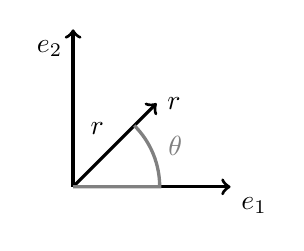
\begin{tikzpicture}[very thick]
        % \draw[fill=gray!30] (0,0)circle(1);
        \draw[->](0,0) --++ (2,0)node[below right ]{$\bm{e}_1$};
        \draw[->](0,0) --++ (0,2)node[below left ]{$\bm{e}_2$};
        \draw[->](0,0) --++ (45:1.5)node[right]{$r$}node[midway, above left]{$r$};
        \draw[gray](0,0) --++ (0:1.1)arc(0:45:1.1)node[below right]{$\;\;\;\theta$};
    \end{tikzpicture}   
	\begin{tikzpicture}[tdplot_main_coords,scale = 0.3]
		\draw[->,thick] (0,0,0) -- (6.5,0,0) node [pos=1.1] {$\bm{e}_1$};
		\draw[->,thick] (0,0,0) -- (0,6,0) node [pos=1.05] {$\bm{e}_2$};
		\draw[->,thick] (0,0,0) -- (0,0,5.5)  node [pos=1.05] {$\bm{e}_3$};   
		\tdplotsetcoord{P'}{7}{\thetavec}{\phivec}
    	\tdplotsetcoord{P''}{1}{90}{90+\phivec}
    	\tdplotsetcoord{P'''}{1}{90+\thetavec}{\phivec}
		\tdplotsetcoord{P}{6}{\thetavec}{\phivec}
		\draw[->] (0,0,0) -- (P) node [midway, above] {$r$};
		\draw[thick] (0,0,0) -- (2,4,0);
		\draw[dashed] (2,4,4) -- (2,4,0);
		\draw[dashed] (2,0,0) -- (2,4,0) node [pos=-0.1] {$x$};
		\draw[dashed] (0,4,0) -- (2,4,0) node [pos=-0.3] {$y$};
		\draw[dashed] (0,0,4) -- (2,4,4) node [pos=-0.1] {$z$};
		\draw[dashed, tdplot_main_coords] (4.47,0,0) arc (0:90:4.47);
		\node[fill=black, circle, inner sep=0.8pt] at (2,4,4) {};
		\tdplotdrawarc{(0,0,0)}{0.7}{0}{\phivec}{below}{$\phi$}
	    \tdplotsetthetaplanecoords{\phivec}
	    \tdplotdrawarc[tdplot_rotated_coords]{(0,0,0)}{0.5}{0}{\thetavec}{}{}
	    \node at (0,0.25,0.67) {$\theta$};
	\end{tikzpicture}

    \caption{Parametrization of the problem for 2D and 3D case.}
    \label{fig:schemeshpere}
\end{figure}
Now let's derive the first 4 moments for a 2D spherical particle. 
The zeroth moment reads as,
\begin{equation}
    \mathcal{G}^0 
    = \int_V  d\bm{y} 
    = \int_0^{2\pi}\int_0^{R}  d\bm{y} 
    = [\theta]_0^{2\pi}[r]_0^{R} 
    = 2\pi R
\end{equation}
where we used the notation depicted on the scheme \ref{fig:schemeshpere}.
The first moment as already mentioned is, $\mathcal{G}^1 = \int \bm{r}_\alpha dV = 0$.
Next, the second moment yields,
\begin{equation}
    (\mathcal{G}^2)_{ij}
    = \int_V r_ir_j d\bm{y} 
    = \int_0^{2\pi}\int_0^{R} r_ir_j d r dr d\theta 
    = \int_0^{R} r^3 dr \int_0^{2\pi} r_ir_j d\theta  
    = \frac{R^4}{4} \int_0^{2\pi} r_ir_j d\theta 
\end{equation}
where $\bm{r} = (\cos{\theta}, \sin{\theta})$. 
Then, 
\begin{equation}
    \mathcal{G}^2 = \frac{R^4}{4}\left[\begin{tabular}{cc}
        $\pi$&$0$\\
        $0$&$\pi$\\
    \end{tabular}
    \right].
\end{equation}
More generally the $l^{th}$ moment reads as, 
\begin{equation}
    (\mathcal{G}^l)_{i_1i_2\ldots i_l}
    = \frac{R^{l+2}}{l+2} \int_0^{2\pi} r_{i_1}r_{i_2}\ldots r_{i_l} d\theta 
\end{equation}
Then, two things can be shown. 
The first one, is that the components off-diagonal of $\mathcal{G}^l$ are null. 
The second, is that the values on the diagonal are the same. 
If we consider the sum on all indices, the product $r_{i_1}r_{i_2}\ldots r_{i_l}$ can be written $(\cos\theta+\sin\theta)^l$.
Moreover, 
\begin{equation}
    (\cos\theta+\sin\theta)^l  = \sum_{k=0}^l\binom{l}{k}\cos^k\theta\sin^{l-k}\theta
\end{equation}
Thus, the integral $\int_0^{2\pi} r_{i_1}r_{i_2}\ldots r_{i_l} d\theta$ always follows this form,
\begin{equation}
    \int_0^{2\pi} \cos^k\theta\sin^{l-k}\theta d\theta \;\;\;\forall k\leq l. 
    \label{eq:cossin}
\end{equation}
Now, we can note that the diagonal components $I$ and $II$ (i.e. the diagonal in the sense that all the indices are the same) are equal to,
\begin{equation}
    (\mathcal{G}^l)_{I}
    = \int_0^{2\pi} \cos^l d\theta\;\;\;
    (\mathcal{G}^l)_{II}
    = \int_0^{2\pi} \sin^l d\theta  
\end{equation}
Let's develop the first term, 
\begin{align*}
    (\mathcal{G}^l)_{I}
    &= \int_0^{2\pi} \cos^l d\theta\\
    &= \frac{1}{l} \left[\cos^{l-1}\theta\sin\theta \right]_0^{2\pi} + \frac{l-1}{l} \int_0^{2\pi} \cos^{l-2} d\theta.\\
\end{align*}
The first term on the right hands side is always null. 
Indeed, $\cos$ is pair at any power of, $l-1$, and $\sin$ is odd, thus the product of the two terms is an odd function. 
Moreover, the product between $\sin$ or $\cos$ are at least $2\pi$ periodic. 
Therefore, the integral taken between $0$ and $\pi$ is null, and the relation reduce to, 
\begin{equation*}
    (\mathcal{G}^l)_{I}
    = \int_0^{2\pi} \cos^l d\theta
    =  \frac{l-1}{l} \int_0^{2\pi} \cos^{l-2} d\theta\\
    =  \frac{l-1}{l}\frac{l-3}{l-2} \int_0^{2\pi} \cos^{l-4} d\theta\\
\end{equation*}
If we keep repeating the process we eventually arrive to the smallest power. 
Which is either $0$ or $1$ if we start by, respectively a number $l$ pair and a number $l$ odd.
Therefore, we pose $l = 2q$ in the first case and $l = 2q+1$ in the second, 
\begin{equation*}
    (\mathcal{G}^{2q})_{I}
    =  \frac{2q-1}{2q}\frac{2q-3}{2q-2} \int_0^{2\pi} \cos^{2q-4}\theta d\theta\\
    =  \prod^{q-1}_{k= 0}\frac{2q-2k-1}{2q-2k} \int_0^{2\pi}  d\theta\\
    =  \prod^{q-1}_{k= 0}\frac{2q-2k-1}{2q-2k} 2\pi\\,
\end{equation*}
and,
\begin{equation*}
    (\mathcal{G}^{2q+1})_{I}
    =  \prod^{q}_{k= 0}\frac{2q-2k}{2q-2k+1} \int_0^{2\pi} \cos \theta d\theta\\
    = 0.
\end{equation*}
Similar calculation can be done for the powers of $\sin$, and it yields the same results. 
Therefore, the diagonal components of the $l^{th}$ order tensor of a disk are, 
\begin{equation}
    \mathcal{G}_{I}^l=\mathcal{G}_{II}^l = \left\{\begin{tabular}{cc}
        $\prod^{q-1}_{k= 0}\frac{2q-2k-1}{2q-2k} 2\pi $& if $l = 2q$     \\
        $0 $        & if $l = 2q+1$
    \end{tabular}\right.
    \label{eq:cosl}
\end{equation}
In fact, if we can carry out similar calculations for the integral, \ref{eq:cossin}, we find that, 
\begin{equation}
    \int_0^{2\pi} \sin^k \cos^{l-k} dV = \frac{1}{2}\frac{k-1}{l-k-1} \int_0^{2\pi} \sin^{l-2}\theta \cos^{l-k+2}\theta d\theta.
\end{equation}
Note that taking $l = 2q$ or $l=2q+1$ leads to either $\sin^0\theta^{l-k+2q} $ or $\sin \theta^{l-k+2q+1}$ in the integral. 
Therefore, the integral of  $\sin \theta^{l-k+2q+1}$ between $0$ and $2\pi$ will ultimately cancel out. 
Therefore, we obtain the following relation in the non-null cases,
\begin{equation}
    \int_0^{2\pi} \sin^k \cos^{l-k} d\theta = \left\{\begin{tabular}{cc}
        $\prod^{q-1}_{n=0}\frac{2q-2n-1}{l-2q+2n+1} \int_0^{2\pi} \cos^{l} d\theta$& if $k = 2q$     \\
        $0 $        & if $l = 2q+1$
    \end{tabular}\right.
\end{equation}
Using \ref{eq:cosl} yields,
\begin{equation}
    \int_0^{2\pi} \sin^k \cos^{l-k} d\theta = \left\{\begin{tabular}{cc}
        $\prod^{q-1}_{n=0}\frac{2q-2n-1}{2r-2q+2n+1} \prod^{r-1}_{n= 0}\frac{2r-2n-1}{2r-2n} 2\pi $& if $k = 2q$ and $l = 2r$    \\
        $0$        & if $k = 2q  $ and $l = 2r +1$\\
        $0$        & if $k = 2q+1$ and $l = 2r$\\
        $0$        & if $k = 2q+1$ and $l = 2r +1$
    \end{tabular}\right.
\end{equation}
The remaining question is now, how to link the indexes of the tensor to the value of $k$.
If we consider a tensor of order $2$ it is easy to say that, 
\begin{equation}
    \mathcal{G}_{ij} = \delta_{ij} \frac{R^4}{4}\pi. 
\end{equation} 
For a $4^{th}$ order tensor it is given by, 
\begin{equation}
    \mathcal{G}_{ijkl} = (\delta_{ij}\delta_{kl} + \delta_{ik}\delta_{lj}) \frac{R^6}{8} \pi
\end{equation} 
we can deduce the pattern for the higher order tensor. 
Indeed, the non-null terms can be defined by the sum of all the possible product of $\delta$.
It can be shown that for a tensor of order $l$ the number of combination of $\delta$ is $n= 1+(l/2-1)l/2$.
}
\section{3D sphere shape tensor}
For spherical particles, it is possible to carry out similar calculation using spherical coordinate. 
Nevertheless, it is more convenient to use tensor calculation for this matter. 
Using spherical coordinates it follows,
\begin{align*}
    \mathcal{G}_{i_1i_2\ldots i_l}^l 
    &= \rho_d \int_{V_\alpha} \prod^l_{m=1}r^\alpha_{i_m} dV\\
    &= \rho_d \int_0^R r^{l+2} dr  
      \int_{S_\alpha} \prod^l_{m=1}r^\alpha_{i_m} dS\\
    &=\rho_d \frac{R^{l+3}}{l+3}
      \int_{S_\alpha}  n_{i_l} \prod^{l-1}_{m=1} r^\alpha_{i_m} dS\\
    &=\rho_d \frac{R^{l+3}}{l+3}
      \int_{V_\alpha}  \partial_{i_l} \left(\prod^{l-1}_{m=1} r^\alpha_{i_m}\right) dV\\
    &=\rho_d \frac{R^{l+3}}{l+3}\sum_{k=1}^{l-1} \delta_{i_l i_k}
      \int_{V_\alpha}  \prod^{l-1}_{\substack{m=1\\ m\neq k}} r^\alpha_{i_m} dV\\
\end{align*}
where we recognize the $l-2$ order shape tensor in the last expression. 
By carrying the same calculation for this tensor we can compute the original $l^{th}$ order shape tensor in a recursive manner. 
We note that all odds order shape tensor will reduce to a sum of $\int r^\alpha dV$ which is null. 
To conclude, the  $l^{th}$ shape tensor of any spherical particles is null for any odd order. 
Moreover, for even order tensor we can note that the components non-null are carried by Kronecker symbols which is the expression of isotropy of the particle. 
Indeed, repeating the previous formula leads to this expression,
\begin{align*}
    \mathcal{G}_{i_1i_2\ldots i_l}^l 
    &=\rho_d \frac{R^{l+3}}{l+3}\sum_{a=1}^{l-1} \delta_{i_l i_a}
      \int_{V_\alpha}  \prod^{l-1}_{\substack{m=1\\ m\neq a}} r^\alpha_{i_m} dV\\
    &=\rho_d \frac{R^{l+3}}{l+3}
    \frac{R^{l+1}}{l+1}\sum_{a=1}^{l-1} \delta_{i_l i_a}
    \sum_{\substack{b=1\\ b\neq a}}^{l-2} \delta_{i_{l-1} i_b}
      \int_{V_\alpha}  \prod^{l-2}_{\substack{m=1\\ m\neq a\\ m\neq b}} r^\alpha_{i_m} dV\\
    &=\rho_d \frac{R^{l+3}}{l+3}
    \frac{R^{l+1}}{l+1} 
    \ldots
    \frac{R^3}{3}
    V_\alpha
    \delta_{i_l i_a}
    \delta_{i_{l-1} i_b}
    \delta_{i_{l-2} i_c}
    \ldots
    \delta_{i_2i_1},
\end{align*}
In further developments we will refer to the product of all the scalar values with the letter $A^l$. 
Therefore, 
\begin{equation}
    \mathcal{G}_{i_1i_2\ldots i_l}^l 
    = A^l V_\alpha
    \delta_{i_l i_a}
    \delta_{i_{l-1} i_b}
    \delta_{i_{l-2} i_c}
    \ldots
    \delta_{i_2i_1},
    \label{eq:shapeT}
\end{equation}
where it is implies that we sum the expression on $a$, $b$, $c\ldots$ in their respective range. 

From this formula we can derive the theoretical expression of the second order shape tensor. 
\begin{equation*}
    \mathcal{G}_{ij} 
    = \rho \int_{V_\alpha} \textbf{r} \textbf{r} dV 
    = \rho \int_0^R r^2 dr \int_{S_\alpha} \textbf{n} \textbf{n}  dS 
    = \rho \frac{R^3}{3} \int_{V_\alpha} \grad \textbf{n} dV
    = \rho \frac{R^2}{3} V_\alpha \delta_{ij}
\end{equation*}
where we have used the relation $\frac{\partial}{\partial y_i}n_j = R^{-1} \delta_{ij}$, note that this is equivalent to the regular calculation, i.e. 
\begin{equation*}
    \mathcal{G}_{zz} 
    = \int_{V_\alpha} r^2 \cos^2{\theta} dV 
    = \int_{0}^R \int_{\phi = 0}^{2\pi} \int_{\theta = 0}^{\pi} r^4 \cos^2{\theta} \sin{\theta} drd\theta d\phi
    = \frac{4R^5}{15}\pi
\end{equation*}

POZRIKIDIS P 217 

\tb{
\subsection{Second order shape tensor for elongated particles}

Now let's consider any particles oriented along its axis of revolution $\bm{p}$. 
Any shape tensor can be expressed as $\mathcal{G}^2_{ij} = p_ip_j G_{||} + (\delta_{ij} - p_ip_j) G_{\bot}$ where $G_\bot$ and $G_{||}$ are constants value corresponding to Eigenvalues values of the shape tensor. 
For antisymmetric particles the Eigenvectors are aligned with the axis of revolution. 
Therefore, using a polar coordinates frame $(r, \theta, z)$ aligned with $\bm{p}$ yields the following formulas for the Eigenvalues of the shape tensor :
\begin{equation}
    G_{||} = \int_V z z dV \;\;\;\;\;\;
    G_{\bot} = \int_V r^2 \cos^2\theta dV.
\end{equation}
As an example let's now consider cylindrical particles of radius $R$ and aspect ratio $\chi$.
Then,
\begin{equation}
    G_{||} = \int_0^R\int_{-\chi R}^{\chi R} \int_0^{2\pi} z z r dr d\theta dz
    = \frac{2}{3}\pi R^5 \chi^3
\end{equation}
\begin{equation}
    G_{\bot} = \int_0^R\int_{-\chi R}^{\chi R} \int_0^{2\pi} r^3 \cos^2\theta dr d\theta dz
    = \frac{1}{2} \pi R^5 \chi.
\end{equation}
If we consider a 2D ellipse where the main axis are of length $a$ and $b$ we can express the shape tensor as,
\begin{equation}
    \mathcal{G}_{11}
    = \frac{\pi}{4}a^3b,
    \;\;\;\; 
    \mathcal{G}_{22}
    = \frac{\pi}{4}b^3a. 
    \label{eq:shapeellipse}
\end{equation}

}
\section{Kinematic equations for the $l^{th}$ order surface tensor.}

Here is the proof of the surface tensor derivations,
\begin{equation*}
    \ddt \int_{S_\alpha} dS 
    = \int_{S_\alpha} \grad_I \cdot \textbf{u}_I dS
\end{equation*}
\begin{equation*}
    \ddt \int_{S_\alpha} \textbf{r} dS 
    = \int_{S_\alpha} \textbf{r} \grad_I \cdot \textbf{u}_I dS
    + \int_{S_\alpha} \textbf{u}_I  \cdot (\textbf{I}-\textbf{nn}) dS
    - \textbf{u}_\alpha \int_{S_\alpha} dS
\end{equation*}
\begin{equation*}
    \ddt \int_{S_\alpha} \textbf{rr} dS 
    = \int_{S_\alpha} \textbf{rr} \grad_I \cdot \textbf{u}_I dS
    + 2 \int_{S_\alpha}\textbf{r} \textbf{u}_I  \cdot (\textbf{I}-\textbf{nn}) dS
    - \int_{S_\alpha} \textbf{u}_\alpha \textbf{r} + \textbf{r}  \textbf{u}_\alpha dS
\end{equation*}
Now we can write the derivation for an arbitrary tensor orders, using the Reynolds transport theorem it reads, 
\begin{align*}
    \ddt \int_{S_\alpha} \pri{1}{n}dS
    &= \int_{S_\alpha} \pddt \left(
        \pri{1}{n}
    \right) dS
    + \int_{S_\alpha} 
    \partial_k^I  \left(
        u^I_k \pri{1}{n}
    \right)dS \\
    &= - \sum_{e=1}^n u^\alpha_{i_e} \int_{S_\alpha} 
        \prod_{\substack{m = 1 \\m \neq e}}^{n} r_{i_m}
     dS
    + \int_{S_\alpha} u^I_k
    \partial_k^I  \left(
         \prod_{m=1}^{n} r_{i_m}
    \right)dS \\
    &+ \int_{S_\alpha} 
    \prod_{m=1}^{n} r_{i_m}
    \partial_k^I u^I_k 
    dS \\
\end{align*}
Using the definition of the surface derivative
\begin{align*}
    \ddt \int_{S_\alpha} \pri{1}{n}dS
    &= \int_{S_\alpha} 
    \prod_{\substack{m = 1 \\m \neq e}}^{n} r_{i_m}
    \partial_k^I u^I_k 
    dS 
    - \sum_{e=1}^n u^\alpha_{i_e} \int_{S_\alpha} 
    \prod_{\substack{m = 1 \\m \neq e}}^{n} r_{i_m}dS \\
    &+ \sum_{e=1}^n \int_{S_\alpha} u^I_k
    \prod_{\substack{m = 1 \\m \neq e}}^{n} r_{i_m}
    (\delta_{ki_e} - n_kn_{i_e}) dS \\
    &= \int_{S_\alpha} 
    \prod_{\substack{m = 1 \\m \neq e}}^{n} r_{i_m}
    \partial_k^I u^I_k dS 
    + \sum_{e=1}^n  \int_{S_\alpha} (w^I_{i_e} - u^I_kn_kn_{i_e}) 
    \prod_{\substack{m = 1 \\m \neq e}}^{n} r_{i_m}dS \\
\end{align*}
Thus, 
\begin{align*}
    \int_{S_\alpha} 
    \prod_{\substack{m = 1 \\m \neq e}}^{n} r_{i_m}
    \partial_k^I u^I_k dS 
    &=
    \ddt \int_{S_\alpha} \pri{1}{n}dS
    + \sum_{e=1}^n u^\alpha_{i_e} \int_{S_\alpha} 
    \prod_{\substack{m = 1 \\m \neq e}}^{n} r_{i_m}dS \\
    &+ \sum_{e=1}^n \int_{S_\alpha} u^I_k
    \prod_{\substack{m = 1 \\m \neq e}}^{n} r_{i_m}
    (n_kn_{i_e} - \delta_{ki_e}) dS \\
\end{align*}


\section{Equations for arbitrary moment of mass.}
Let consider the $l^{th}$ order shape tensor $\mathcal{G}^l_\alpha$ of a given particle $\alpha$. 
In this section we demonstrate how to take the time derivative of any tensor $\mathcal{G}^l_\alpha$. 
In this section we are going to make use of Einstein summation convention to represent the arbitrary order tensors. 
Besides, for a better understanding of the equations we use the notation $\bm{r}^\alpha$ for $\bm{r}_\alpha$ (which is the distance between the center of mass and a given point). 
The shape tensor of any order $l$ is defined by,
\begin{equation}
    \mathcal{G}_{i_1i_2\ldots i_l}^l = \rho_d \int_{V_\alpha} \prod^l_{m=1}r^\alpha_{i_m} dV,
\end{equation}
where each $i_m$ represent different indices. 
Then taking the time derivative and using \ref{eq:timetransport} gives the following relation,
\begin{multline}
    \frac{d}{dt}\mathcal{G}_{i_1i_2\ldots i_l}^l 
    = \rho_d \int_{V_\alpha} \left[ \frac{\partial}{\partial t} \left(\prod^l_{m=1}r^\alpha_{i_m}\right) 
    + \frac{\partial}{\partial y_k} \left(u_k\prod^l_{m=1}r^\alpha_{i_m}\right) \right]dV\\
    +\int_{S_\alpha} \prod^l_{m=1}r^\alpha_{i_m} \rho_d \left((u_I)_k - u_k\right) n_k^\alpha dS,
\end{multline}
where we recall that the second term is due to mass transfer and will be noted $T^l_\alpha$ for compactness. 
Using, the product rule on the derivative yields the following relation :
\begin{multline}
    \frac{d}{dt}\mathcal{G}_{i_1i_2\ldots i_l}^l 
    = \rho_d \int_{V_\alpha} \sum_{e=1}^l \left[ \prod^l_{\substack{ m=1 \\   m \neq e}}r^\alpha_{i_m} \frac{\partial}{\partial t} \left(r_{i_e}\right) 
    + \prod^l_{m=1}r^\alpha_{i_m} \frac{\partial}{\partial y_k} \left(u_k\right) 
    \right.\\
    \left.
    + u_k \frac{\partial}{\partial y_k} \left(\prod^l_{m=1}r^\alpha_{i_m}\right) \right]dV
    +T^\alpha_{i_1i_2\ldots i_l},
\end{multline}
where we can recognize the second term as the divergence of the velocity, which is null since the fluid is incompressible. 
Now, by making use of the product rule on the third term it yields,
\begin{equation}
    \frac{d}{dt}\mathcal{G}_{i_1i_2\ldots i_l}^l 
    = \rho_d \int_{V_\alpha} \sum_{e=1}^l \prod^l_{\substack{ m=1 \\   m \neq e}} r^\alpha_{i_m}\left[ \frac{\partial}{\partial t} \left(r_{i_e}\right) 
    + u_k \frac{\partial}{\partial y_k} \left(r_{i_e}\right) \right]dV
    +T^\alpha_{i_1i_2\ldots i_l},
\end{equation}
The term within the brackets can be simplified thanks to \ref{eq:momentofmomentumDev} as the fluctuation of the velocity around the center of mass noted $\bm{w}^\alpha$.
\begin{equation}
    \frac{d}{dt}\mathcal{G}_{i_1i_2\ldots i_l}^l 
    = \rho_d \sum_{e=1}^l \int_{V_\alpha}  \prod^l_{\substack{ m=1 \\   m \neq e}} r^\alpha_{i_m} w_{i_e}dV
    +T^\alpha_{i_1i_2\ldots i_l}.
\end{equation}
In the summation sign we can recognize the $(l-1)^{th}$ moment of momentum tensor. 
\begin{equation}
    \frac{d}{dt}\mathcal{G}_{i_1i_2\ldots i_l}^l 
    = \sum_{e=1}^l P^\alpha_{i_1\ldots i_e\ldots i_l}
    +T^\alpha_{i_1i_2\ldots i_l}.
\end{equation}
Each terms in the sum is just the same tensor where we have permuted the indices. 
All the possible permutations are in the sum since there is only two different vectors, i.e. $\bm{r}^\alpha$ and $\bm{w}^\alpha$, and $\bm{w}^\alpha$ takes all the places among the $\bm{r}^\alpha$.
Furthermore, the sum of all the permutations of a tensor is proportional to its symmetric part \citep{itin2022decomposition}. 
Thus, we define the $^\text{Sym}$ operator which return the symmetric part of any $l^{th}$ order tensor. 
In tensor form the previous relation is then,
\begin{equation}
    \frac{d}{dt}\mathcal{G}^l 
    = l (\bm{P}_\alpha^l)^{\text{Sym}}
    +\bm{T}^\alpha.
    \label{eq:dt_G_alpha_l}
\end{equation}
The rate of change of the shape of the particle is therefore linked directly to its own moment of momentum. 
But it does not depend on the antisymmetric part. 
Which mean that the angular momentum do not play any role in the change of the shape. 
Next, we apply the particular average to this set of equations using \ref{eq:partia}.
It yields a $l$ order equation, 
\begin{equation}
    \partial_t\left(n\left<\mathcal{G}_{i_1i_2\ldots i_l}^l\right>^p\right) 
    +\partial_k\left(n\left<u_k\mathcal{G}_{i_1i_2\ldots i_l}^l\right>^p\right) 
    = n\;l\left<(P^\alpha_{i_1\ldots i_e\ldots i_l})^\text{Sym}\right>
    +n\left<T^\alpha_{i_1i_2\ldots i_l}\right>.
\end{equation}
Then, we obtained a set of $l$ equations which describe the evolution and the transport of the averaged shape properties. 
In the following we review the meaning for each of the first orders equations. 
Besides, we neglect the mass transfer term as it is not useful for our application. 
\tb{In those equations we must add the conservation of volume condition.
Look into \citet{maffettone1998equation}}

\tb{
\subsection{Equation at the first order}
At the first order we have the following relation, 
\begin{equation}
    \frac{d}{dt}\mathcal{G}^1 
    =  \frac{\partial}{\partial t} \rho_d \int_{V_\alpha} \bm{r}_\alpha dV 
    = \rho_d \int_{V_\alpha} \bm{w}_\alpha dV
    = 0. 
\end{equation}
We recall that $\bm{r}_\alpha$ is defined such that $\int_{V_\alpha} \bm{r}_\alpha dV$ is null. 
Therefore, this relation leads to a null term. 

\subsection{Second order relation}
At the second order the relation is, 
\begin{equation}
    \frac{d}{dt}\mathcal{G}^2
    = 2 (\bm{P}_\alpha^2)^{\text{Sym}}. 
    \label{eq:dGdt}
\end{equation}
Therefore the following calculation might not make sense
Thus, the rate of change of the shape of the particle is equal to the symmetric part of the moment of momentum. 
Let's study this equation in the linear displacement hypothesis to get a more physical conclusion of the matter. 
From the previous section (\ref{eq:linear2}), and by keeping only the symmetric part of $\bm{P_\alpha}$ one can deduce, 
\begin{equation}
    \frac{d}{dt}\mathcal{G}^2
    = 2 \bm{E}_\alpha \cdot \mathcal{G}^2. 
\end{equation}
Which gives us a set of $d^2$ (where $d$ is the dimension) linear differential equations for the shape tensor, namely
\begin{equation}
    \frac{d}{dt}\mathcal{G}^2_{ij}
    = 2 E^\alpha_{ik}  \mathcal{G}^2_{kj}. 
\end{equation}


}
\section{Dynamical equations for the $l^{th}$ order momentum tensor.}
Let consider the $l^{th}$ order momentum tensor $\bm{P}^l_\alpha$ of a given particle $\alpha$. 
In this section we demonstrate how to take the time derivative of any tensor $\bm{P}^l_\alpha$. 
We are going to make use of Einstein summation convention to represent the arbitrary order tensors. 
The momentum tensor of any order $l$ is defined by,
\begin{equation}
    P_{i_1i_2\ldots i_l}^{l} = \rho_d \int_{V_\alpha} \prod^{l-1}_{m=1}r^\alpha_{i_m} u_{i_l} dV,
\end{equation}
Then taking the time derivative and using \ref{eq:timetransport} gives the following relation,
\begin{multline*}
    \frac{d}{dt}P_{i_1i_2\ldots i_l}^l 
    = \rho_d \int_{V_\alpha} \left[ \frac{\partial}{\partial t} \left(\prod^{l-1}_{m=1}r^\alpha_{i_m} u_{i_l}\right) 
    + \frac{\partial}{\partial y_k} \left(u_k\prod^{l-1}_{m=1}r^\alpha_{i_m} u_{i_l}\right) \right]dV\\
    +\int_{S_\alpha} \prod^{l-1}_{m=1}r^\alpha_{i_m} u_{i_l} \left((u_I)_k - u_k\right) n_k^\alpha dS.
\end{multline*}
The last term is the moment of momentum of mass transfer and will be referred as $(T_u^\alpha)_{i_1i_2\ldots i_l}$ 
using the product rule for the derivation of the terms inside the first integral gives, 
\begin{multline*}
    \frac{d}{dt}P_{i_1i_2\ldots i_l}^l 
    = 
    \rho_d \int_{V_\alpha} u_{i_l}\left[  \frac{\partial}{\partial t} \left(\prod^{l-1}_{m=1}r^\alpha_{i_m} \right) 
    + u_k \frac{\partial}{\partial y_k} \left(\prod^{l-1}_{m=1}r^\alpha_{i_m}\right) \right]dV\\
    +\rho_d \int_{V_\alpha}  \prod^{l-1}_{m=1}r^\alpha_{i_m} \left[ 
    \frac{\partial}{\partial t} \left(u_{i_l}\right) 
    + \frac{\partial}{\partial y_k} \left(u_k u_{i_l}\right) 
    \right]dV
    +(T_u^\alpha)_{i_1i_2\ldots i_l},
\end{multline*}
Using the same calculation as in the previous section for the first term, and using,  the development carried in \ref{chap:avg} for the second leads to, 
\begin{multline*}
    \frac{d}{dt}P_{i_1i_2\ldots i_l}^l 
    = 
    \rho_d \sum_{e=1}^{l-1} \int_{V_\alpha} u_{i_l}  \prod^{l-1}_{\substack{ m=1 \\   m \neq e}} r^\alpha_{i_m} w_{i_e}dV\\
    +\rho_d \int_{V_\alpha}  \prod^{l-1}_{m=1}r^\alpha_{i_m} \left[ 
    \partial_k \sigma_{ki_l} + b_{i_l} + f^\sigma_{i_l}   
    \right]dV
    +(T_u^\alpha)_{i_1i_2\ldots i_l}.
    \label{eq:B68}
\end{multline*}
Besides, we can derive the following relation,
\begin{multline*}
    \partial_k\left(\prod^{l-1}_{m=1}r^\alpha_{i_m}  \sigma_{ki_l}\right)
    = \prod^{l-1}_{m=1}r^\alpha_{i_m} \partial_k \sigma_{ki_l} 
    + \sigma_{ki_l} \partial_k \prod^{l-1}_{m=1}r^\alpha_{i_m}\\
    = \prod^{l-1}_{m=1}r^\alpha_{i_m} \partial_k \sigma_{ki_l} 
    + \sum^{l-1}_{e =1} \sigma_{i_ei_l} \prod^{l-1}_{\substack{m=1\\ m\neq e}}r^\alpha_{i_m}  
\end{multline*}
Therefore, term involving the divergence of the stress in \ref{eq:B68} can be rewritten as so, 
\begin{equation}
    \int_{V_\alpha} \prod^{l-1}_{m=1}r^\alpha_{i_m} \partial_k \sigma_{ki_l} dV
    =
    \int_{V_\alpha} \partial_k\left(\prod^{l-1}_{m=1}r^\alpha_{i_m}  \sigma_{ki_l}\right) dV 
    -\int_{V_\alpha} \sum^{l-1}_{e=1} \sigma_{i_ei_l}  \prod^{l-1}_{\substack{m=1\\ m\neq e}}r^\alpha_{i_m}  dV
\end{equation}
Using the divergence theorem on the first term yields,  
\begin{equation}
    \int_{V_\alpha} \prod^{l-1}_{m=1}r^\alpha_{i_m} \partial_k \sigma_{ki_l} dV
    =
    \int_{S_\alpha} \prod^{l-1}_{m=1}r^\alpha_{i_m}  \sigma_{ki_l}^fn_k dS 
    -\int_{V_\alpha} \sum^{l-1}_{e=1} \prod^{l-1}_{\substack{m=1\\ m\neq e}}r^\alpha_{i_m}  \sigma_{i_ei_l}^d dV,
\end{equation}
noticing that the first term represent the $l^h$ order of the hydrodynamic moment and the terms in brackets in \ref{eq:B68} represent the $l^{th}$ moment of the body forces and surface tension force,
\begin{multline}
    \frac{d}{dt}P_{i_1i_2\ldots i_l}^\alpha
    = 
    (M^h_\alpha)_{i_1\ldots i_l}
    +(M^\sigma_\alpha)_{i_1\ldots i_l}
    +(M^b_\alpha)_{i_1\ldots i_l}\\
    +\rho_d  \int_{V_\alpha} \sum_{e=1}^{l-1}  \prod^{l-1}_{\substack{ m=1 \\   m \neq e}} r^\alpha_{i_m} w_{i_e} u_{i_l}dV
    -\rho_d\int_{V_\alpha} \sum^{l-1}_{e=1} \prod^{l-1}_{\substack{m=1\\ m\neq e}}r^\alpha_{i_m}  \sigma_{i_ei_l}^d dV
    +(T_u^\alpha)_{i_1i_2\ldots i_l}.
    \label{eq:dt_P_order_l}
\end{multline}
Furthermore, as a consequence of the summation, the $5^{th}$ term on the right hands side is symmetric on all indices from $1$ to $l-1$.
Besides, the stress tensor is by definition symmetric on its own indices, i.e. $i_e$ and $i_l$. Therefore, this term is symmetric on all its indices and will vanish if one takes the antisymmetric part of the equation. 
By applying the decomposition of the velocity $u_i = u^\alpha_i + w_i$ we obtain a fully symmetric tensor plus the moments of the fluctuations times the mean velocity.
Knowing that it is possible to derive two distinct equations, one for the antisymmetric part and symmetric part. 
Using \ref{eq:Gorderl} the equation for the symmetric part reads as,
\begin{multline*}
    \frac{d^2}{dt^2}G_{i_1i_2\ldots i_l}^\alpha
    = 
    (S^h_\alpha)_{i_1\ldots i_l}
    +(S^\sigma_\alpha)_{i_1\ldots i_l}
    +(S^b_\alpha)_{i_1\ldots i_l}\\
    +\rho_d  \int_{V_\alpha} \sum_{e=1}^{l-1}  \prod^{l-1}_{\substack{ m=1 \\   m \neq e}} r^\alpha_{i_m} w_{i_e} u_{i_l}dV
    -\rho_d\int_{V_\alpha} \sum^{l-1}_{e=1} \prod^{l-1}_{\substack{m=1\\ m\neq e}}r^\alpha_{i_m}  \sigma_{i_ei_l}^d dV
    +(T_u^\alpha)_{i_1i_2\ldots i_l}.
\end{multline*}
Which is the equation of state of the particle shape tensor. 
And the antisymmetric part yields, 
\begin{multline*}
    \frac{d^2}{dt^2}G_{i_1i_2\ldots i_l}^\alpha
    = 
    (S^h_\alpha)_{i_1\ldots i_l}
    +(S^\sigma_\alpha)_{i_1\ldots i_l}
    +(S^b_\alpha)_{i_1\ldots i_l}\\
    +\rho_d  \int_{V_\alpha} \sum_{e=1}^{l-1}  \prod^{l-1}_{\substack{ m=1 \\   m \neq e}} r^\alpha_{i_m} w_{i_e} u_{i_l}dV
    -\rho_d\int_{V_\alpha} \sum^{l-1}_{e=1} \prod^{l-1}_{\substack{m=1\\ m\neq e}}r^\alpha_{i_m}  \sigma_{i_ei_l}^d dV
    +(T_u^\alpha)_{i_1i_2\ldots i_l}.
\end{multline*}

Anyhow, it is now possible ti apply the particular average the transport of momentum equation yielding, 
\begin{multline*}
    \partial_t\left(n\left<\mathcal{P}_{i_1i_2\ldots i_l}^\alpha\right>^p\right)
    +\partial_k\left(n\left<u_k\mathcal{P}_{i_1i_2\ldots i_l}^\alpha\right>^p\right)
    =
    \pavg{M^\alpha_{i_1\ldots i_l}}\\
    +\rho_d \pavg{ \int_{V_\alpha} \sum_{e=1}^{l-1}  \prod^{l-1}_{\substack{ m=1 \\   m \neq e}} r^\alpha_{i_m} w_{i_e} u_{i_l}dV}
    -\rho_d \pavg{\int_{V_\alpha} \sum^{l-1}_{e=1} \prod^{l-1}_{\substack{m=1\\ m\neq e}}r^\alpha_{i_m}  \sigma_{i_ei_l}^d dV}\\
    + \pavg{T^\alpha_{i_1i_2\ldots i_l}},
\end{multline*}
for the moment of momentum, were
$M^\alpha_{i_1\ldots i_l}$ is the sum of the moments due to the hydrodynamic forces, the surface tension forces and the body forces.

\subsection*{Arbitrary order moments equation}

Let's define the arbitrary moment of the tensor $f$, by, 
\begin{equation*}
    Q_{i_1\ldots i_n}
    = \int_{V_\alpha} 
    \pri{1}{n} f dV
\end{equation*}
Then,
\begin{multline*}
    \ddt Q_{i_1\ldots i_n}
    =\int_{V_\alpha} \left[ \partial_t \left(\pri{1}{n}f\right) 
    + \partial_k \left(u_k \pri{1}{n}f\right) \right]dV\\
    +\int_{S_\alpha} \pri{1}{n} f \left(u^I_k - u_k\right) n_k dS.
\end{multline*}
Using the product rule on the derivatives yields, 
\begin{multline*}
    \ddt Q_{i_1\ldots i_n}
    =\int_{V_\alpha} f \left[ \partial_t \left(\pri{1}{n}\right) 
    + u_k \partial_k \left( \pri{1}{n}\right) \right]dV\\
    +\int_{V_\alpha} \pri{1}{n} \left[ \partial_t \left(f\right) 
    +  \partial_k \left(u_k f \right) \right]dV\\
    +\int_{S_\alpha} \pri{1}{n} f \left(u^I_k - u_k\right) n_k dS.
\end{multline*}
From similar arguments as before one can easily show that, 
\begin{multline*}
    \ddt Q_{i_1\ldots i_n}
    = \sum_{e=1}^{n} \int_{V_\alpha} f  \prod^{n}_{\substack{ m=1 \\   m \neq e}} r_{i_m} w_{i_e}dV
    +\int_{V_\alpha} \pri{1}{n} \grad\cdot\mathbf{\Phi} dV\\
    + \int_{V_\alpha} \pri{1}{n} \textbf{S} dV
    +\int_{S_\alpha} \pri{1}{n} f \left(u^I_k - u_k\right) n_k dS.
\end{multline*}
The second term can be reformulated such as,
\begin{align*}
    \int_{V_\alpha} \pri{1}{n} \grad\cdot\mathbf{\Phi} dV
    &= \int_{S_\alpha} \grad \cdot \left(\pri{1}{n} \mathbf{\Phi} \right)dV
    - \int_{V_\alpha} \mathbf{\Phi} \cdot \grad \left(\pri{1}{n} \right)dV\\
    &= \int_{S_\alpha} \pri{1}{n} \mathbf{\Phi} \cdot \textbf{n}dS
    -\sum_{e=1}^{n} \int_{V_\alpha} \mathbf{\Phi}  \prod^{n}_{\substack{ m=1 \\m \neq e}} r_{i_m}  dV
\end{align*}
Including this relation into the former equation yields, 
\begin{multline*}
    \ddt Q_{i_1\ldots i_n}
    = \sum_{e=1}^{n} \int_{V_\alpha} \prod^{n}_{\substack{ m=1 \\   m \neq e}} r_{i_m} (w_{i_e}f  - \Phi)dV
    +\int_{S_\alpha} \pri{1}{n} \mathbf{\Phi} \cdot \textbf{n}dS\\
    + \int_{V_\alpha} \pri{1}{n} \textbf{S} dV
    +\int_{S_\alpha} \pri{1}{n} f \left(u^I_k - u_k\right) n_k dS.
\end{multline*}
Then it is possible from this equation to carry out a particular average but also to get the local scale equations. 
Indeed, if we consider $V_\alpha$ as being a fixed control volume the above equality can be rewritten such as, 
\begin{multline*}
    \pddt \left(\pri{1}{n}f\right)
    + \grad \cdot \left(\pri{1}{n}f \textbf{u}\right)
    = n  \pri{1}{n-1}  (w_{i_n}f  - \Phi)\\
    + \pri{1}{n} \textbf{S} 
    + \grad \cdot \left( \pri{1}{n} \mathbf{\Phi} \right)
    \label{ap:eq:dt_rrf}
\end{multline*}


\subsection{On the first hydrodynamic moment and its contribution.}

While providing closure term for the first moment the user must know which part is function of the local pressure since it is absolute. 
We recall that the first hydrodynamic moment of a particle reads as,
\begin{equation}
    (M^h_\alpha)_{ij} 
    = \int_{S_\alpha} r^\alpha_i \sigma_{jk} n_k dS.
\end{equation}
In this section we discuss the different contribution from the viscous and pressure stress to the first moment tensor by investigating the specific case of a particle in a uniform flow. 
We consider a flow where pressure can be express as the sum of a constant pressure $p_0$, a constant gradient along the $z$ coordinate, and a fluctuation part $p'$, thus $p =p_0 + f_b z + p'$ where $p'$ is the fluctuation and $f_b$ the constant gradient ($f_b = \rho_f g$ is the case of buoyant flows). 
Therefore, the stress tensor reads as, $\sigma_{jk} = -p \delta_{jk} + \mu_f (\partial_j u_k+\partial_k u_j)$.
Besides, the particles are assumed spherical, thus $r_i = n_i R$ over the surface $S_\alpha$, where $R$ is the radius. 
Injecting the previous facts in the first moment expression gives,
\begin{equation}
    (M^h_\alpha)_{ij} 
    = - p_0 \int_{S_\alpha} r_i n_j dS
    - f_b \int_{S_\alpha} r_i n_j z dS
    - \int_{S_\alpha} r_i n_j p' dS
    + \int_{S_\alpha} r_i n_k \mu_f (\partial_j u_k+\partial_k u_j) dS
    \label{eq:Fistmomentdec}
\end{equation}
The viscous and pressure fluctuation part are function of local property of the flow, 
consequently they cannot be computed theoretically. 
So, let's focus on the first and second terms in the case of spherical particles. 
Using spherical coordinate, any point, $\bm{r} = (r\sin\theta \cos\phi,\; r\sin\theta \sin\phi,\; r\cos\theta )$,
Therefore the first term can be written, 
\begin{equation}
    p_0 \int_{S_\alpha} r_i n_j dS
    = p_0 R^3 \int_{0}^{2\pi}\int_{0}^\pi n_i n_j \sin\theta d\theta d\phi.
\end{equation}
Then, we have to compute the integral of each member of the following matrix,
\begin{multline}
    p_0 R^3 \int_{0}^{2\pi}\int_{0}^\pi n_i n_j \sin\theta d\theta d\phi
    =\\
     p_0 R^3 \int_{0}^{2\pi}\int_{0}^\pi
    \left[
        \begin{matrix}
            \sin^3\theta \cos^2\phi & \sin^3\theta  \cos\phi \sin\phi
            &\cos\theta\sin^2\theta \cos\phi\\
            \sim& \sin^3\theta \sin^2\phi & \sin^2\theta \cos\theta\sin\phi \\
            \sim& \sim & \sin\theta \cos^2\theta \\
        \end{matrix}
    \right]
    d\theta d\phi,
\end{multline}
by using the separation of variable method one can compute any of these integrals and find that only the diagonal components remain, and we find that, 
\begin{equation}
    p_0 R^3 \int_{0}^{2\pi}\int_{0}^\pi n_i n_j \sin\theta d\theta d\phi
    = \frac{4}{3}  p_0 R^3 \pi \delta_{ij}.
\end{equation}
Likewise, the second term of \ref{eq:Fistmomentdec} reads as,
\begin{multline}
    f_b \int_{S_\alpha} r_i n_j z dS
    =\\
     f_b R^3 \int_{0}^{2\pi}\int_{0}^\pi
    \left[
        \begin{matrix}
            \sin^3\theta \cos\theta \cos^2\phi & \sin^3\theta \cos\theta \cos\phi \sin\phi
            &\cos^2\theta\sin^2\theta \cos\phi\\
            \sim& \sin^3\theta \cos\theta \sin^2\phi & \sin^2\theta \cos^2\theta\sin\phi \\
            \sim& \sim & \sin\theta \cos^3\theta \\
        \end{matrix}
    \right]
    d\theta d\phi,
\end{multline}
Since the function depending on $\theta$ are antisymmetric around $\pi/2$ the integrals of the diagonal term are null.
In addition, the anti-diagonal components must be null due to the anisotropy of the geometry, and they are.  
In conclusion, the absolute pressure contribute to the first moment as $ \frac{4}{3}  p_0 R^4 \pi \delta_{ij}$, and the pressure gradient do not. 
Consequently, care must be taken while computing the stresslet on DNS software since we do not want the absolute pressure to appear in the results. 


\subsection{On the first moment of the surface tension}
The aim of this part is to express the link between the first order moment of the surface tension, i.e. $\bm{M}^\sigma_\alpha$ to the shape of the particle, i.e. the shape tensor $\mathcal{G}_\alpha$.
In the moment of momentum equation we see appear the unique contribution to the surface tension on the averaged equation though the first moment of the surface tension defined as,
\begin{equation}
    (M^\sigma_\alpha)_{ij}=\int_{S_\alpha}r^\alpha_i f^\sigma_j dS
\end{equation}
using the definition of the surface forces with a constant surface tension $\sigma$ gives, 
\begin{equation}
    (M^\sigma_\alpha)_{ij}=\int_{S_\alpha}r^\alpha_i \sigma \kappa n_j dS
\end{equation}
where $\kappa = -\nabla \cdot \bm{n}$ is the curvature of the surface. 
For spherical particles $\kappa = 1/R$ where $R$ is the radius of the sphere.
Therefore, the moment over the surface of the particle reads,
\begin{align}
    (M^\sigma_\alpha)_{ij}
    &= \frac{\sigma}{R}\int_{S_\alpha}r^\alpha_i n_j dS
    = \frac{\sigma}{R}\int_{V_\alpha} \partial_j r^\alpha_i dV
    = V_\alpha \frac{\sigma}{R}  \delta_{ij}\\
    &
    = \frac{4}{3} \pi R^2 \sigma  \delta_{ij} 
    \text{ for sphere, and  } 
    \pi R \sigma  \delta_{ij} 
    \text{ for circle.} 
    )
    \label{eq:MtensionCric}
\end{align}
The moment is fully isotropic, and in the static isolated case, it clearly expresses the hydrostatic pressure due to surface force applied on a spherical particle. 

For arbitrary shaped particles it gives we need to decompose the problem in two sub-problems. 
Any geometry can be decomposed by a static sphere of radius $R_m(t)$ plus a perturbed shape which can be described with a $2\pi$ periodic function $f(t,\theta,\phi)$. 
Similarly, we can define the curvature $\kappa$ as the sum of $\kappa_1$, which is the mean curvature and $\kappa_2$ is the fluctuations from the surface of the spherical geometry. Then,
\begin{equation}
    (M^\sigma_\alpha)_{ij}
    =\int_{S_\alpha}r^\alpha_i \sigma \kappa_1 n_j dS
    +\int_{S_\alpha}r^\alpha_i \sigma \kappa_2 n_j dS\\
    = \underbrace{\frac{4}{3} \pi \sigma R_m^2(t)  \delta_{ij}}_{\text{Spherical}}
    +
    \underbrace{\int_{S_\alpha(t)}r^\alpha_i \sigma \kappa_2 n_j dS}_{\text{Deviatoric}},
\end{equation}
where we can clearly identify the spherical and deviatoric part of the moment due to surface forces,
and we empathize the dependency of the surface $S_\alpha(t)$ with time. 
Before going further it is important to note that the deviatoric part of this tensor isn't necessarily symmetric, consequently it must appear in the torque equation.
Now we let's consider a 2D deformable ellipsoid of volume, $\pi R_m^2$, and as semi-minor axis $a(t)$ and $b(t)$. 
By exploiting the conservation of volume property we obtain the following relation, 
$a(t) = R^2_m/b(t)$. 
The coordinates an ellipse can be represented by $\bm{r} = (a(t) \cos\theta, b(t)\sin\theta)$. 
Besides, in 2D it can be shown (see \citet{tryggvason2011direct}) that the normal and curvature of the surface, respectively $\bm{n}$ and $\kappa$ can be express as,
\begin{equation}
    \bm{n} 
    = \frac{\left(b(t) \cos\theta, a(t)\sin\theta\right)}{(a^2(t)\sin^2\theta+b^2(t)\cos^2\theta)^{1/2}},
    \;\;\;\;
    \kappa
    = \frac{- R_m^2}{(a^2(t)\sin^2\theta+b^2(t)\cos^2\theta)^{3/2}}.
\end{equation}

Subsequently, we can formulate $\bm{r}$ as 
$r_i = A_{ik} n_k (a^2(t)\sin^2\theta+b^2(t)\cos^2\theta)^{1/2}$, 
where $A_{ik} =b(t)/a(t) e^1_ie^1_k+a(t)/b(t)e^2_ie^2_k$,
as well, the norm of $|\bm{r}| = (a^2(t)\cos^2\theta+b^2(t)\sin^2\theta)^{1/2}$.
We can now express the first moment of the surface tension in polar coordinate, using the relation 
$dS = (a^2(t)\sin^2\theta+b^2(t)\cos^2\theta)^{1/2}d\theta$.
\begin{equation*}
    (M_{\alpha}^\sigma)_{ij} 
    = - \sigma R_m^2 A_{ik} b(t)^{-3}\int_{0}^{2\pi}
    e_k  e_j 
    (c(t)\sin^2\theta+\cos^2\theta)^{-3/2} 
    d\theta,
\end{equation*}
where $c = b^2/a^2$, $\bm{e}$ is $\bm{n}$ times its own norm, so it can be expressed in terms of $c(t) $ as well. 
It can be demonstrated that the anti-diagonal components are antisymmetric functions, thereby, they vanish under the integration operator $\int_0^{2\pi}$. 
Nonetheless, the integral of the diagonal components are not trivial, indeed they involve elliptical integral of the first and second kind, namely $K(x)$ and $E(x)$. It reads,
\begin{equation*}
    \bm{M}_{\alpha}^\sigma
    = - \sigma R_m^2 A_{ik} \left[    
        \begin{matrix}
            b^{-1} \frac{(E(1 - c^2) - K(1 - c^2))}{c^2-1} & 0\\
            0 & a^{-1} c\frac{cK(1 - c^2) - E(1 - c^2)}{c^2-1}\\
        \end{matrix}
    \right].
\end{equation*}
In the limit of small $(c-1)$ and discarding the terms above $\mathcal{O}(c-1)^2$, the elliptic integral reads,
\begin{align*}
    (\bm{M}_{\alpha}^\sigma)_{22}
    &= - \sigma \pi R_m^2 
            a^{-1} (1 -\frac{3}{4}   (c-1)+\frac{9}{16}   (c-1)^2 )
    +O\left((c-1)^3\right)\\
    (\bm{M}_{\alpha}^\sigma)_{22}
    &= - \sigma \pi R_m^2 
            b^{-1} (1 +\frac{3}{4}   (c-1)-\frac{3}{16}   (c-1)^2)
    +O\left((c-1)^3\right)\\
    \label{eq:momentSigma}
\end{align*}
One can note that for $a(t) = R_m$ we recover the expression for circular drop \ref{eq:MtensionCric}.
\tb{make appear the shape tensor inside}

\subsubsection*{Ellipsoid}

In indices notation,  
\begin{equation*}
    \sigma_{I,ij}^0 =\gamma\left[
    \delta_{ij} - \frac{ H_{ik} H_{jl} :  r_kr_l}{  H_{ab}  H_{ac} r_br_c} \right]
\end{equation*}
Integrating this over a surface will eventually leads to an elliptic integral due to the elliptical surface. 

If the spheroid is aligned with the principal axes $\textbf{H} = \textbf{e}_1\textbf{e}_1 / a^2(t) + (\textbf{e}_2\textbf{e}_2+ \textbf{e}_3\textbf{e}_3)/b^2(t)$.
Thus, $\textbf{H}\cdot \textbf{r} = H_{ij} r_j = {e}_{1,i}{e}_{1,j}r_j / a^2(t) + ({e}_{2,i}{e}_{2,j} + {e}_{3,i}{e}_{3,j})r_j/b^2(t) $ which gives, the vector, 
$\textbf{H}\cdot \textbf{r} = \textbf{e}_{1} x/ a^2(t) + (\textbf{e}_{2}y + \textbf{e}_{3}z)/b^2(t)  = \textbf{e}_i r_i /a_i^2$
Consequently, the second term of the last equality reads in a main axis as, 
\begin{equation*}
    \frac{ H_{ik} H_{jl} :  r_kr_l}{  H_{ab}  H_{ac} r_br_c} 
    = \textbf{e}_i \textbf{e}_j \frac{ r_i r_j /(a_i a_j)^2 }
    {\frac{z^2}{a^4}+\frac{y^2+x^2}{b^4}}
\end{equation*}
To dealt with this ellipsoid integral we may employ the following change of variable :
\begin{align*}
    x = b \sin \theta \cos \phi\\
    y = b \sin \theta \sin \phi\\
    z = a \cos \theta 
\end{align*}
with $\theta \in [0,\pi]$ and $\phi \in [0,2\pi]$. 
The point on the ellipsoid surface can then be written as $\textbf{v} = [x(\theta,\phi),y(\theta,\phi),z(\theta,\phi)]$. 
Now let's first consider the surface calculation, in our coordinate system we have, 
\begin{equation*}
    \iint_S dS
    = 
    \int_{0}^{2\pi}
    \int_{0}^{\pi}
    \left|\frac{\partial \textbf{v}}{\partial \theta} 
    \times 
    \frac{\partial \textbf{v}}{\partial \phi} \right|
    d\theta
    d\phi
\end{equation*}
The partial derivative reads, 
\begin{align*}
    \frac{\partial \textbf{v}}{\partial \theta}
    = 
    b \cos \theta \cos \phi \textbf{e}_x
    + b \cos \theta \sin \phi\textbf{e}_y
    - a \sin \theta \textbf{e}_z
    \\
    \frac{\partial \textbf{v}}{\partial \phi}
    = 
    - b \sin \theta \sin \phi \textbf{e}_x
    + b \sin \theta \cos \phi\textbf{e}_y
\end{align*}
Taking the norm of the above vector cross product yields the relation : 
$dS = \left|\frac{\partial \textbf{v}}{\partial \theta} 
\times 
\frac{\partial \textbf{v}}{\partial \phi} \right| d\theta d\phi = b \sin\theta (a^2\sin^2\theta+ b^2 \cos^2\theta)^{1/2}d\theta d\phi$. 

Injecting these coordinate into the previous integrand formula for the dyadic normal reads, 
\begin{equation*}
    \frac{ H_{ik} H_{jl} :  r_kr_l}{  H_{ab}  H_{ac} r_br_c} 
    = \textbf{e}_i \textbf{e}_j \frac{ r_i r_j /(a_i a_j)^2 }
    {\frac{1}{a^2}\cos^2 \theta+\frac{1}{b^2}\sin^2 \theta (\cos^2 \phi+ \sin^2 \phi)}
    = \textbf{e}_i \textbf{e}_j \frac{ r_i r_j}
    {\frac{(a_i a_j)^2}{a^2}\cos^2 \theta+\frac{(a_i a_j)^2}{b^2}\sin^2 \theta }
\end{equation*}
Due to symmetry consideration the crossed terms are all null thus the remaining terms to evaluate are just the diagonal terms. 
The first term of the surface stress, that we call $S_1$ is the surface energy, i.e. the surface of the ellipsoid times the surface tension coefficient $\gamma$. 
\begin{equation*}
    (S_1)_{ij} 
    = \delta_{ij} 2\pi 
    \int_0^\pi 
    b \sin\theta (a^2\sin^2\theta+ b^2 \cos^2\theta)^{1/2} d\theta 
    = 2\pi b \left[\frac{a^2}{\sqrt{b^2-a^2}} \text{asinh}\left(\frac{\sqrt{b^2-a^2}}{a}\right)+b\right]
\end{equation*} 
where $\text{asinh}$ is the Hyperbolic Arc Sine function.
Note that the surface can be reformulated as,  
\begin{equation*}
    s_\alpha
    = 2\pi b \left[\frac{a^2}{\sqrt{b^2-a^2}} \text{ln}\left(\frac{b + \sqrt{b^2-a^2}}{a}\right)+b\right]
\end{equation*} 
which is more convenient. 
This expression is consistent with the classic ex pression of an ellipsoid surface. 
Now let's compute the integral $S_{2,zz}$ it reads, 
\begin{align*}
    S_{||}
    = 
    \gamma\int_0^{2\pi}\int_0^{\pi}\left[
        \frac{\cos^2\theta}{\cos^2 \theta+\frac{a^2}{b^2}\sin^2 \theta }
    \right]
    b \sin\theta (a^2\sin^2\theta+ b^2 \cos^2\theta)^{1/2} d\theta d\phi\\
    = 
    \gamma\int_0^{2\pi}\int_0^{\pi}\left[
        \frac{\cos^2\theta}{b^2\cos^2 \theta+a^2\sin^2 \theta }
    \right]
    b^3 \sin\theta (a^2\sin^2\theta+  b^2\cos^2\theta)^{1/2} d\theta d\phi\\
    = 
    \gamma 2\pi \int_0^{\pi}
    b^3 \cos^2\theta\sin\theta (a^2\sin^2+  b^2\cos^2\theta)^{-1/2} d\theta\\
    = \gamma 2\pi  b^3\,\left({{2\,b}\over{2\,b^2-2\,a^2}}-{{a^2\,{\rm asinh}\; \left(
    {{\sqrt{b^2-a^2}}\over{a}}\right)}\over{\left(b^2-a^2\right)^{{{3
    }\over{2}}}}}\right)
\end{align*}
Now let's see for the perpendicular components, namely, 
\begin{align*}
    S_{\bot}
    = 
    b a^2\gamma\int_0^{2\pi}\sin^2\phi d\phi 
    \int_0^{\pi}
        \sin^2\theta
    \sin\theta (a^2\sin^2\theta+ b^2 \cos^2\theta)^{-1/2} d\theta \\
    = 
    b a^2\gamma \pi
    \int_0^{\pi}
    \sin^3\theta (a^2\sin^2\theta+ b^2 \cos^2\theta)^{-1/2} d\theta \\
\end{align*}

The final results is the following, 
The surface tension stress can be written in terms of the two principal axis of the ellipsoid in the laboratory reference frame with, 
\begin{equation*}
    \intS{\bm{\sigma}_I^0}
    = \frac{2}{3} s_\alpha \gamma \textbf{I} + \textbf{pp} (-2 S)  + (\textbf{I} - \textbf{pp}){S}
\end{equation*}
where the first term is the isotropic part consisting into the surface energy and the second and third terms correspond to the components of anisotropy of the surface stress, namely, 
\begin{align*}
    S
    = 
    {{\left(\pi\,a^4\,b-4\,\pi\,a^2\,b^3\right)\,\log \left({{\sqrt{b^2
    -a^2}+b}\over{a}}\right)+\sqrt{b^2-a^2}\,\left(2\,\pi\,b^4+\pi\,a^2
    \,b^2\right)}\over{\sqrt{b^2-a^2}\,\left(3\,b^2-3\,a^2\right)}}
\end{align*}
We recall that this quantity drives the stress jump at the interface. 
As it is expected this stress jump is axis symmetric around the particle main axis. 
Besides, it is maximum at the poles and minimum at the equator of the particle. 
It is then possible to compute the integral of the stress by direct integration in the reference frame of the ellipsoid principal axes. 
The exact result yields, 
\begin{equation*}
    \gamma\pSavg{\textbf{I}-\textbf{nn}}
    = \gamma \left[
        \frac{2}{3} s_\alpha \textbf{I}
        + S (\textbf{I}-\textbf{pp}) -2S\textbf{pp}
        \right]
\end{equation*}
where the first component correspond to the isotropic part of the surface stress, and the second component to the deviatoric part of the surface stress. 
Note that the deviatoric part of this tensor is function of one unique coefficient, $S$ due to the axis symmetrical nature of the droplets. 
Exact solution can be given in terms of the small deformation parameter $e_\bot = b/r$. 
Then an approximation can be deduced for the $e -1 \ll 1$, it gives,
\begin{align*}
    s_\alpha 
    = 4\pi r^2 \left[\frac{e_\bot^2}{2} + \frac{\ln\left(\sqrt{{e_\bot^6}-1}+{e_\bot^3}\right)}{2e_\bot\sqrt{e_\bot^6-1}}\right]
    = 4 \pi r^2 + \frac{24 v }{5 r} (e_\bot-1)^2\\
    S = \frac{4}{3} \pi r^2 \left[
    \frac{\left( \frac{1}{4} - e_\bot^6\right)  \log{\left( \sqrt{e_\bot^6-1}+{e_\bot^3}\right) } }
    { e_\bot  \left( e_\bot^6- 1\right)^{3/2} }
    +  \frac{e_\bot^2\left( e_\bot^6+  \frac{1}{2}\right)}{2\left( e_\bot^6- 1\right)}  \right]
    \approx 
    \frac{8 v}{5 r}(e_\bot-1) + \frac{12 v }{35r}(e_\bot-1)^2 \ldots
\end{align*}
Regarding the expression of the surface of the spheroid, it can be noted that the function within bracket tends to $1$ for $e=1$ leaving us with $s_\alpha = 4\pi r^2$ which is the surface of the sphere. 
Then, it slowly increases when $e$ is either superior or inferior to $1$. 

Equally, the results can be expressed in terms of the deformation parameter $e_{||} = a/r$ in which case the previous results give at the second order in $e_\bot-1$ the following expression, 
\begin{align*}
    s_\alpha 
    \approx 4 \pi r^2 + \frac{6 v }{5 r} (e_{||}-1)^2 \ldots\\
    S 
    \approx 
    - \frac{4 v}{5 r}(e_{||}-1) + \frac{24 v }{35r}(e_{||}-1)^2 \ldots
\end{align*}
Noticing that the strain tensor $\textbf{C} = (e_{||}-1) \textbf{pp} + (e_\bot-1)(\textbf{I}- \textbf{pp})$ one can finally write,
\begin{align*}
    \gamma\pSavg{\textbf{I}-\textbf{nn}}
    = \frac{\gamma v}{r} \left[
        2  + \frac{6 }{10 } (\textbf{C}:\textbf{pp})^2 + \frac{6 }{10 } [\textbf{C}:(\textbf{I}-\textbf{pp})]^2\right] \textbf{I}\\
        + \frac{\gamma v}{r} \left[ \frac{8}{5} \textbf{C}
        + \frac{12}{35}[\textbf{C}\cdot \textbf{C}- 6 (\textbf{C}:\textbf{pp})^2\textbf{pp}]
        \right]
\end{align*}
This gives the surface stress tensor up to the second order terms in accuracy. 
To our knowledge this has never been proposed. 
\subsection{Discussion on the moment of momentum equation and specific case} 
\ref{eq:momentMumdef} can be split into a symmetric part, and an antisymmetric part, the former is linked to the momentum of the rate of strain and the latter correspond to the angular momentum balance.
In the angular momentum balance equation we can note that all the symmetric quantities vanish, i.e. $\bm{\sigma}^{\text{Anti}} = 0$ and $(\bm{uw_\alpha})^{\text{Anti}} =0$, 
Thus, it has the form, 
\begin{equation}
    \frac{d\bm{P}_\alpha^{\text{Anti}}}{dt} 
    = \bm{T}_\alpha^{h}
    + \bm{T}_\alpha^{b}
    + \bm{T}_\alpha^\sigma,
\end{equation} 
where $\bm{T}$ is the torque tensor defined as $\bm{T} = \epsilon\cdot\bm{\tau}$.
In the symmetric part of the equation none of the terms vanish, while the moment over the surface traction becomes stresslets of hydrodynamic, body and surface forces referred as respectively, $\bm{S}_\alpha^h$, $\bm{S}_\alpha^b$ and $\bm{S}_\alpha^\sigma$. 
Is, reads as, 
\begin{equation}
    \frac{d\bm{P}_\alpha^{\text{Sym}}}{dt} 
    + \int_{V_\alpha} \bm{\sigma} dV
    = \bm{S}_\alpha^{h}
    + \bm{S}_\alpha^{b}
    + \bm{S}_\alpha^\sigma
    + \rho_d\int_{V_\alpha} (\bm{u}\bm{w}_\alpha+\bm{w}_\alpha\bm{u}) dV.
\end{equation} 
Now let's consider the specific case of an isolated droplet $\alpha$ immersed in an inert fluid ($\bm{u} = 0$).
Thus, all the terms cancel, except the stress in the fluid phase which reduce to $\sigma_{ij}^f = -p^f_0\delta_{ij}$,
the stress in the dispersed phase $\sigma_{ij}^d = -p^d_0 \delta_{ij}$,
and the first moment of the surface tension $(M^\sigma_\alpha)_{ij} =\sigma \int_{S_\alpha} \kappa r^\alpha_i n_j dS$.
Consequently, we can write the following equality, 
\begin{equation}
    \bm{M}^\sigma_\alpha 
    + \bm{M}^h_\alpha 
    - \int \sigma^d dV
    = 0,
\end{equation}
after expanding each term we get, 
\begin{equation}
    \sigma \int_{S_\alpha} \kappa r^\alpha_i  n_j  dS
    + \int_{S_\alpha}  r_i^\alpha \sigma_{jk}^f n_k dS
    - \int \sigma_{ij}^d dV
    = 0,
\end{equation}
\begin{equation}
    \sigma \int_{S_\alpha} n_i  n_j  dS
    - R p^f_0 \int_{S_\alpha} n_i n_j dS
    + p^d_0 \int\delta_{ij} dV
    = 0.
\end{equation}
Considering spherical coordinate and particle geometry, noticing that $\kappa$ is constant,   
and applying the expression computed in the previous section for the integral of $n_in_j$ we can show that : 
\begin{equation}
    \kappa \sigma \delta_{ij}= \Delta P \delta_{ij},
\end{equation}
where $\Delta P = p^f_0 - p^d_0$. 
Consequently, the moment of momentum equation is equivalent to the Laplace equation in this case. 

Now let's consider the case of a 2D deformable ellipse with constant volume. 
Besides, we consider non-viscous flow, so that $\mu_d = \mu_f = 0$.  
Thus, the droplets will be subject to pressure forces and surface tension forces only.  
In this specific case, the geometry is not in its state of equilibrium, i.e. a sphere, so the moment of momentum will not cancel.  
Since we do not know the velocity fields a priori, we make use of \ref{eq:dGdt} to express the moment of momentum as the derivative of the shape tensor.
Hence, we must discard the antisymmetric part of the equation. 
Accordingly, the moment of momentum equilibrium reads as, 
\begin{equation}
    \frac{d^2}{dt^2}\int_{V_\alpha} r_ir_j dV
    =
    \sigma \int_{S_\alpha} \kappa (r_i  n_j+n_ir_j)   dS
    - p^f_0\int_{S_\alpha}  (r_i n_j+r_j n_i) dS
    + p^d_0\delta_{ij}\int_{V_\alpha} dV. 
\end{equation}
Each terms of this equation have been demonstrated in the previous part, see \ref{eq:shapeellipse} and \ref{eq:momentSigma} for respectively the shape tensor and the moment of the surface tension (e.i. the first term of the right-hand side). 
The second term on the right-hand side can be solved in the same way as the moment of the surface tension and the last one is trivial. 
After carrying out the algebra the equation on the $e^1_i e^2_j$ axis, yields, 
\begin{equation}
    \frac{d^2}{dt^2}(\frac{\pi}{8}a(t)^3b(t))
    =
    \sigma \int_{S_\alpha} \kappa (r_i  n_j+n_ir_j)   dS
    - p^f_0 \pi \frac{b(t)^3}{a(t)}
    + p^d_0 \pi a(t)b(t). 
\end{equation}
\section{Proof of the contribution on the surface moments}
\tb{make appeear the jump cond in the moment Balance
and find that the hydrodinac and surface force moment ar ein fact the same things}



\section{A detailed derivation of the moment derivative}

The first moment or dipoles of any property $q_\alpha$ can be defined as,
\begin{equation*}
    \textbf{Q}_\alpha 
    = \int_{V_\alpha} \textbf{r} f_k dV
\end{equation*}
As, before we use the Reynolds transport theorem to describe the evolution of any $\textbf{Q}_\alpha$ within time. 
Yielding,
\begin{align}
    \ddt \textbf{Q}_\alpha
    & = \ddt \int_{V_\alpha} \textbf{r} f_k dV  
    =  \int_{V_\alpha} \left[
        \pddt(\textbf{r}  f_k)
        + \grad \cdot \left(f \textbf{r} \textbf{u}_k\right)
    \right]dV \nonumber \\
    &+ \int_{S_\alpha} \textbf{r}  f_k  (\textbf{u}_I-\textbf{u}_k)\cdot \textbf{n}_k  dS  \nonumber \\
    &=  \int_{V_\alpha} \textbf{r}\left[
        \pddt f_k
        + \grad \cdot \left(f_k \textbf{u}_k\right)
    \right] dV
    + \int_{V_\alpha} f_k \left[
        \pddt \textbf{r}
        +\textbf{u}_k \grad \textbf{r}
    \right]dV\\
    &+ \int_{S_\alpha} \textbf{r}  f_k (\textbf{u}_I-\textbf{u}_k)\cdot \textbf{n}_k  dS,
\end{align}
Using \ref{eq:general_conservation} for the first term, and considering the relation,
$  \pddt \textbf{r}
+ \textbf{u}_k \cdot \grad \textbf{r}
= - \frac{d}{dt} \textbf{y}_\alpha  + \textbf{u}_k \cdot \textbf{I}
= \textbf{w}_k$,
where $\textbf{I}$ is the identity tensor. 
Applying this relation for the second term, we get, 
\begin{align}
    \ddt \textbf{Q}_\alpha
    &= \int_{V_\alpha} \textbf{r} \left[
         \textbf{S}_k +  \grad \cdot \bm{\Phi}_k
    \right]dV
    +\int_{V_\alpha} f_k  \textbf{w}_k dV
    + \int_{S_\alpha} \textbf{r}  f_k (\textbf{u}_I-\textbf{u}_k)\cdot \textbf{n}_k  dS,\\
    &= \int_{V_\alpha} \left( 
        \textbf{r} \textbf{S}_k 
        - \bm{\Phi}_k
        + f_k  \textbf{w}_k 
    \right) dV
    + \int_{S_\alpha} \textbf{r} \left[
        \bm{\Phi}_k
        + f_k (\textbf{u}_I-\textbf{u}_k)
    \right]\cdot \textbf{n}_k  dS.
\end{align}
% \input{Appendix/Shape}
% % \chapter{Equivalence between the momentum dispersed averaged and particular averaged equations.}
\chapter{Complete development of the particular averaged equations for the moments of inertia and momentum of the dispersed phase.}
\label{ap:exp}

This appendix aim to prove the Equivalence between the continuous and particular averaged momentum equations derived in \ref{sec:introavg} and \ref{sec:Lagrange_to_Euler} but for arbitrary order of the expansion.
We start by the derivation of the mass related equations, i.e. the expansion of the continuous mass balance and the transport of the moment of inertia of the particles for arbitrary order.
Then we carry out the same process for the momentum equations, and we show that the equivalence of \citet{nott2011suspension} is false.
Finally, we explore specific cases, as the solid spherical particle assumption, the axisymmetric shaped particles, and the case of viscous spherical droplets.

\tb{
\section{Generalized formula for the Taylor expansion of a dispersed averaged quantity.}
\label{sec:expansion_generalized}
In the following parts we will make use of specific notations to express expansion at arbitrary order.
Therefore, in this section we introduce the above named notation.
Let, $f$ be a physical quantity inside the dispersed phase.
Note that $\bm{f}$ could be a vector $f_i$, a tensor $f_{ij}$, it really doesn't matter at this point.
By carrying out an expansion of $g$ at a particle center $\alpha$ (see \ref{eq:expansion}), we show that for any tensor $f$,
\begin{equation*}
    \int_{V_\alpha} g \bm{f} dV
    = g_\alpha \int_{V_\alpha} \bm{f} dV
    - \partial_i g|_\alpha \int_{V_\alpha} r_i\bm{f}  dV
    % + \partial_i\partial_j g|_\alpha \frac{1}{2} \int_{V_\alpha} \bm{f} r_irj dV
    + \ldots,
    + \frac{(-1)^q}{q!}\partialp{1}{q} g|_\alpha \int_{V_\alpha} \pri{1}{q}\bm{f}  dV
\end{equation*}
where we have use $\frac{\partial}{\partial\bm{y}} g(\bm{x},\bm{y}) = - \frac{\partial}{\partial \bm{x}} g(\bm{y},\bm{x})$.
We recall that $\bm{y}$ is the local position vector and $\bm{x}$ the global one, thus any function of $\bm{x}$ can go out the integration by $dV$.
The $|_\alpha$ notation indicate that we take the value of the receding variable at $\bm{y}_\alpha$, e.g. $g|_\alpha = g(\bm{x},\bm{y}_\alpha)$.
Then it follows,
\begin{align}
    \phi\left<\bm{f}\right>^d
    &= \sum_\alpha g_\alpha \int_{V_\alpha} \bm{f} dV
    - \partial_i \cdot \sum_\alpha g_\alpha \int_{V_\alpha} r_i \bm{f} dV
    % + \frac{1}{2}\bm{\nabla\nabla} : \sum_\alpha g_\alpha \int_{V_\alpha} f \bm{r} \bm{r} dV
    \ldots
    + \frac{(-1)^q}{q!}\partialp{1}{q} \sum_\alpha g_\alpha \int_{V_\alpha} \pri{1}{q} \bm{f}  dV
    \nonumber\\
    % &= \sum_\alpha g_\alpha \bm{Q}_\alpha^0
    % - \bm{\nabla} \cdot \sum_\alpha g_\alpha \bm{Q}_\alpha^1
    % % + \frac{1}{2}\bm{\nabla\nabla} : \sum_\alpha g_\alpha  \bm{Q}_\alpha^2
    % \ldots
    % + \frac{(-1)^q}{q!}\partialp{1}{q} \sum_\alpha g_\alpha \bm{Q}_\alpha^q\\
    % \\
    &= \sum_{q=0}^\infty \left[\frac{(-1)^q}{q!} \partialp{1}{q} \sum_{\alpha} g_\alpha \int_{V_\alpha} \pri{1}{q} \bm{f}  dV\right]
    \nonumber\\
    \label{eq:monoexp}
    &= \sum_{q=0}^\infty \frac{(-1)^q}{q!} \partialp{1}{q} 
        \pavg{\int_{V_\alpha} \pri{1}{q} \bm{f}  dV}
\end{align}
where we can notice that the integral is the volume moment of order $q$ of the quantity $\bm{f}$ of each particle $\alpha$.
One can notice that all the terms in the sum over the $\alpha$ index correspond to particles phase average.
Certainly, we can even go further in the development, if we consider the expansion of the quantity $\bm{f}$ at the $n^{th}$ order around the center of mass of each particle.
Indeed, by doing so, it yields,
\begin{align*}
    \phi\left<\bm{f}\right>^d &= \sum_{q=0}^\infty \left[\frac{(-1)^q}{q!} \partialp{1}{q} \sum_{\alpha} g_\alpha \int_{V_\alpha} \pri{1}{q} \sum_{n=0}^\infty \left(
        \frac{1}{n!} \hatpartialp{1}{n}\bm{f}|_\alpha \prj{1}{n}
    \right) dV\right]\\
    &= \sum_{q=0}^\infty \sum_{n=0}^\infty\left[\frac{(-1)^q}{n!q!} \partialp{1}{q} \sum_{\alpha} g_\alpha 
    \hatpartialp{1}{n}\bm{f}|_\alpha 
    \int_{V_\alpha} \pri{1}{q}  
        \prj{1}{n}
    dV\right] 
\end{align*}
where we recall that $\hat{\partial}$ is the derivative over the local variable $\bm{y}$ thus it cannot go out the particular average.  
In the integral we recognize the definition of the moment of inertia $\mathcal{G}$, of order $q+n$. 
This series is a double infinite sum on $n$ and $q$, which is not very convenient when one want to keep only the term below a given order. 
Therefore, we introduce a new index $l$ which correspond to the maximum order of the series. 
% \begin{align}
    %     \rho_d \phi\left<\bm{f}\right>^d
    %     = \sum_{q=0}^\infty\sum^\infty_{n=1}\bm{\nabla}^q \sum_{\alpha} g_\alpha  \left[\frac{(-1)^q}{q!n!}   \bm{\hat{\nabla}^n u}|_{y_\alpha}\bm{\mathcal{G}_\alpha}^{q+n}\right]\\
    % \end{align}
So, we rearrange this equation in terms of the index $l = n + q$, and manipulate the product limits to keep only the $i_m$ index and remove the $j_m$.
By doing so we can group the product inside the integral such that, 
\begin{equation*}
    \phi\left<\bm{f}\right>^d 
    = \sum_{l=0}^\infty \sum_{q}^l\left[\frac{(-1)^{q}}{q!(l-q)!} \partialp{1}{q} \sum_{\alpha} g_\alpha 
    \hatpartialpi{q+1}{l}\bm{f}|_\alpha 
    \int_{V_\alpha} 
        \pri{1}{l}  
    dV\right] 
\end{equation*}
% \begin{align}
%     \rho_d \phi\left<\bm{f}\right>^d
%     =\sum_{\alpha} g_\alpha \sum_{l=0}^\infty\sum^l_{q=1} \left[\frac{(-1)^q}{q!(l-q)!}\bm{\nabla^q} \bm{\hat{\nabla}^{l-q} f}|_{y_\alpha}\bm{\mathcal{G}_\alpha}^{l}\right]\\
%     \label{eq:final}
% \end{align}
which is the results given by the application of the general Leibniz's rule when applying the $l^{th}$ order derivative over the product $g\bm{f}$.
In terms of particular average this expression yields,
\begin{equation}
    \davg{f}
    = \sum_{l=0}^\infty
    \sum_{q=0}^l \partialp{1}{q} \frac{(-1)^q}{q!(l-q)!}
    \pavg{\hatpartialpi{q+1}{l}\bm{f}|_\alpha \mathcal{G}^\alpha_{i_1i_2\ldots i_l}}
    \label{eq:doubleexpansion}
\end{equation}
where we used the expression for the $l^{th}$ order moment of inertia tensor. 
}

\section{General equivalence for an arbitrary conservation law}

A general conservation equation over the $k$ phase is written as, 
\begin{multline}
    \frac{\partial}{\partial t} (\phi_k\kavg{f})
    + \grad \cdot \left(
        \phi_k \kavg{f \textbf{u}}
    \right)\\
    = \grad \cdot \left(
        \phi_k \kavg{\bm{\Phi}}
    \right)
    + \phi_k \kavg{\textbf{S}}
    + a_I \Iavg{
        \bm{\Phi}_k \cdot \textbf{n}_k
        + f_k 
        \left(
            \textbf{u}_I
            - \textbf{u}_k
        \right) \cdot \textbf{n}_k
    } 
\label{ap:eq:avg_k_global}
\end{multline}
besides the local balance available inside the volume of the $k$ phase,
\begin{equation}
    \pddt f_k
    = \grad \cdot \left(
        \bm{\Phi}_k
        - f_k\textbf{u}_k
        \right)
    + \textbf{S}_k
\end{equation}
In the particular average formalism the same balance can be written as, 
\begin{equation}
    \pddt   \left(\pavg{q_\alpha}\right)
    + \grad \cdot \left(\pavg{q_\alpha \textbf{u}_\alpha}\right)
    = \pavg{\int_{V_\alpha} \textbf{S}_k dV }
    + \pavg{\int_{S_\alpha} \left[\bm{\Phi}_k + f (\textbf{u}_I-\textbf{u}_k) \right] \cdot \textbf{n}_k d S}
\end{equation}
where $q_\alpha = \int_{V_\alpha} f_k dV$.
The expansion of all the terms inside the phase average equation are rather straight forward.
Nevertheless, the divergence of the averaged non-convective flux is of a particular interest. 
Indeed, it is the only term that doesn't appear inside the particular average balance, which is normal since we transport integrated quantities.
It can be show that, 
\begin{equation}
    \partial_{i_{l+1}}
    (\phi_k \kavg{\bm{\Phi}_{i_{l+1}}})=
    \sum_l^\infty
    \left[
        \frac{(-1)^{l}}{l!}
        \prod^{l+1}_{m=1}
        \partial_{i_m}
        \sum_{\alpha}
        g_{\alpha}
        \int_{V_\alpha}
        \prod^{l}_{m=1}
        r_{i_m} \bm{\Phi}_{i_{l+1}}dV
    \right],
\end{equation}
By decomposition into symmetric and antisymmetric part we arrive to the expression, 
\begin{equation}
    \prod^{l}_{m=1} r_{i_m} \bm{\Phi}_{i_{l+1}}
    = \frac{1}{l+1}
    \underbrace{\left[
    \sum_{n=1}^{l+1} \bm{\Phi}_{i_{n}}\prod^{l+1}_{\substack{m=1 \\ m \neq n}} r_{i_m} \right.}_{\text{Symmetric part}}
    +\underbrace{\left.\sum_{n=1}^{l} (r_{i_n}\bm{\Phi}_{i_{l+1}} - r_{i_{l+1}}\bm{\Phi}_{i_{n}}) \prod^{l}_{\substack{m=1 \\ m \neq n}} r_{i_m} \right]}_{\text{Antisymmetric part}}.
\end{equation}
Taking the divergence of the same product yields, 
\begin{align*}
    \grad \cdot \left(\prod^{l+1}_{m=1} r_{i_m} \bm{\Phi}\right)
    &= \prod^{l+1}_{m=1} r_{i_m} \grad \cdot \bm{\Phi}
    + \bm{\Phi} \cdot \grad \prod^{l+1}_{m=1} r_{i_m}\\
    &= \prod^{l+1}_{m=1} r_{i_m} \grad \cdot \bm{\Phi}
    + \bm{\Phi}  \cdot\sum_{m=1}^l \grad r_{i_m}  \prod^{l}_{\substack{n=1 \\ n \neq m}} r_{i_m}\\,
    &= \prod^{l+1}_{m=1} r_{i_m} \grad \cdot \bm{\Phi}
    + \sum_{m=1}^l \bm{\Phi}_{i_m}  \prod^{l}_{\substack{n=1 \\ n \neq m}} r_{i_m}\\,
\end{align*}
Which, by considering the previous relation and the fact that the anti symmetric part is null under derivation, gives, 
\begin{equation}
    \prod^{l}_{m=1} r_{i_m} \bm{\Phi}_{i_{l+1}}
    =\frac{1}{l+1}\sum_{m=1}^{l+1} \bm{\Phi}_{i_m}  \prod^{l+1}_{\substack{n=1 \\ n \neq m}} r_{i_m}
    =\frac{1}{l+1}\grad\cdot \left(\prod^{l+1}_{m=1} r_{i_m} \bm{\Phi}\right)
    - \frac{1}{l+1}\prod^{l+1}_{m=1} r_{i_m} \grad\cdot \bm{\Phi}.
\end{equation}
Using the micro scale conservation equation for the second term it reads, 
\begin{equation}
    (l+1) \prod^{l}_{m=1} r_{i_m} \bm{\Phi}_{i_{l+1}}
    =\grad \cdot \left(\prod^{l+1}_{m=1} r_{i_m} \bm{\Phi}\right)
    - \prod^{l+1}_{m=1} r_{i_m} \left(
        \pddt f 
        + \grad \cdot (f \textbf{u})
        - \textbf{S}
    \right).
\end{equation}
Injecting this term into the initial expansion and using Gauss theorem on the first term gives,
\begin{align*}
    \partial_{i_{l+1}}
    (\phi_k \kavg{\bm{\Phi}_{i_{l+1}}})
    & =\sum_l^\infty
    \left[
        \frac{(-1)^{l}}{(l+1)!}
        \prod^{l+1}_{m=1}
        \partial_{i_m}
        \sum_{\alpha}
        g_{\alpha}
        \int_{S_\alpha}
        \prod^{l+1}_{m=1}
        r_{i_m} \bm{\Phi}_k \cdot \textbf{n}_k dS
    \right],\\
    & +\sum_l^\infty
    \left[
        \frac{(-1)^{l}}{(l+1)!}
        \prod^{l+1}_{m=1}
        \partial_{i_m}
        \sum_{\alpha}
        g_{\alpha}
        \int_{V_\alpha}
        \prod^{l+1}_{m=1}
        r_{i_m} \textbf{S} dV
    \right],\\
    & +\sum_l^\infty
    \left[
        \frac{(-1)^{l+1}}{(l+1)!}
        \prod^{l+1}_{m=1}
        \partial_{i_m}
        \sum_{\alpha}
        g_{\alpha}
        \int_{V_\alpha}
        \prod^{l+1}_{m=1}
        r_{i_m} \pddt f dV
    \right],\\
    & +\sum_l^\infty
    \left[
        \frac{(-1)^{l+1}}{(l+1)!}
        \prod^{l+1}_{m=1}
        \partial_{i_m}
        \sum_{\alpha}
        g_{\alpha}
        \int_{V_\alpha}
        \prod^{l+1}_{m=1}
        r_{i_m} \grad \cdot (f \textbf{u}) dV
    \right],\\
\end{align*}
where we recognize the expansion of the source term \textbf{S} and the one of the non-convective flux dotted with the normal, i.e. $\bm{\Phi}\cdot\textbf{n}$.
Therefore, those series cancel directly with the expansion of the terms in the general phase averaged conservation equation, only the zeroth moments remain, yielding the particular average of the zeroth moment of \textbf{S} and $\bm{\Phi}\cdot \textbf{n}_k$. 
Now let's focus on the third and fourth term. Namely, 
\begin{align*}
    \int_{V_\alpha}\pri{1}{l+1}\left[
        \pddt f 
        + 
        \grad \cdot (f \textbf{u}) 
    \right]dV
    &= \int_{V_\alpha} \left[
    \pddt \left(\pri{1}{l+1}  f \right)
    + 
    \grad \cdot \left(
    \prod^{l+1}_{m=1}
    r_{i_m} f \textbf{u}
    \right) \right]dV   \\ 
    &- \int_{V_\alpha}f\left[
        \pddt \left(\prod^{l+1}_{m=1}
        r_{i_m} \right)
        +
        \textbf{u} \cdot
        \grad \pri{1}{l+1}  
    \right]
    dV.\\
\end{align*}
Noticing that $\pddt \textbf{r} = - \textbf{u}_\alpha$, $\grad \textbf{r} = \textbf{I}$, and using the Reynolds transport theorem on the first term on the RHS (\ref{eq:q_alpha_dt}), gives, 
\begin{align*}
    \int_{V_\alpha}\pri{1}{l+1}\left[
        \pddt f 
        + 
        \grad \cdot (f \textbf{u}) 
    \right]dV
    &= \ddt \int_{V_\alpha} 
    \pri{1}{l+1}  f dV   \\
    &- \int_{S_\alpha} 
    \pri{1}{l+1}  f (\textbf{u}_I - \textbf{u})\cdot \textbf{n} dV \\
    &- \int_{V_\alpha}f \sum_{e=1}^{m=1} 
    \prod^{l+1}_{\substack{m=1\\ m\neq e}} 
    r_{i_m} 
    w_{i_e}
    dV.\\
\end{align*}
The second term on the RHS, i.e. the moments of the phase transfer term, cancels directly with the expansion of the interfacial average term in the phase average balance \ref{ap:eq:avg_k_global}.
In the end, the expansion of the non-convective flux reads as,
\begin{align*}
    \partial_{i_{l+1}}
    (\phi_k \kavg{\bm{\Phi}_{i_{l+1}}})
    & =\sum_l^\infty
    \left[
        \frac{(-1)^{l+1}}{(l+1)!}
        \prod^{l+1}_{m=1}
        \partial_{i_m}
        \sum_{\alpha}
        g_{\alpha}\ddt \int_{V_\alpha}
        \left(\pri{1}{l+1}  f \right)dV
    \right]\\
    &+\sum_l^\infty
    \left[
        \frac{(-1)^{l}}{(l+1)!}
        \prod^{l+1}_{m=1}
        \partial_{i_m}
        \sum_{\alpha}
        g_{\alpha}\int_{V_\alpha}
        f\sum_{e=1}^{m=1} 
        \prod^{l+1}_{\substack{m=1\\ m\neq e}} 
        r_{i_m} 
        w_{i_e}
         dV
    \right].\\
\end{align*}
Notice that the time derivative doesn't commute with the particular average operator, instead one must use \ref{eq:q_alpha_dt_avg}, giving the following expression, 
\begin{align}
    \partial_{i_{l+1}}
    (\phi_k \kavg{\bm{\Phi}_{i_{l+1}}})
    & =\sum_l^\infty
    \left[
        \frac{(-1)^{l+1}}{(l+1)!}
        \prod^{l+1}_{m=1}
        \partial_{i_m}
        \pddt
        \sum_{\alpha}
        g_{\alpha} \int_{V_\alpha}
        \pri{1}{l+1}  f dV
    \right]
    \\
    & + \sum_l^\infty
    \left[
        \frac{(-1)^{l+1}}{(l+1)!}
        \prod^{l+1}_{m=1}
        \partial_{i_m}
        \grad \cdot
        \sum_{\alpha}
        g_{\alpha} \textbf{u}_\alpha 
        \int_{V_\alpha}
        \pri{1}{l+1}  f  dV
        \right]\\
    % & - \sum_l^\infty
    % \left[
    %     \frac{(-1)^{l+1}}{(l+1)!}
    %     \prod^{l+1}_{m=1}
    %     \partial_{i_m}
    %     \sum_{\alpha}
    %     g_{\alpha} \psi
    %     \int_{V_\alpha}
    %     \pri{1}{l+1}  f  dV
    %     \right]\\
        &+\sum_l^\infty
    \left[
        \frac{(-1)^{l}}{(l+1)!}
        \prod^{l+1}_{m=1}
        \partial_{i_m}
        \sum_{\alpha}
        g_{\alpha}\int_{V_\alpha}
        f\sum_{e=1}^{m=1} 
        \prod^{l+1}_{\substack{m=1\\ m\neq e}} 
        r_{i_m} 
        w_{i_e}
        dV
    \right].
    \label{ap:eq:partial_Phi}
\end{align}
In this expression we clearly recognize the time derivative of the moments of $\pri{1}{l+1}f$, which will obviously cancel with the first term on the LHS of \ref{ap:eq:avg_k_global}.
Now let's compare the two remaining term to the expansion of the advection term in \ref{ap:eq:avg_k_global}, which reads as, 
\begin{equation}
    \grad \cdot \phi_k \kavg{\textbf{u} f}
    = \sum_{l=0}^\infty  
    \left[
        \frac{(-1)^l}{l!} \prod^{l}_{m=1}\partial_{i_m}
        \grad \cdot
        \sum_\alpha  g_\alpha \int_{V_\alpha} \prod^l_{m=1}r_{i_m} \textbf{u} f dV
    \right],
\end{equation}
using the decomposition of the velocity, $\textbf{u} = \textbf{u}_\alpha + \textbf{w}$, 
\begin{align}
    \grad \cdot \phi_k \kavg{\textbf{u} f}
    &= \sum_{l=0}^\infty  
    \left[
        \frac{(-1)^l}{l!} \prod^{l}_{m=1}\partial_{i_m}
        \grad \cdot
        \sum_\alpha  g_\alpha \textbf{u}_\alpha  \int_{V_\alpha} \prod^l_{m=1}r_{i_m} f dV
    \right]\\
    &+ \sum_{l=0}^\infty  
    \left[
        \frac{(-1)^l}{l!} \prod^{l}_{m=1}\partial_{i_m}
        \grad \cdot
        \sum_\alpha  g_\alpha \int_{V_\alpha} \prod^l_{m=1}r_{i_m} \textbf{w} f dV
    \right]
    \label{ap:eq:partial_uf}
\end{align}
It is now clear that the first term of this equation will cancel out with the second term on the RHS of \ref{ap:eq:partial_Phi} except for the zeroth order moments that are not present in the latter equation.
Besides, the difference of second term of \ref{ap:eq:partial_uf} with \ref{ap:eq:partial_Phi} can be written as follows, 
\begin{equation}    
    \sum_{l=0}^\infty  
    \left[
        \frac{(-1)^l}{l!} \prod^{l+1}_{m=1}\partial_{i_m}
        \sum_\alpha  g_\alpha 
        \int_{V_\alpha} f_k\left(
            \prod^l_{m=1}r_{i_m} w_{i_{l+1}} 
            -
            \frac{1}{l+1}
            \sum_{e=1}^{m=1} 
            \prod^{l+1}_{\substack{m=1\\ m\neq e}} 
            r_{i_m} 
            w_{i_e}
        \right)
        dV
    \right]
    \label{ap:eq:diff_rw_term}
\end{equation}
Notice that the integral of \ref{ap:eq:diff_rw_term} is the difference of the tensor $\pri{1}{l}w_{l_{l+1}}$ and its own antisymmetric part, i.e. $\frac{1}{l+1} \sum_{e=1}^{m=1} \prod^{l+1}_{\substack{m=1\\ m\neq e}} r_{i_m} w_{i_e}$.
Consequently, the remaining term will be an antisymmetric tensor, in the indices $i_1i_2\ldots i_{l+1}$, which will ultimately cancel upon the operator $\partialp{1}{l+1}$.

At last, the only terms remaining in \ref{ap:eq:avg_k_global} are the following,
\begin{multline*}
    \pddt   \left(\pavg{\int_{V_\alpha} f_k dV}\right)
    + \grad \cdot \left(\pavg{\textbf{u}_\alpha \int_{V_\alpha} f_k  dV  }\right)\\
    = \pavg{\int_{V_\alpha} \textbf{S}_k dV }
    + \pavg{\int_{S_\alpha} \left[\bm{\Phi}_k 
    + f (\textbf{u}_I-\textbf{u}_k) \right] \cdot \textbf{n}_k d S},
\end{multline*}
If we note, $q_\alpha = \int_{V_\alpha} f_k dV$ it yields the particular averaged equation, i.e. 
\begin{equation}
    \pddt   \left(\pavg{q_\alpha}\right)
    + \grad \cdot \left(\pavg{\textbf{u}_\alpha q_\alpha  }\right)
    = \pavg{\int_{V_\alpha} \textbf{S}_k dV }
    + \pavg{\int_{S_\alpha} \left[\bm{\Phi}_k 
    + f (\textbf{u}_I-\textbf{u}_k) \right] \cdot \textbf{n}_k d S},
\end{equation}
Thus, the phase average on the $k$ phase is equivalent to the particular average on the same phase. 




\section{Particular surface averaged equation}
\begin{equation}
    \pddt a_I
    + \grad \cdot \left(
        a_I
        \Iavg{\textbf{u}}
    \right)
    = a_I \Iavg{\grad \cdot \textbf{u}}
\end{equation}

Each term give,
also, 
\begin{align*}
    \pddt a_I &= \frac{(-1)^{n}}{n!}
        \pddt
        \prod^{n}_{m=1}
        \partial_{i_m}
        \sum_{\alpha}
        g_{\alpha}
        \int_{S_\alpha}
        \pri{1}{n}dS \\
    \grad \cdot (a_I \Iavg{\textbf{u}^I}) &= \frac{(-1)^{n}}{n!}
        \grad\cdot\prod^{n}_{m=1}
        \partial_{i_m}
        \sum_{\alpha}
        g_{\alpha}
        \int_{S_\alpha}
        \pri{1}{n} \textbf{u}_IdS\\
    a_I \Iavg{\grad \cdot \textbf{u}^I} &= \frac{(-1)^{n}}{n!}
        \prod^{n}_{m=1}
        \partial_{i_m}
        \sum_{\alpha}
        g_{\alpha}
        \int_{S_\alpha}
        \pri{1}{n} (\grad \cdot \textbf{u}_I)dS\\
\end{align*}
Using the relation derived in \ref{ap:cinematic}, 
\begin{align*}
    \int_{S_\alpha} 
    \prod_{\substack{m = 1 \\m \neq e}}^{n} r_{i_m}
    \partial_k^I u^I_k dS 
    &=
    \ddt \int_{S_\alpha} \pri{1}{n}dS
    + \sum_{e=1}^n u^\alpha_{i_e} \int_{S_\alpha} 
    \prod_{\substack{m = 1 \\m \neq e}}^{n} r_{i_m}dS \\
    &+ \sum_{e=1}^n \int_{S_\alpha} u^I_k
    \prod_{\substack{m = 1 \\m \neq e}}^{n} r_{i_m}
    (n_kn_{i_e} - \delta_{ki_e}) dS \\
\end{align*}
we have,
\begin{align*}
    a_I \Iavg{\grad \cdot \textbf{u}^I} 
    &= \frac{(-1)^{n}}{n!}
    \pddt 
    \prod^{n}_{m=1}
    \partial_{i_m}
    \sum_{\alpha}
    g_{\alpha} 
    \int_{S_\alpha} \pri{1}{n}dS \\
    &+ \frac{(-1)^{n}}{n!}
    \grad \cdot
    \prod^{n}_{m=1}
    \partial_{i_m}
    \sum_{\alpha}
    g_{\alpha} 
     \textbf{u}_\alpha \int_{S_\alpha} \pri{1}{n}dS \\
    & + \frac{(-1)^{n}}{n!}
    \prod^{n}_{m=1}
    \partial_{i_m}
    \sum_{\alpha}
    g_{\alpha} 
    \sum_{e=1}^n u^\alpha_{i_e} \int_{S_\alpha} 
    \prod_{\substack{m = 1 \\m \neq e}}^{n} r_{i_m}dS \\
    & +  \frac{(-1)^{n}}{n!}
    \prod^{n}_{m=1}
    \partial_{i_m}
    \sum_{\alpha}
    g_{\alpha} 
    \sum_{e=1}^n \int_{S_\alpha} u^I_k
    \prod_{\substack{m = 1 \\m \neq e}}^{n} r_{i_m}
    (n_kn_{i_e} - \delta_{ki_e}) dS
\end{align*}
We can see that the time derivatives cancels out, therefore it reads, 
\begin{align*}
    &\pddt \pavg{\int_{S_\alpha} dS}
     + \grad \cdot \left(
         \pavg{\textbf{u}_\alpha \int_{S_\alpha} dS} 
    \right)
    = \pavg{\int_{S_\alpha} \grad \cdot \textbf{u}_I dS} \\
    &+ \frac{(-1)^{n+1}}{n!}
    \grad\cdot\prod^{n}_{m=1}
    \partial_{i_m}
    \pavg{
    \int_{S_\alpha}
    \pri{1}{n} \textbf{u}_IdS}\\
    &+ \frac{(-1)^{n}}{n!}
    \grad \cdot
    \prod^{n}_{m=1}
    \partial_{i_m}
    \pavg{
     \textbf{u}_\alpha \int_{S_\alpha} \pri{1}{n}dS }\\
    & + \frac{(-1)^{n}}{n!}
    \prod^{n}_{m=1}
    \partial_{i_m}
    \pavg{
    \sum_{e=1}^n u^\alpha_{i_e} \int_{S_\alpha} 
    \prod_{\substack{m = 1 \\m \neq e}}^{n} r_{i_m}dS} \\
    & +  \frac{(-1)^{n}}{n!}
    \prod^{n}_{m=1}
    \partial_{i_m}
    \pavg{
    \sum_{e=1}^n \int_{S_\alpha} u^I_k
    \prod_{\substack{m = 1 \\m \neq e}}^{n} r_{i_m}
    (n_kn_{i_e} - \delta_{ki_e}) dS}
\end{align*}
It is evident that the $3^{th}$ and fourth line simplify, 
\begin{align*}
    &\pddt \pavg{\int_{S_\alpha} dS}
     + \grad \cdot \left(
         \pavg{\textbf{u}_\alpha \int_{S_\alpha} dS} 
    \right)
    = \pavg{\int_{S_\alpha} \grad \cdot \textbf{u}_I dS} \\
    &+ \frac{(-1)^{n+1}}{n!}
    \grad\cdot\prod^{n}_{m=1}
    \partial_{i_m}
    \pavg{
    \int_{S_\alpha}
    \pri{1}{n} \textbf{u}_IdS - 
    \left(
        \int_{S_\alpha}
        \pri{1}{n} \textbf{u}_IdS
    \right)^S}\\
    &+ \frac{(-1)^{n}}{n!}
    \grad \cdot
    \prod^{n}_{m=1}
    \partial_{i_m}
    \pavg{
     \textbf{u}_\alpha \int_{S_\alpha} \pri{1}{n}dS 
     - \left(\textbf{u}_\alpha \int_{S_\alpha} \pri{1}{n} dS\right)^S }\\\\
    & +  \frac{(-1)^{n+1}}{n!}
    \prod^{n+1}_{m=1}
    \partial_{i_m}
    \pavg{\left(\int_{S_\alpha} u^I_k
    \pri{1}{n} n_kn_{i_{n+1}}  dS\right)^S}
\end{align*}
where $(...)^S$ is the symmetric part of the argument. 
Both terms are thus antisymmetric and vanish under the divergence operators. 
\begin{align*}
    &\pddt \pavg{\int_{S_\alpha} dS}
     + \grad \cdot \left(
         \pavg{\textbf{u}_\alpha \int_{S_\alpha} dS} 
    \right)
    = \pavg{\int_{S_\alpha} \grad_I \cdot \textbf{u}_I dS} \\
    & +  \frac{(-1)^{n+1}}{n!}
    \prod^{n+1}_{m=1}
    \partial_{i_m}
    \pavg{\int_{S_\alpha} u^I_k n_kn_{i_{n+1}} \pri{1}{n} dS}^S
\end{align*}

\section{Particular mass averaged equation}
Now that we have defined a formalism to carry out Taylor expansion of any dispersed averaged quantity $\bm{f}$, it is rather easy to express dispersed average mass balance equation in terms of particular average quantities. 
First, we recall the dispersed averaged mass conservation equation.
\begin{equation*}
    \partial_t \phi + \partial_k (\davg{u_k} \phi)
    = 0
\end{equation*}
As stated before, we start by taking the expansion of each continuous averaged terms independently.
So, we make use of \ref{eq:doubleexpansion} to carry out this expansion, it gives the following relations,
\begin{equation*}
    \phi
    = \sum^\infty_l \frac{(-1)^l}{l!} \partialp{0}{l} \pavg{\mathcal{G}^\alpha_{i_1i_2\ldots i_l}},
\end{equation*}
for the expansion of the volume fraction, and,
\begin{equation*}
    \phi \davg{u_k}
    = \sum^\infty_l
    \sum_{q=0}^l
    \frac{(-1)^q}{q!(l-q)!}
    \partialp{1}{q} 
        \pavg{
        \mathcal{G}^\alpha_{i_1i_2\ldots i_l}
        \hatpartialp{q}{l} u_k
    },
\end{equation*}
Therefore, we can rewrite the continuous mass balance equation as,
\begin{multline*}
    \partial_t \sum_l^\infty
    \left[
        \frac{(-1)^l}{l!} \partialp{0}{l} \pavg{\mathcal{G}^\alpha_{i_1i_2\ldots i_l}}
    \right]\\
    + \partial_k
    \sum_l^\infty \sum_{q=0}^l
    \left[
        \frac{(-1)^q}{q!(l-q)!}
        \partialp{1}{q} \pavg{
            \mathcal{G}^\alpha_{i_1i_2\ldots i_l}
            \hatpartialp{q}{l} u_k
        }
    \right]
    = 0.
\end{multline*}
This equation depicts the contribution of the $l^{th}$ order moment of inertia times the derivative of the velocity of order $l$.
Alternatively, the second term of this equation can be written using \ref{eq:monoexp}, yielding,
\begin{equation}
    \partial_t
    \sum_l^\infty
    \left[
        \frac{(-1)^l}{l!} \partialp{1}{l} \pavg{\mathcal{G}^\alpha_{i_1i_2\ldots i_l}}
    \right]
    + \partial_k
    \sum_{q=0}^\infty
    \left[
        \frac{(-1)^q}{q!}
        \partialp{1}{q}
        \pavg{
            \mathcal{P}^\alpha_{i_1i_2\ldots i_l k}
        }
    \right]
    = 0.
    \label{eq:mass_order_l}
\end{equation}
In this form we make appear the $q^{th}$ moment of momentum which isn't necessarily a term of order $l$, since it contain higher order contribution within itself (see expansion in the previous section).
Nevertheless, some simplifications are in order. 
Indeed, using 









The reader must keep in mind that this equation remain a scalar equation, therefore, in order to be solvable it needs, an additional set of equations.
That is why in the following sections we will present additional equations to complete the system.


\tb{
\section{Particular average of the momentum equation}
Now let's apply the same process for the momentum averaged equation. 
We recall the dispersed averaged equation of the momentum,
\begin{equation}
    \rho_d\phi \left<\frac{D \bm{u}}{D t}\right>^d
    =
    \rho_d\frac{\partial}{\partial t} (\phi \left<\bm{u}\right>^d)
    + \rho_d\bm{\nabla}\cdot(\phi \left<\bm{uu}\right>^d)
    = \bm{\nabla}\cdot(\phi \left<\bm{\sigma}\right>^d)
    +\sum_\alpha\int_{S_\alpha}\bm{n}\cdot\bm{\sigma} g dS
    +\phi\left<\bm{b}\right>^d,
    \label{eq:momentumd}
\end{equation}
where we explicitly show the two possible formulation for the left-hand side term. 
Each term can be expressed with the series expansion of $g$ around the center of the particle, thus using \ref{eq:monoexp} we have,
\begin{equation}
    \phi\left<b\right>^d_q
    % = \sum_{l=0}^\infty \sum_\alpha \left[\frac{(-1)^l}{l!} \bm{\nabla}^l g|_\alpha \int (\r_\alpha)^l\bm{b} dV\right],
    = \sum_{l=0}^\infty \left[\frac{(-1)^l}{l!} \prod^l_{m=1}\partial_{i_m} \sum_\alpha g_\alpha \int_{V_\alpha} \prod^l_{m=1}r_{i_m}b_q dV\right],
    \label{eq:C1}
\end{equation}
% \begin{equation}
%     \rho_d\phi \left<\hat{D} u_q\right>^d
%     % = \sum_{l=0}^\infty \sum_\alpha \left[\frac{(-1)^l}{l!} \bm{\nabla}^l g|_\alpha \int (\r_\alpha)^l\bm{u} dV\right],
%     = \sum_{l=0}^\infty  \left[\frac{(-1)^l}{l!} \prod^l_{m=1} \partial_{i_m}  \sum_\alpha  g_\alpha \int_{V_\alpha} \rho_d \prod^l_{m=1}r_{i_m}  \hat{D} u_q dV\right],
%     % \label{eq:C3}
% \end{equation}
\begin{equation}
    \partial_t \phi \left< u\right>^d_q
    % = \sum_{l=0}^\infty \sum_\alpha \left[\frac{(-1)^l}{l!} \bm{\nabla}^l g|_\alpha \int (\r_\alpha)^l\bm{u} dV\right],
    = \sum_{l=0}^\infty  \left[\frac{(-1)^l}{l!} \prod^l_{m=1} \partial_{i_m} \partial_t \sum_\alpha  g_\alpha \int_{V_\alpha} \prod^l_{m=1}r_{i_m}  u_qdV\right],
    \label{eq:dt}
\end{equation}
\begin{equation}
    \partial_{i_{l+1}} \phi \left< u_{{i_{l+1}}} u_q\right>^d
    % = \sum_{l=0}^\infty \sum_\alpha \left[\frac{(-1)^l}{l!} \bm{\nabla}^l g|_\alpha \int (\r_\alpha)^l\bm{u} dV\right],
    = \sum_{l=0}^\infty  \left[\frac{(-1)^l}{l!} \prod^{l+1}_{m=1}\partial_{i_m}\sum_\alpha  g_\alpha \int_{V_\alpha} \prod^l_{m=1}r_{i_m} u_{i_{l+1}} u_q dV\right],
    \label{eq:u_pu_q1}
\end{equation}
\begin{equation}
    \sum_\alpha\int_{S_\alpha}n_p\sigma_{pq} g dS
    = \sum_{l=0}^\infty  \left[\frac{(-1)^l}{l!} \prod^l_{m=1}\partial_{i_m} \sum_\alpha g_\alpha\int_{S_\alpha} \prod^l_{m=1}r_{i_m} n_p\sigma_{pq} dS\right].
    \label{eq:C4}
\end{equation}
\begin{equation}
    \partial_{i_{l+1}}
    \phi\left<\sigma_{i_{l+1}q}\right>^d=
    \sum_l^\infty
    \left[
        \frac{(-1)^{l}}{(l)!}
        \prod^{l+1}_{m=1}
        \partial_{i_m}
        \sum_{\alpha}
        g_{\alpha}
        \int_{V_\alpha}
        \prod^{l}_{m=1}
        r_{i_m} \sigma_{i_{l+1} q}dV
    \right],
    \label{eq:expsig}
\end{equation}
where $\hat{D} u_q$ is the total derivative defined as $\hat{D} u_q = \partial_t u_q + u_k \hat{\partial}_k u_q$.
The $(l+2)^{th}$ order tensor in the latter equation $\prod^{l}_{m=1} r_{i_m} \sigma_{qp}$ can be rewritten as the sum of its symmetric part and antisymmetric part \citep{nott2011suspension}.
We recall that the symmetric part of a tensor of arbitrary order is just the sum of all its permutation divided by the number of permutation, and the antisymmetric part is the sum of the differences of all opposite permutations.
\begin{equation}
    \prod^{l}_{m=1} r_{i_m} \sigma_{i_{l+1}q}
    = \frac{1}{l+1}
    \underbrace{\left[\sum_{n=1}^{l+1} \sigma_{i_{n}q}\prod^{l+1}_{\substack{m=1 \\ m \neq n}} r_{i_m} \right.}_{\text{Symmetric part}}
    +\underbrace{\left.\sum_{n=1}^{l} (r_{i_n}\sigma_{i_{l+1}q} - r_{i_{l+1}}\sigma_{i_{n}q}) \prod^{l}_{\substack{m=1 \\ m \neq n}} r_{i_m} \right]}_{\text{Antisymmetric part}}.
    \label{eq:symanisym}
\end{equation}
The antisymmetric part of this tensor will cancel upon the operation $\partial_{i_n}\partial_{i_l}$ since it is antisymmetric on these indices, therefore only the symmetric part matter \citep{nott2011suspension}.
Besides, if we consider the divergence of this same product we can derive the following relation,
\begin{align*}
    \hat{\partial_p} \left(\prod^{l+1}_{m=1} r_{i_m} \sigma_{pq}\right)
    &= \prod^{l+1}_{m=1} r_{i_m} \hat{\partial_p} \sigma_{pq}
    + \sigma_{pq} \hat{\partial_p} \prod^{l+1}_{m=1} r_{i_m}\\
    &= \prod^{l+1}_{m=1} r_{i_m} \hat{\partial_p} \sigma_{pq}
    + \sigma_{pq}  \sum_{m=1}^l \hat{\partial_p}  r_{i_m}  \prod^{l}_{\substack{n=1 \\ n \neq m}} r_{i_m}\\,
\end{align*}
noticing that the gradient of $\bm{r}$ is the identity matrix, and reversing the equation yields,
\begin{equation}
    \sum_{m=1}^{l+1} \sigma_{i_mp}  \prod^{l+1}_{\substack{n=1 \\ n \neq m}} r_{i_m}
    =\hat{\partial_p} \left(\prod^{l+1}_{m=1} r_{i_m} \sigma_{pq}\right)
    - \prod^{l+1}_{m=1} r_{i_m} \hat{\partial_p} \sigma_{pq}.
    \label{eq:prod}
\end{equation}
Injecting \ref{eq:prod} and \ref{eq:symanisym} into \ref{eq:expsig} gives,
\begin{equation*}
    \partial_{i_{l+1}}
    \phi\left<\sigma\right>_{i_{l+1}q}^d=
    \sum_l^\infty
    \left\{
        \frac{(-1)^{l}}{(l+1)!}
        \prod^{l+1}_{m=1}
        \partial_{i_m}
        \sum_{\alpha}
        g_{\alpha}
        \int_{V_\alpha}
        \left[
            \hat{\partial_p} \left(\prod^{l+1}_{m=1} r_{i_m} \sigma_{pq}\right)
            - \prod^{l+1}_{m=1} r_{i_m} \hat{\partial_p} \sigma_{pq}.
        \right]
        dV
    \right\},
\end{equation*}
by making use of the divergence theorem for the first term in the integral, and using the momentum balance \ref{eq:CmomentumOnefluide} for the second term,  gives,
\begin{align}
    \label{eq:S}
    \partial_{i_{l+1}}
    \phi\left<\sigma\right>_{i_{l+1}q}^d
    &=
    \sum_l^\infty
    \frac{(-1)^{l}}{(l+1)!}
    \prod^{l+1}_{m=1}
    \partial_{i_m}
    \sum_{\alpha}
    g_{\alpha}
    \int_{S_\alpha}
    \prod^{l+1}_{m=1} r_{i_m} n_p \sigma_{pq}
    dS\\
    \label{eq:Dt}
    &+\sum_l^\infty
    \frac{(-1)^{l+1}}{(l+1)!}
    \prod^{l+1}_{m=1}
    \partial_{i_m}
    \sum_{\alpha}
    g_{\alpha}
    \int_{V_\alpha}
    \rho_d
    \prod^{l+1}_{m=1} r_{i_m} 
    \hat{D}u_q
    dV \\  
    % &+\sum_l^\infty
    % \frac{(-1)^{l+1}}{(l+1)!}
    % \prod^{l+1}_{m=1}
    % \partial_{i_m}
    % \partial_t
    % \sum_{\alpha}
    % g_{\alpha}
    %         \int_{V_\alpha}
    %         \rho_d
    %         \prod^{l+1}_{m=1} r_{i_m} u_q
    %     dV \\  
    % \label{eq:dt2}
    % &+\sum_l^\infty
    % \frac{(-1)^{l+1}}{(l+1)!}
    % \prod^{l+1}_{m=1}
    % \partial_{i_m}
    % \sum_{\alpha}
    % g_{\alpha}
    % \sum_{f=1}^{l+1}
    % u^\alpha_{i_f}
    %         \int_{V_\alpha}
    %         \rho_d
    %         \prod^{l+1}_{\substack{m=1\\ m\neq f}} r_{i_m} u_q
    %     dV \\  
    % \label{eq:u_pu_q}
    % &+ \sum_l^\infty
    % \frac{(-1)^{l+1}}{(l+1)!}
    % \prod^{l+1}_{m=1}
    % \partial_{i_m}
    % \sum_{\alpha}
    % g_{\alpha}
    %         \int_{V_\alpha}
    %         \rho_d
    %         \prod^{l+1}_{m=1} r_{i_m}  \hat{\partial}_p (u_pu_q)
    %     dV \\
    \label{eq:b}
    &+
    \sum_l^\infty
    \frac{(-1)^{l}}{(l+1)!}
    \prod^{l+1}_{m=1}
    \partial_{i_m}
    \sum_{\alpha}
    g_{\alpha}
            \int_{V_\alpha}
            \prod^{l+1}_{m=1} r_{i_m} b_q
        dV,
\end{align}
where we have used the notation $\hat{D}$ for the total derivative.
We observe that each terms of order $l$ in this expansion correspond to the terms of order $l+1$ in \ref{eq:S}, \ref{eq:Dt} and \ref{eq:b}.
Consequently, they all cancel out except the zeroth order terms of the latter equations (as already demonstrated by \citet{prosperetti2004average}).
Therefore, keeping only the first order terms in \ref{eq:momentumd} gives the simplified form,
\begin{equation*}
    \rho_d \sum_\alpha g_\alpha \int_{V_\alpha} \hat{D} \bm{u}  dV
    =  \sum_\alpha g_\alpha \int_{V_\alpha} \bm{b} dV
    +\sum_\alpha g_\alpha\int_{S_\alpha}  \bm{n}\cdot\bm{\sigma} dS.
\end{equation*}
At this point if we want to recover the particular average equation, we need to carry out some modifications.
Indeed, the right hands side correspond rigorously to the particular averaged quantities.
However, at the left hands side we recover the particular average of the total derivative while we should obtain the total derivative of the particular averaged quantities.

Another way to express the left hands side ($\textbf{LHS}$) term is to carry out the difference of the expansion while keeping the time derivative and divergence terms separated.  
This term can be derived by carrying out the difference between \ref{eq:Dt}, \ref{eq:dt}.
For conciseness, we will remove the summation sign over $l$ and $\alpha$ and treat them as implicit.   
Besides, remarks that in the following expression we incremented the order of the temporal term (\ref{eq:dt}), thus we added the zeroth order term at the beginning. 
It yields,
\begin{multline*}
    \textbf{LHS}
    = \partial_t \pavg{\int_{V_\alpha} u_q dV}
    + \frac{(-1)^l}{l!} \partialp{1}{l+1}
    \left[
        + \int_{V_\alpha} \pri{1}{l}
        \left(
            u_{i_{l+1}}u_q 
            +\frac{r_{i_{l+1}}}{l+1}  
            u_p \hat{\partial}_p u_q 
        \right) dV
    \right]\\
    + \frac{(-1)^{l+1}}{l!} \partialp{1}{l}
    \left[
        \sum_{e=1}^{l}
        u_{i_e}^\alpha \int_{V_\alpha}  
        \prod_{\substack{m=1 \\ m \neq e}}^{l} r_{i_m} u_q dV
    \right]
\end{multline*}
Considering the symmetry of the last term we can introduce the following simplification,
\begin{multline*}
    \textbf{LHS}
    = \partial_t \pavg{\int_{V_\alpha} u_q dV}
    + \frac{(-1)^l}{l!} \partialp{1}{l+1}
    \left[
        \int_{V_\alpha} \pri{1}{l}
        \left(
            u_{i_{l+1}}u_q 
            +\frac{r_{i_{l+1}}}{l+1}  
            u_p \hat{\partial}_p u_q 
        \right) dV
    \right]\\
    + \frac{(-1)^{l+1}}{(l-1)!} \partialp{1}{l}
    \left[
        u_{i_l}^\alpha \int_{V_\alpha}  
        \prod_{m=1}^{l-1} r_{i_m} u_q dV
    \right]
\end{multline*}
So, under that form we can clearly see that the first term is the transport of the moment of momentum of order $l$.
The additional term are source terms due to the internal motion of the particles.
The idea now, is to express $u_q$ as a Taylor expansion and let the other velocity as an Eulerian field so that we can introduce the different moment of momentum into this expression.
After carrying out the algebra it yields,
% \begin{multline*}
%     \int_{V_\alpha} \pri{1}{l}
%         \left(
%             u_{i_{l+1}}u_q 
%             +\frac{r_{i_{l+1}}}{l+1}  
%             u_p \hat{\partial}_p u_q 
%         \right) dV
%     \\= \sum_{n=0}^\infty  \sum_{l=0}^n \frac{1}{(n-l)!} 
%     \hatpartialpi{l+2}{n+1} u_q|_\alpha
%     \int_{V_\alpha} 
%     \left(
%         \prod_{\substack{m=1 \\ m \neq l+1}}^{n+1} r_{i_m}
%         u_{i_{l+1}} 
%         +\frac{n-l}{l+1}  
%         \prod_{m=1}^{n}
%         r_{i_m} u_{i_{n+1}}
%     \right) dV
% \end{multline*}
\begin{multline*}
    \textbf{LHS}
    = \partial_t \pavg{\int_{V_\alpha} u_q dV}\\
    + 
    \sum_{l=0}^n
    \frac{(-1)^l}{l!(n-l)!} \partialp{1}{l+1}
    \left[
    \hatpartialpi{l+2}{n+1} u_q|_\alpha
    \int_{V_\alpha} 
    \left(
        \prod_{\substack{m=1 \\ m \neq l+1}}^{n+1} r_{i_m}
        u_{i_{l+1}} 
        +\frac{n-l}{l+1}  
        \prod_{m=1}^{n}
        r_{i_m} u_{i_{n+1}}
    \right) dV
    \right]\\
    + \frac{(-1)^{n+1}}{(n-1)!} \partialp{1}{n}
    \left[
        u_{i_n}^\alpha \int_{V_\alpha}  
        \prod_{m=1}^{n-1} r_{i_m} u_q dV
    \right]
\end{multline*}
After averaging and expressing the integrals terms with moment of momentum expression, this equation reads,
\begin{multline*}
    \textbf{LHS}
    = \partial_t \pavg{\int_{V_\alpha} u_q dV}
    + \frac{(-1)^{n+1}}{(n-1)!} \partialp{1}{n}
    \left[
        u_{i_n}^\alpha   
        \mathcal{P}_{i_1 \ldots i_q}
    \right]\\
    + 
    \sum_{l=0}^n
    \frac{(-1)^l}{l!(n-l)!} \partialp{1}{l+1}
    \left[
    \hatpartialpi{l+2}{n+1} u_q|_\alpha
    \left(
        \mathcal{P}_{i_1 \ldots i_n i_{l+1}}
        +\frac{n-l}{l+1}  
        \mathcal{P}_{i_1 \ldots i_n i_{n+1}}
    \right) 
    \right]
\end{multline*}
notice that the last index of $\mathcal{P}$ correspond to the index of the velocity vector.
The moment of momentum tensor $\mathcal{P}$ can be decomposed into a symmetric part $\mathcal{S}$ and an antisymmetric part $\mathcal{A}$.
The former represents at the second order the \textit{stretching momentum} of the particle, the latter the rate of rotation.
Considering the index of the derivative operator and the symmetry property of the tensor, the previous equation yields, 
\begin{multline*}
    \textbf{LHS}
    = \partial_t \pavg{\int_{V_\alpha} u_q dV}
    + \frac{(-1)^{n+1}}{(n-1)!} \partialp{1}{n}
    \left[
        u_{i_n}^\alpha   
        \left(
            \mathcal{S}_{i_1 \ldots i_q}
            +\mathcal{A}_{i_1 \ldots i_q}
        \right)
    \right]\\
    + 
    \sum_{l=0}^n
    \frac{(-1)^l}{l!(n-l)!} \partialp{1}{l+1}
    \left[
    \hatpartialpi{l+2}{n+1} u_q|_\alpha
    \left(
        \mathcal{S}_{i_1 \ldots i_n i_{l+1}}
        +\frac{n-l}{l+1}  
        \mathcal{S}_{i_1 \ldots i_n i_{n+1}}
    \right) 
    \right]
\end{multline*}

Likewise, instead of expressing the expansion with moment of momentum we could introduce the expansion of the second velocity vector.
In this case, we obtain only derivative of the velocity of arbitrary order.
Below, is the global expression, were we have used the index $k$ for the expansion of the second velocity component.
After manipulating the indices we get,
\begin{multline*}
    \sum_\alpha g_\alpha \int_{V_\alpha} \hat{\partial}_p(u_pu_q)  dV
    =
    \sum_{k=0}^\infty
    \sum_{n=0}^k
    \sum_{l=0}^n
    \frac{(-1)^l}{l!(n-l)!(k-n)!}
    \prod^{l+1}_{m=1}
    \partial_{i_m}
    \sum_{\alpha}
    g_{\alpha}\\
    \hatpartialpi{l+2}{n+1}u_q|_\alpha
    \left[
    \hatpartialpi{n+2}{k+1}  
    u_{i_{l+1}}|_\alpha
    \int_{V_\alpha}
        \prod_{\substack{m=1\\ m\neq l+1}}^{k+1} r_{i_m}
    dV
    -
    \sum_{e=l+2}^{n+1}
    \hatpartialpi{n+2}{k+1}
    u_{i_e}|_\alpha
    \int_{V_\alpha}
        \prod_{\substack{m=1\\ m\neq e}}^{k+1} r_{i_m}
    dV
    \right]
\end{multline*}
Also, we need to expand the first term of \ref{eq:first_order},
\begin{equation*}
    \partial_t (n\pavg{p^\alpha_i})
    = \partial_t \sum_\alpha g_\alpha 
    \sum_{k=0}^\infty \hatpartialpi{1}{k} u_i|_\alpha \int_{V_\alpha} \pri{1}{k} dV, 
\end{equation*}
then we obtain the complete expansion of the momentum equation of the dispersed phase.  


\section{Transport of the moment of inertia and momentum.}

As demonstrated by \ref{eq:first_order} and \ref{eq:mass_order_l}, the particular averaged moment of inertia and momentum both appear in the expansion of the dispersed averaged equation of mass and momentum.
While, we bought two unknown tensor at each order of the expansion, i.e. $\mathcal{G}$ and  $\mathcal{P}$ (the moments of momentum can be replaced by derivative of the velocity at $\bm{y}_\alpha$), the equation stays a scalar for the mass conservation and a vector for the momentum conservation.
Thus, to complete the system of equation we need the particular averaged transport equation introduced in \ref{ap:cinematic}.
Namely,
\begin{equation*}
    \partial_t\left(n\left<\mathcal{G}_{i_1i_2\ldots i_l}^\alpha\right>^p\right)
    +\partial_k\left(n\left<u_k\mathcal{G}_{i_1i_2\ldots i_l}^\alpha\right>^p\right)
    = n\;l\left<(\mathcal{P}^\alpha_{i_1i_2\ldots i_l})^\text{Sym}\right>
    +n\left<T^\alpha_{i_1i_2\ldots i_l}\right>,
\end{equation*}
for the moments of inertia of order $l$ and,
\begin{multline*}
    \partial_t\left(n\left<\mathcal{P}_{i_1i_2\ldots i_l}^\alpha\right>^p\right)
    +\partial_k\left(n\left<u_k\mathcal{P}_{i_1i_2\ldots i_l}^\alpha\right>^p\right)
    =
    n\pavg{M^\alpha_{i_1\ldots i_l}}
    +\rho_d n \pavg{ \int_{V_\alpha} \sum_{e=1}^{l-1}  \prod^{l-1}_{\substack{ m=1 \\   m \neq e}} r_{i_m} w_{i_e} u_{i_l}dV}\\
    -\rho_d n \pavg{\int_{V_\alpha} \sum^{l-1}_{e=1} \prod^{l-1}_{\substack{m=1\\ m\neq e}}r_{i_m}  \sigma_{i_ei_l}^d dV}
    + n \pavg{T^\alpha_{i_1i_2\ldots i_l}}.
\end{multline*}
To synthesize, in any dispersed two phases flow were no assumption is possible on the dispersed phase we have as unknown (excluding the closure terms), the particular averaged $l^th$ first moment of inertia, $l^th$ first moment of momentum, the number density of particles  $n$ and the averaged velocity of particles $\bm{u}_\alpha$. 
Which makes us $1+3+2\sum_{n=0}^l n^2 = 4+\frac{l(l+1)(2l+1)}{3}$ unknown. 
The above system of equation, provides $2\sum_{n=0}^l n^2 = \frac{l(l+1)(2l+1)}{3}$ equations. 
Then the $4$ remaining equations must be the \textit{linking equations}, i.e. the balance of the momentum \ref{eq:first_order} and the mass expanded mass balance \ref{eq:mass_order_l}.
Although one can notice that the gradient of the velocity also appear into the latter equation 


This set of equation, is only needed completely if we ignore everything about the dispersed phase.
In practical cases we usually know if the dispersed phase is solid or the kind of inner flow of t isn't.  
Therefore, in the next section we investigate the form of the equations assuming specific cases. 
\section{Application to specific cases.}

In the first place we derive the $^n$ order system of equation for spherical particles. 
It has been done possible by knowing by advance the form of the inertial tensor at arbitrary order. 
Then we investigate the first term of the expansion when considering axisymmetric particles. 
And finally we consider droplet by describing the inner flow as hill vortex. 

\subsection{The case of solid particles}
The velocity inside a solid particle can express as, $\bm{u} = \bm{u}^\alpha + \bm{\Omega}_\alpha\cdot\bm{r} = \bm{u}^\alpha + \bm{\omega}_\alpha\times\bm{r}$, or in indices notation $u_p = u^\alpha_p + \Omega_{pj}^\alpha r_j = \epsilon_{pjk} \omega_k^\alpha r_j$.
Then, we seek the expression of, 
\begin{align*}
    u_pu_q &= (u^\alpha_p + \Omega_{pj}^\alpha r_j)(u^\alpha_q + \Omega_{qe}^\alpha r_e)\\
           &= u^\alpha_pu^\alpha_q
           + u^\alpha_p\Omega_{qe}^\alpha r_e
           + u^\alpha_q\Omega_{pj}^\alpha r_j
           +\Omega_{pj}^\alpha \Omega_{qe}^\alpha r_e r_j\\
           &= u^\alpha_p u^\alpha_q
           + u^\alpha_p \epsilon_{qea}\omega^\alpha_a r_e
           + u^\alpha_q \epsilon_{pia} \omega^\alpha_a r_e
           -\epsilon_{pja} \omega^\alpha_a \epsilon_{qeb}\omega^\alpha_b   r_e r_j,
\end{align*}
Keep in mind that $\bm{u}_\alpha$ and $\bm{\Omega}_\alpha$ are solely function of time, since it is a purely Lagrangian quantity.
The term in the integral of the second term of \ref{eq:sigmaexp} is the advection of the velocity $u_q$ along $u_p$.
Therefore, $u_p = u_p + \Omega_{pj}^\alpha r_j$ is the velocity fields, and $u_q = u^\alpha_q + \Omega_{qe}^\alpha r_e$ the Lagrangian velocity presented above.
\begin{align*}
    u_p\hat{\partial}_p(u_q)
    &= (u_p^\alpha + \Omega_{pj}^\alpha r_j) \hat{\partial}_p(u^\alpha_q + \Omega_{qe}^\alpha r_e)\\
    &= u_p^\alpha \Omega^\alpha_{qp} 
    + \Omega_{pj}^\alpha  \Omega_{qp}^\alpha r_j \\
    &= u_p^\alpha \Omega^\alpha_{qp} \epsilon_{pqb} \omega^\alpha_b 
    - \epsilon_{pja}  \epsilon_{pqb} \omega^\alpha_a\omega^\alpha_b r_j,
\end{align*}
Therefore, it yields,
\begin{align}
    &\partial_{i_{l+1}} \phi \left< u_{i_{l+1}} u_q\right>^d
    % = \sum_{l=0}^\infty \sum_\alpha \left[\frac{(-1)^l}{l!} \bm{\nabla}^l g|_\alpha \int (\r_\alpha)^l\bm{u} dV\right],
    =\\
    & \sum_{l=0}^\infty
        \frac{(-1)^l}{l!}
        \prod^{l+1}_{m=1} \partial_{i_m}
        \sum_\alpha  g_\alpha
        \int_{V_\alpha}
        \prod^l_{m=1}r_{i_m}
        \left(
            u^\alpha_{i_{l+1}} u^\alpha_q
            + u^\alpha_{i_{l+1}}\Omega_{qe}^\alpha r_e
            + u^\alpha_q\Omega_{i_{l+1}j}^\alpha r_j
            +\Omega_{qe}^\alpha \Omega_{i_{l+1}j}^\alpha  r_e r_j
        \right) dV
    \\
    =& \sum_{l=0}^\infty
        \frac{(-1)^l}{l!}
        \prod^{l+1}_{m=1} \partial_{i_m}
        \sum_\alpha  g_\alpha
        \left(
            \mathcal{G}_{i_1\ldots i_l}^l u^\alpha_{i_{l+1}} u^\alpha_q
            +\mathcal{G}_{i_1\ldots i_l e}^{l+1} u^\alpha_{i_{l+1}}\Omega_{qe}^\alpha
            +\mathcal{G}_{i_1\ldots i_l j}^{l+1} u^\alpha_q\Omega_{i_{l+1}j}^\alpha
            +\mathcal{G}_{i_1\ldots i_l ej}^{l+2}\Omega_{qe}^\alpha \Omega_{i_{l+1}j}^\alpha
        \right),
    \label{eq:C17}
\end{align}
and the third and fourth term of \ref{eq:sigmaexp} reads,
\begin{align}
    &-\sum_l^\infty
    \frac{(-1)^{l+1}}{(l+1)!}
    \prod^{l+1}_{m=1}
    \partial_{i_m}
    \sum_{\alpha}
    g_{\alpha}
    \sum_{f=1}^{l+1}
    u^\alpha_{i_f}
        \int_{V_\alpha}
        \rho_d
        \prod^{l+1}_{\substack{m=1\\ m\neq f}} r_{i_m} (u_q^\alpha + \Omega_{qe} r_e)
    dV \\  
    &+\sum_l^\infty
    \frac{(-1)^{l+1}}{(l+1)!}
    \prod^{l+1}_{m=1}
    \partial_{i_m}
    \sum_{\alpha}
    g_{\alpha}
            \int_{V_\alpha}
            \rho_d
            \prod^{l+1}_{m=1} r_{i_m}  \left(
                u_p^\alpha \Omega^\alpha_{qp} 
                +\Omega_{qp}^\alpha \Omega_{pj}^\alpha   r_j
            \right)
        dV \\
    &=
    \sum_l^\infty
    \frac{(-1)^{l+1}}{(l+1)!}
    \prod^{l+1}_{m=1}
    \partial_{i_m}
    \sum_{\alpha}
    g_{\alpha}\left(
        \mathcal{G}_{i_1\ldots i_{l+1}}^{l+1}u_p^\alpha \Omega^\alpha_{qp}     
        +\mathcal{G}_{i_1\ldots i_{l+1}j}^{l+2}\Omega_{qp}^\alpha \Omega_{pj}^\alpha
    \right)\\
    &-\sum_l^\infty
    \frac{(-1)^{l+1}}{(l+1)!}
    \prod^{l+1}_{m=1}
    \partial_{i_m}
    \sum_{\alpha}
    g_{\alpha}
    \sum_{f=1}^{l+1}
    \left(
        u^\alpha_{i_f}
        u_q^\alpha 
        \mathcal{G}_{i_1\ldots i_{l+1}}^l
        +u_{i_f}^\alpha \Omega_{qe} 
        \mathcal{G}_{i_1\ldots i_{l+1}e}^{l+1}
    \right).\\
    \label{eq:C19}
\end{align}
As one can notice, the terms of the two above equations do not directly cancel with the terms of the latter one.  
Considering the symmetry of the terms 
Indeed, if we gather all the terms together taking care of the sign of each term we find, 
\begin{multline*}
    \sum_{l=0}^\infty
        \frac{(-1)^l}{l!}
        \prod^{l+1}_{m=1} \partial_{i_m}
        \sum_\alpha  g_\alpha
        \left[
            \mathcal{G}_{i_1\ldots i_l}^l u^\alpha_{i_{l+1}} u^\alpha_q
            +\mathcal{G}_{i_1\ldots i_l e}^{l+1} u^\alpha_{i_{l+1}}\Omega_{qe}^\alpha
            +\mathcal{G}_{i_1\ldots i_l j}^{l+1} u^\alpha_q\Omega_{i_{l+1}j}^\alpha
            +\mathcal{G}_{i_1\ldots i_l ej}^{l+2}\Omega_{qe}^\alpha \Omega_{i_{l+1}j}^\alpha
            \phantom{\sum^{l+1}_l}
        \right.\\
            +\frac{1}{l+1}
            \left(
                \mathcal{G}_{i_1\ldots i_{l+1}}^{l+1}u_p^\alpha \Omega^\alpha_{qp}     
                +\mathcal{G}_{i_1\ldots i_{l+1}j}^{l+2}\Omega_{qp}^\alpha \Omega_{pj}^\alpha
            \right)
        \\
        \left.
            +\frac{1}{l+1}
            \sum_{f=1}^{l+1}
            \left(
                u^\alpha_{i_f}
                u_q^\alpha 
                \mathcal{G}_{i_1\ldots i_{l+1}}^l
                +u_{i_f}^\alpha \Omega_{qe} 
                \mathcal{G}_{i_1\ldots i_{l+1}e}^{l+1}
            \right)
        \right].
\end{multline*}
The two term on the third line end up being symmetrical on all indices, from $i_1$ to $i_{l+1}$, moreover, we apply the operator $\prod^{l+1}_{m=1} \partial_{i_m}$ on those same terms.
Considering those facts the terms on the third line are the same than the two first terms on the first line. 
At this point the equation reduce to :
\begin{multline*}
    \sum_{l=0}^\infty
        \frac{(-1)^l}{l!}
        \prod^{l+1}_{m=1} \partial_{i_m}
        \sum_\alpha  g_\alpha
        \left[
            2\mathcal{G}_{i_1\ldots i_l}^l u^\alpha_{i_{l+1}} u^\alpha_q
            +2\mathcal{G}_{i_1\ldots i_l e}^{l+1} u^\alpha_{i_{l+1}}\Omega_{qe}^\alpha
            +\mathcal{G}_{i_1\ldots i_l j}^{l+1} u^\alpha_q\Omega_{i_{l+1}j}^\alpha
            +\mathcal{G}_{i_1\ldots i_l ej}^{l+2}\Omega_{qe}^\alpha \Omega_{i_{l+1}j}^\alpha
        \right.\\
        \left.
            +\frac{1}{l+1}
            \left(
                \mathcal{G}_{i_1\ldots i_{l+1}}^{l+1}u_p^\alpha \Omega^\alpha_{qp}     
                +\mathcal{G}_{i_1\ldots i_{l+1}j}^{l+2}\Omega_{qp}^\alpha \Omega_{pj}^\alpha
            \right)
        \right].
\end{multline*}
No more simplification can be made. 

\subsection{Spherical particles}
Up to now we didn't consider the shape of the particles, we just considered arbitrary solid particles. 
Now, if we consider spherical particles the we can express the shape tensor as such,
\begin{equation}
    \mathcal{G}_{i_1\ldots i_{l+1}j}^{l+2}
    =\rho_d \frac{R^{l+3}}{l+3}\sum_{k=1}^{l+1} \delta_{j i_k}
    \int_{V_\alpha}  \prod^{l+1}_{\substack{m=1\\ m\neq k}} r_{i_m} dV
    = \sum_{k=1}^{l+1} \delta_{j i_k} \mathcal{G}^l,
\end{equation}
where $\mathcal{G}^l$ is an $l^{th}$ order tensor containing all indices except the ones already contained in the Kronecker symbol (see \ref{ap:cinematic}).
For the other shape tensor appearing in \ref{eq:C17} and \ref{eq:C19} we can derive similar relations with different indices.
Then, if we make use of this expression, we get for each terms of order $l$ in \ref{eq:C17} the following expression,
\begin{equation}
    \mathcal{G}_{i_1\ldots i_l j}^{l+1} u^\alpha_q\Omega_{ji_{l+1}}^\alpha
    = \sum_{k=1}^{l}
    u^\alpha_q\Omega_{i_{l+1}i_k}^\alpha \mathcal{G}^{l-1}_{i_1\ldots i_l},
    \label{eq:C23}
\end{equation}
\begin{equation}
    \mathcal{G}_{i_1\ldots i_l ej}^{l+2}\Omega_{qe}^\alpha \Omega_{i_{l+1}j}^\alpha =
    -\Omega_{qe}^\alpha \Omega_{ei_{l+1}}^\alpha \mathcal{G}^l_{i_1 \ldots i_l}
    +\sum_{k=1}^{l}
    \Omega_{qe}^\alpha \Omega_{i_{l+1}i_k}^\alpha \mathcal{G}^l_{i_1\ldots i_le}
    \label{eq:C24}
\end{equation}
and for \ref{eq:C19},
\begin{equation}
    \frac{1}{l+1}\mathcal{G}_{i_1\ldots i_l i_{l+1}j}^{l+2}\Omega_{qp}^\alpha \Omega_{pj}^\alpha
    =
    \frac{1}{l+1}
    \sum_{k=1}^{l+1}
    \Omega_{qp}^\alpha \Omega_{p i_k}^\alpha \mathcal{G}^l
    =
    \Omega_{qp}^\alpha \Omega_{p i_{l+1}}^\alpha \mathcal{G}^l_{i_1 \ldots i_l},
    \label{eq:C21}
\end{equation}
for the second equality, we have used the fact that the tensor inside the sum is symmetric over all $i_k$ indices, besides, by applying the operator $\prod_{m=1}^{l+1}\partial_{i_e}$ which is also symmetric, all the terms in the sum are the exact same.  
Then, notice that $i_k \in \left\{ i_1, \dots, i_{l+1}\right\}$ for \ref{eq:C21},  and $i_k \in \left\{ i_1, \dots, i_{l}\right\}$ for the other terms.
Therefore, the antisymmetric tensor $\Omega_{i_ki_{l+1}}^\alpha$ vanish under the operator $\prod^{l+1}_{m=1} \partial_{i_m}$ since it contain partial derivative of both indices.
The first term of equation \ref{eq:C24} is the scalar product of the rotation tensors.
In equation \ref{eq:C21} we recover the same term, thus the two series cancel out.
Therefore, for solid spherical particles the equation \ref{eq:first_order} reduce to,
\begin{equation*}
    \rho_d \frac{\partial}{\partial t} \left(n\left<V^\alpha u_q\right>^p\right)
    +\sum_{l=0}^\infty \left[
        \left(n
        \left<
            \mathcal{G}_{i_1\ldots i_l e}^{l+1} u^\alpha_{i_{l+1}}\Omega_{qp}^\alpha
        \right>^p\right)
    \right]
    = n \left<V^\alpha b^{ext}_q\right>^p
    + n\left<f_q^\alpha\right>^p,
\end{equation*}
If we make use of the general expression of the moment of inertia tensor (see \ref{eq:shapeT}), we can write the following infinite sum expression for the first and second terms inside the average, 
\begin{equation*}
    \mathcal{G}_{i_1\ldots i_l}^l u^\alpha_{i_{l+1}} u^\alpha_q
    = A^l V_\alpha
    \delta_{i_l i_a}
    \delta_{i_{l-1} i_b}
    \delta_{i_{l-2} i_c}
    \ldots
    \delta_{i_2i_1}
    u^\alpha_{i_{l+1}} u^\alpha_q,
\end{equation*}
\begin{equation*}
    \mathcal{G}_{i_1\ldots i_l e}^{l+1} u^\alpha_{i_{l+1}}\Omega_{qe}^\alpha
    = A^{l+1} V_\alpha
    \delta_{i_l i_a}
    \delta_{i_{l-1} i_b}
    \delta_{i_{l-2} i_c}
    \ldots
    \delta_{i_1e}
    u^\alpha_{i_{l+1}}\Omega_{qe}^\alpha.
\end{equation*}
First, notice that for any even order $l$ the second term cancel, and for any odd order the first term cancel (see \ref{ap:cinematic}). 
Since, any $\partial_{i_e} \partial_{i_m} \delta_{i_ei_m} = \partial_{i_e}\partial_{i_e}$ which is a scalar quantity (i.e. the Laplacian sign), the expression simplify to,
\begin{multline*}
    \rho_d \frac{\partial}{\partial t} \left(n\left<V^\alpha u_q^\alpha\right>^p\right)
    +\rho_d\partial_{i_{l+1}} \sum_{l=0}^\infty 
    \left[
        \frac{A^l(-1)^l}{l!}
        (\partial_i\partial_i)^{l/2}
        \left(n 
        \left<V_\alpha u^\alpha_{i_{l+1}} u^\alpha_q \right>^p
        \right)
     \right.\\
     \left.
        +
        \frac{A^{l+1}(-1)^l}{l!}
        (\partial_i\partial_i)^{(l-1)/2}\partial_e 
        \left(n 
        \left<V_\alpha u^\alpha_{i_{l+1}}\Omega_{qe}^\alpha \right>^p
        \right)
    \right]
    = n \left<V^\alpha b^{ext}_q\right>^p
    + n\left<f_q^\alpha\right>^p
\end{multline*}
The $A^l$ and $A^{l+1}$ are coefficient solely function of the shape of the particle and not of the volume, therefore since it is all spherical particles they can be removed. 

\subsection{Case of axisymmetric particles}

For axisymmetric particles the only change is the shape tensor.
As developed in the previous appendix at second order $\mathcal{G}^2_{ij} = p_ip_j G_{||} + (\delta_{ij} - p_ip_j) G_{\bot}$.
Therefore, at the zeroth order the kinematic part of the expansions read as,
\begin{align}
    \partial_{i} \phi \left< u_{i} u_q\right>^d
    % = \sum_{l=0}^\infty \sum_\alpha \left[\frac{(-1)^l}{l!} \bm{\nabla}^l g|_\alpha \int (\r_\alpha)^l\bm{u} dV\right],
    &=
    \partial_{i}
    \sum_\alpha  g_\alpha
    \left(
        V_\alpha u^\alpha_{i} u^\alpha_q
        -\mathcal{G}_{ej}^{2}\Omega_{qe}^\alpha \Omega_{ji}^\alpha
    \right)
    = \ldots
    (p_ep_j G_{||} + (\delta_{ej} - p_ep_j)G_{\bot})\Omega_{qe}^\alpha \Omega_{ji}^\alpha)
\end{align}
and the kinematic term inside the divergence of the stress reads as,
\begin{align}
    \partial_i \left<\sigma_{iq}\right>^d =
    -\partial_{i}
    \sum_{\alpha}
    g_{\alpha}
    (\mathcal{G}_{ij}^{2}\Omega_{qp}^\alpha \Omega_{pj}^\alpha )
    =\ldots
    (p_ip_j G_{||} + (\delta_{ij} - p_ip_j) G_{\bot})\Omega_{qp}^\alpha \Omega_{pj}^\alpha)
\end{align}
If we subtract both equations and keep only rotation terms for conciseness we get,
\begin{align}
    \Delta \Omega
    &= - (p_ip_j G_{||} + (\delta_{ij} - p_ip_j) G_{\bot})\Omega_{qp}^\alpha \Omega_{pj}^\alpha
    + (p_ep_j G_{||} + (\delta_{ej} - p_ep_j)G_{\bot})\Omega_{qe}^\alpha \Omega_{ji}^\alpha\\
    &=- (p_ip_j G_{||} - p_ip_j  G_{\bot})\Omega_{qp}^\alpha \Omega_{pj}^\alpha
    + (p_ep_j G_{||} - p_ep_j G_{\bot})\Omega_{qe}^\alpha \Omega_{ji}^\alpha\\
    &= (G_{||} - G_{\bot})
    (p_ep_j\Omega_{qe}^\alpha \Omega_{ji}^\alpha
    - p_ip_j \Omega_{qp}^\alpha \Omega_{pj}^\alpha)\\
    &= (G_{||} - G_{\bot}) p_j \Omega_{qe}^\alpha
    (p_e \Omega_{ji}^\alpha
    - p_i \Omega_{ej}^\alpha)\\
    % &= (G_{||} - G_{\bot})
    % (p_ep_j\epsilon_{qea} \omega_a^\alpha \epsilon_{jib}\omega_b^\alpha
    % - p_ip_j \epsilon_{qpa}\epsilon_{pjb}\omega_a^\alpha \omega_b^\alpha) \\
    % &= (G_{||} - G_{\bot})
    % (p_ep_j\epsilon_{qea}  \epsilon_{jib} \omega_b^\alpha \omega_a^\alpha
    % + p_ip_j (\delta_{qj}\delta_{ab} - \delta_{qb}\delta_{aj})\omega_a^\alpha \omega_b^\alpha)\\
    % &= (G_{||} - G_{\bot})
    % (p_ep_j\epsilon_{qea}  \epsilon_{jib} \omega_b^\alpha \omega_a^\alpha
    % + p_ip_q\omega_a^\alpha \omega_a^\alpha
    % -p_i p_a \omega_a^\alpha \omega_q^\alpha)\\
\end{align}
Now, if we derive the form of the first order terms it reads,
\begin{align}
    \partial_{i_2} \phi \left< u_{i_2} u_q\right>^d
    &=
    -
    \partial_{i_1}\partial_{i_2}
        \sum_\alpha  g_\alpha
        \left(
            \mathcal{G}_{i_1 e}^{2} u^\alpha_{i_2}\Omega_{qe}^\alpha
            +\mathcal{G}_{i_1 j}^{2} u^\alpha_q\Omega_{i_{2}j}^\alpha
        \right)\\
    &=
    -
    \partial_{i_1}\partial_{i_2}
        \sum_\alpha  g_\alpha
        \left(
            (p_{i_1}p_e G_{||} + (\delta_{{i_1}e} - p_{i_1}p_e) G_{\bot}) u^\alpha_{i_2}\Omega_{qe}^\alpha
            +(p_{i_1}p_j G_{||} + (\delta_{{i_1}j} - p_{i_1}p_j) G_{\bot}) u^\alpha_q\Omega_{i_{2}j}^\alpha
        \right)
\end{align}

Then to solve the averaged equations at zeroth order accuracy, one has to solve the following system of equation,
The mass and shape conservation :
\begin{equation}
    \frac{\partial }{\partial t}(n\left<V_\alpha\right>^p)
    + \bm{\nabla}\cdot(n\left<\bm{u_\alpha}V_\alpha\right>^p)
    = 0,
\end{equation}
\begin{equation}
    \frac{\partial }{\partial t}\left(
        n\left<(G_{||}^\alpha-G_{\bot}^\alpha)\bm{p}\bm{p}+G_\bot^\alpha\bm{I}\right>^p
    \right)
    +\bm{\nabla}\cdot\left(
    n\left<(G_{||}^\alpha-G_{\bot}^\alpha)\bm{u}_\alpha\bm{p}\bm{p}+G_\bot^\alpha\bm{u}_\alpha\bm{I}\right>^p
    \right)
    = 0.
\end{equation}
The transport equation of the momentum equation,
\begin{equation}
    \rho_d\left[
        \frac{\partial }{\partial t}(n\left<V_\alpha\bm{u}_\alpha\right>^p)
        + \bm{\nabla}\cdot(n\left<V_\alpha\bm{u_\alpha}\bm{u}_\alpha\right>^p)
    \right]
    = n \left<V_\alpha\bm{b_{ext}}\right>^p
    + n\left<\bm{f_\alpha}\right>^p,
\end{equation}
The moment of momentum transport equation,
\begin{equation}
    \rho_d\frac{\partial }{\partial t}\left(n\left<(G_{||}^\alpha-G_{\bot}^\alpha)\bm{\Omega}_{\alpha} \cdot\bm{p}\bm{p}+G_\bot^\alpha\bm{\Omega}_{\alpha}\right>^p\right)
    + \rho_d\bm{\nabla}\cdot\left(n\left<(G_{||}^\alpha-G_{\bot}^\alpha)\bm{u_\alpha}\bm{\Omega}_{\alpha} \cdot\bm{p}\bm{p}+G_\bot^\alpha\bm{u_\alpha}\bm{\Omega}_{\alpha}\right>^p\right)
    = \left<\bm{T}_\alpha^{h}\right>^p
    + \left< \bm{T}_\alpha^{b}\right>^p
\end{equation}
Up to now we have 1 equation for the volume conservation, 9 for the shape conservation, 3 and 9 for the momentum and angular momentum equations, which gives us a total of 22 equations.
Regarding the unknown we have the 3 components of the velocity, the averaged volume, the 9 component of the shape tensor, the number density, and the 9 component of the rotation tensor, which makes a total of 23 unknown.
Therefore, to solve the complete system we need to add the scalar equation for the number density, which at the second order reads,
\begin{multline}
    \frac{\partial }{\partial t}\left[n\left<V_\alpha\right>^p
    +\frac{1}{2}\bm{\nabla}^2  n \left<(G_{||}^\alpha-G_{\bot}^\alpha)\bm{p}\bm{p}+G_\bot^\alpha\bm{I}\right>^p
    \right]
    + \bm{\nabla}\cdot\left[
        \frac{1}{2} \bm{\nabla}^{2} : \left(n \left<(G_{||}^\alpha-G_{\bot}^\alpha)\bm{p}\bm{p}\bm{u}_\alpha +G_\bot^\alpha\bm{I} \bm{u}_\alpha \right>^p\right)
    \right.\\\left.
        - \bm{\nabla} \cdot \left(n \left<(G_{||}^\alpha-G_{\bot}^\alpha)\bm{p}\bm{p}\cdot \bm{\Omega}_\alpha+G_\bot^\alpha\bm{\Omega}_\alpha \right>^p\right)
        +n\left<\bm{u_\alpha}V_\alpha\right>^p
    \right]
    =0,
\end{multline}
If we add the momentum conservation equation of the continuous phases at the zeroth order, namely,
\begin{equation}
    \rho_d
    \frac{\partial }{\partial t}(n\left<V_\alpha\bm{u}_\alpha\right>^p)
    + \rho_d\bm{\nabla}\cdot\left[n\left<V_\alpha\bm{u}_\alpha\bm{u}_\alpha\right>^p
    +\left<
    (G_{||}^\alpha - G_{\bot}^\alpha)
    \bm{\Omega}^\alpha\cdot
    (\bm{p}\bm{p}\cdot\bm{\Omega}^\alpha
    - \bm{\Omega}^\alpha\cdot \bm{p}  \bm{p})
    \right>^p
    \right]
    = n \left<V_\alpha\bm{b_{ext}}\right>^p
    + n\left<\bm{f_\alpha}\right>^p,
\end{equation}
which lead to the following equation (considering the identity \ref{eq:comutativity}),
\begin{equation}
    \bm{\nabla}\cdot\left<
    (G_{||}^\alpha - G_{\bot}^\alpha)
    \bm{\Omega}^\alpha\cdot
    (\bm{p}\bm{p}\cdot\bm{\Omega}^\alpha
    - \bm{\Omega}^\alpha\cdot \bm{p}  \bm{p})
    \right>^p
    = 0,
\end{equation}
where we have omitted the higher order terms
}
% \chapter{Plots of the distributions functions for the phenomenology of particles interaction.}
\label{ap:dist}

\subsection*{2D distribution of $P_{\theta,\beta}$, $P_{\beta,u_{rel}}$ and  $P_{d_{nbr},u_{rel}}$}
\label{sec:dist_beta_theta}

\begin{figure}[h!]
    \centering
    \includegraphics[height =\size]{image/N_10/beta/2DMAP_beta_theta_dmin_10_Bo0_5PHI0_05mu_r0_042Ga10.pdf}
    \includegraphics[height =\size]{image/N_10/beta/2DMAP_beta_theta_dmin_10_Bo0_5PHI0_05mu_r0_042Ga50.pdf}
    \includegraphics[height =\size]{image/N_10/beta/2DMAP_beta_theta_dmin_10_Bo0_5PHI0_05mu_r0_042Ga100.pdf}
    \includegraphics[height =\size]{image/N_10/beta/2DMAP_beta_theta_dmin_10_Bo0_5PHI0_15mu_r0_042Ga10.pdf}
    \includegraphics[height =\size]{image/N_10/beta/2DMAP_beta_theta_dmin_10_Bo0_5PHI0_15mu_r0_042Ga50.pdf}
    \includegraphics[height =\size]{image/N_10/beta/2DMAP_beta_theta_dmin_10_Bo0_5PHI0_15mu_r0_042Ga100.pdf}
    \includegraphics[height =\size]{image/N_10/beta/2DMAP_beta_theta_dmin_10_Bo0_5PHI0_25mu_r0_042Ga10.pdf}
    \includegraphics[height =\size]{image/N_10/beta/2DMAP_beta_theta_dmin_10_Bo0_5PHI0_25mu_r0_042Ga50.pdf}
    \includegraphics[height =\size]{image/N_10/beta/2DMAP_beta_theta_dmin_10_Bo0_5PHI0_25mu_r0_042Ga100.pdf}
    \caption{2 plots of $P_{\beta\theta}(\beta,\theta)$ for different $\phi$ and $Ga$ at $Bo = 0.5$ and $\mu_r = 0.042$. The color represents the density, it goes from blue meaning $P_{\beta\theta}(\beta,\theta)= P_{min}$, to red meaning $P_{\beta\theta}(\beta,\theta) = P_{max}$. The different plots are label from left to right and from top to bottom with the letters (a) to (i).} 
\end{figure} 
\begin{figure}[h!]
    \centering
    \includegraphics[height =\size]{image/N_10/beta/2DMAP_beta_theta_dmin_10_Bo0_5PHI0_05mu_r0_42Ga10.pdf}
    \includegraphics[height =\size]{image/N_10/beta/2DMAP_beta_theta_dmin_10_Bo0_5PHI0_05mu_r0_42Ga50.pdf}
    \includegraphics[height =\size]{image/N_10/beta/2DMAP_beta_theta_dmin_10_Bo0_5PHI0_05mu_r0_42Ga100.pdf}
    \includegraphics[height =\size]{image/N_10/beta/2DMAP_beta_theta_dmin_10_Bo0_5PHI0_15mu_r0_42Ga10.pdf}
    \includegraphics[height =\size]{image/N_10/beta/2DMAP_beta_theta_dmin_10_Bo0_5PHI0_15mu_r0_42Ga50.pdf}
    \includegraphics[height =\size]{image/N_10/beta/2DMAP_beta_theta_dmin_10_Bo0_5PHI0_15mu_r0_42Ga100.pdf}
    \includegraphics[height =\size]{image/N_10/beta/2DMAP_beta_theta_dmin_10_Bo0_5PHI0_25mu_r0_42Ga10.pdf}
    \includegraphics[height =\size]{image/N_10/beta/2DMAP_beta_theta_dmin_10_Bo0_5PHI0_25mu_r0_42Ga50.pdf}
    \includegraphics[height =\size]{image/N_10/beta/2DMAP_beta_theta_dmin_10_Bo0_5PHI0_25mu_r0_42Ga100.pdf}
    \caption{2 plots of $P_{\beta\theta}(\beta,\theta)$ for different $\phi$ and $Ga$ at $Bo = 0.5$ and $\mu_r = 0.42$. The color represents the density, it goes from blue meaning $P_{\beta\theta}(\beta,\theta)= P_{min}$, to red meaning $P_{\beta\theta}(\beta,\theta) = P_{max}$. The different plots are label from left to right and from top to bottom with the letters (a) to (i).} 
\end{figure} 
\begin{figure}[h!]
    \centering
    \includegraphics[height =\size]{image/N_10/beta/2DMAP_theta_distmin_dmin_10_Bo1PHI0_05mu_r0_42Ga10.pdf}
    \includegraphics[height =\size]{image/N_10/beta/2DMAP_theta_distmin_dmin_10_Bo1PHI0_05mu_r0_42Ga50.pdf}
    \includegraphics[height =\size]{image/N_10/beta/2DMAP_theta_distmin_dmin_10_Bo1PHI0_05mu_r0_42Ga100.pdf}
    \includegraphics[height =\size]{image/N_10/beta/2DMAP_theta_distmin_dmin_10_Bo1PHI0_15mu_r0_42Ga10.pdf}
    \includegraphics[height =\size]{image/N_10/beta/2DMAP_theta_distmin_dmin_10_Bo1PHI0_15mu_r0_42Ga50.pdf}
    \includegraphics[height =\size]{image/N_10/beta/2DMAP_theta_distmin_dmin_10_Bo1PHI0_15mu_r0_42Ga100.pdf}
    \includegraphics[height =\size]{image/N_10/beta/2DMAP_theta_distmin_dmin_10_Bo1PHI0_25mu_r0_42Ga10.pdf}
    \includegraphics[height =\size]{image/N_10/beta/2DMAP_theta_distmin_dmin_10_Bo1PHI0_25mu_r0_42Ga50.pdf}
    \includegraphics[height =\size]{image/N_10/beta/2DMAP_theta_distmin_dmin_10_Bo1PHI0_25mu_r0_42Ga100.pdf}
    \includegraphics[height =\size]{image/N_10/beta/2DMAP_theta_distmin_dmin_10_Bo1PHI0_05mu_r0_042Ga10.pdf}
    \includegraphics[height =\size]{image/N_10/beta/2DMAP_theta_distmin_dmin_10_Bo1PHI0_05mu_r0_042Ga50.pdf}
    \includegraphics[height =\size]{image/N_10/beta/2DMAP_theta_distmin_dmin_10_Bo1PHI0_05mu_r0_042Ga100.pdf}
    \caption{2 plots of $P_{d_{nbr}\theta}(d_{nbr},\theta)$ for different $\phi$ and $Ga$ at $Bo = 1$ and $\mu_r = 0.42$. The color represents the density, it goes from blue meaning $P_{d_{nbr}\theta}(d_{nbr},\theta)= P_{min}$, to red meaning $P_{d_{nbr}\theta}(d_{nbr},\theta) = P_{max}$. The different plots are label from left to right and from top to bottom with the letters (a) to (i).} 
\end{figure} 

\begin{figure}[h!]
    \centering
    \includegraphics[scale = 0.9,height = \size]{image/N_10/beta/2DMAP_beta_v_rel_dmin_10_Bo1PHI0_05mu_r0_42Ga10.pdf}
    \includegraphics[scale = 0.9,height = \size]{image/N_10/beta/2DMAP_beta_v_rel_dmin_10_Bo1PHI0_05mu_r0_42Ga50.pdf}
    \includegraphics[scale = 0.9,height = \size]{image/N_10/beta/2DMAP_beta_v_rel_dmin_10_Bo1PHI0_05mu_r0_42Ga100.pdf}
    \includegraphics[scale = 0.9,height = \size]{image/N_10/beta/2DMAP_beta_v_rel_dmin_10_Bo1PHI0_15mu_r0_42Ga10.pdf}
    \includegraphics[scale = 0.9,height = \size]{image/N_10/beta/2DMAP_beta_v_rel_dmin_10_Bo1PHI0_15mu_r0_42Ga50.pdf}
    \includegraphics[scale = 0.9,height = \size]{image/N_10/beta/2DMAP_beta_v_rel_dmin_10_Bo1PHI0_15mu_r0_42Ga100.pdf}
    \includegraphics[scale = 0.9,height = \size]{image/N_10/beta/2DMAP_beta_v_rel_dmin_10_Bo1PHI0_25mu_r0_42Ga10.pdf}
    \includegraphics[scale = 0.9,height = \size]{image/N_10/beta/2DMAP_beta_v_rel_dmin_10_Bo1PHI0_25mu_r0_42Ga50.pdf}
    \includegraphics[scale = 0.9,height = \size]{image/N_10/beta/2DMAP_beta_v_rel_dmin_10_Bo1PHI0_25mu_r0_42Ga100.pdf}
    \caption{2 plots of $P_{\beta\theta}(\beta,\theta)$ for different $\phi$ and $Ga$ at $Bo = 0.5$ and $\mu_r = 0.042$. The color represents the density, it goes from blue meaning $P_{\beta\theta}(\beta,\theta)= P_{min}$, to red meaning $P_{\beta\theta}(\beta,\theta) = P_{max}$. The different plots are label from left to right and from top to bottom with the letters (a) to (i).} 
    \label{fig:beta_u_rel_2D}
\end{figure} 

\begin{figure}[h!]
    \centering
    \includegraphics[height = \size]{image/N_10/beta/2DMAP_distmin_v_rel_dmax_10_Bo1PHI0_05mu_r0_42Ga10.pdf}
    \includegraphics[height = \size]{image/N_10/beta/2DMAP_distmin_v_rel_dmax_10_Bo1PHI0_05mu_r0_42Ga50.pdf}
    \includegraphics[height = \size]{image/N_10/beta/2DMAP_distmin_v_rel_dmax_10_Bo1PHI0_05mu_r0_42Ga100.pdf}
    \includegraphics[height = \size]{image/N_10/beta/2DMAP_distmin_v_rel_dmax_10_Bo1PHI0_15mu_r0_42Ga10.pdf}
    \includegraphics[height = \size]{image/N_10/beta/2DMAP_distmin_v_rel_dmax_10_Bo1PHI0_15mu_r0_42Ga50.pdf}
    \includegraphics[height = \size]{image/N_10/beta/2DMAP_distmin_v_rel_dmax_10_Bo1PHI0_15mu_r0_42Ga100.pdf}
    \includegraphics[height = \size]{image/N_10/beta/2DMAP_distmin_v_rel_dmax_10_Bo1PHI0_25mu_r0_42Ga10.pdf}
    \includegraphics[height = \size]{image/N_10/beta/2DMAP_distmin_v_rel_dmax_10_Bo1PHI0_25mu_r0_42Ga50.pdf}
    \includegraphics[height = \size]{image/N_10/beta/2DMAP_distmin_v_rel_dmax_10_Bo1PHI0_25mu_r0_42Ga100.pdf}
    \caption{2 plots of $P_{\beta\theta}(\beta,\theta)$ for different $\phi$ and $Ga$ at $Bo = 0.5$ and $\mu_r = 0.042$. The color represents the density, it goes from blue meaning $P_{\beta\theta}(\beta,\theta)= P_{min}$, to red meaning $P_{\beta\theta}(\beta,\theta) = P_{max}$. The different plots are label from left to right and from top to bottom with the letters (a) to (i).} 
    \label{fig:beta_u_rel_2D}
\end{figure} 

\subsection*{Distribution of $P_{\theta}$ and $P_{\beta}$}
\label{sec:dist_theta}
\begin{figure}[h!]
    \centering
    \includegraphics[height =\size]{image/N_10/beta/2DMAP_theta_dmin_10_Bo1PHI0_05mu_r0_042Ga10.pdf}
    \includegraphics[height =\size]{image/N_10/beta/2DMAP_theta_dmin_10_Bo1PHI0_05mu_r0_042Ga50.pdf}
    \includegraphics[height =\size]{image/N_10/beta/2DMAP_theta_dmin_10_Bo1PHI0_05mu_r0_042Ga100.pdf}
    \includegraphics[height =\size]{image/N_10/beta/2DMAP_theta_dmin_10_Bo1PHI0_15mu_r0_042Ga10.pdf}
    \includegraphics[height =\size]{image/N_10/beta/2DMAP_theta_dmin_10_Bo1PHI0_15mu_r0_042Ga50.pdf}
    \includegraphics[height =\size]{image/N_10/beta/2DMAP_theta_dmin_10_Bo1PHI0_15mu_r0_042Ga100.pdf}
    \includegraphics[height =\size]{image/N_10/beta/2DMAP_theta_dmin_10_Bo1PHI0_25mu_r0_042Ga10.pdf}
    \includegraphics[height =\size]{image/N_10/beta/2DMAP_theta_dmin_10_Bo1PHI0_25mu_r0_042Ga50.pdf}
    \includegraphics[height =\size]{image/N_10/beta/2DMAP_theta_dmin_10_Bo1PHI0_25mu_r0_042Ga100.pdf}
    \caption{2 plots of $P_{\theta}(\theta)$ for different $\phi$ and $Ga$ at $Bo = 0.5$ and $\mu_r = 0.042$. The color represents the density, it goes from blue meaning $P_{\theta}(\theta)= P_{min}$, to red meaning $P_{\theta}(\theta) = P_{max}$. The different plots are label from left to right and from top to bottom with the letters (a) to (i).} 
\end{figure} 
\begin{figure}[h!]
    \centering
    \includegraphics[height =\size]{image/N_10/beta/2DMAP_beta_dmin_10_Bo1PHI0_05mu_r0_042Ga10.pdf}
    \includegraphics[height =\size]{image/N_10/beta/2DMAP_beta_dmin_10_Bo1PHI0_05mu_r0_042Ga50.pdf}
    \includegraphics[height =\size]{image/N_10/beta/2DMAP_beta_dmin_10_Bo1PHI0_05mu_r0_042Ga100.pdf}
    \includegraphics[height =\size]{image/N_10/beta/2DMAP_beta_dmin_10_Bo1PHI0_15mu_r0_042Ga10.pdf}
    \includegraphics[height =\size]{image/N_10/beta/2DMAP_beta_dmin_10_Bo1PHI0_15mu_r0_042Ga50.pdf}
    \includegraphics[height =\size]{image/N_10/beta/2DMAP_beta_dmin_10_Bo1PHI0_15mu_r0_042Ga100.pdf}
    \includegraphics[height =\size]{image/N_10/beta/2DMAP_beta_dmin_10_Bo1PHI0_25mu_r0_042Ga10.pdf}
    \includegraphics[height =\size]{image/N_10/beta/2DMAP_beta_dmin_10_Bo1PHI0_25mu_r0_042Ga50.pdf}
    \includegraphics[height =\size]{image/N_10/beta/2DMAP_beta_dmin_10_Bo1PHI0_25mu_r0_042Ga100.pdf}
    \caption{2 plots of $P_{\beta}(\beta)$ for different $\phi$ and $Ga$ at $Bo = 0.5$ and $\mu_r = 0.042$. The color represents the density, it goes from blue meaning $P_{\beta}(\beta)= P_{min}$, to red meaning $P_{\beta}(\beta) = P_{max}$. The different plots are label from left to right and from top to bottom with the letters (a) to (i).} 
\end{figure} 
\begin{figure}[h!]
    \centering
    \includegraphics[height =\size]{image/N_10/beta/2DMAP_beta_dmin_10_Bo0_5PHI0_15mu_r0_042Ga10.pdf}
    \includegraphics[height =\size]{image/N_10/beta/2DMAP_beta_dmin_10_Bo1PHI0_15mu_r0_042Ga10.pdf}

    \includegraphics[height =\size]{image/N_10/beta/2DMAP_beta_dmin_10_Bo0_5PHI0_15mu_r0_42Ga10.pdf}
    \includegraphics[height =\size]{image/N_10/beta/2DMAP_beta_dmin_10_Bo1PHI0_15mu_r0_42Ga10.pdf}
    \caption{2 plots of $P_{\beta}(\beta)$ for different $\phi$ and $Ga$ at $Bo = 0.5$ and $\mu_r = 0.042$. The color represents the density, it goes from blue meaning $P_{\beta}(\beta)= P_{min}$, to red meaning $P_{\beta}(\beta) = P_{max}$. The different plots are label from left to right and from top to bottom with the letters (a) to (i).} 
    \label{fig:beta_bomu}
\end{figure} 
% 
% \section{Re-derivation but more easy}
% \label{ap:local_basis_eq}

% All these went way to complicated. 
% So here is a more consize derivation that does keep track of the physics. 
% We describe the geometry of the particle with the second moment of mass tensor, 
% \begin{equation*}
%     M_{\alpha,ij} 
%     =\frac{m_\alpha a^2}{5} M_{\alpha,ij}^*
%     = \frac{m_\alpha a^2}{5}\left[
%         \left(
%             \frac{a_1}{a}
%         \right)^2 p_i p_j
%         + 
%         \left(
%             \frac{a_1}{a}
%         \right)^2(\delta_{ij}-  p_i p_j)
%     \right]
% \end{equation*}
% This tensor has several notable properties, the volume conservation : $a_1 a_2^2 = a^3$ which means that $\textbf{M}_\alpha^*$ has two eigenvalues linked through $M^1 = (M^2)^{-2}$ or $M^2 = (M^1)^(-1/2)$. 
% At small deformation, i.e. $M_1 - 1\ll 1$ we therefore have $M^1 = 1 - (M^1-1)/2$.
% This ultimately means that at small deformation the trace is a constant namely $M_{ij} \delta_{ij} = 3+\mathcal{O}((M^1 -1)^2)$. 




% Let's now reformulate the integral of the problem namely, 
% \begin{align}
%     \intO{(\textbf{rw}_ 2^0 )_{ij}+ (\textbf{w}_2^0 \textbf{r})_{ij}} 
%     = \textbf{M}_{\alpha,ik} \cdot \bm\Gamma_{\alpha,jk}
%         +  \bm\Gamma_{\alpha,ik} \cdot \textbf{M}_{\alpha,jk}
%     \\
%     \intO{\rho_2 \textbf{w}_{2,i}^0\textbf{w}_{2,j}^0}
%     = \bm\Gamma_{\alpha,jl}\bm\Gamma_{\alpha,ik} \textbf{M}_{\alpha,kl}  
%         +\intO{\rho_2 \textbf{w}_{2,i}^s\textbf{w}_{2,j}^s}
%     \\
%     \intO{\bm\sigma_{2,ij}^0}
%     =
%     2 \mu_2 v_\alpha \textbf{E}_{\alpha,ij}
%     - \intO{p_2^0} \textbf{I}_{ij}
%     + \mu_2 \intS{(\textbf{n}_i \textbf{w}_{2,j}^s + \textbf{n}_j \textbf{w}_{2,i}^s)}
%     \\
%     \intS{\bm\sigma_{I,ij}^0}
%     = \frac{\gamma v_\alpha }{a} \left[
%         2\textbf{I}_{ij} 
%         - \frac{4  }{5} (\textbf{M}_{\alpha,ij}^* - \textbf{I}_{\alpha,ij})
%     \right]
%     +\mathcal(O)(\textbf{C}\cdot \textbf{C})\\
%     s_\alpha 
%     = 4\pi a^2 (1+\frac{\textbf{C}:\textbf{C}}{15})
% \end{align}
% for the surface tension term is made of two terms, one corresponding to Laplace pressure and the other to the deviatoric stress. 




% The equation for the orientation, second moment of mass torque, symmetric moment of momentum and trace of the moment of momentum reads, 
% \begin{align*}
%     \ddt \textbf{pp}_{\alpha,ij}
%     = \textbf{pp}_{\alpha,ik} \cdot \bm\Omega_{\alpha,jk}
%     +  \bm\Omega_{\alpha,ik} \cdot \textbf{pp}_{\alpha,jk}\\
%     \ddt \textbf{M}_{\alpha,ij}
%     = \textbf{M}_{\alpha,ik} \cdot \bm\Gamma_{\alpha,jk}
%     +  \bm\Gamma_{\alpha,ik} \cdot \textbf{M}_{\alpha,jk}\\
%     \ddt (\textbf{I}_{\alpha,ik}\bm\omega_{\alpha,k} )
%     = 
%     \intS{(\textbf{r}\times\bm\sigma_1^0\cdot \textbf{n})_i} \\
%     \frac{1}{2}\ddt^2 \textbf{M}_{\alpha,ij}
%     -  \bm\Gamma_{\alpha,jl}\bm\Gamma_{\alpha,ik} \textbf{M}_{\alpha,kl}  
%     + 2 \mu_2 v_\alpha \textbf{E}_{\alpha,ij}
%     + \frac{\gamma v_\alpha }{a} \left[
%     2\textbf{I}_{ij} 
%     - \frac{4 \gamma v_\alpha }{5 a} (\textbf{M}_{\alpha,ij}^* - \textbf{I}_{\alpha,ij})
%     \right]\\
%     = 
%     \frac{1}{2}\intS{(\textbf{r}\bm\sigma_1^0 + \bm\sigma_1^0\textbf{r})\cdot \textbf{n}} 
%     + \intO{\rho_2 \textbf{w}_{2,i}^s\textbf{w}_{2,j}^s}
%     + \intO{p_2^0} \textbf{I}_{ij}
%     - \mu_2 \intS{(\textbf{n}_i \textbf{w}_{2,j}^s + \textbf{n}_j \textbf{w}_{2,i}^s)}\\
%     % \frac{1}{2}\ddt^2 \textbf{M}_{\alpha,mm}
%     -  \bm\Gamma_{\alpha,ml}\bm\Gamma_{\alpha,mk} \textbf{M}_{\alpha,kl}  
%     + \frac{\gamma v_\alpha }{a} 
%     % \left[
%     2\textbf{I}_{mm} 
%     % - \frac{4 }{5 } (\textbf{M}_{\alpha,mm}^* - \textbf{I}_{\alpha,mm})
%     % \right]
%     % \\
%     = 
%     \intS{\textbf{r}_m\cdot\bm\sigma_{1,mk}^0\cdot \textbf{n}_k} 
%     + \intO{\rho_2 \textbf{w}_{2,m}^s\cdot \textbf{w}_{2,m}^s}
%     + \intO{p_2^0} \textbf{I}_{mm}
% \end{align*}

% As the derivative of $M_{ij}$ in these equations actually takes in account the change of orientation of the particle it might be useful to re-derive these equations in the eigenbasis of the matrix $M_{ij}$

% To the first order in deformation the deviatoric part reads, 
% \begin{align*}
%     \frac{1}{2}\ddt^2 \textbf{M}_{\alpha,ij}
%     -   \textbf{M}_{\alpha,kl} 
%     (\bm\Gamma_{\alpha,jl}\bm\Gamma_{\alpha,ik}  
%     - \frac{1}{3}
%     \bm\Gamma_{\alpha,ml}\bm\Gamma_{\alpha,mk}  
%     \textbf{I}_{ij}
%     )
%     + 2 \mu_2 v_\alpha \textbf{E}_{\alpha,ij}
%     - \frac{\gamma v_\alpha }{a} 
%     \frac{4  }{5} (\textbf{M}_{\alpha,ij}- \textbf{I}_{ij})
%     \\
%     = 
%     \frac{1}{2}\intS{(\textbf{r}\bm\sigma_1^0 + \bm\sigma_1^0\textbf{r} - \frac{2}{3}\textbf{r}\cdot \bm\sigma_1^0 \textbf{I})\cdot \textbf{n}} 
%     + \intO{\rho_2 (\textbf{w}_{2,i}^s\textbf{w}_{2,j}^s - \frac{1}{3}\textbf{w}_{2,m}^s\textbf{w}_{2,m}^s \textbf{I}_{ij}) }
%     - \mu_2 \intS{(\textbf{n}_i \textbf{w}_{2,j}^s + \textbf{n}_j \textbf{w}_{2,i}^s)}\\
% \end{align*}
% It can be somewhat useful to extract the proportionality coefficient of each terms. 
% Denotining dimensionless qte by a $*$ we have, 
% \begin{align*}
%     \frac{\rho_2 a^2}{5 \tau^2}\left[\frac{1}{2}\ddt^2 \textbf{M}_{\alpha,ij}^*
%     -  \bm\Gamma_{\alpha,jl}^*\bm\Gamma_{\alpha,ik}^* \textbf{M}_{\alpha,kl}^*
%     \right]  
%     + \frac{2 \mu_2  }{\tau} \textbf{E}_{\alpha,ij}^*
%     + \frac{\gamma  }{a} \left[
%     2\textbf{I}_{ij} 
%     - \frac{4 }{5} (\textbf{M}_{\alpha,ij}^* - \textbf{I}_{\alpha,ij})
%     \right]\\
%     = 
%     \frac{1}{2}\intS{(\textbf{r}\bm\sigma_1^0 + \bm\sigma_1^0\textbf{r})\cdot \textbf{n}} 
%     + \intO{\rho_2 \textbf{w}_{2,i}^s\textbf{w}_{2,j}^s}
%     + \intO{p_2^0} \textbf{I}_{ij}
%     - \mu_2 \intS{(\textbf{n}_i \textbf{w}_{2,j}^s + \textbf{n}_j \textbf{w}_{2,i}^s)}\\
% \end{align*}

% The forcing terms are really problem dependent. 
% Thus, at this stage it cannot be scaled in terms of timescale. 

% In order to be more consis, we may write :
% \begin{align*}
%     \textbf{F}_{ij}(\textbf{w}^s,\bm\sigma_1^0)
%     = 
%     \frac{1}{2}\intS{(\textbf{r}\bm\sigma_1^0 + \bm\sigma_1^0\textbf{r} - \frac{2}{3}\textbf{r}\cdot \bm\sigma_1^0 \textbf{I})\cdot \textbf{n}} 
%     + \intO{\rho_2 (\textbf{w}_{2,i}^s\textbf{w}_{2,j}^s - \frac{1}{3}\textbf{w}_{2,m}^s\textbf{w}_{2,m}^s \textbf{I}_{ij}) }
%     - \mu_2 \intS{(\textbf{n}_i \textbf{w}_{2,j}^s + \textbf{n}_j \textbf{w}_{2,i}^s)}\\
% \end{align*} 
% Indicating that the forcing term is related to the exterior contribution and the external stresses. 

% \begin{align*}
%     \ddt^2 \textbf{M}_{\alpha,ij}^*
%     -2  \textbf{M}_{\alpha,kl}^* 
%     (\bm\Gamma_{\alpha,jl}^*\bm\Gamma_{\alpha,ik}^*  
%     - \frac{1}{3}
%     \bm\Gamma_{\alpha,ml}^*\bm\Gamma_{\alpha,mk}^*  
%     \textbf{I}_{ij}
%     )
%     + \frac{10 \mu_2 \tau}{ \rho_2 a^2} 2\textbf{E}_{\alpha,ij}^*
%     - 8 \frac{\tau^2 \gamma  }{\rho_2 a^3} 
%      (\textbf{M}_{\alpha,ij}^*- \textbf{I}_{ij})\\
%     = 
%     \frac{\tau^2 10}{a^2 m_\alpha}
%     \left[\textbf{F}_{\sigma_1, ij}
%     + \textbf{F}_{ww, ij}
%     + \textbf{F}_{\sigma_2, ij}\right]
% \end{align*}

% All these unclose term are really problem dependent, for now all we now is that at low Reynolds number we are in the viscous regime, besides this external flow that drives these scales. 
% Meaning that, 
% \begin{align*}
%     \intO{\rho_2 \textbf{w}_{2,i}^0\textbf{w}_{2,j}^0}
%     \sim \frac{m_\alpha a^2}{\tau_u^2} \textbf{F}_{ww}^*
%     \\
%     \mu_2 \intS{(\textbf{n}_i \textbf{w}_{2,j}^s + \textbf{n}_j \textbf{w}_{2,i}^s)}
%     \sim \frac{v_\alpha \mu_2}{\tau_u} \textbf{F}_{e}^*
%     \\
%     \intS{\bm\sigma_1^0 \textbf{rn}}
%     \sim 
%     \frac{v_\alpha \mu_1}{\tau_u} \textbf{F}_{\sigma}^*
% \end{align*} 

% \begin{align*}
%     \ddt^2 \textbf{M}_{\alpha,ij}^*
%     -2  \textbf{M}_{\alpha,kl}^* 
%     (\bm\Gamma_{\alpha,jl}^*\bm\Gamma_{\alpha,ik}^*  
%     - \frac{1}{3}
%     \bm\Gamma_{\alpha,ml}^*\bm\Gamma_{\alpha,mk}^*  
%     \textbf{I}_{ij}
%     )
%     + \frac{10 \mu_2 \tau}{ \rho_2 a^2} 2\textbf{E}_{\alpha,ij}^*
%     - 8 \frac{\tau^2 \gamma  }{\rho_2 a^3} 
%      (\textbf{M}_{\alpha,ij}^*- \textbf{I}_{ij})\\
%     = 
%     \frac{\tau^2 10 \mu_1 }{a^2 \rho_2 \tau_u}
%     \textbf{F}_{\sigma_1, ij}
%     + \frac{\tau^2 10}{\tau_u^2} \textbf{F}_{ww, ij}
%     + \frac{\tau^2 10 \mu_1 }{a^2 \rho_2 \tau_u} \textbf{F}_{\sigma_2, ij}
% \end{align*}


% \subsubsection*{Re-derivation but with dimensionless scaling}

% \begin{align}
%     \intO{(\textbf{rw}_ 2^0 )_{ij}+ (\textbf{w}_2^0 \textbf{r})_{ij}} 
%     = \textbf{M}_{\alpha,ik} \cdot \bm\Gamma_{\alpha,jk}
%         +  \bm\Gamma_{\alpha,ik} \cdot \textbf{M}_{\alpha,jk}
%     \\
%     \intO{\rho_2 \textbf{w}_{2,i}^0\textbf{w}_{2,j}^0}
%     = \bm\Gamma_{\alpha,jl}\bm\Gamma_{\alpha,ik} \textbf{M}_{\alpha,kl}  
%         +\intO{\rho_2 \textbf{w}_{2,i}^s\textbf{w}_{2,j}^s}
%     \\
%     \intO{\bm\sigma_{2,ij}^0}
%     =
%     2 \mu_2 v_\alpha \textbf{E}_{\alpha,ij}
%     - \intO{p_2^0} \textbf{I}_{ij}
%     + \mu_2 \intS{(\textbf{n}_i \textbf{w}_{2,j}^s + \textbf{n}_j \textbf{w}_{2,i}^s)}
%     \\
%     \intS{\bm\sigma_{I,ij}^0}
%     = \frac{\gamma v_\alpha }{a} \left[
%         2\textbf{I}_{ij} 
%         - \frac{4  }{5} (\textbf{M}_{\alpha,ij}^* - \textbf{I}_{\alpha,ij})
%     \right]
%     +\mathcal(O)(\textbf{C}\cdot \textbf{C})\\
%     s_\alpha 
%     = 4\pi a^2 (1+\frac{\textbf{C}:\textbf{C}}{15})
% \end{align}

% Then, 
% \begin{align*}
%     \frac{\rho_2 a^2}{5}\left[
%         \frac{1}{\tau^2}\frac{1}{2}\ddt^2 \textbf{M}_{\alpha,ij}
%     -   \frac{1}{\tau^2}\bm\Gamma_{\alpha,jl}\bm\Gamma_{\alpha,ik} \textbf{M}_{\alpha,kl}  
%     - \frac{1}{\tau_u^2} \textbf{F}_{ww}^*
%     \right]\\
%     + \mu_2  \left[
%         \frac{1}{\tau} 2\textbf{E}_{\alpha,ij}
%     + \frac{1}{\tau_u} \textbf{F}_\sigma^*
%     \right]\\
%     + \frac{\gamma  }{a} \left[
%     2\textbf{I}_{ij} 
%     - \frac{4  }{5} (\textbf{M}_{\alpha,ij}^* - \textbf{I}_{\alpha,ij})
%     \right]\\
%     = 
%     \frac{1}{2}
%     \frac{ \mu_1}{\tau_u} 
%     \textbf{F}_{\sigma_1}^*
%     % \intS{(\textbf{r}\bm\sigma_1^0 + \bm\sigma_1^0\textbf{r})\cdot \textbf{n}} 
%     % + \intO{p_2^0} \textbf{I}_{ij}
% \end{align*}

% which then, 
% \begin{align*}
%     \frac{\rho_2}{\rho_1}\frac{\rho_1 a^2}{5\mu_1\tau_u}\left[
%         \frac{\tau_u^2}{\tau^2}\frac{1}{2}\ddt^2 \textbf{M}_{\alpha,ij}
%     -   \frac{\tau_u^2}{\tau^2}\bm\Gamma_{\alpha,jl}\bm\Gamma_{\alpha,ik} \textbf{M}_{\alpha,kl}  
%     - \textbf{F}_{ww}^*
%     \right]\\
%     + \frac{\mu_2}{\mu_1}  \left[
%         \frac{\tau_u}{\tau} 2\textbf{E}_{\alpha,ij}
%     +  \textbf{F}_\sigma^*
%     \right]\\
%     + \frac{\gamma \tau_u }{a\mu_1} \left[
%     2\textbf{I}_{ij} 
%     - \frac{4  }{5} (\textbf{M}_{\alpha,ij}^* - \textbf{I}_{\alpha,ij})
%     \right]\\
%     = 
%     \frac{1}{2}
%     \textbf{F}_{\sigma_1}^*
%     % \intS{(\textbf{r}\bm\sigma_1^0 + \bm\sigma_1^0\textbf{r})\cdot \textbf{n}} 
%     % + \intO{p_2^0} \textbf{I}_{ij}
% \end{align*}

% In terms of dimensionless groups
% \begin{align*}
%     \zeta Re\left[
%         \beta^2 \frac{1}{2}\ddt^2 \textbf{M}_{\alpha,ij}
%     -   \beta^2 \bm\Gamma_{\alpha,jl}\bm\Gamma_{\alpha,ik} \textbf{M}_{\alpha,kl}  
%     - \textbf{F}_{ww}^*
%     \right]\\
%     + \lambda  \left[
%         \beta 2\textbf{E}_{\alpha,ij}
%     +  \textbf{F}_\sigma^*
%     \right]\\
%     + \frac{1}{Ca} \left[
%     2\textbf{I}_{ij} 
%     - \frac{4  }{5} (\textbf{M}_{\alpha,ij}^* - \textbf{I}_{\alpha,ij})
%     \right]\\
%     = 
%     \frac{1}{2}
%     \textbf{F}_{\sigma_1}^*
%     % \intS{(\textbf{r}\bm\sigma_1^0 + \bm\sigma_1^0\textbf{r})\cdot \textbf{n}} 
%     % + \intO{p_2^0} \textbf{I}_{ij}
% \end{align*}


% \subsubsection*{Slow flows wheer beta equal 0 }

% \textbf{Steady state equillibrium }
% \begin{align*}
%     - \zeta Re \textbf{F}_{ww}^*
%     + \lambda  \textbf{F}_\sigma^*
%     + \frac{1}{Ca} \left[
%     2\textbf{I}_{ij} 
%     - \frac{4  }{5} (\textbf{M}_{\alpha,ij}^* - \textbf{I}_{\alpha,ij})
%     \right]
%     = 
%     \frac{1}{2}
%     \textbf{F}_{\sigma_1}^*
%     % \intS{(\textbf{r}\bm\sigma_1^0 + \bm\sigma_1^0\textbf{r})\cdot \textbf{n}} 
%     % + \intO{p_2^0} \textbf{I}_{ij}
% \end{align*}

% In the last part i want to be able to neglect all the components on the left

% if the reynolds number is indeed negligible we have 

% \begin{align*}
%     + \lambda  \textbf{F}_\sigma^*
%     + \frac{1}{Ca} \left[
%     2\textbf{I}_{ij} 
%     - \frac{4  }{5} (\textbf{M}_{\alpha,ij}^* - \textbf{I}_{\alpha,ij})
%     \right]
%     = 
%     \frac{1}{2}
%     \textbf{F}_{\sigma_1}^*
%     % \intS{(\textbf{r}\bm\sigma_1^0 + \bm\sigma_1^0\textbf{r})\cdot \textbf{n}} 
%     % + \intO{p_2^0} \textbf{I}_{ij}
% \end{align*}
% which give the equillibrium of surface tension internal / external stresses
% This must be respected for almost all steady state equilibrium presented in appendix
% It is clear that if either $\lambda = 0$ or that we are looking for the fluid phase stress then the int on the left vanish. 
% And we are left with an equillibrium between surface tension and stresslet

% \tb{In this regime one might recognize Laplace law}

% \textbf{Drop in air }
% \begin{align*}
%     \zeta Re\left[
%          \frac{1}{2}\ddt^2 \textbf{M}_{\alpha,ij}
%     -    \bm\Gamma_{\alpha,jl}\bm\Gamma_{\alpha,ik} \textbf{M}_{\alpha,kl}  
%     \right]
%     +   
%         \frac{\lambda}{\beta} 2\textbf{E}_{\alpha,ij}
%     + \frac{1}{Ca\beta^2} \left[
%     2\textbf{I}_{ij} 
%     - \frac{4  }{5} (\textbf{M}_{\alpha,ij}^* - \textbf{I}_{\alpha,ij})
%     \right]\\
%     = 
%     0 
% \end{align*}
% Indeed, in this case we still consier that the surface tension is comparable with the ratio of time scale of course. 
% Besides, 
% \tb{In this regime one might recognize Lamb's equation }



\section{The local basis equation}
\label{ap:local_basis_eq}

In this appendix we give details about the derivation of the angular momentum and rate of strain equations in the local basis of the particle. 

Firstly, we consider that any second order tensor $\textbf{A}$ can be expressed in the basis formed by the unit vectors $\{\textbf{p}^0,\textbf{p}^1,\textbf{p}^2\}$, which form an orthonormal basis. 
The first vector $\textbf{p}^0$ corresponds to the vector of the particle orientation. 
The vector $\textbf{p}^1$ and $\textbf{p}^2$ are defined such that $\textbf{p}^1 \times \textbf{p} =\textbf{p}^1 \times \textbf{p}^2=\textbf{p}^2 \times \textbf{p} =0$. 
Since, the vectors $\{\textbf{p}^0,\textbf{p}^1,\textbf{p}^2\}$ form a linearly independent family, any arbitrary second order tensor  \textbf{A} can be written, 
\begin{equation}
    A_{ij}
    = 
    A^{ab}
    p_i^a
    p_j^b.
\end{equation}
The indices in superscript are used to denote the local basis tensors  components and operations, such that $A^{ab}$ corresponds to the components of \textbf{A} in the basis $\{\textbf{p}^0,\textbf{p}^1,\textbf{p}^2\}$. 
Additionally, we also used the Einstein summation convention for the indices in superscript. 
Note that the components $A^{ab}$ can be obtained from \textbf{A} applying the double contracted product,  
\begin{equation*}
    A_{ij} 
    p_i^a
    p_j^b
    = 
    A^{cd}
    p_i^c
    p_j^d
    p_i^a
    p_j^b
    = 
    A^{ab}
\end{equation*}
From there it is easy to understand that to obtain the evolution equation in the eigenbasis one has to multiply the previous set of equation with $p_i^ap_j^b$. 

Let us recall some tensor properties. 
Note that if $\bm{\Omega}$ is defined as a skew-symmetric tensor, such that, 
\begin{equation}
    \Omega_{ij} = \frac{1}{2} [A_{ij}-A_ji],
\end{equation}
then, the tensor $\bm\Omega$ written in the local basis will also be skew-symmetric, thus we have
\begin{equation}
    \Omega^{ab} = \frac{1}{2} [A^{ba}-A^{ab}]. 
\end{equation}
Indeed, using the expression of $A_{ij}$ in the local basis one may show the relation, 
\begin{equation}
    \Omega_{ij} = \frac{1}{2} [A^{ab} p^a_i p^b_j-A^{ba} p^b_j p^a_i]
    =  \frac{1}{2} [A^{ab} - A^{ba} ]p^b_j p^a_i
    =  \Omega^{ab} p^b_j p^a_i. 
\end{equation}
Therefore, by identification we deduce the former equation. 
Since the eigenvectors $\textbf{p}^0$, $\textbf{p}^1$ and  $\textbf{p}^2$ rotate according to the same angular velocity tensor $\bm\Omega$, we can write $\ddt p_i^a =\Omega_{ik} p_k^a$ for $a =0,1,2$. 
We deduce the evolution equation for the dyadic $p_i^ap_j^b$, namely,
\begin{equation*}
    \ddt(p_i^ap_j^b)
    = 
    \Omega_{ik} p_k^ap_j^b
    + \Omega_{jk} p_i^ap_k^b.
    \label{eq:orientation_pp}
\end{equation*}
This equation is the key tool that we use to reformulate \ref{eq:dt_M2}, \ref{eq:dt_S2} and \ref{eq:dt_mu2} in the particle local basis. 

\paragraph*{Local equation of the deformation:}
As described in the main text we multiply \ref{eq:dt_M2} by $p_i^ap_j^b$ and directly obtain the equaiton, 
\begin{equation*}
    \ddt M^{ab}
    = 
    M^{ac} E^{bc} 
    + E^{ac} M^{bc}. 
\end{equation*}
Note that the tensor $M^{ab}$ and $E^{ab}$ are diagonal in this basis meaning that we have, 
\begin{equation*}
    \ddt M^I
    = 
    2 M^I E^I
\end{equation*}
where $M^I$ represents the $I^{th}$ eigenvalue of the tensor $M_{ij}$. 

\paragraph*{The local equation of the rate of strain:}
We multiply, \ref{eq:dev} by $p_i^ap_j^b$, then the first term on the left-hand side of \ref{eq:dev} then reads, 
\begin{align}
    p_i^ap_j^b\ddt^2 M_{ij}
    = 
    % \ddt( p_i^ap_j^b \ddt M_{ij})
    % - \ddt (p_i^ap_j^b )\ddt M_{ij}\\
    % = 
    % \ddt( \ddt (p_i^ap_j^b M_{ij}))
    % - \ddt(   M_{ij} \ddt  p_i^ap_j^b )
    % - \ddt (p_i^ap_j^b )\ddt M_{ij}\\
    % = 
    \ddt^2 M^{ab}
    - 2 \ddt (p_i^ap_j^b) \ddt M_{ij}
    - M_{ij} \ddt^2 (p_i^ap_j^b)
    \label{eq:pp_dt2_M}
\end{align}
To get the second order derivative of $p_i^ap_j^b$ we can directly carry out the derivation, it gives, 
\begin{align*}
    \ddt\ddt(p_i^ap_j^b)
    % = 
    % \ddt (\Omega_{ik} p_k^ap_j^b)
    % + \ddt (\Omega_{jk} p_i^ap_k^b)\\
    % = 
    % \dot{\Omega}_{ik} p_k^ap_j^b
    % + \dot{\Omega}_{jk} p_i^ap_k^b
    % + (
    %     \Omega_{kl} p_l^ap_j^b
    % + \Omega_{jl} p_k^ap_l^b
    % )\Omega_{ik}
    % + (\Omega_{il} p_l^ap_k^b
    % + \Omega_{kl} p_i^ap_l^b)\Omega_{jk}\\
    = 
    \dot{\Omega}_{ik} p_k^ap_j^b
    + \dot{\Omega}_{jk} p_i^ap_k^b
    + \Omega_{ik}\Omega_{kl} p_l^ap_j^b
    + \Omega_{ik}\Omega_{jl} p_k^ap_l^b
    + \Omega_{jk}\Omega_{il} p_l^ap_k^b
    + \Omega_{jk}\Omega_{kl} p_i^ap_l^b,
\end{align*}
where we introduced the angular acceleration tensor $\dot{\Omega}_{ik} = \ddt \Omega_{ik}$. 
The third term on the right-hand side of \ref{eq:pp_dt2_M} reads, 
\begin{align*}
    M_{ij} \ddt^2 (p_i^ap_j^b)
    = M^{cb} \dot{\Omega}^{ca}
    + M^{ac} \dot{\Omega}^{cb}
    + M^{cd} \Omega^{ca}\Omega^{db}
    + M^{cd} \Omega^{ca}\Omega^{db}
    + M^{cb} \Omega^{cd}\Omega^{da} 
    + M^{ac} \Omega^{cd}\Omega^{db} 
\end{align*}
The second third term on the right-hand side of \ref{eq:pp_dt2_M} reads, 
\begin{align*}
    \ddt (p_i^ap_j^b) \ddt M_{ij}
    % = 
    % (\Omega_{ik} p_k^ap_j^b
    % + \Omega_{jk} p_i^ap_k^b)
    % (M_{il} \Gamma_{jl}
    % +  \Gamma_{il} M_{jl})\\
    = 
    + M_{cd}\Omega_{ca} \Gamma_{bd}   
    + M_{cd}\Omega_{db} \Gamma_{ac}   
    + M_{bd}\Omega_{ca} \Gamma_{cd}  
    + M_{ad}\Omega_{cb}  \Gamma_{cd} 
\end{align*}
The second term of \ref{eq:dev} multiplied by $p_i^ap_j^b$, reads, 
\begin{align*}
    p_i^a p_j^b M_{kl}( \Gamma_{jl}\Gamma_{ik} 
    - \frac{1}{3}
    \Gamma_{ml}\Gamma_{mk}  
    \delta_{ij})
    = 
    M^{cd} \Gamma^{bd}\Gamma^{ac} 
    - \frac{1}{3}
    M^{cd}\Gamma^{ed}\Gamma^{ec}  
    \delta^{ab}
\end{align*}
The of the first and second term of \ref{eq:dev} may be written in the local basis as, 
\begin{align*}
    - \frac{1}{2}(
    M^{cb} \dot{\Omega}^{ca}
    + M^{ac} \dot{\Omega}^{cb}
    + M^{cd} \Omega^{ca}\Omega^{db}
    + M^{cd} \Omega^{ca}\Omega^{db}
    + M^{cb} \Omega^{cd}\Omega^{da} 
    + M^{ac} \Omega^{cd}\Omega^{db}
)\\
    - M^{cd}\Omega^{ca} \Gamma^{bd}   
    - M^{cd}\Omega^{db} \Gamma^{ac}   
    - M^{bd}\Omega^{ca} \Gamma^{cd}  
    - M^{ad}\Omega^{cb}  \Gamma^{cd} 
    - M^{cd}( \Gamma^{bd}\Gamma^{ac} 
    - \frac{1}{3}
    \Gamma^{ed}\Gamma^{ec}  
    \delta^{ab})\\
    = 
    -\frac{1}{2}(
    M^{cb} \dot{\Omega}^{ca}
    + M^{ac} \dot{\Omega}^{cb}
    + M^{ac} \Omega^{dc} \Omega^{db}  
    + M^{bd} \Omega^{cd}  \Omega^{ca}
    + 2 M^{ac} E^{dc} \Omega^{db}  
    + 2 M^{bd} E^{cd} \Omega^{ca}
    )\\
    - M^{cd} E^{ac} E^{bd} 
    + \frac{1}{3} M^{cd}
    \Gamma^{ed}\Gamma^{ec}  
    \delta^{ab}
\end{align*}
Considering this results, we finally re-write \ref{eq:dev} in the particle eigenbasis of the particle it yields,
\begin{align*}
    \frac{1}{2}\ddt^2 M^{ab}
    -\frac{1}{2}(
        M^{cb} \dot{\Omega}^{ca}
        + M^{ac} \dot{\Omega}^{cb}
        + M^{ac} \Omega^{dc} \Omega^{db}  
        + M^{bd} \Omega^{cd}  \Omega^{ca}
        + 2 M^{ac} E^{dc} \Omega^{db}  
        + 2 M^{bd} E^{cd} \Omega^{ca}
        )\\
        - M^{cd} E^{ac} E^{bd} 
        - \frac{1}{3} M^{cd}
        \Gamma^{ed}\Gamma^{ec}  
        \delta^{ab}
    + 2 \mu_2 v_\alpha E^{ab}
    - \frac{\gamma v_\alpha }{a} 
    \frac{4  }{5} \chi^{ab}
    = F^{ab}. 
\end{align*}
This equation can be further simplified noticing that $M^{ab} = E^{ab} = 0$ for $a\neq b$, in which case we write,
\begin{align*}
    \frac{1}{2}\ddt^2 M^{ab}
    - M^{ac} \Omega^{dc} \Omega^{db}  
    - M^{cd} E^{ac} E^{bd} 
    + \frac{1}{3} M^{cd}
    \Gamma^{ed}\Gamma^{ec}  
    \delta^{ab}
    + 2 \mu_2 v_\alpha E^{ab}
    - \frac{\gamma v_\alpha }{a} 
    \frac{4  }{5} \chi^{ab}
    = F^{ab}
\end{align*}

Interestingly, when $a\neq b$ we obtain this relation, 
\begin{align*}
    -\frac{1}{2}(
        M^{cb} \dot{\Omega}^{ca}
        + M^{ac} \dot{\Omega}^{cb}
        + M^{ac} \Omega^{dc} \Omega^{db}  
        + M^{bd} \Omega^{cd}  \Omega^{ca}
        )
    = \textbf{F}^{ab}
\end{align*}
which might be considered as a constraint on the particle rotation. 

\paragraph{Local basis angular momentum equation:}
We now demonstrate how to derive the angular momentum equation in the particle eigenbasis. 
The angular momentum initially reads, 
\begin{equation*}
    \ddt (\textbf{I}_{\alpha,ik}\bm\omega_{\alpha,k} )
    = 
    \intS{(\textbf{r}\times\bm\sigma_f^0\cdot \textbf{n})_i} . 
    \label{eq:dt_mu_demo}
\end{equation*}
Firstly, the terms on the left-hand side can be written in the local basis as, 
\begin{equation*}
    I_{ik}\omega_{k}
    = 
    I^{ab} p_i^a p_k^b \omega^c p^c_k
    = 
    I^{ab}   \omega^b p_i^a. 
\end{equation*} 
Therefore, we multiply \ref{eq:dt_mu_demo} by $\textbf{p}_i^a$ which eventually leads us to the expression, 
\begin{equation*}
    \ddt (I^{ab}   \omega^b)
    = 
    + I^{ab}\omega^b p_i^a  \ddt p_i^a
    + \intS{(\textbf{r}\times\bm\sigma_f^0\cdot \textbf{n})_i} p_i^a. 
\end{equation*}
Which is the local angular momentum equation in the local reference frame of the particle, with $\omega^b$ the particle's rate of rotation in the eigenbasis. 
Nevertheless, we may simplify this equation noticing that $\ddt p_i^a = \epsilon_{ijk} \omega_j p_k^a = \epsilon_{ijk} \omega^c p_j^c p_k^a$, which gives us, 
\begin{equation*}
    \ddt (I^{ab}   \omega^b)
    = 
    I^{ab}\omega^b  \omega^c \epsilon_{ijk} p_i^a p_j^c p_k^a
    + \intS{(\textbf{r}\times\bm\sigma_f^0\cdot \textbf{n})_i} p_i^a
    = 
    % I^{ab}\omega^b  \omega^c \epsilon_{jki} p_i^a p_j^c p_k^a
    p_i^a\intS{(\textbf{r}\times\bm\sigma_f^0\cdot \textbf{n})_i}, 
\end{equation*}
where we could pass from the first to the second equality by noticing that $\epsilon_{jki} p_i^a p_j^c p_k^a = (\textbf{p}\times \textbf{p}) \cdot \textbf{p} = 0$ since the vector product of any unit tensor with itself is identically null. 
Since $I^{ab} = 0$ for $a \neq b$, we deduce that this vector equation can be reduced to these three equations for the principal values of the rotation vector, namely,
\begin{align*}
    \ddt (I^0   \omega^0)
    = 
    % I^{ab}\omega^b  \omega^c \epsilon_{jki} p_i^a p_j^c p_k^a
    p_i^0\intS{(\textbf{r}\times\bm\sigma_f^0\cdot \textbf{n})_i} \\
    \ddt (I^1   \omega^1)
    = 
    % I^{ab}\omega^b  \omega^c \epsilon_{jki} p_i^a p_j^c p_k^a
    p_i^1\intS{(\textbf{r}\times\bm\sigma_f^0\cdot \textbf{n})_i} \\
    \ddt (I^2   \omega^2)
    = 
    % I^{ab}\omega^b  \omega^c \epsilon_{jki} p_i^a p_j^c p_k^a
    p_i^2\intS{(\textbf{r}\times\bm\sigma_f^0\cdot \textbf{n})_i} 
\end{align*}
Interestingly, for solid particles, the $I^i$ are constant scalar, meaning that it is possible to simply remove these of the derivative operators. 
In our case we may reformulate the inertia tensor as, 
\begin{equation*}
    I^{ab}_\alpha
    = 
    M^{jj}_\alpha \delta^{ab}
    - M^{ab}_\alpha
    = 
    \frac{5}{m_\alpha a^2}[(\chi^{jj} + 2) \delta^{ab}
    - \chi^{ab}]
    = 
    \frac{5}{m_\alpha a^2}[2\delta^{ab} - \chi^{ab}]
    + \mathcal{O}(\chi_I^2)
\end{equation*}
where we have considered only small deformation. 
In conclusion the $I^{th}$ component of the rotation vector can be obtained using the angular momentum equation expressed in the particle eigenbasis, namely, 
\begin{align*}
    \ddt\omega^I 
    = 
    % I^{ab}\omega^b  \omega^c \epsilon_{jki} p_i^a p_j^c p_k^a
    \frac{5}{m_\alpha a^2 (2 - \chi_I)}
    \left(
    \omega^I E^I 
    +
    p_i^0\intS{(\textbf{r}\times\bm\sigma_f^0\cdot \textbf{n})_i} 
    \right). 
\end{align*}
Note that for solid particle the first term on the right-hand side vanish, as expected. 

\section{Ellipsoidal surface tension stress}
\label{ap:surface_tension}
% \tb{METTRE A JOUR LES FORMULES}
% In this section we provide the detailed calculation of te surface tension stress tensor for ellipsoidal particles. 

% In indices notation,  
% \begin{equation*}
%     \sigma_{I,ij}^0 =\gamma\left[
%     \delta_{ij} - \frac{ H_{ik} H_{jl} :  r_kr_l}{  H_{ab}  H_{ac} r_br_c} \right]
% \end{equation*}
% Integrating this over a surface will eventually leads to an elliptic integral due to the elliptical surface. 

% If the spheroid is aligned with the principal axes $\textbf{H} = \textbf{e}_1\textbf{e}_1 / a^2(t) + (\textbf{e}_2\textbf{e}_2+ \textbf{e}_3\textbf{e}_3)/b^2(t)$.
% Thus, $\textbf{H}\cdot \textbf{r} = H_{ij} r_j = {e}_{1,i}{e}_{1,j}r_j / a^2(t) + ({e}_{2,i}{e}_{2,j} + {e}_{3,i}{e}_{3,j})r_j/b^2(t) $ which gives, the vector, 
% $\textbf{H}\cdot \textbf{r} = \textbf{e}_{1} x/ a^2(t) + (\textbf{e}_{2}y + \textbf{e}_{3}z)/b^2(t)  = \textbf{e}_i r_i /a_i^2$
% Consequently, the second term of the last equality reads in a main axis as, 
% \begin{equation*}
%     \frac{ H_{ik} H_{jl} :  r_kr_l}{  H_{ab}  H_{ac} r_br_c} 
%     = \textbf{e}_i \textbf{e}_j \frac{ r_i r_j /(a_i a_j)^2 }
%     {\frac{z^2}{a^4}+\frac{y^2+x^2}{b^4}}
% \end{equation*}
% To dealt with this ellipsoid integral we may employ the following change of variable :
% \begin{align*}
%     x = b \sin \theta \cos \phi\\
%     y = b \sin \theta \sin \phi\\
%     z = a \cos \theta 
% \end{align*}
% with $\theta \in [0,\pi]$ and $\phi \in [0,2\pi]$. 
% The point on the ellipsoid surface can then be written as $\textbf{v} = [x(\theta,\phi),y(\theta,\phi),z(\theta,\phi)]$. 
% Now let's first consider the surface calculation, in our coordinate system we have, 
% \begin{equation*}
%     \iint_S dS
%     = 
%     \int_{0}^{2\pi}
%     \int_{0}^{\pi}
%     \left|\frac{\partial \textbf{v}}{\partial \theta} 
%     \times 
%     \frac{\partial \textbf{v}}{\partial \phi} \right|
%     d\theta
%     d\phi
% \end{equation*}
% The partial derivative reads, 
% \begin{align*}
%     \frac{\partial \textbf{v}}{\partial \theta}
%     = 
%     b \cos \theta \cos \phi \textbf{e}_x
%     + b \cos \theta \sin \phi\textbf{e}_y
%     - a \sin \theta \textbf{e}_z
%     \\
%     \frac{\partial \textbf{v}}{\partial \phi}
%     = 
%     - b \sin \theta \sin \phi \textbf{e}_x
%     + b \sin \theta \cos \phi\textbf{e}_y
% \end{align*}
% Taking the norm of the above vector cross product yields the relation : 
% $dS = \left|\frac{\partial \textbf{v}}{\partial \theta} 
% \times 
% \frac{\partial \textbf{v}}{\partial \phi} \right| d\theta d\phi = b \sin\theta (a^2\sin^2\theta+ b^2 \cos^2\theta)^{1/2}d\theta d\phi$. 

% Injecting these coordinate into the previous integrand formula for the dyadic normal reads, 
% \begin{equation*}
%     \frac{ H_{ik} H_{jl} :  r_kr_l}{  H_{ab}  H_{ac} r_br_c} 
%     = \textbf{e}_i \textbf{e}_j \frac{ r_i r_j /(a_i a_j)^2 }
%     {\frac{1}{a^2}\cos^2 \theta+\frac{1}{b^2}\sin^2 \theta (\cos^2 \phi+ \sin^2 \phi)}
%     = \textbf{e}_i \textbf{e}_j \frac{ r_i r_j}
%     {\frac{(a_i a_j)^2}{a^2}\cos^2 \theta+\frac{(a_i a_j)^2}{b^2}\sin^2 \theta }
% \end{equation*}
% Due to symmetry consideration the crossed terms are all null thus the remaining terms to evaluate are just the diagonal terms. 
% The first term of the surface stress, that we call $S_1$ is the surface energy, i.e. the surface of the ellipsoid times the surface tension coefficient $\gamma$. 
% \begin{equation*}
%     (S_1)_{ij} 
%     = \delta_{ij} 2\pi 
%     \int_0^\pi 
%     b \sin\theta (a^2\sin^2\theta+ b^2 \cos^2\theta)^{1/2} d\theta 
%     = 2\pi b \left[\frac{a^2}{\sqrt{b^2-a^2}} \text{asinh}\left(\frac{\sqrt{b^2-a^2}}{a}\right)+b\right]
% \end{equation*} 
% where $\text{asinh}$ is the Hyperbolic Arc Sine function.
% Note that the surface can be reformulated as,  
% \begin{equation*}
%     s_\alpha
%     = 2\pi b \left[\frac{a^2}{\sqrt{b^2-a^2}} \text{ln}\left(\frac{b + \sqrt{b^2-a^2}}{a}\right)+b\right]
% \end{equation*} 
% which is more convenient. 
% This expression is consistent with the classic ex pression of an ellipsoid surface. 
% Now let's compute the integral $S_{2,zz}$ it reads, 
% \begin{align*}
%     S_{||}
%     = 
%     \gamma\int_0^{2\pi}\int_0^{\pi}\left[
%         \frac{\cos^2\theta}{\cos^2 \theta+\frac{a^2}{b^2}\sin^2 \theta }
%     \right]
%     b \sin\theta (a^2\sin^2\theta+ b^2 \cos^2\theta)^{1/2} d\theta d\phi\\
%     = 
%     \gamma\int_0^{2\pi}\int_0^{\pi}\left[
%         \frac{\cos^2\theta}{b^2\cos^2 \theta+a^2\sin^2 \theta }
%     \right]
%     b^3 \sin\theta (a^2\sin^2\theta+  b^2\cos^2\theta)^{1/2} d\theta d\phi\\
%     = 
%     \gamma 2\pi \int_0^{\pi}
%     b^3 \cos^2\theta\sin\theta (a^2\sin^2+  b^2\cos^2\theta)^{-1/2} d\theta\\
%     = \gamma 2\pi  b^3\,\left({{2\,b}\over{2\,b^2-2\,a^2}}-{{a^2\,{\rm asinh}\; \left(
%     {{\sqrt{b^2-a^2}}\over{a}}\right)}\over{\left(b^2-a^2\right)^{{{3
%     }\over{2}}}}}\right)
% \end{align*}
% Now let's see for the perpendicular components, namely, 
% \begin{align*}
%     S_{\bot}
%     = 
%     b a^2\gamma\int_0^{2\pi}\sin^2\phi d\phi 
%     \int_0^{\pi}
%         \sin^2\theta
%     \sin\theta (a^2\sin^2\theta+ b^2 \cos^2\theta)^{-1/2} d\theta \\
%     = 
%     b a^2\gamma \pi
%     \int_0^{\pi}
%     \sin^3\theta (a^2\sin^2\theta+ b^2 \cos^2\theta)^{-1/2} d\theta \\
% \end{align*}

% The final results is the following, 
% The surface tension stress can be written in terms of the two principal axis of the ellipsoid in the laboratory reference frame with, 
% \begin{equation*}
%     \intS{\bm{\sigma}_I^0}
%     = \frac{2}{3} s_\alpha \gamma \textbf{I} + \textbf{pp} (-2 S)  + (\textbf{I} - \textbf{pp}){S}
% \end{equation*}
% where the first term is the isotropic part consisting into the surface energy and the second and third terms correspond to the components of anisotropy of the surface stress, namely, 
% \begin{align*}
%     S
%     = 
%     {{\left(\pi\,a^4\,b-4\,\pi\,a^2\,b^3\right)\,\log \left({{\sqrt{b^2
%     -a^2}+b}\over{a}}\right)+\sqrt{b^2-a^2}\,\left(2\,\pi\,b^4+\pi\,a^2
%     \,b^2\right)}\over{\sqrt{b^2-a^2}\,\left(3\,b^2-3\,a^2\right)}}
% \end{align*}
% We recall that this quantity drives the stress jump at the interface. 
% As it is expected this stress jump is axis symmetric around the particle main axis. 
% Besides, it is maximum at the poles and minimum at the equator of the particle. 
% It is then possible to compute the integral of the stress by direct integration in the reference frame of the ellipsoid principal axes. 
% The exact result yields, 
% \begin{equation*}
%     \gamma\pSavg{\textbf{I}-\textbf{nn}}
%     = \gamma \left[
%         \frac{2}{3} s_\alpha \textbf{I}
%         + S (\textbf{I}-\textbf{pp}) -2S\textbf{pp}
%         \right]
% \end{equation*}
% where the first component correspond to the isotropic part of the surface stress, and the second component to the deviatoric part of the surface stress. 
% Note that the deviatoric part of this tensor is function of one unique coefficient, $S$ due to the axis symmetrical nature of the droplets. 
% Exact solution can be given in terms of the small deformation parameter $e_\bot = b/r$. 
% Then an approximation can be deduced for the $e -1 \ll 1$, it gives,
% \begin{align*}
%     s_\alpha 
%     = 4\pi r^2 \left[\frac{e_\bot^2}{2} + \frac{\ln\left(\sqrt{{e_\bot^6}-1}+{e_\bot^3}\right)}{2e_\bot\sqrt{e_\bot^6-1}}\right]
%     = 4 \pi r^2 + \frac{24 v }{5 r} (e_\bot-1)^2\\
%     S = \frac{4}{3} \pi r^2 \left[
%     \frac{\left( \frac{1}{4} - e_\bot^6\right)  \log{\left( \sqrt{e_\bot^6-1}+{e_\bot^3}\right) } }
%     { e_\bot  \left( e_\bot^6- 1\right)^{3/2} }
%     +  \frac{e_\bot^2\left( e_\bot^6+  \frac{1}{2}\right)}{2\left( e_\bot^6- 1\right)}  \right]
%     \approx 
%     \frac{8 v}{5 r}(e_\bot-1) + \frac{12 v }{35r}(e_\bot-1)^2 \ldots
% \end{align*}
% \tb{METTRE A JOUR LES FORMULES}
% Regarding the expression of the surface of the spheroid, it can be noted that the function within bracket tends to $1$ for $e=1$ leaving us with $s_\alpha = 4\pi r^2$ which is the surface of the sphere. 
% Then, it slowly increases when $e$ is either superior or inferior to $1$. 

% Equally, the results can be expressed in terms of the deformation parameter $e_{||} = a/r$ in which case the previous results give at the second order in $e_\bot-1$ the following expression, 
% \begin{align*}
%     s_\alpha 
%     \approx 4 \pi r^2 + \frac{6 v }{5 r} (e_{||}-1)^2 \ldots\\
%     S 
%     \approx 
%     - \frac{4 v}{5 r}(e_{||}-1) + \frac{24 v }{35r}(e_{||}-1)^2 \ldots
% \end{align*}
% Noticing that the strain tensor $\textbf{C} = (e_{||}-1) \textbf{pp} + (e_\bot-1)(\textbf{I}- \textbf{pp})$ one can finally write,
% \begin{align*}
%     \gamma\pSavg{\textbf{I}-\textbf{nn}}
%     = \frac{\gamma v}{r} \left[
%         2  + \frac{1 }{15 } (\textbf{C}:\textbf{C})\right] \textbf{I}\\
%         + \frac{\gamma v}{r} \left[ \frac{8}{5} \textbf{C}
%         + \frac{12}{35}[\textbf{C}\cdot \textbf{C}- 6 (\textbf{C}:\textbf{pp})^2\textbf{pp}]
%         \right]
% \end{align*}
% This gives the surface stress tensor up to the second order terms in accuracy. 
% To our knowledge this has never been proposed. 
% \tb{check in better details}

% \subsection*{Same au propre}
This appendix is dedicated to the derivation of the surface stress tesnor appearing in the conservation equation of the particle mean rate of strain $\textbf S_\alpha$. 
The surface tension stress tensor may be written as, 
\begin{equation*}
    \textbf{S} 
    = \intS{\bm\sigma_I^0}
    = \intS{\gamma (\delta - \textbf{nn})}
\end{equation*}
This tensor can be composed into a deviatoric and isotropic part, 
\begin{equation*}
    \textbf{S} 
    = 
    \frac{2}{3}\gamma\intS{}
    +\gamma \intS{ (\frac{1}{3}\bm\delta - \textbf{nn})} 
\end{equation*}
Assuming, that  \textbf{p} is one of the principal axis of the particle we can note, 
\begin{equation*}
    \textbf{S} 
    = 
    \frac{2}{3}\gamma\intS{}
    + S \textbf{pp} - \frac{1}{2}S (\bm\delta - \textbf{pp})
\end{equation*}
where $S$ is the first eingen value of the deviatoric part of  \textbf{S}, namely
\begin{equation*}
    S = \gamma \intS{ (\frac{1}{3}\bm\delta - \textbf{nn})} : \textbf{pp}.
\end{equation*}



If we suppose that our droplets is ellipsoidal then it can be entirely described by a matrix \textbf{H} such that $\textbf{r}\cdot \textbf{H}\cdot \textbf{r}- 1= 0$ represents all the points lying on the surface.
With this definition $\textbf{H} = \sum_{i=0}^{2} \frac{1}{A_i^2} \textbf{p}^i\textbf{p}^i$ where $A_i$ are the semi axis of the particle and $\textbf{p}^i$ its corresponding eigenvectors. 
In this case the normal vector \textbf{n} at the surface can be written, \citep{nadim1996concise},
\begin{equation*}
    \textbf{n} = \frac{\textbf{H}\cdot \textbf{r}}{(\textbf{r}\cdot \textbf{H}\cdot \textbf{H}\cdot \textbf{r})^{1/2}}
\end{equation*}
Thus, 
\begin{equation*}
    (\bm\sigma_I^0)_{ij}
    = \delta_{ij}
    - 
    \frac{H_{ik}H_{jl}r_lr_k}{(H_{ab}H_{ac}r_br_c)}. 
\end{equation*}


Now let us introduce the dimensionless surface stress as, 
\begin{equation*}
    \textbf{S}^* 
    = \textbf{S} / \gamma /a^2
    = \frac{1}{a^2}\intS{(\bm\sigma_I^0)^*}
    = \frac{1}{a^2}\intS{ \left[\delta_{ij} - \frac{H_{ik}^*H_{jl}^*r_l^*r_k^*}{(H_{ab}^*H_{ac}^*r_b^*r_c^*)} \right]}
\end{equation*}
where, $H^* = a^2 H$ and $r^* = r/a$.
For ease of reading we will remove all the $^*$ in the following and introduce the $a_i = A_i/a$ as the dimensionless semi-axis.
Therefore, the objective of this study is to compute the integral, 
\begin{equation*}
    \intS{\left[\delta_{ij} -\frac{H_{ik}H_{jl}r_lr_k}{(H_{ab}H_{ac}r_br_c)}\right] }
\end{equation*}
where the domain of integration is an ellipsoid of mean radius $1$ given by the eq $\textbf{r}\cdot \textbf{H}\cdot \textbf{r} -1 =0$. 
This parametric equation can be written using ellipsoidal coordinate as,
\begin{align*}
    x = b \sin\theta \cos\phi\\
    y = b \sin\theta \sin\phi\\
    x = a \cos\theta 
\end{align*}
where we have assumed that $a_0 = a, a_1=a_2=b$ for $\theta \in [0,\pi]$ and $\phi \in [0,2\pi]$.
Thus, the point on the ellipsoid surface can then be written as the vector $\textbf{v} = [x(\theta,\phi),y(\theta,\phi),z(\theta,\phi)]$. 
Meaning that the infinitesimal portion of surface may be written, 
\begin{equation*}
    d\Gamma = \left|\frac{\partial \textbf{v}}{\partial \theta}\times \frac{\partial \textbf{v}}{\partial \phi}\right| d\theta d\phi
\end{equation*}
\begin{align*}
    \frac{\partial \textbf{v}}{\partial \theta}
    = 
    b \cos \theta \cos \phi \textbf{p}_x
    + b \cos \theta \sin \phi\textbf{p}_y
    - a \sin \theta \textbf{p}_z
    \\
    \frac{\partial \textbf{v}}{\partial \phi}
    = 
    - b \sin \theta \sin \phi \textbf{p}_x
    + b \sin \theta \cos \phi\textbf{p}_y
\end{align*}
Taking the norm of the above vector cross product yields the relation : 
\begin{equation*}
    d\Gamma = \left|\frac{\partial \textbf{v}}{\partial \theta} 
    \times 
    \frac{\partial \textbf{v}}{\partial \phi} \right| d\theta d\phi 
    = b \sin\theta (a^2\sin^2\theta+ b^2 \cos^2\theta)^{1/2}d\theta d\phi. 
\end{equation*}
As it is required for the computation of the surface stress, let us in a first step compute the surface of the ellipsoid.
For oblate spheroid we find
\begin{equation}
    s_\alpha
    = 2\pi 
    \int_0^\pi 
    b \sin\theta (a^2\sin^2\theta+ b^2 \cos^2\theta)^{1/2} d\theta 
    =
    2b\pi \left( b + \frac{a^2}{\sqrt{a^2-b^2}}\text{ArcCos}(b/a)\right). 
    \label{eq:surfcae}
\end{equation} 
For instance, we consider oblate shape only. 

In the eigenbasis basis we can write $\textbf{H}_{ij} =H^{ab}\textbf{p}_i^a \textbf{p}^b_j$ where $H^{ab} = \frac{1}{a_a a_b} \delta^{ab}$, and it is implied Einstein summation on the index $a$ and $b$ only when these indices are note present on the left-hand side of the equation, i.e. on the first equation not on the second one. 
We also can re-write the classic dimensionless Cartesian coordinate as, $\textbf{r}_k = r^a \textbf{p}^a_k$. 
Using these coordinates and the fact that $\textbf{p}^i_k\textbf{p}^j_k = \bm\delta^{ij}$ we may show that, 
\begin{equation*}
    H_{ij}r_j
    = H^{ab} r^c p_i^a p_j^b p_j^c
    = H^{ab} r^b p_i^a
\end{equation*}
thus, 
\begin{equation*}
    H_{ij} r_j  H_{ik} r_k
    = 
    H^{ab} r^b  H^{ad} r^d 
    =
    \sum_i \frac{1}{a_i^4} r^i r^i
\end{equation*}
Thus, using the parametric formulation, 
\begin{equation*}
    H_{ij} r_j  H_{ik} r_k
    =
    \frac{1}{b^2}  \sin^2\theta \cos^2\phi
    +   \frac{1}{b^2} \sin^2\theta \sin^2\phi
    +   \frac{1}{a^2} \cos^2\theta 
    = \frac{1}{b^2}  \sin^2\theta 
    +   \frac{1}{a^2} \cos^2\theta 
\end{equation*}
and since we have, 
\begin{equation*}
    H_{ij} r_j  H_{jk} r_k
    = 
    H^{ab} r^b p_i^a
    H^{cd} r^d p_j^c,
\end{equation*}
the ratio can be written,
\begin{equation*}
    \frac{ H_{ik} H_{jl} :  r_kr_l}{  H_{ab}  H_{ac} r_br_c} 
    = p_i^a p_j^c \frac{H^{ab} r^b H^{cd} r^d}
    { \frac{1}{b^2}  \sin^2\theta 
    +   \frac{1}{a^2} \cos^2\theta }
\end{equation*}
According to what stated earlier we are really just interested in the component in the first principal direction, thus we multiply the preceding expression by $p_i^2p_j^2$ which gives, 
\begin{equation*}
    p_i^2p_j^2 \frac{ H_{ik} H_{jl} :  r_kr_l}{  H_{ab}  H_{ac} r_br_c} 
    =  \frac{H^{2b} r^b H^{2d} r^d}
    { \frac{1}{b^2}  \sin^2\theta 
    +   \frac{1}{a^2} \cos^2\theta }
    =  \frac{ \cos^2\theta}
    { \frac{a^2}{b^2}  \sin^2\theta 
    +    \cos^2\theta }
\end{equation*}
Thus, the scalar value $S$ is given by, 
\begin{align}
    S &= \intS{\left[
        \frac{1}{3} -  
        \frac{ \cos^2\theta}
        { \frac{a^2}{b^2}  \sin^2\theta 
    +    \cos^2\theta }
    \right]
    } 
    =  
    \frac{s_\alpha}{3}
    -
    \intS{
        \frac{ \cos^2\theta}
        { \frac{a^2}{b^2}  \sin^2\theta 
    +    \cos^2\theta }
    } 
    \\
    &= 
    \frac{s_\alpha}{3}
    - 2\pi \int_0^\pi\left[
        \frac{ \cos^2\theta}
        { \frac{a^2}{b^2}  \sin^2\theta 
    +    \cos^2\theta }
    \right]
    b \sin\theta (a^2\sin^2\theta+ b^2 \cos^2\theta)^{1/2}d\theta \\
    &= 
    \frac{s_\alpha}{3}
    - 2\pi 
    b^3 
    \int_0^\pi
         \cos^2\theta
    \sin\theta (a^2\sin^2\theta+ b^2 \cos^2\theta)^{- 1/2}d\theta \\
    % &= 
    % \frac{2}{3}b\pi\left(
    %     b 
    %     + \frac{3b^3}{a^2 - b^2}
    %     + a^2 \frac{\text{ArcCos}[b/a]}{(a^2 - b^2)^{1/2}}
    %     + 3 a^2 b^2 \frac{\text{ArcCosh}[b/a]}{(b^2 - a^2)^{3/2}}
    % \right)
    &= 
    \frac{2}{3}b\pi
    \frac{
            b \sqrt{a^2 - b^2}(a^2 + 2b^2)
            + (a^4  - 4 a^2 b^2)
            \text{ArcCos}(b/a)
    }{
    (a^2 - b^2)^{3/2}
    }
    \label{eq:S_solution}
\end{align}
That expression is derived assuming $a>b$. 



In the objective of finding a formula of the form $\textbf{S} = f(\bm\chi)$ we start to reformulate the above formula in terms of $\chi_I$ and $\chi_{II}$. 
% The problem at hand requires expression this expression in terms of $\chi_I = a^2 -1$ or $\chi_{II} = b^2 - 1 = (\chi_I+1)^{-1/2} -1$, or even $\bm\chi_\alpha$.
Thus, we apply the following substitutions, 
\begin{align*}
    a \to (\chi_I +1)^{1/2}\\
    b \to (\chi_I+1)^{-1/4},
\end{align*}
or in terms of $\chi_{II}$, 
\begin{align*}
    a \to (\chi_{II} +1)^{-1}\\
    b \to (\chi_{II}+1)^{1/2} 
\end{align*}
To obtain an expression in terms of either $\chi_I$ or $\chi_{II}$, 
we also may use the relation $b^2 = a^{-1}$. 
Thus, we reformulate the surface in term of $\chi_I$ and $\chi_{II}$ which gives us two formulas, 
\begin{align*}
    s_\alpha(\chi_I)
    = \frac{2\pi}{\sqrt{1+ \chi_I}}\left\{
        1 + \frac{(1+\chi_I)^{5/4} \text{ArcCosh}[(1+\chi_I)^{-3/4}]}{\sqrt{(1+\chi_I)^{-1/2}-(\chi_I+1)}}
    \right\}\\
    s_\alpha(\chi_{II})
    = 2\pi
    \left\{
        1 +\chi_{II} 
        + \frac{
            \text{ArcCosh}[(1+\chi_{II})^{3/2}]
            }{
                (1+\chi_{II})^{3/2}
                \sqrt{\chi_{II}+1- (1+\chi_{II})^{-2}}
                }
    \right\}
\end{align*}
we may consider only small values of $\chi_I$ and $\chi_{II}$ which gives,
\begin{align*}
    \frac{s_\alpha}{4\pi a_0^2}(\chi_I)
    = 
    1  
    + \frac{1}{10}\chi_I^2 
    + \frac{47}{420}\chi_I^3 
    % + \frac{53}{480}\chi_I^4
    + \mathcal{O}(\chi_I^4)\\ 
    \frac{s_\alpha}{4\pi a_0^2}(\chi_{II})
    = 
    1  
    + \frac{2}{5}\chi_{II}^2 
    + \frac{32}{105}\chi_{II}^3 
    % + \frac{53}{480}\chi_I^4
    + \mathcal{O}(\chi_{II}^4). 
\end{align*}
Note that the first order term are note present in the expression. 
Thus, at the lowest order $s_\alpha/(4\pi a_0^2) - 1 \sim  \chi_I^2$. 
Additionally, a scalar quantity (here $s_\alpha$) is known to be function of a tensor (here $\bm\chi$) the functional form of $s_\alpha$ must be written as, 
\begin{equation*}
    s_\alpha 
    =C_1 + C_2 \bm\chi:\bm\chi + C_3  (\bm\chi:\bm\chi)^2 \ldots.
\end{equation*}
Where $C_i$ are constant we already know that $C_1 = 4\pi a_0^2$. 
We recall that the tensor $\bm\chi_\alpha$ used in the main text may be written, 
\begin{equation*}
    \bm\chi = \chi_I \textbf{pp} + \chi_{II}(\bm\delta - \textbf{pp})
\end{equation*}
which means that, 
\begin{equation*}
    \bm\chi : \bm\chi 
    = 
    \chi_I^2 
    + 
    2 \chi_{II}^2
    % = 
    % \chi_I^2 
    % + 
    % 2 [(\chi_{I}+1)^{-1/2} -1]^2
\end{equation*}

Therefore, we may re-write the surface as, 
\begin{equation*}
    s_\alpha^* 
    = \frac{1}{3}\left(
        2 s_\alpha^*(\chi_I)
        s_\alpha^*(\chi_{II})
    \right)
    = 
    1 + \frac{1}{15} (\bm\chi_\alpha:\bm\chi_\alpha)
    + \mathcal{O}(|\bm\chi|^3),
\end{equation*}
which finally gives us an expression for the particle surface. 
Note that the higher order term can also be obtained, 
\begin{equation*}
    s_\alpha^* 
    = 
    1 + \frac{1}{15} (\bm\chi:\bm\chi)
    - \frac{32}{315} [\bm\chi : (\bm\delta - \textbf{pp})]^3
    - \frac{47}{630} [\bm\chi : \textbf{pp}]^3
    + \frac{5}{63} [\bm\chi : (\bm\delta - \textbf{pp})]^4
    + \frac{53}{720} [\bm\chi : \textbf{pp}]^4
    \ldots
\end{equation*}
Unfortunatly at this stage we are constrained  to use the vector $\textbf{pp}$ since it is impossible to obtain scalar quantities as $\sim \chi_I$ from combination of $\bm\chi$. 

Now let us  apply the same reasoning but for the computation of $S$. 
By substitutions of $a$ and $b$ by $\chi_I$ and $\chi_{II}$ we obtain,
\begin{align*}
    S / v_\alpha a_0 =  \frac{4}{5} \chi_I - \frac{19}{35}\chi_I^2 +\mathcal{O}(\chi_I^3)\\
    S / v_\alpha a_0 =  - \frac{8}{5} \chi_{II} + \frac{8}{35}\chi_{II}^2+\mathcal{O}(\chi_{II}^3). 
    \label{eq:taylor_exp_S}
\end{align*}
which will be usefull. 



Let us now summary the results obtained here: 

\paragraph{The exact formula: }
The surface stress tensor may be finally written into its exact form: 
\begin{equation*}
    \intS{\bm\sigma_I^0}
    = \frac{2\gamma}{3}s_\alpha 
    + S[\textbf{pp} - \frac{1}{2}(\bm\delta - \textbf{pp})]
    \label{eq:exact_solution}
\end{equation*}
where the exact formula for $s_\alpha$ is given by \ref{eq:surface} and $S$ by \ref{eq:S_solution}.  

\paragraph{The second order formula: }
At second order we may note that $s_\alpha =  1 + \frac{1}{15}(\bm\chi:\bm\chi)$ and that,
\begin{equation*}
    \bm\chi\cdot\bm\chi
    = 
    \chi_I^2 \textbf{pp}
    + 
    \chi_{II}^2 (\bm\delta - \textbf{pp}),
\end{equation*}
Therefore, using \ref{eq:exact_solution} and the approximations given in \ref{eq:taylor_exp_S} we may write at second order accuracy, 
\begin{align}
    \intS{\bm\sigma_I^0}
    = 
    \gamma \frac{8\pi a_0^2}{3} [
        1
        +
        \frac{1}{15}
        (\bm\chi:\bm\chi)
    ] 
    \bm\delta  
    + 
    \frac{4 v_\alpha \gamma}{5 a_0} \left\{
        \bm\chi
        - \frac{19}{28} [\bm\chi \cdot \bm\chi
        + \frac{15}{19}(\bm\chi:\textbf{pp})\textbf{pp}]
    \right\}
    +\mathcal{O}(|\bm\chi|^3)
    \label{eq:app2_formula}
\end{align}
where the first groups of terms correspond to the isotropic part of the surface stress and the second group to the anisotropic part. 


\paragraph*{The first order approximation:}
Keeping only the first order term in that approximation we obtain the simple results,
\begin{align}
    \intS{\bm\sigma_I^0}
    = 
    \frac{\gamma v_\alpha }{a_0} \left[
        2\bm\delta  
        + 
        \frac{4}{5} 
        \bm\chi_\alpha
        \right]
    +\mathcal{O}(|\bm\chi|^2).
    \label{eq:app1_formula}
\end{align}
If we average over all particle configuration this term reads, 
\begin{align}
    \pSavg{\bm\sigma_I^0}
    = 
    \frac{\gamma \phi_d }{a_0} \left[
        2\bm\delta  
        + 
        \frac{4}{5} 
        \bm\chi_p
        \right]
    +\mathcal{O}(|\bm\chi|^2).
\end{align}
Under that form we note that we reached the same results as \citet{lhuillier1987phenomenology} if one account for the different definition used for $\bm\chi$. 


In conclusion, we have obtained the surface tress tensor for a spheroidal particle. 
It is shown to exhibit complicated relation with the principal value of deformation $\chi_I$ and $\chi_{II}$.
However, at first order nice tensor relations could be obtained. 




\section{Additional information}
\label{ap:age} 

\begin{figure}[h!]
  \centering
  \includegraphics[height = 0.3\textwidth]{image/HOMOGENEOUS_NEW/CA/Re_l_1.pdf}
  \includegraphics[height = 0.3\textwidth]{image/HOMOGENEOUS_NEW/CA/Re_l_10.pdf}
  \caption{
      Averaged Reynolds number based on the averaged drift velocity, $Re = \rho_fU d /\mu_f$, with $U = |\textbf{u}_p - \textbf{u}_f|$.
      $\textbf{u}_p$ and $\textbf{u}_f$ are the particle and fluid phase volume and time averaged velocity.
  }
  \label{fig:Reall}
\end{figure}

\begin{table}  
\begin{tabular}{c|c|c|c|l}
  calls  &  total  &   self  & \% total  & function \\ \hline
  10636901 &  4861.39 &  4861.39  &   31.8\% (28.4\% - 36.7\%) &   mpi\_boundary\_level():grid/multigrid-mpi.h:83\\
     53604 &  3097.64 &  1988.97  &   13.0\% (10.8\% - 14.7\%) &   project():poisson.h:501\\
     26802 &  2022.99 &  1236.57  &    8.1\% ( 7.3\% -  8.8\%) &   viscosity():viscosity.h:173\\
    107208 &  1984.59 &  1223.33  &    8.0\% ( 6.9\% -  8.9\%) &   heights():heights.h:281\\
     26802 &  2499.81 &  1099.66  &    7.2\% ( 6.1\% -  7.9\%) &   vof\_0():vof.h:365\\
   3155070 &  983.66  & 983.66    &  6.4\% ( 3.9\% -  9.1\%)   & mpi\_all\_reduce0():common.h:683\\
     26802 &  2372.23 &  896.09   &   5.9\% ( 5.1\% -  6.5\%)  &  advection\_term():navier-stokes/centered.h:323\\
     26802 &  1583.59 &  645.89   &   4.2\% ( 4.1\% -  4.3\%)  &  no\_coalescence():./no-coalescence.h:419\\
      2681 &  584.39  & 372.15    &  2.4\% ( 2.4\% -  2.5\%)   & track\_bub():RS.c:124\\
    321624 &  546.74  & 340.36    &  2.2\% ( 1.8\% -  2.6\%)   & reconstruction():fractions.h:476\\
    107208 &  2777.30 &  303.23   &   2.0\% ( 1.6\% -  2.4\%)  &  curvature():curvature.h:621\\
     69275 &  992.44  & 254.14    &  1.7\% ( 1.4\% -  1.8\%)   & tag():tag.h:268\\
     26802 &  328.67  & 202.85    &  1.3\% ( 1.1\% -  1.5\%)   & acceleration\_0():iforce.h:133\\
     26802 &  2257.27 &  178.19   &   1.2\% ( 0.8\% -  1.3\%)  &  projection():navier-stokes/centered.h:430\\
     26802 &  2142.30 &  119.30   &   0.8\% ( 0.5\% -  0.9\%)  &  viscous\_term():navier-stokes/centered.h:362\\
     26802 &  145.95  & 116.09    &  0.8\% ( 0.5\% -  0.9\%)   & acceleration\_2():RS.c:166\\
     26803 &  111.60  & 111.57    &  0.7\% ( 0.5\% -  0.8\%)   & properties\_0():two-phase-generic.h:101\\
     26802 &  172.09  & 100.18    &  0.7\% ( 0.5\% -  0.8\%)   & acceleration():navier-stokes/centered.h:386\\
     69275 &   68.91  &  68.88    &  0.5\% ( 0.4\% -  0.5\%)   & z\_indexing():grid/multigrid-mpi.h:145\\
       118 &   59.59  &  59.59    &  0.4\% ( 0.2\% -  0.8\%)   & compose\_image():view.h:409\\
     26802 &   64.69  &  34.48    &  0.2\% ( 0.2\% -  0.3\%)   & tracer\_advection\_1():./no-coalescence.h:446\\
        59 &  129.57  &  28.81    &  0.2\% ( 0.1\% -  0.2\%)   & movies():RS.c:244\\
     26803 &   92.48  &  27.24    &  0.2\% ( 0.1\% -  0.2\%)   & stability\_1():tension.h:64\\
     26803 &   24.42  &  21.33    &  0.1\% ( 0.1\% -  0.1\%)   & stability():navier-stokes/centered.h:226\\
  43894361 &  3001.24 &    5.50   &   0.0\% ( 0.0\% -  0.0\%)  &  boundary\_internal():grid/cartesian-common.h:450\\
  42061052 &   25.50  &   3.61    &  0.0\% ( 0.0\% -  0.0\%)   & interpolate():grid/cartesian-common.h:815\\
       472 &    2.31  &   2.31    &  0.0\% ( 0.0\% -  0.0\%)   & draw\_vof():draw.h:1052\\
     58554 &   25.92  &   0.87    &  0.0\% ( 0.0\% -  0.0\%)   & reduce\_bubbles():./no-coalescence.h:158\\
         1 &  15287.89&     0.73  &    0.0\% ( 0.0\% -  0.0\%) &   run():run.h:37\\
         1 &    0.28  &   0.28    &  0.0\% ( 0.0\% -  0.0\%)   & init\_0():RS.c:149\\
     26802 &  2777.57 &    0.27   &   0.0\% ( 0.0\% -  0.0\%)  &  acceleration\_1():tension.h:94\\
       236 &   38.81  &   0.21    &  0.0\% ( 0.0\% -  0.0\%)   & squares():draw.h:1375\\
    %    118 &   59.64  &   0.05    &  0.0\% ( 0.0\% -  0.1\%)   & save():view.h:529\\
    %  63404 &    0.06  &   0.03    &  0.0\% ( 0.0\% -  0.0\%)   & interpolate():grid/cartesian-common.h:816\\
    %      1 &    0.02  &   0.02    &  0.0\% ( 0.0\% -  0.0\%)   & defaults\_3():iforce.h:38\\
    %      1 &    0.01  &   0.01    &  0.0\% ( 0.0\% -  0.0\%)   & defaults\_2():two-phase-generic.h:26\\
    %  26802 &  1583.60 &    0.01   &   0.0\% ( 0.0\% -  0.0\%)  &  vof\_1():./no-coalescence.h:430\\
    %  26802 &    0.01  &   0.01    &  0.0\% ( 0.0\% -  0.0\%)   & set\_dtmax():navier-stokes/centered.h:222\\
    %  26803 &    0.00  &   0.00    &  0.0\% ( 0.0\% -  0.0\%)   & stability\_0():vof.h:143\\
    %      1 &    0.25  &   0.00    &  0.0\% ( 0.0\% -  0.0\%)   & init():navier-stokes/centered.h:213\\
    %      1 &    0.00  &   0.00    &  0.0\% ( 0.0\% -  0.0\%)   & defaults\_0():navier-stokes/centered.h:181\\
    %      1 &    0.00  &   0.00    &  0.0\% ( 0.0\% -  0.0\%)   & restore():output.h:1169\\
    %      1 &    0.00  &   0.00    &  0.0\% ( 0.0\% -  0.0\%)   & cleanup():run.h:52\\
    %      1 &    0.00  &   0.00    &  0.0\% ( 0.0\% -  0.0\%)   & defaults():run.h:44\\
    %      1 &    0.00  &   0.00    &  0.0\% ( 0.0\% -  0.0\%)   & defaults\_4():./no-coalescence.h:483\\
    %      1 &    0.00  &   0.00    &  0.0\% ( 0.0\% -  0.0\%)   & defaults\_1():vof.h:134\\
    %      1 &    0.00  &   0.00    &  0.0\% ( 0.0\% -  0.0\%)   & cleanup\_0():./no-coalescence.h:458\\
    %      1 &    0.00  &   0.00    &  0.0\% ( 0.0\% -  0.0\%)   & default\_display():navier-stokes/centered.h:188\\
    %      1 &    0.00  &   0.00    &  0.0\% ( 0.0\% -  0.0\%)   & stop():RS.c:272\\
\end{tabular}
\caption{Output of the basilisk compiler tool that measures algorithm performance all along the simulation.}
\label{tab:performance}
\end{table}


\begin{figure}[h!]
    \centering
    \includegraphics[height = 0.3\textwidth]{image/HOMOGENEOUS_NEW/PA/R.pdf}
    \caption{ First moment of the nearest particle pair distribution in the direction of gravity. 
    ($\pmb\bigcirc$) $\phi = 0.01$; ($\pmb\triangle$) $ \phi = 0.05$; ($\pmb\square$) $\phi = 0.1$ ($\pmb\lozenge$) $\phi = 0.2$.
    The hollow symbols correspond to $\lambda = 1$, the filled symbols to $\lambda = 10$.
    For $r<d$ we arbitrarily set $P_\text{r}^\text{th} = 1$ so that the distribution can be visualized.
    Black symbols represent the results of \citet{zhang2023evolution} for hard sphere suspension with $\phi = 0.016,0.056,0.134,0.262$  %$\phi = 0.0168,0.0565,0.1341,0.2622$ 
    corresponding to $\pmb\times,\pmb +, \pmb\star , \pmb\triangledown$, respectively.
    }
    \label{fig:ap:RY}
\end{figure}

\begin{figure}
  \centering
  \includegraphics[height = 0.3\textwidth]{image/HOMOGENEOUS_NEW/PA/rm.pdf}
  \caption{Dimensionless radial distance to the nearest neighbor for a random distribution.}
  \label{fig:ap:agee}
\end{figure}
The \texttt{Basilisk} code has been validated numerous time in previous numerical studies. 
Especially, we can cite the recent studies of \citet{innocenti2020direct} and \citet{hidman2023assessing} which both performed DNS of rising suspension of bubbles. 
Nevertheless, in this work we investigate specific statistical distribution,
and we make use of a multi-VoF method to avoid droplets coalescence, therefore a meticulous validation of the DNS is in order. 
We start by presenting a brief comparison with the reference DNS \citet{esmaeeli1999direct}. 
Afterward we present a study focusing on the interfaces' kinematic, we compare our DNS with the experimental results of \citet{mohamed2003drop} in the objective to show that the Multi-VoF method indeed capture the physics of two colliding interfaces without solving the flows in the film. 
Once the mesh and the physics are validated, a study on the convergence of the statistics is presented. 

\subsection*{Ordered array of buoyant bubbles}

From our knowledge, no simulations nor experimental results have been carried out for rising buoyant viscous drop. 
Therefore, instead we reproduced the ordered array simulation of \citet{esmaeeli1999direct} with \texttt{Basilisk} to validate the mesh definition of our DNS.  
It consists in a 3-D buoyant ordered rising array of bubbles. 
In our notation the flow parameters of the simulation reads, 
\begin{align*}
    \lambda = 10,
    && \zeta = 10,
    && Bo = 1.8,
    && Ga = 28.37,
    && \phi = 0.125.
\end{align*}
\begin{figure}[h!]
    \centering
    \includegraphics[height = 0.3\textwidth]{image/VALIDATION2.0/Loisy/Re.pdf}
    \caption{Time evolution of the Reynolds number based on the instentaneous volume averaged drift velocity, $Re(t) = \rho_fU d /\mu_f$, with $U(t) = |\textbf{u}_p - \textbf{u}_f|$ with $\phi = 0.1256$, $\zeta =\mu_r =10$ and $Ga = 29.9$.
    $\textbf{u}_p$ and $\textbf{u}_f$ are the particle and fluid phase volume averaged velocity at time $t$.}
    \label{fig:ordered_array}
\end{figure}
\ref{fig:ordered_array} display our numerical simulation against the original result of \citet{esmaeeli1999direct}.
We observe very good agreements between both studies for all mesh definition.
Additionally, we displayed the results of \citet{innocenti2020direct} for $d/\Delta = 20$ to point out a divergence with our results at the same mesh definition.  
Both our simulations and the one of \citet{innocenti2020direct} have been carried out with the  \texttt{Basilisk} code. 
The cause of this difference is in fact due to a different method of interpolation used for the viscosity coefficient $\mu$. 
We used an arithmetic mean, whereas \citet{innocenti2020direct} used a 
harmonic mean.
As a matter of fact in this regime the arithmetic mean, which will be used in this work, permit us to reach a faster convergence. 
Overall these results indicate that the criterion $d/\Delta = 30$ seems sufficient, which is consistent with the aforementioned studies.


\subsection*{Drop impact on a liquid-liquid interface}

In section, we investigate in more detail the physics behind the Multi-VoF method. 
We need to verify if we accurately capture the physics of the droplets interfaces despite the fact that we do not model accurately  the film between two droplets. 
Following \citet{balcazar2015multiple} we reproduced the experiment of drop impact on a liquid–liquid interface carried by \citet{mohamed2003drop} but with the \texttt{Basilisk} code. 
This experiment consist in letting a drop fall into a pool of the same fluid as the drop, all along the experiment the interfaces of the droplets and the pool are tracked. 
In our notation the dimensionless parameters of latter study reads, 
\begin{align*}
    Ga = 71.02 
    && Bo = 6.40
    && \lambda = 0.33
    && \zeta = 1.189
\end{align*}
Following \citet{mohamed2003drop} we defined the dimensionless time $t / t_i = t U_i(t) /d$ where $U_i(t)$ is droplet velocity at $t<0$ and where $t=0$ is the time of impact. 
Regarding the geometry of the problem we sketched in \ref{fig:schemeLong} a scheme of the initial position of the droplet in the computational domain.
Additionally, we displayed on \ref{fig:schemeLong} a snapshot of the numerical domain were we see the drop colliding the pool's interface.
Both, the drop and the pool does not merge since we use the Multi-VoF method, note that in the experiment the drop does not merge with the pool either.
This enables us to represent with DNS a physical situation where the interfaces do not coalesce, but where we use a grid definition of $d/\Delta = 30$ which is of course not sufficient to model the flow inside the film. 
\begin{figure}[h!]
    \centering
    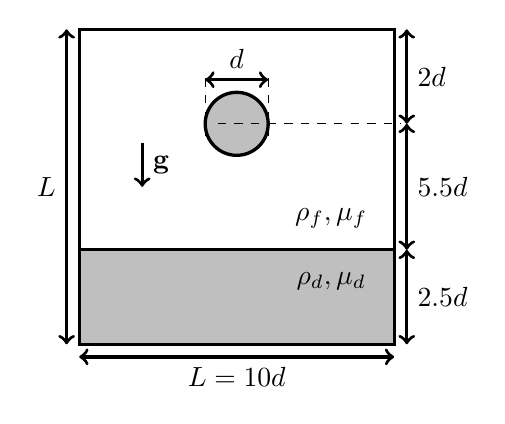
\begin{tikzpicture}[very thick,scale = 0.8]
        \draw (0,0) rectangle (5,5);
        \draw[fill=gray!50] (0,0) rectangle (5,1.5);
        \draw[fill=gray!50] (2.5,3.5) circle (0.5);
        \draw[<->](0,-0.2) --++ (5,0)node[midway,below]{$L  = 10 d$};
        \draw[<->](-0.2,0) --++ (0,5)node[midway,left]{$L$};
        \draw[<->](5.2,0) --++ (0,1.5)node[midway,right]{$2.5 d$};
        \draw[<->](5.2,1.5) --++ (0,2)node[midway,right]{$5.5 d$};
        \draw[<->](5.2,3.5) --++ (0,1.5)node[midway,right]{$ 2d$};
        \draw[dashed,thin](2.2,3.5) --++ (2.9,0);
        \draw[dashed,thin](2.2,3.5) --++ (2.9,0);
        \draw[->](1,3.2) --++ (0,-0.7)node[midway,right]{$\textbf{g}$};
        \draw[<->](2,4.2) --++ (1,0)node[midway,above]{$d$};
        \draw[thin,dashed](2,3.3) --++ (0,1);
        \draw[thin,dashed](3,3.3) --++ (0,1);
        \node (a) at (4,2){$\rho_f, \mu_f$};
        \node (a) at (4,1){$\rho_d, \mu_d$};
    \end{tikzpicture}
    \includegraphics[height = 0.3\textwidth]{image/VALIDATION2.0/Longmire/IMG/image-079.png}
    \caption{(left) Scheme of the computational set up at the initial time. 
    (right) Snapshot of the computational domain after the collision time, with the interfaces represented in gray.
    The background color represent the velocity field magnitude, which is undisturbed, indicating a large enough domain. }
    \label{fig:schemeLong}
\end{figure}
\begin{figure}[h!]
    \centering
    \includegraphics[height = 0.3\textwidth]{image/VALIDATION2.0/Longmire/Re.pdf}
    \includegraphics[height = 0.3\textwidth]{image/VALIDATION2.0/Longmire/Dist.pdf}
    \caption{(left) Time evolution of the Reynolds number based on the droplet velocity, $Re(t) = \rho_fU d /\mu_f$ in term of the dimensionless time, (+) numerical results of  \citet{balcazar2015multiple} (right)  position of the interfaces, ($\bullet$) top droplets surface, ($+$) bot droplet surface, (x) pool surface. (Symbols) experimental result of \citet{mohamed2003drop} (solid line) present numerical simulations with $d/\Delta = 30$. }
    \label{fig:resultslong}
\end{figure}
\ref{fig:resultslong} represent the comparison between our results against the experiment of \citet{mohamed2003drop} (right) and the numerical simulation of \citet{balcazar2015multiple} (left). 
The time dependent Reynolds number as well as the interfaces positions are shown to match exactly both, the numerical and experiential results of \citet{balcazar2015multiple} and \citet{mohamed2003drop}, respectively. 
From the very good agreement obtained with the numerical and experimental results we conclude that the kinematic is preserved during the contact time for a mesh definition of $d/\Delta = 30$. 

\subsection*{Mesh independence and statistical convergence for random array of drops}

Even through aforementioned studies carried validation of the \texttt{Basilisk} code for rising droplets or bubbles, almost all of them considered isolated droplets or bubbles as the only validation case. 
As far as the author's knowledge, to this date no published study presented a mesh independence study for random array of droplets nor bubbles of this scale. 
Nevertheless, as particles interaction and higher \textit{Galileo} numbers may be more challenging to model, it is primordial to investigate the mesh independence of the exact same DNS that are carried in this work. 
In this objective we performed DNS of random array of $N_b=125$ droplets, with the following parameters,
\begin{align*}
    \lambda = 10,
    && \zeta = 1.11,
    && Bo = 1,
    && Ga = 100,
    && \phi = 0.1,
    && N_b =125,
\end{align*}
and the mesh definition is, $d/\Delta = 7.37, 14.74, 29.9 58.97$. 
We expect that the most challenging DNS simulated in this work is for the case, $\lambda = 10$ and $Ga = 100$, since it is in this range of parameters that we induce the most vorticity, which ultimately require good mesh definition. 
Additionally, in opposition to the ordered array case, this case includes droplets interaction, which ultimately induce more numerical complexities to tackles. 
Based on this remark we can assume that if this case is mesh independent, then all cases from \ref{tab:simulations} must be since this is the most challenging scenario.   

Let's first verify the independence of the drift velocity on the mesh definition. 
\begin{figure}[h!]
    \centering
    \includegraphics[height = 0.3\textwidth]{image/HOMOGENEOUS_NEW/VAL/Re.pdf}
    \caption{
        Time evolution of the Reynolds number based on the instantaneous volume averaged drift velocity, $Re(t) = \rho_fU d /\mu_f$, with $U(t) = |\textbf{u}_p - \textbf{u}_f|$ with $\phi = 0.1256$, $\zeta =\mu_r =10$ and $Ga = 29.9$ for different mesh definition.
        $\textbf{u}_p$ and $\textbf{u}_f$ are the particle and fluid phase volume averaged velocity at time $t$.
        In the legend we display the value of the mesh definition and of the ensemble averaged Reynolds number. 
    }
    \label{fig:Re}
\end{figure}
In \ref{fig:Re} we display the instantaneous volume averaged drift velocity in terms of time, for four mesh definition. 
The results are not as independent of the mesh definition as the order array validation presented above. 
Indeed, we observe a difference of the rising Reynolds number of about $5\%$ between the $d/\Delta = 29.49$ and $d/\Delta = 58.97$ cases which is notable.
We recall that this $5\%$ error will eventually be lower for all other cases. 
The good agreement between the case  $d/\Delta = 14.74$ and $d/\Delta = 29.49$ is partially fortuitous.

Now let's study the mesh influence on the statistics. 
It is clear from \ref{fig:apstat} (left) that both mesh definition produce nearly the same radial distribution, no notable difference is identified. 
In \ref{fig:ap_age} (middle) we can observe the age distribution for both mesh definition. 
It is clear that refining the mesh induce a difference in the age distribution. 
As, a matter of fact it has a small impact on the mean age, $\tau_p = 6.96$ for the lower definition, and $\tau_p = 6.14$ for the finest grid.
This makes a $10\%$ error, but as mentioned above this is probably the highest error that we could encounter among all cases. 
\begin{figure}
    \centering
    \includegraphics[height = 0.24\textwidth]{image/HOMOGENEOUS_NEW/VAL/Pr.pdf}
    \includegraphics[height = 0.24\textwidth]{image/HOMOGENEOUS_NEW/VAL/Pa.pdf}
    \includegraphics[height = 0.24\textwidth]{image/HOMOGENEOUS_NEW/VAL/w.pdf}
    \caption{
        Statistical averaged functions for two mesh definition. 
        (left) Radial normalized probability density function  $P_r(\textbf{x},|\textbf{r}|,t)/P_\text{th}$, in terms of the dimensionless radial position. 
        (middle) Probability density function of the age distribution $P_a(\textbf{x},t,a)$. 
        (right) Nearest averaged dimensionless approach velocity for both mesh definition, in terms of the dimensionless age. 
    }
    \label{fig:apstat}
\end{figure}
Even through an error is identified on the mean age of interaction we still notice that both nearest averaged dimensionless approach velocity on \ref{fig:apstat} (right) match perfectly. 
\begin{figure}[h!]
    \centering
    \includegraphics[height = 0.3\textwidth]{image/HOMOGENEOUS_NEW/VAL/U_rel_ndc_25.pdf}
    \includegraphics[height = 0.3\textwidth]{image/HOMOGENEOUS_NEW/VAL/U_rel_ndc_35.pdf}
    \caption{Quiver plots of the relative averaged velocity field $\textbf{w}^\text{r}(\textbf{x},\textbf{r},t)$ colored by the averaged dimensionless age $a^r(\textbf{x},\textbf{r},t)$, for $\phi = 0.05$ and $Ga = 100$. 
    (left) Low mesh definition.
    (right) High mesh definition. 
    }
    \label{fig:velap}
\end{figure}
Regarding, the 2D fields  $\textbf{w}^\text{r}(\textbf{x},\textbf{r},t)$ we can see that no notable difference can be identified, if it is not the slight difference in the value of the age scale. 


Overall, the one dimensional and two-dimensional conditioned statistics are almost independent of the mesh definition. 
By obtaining the same statistics with two independent DNS makes us confident on the fact that our numerical samples is large enough.
Indeed, if the samples were not sufficient we would have obtained two different distribution functions, thus we can be sure that the statistics have well converged. 
The slight difference in rising velocity and age distribution found for these Reynolds number must be acknowledged.
As mentioned at the beginning, this case is in fact very challenging as the volume fraction of droplets is consequent which induce numerous inertial interactions. 
Nevertheless, we can be sure that our final results is accurate at most with a $5\%$ error for this case, and probably less for the others cases. 
Overall, we have great confidence in the statistical and physical representativity of our DNS results. 

The \texttt{Basilisk} code has been validated numerous time in previous numerical studies. 
Especially, we can cite the recent studies of \citet{innocenti2020direct} and \citet{hidman2023assessing} which both performed DNS of rising suspension of bubbles. 
Nevertheless, in this work we investigate specific statistical distribution,
and we make use of a multi-VoF method to avoid droplets coalescence, therefore a meticulous validation of the DNS is in order. 


\subsection*{Mesh independence and statistical convergence for random array of drops}

Even through aforementioned studies carried validation of the \texttt{Basilisk} code for rising droplets or bubbles, almost all of them considered isolated droplets or bubbles as the only validation case. 
As far as the author's knowledge, to this date no published study presented a mesh independence study for random array of droplets nor bubbles of this scale. 
Nevertheless, as particles interaction and higher \textit{Galileo} numbers may be more challenging to model, it is primordial to investigate the mesh independence of the exact same DNS that are carried in this work. 
In this objective we performed DNS of random array of $N_b=125$ droplets, with the following parameters,
\begin{align*}
    \lambda = 10,
    && \zeta = 1.11,
    && Bo = 1,
    && Ga = 100,
    && \phi = 0.1,
    && N_b =125,
\end{align*}
and the mesh definition is, $d/\Delta = 7.37, 14.74, 29.9 58.97$. 
We expect that the most challenging DNS simulated in this work is for the case, $\lambda = 10$ and $Ga = 100$, since it is in this range of parameters that we induce the most vorticity, which ultimately require good mesh definition. 
Additionally, in opposition to the ordered array case, this case includes droplets interaction, which ultimately induce more numerical complexities to tackles. 
Based on this remark we can assume that if this case is mesh independent, then all cases from \ref{tab:simulations} must be since this is the most challenging scenario.   

Now let's study the mesh influence on the statistics. 
It is clear from \ref{fig:apstat} (left) that both mesh definition produce nearly the same radial distribution, no notable difference is identified. 
In \ref{fig:apstat} (middle) we can observe the age distribution for both mesh definition. 
It is clear that refining the mesh induce a difference in the age distribution. 
As, a matter of fact it has a small impact on the mean age, $\tau_p = 6.96$ for the lower definition, and $\tau_p = 6.14$ for the finest grid.
This makes a $10\%$ error, but as mentioned above this is probably the highest error that we could encounter among all cases. 
\begin{figure}
    \centering
    \includegraphics[height = 0.24\textwidth]{image/HOMOGENEOUS_NEW/VAL/Pr.pdf}
    \includegraphics[height = 0.24\textwidth]{image/HOMOGENEOUS_NEW/VAL/Pa.pdf}
    \includegraphics[height = 0.24\textwidth]{image/HOMOGENEOUS_NEW/VAL/w.pdf}
    \caption{
        Statistical averaged functions for two mesh definition. 
        (left) Radial normalized probability density function  $P_r(\textbf{x},|\textbf{r}|,t)/P_\text{th}$, in terms of the dimensionless radial position. 
        (middle) Probability density function of the age distribution $P_a(\textbf{x},t,a)$. 
        (right) Nearest averaged dimensionless approach velocity for both mesh definition, in terms of the dimensionless age. 
    }
    \label{fig:apstat}
\end{figure}
Even through an error is identified on the mean duration of interaction we still note that both nearest averaged dimensionless approach velocity on \ref{fig:apstat} (right) match perfectly. 
\begin{figure}[h!]
    \centering
    \includegraphics[height = 0.3\textwidth]{image/HOMOGENEOUS_NEW/VAL/U_rel_ndc_25.pdf}
    \includegraphics[height = 0.3\textwidth]{image/HOMOGENEOUS_NEW/VAL/U_rel_ndc_35.pdf}
    \caption{Quiver plots of the relative averaged velocity field $\textbf{w}^\text{r}(\textbf{x},\textbf{r},t)$ colored by the averaged dimensionless age $a^r(\textbf{x},\textbf{r},t)$, for $\phi = 0.05$ and $Ga = 100$. 
    (left) Low mesh definition.
    (right) High mesh definition. 
    }
    \label{fig:velap}
\end{figure}
Regarding, the 2D fields  $\textbf{w}^\text{r}(\textbf{x},\textbf{r},t)$ we can see that no notable difference can be identified, if it is not the slight difference in the value of the age scale. 


Overall, the one dimensional and two-dimensional conditioned statistics are almost independent of the mesh definition. 
By obtaining the same statistics with two independent DNS makes us confident on the fact that our numerical samples is large enough.
Indeed, if the samples were not sufficient we would have obtained two different distribution functions, thus we can be sure that the statistics have well converged. 
The slight difference in rising velocity (see \citet[Appendix A]{fintzi2024buoyancy}) and age distribution found for these Reynolds number must be acknowledged.
As mentioned at the beginning, this case is in fact very challenging as the volume fraction of droplets is consequent which induce numerous inertial interactions. 
Nevertheless, we can be sure that our final results is accurate at most with a $5\%$ error for this case, and probably less for the others cases. 
These, error testify for the very challenging  aspect of these simulations. 
Overall, we have great confidence in the statistical and physical representativity of our DNS results. 

\section{Additional information}
\label{ap:age} 

% \begin{table}[h!]
%     \caption{Performance of the different functions used in a tri-periodic simulations. In this case we set $N_b = 125$, $Ga = 25$, $\phi = 0.1$ $\lambda = 1$. }
%     \label{tab:performance}
%     \begin{tabular}{c|c|c|c|l}
%     calls  &  total  &   self &  total  & function\\\hline
%     11393554 &  5123.85  & 5123.85 &    27.5\% (25.1\% - 30.4\%) &  mpi\_boundary\_level():grid/multigrid-mpi.h:83\\
%     2723 &  2210.91 &  2207.58  &   11.8\% ( 6.0\% - 12.5\%)&   dump():output.h:1160\\
%    54442 &  3116.87 &  2012.52  &   10.8\% ( 9.6\% - 11.8\%)&   project():poisson.h:501\\
%  3449898 &  1344.44 &  1344.44  &    7.2\% ( 5.0\% - 12.0\%)&   mpi\_all\_reduce0():common.h:683\\
%   113949 &  2140.47 &  1314.60  &    7.0\% ( 6.5\% -  7.5\%)&   heights():heights.h:281\\
%    27221 &  2694.78 &  1197.03  &    6.4\% ( 5.8\% -  7.0\%)&   vof\_0():vof.h:365\\
%    27221 &  1974.21 &  1191.03  &    6.4\% ( 5.9\% -  6.9\%)&   viscosity():viscosity.h:173\\
%    27221 &  2441.96 &  924.93   &   5.0\% ( 4.4\% -  5.4\%) &  advection\_term():navier-stokes/centered.h:323\\
%    27221 &  1853.70 &  733.94   &   3.9\% ( 3.9\% -  4.0\%) &  no\_coalescence():no-coalescence.h:419\\
%     2723 &  3006.33 &  571.93   &   3.1\% ( 2.4\% -  3.4\%) &  track\_bub():RS.c:124\\
%   341847 &  564.43  & 344.91    &  1.8\% ( 1.6\% -  2.2\%)  & reconstruction():fractions.h:476\\
%   113949 &  2988.98 &  317.86   &   1.7\% ( 1.4\% -  2.2\%) &  curvature():curvature.h:621\\
%    78825 &  1158.49 &  294.73   &   1.6\% ( 1.3\% -  1.7\%) &  tag():tag.h:268\\
%    27221 &  336.74  & 203.09    &  1.1\% ( 1.0\% -  1.2\%)  & acceleration\_0():iforce.h:133\\
%    27221 &  2246.89 &  180.53   &   1.0\% ( 0.8\% -  1.1\%) &  projection():navier-stokes/centered.h:430\\
%    27221 &  2085.36 &  111.14   &   0.6\% ( 0.5\% -  0.7\%) &  viscous\_term():navier-stokes/centered.h:362\\
%    27221 &  137.78  & 108.82    &  0.6\% ( 0.5\% -  0.7\%)  & acceleration\_2():RS.c:166\\
%    27222 &  108.68  & 108.64    &  0.6\% ( 0.4\% -  0.6\%)  & properties\_0():two-phase-generic.h:101\\
%    27221 &  174.57  & 102.50    &  0.5\% ( 0.5\% -  0.6\%)  & acceleration():navier-stokes/centered.h:386\\
%    81548 &   83.75  &  83.71    &  0.4\% ( 0.4\% -  0.7\%)  & z\_indexing():grid/multigrid-mpi.h:145\\
%      118 &   59.37  &  59.37    &  0.3\% ( 0.2\% -  0.7\%)  & compose\_image():view.h:409\\
%    27221 &   66.24  &  34.89    &  0.2\% ( 0.2\% -  0.2\%)  & tracer\_advection\_1():no-coalescence.h:446\\
%       59 &  130.73  &  28.79    &  0.2\% ( 0.1\% -  0.2\%)  & movies():RS.c:244\\
%    27222 &  360.96  &  24.44    &  0.1\% ( 0.1\% -  0.2\%)  & stability\_1():tension.h:64\\
%    27222 &   25.28  &  20.61    &  0.1\% ( 0.1\% -  0.1\%)  & stability():navier-stokes/centered.h:226\\
% 44143779 &  3190.44 &    5.87   &   0.0\% ( 0.0\% -  0.0\%) &  boundary\_internal():grid/cartesian-common.h:45\\
% 42200829 &   27.27  &   3.67    &  0.0\% ( 0.0\% -  0.0\%)  & interpolate():grid/cartesian-common.h:815\\
%      550 &    2.34  &   2.34    &  0.0\% ( 0.0\% -  0.0\%)  & draw\_vof():draw.h:1052\\
%    67429 &   37.19  &   1.13    &  0.0\% ( 0.0\% -  0.0\%)  & reduce\_bubbles():no-coalescence.h:158\\
% \end{tabular}
% \end{table}

\begin{table}  
\begin{tabular}{c|c|c|c|l}
  calls  &  total  &   self  & \% total  & function \\ \hline
  10636901 &  4861.39 &  4861.39  &   31.8\% (28.4\% - 36.7\%) &   mpi\_boundary\_level():grid/multigrid-mpi.h:83\\
     53604 &  3097.64 &  1988.97  &   13.0\% (10.8\% - 14.7\%) &   project():poisson.h:501\\
     26802 &  2022.99 &  1236.57  &    8.1\% ( 7.3\% -  8.8\%) &   viscosity():viscosity.h:173\\
    107208 &  1984.59 &  1223.33  &    8.0\% ( 6.9\% -  8.9\%) &   heights():heights.h:281\\
     26802 &  2499.81 &  1099.66  &    7.2\% ( 6.1\% -  7.9\%) &   vof\_0():vof.h:365\\
   3155070 &  983.66  & 983.66    &  6.4\% ( 3.9\% -  9.1\%)   & mpi\_all\_reduce0():common.h:683\\
     26802 &  2372.23 &  896.09   &   5.9\% ( 5.1\% -  6.5\%)  &  advection\_term():navier-stokes/centered.h:323\\
     26802 &  1583.59 &  645.89   &   4.2\% ( 4.1\% -  4.3\%)  &  no\_coalescence():./no-coalescence.h:419\\
      2681 &  584.39  & 372.15    &  2.4\% ( 2.4\% -  2.5\%)   & track\_bub():RS.c:124\\
    321624 &  546.74  & 340.36    &  2.2\% ( 1.8\% -  2.6\%)   & reconstruction():fractions.h:476\\
    107208 &  2777.30 &  303.23   &   2.0\% ( 1.6\% -  2.4\%)  &  curvature():curvature.h:621\\
     69275 &  992.44  & 254.14    &  1.7\% ( 1.4\% -  1.8\%)   & tag():tag.h:268\\
     26802 &  328.67  & 202.85    &  1.3\% ( 1.1\% -  1.5\%)   & acceleration\_0():iforce.h:133\\
     26802 &  2257.27 &  178.19   &   1.2\% ( 0.8\% -  1.3\%)  &  projection():navier-stokes/centered.h:430\\
     26802 &  2142.30 &  119.30   &   0.8\% ( 0.5\% -  0.9\%)  &  viscous\_term():navier-stokes/centered.h:362\\
     26802 &  145.95  & 116.09    &  0.8\% ( 0.5\% -  0.9\%)   & acceleration\_2():RS.c:166\\
     26803 &  111.60  & 111.57    &  0.7\% ( 0.5\% -  0.8\%)   & properties\_0():two-phase-generic.h:101\\
     26802 &  172.09  & 100.18    &  0.7\% ( 0.5\% -  0.8\%)   & acceleration():navier-stokes/centered.h:386\\
     69275 &   68.91  &  68.88    &  0.5\% ( 0.4\% -  0.5\%)   & z\_indexing():grid/multigrid-mpi.h:145\\
       118 &   59.59  &  59.59    &  0.4\% ( 0.2\% -  0.8\%)   & compose\_image():view.h:409\\
     26802 &   64.69  &  34.48    &  0.2\% ( 0.2\% -  0.3\%)   & tracer\_advection\_1():./no-coalescence.h:446\\
        59 &  129.57  &  28.81    &  0.2\% ( 0.1\% -  0.2\%)   & movies():RS.c:244\\
     26803 &   92.48  &  27.24    &  0.2\% ( 0.1\% -  0.2\%)   & stability\_1():tension.h:64\\
     26803 &   24.42  &  21.33    &  0.1\% ( 0.1\% -  0.1\%)   & stability():navier-stokes/centered.h:226\\
  43894361 &  3001.24 &    5.50   &   0.0\% ( 0.0\% -  0.0\%)  &  boundary\_internal():grid/cartesian-common.h:450\\
  42061052 &   25.50  &   3.61    &  0.0\% ( 0.0\% -  0.0\%)   & interpolate():grid/cartesian-common.h:815\\
       472 &    2.31  &   2.31    &  0.0\% ( 0.0\% -  0.0\%)   & draw\_vof():draw.h:1052\\
     58554 &   25.92  &   0.87    &  0.0\% ( 0.0\% -  0.0\%)   & reduce\_bubbles():./no-coalescence.h:158\\
         1 &  15287.89&     0.73  &    0.0\% ( 0.0\% -  0.0\%) &   run():run.h:37\\
         1 &    0.28  &   0.28    &  0.0\% ( 0.0\% -  0.0\%)   & init\_0():RS.c:149\\
     26802 &  2777.57 &    0.27   &   0.0\% ( 0.0\% -  0.0\%)  &  acceleration\_1():tension.h:94\\
       236 &   38.81  &   0.21    &  0.0\% ( 0.0\% -  0.0\%)   & squares():draw.h:1375\\
    %    118 &   59.64  &   0.05    &  0.0\% ( 0.0\% -  0.1\%)   & save():view.h:529\\
    %  63404 &    0.06  &   0.03    &  0.0\% ( 0.0\% -  0.0\%)   & interpolate():grid/cartesian-common.h:816\\
    %      1 &    0.02  &   0.02    &  0.0\% ( 0.0\% -  0.0\%)   & defaults\_3():iforce.h:38\\
    %      1 &    0.01  &   0.01    &  0.0\% ( 0.0\% -  0.0\%)   & defaults\_2():two-phase-generic.h:26\\
    %  26802 &  1583.60 &    0.01   &   0.0\% ( 0.0\% -  0.0\%)  &  vof\_1():./no-coalescence.h:430\\
    %  26802 &    0.01  &   0.01    &  0.0\% ( 0.0\% -  0.0\%)   & set\_dtmax():navier-stokes/centered.h:222\\
    %  26803 &    0.00  &   0.00    &  0.0\% ( 0.0\% -  0.0\%)   & stability\_0():vof.h:143\\
    %      1 &    0.25  &   0.00    &  0.0\% ( 0.0\% -  0.0\%)   & init():navier-stokes/centered.h:213\\
    %      1 &    0.00  &   0.00    &  0.0\% ( 0.0\% -  0.0\%)   & defaults\_0():navier-stokes/centered.h:181\\
    %      1 &    0.00  &   0.00    &  0.0\% ( 0.0\% -  0.0\%)   & restore():output.h:1169\\
    %      1 &    0.00  &   0.00    &  0.0\% ( 0.0\% -  0.0\%)   & cleanup():run.h:52\\
    %      1 &    0.00  &   0.00    &  0.0\% ( 0.0\% -  0.0\%)   & defaults():run.h:44\\
    %      1 &    0.00  &   0.00    &  0.0\% ( 0.0\% -  0.0\%)   & defaults\_4():./no-coalescence.h:483\\
    %      1 &    0.00  &   0.00    &  0.0\% ( 0.0\% -  0.0\%)   & defaults\_1():vof.h:134\\
    %      1 &    0.00  &   0.00    &  0.0\% ( 0.0\% -  0.0\%)   & cleanup\_0():./no-coalescence.h:458\\
    %      1 &    0.00  &   0.00    &  0.0\% ( 0.0\% -  0.0\%)   & default\_display():navier-stokes/centered.h:188\\
    %      1 &    0.00  &   0.00    &  0.0\% ( 0.0\% -  0.0\%)   & stop():RS.c:272\\
\end{tabular}
\caption{Output of the basilisk compiler tool that measures algorithm performance all along the simulation.}
\end{table}



In this appendix we provide additional graph to support the argumentation made in the main text. 
Additional Radial distribution functions, 
\begin{figure}[h!]
    \centering
    % \includegraphics[height=0.3\textwidth]{image/HOMOGENEOUS_NEW/Dist/Pr_l_1_Ga_100.pdf}
    % \includegraphics[height=0.3\textwidth]{image/HOMOGENEOUS_NEW/Dist/Pr_l_10_Ga_100.pdf}
    \includegraphics[height=0.3\textwidth]{image/HOMOGENEOUS_NEW/Dist/Pr_l_1_Ga_10.pdf}
    \includegraphics[height=0.3\textwidth]{image/HOMOGENEOUS_NEW/Dist/Pr_l_10_Ga_10.pdf}
    \caption{Radial probability density function $P_\text{nst}^n(\textbf{x},t,r)$ divided by the theoretical distribution $P_\text{nst}^{th}$ \ref{eq:Pnst_dilute}, in terms of the dimensionless distance $(r-d)/d_p$ where, $d_p = n_p^{-1/3}$, for  $Ga = 10$.
    (left)  $\lambda = 1$.
    (right) $\lambda = 10$.
    ($\pmb\bigcirc$) $\phi = 0.01$; ($\pmb\triangle$) $ \phi = 0.05$; ($\pmb\square$) $\phi = 0.1$ ($\pmb\lozenge$) $\phi = 0.2$.
    (dashed lines) Theoretical prediction : $P_\text{nst}^n/P_\text{nst}^\text{th} = 1$. 
    For $r<d$ we arbitrarily set $P_\text{nst}^\text{th} = 1$ so that the distribution can be visualized.
    }
    \label{fig:Pr_low}
\end{figure}
The drift velocity used in \ref{fig:age_picture} is given \ref{fig:Reall}.
\begin{figure}[h!]
    \centering
    \includegraphics[height = 0.3\textwidth]{image/HOMOGENEOUS_NEW/CA/Re_l_1.pdf}
    \includegraphics[height = 0.3\textwidth]{image/HOMOGENEOUS_NEW/CA/Re_l_10.pdf}
    \caption{
        Averaged Reynolds number based on the averaged drift velocity, $Re = \rho_fU d /\mu_f$, with $U = |\textbf{u}_p - \textbf{u}_f|$.
        $\textbf{u}_p$ and $\textbf{u}_f$ are the particle and fluid phase volume and time averaged velocity.
    }
    \label{fig:Reall}
\end{figure}
We provide additional age distribution for low \textit{Galileo} number to support the argumentation in the body of the text. 
\begin{figure}[h!]
    \centering
    \includegraphics[height = 0.3\textwidth]{image/HOMOGENEOUS_NEW/Dist/Pa_l_1_Ga_10.pdf}
    \includegraphics[height = 0.3\textwidth]{image/HOMOGENEOUS_NEW/Dist/Pa_l_10_Ga_10.pdf}
    \caption{(left) Age distribution at $\lambda = 10$ and $Ga = 10$ for : (solid line) $\phi = 0.2$; (dash dotted line) $\phi = 0.1$; (dashed line) $\phi =0.05$; (dotted line) $\phi = 0.01$. 
    (right) Mean dimensionless age in terms of the volume fraction $\phi$ for : 
    ($\pmb\bigcirc$) $Ga=1$; ($\pmb\triangle$) $ Ga = 10$; ($\pmb\square$) $Ga = 50$ ($\pmb\lozenge$) $Ga =100$.
    The age and $\tau_a$ are made dimensionless with $U/d$ where $U$ is the drift-velocity between the dispersed and continuous phase.  }
    \label{fig:age_picture_low_ga}
\end{figure}


\addcontentsline{toc}{chapter}{Bibliography}
\bibliography{Bib/bib_bulles.bib}


\end{document}
